% Generated by Sphinx.
\def\sphinxdocclass{report}
\documentclass[letterpaper,10pt,english]{sphinxmanual}
\usepackage[utf8]{inputenc}
\DeclareUnicodeCharacter{00A0}{\nobreakspace}
\usepackage{cmap}
\usepackage[T1]{fontenc}
\usepackage{babel}
\usepackage{times}
\usepackage[Bjarne]{fncychap}
\usepackage{longtable}
\usepackage{sphinx}
\usepackage{multirow}

\usepackage{xeCJK}
\usepackage{indentfirst}
\setlength{\parindent}{2em}
\setCJKmainfont{WenQuanYi Zen Hei Sharp}
\setCJKmonofont[Scale=0.9]{WenQuanYi Zen Hei Mono}
\setCJKfamilyfont{song}{WenQuanYi Zen Hei}
\setCJKfamilyfont{sf}{WenQuanYi Zen Hei}


\title{biopython\_cn Documentation}
\date{January 23, 2014}
\release{0.1}
\author{biopythoners}
\newcommand{\sphinxlogo}{}
\renewcommand{\releasename}{Release}
\makeindex

\makeatletter
\def\PYG@reset{\let\PYG@it=\relax \let\PYG@bf=\relax%
    \let\PYG@ul=\relax \let\PYG@tc=\relax%
    \let\PYG@bc=\relax \let\PYG@ff=\relax}
\def\PYG@tok#1{\csname PYG@tok@#1\endcsname}
\def\PYG@toks#1+{\ifx\relax#1\empty\else%
    \PYG@tok{#1}\expandafter\PYG@toks\fi}
\def\PYG@do#1{\PYG@bc{\PYG@tc{\PYG@ul{%
    \PYG@it{\PYG@bf{\PYG@ff{#1}}}}}}}
\def\PYG#1#2{\PYG@reset\PYG@toks#1+\relax+\PYG@do{#2}}

\expandafter\def\csname PYG@tok@gd\endcsname{\def\PYG@tc##1{\textcolor[rgb]{0.63,0.00,0.00}{##1}}}
\expandafter\def\csname PYG@tok@gu\endcsname{\let\PYG@bf=\textbf\def\PYG@tc##1{\textcolor[rgb]{0.50,0.00,0.50}{##1}}}
\expandafter\def\csname PYG@tok@gt\endcsname{\def\PYG@tc##1{\textcolor[rgb]{0.00,0.27,0.87}{##1}}}
\expandafter\def\csname PYG@tok@gs\endcsname{\let\PYG@bf=\textbf}
\expandafter\def\csname PYG@tok@gr\endcsname{\def\PYG@tc##1{\textcolor[rgb]{1.00,0.00,0.00}{##1}}}
\expandafter\def\csname PYG@tok@cm\endcsname{\let\PYG@it=\textit\def\PYG@tc##1{\textcolor[rgb]{0.25,0.50,0.56}{##1}}}
\expandafter\def\csname PYG@tok@vg\endcsname{\def\PYG@tc##1{\textcolor[rgb]{0.73,0.38,0.84}{##1}}}
\expandafter\def\csname PYG@tok@m\endcsname{\def\PYG@tc##1{\textcolor[rgb]{0.13,0.50,0.31}{##1}}}
\expandafter\def\csname PYG@tok@mh\endcsname{\def\PYG@tc##1{\textcolor[rgb]{0.13,0.50,0.31}{##1}}}
\expandafter\def\csname PYG@tok@cs\endcsname{\def\PYG@tc##1{\textcolor[rgb]{0.25,0.50,0.56}{##1}}\def\PYG@bc##1{\setlength{\fboxsep}{0pt}\colorbox[rgb]{1.00,0.94,0.94}{\strut ##1}}}
\expandafter\def\csname PYG@tok@ge\endcsname{\let\PYG@it=\textit}
\expandafter\def\csname PYG@tok@vc\endcsname{\def\PYG@tc##1{\textcolor[rgb]{0.73,0.38,0.84}{##1}}}
\expandafter\def\csname PYG@tok@il\endcsname{\def\PYG@tc##1{\textcolor[rgb]{0.13,0.50,0.31}{##1}}}
\expandafter\def\csname PYG@tok@go\endcsname{\def\PYG@tc##1{\textcolor[rgb]{0.20,0.20,0.20}{##1}}}
\expandafter\def\csname PYG@tok@cp\endcsname{\def\PYG@tc##1{\textcolor[rgb]{0.00,0.44,0.13}{##1}}}
\expandafter\def\csname PYG@tok@gi\endcsname{\def\PYG@tc##1{\textcolor[rgb]{0.00,0.63,0.00}{##1}}}
\expandafter\def\csname PYG@tok@gh\endcsname{\let\PYG@bf=\textbf\def\PYG@tc##1{\textcolor[rgb]{0.00,0.00,0.50}{##1}}}
\expandafter\def\csname PYG@tok@ni\endcsname{\let\PYG@bf=\textbf\def\PYG@tc##1{\textcolor[rgb]{0.84,0.33,0.22}{##1}}}
\expandafter\def\csname PYG@tok@nl\endcsname{\let\PYG@bf=\textbf\def\PYG@tc##1{\textcolor[rgb]{0.00,0.13,0.44}{##1}}}
\expandafter\def\csname PYG@tok@nn\endcsname{\let\PYG@bf=\textbf\def\PYG@tc##1{\textcolor[rgb]{0.05,0.52,0.71}{##1}}}
\expandafter\def\csname PYG@tok@no\endcsname{\def\PYG@tc##1{\textcolor[rgb]{0.38,0.68,0.84}{##1}}}
\expandafter\def\csname PYG@tok@na\endcsname{\def\PYG@tc##1{\textcolor[rgb]{0.25,0.44,0.63}{##1}}}
\expandafter\def\csname PYG@tok@nb\endcsname{\def\PYG@tc##1{\textcolor[rgb]{0.00,0.44,0.13}{##1}}}
\expandafter\def\csname PYG@tok@nc\endcsname{\let\PYG@bf=\textbf\def\PYG@tc##1{\textcolor[rgb]{0.05,0.52,0.71}{##1}}}
\expandafter\def\csname PYG@tok@nd\endcsname{\let\PYG@bf=\textbf\def\PYG@tc##1{\textcolor[rgb]{0.33,0.33,0.33}{##1}}}
\expandafter\def\csname PYG@tok@ne\endcsname{\def\PYG@tc##1{\textcolor[rgb]{0.00,0.44,0.13}{##1}}}
\expandafter\def\csname PYG@tok@nf\endcsname{\def\PYG@tc##1{\textcolor[rgb]{0.02,0.16,0.49}{##1}}}
\expandafter\def\csname PYG@tok@si\endcsname{\let\PYG@it=\textit\def\PYG@tc##1{\textcolor[rgb]{0.44,0.63,0.82}{##1}}}
\expandafter\def\csname PYG@tok@s2\endcsname{\def\PYG@tc##1{\textcolor[rgb]{0.25,0.44,0.63}{##1}}}
\expandafter\def\csname PYG@tok@vi\endcsname{\def\PYG@tc##1{\textcolor[rgb]{0.73,0.38,0.84}{##1}}}
\expandafter\def\csname PYG@tok@nt\endcsname{\let\PYG@bf=\textbf\def\PYG@tc##1{\textcolor[rgb]{0.02,0.16,0.45}{##1}}}
\expandafter\def\csname PYG@tok@nv\endcsname{\def\PYG@tc##1{\textcolor[rgb]{0.73,0.38,0.84}{##1}}}
\expandafter\def\csname PYG@tok@s1\endcsname{\def\PYG@tc##1{\textcolor[rgb]{0.25,0.44,0.63}{##1}}}
\expandafter\def\csname PYG@tok@gp\endcsname{\let\PYG@bf=\textbf\def\PYG@tc##1{\textcolor[rgb]{0.78,0.36,0.04}{##1}}}
\expandafter\def\csname PYG@tok@sh\endcsname{\def\PYG@tc##1{\textcolor[rgb]{0.25,0.44,0.63}{##1}}}
\expandafter\def\csname PYG@tok@ow\endcsname{\let\PYG@bf=\textbf\def\PYG@tc##1{\textcolor[rgb]{0.00,0.44,0.13}{##1}}}
\expandafter\def\csname PYG@tok@sx\endcsname{\def\PYG@tc##1{\textcolor[rgb]{0.78,0.36,0.04}{##1}}}
\expandafter\def\csname PYG@tok@bp\endcsname{\def\PYG@tc##1{\textcolor[rgb]{0.00,0.44,0.13}{##1}}}
\expandafter\def\csname PYG@tok@c1\endcsname{\let\PYG@it=\textit\def\PYG@tc##1{\textcolor[rgb]{0.25,0.50,0.56}{##1}}}
\expandafter\def\csname PYG@tok@kc\endcsname{\let\PYG@bf=\textbf\def\PYG@tc##1{\textcolor[rgb]{0.00,0.44,0.13}{##1}}}
\expandafter\def\csname PYG@tok@c\endcsname{\let\PYG@it=\textit\def\PYG@tc##1{\textcolor[rgb]{0.25,0.50,0.56}{##1}}}
\expandafter\def\csname PYG@tok@mf\endcsname{\def\PYG@tc##1{\textcolor[rgb]{0.13,0.50,0.31}{##1}}}
\expandafter\def\csname PYG@tok@err\endcsname{\def\PYG@bc##1{\setlength{\fboxsep}{0pt}\fcolorbox[rgb]{1.00,0.00,0.00}{1,1,1}{\strut ##1}}}
\expandafter\def\csname PYG@tok@kd\endcsname{\let\PYG@bf=\textbf\def\PYG@tc##1{\textcolor[rgb]{0.00,0.44,0.13}{##1}}}
\expandafter\def\csname PYG@tok@ss\endcsname{\def\PYG@tc##1{\textcolor[rgb]{0.32,0.47,0.09}{##1}}}
\expandafter\def\csname PYG@tok@sr\endcsname{\def\PYG@tc##1{\textcolor[rgb]{0.14,0.33,0.53}{##1}}}
\expandafter\def\csname PYG@tok@mo\endcsname{\def\PYG@tc##1{\textcolor[rgb]{0.13,0.50,0.31}{##1}}}
\expandafter\def\csname PYG@tok@mi\endcsname{\def\PYG@tc##1{\textcolor[rgb]{0.13,0.50,0.31}{##1}}}
\expandafter\def\csname PYG@tok@kn\endcsname{\let\PYG@bf=\textbf\def\PYG@tc##1{\textcolor[rgb]{0.00,0.44,0.13}{##1}}}
\expandafter\def\csname PYG@tok@o\endcsname{\def\PYG@tc##1{\textcolor[rgb]{0.40,0.40,0.40}{##1}}}
\expandafter\def\csname PYG@tok@kr\endcsname{\let\PYG@bf=\textbf\def\PYG@tc##1{\textcolor[rgb]{0.00,0.44,0.13}{##1}}}
\expandafter\def\csname PYG@tok@s\endcsname{\def\PYG@tc##1{\textcolor[rgb]{0.25,0.44,0.63}{##1}}}
\expandafter\def\csname PYG@tok@kp\endcsname{\def\PYG@tc##1{\textcolor[rgb]{0.00,0.44,0.13}{##1}}}
\expandafter\def\csname PYG@tok@w\endcsname{\def\PYG@tc##1{\textcolor[rgb]{0.73,0.73,0.73}{##1}}}
\expandafter\def\csname PYG@tok@kt\endcsname{\def\PYG@tc##1{\textcolor[rgb]{0.56,0.13,0.00}{##1}}}
\expandafter\def\csname PYG@tok@sc\endcsname{\def\PYG@tc##1{\textcolor[rgb]{0.25,0.44,0.63}{##1}}}
\expandafter\def\csname PYG@tok@sb\endcsname{\def\PYG@tc##1{\textcolor[rgb]{0.25,0.44,0.63}{##1}}}
\expandafter\def\csname PYG@tok@k\endcsname{\let\PYG@bf=\textbf\def\PYG@tc##1{\textcolor[rgb]{0.00,0.44,0.13}{##1}}}
\expandafter\def\csname PYG@tok@se\endcsname{\let\PYG@bf=\textbf\def\PYG@tc##1{\textcolor[rgb]{0.25,0.44,0.63}{##1}}}
\expandafter\def\csname PYG@tok@sd\endcsname{\let\PYG@it=\textit\def\PYG@tc##1{\textcolor[rgb]{0.25,0.44,0.63}{##1}}}

\def\PYGZbs{\char`\\}
\def\PYGZus{\char`\_}
\def\PYGZob{\char`\{}
\def\PYGZcb{\char`\}}
\def\PYGZca{\char`\^}
\def\PYGZam{\char`\&}
\def\PYGZlt{\char`\<}
\def\PYGZgt{\char`\>}
\def\PYGZsh{\char`\#}
\def\PYGZpc{\char`\%}
\def\PYGZdl{\char`\$}
\def\PYGZhy{\char`\-}
\def\PYGZsq{\char`\'}
\def\PYGZdq{\char`\"}
\def\PYGZti{\char`\~}
% for compatibility with earlier versions
\def\PYGZat{@}
\def\PYGZlb{[}
\def\PYGZrb{]}
\makeatother

\setcounter{secnumdepth}{0}

\begin{document}

\maketitle
\tableofcontents
\phantomsection\label{index::doc}


Contents:


\chapter{第1章 介绍}
\label{chr01:welcome-to-biopython-cn-s-documentation}\label{chr01::doc}\label{chr01:id1}

\section{1.1  什么是Biopython?}
\label{chr01:biopython}
Biopython工程是一个使用Python来开发计算分子生物学工具的国际团体。(\href{http://www.python.org}{http://www.python.org})
Python是一种面向对象的、解释型的、灵活的语言,在计算机科学中日益流行。Python易学,语法明晰,并且能很容易的使用以C,C++或
者FORTRAN编写的模块实现扩展。

Biopython官网(\href{http://www.biopython.org}{http://www.biopython.org})为使用和研究生物信息学的开发者提供了一个在线的
资源库,包括模块、脚本以及一些基于Python的软件的网站链接。一般来讲,Biopython致力于通过创造高质量的和可重复利用的模块及
类,从而使得Python在生物信息学中的应用变得更加容易。Biopython的特点包括解析各种生物信息学格式的文件(BLAST, Clustalw, FASTA,
Genbank...),访问在线的服务器(NCBI,Expasy...),常见和不那么常见程序的接口(Clustalw, DSSP,MSMS...),标准的序列类,各
种收集的模块,KD树数据结构等等,还有一些文档。

基本来说,我们喜欢使用Python来编程,并且希望通过创建高质量、可复用的模块和脚本来使得Python在生物信息学中的应用变得容易。


\section{1.2  在Biopython包中我能发现什么?}
\label{chr01:id2}
主要的Biopython发行版本有很多种功能,包括:
\begin{itemize}
\item {} 
将生物信息学文件解析为Python可用的数据结构,包含以下支持的格式:
\begin{itemize}
\item {} 
Blast输出结果 – standalone和在线Blast

\item {} 
Clustalw

\item {} 
FASTA

\item {} 
GenBank

\item {} 
PubMed和Medline

\item {} 
ExPASy文件, 如Enzyme和Prosite

\item {} 
SCOP, 包括‘dom’和‘lin’文件

\item {} 
UniGene

\item {} 
SwissProt

\end{itemize}

\item {} 
被支持格式的文件可以通过记录来重复或者通过字典界面来索引。

\item {} 
处理常见的生物信息学在线数据库的代码:
\begin{itemize}
\item {} 
NCBI – Blast, Entrez和PubMed服务

\item {} 
ExPASy – Swiss-Prot和Prosite条目, 包括Prosite搜索

\end{itemize}

\item {} 
常见生物信息学程序的接口,例如:
\begin{itemize}
\item {} 
NCBI的Standalone Blast

\item {} 
Clustalw比对程序

\item {} 
EMBOSS命令行工具

\end{itemize}

\item {} 
一个能处理序列、ID和序列特征的标准序列类。

\item {} 
对序列实现常规操作的工具,如翻译,转录和权重计算。

\item {} 
利用k最近邻接、Bayes或SVM对数据进行分类的代码。

\item {} 
处理比对的代码,包括创建和处理替换矩阵的标准方法。

\item {} 
分发并行任务到不同进程的代码。

\item {} 
实现序列的基本操作,翻译以及BLAST等功能的GUI程序。

\item {} 
使用这些模块的详细文档和帮助,包括此文件,在线的wiki文档,网站和邮件列表。

\item {} 
整合BioSQL,一个也被BioPerl和BioJava支持的数据库架构。

\end{itemize}

我们希望这些能给你足够的理由去下载并开始使用Biopython!


\section{1.3  安装Biopython}
\label{chr01:id3}
Biopython的所有安装信息在此文档中分开,以便于更容易保持更新。

简短的版本去我们的下载页面(\href{http://biopython.org/wiki/Download}{http://biopython.org/wiki/Download}),
下载并安装所列举的dependencies,然后下载并安装Biopython。Biopython能在多种平台上运行(Windows,Mac,各种版本的Linux和Unix)。
对于Windows我们提供预编译的一键式安装程序,而对Unix和其他操作系统,你必须按照附带的README文件从源开始安装。这通常
是很简单的,只要标准命令:
\DUspan{name}{}\DUspan{name}{}\DUspan{operator}{}\DUspan{name}{}\DUspan{name}{}\DUspan{name}{}\DUspan{name}{}\DUspan{operator}{}\DUspan{name}{}\DUspan{name}{}\DUspan{name}{}\DUspan{name}{}\DUspan{name}{}\DUspan{operator}{}\DUspan{name}{}\DUspan{name}{}
\begin{Verbatim}[commandchars=\\\{\}]
python setup.py build
python setup.py test
sudo python setup.py install
\end{Verbatim}

(事实上你可以跳过build和test,直接install。但最好是确保所有的东西看起来都没问题。)

我们的安装说明的详细版本包括了Python的安装,Biopython dependencies的安装以及Biopython本身的安装。可从PDF
(\href{http://biopython.org/DIST/docs/install/Installation.pdf}{http://biopython.org/DIST/docs/install/Installation.pdf})
和HTML格式获得。
(\href{http://biopython.org/DIST/docs/install/Installation.html}{http://biopython.org/DIST/docs/install/Installation.html})。


\section{1.4  常见问答(FAQ)}
\label{chr01:faq}\begin{enumerate}
\item {} 
\emph{在科学出版中我怎样引用Biopython?}

请引用我们的应用笔记 {[}{\hyperref[chr23:cock2009]{\emph{1}}}, Cock \emph{et al.} ,  2009{]} 作为主要的Biopython参考文献。另外,如果可以,请
引用以下任意出版物,特别是作为Biopython特定模块的参考文献的话。
(更多信息可在我们网站上获得):
\begin{itemize}
\item {} 
对于官方项目声明: {[}{\hyperref[chr23:chapman2000]{\emph{13}}},
Chapman and Chang, 2000{]};

\item {} 
对于 \code{Bio.PDB}: {[}{\hyperref[chr23:hamelryck2003a]{\emph{18}}}, Hamelryck and
Manderick, 2003{]};

\item {} 
对于 \code{Bio.Cluster}: {[}{\hyperref[chr23:dehoon2004]{\emph{14}}}, De Hoon \emph{et al.},
2004{]};

\item {} 
对于 \code{Bio.Graphics.GenomeDiagram}: {[}{\hyperref[chr23:pritchard2006]{\emph{2}}},
Pritchard \emph{et al.}, 2006{]};

\item {} 
对于 \code{Bio.Phylo} 和 \code{Bio.Phylo.PAML}: {[}{\hyperref[chr23:talevich2012]{\emph{9}}},
Talevich \emph{et al.}, 2012{]};

\item {} 
对于在Biopython,BioPerl,BioRuby,BioJava和EMBOSS支持的FASTQ格
式文件:{[}{\hyperref[chr23:cock2010]{\emph{7}}}, Cock \emph{et al.}, 2010{]}.

\end{itemize}

\item {} 
\emph{我该怎样以大写字母写“Biopython”?写成“BioPython”可以吗?}

正确的大写是“Biopython”而不是“BioPython”(虽然对于BioPerl,BioRuby
和BioJava是这样)。

\item {} 
\emph{我怎样查看自己安装的Biopython的版本?}

使用以下代码:
\DUspan{operator}{}\DUspan{keyword,namespace}{}\DUspan{name,namespace}{}\DUspan{operator}{}\DUspan{keyword}{}\DUspan{name}{}\DUspan{operator}{}\DUspan{name}{}\DUspan{operator}{}
\begin{Verbatim}[commandchars=\\\{\}]
\PYG{g+gp}{\PYGZgt{}\PYGZgt{}\PYGZgt{} }\PYG{k+kn}{import} \PYG{n+nn}{Bio}
\PYG{g+gp}{\PYGZgt{}\PYGZgt{}\PYGZgt{} }\PYG{k}{print} \PYG{n}{Bio}\PYG{o}{.}\PYG{n}{\PYGZus{}\PYGZus{}version\PYGZus{}\PYGZus{}}
\PYG{g+gp}{...}
\end{Verbatim}

如果 “\code{import Bio}” 这行报错,说明Biopython未被安装。如果第二行报错,
你的版本已经很过时了。如果版本号以“+”号结束,说明你用的并不是官方版本,而
是开发代码的快照。

\item {} 
\emph{此文档的最新版本在哪里?}

如果你下载的是一个Biopython源代码包,那么它将包含此文档HTML和PDF两种格式
的相应版本。此文档最新出版的版本可通过在线获得(每个版本的更新):
\begin{itemize}
\item {} 
\href{http://biopython.org/DIST/docs/tutorial/Tutorial.html}{http://biopython.org/DIST/docs/tutorial/Tutorial.html}

\item {} 
\href{http://biopython.org/DIST/docs/tutorial/Tutorial.pdf}{http://biopython.org/DIST/docs/tutorial/Tutorial.pdf}

\end{itemize}

如果你使用的是从我们库中获得的尚未发布的最新代码,你可以在这里找到还在开发中
的教程的拷贝:
\begin{itemize}
\item {} 
\href{http://biopython.org/DIST/docs/tutorial/Tutorial-dev.html}{http://biopython.org/DIST/docs/tutorial/Tutorial-dev.html}

\item {} 
\href{http://biopython.org/DIST/docs/tutorial/Tutorial-dev.pdf}{http://biopython.org/DIST/docs/tutorial/Tutorial-dev.pdf}

\end{itemize}

\item {} 
\emph{我需要哪一个“Numerical Python”?}

对于Biopython 1.48或更早的版本,你需要老的Numeric模块。对于Biopython 1.49
及更高的版本,你需要更新的NumPy来代替。Numeric和NumPy都可以在同一台机器上安
装。也可以访问: \href{http://numpy.scipy.org/}{http://numpy.scipy.org/}

\item {} 
\emph{为什么} \code{Seq} \emph{对象缺少了这篇教程里的(反向)transcription和translation方法?}

你需要Biopython 1.49或更新的版本。或者,使用以下 {\hyperref[chr03:sec-seq-module-functions]{\emph{3.14}}} 部分中的 \code{Bio.Seq} 模块
功能。

\item {} 
\emph{为什么} \code{Seq} \emph{对象缺少了这篇教程中的upper和lower方法?}

你需要Biopython 1.53或更新版本。或者,使用 \code{str(my\_seq).upper()} 来获得
大写字符串。如果你需要一个Seq对象,试试 \code{Seq(str(my\_seq).upper())} ,但是
要小心重用相同的字母。

\item {} 
\emph{为什么} \code{Seq} \emph{对象的translation方法不支持本教程中描述的} \code{cds} \emph{选项?}

你需要Biopython 1.51或更新版本。

\item {} 
\emph{为什么} \code{Bio.SeqIO} \emph{不能正常工作?它导入正常但是没有解析函数等。}

你需要Biopython 1.43或更新版本。较老的版本确实包含了一些相关的代码在 \code{Bio.SeqIO} 下面但是后来就被移除了——这就是为什么import是正常的。

\item {} 
\emph{为什么} \code{Bio.SeqIO.read()} \emph{不能正常工作?该模块导入正常但是并没有read函数!}

你需要Biopython 1.45或更新的版本。或者,使用 \code{Bio.SeqIO.parse(...).next()} 来代替。

\item {} 
\emph{为什么没有} \code{Bio.AlignIO} \emph{?模块导入失败!}

你需要Biopython 1.46或更新的版本。

\item {} 
\code{Bio.SeqIO} \emph{和} \code{Bio.AlignIO} \emph{读写什么样的文件格式?}

请检查内建文档(\code{from Bio import SeqIO},然后 \code{help(SeqIO)} ),或见wiki上的最
新条目:
\href{http://biopython.org/wiki/SeqIO}{http://biopython.org/wiki/SeqIO}
以及
\href{http://biopython.org/wiki/AlignIO}{http://biopython.org/wiki/AlignIO}

\item {} 
\emph{为什么} \code{Bio.SeqIO} \emph{和} \code{Bio.AlignIO} \emph{的input函数不让我提供一个序列字母?}

你需要Biopython 1.49或更新版本。

\item {} 
\emph{为什么} \code{Bio.SeqIO} \emph{和} \code{Bio.AlignIO} \emph{函数} \code{parse} \emph{,} \code{read} \emph{和} \code{write} \emph{不能使用文件名?它们坚持句柄!}

你需要Biopython 1.54或更新的版本。或者明确使用句柄。
(见 Section {\hyperref[chr22:sec-appendix-handles]{\emph{22.1}}}). 一定要记得当你写完数据后关闭输
出句柄。

\item {} 
\emph{为什么} \code{Bio.SeqIO.write()} \emph{和} \code{Bio.AlignIO.write()} \emph{函数不接受单个记录
或比对?它们坚持需要一个列表或迭代器!}

你需要Biopython 1.54或更新版本,或将该条目以 \code{{[}...{]}} 包起来形成一个单元素的列表。

\item {} 
\emph{为什么} \code{str(...)} \emph{不给我一个} \code{Seq} \emph{对象的全序列?}

你需要Biopython 1.45或更新的版本。或者,与其使用 \code{str(my\_seq)},不如试试 \code{my\_seq.tostring()} 这也能在最近的Biopython版本上工作)。

\item {} 
\emph{为什么} \code{Bio.Blast} \emph{不能处理最新的NCBI blast输出文本文件结果?}

NCBI在不断的调整BLAST工具的纯文本输出,导致我们的解析器需要不断更新。
如果你没使用最新版本的Biopython,你可以试试升级。但是,我们(还有NCBI)推荐你使用
HTML格式输出来代替,因为HTML是设计给电脑程序读取的。

\item {} 
\emph{为什么} \code{Bio.Entrez.read()} \emph{不能正常工作?模块导入正常但是没有read函数!}

你需要Biopython 1.46或更新的版本。

\item {} 
\emph{为什么} \code{Bio.Entrez.parse()} \emph{不能正常工作?模块导入正常但是没有parse函数!}

你需要Biopython 1.52或更新的版本。

\item {} 
\emph{为什么我的脚本使用了} \code{Bio.Entrez.efetch()} \emph{便停止工作了?}

这可能是由于NCBI在2012年2月引进EFetch 2.0后发生了改变。首先,他们改变了默认的返回方式——
你可能想添加 \code{retmode="text"} 到你的call。其次,他们对于怎么提供一个ID列表变得更加严格——
Biopython 1.59及之后版本或自动将一个列表转换成逗号分隔的字符串。

\item {} 
\emph{为什么} \code{Bio.Blast.NCBIWWW.qblast()} \emph{没有给出与NCBI BLAST网站上相同的结果?}

你需要指定相同的选项——NCBI经常调整网站上的默认设置,并且他们不再匹配QBLAST的默认设置了。
请检查gap罚分和期望值阈值。

\item {} 
\emph{为什么} \code{Bio.Blast.NCBIXML.read()} \emph{不正常工作?模块导入了但是没有read函数!}

你需要Biopython 1.50或更新的版本。或者,使用 \code{Bio.Blast.NCBIXML.parse(...).next()} 代替。

\item {} 
\emph{为什么我的} \code{SeqRecord} \emph{对象没有一个} \code{letter\_annotations} \emph{的属性?}

Per-letter-annotation已经被加入到Biopython 1.50中。

\item {} 
\emph{为什么我无法切片我的} \code{SeqRecord} \emph{来获取一个子记录?}
你需要Biopython 1.50或更新版本。

\item {} 
\emph{为什么我无法一起添加} \code{SeqRecord} \emph{对象?}

你需要Biopython 1.53或更新版本。

\item {} 
\emph{为什么} \code{Bio.SeqIO.convert()} \emph{或} \code{Bio.AlignIO.convert()} \emph{不能正常工作?模块导入
正常但是没有convert函数!}

你需要Biopython 1.52或更新版本。或者,按以下教程中描述的结合 \code{parse} 和 \code{write} 函数。
(见 Sections {\hyperref[chr05:sec-seqio-conversion]{\emph{5.5.2}}} 和 {\hyperref[chr06:sec-converting-alignments]{\emph{6.2.1}}})。

\item {} 
\emph{为什么} \code{Bio.SeqIO.index()} \emph{不能正常工作?模块导入正常但是没有index函数!}

你需要Biopython 1.52或更新版本。

\item {} 
\emph{为什么} \code{Bio.SeqIO.index\_db()} \emph{不能正常工作?模块导入正常但是没有} \code{index\_db} \emph{函数!}

你需要Biopython 1.57或更新版本。(有SQLite3的Python支持)

\item {} 
\code{MultipleSeqAlignment} \emph{对象在哪里?} \code{Bio.Align} \emph{模块导入正常但是这个类不在那里!}

你需要Biopython 1.54或更新版本。或者,较早的 \code{Bio.Align.Generic.Alignment} 类支持它的一些功能,
但是现在不推荐使用这个。

\item {} 
\emph{为什么我不能直接从应用程序包装器上运行命令行工具?}

你需要Biopython 1.55或更新版本。或者,直接使用Python的 \code{subprocess} 模块。

\item {} 
\emph{我看到过一个代码的目录,但是我找不到那个能干嘛的代码了。它藏在哪儿了?}

我们知道,我们的代码存放在 \code{\_\_init\_\_.py} 文件里。如果你此前没有在这个文件里寻找代码那么这可能会
让人困惑。我们这样做的原因是为了让用户更容易导入。比如,不一定要像 \code{from Bio.GenBank import GenBank}
来导入一个“repetitive”,你仅需使用 \code{from Bio import GenBank} 就行。

\item {} 
\emph{为什么CVS的代码貌似过期了?}

2009年9月下旬,在Biopython 1.52发布之后,我们从使用CVS转变为使用git,git是一个分散式的版本控制系统。
旧的CVS服务仍可作为静态和只读备份,但是如果你想获取最新的代码,你需要使用git。详见我们的网站获取更多
信息。

\end{enumerate}

对于更一般的问题,Python FAQ页面 \href{http://www.python.org/doc/faq/}{http://www.python.org/doc/faq/}
可能会有帮助。


\chapter{第2章 快速开始 —— 你能用Biopython做什么?}
\label{chr02:chapter-quick-start}\label{chr02::doc}\label{chr02:biopython}
此部分旨在能让你快速开始Biopython,并给你一个大概的了解什么可用以及如何使用它。
此部分的所有例子都会假设你有Python的基础知识,并且前提是你已经在你系统上
安装了Biopython。如果你认为你需要认真复习Python,主流的Python网站提供了相当多
的免费文档,你可以从以下网站开始(\href{http://www.python.org/doc/}{http://www.python.org/doc/})。

由于计算机上大量的生物学工作涉及到网上的数据库,某些例子也会需要联网才能完成。

让我们看看我们能用Biopython做什么吧。


\section{2.1  Biopython功能概览}
\label{chr02:id1}
正如介绍中提到的,Biopython是一个库的集合,这个库能在计算机上工作的生物学家解决感兴趣的事情。一般来说,你至少需要一点编程经验(当然是Python!)或至少
有兴趣学习编程。Biopython的任务就是通过提供可重复利用的库,让编程人员的工作变得更加容易,可以使你能集中精力解决你所感兴趣的问题,而不用花太多精力去完成一个解析特殊文件格式的构件(当然,如果你想帮我们写一个原本不存在的解析器并把它贡献给Biopython,请继续!)。所以Biopython的工作是让你更加轻松!

值得一提的是,Biopython通常能给出多种方式来解决“相同的事情”。在最近的版本中,
情况有所改善,但这仍可让人沮丧,因为在理想的Python中应该只有一种正确的方式
去解决问题。但是,这也可以成为一个真正的好处,因为它给了你很多灵活性和对库的
控制。本教程给你展示普通的或简单的方式去处理问题以便于你能自己处理事情。想要
学习更多替代的方法,请查看Cookbook(第 {\hyperref[chr18:chapter-cookbook]{\emph{18}}} 章,
这里有一些很酷的技巧和提示),进阶部分(第 {\hyperref[chr20:chapter-advanced]{\emph{20}}} 章),
内建“文档”(通过Python help命令),或者 \href{http://biopython.org/DIST/docs/api/}{API 文档} )
或者代码本身。


\section{2.2  处理序列}
\label{chr02:id2}
生物信息学的中心对象是序列。因此,我们先快速开始介绍一下Biopython处理序列的机制,主要是 \code{Seq} 对象,这个我们也将会在第 {\hyperref[chr03:chapter-bio-seq]{\emph{3}}} 章中详细讨论。

大多数时候当我们想到一条序列时,在我们脑海中都会有一串类似于‘\code{AGTACACTGGT}’的
字母串。你可以按以下步骤创建一个 \code{Seq} 对象——“\code{\textgreater{}\textgreater{}\textgreater{}}”表示Python提示符后紧跟你要
输入的内容:
\DUspan{operator}{}\DUspan{keyword,namespace}{}\DUspan{name,namespace}{}\DUspan{keyword,namespace}{}\DUspan{name}{}\DUspan{operator}{}\DUspan{name}{}\DUspan{operator}{}\DUspan{name}{}\DUspan{punctuation}{}\DUspan{literal,string}{}\DUspan{punctuation}{}\DUspan{operator}{}\DUspan{name}{}\DUspan{name}{}\DUspan{punctuation}{}\DUspan{literal,string}{}\DUspan{punctuation}{}\DUspan{name}{}\DUspan{punctuation}{}\DUspan{operator}{}\DUspan{keyword}{}\DUspan{name}{}\DUspan{name}{}\DUspan{operator}{}\DUspan{name}{}\DUspan{operator}{}\DUspan{name}{}\DUspan{name}{}\DUspan{punctuation}{}
\begin{Verbatim}[commandchars=\\\{\}]
\PYG{g+gp}{\PYGZgt{}\PYGZgt{}\PYGZgt{} }\PYG{k+kn}{from} \PYG{n+nn}{Bio.Seq} \PYG{k+kn}{import} \PYG{n}{Seq}
\PYG{g+gp}{\PYGZgt{}\PYGZgt{}\PYGZgt{} }\PYG{n}{my\PYGZus{}seq} \PYG{o}{=} \PYG{n}{Seq}\PYG{p}{(}\PYG{l+s}{\PYGZdq{}}\PYG{l+s}{AGTACACTGGT}\PYG{l+s}{\PYGZdq{}}\PYG{p}{)}
\PYG{g+gp}{\PYGZgt{}\PYGZgt{}\PYGZgt{} }\PYG{n}{my\PYGZus{}seq}
\PYG{g+go}{Seq(\PYGZsq{}AGTACACTGGT\PYGZsq{}, Alphabet())}
\PYG{g+gp}{\PYGZgt{}\PYGZgt{}\PYGZgt{} }\PYG{k}{print} \PYG{n}{my\PYGZus{}seq}
\PYG{g+go}{AGTACACTGGT}
\PYG{g+gp}{\PYGZgt{}\PYGZgt{}\PYGZgt{} }\PYG{n}{my\PYGZus{}seq}\PYG{o}{.}\PYG{n}{alphabet}
\PYG{g+go}{Alphabet()}
\end{Verbatim}

这里是一个由 \emph{通用} 字母表组成的序列对象——说明我们还 \emph{没有} 指定它是一条DNA还是蛋白质
序列(好吧,一个有很多的Ala,Gly,Cys和Thr蛋白质序列!(幽默))。在第 {\hyperref[chr03:chapter-bio-seq]{\emph{3}}} 章我们将讨论更
多关于字母表。

除了有一个字母表, \code{Seq} 对象支持不同于Python的字符串方法。你不能对一个纯字符串做以下处理:
\DUspan{operator}{}\DUspan{name}{}\DUspan{name}{}\DUspan{punctuation}{}\DUspan{literal,string}{}\DUspan{punctuation}{}\DUspan{name}{}\DUspan{punctuation}{}\DUspan{operator}{}\DUspan{name}{}\DUspan{operator}{}\DUspan{name}{}\DUspan{punctuation}{}\DUspan{name}{}\DUspan{punctuation}{}\DUspan{literal,string}{}\DUspan{punctuation}{}\DUspan{name}{}\DUspan{punctuation}{}\DUspan{operator}{}\DUspan{name}{}\DUspan{operator}{}\DUspan{name}{}\DUspan{punctuation}{}\DUspan{name}{}\DUspan{punctuation}{}\DUspan{literal,string}{}\DUspan{punctuation}{}\DUspan{name}{}\DUspan{punctuation}{}
\begin{Verbatim}[commandchars=\\\{\}]
\PYG{g+gp}{\PYGZgt{}\PYGZgt{}\PYGZgt{} }\PYG{n}{my\PYGZus{}seq}
\PYG{g+go}{Seq(\PYGZsq{}AGTACACTGGT\PYGZsq{}, Alphabet())}
\PYG{g+gp}{\PYGZgt{}\PYGZgt{}\PYGZgt{} }\PYG{n}{my\PYGZus{}seq}\PYG{o}{.}\PYG{n}{complement}\PYG{p}{(}\PYG{p}{)}
\PYG{g+go}{Seq(\PYGZsq{}TCATGTGACCA\PYGZsq{}, Alphabet())}
\PYG{g+gp}{\PYGZgt{}\PYGZgt{}\PYGZgt{} }\PYG{n}{my\PYGZus{}seq}\PYG{o}{.}\PYG{n}{reverse\PYGZus{}complement}\PYG{p}{(}\PYG{p}{)}
\PYG{g+go}{Seq(\PYGZsq{}ACCAGTGTACT\PYGZsq{}, Alphabet())}
\end{Verbatim}

另一个最重要的类是 \code{SeqRecord} 或Sequence Record。它保留了一条序列(作为 \code{Seq} 对象)
额外的注释信息,包括ID,name和description。用于读写序列文件格式的 \code{Bio.SeqIO} 模块
能与 \code{SeqRecord} 对象一起工作,稍后我们将会介绍,详细内容在第 {\hyperref[chr05:chapter-bio-seqio]{\emph{5}}} 章。

这涵盖了基本的功能和Biopython序列类的使用。现在你应该有一些想法像怎么和Biopython库互动,是时候去钻研它的乐趣,探讨处理生物学文件格式的有趣世界了!


\section{2.3  用法示例}
\label{chr02:sec-orchids}\label{chr02:id3}
在我们跳到语法解析器和Biopython处理的其他所有事之前,让我们先建立一个例子来激励我们所做的事情并让生活变得更加有趣。毕竟,如果没有任何生物学在这篇教程里,那你为什么还要读它呢?

因为我喜欢植物,我想我们就来一个基于植物的例子吧(对其他生物的爱好者对不起了!)。刚刚结束了我们当地的一个温室的旅程,我们对Lady Slipper Orchids突然有一个难以置信
的迷恋(如果你想知道为什么,请看看一些 \href{http://www.flickr.com/search/?q=lady+slipper+orchid\&s=int\&z=t}{Lady Slipper Orchids的照片},
并试试 \href{http://images.google.com/images?q=lady\%20slipper\%20orchid}{Google图片搜索})。

当然,兰花不仅仅只有外观好看,它们也极力吸引着人们研究其进化和系统分类学。假设我们正在考虑写一份关于Lady Slipper Orchids进化研究的基金方案,我们就会想看看别人已经做了什么样的研究,然后我们能够增加一些什么内容。

经过一些阅读之后,我们发现Lady Slipper Orchids属于兰科拖鞋兰亚科并且由5个属组成:\emph{Cypripedium},\emph{Paphiopedilum},\emph{Phragmipedium},\emph{Selenipedium} 和 \emph{Mexipedium}。

这已经给了我们足够多的信息来探究更多的东西。现在,让我们看看Biopython工具能起到怎样的作用。
我们从一条从 {\hyperref[chr02:sec-sequence-parsing]{\emph{2.4}}} 部分解析出来的序列开始, 但是我们稍后还是回到兰花上来——比如我们将在PubMed上搜索有关兰花的文章然后在GenBank上提取序列(第
{\hyperref[chr09:chapter-entrez]{\emph{9}}} 章),从Swiss-Prot上提取特定的兰花蛋白数据(第 {\hyperref[chr10:chapter-swiss-prot]{\emph{10}}} 章),最后在 {\hyperref[chr06:sec-align-clustal]{\emph{6.4.1}}} 部分我们用ClustalW对兰花蛋白进行多序列比对。


\section{2.4  解析序列文件格式}
\label{chr02:id4}\label{chr02:sec-sequence-parsing}
很多生物信息学工作的一大部分都会涉及到处理各种包含有生物学数据的文件格式类型。这些文件保存了有趣的生物学数据,因而一个特殊的挑战是需要将这些文件解析成你能使用某种编程语言操作的格式。然而这些解析工作有时会让人感到失望,因为这些格式有可能经常改变,而一个细微的改变也有可能让设计得最好的解析器失去作用。

我们现在开始简单地介绍 \code{Bio.SeqIO} 模块——你可以在第 {\hyperref[chr05:chapter-bio-seqio]{\emph{5}}} 章中查看更多。
我们从在线搜索我们的朋友——Lady Slipper Orchids——开始。为尽量保持简单,我们仅仅手动使用NCBI网站。我们先看看NCBI上的nucleotide库,使用在线的Entrez搜索
( \href{http://www.ncbi.nlm.nih.gov:80/entrez/query.fcgi?db=Nucleotide}{http://www.ncbi.nlm.nih.gov:80/entrez/query.fcgi?db=Nucleotide} )
包含Cypripedioideae所有东西(这是Lady Slipper Orchids的亚科)。

当本教程最初编写时,这个搜索仅给我们找到了94条匹配的信息,我们将结果保存为FASTA格式文本文件和
GenBank格式文本文件(文件 \href{http://biopython.org/DIST/docs/tutorial/examples/ls\_orchid.fasta}{ls\_orchid.fasta}
和 \href{http://biopython.org/DIST/docs/tutorial/examples/ls\_orchid.gbk}{ls\_orchid.gbk},
也包含在Biopython源代码包下 \code{docs/tutorial/examples/} )。

如果你现在搜索,你将会获得几百个的匹配结果!跟着教程,如果你想要看看相同的基因列表,请下载上面两个文件或者从Biopython源代码中拷贝 \code{docs/examples/} 。在
{\hyperref[chr02:sec-connecting-with-biological-databases]{\emph{2.5}}} 部分我们将会看到怎样使用Python做类似的搜索。


\subsection{2.4.1  简单的FASTA解析示例}
\label{chr02:sec-fasta-parsing}\label{chr02:fasta}
如果你用你喜好的文本编辑器打开了lady slipper orchids的FASTA文件 \href{http://biopython.org/DIST/docs/tutorial/examples/ls\_orchid.fasta}{ls\_orchid.fasta},
你会看到文件开头像这样:
\DUspan{operator}{}\DUspan{name}{}\DUspan{operator}{}\DUspan{literal,number,integer}{}\DUspan{operator}{}\DUspan{name}{}\DUspan{operator}{}\DUspan{name}{}\DUspan{operator}{}\DUspan{literal,number,integer}{}\DUspan{operator}{}\DUspan{name}{}\DUspan{name}{}\DUspan{operator}{}\DUspan{name}{}\DUspan{literal,number,float}{}\DUspan{name}{}\DUspan{name}{}\DUspan{name}{}\DUspan{operator,word}{}\DUspan{name}{}\DUspan{operator,word}{}\DUspan{name}{}\DUspan{name}{}\DUspan{name}{}\DUspan{name}{}\DUspan{operator}{}
\begin{Verbatim}[commandchars=\\\{\}]
\textgreater{}gi\textbar{}2765658\textbar{}emb\textbar{}Z78533.1\textbar{}CIZ78533 C.irapeanum 5.8S rRNA gene and ITS1 and ITS2 DNA
CGTAACAAGGTTTCCGTAGGTGAACCTGCGGAAGGATCATTGATGAGACCGTGGAATAAACGATCGAGTG
AATCCGGAGGACCGGTGTACTCAGCTCACCGGGGGCATTGCTCCCGTGGTGACCCTGATTTGTTGTTGGG
...
\end{Verbatim}

它包含有94条记录,每一行都以“\code{\textgreater{}}”开头,(大于号)紧随其后的是一行或多行序列。现在试试以下Python代码:
\DUspan{keyword,namespace}{}\DUspan{name,namespace}{}\DUspan{keyword,namespace}{}\DUspan{name}{}\DUspan{keyword}{}\DUspan{name}{}\DUspan{operator,word}{}\DUspan{name}{}\DUspan{operator}{}\DUspan{name}{}\DUspan{punctuation}{}\DUspan{literal,string}{}\DUspan{punctuation}{}\DUspan{literal,string}{}\DUspan{punctuation}{}\DUspan{keyword}{}\DUspan{name}{}\DUspan{operator}{}\DUspan{name}{}\DUspan{keyword}{}\DUspan{name,builtin}{}\DUspan{punctuation}{}\DUspan{name}{}\DUspan{operator}{}\DUspan{name}{}\DUspan{punctuation}{}\DUspan{keyword}{}\DUspan{name,builtin}{}\DUspan{punctuation}{}\DUspan{name}{}\DUspan{punctuation}{}
\begin{Verbatim}[commandchars=\\\{\}]
\PYG{k+kn}{from} \PYG{n+nn}{Bio} \PYG{k+kn}{import} \PYG{n}{SeqIO}
\PYG{k}{for} \PYG{n}{seq\PYGZus{}record} \PYG{o+ow}{in} \PYG{n}{SeqIO}\PYG{o}{.}\PYG{n}{parse}\PYG{p}{(}\PYG{l+s}{\PYGZdq{}}\PYG{l+s}{ls\PYGZus{}orchid.fasta}\PYG{l+s}{\PYGZdq{}}\PYG{p}{,} \PYG{l+s}{\PYGZdq{}}\PYG{l+s}{fasta}\PYG{l+s}{\PYGZdq{}}\PYG{p}{)}\PYG{p}{:}
    \PYG{k}{print} \PYG{n}{seq\PYGZus{}record}\PYG{o}{.}\PYG{n}{id}
    \PYG{k}{print} \PYG{n+nb}{repr}\PYG{p}{(}\PYG{n}{seq\PYGZus{}record}\PYG{o}{.}\PYG{n}{seq}\PYG{p}{)}
    \PYG{k}{print} \PYG{n+nb}{len}\PYG{p}{(}\PYG{n}{seq\PYGZus{}record}\PYG{p}{)}
\end{Verbatim}

你应该会得到类似这样的一些东西出现在屏幕上:
\DUspan{name}{}\DUspan{operator}{}\DUspan{literal,number,integer}{}\DUspan{operator}{}\DUspan{name}{}\DUspan{operator}{}\DUspan{name}{}\DUspan{operator}{}\DUspan{literal,number,integer}{}\DUspan{operator}{}\DUspan{name}{}\DUspan{name}{}\DUspan{punctuation}{}\DUspan{literal,string}{}\DUspan{punctuation}{}\DUspan{name}{}\DUspan{punctuation}{}\DUspan{literal,number,integer}{}\DUspan{operator}{}\DUspan{name}{}\DUspan{operator}{}\DUspan{literal,number,integer}{}\DUspan{operator}{}\DUspan{name}{}\DUspan{operator}{}\DUspan{name}{}\DUspan{operator}{}\DUspan{literal,number,integer}{}\DUspan{operator}{}\DUspan{name}{}\DUspan{name}{}\DUspan{punctuation}{}\DUspan{literal,string}{}\DUspan{punctuation}{}\DUspan{name}{}\DUspan{punctuation}{}\DUspan{literal,number,integer}{}
\begin{Verbatim}[commandchars=\\\{\}]
gi\textbar{}2765658\textbar{}emb\textbar{}Z78533.1\textbar{}CIZ78533
Seq('CGTAACAAGGTTTCCGTAGGTGAACCTGCGGAAGGATCATTGATGAGACCGTGG...CGC', SingleLetterAlphabet())
740
...
gi\textbar{}2765564\textbar{}emb\textbar{}Z78439.1\textbar{}PBZ78439
Seq('CATTGTTGAGATCACATAATAATTGATCGAGTTAATCTGGAGGATCTGTTTACT...GCC', SingleLetterAlphabet())
592
\end{Verbatim}

注意FASTA文件并没有指定字母表,因此 \code{Bio.SeqIO} 默认使用相当通用的 \code{SingleLetterAlphabet()} 而不是DNA序列特有的。


\subsection{2.4.2  简单的GenBank解析示例}
\label{chr02:genbank}
现在我们来加载一个GenBank文件 \href{http://biopython.org/DIST/docs/tutorial/examples/ls\_orchid.gbk}{ls\_orchid.gbk}
——注意这里的代码与上面处理FASTA文件的代码几乎完全相同——仅有的不同之处是我们改变了文件名和格式的字符串:
\DUspan{keyword,namespace}{}\DUspan{name,namespace}{}\DUspan{keyword,namespace}{}\DUspan{name}{}\DUspan{keyword}{}\DUspan{name}{}\DUspan{operator,word}{}\DUspan{name}{}\DUspan{operator}{}\DUspan{name}{}\DUspan{punctuation}{}\DUspan{literal,string}{}\DUspan{punctuation}{}\DUspan{literal,string}{}\DUspan{punctuation}{}\DUspan{keyword}{}\DUspan{name}{}\DUspan{operator}{}\DUspan{name}{}\DUspan{keyword}{}\DUspan{name,builtin}{}\DUspan{punctuation}{}\DUspan{name}{}\DUspan{operator}{}\DUspan{name}{}\DUspan{punctuation}{}\DUspan{keyword}{}\DUspan{name,builtin}{}\DUspan{punctuation}{}\DUspan{name}{}\DUspan{punctuation}{}
\begin{Verbatim}[commandchars=\\\{\}]
\PYG{k+kn}{from} \PYG{n+nn}{Bio} \PYG{k+kn}{import} \PYG{n}{SeqIO}
\PYG{k}{for} \PYG{n}{seq\PYGZus{}record} \PYG{o+ow}{in} \PYG{n}{SeqIO}\PYG{o}{.}\PYG{n}{parse}\PYG{p}{(}\PYG{l+s}{\PYGZdq{}}\PYG{l+s}{ls\PYGZus{}orchid.gbk}\PYG{l+s}{\PYGZdq{}}\PYG{p}{,} \PYG{l+s}{\PYGZdq{}}\PYG{l+s}{genbank}\PYG{l+s}{\PYGZdq{}}\PYG{p}{)}\PYG{p}{:}
    \PYG{k}{print} \PYG{n}{seq\PYGZus{}record}\PYG{o}{.}\PYG{n}{id}
    \PYG{k}{print} \PYG{n+nb}{repr}\PYG{p}{(}\PYG{n}{seq\PYGZus{}record}\PYG{o}{.}\PYG{n}{seq}\PYG{p}{)}
    \PYG{k}{print} \PYG{n+nb}{len}\PYG{p}{(}\PYG{n}{seq\PYGZus{}record}\PYG{p}{)}
\end{Verbatim}

这段代码应该会给出:
\DUspan{name}{}\DUspan{operator}{}\DUspan{literal,number,integer}{}\DUspan{name}{}\DUspan{punctuation}{}\DUspan{literal,string}{}\DUspan{punctuation}{}\DUspan{name}{}\DUspan{punctuation}{}\DUspan{literal,number,integer}{}\DUspan{operator}{}\DUspan{name}{}\DUspan{operator}{}\DUspan{literal,number,integer}{}\DUspan{name}{}\DUspan{punctuation}{}\DUspan{literal,string}{}\DUspan{punctuation}{}\DUspan{name}{}\DUspan{punctuation}{}\DUspan{literal,number,integer}{}
\begin{Verbatim}[commandchars=\\\{\}]
Z78533.1
Seq('CGTAACAAGGTTTCCGTAGGTGAACCTGCGGAAGGATCATTGATGAGACCGTGG...CGC', IUPACAmbiguousDNA())
740
...
Z78439.1
Seq('CATTGTTGAGATCACATAATAATTGATCGAGTTAATCTGGAGGATCTGTTTACT...GCC', IUPACAmbiguousDNA())
592
\end{Verbatim}

这一次 \code{Bio.SeqIO} 能够选择一个合理的字母表,IUPAC Ambiguous DNA。你应该注意到了这个例子中有一个较短的字符串被作为 \code{seq\_record.id} 。


\subsection{2.4.3  我爱解析——请别停止讨论它!}
\label{chr02:id5}
Biopython有很多的解析器,基于它们所解析的文件格式,每一个都有自己独特的作用。第 {\hyperref[chr05:chapter-bio-seqio]{\emph{5}}} 章包含 \code{Bio.SeqIO} 更详细的内容,而第
{\hyperref[chr06:chapter-bio-alignio]{\emph{6}}} 章将介绍用于序列比对的 \code{Bio.AlignIO} 。

由于最主流的文件格式都有解析器整合在 \code{Bio.SeqIO} 和/或 \code{Bio.AlignIO} 中,对于一些比较罕见的或者不被人们喜爱的文件格式,要么根本就没有解析器,要么就是一些没有链接的老的解析器。请到wiki页面 \href{http://biopython.org/wiki/SeqIO}{http://biopython.org/wiki/SeqIO}
以及 \href{http://biopython.org/wiki/AlignIO}{http://biopython.org/wiki/AlignIO} 查看最新信息,或者咨询邮件列表。wiki页面上应该包含了支持文件类型的最新列表,还有一些附加的例子。

另一个查找特定解析器信息和如何很酷的使用它们的地方就是Cookbook(本教程的第 {\hyperref[chr18:chapter-cookbook]{\emph{18}}} 章)。如果你没有找到你要的信息,请考虑及时帮帮你那可怜的过劳的文档,并提交一份cookbook entry!(一旦你知道怎么做了,那就是了!)


\section{2.5  连接生物学数据库}
\label{chr02:id6}\label{chr02:sec-connecting-with-biological-databases}
在生物信息学中你需要做的很普遍的事情之一是从生物学数据库中提取信息。手动访问这些数据库可能会非常枯燥乏味,尤其
是当你有很多重复的工作要做的时候。Biopython试图通过用Python脚本访问一些可用的在线数据库来节省你的时间和精力。目前,
Biopython有从以下数据库中获取信息的代码:
\begin{itemize}
\item {} 
NCBI的 \href{http://www.ncbi.nlm.nih.gov/Entrez/}{Entrez} (和 \href{http://www.ncbi.nlm.nih.gov/PubMed/}{PubMed})
——见第 {\hyperref[chr09:chapter-entrez]{\emph{9}}} 章。

\item {} 
\href{http://www.expasy.org/}{ExPASy} ——见第 {\hyperref[chr10:chapter-swiss-prot]{\emph{10}}} 章。

\item {} 
\href{http://scop.mrc-lmb.cam.ac.uk/scop/}{SCOP}——见 \code{Bio.SCOP.search()} 方法。

\end{itemize}

使用模块里的代码基本上可以容易地写出与这些页面中CGI脚本交互的Python代码,因此你能很方便地获得想要的结果。在某些情况下,结果能很好地整合到Biopython解析器中从而使得提取信息更加简单。


\section{2.6  下一步做什么}
\label{chr02:id7}
现在你已经做到这一步,你应该对基本的Biopython有一个很好的了解,并准备好开始用它完成一些有用的工作。现在最好先完成
阅读本教程,然后如果你可能会想看看源码以及文档。

一旦你知道你想做什么,以及Biopython能完成它的库,你应该看看Cookbook(第 {\hyperref[chr18:chapter-cookbook]{\emph{18}}} 章),
在这里可能会有一些类似你工作的示例代码。

如果你知道你想要做什么,但是还没弄明白怎么去做,请随时将你的问题贴出到主要的Biopython列表中(见
\href{http://biopython.org/wiki/Mailing\_lists}{http://biopython.org/wiki/Mailing\_lists})。这不仅方便我们回答你的
问题,也有助于我们改进文档以便于它能帮到下一个和你做同样工作的人。

请享受代码吧!


\chapter{第3章     生物序列对象}
\label{chr03:id1}\label{chr03::doc}\label{chr03:chapter-bio-seq}
生物学序列以绝对的优势成为生物信息学研究的重点对象。这一章我们将简要介绍
Biopython处理这些序列的机制-- \code{Seq} 对象。第 {\hyperref[chr04:chapter-seqrecord]{\emph{4}}}
章将要引入与此相关的 \code{SeqRecord} 对象,此对象可以将序列信息和注释结合起来,
用于第 {\hyperref[chr05:chapter-bio-seqio]{\emph{5}}} 章序列的输入/输出。

序列实质上就是由字母构成的字符串,比如 \code{AGTACACTGGT} ,看起来很自然,因为
这就是序列在生物学文件中的常用代表格式。

\code{Seq} 对象和标准的Python字符串有两个明显的不同。首先,它们使用不同的方法。
尽管{}`{}`Seq{}`{}`对象支持常规字符串的很多方法,但是它的 \code{translate()} 方法在做
生物学翻译时是不同的。相似的还有其他的生物学相关的方法,比如 \code{reverse\_complement()} 。
其次, \code{Seq} 对象具有一个重要的属性-- \code{alphabet} ,这一对象用于描述由单个
字母构成的序列字符串的 “mean” (意义),以及如何解释这一字符串。例如, \code{AGTACACTGGT}
序列是个DNA序列还是一段富含Alanines, Glycines, Cysteines and Threonines
的蛋白质序列?


\section{3.1  序列和字母表}
\label{chr03:id2}
字母对象可能是使得{}`{}`Seq{}`{}`对象不仅仅是字符串的重要因素。目前,Biopython的字母表
定义在{}`{}`Bio.Alphabet{}`{}`模块。我们将会使用IUPAC字母表
( \href{http://www.chem.qmw.ac.uk/iupac/}{http://www.chem.qmw.ac.uk/iupac/} )
来处理我们比较青睐的对象:DNA、RNA和蛋白质对象。

\code{Bio.Alphabet.IUPAC} 提供了蛋白质、DNA和RNA的基本定义,并且提供了扩展
和定制基本定义的功能。例如蛋白质,有一个基本的IUPACProtein类,另外还有
一个ExtendedIUPACProtein类。这个类包含除20种常见氨基酸外的其他氨基酸元素,
比如 “U” (或 “Sec”代表硒代半胱氨酸),“O”(或“Pyl” 代表吡咯赖氨酸),
还有歧意字母“B” (或“Asx”代表天冬酰胺或者天冬氨酸),“Z”(或“Glx”代表谷
氨酰胺或者谷氨酸),“J” (或“Xle”代表亮氨酸或异亮氨酸),“X” (或“Xxx”代
表未知氨基酸)。同理,对于DNA有IUPACUnambiguousDNA、IUPACAmbiguousDNA和
ExtendedIUPACDNA类,分别提供基本字母,每种可能下的歧意字母和修饰后的碱基。
同样地,RNA可以使用IUPACAmbiguousRNA和IUPACUnambiguousRNA类。

使用字母表类有两方面的优势。首先,明确了Seq对象包含的信息的类型;其次通过
类型检查,它提供了约束信息的工具。

我们已经知道了将要处理的对象,现在让我们看看怎么使用这些类做一些有意思的事情。
你可以创建一条有通用字母组成的模糊序列,如下:
\DUspan{operator}{}\DUspan{keyword,namespace}{}\DUspan{name,namespace}{}\DUspan{keyword,namespace}{}\DUspan{name}{}\DUspan{operator}{}\DUspan{name}{}\DUspan{operator}{}\DUspan{name}{}\DUspan{punctuation}{}\DUspan{literal,string}{}\DUspan{punctuation}{}\DUspan{operator}{}\DUspan{name}{}\DUspan{name}{}\DUspan{punctuation}{}\DUspan{literal,string}{}\DUspan{punctuation}{}\DUspan{name}{}\DUspan{punctuation}{}\DUspan{operator}{}\DUspan{name}{}\DUspan{operator}{}\DUspan{name}{}\DUspan{name}{}\DUspan{punctuation}{}
\begin{Verbatim}[commandchars=\\\{\}]
\PYG{g+gp}{\PYGZgt{}\PYGZgt{}\PYGZgt{} }\PYG{k+kn}{from} \PYG{n+nn}{Bio.Seq} \PYG{k+kn}{import} \PYG{n}{Seq}
\PYG{g+gp}{\PYGZgt{}\PYGZgt{}\PYGZgt{} }\PYG{n}{my\PYGZus{}seq} \PYG{o}{=} \PYG{n}{Seq}\PYG{p}{(}\PYG{l+s}{\PYGZdq{}}\PYG{l+s}{AGTACACTGGT}\PYG{l+s}{\PYGZdq{}}\PYG{p}{)}
\PYG{g+gp}{\PYGZgt{}\PYGZgt{}\PYGZgt{} }\PYG{n}{my\PYGZus{}seq}
\PYG{g+go}{Seq(\PYGZsq{}AGTACACTGGT\PYGZsq{}, Alphabet())}
\PYG{g+gp}{\PYGZgt{}\PYGZgt{}\PYGZgt{} }\PYG{n}{my\PYGZus{}seq}\PYG{o}{.}\PYG{n}{alphabet}
\PYG{g+go}{Alphabet()}
\end{Verbatim}

然而,如果可能,你要在创建序列对象的时候就尽量明确指定字母的类型,如下创建一条
明确的DNA字母表对象。
\DUspan{operator}{}\DUspan{keyword,namespace}{}\DUspan{name,namespace}{}\DUspan{keyword,namespace}{}\DUspan{name}{}\DUspan{operator}{}\DUspan{keyword,namespace}{}\DUspan{name,namespace}{}\DUspan{keyword,namespace}{}\DUspan{name}{}\DUspan{operator}{}\DUspan{name}{}\DUspan{operator}{}\DUspan{name}{}\DUspan{punctuation}{}\DUspan{literal,string}{}\DUspan{punctuation}{}\DUspan{name}{}\DUspan{operator}{}\DUspan{name}{}\DUspan{punctuation}{}\DUspan{operator}{}\DUspan{name}{}\DUspan{name}{}\DUspan{punctuation}{}\DUspan{literal,string}{}\DUspan{punctuation}{}\DUspan{name}{}\DUspan{punctuation}{}\DUspan{operator}{}\DUspan{name}{}\DUspan{operator}{}\DUspan{name}{}\DUspan{name}{}\DUspan{punctuation}{}
\begin{Verbatim}[commandchars=\\\{\}]
\PYG{g+gp}{\PYGZgt{}\PYGZgt{}\PYGZgt{} }\PYG{k+kn}{from} \PYG{n+nn}{Bio.Seq} \PYG{k+kn}{import} \PYG{n}{Seq}
\PYG{g+gp}{\PYGZgt{}\PYGZgt{}\PYGZgt{} }\PYG{k+kn}{from} \PYG{n+nn}{Bio.Alphabet} \PYG{k+kn}{import} \PYG{n}{IUPAC}
\PYG{g+gp}{\PYGZgt{}\PYGZgt{}\PYGZgt{} }\PYG{n}{my\PYGZus{}seq} \PYG{o}{=} \PYG{n}{Seq}\PYG{p}{(}\PYG{l+s}{\PYGZdq{}}\PYG{l+s}{AGTACACTGGT}\PYG{l+s}{\PYGZdq{}}\PYG{p}{,} \PYG{n}{IUPAC}\PYG{o}{.}\PYG{n}{unambiguous\PYGZus{}dna}\PYG{p}{)}
\PYG{g+gp}{\PYGZgt{}\PYGZgt{}\PYGZgt{} }\PYG{n}{my\PYGZus{}seq}
\PYG{g+go}{Seq(\PYGZsq{}AGTACACTGGT\PYGZsq{}, IUPACUnambiguousDNA())}
\PYG{g+gp}{\PYGZgt{}\PYGZgt{}\PYGZgt{} }\PYG{n}{my\PYGZus{}seq}\PYG{o}{.}\PYG{n}{alphabet}
\PYG{g+go}{IUPACUnambiguousDNA()}
\end{Verbatim}

当然,除非这真的是一个氨基酸序列:
\DUspan{operator}{}\DUspan{keyword,namespace}{}\DUspan{name,namespace}{}\DUspan{keyword,namespace}{}\DUspan{name}{}\DUspan{operator}{}\DUspan{keyword,namespace}{}\DUspan{name,namespace}{}\DUspan{keyword,namespace}{}\DUspan{name}{}\DUspan{operator}{}\DUspan{name}{}\DUspan{operator}{}\DUspan{name}{}\DUspan{punctuation}{}\DUspan{literal,string}{}\DUspan{punctuation}{}\DUspan{name}{}\DUspan{operator}{}\DUspan{name}{}\DUspan{punctuation}{}\DUspan{operator}{}\DUspan{name}{}\DUspan{name}{}\DUspan{punctuation}{}\DUspan{literal,string}{}\DUspan{punctuation}{}\DUspan{name}{}\DUspan{punctuation}{}\DUspan{operator}{}\DUspan{name}{}\DUspan{operator}{}\DUspan{name}{}\DUspan{name}{}\DUspan{punctuation}{}
\begin{Verbatim}[commandchars=\\\{\}]
\PYG{g+gp}{\PYGZgt{}\PYGZgt{}\PYGZgt{} }\PYG{k+kn}{from} \PYG{n+nn}{Bio.Seq} \PYG{k+kn}{import} \PYG{n}{Seq}
\PYG{g+gp}{\PYGZgt{}\PYGZgt{}\PYGZgt{} }\PYG{k+kn}{from} \PYG{n+nn}{Bio.Alphabet} \PYG{k+kn}{import} \PYG{n}{IUPAC}
\PYG{g+gp}{\PYGZgt{}\PYGZgt{}\PYGZgt{} }\PYG{n}{my\PYGZus{}prot} \PYG{o}{=} \PYG{n}{Seq}\PYG{p}{(}\PYG{l+s}{\PYGZdq{}}\PYG{l+s}{AGTACACTGGT}\PYG{l+s}{\PYGZdq{}}\PYG{p}{,} \PYG{n}{IUPAC}\PYG{o}{.}\PYG{n}{protein}\PYG{p}{)}
\PYG{g+gp}{\PYGZgt{}\PYGZgt{}\PYGZgt{} }\PYG{n}{my\PYGZus{}prot}
\PYG{g+go}{Seq(\PYGZsq{}AGTACACTGGT\PYGZsq{}, IUPACProtein())}
\PYG{g+gp}{\PYGZgt{}\PYGZgt{}\PYGZgt{} }\PYG{n}{my\PYGZus{}prot}\PYG{o}{.}\PYG{n}{alphabet}
\PYG{g+go}{IUPACProtein()}
\end{Verbatim}


\section{3.2  序列表现的像字符串一样}
\label{chr03:id3}
在许多时候,我们可以讲Seq对象处理成正常的Python字符串,比如取序列长度,迭代
元素:
\DUspan{operator}{}\DUspan{keyword,namespace}{}\DUspan{name,namespace}{}\DUspan{keyword,namespace}{}\DUspan{name}{}\DUspan{operator}{}\DUspan{keyword,namespace}{}\DUspan{name,namespace}{}\DUspan{keyword,namespace}{}\DUspan{name}{}\DUspan{operator}{}\DUspan{name}{}\DUspan{operator}{}\DUspan{name}{}\DUspan{punctuation}{}\DUspan{literal,string}{}\DUspan{punctuation}{}\DUspan{name}{}\DUspan{operator}{}\DUspan{name}{}\DUspan{punctuation}{}\DUspan{operator}{}\DUspan{keyword}{}\DUspan{name}{}\DUspan{punctuation}{}\DUspan{name}{}\DUspan{operator,word}{}\DUspan{name,builtin}{}\DUspan{punctuation}{}\DUspan{name}{}\DUspan{punctuation}{}\DUspan{operator}{}\DUspan{keyword}{}\DUspan{name}{}\DUspan{punctuation}{}\DUspan{name}{}\DUspan{literal,number,integer}{}\DUspan{name}{}\DUspan{literal,number,integer}{}\DUspan{name}{}\DUspan{literal,number,integer}{}\DUspan{name}{}\DUspan{literal,number,integer}{}\DUspan{name}{}\DUspan{literal,number,integer}{}\DUspan{name}{}\DUspan{operator}{}\DUspan{keyword}{}\DUspan{name,builtin}{}\DUspan{punctuation}{}\DUspan{name}{}\DUspan{punctuation}{}\DUspan{literal,number,integer}{}
\begin{Verbatim}[commandchars=\\\{\}]
\PYG{g+gp}{\PYGZgt{}\PYGZgt{}\PYGZgt{} }\PYG{k+kn}{from} \PYG{n+nn}{Bio.Seq} \PYG{k+kn}{import} \PYG{n}{Seq}
\PYG{g+gp}{\PYGZgt{}\PYGZgt{}\PYGZgt{} }\PYG{k+kn}{from} \PYG{n+nn}{Bio.Alphabet} \PYG{k+kn}{import} \PYG{n}{IUPAC}
\PYG{g+gp}{\PYGZgt{}\PYGZgt{}\PYGZgt{} }\PYG{n}{my\PYGZus{}seq} \PYG{o}{=} \PYG{n}{Seq}\PYG{p}{(}\PYG{l+s}{\PYGZdq{}}\PYG{l+s}{GATCG}\PYG{l+s}{\PYGZdq{}}\PYG{p}{,} \PYG{n}{IUPAC}\PYG{o}{.}\PYG{n}{unambiguous\PYGZus{}dna}\PYG{p}{)}
\PYG{g+gp}{\PYGZgt{}\PYGZgt{}\PYGZgt{} }\PYG{k}{for} \PYG{n}{index}\PYG{p}{,} \PYG{n}{letter} \PYG{o+ow}{in} \PYG{n+nb}{enumerate}\PYG{p}{(}\PYG{n}{my\PYGZus{}seq}\PYG{p}{)}\PYG{p}{:}
\PYG{g+gp}{... }    \PYG{k}{print} \PYG{n}{index}\PYG{p}{,} \PYG{n}{letter}
\PYG{g+go}{0 G}
\PYG{g+go}{1 A}
\PYG{g+go}{2 T}
\PYG{g+go}{3 C}
\PYG{g+go}{4 G}
\PYG{g+gp}{\PYGZgt{}\PYGZgt{}\PYGZgt{} }\PYG{k}{print} \PYG{n+nb}{len}\PYG{p}{(}\PYG{n}{my\PYGZus{}seq}\PYG{p}{)}
\PYG{g+go}{5}
\end{Verbatim}

你可以像字符串那样获取序列的元素(但是请记住,Python计数从0开始):
\DUspan{operator}{}\DUspan{keyword}{}\DUspan{name}{}\DUspan{punctuation}{}\DUspan{literal,number,integer}{}\DUspan{punctuation}{}\DUspan{comment}{}\DUspan{name}{}\DUspan{operator}{}\DUspan{keyword}{}\DUspan{name}{}\DUspan{punctuation}{}\DUspan{literal,number,integer}{}\DUspan{punctuation}{}\DUspan{comment}{}\DUspan{name}{}\DUspan{operator}{}\DUspan{keyword}{}\DUspan{name}{}\DUspan{punctuation}{}\DUspan{operator}{}\DUspan{literal,number,integer}{}\DUspan{punctuation}{}\DUspan{comment}{}\DUspan{name}{}
\begin{Verbatim}[commandchars=\\\{\}]
\PYG{g+gp}{\PYGZgt{}\PYGZgt{}\PYGZgt{} }\PYG{k}{print} \PYG{n}{my\PYGZus{}seq}\PYG{p}{[}\PYG{l+m+mi}{0}\PYG{p}{]} \PYG{c}{\PYGZsh{}first letter}
\PYG{g+go}{G}
\PYG{g+gp}{\PYGZgt{}\PYGZgt{}\PYGZgt{} }\PYG{k}{print} \PYG{n}{my\PYGZus{}seq}\PYG{p}{[}\PYG{l+m+mi}{2}\PYG{p}{]} \PYG{c}{\PYGZsh{}third letter}
\PYG{g+go}{T}
\PYG{g+gp}{\PYGZgt{}\PYGZgt{}\PYGZgt{} }\PYG{k}{print} \PYG{n}{my\PYGZus{}seq}\PYG{p}{[}\PYG{o}{\PYGZhy{}}\PYG{l+m+mi}{1}\PYG{p}{]} \PYG{c}{\PYGZsh{}last letter}
\PYG{g+go}{G}
\end{Verbatim}

\code{Seq} 对象有一个 \code{.count()} 方法,类似于字符串。记住这意味就像Python的
字符串一样进行着非重叠的计数。
\DUspan{operator}{}\DUspan{keyword,namespace}{}\DUspan{name,namespace}{}\DUspan{keyword,namespace}{}\DUspan{name}{}\DUspan{operator}{}\DUspan{literal,string}{}\DUspan{operator}{}\DUspan{name}{}\DUspan{punctuation}{}\DUspan{literal,string}{}\DUspan{punctuation}{}\DUspan{literal,number,integer}{}\DUspan{operator}{}\DUspan{name}{}\DUspan{punctuation}{}\DUspan{literal,string}{}\DUspan{punctuation}{}\DUspan{operator}{}\DUspan{name}{}\DUspan{punctuation}{}\DUspan{literal,string}{}\DUspan{punctuation}{}\DUspan{literal,number,integer}{}
\begin{Verbatim}[commandchars=\\\{\}]
\PYG{g+gp}{\PYGZgt{}\PYGZgt{}\PYGZgt{} }\PYG{k+kn}{from} \PYG{n+nn}{Bio.Seq} \PYG{k+kn}{import} \PYG{n}{Seq}
\PYG{g+gp}{\PYGZgt{}\PYGZgt{}\PYGZgt{} }\PYG{l+s}{\PYGZdq{}}\PYG{l+s}{AAAA}\PYG{l+s}{\PYGZdq{}}\PYG{o}{.}\PYG{n}{count}\PYG{p}{(}\PYG{l+s}{\PYGZdq{}}\PYG{l+s}{AA}\PYG{l+s}{\PYGZdq{}}\PYG{p}{)}
\PYG{g+go}{2}
\PYG{g+gp}{\PYGZgt{}\PYGZgt{}\PYGZgt{} }\PYG{n}{Seq}\PYG{p}{(}\PYG{l+s}{\PYGZdq{}}\PYG{l+s}{AAAA}\PYG{l+s}{\PYGZdq{}}\PYG{p}{)}\PYG{o}{.}\PYG{n}{count}\PYG{p}{(}\PYG{l+s}{\PYGZdq{}}\PYG{l+s}{AA}\PYG{l+s}{\PYGZdq{}}\PYG{p}{)}
\PYG{g+go}{2}
\end{Verbatim}

但是在某些生物学上,你可能需要使用重叠计数(就像上面的例子中如果重复计
数结果将为3)。当计算耽搁字母出现的次数时,重叠计数和非重叠计数没有差别。
\DUspan{operator}{}\DUspan{keyword,namespace}{}\DUspan{name,namespace}{}\DUspan{keyword,namespace}{}\DUspan{name}{}\DUspan{operator}{}\DUspan{keyword,namespace}{}\DUspan{name,namespace}{}\DUspan{keyword,namespace}{}\DUspan{name}{}\DUspan{operator}{}\DUspan{name}{}\DUspan{operator}{}\DUspan{name}{}\DUspan{punctuation}{}\DUspan{literal,string}{}\DUspan{punctuation}{}\DUspan{name}{}\DUspan{operator}{}\DUspan{name}{}\DUspan{punctuation}{}\DUspan{operator}{}\DUspan{name,builtin}{}\DUspan{punctuation}{}\DUspan{name}{}\DUspan{punctuation}{}\DUspan{literal,number,integer}{}\DUspan{operator}{}\DUspan{name}{}\DUspan{operator}{}\DUspan{name}{}\DUspan{punctuation}{}\DUspan{literal,string}{}\DUspan{punctuation}{}\DUspan{literal,number,integer}{}\DUspan{operator}{}\DUspan{literal,number,integer}{}\DUspan{operator}{}\DUspan{name,builtin}{}\DUspan{punctuation}{}\DUspan{name}{}\DUspan{operator}{}\DUspan{name}{}\DUspan{punctuation}{}\DUspan{literal,string}{}\DUspan{punctuation}{}\DUspan{operator}{}\DUspan{name}{}\DUspan{operator}{}\DUspan{name}{}\DUspan{punctuation}{}\DUspan{literal,string}{}\DUspan{punctuation}{}\DUspan{operator}{}\DUspan{name,builtin}{}\DUspan{punctuation}{}\DUspan{name}{}\DUspan{punctuation}{}\DUspan{literal,number,float}{}
\begin{Verbatim}[commandchars=\\\{\}]
\PYG{g+gp}{\PYGZgt{}\PYGZgt{}\PYGZgt{} }\PYG{k+kn}{from} \PYG{n+nn}{Bio.Seq} \PYG{k+kn}{import} \PYG{n}{Seq}
\PYG{g+gp}{\PYGZgt{}\PYGZgt{}\PYGZgt{} }\PYG{k+kn}{from} \PYG{n+nn}{Bio.Alphabet} \PYG{k+kn}{import} \PYG{n}{IUPAC}
\PYG{g+gp}{\PYGZgt{}\PYGZgt{}\PYGZgt{} }\PYG{n}{my\PYGZus{}seq} \PYG{o}{=} \PYG{n}{Seq}\PYG{p}{(}\PYG{l+s}{\PYGZsq{}}\PYG{l+s}{GATCGATGGGCCTATATAGGATCGAAAATCGC}\PYG{l+s}{\PYGZsq{}}\PYG{p}{,} \PYG{n}{IUPAC}\PYG{o}{.}\PYG{n}{unambiguous\PYGZus{}dna}\PYG{p}{)}
\PYG{g+gp}{\PYGZgt{}\PYGZgt{}\PYGZgt{} }\PYG{n+nb}{len}\PYG{p}{(}\PYG{n}{my\PYGZus{}seq}\PYG{p}{)}
\PYG{g+go}{32}
\PYG{g+gp}{\PYGZgt{}\PYGZgt{}\PYGZgt{} }\PYG{n}{my\PYGZus{}seq}\PYG{o}{.}\PYG{n}{count}\PYG{p}{(}\PYG{l+s}{\PYGZdq{}}\PYG{l+s}{G}\PYG{l+s}{\PYGZdq{}}\PYG{p}{)}
\PYG{g+go}{9}
\PYG{g+gp}{\PYGZgt{}\PYGZgt{}\PYGZgt{} }\PYG{l+m+mi}{100} \PYG{o}{*} \PYG{n+nb}{float}\PYG{p}{(}\PYG{n}{my\PYGZus{}seq}\PYG{o}{.}\PYG{n}{count}\PYG{p}{(}\PYG{l+s}{\PYGZdq{}}\PYG{l+s}{G}\PYG{l+s}{\PYGZdq{}}\PYG{p}{)} \PYG{o}{+} \PYG{n}{my\PYGZus{}seq}\PYG{o}{.}\PYG{n}{count}\PYG{p}{(}\PYG{l+s}{\PYGZdq{}}\PYG{l+s}{C}\PYG{l+s}{\PYGZdq{}}\PYG{p}{)}\PYG{p}{)} \PYG{o}{/} \PYG{n+nb}{len}\PYG{p}{(}\PYG{n}{my\PYGZus{}seq}\PYG{p}{)}
\PYG{g+go}{46.875}
\end{Verbatim}

你当然可以使用上面的代码段计算GC含量,但是记住 \code{Bio.SeqUtils} 模块已经
建立了好几个GC函数,类如:
\DUspan{operator}{}\DUspan{keyword,namespace}{}\DUspan{name,namespace}{}\DUspan{keyword,namespace}{}\DUspan{name}{}\DUspan{operator}{}\DUspan{keyword,namespace}{}\DUspan{name,namespace}{}\DUspan{keyword,namespace}{}\DUspan{name}{}\DUspan{operator}{}\DUspan{keyword,namespace}{}\DUspan{name,namespace}{}\DUspan{keyword,namespace}{}\DUspan{name}{}\DUspan{operator}{}\DUspan{name}{}\DUspan{operator}{}\DUspan{name}{}\DUspan{punctuation}{}\DUspan{literal,string}{}\DUspan{punctuation}{}\DUspan{name}{}\DUspan{operator}{}\DUspan{name}{}\DUspan{punctuation}{}\DUspan{operator}{}\DUspan{name}{}\DUspan{punctuation}{}\DUspan{name}{}\DUspan{punctuation}{}\DUspan{literal,number,float}{}
\begin{Verbatim}[commandchars=\\\{\}]
\PYG{g+gp}{\PYGZgt{}\PYGZgt{}\PYGZgt{} }\PYG{k+kn}{from} \PYG{n+nn}{Bio.Seq} \PYG{k+kn}{import} \PYG{n}{Seq}
\PYG{g+gp}{\PYGZgt{}\PYGZgt{}\PYGZgt{} }\PYG{k+kn}{from} \PYG{n+nn}{Bio.Alphabet} \PYG{k+kn}{import} \PYG{n}{IUPAC}
\PYG{g+gp}{\PYGZgt{}\PYGZgt{}\PYGZgt{} }\PYG{k+kn}{from} \PYG{n+nn}{Bio.SeqUtils} \PYG{k+kn}{import} \PYG{n}{GC}
\PYG{g+gp}{\PYGZgt{}\PYGZgt{}\PYGZgt{} }\PYG{n}{my\PYGZus{}seq} \PYG{o}{=} \PYG{n}{Seq}\PYG{p}{(}\PYG{l+s}{\PYGZsq{}}\PYG{l+s}{GATCGATGGGCCTATATAGGATCGAAAATCGC}\PYG{l+s}{\PYGZsq{}}\PYG{p}{,} \PYG{n}{IUPAC}\PYG{o}{.}\PYG{n}{unambiguous\PYGZus{}dna}\PYG{p}{)}
\PYG{g+gp}{\PYGZgt{}\PYGZgt{}\PYGZgt{} }\PYG{n}{GC}\PYG{p}{(}\PYG{n}{my\PYGZus{}seq}\PYG{p}{)}
\PYG{g+go}{46.875}
\end{Verbatim}

注意在使用 \code{Bio.SeqUtils.GC()} 函数时会自动处理序列和可代表G或者C的歧意核苷酸
字母S混合的情况。

然后还要注意,就像正常的Python字符串, \code{Seq} 对象在某些方式下是只读的。如果需要
编辑序列,比如模拟点突变,请看后续的 {\hyperref[chr03:sec-mutable-seq]{\emph{3.12}}} 章节中讲述的
\code{MutableSeq} 对象。


\section{3.3  切取序列}
\label{chr03:id4}
一个较为复杂的例子,让我们切取序列。
\DUspan{operator}{}\DUspan{keyword,namespace}{}\DUspan{name,namespace}{}\DUspan{keyword,namespace}{}\DUspan{name}{}\DUspan{operator}{}\DUspan{keyword,namespace}{}\DUspan{name,namespace}{}\DUspan{keyword,namespace}{}\DUspan{name}{}\DUspan{operator}{}\DUspan{name}{}\DUspan{operator}{}\DUspan{name}{}\DUspan{punctuation}{}\DUspan{literal,string}{}\DUspan{punctuation}{}\DUspan{name}{}\DUspan{operator}{}\DUspan{name}{}\DUspan{punctuation}{}\DUspan{operator}{}\DUspan{name}{}\DUspan{punctuation}{}\DUspan{literal,number,integer}{}\DUspan{punctuation}{}\DUspan{literal,number,integer}{}\DUspan{punctuation}{}\DUspan{name}{}\DUspan{punctuation}{}\DUspan{literal,string}{}\DUspan{punctuation}{}\DUspan{name}{}\DUspan{punctuation}{}
\begin{Verbatim}[commandchars=\\\{\}]
\PYG{g+gp}{\PYGZgt{}\PYGZgt{}\PYGZgt{} }\PYG{k+kn}{from} \PYG{n+nn}{Bio.Seq} \PYG{k+kn}{import} \PYG{n}{Seq}
\PYG{g+gp}{\PYGZgt{}\PYGZgt{}\PYGZgt{} }\PYG{k+kn}{from} \PYG{n+nn}{Bio.Alphabet} \PYG{k+kn}{import} \PYG{n}{IUPAC}
\PYG{g+gp}{\PYGZgt{}\PYGZgt{}\PYGZgt{} }\PYG{n}{my\PYGZus{}seq} \PYG{o}{=} \PYG{n}{Seq}\PYG{p}{(}\PYG{l+s}{\PYGZdq{}}\PYG{l+s}{GATCGATGGGCCTATATAGGATCGAAAATCGC}\PYG{l+s}{\PYGZdq{}}\PYG{p}{,} \PYG{n}{IUPAC}\PYG{o}{.}\PYG{n}{unambiguous\PYGZus{}dna}\PYG{p}{)}
\PYG{g+gp}{\PYGZgt{}\PYGZgt{}\PYGZgt{} }\PYG{n}{my\PYGZus{}seq}\PYG{p}{[}\PYG{l+m+mi}{4}\PYG{p}{:}\PYG{l+m+mi}{12}\PYG{p}{]}
\PYG{g+go}{Seq(\PYGZsq{}GATGGGCC\PYGZsq{}, IUPACUnambiguousDNA())}
\end{Verbatim}

要注意两个有意思的地方。首先,序列第一个元素从0开始,这是符合Python字符串的规则的。
这在计算机科学上是普遍现象,但在生物学上不是这样。当你做切片的时候,第一项包含了
(比如例子中的4),而最后一项去除了(例子中的12)。这是Python的规则,但当然这不是
世界上所有人都希望的。主要是为了和Python保持一致。
\begin{description}
\item[{第二个需要注意的地方是,切片是在序列数据字符串上执行的,但是产生的新对象保留了原始}] \leavevmode
\code{Seq} 对象的字母表信息。

\end{description}

同样和Python字符串一样,你可以通过设置起始位置、终止位置和 \emph{步幅} (间隔数,默认为1)
进行切片。例如,我们可以分别获取下面DNA序列密码子第一、第二、第三位的碱基。
\DUspan{operator}{}\DUspan{name}{}\DUspan{punctuation}{}\DUspan{literal,number,integer}{}\DUspan{punctuation}{}\DUspan{literal,number,integer}{}\DUspan{punctuation}{}\DUspan{name}{}\DUspan{punctuation}{}\DUspan{literal,string}{}\DUspan{punctuation}{}\DUspan{name}{}\DUspan{punctuation}{}\DUspan{operator}{}\DUspan{name}{}\DUspan{punctuation}{}\DUspan{literal,number,integer}{}\DUspan{punctuation}{}\DUspan{literal,number,integer}{}\DUspan{punctuation}{}\DUspan{name}{}\DUspan{punctuation}{}\DUspan{literal,string}{}\DUspan{punctuation}{}\DUspan{name}{}\DUspan{punctuation}{}\DUspan{operator}{}\DUspan{name}{}\DUspan{punctuation}{}\DUspan{literal,number,integer}{}\DUspan{punctuation}{}\DUspan{literal,number,integer}{}\DUspan{punctuation}{}\DUspan{name}{}\DUspan{punctuation}{}\DUspan{literal,string}{}\DUspan{punctuation}{}\DUspan{name}{}\DUspan{punctuation}{}
\begin{Verbatim}[commandchars=\\\{\}]
\PYG{g+gp}{\PYGZgt{}\PYGZgt{}\PYGZgt{} }\PYG{n}{my\PYGZus{}seq}\PYG{p}{[}\PYG{l+m+mi}{0}\PYG{p}{:}\PYG{p}{:}\PYG{l+m+mi}{3}\PYG{p}{]}
\PYG{g+go}{Seq(\PYGZsq{}GCTGTAGTAAG\PYGZsq{}, IUPACUnambiguousDNA())}
\PYG{g+gp}{\PYGZgt{}\PYGZgt{}\PYGZgt{} }\PYG{n}{my\PYGZus{}seq}\PYG{p}{[}\PYG{l+m+mi}{1}\PYG{p}{:}\PYG{p}{:}\PYG{l+m+mi}{3}\PYG{p}{]}
\PYG{g+go}{Seq(\PYGZsq{}AGGCATGCATC\PYGZsq{}, IUPACUnambiguousDNA())}
\PYG{g+gp}{\PYGZgt{}\PYGZgt{}\PYGZgt{} }\PYG{n}{my\PYGZus{}seq}\PYG{p}{[}\PYG{l+m+mi}{2}\PYG{p}{:}\PYG{p}{:}\PYG{l+m+mi}{3}\PYG{p}{]}
\PYG{g+go}{Seq(\PYGZsq{}TAGCTAAGAC\PYGZsq{}, IUPACUnambiguousDNA())}
\end{Verbatim}

你可能已经注意到Python字符串中的另一个奇特步幅设定:使用-1返回倒序字符串切片。
当然以也可以使用 \code{Seq} 对象来完成。
\DUspan{operator}{}\DUspan{name}{}\DUspan{punctuation}{}\DUspan{operator}{}\DUspan{literal,number,integer}{}\DUspan{punctuation}{}\DUspan{name}{}\DUspan{punctuation}{}\DUspan{literal,string}{}\DUspan{punctuation}{}\DUspan{name}{}\DUspan{punctuation}{}
\begin{Verbatim}[commandchars=\\\{\}]
\PYG{g+gp}{\PYGZgt{}\PYGZgt{}\PYGZgt{} }\PYG{n}{my\PYGZus{}seq}\PYG{p}{[}\PYG{p}{:}\PYG{p}{:}\PYG{o}{\PYGZhy{}}\PYG{l+m+mi}{1}\PYG{p}{]}
\PYG{g+go}{Seq(\PYGZsq{}CGCTAAAAGCTAGGATATATCCGGGTAGCTAG\PYGZsq{}, IUPACUnambiguousDNA())}
\end{Verbatim}


\section{3.4  将序列对象转换成字符串}
\label{chr03:sec-seq-to-string}\label{chr03:id5}
如果你仅仅需要一个单纯的字符串,就像写入文件或者插入数据库,这事很容易就
可以实现的:
\DUspan{operator}{}\DUspan{name,builtin}{}\DUspan{punctuation}{}\DUspan{name}{}\DUspan{punctuation}{}\DUspan{literal,string}{}
\begin{Verbatim}[commandchars=\\\{\}]
\PYG{g+gp}{\PYGZgt{}\PYGZgt{}\PYGZgt{} }\PYG{n+nb}{str}\PYG{p}{(}\PYG{n}{my\PYGZus{}seq}\PYG{p}{)}
\PYG{g+go}{\PYGZsq{}GATCGATGGGCCTATATAGGATCGAAAATCGC\PYGZsq{}}
\end{Verbatim}

尽管对 \code{Seq} 对象调用 \code{str()} 方法将以字符串的形式返回全长序列,但是你经常不需要
特地做这个转换。当使用print打印声明是,Python会自动转换。
\DUspan{operator}{}\DUspan{keyword}{}\DUspan{name}{}\DUspan{name}{}
\begin{Verbatim}[commandchars=\\\{\}]
\PYG{g+gp}{\PYGZgt{}\PYGZgt{}\PYGZgt{} }\PYG{k}{print} \PYG{n}{my\PYGZus{}seq}
\PYG{g+go}{GATCGATGGGCCTATATAGGATCGAAAATCGC}
\end{Verbatim}

当你进行Python字符串格式化或者插入操作符( \code{\%} )时,
可以直接把 \code{Seq} 对象和 \code{\%s} 占位符一起使用:
\DUspan{operator}{}\DUspan{name}{}\DUspan{operator}{}\DUspan{literal,string}{}\DUspan{literal,string,escape}{}\DUspan{literal,string,interpol}{}\DUspan{literal,string,escape}{}\DUspan{literal,string}{}\DUspan{operator}{}\DUspan{name}{}\DUspan{operator}{}\DUspan{keyword}{}\DUspan{name}{}\DUspan{operator}{}\DUspan{name}{}\DUspan{name}{}\DUspan{operator}{}\DUspan{name}{}\DUspan{operator}{}
\begin{Verbatim}[commandchars=\\\{\}]
\PYG{g+gp}{\PYGZgt{}\PYGZgt{}\PYGZgt{} }\PYG{n}{fasta\PYGZus{}format\PYGZus{}string} \PYG{o}{=} \PYG{l+s}{\PYGZdq{}}\PYG{l+s}{\PYGZgt{}Name}\PYG{l+s+se}{\PYGZbs{}n}\PYG{l+s+si}{\PYGZpc{}s}\PYG{l+s+se}{\PYGZbs{}n}\PYG{l+s}{\PYGZdq{}} \PYG{o}{\PYGZpc{}} \PYG{n}{my\PYGZus{}seq}
\PYG{g+gp}{\PYGZgt{}\PYGZgt{}\PYGZgt{} }\PYG{k}{print} \PYG{n}{fasta\PYGZus{}format\PYGZus{}string}
\PYG{g+go}{\PYGZgt{}Name}
\PYG{g+go}{GATCGATGGGCCTATATAGGATCGAAAATCGC}
\end{Verbatim}

这一行代码展示的是一个简单的FASTA格式的记录(不用关心自动换行)。
{\hyperref[chr04:sec-seqrecord-format]{\emph{4.5}}} 部分将介绍一个简洁的方式从 \code{SeqRecord}
对象中获取FASTA格式的字符串,更详细的读写FASTA格式的序列文件将在第
{\hyperref[chr05:chapter-bio-seqio]{\emph{5}}} 章介绍。

\emph{注意:}  如果你使用Biopython 1.44或者更旧的版本,使用 \code{str(my\_seq)} 只会
返回一个截短了的序列。这时候可以使用 \code{my\_seq.tostring()} ,为了保持向后兼
容性,这一方法在当前的Biopython版本中还有保留。
\DUspan{operator}{}\DUspan{name}{}\DUspan{operator}{}\DUspan{name}{}\DUspan{punctuation}{}\DUspan{literal,string}{}
\begin{Verbatim}[commandchars=\\\{\}]
\PYG{g+gp}{\PYGZgt{}\PYGZgt{}\PYGZgt{} }\PYG{n}{my\PYGZus{}seq}\PYG{o}{.}\PYG{n}{tostring}\PYG{p}{(}\PYG{p}{)}
\PYG{g+go}{\PYGZsq{}GATCGATGGGCCTATATAGGATCGAAAATCGC\PYGZsq{}}
\end{Verbatim}


\section{3.5  连接或添加序列}
\label{chr03:id6}
当然,原则上你可以将任何两个Seq对象加在一起,就像Python字符串一样去连接它们。
但是你不能将两个不相容的字母表加在一起,比如蛋白质序列和核苷酸序列就不能简单
叠加。
\DUspan{operator}{}\DUspan{keyword,namespace}{}\DUspan{name,namespace}{}\DUspan{keyword,namespace}{}\DUspan{name}{}\DUspan{operator}{}\DUspan{keyword,namespace}{}\DUspan{name,namespace}{}\DUspan{keyword,namespace}{}\DUspan{name}{}\DUspan{operator}{}\DUspan{name}{}\DUspan{operator}{}\DUspan{name}{}\DUspan{punctuation}{}\DUspan{literal,string}{}\DUspan{punctuation}{}\DUspan{name}{}\DUspan{operator}{}\DUspan{name}{}\DUspan{punctuation}{}\DUspan{operator}{}\DUspan{name}{}\DUspan{operator}{}\DUspan{name}{}\DUspan{punctuation}{}\DUspan{literal,string}{}\DUspan{punctuation}{}\DUspan{name}{}\DUspan{operator}{}\DUspan{name}{}\DUspan{punctuation}{}\DUspan{operator}{}\DUspan{name}{}\DUspan{operator}{}\DUspan{name}{}\DUspan{name}{}\DUspan{punctuation}{}\DUspan{name}{}\DUspan{name}{}\DUspan{name}{}\DUspan{name}{}\DUspan{punctuation}{}\DUspan{operator}{}\DUspan{name,exception}{}\DUspan{punctuation}{}\DUspan{name}{}\DUspan{name}{}\DUspan{name}{}\DUspan{punctuation}{}\DUspan{operator,word}{}\DUspan{name}{}\DUspan{punctuation}{}
\begin{Verbatim}[commandchars=\\\{\}]
\PYG{g+gp}{\PYGZgt{}\PYGZgt{}\PYGZgt{} }\PYG{k+kn}{from} \PYG{n+nn}{Bio.Alphabet} \PYG{k+kn}{import} \PYG{n}{IUPAC}
\PYG{g+gp}{\PYGZgt{}\PYGZgt{}\PYGZgt{} }\PYG{k+kn}{from} \PYG{n+nn}{Bio.Seq} \PYG{k+kn}{import} \PYG{n}{Seq}
\PYG{g+gp}{\PYGZgt{}\PYGZgt{}\PYGZgt{} }\PYG{n}{protein\PYGZus{}seq} \PYG{o}{=} \PYG{n}{Seq}\PYG{p}{(}\PYG{l+s}{\PYGZdq{}}\PYG{l+s}{EVRNAK}\PYG{l+s}{\PYGZdq{}}\PYG{p}{,} \PYG{n}{IUPAC}\PYG{o}{.}\PYG{n}{protein}\PYG{p}{)}
\PYG{g+gp}{\PYGZgt{}\PYGZgt{}\PYGZgt{} }\PYG{n}{dna\PYGZus{}seq} \PYG{o}{=} \PYG{n}{Seq}\PYG{p}{(}\PYG{l+s}{\PYGZdq{}}\PYG{l+s}{ACGT}\PYG{l+s}{\PYGZdq{}}\PYG{p}{,} \PYG{n}{IUPAC}\PYG{o}{.}\PYG{n}{unambiguous\PYGZus{}dna}\PYG{p}{)}
\PYG{g+gp}{\PYGZgt{}\PYGZgt{}\PYGZgt{} }\PYG{n}{protein\PYGZus{}seq} \PYG{o}{+} \PYG{n}{dna\PYGZus{}seq}
\PYG{g+gt}{Traceback (most recent call last):}
\PYG{c}{...}
\PYG{g+gr}{TypeError}: \PYG{n}{Incompatible alphabets IUPACProtein() and IUPACUnambiguousDNA()}
\end{Verbatim}

如果你 \emph{真的} 想这么做,你必须首先将两个序列转换成通用字母表。
\DUspan{operator}{}\DUspan{keyword,namespace}{}\DUspan{name,namespace}{}\DUspan{keyword,namespace}{}\DUspan{name}{}\DUspan{operator}{}\DUspan{name}{}\DUspan{operator}{}\DUspan{name}{}\DUspan{operator}{}\DUspan{name}{}\DUspan{operator}{}\DUspan{name}{}\DUspan{operator}{}\DUspan{name}{}\DUspan{operator}{}\DUspan{name}{}\DUspan{operator}{}\DUspan{name}{}\DUspan{operator}{}\DUspan{name}{}\DUspan{name}{}\DUspan{punctuation}{}\DUspan{literal,string}{}\DUspan{punctuation}{}\DUspan{name}{}\DUspan{punctuation}{}
\begin{Verbatim}[commandchars=\\\{\}]
\PYG{g+gp}{\PYGZgt{}\PYGZgt{}\PYGZgt{} }\PYG{k+kn}{from} \PYG{n+nn}{Bio.Alphabet} \PYG{k+kn}{import} \PYG{n}{generic\PYGZus{}alphabet}
\PYG{g+gp}{\PYGZgt{}\PYGZgt{}\PYGZgt{} }\PYG{n}{protein\PYGZus{}seq}\PYG{o}{.}\PYG{n}{alphabet} \PYG{o}{=} \PYG{n}{generic\PYGZus{}alphabet}
\PYG{g+gp}{\PYGZgt{}\PYGZgt{}\PYGZgt{} }\PYG{n}{dna\PYGZus{}seq}\PYG{o}{.}\PYG{n}{alphabet} \PYG{o}{=} \PYG{n}{generic\PYGZus{}alphabet}
\PYG{g+gp}{\PYGZgt{}\PYGZgt{}\PYGZgt{} }\PYG{n}{protein\PYGZus{}seq} \PYG{o}{+} \PYG{n}{dna\PYGZus{}seq}
\PYG{g+go}{Seq(\PYGZsq{}EVRNAKACGT\PYGZsq{}, Alphabet())}
\end{Verbatim}

这里有个例子是将通用核苷酸序列加到明确的IUPAC DNA序列上,最后生成一段
模糊的核苷酸序列。
\DUspan{operator}{}\DUspan{keyword,namespace}{}\DUspan{name,namespace}{}\DUspan{keyword,namespace}{}\DUspan{name}{}\DUspan{operator}{}\DUspan{keyword,namespace}{}\DUspan{name,namespace}{}\DUspan{keyword,namespace}{}\DUspan{name}{}\DUspan{operator}{}\DUspan{keyword,namespace}{}\DUspan{name,namespace}{}\DUspan{keyword,namespace}{}\DUspan{name}{}\DUspan{operator}{}\DUspan{name}{}\DUspan{operator}{}\DUspan{name}{}\DUspan{punctuation}{}\DUspan{literal,string}{}\DUspan{punctuation}{}\DUspan{name}{}\DUspan{punctuation}{}\DUspan{operator}{}\DUspan{name}{}\DUspan{operator}{}\DUspan{name}{}\DUspan{punctuation}{}\DUspan{literal,string}{}\DUspan{punctuation}{}\DUspan{name}{}\DUspan{operator}{}\DUspan{name}{}\DUspan{punctuation}{}\DUspan{operator}{}\DUspan{name}{}\DUspan{name}{}\DUspan{punctuation}{}\DUspan{literal,string}{}\DUspan{punctuation}{}\DUspan{name}{}\DUspan{punctuation}{}\DUspan{operator}{}\DUspan{name}{}\DUspan{name}{}\DUspan{punctuation}{}\DUspan{literal,string}{}\DUspan{punctuation}{}\DUspan{name}{}\DUspan{punctuation}{}\DUspan{operator}{}\DUspan{name}{}\DUspan{operator}{}\DUspan{name}{}\DUspan{name}{}\DUspan{punctuation}{}\DUspan{literal,string}{}\DUspan{punctuation}{}\DUspan{name}{}\DUspan{punctuation}{}
\begin{Verbatim}[commandchars=\\\{\}]
\PYG{g+gp}{\PYGZgt{}\PYGZgt{}\PYGZgt{} }\PYG{k+kn}{from} \PYG{n+nn}{Bio.Seq} \PYG{k+kn}{import} \PYG{n}{Seq}
\PYG{g+gp}{\PYGZgt{}\PYGZgt{}\PYGZgt{} }\PYG{k+kn}{from} \PYG{n+nn}{Bio.Alphabet} \PYG{k+kn}{import} \PYG{n}{generic\PYGZus{}nucleotide}
\PYG{g+gp}{\PYGZgt{}\PYGZgt{}\PYGZgt{} }\PYG{k+kn}{from} \PYG{n+nn}{Bio.Alphabet} \PYG{k+kn}{import} \PYG{n}{IUPAC}
\PYG{g+gp}{\PYGZgt{}\PYGZgt{}\PYGZgt{} }\PYG{n}{nuc\PYGZus{}seq} \PYG{o}{=} \PYG{n}{Seq}\PYG{p}{(}\PYG{l+s}{\PYGZdq{}}\PYG{l+s}{GATCGATGC}\PYG{l+s}{\PYGZdq{}}\PYG{p}{,} \PYG{n}{generic\PYGZus{}nucleotide}\PYG{p}{)}
\PYG{g+gp}{\PYGZgt{}\PYGZgt{}\PYGZgt{} }\PYG{n}{dna\PYGZus{}seq} \PYG{o}{=} \PYG{n}{Seq}\PYG{p}{(}\PYG{l+s}{\PYGZdq{}}\PYG{l+s}{ACGT}\PYG{l+s}{\PYGZdq{}}\PYG{p}{,} \PYG{n}{IUPAC}\PYG{o}{.}\PYG{n}{unambiguous\PYGZus{}dna}\PYG{p}{)}
\PYG{g+gp}{\PYGZgt{}\PYGZgt{}\PYGZgt{} }\PYG{n}{nuc\PYGZus{}seq}
\PYG{g+go}{Seq(\PYGZsq{}GATCGATGC\PYGZsq{}, NucleotideAlphabet())}
\PYG{g+gp}{\PYGZgt{}\PYGZgt{}\PYGZgt{} }\PYG{n}{dna\PYGZus{}seq}
\PYG{g+go}{Seq(\PYGZsq{}ACGT\PYGZsq{}, IUPACUnambiguousDNA())}
\PYG{g+gp}{\PYGZgt{}\PYGZgt{}\PYGZgt{} }\PYG{n}{nuc\PYGZus{}seq} \PYG{o}{+} \PYG{n}{dna\PYGZus{}seq}
\PYG{g+go}{Seq(\PYGZsq{}GATCGATGCACGT\PYGZsq{}, NucleotideAlphabet())}
\end{Verbatim}


\section{3.6  改变大小写}
\label{chr03:id7}
Python字符串具有很有用的转换大小写的 \code{upper} 和 \code{lower} 方法。从
Biopython 1.53起, \code{Seq} 对象也获取了类似的方法应用于字母表。例如:
\DUspan{operator}{}\DUspan{keyword,namespace}{}\DUspan{name,namespace}{}\DUspan{keyword,namespace}{}\DUspan{name}{}\DUspan{operator}{}\DUspan{keyword,namespace}{}\DUspan{name,namespace}{}\DUspan{keyword,namespace}{}\DUspan{name}{}\DUspan{operator}{}\DUspan{name}{}\DUspan{operator}{}\DUspan{name}{}\DUspan{punctuation}{}\DUspan{literal,string}{}\DUspan{punctuation}{}\DUspan{name}{}\DUspan{punctuation}{}\DUspan{operator}{}\DUspan{name}{}\DUspan{name}{}\DUspan{punctuation}{}\DUspan{literal,string}{}\DUspan{punctuation}{}\DUspan{name}{}\DUspan{punctuation}{}\DUspan{operator}{}\DUspan{name}{}\DUspan{operator}{}\DUspan{name}{}\DUspan{punctuation}{}\DUspan{name}{}\DUspan{punctuation}{}\DUspan{literal,string}{}\DUspan{punctuation}{}\DUspan{name}{}\DUspan{punctuation}{}\DUspan{operator}{}\DUspan{name}{}\DUspan{operator}{}\DUspan{name}{}\DUspan{punctuation}{}\DUspan{name}{}\DUspan{punctuation}{}\DUspan{literal,string}{}\DUspan{punctuation}{}\DUspan{name}{}\DUspan{punctuation}{}
\begin{Verbatim}[commandchars=\\\{\}]
\PYG{g+gp}{\PYGZgt{}\PYGZgt{}\PYGZgt{} }\PYG{k+kn}{from} \PYG{n+nn}{Bio.Seq} \PYG{k+kn}{import} \PYG{n}{Seq}
\PYG{g+gp}{\PYGZgt{}\PYGZgt{}\PYGZgt{} }\PYG{k+kn}{from} \PYG{n+nn}{Bio.Alphabet} \PYG{k+kn}{import} \PYG{n}{generic\PYGZus{}dna}
\PYG{g+gp}{\PYGZgt{}\PYGZgt{}\PYGZgt{} }\PYG{n}{dna\PYGZus{}seq} \PYG{o}{=} \PYG{n}{Seq}\PYG{p}{(}\PYG{l+s}{\PYGZdq{}}\PYG{l+s}{acgtACGT}\PYG{l+s}{\PYGZdq{}}\PYG{p}{,} \PYG{n}{generic\PYGZus{}dna}\PYG{p}{)}
\PYG{g+gp}{\PYGZgt{}\PYGZgt{}\PYGZgt{} }\PYG{n}{dna\PYGZus{}seq}
\PYG{g+go}{Seq(\PYGZsq{}acgtACGT\PYGZsq{}, DNAAlphabet())}
\PYG{g+gp}{\PYGZgt{}\PYGZgt{}\PYGZgt{} }\PYG{n}{dna\PYGZus{}seq}\PYG{o}{.}\PYG{n}{upper}\PYG{p}{(}\PYG{p}{)}
\PYG{g+go}{Seq(\PYGZsq{}ACGTACGT\PYGZsq{}, DNAAlphabet())}
\PYG{g+gp}{\PYGZgt{}\PYGZgt{}\PYGZgt{} }\PYG{n}{dna\PYGZus{}seq}\PYG{o}{.}\PYG{n}{lower}\PYG{p}{(}\PYG{p}{)}
\PYG{g+go}{Seq(\PYGZsq{}acgtacgt\PYGZsq{}, DNAAlphabet())}
\end{Verbatim}

这在不区分大小写进行匹配的时候很有用。
\DUspan{operator}{}\DUspan{literal,string}{}\DUspan{operator,word}{}\DUspan{name}{}\DUspan{name,builtin,pseudo}{}\DUspan{operator}{}\DUspan{literal,string}{}\DUspan{operator,word}{}\DUspan{name}{}\DUspan{operator}{}\DUspan{name}{}\DUspan{punctuation}{}\DUspan{name,builtin,pseudo}{}
\begin{Verbatim}[commandchars=\\\{\}]
\PYG{g+gp}{\PYGZgt{}\PYGZgt{}\PYGZgt{} }\PYG{l+s}{\PYGZdq{}}\PYG{l+s}{GTAC}\PYG{l+s}{\PYGZdq{}} \PYG{o+ow}{in} \PYG{n}{dna\PYGZus{}seq}
\PYG{g+go}{False}
\PYG{g+gp}{\PYGZgt{}\PYGZgt{}\PYGZgt{} }\PYG{l+s}{\PYGZdq{}}\PYG{l+s}{GTAC}\PYG{l+s}{\PYGZdq{}} \PYG{o+ow}{in} \PYG{n}{dna\PYGZus{}seq}\PYG{o}{.}\PYG{n}{upper}\PYG{p}{(}\PYG{p}{)}
\PYG{g+go}{True}
\end{Verbatim}

注意,严格地说IUPAC字母表仅仅是对于大写字母构成的序列的,因此:
\DUspan{operator}{}\DUspan{keyword,namespace}{}\DUspan{name,namespace}{}\DUspan{keyword,namespace}{}\DUspan{name}{}\DUspan{operator}{}\DUspan{keyword,namespace}{}\DUspan{name,namespace}{}\DUspan{keyword,namespace}{}\DUspan{name}{}\DUspan{operator}{}\DUspan{name}{}\DUspan{operator}{}\DUspan{name}{}\DUspan{punctuation}{}\DUspan{literal,string}{}\DUspan{punctuation}{}\DUspan{name}{}\DUspan{operator}{}\DUspan{name}{}\DUspan{punctuation}{}\DUspan{operator}{}\DUspan{name}{}\DUspan{name}{}\DUspan{punctuation}{}\DUspan{literal,string}{}\DUspan{punctuation}{}\DUspan{name}{}\DUspan{punctuation}{}\DUspan{operator}{}\DUspan{name}{}\DUspan{operator}{}\DUspan{name}{}\DUspan{punctuation}{}\DUspan{name}{}\DUspan{punctuation}{}\DUspan{literal,string}{}\DUspan{punctuation}{}\DUspan{name}{}\DUspan{punctuation}{}
\begin{Verbatim}[commandchars=\\\{\}]
\PYG{g+gp}{\PYGZgt{}\PYGZgt{}\PYGZgt{} }\PYG{k+kn}{from} \PYG{n+nn}{Bio.Seq} \PYG{k+kn}{import} \PYG{n}{Seq}
\PYG{g+gp}{\PYGZgt{}\PYGZgt{}\PYGZgt{} }\PYG{k+kn}{from} \PYG{n+nn}{Bio.Alphabet} \PYG{k+kn}{import} \PYG{n}{IUPAC}
\PYG{g+gp}{\PYGZgt{}\PYGZgt{}\PYGZgt{} }\PYG{n}{dna\PYGZus{}seq} \PYG{o}{=} \PYG{n}{Seq}\PYG{p}{(}\PYG{l+s}{\PYGZdq{}}\PYG{l+s}{ACGT}\PYG{l+s}{\PYGZdq{}}\PYG{p}{,} \PYG{n}{IUPAC}\PYG{o}{.}\PYG{n}{unambiguous\PYGZus{}dna}\PYG{p}{)}
\PYG{g+gp}{\PYGZgt{}\PYGZgt{}\PYGZgt{} }\PYG{n}{dna\PYGZus{}seq}
\PYG{g+go}{Seq(\PYGZsq{}ACGT\PYGZsq{}, IUPACUnambiguousDNA())}
\PYG{g+gp}{\PYGZgt{}\PYGZgt{}\PYGZgt{} }\PYG{n}{dna\PYGZus{}seq}\PYG{o}{.}\PYG{n}{lower}\PYG{p}{(}\PYG{p}{)}
\PYG{g+go}{Seq(\PYGZsq{}acgt\PYGZsq{}, DNAAlphabet())}
\end{Verbatim}


\section{3.7  核苷酸序列和(反向)互补序列}
\label{chr03:sec-seq-reverse-complement}\label{chr03:id8}
对于核苷酸序列,你可以使用 \code{Seq} 对象内置的方法很容易地获得 \code{Seq}
的互补或反向互补序列。
\DUspan{operator}{}\DUspan{keyword,namespace}{}\DUspan{name,namespace}{}\DUspan{keyword,namespace}{}\DUspan{name}{}\DUspan{operator}{}\DUspan{keyword,namespace}{}\DUspan{name,namespace}{}\DUspan{keyword,namespace}{}\DUspan{name}{}\DUspan{operator}{}\DUspan{name}{}\DUspan{operator}{}\DUspan{name}{}\DUspan{punctuation}{}\DUspan{literal,string}{}\DUspan{punctuation}{}\DUspan{name}{}\DUspan{operator}{}\DUspan{name}{}\DUspan{punctuation}{}\DUspan{operator}{}\DUspan{name}{}\DUspan{name}{}\DUspan{punctuation}{}\DUspan{literal,string}{}\DUspan{punctuation}{}\DUspan{name}{}\DUspan{punctuation}{}\DUspan{operator}{}\DUspan{name}{}\DUspan{operator}{}\DUspan{name}{}\DUspan{punctuation}{}\DUspan{name}{}\DUspan{punctuation}{}\DUspan{literal,string}{}\DUspan{punctuation}{}\DUspan{name}{}\DUspan{punctuation}{}\DUspan{operator}{}\DUspan{name}{}\DUspan{operator}{}\DUspan{name}{}\DUspan{punctuation}{}\DUspan{name}{}\DUspan{punctuation}{}\DUspan{literal,string}{}\DUspan{punctuation}{}\DUspan{name}{}\DUspan{punctuation}{}
\begin{Verbatim}[commandchars=\\\{\}]
\PYG{g+gp}{\PYGZgt{}\PYGZgt{}\PYGZgt{} }\PYG{k+kn}{from} \PYG{n+nn}{Bio.Seq} \PYG{k+kn}{import} \PYG{n}{Seq}
\PYG{g+gp}{\PYGZgt{}\PYGZgt{}\PYGZgt{} }\PYG{k+kn}{from} \PYG{n+nn}{Bio.Alphabet} \PYG{k+kn}{import} \PYG{n}{IUPAC}
\PYG{g+gp}{\PYGZgt{}\PYGZgt{}\PYGZgt{} }\PYG{n}{my\PYGZus{}seq} \PYG{o}{=} \PYG{n}{Seq}\PYG{p}{(}\PYG{l+s}{\PYGZdq{}}\PYG{l+s}{GATCGATGGGCCTATATAGGATCGAAAATCGC}\PYG{l+s}{\PYGZdq{}}\PYG{p}{,} \PYG{n}{IUPAC}\PYG{o}{.}\PYG{n}{unambiguous\PYGZus{}dna}\PYG{p}{)}
\PYG{g+gp}{\PYGZgt{}\PYGZgt{}\PYGZgt{} }\PYG{n}{my\PYGZus{}seq}
\PYG{g+go}{Seq(\PYGZsq{}GATCGATGGGCCTATATAGGATCGAAAATCGC\PYGZsq{}, IUPACUnambiguousDNA())}
\PYG{g+gp}{\PYGZgt{}\PYGZgt{}\PYGZgt{} }\PYG{n}{my\PYGZus{}seq}\PYG{o}{.}\PYG{n}{complement}\PYG{p}{(}\PYG{p}{)}
\PYG{g+go}{Seq(\PYGZsq{}CTAGCTACCCGGATATATCCTAGCTTTTAGCG\PYGZsq{}, IUPACUnambiguousDNA())}
\PYG{g+gp}{\PYGZgt{}\PYGZgt{}\PYGZgt{} }\PYG{n}{my\PYGZus{}seq}\PYG{o}{.}\PYG{n}{reverse\PYGZus{}complement}\PYG{p}{(}\PYG{p}{)}
\PYG{g+go}{Seq(\PYGZsq{}GCGATTTTCGATCCTATATAGGCCCATCGATC\PYGZsq{}, IUPACUnambiguousDNA())}
\end{Verbatim}

在前面的方法中,使用切片的-1的步长可以很容易的获取一个 \code{Seq} 对象的反向序列。
\DUspan{operator}{}\DUspan{name}{}\DUspan{punctuation}{}\DUspan{operator}{}\DUspan{literal,number,integer}{}\DUspan{punctuation}{}\DUspan{name}{}\DUspan{punctuation}{}\DUspan{literal,string}{}\DUspan{punctuation}{}\DUspan{name}{}\DUspan{punctuation}{}
\begin{Verbatim}[commandchars=\\\{\}]
\PYG{g+gp}{\PYGZgt{}\PYGZgt{}\PYGZgt{} }\PYG{n}{my\PYGZus{}seq}\PYG{p}{[}\PYG{p}{:}\PYG{p}{:}\PYG{o}{\PYGZhy{}}\PYG{l+m+mi}{1}\PYG{p}{]}
\PYG{g+go}{Seq(\PYGZsq{}CGCTAAAAGCTAGGATATATCCGGGTAGCTAG\PYGZsq{}, IUPACUnambiguousDNA())}
\end{Verbatim}

在所有这些操作中,字母的属性一直保留着。这是非常有用的,以防你不小心做一些
奇怪的事情,比如获取蛋白质序列的(反向)互补序列。
\DUspan{operator}{}\DUspan{keyword,namespace}{}\DUspan{name,namespace}{}\DUspan{keyword,namespace}{}\DUspan{name}{}\DUspan{operator}{}\DUspan{keyword,namespace}{}\DUspan{name,namespace}{}\DUspan{keyword,namespace}{}\DUspan{name}{}\DUspan{operator}{}\DUspan{name}{}\DUspan{operator}{}\DUspan{name}{}\DUspan{punctuation}{}\DUspan{literal,string}{}\DUspan{punctuation}{}\DUspan{name}{}\DUspan{operator}{}\DUspan{name}{}\DUspan{punctuation}{}\DUspan{operator}{}\DUspan{name}{}\DUspan{operator}{}\DUspan{name}{}\DUspan{punctuation}{}\DUspan{name}{}\DUspan{punctuation}{}\DUspan{name}{}\DUspan{name}{}\DUspan{name}{}\DUspan{name}{}\DUspan{punctuation}{}\DUspan{operator}{}\DUspan{name,exception}{}\DUspan{punctuation}{}\DUspan{name}{}\DUspan{name}{}\DUspan{operator,word}{}\DUspan{name}{}\DUspan{name}{}\DUspan{error}{}\DUspan{punctuation}{}\DUspan{name}{}\DUspan{punctuation}{}\DUspan{literal,string,backtick}{}\DUspan{error}{}\DUspan{literal,string,backtick}{}\DUspan{name}{}\DUspan{literal,string,backtick}{}\DUspan{error}{}\DUspan{error}{}\DUspan{literal,string,backtick}{}\DUspan{name}{}\DUspan{operator}{}\DUspan{name}{}\DUspan{literal,string,backtick}{}\DUspan{error}{}\DUspan{operator}{}\DUspan{error}{}
\begin{Verbatim}[commandchars=\\\{\}]
   \textgreater{}\textgreater{}\textgreater{} from Bio.Seq import Seq
   \textgreater{}\textgreater{}\textgreater{} from Bio.Alphabet import IUPAC
   \textgreater{}\textgreater{}\textgreater{} protein\_seq = Seq("EVRNAK", IUPAC.protein)
   \textgreater{}\textgreater{}\textgreater{} protein\_seq.complement()
   Traceback (most recent call last):
   ...
   ValueError: Proteins do not have complements!

 :ref:{}`5.5.3 \textless{}sec-SeqIO-reverse-complement\textgreater{}{}` 部分的例子将 {}`{}`Seq{}`{}` 对象的反向互补
方法和 {}`{}`Bio.SeqIO{}`{}` 对于序列的输入/输出方法结合起来。
\end{Verbatim}


\section{3.8  转录}
\label{chr03:id9}
在谈论转录之前,我想先说明一下链的问题。考虑以下(编造的)编码短肽的双链DNA的延伸:
\begin{gather}
\begin{split}\begin{equation}
\\
   & _{DNA coding strand (aka Crick strand, strand $+1$)} & \\
5' & \texttt{ATGGCCATTGTAATGGGCCGCTGAAAGGGTGCCCGATAG} & 3' \\
   & \texttt{|||||||||||||||||||||||||||||||||||||||} & \\
3' & \texttt{TACCGGTAACATTACCCGGCGACTTTCCCACGGGCTATC} & 5' \\
   & _{DNA template strand (aka Watson strand, strand $-1$)} & \\
\\
   & {$|$} &\\
   & Transcription & \\
   & {$\downarrow$} &\\
\\
5' & \texttt{AUGGCCAUUGUAAUGGGCCGCUGAAAGGGUGCCCGAUAG} & 3' \\
   & _{Single stranded messenger RNA} & \\
\\
\end{equation}\end{split}\notag
\end{gather}
实际的生物学上的转录过程是将模板链反向互补(TCAG \(\rightarrow\) CUGA)生成mRNA。但是,
在Biopython和生物信息学领域,我们通常会直接利用编码链,因为我们可以通过
T \(\rightarrow\) U的转换获得mRNA。

现在让我们着手真实地使用Biopython做一个转录。首先,让我们分别创建DNA序列的
编码链和模板链的 \code{Seq} 对象:
\DUspan{operator}{}\DUspan{keyword,namespace}{}\DUspan{name,namespace}{}\DUspan{keyword,namespace}{}\DUspan{name}{}\DUspan{operator}{}\DUspan{keyword,namespace}{}\DUspan{name,namespace}{}\DUspan{keyword,namespace}{}\DUspan{name}{}\DUspan{operator}{}\DUspan{name}{}\DUspan{operator}{}\DUspan{name}{}\DUspan{punctuation}{}\DUspan{literal,string}{}\DUspan{punctuation}{}\DUspan{name}{}\DUspan{operator}{}\DUspan{name}{}\DUspan{punctuation}{}\DUspan{operator}{}\DUspan{name}{}\DUspan{name}{}\DUspan{punctuation}{}\DUspan{literal,string}{}\DUspan{punctuation}{}\DUspan{name}{}\DUspan{punctuation}{}\DUspan{operator}{}\DUspan{name}{}\DUspan{operator}{}\DUspan{name}{}\DUspan{operator}{}\DUspan{name}{}\DUspan{punctuation}{}\DUspan{operator}{}\DUspan{name}{}\DUspan{name}{}\DUspan{punctuation}{}\DUspan{literal,string}{}\DUspan{punctuation}{}\DUspan{name}{}\DUspan{punctuation}{}
\begin{Verbatim}[commandchars=\\\{\}]
\PYG{g+gp}{\PYGZgt{}\PYGZgt{}\PYGZgt{} }\PYG{k+kn}{from} \PYG{n+nn}{Bio.Seq} \PYG{k+kn}{import} \PYG{n}{Seq}
\PYG{g+gp}{\PYGZgt{}\PYGZgt{}\PYGZgt{} }\PYG{k+kn}{from} \PYG{n+nn}{Bio.Alphabet} \PYG{k+kn}{import} \PYG{n}{IUPAC}
\PYG{g+gp}{\PYGZgt{}\PYGZgt{}\PYGZgt{} }\PYG{n}{coding\PYGZus{}dna} \PYG{o}{=} \PYG{n}{Seq}\PYG{p}{(}\PYG{l+s}{\PYGZdq{}}\PYG{l+s}{ATGGCCATTGTAATGGGCCGCTGAAAGGGTGCCCGATAG}\PYG{l+s}{\PYGZdq{}}\PYG{p}{,} \PYG{n}{IUPAC}\PYG{o}{.}\PYG{n}{unambiguous\PYGZus{}dna}\PYG{p}{)}
\PYG{g+gp}{\PYGZgt{}\PYGZgt{}\PYGZgt{} }\PYG{n}{coding\PYGZus{}dna}
\PYG{g+go}{Seq(\PYGZsq{}ATGGCCATTGTAATGGGCCGCTGAAAGGGTGCCCGATAG\PYGZsq{}, IUPACUnambiguousDNA())}
\PYG{g+gp}{\PYGZgt{}\PYGZgt{}\PYGZgt{} }\PYG{n}{template\PYGZus{}dna} \PYG{o}{=} \PYG{n}{coding\PYGZus{}dna}\PYG{o}{.}\PYG{n}{reverse\PYGZus{}complement}\PYG{p}{(}\PYG{p}{)}
\PYG{g+gp}{\PYGZgt{}\PYGZgt{}\PYGZgt{} }\PYG{n}{template\PYGZus{}dna}
\PYG{g+go}{Seq(\PYGZsq{}CTATCGGGCACCCTTTCAGCGGCCCATTACAATGGCCAT\PYGZsq{}, IUPACUnambiguousDNA())}
\end{Verbatim}

这是和上面的图表相一致的,记住按照惯例核苷酸序列通常是从5’到3’端方向的,
而图中所示的模板链是反向的。

现在让我们使用 \code{Seq} 对象内置的 \code{transcribe} 方法将编码链转录成对应的mRNA:
\DUspan{operator}{}\DUspan{name}{}\DUspan{name}{}\DUspan{punctuation}{}\DUspan{literal,string}{}\DUspan{punctuation}{}\DUspan{name}{}\DUspan{punctuation}{}\DUspan{operator}{}\DUspan{name}{}\DUspan{operator}{}\DUspan{name}{}\DUspan{operator}{}\DUspan{name}{}\DUspan{punctuation}{}\DUspan{operator}{}\DUspan{name}{}\DUspan{name}{}\DUspan{punctuation}{}\DUspan{literal,string}{}\DUspan{punctuation}{}\DUspan{name}{}\DUspan{punctuation}{}
\begin{Verbatim}[commandchars=\\\{\}]
\PYG{g+gp}{\PYGZgt{}\PYGZgt{}\PYGZgt{} }\PYG{n}{coding\PYGZus{}dna}
\PYG{g+go}{Seq(\PYGZsq{}ATGGCCATTGTAATGGGCCGCTGAAAGGGTGCCCGATAG\PYGZsq{}, IUPACUnambiguousDNA())}
\PYG{g+gp}{\PYGZgt{}\PYGZgt{}\PYGZgt{} }\PYG{n}{messenger\PYGZus{}rna} \PYG{o}{=} \PYG{n}{coding\PYGZus{}dna}\PYG{o}{.}\PYG{n}{transcribe}\PYG{p}{(}\PYG{p}{)}
\PYG{g+gp}{\PYGZgt{}\PYGZgt{}\PYGZgt{} }\PYG{n}{messenger\PYGZus{}rna}
\PYG{g+go}{Seq(\PYGZsq{}AUGGCCAUUGUAAUGGGCCGCUGAAAGGGUGCCCGAUAG\PYGZsq{}, IUPACUnambiguousRNA())}
\end{Verbatim}

就如你看到的,这里做的全部工作是将T \(\rightarrow\) U转换,并调整字母表。

如果你确实想从模板链去做一个真正的生物学上的转录,需要两步:
\DUspan{operator}{}\DUspan{name}{}\DUspan{operator}{}\DUspan{name}{}\DUspan{punctuation}{}\DUspan{operator}{}\DUspan{name}{}\DUspan{punctuation}{}\DUspan{name}{}\DUspan{punctuation}{}\DUspan{literal,string}{}\DUspan{punctuation}{}\DUspan{name}{}\DUspan{punctuation}{}
\begin{Verbatim}[commandchars=\\\{\}]
\PYG{g+gp}{\PYGZgt{}\PYGZgt{}\PYGZgt{} }\PYG{n}{template\PYGZus{}dna}\PYG{o}{.}\PYG{n}{reverse\PYGZus{}complement}\PYG{p}{(}\PYG{p}{)}\PYG{o}{.}\PYG{n}{transcribe}\PYG{p}{(}\PYG{p}{)}
\PYG{g+go}{Seq(\PYGZsq{}AUGGCCAUUGUAAUGGGCCGCUGAAAGGGUGCCCGAUAG\PYGZsq{}, IUPACUnambiguousRNA())}
\end{Verbatim}

\code{Seq} 对象还包含了从mRNA逆向转录为DNA编码链的方法。同样,这仅仅是从U
\(\rightarrow\) T的替代并伴随着字母表的变化:
\DUspan{operator}{}\DUspan{keyword,namespace}{}\DUspan{name,namespace}{}\DUspan{keyword,namespace}{}\DUspan{name}{}\DUspan{operator}{}\DUspan{keyword,namespace}{}\DUspan{name,namespace}{}\DUspan{keyword,namespace}{}\DUspan{name}{}\DUspan{operator}{}\DUspan{name}{}\DUspan{operator}{}\DUspan{name}{}\DUspan{punctuation}{}\DUspan{literal,string}{}\DUspan{punctuation}{}\DUspan{name}{}\DUspan{operator}{}\DUspan{name}{}\DUspan{punctuation}{}\DUspan{operator}{}\DUspan{name}{}\DUspan{name}{}\DUspan{punctuation}{}\DUspan{literal,string}{}\DUspan{punctuation}{}\DUspan{name}{}\DUspan{punctuation}{}\DUspan{operator}{}\DUspan{name}{}\DUspan{operator}{}\DUspan{name}{}\DUspan{punctuation}{}\DUspan{name}{}\DUspan{punctuation}{}\DUspan{literal,string}{}\DUspan{punctuation}{}\DUspan{name}{}\DUspan{punctuation}{}
\begin{Verbatim}[commandchars=\\\{\}]
\PYG{g+gp}{\PYGZgt{}\PYGZgt{}\PYGZgt{} }\PYG{k+kn}{from} \PYG{n+nn}{Bio.Seq} \PYG{k+kn}{import} \PYG{n}{Seq}
\PYG{g+gp}{\PYGZgt{}\PYGZgt{}\PYGZgt{} }\PYG{k+kn}{from} \PYG{n+nn}{Bio.Alphabet} \PYG{k+kn}{import} \PYG{n}{IUPAC}
\PYG{g+gp}{\PYGZgt{}\PYGZgt{}\PYGZgt{} }\PYG{n}{messenger\PYGZus{}rna} \PYG{o}{=} \PYG{n}{Seq}\PYG{p}{(}\PYG{l+s}{\PYGZdq{}}\PYG{l+s}{AUGGCCAUUGUAAUGGGCCGCUGAAAGGGUGCCCGAUAG}\PYG{l+s}{\PYGZdq{}}\PYG{p}{,} \PYG{n}{IUPAC}\PYG{o}{.}\PYG{n}{unambiguous\PYGZus{}rna}\PYG{p}{)}
\PYG{g+gp}{\PYGZgt{}\PYGZgt{}\PYGZgt{} }\PYG{n}{messenger\PYGZus{}rna}
\PYG{g+go}{Seq(\PYGZsq{}AUGGCCAUUGUAAUGGGCCGCUGAAAGGGUGCCCGAUAG\PYGZsq{}, IUPACUnambiguousRNA())}
\PYG{g+gp}{\PYGZgt{}\PYGZgt{}\PYGZgt{} }\PYG{n}{messenger\PYGZus{}rna}\PYG{o}{.}\PYG{n}{back\PYGZus{}transcribe}\PYG{p}{(}\PYG{p}{)}
\PYG{g+go}{Seq(\PYGZsq{}ATGGCCATTGTAATGGGCCGCTGAAAGGGTGCCCGATAG\PYGZsq{}, IUPACUnambiguousDNA())}
\end{Verbatim}

\emph{注意:} \code{Seq} 对象的 \code{transcribe} 和 \code{back\_transcribe} 方法直到
Biopython 1.49版本才出现,在较早的版本中你需要使用 \code{Bio.Seq} 模块的函
数替代,详见 {\hyperref[chr03:sec-seq-module-functions]{\emph{3.14}}} 部分。


\section{3.9  翻译}
\label{chr03:id10}\label{chr03:sec-translation}
继续使用在转录那个小节中的例子,现在让我们将这个mRNA翻译成相对应的
蛋白质序列,利用的是 \code{Seq} 对象众多生物学方法中的一个:
\DUspan{operator}{}\DUspan{keyword,namespace}{}\DUspan{name,namespace}{}\DUspan{keyword,namespace}{}\DUspan{name}{}\DUspan{operator}{}\DUspan{keyword,namespace}{}\DUspan{name,namespace}{}\DUspan{keyword,namespace}{}\DUspan{name}{}\DUspan{operator}{}\DUspan{name}{}\DUspan{operator}{}\DUspan{name}{}\DUspan{punctuation}{}\DUspan{literal,string}{}\DUspan{punctuation}{}\DUspan{name}{}\DUspan{operator}{}\DUspan{name}{}\DUspan{punctuation}{}\DUspan{operator}{}\DUspan{name}{}\DUspan{name}{}\DUspan{punctuation}{}\DUspan{literal,string}{}\DUspan{punctuation}{}\DUspan{name}{}\DUspan{punctuation}{}\DUspan{operator}{}\DUspan{name}{}\DUspan{operator}{}\DUspan{name}{}\DUspan{punctuation}{}\DUspan{name}{}\DUspan{punctuation}{}\DUspan{literal,string}{}\DUspan{punctuation}{}\DUspan{name}{}\DUspan{punctuation}{}\DUspan{name}{}\DUspan{punctuation}{}\DUspan{literal,string}{}\DUspan{punctuation}{}
\begin{Verbatim}[commandchars=\\\{\}]
\PYG{g+gp}{\PYGZgt{}\PYGZgt{}\PYGZgt{} }\PYG{k+kn}{from} \PYG{n+nn}{Bio.Seq} \PYG{k+kn}{import} \PYG{n}{Seq}
\PYG{g+gp}{\PYGZgt{}\PYGZgt{}\PYGZgt{} }\PYG{k+kn}{from} \PYG{n+nn}{Bio.Alphabet} \PYG{k+kn}{import} \PYG{n}{IUPAC}
\PYG{g+gp}{\PYGZgt{}\PYGZgt{}\PYGZgt{} }\PYG{n}{messenger\PYGZus{}rna} \PYG{o}{=} \PYG{n}{Seq}\PYG{p}{(}\PYG{l+s}{\PYGZdq{}}\PYG{l+s}{AUGGCCAUUGUAAUGGGCCGCUGAAAGGGUGCCCGAUAG}\PYG{l+s}{\PYGZdq{}}\PYG{p}{,} \PYG{n}{IUPAC}\PYG{o}{.}\PYG{n}{unambiguous\PYGZus{}rna}\PYG{p}{)}
\PYG{g+gp}{\PYGZgt{}\PYGZgt{}\PYGZgt{} }\PYG{n}{messenger\PYGZus{}rna}
\PYG{g+go}{Seq(\PYGZsq{}AUGGCCAUUGUAAUGGGCCGCUGAAAGGGUGCCCGAUAG\PYGZsq{}, IUPACUnambiguousRNA())}
\PYG{g+gp}{\PYGZgt{}\PYGZgt{}\PYGZgt{} }\PYG{n}{messenger\PYGZus{}rna}\PYG{o}{.}\PYG{n}{translate}\PYG{p}{(}\PYG{p}{)}
\PYG{g+go}{Seq(\PYGZsq{}MAIVMGR*KGAR*\PYGZsq{}, HasStopCodon(IUPACProtein(), \PYGZsq{}*\PYGZsq{}))}
\end{Verbatim}

你也可以直接从编码DNA链进行翻译:
\DUspan{operator}{}\DUspan{keyword,namespace}{}\DUspan{name,namespace}{}\DUspan{keyword,namespace}{}\DUspan{name}{}\DUspan{operator}{}\DUspan{keyword,namespace}{}\DUspan{name,namespace}{}\DUspan{keyword,namespace}{}\DUspan{name}{}\DUspan{operator}{}\DUspan{name}{}\DUspan{operator}{}\DUspan{name}{}\DUspan{punctuation}{}\DUspan{literal,string}{}\DUspan{punctuation}{}\DUspan{name}{}\DUspan{operator}{}\DUspan{name}{}\DUspan{punctuation}{}\DUspan{operator}{}\DUspan{name}{}\DUspan{name}{}\DUspan{punctuation}{}\DUspan{literal,string}{}\DUspan{punctuation}{}\DUspan{name}{}\DUspan{punctuation}{}\DUspan{operator}{}\DUspan{name}{}\DUspan{operator}{}\DUspan{name}{}\DUspan{punctuation}{}\DUspan{name}{}\DUspan{punctuation}{}\DUspan{literal,string}{}\DUspan{punctuation}{}\DUspan{name}{}\DUspan{punctuation}{}\DUspan{name}{}\DUspan{punctuation}{}\DUspan{literal,string}{}\DUspan{punctuation}{}
\begin{Verbatim}[commandchars=\\\{\}]
\PYG{g+gp}{\PYGZgt{}\PYGZgt{}\PYGZgt{} }\PYG{k+kn}{from} \PYG{n+nn}{Bio.Seq} \PYG{k+kn}{import} \PYG{n}{Seq}
\PYG{g+gp}{\PYGZgt{}\PYGZgt{}\PYGZgt{} }\PYG{k+kn}{from} \PYG{n+nn}{Bio.Alphabet} \PYG{k+kn}{import} \PYG{n}{IUPAC}
\PYG{g+gp}{\PYGZgt{}\PYGZgt{}\PYGZgt{} }\PYG{n}{coding\PYGZus{}dna} \PYG{o}{=} \PYG{n}{Seq}\PYG{p}{(}\PYG{l+s}{\PYGZdq{}}\PYG{l+s}{ATGGCCATTGTAATGGGCCGCTGAAAGGGTGCCCGATAG}\PYG{l+s}{\PYGZdq{}}\PYG{p}{,} \PYG{n}{IUPAC}\PYG{o}{.}\PYG{n}{unambiguous\PYGZus{}dna}\PYG{p}{)}
\PYG{g+gp}{\PYGZgt{}\PYGZgt{}\PYGZgt{} }\PYG{n}{coding\PYGZus{}dna}
\PYG{g+go}{Seq(\PYGZsq{}ATGGCCATTGTAATGGGCCGCTGAAAGGGTGCCCGATAG\PYGZsq{}, IUPACUnambiguousDNA())}
\PYG{g+gp}{\PYGZgt{}\PYGZgt{}\PYGZgt{} }\PYG{n}{coding\PYGZus{}dna}\PYG{o}{.}\PYG{n}{translate}\PYG{p}{(}\PYG{p}{)}
\PYG{g+go}{Seq(\PYGZsq{}MAIVMGR*KGAR*\PYGZsq{}, HasStopCodon(IUPACProtein(), \PYGZsq{}*\PYGZsq{}))}
\end{Verbatim}

你应该注意到在上面的蛋白质序列中,除了末尾的终止符外,在序列中间还有一个终止符。
其实这是一个精心选择的例子,因为由它我们可以引申讲一下可选参数,包括不同的翻译
表(遗传密码)。

Biopython上可用的翻译表是基于 \href{http://www.ncbi.nlm.nih.gov/Taxonomy/Utils/wprintgc.cgi}{NCBI}
(参考这个教程的下一个部分)。默认情况下,翻译使用的是 \emph{标准} 遗传密码(NCBI上table id 1)。
假设我们需要翻译一个线粒体序列,我们就需要告诉翻译函数使用相关的遗传密码:
\DUspan{operator}{}\DUspan{name}{}\DUspan{operator}{}\DUspan{name}{}\DUspan{punctuation}{}\DUspan{name}{}\DUspan{operator}{}\DUspan{literal,string}{}\DUspan{punctuation}{}\DUspan{name}{}\DUspan{punctuation}{}\DUspan{literal,string}{}\DUspan{punctuation}{}\DUspan{name}{}\DUspan{punctuation}{}\DUspan{name}{}\DUspan{punctuation}{}\DUspan{literal,string}{}\DUspan{punctuation}{}
\begin{Verbatim}[commandchars=\\\{\}]
\PYG{g+gp}{\PYGZgt{}\PYGZgt{}\PYGZgt{} }\PYG{n}{coding\PYGZus{}dna}\PYG{o}{.}\PYG{n}{translate}\PYG{p}{(}\PYG{n}{table}\PYG{o}{=}\PYG{l+s}{\PYGZdq{}}\PYG{l+s}{Vertebrate Mitochondrial}\PYG{l+s}{\PYGZdq{}}\PYG{p}{)}
\PYG{g+go}{Seq(\PYGZsq{}MAIVMGRWKGAR*\PYGZsq{}, HasStopCodon(IUPACProtein(), \PYGZsq{}*\PYGZsq{}))}
\end{Verbatim}

你也可以利用NCBI上表格的标号来指定所使用的遗传密码,这样更简洁一些,
在GenBank文件的特征注释中经常包含表格的标号:
\DUspan{operator}{}\DUspan{name}{}\DUspan{operator}{}\DUspan{name}{}\DUspan{punctuation}{}\DUspan{name}{}\DUspan{operator}{}\DUspan{literal,number,integer}{}\DUspan{punctuation}{}\DUspan{name}{}\DUspan{punctuation}{}\DUspan{literal,string}{}\DUspan{punctuation}{}\DUspan{name}{}\DUspan{punctuation}{}\DUspan{name}{}\DUspan{punctuation}{}\DUspan{literal,string}{}\DUspan{punctuation}{}
\begin{Verbatim}[commandchars=\\\{\}]
\PYG{g+gp}{\PYGZgt{}\PYGZgt{}\PYGZgt{} }\PYG{n}{coding\PYGZus{}dna}\PYG{o}{.}\PYG{n}{translate}\PYG{p}{(}\PYG{n}{table}\PYG{o}{=}\PYG{l+m+mi}{2}\PYG{p}{)}
\PYG{g+go}{Seq(\PYGZsq{}MAIVMGRWKGAR*\PYGZsq{}, HasStopCodon(IUPACProtein(), \PYGZsq{}*\PYGZsq{}))}
\end{Verbatim}

现在你可能想将上面的核苷酸序列仅翻译到阅读框的第一个终止密码子,然后停止
(这更符合自然现象)。
\DUspan{operator}{}\DUspan{name}{}\DUspan{operator}{}\DUspan{name}{}\DUspan{punctuation}{}\DUspan{name}{}\DUspan{punctuation}{}\DUspan{literal,string}{}\DUspan{punctuation}{}\DUspan{name}{}\DUspan{punctuation}{}\DUspan{name}{}\DUspan{punctuation}{}\DUspan{literal,string}{}\DUspan{punctuation}{}\DUspan{operator}{}\DUspan{name}{}\DUspan{operator}{}\DUspan{name}{}\DUspan{punctuation}{}\DUspan{name}{}\DUspan{operator}{}\DUspan{name,builtin,pseudo}{}\DUspan{punctuation}{}\DUspan{name}{}\DUspan{punctuation}{}\DUspan{literal,string}{}\DUspan{punctuation}{}\DUspan{name}{}\DUspan{punctuation}{}\DUspan{operator}{}\DUspan{name}{}\DUspan{operator}{}\DUspan{name}{}\DUspan{punctuation}{}\DUspan{name}{}\DUspan{operator}{}\DUspan{literal,number,integer}{}\DUspan{punctuation}{}\DUspan{name}{}\DUspan{punctuation}{}\DUspan{literal,string}{}\DUspan{punctuation}{}\DUspan{name}{}\DUspan{punctuation}{}\DUspan{name}{}\DUspan{punctuation}{}\DUspan{literal,string}{}\DUspan{punctuation}{}\DUspan{operator}{}\DUspan{name}{}\DUspan{operator}{}\DUspan{name}{}\DUspan{punctuation}{}\DUspan{name}{}\DUspan{operator}{}\DUspan{literal,number,integer}{}\DUspan{punctuation}{}\DUspan{name}{}\DUspan{operator}{}\DUspan{name,builtin,pseudo}{}\DUspan{punctuation}{}\DUspan{name}{}\DUspan{punctuation}{}\DUspan{literal,string}{}\DUspan{punctuation}{}\DUspan{name}{}\DUspan{punctuation}{}
\begin{Verbatim}[commandchars=\\\{\}]
\PYG{g+gp}{\PYGZgt{}\PYGZgt{}\PYGZgt{} }\PYG{n}{coding\PYGZus{}dna}\PYG{o}{.}\PYG{n}{translate}\PYG{p}{(}\PYG{p}{)}
\PYG{g+go}{Seq(\PYGZsq{}MAIVMGR*KGAR*\PYGZsq{}, HasStopCodon(IUPACProtein(), \PYGZsq{}*\PYGZsq{}))}
\PYG{g+gp}{\PYGZgt{}\PYGZgt{}\PYGZgt{} }\PYG{n}{coding\PYGZus{}dna}\PYG{o}{.}\PYG{n}{translate}\PYG{p}{(}\PYG{n}{to\PYGZus{}stop}\PYG{o}{=}\PYG{n+nb+bp}{True}\PYG{p}{)}
\PYG{g+go}{Seq(\PYGZsq{}MAIVMGR\PYGZsq{}, IUPACProtein())}
\PYG{g+gp}{\PYGZgt{}\PYGZgt{}\PYGZgt{} }\PYG{n}{coding\PYGZus{}dna}\PYG{o}{.}\PYG{n}{translate}\PYG{p}{(}\PYG{n}{table}\PYG{o}{=}\PYG{l+m+mi}{2}\PYG{p}{)}
\PYG{g+go}{Seq(\PYGZsq{}MAIVMGRWKGAR*\PYGZsq{}, HasStopCodon(IUPACProtein(), \PYGZsq{}*\PYGZsq{}))}
\PYG{g+gp}{\PYGZgt{}\PYGZgt{}\PYGZgt{} }\PYG{n}{coding\PYGZus{}dna}\PYG{o}{.}\PYG{n}{translate}\PYG{p}{(}\PYG{n}{table}\PYG{o}{=}\PYG{l+m+mi}{2}\PYG{p}{,} \PYG{n}{to\PYGZus{}stop}\PYG{o}{=}\PYG{n+nb+bp}{True}\PYG{p}{)}
\PYG{g+go}{Seq(\PYGZsq{}MAIVMGRWKGAR\PYGZsq{}, IUPACProtein())}
\end{Verbatim}

注意到当你使用 \code{to\_stop} 参数时,终止密码子本身是不翻译的,终止的符号也是
不显现在蛋白质序列中的。

如果你不喜欢默认的星号作为终止符号,你也可以自己指定终止符。
\DUspan{operator}{}\DUspan{name}{}\DUspan{operator}{}\DUspan{name}{}\DUspan{punctuation}{}\DUspan{name}{}\DUspan{operator}{}\DUspan{literal,number,integer}{}\DUspan{punctuation}{}\DUspan{name}{}\DUspan{operator}{}\DUspan{literal,string}{}\DUspan{punctuation}{}\DUspan{name}{}\DUspan{punctuation}{}\DUspan{literal,string}{}\DUspan{punctuation}{}\DUspan{name}{}\DUspan{punctuation}{}\DUspan{name}{}\DUspan{punctuation}{}\DUspan{literal,string}{}\DUspan{punctuation}{}
\begin{Verbatim}[commandchars=\\\{\}]
\PYG{g+gp}{\PYGZgt{}\PYGZgt{}\PYGZgt{} }\PYG{n}{coding\PYGZus{}dna}\PYG{o}{.}\PYG{n}{translate}\PYG{p}{(}\PYG{n}{table}\PYG{o}{=}\PYG{l+m+mi}{2}\PYG{p}{,} \PYG{n}{stop\PYGZus{}symbol}\PYG{o}{=}\PYG{l+s}{\PYGZdq{}}\PYG{l+s}{@}\PYG{l+s}{\PYGZdq{}}\PYG{p}{)}
\PYG{g+go}{Seq(\PYGZsq{}MAIVMGRWKGAR@\PYGZsq{}, HasStopCodon(IUPACProtein(), \PYGZsq{}@\PYGZsq{}))}
\end{Verbatim}

现在假设你有一条完整的编码序列CDS,这是一种核苷酸序列(例如mRNA剪切以后),
序列全长都是密码子(也就是长度是3的倍数),开始于起始密码子,终止于终止密
码子,阅读框内没有内部的终止密码子。通常情况下,给你一条完整的CDS,默认的
翻译方法即可以翻译出你想要的(有时使用 \code{to\_stop} 选项)。但是,如果序列使
用的是非标准的起始密码子呢?这种情况在细菌中很常见,比如 \code{E. coli}
K12中的基因yaaX:
\DUspan{operator}{}\DUspan{keyword,namespace}{}\DUspan{name,namespace}{}\DUspan{keyword,namespace}{}\DUspan{name}{}\DUspan{operator}{}\DUspan{keyword,namespace}{}\DUspan{name,namespace}{}\DUspan{keyword,namespace}{}\DUspan{name}{}\DUspan{operator}{}\DUspan{name}{}\DUspan{operator}{}\DUspan{name}{}\DUspan{punctuation}{}\DUspan{literal,string}{}\DUspan{operator}{}\DUspan{operator}{}\DUspan{literal,string}{}\DUspan{operator}{}\DUspan{operator}{}\DUspan{literal,string}{}\DUspan{operator}{}\DUspan{operator}{}\DUspan{literal,string}{}\DUspan{operator}{}\DUspan{operator}{}\DUspan{literal,string}{}\DUspan{punctuation}{}\DUspan{operator}{}\DUspan{name}{}\DUspan{punctuation}{}\DUspan{operator}{}\DUspan{name}{}\DUspan{operator}{}\DUspan{name}{}\DUspan{punctuation}{}\DUspan{name}{}\DUspan{operator}{}\DUspan{literal,string}{}\DUspan{punctuation}{}\DUspan{name}{}\DUspan{punctuation}{}\DUspan{literal,string}{}\DUspan{punctuation}{}\DUspan{name}{}\DUspan{punctuation}{}\DUspan{name}{}\DUspan{punctuation}{}\DUspan{literal,string}{}\DUspan{punctuation}{}\DUspan{operator}{}\DUspan{name}{}\DUspan{operator}{}\DUspan{name}{}\DUspan{punctuation}{}\DUspan{name}{}\DUspan{operator}{}\DUspan{literal,string}{}\DUspan{punctuation}{}\DUspan{name}{}\DUspan{operator}{}\DUspan{name,builtin,pseudo}{}\DUspan{punctuation}{}\DUspan{name}{}\DUspan{punctuation}{}\DUspan{literal,string}{}\DUspan{punctuation}{}\DUspan{name}{}\DUspan{punctuation}{}
\begin{Verbatim}[commandchars=\\\{\}]
\PYG{g+gp}{\PYGZgt{}\PYGZgt{}\PYGZgt{} }\PYG{k+kn}{from} \PYG{n+nn}{Bio.Seq} \PYG{k+kn}{import} \PYG{n}{Seq}
\PYG{g+gp}{\PYGZgt{}\PYGZgt{}\PYGZgt{} }\PYG{k+kn}{from} \PYG{n+nn}{Bio.Alphabet} \PYG{k+kn}{import} \PYG{n}{generic\PYGZus{}dna}
\PYG{g+gp}{\PYGZgt{}\PYGZgt{}\PYGZgt{} }\PYG{n}{gene} \PYG{o}{=} \PYG{n}{Seq}\PYG{p}{(}\PYG{l+s}{\PYGZdq{}}\PYG{l+s}{GTGAAAAAGATGCAATCTATCGTACTCGCACTTTCCCTGGTTCTGGTCGCTCCCATGGCA}\PYG{l+s}{\PYGZdq{}} \PYG{o}{+} \PYGZbs{}
\PYG{g+gp}{... }           \PYG{l+s}{\PYGZdq{}}\PYG{l+s}{GCACAGGCTGCGGAAATTACGTTAGTCCCGTCAGTAAAATTACAGATAGGCGATCGTGAT}\PYG{l+s}{\PYGZdq{}} \PYG{o}{+} \PYGZbs{}
\PYG{g+gp}{... }           \PYG{l+s}{\PYGZdq{}}\PYG{l+s}{AATCGTGGCTATTACTGGGATGGAGGTCACTGGCGCGACCACGGCTGGTGGAAACAACAT}\PYG{l+s}{\PYGZdq{}} \PYG{o}{+} \PYGZbs{}
\PYG{g+gp}{... }           \PYG{l+s}{\PYGZdq{}}\PYG{l+s}{TATGAATGGCGAGGCAATCGCTGGCACCTACACGGACCGCCGCCACCGCCGCGCCACCAT}\PYG{l+s}{\PYGZdq{}} \PYG{o}{+} \PYGZbs{}
\PYG{g+gp}{... }           \PYG{l+s}{\PYGZdq{}}\PYG{l+s}{AAGAAAGCTCCTCATGATCATCACGGCGGTCATGGTCCAGGCAAACATCACCGCTAA}\PYG{l+s}{\PYGZdq{}}\PYG{p}{,}
\PYG{g+gp}{... }           \PYG{n}{generic\PYGZus{}dna}\PYG{p}{)}
\PYG{g+gp}{\PYGZgt{}\PYGZgt{}\PYGZgt{} }\PYG{n}{gene}\PYG{o}{.}\PYG{n}{translate}\PYG{p}{(}\PYG{n}{table}\PYG{o}{=}\PYG{l+s}{\PYGZdq{}}\PYG{l+s}{Bacterial}\PYG{l+s}{\PYGZdq{}}\PYG{p}{)}
\PYG{g+go}{Seq(\PYGZsq{}VKKMQSIVLALSLVLVAPMAAQAAEITLVPSVKLQIGDRDNRGYYWDGGHWRDH...HHR*\PYGZsq{},}
\PYG{g+go}{HasStopCodon(ExtendedIUPACProtein(), \PYGZsq{}*\PYGZsq{})}
\PYG{g+gp}{\PYGZgt{}\PYGZgt{}\PYGZgt{} }\PYG{n}{gene}\PYG{o}{.}\PYG{n}{translate}\PYG{p}{(}\PYG{n}{table}\PYG{o}{=}\PYG{l+s}{\PYGZdq{}}\PYG{l+s}{Bacterial}\PYG{l+s}{\PYGZdq{}}\PYG{p}{,} \PYG{n}{to\PYGZus{}stop}\PYG{o}{=}\PYG{n+nb+bp}{True}\PYG{p}{)}
\PYG{g+go}{Seq(\PYGZsq{}VKKMQSIVLALSLVLVAPMAAQAAEITLVPSVKLQIGDRDNRGYYWDGGHWRDH...HHR\PYGZsq{},}
\PYG{g+go}{ExtendedIUPACProtein())}
\end{Verbatim}

在细菌遗传密码中 \code{GTG} 是个有效的起始密码子。 \emph{正常情况下} 编码缬氨酸,
如果作为起始密码子,则翻译成甲硫氨酸。当你告诉Biopython你的序列是完整CDS时,
这事将会发生。
\DUspan{operator}{}\DUspan{name}{}\DUspan{operator}{}\DUspan{name}{}\DUspan{punctuation}{}\DUspan{name}{}\DUspan{operator}{}\DUspan{literal,string}{}\DUspan{punctuation}{}\DUspan{name}{}\DUspan{operator}{}\DUspan{name,builtin,pseudo}{}\DUspan{punctuation}{}\DUspan{name}{}\DUspan{punctuation}{}\DUspan{literal,string}{}\DUspan{punctuation}{}\DUspan{name}{}\DUspan{punctuation}{}
\begin{Verbatim}[commandchars=\\\{\}]
\PYG{g+gp}{\PYGZgt{}\PYGZgt{}\PYGZgt{} }\PYG{n}{gene}\PYG{o}{.}\PYG{n}{translate}\PYG{p}{(}\PYG{n}{table}\PYG{o}{=}\PYG{l+s}{\PYGZdq{}}\PYG{l+s}{Bacterial}\PYG{l+s}{\PYGZdq{}}\PYG{p}{,} \PYG{n}{cds}\PYG{o}{=}\PYG{n+nb+bp}{True}\PYG{p}{)}
\PYG{g+go}{Seq(\PYGZsq{}MKKMQSIVLALSLVLVAPMAAQAAEITLVPSVKLQIGDRDNRGYYWDGGHWRDH...HHR\PYGZsq{},}
\PYG{g+go}{ExtendedIUPACProtein())}
\end{Verbatim}

除了告诉Biopython翻译时使用另一种起始密码子编码甲硫氨酸外,使用这一选项同样能
确保你的序列是个真实有效的CDS(如果不是将会抛出异常)。
\begin{description}
\item[{第 {\hyperref[chr18:sec-seqio-translate]{\emph{18.1.3}}} 章的例子将把 \code{Seq} 对象的翻译方法和}] \leavevmode
\code{Bio.SeqIO} 对象的对于序列的输入/输出方法结合起来。

\end{description}


\section{3.10  翻译表}
\label{chr03:id11}
在前面的章节中我们讨论了 \code{Seq} 对象的转录方法(并且提到了 \code{Bio.Seq} 模块
中的等效函数--参见第 {\hyperref[chr03:sec-seq-module-functions]{\emph{3.14}}} 章节)。实质上
使用的这些密码子表对象来自与NCBI的 \code{{}`ftp://ftp.ncbi.nlm.nih.gov/entrez/misc/data/gc.prt}
\textless{}\href{ftp://ftp.ncbi.nlm.nih.gov/entrez/misc/data/gc.prt}{ftp://ftp.ncbi.nlm.nih.gov/entrez/misc/data/gc.prt}\textgreater{}{}`\_\_ ,还有
\href{http://www.ncbi.nlm.nih.gov/Taxonomy/Utils/wprintgc.cgi}{http://www.ncbi.nlm.nih.gov/Taxonomy/Utils/wprintgc.cgi}
以一种更易读的形式呈现。

和前面一样,让我们仅仅关注两个选择:标准的翻译表和脊椎动物线粒体DNA的翻译表。
\DUspan{operator}{}\DUspan{keyword,namespace}{}\DUspan{name,namespace}{}\DUspan{keyword,namespace}{}\DUspan{name}{}\DUspan{operator}{}\DUspan{name}{}\DUspan{operator}{}\DUspan{name}{}\DUspan{operator}{}\DUspan{name}{}\DUspan{punctuation}{}\DUspan{literal,string}{}\DUspan{punctuation}{}\DUspan{operator}{}\DUspan{name}{}\DUspan{operator}{}\DUspan{name}{}\DUspan{operator}{}\DUspan{name}{}\DUspan{punctuation}{}\DUspan{literal,string}{}\DUspan{punctuation}{}
\begin{Verbatim}[commandchars=\\\{\}]
\PYG{g+gp}{\PYGZgt{}\PYGZgt{}\PYGZgt{} }\PYG{k+kn}{from} \PYG{n+nn}{Bio.Data} \PYG{k+kn}{import} \PYG{n}{CodonTable}
\PYG{g+gp}{\PYGZgt{}\PYGZgt{}\PYGZgt{} }\PYG{n}{standard\PYGZus{}table} \PYG{o}{=} \PYG{n}{CodonTable}\PYG{o}{.}\PYG{n}{unambiguous\PYGZus{}dna\PYGZus{}by\PYGZus{}name}\PYG{p}{[}\PYG{l+s}{\PYGZdq{}}\PYG{l+s}{Standard}\PYG{l+s}{\PYGZdq{}}\PYG{p}{]}
\PYG{g+gp}{\PYGZgt{}\PYGZgt{}\PYGZgt{} }\PYG{n}{mito\PYGZus{}table} \PYG{o}{=} \PYG{n}{CodonTable}\PYG{o}{.}\PYG{n}{unambiguous\PYGZus{}dna\PYGZus{}by\PYGZus{}name}\PYG{p}{[}\PYG{l+s}{\PYGZdq{}}\PYG{l+s}{Vertebrate Mitochondrial}\PYG{l+s}{\PYGZdq{}}\PYG{p}{]}
\end{Verbatim}

另一种方式,这些表也可以分别以标号1和2来标识:
\DUspan{operator}{}\DUspan{keyword,namespace}{}\DUspan{name,namespace}{}\DUspan{keyword,namespace}{}\DUspan{name}{}\DUspan{operator}{}\DUspan{name}{}\DUspan{operator}{}\DUspan{name}{}\DUspan{operator}{}\DUspan{name}{}\DUspan{punctuation}{}\DUspan{literal,number,integer}{}\DUspan{punctuation}{}\DUspan{operator}{}\DUspan{name}{}\DUspan{operator}{}\DUspan{name}{}\DUspan{operator}{}\DUspan{name}{}\DUspan{punctuation}{}\DUspan{literal,number,integer}{}\DUspan{punctuation}{}
\begin{Verbatim}[commandchars=\\\{\}]
\PYG{g+gp}{\PYGZgt{}\PYGZgt{}\PYGZgt{} }\PYG{k+kn}{from} \PYG{n+nn}{Bio.Data} \PYG{k+kn}{import} \PYG{n}{CodonTable}
\PYG{g+gp}{\PYGZgt{}\PYGZgt{}\PYGZgt{} }\PYG{n}{standard\PYGZus{}table} \PYG{o}{=} \PYG{n}{CodonTable}\PYG{o}{.}\PYG{n}{unambiguous\PYGZus{}dna\PYGZus{}by\PYGZus{}id}\PYG{p}{[}\PYG{l+m+mi}{1}\PYG{p}{]}
\PYG{g+gp}{\PYGZgt{}\PYGZgt{}\PYGZgt{} }\PYG{n}{mito\PYGZus{}table} \PYG{o}{=} \PYG{n}{CodonTable}\PYG{o}{.}\PYG{n}{unambiguous\PYGZus{}dna\PYGZus{}by\PYGZus{}id}\PYG{p}{[}\PYG{l+m+mi}{2}\PYG{p}{]}
\end{Verbatim}

你可以在打印后直观地比较这些实际的翻译表:
\DUspan{operator}{}\DUspan{keyword}{}\DUspan{name}{}\DUspan{name}{}\DUspan{literal,number,integer}{}\DUspan{name}{}\DUspan{punctuation}{}\DUspan{name}{}\DUspan{operator}{}\DUspan{name}{}\DUspan{operator}{}\DUspan{name}{}\DUspan{operator}{}\DUspan{name}{}\DUspan{operator}{}\DUspan{name}{}\DUspan{operator}{}\DUspan{operator}{}\DUspan{name}{}\DUspan{operator}{}\DUspan{name}{}\DUspan{name}{}\DUspan{operator}{}\DUspan{name}{}\DUspan{name}{}\DUspan{operator}{}\DUspan{name}{}\DUspan{name}{}\DUspan{operator}{}\DUspan{name}{}\DUspan{name}{}\DUspan{operator}{}\DUspan{name}{}\DUspan{name}{}\DUspan{operator}{}\DUspan{name}{}\DUspan{name}{}\DUspan{operator}{}\DUspan{name}{}\DUspan{name}{}\DUspan{operator}{}\DUspan{name}{}\DUspan{name}{}\DUspan{operator}{}\DUspan{name}{}\DUspan{name}{}\DUspan{operator}{}\DUspan{name}{}\DUspan{name}{}\DUspan{operator}{}\DUspan{name}{}\DUspan{name}{}\DUspan{operator}{}\DUspan{name}{}\DUspan{name}{}\DUspan{operator}{}\DUspan{name}{}\DUspan{name}{}\DUspan{operator}{}\DUspan{name}{}\DUspan{name}{}\DUspan{operator}{}\DUspan{name}{}\DUspan{name}{}\DUspan{operator}{}\DUspan{name}{}\DUspan{name}{}\DUspan{punctuation}{}\DUspan{name}{}\DUspan{punctuation}{}\DUspan{operator}{}\DUspan{name}{}\DUspan{name}{}\DUspan{operator}{}\DUspan{name}{}\DUspan{name}{}\DUspan{operator}{}\DUspan{name}{}\DUspan{name}{}\DUspan{operator}{}\DUspan{name}{}\DUspan{operator}{}\DUspan{name}{}\DUspan{operator}{}\DUspan{name}{}\DUspan{name}{}\DUspan{operator}{}\DUspan{name}{}\DUspan{name}{}\DUspan{operator}{}\DUspan{name}{}\DUspan{name}{}\DUspan{operator}{}\DUspan{name}{}\DUspan{name}{}\DUspan{operator}{}\DUspan{name}{}\DUspan{name}{}\DUspan{operator}{}\DUspan{name}{}\DUspan{name}{}\DUspan{operator}{}\DUspan{name}{}\DUspan{name}{}\DUspan{operator}{}\DUspan{name}{}\DUspan{name}{}\DUspan{operator}{}\DUspan{name}{}\DUspan{name}{}\DUspan{operator}{}\DUspan{name}{}\DUspan{name}{}\DUspan{operator}{}\DUspan{name}{}\DUspan{name}{}\DUspan{operator}{}\DUspan{name}{}\DUspan{name}{}\DUspan{operator}{}\DUspan{name}{}\DUspan{name}{}\DUspan{operator}{}\DUspan{name}{}\DUspan{name}{}\DUspan{operator}{}\DUspan{name}{}\DUspan{name}{}\DUspan{operator}{}\DUspan{name}{}\DUspan{name}{}\DUspan{punctuation}{}\DUspan{name}{}\DUspan{punctuation}{}\DUspan{operator}{}\DUspan{name}{}\DUspan{name}{}\DUspan{operator}{}\DUspan{name}{}\DUspan{name}{}\DUspan{operator}{}\DUspan{name}{}\DUspan{name}{}\DUspan{operator}{}\DUspan{name}{}\DUspan{operator}{}\DUspan{name}{}\DUspan{operator}{}\DUspan{name}{}\DUspan{name}{}\DUspan{operator}{}\DUspan{name}{}\DUspan{name}{}\DUspan{operator}{}\DUspan{name}{}\DUspan{name}{}\DUspan{operator}{}\DUspan{name}{}\DUspan{name}{}\DUspan{operator}{}\DUspan{name}{}\DUspan{name}{}\DUspan{operator}{}\DUspan{name}{}\DUspan{name}{}\DUspan{operator}{}\DUspan{name}{}\DUspan{name}{}\DUspan{operator}{}\DUspan{name}{}\DUspan{name}{}\DUspan{operator}{}\DUspan{name}{}\DUspan{name}{}\DUspan{operator}{}\DUspan{name}{}\DUspan{name}{}\DUspan{operator}{}\DUspan{name}{}\DUspan{name}{}\DUspan{operator}{}\DUspan{name}{}\DUspan{name}{}\DUspan{operator}{}\DUspan{name}{}\DUspan{name}{}\DUspan{operator}{}\DUspan{name}{}\DUspan{name}{}\DUspan{operator}{}\DUspan{name}{}\DUspan{name}{}\DUspan{operator}{}\DUspan{name}{}\DUspan{name}{}\DUspan{punctuation}{}\DUspan{name}{}\DUspan{punctuation}{}\DUspan{operator}{}\DUspan{name}{}\DUspan{name}{}\DUspan{operator}{}\DUspan{name}{}\DUspan{name}{}\DUspan{operator}{}\DUspan{name}{}\DUspan{name}{}\DUspan{operator}{}\DUspan{name}{}\DUspan{operator}{}\DUspan{name}{}\DUspan{operator}{}\DUspan{name}{}\DUspan{name}{}\DUspan{operator}{}\DUspan{name}{}\DUspan{name}{}\DUspan{operator}{}\DUspan{name}{}\DUspan{name}{}\DUspan{operator}{}\DUspan{name}{}\DUspan{name}{}\DUspan{operator}{}\DUspan{name}{}\DUspan{name}{}\DUspan{operator}{}\DUspan{name}{}\DUspan{name}{}\DUspan{operator}{}\DUspan{name}{}\DUspan{name}{}\DUspan{operator}{}\DUspan{name}{}\DUspan{name}{}\DUspan{operator}{}\DUspan{name}{}\DUspan{name}{}\DUspan{operator}{}\DUspan{name}{}\DUspan{name}{}\DUspan{operator}{}\DUspan{name}{}\DUspan{name}{}\DUspan{operator}{}\DUspan{name}{}\DUspan{name}{}\DUspan{operator}{}\DUspan{name}{}\DUspan{name}{}\DUspan{operator}{}\DUspan{name}{}\DUspan{name}{}\DUspan{operator}{}\DUspan{name}{}\DUspan{name}{}\DUspan{operator}{}\DUspan{name}{}\DUspan{name}{}\DUspan{operator}{}\DUspan{name}{}\DUspan{name}{}\DUspan{operator}{}\DUspan{name}{}\DUspan{name}{}\DUspan{operator}{}\DUspan{name}{}\DUspan{name}{}\DUspan{operator}{}\DUspan{name}{}\DUspan{operator}{}
\begin{Verbatim}[commandchars=\\\{\}]
\PYG{g+gp}{\PYGZgt{}\PYGZgt{}\PYGZgt{} }\PYG{k}{print} \PYG{n}{standard\PYGZus{}table}
\PYG{g+go}{Table 1 Standard, SGC0}

\PYG{g+go}{  \textbar{}  T      \textbar{}  C      \textbar{}  A      \textbar{}  G      \textbar{}}
\PYG{g+go}{\PYGZhy{}\PYGZhy{}+\PYGZhy{}\PYGZhy{}\PYGZhy{}\PYGZhy{}\PYGZhy{}\PYGZhy{}\PYGZhy{}\PYGZhy{}\PYGZhy{}+\PYGZhy{}\PYGZhy{}\PYGZhy{}\PYGZhy{}\PYGZhy{}\PYGZhy{}\PYGZhy{}\PYGZhy{}\PYGZhy{}+\PYGZhy{}\PYGZhy{}\PYGZhy{}\PYGZhy{}\PYGZhy{}\PYGZhy{}\PYGZhy{}\PYGZhy{}\PYGZhy{}+\PYGZhy{}\PYGZhy{}\PYGZhy{}\PYGZhy{}\PYGZhy{}\PYGZhy{}\PYGZhy{}\PYGZhy{}\PYGZhy{}+\PYGZhy{}\PYGZhy{}}
\PYG{g+go}{T \textbar{} TTT F   \textbar{} TCT S   \textbar{} TAT Y   \textbar{} TGT C   \textbar{} T}
\PYG{g+go}{T \textbar{} TTC F   \textbar{} TCC S   \textbar{} TAC Y   \textbar{} TGC C   \textbar{} C}
\PYG{g+go}{T \textbar{} TTA L   \textbar{} TCA S   \textbar{} TAA Stop\textbar{} TGA Stop\textbar{} A}
\PYG{g+go}{T \textbar{} TTG L(s)\textbar{} TCG S   \textbar{} TAG Stop\textbar{} TGG W   \textbar{} G}
\PYG{g+go}{\PYGZhy{}\PYGZhy{}+\PYGZhy{}\PYGZhy{}\PYGZhy{}\PYGZhy{}\PYGZhy{}\PYGZhy{}\PYGZhy{}\PYGZhy{}\PYGZhy{}+\PYGZhy{}\PYGZhy{}\PYGZhy{}\PYGZhy{}\PYGZhy{}\PYGZhy{}\PYGZhy{}\PYGZhy{}\PYGZhy{}+\PYGZhy{}\PYGZhy{}\PYGZhy{}\PYGZhy{}\PYGZhy{}\PYGZhy{}\PYGZhy{}\PYGZhy{}\PYGZhy{}+\PYGZhy{}\PYGZhy{}\PYGZhy{}\PYGZhy{}\PYGZhy{}\PYGZhy{}\PYGZhy{}\PYGZhy{}\PYGZhy{}+\PYGZhy{}\PYGZhy{}}
\PYG{g+go}{C \textbar{} CTT L   \textbar{} CCT P   \textbar{} CAT H   \textbar{} CGT R   \textbar{} T}
\PYG{g+go}{C \textbar{} CTC L   \textbar{} CCC P   \textbar{} CAC H   \textbar{} CGC R   \textbar{} C}
\PYG{g+go}{C \textbar{} CTA L   \textbar{} CCA P   \textbar{} CAA Q   \textbar{} CGA R   \textbar{} A}
\PYG{g+go}{C \textbar{} CTG L(s)\textbar{} CCG P   \textbar{} CAG Q   \textbar{} CGG R   \textbar{} G}
\PYG{g+go}{\PYGZhy{}\PYGZhy{}+\PYGZhy{}\PYGZhy{}\PYGZhy{}\PYGZhy{}\PYGZhy{}\PYGZhy{}\PYGZhy{}\PYGZhy{}\PYGZhy{}+\PYGZhy{}\PYGZhy{}\PYGZhy{}\PYGZhy{}\PYGZhy{}\PYGZhy{}\PYGZhy{}\PYGZhy{}\PYGZhy{}+\PYGZhy{}\PYGZhy{}\PYGZhy{}\PYGZhy{}\PYGZhy{}\PYGZhy{}\PYGZhy{}\PYGZhy{}\PYGZhy{}+\PYGZhy{}\PYGZhy{}\PYGZhy{}\PYGZhy{}\PYGZhy{}\PYGZhy{}\PYGZhy{}\PYGZhy{}\PYGZhy{}+\PYGZhy{}\PYGZhy{}}
\PYG{g+go}{A \textbar{} ATT I   \textbar{} ACT T   \textbar{} AAT N   \textbar{} AGT S   \textbar{} T}
\PYG{g+go}{A \textbar{} ATC I   \textbar{} ACC T   \textbar{} AAC N   \textbar{} AGC S   \textbar{} C}
\PYG{g+go}{A \textbar{} ATA I   \textbar{} ACA T   \textbar{} AAA K   \textbar{} AGA R   \textbar{} A}
\PYG{g+go}{A \textbar{} ATG M(s)\textbar{} ACG T   \textbar{} AAG K   \textbar{} AGG R   \textbar{} G}
\PYG{g+go}{\PYGZhy{}\PYGZhy{}+\PYGZhy{}\PYGZhy{}\PYGZhy{}\PYGZhy{}\PYGZhy{}\PYGZhy{}\PYGZhy{}\PYGZhy{}\PYGZhy{}+\PYGZhy{}\PYGZhy{}\PYGZhy{}\PYGZhy{}\PYGZhy{}\PYGZhy{}\PYGZhy{}\PYGZhy{}\PYGZhy{}+\PYGZhy{}\PYGZhy{}\PYGZhy{}\PYGZhy{}\PYGZhy{}\PYGZhy{}\PYGZhy{}\PYGZhy{}\PYGZhy{}+\PYGZhy{}\PYGZhy{}\PYGZhy{}\PYGZhy{}\PYGZhy{}\PYGZhy{}\PYGZhy{}\PYGZhy{}\PYGZhy{}+\PYGZhy{}\PYGZhy{}}
\PYG{g+go}{G \textbar{} GTT V   \textbar{} GCT A   \textbar{} GAT D   \textbar{} GGT G   \textbar{} T}
\PYG{g+go}{G \textbar{} GTC V   \textbar{} GCC A   \textbar{} GAC D   \textbar{} GGC G   \textbar{} C}
\PYG{g+go}{G \textbar{} GTA V   \textbar{} GCA A   \textbar{} GAA E   \textbar{} GGA G   \textbar{} A}
\PYG{g+go}{G \textbar{} GTG V   \textbar{} GCG A   \textbar{} GAG E   \textbar{} GGG G   \textbar{} G}
\PYG{g+go}{\PYGZhy{}\PYGZhy{}+\PYGZhy{}\PYGZhy{}\PYGZhy{}\PYGZhy{}\PYGZhy{}\PYGZhy{}\PYGZhy{}\PYGZhy{}\PYGZhy{}+\PYGZhy{}\PYGZhy{}\PYGZhy{}\PYGZhy{}\PYGZhy{}\PYGZhy{}\PYGZhy{}\PYGZhy{}\PYGZhy{}+\PYGZhy{}\PYGZhy{}\PYGZhy{}\PYGZhy{}\PYGZhy{}\PYGZhy{}\PYGZhy{}\PYGZhy{}\PYGZhy{}+\PYGZhy{}\PYGZhy{}\PYGZhy{}\PYGZhy{}\PYGZhy{}\PYGZhy{}\PYGZhy{}\PYGZhy{}\PYGZhy{}+\PYGZhy{}\PYGZhy{}}
\end{Verbatim}

和
\DUspan{operator}{}\DUspan{keyword}{}\DUspan{name}{}\DUspan{name}{}\DUspan{literal,number,integer}{}\DUspan{name}{}\DUspan{name}{}\DUspan{punctuation}{}\DUspan{name}{}\DUspan{operator}{}\DUspan{name}{}\DUspan{operator}{}\DUspan{name}{}\DUspan{operator}{}\DUspan{name}{}\DUspan{operator}{}\DUspan{name}{}\DUspan{operator}{}\DUspan{operator}{}\DUspan{name}{}\DUspan{operator}{}\DUspan{name}{}\DUspan{name}{}\DUspan{operator}{}\DUspan{name}{}\DUspan{name}{}\DUspan{operator}{}\DUspan{name}{}\DUspan{name}{}\DUspan{operator}{}\DUspan{name}{}\DUspan{name}{}\DUspan{operator}{}\DUspan{name}{}\DUspan{name}{}\DUspan{operator}{}\DUspan{name}{}\DUspan{name}{}\DUspan{operator}{}\DUspan{name}{}\DUspan{name}{}\DUspan{operator}{}\DUspan{name}{}\DUspan{name}{}\DUspan{operator}{}\DUspan{name}{}\DUspan{name}{}\DUspan{operator}{}\DUspan{name}{}\DUspan{name}{}\DUspan{operator}{}\DUspan{name}{}\DUspan{name}{}\DUspan{operator}{}\DUspan{name}{}\DUspan{name}{}\DUspan{operator}{}\DUspan{name}{}\DUspan{name}{}\DUspan{operator}{}\DUspan{name}{}\DUspan{name}{}\DUspan{operator}{}\DUspan{name}{}\DUspan{name}{}\DUspan{operator}{}\DUspan{name}{}\DUspan{name}{}\DUspan{operator}{}\DUspan{name}{}\DUspan{name}{}\DUspan{operator}{}\DUspan{name}{}\DUspan{name}{}\DUspan{operator}{}\DUspan{name}{}\DUspan{name}{}\DUspan{operator}{}\DUspan{name}{}\DUspan{operator}{}\DUspan{name}{}\DUspan{operator}{}\DUspan{name}{}\DUspan{name}{}\DUspan{operator}{}\DUspan{name}{}\DUspan{name}{}\DUspan{operator}{}\DUspan{name}{}\DUspan{name}{}\DUspan{operator}{}\DUspan{name}{}\DUspan{name}{}\DUspan{operator}{}\DUspan{name}{}\DUspan{name}{}\DUspan{operator}{}\DUspan{name}{}\DUspan{name}{}\DUspan{operator}{}\DUspan{name}{}\DUspan{name}{}\DUspan{operator}{}\DUspan{name}{}\DUspan{name}{}\DUspan{operator}{}\DUspan{name}{}\DUspan{name}{}\DUspan{operator}{}\DUspan{name}{}\DUspan{name}{}\DUspan{operator}{}\DUspan{name}{}\DUspan{name}{}\DUspan{operator}{}\DUspan{name}{}\DUspan{name}{}\DUspan{operator}{}\DUspan{name}{}\DUspan{name}{}\DUspan{operator}{}\DUspan{name}{}\DUspan{name}{}\DUspan{operator}{}\DUspan{name}{}\DUspan{name}{}\DUspan{operator}{}\DUspan{name}{}\DUspan{name}{}\DUspan{operator}{}\DUspan{name}{}\DUspan{name}{}\DUspan{operator}{}\DUspan{name}{}\DUspan{name}{}\DUspan{operator}{}\DUspan{name}{}\DUspan{name}{}\DUspan{operator}{}\DUspan{name}{}\DUspan{operator}{}\DUspan{name}{}\DUspan{operator}{}\DUspan{name}{}\DUspan{name}{}\DUspan{punctuation}{}\DUspan{name}{}\DUspan{punctuation}{}\DUspan{operator}{}\DUspan{name}{}\DUspan{name}{}\DUspan{operator}{}\DUspan{name}{}\DUspan{name}{}\DUspan{operator}{}\DUspan{name}{}\DUspan{name}{}\DUspan{operator}{}\DUspan{name}{}\DUspan{name}{}\DUspan{operator}{}\DUspan{name}{}\DUspan{name}{}\DUspan{punctuation}{}\DUspan{name}{}\DUspan{punctuation}{}\DUspan{operator}{}\DUspan{name}{}\DUspan{name}{}\DUspan{operator}{}\DUspan{name}{}\DUspan{name}{}\DUspan{operator}{}\DUspan{name}{}\DUspan{name}{}\DUspan{operator}{}\DUspan{name}{}\DUspan{name}{}\DUspan{operator}{}\DUspan{name}{}\DUspan{name}{}\DUspan{punctuation}{}\DUspan{name}{}\DUspan{punctuation}{}\DUspan{operator}{}\DUspan{name}{}\DUspan{name}{}\DUspan{operator}{}\DUspan{name}{}\DUspan{name}{}\DUspan{operator}{}\DUspan{name}{}\DUspan{name}{}\DUspan{operator}{}\DUspan{name}{}\DUspan{name}{}\DUspan{operator}{}\DUspan{name}{}\DUspan{name}{}\DUspan{punctuation}{}\DUspan{name}{}\DUspan{punctuation}{}\DUspan{operator}{}\DUspan{name}{}\DUspan{name}{}\DUspan{operator}{}\DUspan{name}{}\DUspan{name}{}\DUspan{operator}{}\DUspan{name}{}\DUspan{name}{}\DUspan{operator}{}\DUspan{name}{}\DUspan{operator}{}\DUspan{name}{}\DUspan{operator}{}\DUspan{name}{}\DUspan{name}{}\DUspan{operator}{}\DUspan{name}{}\DUspan{name}{}\DUspan{operator}{}\DUspan{name}{}\DUspan{name}{}\DUspan{operator}{}\DUspan{name}{}\DUspan{name}{}\DUspan{operator}{}\DUspan{name}{}\DUspan{name}{}\DUspan{operator}{}\DUspan{name}{}\DUspan{name}{}\DUspan{operator}{}\DUspan{name}{}\DUspan{name}{}\DUspan{operator}{}\DUspan{name}{}\DUspan{name}{}\DUspan{operator}{}\DUspan{name}{}\DUspan{name}{}\DUspan{operator}{}\DUspan{name}{}\DUspan{name}{}\DUspan{operator}{}\DUspan{name}{}\DUspan{name}{}\DUspan{operator}{}\DUspan{name}{}\DUspan{name}{}\DUspan{operator}{}\DUspan{name}{}\DUspan{name}{}\DUspan{operator}{}\DUspan{name}{}\DUspan{name}{}\DUspan{operator}{}\DUspan{name}{}\DUspan{name}{}\DUspan{operator}{}\DUspan{name}{}\DUspan{name}{}\DUspan{punctuation}{}\DUspan{name}{}\DUspan{punctuation}{}\DUspan{operator}{}\DUspan{name}{}\DUspan{name}{}\DUspan{operator}{}\DUspan{name}{}\DUspan{name}{}\DUspan{operator}{}\DUspan{name}{}\DUspan{name}{}\DUspan{operator}{}\DUspan{name}{}\DUspan{operator}{}
\begin{Verbatim}[commandchars=\\\{\}]
\PYG{g+gp}{\PYGZgt{}\PYGZgt{}\PYGZgt{} }\PYG{k}{print} \PYG{n}{mito\PYGZus{}table}
\PYG{g+go}{Table 2 Vertebrate Mitochondrial, SGC1}

\PYG{g+go}{  \textbar{}  T      \textbar{}  C      \textbar{}  A      \textbar{}  G      \textbar{}}
\PYG{g+go}{\PYGZhy{}\PYGZhy{}+\PYGZhy{}\PYGZhy{}\PYGZhy{}\PYGZhy{}\PYGZhy{}\PYGZhy{}\PYGZhy{}\PYGZhy{}\PYGZhy{}+\PYGZhy{}\PYGZhy{}\PYGZhy{}\PYGZhy{}\PYGZhy{}\PYGZhy{}\PYGZhy{}\PYGZhy{}\PYGZhy{}+\PYGZhy{}\PYGZhy{}\PYGZhy{}\PYGZhy{}\PYGZhy{}\PYGZhy{}\PYGZhy{}\PYGZhy{}\PYGZhy{}+\PYGZhy{}\PYGZhy{}\PYGZhy{}\PYGZhy{}\PYGZhy{}\PYGZhy{}\PYGZhy{}\PYGZhy{}\PYGZhy{}+\PYGZhy{}\PYGZhy{}}
\PYG{g+go}{T \textbar{} TTT F   \textbar{} TCT S   \textbar{} TAT Y   \textbar{} TGT C   \textbar{} T}
\PYG{g+go}{T \textbar{} TTC F   \textbar{} TCC S   \textbar{} TAC Y   \textbar{} TGC C   \textbar{} C}
\PYG{g+go}{T \textbar{} TTA L   \textbar{} TCA S   \textbar{} TAA Stop\textbar{} TGA W   \textbar{} A}
\PYG{g+go}{T \textbar{} TTG L   \textbar{} TCG S   \textbar{} TAG Stop\textbar{} TGG W   \textbar{} G}
\PYG{g+go}{\PYGZhy{}\PYGZhy{}+\PYGZhy{}\PYGZhy{}\PYGZhy{}\PYGZhy{}\PYGZhy{}\PYGZhy{}\PYGZhy{}\PYGZhy{}\PYGZhy{}+\PYGZhy{}\PYGZhy{}\PYGZhy{}\PYGZhy{}\PYGZhy{}\PYGZhy{}\PYGZhy{}\PYGZhy{}\PYGZhy{}+\PYGZhy{}\PYGZhy{}\PYGZhy{}\PYGZhy{}\PYGZhy{}\PYGZhy{}\PYGZhy{}\PYGZhy{}\PYGZhy{}+\PYGZhy{}\PYGZhy{}\PYGZhy{}\PYGZhy{}\PYGZhy{}\PYGZhy{}\PYGZhy{}\PYGZhy{}\PYGZhy{}+\PYGZhy{}\PYGZhy{}}
\PYG{g+go}{C \textbar{} CTT L   \textbar{} CCT P   \textbar{} CAT H   \textbar{} CGT R   \textbar{} T}
\PYG{g+go}{C \textbar{} CTC L   \textbar{} CCC P   \textbar{} CAC H   \textbar{} CGC R   \textbar{} C}
\PYG{g+go}{C \textbar{} CTA L   \textbar{} CCA P   \textbar{} CAA Q   \textbar{} CGA R   \textbar{} A}
\PYG{g+go}{C \textbar{} CTG L   \textbar{} CCG P   \textbar{} CAG Q   \textbar{} CGG R   \textbar{} G}
\PYG{g+go}{\PYGZhy{}\PYGZhy{}+\PYGZhy{}\PYGZhy{}\PYGZhy{}\PYGZhy{}\PYGZhy{}\PYGZhy{}\PYGZhy{}\PYGZhy{}\PYGZhy{}+\PYGZhy{}\PYGZhy{}\PYGZhy{}\PYGZhy{}\PYGZhy{}\PYGZhy{}\PYGZhy{}\PYGZhy{}\PYGZhy{}+\PYGZhy{}\PYGZhy{}\PYGZhy{}\PYGZhy{}\PYGZhy{}\PYGZhy{}\PYGZhy{}\PYGZhy{}\PYGZhy{}+\PYGZhy{}\PYGZhy{}\PYGZhy{}\PYGZhy{}\PYGZhy{}\PYGZhy{}\PYGZhy{}\PYGZhy{}\PYGZhy{}+\PYGZhy{}\PYGZhy{}}
\PYG{g+go}{A \textbar{} ATT I(s)\textbar{} ACT T   \textbar{} AAT N   \textbar{} AGT S   \textbar{} T}
\PYG{g+go}{A \textbar{} ATC I(s)\textbar{} ACC T   \textbar{} AAC N   \textbar{} AGC S   \textbar{} C}
\PYG{g+go}{A \textbar{} ATA M(s)\textbar{} ACA T   \textbar{} AAA K   \textbar{} AGA Stop\textbar{} A}
\PYG{g+go}{A \textbar{} ATG M(s)\textbar{} ACG T   \textbar{} AAG K   \textbar{} AGG Stop\textbar{} G}
\PYG{g+go}{\PYGZhy{}\PYGZhy{}+\PYGZhy{}\PYGZhy{}\PYGZhy{}\PYGZhy{}\PYGZhy{}\PYGZhy{}\PYGZhy{}\PYGZhy{}\PYGZhy{}+\PYGZhy{}\PYGZhy{}\PYGZhy{}\PYGZhy{}\PYGZhy{}\PYGZhy{}\PYGZhy{}\PYGZhy{}\PYGZhy{}+\PYGZhy{}\PYGZhy{}\PYGZhy{}\PYGZhy{}\PYGZhy{}\PYGZhy{}\PYGZhy{}\PYGZhy{}\PYGZhy{}+\PYGZhy{}\PYGZhy{}\PYGZhy{}\PYGZhy{}\PYGZhy{}\PYGZhy{}\PYGZhy{}\PYGZhy{}\PYGZhy{}+\PYGZhy{}\PYGZhy{}}
\PYG{g+go}{G \textbar{} GTT V   \textbar{} GCT A   \textbar{} GAT D   \textbar{} GGT G   \textbar{} T}
\PYG{g+go}{G \textbar{} GTC V   \textbar{} GCC A   \textbar{} GAC D   \textbar{} GGC G   \textbar{} C}
\PYG{g+go}{G \textbar{} GTA V   \textbar{} GCA A   \textbar{} GAA E   \textbar{} GGA G   \textbar{} A}
\PYG{g+go}{G \textbar{} GTG V(s)\textbar{} GCG A   \textbar{} GAG E   \textbar{} GGG G   \textbar{} G}
\PYG{g+go}{\PYGZhy{}\PYGZhy{}+\PYGZhy{}\PYGZhy{}\PYGZhy{}\PYGZhy{}\PYGZhy{}\PYGZhy{}\PYGZhy{}\PYGZhy{}\PYGZhy{}+\PYGZhy{}\PYGZhy{}\PYGZhy{}\PYGZhy{}\PYGZhy{}\PYGZhy{}\PYGZhy{}\PYGZhy{}\PYGZhy{}+\PYGZhy{}\PYGZhy{}\PYGZhy{}\PYGZhy{}\PYGZhy{}\PYGZhy{}\PYGZhy{}\PYGZhy{}\PYGZhy{}+\PYGZhy{}\PYGZhy{}\PYGZhy{}\PYGZhy{}\PYGZhy{}\PYGZhy{}\PYGZhy{}\PYGZhy{}\PYGZhy{}+\PYGZhy{}\PYGZhy{}}
\end{Verbatim}

你会发现下面的特性很有用,比如当你查找新基因时:
\DUspan{operator}{}\DUspan{name}{}\DUspan{operator}{}\DUspan{name}{}\DUspan{punctuation}{}\DUspan{literal,string}{}\DUspan{punctuation}{}\DUspan{literal,string}{}\DUspan{punctuation}{}\DUspan{literal,string}{}\DUspan{punctuation}{}\DUspan{literal,string}{}\DUspan{punctuation}{}\DUspan{operator}{}\DUspan{name}{}\DUspan{operator}{}\DUspan{name}{}\DUspan{punctuation}{}\DUspan{literal,string}{}\DUspan{punctuation}{}\DUspan{literal,string}{}\DUspan{punctuation}{}\DUspan{literal,string}{}\DUspan{punctuation}{}\DUspan{literal,string}{}\DUspan{punctuation}{}\DUspan{literal,string}{}\DUspan{punctuation}{}\DUspan{operator}{}\DUspan{name}{}\DUspan{operator}{}\DUspan{name}{}\DUspan{punctuation}{}\DUspan{literal,string}{}\DUspan{punctuation}{}\DUspan{literal,string}{}
\begin{Verbatim}[commandchars=\\\{\}]
\PYG{g+gp}{\PYGZgt{}\PYGZgt{}\PYGZgt{} }\PYG{n}{mito\PYGZus{}table}\PYG{o}{.}\PYG{n}{stop\PYGZus{}codons}
\PYG{g+go}{[\PYGZsq{}TAA\PYGZsq{}, \PYGZsq{}TAG\PYGZsq{}, \PYGZsq{}AGA\PYGZsq{}, \PYGZsq{}AGG\PYGZsq{}]}
\PYG{g+gp}{\PYGZgt{}\PYGZgt{}\PYGZgt{} }\PYG{n}{mito\PYGZus{}table}\PYG{o}{.}\PYG{n}{start\PYGZus{}codons}
\PYG{g+go}{[\PYGZsq{}ATT\PYGZsq{}, \PYGZsq{}ATC\PYGZsq{}, \PYGZsq{}ATA\PYGZsq{}, \PYGZsq{}ATG\PYGZsq{}, \PYGZsq{}GTG\PYGZsq{}]}
\PYG{g+gp}{\PYGZgt{}\PYGZgt{}\PYGZgt{} }\PYG{n}{mito\PYGZus{}table}\PYG{o}{.}\PYG{n}{forward\PYGZus{}table}\PYG{p}{[}\PYG{l+s}{\PYGZdq{}}\PYG{l+s}{ACG}\PYG{l+s}{\PYGZdq{}}\PYG{p}{]}
\PYG{g+go}{\PYGZsq{}T\PYGZsq{}}
\end{Verbatim}


\section{3.11  比较Seq对象}
\label{chr03:seq}
序列之间的比较实际上是一个比较复杂的话题,没有简单的方法来判断两个序列是等同的。
核心的问题是字母的意义是依赖于上下文的。字母 “A” 既可以是DNA、RNA也可以使蛋白质序
列的一部分。 Biopython在 \code{Seq} 对象中包含了字母表对象,以此尝试获得这些信息。所
以比较两个 \code{Seq} 对象意味着既要考虑两个序列的字符串 \emph{又要} 考虑字母表。

举个例子,你可能会觉得 \code{Seq("ACGT", IUPAC.unambiguous\_dna)} 和
\code{Seq("ACGT", IUPAC.ambiguous\_dna)} 这两个DNA \code{Seq} 对象是一样的,尽管它们确实具
有不同的字母表。根据上下文来判断是很重要的。

下面这种情况更遭:假设你认为 \code{Seq("ACGT", IUPAC.unambiguous\_dna)} 和
\code{Seq("ACGT")} (也就是默认的通用字母表)是等同的。那么依照逻辑,
\code{Seq("ACGT", IUPAC.protein)} 和 \code{Seq("ACGT")} 也是等同的。现在从理
论上讲,如果 \emph{A}=\emph{B} , \emph{B}=\emph{C} ,那么通过递延性,我们会期望
\emph{A}=\emph{C} 。因此遵从逻辑上的一致性我们需要将 \code{Seq("ACGT", IUPAC.unambiguous\_dna)}
和 \code{Seq("ACGT", IUPAC.protein)} 等同起来,虽然大部分人会同意这一递延,
但是这是错误的。这一递延性的问题也会影响使用 \code{Seq} 对象作为Python字典
的键值。
\DUspan{operator}{}\DUspan{keyword,namespace}{}\DUspan{name,namespace}{}\DUspan{keyword,namespace}{}\DUspan{name}{}\DUspan{operator}{}\DUspan{keyword,namespace}{}\DUspan{name,namespace}{}\DUspan{keyword,namespace}{}\DUspan{name}{}\DUspan{operator}{}\DUspan{name}{}\DUspan{operator}{}\DUspan{name}{}\DUspan{punctuation}{}\DUspan{literal,string}{}\DUspan{punctuation}{}\DUspan{name}{}\DUspan{operator}{}\DUspan{name}{}\DUspan{punctuation}{}\DUspan{operator}{}\DUspan{name}{}\DUspan{operator}{}\DUspan{name}{}\DUspan{punctuation}{}\DUspan{literal,string}{}\DUspan{punctuation}{}\DUspan{name}{}\DUspan{operator}{}\DUspan{name}{}\DUspan{punctuation}{}
\begin{Verbatim}[commandchars=\\\{\}]
\PYG{g+gp}{\PYGZgt{}\PYGZgt{}\PYGZgt{} }\PYG{k+kn}{from} \PYG{n+nn}{Bio.Seq} \PYG{k+kn}{import} \PYG{n}{Seq}
\PYG{g+gp}{\PYGZgt{}\PYGZgt{}\PYGZgt{} }\PYG{k+kn}{from} \PYG{n+nn}{Bio.Alphabet} \PYG{k+kn}{import} \PYG{n}{IUPAC}
\PYG{g+gp}{\PYGZgt{}\PYGZgt{}\PYGZgt{} }\PYG{n}{seq1} \PYG{o}{=} \PYG{n}{Seq}\PYG{p}{(}\PYG{l+s}{\PYGZdq{}}\PYG{l+s}{ACGT}\PYG{l+s}{\PYGZdq{}}\PYG{p}{,} \PYG{n}{IUPAC}\PYG{o}{.}\PYG{n}{unambiguous\PYGZus{}dna}\PYG{p}{)}
\PYG{g+gp}{\PYGZgt{}\PYGZgt{}\PYGZgt{} }\PYG{n}{seq2} \PYG{o}{=} \PYG{n}{Seq}\PYG{p}{(}\PYG{l+s}{\PYGZdq{}}\PYG{l+s}{ACGT}\PYG{l+s}{\PYGZdq{}}\PYG{p}{,} \PYG{n}{IUPAC}\PYG{o}{.}\PYG{n}{unambiguous\PYGZus{}dna}\PYG{p}{)}
\end{Verbatim}

那么接下来Biopython会怎么做?等同性测试是Python对象默认要做的测试。经过
检验查看内存中的对象是不是同一个。这是一个非常严格的测试:
\DUspan{operator}{}\DUspan{name}{}\DUspan{operator}{}\DUspan{name}{}\DUspan{name,builtin,pseudo}{}\DUspan{operator}{}\DUspan{name}{}\DUspan{operator}{}\DUspan{name}{}\DUspan{name,builtin,pseudo}{}
\begin{Verbatim}[commandchars=\\\{\}]
\PYG{g+gp}{\PYGZgt{}\PYGZgt{}\PYGZgt{} }\PYG{n}{seq1} \PYG{o}{==} \PYG{n}{seq2}
\PYG{g+go}{False}
\PYG{g+gp}{\PYGZgt{}\PYGZgt{}\PYGZgt{} }\PYG{n}{seq1} \PYG{o}{==} \PYG{n}{seq1}
\PYG{g+go}{True}
\end{Verbatim}

如果你真想这么做,你可以更明确地使用Python中的 \code{id} 函数,
\DUspan{operator}{}\DUspan{name,builtin}{}\DUspan{punctuation}{}\DUspan{name}{}\DUspan{punctuation}{}\DUspan{operator}{}\DUspan{name,builtin}{}\DUspan{punctuation}{}\DUspan{name}{}\DUspan{punctuation}{}\DUspan{name,builtin,pseudo}{}\DUspan{operator}{}\DUspan{name,builtin}{}\DUspan{punctuation}{}\DUspan{name}{}\DUspan{punctuation}{}\DUspan{operator}{}\DUspan{name,builtin}{}\DUspan{punctuation}{}\DUspan{name}{}\DUspan{punctuation}{}\DUspan{name,builtin,pseudo}{}
\begin{Verbatim}[commandchars=\\\{\}]
\PYG{g+gp}{\PYGZgt{}\PYGZgt{}\PYGZgt{} }\PYG{n+nb}{id}\PYG{p}{(}\PYG{n}{seq1}\PYG{p}{)} \PYG{o}{==} \PYG{n+nb}{id}\PYG{p}{(}\PYG{n}{seq2}\PYG{p}{)}
\PYG{g+go}{False}
\PYG{g+gp}{\PYGZgt{}\PYGZgt{}\PYGZgt{} }\PYG{n+nb}{id}\PYG{p}{(}\PYG{n}{seq1}\PYG{p}{)} \PYG{o}{==} \PYG{n+nb}{id}\PYG{p}{(}\PYG{n}{seq1}\PYG{p}{)}
\PYG{g+go}{True}
\end{Verbatim}

在日常使用中,你的所有序列可能都是同一个字母表,或者至少都是同一类型的序列
(都是DNA、RNA或者都是蛋白质)。你可能想要的只是以字符串的形式比较这些序列,
那么直接这么做:
\DUspan{operator}{}\DUspan{name,builtin}{}\DUspan{punctuation}{}\DUspan{name}{}\DUspan{punctuation}{}\DUspan{operator}{}\DUspan{name,builtin}{}\DUspan{punctuation}{}\DUspan{name}{}\DUspan{punctuation}{}\DUspan{name,builtin,pseudo}{}\DUspan{operator}{}\DUspan{name,builtin}{}\DUspan{punctuation}{}\DUspan{name}{}\DUspan{punctuation}{}\DUspan{operator}{}\DUspan{name,builtin}{}\DUspan{punctuation}{}\DUspan{name}{}\DUspan{punctuation}{}\DUspan{name,builtin,pseudo}{}
\begin{Verbatim}[commandchars=\\\{\}]
\PYG{g+gp}{\PYGZgt{}\PYGZgt{}\PYGZgt{} }\PYG{n+nb}{str}\PYG{p}{(}\PYG{n}{seq1}\PYG{p}{)} \PYG{o}{==} \PYG{n+nb}{str}\PYG{p}{(}\PYG{n}{seq2}\PYG{p}{)}
\PYG{g+go}{True}
\PYG{g+gp}{\PYGZgt{}\PYGZgt{}\PYGZgt{} }\PYG{n+nb}{str}\PYG{p}{(}\PYG{n}{seq1}\PYG{p}{)} \PYG{o}{==} \PYG{n+nb}{str}\PYG{p}{(}\PYG{n}{seq1}\PYG{p}{)}
\PYG{g+go}{True}
\end{Verbatim}

作为一个扩展,你可以建立一个Python字典,以 \code{Seq} 对象作为键值。一般情况下,
将序列作为字符串赋予键值更有用。详见 {\hyperref[chr03:sec-seq-to-string]{\emph{3.4}}} 部分。


\section{3.12  MutableSeq对象}
\label{chr03:mutableseq}\label{chr03:sec-mutable-seq}
就像正常的Python字符串, \code{Seq} 对象是 “只读的” ,在Python术语上就是不可变的。
除了想要 \code{Seq} 对象表现得向一个字符串之外,这是一个很有用的默认,因为在生
物学应用上你往往需要确保你没有改动你的序列数据:
\DUspan{operator}{}\DUspan{keyword,namespace}{}\DUspan{name,namespace}{}\DUspan{keyword,namespace}{}\DUspan{name}{}\DUspan{operator}{}\DUspan{keyword,namespace}{}\DUspan{name,namespace}{}\DUspan{keyword,namespace}{}\DUspan{name}{}\DUspan{operator}{}\DUspan{name}{}\DUspan{operator}{}\DUspan{name}{}\DUspan{punctuation}{}\DUspan{literal,string}{}\DUspan{punctuation}{}\DUspan{name}{}\DUspan{operator}{}\DUspan{name}{}\DUspan{punctuation}{}
\begin{Verbatim}[commandchars=\\\{\}]
\PYG{g+gp}{\PYGZgt{}\PYGZgt{}\PYGZgt{} }\PYG{k+kn}{from} \PYG{n+nn}{Bio.Seq} \PYG{k+kn}{import} \PYG{n}{Seq}
\PYG{g+gp}{\PYGZgt{}\PYGZgt{}\PYGZgt{} }\PYG{k+kn}{from} \PYG{n+nn}{Bio.Alphabet} \PYG{k+kn}{import} \PYG{n}{IUPAC}
\PYG{g+gp}{\PYGZgt{}\PYGZgt{}\PYGZgt{} }\PYG{n}{my\PYGZus{}seq} \PYG{o}{=} \PYG{n}{Seq}\PYG{p}{(}\PYG{l+s}{\PYGZdq{}}\PYG{l+s}{GCCATTGTAATGGGCCGCTGAAAGGGTGCCCGA}\PYG{l+s}{\PYGZdq{}}\PYG{p}{,} \PYG{n}{IUPAC}\PYG{o}{.}\PYG{n}{unambiguous\PYGZus{}dna}\PYG{p}{)}
\end{Verbatim}

当你尝试编辑序列是你看看会发生什么:
\DUspan{operator}{}\DUspan{name}{}\DUspan{punctuation}{}\DUspan{literal,number,integer}{}\DUspan{punctuation}{}\DUspan{operator}{}\DUspan{literal,string}{}\DUspan{name}{}\DUspan{punctuation}{}\DUspan{name}{}\DUspan{name}{}\DUspan{name}{}\DUspan{name}{}\DUspan{punctuation}{}\DUspan{operator}{}\DUspan{name,exception}{}\DUspan{punctuation}{}\DUspan{literal,string}{}\DUspan{name,builtin}{}\DUspan{name}{}\DUspan{operator,word}{}\DUspan{name}{}\DUspan{name}{}\DUspan{name}{}
\begin{Verbatim}[commandchars=\\\{\}]
\PYG{g+gp}{\PYGZgt{}\PYGZgt{}\PYGZgt{} }\PYG{n}{my\PYGZus{}seq}\PYG{p}{[}\PYG{l+m+mi}{5}\PYG{p}{]} \PYG{o}{=} \PYG{l+s}{\PYGZdq{}}\PYG{l+s}{G}\PYG{l+s}{\PYGZdq{}}
\PYG{g+gt}{Traceback (most recent call last):}
\PYG{c}{...}
\PYG{g+gr}{TypeError}: \PYG{n}{\PYGZsq{}Seq\PYGZsq{} object does not support item assignment}
\end{Verbatim}

但是你可以使用 \code{MutableSeq} 对象将它转换成可变的序列,然后做任何你想要做的。
\DUspan{operator}{}\DUspan{name}{}\DUspan{operator}{}\DUspan{name}{}\DUspan{operator}{}\DUspan{name}{}\DUspan{punctuation}{}\DUspan{operator}{}\DUspan{name}{}\DUspan{name}{}\DUspan{punctuation}{}\DUspan{literal,string}{}\DUspan{punctuation}{}\DUspan{name}{}\DUspan{punctuation}{}
\begin{Verbatim}[commandchars=\\\{\}]
\PYG{g+gp}{\PYGZgt{}\PYGZgt{}\PYGZgt{} }\PYG{n}{mutable\PYGZus{}seq} \PYG{o}{=} \PYG{n}{my\PYGZus{}seq}\PYG{o}{.}\PYG{n}{tomutable}\PYG{p}{(}\PYG{p}{)}
\PYG{g+gp}{\PYGZgt{}\PYGZgt{}\PYGZgt{} }\PYG{n}{mutable\PYGZus{}seq}
\PYG{g+go}{MutableSeq(\PYGZsq{}GCCATTGTAATGGGCCGCTGAAAGGGTGCCCGA\PYGZsq{}, IUPACUnambiguousDNA())}
\end{Verbatim}

或者你可以直接从字符串建立一个 \code{MutableSeq} 对象:
\DUspan{operator}{}\DUspan{keyword,namespace}{}\DUspan{name,namespace}{}\DUspan{keyword,namespace}{}\DUspan{name}{}\DUspan{operator}{}\DUspan{keyword,namespace}{}\DUspan{name,namespace}{}\DUspan{keyword,namespace}{}\DUspan{name}{}\DUspan{operator}{}\DUspan{name}{}\DUspan{operator}{}\DUspan{name}{}\DUspan{punctuation}{}\DUspan{literal,string}{}\DUspan{punctuation}{}\DUspan{name}{}\DUspan{operator}{}\DUspan{name}{}\DUspan{punctuation}{}
\begin{Verbatim}[commandchars=\\\{\}]
\PYG{g+gp}{\PYGZgt{}\PYGZgt{}\PYGZgt{} }\PYG{k+kn}{from} \PYG{n+nn}{Bio.Seq} \PYG{k+kn}{import} \PYG{n}{MutableSeq}
\PYG{g+gp}{\PYGZgt{}\PYGZgt{}\PYGZgt{} }\PYG{k+kn}{from} \PYG{n+nn}{Bio.Alphabet} \PYG{k+kn}{import} \PYG{n}{IUPAC}
\PYG{g+gp}{\PYGZgt{}\PYGZgt{}\PYGZgt{} }\PYG{n}{mutable\PYGZus{}seq} \PYG{o}{=} \PYG{n}{MutableSeq}\PYG{p}{(}\PYG{l+s}{\PYGZdq{}}\PYG{l+s}{GCCATTGTAATGGGCCGCTGAAAGGGTGCCCGA}\PYG{l+s}{\PYGZdq{}}\PYG{p}{,} \PYG{n}{IUPAC}\PYG{o}{.}\PYG{n}{unambiguous\PYGZus{}dna}\PYG{p}{)}
\end{Verbatim}

这两种方式都可以将序列对象转换成可变的:
\DUspan{operator}{}\DUspan{name}{}\DUspan{name}{}\DUspan{punctuation}{}\DUspan{literal,string}{}\DUspan{punctuation}{}\DUspan{name}{}\DUspan{punctuation}{}\DUspan{operator}{}\DUspan{name}{}\DUspan{punctuation}{}\DUspan{literal,number,integer}{}\DUspan{punctuation}{}\DUspan{operator}{}\DUspan{literal,string}{}\DUspan{operator}{}\DUspan{name}{}\DUspan{name}{}\DUspan{punctuation}{}\DUspan{literal,string}{}\DUspan{punctuation}{}\DUspan{name}{}\DUspan{punctuation}{}\DUspan{operator}{}\DUspan{name}{}\DUspan{operator}{}\DUspan{name}{}\DUspan{punctuation}{}\DUspan{literal,string}{}\DUspan{punctuation}{}\DUspan{operator}{}\DUspan{name}{}\DUspan{name}{}\DUspan{punctuation}{}\DUspan{literal,string}{}\DUspan{punctuation}{}\DUspan{name}{}\DUspan{punctuation}{}\DUspan{operator}{}\DUspan{name}{}\DUspan{operator}{}\DUspan{name}{}\DUspan{punctuation}{}\DUspan{operator}{}\DUspan{name}{}\DUspan{name}{}\DUspan{punctuation}{}\DUspan{literal,string}{}\DUspan{punctuation}{}\DUspan{name}{}\DUspan{punctuation}{}
\begin{Verbatim}[commandchars=\\\{\}]
\PYG{g+gp}{\PYGZgt{}\PYGZgt{}\PYGZgt{} }\PYG{n}{mutable\PYGZus{}seq}
\PYG{g+go}{MutableSeq(\PYGZsq{}GCCATTGTAATGGGCCGCTGAAAGGGTGCCCGA\PYGZsq{}, IUPACUnambiguousDNA())}
\PYG{g+gp}{\PYGZgt{}\PYGZgt{}\PYGZgt{} }\PYG{n}{mutable\PYGZus{}seq}\PYG{p}{[}\PYG{l+m+mi}{5}\PYG{p}{]} \PYG{o}{=} \PYG{l+s}{\PYGZdq{}}\PYG{l+s}{C}\PYG{l+s}{\PYGZdq{}}
\PYG{g+gp}{\PYGZgt{}\PYGZgt{}\PYGZgt{} }\PYG{n}{mutable\PYGZus{}seq}
\PYG{g+go}{MutableSeq(\PYGZsq{}GCCATCGTAATGGGCCGCTGAAAGGGTGCCCGA\PYGZsq{}, IUPACUnambiguousDNA())}
\PYG{g+gp}{\PYGZgt{}\PYGZgt{}\PYGZgt{} }\PYG{n}{mutable\PYGZus{}seq}\PYG{o}{.}\PYG{n}{remove}\PYG{p}{(}\PYG{l+s}{\PYGZdq{}}\PYG{l+s}{T}\PYG{l+s}{\PYGZdq{}}\PYG{p}{)}
\PYG{g+gp}{\PYGZgt{}\PYGZgt{}\PYGZgt{} }\PYG{n}{mutable\PYGZus{}seq}
\PYG{g+go}{MutableSeq(\PYGZsq{}GCCACGTAATGGGCCGCTGAAAGGGTGCCCGA\PYGZsq{}, IUPACUnambiguousDNA())}
\PYG{g+gp}{\PYGZgt{}\PYGZgt{}\PYGZgt{} }\PYG{n}{mutable\PYGZus{}seq}\PYG{o}{.}\PYG{n}{reverse}\PYG{p}{(}\PYG{p}{)}
\PYG{g+gp}{\PYGZgt{}\PYGZgt{}\PYGZgt{} }\PYG{n}{mutable\PYGZus{}seq}
\PYG{g+go}{MutableSeq(\PYGZsq{}AGCCCGTGGGAAAGTCGCCGGGTAATGCACCG\PYGZsq{}, IUPACUnambiguousDNA())}
\end{Verbatim}
\begin{description}
\item[{请注意与 \code{Seq} 对象不同的是, \code{MutableSeq} 对象的各种方法都是实时呈现的,比如}] \leavevmode
\code{reverse\_complement()} 和 \code{reverse()} 方法!

\end{description}

Python中可变对象和不可变对象的一个重要的技术差别就是 \code{MutableSeq} 对象不可以作为
字典的键值 ,但是Python字符串或者 \code{Seq} 对象就可以。

一旦你的 \code{MutableSeq} 对象编辑完成,很容易将它变回到只读的 \code{Seq} 对象,你只需:
\DUspan{operator}{}\DUspan{name}{}\DUspan{operator}{}\DUspan{name}{}\DUspan{operator}{}\DUspan{name}{}\DUspan{punctuation}{}\DUspan{operator}{}\DUspan{name}{}\DUspan{name}{}\DUspan{punctuation}{}\DUspan{literal,string}{}\DUspan{punctuation}{}\DUspan{name}{}\DUspan{punctuation}{}
\begin{Verbatim}[commandchars=\\\{\}]
\PYG{g+gp}{\PYGZgt{}\PYGZgt{}\PYGZgt{} }\PYG{n}{new\PYGZus{}seq} \PYG{o}{=} \PYG{n}{mutable\PYGZus{}seq}\PYG{o}{.}\PYG{n}{toseq}\PYG{p}{(}\PYG{p}{)}
\PYG{g+gp}{\PYGZgt{}\PYGZgt{}\PYGZgt{} }\PYG{n}{new\PYGZus{}seq}
\PYG{g+go}{Seq(\PYGZsq{}AGCCCGTGGGAAAGTCGCCGGGTAATGCACCG\PYGZsq{}, IUPACUnambiguousDNA())}
\end{Verbatim}
\begin{description}
\item[{就像你从 \code{Seq} 对象中获取字符串一样,你也可以从 \code{MutableSeq} 获得(参见}] \leavevmode
{\hyperref[chr03:sec-seq-to-string]{\emph{3.4}}} 章节)。

\end{description}


\section{3.13  UnknownSeq对象}
\label{chr03:unknownseq}
\code{UnknownSeq} 对象是基本的 \code{Seq} 对象中的一个子类,其目的是一个已知长度的
序列,但序列并不是由实际的字母组成的。在这种情况下,你当然可以将其作为一个
正常的 \code{Seq} 对象,但是存储由一百万个 “N” 字母组成的字符串会浪费相当大量的内
存,这时你可以只存储一个 “N” 和序列所需的长度(整数)。
\DUspan{operator}{}\DUspan{keyword,namespace}{}\DUspan{name,namespace}{}\DUspan{keyword,namespace}{}\DUspan{name}{}\DUspan{operator}{}\DUspan{name}{}\DUspan{operator}{}\DUspan{name}{}\DUspan{punctuation}{}\DUspan{literal,number,integer}{}\DUspan{punctuation}{}\DUspan{operator}{}\DUspan{name}{}\DUspan{name}{}\DUspan{punctuation}{}\DUspan{literal,number,integer}{}\DUspan{punctuation}{}\DUspan{name}{}\DUspan{operator}{}\DUspan{name}{}\DUspan{punctuation}{}\DUspan{name}{}\DUspan{operator}{}\DUspan{literal,string}{}\DUspan{punctuation}{}\DUspan{operator}{}\DUspan{keyword}{}\DUspan{name}{}\DUspan{error}{}\DUspan{operator}{}\DUspan{name,builtin}{}\DUspan{punctuation}{}\DUspan{name}{}\DUspan{punctuation}{}\DUspan{literal,number,integer}{}
\begin{Verbatim}[commandchars=\\\{\}]
\PYG{g+gp}{\PYGZgt{}\PYGZgt{}\PYGZgt{} }\PYG{k+kn}{from} \PYG{n+nn}{Bio.Seq} \PYG{k+kn}{import} \PYG{n}{UnknownSeq}
\PYG{g+gp}{\PYGZgt{}\PYGZgt{}\PYGZgt{} }\PYG{n}{unk} \PYG{o}{=} \PYG{n}{UnknownSeq}\PYG{p}{(}\PYG{l+m+mi}{20}\PYG{p}{)}
\PYG{g+gp}{\PYGZgt{}\PYGZgt{}\PYGZgt{} }\PYG{n}{unk}
\PYG{g+go}{UnknownSeq(20, alphabet = Alphabet(), character = \PYGZsq{}?\PYGZsq{})}
\PYG{g+gp}{\PYGZgt{}\PYGZgt{}\PYGZgt{} }\PYG{k}{print} \PYG{n}{unk}
\PYG{g+go}{????????????????????}
\PYG{g+gp}{\PYGZgt{}\PYGZgt{}\PYGZgt{} }\PYG{n+nb}{len}\PYG{p}{(}\PYG{n}{unk}\PYG{p}{)}
\PYG{g+go}{20}
\end{Verbatim}

当然你也可以指定一个字母,而不仅仅是 “?” 。一般核苷酸序列默认为 “N” ,蛋白质
序列默认为 “X” 。
\DUspan{operator}{}\DUspan{keyword,namespace}{}\DUspan{name,namespace}{}\DUspan{keyword,namespace}{}\DUspan{name}{}\DUspan{operator}{}\DUspan{keyword,namespace}{}\DUspan{name,namespace}{}\DUspan{keyword,namespace}{}\DUspan{name}{}\DUspan{operator}{}\DUspan{name}{}\DUspan{operator}{}\DUspan{name}{}\DUspan{punctuation}{}\DUspan{literal,number,integer}{}\DUspan{punctuation}{}\DUspan{name}{}\DUspan{operator}{}\DUspan{name}{}\DUspan{operator}{}\DUspan{name}{}\DUspan{punctuation}{}\DUspan{operator}{}\DUspan{name}{}\DUspan{name}{}\DUspan{punctuation}{}\DUspan{literal,number,integer}{}\DUspan{punctuation}{}\DUspan{name}{}\DUspan{operator}{}\DUspan{name}{}\DUspan{punctuation}{}\DUspan{name}{}\DUspan{operator}{}\DUspan{literal,string}{}\DUspan{punctuation}{}\DUspan{operator}{}\DUspan{keyword}{}\DUspan{name}{}\DUspan{name}{}
\begin{Verbatim}[commandchars=\\\{\}]
\PYG{g+gp}{\PYGZgt{}\PYGZgt{}\PYGZgt{} }\PYG{k+kn}{from} \PYG{n+nn}{Bio.Seq} \PYG{k+kn}{import} \PYG{n}{UnknownSeq}
\PYG{g+gp}{\PYGZgt{}\PYGZgt{}\PYGZgt{} }\PYG{k+kn}{from} \PYG{n+nn}{Bio.Alphabet} \PYG{k+kn}{import} \PYG{n}{IUPAC}
\PYG{g+gp}{\PYGZgt{}\PYGZgt{}\PYGZgt{} }\PYG{n}{unk\PYGZus{}dna} \PYG{o}{=} \PYG{n}{UnknownSeq}\PYG{p}{(}\PYG{l+m+mi}{20}\PYG{p}{,} \PYG{n}{alphabet}\PYG{o}{=}\PYG{n}{IUPAC}\PYG{o}{.}\PYG{n}{ambiguous\PYGZus{}dna}\PYG{p}{)}
\PYG{g+gp}{\PYGZgt{}\PYGZgt{}\PYGZgt{} }\PYG{n}{unk\PYGZus{}dna}
\PYG{g+go}{UnknownSeq(20, alphabet = IUPACAmbiguousDNA(), character = \PYGZsq{}N\PYGZsq{})}
\PYG{g+gp}{\PYGZgt{}\PYGZgt{}\PYGZgt{} }\PYG{k}{print} \PYG{n}{unk\PYGZus{}dna}
\PYG{g+go}{NNNNNNNNNNNNNNNNNNNN}
\end{Verbatim}

你可以使用所有常规的 \code{Seq} 对象,记住这些可以节省内存的 \code{UnknownSeq} 对象,
如你所希望的那样在恰当的地方使用。
\DUspan{operator}{}\DUspan{name}{}\DUspan{name}{}\DUspan{punctuation}{}\DUspan{literal,number,integer}{}\DUspan{punctuation}{}\DUspan{name}{}\DUspan{operator}{}\DUspan{name}{}\DUspan{punctuation}{}\DUspan{name}{}\DUspan{operator}{}\DUspan{literal,string}{}\DUspan{punctuation}{}\DUspan{operator}{}\DUspan{name}{}\DUspan{operator}{}\DUspan{name}{}\DUspan{punctuation}{}\DUspan{name}{}\DUspan{punctuation}{}\DUspan{literal,number,integer}{}\DUspan{punctuation}{}\DUspan{name}{}\DUspan{operator}{}\DUspan{name}{}\DUspan{punctuation}{}\DUspan{name}{}\DUspan{operator}{}\DUspan{literal,string}{}\DUspan{punctuation}{}\DUspan{operator}{}\DUspan{name}{}\DUspan{operator}{}\DUspan{name}{}\DUspan{punctuation}{}\DUspan{name}{}\DUspan{punctuation}{}\DUspan{literal,number,integer}{}\DUspan{punctuation}{}\DUspan{name}{}\DUspan{operator}{}\DUspan{name}{}\DUspan{punctuation}{}\DUspan{name}{}\DUspan{operator}{}\DUspan{literal,string}{}\DUspan{punctuation}{}\DUspan{operator}{}\DUspan{name}{}\DUspan{operator}{}\DUspan{name}{}\DUspan{punctuation}{}\DUspan{name}{}\DUspan{punctuation}{}\DUspan{literal,number,integer}{}\DUspan{punctuation}{}\DUspan{name}{}\DUspan{operator}{}\DUspan{name}{}\DUspan{punctuation}{}\DUspan{name}{}\DUspan{operator}{}\DUspan{literal,string}{}\DUspan{punctuation}{}\DUspan{operator}{}\DUspan{name}{}\DUspan{operator}{}\DUspan{name}{}\DUspan{operator}{}\DUspan{name}{}\DUspan{punctuation}{}\DUspan{operator}{}\DUspan{name}{}\DUspan{name}{}\DUspan{punctuation}{}\DUspan{literal,number,integer}{}\DUspan{punctuation}{}\DUspan{name}{}\DUspan{operator}{}\DUspan{name}{}\DUspan{punctuation}{}\DUspan{name}{}\DUspan{operator}{}\DUspan{literal,string}{}\DUspan{punctuation}{}\DUspan{operator}{}\DUspan{keyword}{}\DUspan{name}{}\DUspan{name}{}\DUspan{operator}{}\DUspan{name,builtin}{}\DUspan{punctuation}{}\DUspan{name}{}\DUspan{punctuation}{}\DUspan{literal,number,integer}{}
\begin{Verbatim}[commandchars=\\\{\}]
\PYG{g+gp}{\PYGZgt{}\PYGZgt{}\PYGZgt{} }\PYG{n}{unk\PYGZus{}dna}
\PYG{g+go}{UnknownSeq(20, alphabet = IUPACAmbiguousDNA(), character = \PYGZsq{}N\PYGZsq{})}
\PYG{g+gp}{\PYGZgt{}\PYGZgt{}\PYGZgt{} }\PYG{n}{unk\PYGZus{}dna}\PYG{o}{.}\PYG{n}{complement}\PYG{p}{(}\PYG{p}{)}
\PYG{g+go}{UnknownSeq(20, alphabet = IUPACAmbiguousDNA(), character = \PYGZsq{}N\PYGZsq{})}
\PYG{g+gp}{\PYGZgt{}\PYGZgt{}\PYGZgt{} }\PYG{n}{unk\PYGZus{}dna}\PYG{o}{.}\PYG{n}{reverse\PYGZus{}complement}\PYG{p}{(}\PYG{p}{)}
\PYG{g+go}{UnknownSeq(20, alphabet = IUPACAmbiguousDNA(), character = \PYGZsq{}N\PYGZsq{})}
\PYG{g+gp}{\PYGZgt{}\PYGZgt{}\PYGZgt{} }\PYG{n}{unk\PYGZus{}dna}\PYG{o}{.}\PYG{n}{transcribe}\PYG{p}{(}\PYG{p}{)}
\PYG{g+go}{UnknownSeq(20, alphabet = IUPACAmbiguousRNA(), character = \PYGZsq{}N\PYGZsq{})}
\PYG{g+gp}{\PYGZgt{}\PYGZgt{}\PYGZgt{} }\PYG{n}{unk\PYGZus{}protein} \PYG{o}{=} \PYG{n}{unk\PYGZus{}dna}\PYG{o}{.}\PYG{n}{translate}\PYG{p}{(}\PYG{p}{)}
\PYG{g+gp}{\PYGZgt{}\PYGZgt{}\PYGZgt{} }\PYG{n}{unk\PYGZus{}protein}
\PYG{g+go}{UnknownSeq(6, alphabet = ProteinAlphabet(), character = \PYGZsq{}X\PYGZsq{})}
\PYG{g+gp}{\PYGZgt{}\PYGZgt{}\PYGZgt{} }\PYG{k}{print} \PYG{n}{unk\PYGZus{}protein}
\PYG{g+go}{XXXXXX}
\PYG{g+gp}{\PYGZgt{}\PYGZgt{}\PYGZgt{} }\PYG{n+nb}{len}\PYG{p}{(}\PYG{n}{unk\PYGZus{}protein}\PYG{p}{)}
\PYG{g+go}{6}
\end{Verbatim}

你也许能够在自己的代码中找到 \code{UnknownSeq} 对象的应用,但你更可能首先在由
\code{Bio.SeqIO} 创建的 \code{SeqRecord} 对象中遇到 \code{UnknownSeq} 对象(参见第
{\hyperref[chr05:chapter-bio-seqio]{\emph{5}}} 章)。一些序列格式的文件不总是由实际的序列组成,
像GenBank和EMBL文件就可能包含各种特征的列表,而序列部分仅展示contig信息。
又或者在测序工作中的QUAL文件仅包含质量分数,而 \emph{从未} 包含序列,取而代之的
和QUAL文件同时生成的FASTA格式文件 \emph{确实} 是由序列构成。


\section{3.14  直接使用字符串}
\label{chr03:sec-seq-module-functions}\label{chr03:id12}
在这一章的结尾,对于那些 \emph{真的} 不想使用序列对象的人(或者那些更喜欢面向
对象的函数式编程风格的人), \code{Bio.Seq} 的模块级别的函数可以接受普通的
Python字符串,比如 \code{Seq} 对象(包括 \code{UnknownSeq} 对象)或者 \code{MutableSeq} 对象:
\DUspan{operator}{}\DUspan{keyword,namespace}{}\DUspan{name,namespace}{}\DUspan{keyword,namespace}{}\DUspan{name}{}\DUspan{punctuation}{}\DUspan{name}{}\DUspan{punctuation}{}\DUspan{name}{}\DUspan{punctuation}{}\DUspan{name}{}\DUspan{operator}{}\DUspan{name}{}\DUspan{operator}{}\DUspan{literal,string}{}\DUspan{operator}{}\DUspan{name}{}\DUspan{punctuation}{}\DUspan{name}{}\DUspan{punctuation}{}\DUspan{literal,string}{}\DUspan{operator}{}\DUspan{name}{}\DUspan{punctuation}{}\DUspan{name}{}\DUspan{punctuation}{}\DUspan{literal,string}{}\DUspan{operator}{}\DUspan{name}{}\DUspan{punctuation}{}\DUspan{name}{}\DUspan{punctuation}{}\DUspan{literal,string}{}\DUspan{operator}{}\DUspan{name}{}\DUspan{punctuation}{}\DUspan{name}{}\DUspan{punctuation}{}\DUspan{literal,string}{}
\begin{Verbatim}[commandchars=\\\{\}]
\PYG{g+gp}{\PYGZgt{}\PYGZgt{}\PYGZgt{} }\PYG{k+kn}{from} \PYG{n+nn}{Bio.Seq} \PYG{k+kn}{import} \PYG{n}{reverse\PYGZus{}complement}\PYG{p}{,} \PYG{n}{transcribe}\PYG{p}{,} \PYG{n}{back\PYGZus{}transcribe}\PYG{p}{,} \PYG{n}{translate}
\PYG{g+gp}{\PYGZgt{}\PYGZgt{}\PYGZgt{} }\PYG{n}{my\PYGZus{}string} \PYG{o}{=} \PYG{l+s}{\PYGZdq{}}\PYG{l+s}{GCTGTTATGGGTCGTTGGAAGGGTGGTCGTGCTGCTGGTTAG}\PYG{l+s}{\PYGZdq{}}
\PYG{g+gp}{\PYGZgt{}\PYGZgt{}\PYGZgt{} }\PYG{n}{reverse\PYGZus{}complement}\PYG{p}{(}\PYG{n}{my\PYGZus{}string}\PYG{p}{)}
\PYG{g+go}{\PYGZsq{}CTAACCAGCAGCACGACCACCCTTCCAACGACCCATAACAGC\PYGZsq{}}
\PYG{g+gp}{\PYGZgt{}\PYGZgt{}\PYGZgt{} }\PYG{n}{transcribe}\PYG{p}{(}\PYG{n}{my\PYGZus{}string}\PYG{p}{)}
\PYG{g+go}{\PYGZsq{}GCUGUUAUGGGUCGUUGGAAGGGUGGUCGUGCUGCUGGUUAG\PYGZsq{}}
\PYG{g+gp}{\PYGZgt{}\PYGZgt{}\PYGZgt{} }\PYG{n}{back\PYGZus{}transcribe}\PYG{p}{(}\PYG{n}{my\PYGZus{}string}\PYG{p}{)}
\PYG{g+go}{\PYGZsq{}GCTGTTATGGGTCGTTGGAAGGGTGGTCGTGCTGCTGGTTAG\PYGZsq{}}
\PYG{g+gp}{\PYGZgt{}\PYGZgt{}\PYGZgt{} }\PYG{n}{translate}\PYG{p}{(}\PYG{n}{my\PYGZus{}string}\PYG{p}{)}
\PYG{g+go}{\PYGZsq{}AVMGRWKGGRAAG*\PYGZsq{}}
\end{Verbatim}

尽管如此,我们鼓励你使用默认的 \code{Seq} 对象。


\chapter{第4章  序列注释对象}
\label{chr04:chapter-seqrecord}\label{chr04::doc}\label{chr04:id1}
第 {\hyperref[chr03:chapter-bio-seq]{\emph{3}}} 章介绍了序列对象的基本情况。紧接上章的 \code{Seq} 类,这章主要讲Sequence record 或称之为 \code{SeqRecord} 类, 该类在 \code{Bio.SeqRecord} 模块中有定义。 它(见 \code{SeqFeature} 对象)可使序列与高级属性(如identifiers 和 features)关联。其应用贯穿序列输入/输出的交互界面 \code{Bio.SeqIO} 过程中 (详见第 {\hyperref[chr05:chapter-bio-seqio]{\emph{5}}} 章)。

如读者只需处理FASTA格式的序列文件等简单数据,可略过本章。如涉及带注释内容的数据(如 GenBank或EMBL格式文件), 本章内容则非常重要。

尽管本章内容涵盖了 \code{SeqRecord} 和 \code{SeqFeature} 对象的大部分内容,但如需了解更多,读者可自行查阅 \code{SeqRecord} wiki (\href{http://biopython.org/wiki/SeqRecord}{http://biopython.org/wiki/SeqRecord} ),和内置帮助文档 (或在线文档 \href{http://biopython.org/DIST/docs/api/Bio.SeqRecord.SeqRecord-class.html}{SeqRecord} 和 \href{http://biopython.org/DIST/docs/api/Bio.SeqFeature.SeqFeature-class.html}{SeqFeature} ),获取更多信息:
\DUspan{operator}{}\DUspan{keyword,namespace}{}\DUspan{name,namespace}{}\DUspan{keyword,namespace}{}\DUspan{name}{}\DUspan{operator}{}\DUspan{name}{}\DUspan{punctuation}{}\DUspan{name}{}\DUspan{punctuation}{}\DUspan{operator}{}
\begin{Verbatim}[commandchars=\\\{\}]
\PYG{g+gp}{\PYGZgt{}\PYGZgt{}\PYGZgt{} }\PYG{k+kn}{from} \PYG{n+nn}{Bio.SeqRecord} \PYG{k+kn}{import} \PYG{n}{SeqRecord}
\PYG{g+gp}{\PYGZgt{}\PYGZgt{}\PYGZgt{} }\PYG{n}{help}\PYG{p}{(}\PYG{n}{SeqRecord}\PYG{p}{)}
\PYG{g+gp}{...}
\end{Verbatim}


\section{4.1  SeqRecord对象}
\label{chr04:seqrecord}
\code{SeqRecord} (Sequence Record) 类包含在 \code{Bio.SeqRecord} 模块中。该类是 \code{Bio.SeqIO} 序列输入/输出交互界面 (详见第 {\hyperref[chr05:chapter-bio-seqio]{\emph{5}}} 章)的基本数据类型。可以把identifiers 和features等高级属性与序列关联起来 (参见第 {\hyperref[chr03:chapter-bio-seq]{\emph{3}}} 章)。

\code{SeqRecord} 类非常简单,包括下列属性:
\begin{description}
\item[{\textbf{.seq}}] \leavevmode
– 序列自身(即 \code{Seq} 对象)。

\item[{\textbf{.id}}] \leavevmode
– 序列主ID(-字符串类型)。通常类同于accession number。

\item[{\textbf{.name}}] \leavevmode
– 序列名/id (-字符串类型)。 可以是accession number, 也可是clone名(类似GenBank record中的LOCUS id)。

\item[{\textbf{.description}}] \leavevmode
– 序列描述(-字符串类型)。

\item[{\textbf{.letter\_annotations}}] \leavevmode
– 对照序列的每个字母逐字注释(per-letter-annotations),以信息名为键(keys),信息内容为值(value)所构成的字典。值与序列等长,用Python列表、元组或字符串表示。.letter\_annotations可用于质量分数(如第 {\hyperref[chr18:sec-fastq-filtering-example]{\emph{18.1.6}}} 节) 或二级结构信息 (如 Stockholm/PFAM 比对文件)等数据的存储。

\item[{\textbf{.annotations}}] \leavevmode
– 用于储存附加信息的字典。信息名为键(keys),信息内容为值(value)。用于保存序列的零散信息(如unstructured information)。

\item[{\textbf{.features}}] \leavevmode
– \code{SeqFeature} 对象列表,储存序列的结构化信息(structured information),如:基因位置, 蛋白结构域。features 详见本章第三节( 第 {\hyperref[chr04:sec-seq-features]{\emph{4.3}}} 节)。

\item[{\textbf{.dbxrefs}}] \leavevmode
– 储存数据库交叉引用信息(cross-references)的字符串列表。

\end{description}


\section{4.2  创建 SeqRecord}
\label{chr04:id2}
使用 \code{SeqRecord} 对象非常简单,因为所有的信息都存储在该类的属性中;通常不必手动新建,用 \code{Bio.SeqIO} 从序列文件读取即可(见第 {\hyperref[chr05:chapter-bio-seqio]{\emph{5}}} 章)。 当然新建 \code{SeqRecord} 也不复杂。


\subsection{4.2.1  从头新建SeqRecord}
\label{chr04:id3}
\code{SeqRecord} 最少只需包含 \code{Seq} 对象:
\DUspan{operator}{}\DUspan{keyword,namespace}{}\DUspan{name,namespace}{}\DUspan{keyword,namespace}{}\DUspan{name}{}\DUspan{operator}{}\DUspan{name}{}\DUspan{operator}{}\DUspan{name}{}\DUspan{punctuation}{}\DUspan{literal,string}{}\DUspan{punctuation}{}\DUspan{operator}{}\DUspan{keyword,namespace}{}\DUspan{name,namespace}{}\DUspan{keyword,namespace}{}\DUspan{name}{}\DUspan{operator}{}\DUspan{name}{}\DUspan{operator}{}\DUspan{name}{}\DUspan{punctuation}{}\DUspan{name}{}\DUspan{punctuation}{}
\begin{Verbatim}[commandchars=\\\{\}]
\PYG{g+gp}{\PYGZgt{}\PYGZgt{}\PYGZgt{} }\PYG{k+kn}{from} \PYG{n+nn}{Bio.Seq} \PYG{k+kn}{import} \PYG{n}{Seq}
\PYG{g+gp}{\PYGZgt{}\PYGZgt{}\PYGZgt{} }\PYG{n}{simple\PYGZus{}seq} \PYG{o}{=} \PYG{n}{Seq}\PYG{p}{(}\PYG{l+s}{\PYGZdq{}}\PYG{l+s}{GATC}\PYG{l+s}{\PYGZdq{}}\PYG{p}{)}
\PYG{g+gp}{\PYGZgt{}\PYGZgt{}\PYGZgt{} }\PYG{k+kn}{from} \PYG{n+nn}{Bio.SeqRecord} \PYG{k+kn}{import} \PYG{n}{SeqRecord}
\PYG{g+gp}{\PYGZgt{}\PYGZgt{}\PYGZgt{} }\PYG{n}{simple\PYGZus{}seq\PYGZus{}r} \PYG{o}{=} \PYG{n}{SeqRecord}\PYG{p}{(}\PYG{n}{simple\PYGZus{}seq}\PYG{p}{)}
\end{Verbatim}

还可以通过初始化函数给 id, name和description赋值;反之,它们被设为默认值“unknown”(可随后编辑):
\DUspan{operator}{}\DUspan{name}{}\DUspan{operator}{}\DUspan{name}{}\DUspan{literal,string}{}\DUspan{operator}{}\DUspan{name}{}\DUspan{operator}{}\DUspan{name}{}\DUspan{operator}{}\DUspan{literal,string}{}\DUspan{operator}{}\DUspan{name}{}\DUspan{operator}{}\DUspan{name}{}\DUspan{operator}{}\DUspan{literal,string}{}\DUspan{operator}{}\DUspan{keyword}{}\DUspan{name}{}\DUspan{operator}{}\DUspan{name}{}\DUspan{name}{}\DUspan{name}{}\DUspan{name}{}\DUspan{name}{}\DUspan{name}{}\DUspan{name}{}\DUspan{name}{}\DUspan{name}{}\DUspan{name}{}\DUspan{name}{}\DUspan{name}{}\DUspan{operator}{}\DUspan{name}{}\DUspan{operator}{}\DUspan{name}{}\DUspan{name}{}\DUspan{punctuation}{}\DUspan{literal,string}{}\DUspan{punctuation}{}\DUspan{name}{}\DUspan{punctuation}{}
\begin{Verbatim}[commandchars=\\\{\}]
\PYG{g+gp}{\PYGZgt{}\PYGZgt{}\PYGZgt{} }\PYG{n}{simple\PYGZus{}seq\PYGZus{}r}\PYG{o}{.}\PYG{n}{id}
\PYG{g+go}{\PYGZsq{}\PYGZlt{}unknown id\PYGZgt{}\PYGZsq{}}
\PYG{g+gp}{\PYGZgt{}\PYGZgt{}\PYGZgt{} }\PYG{n}{simple\PYGZus{}seq\PYGZus{}r}\PYG{o}{.}\PYG{n}{id} \PYG{o}{=} \PYG{l+s}{\PYGZdq{}}\PYG{l+s}{AC12345}\PYG{l+s}{\PYGZdq{}}
\PYG{g+gp}{\PYGZgt{}\PYGZgt{}\PYGZgt{} }\PYG{n}{simple\PYGZus{}seq\PYGZus{}r}\PYG{o}{.}\PYG{n}{description} \PYG{o}{=} \PYG{l+s}{\PYGZdq{}}\PYG{l+s}{Made up sequence I wish I could write a paper about}\PYG{l+s}{\PYGZdq{}}
\PYG{g+gp}{\PYGZgt{}\PYGZgt{}\PYGZgt{} }\PYG{k}{print} \PYG{n}{simple\PYGZus{}seq\PYGZus{}r}\PYG{o}{.}\PYG{n}{description}
\PYG{g+go}{Made up sequence I wish I could write a paper about}
\PYG{g+gp}{\PYGZgt{}\PYGZgt{}\PYGZgt{} }\PYG{n}{simple\PYGZus{}seq\PYGZus{}r}\PYG{o}{.}\PYG{n}{seq}
\PYG{g+go}{Seq(\PYGZsq{}GATC\PYGZsq{}, Alphabet())}
\end{Verbatim}

标识符对输出 \code{SeqRecord} 内容到文件很重要,可随SeqRecord同时建立:
\DUspan{operator}{}\DUspan{keyword,namespace}{}\DUspan{name,namespace}{}\DUspan{keyword,namespace}{}\DUspan{name}{}\DUspan{operator}{}\DUspan{name}{}\DUspan{operator}{}\DUspan{name}{}\DUspan{punctuation}{}\DUspan{literal,string}{}\DUspan{punctuation}{}\DUspan{operator}{}\DUspan{keyword,namespace}{}\DUspan{name,namespace}{}\DUspan{keyword,namespace}{}\DUspan{name}{}\DUspan{operator}{}\DUspan{name}{}\DUspan{operator}{}\DUspan{name}{}\DUspan{punctuation}{}\DUspan{name}{}\DUspan{punctuation}{}\DUspan{name,builtin}{}\DUspan{operator}{}\DUspan{literal,string}{}\DUspan{punctuation}{}
\begin{Verbatim}[commandchars=\\\{\}]
\PYG{g+gp}{\PYGZgt{}\PYGZgt{}\PYGZgt{} }\PYG{k+kn}{from} \PYG{n+nn}{Bio.Seq} \PYG{k+kn}{import} \PYG{n}{Seq}
\PYG{g+gp}{\PYGZgt{}\PYGZgt{}\PYGZgt{} }\PYG{n}{simple\PYGZus{}seq} \PYG{o}{=} \PYG{n}{Seq}\PYG{p}{(}\PYG{l+s}{\PYGZdq{}}\PYG{l+s}{GATC}\PYG{l+s}{\PYGZdq{}}\PYG{p}{)}
\PYG{g+gp}{\PYGZgt{}\PYGZgt{}\PYGZgt{} }\PYG{k+kn}{from} \PYG{n+nn}{Bio.SeqRecord} \PYG{k+kn}{import} \PYG{n}{SeqRecord}
\PYG{g+gp}{\PYGZgt{}\PYGZgt{}\PYGZgt{} }\PYG{n}{simple\PYGZus{}seq\PYGZus{}r} \PYG{o}{=} \PYG{n}{SeqRecord}\PYG{p}{(}\PYG{n}{simple\PYGZus{}seq}\PYG{p}{,} \PYG{n+nb}{id}\PYG{o}{=}\PYG{l+s}{\PYGZdq{}}\PYG{l+s}{AC12345}\PYG{l+s}{\PYGZdq{}}\PYG{p}{)}
\end{Verbatim}

上述章节已提到,\code{SeqRecord} 含有一个 \code{annotations} 属性,用于储存各种杂乱注释的字典。添加annotations示例如下:
\DUspan{operator}{}\DUspan{name}{}\DUspan{operator}{}\DUspan{name}{}\DUspan{punctuation}{}\DUspan{literal,string}{}\DUspan{punctuation}{}\DUspan{operator}{}\DUspan{literal,string}{}\DUspan{operator}{}\DUspan{keyword}{}\DUspan{name}{}\DUspan{operator}{}\DUspan{name}{}\DUspan{punctuation}{}\DUspan{literal,string}{}\DUspan{punctuation}{}\DUspan{literal,string}{}\DUspan{punctuation}{}\DUspan{operator}{}\DUspan{keyword}{}\DUspan{name}{}\DUspan{operator}{}\DUspan{name}{}\DUspan{punctuation}{}\DUspan{literal,string}{}\DUspan{punctuation}{}\DUspan{name,builtin,pseudo}{}\DUspan{operator}{}\DUspan{name}{}\DUspan{name}{}\DUspan{name}{}\DUspan{name}{}\DUspan{name}{}\DUspan{operator}{}
\begin{Verbatim}[commandchars=\\\{\}]
\PYG{g+gp}{\PYGZgt{}\PYGZgt{}\PYGZgt{} }\PYG{n}{simple\PYGZus{}seq\PYGZus{}r}\PYG{o}{.}\PYG{n}{annotations}\PYG{p}{[}\PYG{l+s}{\PYGZdq{}}\PYG{l+s}{evidence}\PYG{l+s}{\PYGZdq{}}\PYG{p}{]} \PYG{o}{=} \PYG{l+s}{\PYGZdq{}}\PYG{l+s}{None. I just made it up.}\PYG{l+s}{\PYGZdq{}}
\PYG{g+gp}{\PYGZgt{}\PYGZgt{}\PYGZgt{} }\PYG{k}{print} \PYG{n}{simple\PYGZus{}seq\PYGZus{}r}\PYG{o}{.}\PYG{n}{annotations}
\PYG{g+go}{\PYGZob{}\PYGZsq{}evidence\PYGZsq{}: \PYGZsq{}None. I just made it up.\PYGZsq{}\PYGZcb{}}
\PYG{g+gp}{\PYGZgt{}\PYGZgt{}\PYGZgt{} }\PYG{k}{print} \PYG{n}{simple\PYGZus{}seq\PYGZus{}r}\PYG{o}{.}\PYG{n}{annotations}\PYG{p}{[}\PYG{l+s}{\PYGZdq{}}\PYG{l+s}{evidence}\PYG{l+s}{\PYGZdq{}}\PYG{p}{]}
\PYG{g+go}{None. I just made it up.}
\end{Verbatim}

\code{letter\_annotations} 也是字典,其值为与序列等长的内置Python字符串、列表或元组:
\DUspan{operator}{}\DUspan{name}{}\DUspan{operator}{}\DUspan{name}{}\DUspan{punctuation}{}\DUspan{literal,string}{}\DUspan{punctuation}{}\DUspan{operator}{}\DUspan{punctuation}{}\DUspan{literal,number,integer}{}\DUspan{punctuation}{}\DUspan{literal,number,integer}{}\DUspan{punctuation}{}\DUspan{literal,number,integer}{}\DUspan{punctuation}{}\DUspan{literal,number,integer}{}\DUspan{punctuation}{}\DUspan{operator}{}\DUspan{keyword}{}\DUspan{name}{}\DUspan{operator}{}\DUspan{name}{}\DUspan{punctuation}{}\DUspan{literal,string}{}\DUspan{punctuation}{}\DUspan{punctuation}{}\DUspan{literal,number,integer}{}\DUspan{punctuation}{}\DUspan{literal,number,integer}{}\DUspan{punctuation}{}\DUspan{literal,number,integer}{}\DUspan{punctuation}{}\DUspan{literal,number,integer}{}\DUspan{punctuation}{}\DUspan{operator}{}\DUspan{keyword}{}\DUspan{name}{}\DUspan{operator}{}\DUspan{name}{}\DUspan{punctuation}{}\DUspan{literal,string}{}\DUspan{punctuation}{}\DUspan{punctuation}{}\DUspan{literal,number,integer}{}\DUspan{punctuation}{}\DUspan{literal,number,integer}{}\DUspan{punctuation}{}\DUspan{literal,number,integer}{}\DUspan{punctuation}{}\DUspan{literal,number,integer}{}\DUspan{punctuation}{}
\begin{Verbatim}[commandchars=\\\{\}]
\PYG{g+gp}{\PYGZgt{}\PYGZgt{}\PYGZgt{} }\PYG{n}{simple\PYGZus{}seq\PYGZus{}r}\PYG{o}{.}\PYG{n}{letter\PYGZus{}annotations}\PYG{p}{[}\PYG{l+s}{\PYGZdq{}}\PYG{l+s}{phred\PYGZus{}quality}\PYG{l+s}{\PYGZdq{}}\PYG{p}{]} \PYG{o}{=} \PYG{p}{[}\PYG{l+m+mi}{40}\PYG{p}{,}\PYG{l+m+mi}{40}\PYG{p}{,}\PYG{l+m+mi}{38}\PYG{p}{,}\PYG{l+m+mi}{30}\PYG{p}{]}
\PYG{g+gp}{\PYGZgt{}\PYGZgt{}\PYGZgt{} }\PYG{k}{print} \PYG{n}{simple\PYGZus{}seq\PYGZus{}r}\PYG{o}{.}\PYG{n}{letter\PYGZus{}annotations}
\PYG{g+go}{\PYGZob{}\PYGZsq{}phred\PYGZus{}quality\PYGZsq{}: [40, 40, 38, 30]\PYGZcb{}}
\PYG{g+gp}{\PYGZgt{}\PYGZgt{}\PYGZgt{} }\PYG{k}{print} \PYG{n}{simple\PYGZus{}seq\PYGZus{}r}\PYG{o}{.}\PYG{n}{letter\PYGZus{}annotations}\PYG{p}{[}\PYG{l+s}{\PYGZdq{}}\PYG{l+s}{phred\PYGZus{}quality}\PYG{l+s}{\PYGZdq{}}\PYG{p}{]}
\PYG{g+go}{[40, 40, 38, 30]}
\end{Verbatim}

\code{dbxrefs} 和 \code{features} 分别是字符串和 \code{SeqFeature} 对象的Python列表,将在后续章节讨论。


\subsection{4.2.2  根据FASTA文件创建SeqRecord对象}
\label{chr04:fastaseqrecord}
本节以鼠疫耶尔森菌株(\emph{Yersinia pestis biovar Microtus} str. 91001 )的pPCP1质粒全长序列为例,说明从FASTA文件创建SeqRecord的过程。该序列原始文件来自NCBI,可在Biopython单元测试GenBank文件夹下找到,也可点击 \href{http://biopython.org/SRC/biopython/Tests/GenBank/NC\_005816.fna}{NC\_005816.fna} 下载。

序列以大于号开头,该文件只包含一条序列:
\DUspan{operator}{}\DUspan{name}{}\DUspan{operator}{}\DUspan{literal,number,integer}{}\DUspan{operator}{}\DUspan{name}{}\DUspan{operator}{}\DUspan{name}{}\DUspan{operator}{}\DUspan{literal,number,integer}{}\DUspan{operator}{}\DUspan{name}{}\DUspan{name}{}\DUspan{name}{}\DUspan{name}{}\DUspan{operator}{}\DUspan{name}{}\DUspan{punctuation}{}\DUspan{name}{}\DUspan{name}{}\DUspan{name}{}\DUspan{operator}{}
\begin{Verbatim}[commandchars=\\\{\}]
\textgreater{}gi\textbar{}45478711\textbar{}ref\textbar{}NC\_005816.1\textbar{} Yersinia pestis biovar Microtus ... pPCP1, complete sequence
TGTAACGAACGGTGCAATAGTGATCCACACCCAACGCCTGAAATCAGATCCAGGGGGTAATCTGCTCTCC
...
\end{Verbatim}

回顾第 {\hyperref[chr02:chapter-quick-start]{\emph{2}}} 章的内容,我们已经遇到过 \code{Bio.SeqIO.parse(...)} 函数,用于遍历 \code{SeqRecord} 对象中的所有记录。 此处,我们介绍 \code{Bio.SeqIO} 模块中的另一个类似函数Bio.SeqIO.read(),用于读取单条序列的文件 (详见第 {\hyperref[chr05:chapter-bio-seqio]{\emph{5}}} 章):
\DUspan{operator}{}\DUspan{keyword,namespace}{}\DUspan{name,namespace}{}\DUspan{keyword,namespace}{}\DUspan{name}{}\DUspan{operator}{}\DUspan{name}{}\DUspan{operator}{}\DUspan{name}{}\DUspan{operator}{}\DUspan{name}{}\DUspan{punctuation}{}\DUspan{literal,string}{}\DUspan{punctuation}{}\DUspan{literal,string}{}\DUspan{punctuation}{}\DUspan{operator}{}\DUspan{name}{}\DUspan{name}{}\DUspan{punctuation}{}\DUspan{name}{}\DUspan{operator}{}\DUspan{name}{}\DUspan{punctuation}{}\DUspan{literal,string}{}\DUspan{punctuation}{}\DUspan{name}{}\DUspan{punctuation}{}\DUspan{name,builtin}{}\DUspan{operator}{}\DUspan{literal,string}{}\DUspan{punctuation}{}\DUspan{name}{}\DUspan{operator}{}\DUspan{literal,string}{}\DUspan{punctuation}{}\DUspan{name}{}\DUspan{operator}{}\DUspan{literal,string}{}\DUspan{punctuation}{}\DUspan{name}{}\DUspan{operator}{}\DUspan{punctuation}{}
\begin{Verbatim}[commandchars=\\\{\}]
\PYG{g+gp}{\PYGZgt{}\PYGZgt{}\PYGZgt{} }\PYG{k+kn}{from} \PYG{n+nn}{Bio} \PYG{k+kn}{import} \PYG{n}{SeqIO}
\PYG{g+gp}{\PYGZgt{}\PYGZgt{}\PYGZgt{} }\PYG{n}{record} \PYG{o}{=} \PYG{n}{SeqIO}\PYG{o}{.}\PYG{n}{read}\PYG{p}{(}\PYG{l+s}{\PYGZdq{}}\PYG{l+s}{NC\PYGZus{}005816.fna}\PYG{l+s}{\PYGZdq{}}\PYG{p}{,} \PYG{l+s}{\PYGZdq{}}\PYG{l+s}{fasta}\PYG{l+s}{\PYGZdq{}}\PYG{p}{)}
\PYG{g+gp}{\PYGZgt{}\PYGZgt{}\PYGZgt{} }\PYG{n}{record}
\PYG{g+go}{SeqRecord(seq=Seq(\PYGZsq{}TGTAACGAACGGTGCAATAGTGATCCACACCCAACGCCTGAAATCAGATCCAGG...CTG\PYGZsq{},}
\PYG{g+go}{SingleLetterAlphabet()), id=\PYGZsq{}gi\textbar{}45478711\textbar{}ref\textbar{}NC\PYGZus{}005816.1\textbar{}\PYGZsq{}, name=\PYGZsq{}gi\textbar{}45478711\textbar{}ref\textbar{}NC\PYGZus{}005816.1\textbar{}\PYGZsq{},}
\PYG{g+go}{description=\PYGZsq{}gi\textbar{}45478711\textbar{}ref\textbar{}NC\PYGZus{}005816.1\textbar{} Yersinia pestis biovar Microtus ... sequence\PYGZsq{},}
\PYG{g+go}{dbxrefs=[])}
\end{Verbatim}

现在让我们逐个介绍 \code{SeqRecord} 对象中的主要属性,从给予我们序列属性的 \code{Seq} 对象 开始:
\DUspan{operator}{}\DUspan{name}{}\DUspan{operator}{}\DUspan{name}{}\DUspan{name}{}\DUspan{punctuation}{}\DUspan{literal,string}{}\DUspan{punctuation}{}\DUspan{name}{}\DUspan{punctuation}{}
\begin{Verbatim}[commandchars=\\\{\}]
\PYG{g+gp}{\PYGZgt{}\PYGZgt{}\PYGZgt{} }\PYG{n}{record}\PYG{o}{.}\PYG{n}{seq}
\PYG{g+go}{Seq(\PYGZsq{}TGTAACGAACGGTGCAATAGTGATCCACACCCAACGCCTGAAATCAGATCCAGG...CTG\PYGZsq{}, SingleLetterAlphabet())}
\end{Verbatim}

此处 \code{Bio.SeqIO} 默认为通用字母表(generic alphabet), 而非判断是否DNA序列。如果FASTA文件中序列类型已知,也可通过 \code{Bio.SeqIO} 自行设定 (见第 {\hyperref[chr05:chapter-bio-seqio]{\emph{5}}} 章用法)。

接下来介绍 identifiers 和 description:
\DUspan{operator}{}\DUspan{name}{}\DUspan{operator}{}\DUspan{name}{}\DUspan{literal,string}{}\DUspan{operator}{}\DUspan{name}{}\DUspan{operator}{}\DUspan{name}{}\DUspan{literal,string}{}\DUspan{operator}{}\DUspan{name}{}\DUspan{operator}{}\DUspan{name}{}\DUspan{literal,string}{}
\begin{Verbatim}[commandchars=\\\{\}]
\PYG{g+gp}{\PYGZgt{}\PYGZgt{}\PYGZgt{} }\PYG{n}{record}\PYG{o}{.}\PYG{n}{id}
\PYG{g+go}{\PYGZsq{}gi\textbar{}45478711\textbar{}ref\textbar{}NC\PYGZus{}005816.1\textbar{}\PYGZsq{}}
\PYG{g+gp}{\PYGZgt{}\PYGZgt{}\PYGZgt{} }\PYG{n}{record}\PYG{o}{.}\PYG{n}{name}
\PYG{g+go}{\PYGZsq{}gi\textbar{}45478711\textbar{}ref\textbar{}NC\PYGZus{}005816.1\textbar{}\PYGZsq{}}
\PYG{g+gp}{\PYGZgt{}\PYGZgt{}\PYGZgt{} }\PYG{n}{record}\PYG{o}{.}\PYG{n}{description}
\PYG{g+go}{\PYGZsq{}gi\textbar{}45478711\textbar{}ref\textbar{}NC\PYGZus{}005816.1\textbar{} Yersinia pestis biovar Microtus ... pPCP1, complete sequence\PYGZsq{}}
\end{Verbatim}

FASTA文件中序列名所在行的第一个单词(去除大于号后) 被当作 \code{id} 和 \code{name} ;而将整行 (去除大于号后) 作为 description。这样设定是为了向后兼容,同时也为了便于处理如下序列:
\DUspan{operator}{}\DUspan{name}{}\DUspan{name}{}\DUspan{name}{}\DUspan{name}{}\DUspan{name,builtin}{}\DUspan{operator}{}\DUspan{literal,number,integer}{}\DUspan{name}{}\DUspan{name}{}\DUspan{name}{}\DUspan{operator}{}
\begin{Verbatim}[commandchars=\\\{\}]
\textgreater{}Yersinia pestis biovar Microtus str. 91001 plasmid pPCP1
TGTAACGAACGGTGCAATAGTGATCCACACCCAACGCCTGAAATCAGATCCAGGGGGTAATCTGCTCTCC
...
\end{Verbatim}

Note: 读取FASTA 文件时其他注释属性为空:
\DUspan{operator}{}\DUspan{name}{}\DUspan{operator}{}\DUspan{name}{}\DUspan{punctuation}{}\DUspan{operator}{}\DUspan{name}{}\DUspan{operator}{}\DUspan{name}{}\DUspan{punctuation}{}\DUspan{operator}{}\DUspan{name}{}\DUspan{operator}{}\DUspan{name}{}\DUspan{punctuation}{}\DUspan{operator}{}\DUspan{name}{}\DUspan{operator}{}\DUspan{name}{}\DUspan{punctuation}{}
\begin{Verbatim}[commandchars=\\\{\}]
\PYG{g+gp}{\PYGZgt{}\PYGZgt{}\PYGZgt{} }\PYG{n}{record}\PYG{o}{.}\PYG{n}{dbxrefs}
\PYG{g+go}{[]}
\PYG{g+gp}{\PYGZgt{}\PYGZgt{}\PYGZgt{} }\PYG{n}{record}\PYG{o}{.}\PYG{n}{annotations}
\PYG{g+go}{\PYGZob{}\PYGZcb{}}
\PYG{g+gp}{\PYGZgt{}\PYGZgt{}\PYGZgt{} }\PYG{n}{record}\PYG{o}{.}\PYG{n}{letter\PYGZus{}annotations}
\PYG{g+go}{\PYGZob{}\PYGZcb{}}
\PYG{g+gp}{\PYGZgt{}\PYGZgt{}\PYGZgt{} }\PYG{n}{record}\PYG{o}{.}\PYG{n}{features}
\PYG{g+go}{[]}
\end{Verbatim}

本例中FASTA文件源于NCBI,其规范的格式,意味着我们可以方便的解析这些信息并选择提取GI和accession number等信息。然后,对于从其他来源获得的FASTA文件,并不能确保能获得这些信息。


\subsection{4.2.3  从 GenBank文件创建 SeqRecord}
\label{chr04:genbank-seqrecord}
仍以疫耶尔森菌株pPCP1质粒全长序列(\emph{Yersinia pestis biovar Microtus} str. 91001 plasmid pPCP1)为例,不同的是这次使用Genbank格式的文件,该文件同样包含在Biopython单元测试/GenBank文件夹下, 也可点击 \href{http://biopython.org/SRC/biopython/Tests/GenBank/NC\_005816.gb}{NC\_005816.gb}
下载。

该文件只含一条记录 (只有一个 LOCUS 行):
\DUspan{name}{}\DUspan{name}{}\DUspan{literal,number,integer}{}\DUspan{name}{}\DUspan{name}{}\DUspan{name}{}\DUspan{name}{}\DUspan{literal,number,integer}{}\DUspan{operator}{}\DUspan{name}{}\DUspan{operator}{}\DUspan{literal,number,integer}{}\DUspan{name}{}\DUspan{name}{}\DUspan{name}{}\DUspan{name}{}\DUspan{name}{}\DUspan{name,builtin}{}\DUspan{operator}{}\DUspan{literal,number,integer}{}\DUspan{name}{}\DUspan{name}{}\DUspan{punctuation}{}\DUspan{name}{}\DUspan{name}{}\DUspan{operator}{}\DUspan{name}{}\DUspan{name}{}\DUspan{name}{}\DUspan{name}{}\DUspan{operator}{}\DUspan{literal,number,integer}{}\DUspan{name}{}\DUspan{punctuation}{}\DUspan{literal,number,integer}{}\DUspan{name}{}\DUspan{name}{}\DUspan{punctuation}{}\DUspan{literal,number,integer}{}\DUspan{operator}{}
\begin{Verbatim}[commandchars=\\\{\}]
LOCUS       NC\_005816               9609 bp    DNA     circular BCT 21-JUL-2008
DEFINITION  Yersinia pestis biovar Microtus str. 91001 plasmid pPCP1, complete
            sequence.
ACCESSION   NC\_005816
VERSION     NC\_005816.1  GI:45478711
PROJECT     GenomeProject:10638
...
\end{Verbatim}

同样使用 \code{Bio.SeqIO} 读取文件,代码跟处理FASTA 文件类似 (详见第 {\hyperref[chr05:chapter-bio-seqio]{\emph{5}}} 章):
\DUspan{operator}{}\DUspan{keyword,namespace}{}\DUspan{name,namespace}{}\DUspan{keyword,namespace}{}\DUspan{name}{}\DUspan{operator}{}\DUspan{name}{}\DUspan{operator}{}\DUspan{name}{}\DUspan{operator}{}\DUspan{name}{}\DUspan{punctuation}{}\DUspan{literal,string}{}\DUspan{punctuation}{}\DUspan{literal,string}{}\DUspan{punctuation}{}\DUspan{operator}{}\DUspan{name}{}\DUspan{name}{}\DUspan{punctuation}{}\DUspan{name}{}\DUspan{operator}{}\DUspan{name}{}\DUspan{punctuation}{}\DUspan{literal,string}{}\DUspan{punctuation}{}\DUspan{name}{}\DUspan{punctuation}{}\DUspan{name,builtin}{}\DUspan{operator}{}\DUspan{literal,string}{}\DUspan{punctuation}{}\DUspan{name}{}\DUspan{operator}{}\DUspan{literal,string}{}\DUspan{punctuation}{}\DUspan{name}{}\DUspan{operator}{}\DUspan{literal,string}{}\DUspan{punctuation}{}\DUspan{name}{}\DUspan{operator}{}\DUspan{punctuation}{}\DUspan{literal,string}{}\DUspan{punctuation}{}
\begin{Verbatim}[commandchars=\\\{\}]
\PYG{g+gp}{\PYGZgt{}\PYGZgt{}\PYGZgt{} }\PYG{k+kn}{from} \PYG{n+nn}{Bio} \PYG{k+kn}{import} \PYG{n}{SeqIO}
\PYG{g+gp}{\PYGZgt{}\PYGZgt{}\PYGZgt{} }\PYG{n}{record} \PYG{o}{=} \PYG{n}{SeqIO}\PYG{o}{.}\PYG{n}{read}\PYG{p}{(}\PYG{l+s}{\PYGZdq{}}\PYG{l+s}{NC\PYGZus{}005816.gb}\PYG{l+s}{\PYGZdq{}}\PYG{p}{,} \PYG{l+s}{\PYGZdq{}}\PYG{l+s}{genbank}\PYG{l+s}{\PYGZdq{}}\PYG{p}{)}
\PYG{g+gp}{\PYGZgt{}\PYGZgt{}\PYGZgt{} }\PYG{n}{record}
\PYG{g+go}{SeqRecord(seq=Seq(\PYGZsq{}TGTAACGAACGGTGCAATAGTGATCCACACCCAACGCCTGAAATCAGATCCAGG...CTG\PYGZsq{},}
\PYG{g+go}{IUPACAmbiguousDNA()), id=\PYGZsq{}NC\PYGZus{}005816.1\PYGZsq{}, name=\PYGZsq{}NC\PYGZus{}005816\PYGZsq{},}
\PYG{g+go}{description=\PYGZsq{}Yersinia pestis biovar Microtus str. 91001 plasmid pPCP1, complete sequence.\PYGZsq{},}
\PYG{g+go}{dbxrefs=[\PYGZsq{}Project:10638\PYGZsq{}])}
\end{Verbatim}

你可能已经发现了一些不同之处,逐个环顾各个属性,序列字符串和上述类似,但此处 \code{Bio.SeqIO} 可自动识别序列类型 (详见第 {\hyperref[chr05:chapter-bio-seqio]{\emph{5}}} 章):
\DUspan{operator}{}\DUspan{name}{}\DUspan{operator}{}\DUspan{name}{}\DUspan{name}{}\DUspan{punctuation}{}\DUspan{literal,string}{}\DUspan{punctuation}{}\DUspan{name}{}\DUspan{punctuation}{}
\begin{Verbatim}[commandchars=\\\{\}]
\PYG{g+gp}{\PYGZgt{}\PYGZgt{}\PYGZgt{} }\PYG{n}{record}\PYG{o}{.}\PYG{n}{seq}
\PYG{g+go}{Seq(\PYGZsq{}TGTAACGAACGGTGCAATAGTGATCCACACCCAACGCCTGAAATCAGATCCAGG...CTG\PYGZsq{}, IUPACAmbiguousDNA())}
\end{Verbatim}

\code{name} 源于 LOCUS行, \code{id} 附加了版本后缀。description源于DEFINITION 行:
\DUspan{operator}{}\DUspan{name}{}\DUspan{operator}{}\DUspan{name}{}\DUspan{literal,string}{}\DUspan{operator}{}\DUspan{name}{}\DUspan{operator}{}\DUspan{name}{}\DUspan{literal,string}{}\DUspan{operator}{}\DUspan{name}{}\DUspan{operator}{}\DUspan{name}{}\DUspan{literal,string}{}
\begin{Verbatim}[commandchars=\\\{\}]
\PYG{g+gp}{\PYGZgt{}\PYGZgt{}\PYGZgt{} }\PYG{n}{record}\PYG{o}{.}\PYG{n}{id}
\PYG{g+go}{\PYGZsq{}NC\PYGZus{}005816.1\PYGZsq{}}
\PYG{g+gp}{\PYGZgt{}\PYGZgt{}\PYGZgt{} }\PYG{n}{record}\PYG{o}{.}\PYG{n}{name}
\PYG{g+go}{\PYGZsq{}NC\PYGZus{}005816\PYGZsq{}}
\PYG{g+gp}{\PYGZgt{}\PYGZgt{}\PYGZgt{} }\PYG{n}{record}\PYG{o}{.}\PYG{n}{description}
\PYG{g+go}{\PYGZsq{}Yersinia pestis biovar Microtus str. 91001 plasmid pPCP1, complete sequence.\PYGZsq{}}
\end{Verbatim}

GenBank 文件中per-letter annotations为空:
\DUspan{operator}{}\DUspan{name}{}\DUspan{operator}{}\DUspan{name}{}\DUspan{punctuation}{}
\begin{Verbatim}[commandchars=\\\{\}]
\PYG{g+gp}{\PYGZgt{}\PYGZgt{}\PYGZgt{} }\PYG{n}{record}\PYG{o}{.}\PYG{n}{letter\PYGZus{}annotations}
\PYG{g+go}{\PYGZob{}\PYGZcb{}}
\end{Verbatim}

多数注释信息储存在 \code{annotations} 字典中,例如:
\DUspan{operator}{}\DUspan{name,builtin}{}\DUspan{punctuation}{}\DUspan{name}{}\DUspan{operator}{}\DUspan{name}{}\DUspan{punctuation}{}\DUspan{literal,number,integer}{}\DUspan{operator}{}\DUspan{name}{}\DUspan{operator}{}\DUspan{name}{}\DUspan{punctuation}{}\DUspan{literal,string}{}\DUspan{punctuation}{}\DUspan{literal,string}{}
\begin{Verbatim}[commandchars=\\\{\}]
\PYG{g+gp}{\PYGZgt{}\PYGZgt{}\PYGZgt{} }\PYG{n+nb}{len}\PYG{p}{(}\PYG{n}{record}\PYG{o}{.}\PYG{n}{annotations}\PYG{p}{)}
\PYG{g+go}{11}
\PYG{g+gp}{\PYGZgt{}\PYGZgt{}\PYGZgt{} }\PYG{n}{record}\PYG{o}{.}\PYG{n}{annotations}\PYG{p}{[}\PYG{l+s}{\PYGZdq{}}\PYG{l+s}{source}\PYG{l+s}{\PYGZdq{}}\PYG{p}{]}
\PYG{g+go}{\PYGZsq{}Yersinia pestis biovar Microtus str. 91001\PYGZsq{}}
\end{Verbatim}

\code{dbxrefs} 列表中的数据来自 PROJECT 或DBLINK行:
\DUspan{operator}{}\DUspan{name}{}\DUspan{operator}{}\DUspan{name}{}\DUspan{punctuation}{}\DUspan{literal,string}{}\DUspan{punctuation}{}
\begin{Verbatim}[commandchars=\\\{\}]
\PYG{g+gp}{\PYGZgt{}\PYGZgt{}\PYGZgt{} }\PYG{n}{record}\PYG{o}{.}\PYG{n}{dbxrefs}
\PYG{g+go}{[\PYGZsq{}Project:10638\PYGZsq{}]}
\end{Verbatim}

最后也许也可能是最有意思的, \code{features} 列表以 \code{SeqFeature} 对象的形式保存了features table中的所有entries(如genes和CDS等)。
\DUspan{operator}{}\DUspan{name,builtin}{}\DUspan{punctuation}{}\DUspan{name}{}\DUspan{operator}{}\DUspan{name}{}\DUspan{punctuation}{}\DUspan{literal,number,integer}{}
\begin{Verbatim}[commandchars=\\\{\}]
\PYG{g+gp}{\PYGZgt{}\PYGZgt{}\PYGZgt{} }\PYG{n+nb}{len}\PYG{p}{(}\PYG{n}{record}\PYG{o}{.}\PYG{n}{features}\PYG{p}{)}
\PYG{g+go}{29}
\end{Verbatim}

接下来,我们将在 第 {\hyperref[chr04:sec-seq-features]{\emph{4.3}}} 节介绍 \code{SeqFeature} 对象。


\section{4.3  Feature, location 和 position对象}
\label{chr04:sec-seq-features}\label{chr04:feature-location-position}

\subsection{4.3.1  SeqFeature对象}
\label{chr04:seqfeature}
序列特征是描述一条序列不可或缺的部分。抛开序列本身,你需要一种方式去组织和获取关于这条序列的 “抽象” 信息。 尽管设计一个通用的类囊括序列的所有特征看似是不可能的,但是Biopython的 \code{SeqFeature}
类试图尽可能多的囊括序列的所有特征。Biopython主要依据 GenBank/EMBL 特征表来设计相应的对象,认识到这一点,将有助于你更快更好的理解Biopython \code{SeqFeature} 对象。

\code{SeqFeature} 对象的关键目的在于描述其相对于父序列(parent sequence,通常为 \code{SeqRecord} 对象)所处的位置(location), 通常是介于两个positions间的一个区域(region),后续第 {\hyperref[chr04:sec-locations]{\emph{4.3.2}}} 节将详细说明。

\code{SeqFeature} 对象含大量属性,首先一一例出,然后在后续章节举例说明其用法:
\begin{description}
\item[{\textbf{.type}}] \leavevmode
– 用文字描述的feature类型 (如 ‘CDS’ 或 ‘gene’)。

\item[{\textbf{.location}}] \leavevmode
– \code{SeqFeature} 在序列中所处的位置。见第 {\hyperref[chr04:sec-locations]{\emph{4.3.2}}} 节。 \code{SeqFeature} 设计了众多针对location对象的功能,包含一系列简写的属性。
\begin{description}
\item[{\textbf{.ref}}] \leavevmode
– \code{.location.ref} 简写 --location对象相关的参考序列。通常为空(None)。

\item[{\textbf{.ref\_db}}] \leavevmode
– \code{.location.ref\_db} 简写 -- 指定 \code{.ref} 相关数据库名称。通常为空(None)。

\item[{\textbf{.strand}}] \leavevmode
– \code{.location.strand} 简写 -- 表示feature所处序列的strand。在双链核酸序列中,1表示正链, -1表示负链, 0 表示strand信息很重要但未知, None表示strand信息未知且不重要。蛋白和单链核酸序列为None。

\end{description}

\item[{\textbf{.qualifiers}}] \leavevmode
– 存储feature附加信息(Python字典)。键(key)为值(value)所存信息的单字简要描述,值为实际信息。比如,键为 “evidence” ,而值为 “computational (non-experimental)”。 这只是为了提醒人们注意,该feature没有被实验所证实(湿实验)。Note:为与GenBank/EMBL文件中的feature tables对应,规定.qualifiers 中值为字符串数组(即使只有一个字符串)。

\item[{\textbf{.sub\_features}}] \leavevmode
– 只有在描述复杂位置时才使用,如 GenBank/EMBL文件中的 ‘joins’ 位置。 已被 \code{CompoundLocation} 对象取代,因此略过不提。

\end{description}


\subsection{4.3.2  Positions和locations}
\label{chr04:sec-locations}\label{chr04:positionslocations}
\code{SeqFeature} 对象主要用于描述相对于父序列中的位置(region)信息。Region用location对象表示,通常是两个position间的范围。为了区分location和position,我们定义如下:
\begin{description}
\item[{\textbf{position}}] \leavevmode
– 表示位于序列中的单一位置, 可以是精确的也可以是不确定的位置(如5, 20, \code{\textless{}100} 和 \code{\textgreater{}200} )。

\item[{\textbf{location}}] \leavevmode
– 介于两个positions间的区域。比如5..20 (5到20)。

\end{description}

之所以特意提及这两个概念是因为我经常混淆两者。


\subsubsection{4.3.2.1  FeatureLocation 对象}
\label{chr04:featurelocation}
多数 \code{SeqFeature} 特别简单(真核基因例外),只需起点、终点以及strand信息。最基本的 \code{FeatureLocation} 对象中通常包括上述三点信息。

但实际情况未必如此简单,因为我们还需处理包含几个区域的复合locations,而且position本身很可能是不精确的。


\subsubsection{4.3.2.2  CompoundLocation 对象}
\label{chr04:compoundlocation}
为了更方便的处理EMBL/GenBank文件中的 ‘join’ locations,Biopython 1.62引入 \code{CompoundLocation} 对象。


\subsubsection{4.3.2.3  模糊Positions}
\label{chr04:positions}
目前,我们只处理过简单position,feature location复杂因素之一就是由position本身
不准确所致。生物学中许多问题都是不确定的,比如:你通过双核苷酸priming证明了mRNA
的转录起始位点是这两个位点中的一个。这是十分有价值的发现,但困难来自于怎样表述这
个位点信息。为了处理类似情况,我们用模糊位点(fuzzy position)表示。根据fuzzy
position的不同,我们用5个类分别描述:
\begin{description}
\item[{\textbf{ExactPosition}}] \leavevmode
– 精确位点,用一个数字表示。从该对象的 \code{position} 属性可得知精确位点信息。

\item[{\textbf{BeforePosition}}] \leavevmode
– 位于某个特定位点前。如 \code{{}`\textless{}13'} , 在GenBank/EMBL中代表实际位点位于13之前。从该对象的 \code{position} 属性可得知上边界信息。

\item[{\textbf{AfterPosition}}] \leavevmode
– 与 \code{BeforePosition} 相反,如 \code{{}`\textgreater{}13'} , 在GenBank/EMBL中代表实际位点位于13以后。从该对象的 \code{position} 属性可获知下边界信息。

\item[{\textbf{WithinPosition}}] \leavevmode
– 介于两个特定位点之间,偶尔在GenBank/EMBL locations用到。如 ‘(1.5)’, GenBank/EMBL中代表实际位点位于1到5之间。该对象需要两个position属性表示,第一个 \code{position} 表示下边界(本例为1), \code{extension} 表示上边界与下边界的差值(本例为4)。因此在WithinPosition中, \code{object.position} 表示下边界, \code{object.position + object.extension} 表示上边界。

\item[{\textbf{OneOfPosition}}] \leavevmode
– 表示几个位点中的一个(GenBank/EMBL文件中偶尔能看到),比如在基因起始位点不明确或者有两个候选位点的时候可以使用,或者用于明确表示两个相关基因特征时使用。

\item[{\textbf{UnknownPosition}}] \leavevmode
– 代表未知位点。在GenBank/EMBL文件中没有使用,对应 UniProt中的 ‘?’ feature坐标。

\end{description}

举例说明创建一个fuzzy end points:
\DUspan{operator}{}\DUspan{keyword,namespace}{}\DUspan{name,namespace}{}\DUspan{keyword,namespace}{}\DUspan{name}{}\DUspan{operator}{}\DUspan{name}{}\DUspan{operator}{}\DUspan{name}{}\DUspan{operator}{}\DUspan{name}{}\DUspan{punctuation}{}\DUspan{literal,number,integer}{}\DUspan{punctuation}{}\DUspan{operator}{}\DUspan{name}{}\DUspan{operator}{}\DUspan{name}{}\DUspan{operator}{}\DUspan{name}{}\DUspan{punctuation}{}\DUspan{literal,number,integer}{}\DUspan{punctuation}{}\DUspan{name}{}\DUspan{operator}{}\DUspan{literal,number,integer}{}\DUspan{punctuation}{}\DUspan{name}{}\DUspan{operator}{}\DUspan{literal,number,integer}{}\DUspan{punctuation}{}\DUspan{operator}{}\DUspan{name}{}\DUspan{operator}{}\DUspan{name}{}\DUspan{operator}{}\DUspan{name}{}\DUspan{punctuation}{}\DUspan{name}{}\DUspan{punctuation}{}\DUspan{name}{}\DUspan{punctuation}{}
\begin{Verbatim}[commandchars=\\\{\}]
\PYG{g+gp}{\PYGZgt{}\PYGZgt{}\PYGZgt{} }\PYG{k+kn}{from} \PYG{n+nn}{Bio} \PYG{k+kn}{import} \PYG{n}{SeqFeature}
\PYG{g+gp}{\PYGZgt{}\PYGZgt{}\PYGZgt{} }\PYG{n}{start\PYGZus{}pos} \PYG{o}{=} \PYG{n}{SeqFeature}\PYG{o}{.}\PYG{n}{AfterPosition}\PYG{p}{(}\PYG{l+m+mi}{5}\PYG{p}{)}
\PYG{g+gp}{\PYGZgt{}\PYGZgt{}\PYGZgt{} }\PYG{n}{end\PYGZus{}pos} \PYG{o}{=} \PYG{n}{SeqFeature}\PYG{o}{.}\PYG{n}{BetweenPosition}\PYG{p}{(}\PYG{l+m+mi}{9}\PYG{p}{,} \PYG{n}{left}\PYG{o}{=}\PYG{l+m+mi}{8}\PYG{p}{,} \PYG{n}{right}\PYG{o}{=}\PYG{l+m+mi}{9}\PYG{p}{)}
\PYG{g+gp}{\PYGZgt{}\PYGZgt{}\PYGZgt{} }\PYG{n}{my\PYGZus{}location} \PYG{o}{=} \PYG{n}{SeqFeature}\PYG{o}{.}\PYG{n}{FeatureLocation}\PYG{p}{(}\PYG{n}{start\PYGZus{}pos}\PYG{p}{,} \PYG{n}{end\PYGZus{}pos}\PYG{p}{)}
\end{Verbatim}

Note:Biopython 1.59以后,fuzzy-locations有修改, 特别是BetweenPosition和
WithinPosition,现在必须显示用整数表示。起点为较小值,终点则为较大值。

print输出 \code{FeatureLocation} 对象,可看到简洁的结果:
\DUspan{operator}{}\DUspan{keyword}{}\DUspan{name}{}\DUspan{punctuation}{}\DUspan{operator}{}\DUspan{literal,number,integer}{}\DUspan{punctuation}{}\DUspan{literal,number,integer}{}\DUspan{operator}{}\DUspan{literal,number,integer}{}\DUspan{punctuation}{}
\begin{Verbatim}[commandchars=\\\{\}]
\PYG{g+gp}{\PYGZgt{}\PYGZgt{}\PYGZgt{} }\PYG{k}{print} \PYG{n}{my\PYGZus{}location}
\PYG{g+go}{[\PYGZgt{}5:(8\PYGZca{}9)]}
\end{Verbatim}

也可通过start和end属性得到fuzzy position的起始/终止位点:
\DUspan{operator}{}\DUspan{name}{}\DUspan{operator}{}\DUspan{name}{}\DUspan{name}{}\DUspan{punctuation}{}\DUspan{literal,number,integer}{}\DUspan{punctuation}{}\DUspan{operator}{}\DUspan{keyword}{}\DUspan{name}{}\DUspan{operator}{}\DUspan{name}{}\DUspan{operator}{}\DUspan{literal,number,integer}{}\DUspan{operator}{}\DUspan{name}{}\DUspan{operator}{}\DUspan{name}{}\DUspan{name}{}\DUspan{punctuation}{}\DUspan{literal,number,integer}{}\DUspan{punctuation}{}\DUspan{name}{}\DUspan{operator}{}\DUspan{literal,number,integer}{}\DUspan{punctuation}{}\DUspan{name}{}\DUspan{operator}{}\DUspan{literal,number,integer}{}\DUspan{punctuation}{}\DUspan{operator}{}\DUspan{keyword}{}\DUspan{name}{}\DUspan{operator}{}\DUspan{name}{}\DUspan{punctuation}{}\DUspan{literal,number,integer}{}\DUspan{operator}{}\DUspan{literal,number,integer}{}\DUspan{punctuation}{}
\begin{Verbatim}[commandchars=\\\{\}]
\PYG{g+gp}{\PYGZgt{}\PYGZgt{}\PYGZgt{} }\PYG{n}{my\PYGZus{}location}\PYG{o}{.}\PYG{n}{start}
\PYG{g+go}{AfterPosition(5)}
\PYG{g+gp}{\PYGZgt{}\PYGZgt{}\PYGZgt{} }\PYG{k}{print} \PYG{n}{my\PYGZus{}location}\PYG{o}{.}\PYG{n}{start}
\PYG{g+go}{\PYGZgt{}5}
\PYG{g+gp}{\PYGZgt{}\PYGZgt{}\PYGZgt{} }\PYG{n}{my\PYGZus{}location}\PYG{o}{.}\PYG{n}{end}
\PYG{g+go}{BetweenPosition(9, left=8, right=9)}
\PYG{g+gp}{\PYGZgt{}\PYGZgt{}\PYGZgt{} }\PYG{k}{print} \PYG{n}{my\PYGZus{}location}\PYG{o}{.}\PYG{n}{end}
\PYG{g+go}{(8\PYGZca{}9)}
\end{Verbatim}

如果你只想获取数字,不理会模糊positions,则可将fuzzy position强制转换成一个整数:
\DUspan{operator}{}\DUspan{name,builtin}{}\DUspan{punctuation}{}\DUspan{name}{}\DUspan{operator}{}\DUspan{name}{}\DUspan{punctuation}{}\DUspan{literal,number,integer}{}\DUspan{operator}{}\DUspan{name,builtin}{}\DUspan{punctuation}{}\DUspan{name}{}\DUspan{operator}{}\DUspan{name}{}\DUspan{punctuation}{}\DUspan{literal,number,integer}{}
\begin{Verbatim}[commandchars=\\\{\}]
\PYG{g+gp}{\PYGZgt{}\PYGZgt{}\PYGZgt{} }\PYG{n+nb}{int}\PYG{p}{(}\PYG{n}{my\PYGZus{}location}\PYG{o}{.}\PYG{n}{start}\PYG{p}{)}
\PYG{g+go}{5}
\PYG{g+gp}{\PYGZgt{}\PYGZgt{}\PYGZgt{} }\PYG{n+nb}{int}\PYG{p}{(}\PYG{n}{my\PYGZus{}location}\PYG{o}{.}\PYG{n}{end}\PYG{p}{)}
\PYG{g+go}{9}
\end{Verbatim}

为了兼容旧版Biopython,保留了整数形式的 \code{nofuzzy\_start} and \code{nofuzzy\_end} :
\DUspan{operator}{}\DUspan{name}{}\DUspan{operator}{}\DUspan{name}{}\DUspan{literal,number,integer}{}\DUspan{operator}{}\DUspan{name}{}\DUspan{operator}{}\DUspan{name}{}\DUspan{literal,number,integer}{}
\begin{Verbatim}[commandchars=\\\{\}]
\PYG{g+gp}{\PYGZgt{}\PYGZgt{}\PYGZgt{} }\PYG{n}{my\PYGZus{}location}\PYG{o}{.}\PYG{n}{nofuzzy\PYGZus{}start}
\PYG{g+go}{5}
\PYG{g+gp}{\PYGZgt{}\PYGZgt{}\PYGZgt{} }\PYG{n}{my\PYGZus{}location}\PYG{o}{.}\PYG{n}{nofuzzy\PYGZus{}end}
\PYG{g+go}{9}
\end{Verbatim}

Notice:上述例子只是为了帮助你理解fuzzy locations。

相似的,如果要建立一个精确location,只需将整数传递给 \code{FeaturePosition}
构造函数, 即可建立 \code{ExactPosition} 对象:
\DUspan{operator}{}\DUspan{name}{}\DUspan{operator}{}\DUspan{name}{}\DUspan{operator}{}\DUspan{name}{}\DUspan{punctuation}{}\DUspan{literal,number,integer}{}\DUspan{punctuation}{}\DUspan{literal,number,integer}{}\DUspan{punctuation}{}\DUspan{operator}{}\DUspan{keyword}{}\DUspan{name}{}\DUspan{punctuation}{}\DUspan{literal,number,integer}{}\DUspan{punctuation}{}\DUspan{literal,number,integer}{}\DUspan{punctuation}{}\DUspan{operator}{}\DUspan{name}{}\DUspan{operator}{}\DUspan{name}{}\DUspan{name}{}\DUspan{punctuation}{}\DUspan{literal,number,integer}{}\DUspan{punctuation}{}\DUspan{operator}{}\DUspan{name,builtin}{}\DUspan{punctuation}{}\DUspan{name}{}\DUspan{operator}{}\DUspan{name}{}\DUspan{punctuation}{}\DUspan{literal,number,integer}{}\DUspan{operator}{}\DUspan{name}{}\DUspan{operator}{}\DUspan{name}{}\DUspan{literal,number,integer}{}
\begin{Verbatim}[commandchars=\\\{\}]
\PYG{g+gp}{\PYGZgt{}\PYGZgt{}\PYGZgt{} }\PYG{n}{exact\PYGZus{}location} \PYG{o}{=} \PYG{n}{SeqFeature}\PYG{o}{.}\PYG{n}{FeatureLocation}\PYG{p}{(}\PYG{l+m+mi}{5}\PYG{p}{,} \PYG{l+m+mi}{9}\PYG{p}{)}
\PYG{g+gp}{\PYGZgt{}\PYGZgt{}\PYGZgt{} }\PYG{k}{print} \PYG{n}{exact\PYGZus{}location}
\PYG{g+go}{[5:9]}
\PYG{g+gp}{\PYGZgt{}\PYGZgt{}\PYGZgt{} }\PYG{n}{exact\PYGZus{}location}\PYG{o}{.}\PYG{n}{start}
\PYG{g+go}{ExactPosition(5)}
\PYG{g+gp}{\PYGZgt{}\PYGZgt{}\PYGZgt{} }\PYG{n+nb}{int}\PYG{p}{(}\PYG{n}{exact\PYGZus{}location}\PYG{o}{.}\PYG{n}{start}\PYG{p}{)}
\PYG{g+go}{5}
\PYG{g+gp}{\PYGZgt{}\PYGZgt{}\PYGZgt{} }\PYG{n}{exact\PYGZus{}location}\PYG{o}{.}\PYG{n}{nofuzzy\PYGZus{}start}
\PYG{g+go}{5}
\end{Verbatim}

以上是Biopython处理fuzzy position的实现方法。希望读者能体会之所以这样设计,都是为了使用上的方便(至少不比精确位点复杂)


\subsubsection{4.3.2.4  Location testing}
\label{chr04:location-testing}
可用Python关键词 \code{in} 检验某个碱基或氨基酸残基的父坐标是否位于
feature/location中。

假定你想知道某个SNP位于哪个feature里,并知道该SNP的索引位置是4350(Python 计数)。一个简单的实现方案是用循环遍历所有features:
\DUspan{operator}{}\DUspan{keyword,namespace}{}\DUspan{name,namespace}{}\DUspan{keyword,namespace}{}\DUspan{name}{}\DUspan{operator}{}\DUspan{name}{}\DUspan{operator}{}\DUspan{literal,number,integer}{}\DUspan{operator}{}\DUspan{name}{}\DUspan{operator}{}\DUspan{name}{}\DUspan{operator}{}\DUspan{name}{}\DUspan{punctuation}{}\DUspan{literal,string}{}\DUspan{punctuation}{}\DUspan{literal,string}{}\DUspan{punctuation}{}\DUspan{operator}{}\DUspan{keyword}{}\DUspan{name}{}\DUspan{operator,word}{}\DUspan{name}{}\DUspan{operator}{}\DUspan{name}{}\DUspan{punctuation}{}\DUspan{operator}{}\DUspan{keyword}{}\DUspan{name}{}\DUspan{operator,word}{}\DUspan{name}{}\DUspan{punctuation}{}\DUspan{operator}{}\DUspan{keyword}{}\DUspan{name}{}\DUspan{operator}{}\DUspan{name}{}\DUspan{punctuation}{}\DUspan{name}{}\DUspan{operator}{}\DUspan{name}{}\DUspan{operator}{}\DUspan{name}{}\DUspan{punctuation}{}\DUspan{literal,string}{}\DUspan{punctuation}{}\DUspan{operator}{}\DUspan{name}{}\DUspan{punctuation}{}\DUspan{literal,string}{}\DUspan{punctuation}{}\DUspan{name}{}\DUspan{punctuation}{}\DUspan{literal,string}{}\DUspan{punctuation}{}\DUspan{name}{}\DUspan{punctuation}{}\DUspan{literal,string}{}\DUspan{punctuation}{}\DUspan{literal,string}{}\DUspan{punctuation}{}
\begin{Verbatim}[commandchars=\\\{\}]
\PYG{g+gp}{\PYGZgt{}\PYGZgt{}\PYGZgt{} }\PYG{k+kn}{from} \PYG{n+nn}{Bio} \PYG{k+kn}{import} \PYG{n}{SeqIO}
\PYG{g+gp}{\PYGZgt{}\PYGZgt{}\PYGZgt{} }\PYG{n}{my\PYGZus{}snp} \PYG{o}{=} \PYG{l+m+mi}{4350}
\PYG{g+gp}{\PYGZgt{}\PYGZgt{}\PYGZgt{} }\PYG{n}{record} \PYG{o}{=} \PYG{n}{SeqIO}\PYG{o}{.}\PYG{n}{read}\PYG{p}{(}\PYG{l+s}{\PYGZdq{}}\PYG{l+s}{NC\PYGZus{}005816.gb}\PYG{l+s}{\PYGZdq{}}\PYG{p}{,} \PYG{l+s}{\PYGZdq{}}\PYG{l+s}{genbank}\PYG{l+s}{\PYGZdq{}}\PYG{p}{)}
\PYG{g+gp}{\PYGZgt{}\PYGZgt{}\PYGZgt{} }\PYG{k}{for} \PYG{n}{feature} \PYG{o+ow}{in} \PYG{n}{record}\PYG{o}{.}\PYG{n}{features}\PYG{p}{:}
\PYG{g+gp}{... }    \PYG{k}{if} \PYG{n}{my\PYGZus{}snp} \PYG{o+ow}{in} \PYG{n}{feature}\PYG{p}{:}
\PYG{g+gp}{... }        \PYG{k}{print} \PYG{n}{feature}\PYG{o}{.}\PYG{n}{type}\PYG{p}{,} \PYG{n}{feature}\PYG{o}{.}\PYG{n}{qualifiers}\PYG{o}{.}\PYG{n}{get}\PYG{p}{(}\PYG{l+s}{\PYGZsq{}}\PYG{l+s}{db\PYGZus{}xref}\PYG{l+s}{\PYGZsq{}}\PYG{p}{)}
\PYG{g+gp}{...}
\PYG{g+go}{source [\PYGZsq{}taxon:229193\PYGZsq{}]}
\PYG{g+go}{gene [\PYGZsq{}GeneID:2767712\PYGZsq{}]}
\PYG{g+go}{CDS [\PYGZsq{}GI:45478716\PYGZsq{}, \PYGZsq{}GeneID:2767712\PYGZsq{}]}
\end{Verbatim}

Note: GenBank /EMBL 文件中的 gene 和CDS features( \code{join} )只包含外显子,不含内含子。


\subsection{4.3.3  使用feature 或 location描述序列}
\label{chr04:feature-location}
\code{SeqFeature} 或 location object对象并没有直接包含任何序列,只是可根据储存的location (见第 {\hyperref[chr04:sec-locations]{\emph{4.3.2}}} 节),从父序列中取得。例如:某一短基因位于负链5:18位置,由于GenBank/EMBL文件以1开始计数,Biopython中表示为 \code{complement(6..18)} :
\DUspan{operator}{}\DUspan{keyword,namespace}{}\DUspan{name,namespace}{}\DUspan{keyword,namespace}{}\DUspan{name}{}\DUspan{operator}{}\DUspan{keyword,namespace}{}\DUspan{name,namespace}{}\DUspan{keyword,namespace}{}\DUspan{name}{}\DUspan{punctuation}{}\DUspan{name}{}\DUspan{operator}{}\DUspan{name}{}\DUspan{operator}{}\DUspan{name}{}\DUspan{punctuation}{}\DUspan{literal,string}{}\DUspan{punctuation}{}\DUspan{operator}{}\DUspan{name}{}\DUspan{operator}{}\DUspan{name}{}\DUspan{punctuation}{}\DUspan{name}{}\DUspan{punctuation}{}\DUspan{literal,number,integer}{}\DUspan{punctuation}{}\DUspan{literal,number,integer}{}\DUspan{punctuation}{}\DUspan{name,builtin}{}\DUspan{operator}{}\DUspan{literal,string}{}\DUspan{punctuation}{}\DUspan{name}{}\DUspan{operator}{}\DUspan{literal,number,integer}{}\DUspan{punctuation}{}
\begin{Verbatim}[commandchars=\\\{\}]
\PYG{g+gp}{\PYGZgt{}\PYGZgt{}\PYGZgt{} }\PYG{k+kn}{from} \PYG{n+nn}{Bio.Seq} \PYG{k+kn}{import} \PYG{n}{Seq}
\PYG{g+gp}{\PYGZgt{}\PYGZgt{}\PYGZgt{} }\PYG{k+kn}{from} \PYG{n+nn}{Bio.SeqFeature} \PYG{k+kn}{import} \PYG{n}{SeqFeature}\PYG{p}{,} \PYG{n}{FeatureLocation}
\PYG{g+gp}{\PYGZgt{}\PYGZgt{}\PYGZgt{} }\PYG{n}{example\PYGZus{}parent} \PYG{o}{=} \PYG{n}{Seq}\PYG{p}{(}\PYG{l+s}{\PYGZdq{}}\PYG{l+s}{ACCGAGACGGCAAAGGCTAGCATAGGTATGAGACTTCCTTCCTGCCAGTGCTGAGGAACTGGGAGCCTAC}\PYG{l+s}{\PYGZdq{}}\PYG{p}{)}
\PYG{g+gp}{\PYGZgt{}\PYGZgt{}\PYGZgt{} }\PYG{n}{example\PYGZus{}feature} \PYG{o}{=} \PYG{n}{SeqFeature}\PYG{p}{(}\PYG{n}{FeatureLocation}\PYG{p}{(}\PYG{l+m+mi}{5}\PYG{p}{,} \PYG{l+m+mi}{18}\PYG{p}{)}\PYG{p}{,} \PYG{n+nb}{type}\PYG{o}{=}\PYG{l+s}{\PYGZdq{}}\PYG{l+s}{gene}\PYG{l+s}{\PYGZdq{}}\PYG{p}{,} \PYG{n}{strand}\PYG{o}{=}\PYG{o}{\PYGZhy{}}\PYG{l+m+mi}{1}\PYG{p}{)}
\end{Verbatim}

你可以用切片从父序列截取5:18,然后取反向互补序列。如果是Biopython 1.59或以后版本,可使用如下方法:
\DUspan{operator}{}\DUspan{name}{}\DUspan{operator}{}\DUspan{name}{}\DUspan{punctuation}{}\DUspan{name}{}\DUspan{operator}{}\DUspan{name}{}\DUspan{operator}{}\DUspan{name}{}\DUspan{punctuation}{}\DUspan{name}{}\DUspan{operator}{}\DUspan{name}{}\DUspan{operator}{}\DUspan{name}{}\DUspan{punctuation}{}\DUspan{operator}{}\DUspan{name}{}\DUspan{punctuation}{}\DUspan{operator}{}\DUspan{keyword}{}\DUspan{name}{}\DUspan{name}{}
\begin{Verbatim}[commandchars=\\\{\}]
\PYG{g+gp}{\PYGZgt{}\PYGZgt{}\PYGZgt{} }\PYG{n}{feature\PYGZus{}seq} \PYG{o}{=} \PYG{n}{example\PYGZus{}parent}\PYG{p}{[}\PYG{n}{example\PYGZus{}feature}\PYG{o}{.}\PYG{n}{location}\PYG{o}{.}\PYG{n}{start}\PYG{p}{:}\PYG{n}{example\PYGZus{}feature}\PYG{o}{.}\PYG{n}{location}\PYG{o}{.}\PYG{n}{end}\PYG{p}{]}\PYG{o}{.}\PYG{n}{reverse\PYGZus{}complement}\PYG{p}{(}\PYG{p}{)}
\PYG{g+gp}{\PYGZgt{}\PYGZgt{}\PYGZgt{} }\PYG{k}{print} \PYG{n}{feature\PYGZus{}seq}
\PYG{g+go}{AGCCTTTGCCGTC}
\end{Verbatim}

不过在处理复合 features (joins)时,此法相当繁琐。此时可以使用 \code{SeqFeature} 对象的 \code{extract} 方法处理:
\DUspan{operator}{}\DUspan{name}{}\DUspan{operator}{}\DUspan{name}{}\DUspan{operator}{}\DUspan{name}{}\DUspan{punctuation}{}\DUspan{name}{}\DUspan{punctuation}{}\DUspan{operator}{}\DUspan{keyword}{}\DUspan{name}{}\DUspan{name}{}
\begin{Verbatim}[commandchars=\\\{\}]
\PYG{g+gp}{\PYGZgt{}\PYGZgt{}\PYGZgt{} }\PYG{n}{feature\PYGZus{}seq} \PYG{o}{=} \PYG{n}{example\PYGZus{}feature}\PYG{o}{.}\PYG{n}{extract}\PYG{p}{(}\PYG{n}{example\PYGZus{}parent}\PYG{p}{)}
\PYG{g+gp}{\PYGZgt{}\PYGZgt{}\PYGZgt{} }\PYG{k}{print} \PYG{n}{feature\PYGZus{}seq}
\PYG{g+go}{AGCCTTTGCCGTC}
\end{Verbatim}

\code{SeqFeature} 或 location对象的长度等同于所表示序列的长度。
\DUspan{operator}{}\DUspan{keyword}{}\DUspan{name}{}\DUspan{operator}{}\DUspan{name}{}\DUspan{punctuation}{}\DUspan{name}{}\DUspan{punctuation}{}\DUspan{name}{}\DUspan{operator}{}\DUspan{keyword}{}\DUspan{name,builtin}{}\DUspan{punctuation}{}\DUspan{name}{}\DUspan{operator}{}\DUspan{name}{}\DUspan{punctuation}{}\DUspan{name}{}\DUspan{punctuation}{}\DUspan{literal,number,integer}{}\DUspan{operator}{}\DUspan{keyword}{}\DUspan{name,builtin}{}\DUspan{punctuation}{}\DUspan{name}{}\DUspan{punctuation}{}\DUspan{literal,number,integer}{}\DUspan{operator}{}\DUspan{keyword}{}\DUspan{name,builtin}{}\DUspan{punctuation}{}\DUspan{name}{}\DUspan{operator}{}\DUspan{name}{}\DUspan{punctuation}{}\DUspan{literal,number,integer}{}
\begin{Verbatim}[commandchars=\\\{\}]
\PYG{g+gp}{\PYGZgt{}\PYGZgt{}\PYGZgt{} }\PYG{k}{print} \PYG{n}{example\PYGZus{}feature}\PYG{o}{.}\PYG{n}{extract}\PYG{p}{(}\PYG{n}{example\PYGZus{}parent}\PYG{p}{)}
\PYG{g+go}{AGCCTTTGCCGTC}
\PYG{g+gp}{\PYGZgt{}\PYGZgt{}\PYGZgt{} }\PYG{k}{print} \PYG{n+nb}{len}\PYG{p}{(}\PYG{n}{example\PYGZus{}feature}\PYG{o}{.}\PYG{n}{extract}\PYG{p}{(}\PYG{n}{example\PYGZus{}parent}\PYG{p}{)}\PYG{p}{)}
\PYG{g+go}{13}
\PYG{g+gp}{\PYGZgt{}\PYGZgt{}\PYGZgt{} }\PYG{k}{print} \PYG{n+nb}{len}\PYG{p}{(}\PYG{n}{example\PYGZus{}feature}\PYG{p}{)}
\PYG{g+go}{13}
\PYG{g+gp}{\PYGZgt{}\PYGZgt{}\PYGZgt{} }\PYG{k}{print} \PYG{n+nb}{len}\PYG{p}{(}\PYG{n}{example\PYGZus{}feature}\PYG{o}{.}\PYG{n}{location}\PYG{p}{)}
\PYG{g+go}{13}
\end{Verbatim}

简单 \code{FeatureLocation} 对象的长度等于终止osition减去起始position的差值;而 \code{CompoundLocation} 的长度则为各片段长度之和。


\section{4.4  References}
\label{chr04:references}
对一条序列的注释还包括参考文献(reference),Biopython通过
\code{Bio.SeqFeature.Reference} 对象来储存相关的文献信息。

References属性储存了 \code{期刊名} 、 \code{题名} 、 \code{作者} 等信息。此外还包括 \code{medline\_id} 、 \code{pubmed\_id} 以及 \code{comment} 。

通常reference 也有 \code{location} 对象,便于文献涉及研究对象在序列中的定位。该 \code{location} 有可能是一个fuzzy location(见第 {\hyperref[chr04:sec-locations]{\emph{4.3.2}}} 节)。

文献对象都以列表储存在 \code{SeqRecord} 对象的 \code{annotations} 字典中。 字典的键为 “references”。reference对象也是为了方便处理文献而设计,希望能满足各种使用需求。


\section{4.5  格式化方法}
\label{chr04:id4}\label{chr04:sec-seqrecord-format}
\code{SeqRecord} 类中的 \code{format()} 能将字符串转换成被 \code{Bio.SeqIO} 支持的格式,如FASTA:
\DUspan{keyword,namespace}{}\DUspan{name,namespace}{}\DUspan{keyword,namespace}{}\DUspan{name}{}\DUspan{keyword,namespace}{}\DUspan{name,namespace}{}\DUspan{keyword,namespace}{}\DUspan{name}{}\DUspan{keyword,namespace}{}\DUspan{name,namespace}{}\DUspan{keyword,namespace}{}\DUspan{name}{}\DUspan{name}{}\DUspan{operator}{}\DUspan{name}{}\DUspan{punctuation}{}\DUspan{name}{}\DUspan{punctuation}{}\DUspan{literal,string}{}\DUspan{operator}{}\DUspan{literal,string}{}\DUspan{operator}{}\DUspan{literal,string}{}\DUspan{operator}{}\DUspan{literal,string}{}\DUspan{punctuation}{}\DUspan{name}{}\DUspan{punctuation}{}\DUspan{name,builtin}{}\DUspan{operator}{}\DUspan{literal,string}{}\DUspan{punctuation}{}\DUspan{name}{}\DUspan{operator}{}\DUspan{literal,string}{}\DUspan{punctuation}{}\DUspan{keyword}{}\DUspan{name}{}\DUspan{operator}{}\DUspan{name}{}\DUspan{punctuation}{}\DUspan{literal,string}{}\DUspan{punctuation}{}
\begin{Verbatim}[commandchars=\\\{\}]
\PYG{k+kn}{from} \PYG{n+nn}{Bio.Seq} \PYG{k+kn}{import} \PYG{n}{Seq}
\PYG{k+kn}{from} \PYG{n+nn}{Bio.SeqRecord} \PYG{k+kn}{import} \PYG{n}{SeqRecord}
\PYG{k+kn}{from} \PYG{n+nn}{Bio.Alphabet} \PYG{k+kn}{import} \PYG{n}{generic\PYGZus{}protein}

\PYG{n}{record} \PYG{o}{=} \PYG{n}{SeqRecord}\PYG{p}{(}\PYG{n}{Seq}\PYG{p}{(}\PYG{l+s}{\PYGZdq{}}\PYG{l+s}{MMYQQGCFAGGTVLRLAKDLAENNRGARVLVVCSEITAVTFRGPSETHLDSMVGQALFGD}\PYG{l+s}{\PYGZdq{}} \PYGZbs{}
                      \PYG{o}{+}\PYG{l+s}{\PYGZdq{}}\PYG{l+s}{GAGAVIVGSDPDLSVERPLYELVWTGATLLPDSEGAIDGHLREVGLTFHLLKDVPGLISK}\PYG{l+s}{\PYGZdq{}} \PYGZbs{}
                      \PYG{o}{+}\PYG{l+s}{\PYGZdq{}}\PYG{l+s}{NIEKSLKEAFTPLGISDWNSTFWIAHPGGPAILDQVEAKLGLKEEKMRATREVLSEYGNM}\PYG{l+s}{\PYGZdq{}} \PYGZbs{}
                      \PYG{o}{+}\PYG{l+s}{\PYGZdq{}}\PYG{l+s}{SSAC}\PYG{l+s}{\PYGZdq{}}\PYG{p}{,} \PYG{n}{generic\PYGZus{}protein}\PYG{p}{)}\PYG{p}{,}
                   \PYG{n+nb}{id}\PYG{o}{=}\PYG{l+s}{\PYGZdq{}}\PYG{l+s}{gi\textbar{}14150838\textbar{}gb\textbar{}AAK54648.1\textbar{}AF376133\PYGZus{}1}\PYG{l+s}{\PYGZdq{}}\PYG{p}{,}
                   \PYG{n}{description}\PYG{o}{=}\PYG{l+s}{\PYGZdq{}}\PYG{l+s}{chalcone synthase [Cucumis sativus]}\PYG{l+s}{\PYGZdq{}}\PYG{p}{)}

\PYG{k}{print} \PYG{n}{record}\PYG{o}{.}\PYG{n}{format}\PYG{p}{(}\PYG{l+s}{\PYGZdq{}}\PYG{l+s}{fasta}\PYG{l+s}{\PYGZdq{}}\PYG{p}{)}
\end{Verbatim}

输出为:
\DUspan{operator}{}\DUspan{name}{}\DUspan{operator}{}\DUspan{literal,number,integer}{}\DUspan{operator}{}\DUspan{name}{}\DUspan{operator}{}\DUspan{name}{}\DUspan{operator}{}\DUspan{literal,number,integer}{}\DUspan{operator}{}\DUspan{name}{}\DUspan{name}{}\DUspan{name}{}\DUspan{punctuation}{}\DUspan{name}{}\DUspan{name}{}\DUspan{punctuation}{}\DUspan{name}{}\DUspan{name}{}\DUspan{name}{}\DUspan{name}{}
\begin{Verbatim}[commandchars=\\\{\}]
\textgreater{}gi\textbar{}14150838\textbar{}gb\textbar{}AAK54648.1\textbar{}AF376133\_1 chalcone synthase [Cucumis sativus]
MMYQQGCFAGGTVLRLAKDLAENNRGARVLVVCSEITAVTFRGPSETHLDSMVGQALFGD
GAGAVIVGSDPDLSVERPLYELVWTGATLLPDSEGAIDGHLREVGLTFHLLKDVPGLISK
NIEKSLKEAFTPLGISDWNSTFWIAHPGGPAILDQVEAKLGLKEEKMRATREVLSEYGNM
SSAC
\end{Verbatim}

\code{format} 方法接收单个必选参数,小写字母字符串是 \code{Bio.SeqIO} 模块支持的输出格式 (见第 {\hyperref[chr05:chapter-bio-seqio]{\emph{5}}} 章)。然而,此 \code{format()} 方法并不适用于包含多条序列的文件格式 (如多序列比对格式)(详见第 {\hyperref[chr05:sec-bio-seqio-and-stringio]{\emph{5.5.4}}} 节)。


\section{4.6  SeqRecord切片}
\label{chr04:id5}\label{chr04:sec-seqrecord-slicing}
通过切片截取 \code{SeqRecord} 的部分序列可得到一条新的 \code{SeqRecord} 。此处需引起注意的是per-letter annotations也被取切片, 但新序列中的features保持不变 (locations相应调整)。

以前述Genbank文件为例:
\DUspan{operator}{}\DUspan{keyword,namespace}{}\DUspan{name,namespace}{}\DUspan{keyword,namespace}{}\DUspan{name}{}\DUspan{operator}{}\DUspan{name}{}\DUspan{operator}{}\DUspan{name}{}\DUspan{operator}{}\DUspan{name}{}\DUspan{punctuation}{}\DUspan{literal,string}{}\DUspan{punctuation}{}\DUspan{literal,string}{}\DUspan{punctuation}{}
\begin{Verbatim}[commandchars=\\\{\}]
\PYG{g+gp}{\PYGZgt{}\PYGZgt{}\PYGZgt{} }\PYG{k+kn}{from} \PYG{n+nn}{Bio} \PYG{k+kn}{import} \PYG{n}{SeqIO}
\PYG{g+gp}{\PYGZgt{}\PYGZgt{}\PYGZgt{} }\PYG{n}{record} \PYG{o}{=} \PYG{n}{SeqIO}\PYG{o}{.}\PYG{n}{read}\PYG{p}{(}\PYG{l+s}{\PYGZdq{}}\PYG{l+s}{NC\PYGZus{}005816.gb}\PYG{l+s}{\PYGZdq{}}\PYG{p}{,} \PYG{l+s}{\PYGZdq{}}\PYG{l+s}{genbank}\PYG{l+s}{\PYGZdq{}}\PYG{p}{)}
\end{Verbatim}
\DUspan{operator}{}\DUspan{name}{}\DUspan{name}{}\DUspan{punctuation}{}\DUspan{name}{}\DUspan{operator}{}\DUspan{name}{}\DUspan{punctuation}{}\DUspan{literal,string}{}\DUspan{punctuation}{}\DUspan{name}{}\DUspan{punctuation}{}\DUspan{name,builtin}{}\DUspan{operator}{}\DUspan{literal,string}{}\DUspan{punctuation}{}\DUspan{name}{}\DUspan{operator}{}\DUspan{literal,string}{}\DUspan{punctuation}{}\DUspan{name}{}\DUspan{operator}{}\DUspan{literal,string}{}\DUspan{punctuation}{}\DUspan{name}{}\DUspan{operator}{}\DUspan{punctuation}{}\DUspan{literal,string}{}\DUspan{punctuation}{}
\begin{Verbatim}[commandchars=\\\{\}]
\PYG{g+gp}{\PYGZgt{}\PYGZgt{}\PYGZgt{} }\PYG{n}{record}
\PYG{g+go}{SeqRecord(seq=Seq(\PYGZsq{}TGTAACGAACGGTGCAATAGTGATCCACACCCAACGCCTGAAATCAGATCCAGG...CTG\PYGZsq{},}
\PYG{g+go}{IUPACAmbiguousDNA()), id=\PYGZsq{}NC\PYGZus{}005816.1\PYGZsq{}, name=\PYGZsq{}NC\PYGZus{}005816\PYGZsq{},}
\PYG{g+go}{description=\PYGZsq{}Yersinia pestis biovar Microtus str. 91001 plasmid pPCP1, complete sequence.\PYGZsq{},}
\PYG{g+go}{dbxrefs=[\PYGZsq{}Project:10638\PYGZsq{}])}
\end{Verbatim}
\DUspan{operator}{}\DUspan{name,builtin}{}\DUspan{punctuation}{}\DUspan{name}{}\DUspan{punctuation}{}\DUspan{literal,number,integer}{}\DUspan{operator}{}\DUspan{name,builtin}{}\DUspan{punctuation}{}\DUspan{name}{}\DUspan{operator}{}\DUspan{name}{}\DUspan{punctuation}{}\DUspan{literal,number,integer}{}
\begin{Verbatim}[commandchars=\\\{\}]
\PYG{g+gp}{\PYGZgt{}\PYGZgt{}\PYGZgt{} }\PYG{n+nb}{len}\PYG{p}{(}\PYG{n}{record}\PYG{p}{)}
\PYG{g+go}{9609}
\PYG{g+gp}{\PYGZgt{}\PYGZgt{}\PYGZgt{} }\PYG{n+nb}{len}\PYG{p}{(}\PYG{n}{record}\PYG{o}{.}\PYG{n}{features}\PYG{p}{)}
\PYG{g+go}{41}
\end{Verbatim}

本例中,我们关注 \code{YP\_pPCP05} 质粒上的 \code{pim} 基因。从GenBank文件可直接看出 \code{pim} gene/CDS location是 \code{4343..4780} (相应的Python 位置是 \code{4342:4780} )。Location信息位于GenBank文件第12和13 entries中, 由于python以0开始计数,因此python中,它们是 \code{features} 列表中的 entries 11和12:
\DUspan{operator}{}\DUspan{keyword}{}\DUspan{name}{}\DUspan{operator}{}\DUspan{name}{}\DUspan{punctuation}{}\DUspan{literal,number,integer}{}\DUspan{punctuation}{}\DUspan{name,builtin}{}\DUspan{punctuation}{}\DUspan{name}{}\DUspan{name}{}\DUspan{punctuation}{}\DUspan{punctuation}{}\DUspan{literal,number,integer}{}\DUspan{punctuation}{}\DUspan{literal,number,integer}{}\DUspan{punctuation}{}\DUspan{operator}{}\DUspan{punctuation}{}\DUspan{name}{}\DUspan{punctuation}{}\DUspan{name}{}\DUspan{punctuation}{}\DUspan{name}{}\DUspan{punctuation}{}\DUspan{name}{}\DUspan{punctuation}{}\DUspan{punctuation}{}\DUspan{literal,string}{}\DUspan{punctuation}{}\DUspan{name}{}\DUspan{punctuation}{}\DUspan{name}{}\DUspan{punctuation}{}\DUspan{name}{}\DUspan{punctuation}{}\DUspan{punctuation}{}\DUspan{literal,string}{}\DUspan{punctuation}{}\DUspan{name}{}\DUspan{punctuation}{}\DUspan{name}{}\DUspan{punctuation}{}\DUspan{name}{}\DUspan{punctuation}{}\DUspan{punctuation}{}\DUspan{literal,string}{}\DUspan{punctuation}{}\DUspan{operator}{}\DUspan{name}{}\DUspan{operator}{}
\begin{Verbatim}[commandchars=\\\{\}]
\PYG{g+gp}{\PYGZgt{}\PYGZgt{}\PYGZgt{} }\PYG{k}{print} \PYG{n}{record}\PYG{o}{.}\PYG{n}{features}\PYG{p}{[}\PYG{l+m+mi}{20}\PYG{p}{]}
\PYG{g+go}{type: gene}
\PYG{g+go}{location: [4342:4780](+)}
\PYG{g+go}{qualifiers:}
\PYG{g+go}{    Key: db\PYGZus{}xref, Value: [\PYGZsq{}GeneID:2767712\PYGZsq{}]}
\PYG{g+go}{    Key: gene, Value: [\PYGZsq{}pim\PYGZsq{}]}
\PYG{g+go}{    Key: locus\PYGZus{}tag, Value: [\PYGZsq{}YP\PYGZus{}pPCP05\PYGZsq{}]}
\end{Verbatim}
\DUspan{operator}{}\DUspan{keyword}{}\DUspan{name}{}\DUspan{operator}{}\DUspan{name}{}\DUspan{punctuation}{}\DUspan{literal,number,integer}{}\DUspan{punctuation}{}\DUspan{name,builtin}{}\DUspan{punctuation}{}\DUspan{name}{}\DUspan{name}{}\DUspan{punctuation}{}\DUspan{punctuation}{}\DUspan{literal,number,integer}{}\DUspan{punctuation}{}\DUspan{literal,number,integer}{}\DUspan{punctuation}{}\DUspan{operator}{}\DUspan{punctuation}{}\DUspan{name}{}\DUspan{punctuation}{}\DUspan{name}{}\DUspan{punctuation}{}\DUspan{name}{}\DUspan{punctuation}{}\DUspan{name}{}\DUspan{punctuation}{}\DUspan{punctuation}{}\DUspan{literal,string}{}\DUspan{punctuation}{}\DUspan{name}{}\DUspan{punctuation}{}\DUspan{name}{}\DUspan{punctuation}{}\DUspan{name}{}\DUspan{punctuation}{}\DUspan{punctuation}{}\DUspan{literal,string}{}\DUspan{punctuation}{}\DUspan{literal,string}{}\DUspan{punctuation}{}\DUspan{name}{}\DUspan{punctuation}{}\DUspan{name}{}\DUspan{punctuation}{}\DUspan{name}{}\DUspan{punctuation}{}\DUspan{punctuation}{}\DUspan{literal,string}{}\DUspan{punctuation}{}\DUspan{name}{}\DUspan{punctuation}{}\DUspan{name}{}\DUspan{punctuation}{}\DUspan{name}{}\DUspan{punctuation}{}\DUspan{punctuation}{}\DUspan{literal,string}{}\DUspan{punctuation}{}\DUspan{name}{}\DUspan{punctuation}{}\DUspan{name}{}\DUspan{punctuation}{}\DUspan{name}{}\DUspan{punctuation}{}\DUspan{punctuation}{}\DUspan{literal,string}{}\DUspan{punctuation}{}\DUspan{name}{}\DUspan{punctuation}{}\DUspan{name}{}\DUspan{punctuation}{}\DUspan{name}{}\DUspan{punctuation}{}\DUspan{punctuation}{}\DUspan{literal,string}{}\DUspan{punctuation}{}\DUspan{name}{}\DUspan{punctuation}{}\DUspan{name}{}\DUspan{punctuation}{}\DUspan{name}{}\DUspan{punctuation}{}\DUspan{punctuation}{}\DUspan{literal,string}{}\DUspan{punctuation}{}\DUspan{name}{}\DUspan{punctuation}{}\DUspan{name}{}\DUspan{punctuation}{}\DUspan{name}{}\DUspan{punctuation}{}\DUspan{punctuation}{}\DUspan{literal,string}{}\DUspan{punctuation}{}\DUspan{name}{}\DUspan{punctuation}{}\DUspan{name}{}\DUspan{punctuation}{}\DUspan{name}{}\DUspan{punctuation}{}\DUspan{punctuation}{}\DUspan{literal,string}{}\DUspan{punctuation}{}
\begin{Verbatim}[commandchars=\\\{\}]
\PYG{g+gp}{\PYGZgt{}\PYGZgt{}\PYGZgt{} }\PYG{k}{print} \PYG{n}{record}\PYG{o}{.}\PYG{n}{features}\PYG{p}{[}\PYG{l+m+mi}{21}\PYG{p}{]}
\PYG{g+go}{type: CDS}
\PYG{g+go}{location: [4342:4780](+)}
\PYG{g+go}{qualifiers:}
\PYG{g+go}{    Key: codon\PYGZus{}start, Value: [\PYGZsq{}1\PYGZsq{}]}
\PYG{g+go}{    Key: db\PYGZus{}xref, Value: [\PYGZsq{}GI:45478716\PYGZsq{}, \PYGZsq{}GeneID:2767712\PYGZsq{}]}
\PYG{g+go}{    Key: gene, Value: [\PYGZsq{}pim\PYGZsq{}]}
\PYG{g+go}{    Key: locus\PYGZus{}tag, Value: [\PYGZsq{}YP\PYGZus{}pPCP05\PYGZsq{}]}
\PYG{g+go}{    Key: note, Value: [\PYGZsq{}similar to many previously sequenced pesticin immunity ...\PYGZsq{}]}
\PYG{g+go}{    Key: product, Value: [\PYGZsq{}pesticin immunity protein\PYGZsq{}]}
\PYG{g+go}{    Key: protein\PYGZus{}id, Value: [\PYGZsq{}NP\PYGZus{}995571.1\PYGZsq{}]}
\PYG{g+go}{    Key: transl\PYGZus{}table, Value: [\PYGZsq{}11\PYGZsq{}]}
\PYG{g+go}{    Key: translation, Value: [\PYGZsq{}MGGGMISKLFCLALIFLSSSGLAEKNTYTAKDILQNLELNTFGNSLSH...\PYGZsq{}]}
\end{Verbatim}

从父记录中取切片(4300 到 4800),观测所得到的features数量:
\DUspan{operator}{}\DUspan{name}{}\DUspan{operator}{}\DUspan{name}{}\DUspan{punctuation}{}\DUspan{literal,number,integer}{}\DUspan{punctuation}{}\DUspan{literal,number,integer}{}\DUspan{punctuation}{}
\begin{Verbatim}[commandchars=\\\{\}]
\PYG{g+gp}{\PYGZgt{}\PYGZgt{}\PYGZgt{} }\PYG{n}{sub\PYGZus{}record} \PYG{o}{=} \PYG{n}{record}\PYG{p}{[}\PYG{l+m+mi}{4300}\PYG{p}{:}\PYG{l+m+mi}{4800}\PYG{p}{]}
\end{Verbatim}
\DUspan{operator}{}\DUspan{name}{}\DUspan{name}{}\DUspan{punctuation}{}\DUspan{name}{}\DUspan{operator}{}\DUspan{name}{}\DUspan{punctuation}{}\DUspan{literal,string}{}\DUspan{punctuation}{}\DUspan{name}{}\DUspan{punctuation}{}\DUspan{name,builtin}{}\DUspan{operator}{}\DUspan{literal,string}{}\DUspan{punctuation}{}\DUspan{name}{}\DUspan{operator}{}\DUspan{literal,string}{}\DUspan{punctuation}{}\DUspan{name}{}\DUspan{operator}{}\DUspan{literal,string}{}\DUspan{punctuation}{}\DUspan{name}{}\DUspan{operator}{}\DUspan{punctuation}{}
\begin{Verbatim}[commandchars=\\\{\}]
\PYG{g+gp}{\PYGZgt{}\PYGZgt{}\PYGZgt{} }\PYG{n}{sub\PYGZus{}record}
\PYG{g+go}{SeqRecord(seq=Seq(\PYGZsq{}ATAAATAGATTATTCCAAATAATTTATTTATGTAAGAACAGGATGGGAGGGGGA...TTA\PYGZsq{},}
\PYG{g+go}{IUPACAmbiguousDNA()), id=\PYGZsq{}NC\PYGZus{}005816.1\PYGZsq{}, name=\PYGZsq{}NC\PYGZus{}005816\PYGZsq{},}
\PYG{g+go}{description=\PYGZsq{}Yersinia pestis biovar Microtus str. 91001 plasmid pPCP1, complete sequence.\PYGZsq{},}
\PYG{g+go}{dbxrefs=[])}
\end{Verbatim}
\DUspan{operator}{}\DUspan{name,builtin}{}\DUspan{punctuation}{}\DUspan{name}{}\DUspan{punctuation}{}\DUspan{literal,number,integer}{}\DUspan{operator}{}\DUspan{name,builtin}{}\DUspan{punctuation}{}\DUspan{name}{}\DUspan{operator}{}\DUspan{name}{}\DUspan{punctuation}{}\DUspan{literal,number,integer}{}
\begin{Verbatim}[commandchars=\\\{\}]
\PYG{g+gp}{\PYGZgt{}\PYGZgt{}\PYGZgt{} }\PYG{n+nb}{len}\PYG{p}{(}\PYG{n}{sub\PYGZus{}record}\PYG{p}{)}
\PYG{g+go}{500}
\PYG{g+gp}{\PYGZgt{}\PYGZgt{}\PYGZgt{} }\PYG{n+nb}{len}\PYG{p}{(}\PYG{n}{sub\PYGZus{}record}\PYG{o}{.}\PYG{n}{features}\PYG{p}{)}
\PYG{g+go}{2}
\end{Verbatim}

子记录(sub\_record)只包括两个features, 分别是 \code{YP\_pPCP05} 质粒的gene和CDS:
\DUspan{operator}{}\DUspan{keyword}{}\DUspan{name}{}\DUspan{operator}{}\DUspan{name}{}\DUspan{punctuation}{}\DUspan{literal,number,integer}{}\DUspan{punctuation}{}\DUspan{name,builtin}{}\DUspan{punctuation}{}\DUspan{name}{}\DUspan{name}{}\DUspan{punctuation}{}\DUspan{punctuation}{}\DUspan{literal,number,integer}{}\DUspan{punctuation}{}\DUspan{literal,number,integer}{}\DUspan{punctuation}{}\DUspan{operator}{}\DUspan{punctuation}{}\DUspan{name}{}\DUspan{punctuation}{}\DUspan{name}{}\DUspan{punctuation}{}\DUspan{name}{}\DUspan{punctuation}{}\DUspan{name}{}\DUspan{punctuation}{}\DUspan{punctuation}{}\DUspan{literal,string}{}\DUspan{punctuation}{}\DUspan{name}{}\DUspan{punctuation}{}\DUspan{name}{}\DUspan{punctuation}{}\DUspan{name}{}\DUspan{punctuation}{}\DUspan{punctuation}{}\DUspan{literal,string}{}\DUspan{punctuation}{}\DUspan{name}{}\DUspan{punctuation}{}\DUspan{name}{}\DUspan{punctuation}{}\DUspan{name}{}\DUspan{punctuation}{}\DUspan{punctuation}{}\DUspan{literal,string}{}\DUspan{punctuation}{}\DUspan{operator}{}\DUspan{name}{}\DUspan{operator}{}
\begin{Verbatim}[commandchars=\\\{\}]
\PYG{g+gp}{\PYGZgt{}\PYGZgt{}\PYGZgt{} }\PYG{k}{print} \PYG{n}{sub\PYGZus{}record}\PYG{o}{.}\PYG{n}{features}\PYG{p}{[}\PYG{l+m+mi}{0}\PYG{p}{]}
\PYG{g+go}{type: gene}
\PYG{g+go}{location: [42:480](+)}
\PYG{g+go}{qualifiers:}
\PYG{g+go}{    Key: db\PYGZus{}xref, Value: [\PYGZsq{}GeneID:2767712\PYGZsq{}]}
\PYG{g+go}{    Key: gene, Value: [\PYGZsq{}pim\PYGZsq{}]}
\PYG{g+go}{    Key: locus\PYGZus{}tag, Value: [\PYGZsq{}YP\PYGZus{}pPCP05\PYGZsq{}]}
\end{Verbatim}
\DUspan{operator}{}\DUspan{keyword}{}\DUspan{name}{}\DUspan{operator}{}\DUspan{name}{}\DUspan{punctuation}{}\DUspan{literal,number,integer}{}\DUspan{punctuation}{}\DUspan{name,builtin}{}\DUspan{punctuation}{}\DUspan{name}{}\DUspan{name}{}\DUspan{punctuation}{}\DUspan{punctuation}{}\DUspan{literal,number,integer}{}\DUspan{punctuation}{}\DUspan{literal,number,integer}{}\DUspan{punctuation}{}\DUspan{operator}{}\DUspan{punctuation}{}\DUspan{name}{}\DUspan{punctuation}{}\DUspan{name}{}\DUspan{punctuation}{}\DUspan{name}{}\DUspan{punctuation}{}\DUspan{name}{}\DUspan{punctuation}{}\DUspan{punctuation}{}\DUspan{literal,string}{}\DUspan{punctuation}{}\DUspan{name}{}\DUspan{punctuation}{}\DUspan{name}{}\DUspan{punctuation}{}\DUspan{name}{}\DUspan{punctuation}{}\DUspan{punctuation}{}\DUspan{literal,string}{}\DUspan{punctuation}{}\DUspan{literal,string}{}\DUspan{punctuation}{}\DUspan{name}{}\DUspan{punctuation}{}\DUspan{name}{}\DUspan{punctuation}{}\DUspan{name}{}\DUspan{punctuation}{}\DUspan{punctuation}{}\DUspan{literal,string}{}\DUspan{punctuation}{}\DUspan{name}{}\DUspan{punctuation}{}\DUspan{name}{}\DUspan{punctuation}{}\DUspan{name}{}\DUspan{punctuation}{}\DUspan{punctuation}{}\DUspan{literal,string}{}\DUspan{punctuation}{}\DUspan{name}{}\DUspan{punctuation}{}\DUspan{name}{}\DUspan{punctuation}{}\DUspan{name}{}\DUspan{punctuation}{}\DUspan{punctuation}{}\DUspan{literal,string}{}\DUspan{punctuation}{}\DUspan{name}{}\DUspan{punctuation}{}\DUspan{name}{}\DUspan{punctuation}{}\DUspan{name}{}\DUspan{punctuation}{}\DUspan{punctuation}{}\DUspan{literal,string}{}\DUspan{punctuation}{}\DUspan{name}{}\DUspan{punctuation}{}\DUspan{name}{}\DUspan{punctuation}{}\DUspan{name}{}\DUspan{punctuation}{}\DUspan{punctuation}{}\DUspan{literal,string}{}\DUspan{punctuation}{}\DUspan{name}{}\DUspan{punctuation}{}\DUspan{name}{}\DUspan{punctuation}{}\DUspan{name}{}\DUspan{punctuation}{}\DUspan{punctuation}{}\DUspan{literal,string}{}\DUspan{punctuation}{}\DUspan{name}{}\DUspan{punctuation}{}\DUspan{name}{}\DUspan{punctuation}{}\DUspan{name}{}\DUspan{punctuation}{}\DUspan{punctuation}{}\DUspan{literal,string}{}\DUspan{punctuation}{}
\begin{Verbatim}[commandchars=\\\{\}]
\PYG{g+gp}{\PYGZgt{}\PYGZgt{}\PYGZgt{} }\PYG{k}{print} \PYG{n}{sub\PYGZus{}record}\PYG{o}{.}\PYG{n}{features}\PYG{p}{[}\PYG{l+m+mi}{20}\PYG{p}{]}
\PYG{g+go}{type: CDS}
\PYG{g+go}{location: [42:480](+)}
\PYG{g+go}{qualifiers:}
\PYG{g+go}{    Key: codon\PYGZus{}start, Value: [\PYGZsq{}1\PYGZsq{}]}
\PYG{g+go}{    Key: db\PYGZus{}xref, Value: [\PYGZsq{}GI:45478716\PYGZsq{}, \PYGZsq{}GeneID:2767712\PYGZsq{}]}
\PYG{g+go}{    Key: gene, Value: [\PYGZsq{}pim\PYGZsq{}]}
\PYG{g+go}{    Key: locus\PYGZus{}tag, Value: [\PYGZsq{}YP\PYGZus{}pPCP05\PYGZsq{}]}
\PYG{g+go}{    Key: note, Value: [\PYGZsq{}similar to many previously sequenced pesticin immunity ...\PYGZsq{}]}
\PYG{g+go}{    Key: product, Value: [\PYGZsq{}pesticin immunity protein\PYGZsq{}]}
\PYG{g+go}{    Key: protein\PYGZus{}id, Value: [\PYGZsq{}NP\PYGZus{}995571.1\PYGZsq{}]}
\PYG{g+go}{    Key: transl\PYGZus{}table, Value: [\PYGZsq{}11\PYGZsq{}]}
\PYG{g+go}{    Key: translation, Value: [\PYGZsq{}MGGGMISKLFCLALIFLSSSGLAEKNTYTAKDILQNLELNTFGNSLSH...\PYGZsq{}]}
\end{Verbatim}

注意:locations已被调整至对应生成的新父序列!

尽可能灵敏和直观地获取子记录的相关特征(和任意的per-letter annotation),但是对于其余注释,Biopython无法判断是否仍然适用于子记录。因此子记录忽略了 \code{annotations} 和 \code{dbxrefs} 以避免引起歧义。
\DUspan{operator}{}\DUspan{name}{}\DUspan{operator}{}\DUspan{name}{}\DUspan{punctuation}{}\DUspan{operator}{}\DUspan{name}{}\DUspan{operator}{}\DUspan{name}{}\DUspan{punctuation}{}
\begin{Verbatim}[commandchars=\\\{\}]
\PYG{g+gp}{\PYGZgt{}\PYGZgt{}\PYGZgt{} }\PYG{n}{sub\PYGZus{}record}\PYG{o}{.}\PYG{n}{annotations}
\PYG{g+go}{\PYGZob{}\PYGZcb{}}
\PYG{g+gp}{\PYGZgt{}\PYGZgt{}\PYGZgt{} }\PYG{n}{sub\PYGZus{}record}\PYG{o}{.}\PYG{n}{dbxrefs}
\PYG{g+go}{[]}
\end{Verbatim}

为了便于实际操作,子记录保留了 \code{id} , \code{name} 和 \code{description} :
\DUspan{operator}{}\DUspan{name}{}\DUspan{operator}{}\DUspan{name}{}\DUspan{literal,string}{}\DUspan{operator}{}\DUspan{name}{}\DUspan{operator}{}\DUspan{name}{}\DUspan{literal,string}{}\DUspan{operator}{}\DUspan{name}{}\DUspan{operator}{}\DUspan{name}{}\DUspan{literal,string}{}
\begin{Verbatim}[commandchars=\\\{\}]
\PYG{g+gp}{\PYGZgt{}\PYGZgt{}\PYGZgt{} }\PYG{n}{sub\PYGZus{}record}\PYG{o}{.}\PYG{n}{id}
\PYG{g+go}{\PYGZsq{}NC\PYGZus{}005816.1\PYGZsq{}}
\PYG{g+gp}{\PYGZgt{}\PYGZgt{}\PYGZgt{} }\PYG{n}{sub\PYGZus{}record}\PYG{o}{.}\PYG{n}{name}
\PYG{g+go}{\PYGZsq{}NC\PYGZus{}005816\PYGZsq{}}
\PYG{g+gp}{\PYGZgt{}\PYGZgt{}\PYGZgt{} }\PYG{n}{sub\PYGZus{}record}\PYG{o}{.}\PYG{n}{description}
\PYG{g+go}{\PYGZsq{}Yersinia pestis biovar Microtus str. 91001 plasmid pPCP1, complete sequence.\PYGZsq{}}
\end{Verbatim}

上述例子很好的展示了问题,由于子记录不包括完整的质粒序列,因此description是错的。我们可以将子记录看做是截短版的GenBank文件,可用第 {\hyperref[chr04:sec-seqrecord-format]{\emph{4.5}}} 节中所述 \code{format} 方法纠正:
:
\DUspan{operator}{}\DUspan{name}{}\DUspan{operator}{}\DUspan{name}{}\DUspan{operator}{}\DUspan{literal,string}{}\DUspan{operator}{}\DUspan{keyword}{}\DUspan{name}{}\DUspan{operator}{}\DUspan{name}{}\DUspan{punctuation}{}\DUspan{literal,string}{}\DUspan{punctuation}{}\DUspan{operator}{}
\begin{Verbatim}[commandchars=\\\{\}]
\PYG{g+gp}{\PYGZgt{}\PYGZgt{}\PYGZgt{} }\PYG{n}{sub\PYGZus{}record}\PYG{o}{.}\PYG{n}{description} \PYG{o}{=} \PYG{l+s}{\PYGZdq{}}\PYG{l+s}{Yersinia pestis biovar Microtus str. 91001 plasmid pPCP1, partial.}\PYG{l+s}{\PYGZdq{}}
\PYG{g+gp}{\PYGZgt{}\PYGZgt{}\PYGZgt{} }\PYG{k}{print} \PYG{n}{sub\PYGZus{}record}\PYG{o}{.}\PYG{n}{format}\PYG{p}{(}\PYG{l+s}{\PYGZdq{}}\PYG{l+s}{genbank}\PYG{l+s}{\PYGZdq{}}\PYG{p}{)}
\PYG{g+gp}{...}
\end{Verbatim}

FASTQ例子参见第 {\hyperref[chr18:sec-fastq-slicing-off-primer]{\emph{18.1.7}}} 节
和第 {\hyperref[chr18:sec-fastq-slicing-off-adaptor]{\emph{18.1.8}}} 节(此例中per-letter annotations (read质量分数) 也被取切片)。


\section{4.7  SeqRecord对象相加}
\label{chr04:id6}\label{chr04:sec-seqrecord-addition}
\code{SeqRecord} 对象可相加得到一个新的 \code{SeqRecord} 。注意:per-letter annotations也相加, features (locations 调整);而其它annotation 保持不变(如id、name和description)。

以FASTQ 文件中的第一条记录为例说明per-letter annotation (第 {\hyperref[chr05:chapter-bio-seqio]{\emph{5}}} 章详细介绍 \code{SeqIO} 函数):
\DUspan{operator}{}\DUspan{keyword,namespace}{}\DUspan{name,namespace}{}\DUspan{keyword,namespace}{}\DUspan{name}{}\DUspan{operator}{}\DUspan{name}{}\DUspan{operator}{}\DUspan{name}{}\DUspan{operator}{}\DUspan{name}{}\DUspan{punctuation}{}\DUspan{literal,string}{}\DUspan{punctuation}{}\DUspan{literal,string}{}\DUspan{punctuation}{}\DUspan{operator}{}\DUspan{name}{}\DUspan{punctuation}{}\DUspan{operator}{}\DUspan{name,builtin}{}\DUspan{punctuation}{}\DUspan{name}{}\DUspan{punctuation}{}\DUspan{literal,number,integer}{}\DUspan{operator}{}\DUspan{keyword}{}\DUspan{name}{}\DUspan{operator}{}\DUspan{name}{}\DUspan{name}{}
\begin{Verbatim}[commandchars=\\\{\}]
\PYG{g+gp}{\PYGZgt{}\PYGZgt{}\PYGZgt{} }\PYG{k+kn}{from} \PYG{n+nn}{Bio} \PYG{k+kn}{import} \PYG{n}{SeqIO}
\PYG{g+gp}{\PYGZgt{}\PYGZgt{}\PYGZgt{} }\PYG{n}{record} \PYG{o}{=} \PYG{n}{SeqIO}\PYG{o}{.}\PYG{n}{parse}\PYG{p}{(}\PYG{l+s}{\PYGZdq{}}\PYG{l+s}{example.fastq}\PYG{l+s}{\PYGZdq{}}\PYG{p}{,} \PYG{l+s}{\PYGZdq{}}\PYG{l+s}{fastq}\PYG{l+s}{\PYGZdq{}}\PYG{p}{)}\PYG{o}{.}\PYG{n}{next}\PYG{p}{(}\PYG{p}{)}
\PYG{g+gp}{\PYGZgt{}\PYGZgt{}\PYGZgt{} }\PYG{n+nb}{len}\PYG{p}{(}\PYG{n}{record}\PYG{p}{)}
\PYG{g+go}{25}
\PYG{g+gp}{\PYGZgt{}\PYGZgt{}\PYGZgt{} }\PYG{k}{print} \PYG{n}{record}\PYG{o}{.}\PYG{n}{seq}
\PYG{g+go}{CCCTTCTTGTCTTCAGCGTTTCTCC}
\end{Verbatim}
\DUspan{operator}{}\DUspan{keyword}{}\DUspan{name}{}\DUspan{operator}{}\DUspan{name}{}\DUspan{punctuation}{}\DUspan{literal,string}{}\DUspan{punctuation}{}\DUspan{punctuation}{}\DUspan{literal,number,integer}{}\DUspan{punctuation}{}\DUspan{literal,number,integer}{}\DUspan{punctuation}{}\DUspan{literal,number,integer}{}\DUspan{punctuation}{}\DUspan{literal,number,integer}{}\DUspan{punctuation}{}\DUspan{literal,number,integer}{}\DUspan{punctuation}{}\DUspan{literal,number,integer}{}\DUspan{punctuation}{}\DUspan{literal,number,integer}{}\DUspan{punctuation}{}\DUspan{literal,number,integer}{}\DUspan{punctuation}{}\DUspan{literal,number,integer}{}\DUspan{punctuation}{}\DUspan{literal,number,integer}{}\DUspan{punctuation}{}\DUspan{literal,number,integer}{}\DUspan{punctuation}{}\DUspan{literal,number,integer}{}\DUspan{punctuation}{}\DUspan{literal,number,integer}{}\DUspan{punctuation}{}\DUspan{literal,number,integer}{}\DUspan{punctuation}{}\DUspan{literal,number,integer}{}\DUspan{punctuation}{}\DUspan{literal,number,integer}{}\DUspan{punctuation}{}\DUspan{literal,number,integer}{}\DUspan{punctuation}{}\DUspan{literal,number,integer}{}\DUspan{punctuation}{}\DUspan{literal,number,integer}{}\DUspan{punctuation}{}\DUspan{literal,number,integer}{}\DUspan{punctuation}{}\DUspan{literal,number,integer}{}\DUspan{punctuation}{}\DUspan{literal,number,integer}{}\DUspan{punctuation}{}\DUspan{literal,number,integer}{}\DUspan{punctuation}{}\DUspan{literal,number,integer}{}\DUspan{punctuation}{}\DUspan{literal,number,integer}{}\DUspan{punctuation}{}
\begin{Verbatim}[commandchars=\\\{\}]
\PYG{g+gp}{\PYGZgt{}\PYGZgt{}\PYGZgt{} }\PYG{k}{print} \PYG{n}{record}\PYG{o}{.}\PYG{n}{letter\PYGZus{}annotations}\PYG{p}{[}\PYG{l+s}{\PYGZdq{}}\PYG{l+s}{phred\PYGZus{}quality}\PYG{l+s}{\PYGZdq{}}\PYG{p}{]}
\PYG{g+go}{[26, 26, 18, 26, 26, 26, 26, 26, 26, 26, 26, 26, 26, 26, 26, 22, 26, 26, 26, 26,}
\PYG{g+go}{26, 26, 26, 23, 23]}
\end{Verbatim}

假设上述序列数据来自Roche 454测序, 你根据其它信息得知 \code{TTT} 应该是 \code{TT} 。此时可分别用切片提取第三个 \code{T} 前后的序列( \code{SeqRecord} ):
\DUspan{operator}{}\DUspan{name}{}\DUspan{operator}{}\DUspan{name}{}\DUspan{punctuation}{}\DUspan{literal,number,integer}{}\DUspan{punctuation}{}\DUspan{operator}{}\DUspan{keyword}{}\DUspan{name}{}\DUspan{operator}{}\DUspan{name}{}\DUspan{name}{}\DUspan{operator}{}\DUspan{keyword}{}\DUspan{name}{}\DUspan{operator}{}\DUspan{name}{}\DUspan{punctuation}{}\DUspan{literal,string}{}\DUspan{punctuation}{}\DUspan{punctuation}{}\DUspan{literal,number,integer}{}\DUspan{punctuation}{}\DUspan{literal,number,integer}{}\DUspan{punctuation}{}\DUspan{literal,number,integer}{}\DUspan{punctuation}{}\DUspan{literal,number,integer}{}\DUspan{punctuation}{}\DUspan{literal,number,integer}{}\DUspan{punctuation}{}\DUspan{literal,number,integer}{}\DUspan{punctuation}{}\DUspan{literal,number,integer}{}\DUspan{punctuation}{}\DUspan{literal,number,integer}{}\DUspan{punctuation}{}\DUspan{literal,number,integer}{}\DUspan{punctuation}{}\DUspan{literal,number,integer}{}\DUspan{punctuation}{}\DUspan{literal,number,integer}{}\DUspan{punctuation}{}\DUspan{literal,number,integer}{}\DUspan{punctuation}{}\DUspan{literal,number,integer}{}\DUspan{punctuation}{}\DUspan{literal,number,integer}{}\DUspan{punctuation}{}\DUspan{literal,number,integer}{}\DUspan{punctuation}{}\DUspan{literal,number,integer}{}\DUspan{punctuation}{}\DUspan{literal,number,integer}{}\DUspan{punctuation}{}\DUspan{literal,number,integer}{}\DUspan{punctuation}{}\DUspan{literal,number,integer}{}\DUspan{punctuation}{}\DUspan{literal,number,integer}{}\DUspan{punctuation}{}\DUspan{operator}{}\DUspan{name}{}\DUspan{operator}{}\DUspan{name}{}\DUspan{punctuation}{}\DUspan{literal,number,integer}{}\DUspan{punctuation}{}\DUspan{operator}{}\DUspan{keyword}{}\DUspan{name}{}\DUspan{operator}{}\DUspan{name}{}\DUspan{name}{}\DUspan{operator}{}\DUspan{keyword}{}\DUspan{name}{}\DUspan{operator}{}\DUspan{name}{}\DUspan{punctuation}{}\DUspan{literal,string}{}\DUspan{punctuation}{}\DUspan{punctuation}{}\DUspan{literal,number,integer}{}\DUspan{punctuation}{}\DUspan{literal,number,integer}{}\DUspan{punctuation}{}\DUspan{literal,number,integer}{}\DUspan{punctuation}{}\DUspan{literal,number,integer}{}\DUspan{punctuation}{}
\begin{Verbatim}[commandchars=\\\{\}]
\PYG{g+gp}{\PYGZgt{}\PYGZgt{}\PYGZgt{} }\PYG{n}{left} \PYG{o}{=} \PYG{n}{record}\PYG{p}{[}\PYG{p}{:}\PYG{l+m+mi}{20}\PYG{p}{]}
\PYG{g+gp}{\PYGZgt{}\PYGZgt{}\PYGZgt{} }\PYG{k}{print} \PYG{n}{left}\PYG{o}{.}\PYG{n}{seq}
\PYG{g+go}{CCCTTCTTGTCTTCAGCGTT}
\PYG{g+gp}{\PYGZgt{}\PYGZgt{}\PYGZgt{} }\PYG{k}{print} \PYG{n}{left}\PYG{o}{.}\PYG{n}{letter\PYGZus{}annotations}\PYG{p}{[}\PYG{l+s}{\PYGZdq{}}\PYG{l+s}{phred\PYGZus{}quality}\PYG{l+s}{\PYGZdq{}}\PYG{p}{]}
\PYG{g+go}{[26, 26, 18, 26, 26, 26, 26, 26, 26, 26, 26, 26, 26, 26, 26, 22, 26, 26, 26, 26]}
\PYG{g+gp}{\PYGZgt{}\PYGZgt{}\PYGZgt{} }\PYG{n}{right} \PYG{o}{=} \PYG{n}{record}\PYG{p}{[}\PYG{l+m+mi}{21}\PYG{p}{:}\PYG{p}{]}
\PYG{g+gp}{\PYGZgt{}\PYGZgt{}\PYGZgt{} }\PYG{k}{print} \PYG{n}{right}\PYG{o}{.}\PYG{n}{seq}
\PYG{g+go}{CTCC}
\PYG{g+gp}{\PYGZgt{}\PYGZgt{}\PYGZgt{} }\PYG{k}{print} \PYG{n}{right}\PYG{o}{.}\PYG{n}{letter\PYGZus{}annotations}\PYG{p}{[}\PYG{l+s}{\PYGZdq{}}\PYG{l+s}{phred\PYGZus{}quality}\PYG{l+s}{\PYGZdq{}}\PYG{p}{]}
\PYG{g+go}{[26, 26, 23, 23]}
\end{Verbatim}

两部分相加:
\DUspan{operator}{}\DUspan{name}{}\DUspan{operator}{}\DUspan{name}{}\DUspan{operator}{}\DUspan{name}{}\DUspan{operator}{}\DUspan{name,builtin}{}\DUspan{punctuation}{}\DUspan{name}{}\DUspan{punctuation}{}\DUspan{literal,number,integer}{}\DUspan{operator}{}\DUspan{keyword}{}\DUspan{name}{}\DUspan{operator}{}\DUspan{name}{}\DUspan{name}{}
\begin{Verbatim}[commandchars=\\\{\}]
\PYG{g+gp}{\PYGZgt{}\PYGZgt{}\PYGZgt{} }\PYG{n}{edited} \PYG{o}{=} \PYG{n}{left} \PYG{o}{+} \PYG{n}{right}
\PYG{g+gp}{\PYGZgt{}\PYGZgt{}\PYGZgt{} }\PYG{n+nb}{len}\PYG{p}{(}\PYG{n}{edited}\PYG{p}{)}
\PYG{g+go}{24}
\PYG{g+gp}{\PYGZgt{}\PYGZgt{}\PYGZgt{} }\PYG{k}{print} \PYG{n}{edited}\PYG{o}{.}\PYG{n}{seq}
\PYG{g+go}{CCCTTCTTGTCTTCAGCGTTCTCC}
\end{Verbatim}
\DUspan{operator}{}\DUspan{keyword}{}\DUspan{name}{}\DUspan{operator}{}\DUspan{name}{}\DUspan{punctuation}{}\DUspan{literal,string}{}\DUspan{punctuation}{}\DUspan{punctuation}{}\DUspan{literal,number,integer}{}\DUspan{punctuation}{}\DUspan{literal,number,integer}{}\DUspan{punctuation}{}\DUspan{literal,number,integer}{}\DUspan{punctuation}{}\DUspan{literal,number,integer}{}\DUspan{punctuation}{}\DUspan{literal,number,integer}{}\DUspan{punctuation}{}\DUspan{literal,number,integer}{}\DUspan{punctuation}{}\DUspan{literal,number,integer}{}\DUspan{punctuation}{}\DUspan{literal,number,integer}{}\DUspan{punctuation}{}\DUspan{literal,number,integer}{}\DUspan{punctuation}{}\DUspan{literal,number,integer}{}\DUspan{punctuation}{}\DUspan{literal,number,integer}{}\DUspan{punctuation}{}\DUspan{literal,number,integer}{}\DUspan{punctuation}{}\DUspan{literal,number,integer}{}\DUspan{punctuation}{}\DUspan{literal,number,integer}{}\DUspan{punctuation}{}\DUspan{literal,number,integer}{}\DUspan{punctuation}{}\DUspan{literal,number,integer}{}\DUspan{punctuation}{}\DUspan{literal,number,integer}{}\DUspan{punctuation}{}\DUspan{literal,number,integer}{}\DUspan{punctuation}{}\DUspan{literal,number,integer}{}\DUspan{punctuation}{}\DUspan{literal,number,integer}{}\DUspan{punctuation}{}\DUspan{literal,number,integer}{}\DUspan{punctuation}{}\DUspan{literal,number,integer}{}\DUspan{punctuation}{}\DUspan{literal,number,integer}{}\DUspan{punctuation}{}\DUspan{literal,number,integer}{}\DUspan{punctuation}{}
\begin{Verbatim}[commandchars=\\\{\}]
\PYG{g+gp}{\PYGZgt{}\PYGZgt{}\PYGZgt{} }\PYG{k}{print} \PYG{n}{edited}\PYG{o}{.}\PYG{n}{letter\PYGZus{}annotations}\PYG{p}{[}\PYG{l+s}{\PYGZdq{}}\PYG{l+s}{phred\PYGZus{}quality}\PYG{l+s}{\PYGZdq{}}\PYG{p}{]}
\PYG{g+go}{[26, 26, 18, 26, 26, 26, 26, 26, 26, 26, 26, 26, 26, 26, 26, 22, 26, 26, 26, 26,}
\PYG{g+go}{26, 26, 23, 23]}
\end{Verbatim}

很容易和直观吧!上述两步可合并:
\DUspan{operator}{}\DUspan{name}{}\DUspan{operator}{}\DUspan{name}{}\DUspan{punctuation}{}\DUspan{literal,number,integer}{}\DUspan{punctuation}{}\DUspan{operator}{}\DUspan{name}{}\DUspan{punctuation}{}\DUspan{literal,number,integer}{}\DUspan{punctuation}{}
\begin{Verbatim}[commandchars=\\\{\}]
\PYG{g+gp}{\PYGZgt{}\PYGZgt{}\PYGZgt{} }\PYG{n}{edited} \PYG{o}{=} \PYG{n}{record}\PYG{p}{[}\PYG{p}{:}\PYG{l+m+mi}{20}\PYG{p}{]} \PYG{o}{+} \PYG{n}{record}\PYG{p}{[}\PYG{l+m+mi}{21}\PYG{p}{:}\PYG{p}{]}
\end{Verbatim}

现在以GenBank文件(假定是环状基因组)为例说明features:
\DUspan{operator}{}\DUspan{keyword,namespace}{}\DUspan{name,namespace}{}\DUspan{keyword,namespace}{}\DUspan{name}{}\DUspan{operator}{}\DUspan{name}{}\DUspan{operator}{}\DUspan{name}{}\DUspan{operator}{}\DUspan{name}{}\DUspan{punctuation}{}\DUspan{literal,string}{}\DUspan{punctuation}{}\DUspan{literal,string}{}\DUspan{punctuation}{}
\begin{Verbatim}[commandchars=\\\{\}]
\PYG{g+gp}{\PYGZgt{}\PYGZgt{}\PYGZgt{} }\PYG{k+kn}{from} \PYG{n+nn}{Bio} \PYG{k+kn}{import} \PYG{n}{SeqIO}
\PYG{g+gp}{\PYGZgt{}\PYGZgt{}\PYGZgt{} }\PYG{n}{record} \PYG{o}{=} \PYG{n}{SeqIO}\PYG{o}{.}\PYG{n}{read}\PYG{p}{(}\PYG{l+s}{\PYGZdq{}}\PYG{l+s}{NC\PYGZus{}005816.gb}\PYG{l+s}{\PYGZdq{}}\PYG{p}{,} \PYG{l+s}{\PYGZdq{}}\PYG{l+s}{genbank}\PYG{l+s}{\PYGZdq{}}\PYG{p}{)}
\end{Verbatim}
\DUspan{operator}{}\DUspan{name}{}\DUspan{name}{}\DUspan{punctuation}{}\DUspan{name}{}\DUspan{operator}{}\DUspan{name}{}\DUspan{punctuation}{}\DUspan{literal,string}{}\DUspan{punctuation}{}\DUspan{name}{}\DUspan{punctuation}{}\DUspan{name,builtin}{}\DUspan{operator}{}\DUspan{literal,string}{}\DUspan{punctuation}{}\DUspan{name}{}\DUspan{operator}{}\DUspan{literal,string}{}\DUspan{punctuation}{}\DUspan{name}{}\DUspan{operator}{}\DUspan{literal,string}{}\DUspan{punctuation}{}\DUspan{name}{}\DUspan{operator}{}\DUspan{punctuation}{}\DUspan{literal,string}{}\DUspan{punctuation}{}
\begin{Verbatim}[commandchars=\\\{\}]
\PYG{g+gp}{\PYGZgt{}\PYGZgt{}\PYGZgt{} }\PYG{n}{record}
\PYG{g+go}{SeqRecord(seq=Seq(\PYGZsq{}TGTAACGAACGGTGCAATAGTGATCCACACCCAACGCCTGAAATCAGATCCAGG...CTG\PYGZsq{},}
\PYG{g+go}{IUPACAmbiguousDNA()), id=\PYGZsq{}NC\PYGZus{}005816.1\PYGZsq{}, name=\PYGZsq{}NC\PYGZus{}005816\PYGZsq{},}
\PYG{g+go}{description=\PYGZsq{}Yersinia pestis biovar Microtus str. 91001 plasmid pPCP1, complete sequence.\PYGZsq{},}
\PYG{g+go}{dbxrefs=[\PYGZsq{}Project:10638\PYGZsq{}])}
\end{Verbatim}
\DUspan{operator}{}\DUspan{name,builtin}{}\DUspan{punctuation}{}\DUspan{name}{}\DUspan{punctuation}{}\DUspan{literal,number,integer}{}\DUspan{operator}{}\DUspan{name,builtin}{}\DUspan{punctuation}{}\DUspan{name}{}\DUspan{operator}{}\DUspan{name}{}\DUspan{punctuation}{}\DUspan{literal,number,integer}{}\DUspan{operator}{}\DUspan{name}{}\DUspan{operator}{}\DUspan{name}{}\DUspan{punctuation}{}\DUspan{literal,string}{}\DUspan{punctuation}{}
\begin{Verbatim}[commandchars=\\\{\}]
\PYG{g+gp}{\PYGZgt{}\PYGZgt{}\PYGZgt{} }\PYG{n+nb}{len}\PYG{p}{(}\PYG{n}{record}\PYG{p}{)}
\PYG{g+go}{9609}
\PYG{g+gp}{\PYGZgt{}\PYGZgt{}\PYGZgt{} }\PYG{n+nb}{len}\PYG{p}{(}\PYG{n}{record}\PYG{o}{.}\PYG{n}{features}\PYG{p}{)}
\PYG{g+go}{41}
\PYG{g+gp}{\PYGZgt{}\PYGZgt{}\PYGZgt{} }\PYG{n}{record}\PYG{o}{.}\PYG{n}{dbxrefs}
\PYG{g+go}{[\PYGZsq{}Project:58037\PYGZsq{}]}
\end{Verbatim}
\DUspan{operator}{}\DUspan{name}{}\DUspan{operator}{}\DUspan{name}{}\DUspan{operator}{}\DUspan{name}{}\DUspan{punctuation}{}\DUspan{punctuation}{}\DUspan{literal,string}{}\DUspan{punctuation}{}\DUspan{literal,string}{}\DUspan{punctuation}{}\DUspan{literal,string}{}\DUspan{punctuation}{}\DUspan{literal,string}{}\DUspan{punctuation}{}\DUspan{literal,string}{}\DUspan{punctuation}{}\DUspan{literal,string}{}\DUspan{punctuation}{}\DUspan{literal,string}{}\DUspan{punctuation}{}\DUspan{literal,string}{}\DUspan{punctuation}{}\DUspan{literal,string}{}\DUspan{punctuation}{}\DUspan{literal,string}{}\DUspan{punctuation}{}\DUspan{literal,string}{}\DUspan{punctuation}{}
\begin{Verbatim}[commandchars=\\\{\}]
\PYG{g+gp}{\PYGZgt{}\PYGZgt{}\PYGZgt{} }\PYG{n}{record}\PYG{o}{.}\PYG{n}{annotations}\PYG{o}{.}\PYG{n}{keys}\PYG{p}{(}\PYG{p}{)}
\PYG{g+go}{[\PYGZsq{}comment\PYGZsq{}, \PYGZsq{}sequence\PYGZus{}version\PYGZsq{}, \PYGZsq{}source\PYGZsq{}, \PYGZsq{}taxonomy\PYGZsq{}, \PYGZsq{}keywords\PYGZsq{}, \PYGZsq{}references\PYGZsq{},}
\PYG{g+go}{\PYGZsq{}accessions\PYGZsq{}, \PYGZsq{}data\PYGZus{}file\PYGZus{}division\PYGZsq{}, \PYGZsq{}date\PYGZsq{}, \PYGZsq{}organism\PYGZsq{}, \PYGZsq{}gi\PYGZsq{}]}
\end{Verbatim}

可改变起点:
\DUspan{operator}{}\DUspan{name}{}\DUspan{operator}{}\DUspan{name}{}\DUspan{punctuation}{}\DUspan{literal,number,integer}{}\DUspan{punctuation}{}\DUspan{operator}{}\DUspan{name}{}\DUspan{punctuation}{}\DUspan{literal,number,integer}{}\DUspan{punctuation}{}
\begin{Verbatim}[commandchars=\\\{\}]
\PYG{g+gp}{\PYGZgt{}\PYGZgt{}\PYGZgt{} }\PYG{n}{shifted} \PYG{o}{=} \PYG{n}{record}\PYG{p}{[}\PYG{l+m+mi}{2000}\PYG{p}{:}\PYG{p}{]} \PYG{o}{+} \PYG{n}{record}\PYG{p}{[}\PYG{p}{:}\PYG{l+m+mi}{2000}\PYG{p}{]}
\end{Verbatim}
\DUspan{operator}{}\DUspan{name}{}\DUspan{name}{}\DUspan{punctuation}{}\DUspan{name}{}\DUspan{operator}{}\DUspan{name}{}\DUspan{punctuation}{}\DUspan{literal,string}{}\DUspan{punctuation}{}\DUspan{name}{}\DUspan{punctuation}{}\DUspan{name,builtin}{}\DUspan{operator}{}\DUspan{literal,string}{}\DUspan{punctuation}{}\DUspan{name}{}\DUspan{operator}{}\DUspan{literal,string}{}\DUspan{punctuation}{}\DUspan{name}{}\DUspan{operator}{}\DUspan{literal,string}{}\DUspan{punctuation}{}\DUspan{name}{}\DUspan{operator}{}\DUspan{punctuation}{}
\begin{Verbatim}[commandchars=\\\{\}]
\PYG{g+gp}{\PYGZgt{}\PYGZgt{}\PYGZgt{} }\PYG{n}{shifted}
\PYG{g+go}{SeqRecord(seq=Seq(\PYGZsq{}GATACGCAGTCATATTTTTTACACAATTCTCTAATCCCGACAAGGTCGTAGGTC...GGA\PYGZsq{},}
\PYG{g+go}{IUPACAmbiguousDNA()), id=\PYGZsq{}NC\PYGZus{}005816.1\PYGZsq{}, name=\PYGZsq{}NC\PYGZus{}005816\PYGZsq{},}
\PYG{g+go}{description=\PYGZsq{}Yersinia pestis biovar Microtus str. 91001 plasmid pPCP1, complete sequence.\PYGZsq{},}
\PYG{g+go}{dbxrefs=[])}
\end{Verbatim}
\DUspan{operator}{}\DUspan{name,builtin}{}\DUspan{punctuation}{}\DUspan{name}{}\DUspan{punctuation}{}\DUspan{literal,number,integer}{}
\begin{Verbatim}[commandchars=\\\{\}]
\PYG{g+gp}{\PYGZgt{}\PYGZgt{}\PYGZgt{} }\PYG{n+nb}{len}\PYG{p}{(}\PYG{n}{shifted}\PYG{p}{)}
\PYG{g+go}{9609}
\end{Verbatim}

Note: 上述方法并不完美(丢失了数据库交叉引用dbxrefs 和源feature):
\DUspan{operator}{}\DUspan{name,builtin}{}\DUspan{punctuation}{}\DUspan{name}{}\DUspan{operator}{}\DUspan{name}{}\DUspan{punctuation}{}\DUspan{literal,number,integer}{}\DUspan{operator}{}\DUspan{name}{}\DUspan{operator}{}\DUspan{name}{}\DUspan{punctuation}{}\DUspan{operator}{}\DUspan{name}{}\DUspan{operator}{}\DUspan{name}{}\DUspan{operator}{}\DUspan{name}{}\DUspan{punctuation}{}\DUspan{punctuation}{}
\begin{Verbatim}[commandchars=\\\{\}]
\PYG{g+gp}{\PYGZgt{}\PYGZgt{}\PYGZgt{} }\PYG{n+nb}{len}\PYG{p}{(}\PYG{n}{shifted}\PYG{o}{.}\PYG{n}{features}\PYG{p}{)}
\PYG{g+go}{40}
\PYG{g+gp}{\PYGZgt{}\PYGZgt{}\PYGZgt{} }\PYG{n}{shifted}\PYG{o}{.}\PYG{n}{dbxrefs}
\PYG{g+go}{[]}
\PYG{g+gp}{\PYGZgt{}\PYGZgt{}\PYGZgt{} }\PYG{n}{shifted}\PYG{o}{.}\PYG{n}{annotations}\PYG{o}{.}\PYG{n}{keys}\PYG{p}{(}\PYG{p}{)}
\PYG{g+go}{[]}
\end{Verbatim}

这是因为 \code{SeqRecord} 切片对 annotation 保留非常谨慎 (错误保留 annotation 可能引起大问题)。如果你想保留数据库的交叉引用dbxrefs和其余annotations 字典必须明确说明,才能得以保留:
\DUspan{operator}{}\DUspan{name}{}\DUspan{operator}{}\DUspan{name}{}\DUspan{operator}{}\DUspan{name}{}\DUspan{operator}{}\DUspan{name}{}\DUspan{punctuation}{}\DUspan{operator}{}\DUspan{name}{}\DUspan{operator}{}\DUspan{name}{}\DUspan{operator}{}\DUspan{name}{}\DUspan{operator}{}\DUspan{name}{}\DUspan{operator}{}\DUspan{name}{}\DUspan{punctuation}{}\DUspan{operator}{}\DUspan{name}{}\DUspan{operator}{}\DUspan{name}{}\DUspan{punctuation}{}\DUspan{literal,string}{}\DUspan{punctuation}{}\DUspan{operator}{}\DUspan{name}{}\DUspan{operator}{}\DUspan{name}{}\DUspan{operator}{}\DUspan{name}{}\DUspan{punctuation}{}\DUspan{punctuation}{}\DUspan{literal,string}{}\DUspan{punctuation}{}\DUspan{literal,string}{}\DUspan{punctuation}{}\DUspan{literal,string}{}\DUspan{punctuation}{}\DUspan{literal,string}{}\DUspan{punctuation}{}\DUspan{literal,string}{}\DUspan{punctuation}{}\DUspan{literal,string}{}\DUspan{punctuation}{}\DUspan{literal,string}{}\DUspan{punctuation}{}\DUspan{literal,string}{}\DUspan{punctuation}{}\DUspan{literal,string}{}\DUspan{punctuation}{}\DUspan{literal,string}{}\DUspan{punctuation}{}\DUspan{literal,string}{}\DUspan{punctuation}{}
\begin{Verbatim}[commandchars=\\\{\}]
\PYG{g+gp}{\PYGZgt{}\PYGZgt{}\PYGZgt{} }\PYG{n}{shifted}\PYG{o}{.}\PYG{n}{dbxrefs} \PYG{o}{=} \PYG{n}{record}\PYG{o}{.}\PYG{n}{dbxrefs}\PYG{p}{[}\PYG{p}{:}\PYG{p}{]}
\PYG{g+gp}{\PYGZgt{}\PYGZgt{}\PYGZgt{} }\PYG{n}{shifted}\PYG{o}{.}\PYG{n}{annotations} \PYG{o}{=} \PYG{n}{record}\PYG{o}{.}\PYG{n}{annotations}\PYG{o}{.}\PYG{n}{copy}\PYG{p}{(}\PYG{p}{)}
\PYG{g+gp}{\PYGZgt{}\PYGZgt{}\PYGZgt{} }\PYG{n}{shifted}\PYG{o}{.}\PYG{n}{dbxrefs}
\PYG{g+go}{[\PYGZsq{}Project:10638\PYGZsq{}]}
\PYG{g+gp}{\PYGZgt{}\PYGZgt{}\PYGZgt{} }\PYG{n}{shifted}\PYG{o}{.}\PYG{n}{annotations}\PYG{o}{.}\PYG{n}{keys}\PYG{p}{(}\PYG{p}{)}
\PYG{g+go}{[\PYGZsq{}comment\PYGZsq{}, \PYGZsq{}sequence\PYGZus{}version\PYGZsq{}, \PYGZsq{}source\PYGZsq{}, \PYGZsq{}taxonomy\PYGZsq{}, \PYGZsq{}keywords\PYGZsq{}, \PYGZsq{}references\PYGZsq{},}
\PYG{g+go}{\PYGZsq{}accessions\PYGZsq{}, \PYGZsq{}data\PYGZus{}file\PYGZus{}division\PYGZsq{}, \PYGZsq{}date\PYGZsq{}, \PYGZsq{}organism\PYGZsq{}, \PYGZsq{}gi\PYGZsq{}]}
\end{Verbatim}

Note: 此例中序列record的identifiers也应调整(因为NCBI的reference链接的是未经修改的 \emph{原始} 序列)。


\section{4.8  反向互补SeqRecord对象}
\label{chr04:id7}\label{chr04:sec-seqrecord-reverse-complement}
为消除序列反向互补后annotation改变带来的困难,Biopython 1.57 \code{SeqRecord} 对象加入了 \code{reverse\_complement} 方法。这也成为Biopython 1.57的新特性之一。

序列用Seq对象中的reverse\_complement方法反向互补。Features随location而改变,strand也被重新计算。复制并反转per-letter-annotation(通常情况下这种做法比较合适,如对质量分数注释的反转)。然而多数annotation的转变却存有问题。

比如record ID是accession号,该accession不应被用于反向互补序列。默认identifier转换可导致后续分析中的轻度数据损坏。因此 \code{SeqRecord} 的id、
name、description、annotations和dbxrefs默认不变。

\code{SeqRecord} 对象的 \code{reverse\_complement} 法用多个可选参数以对应record的属性。将这些参数设为 \code{True} 表示复制旧值;而 \code{False} 意为用缺省值替换旧值。当然也可自定义新值。

举例:
\DUspan{operator}{}\DUspan{keyword,namespace}{}\DUspan{name,namespace}{}\DUspan{keyword,namespace}{}\DUspan{name}{}\DUspan{operator}{}\DUspan{name}{}\DUspan{operator}{}\DUspan{name}{}\DUspan{operator}{}\DUspan{name}{}\DUspan{punctuation}{}\DUspan{literal,string}{}\DUspan{punctuation}{}\DUspan{literal,string}{}\DUspan{punctuation}{}\DUspan{operator}{}\DUspan{keyword}{}\DUspan{name}{}\DUspan{operator}{}\DUspan{name}{}\DUspan{punctuation}{}\DUspan{name,builtin}{}\DUspan{punctuation}{}\DUspan{name}{}\DUspan{punctuation}{}\DUspan{name,builtin}{}\DUspan{punctuation}{}\DUspan{name}{}\DUspan{operator}{}\DUspan{name}{}\DUspan{punctuation}{}\DUspan{name,builtin}{}\DUspan{punctuation}{}\DUspan{name}{}\DUspan{operator}{}\DUspan{name}{}\DUspan{punctuation}{}\DUspan{name,builtin}{}\DUspan{punctuation}{}\DUspan{name}{}\DUspan{operator}{}\DUspan{name}{}\DUspan{punctuation}{}\DUspan{name}{}\DUspan{operator}{}\DUspan{literal,number,integer}{}\DUspan{literal,number,integer}{}\DUspan{literal,number,integer}{}\DUspan{literal,number,integer}{}\DUspan{literal,number,integer}{}
\begin{Verbatim}[commandchars=\\\{\}]
\PYG{g+gp}{\PYGZgt{}\PYGZgt{}\PYGZgt{} }\PYG{k+kn}{from} \PYG{n+nn}{Bio} \PYG{k+kn}{import} \PYG{n}{SeqIO}
\PYG{g+gp}{\PYGZgt{}\PYGZgt{}\PYGZgt{} }\PYG{n}{record} \PYG{o}{=} \PYG{n}{SeqIO}\PYG{o}{.}\PYG{n}{read}\PYG{p}{(}\PYG{l+s}{\PYGZdq{}}\PYG{l+s}{NC\PYGZus{}005816.gb}\PYG{l+s}{\PYGZdq{}}\PYG{p}{,} \PYG{l+s}{\PYGZdq{}}\PYG{l+s}{genbank}\PYG{l+s}{\PYGZdq{}}\PYG{p}{)}
\PYG{g+gp}{\PYGZgt{}\PYGZgt{}\PYGZgt{} }\PYG{k}{print} \PYG{n}{record}\PYG{o}{.}\PYG{n}{id}\PYG{p}{,} \PYG{n+nb}{len}\PYG{p}{(}\PYG{n}{record}\PYG{p}{)}\PYG{p}{,} \PYG{n+nb}{len}\PYG{p}{(}\PYG{n}{record}\PYG{o}{.}\PYG{n}{features}\PYG{p}{)}\PYG{p}{,} \PYG{n+nb}{len}\PYG{p}{(}\PYG{n}{record}\PYG{o}{.}\PYG{n}{dbxrefs}\PYG{p}{)}\PYG{p}{,} \PYG{n+nb}{len}\PYG{p}{(}\PYG{n}{record}\PYG{o}{.}\PYG{n}{annotations}\PYG{p}{)}
\PYG{g+go}{NC\PYGZus{}005816.1 9609 41 1 11}
\end{Verbatim}

反向互补该record并给ID赋予新值 - 注意:多数annotation丢失,而features仍在:
\DUspan{operator}{}\DUspan{name}{}\DUspan{operator}{}\DUspan{name}{}\DUspan{operator}{}\DUspan{name}{}\DUspan{punctuation}{}\DUspan{name,builtin}{}\DUspan{operator}{}\DUspan{literal,string}{}\DUspan{punctuation}{}\DUspan{operator}{}\DUspan{keyword}{}\DUspan{name}{}\DUspan{operator}{}\DUspan{name}{}\DUspan{punctuation}{}\DUspan{name,builtin}{}\DUspan{punctuation}{}\DUspan{name}{}\DUspan{punctuation}{}\DUspan{name,builtin}{}\DUspan{punctuation}{}\DUspan{name}{}\DUspan{operator}{}\DUspan{name}{}\DUspan{punctuation}{}\DUspan{name,builtin}{}\DUspan{punctuation}{}\DUspan{name}{}\DUspan{operator}{}\DUspan{name}{}\DUspan{punctuation}{}\DUspan{name,builtin}{}\DUspan{punctuation}{}\DUspan{name}{}\DUspan{operator}{}\DUspan{name}{}\DUspan{punctuation}{}\DUspan{name}{}\DUspan{literal,number,integer}{}\DUspan{literal,number,integer}{}\DUspan{literal,number,integer}{}\DUspan{literal,number,integer}{}
\begin{Verbatim}[commandchars=\\\{\}]
\PYG{g+gp}{\PYGZgt{}\PYGZgt{}\PYGZgt{} }\PYG{n}{rc} \PYG{o}{=} \PYG{n}{record}\PYG{o}{.}\PYG{n}{reverse\PYGZus{}complement}\PYG{p}{(}\PYG{n+nb}{id}\PYG{o}{=}\PYG{l+s}{\PYGZdq{}}\PYG{l+s}{TESTING}\PYG{l+s}{\PYGZdq{}}\PYG{p}{)}
\PYG{g+gp}{\PYGZgt{}\PYGZgt{}\PYGZgt{} }\PYG{k}{print} \PYG{n}{rc}\PYG{o}{.}\PYG{n}{id}\PYG{p}{,} \PYG{n+nb}{len}\PYG{p}{(}\PYG{n}{rc}\PYG{p}{)}\PYG{p}{,} \PYG{n+nb}{len}\PYG{p}{(}\PYG{n}{rc}\PYG{o}{.}\PYG{n}{features}\PYG{p}{)}\PYG{p}{,} \PYG{n+nb}{len}\PYG{p}{(}\PYG{n}{rc}\PYG{o}{.}\PYG{n}{dbxrefs}\PYG{p}{)}\PYG{p}{,} \PYG{n+nb}{len}\PYG{p}{(}\PYG{n}{rc}\PYG{o}{.}\PYG{n}{annotations}\PYG{p}{)}
\PYG{g+go}{TESTING 9609 41 0 0}
\end{Verbatim}


\chapter{第5章  序列输入和输出}
\label{chr05::doc}\label{chr05:chapter-bio-seqio}\label{chr05:id1}
本章将详细讨论 \code{Bio.SeqIO} 模块,该模块在第 {\hyperref[chr02:chapter-quick-start]{\emph{2}}} 章已经做过简单的介绍并在第 {\hyperref[chr04:chapter-seqrecord]{\emph{4}}} 章使用过,它旨在提供一个简单的接口,实现对各种不同格式序列文件进行统一的处理。详细信息请查阅 \code{Bio.SeqIO} 维基页面( \href{http://biopython.org/wiki/SeqIO}{http://biopython.org/wiki/SeqIO} )和内置文档( \href{http://biopython.org/DIST/docs/api/Bio.SeqIO-module.html}{SeqIO} ):
\DUspan{operator}{}\DUspan{keyword,namespace}{}\DUspan{name,namespace}{}\DUspan{keyword,namespace}{}\DUspan{name}{}\DUspan{operator}{}\DUspan{name}{}\DUspan{punctuation}{}\DUspan{name}{}\DUspan{punctuation}{}\DUspan{operator}{}
\begin{Verbatim}[commandchars=\\\{\}]
\PYG{g+gp}{\PYGZgt{}\PYGZgt{}\PYGZgt{} }\PYG{k+kn}{from} \PYG{n+nn}{Bio} \PYG{k+kn}{import} \PYG{n}{SeqIO}
\PYG{g+gp}{\PYGZgt{}\PYGZgt{}\PYGZgt{} }\PYG{n}{help}\PYG{p}{(}\PYG{n}{SeqIO}\PYG{p}{)}
\PYG{g+gp}{...}
\end{Verbatim}

学习本章的要领是学会使用 \code{SeqRecord} 对象(请见第:ref:\emph{4 \textless{}chapter-SeqRecord\textgreater{}} 章),该对象包含一个 \code{Seq} 对象(请见第 {\hyperref[chr03:chapter-bio-seq]{\emph{3}}} 章)和注释信息(如序列ID和描述信息)。


\section{5.1 解析/读取序列}
\label{chr05:id2}
该模块的主要函数是 \code{Bio.SeqIO.parse()} ,它用于读取序列文件生成 \code{SeqRecord} 对象,包含两个参数:
\begin{enumerate}
\item {} 
第一个参数是一个文件名或者一个句柄( \emph{handle} )。句柄可以是打开的文件,命令行程序的输出,或者来自下载的数据(请见第 {\hyperref[chr05:sec-seqio-online]{\emph{5.3}}} 节)。更多关于句柄的信息请见第 {\hyperref[chr22:sec-appendix-handles]{\emph{22.1}}} 节。

\item {} 
第二个参数是一个小写字母字符串,用于指定序列格式(我们并不推测文件格式!),支持的文件格式请见 \href{http://biopython.org/wiki/SeqIO}{http://biopython.org/wiki/SeqIO} 。

\end{enumerate}

还有一个用于指定字符集的 \code{alphabet} 参数,这对FASTA这样的文件格式非常有用,在这里 \code{Bio.SeqIO} 默认参数为字母表。

\code{Bio.SeqIO.parse()} 函数返回一个 \code{SeqRecord} 对象迭代器( \emph{iterator} ),迭代器通常用在循环中。

有时你需要处理只包含一个序列条目的文件,此时请使用函数 \code{Bio.SeqIO.read()} 。它使用与函数 \code{Bio.SeqIO.parse()} 相同的参数,当文件有且仅有一个序列条目时返回一个 \code{SeqRecord} 对象,否则触发异常。


\subsection{5.1.1 读取序列文件}
\label{chr05:id3}
总的来说, \code{Bio.SeqIO.parse()} 用于读取序列文件并返回 \code{SeqRecord} 对象,并通常用在循环中,如:
\DUspan{keyword,namespace}{}\DUspan{name,namespace}{}\DUspan{keyword,namespace}{}\DUspan{name}{}\DUspan{keyword}{}\DUspan{name}{}\DUspan{operator,word}{}\DUspan{name}{}\DUspan{operator}{}\DUspan{name}{}\DUspan{punctuation}{}\DUspan{literal,string}{}\DUspan{punctuation}{}\DUspan{literal,string}{}\DUspan{punctuation}{}\DUspan{keyword}{}\DUspan{name}{}\DUspan{operator}{}\DUspan{name}{}\DUspan{keyword}{}\DUspan{name,builtin}{}\DUspan{punctuation}{}\DUspan{name}{}\DUspan{operator}{}\DUspan{name}{}\DUspan{punctuation}{}\DUspan{keyword}{}\DUspan{name,builtin}{}\DUspan{punctuation}{}\DUspan{name}{}\DUspan{punctuation}{}
\begin{Verbatim}[commandchars=\\\{\}]
\PYG{k+kn}{from} \PYG{n+nn}{Bio} \PYG{k+kn}{import} \PYG{n}{SeqIO}
\PYG{k}{for} \PYG{n}{seq\PYGZus{}record} \PYG{o+ow}{in} \PYG{n}{SeqIO}\PYG{o}{.}\PYG{n}{parse}\PYG{p}{(}\PYG{l+s}{\PYGZdq{}}\PYG{l+s}{ls\PYGZus{}orchid.fasta}\PYG{l+s}{\PYGZdq{}}\PYG{p}{,} \PYG{l+s}{\PYGZdq{}}\PYG{l+s}{fasta}\PYG{l+s}{\PYGZdq{}}\PYG{p}{)}\PYG{p}{:}
    \PYG{k}{print} \PYG{n}{seq\PYGZus{}record}\PYG{o}{.}\PYG{n}{id}
    \PYG{k}{print} \PYG{n+nb}{repr}\PYG{p}{(}\PYG{n}{seq\PYGZus{}record}\PYG{o}{.}\PYG{n}{seq}\PYG{p}{)}
    \PYG{k}{print} \PYG{n+nb}{len}\PYG{p}{(}\PYG{n}{seq\PYGZus{}record}\PYG{p}{)}
\end{Verbatim}

上面的示例来自第 {\hyperref[chr02:sec-sequence-parsing]{\emph{2.4}}} 节,它将读取来自FASTA格式文件 \href{http://biopython.org/DIST/docs/tutorial/examples/ls\_orchid.fasta}{ls\_orchid.fasta} 的兰花DNA序列。如果你想读取GenBank格式文件,如 \href{http://biopython.org/DIST/docs/tutorial/examples/ls\_orchid.gbk}{ls\_orchid.gbk} ,只需要更改文件名和格式字符串:
\DUspan{keyword,namespace}{}\DUspan{name,namespace}{}\DUspan{keyword,namespace}{}\DUspan{name}{}\DUspan{keyword}{}\DUspan{name}{}\DUspan{operator,word}{}\DUspan{name}{}\DUspan{operator}{}\DUspan{name}{}\DUspan{punctuation}{}\DUspan{literal,string}{}\DUspan{punctuation}{}\DUspan{literal,string}{}\DUspan{punctuation}{}\DUspan{keyword}{}\DUspan{name}{}\DUspan{operator}{}\DUspan{name}{}\DUspan{keyword}{}\DUspan{name}{}\DUspan{operator}{}\DUspan{name}{}\DUspan{keyword}{}\DUspan{name,builtin}{}\DUspan{punctuation}{}\DUspan{name}{}\DUspan{punctuation}{}
\begin{Verbatim}[commandchars=\\\{\}]
\PYG{k+kn}{from} \PYG{n+nn}{Bio} \PYG{k+kn}{import} \PYG{n}{SeqIO}
\PYG{k}{for} \PYG{n}{seq\PYGZus{}record} \PYG{o+ow}{in} \PYG{n}{SeqIO}\PYG{o}{.}\PYG{n}{parse}\PYG{p}{(}\PYG{l+s}{\PYGZdq{}}\PYG{l+s}{ls\PYGZus{}orchid.gbk}\PYG{l+s}{\PYGZdq{}}\PYG{p}{,} \PYG{l+s}{\PYGZdq{}}\PYG{l+s}{genbank}\PYG{l+s}{\PYGZdq{}}\PYG{p}{)}\PYG{p}{:}
    \PYG{k}{print} \PYG{n}{seq\PYGZus{}record}\PYG{o}{.}\PYG{n}{id}
    \PYG{k}{print} \PYG{n}{seq\PYGZus{}record}\PYG{o}{.}\PYG{n}{seq}
    \PYG{k}{print} \PYG{n+nb}{len}\PYG{p}{(}\PYG{n}{seq\PYGZus{}record}\PYG{p}{)}
\end{Verbatim}

同样地,如果需要读取其他格式文件,并且 \code{Bio.SeqIO.parse()} 支持该文件格式,你只需要修改到相应的格式字符串,如“swiss”为SwissProt格式文件,“embl”为EMBL格式文本文件。详细的清单请见维基页面( \href{http://biopython.org/wiki/SeqIO}{http://biopython.org/wiki/SeqIO} )和内置文档( \href{http://biopython.org/DIST/docs/api/Bio.SeqIO-module.html}{在线文档} )。

另外一个非常常见的使用Python迭代器的地方是在列表解析(list comprehension,或者生成器表达式generator expression)。例如,如果需要从文件中提取序列ID列表,我们可以通过以下的列表推导很容易地实现:
\DUspan{operator}{}\DUspan{keyword,namespace}{}\DUspan{name,namespace}{}\DUspan{keyword,namespace}{}\DUspan{name}{}\DUspan{operator}{}\DUspan{name}{}\DUspan{operator}{}\DUspan{punctuation}{}\DUspan{name}{}\DUspan{operator}{}\DUspan{name}{}\DUspan{keyword}{}\DUspan{name}{}\DUspan{operator,word}{}\DUspan{name}{}\DUspan{operator}{}\DUspan{name}{}\DUspan{punctuation}{}\DUspan{literal,string}{}\DUspan{punctuation}{}\DUspan{literal,string}{}\DUspan{punctuation}{}\DUspan{operator}{}\DUspan{name}{}\DUspan{punctuation}{}\DUspan{literal,string}{}\DUspan{punctuation}{}\DUspan{literal,string}{}\DUspan{punctuation}{}\DUspan{literal,string}{}\DUspan{punctuation}{}\DUspan{literal,string}{}\DUspan{punctuation}{}\DUspan{literal,string}{}\DUspan{punctuation}{}\DUspan{literal,string}{}\DUspan{punctuation}{}\DUspan{operator}{}\DUspan{punctuation}{}\DUspan{literal,string}{}\DUspan{punctuation}{}
\begin{Verbatim}[commandchars=\\\{\}]
\PYG{g+gp}{\PYGZgt{}\PYGZgt{}\PYGZgt{} }\PYG{k+kn}{from} \PYG{n+nn}{Bio} \PYG{k+kn}{import} \PYG{n}{SeqIO}
\PYG{g+gp}{\PYGZgt{}\PYGZgt{}\PYGZgt{} }\PYG{n}{identifiers} \PYG{o}{=} \PYG{p}{[}\PYG{n}{seq\PYGZus{}record}\PYG{o}{.}\PYG{n}{id} \PYG{k}{for} \PYG{n}{seq\PYGZus{}record} \PYG{o+ow}{in} \PYG{n}{SeqIO}\PYG{o}{.}\PYG{n}{parse}\PYG{p}{(}\PYG{l+s}{\PYGZdq{}}\PYG{l+s}{ls\PYGZus{}orchid.gbk}\PYG{l+s}{\PYGZdq{}}\PYG{p}{,} \PYG{l+s}{\PYGZdq{}}\PYG{l+s}{genbank}\PYG{l+s}{\PYGZdq{}}\PYG{p}{)}\PYG{p}{]}
\PYG{g+gp}{\PYGZgt{}\PYGZgt{}\PYGZgt{} }\PYG{n}{identifiers}
\PYG{g+go}{[\PYGZsq{}Z78533.1\PYGZsq{}, \PYGZsq{}Z78532.1\PYGZsq{}, \PYGZsq{}Z78531.1\PYGZsq{}, \PYGZsq{}Z78530.1\PYGZsq{}, \PYGZsq{}Z78529.1\PYGZsq{}, \PYGZsq{}Z78527.1\PYGZsq{}, ..., \PYGZsq{}Z78439.1\PYGZsq{}]}
\end{Verbatim}

更多关于 \code{SeqIO.parse()} 在列表推导中运用的示例请见第 {\hyperref[chr18:sec-sequence-parsing-plus-pylab]{\emph{18.2}}} 节(e.g. 对序列长度或GC\%作图)。


\subsection{5.1.2 遍历序列文件}
\label{chr05:id4}
在上述示例中,我们通常使用for循环遍历所有的序列条目(records)。你可以对for循环使用所有类型的支持迭代接口的Python对象(包括列表,元组(tuple)和字符串)。

\code{Bio.SeqIO} 返回的对象实际上是一个返回 \code{SeqRecord} 对象的迭代器。你将顺序地获得每个条目,但是有且仅有一次;优势是,当处理大文件时,迭代器可以有效地节约内存空间。

除了使用for循环,还可以使用迭代器的 \code{.next()} 方法遍历序列条目,如:
\DUspan{keyword,namespace}{}\DUspan{name,namespace}{}\DUspan{keyword,namespace}{}\DUspan{name}{}\DUspan{name}{}\DUspan{operator}{}\DUspan{name}{}\DUspan{operator}{}\DUspan{name}{}\DUspan{punctuation}{}\DUspan{literal,string}{}\DUspan{punctuation}{}\DUspan{literal,string}{}\DUspan{punctuation}{}\DUspan{name}{}\DUspan{operator}{}\DUspan{name}{}\DUspan{operator}{}\DUspan{name}{}\DUspan{punctuation}{}\DUspan{keyword}{}\DUspan{name}{}\DUspan{operator}{}\DUspan{name}{}\DUspan{keyword}{}\DUspan{name}{}\DUspan{operator}{}\DUspan{name}{}\DUspan{name}{}\DUspan{operator}{}\DUspan{name}{}\DUspan{operator}{}\DUspan{name}{}\DUspan{punctuation}{}\DUspan{keyword}{}\DUspan{name}{}\DUspan{operator}{}\DUspan{name}{}\DUspan{keyword}{}\DUspan{name}{}\DUspan{operator}{}\DUspan{name}{}
\begin{Verbatim}[commandchars=\\\{\}]
\PYG{k+kn}{from} \PYG{n+nn}{Bio} \PYG{k+kn}{import} \PYG{n}{SeqIO}
\PYG{n}{record\PYGZus{}iterator} \PYG{o}{=} \PYG{n}{SeqIO}\PYG{o}{.}\PYG{n}{parse}\PYG{p}{(}\PYG{l+s}{\PYGZdq{}}\PYG{l+s}{ls\PYGZus{}orchid.fasta}\PYG{l+s}{\PYGZdq{}}\PYG{p}{,} \PYG{l+s}{\PYGZdq{}}\PYG{l+s}{fasta}\PYG{l+s}{\PYGZdq{}}\PYG{p}{)}

\PYG{n}{first\PYGZus{}record} \PYG{o}{=} \PYG{n}{record\PYGZus{}iterator}\PYG{o}{.}\PYG{n}{next}\PYG{p}{(}\PYG{p}{)}
\PYG{k}{print} \PYG{n}{first\PYGZus{}record}\PYG{o}{.}\PYG{n}{id}
\PYG{k}{print} \PYG{n}{first\PYGZus{}record}\PYG{o}{.}\PYG{n}{description}

\PYG{n}{second\PYGZus{}record} \PYG{o}{=} \PYG{n}{record\PYGZus{}iterator}\PYG{o}{.}\PYG{n}{next}\PYG{p}{(}\PYG{p}{)}
\PYG{k}{print} \PYG{n}{second\PYGZus{}record}\PYG{o}{.}\PYG{n}{id}
\PYG{k}{print} \PYG{n}{second\PYGZus{}record}\PYG{o}{.}\PYG{n}{description}
\end{Verbatim}

注意:如果使用 \code{.next()} 方法,当没有序列条目时,将抛出 \code{StopIteration} 异常。

一种特殊情形是,序列文件包含多个序列条目,而你只需要第一个条目。在这种情况下,可使用以下代码,非常简洁:
\DUspan{keyword,namespace}{}\DUspan{name,namespace}{}\DUspan{keyword,namespace}{}\DUspan{name}{}\DUspan{name}{}\DUspan{operator}{}\DUspan{name}{}\DUspan{operator}{}\DUspan{name}{}\DUspan{punctuation}{}\DUspan{literal,string}{}\DUspan{punctuation}{}\DUspan{literal,string}{}\DUspan{punctuation}{}\DUspan{operator}{}\DUspan{name}{}\DUspan{punctuation}{}
\begin{Verbatim}[commandchars=\\\{\}]
\PYG{k+kn}{from} \PYG{n+nn}{Bio} \PYG{k+kn}{import} \PYG{n}{SeqIO}
\PYG{n}{first\PYGZus{}record}  \PYG{o}{=} \PYG{n}{SeqIO}\PYG{o}{.}\PYG{n}{parse}\PYG{p}{(}\PYG{l+s}{\PYGZdq{}}\PYG{l+s}{ls\PYGZus{}orchid.gbk}\PYG{l+s}{\PYGZdq{}}\PYG{p}{,} \PYG{l+s}{\PYGZdq{}}\PYG{l+s}{genbank}\PYG{l+s}{\PYGZdq{}}\PYG{p}{)}\PYG{o}{.}\PYG{n}{next}\PYG{p}{(}\PYG{p}{)}
\end{Verbatim}

注意:像上述示例中使用 \code{.next()} 方法将忽略文件中其余的序列。如果序列文件“有且仅有”一条序列条目,如本章后面的某些在线示例、包含单条染色体序列的GenBank文件,请使用 \code{Bio.SeqIO.read()} 函数。该函数会检查文件是否包含额外的序列条目。


\subsection{5.1.3  获得序列文件中序列条目列表}
\label{chr05:id5}
在上一节中,我们讨论了如何使用 \code{Bio.SeqIO.parse()} 返回一个 \code{SeqRecord} 迭代器,然后顺序地获取序列条目。往往我们需要以任意顺序获取序列条目,Python列表数据类型便可以达到这个目的。使用Python内置函数 \code{list()} ,我们可以将序列条目迭代器转变成 \code{SeqRecord} 对象列表,如下:
\DUspan{keyword,namespace}{}\DUspan{name,namespace}{}\DUspan{keyword,namespace}{}\DUspan{name}{}\DUspan{name}{}\DUspan{operator}{}\DUspan{name,builtin}{}\DUspan{punctuation}{}\DUspan{name}{}\DUspan{operator}{}\DUspan{name}{}\DUspan{punctuation}{}\DUspan{literal,string}{}\DUspan{punctuation}{}\DUspan{literal,string}{}\DUspan{punctuation}{}\DUspan{keyword}{}\DUspan{literal,string}{}\DUspan{literal,string,interpol}{}\DUspan{literal,string}{}\DUspan{operator}{}\DUspan{name,builtin}{}\DUspan{punctuation}{}\DUspan{name}{}\DUspan{punctuation}{}\DUspan{keyword}{}\DUspan{literal,string}{}\DUspan{name}{}\DUspan{operator}{}\DUspan{name}{}\DUspan{punctuation}{}\DUspan{operator}{}\DUspan{literal,number,integer}{}\DUspan{punctuation}{}\DUspan{comment}{}\DUspan{keyword}{}\DUspan{name}{}\DUspan{operator}{}\DUspan{name}{}\DUspan{keyword}{}\DUspan{name,builtin}{}\DUspan{punctuation}{}\DUspan{name}{}\DUspan{operator}{}\DUspan{name}{}\DUspan{punctuation}{}\DUspan{keyword}{}\DUspan{name,builtin}{}\DUspan{punctuation}{}\DUspan{name}{}\DUspan{punctuation}{}\DUspan{keyword}{}\DUspan{literal,string}{}\DUspan{name}{}\DUspan{operator}{}\DUspan{name}{}\DUspan{punctuation}{}\DUspan{literal,number,integer}{}\DUspan{punctuation}{}\DUspan{comment}{}\DUspan{keyword}{}\DUspan{name}{}\DUspan{operator}{}\DUspan{name}{}\DUspan{keyword}{}\DUspan{name,builtin}{}\DUspan{punctuation}{}\DUspan{name}{}\DUspan{operator}{}\DUspan{name}{}\DUspan{punctuation}{}\DUspan{keyword}{}\DUspan{name,builtin}{}\DUspan{punctuation}{}\DUspan{name}{}\DUspan{punctuation}{}
\begin{Verbatim}[commandchars=\\\{\}]
\PYG{k+kn}{from} \PYG{n+nn}{Bio} \PYG{k+kn}{import} \PYG{n}{SeqIO}
\PYG{n}{records} \PYG{o}{=} \PYG{n+nb}{list}\PYG{p}{(}\PYG{n}{SeqIO}\PYG{o}{.}\PYG{n}{parse}\PYG{p}{(}\PYG{l+s}{\PYGZdq{}}\PYG{l+s}{ls\PYGZus{}orchid.gbk}\PYG{l+s}{\PYGZdq{}}\PYG{p}{,} \PYG{l+s}{\PYGZdq{}}\PYG{l+s}{genbank}\PYG{l+s}{\PYGZdq{}}\PYG{p}{)}\PYG{p}{)}

\PYG{k}{print} \PYG{l+s}{\PYGZdq{}}\PYG{l+s}{Found }\PYG{l+s+si}{\PYGZpc{}i}\PYG{l+s}{ records}\PYG{l+s}{\PYGZdq{}} \PYG{o}{\PYGZpc{}} \PYG{n+nb}{len}\PYG{p}{(}\PYG{n}{records}\PYG{p}{)}

\PYG{k}{print} \PYG{l+s}{\PYGZdq{}}\PYG{l+s}{The last record}\PYG{l+s}{\PYGZdq{}}
\PYG{n}{last\PYGZus{}record} \PYG{o}{=} \PYG{n}{records}\PYG{p}{[}\PYG{o}{\PYGZhy{}}\PYG{l+m+mi}{1}\PYG{p}{]} \PYG{c}{\PYGZsh{}using Python\PYGZsq{}s list tricks}
\PYG{k}{print} \PYG{n}{last\PYGZus{}record}\PYG{o}{.}\PYG{n}{id}
\PYG{k}{print} \PYG{n+nb}{repr}\PYG{p}{(}\PYG{n}{last\PYGZus{}record}\PYG{o}{.}\PYG{n}{seq}\PYG{p}{)}
\PYG{k}{print} \PYG{n+nb}{len}\PYG{p}{(}\PYG{n}{last\PYGZus{}record}\PYG{p}{)}

\PYG{k}{print} \PYG{l+s}{\PYGZdq{}}\PYG{l+s}{The first record}\PYG{l+s}{\PYGZdq{}}
\PYG{n}{first\PYGZus{}record} \PYG{o}{=} \PYG{n}{records}\PYG{p}{[}\PYG{l+m+mi}{0}\PYG{p}{]} \PYG{c}{\PYGZsh{}remember, Python counts from zero}
\PYG{k}{print} \PYG{n}{first\PYGZus{}record}\PYG{o}{.}\PYG{n}{id}
\PYG{k}{print} \PYG{n+nb}{repr}\PYG{p}{(}\PYG{n}{first\PYGZus{}record}\PYG{o}{.}\PYG{n}{seq}\PYG{p}{)}
\PYG{k}{print} \PYG{n+nb}{len}\PYG{p}{(}\PYG{n}{first\PYGZus{}record}\PYG{p}{)}
\end{Verbatim}

运行结果:
\DUspan{name}{}\DUspan{literal,number,integer}{}\DUspan{name}{}\DUspan{name}{}\DUspan{name}{}\DUspan{name}{}\DUspan{name}{}\DUspan{operator}{}\DUspan{literal,number,integer}{}\DUspan{name}{}\DUspan{punctuation}{}\DUspan{literal,string}{}\DUspan{punctuation}{}\DUspan{name}{}\DUspan{punctuation}{}\DUspan{literal,number,integer}{}\DUspan{name}{}\DUspan{name}{}\DUspan{name}{}\DUspan{name}{}\DUspan{operator}{}\DUspan{literal,number,integer}{}\DUspan{name}{}\DUspan{punctuation}{}\DUspan{literal,string}{}\DUspan{punctuation}{}\DUspan{name}{}\DUspan{punctuation}{}\DUspan{literal,number,integer}{}
\begin{Verbatim}[commandchars=\\\{\}]
Found 94 records
The last record
Z78439.1
Seq('CATTGTTGAGATCACATAATAATTGATCGAGTTAATCTGGAGGATCTGTTTACT...GCC', IUPACAmbiguousDNA())
592
The first record
Z78533.1
Seq('CGTAACAAGGTTTCCGTAGGTGAACCTGCGGAAGGATCATTGATGAGACCGTGG...CGC', IUPACAmbiguousDNA())
740
\end{Verbatim}

当然,你仍然可以对 \code{SeqRecord} 对象列表使用for循环。使用列表比使用迭代器灵活得多(例如,可以根据列表大小知道序列条目数量),但缺点是for循环要同时读取所有的内容,需要更多的内存空间。


\subsection{5.1.4 提取数据}
\label{chr05:id6}
\code{SeqRecord} 对象及其注释信息在第 {\hyperref[chr04:chapter-seqrecord]{\emph{4}}} 章中有更详细的介绍。为了解释注释信息是如何存储的,我们从GenBank文件 \href{http://biopython.org/DIST/docs/tutorial/examples/ls\_orchid.gbk}{ls\_orchid.gbk} 中解析出第一个序列条目,并将其输出:
\DUspan{keyword,namespace}{}\DUspan{name,namespace}{}\DUspan{keyword,namespace}{}\DUspan{name}{}\DUspan{name}{}\DUspan{operator}{}\DUspan{name}{}\DUspan{operator}{}\DUspan{name}{}\DUspan{punctuation}{}\DUspan{literal,string}{}\DUspan{punctuation}{}\DUspan{literal,string}{}\DUspan{punctuation}{}\DUspan{name}{}\DUspan{operator}{}\DUspan{name}{}\DUspan{operator}{}\DUspan{name}{}\DUspan{punctuation}{}\DUspan{keyword}{}\DUspan{name}{}
\begin{Verbatim}[commandchars=\\\{\}]
\PYG{k+kn}{from} \PYG{n+nn}{Bio} \PYG{k+kn}{import} \PYG{n}{SeqIO}
\PYG{n}{record\PYGZus{}iterator} \PYG{o}{=} \PYG{n}{SeqIO}\PYG{o}{.}\PYG{n}{parse}\PYG{p}{(}\PYG{l+s}{\PYGZdq{}}\PYG{l+s}{ls\PYGZus{}orchid.gbk}\PYG{l+s}{\PYGZdq{}}\PYG{p}{,} \PYG{l+s}{\PYGZdq{}}\PYG{l+s}{genbank}\PYG{l+s}{\PYGZdq{}}\PYG{p}{)}
\PYG{n}{first\PYGZus{}record} \PYG{o}{=} \PYG{n}{record\PYGZus{}iterator}\PYG{o}{.}\PYG{n}{next}\PYG{p}{(}\PYG{p}{)}
\PYG{k}{print} \PYG{n}{first\PYGZus{}record}
\end{Verbatim}

输出结果:
\DUspan{name}{}\DUspan{punctuation}{}\DUspan{name}{}\DUspan{operator}{}\DUspan{literal,number,integer}{}\DUspan{name}{}\DUspan{punctuation}{}\DUspan{name}{}\DUspan{name}{}\DUspan{punctuation}{}\DUspan{name}{}\DUspan{operator}{}\DUspan{name}{}\DUspan{literal,number,float}{}\DUspan{name}{}\DUspan{name}{}\DUspan{name}{}\DUspan{operator,word}{}\DUspan{name}{}\DUspan{operator,word}{}\DUspan{name}{}\DUspan{name}{}\DUspan{operator}{}\DUspan{name}{}\DUspan{name}{}\DUspan{name}{}\DUspan{punctuation}{}\DUspan{literal,number,integer}{}\DUspan{operator}{}\DUspan{name}{}\DUspan{operator}{}\DUspan{literal,number,integer}{}\DUspan{operator}{}\DUspan{name}{}\DUspan{operator}{}\DUspan{name}{}\DUspan{name}{}\DUspan{operator}{}\DUspan{name}{}\DUspan{operator}{}\DUspan{punctuation}{}\DUspan{literal,string}{}\DUspan{punctuation}{}\DUspan{literal,string}{}\DUspan{punctuation}{}\DUspan{literal,string}{}\DUspan{punctuation}{}\DUspan{operator}{}\DUspan{punctuation}{}\DUspan{literal,string}{}\DUspan{punctuation}{}\DUspan{operator}{}\DUspan{name}{}\DUspan{operator}{}\DUspan{punctuation}{}\DUspan{literal,string}{}\DUspan{punctuation}{}\DUspan{literal,string}{}\DUspan{punctuation}{}\DUspan{operator}{}\DUspan{punctuation}{}\DUspan{literal,string}{}\DUspan{punctuation}{}\DUspan{literal,string}{}\DUspan{punctuation}{}\DUspan{operator}{}\DUspan{name}{}\DUspan{operator}{}\DUspan{punctuation}{}\DUspan{operator}{}\DUspan{punctuation}{}\DUspan{operator}{}\DUspan{name}{}\DUspan{operator}{}\DUspan{punctuation}{}\DUspan{literal,string}{}\DUspan{punctuation}{}\DUspan{operator}{}\DUspan{name}{}\DUspan{operator}{}\DUspan{name}{}\DUspan{operator}{}\DUspan{name}{}\DUspan{operator}{}\DUspan{literal,number,integer}{}\DUspan{operator}{}\DUspan{name}{}\DUspan{operator}{}\DUspan{literal,number,integer}{}\DUspan{operator}{}\DUspan{name}{}\DUspan{operator}{}\DUspan{name}{}\DUspan{name}{}\DUspan{operator}{}\DUspan{name}{}\DUspan{operator}{}\DUspan{literal,number,integer}{}\DUspan{name}{}\DUspan{punctuation}{}\DUspan{literal,string}{}\DUspan{punctuation}{}\DUspan{name}{}\DUspan{punctuation}{}
\begin{Verbatim}[commandchars=\\\{\}]
ID: Z78533.1
Name: Z78533
Description: C.irapeanum 5.8S rRNA gene and ITS1 and ITS2 DNA.
Number of features: 5
/sequence\_version=1
/source=Cypripedium irapeanum
/taxonomy=['Eukaryota', 'Viridiplantae', 'Streptophyta', ..., 'Cypripedium']
/keywords=['5.8S ribosomal RNA', '5.8S rRNA gene', ..., 'ITS1', 'ITS2']
/references=[...]
/accessions=['Z78533']
/data\_file\_division=PLN
/date=30-NOV-2006
/organism=Cypripedium irapeanum
/gi=2765658
Seq('CGTAACAAGGTTTCCGTAGGTGAACCTGCGGAAGGATCATTGATGAGACCGTGG...CGC', IUPACAmbiguousDNA())
\end{Verbatim}

这可以得到 \code{SeqRecord} 大部分的易读的注释汇总信息。在此例中,我们将使用 \code{.annotations} 属性-即Python字典(dictionary)。该注释字典的内容如上述示例结果,你也可以直接输出:
\DUspan{keyword}{}\DUspan{name}{}\DUspan{operator}{}\DUspan{name}{}
\begin{Verbatim}[commandchars=\\\{\}]
\PYG{k}{print} \PYG{n}{first\PYGZus{}record}\PYG{o}{.}\PYG{n}{annotations}
\end{Verbatim}

与其他Python字典一样,你可以轻松地获得键列表:
\DUspan{keyword}{}\DUspan{name}{}\DUspan{operator}{}\DUspan{name}{}\DUspan{operator}{}\DUspan{name}{}\DUspan{punctuation}{}
\begin{Verbatim}[commandchars=\\\{\}]
\PYG{k}{print} \PYG{n}{first\PYGZus{}record}\PYG{o}{.}\PYG{n}{annotations}\PYG{o}{.}\PYG{n}{keys}\PYG{p}{(}\PYG{p}{)}
\end{Verbatim}

或者值列表:
\DUspan{keyword}{}\DUspan{name}{}\DUspan{operator}{}\DUspan{name}{}\DUspan{operator}{}\DUspan{name}{}\DUspan{punctuation}{}
\begin{Verbatim}[commandchars=\\\{\}]
\PYG{k}{print} \PYG{n}{first\PYGZus{}record}\PYG{o}{.}\PYG{n}{annotations}\PYG{o}{.}\PYG{n}{values}\PYG{p}{(}\PYG{p}{)}
\end{Verbatim}

通常,注释值是字符串或者字符串列表。一个特例是,文件中的所有参考文献(references)都以引用(reference)对象方式存储。

例如你想从GenBank文件 \href{http://biopython.org/DIST/docs/tutorial/examples/ls\_orchid.gbk}{ls\_orchid.gbk} 中提取出物种列表。我们需要的信息 \emph{Cypripedium irapeanum} 被保存在这个注释字典的‘source’和‘organism’键中,我们可以用下面的方式获取:
\DUspan{operator}{}\DUspan{keyword}{}\DUspan{name}{}\DUspan{operator}{}\DUspan{name}{}\DUspan{punctuation}{}\DUspan{literal,string}{}\DUspan{punctuation}{}\DUspan{name}{}\DUspan{name}{}
\begin{Verbatim}[commandchars=\\\{\}]
\PYG{g+gp}{\PYGZgt{}\PYGZgt{}\PYGZgt{} }\PYG{k}{print} \PYG{n}{first\PYGZus{}record}\PYG{o}{.}\PYG{n}{annotations}\PYG{p}{[}\PYG{l+s}{\PYGZdq{}}\PYG{l+s}{source}\PYG{l+s}{\PYGZdq{}}\PYG{p}{]}
\PYG{g+go}{Cypripedium irapeanum}
\end{Verbatim}

或:
\DUspan{operator}{}\DUspan{keyword}{}\DUspan{name}{}\DUspan{operator}{}\DUspan{name}{}\DUspan{punctuation}{}\DUspan{literal,string}{}\DUspan{punctuation}{}\DUspan{name}{}\DUspan{name}{}
\begin{Verbatim}[commandchars=\\\{\}]
\PYG{g+gp}{\PYGZgt{}\PYGZgt{}\PYGZgt{} }\PYG{k}{print} \PYG{n}{first\PYGZus{}record}\PYG{o}{.}\PYG{n}{annotations}\PYG{p}{[}\PYG{l+s}{\PYGZdq{}}\PYG{l+s}{organism}\PYG{l+s}{\PYGZdq{}}\PYG{p}{]}
\PYG{g+go}{Cypripedium irapeanum}
\end{Verbatim}

通常,‘organism’ 用于学名(拉丁名,e.g. \emph{Arabidopsis thaliana} ),而 ‘source’ 用于俗名(common name)(e.g. thale cress)。在此例中,以及在通常情况下,这两个字段是相同的。

现在,让我们遍历所有的序列条目, 创建一个包含所有兰花序列的物种列表:
\DUspan{keyword,namespace}{}\DUspan{name,namespace}{}\DUspan{keyword,namespace}{}\DUspan{name}{}\DUspan{name}{}\DUspan{operator}{}\DUspan{punctuation}{}\DUspan{keyword}{}\DUspan{name}{}\DUspan{operator,word}{}\DUspan{name}{}\DUspan{operator}{}\DUspan{name}{}\DUspan{punctuation}{}\DUspan{literal,string}{}\DUspan{punctuation}{}\DUspan{literal,string}{}\DUspan{punctuation}{}\DUspan{name}{}\DUspan{operator}{}\DUspan{name}{}\DUspan{punctuation}{}\DUspan{name}{}\DUspan{operator}{}\DUspan{name}{}\DUspan{punctuation}{}\DUspan{literal,string}{}\DUspan{punctuation}{}\DUspan{keyword}{}\DUspan{name}{}
\begin{Verbatim}[commandchars=\\\{\}]
\PYG{k+kn}{from} \PYG{n+nn}{Bio} \PYG{k+kn}{import} \PYG{n}{SeqIO}
\PYG{n}{all\PYGZus{}species} \PYG{o}{=} \PYG{p}{[}\PYG{p}{]}
\PYG{k}{for} \PYG{n}{seq\PYGZus{}record} \PYG{o+ow}{in} \PYG{n}{SeqIO}\PYG{o}{.}\PYG{n}{parse}\PYG{p}{(}\PYG{l+s}{\PYGZdq{}}\PYG{l+s}{ls\PYGZus{}orchid.gbk}\PYG{l+s}{\PYGZdq{}}\PYG{p}{,} \PYG{l+s}{\PYGZdq{}}\PYG{l+s}{genbank}\PYG{l+s}{\PYGZdq{}}\PYG{p}{)}\PYG{p}{:}
    \PYG{n}{all\PYGZus{}species}\PYG{o}{.}\PYG{n}{append}\PYG{p}{(}\PYG{n}{seq\PYGZus{}record}\PYG{o}{.}\PYG{n}{annotations}\PYG{p}{[}\PYG{l+s}{\PYGZdq{}}\PYG{l+s}{organism}\PYG{l+s}{\PYGZdq{}}\PYG{p}{]}\PYG{p}{)}
\PYG{k}{print} \PYG{n}{all\PYGZus{}species}
\end{Verbatim}

另外一种方式是使用列表解析:
\DUspan{keyword,namespace}{}\DUspan{name,namespace}{}\DUspan{keyword,namespace}{}\DUspan{name}{}\DUspan{name}{}\DUspan{operator}{}\DUspan{punctuation}{}\DUspan{name}{}\DUspan{operator}{}\DUspan{name}{}\DUspan{punctuation}{}\DUspan{literal,string}{}\DUspan{punctuation}{}\DUspan{keyword}{}\DUspan{name}{}\DUspan{operator,word}{}\DUspan{name}{}\DUspan{operator}{}\DUspan{name}{}\DUspan{punctuation}{}\DUspan{literal,string}{}\DUspan{punctuation}{}\DUspan{literal,string}{}\DUspan{punctuation}{}\DUspan{keyword}{}\DUspan{name}{}
\begin{Verbatim}[commandchars=\\\{\}]
\PYG{k+kn}{from} \PYG{n+nn}{Bio} \PYG{k+kn}{import} \PYG{n}{SeqIO}
\PYG{n}{all\PYGZus{}species} \PYG{o}{=} \PYG{p}{[}\PYG{n}{seq\PYGZus{}record}\PYG{o}{.}\PYG{n}{annotations}\PYG{p}{[}\PYG{l+s}{\PYGZdq{}}\PYG{l+s}{organism}\PYG{l+s}{\PYGZdq{}}\PYG{p}{]} \PYG{k}{for} \PYG{n}{seq\PYGZus{}record} \PYG{o+ow}{in} \PYGZbs{}
               \PYG{n}{SeqIO}\PYG{o}{.}\PYG{n}{parse}\PYG{p}{(}\PYG{l+s}{\PYGZdq{}}\PYG{l+s}{ls\PYGZus{}orchid.gbk}\PYG{l+s}{\PYGZdq{}}\PYG{p}{,} \PYG{l+s}{\PYGZdq{}}\PYG{l+s}{genbank}\PYG{l+s}{\PYGZdq{}}\PYG{p}{)}\PYG{p}{]}
\PYG{k}{print} \PYG{n}{all\PYGZus{}species}
\end{Verbatim}

两种方式的输出结果相同:
\DUspan{punctuation}{}\DUspan{literal,string}{}\DUspan{punctuation}{}\DUspan{literal,string}{}\DUspan{punctuation}{}\DUspan{operator}{}\DUspan{punctuation}{}\DUspan{literal,string}{}\DUspan{punctuation}{}
\begin{Verbatim}[commandchars=\\\{\}]
\PYG{p}{[}\PYG{l+s}{\PYGZsq{}}\PYG{l+s}{Cypripedium irapeanum}\PYG{l+s}{\PYGZsq{}}\PYG{p}{,} \PYG{l+s}{\PYGZsq{}}\PYG{l+s}{Cypripedium californicum}\PYG{l+s}{\PYGZsq{}}\PYG{p}{,} \PYG{o}{.}\PYG{o}{.}\PYG{o}{.}\PYG{p}{,} \PYG{l+s}{\PYGZsq{}}\PYG{l+s}{Paphiopedilum barbatum}\PYG{l+s}{\PYGZsq{}}\PYG{p}{]}
\end{Verbatim}

因为GenBank文件注释是以标准方式注释,所以相当简单。

现在,假设你需要从一个FASTA文件而不是GenBank文件提取出物种列表,那么你不得不多写一些代码,用以从序列条目的描述行提取需要的数据。使用的示例FASTA文件 \href{http://biopython.org/DIST/docs/tutorial/examples/ls\_orchid.fasta}{ls\_orchid.fasta} 格式如下:
\DUspan{operator}{}\DUspan{name}{}\DUspan{operator}{}\DUspan{literal,number,integer}{}\DUspan{operator}{}\DUspan{name}{}\DUspan{operator}{}\DUspan{name}{}\DUspan{operator}{}\DUspan{literal,number,integer}{}\DUspan{operator}{}\DUspan{name}{}\DUspan{name}{}\DUspan{operator}{}\DUspan{name}{}\DUspan{literal,number,float}{}\DUspan{name}{}\DUspan{name}{}\DUspan{name}{}\DUspan{operator,word}{}\DUspan{name}{}\DUspan{operator,word}{}\DUspan{name}{}\DUspan{name}{}\DUspan{name}{}\DUspan{name}{}\DUspan{operator}{}
\begin{Verbatim}[commandchars=\\\{\}]
\textgreater{}gi\textbar{}2765658\textbar{}emb\textbar{}Z78533.1\textbar{}CIZ78533 C.irapeanum 5.8S rRNA gene and ITS1 and ITS2 DNA
CGTAACAAGGTTTCCGTAGGTGAACCTGCGGAAGGATCATTGATGAGACCGTGGAATAAACGATCGAGTG
AATCCGGAGGACCGGTGTACTCAGCTCACCGGGGGCATTGCTCCCGTGGTGACCCTGATTTGTTGTTGGG
...
\end{Verbatim}

你可以手动检查,对于每一个序列条目,物种名都是描述行的第二个单词。这意味着如果我们以空白分割序列条目的 \code{.description} ,物种名将会是第1个元素(第0个元素是序列ID),我们可以这样做:
\DUspan{keyword,namespace}{}\DUspan{name,namespace}{}\DUspan{keyword,namespace}{}\DUspan{name}{}\DUspan{name}{}\DUspan{operator}{}\DUspan{punctuation}{}\DUspan{keyword}{}\DUspan{name}{}\DUspan{operator,word}{}\DUspan{name}{}\DUspan{operator}{}\DUspan{name}{}\DUspan{punctuation}{}\DUspan{literal,string}{}\DUspan{punctuation}{}\DUspan{literal,string}{}\DUspan{punctuation}{}\DUspan{name}{}\DUspan{operator}{}\DUspan{name}{}\DUspan{punctuation}{}\DUspan{name}{}\DUspan{operator}{}\DUspan{name}{}\DUspan{operator}{}\DUspan{name}{}\DUspan{punctuation}{}\DUspan{literal,number,integer}{}\DUspan{punctuation}{}\DUspan{keyword}{}\DUspan{name}{}
\begin{Verbatim}[commandchars=\\\{\}]
\PYG{k+kn}{from} \PYG{n+nn}{Bio} \PYG{k+kn}{import} \PYG{n}{SeqIO}
\PYG{n}{all\PYGZus{}species} \PYG{o}{=} \PYG{p}{[}\PYG{p}{]}
\PYG{k}{for} \PYG{n}{seq\PYGZus{}record} \PYG{o+ow}{in} \PYG{n}{SeqIO}\PYG{o}{.}\PYG{n}{parse}\PYG{p}{(}\PYG{l+s}{\PYGZdq{}}\PYG{l+s}{ls\PYGZus{}orchid.fasta}\PYG{l+s}{\PYGZdq{}}\PYG{p}{,} \PYG{l+s}{\PYGZdq{}}\PYG{l+s}{fasta}\PYG{l+s}{\PYGZdq{}}\PYG{p}{)}\PYG{p}{:}
    \PYG{n}{all\PYGZus{}species}\PYG{o}{.}\PYG{n}{append}\PYG{p}{(}\PYG{n}{seq\PYGZus{}record}\PYG{o}{.}\PYG{n}{description}\PYG{o}{.}\PYG{n}{split}\PYG{p}{(}\PYG{p}{)}\PYG{p}{[}\PYG{l+m+mi}{1}\PYG{p}{]}\PYG{p}{)}
\PYG{k}{print} \PYG{n}{all\PYGZus{}species}
\end{Verbatim}

将得到:
\DUspan{punctuation}{}\DUspan{literal,string}{}\DUspan{punctuation}{}\DUspan{literal,string}{}\DUspan{punctuation}{}\DUspan{literal,string}{}\DUspan{punctuation}{}\DUspan{literal,string}{}\DUspan{punctuation}{}\DUspan{operator}{}\DUspan{punctuation}{}\DUspan{literal,string}{}\DUspan{punctuation}{}
\begin{Verbatim}[commandchars=\\\{\}]
\PYG{p}{[}\PYG{l+s}{\PYGZsq{}}\PYG{l+s}{C.irapeanum}\PYG{l+s}{\PYGZsq{}}\PYG{p}{,} \PYG{l+s}{\PYGZsq{}}\PYG{l+s}{C.californicum}\PYG{l+s}{\PYGZsq{}}\PYG{p}{,} \PYG{l+s}{\PYGZsq{}}\PYG{l+s}{C.fasciculatum}\PYG{l+s}{\PYGZsq{}}\PYG{p}{,} \PYG{l+s}{\PYGZsq{}}\PYG{l+s}{C.margaritaceum}\PYG{l+s}{\PYGZsq{}}\PYG{p}{,} \PYG{o}{.}\PYG{o}{.}\PYG{o}{.}\PYG{p}{,} \PYG{l+s}{\PYGZsq{}}\PYG{l+s}{P.barbatum}\PYG{l+s}{\PYGZsq{}}\PYG{p}{]}
\end{Verbatim}

使用更简洁的列表解析:
\DUspan{keyword,namespace}{}\DUspan{name,namespace}{}\DUspan{keyword,namespace}{}\DUspan{name}{}\DUspan{name}{}\DUspan{operator}{}\DUspan{punctuation}{}\DUspan{name}{}\DUspan{operator}{}\DUspan{name}{}\DUspan{operator}{}\DUspan{name}{}\DUspan{punctuation}{}\DUspan{literal,number,integer}{}\DUspan{punctuation}{}\DUspan{keyword}{}\DUspan{name}{}\DUspan{operator,word}{}\DUspan{name}{}\DUspan{operator}{}\DUspan{name}{}\DUspan{punctuation}{}\DUspan{literal,string}{}\DUspan{punctuation}{}\DUspan{literal,string}{}\DUspan{punctuation}{}\DUspan{keyword}{}\DUspan{name}{}
\begin{Verbatim}[commandchars=\\\{\}]
\PYG{k+kn}{from} \PYG{n+nn}{Bio} \PYG{k+kn}{import} \PYG{n}{SeqIO}
\PYG{n}{all\PYGZus{}species} \PYG{o}{==} \PYG{p}{[}\PYG{n}{seq\PYGZus{}record}\PYG{o}{.}\PYG{n}{description}\PYG{o}{.}\PYG{n}{split}\PYG{p}{(}\PYG{p}{)}\PYG{p}{[}\PYG{l+m+mi}{1}\PYG{p}{]} \PYG{k}{for} \PYG{n}{seq\PYGZus{}record} \PYG{o+ow}{in} \PYGZbs{}
                \PYG{n}{SeqIO}\PYG{o}{.}\PYG{n}{parse}\PYG{p}{(}\PYG{l+s}{\PYGZdq{}}\PYG{l+s}{ls\PYGZus{}orchid.fasta}\PYG{l+s}{\PYGZdq{}}\PYG{p}{,} \PYG{l+s}{\PYGZdq{}}\PYG{l+s}{fasta}\PYG{l+s}{\PYGZdq{}}\PYG{p}{)}\PYG{p}{]}
\PYG{k}{print} \PYG{n}{all\PYGZus{}species}
\end{Verbatim}

通常,对FASTA描述行提取信息不是那么方便。如果你能获得对目标序列注释很好的文件格式如GenBank或者EMBL,那么这类注释信息就很容易处理。


\section{5.2 从压缩文档读取解析序列信息}
\label{chr05:sec-seqio-compressed}\label{chr05:id7}
在上一节中,我们研究了从文件中解析序列信息。除了使用文件名,你可以让 \code{Bio.SeqIO} 使用文件句柄(请见第 {\hyperref[chr22:sec-appendix-handles]{\emph{22.1}}} 节)。在这一节,我们将使用文件句柄从压缩文件中解析序列信息。

正如你上面看到的,我们可以使用文件名作为 \code{Bio.SeqIO.read()} 或 \code{Bio.SeqIO.parse()} 的参数 - 例如在这个例子中,我们利用生成器表达式计算GenBank文件中多条序列条目的总长:
\DUspan{operator}{}\DUspan{keyword,namespace}{}\DUspan{name,namespace}{}\DUspan{keyword,namespace}{}\DUspan{name}{}\DUspan{operator}{}\DUspan{keyword}{}\DUspan{name,builtin}{}\DUspan{punctuation}{}\DUspan{name,builtin}{}\DUspan{punctuation}{}\DUspan{name}{}\DUspan{punctuation}{}\DUspan{keyword}{}\DUspan{name}{}\DUspan{operator,word}{}\DUspan{name}{}\DUspan{operator}{}\DUspan{name}{}\DUspan{punctuation}{}\DUspan{literal,string}{}\DUspan{punctuation}{}\DUspan{literal,string}{}\DUspan{punctuation}{}\DUspan{literal,number,integer}{}
\begin{Verbatim}[commandchars=\\\{\}]
\PYG{g+gp}{\PYGZgt{}\PYGZgt{}\PYGZgt{} }\PYG{k+kn}{from} \PYG{n+nn}{Bio} \PYG{k+kn}{import} \PYG{n}{SeqIO}
\PYG{g+gp}{\PYGZgt{}\PYGZgt{}\PYGZgt{} }\PYG{k}{print} \PYG{n+nb}{sum}\PYG{p}{(}\PYG{n+nb}{len}\PYG{p}{(}\PYG{n}{r}\PYG{p}{)} \PYG{k}{for} \PYG{n}{r} \PYG{o+ow}{in} \PYG{n}{SeqIO}\PYG{o}{.}\PYG{n}{parse}\PYG{p}{(}\PYG{l+s}{\PYGZdq{}}\PYG{l+s}{ls\PYGZus{}orchid.gbk}\PYG{l+s}{\PYGZdq{}}\PYG{p}{,} \PYG{l+s}{\PYGZdq{}}\PYG{l+s}{gb}\PYG{l+s}{\PYGZdq{}}\PYG{p}{)}\PYG{p}{)}
\PYG{g+go}{67518}
\end{Verbatim}

此处,我们使用文件句柄,并使用 \code{with} 语句(Python 2.5及以上版本)自动关闭句柄:
\DUspan{operator}{}\DUspan{keyword,namespace}{}\DUspan{name,namespace}{}\DUspan{keyword,namespace}{}\DUspan{name}{}\DUspan{comment}{}\DUspan{operator}{}\DUspan{keyword,namespace}{}\DUspan{name,namespace}{}\DUspan{keyword,namespace}{}\DUspan{name}{}\DUspan{operator}{}\DUspan{keyword}{}\DUspan{name,builtin}{}\DUspan{punctuation}{}\DUspan{literal,string}{}\DUspan{punctuation}{}\DUspan{keyword}{}\DUspan{name}{}\DUspan{punctuation}{}\DUspan{operator}{}\DUspan{keyword}{}\DUspan{name,builtin}{}\DUspan{punctuation}{}\DUspan{name,builtin}{}\DUspan{punctuation}{}\DUspan{name}{}\DUspan{punctuation}{}\DUspan{keyword}{}\DUspan{name}{}\DUspan{operator,word}{}\DUspan{name}{}\DUspan{operator}{}\DUspan{name}{}\DUspan{punctuation}{}\DUspan{name}{}\DUspan{punctuation}{}\DUspan{literal,string}{}\DUspan{punctuation}{}\DUspan{literal,number,integer}{}
\begin{Verbatim}[commandchars=\\\{\}]
\PYG{g+gp}{\PYGZgt{}\PYGZgt{}\PYGZgt{} }\PYG{k+kn}{from} \PYG{n+nn}{\PYGZus{}\PYGZus{}future\PYGZus{}\PYGZus{}} \PYG{k+kn}{import} \PYG{n}{with\PYGZus{}statement} \PYG{c}{\PYGZsh{}Needed on Python 2.5}
\PYG{g+gp}{\PYGZgt{}\PYGZgt{}\PYGZgt{} }\PYG{k+kn}{from} \PYG{n+nn}{Bio} \PYG{k+kn}{import} \PYG{n}{SeqIO}
\PYG{g+gp}{\PYGZgt{}\PYGZgt{}\PYGZgt{} }\PYG{k}{with} \PYG{n+nb}{open}\PYG{p}{(}\PYG{l+s}{\PYGZdq{}}\PYG{l+s}{ls\PYGZus{}orchid.gbk}\PYG{l+s}{\PYGZdq{}}\PYG{p}{)} \PYG{k}{as} \PYG{n}{handle}\PYG{p}{:}
\PYG{g+gp}{... }    \PYG{k}{print} \PYG{n+nb}{sum}\PYG{p}{(}\PYG{n+nb}{len}\PYG{p}{(}\PYG{n}{r}\PYG{p}{)} \PYG{k}{for} \PYG{n}{r} \PYG{o+ow}{in} \PYG{n}{SeqIO}\PYG{o}{.}\PYG{n}{parse}\PYG{p}{(}\PYG{n}{handle}\PYG{p}{,} \PYG{l+s}{\PYGZdq{}}\PYG{l+s}{gb}\PYG{l+s}{\PYGZdq{}}\PYG{p}{)}\PYG{p}{)}
\PYG{g+go}{67518}
\end{Verbatim}

或者,用旧版本的方式,手动关闭句柄:
\DUspan{operator}{}\DUspan{keyword,namespace}{}\DUspan{name,namespace}{}\DUspan{keyword,namespace}{}\DUspan{name}{}\DUspan{operator}{}\DUspan{name}{}\DUspan{operator}{}\DUspan{name,builtin}{}\DUspan{punctuation}{}\DUspan{literal,string}{}\DUspan{punctuation}{}\DUspan{operator}{}\DUspan{keyword}{}\DUspan{name,builtin}{}\DUspan{punctuation}{}\DUspan{name,builtin}{}\DUspan{punctuation}{}\DUspan{name}{}\DUspan{punctuation}{}\DUspan{keyword}{}\DUspan{name}{}\DUspan{operator,word}{}\DUspan{name}{}\DUspan{operator}{}\DUspan{name}{}\DUspan{punctuation}{}\DUspan{name}{}\DUspan{punctuation}{}\DUspan{literal,string}{}\DUspan{punctuation}{}\DUspan{literal,number,integer}{}\DUspan{operator}{}\DUspan{name}{}\DUspan{operator}{}\DUspan{name}{}\DUspan{punctuation}{}
\begin{Verbatim}[commandchars=\\\{\}]
\PYG{g+gp}{\PYGZgt{}\PYGZgt{}\PYGZgt{} }\PYG{k+kn}{from} \PYG{n+nn}{Bio} \PYG{k+kn}{import} \PYG{n}{SeqIO}
\PYG{g+gp}{\PYGZgt{}\PYGZgt{}\PYGZgt{} }\PYG{n}{handle} \PYG{o}{=} \PYG{n+nb}{open}\PYG{p}{(}\PYG{l+s}{\PYGZdq{}}\PYG{l+s}{ls\PYGZus{}orchid.gbk}\PYG{l+s}{\PYGZdq{}}\PYG{p}{)}
\PYG{g+gp}{\PYGZgt{}\PYGZgt{}\PYGZgt{} }\PYG{k}{print} \PYG{n+nb}{sum}\PYG{p}{(}\PYG{n+nb}{len}\PYG{p}{(}\PYG{n}{r}\PYG{p}{)} \PYG{k}{for} \PYG{n}{r} \PYG{o+ow}{in} \PYG{n}{SeqIO}\PYG{o}{.}\PYG{n}{parse}\PYG{p}{(}\PYG{n}{handle}\PYG{p}{,} \PYG{l+s}{\PYGZdq{}}\PYG{l+s}{gb}\PYG{l+s}{\PYGZdq{}}\PYG{p}{)}\PYG{p}{)}
\PYG{g+go}{67518}
\PYG{g+gp}{\PYGZgt{}\PYGZgt{}\PYGZgt{} }\PYG{n}{handle}\PYG{o}{.}\PYG{n}{close}\PYG{p}{(}\PYG{p}{)}
\end{Verbatim}

现在,如果我们有一个gzip压缩的文件呢?这种类型的文件在Linux系统中被普遍使用。我们可以使用Python的 \code{gzip} 模块打开压缩文档以读取数据 - 返回一个句柄对象:
\DUspan{operator}{}\DUspan{keyword,namespace}{}\DUspan{name,namespace}{}\DUspan{operator}{}\DUspan{keyword,namespace}{}\DUspan{name,namespace}{}\DUspan{keyword,namespace}{}\DUspan{name}{}\DUspan{operator}{}\DUspan{name}{}\DUspan{operator}{}\DUspan{name}{}\DUspan{operator}{}\DUspan{name}{}\DUspan{punctuation}{}\DUspan{literal,string}{}\DUspan{punctuation}{}\DUspan{literal,string}{}\DUspan{punctuation}{}\DUspan{operator}{}\DUspan{keyword}{}\DUspan{name,builtin}{}\DUspan{punctuation}{}\DUspan{name,builtin}{}\DUspan{punctuation}{}\DUspan{name}{}\DUspan{punctuation}{}\DUspan{keyword}{}\DUspan{name}{}\DUspan{operator,word}{}\DUspan{name}{}\DUspan{operator}{}\DUspan{name}{}\DUspan{punctuation}{}\DUspan{name}{}\DUspan{punctuation}{}\DUspan{literal,string}{}\DUspan{punctuation}{}\DUspan{literal,number,integer}{}\DUspan{operator}{}\DUspan{name}{}\DUspan{operator}{}\DUspan{name}{}\DUspan{punctuation}{}
\begin{Verbatim}[commandchars=\\\{\}]
\PYG{g+gp}{\PYGZgt{}\PYGZgt{}\PYGZgt{} }\PYG{k+kn}{import} \PYG{n+nn}{gzip}
\PYG{g+gp}{\PYGZgt{}\PYGZgt{}\PYGZgt{} }\PYG{k+kn}{from} \PYG{n+nn}{Bio} \PYG{k+kn}{import} \PYG{n}{SeqIO}
\PYG{g+gp}{\PYGZgt{}\PYGZgt{}\PYGZgt{} }\PYG{n}{handle} \PYG{o}{=} \PYG{n}{gzip}\PYG{o}{.}\PYG{n}{open}\PYG{p}{(}\PYG{l+s}{\PYGZdq{}}\PYG{l+s}{ls\PYGZus{}orchid.gbk.gz}\PYG{l+s}{\PYGZdq{}}\PYG{p}{,} \PYG{l+s}{\PYGZdq{}}\PYG{l+s}{r}\PYG{l+s}{\PYGZdq{}}\PYG{p}{)}
\PYG{g+gp}{\PYGZgt{}\PYGZgt{}\PYGZgt{} }\PYG{k}{print} \PYG{n+nb}{sum}\PYG{p}{(}\PYG{n+nb}{len}\PYG{p}{(}\PYG{n}{r}\PYG{p}{)} \PYG{k}{for} \PYG{n}{r} \PYG{o+ow}{in} \PYG{n}{SeqIO}\PYG{o}{.}\PYG{n}{parse}\PYG{p}{(}\PYG{n}{handle}\PYG{p}{,} \PYG{l+s}{\PYGZdq{}}\PYG{l+s}{gb}\PYG{l+s}{\PYGZdq{}}\PYG{p}{)}\PYG{p}{)}
\PYG{g+go}{67518}
\PYG{g+gp}{\PYGZgt{}\PYGZgt{}\PYGZgt{} }\PYG{n}{handle}\PYG{o}{.}\PYG{n}{close}\PYG{p}{(}\PYG{p}{)}
\end{Verbatim}

相同地,如果我们有一个bzip2压缩文件(遗憾的是与函数的名字是不太一致):
\DUspan{operator}{}\DUspan{keyword,namespace}{}\DUspan{name,namespace}{}\DUspan{operator}{}\DUspan{keyword,namespace}{}\DUspan{name,namespace}{}\DUspan{keyword,namespace}{}\DUspan{name}{}\DUspan{operator}{}\DUspan{name}{}\DUspan{operator}{}\DUspan{name}{}\DUspan{operator}{}\DUspan{name}{}\DUspan{punctuation}{}\DUspan{literal,string}{}\DUspan{punctuation}{}\DUspan{literal,string}{}\DUspan{punctuation}{}\DUspan{operator}{}\DUspan{keyword}{}\DUspan{name,builtin}{}\DUspan{punctuation}{}\DUspan{name,builtin}{}\DUspan{punctuation}{}\DUspan{name}{}\DUspan{punctuation}{}\DUspan{keyword}{}\DUspan{name}{}\DUspan{operator,word}{}\DUspan{name}{}\DUspan{operator}{}\DUspan{name}{}\DUspan{punctuation}{}\DUspan{name}{}\DUspan{punctuation}{}\DUspan{literal,string}{}\DUspan{punctuation}{}\DUspan{literal,number,integer}{}\DUspan{operator}{}\DUspan{name}{}\DUspan{operator}{}\DUspan{name}{}\DUspan{punctuation}{}
\begin{Verbatim}[commandchars=\\\{\}]
\PYG{g+gp}{\PYGZgt{}\PYGZgt{}\PYGZgt{} }\PYG{k+kn}{import} \PYG{n+nn}{bz2}
\PYG{g+gp}{\PYGZgt{}\PYGZgt{}\PYGZgt{} }\PYG{k+kn}{from} \PYG{n+nn}{Bio} \PYG{k+kn}{import} \PYG{n}{SeqIO}
\PYG{g+gp}{\PYGZgt{}\PYGZgt{}\PYGZgt{} }\PYG{n}{handle} \PYG{o}{=} \PYG{n}{bz2}\PYG{o}{.}\PYG{n}{BZ2File}\PYG{p}{(}\PYG{l+s}{\PYGZdq{}}\PYG{l+s}{ls\PYGZus{}orchid.gbk.bz2}\PYG{l+s}{\PYGZdq{}}\PYG{p}{,} \PYG{l+s}{\PYGZdq{}}\PYG{l+s}{r}\PYG{l+s}{\PYGZdq{}}\PYG{p}{)}
\PYG{g+gp}{\PYGZgt{}\PYGZgt{}\PYGZgt{} }\PYG{k}{print} \PYG{n+nb}{sum}\PYG{p}{(}\PYG{n+nb}{len}\PYG{p}{(}\PYG{n}{r}\PYG{p}{)} \PYG{k}{for} \PYG{n}{r} \PYG{o+ow}{in} \PYG{n}{SeqIO}\PYG{o}{.}\PYG{n}{parse}\PYG{p}{(}\PYG{n}{handle}\PYG{p}{,} \PYG{l+s}{\PYGZdq{}}\PYG{l+s}{gb}\PYG{l+s}{\PYGZdq{}}\PYG{p}{)}\PYG{p}{)}
\PYG{g+go}{67518}
\PYG{g+gp}{\PYGZgt{}\PYGZgt{}\PYGZgt{} }\PYG{n}{handle}\PYG{o}{.}\PYG{n}{close}\PYG{p}{(}\PYG{p}{)}
\end{Verbatim}

如果你在使用Python2.7及以上版本, \code{with} 也可以读取gzip和bz2文件。然而在这之前的版本中使用将中断程序(\href{http://bugs.python.org/issue3860}{Issue 3860} ), 抛出 \code{\_\_exit\_\_} 缺失这类 \code{属性错误} ( \code{AttributeError} )。

有一种gzip(GNU zip)变种称为BGZF(Blocked GNU Zip Format),它可以作为普通gzip文件被读取,但具有随机读取的优点,我们将在稍后的第 {\hyperref[chr05:sec-seqio-index-bgzf]{\emph{5.4.4}}} 节讨论。


\section{5.3 解析来自网络的序列}
\label{chr05:id8}\label{chr05:sec-seqio-online}
在上一节中,我们研究了从文件(使用文件名或者文件句柄)和压缩文件(使用文件句柄)解析序列数据。这里我们将使用 \code{Bio.SeqIO} 的另一种类型句柄,网络连接,从网络下载和解析序列。

请注意,你可以一气呵成地下载序列并解析成为 \code{SeqRecord} 对象,这并不意味这是一个好主意。通常,你可能需要下载序列并存入文件以重复使用。


\subsection{5.3.1 解析来自网络的GenBank序列条目}
\label{chr05:genbank}\label{chr05:sec-seqio-genbank-online}
第 {\hyperref[chr09:sec-efetch]{\emph{9.6}}} 节将更详细地讨论Entrez EFetch接口,但是现在我们将通过它连接到NCBI,通过GI号从GenBank获得 \emph{Opuntia} (刺梨)序列。

首先,我们只获取一条序列条目。如果你不关注注释和相关信息,下载FASTA文件是个不错的选择,因为他们相对紧凑。请记住,当你希望处理的对象包含有且仅有一条序列条目时,使用 \code{Bio.SeqIO.read()} 函数:
\DUspan{keyword,namespace}{}\DUspan{name,namespace}{}\DUspan{keyword,namespace}{}\DUspan{name}{}\DUspan{keyword,namespace}{}\DUspan{name,namespace}{}\DUspan{keyword,namespace}{}\DUspan{name}{}\DUspan{name}{}\DUspan{operator}{}\DUspan{name}{}\DUspan{operator}{}\DUspan{literal,string}{}\DUspan{name}{}\DUspan{operator}{}\DUspan{name}{}\DUspan{operator}{}\DUspan{name}{}\DUspan{punctuation}{}\DUspan{name}{}\DUspan{operator}{}\DUspan{literal,string}{}\DUspan{punctuation}{}\DUspan{name}{}\DUspan{operator}{}\DUspan{literal,string}{}\DUspan{punctuation}{}\DUspan{name}{}\DUspan{operator}{}\DUspan{literal,string}{}\DUspan{punctuation}{}\DUspan{name,builtin}{}\DUspan{operator}{}\DUspan{literal,string}{}\DUspan{punctuation}{}\DUspan{name}{}\DUspan{operator}{}\DUspan{name}{}\DUspan{operator}{}\DUspan{name}{}\DUspan{punctuation}{}\DUspan{name}{}\DUspan{punctuation}{}\DUspan{literal,string}{}\DUspan{punctuation}{}\DUspan{name}{}\DUspan{operator}{}\DUspan{name}{}\DUspan{punctuation}{}\DUspan{keyword}{}\DUspan{literal,string}{}\DUspan{literal,string,interpol}{}\DUspan{literal,string}{}\DUspan{literal,string,interpol}{}\DUspan{literal,string}{}\DUspan{operator}{}\DUspan{punctuation}{}\DUspan{name}{}\DUspan{operator}{}\DUspan{name}{}\DUspan{punctuation}{}\DUspan{name,builtin}{}\DUspan{punctuation}{}\DUspan{name}{}\DUspan{operator}{}\DUspan{name}{}\DUspan{punctuation}{}
\begin{Verbatim}[commandchars=\\\{\}]
\PYG{k+kn}{from} \PYG{n+nn}{Bio} \PYG{k+kn}{import} \PYG{n}{Entrez}
\PYG{k+kn}{from} \PYG{n+nn}{Bio} \PYG{k+kn}{import} \PYG{n}{SeqIO}
\PYG{n}{Entrez}\PYG{o}{.}\PYG{n}{email} \PYG{o}{=} \PYG{l+s}{\PYGZdq{}}\PYG{l+s}{A.N.Other@example.com}\PYG{l+s}{\PYGZdq{}}
\PYG{n}{handle} \PYG{o}{=} \PYG{n}{Entrez}\PYG{o}{.}\PYG{n}{efetch}\PYG{p}{(}\PYG{n}{db}\PYG{o}{=}\PYG{l+s}{\PYGZdq{}}\PYG{l+s}{nucleotide}\PYG{l+s}{\PYGZdq{}}\PYG{p}{,} \PYG{n}{rettype}\PYG{o}{=}\PYG{l+s}{\PYGZdq{}}\PYG{l+s}{fasta}\PYG{l+s}{\PYGZdq{}}\PYG{p}{,} \PYG{n}{retmode}\PYG{o}{=}\PYG{l+s}{\PYGZdq{}}\PYG{l+s}{text}\PYG{l+s}{\PYGZdq{}}\PYG{p}{,} \PYG{n+nb}{id}\PYG{o}{=}\PYG{l+s}{\PYGZdq{}}\PYG{l+s}{6273291}\PYG{l+s}{\PYGZdq{}}\PYG{p}{)}
\PYG{n}{seq\PYGZus{}record} \PYG{o}{=} \PYG{n}{SeqIO}\PYG{o}{.}\PYG{n}{read}\PYG{p}{(}\PYG{n}{handle}\PYG{p}{,} \PYG{l+s}{\PYGZdq{}}\PYG{l+s}{fasta}\PYG{l+s}{\PYGZdq{}}\PYG{p}{)}
\PYG{n}{handle}\PYG{o}{.}\PYG{n}{close}\PYG{p}{(}\PYG{p}{)}
\PYG{k}{print} \PYG{l+s}{\PYGZdq{}}\PYG{l+s+si}{\PYGZpc{}s}\PYG{l+s}{ with }\PYG{l+s+si}{\PYGZpc{}i}\PYG{l+s}{ features}\PYG{l+s}{\PYGZdq{}} \PYG{o}{\PYGZpc{}} \PYG{p}{(}\PYG{n}{seq\PYGZus{}record}\PYG{o}{.}\PYG{n}{id}\PYG{p}{,} \PYG{n+nb}{len}\PYG{p}{(}\PYG{n}{seq\PYGZus{}record}\PYG{o}{.}\PYG{n}{features}\PYG{p}{)}\PYG{p}{)}
\end{Verbatim}

输出结果为:
\DUspan{name}{}\DUspan{operator}{}\DUspan{literal,number,integer}{}\DUspan{operator}{}\DUspan{name}{}\DUspan{operator}{}\DUspan{name}{}\DUspan{operator}{}\DUspan{literal,number,integer}{}\DUspan{operator}{}\DUspan{name}{}\DUspan{keyword}{}\DUspan{literal,number,integer}{}\DUspan{name}{}
\begin{Verbatim}[commandchars=\\\{\}]
gi\textbar{}6273291\textbar{}gb\textbar{}AF191665.1\textbar{}AF191665 with 0 features
\end{Verbatim}

NCBI也允许你获取其它格式文件,尤其是GenBank文件。直到2009年复活节,Entrez EFetch API使用“genbank”作为返回类型。然而NCBI现在坚持使用“gb” (蛋白使用“gp”)作为官方返回类型,具体描述参见 \href{http://www.ncbi.nlm.nih.gov/entrez/query/static/efetchseq\_help.html}{EFetch for Sequence and other Molecular Biology Databases} 。因此,Biopython1.50及以后版本的 \code{Bio.SeqIO} 中,我们支持“gb”作为“genbank”的别名。
\DUspan{keyword,namespace}{}\DUspan{name,namespace}{}\DUspan{keyword,namespace}{}\DUspan{name}{}\DUspan{keyword,namespace}{}\DUspan{name,namespace}{}\DUspan{keyword,namespace}{}\DUspan{name}{}\DUspan{name}{}\DUspan{operator}{}\DUspan{name}{}\DUspan{operator}{}\DUspan{literal,string}{}\DUspan{name}{}\DUspan{operator}{}\DUspan{name}{}\DUspan{operator}{}\DUspan{name}{}\DUspan{punctuation}{}\DUspan{name}{}\DUspan{operator}{}\DUspan{literal,string}{}\DUspan{punctuation}{}\DUspan{name}{}\DUspan{operator}{}\DUspan{literal,string}{}\DUspan{punctuation}{}\DUspan{name}{}\DUspan{operator}{}\DUspan{literal,string}{}\DUspan{punctuation}{}\DUspan{name,builtin}{}\DUspan{operator}{}\DUspan{literal,string}{}\DUspan{punctuation}{}\DUspan{name}{}\DUspan{operator}{}\DUspan{name}{}\DUspan{operator}{}\DUspan{name}{}\DUspan{punctuation}{}\DUspan{name}{}\DUspan{punctuation}{}\DUspan{literal,string}{}\DUspan{punctuation}{}\DUspan{comment}{}\DUspan{name}{}\DUspan{operator}{}\DUspan{name}{}\DUspan{punctuation}{}\DUspan{keyword}{}\DUspan{literal,string}{}\DUspan{literal,string,interpol}{}\DUspan{literal,string}{}\DUspan{literal,string,interpol}{}\DUspan{literal,string}{}\DUspan{operator}{}\DUspan{punctuation}{}\DUspan{name}{}\DUspan{operator}{}\DUspan{name}{}\DUspan{punctuation}{}\DUspan{name,builtin}{}\DUspan{punctuation}{}\DUspan{name}{}\DUspan{operator}{}\DUspan{name}{}\DUspan{punctuation}{}
\begin{Verbatim}[commandchars=\\\{\}]
\PYG{k+kn}{from} \PYG{n+nn}{Bio} \PYG{k+kn}{import} \PYG{n}{Entrez}
\PYG{k+kn}{from} \PYG{n+nn}{Bio} \PYG{k+kn}{import} \PYG{n}{SeqIO}
\PYG{n}{Entrez}\PYG{o}{.}\PYG{n}{email} \PYG{o}{=} \PYG{l+s}{\PYGZdq{}}\PYG{l+s}{A.N.Other@example.com}\PYG{l+s}{\PYGZdq{}}
\PYG{n}{handle} \PYG{o}{=} \PYG{n}{Entrez}\PYG{o}{.}\PYG{n}{efetch}\PYG{p}{(}\PYG{n}{db}\PYG{o}{=}\PYG{l+s}{\PYGZdq{}}\PYG{l+s}{nucleotide}\PYG{l+s}{\PYGZdq{}}\PYG{p}{,} \PYG{n}{rettype}\PYG{o}{=}\PYG{l+s}{\PYGZdq{}}\PYG{l+s}{gb}\PYG{l+s}{\PYGZdq{}}\PYG{p}{,} \PYG{n}{retmode}\PYG{o}{=}\PYG{l+s}{\PYGZdq{}}\PYG{l+s}{text}\PYG{l+s}{\PYGZdq{}}\PYG{p}{,} \PYG{n+nb}{id}\PYG{o}{=}\PYG{l+s}{\PYGZdq{}}\PYG{l+s}{6273291}\PYG{l+s}{\PYGZdq{}}\PYG{p}{)}
\PYG{n}{seq\PYGZus{}record} \PYG{o}{=} \PYG{n}{SeqIO}\PYG{o}{.}\PYG{n}{read}\PYG{p}{(}\PYG{n}{handle}\PYG{p}{,} \PYG{l+s}{\PYGZdq{}}\PYG{l+s}{gb}\PYG{l+s}{\PYGZdq{}}\PYG{p}{)} \PYG{c}{\PYGZsh{}using \PYGZdq{}gb\PYGZdq{} as an alias for \PYGZdq{}genbank\PYGZdq{}}
\PYG{n}{handle}\PYG{o}{.}\PYG{n}{close}\PYG{p}{(}\PYG{p}{)}
\PYG{k}{print} \PYG{l+s}{\PYGZdq{}}\PYG{l+s+si}{\PYGZpc{}s}\PYG{l+s}{ with }\PYG{l+s+si}{\PYGZpc{}i}\PYG{l+s}{ features}\PYG{l+s}{\PYGZdq{}} \PYG{o}{\PYGZpc{}} \PYG{p}{(}\PYG{n}{seq\PYGZus{}record}\PYG{o}{.}\PYG{n}{id}\PYG{p}{,} \PYG{n+nb}{len}\PYG{p}{(}\PYG{n}{seq\PYGZus{}record}\PYG{o}{.}\PYG{n}{features}\PYG{p}{)}\PYG{p}{)}
\end{Verbatim}

输出结果为:
\DUspan{name}{}\DUspan{operator}{}\DUspan{literal,number,integer}{}\DUspan{keyword}{}\DUspan{literal,number,integer}{}\DUspan{name}{}
\begin{Verbatim}[commandchars=\\\{\}]
AF191665.1 with 3 features
\end{Verbatim}

请注意,这次我们获得3个特征。

现在,让我们获取多个序列条目。这次句柄包含多条序列条目,因此我们必须使用 \code{Bio.SeqIO.parse()} 函数:
\DUspan{keyword,namespace}{}\DUspan{name,namespace}{}\DUspan{keyword,namespace}{}\DUspan{name}{}\DUspan{keyword,namespace}{}\DUspan{name,namespace}{}\DUspan{keyword,namespace}{}\DUspan{name}{}\DUspan{name}{}\DUspan{operator}{}\DUspan{name}{}\DUspan{operator}{}\DUspan{literal,string}{}\DUspan{name}{}\DUspan{operator}{}\DUspan{name}{}\DUspan{operator}{}\DUspan{name}{}\DUspan{punctuation}{}\DUspan{name}{}\DUspan{operator}{}\DUspan{literal,string}{}\DUspan{punctuation}{}\DUspan{name}{}\DUspan{operator}{}\DUspan{literal,string}{}\DUspan{punctuation}{}\DUspan{name}{}\DUspan{operator}{}\DUspan{literal,string}{}\DUspan{punctuation}{}\DUspan{name,builtin}{}\DUspan{operator}{}\DUspan{literal,string}{}\DUspan{punctuation}{}\DUspan{keyword}{}\DUspan{name}{}\DUspan{operator,word}{}\DUspan{name}{}\DUspan{operator}{}\DUspan{name}{}\DUspan{punctuation}{}\DUspan{name}{}\DUspan{punctuation}{}\DUspan{literal,string}{}\DUspan{punctuation}{}\DUspan{keyword}{}\DUspan{name}{}\DUspan{operator}{}\DUspan{name}{}\DUspan{punctuation}{}\DUspan{name}{}\DUspan{operator}{}\DUspan{name}{}\DUspan{punctuation}{}\DUspan{literal,number,integer}{}\DUspan{punctuation}{}\DUspan{operator}{}\DUspan{literal,string}{}\DUspan{keyword}{}\DUspan{literal,string}{}\DUspan{literal,string,interpol}{}\DUspan{literal,string}{}\DUspan{operator}{}\DUspan{name,builtin}{}\DUspan{punctuation}{}\DUspan{name}{}\DUspan{punctuation}{}\DUspan{keyword}{}\DUspan{literal,string}{}\DUspan{literal,string,interpol}{}\DUspan{literal,string}{}\DUspan{operator}{}\DUspan{name,builtin}{}\DUspan{punctuation}{}\DUspan{name}{}\DUspan{operator}{}\DUspan{name}{}\DUspan{punctuation}{}\DUspan{keyword}{}\DUspan{literal,string}{}\DUspan{literal,string,interpol}{}\DUspan{literal,string}{}\DUspan{operator}{}\DUspan{name}{}\DUspan{operator}{}\DUspan{name}{}\DUspan{punctuation}{}\DUspan{literal,string}{}\DUspan{punctuation}{}\DUspan{name}{}\DUspan{operator}{}\DUspan{name}{}\DUspan{punctuation}{}
\begin{Verbatim}[commandchars=\\\{\}]
\PYG{k+kn}{from} \PYG{n+nn}{Bio} \PYG{k+kn}{import} \PYG{n}{Entrez}
\PYG{k+kn}{from} \PYG{n+nn}{Bio} \PYG{k+kn}{import} \PYG{n}{SeqIO}
\PYG{n}{Entrez}\PYG{o}{.}\PYG{n}{email} \PYG{o}{=} \PYG{l+s}{\PYGZdq{}}\PYG{l+s}{A.N.Other@example.com}\PYG{l+s}{\PYGZdq{}}
\PYG{n}{handle} \PYG{o}{=} \PYG{n}{Entrez}\PYG{o}{.}\PYG{n}{efetch}\PYG{p}{(}\PYG{n}{db}\PYG{o}{=}\PYG{l+s}{\PYGZdq{}}\PYG{l+s}{nucleotide}\PYG{l+s}{\PYGZdq{}}\PYG{p}{,} \PYG{n}{rettype}\PYG{o}{=}\PYG{l+s}{\PYGZdq{}}\PYG{l+s}{gb}\PYG{l+s}{\PYGZdq{}}\PYG{p}{,} \PYG{n}{retmode}\PYG{o}{=}\PYG{l+s}{\PYGZdq{}}\PYG{l+s}{text}\PYG{l+s}{\PYGZdq{}}\PYG{p}{,} \PYGZbs{}
                       \PYG{n+nb}{id}\PYG{o}{=}\PYG{l+s}{\PYGZdq{}}\PYG{l+s}{6273291,6273290,6273289}\PYG{l+s}{\PYGZdq{}}\PYG{p}{)}
\PYG{k}{for} \PYG{n}{seq\PYGZus{}record} \PYG{o+ow}{in} \PYG{n}{SeqIO}\PYG{o}{.}\PYG{n}{parse}\PYG{p}{(}\PYG{n}{handle}\PYG{p}{,} \PYG{l+s}{\PYGZdq{}}\PYG{l+s}{gb}\PYG{l+s}{\PYGZdq{}}\PYG{p}{)}\PYG{p}{:}
    \PYG{k}{print} \PYG{n}{seq\PYGZus{}record}\PYG{o}{.}\PYG{n}{id}\PYG{p}{,} \PYG{n}{seq\PYGZus{}record}\PYG{o}{.}\PYG{n}{description}\PYG{p}{[}\PYG{p}{:}\PYG{l+m+mi}{50}\PYG{p}{]} \PYG{o}{+} \PYG{l+s}{\PYGZdq{}}\PYG{l+s}{...}\PYG{l+s}{\PYGZdq{}}
    \PYG{k}{print} \PYG{l+s}{\PYGZdq{}}\PYG{l+s}{Sequence length }\PYG{l+s+si}{\PYGZpc{}i}\PYG{l+s}{,}\PYG{l+s}{\PYGZdq{}} \PYG{o}{\PYGZpc{}} \PYG{n+nb}{len}\PYG{p}{(}\PYG{n}{seq\PYGZus{}record}\PYG{p}{)}\PYG{p}{,}
    \PYG{k}{print} \PYG{l+s}{\PYGZdq{}}\PYG{l+s+si}{\PYGZpc{}i}\PYG{l+s}{ features,}\PYG{l+s}{\PYGZdq{}} \PYG{o}{\PYGZpc{}} \PYG{n+nb}{len}\PYG{p}{(}\PYG{n}{seq\PYGZus{}record}\PYG{o}{.}\PYG{n}{features}\PYG{p}{)}\PYG{p}{,}
    \PYG{k}{print} \PYG{l+s}{\PYGZdq{}}\PYG{l+s}{from: }\PYG{l+s+si}{\PYGZpc{}s}\PYG{l+s}{\PYGZdq{}} \PYG{o}{\PYGZpc{}} \PYG{n}{seq\PYGZus{}record}\PYG{o}{.}\PYG{n}{annotations}\PYG{p}{[}\PYG{l+s}{\PYGZdq{}}\PYG{l+s}{source}\PYG{l+s}{\PYGZdq{}}\PYG{p}{]}
\PYG{n}{handle}\PYG{o}{.}\PYG{n}{close}\PYG{p}{(}\PYG{p}{)}
\end{Verbatim}

输出结果为:
\DUspan{name}{}\DUspan{operator}{}\DUspan{literal,number,integer}{}\DUspan{name}{}\DUspan{name}{}\DUspan{name}{}\DUspan{name}{}\DUspan{punctuation}{}\DUspan{name}{}\DUspan{name}{}\DUspan{keyword}{}\DUspan{name}{}\DUspan{operator}{}\DUspan{name}{}\DUspan{name}{}\DUspan{literal,number,integer}{}\DUspan{punctuation}{}\DUspan{literal,number,integer}{}\DUspan{name}{}\DUspan{punctuation}{}\DUspan{name}{}\DUspan{punctuation}{}\DUspan{name}{}\DUspan{name}{}\DUspan{name}{}\DUspan{name}{}\DUspan{operator}{}\DUspan{literal,number,integer}{}\DUspan{name}{}\DUspan{name}{}\DUspan{name}{}\DUspan{name}{}\DUspan{punctuation}{}\DUspan{name}{}\DUspan{name}{}\DUspan{keyword}{}\DUspan{name}{}\DUspan{operator}{}\DUspan{name}{}\DUspan{name}{}\DUspan{literal,number,integer}{}\DUspan{punctuation}{}\DUspan{literal,number,integer}{}\DUspan{name}{}\DUspan{punctuation}{}\DUspan{name}{}\DUspan{punctuation}{}\DUspan{name}{}\DUspan{name}{}\DUspan{name}{}\DUspan{name}{}\DUspan{operator}{}\DUspan{literal,number,integer}{}\DUspan{name}{}\DUspan{name}{}\DUspan{name}{}\DUspan{name}{}\DUspan{punctuation}{}\DUspan{name}{}\DUspan{name}{}\DUspan{keyword}{}\DUspan{operator}{}\DUspan{name}{}\DUspan{name}{}\DUspan{literal,number,integer}{}\DUspan{punctuation}{}\DUspan{literal,number,integer}{}\DUspan{name}{}\DUspan{punctuation}{}\DUspan{name}{}\DUspan{punctuation}{}\DUspan{name}{}\DUspan{name}{}\DUspan{name}{}
\begin{Verbatim}[commandchars=\\\{\}]
AF191665.1 Opuntia marenae rpl16 gene; chloroplast gene for c...
Sequence length 902, 3 features, from: chloroplast Opuntia marenae
AF191664.1 Opuntia clavata rpl16 gene; chloroplast gene for c...
Sequence length 899, 3 features, from: chloroplast Grusonia clavata
AF191663.1 Opuntia bradtiana rpl16 gene; chloroplast gene for...
Sequence length 899, 3 features, from: chloroplast Opuntia bradtianaa
\end{Verbatim}

更多关于 \code{Bio.Entrez} 模块的信息请见第 {\hyperref[chr09:chapter-entrez]{\emph{9}}} 章,并阅读NCBI Entrez使用指南(第 {\hyperref[chr09:sec-entrez-guidelines]{\emph{9.1}}} 节)。


\subsection{5.3.2 解析来自网络的SwissProt序列条目}
\label{chr05:swissprot}\label{chr05:sec-seqio-expasy-and-swissprot}
现在我们使用句柄下载来自ExPASy的SwissProt文件,更深入的信息请见第 {\hyperref[chr10:chapter-swiss-prot]{\emph{10}}} 章。如上面提到的,当你希望处理的对象包含有且仅有一条序列条目时,使用 \code{Bio.SeqIO.read()} 函数:
\DUspan{keyword,namespace}{}\DUspan{name,namespace}{}\DUspan{keyword,namespace}{}\DUspan{name}{}\DUspan{keyword,namespace}{}\DUspan{name,namespace}{}\DUspan{keyword,namespace}{}\DUspan{name}{}\DUspan{name}{}\DUspan{operator}{}\DUspan{name}{}\DUspan{operator}{}\DUspan{name}{}\DUspan{punctuation}{}\DUspan{literal,string}{}\DUspan{punctuation}{}\DUspan{name}{}\DUspan{operator}{}\DUspan{name}{}\DUspan{operator}{}\DUspan{name}{}\DUspan{punctuation}{}\DUspan{name}{}\DUspan{punctuation}{}\DUspan{literal,string}{}\DUspan{punctuation}{}\DUspan{name}{}\DUspan{operator}{}\DUspan{name}{}\DUspan{punctuation}{}\DUspan{keyword}{}\DUspan{name}{}\DUspan{operator}{}\DUspan{name}{}\DUspan{keyword}{}\DUspan{name}{}\DUspan{operator}{}\DUspan{name}{}\DUspan{keyword}{}\DUspan{name}{}\DUspan{operator}{}\DUspan{name}{}\DUspan{keyword}{}\DUspan{name,builtin}{}\DUspan{punctuation}{}\DUspan{name}{}\DUspan{operator}{}\DUspan{name}{}\DUspan{punctuation}{}\DUspan{keyword}{}\DUspan{literal,string}{}\DUspan{literal,string,interpol}{}\DUspan{literal,string}{}\DUspan{operator}{}\DUspan{name,builtin}{}\DUspan{punctuation}{}\DUspan{name}{}\DUspan{punctuation}{}\DUspan{keyword}{}\DUspan{name}{}\DUspan{operator}{}\DUspan{name}{}\DUspan{punctuation}{}\DUspan{literal,string}{}\DUspan{punctuation}{}
\begin{Verbatim}[commandchars=\\\{\}]
\PYG{k+kn}{from} \PYG{n+nn}{Bio} \PYG{k+kn}{import} \PYG{n}{ExPASy}
\PYG{k+kn}{from} \PYG{n+nn}{Bio} \PYG{k+kn}{import} \PYG{n}{SeqIO}
\PYG{n}{handle} \PYG{o}{=} \PYG{n}{ExPASy}\PYG{o}{.}\PYG{n}{get\PYGZus{}sprot\PYGZus{}raw}\PYG{p}{(}\PYG{l+s}{\PYGZdq{}}\PYG{l+s}{O23729}\PYG{l+s}{\PYGZdq{}}\PYG{p}{)}
\PYG{n}{seq\PYGZus{}record} \PYG{o}{=} \PYG{n}{SeqIO}\PYG{o}{.}\PYG{n}{read}\PYG{p}{(}\PYG{n}{handle}\PYG{p}{,} \PYG{l+s}{\PYGZdq{}}\PYG{l+s}{swiss}\PYG{l+s}{\PYGZdq{}}\PYG{p}{)}
\PYG{n}{handle}\PYG{o}{.}\PYG{n}{close}\PYG{p}{(}\PYG{p}{)}
\PYG{k}{print} \PYG{n}{seq\PYGZus{}record}\PYG{o}{.}\PYG{n}{id}
\PYG{k}{print} \PYG{n}{seq\PYGZus{}record}\PYG{o}{.}\PYG{n}{name}
\PYG{k}{print} \PYG{n}{seq\PYGZus{}record}\PYG{o}{.}\PYG{n}{description}
\PYG{k}{print} \PYG{n+nb}{repr}\PYG{p}{(}\PYG{n}{seq\PYGZus{}record}\PYG{o}{.}\PYG{n}{seq}\PYG{p}{)}
\PYG{k}{print} \PYG{l+s}{\PYGZdq{}}\PYG{l+s}{Length }\PYG{l+s+si}{\PYGZpc{}i}\PYG{l+s}{\PYGZdq{}} \PYG{o}{\PYGZpc{}} \PYG{n+nb}{len}\PYG{p}{(}\PYG{n}{seq\PYGZus{}record}\PYG{p}{)}
\PYG{k}{print} \PYG{n}{seq\PYGZus{}record}\PYG{o}{.}\PYG{n}{annotations}\PYG{p}{[}\PYG{l+s}{\PYGZdq{}}\PYG{l+s}{keywords}\PYG{l+s}{\PYGZdq{}}\PYG{p}{]}
\end{Verbatim}

如果网络连接正常,你将会得到:
\DUspan{name}{}\DUspan{name}{}\DUspan{name}{}\DUspan{punctuation}{}\DUspan{name}{}\DUspan{operator}{}\DUspan{name}{}\DUspan{name}{}\DUspan{literal,number,integer}{}\DUspan{punctuation}{}\DUspan{name}{}\DUspan{operator}{}\DUspan{literal,number,float}{}\DUspan{operator}{}\DUspan{literal,number,float}{}\DUspan{punctuation}{}\DUspan{name}{}\DUspan{punctuation}{}\DUspan{name}{}\DUspan{operator}{}\DUspan{name}{}\DUspan{operator}{}\DUspan{name}{}\DUspan{name}{}\DUspan{literal,number,integer}{}\DUspan{punctuation}{}\DUspan{name}{}\DUspan{punctuation}{}\DUspan{literal,string}{}\DUspan{punctuation}{}\DUspan{name}{}\DUspan{punctuation}{}\DUspan{name}{}\DUspan{literal,number,integer}{}\DUspan{punctuation}{}\DUspan{literal,string}{}\DUspan{punctuation}{}\DUspan{literal,string}{}\DUspan{punctuation}{}\DUspan{literal,string}{}\DUspan{punctuation}{}
\begin{Verbatim}[commandchars=\\\{\}]
O23729
CHS3\_BROFI
RecName: Full=Chalcone synthase 3; EC=2.3.1.74; AltName: Full=Naringenin-chalcone synthase 3;
Seq('MAPAMEEIRQAQRAEGPAAVLAIGTSTPPNALYQADYPDYYFRITKSEHLTELK...GAE', ProteinAlphabet())
Length 394
['Acyltransferase', 'Flavonoid biosynthesis', 'Transferase']
\end{Verbatim}


\section{5.4 序列文件作为字典}
\label{chr05:id9}
我们将介绍 \code{Bio.SeqIO} 模块中3个相关函数,用于随机读取多序列文件。这里需要权衡灵活性和内存使用。总之:
\begin{itemize}
\item {} 
\code{Bio.SeqIO.to\_dict()} 最灵活但内存占用最大 (请见第 {\hyperref[chr05:sec-seqio-to-dict]{\emph{5.4.1}}} 节)。这基本上是一个辅助函数,用于建立Python \code{字典} ,每个条目以 \code{SeqRecord} 对象形式存储在内存中,允许你修改这些条目。

\item {} 
\code{Bio.SeqIO.index()} 处于中间水平,类似于只读字典,当需要时解析序列到 \code{SeqRecord} 对象(请见第 {\hyperref[chr05:sec-seqio-index]{\emph{5.4.2}}} 节)。

\item {} 
\code{Bio.SeqIO.index\_db()} 也类似于只读字典,但是将文件中的ID和文件偏移值存储到硬盘(SQLite3数据库),这意味着它对内存需求很低(请见第 {\hyperref[chr05:sec-seqio-index-db]{\emph{5.4.3}}} 节),但会慢一点。

\end{itemize}

全面的概述请见讨论部分(第 {\hyperref[chr05:sec-seqio-indexing-discussion]{\emph{5.4.5}}} 节)。


\subsection{5.4.1 序列文件作为字典-在内存中}
\label{chr05:id10}\label{chr05:sec-seqio-to-dict}
我们对兰花数据文件接下来的处理将用于展示如何对他们建立索引,以及使用Python的 \code{dictionary}  数量类型(与Perl中hash类似)以类似于数据库的方式读取数据。这常用于从中等大小的文件中读取某些特定元素,形成一个很好的快速数据库。如果处理较大的文件,内存将是个问题,请见下面第 {\hyperref[chr05:sec-seqio-index]{\emph{5.4.2}}} 节。

你可以使用 \code{Bio.SeqIO.to\_dict()} 函数创建一个 \code{SeqRecord} 字典(在内存中)。默认会使用每条序列条目的ID(i.e.  \code{.id} 属性)作为键。让我们用GenBank文件试一试:
\DUspan{operator}{}\DUspan{keyword,namespace}{}\DUspan{name,namespace}{}\DUspan{keyword,namespace}{}\DUspan{name}{}\DUspan{operator}{}\DUspan{name}{}\DUspan{operator}{}\DUspan{name}{}\DUspan{operator}{}\DUspan{name}{}\DUspan{punctuation}{}\DUspan{name}{}\DUspan{operator}{}\DUspan{name}{}\DUspan{punctuation}{}\DUspan{literal,string}{}\DUspan{punctuation}{}\DUspan{literal,string}{}\DUspan{punctuation}{}
\begin{Verbatim}[commandchars=\\\{\}]
\PYG{g+gp}{\PYGZgt{}\PYGZgt{}\PYGZgt{} }\PYG{k+kn}{from} \PYG{n+nn}{Bio} \PYG{k+kn}{import} \PYG{n}{SeqIO}
\PYG{g+gp}{\PYGZgt{}\PYGZgt{}\PYGZgt{} }\PYG{n}{orchid\PYGZus{}dict} \PYG{o}{=} \PYG{n}{SeqIO}\PYG{o}{.}\PYG{n}{to\PYGZus{}dict}\PYG{p}{(}\PYG{n}{SeqIO}\PYG{o}{.}\PYG{n}{parse}\PYG{p}{(}\PYG{l+s}{\PYGZdq{}}\PYG{l+s}{ls\PYGZus{}orchid.gbk}\PYG{l+s}{\PYGZdq{}}\PYG{p}{,} \PYG{l+s}{\PYGZdq{}}\PYG{l+s}{genbank}\PYG{l+s}{\PYGZdq{}}\PYG{p}{)}\PYG{p}{)}
\end{Verbatim}

\code{Bio.SeqIO.to\_dict()} 仅需一个参数,即能够得到 \code{SeqRecord} 对象的列表或生成器,这里我们使用 \code{SeqIO.parse} 函数输出。顾名思义, \code{Bio.SeqIO.to\_dict()} 返回一个Python字典。

因为变量 \code{orchid\_dict}  是一个普通的Python字典,我们可以查看所有的键:
\DUspan{operator}{}\DUspan{name,builtin}{}\DUspan{punctuation}{}\DUspan{name}{}\DUspan{punctuation}{}\DUspan{literal,number,integer}{}
\begin{Verbatim}[commandchars=\\\{\}]
\PYG{g+gp}{\PYGZgt{}\PYGZgt{}\PYGZgt{} }\PYG{n+nb}{len}\PYG{p}{(}\PYG{n}{orchid\PYGZus{}dict}\PYG{p}{)}
\PYG{g+go}{94}
\end{Verbatim}
\DUspan{operator}{}\DUspan{keyword}{}\DUspan{name}{}\DUspan{operator}{}\DUspan{name}{}\DUspan{punctuation}{}\DUspan{punctuation}{}\DUspan{literal,string}{}\DUspan{punctuation}{}\DUspan{literal,string}{}\DUspan{punctuation}{}\DUspan{literal,string}{}\DUspan{punctuation}{}\DUspan{literal,string}{}\DUspan{punctuation}{}\DUspan{literal,string}{}\DUspan{punctuation}{}\DUspan{literal,string}{}\DUspan{punctuation}{}\DUspan{operator}{}\DUspan{punctuation}{}\DUspan{literal,string}{}\DUspan{punctuation}{}
\begin{Verbatim}[commandchars=\\\{\}]
\PYG{g+gp}{\PYGZgt{}\PYGZgt{}\PYGZgt{} }\PYG{k}{print} \PYG{n}{orchid\PYGZus{}dict}\PYG{o}{.}\PYG{n}{keys}\PYG{p}{(}\PYG{p}{)}
\PYG{g+go}{[\PYGZsq{}Z78484.1\PYGZsq{}, \PYGZsq{}Z78464.1\PYGZsq{}, \PYGZsq{}Z78455.1\PYGZsq{}, \PYGZsq{}Z78442.1\PYGZsq{}, \PYGZsq{}Z78532.1\PYGZsq{}, \PYGZsq{}Z78453.1\PYGZsq{}, ..., \PYGZsq{}Z78471.1\PYGZsq{}]}
\end{Verbatim}

如果你确实需要,你甚至可以一次性查看所有的序列条目:
\DUspan{operator}{}\DUspan{name}{}\DUspan{operator}{}\DUspan{name}{}\DUspan{punctuation}{}\DUspan{comment}{}\DUspan{operator}{}
\begin{Verbatim}[commandchars=\\\{\}]
\PYG{g+gp}{\PYGZgt{}\PYGZgt{}\PYGZgt{} }\PYG{n}{orchid\PYGZus{}dict}\PYG{o}{.}\PYG{n}{values}\PYG{p}{(}\PYG{p}{)} \PYG{c}{\PYGZsh{}lots of output!}
\PYG{g+gp}{...}
\end{Verbatim}

我们可以通过键读取单个 \code{SeqRecord}  对象并操作改对象:
\DUspan{operator}{}\DUspan{name}{}\DUspan{operator}{}\DUspan{name}{}\DUspan{punctuation}{}\DUspan{literal,string}{}\DUspan{punctuation}{}\DUspan{operator}{}\DUspan{keyword}{}\DUspan{name}{}\DUspan{operator}{}\DUspan{name}{}\DUspan{name}{}\DUspan{operator}{}\DUspan{name}{}\DUspan{literal,number,float}{}\DUspan{name}{}\DUspan{name}{}\DUspan{name}{}\DUspan{operator,word}{}\DUspan{name}{}\DUspan{operator,word}{}\DUspan{name}{}\DUspan{name}{}\DUspan{operator}{}\DUspan{operator}{}\DUspan{keyword}{}\DUspan{name,builtin}{}\DUspan{punctuation}{}\DUspan{name}{}\DUspan{operator}{}\DUspan{name}{}\DUspan{punctuation}{}\DUspan{name}{}\DUspan{punctuation}{}\DUspan{literal,string}{}\DUspan{punctuation}{}\DUspan{name}{}\DUspan{punctuation}{}
\begin{Verbatim}[commandchars=\\\{\}]
\PYG{g+gp}{\PYGZgt{}\PYGZgt{}\PYGZgt{} }\PYG{n}{seq\PYGZus{}record} \PYG{o}{=} \PYG{n}{orchid\PYGZus{}dict}\PYG{p}{[}\PYG{l+s}{\PYGZdq{}}\PYG{l+s}{Z78475.1}\PYG{l+s}{\PYGZdq{}}\PYG{p}{]}
\PYG{g+gp}{\PYGZgt{}\PYGZgt{}\PYGZgt{} }\PYG{k}{print} \PYG{n}{seq\PYGZus{}record}\PYG{o}{.}\PYG{n}{description}
\PYG{g+go}{P.supardii 5.8S rRNA gene and ITS1 and ITS2 DNA.}
\PYG{g+gp}{\PYGZgt{}\PYGZgt{}\PYGZgt{} }\PYG{k}{print} \PYG{n+nb}{repr}\PYG{p}{(}\PYG{n}{seq\PYGZus{}record}\PYG{o}{.}\PYG{n}{seq}\PYG{p}{)}
\PYG{g+go}{Seq(\PYGZsq{}CGTAACAAGGTTTCCGTAGGTGAACCTGCGGAAGGATCATTGTTGAGATCACAT...GGT\PYGZsq{}, IUPACAmbiguousDNA())}
\end{Verbatim}

因此,可以用我们的GenBank序列条目轻松地在内存中创建一个数据库(in memory “database”)。接下来我们将尝试使用FASTA文件。

值得注意的是,对有Python使用经验的人来说,可以轻松地创建一个类似的字典。然而,典型的字典构建方法不能很好地处理重复键的情况。使用 \code{Bio.SeqIO.to\_dict()} 函数将明确检查重复键,如果发现任何重复键将引发异常并退出。


\subsubsection{5.4.1.1 指定字典键}
\label{chr05:id11}\label{chr05:seq-seqio-todict-functionkey}
使用上述相同的代码,仅将文件改为FASTA文件:
\DUspan{keyword,namespace}{}\DUspan{name,namespace}{}\DUspan{keyword,namespace}{}\DUspan{name}{}\DUspan{name}{}\DUspan{operator}{}\DUspan{name}{}\DUspan{operator}{}\DUspan{name}{}\DUspan{punctuation}{}\DUspan{name}{}\DUspan{operator}{}\DUspan{name}{}\DUspan{punctuation}{}\DUspan{literal,string}{}\DUspan{punctuation}{}\DUspan{literal,string}{}\DUspan{punctuation}{}\DUspan{keyword}{}\DUspan{name}{}\DUspan{operator}{}\DUspan{name}{}\DUspan{punctuation}{}
\begin{Verbatim}[commandchars=\\\{\}]
\PYG{k+kn}{from} \PYG{n+nn}{Bio} \PYG{k+kn}{import} \PYG{n}{SeqIO}
\PYG{n}{orchid\PYGZus{}dict} \PYG{o}{=} \PYG{n}{SeqIO}\PYG{o}{.}\PYG{n}{to\PYGZus{}dict}\PYG{p}{(}\PYG{n}{SeqIO}\PYG{o}{.}\PYG{n}{parse}\PYG{p}{(}\PYG{l+s}{\PYGZdq{}}\PYG{l+s}{ls\PYGZus{}orchid.fasta}\PYG{l+s}{\PYGZdq{}}\PYG{p}{,} \PYG{l+s}{\PYGZdq{}}\PYG{l+s}{fasta}\PYG{l+s}{\PYGZdq{}}\PYG{p}{)}\PYG{p}{)}
\PYG{k}{print} \PYG{n}{orchid\PYGZus{}dict}\PYG{o}{.}\PYG{n}{keys}\PYG{p}{(}\PYG{p}{)}
\end{Verbatim}

这次键为:
\DUspan{punctuation}{}\DUspan{literal,string}{}\DUspan{punctuation}{}\DUspan{literal,string}{}\DUspan{punctuation}{}\DUspan{operator}{}\DUspan{operator}{}\DUspan{punctuation}{}\DUspan{literal,string}{}\DUspan{punctuation}{}\DUspan{literal,string}{}\DUspan{punctuation}{}
\begin{Verbatim}[commandchars=\\\{\}]
['gi\textbar{}2765596\textbar{}emb\textbar{}Z78471.1\textbar{}PDZ78471', 'gi\textbar{}2765646\textbar{}emb\textbar{}Z78521.1\textbar{}CCZ78521', ...
 ..., 'gi\textbar{}2765613\textbar{}emb\textbar{}Z78488.1\textbar{}PTZ78488', 'gi\textbar{}2765583\textbar{}emb\textbar{}Z78458.1\textbar{}PHZ78458']
\end{Verbatim}

这结果是之前在第 {\hyperref[chr02:sec-fasta-parsing]{\emph{2.4.1}}} 节中我们解析的FASTA文件结果。如果你需要别的作为键,如登录号(Accession Number),可使用 \code{SeqIO.to\_dict()} 的可选参数 \code{key\_function} ,它允许你根据你的序列条目特点,自定义字典键。

首先,你必须写一个函数,当使用 \code{SeqRecord} 对象作为参数时,可以返回你需要的键(字符串)。通常,函数的细节依赖于你要处理的序列条目的特点。但是对于我们的兰花数据,我们只需要使用“管道”符号(\textbar{})切分ID并返回第四个条目(第三个元素):
\DUspan{keyword}{}\DUspan{name,function}{}\DUspan{punctuation}{}\DUspan{name}{}\DUspan{punctuation}{}\DUspan{literal,string,doc}{}\DUspan{name}{}\DUspan{operator}{}\DUspan{name}{}\DUspan{operator}{}\DUspan{name}{}\DUspan{operator}{}\DUspan{name}{}\DUspan{punctuation}{}\DUspan{literal,string}{}\DUspan{punctuation}{}\DUspan{keyword}{}\DUspan{name,builtin}{}\DUspan{punctuation}{}\DUspan{name}{}\DUspan{punctuation}{}\DUspan{operator}{}\DUspan{literal,number,integer}{}\DUspan{operator,word}{}\DUspan{name}{}\DUspan{punctuation}{}\DUspan{literal,number,integer}{}\DUspan{punctuation}{}\DUspan{operator}{}\DUspan{literal,string}{}\DUspan{operator,word}{}\DUspan{name}{}\DUspan{punctuation}{}\DUspan{literal,number,integer}{}\DUspan{punctuation}{}\DUspan{operator}{}\DUspan{literal,string}{}\DUspan{keyword}{}\DUspan{name}{}\DUspan{punctuation}{}\DUspan{literal,number,integer}{}\DUspan{punctuation}{}
\begin{Verbatim}[commandchars=\\\{\}]
\PYG{k}{def} \PYG{n+nf}{get\PYGZus{}accession}\PYG{p}{(}\PYG{n}{record}\PYG{p}{)}\PYG{p}{:}
    \PYG{l+s+sd}{\PYGZdq{}\PYGZdq{}\PYGZdq{}\PYGZdq{}Given a SeqRecord, return the accession number as a string.}

\PYG{l+s+sd}{    e.g. \PYGZdq{}gi\textbar{}2765613\textbar{}emb\textbar{}Z78488.1\textbar{}PTZ78488\PYGZdq{} \PYGZhy{}\PYGZgt{} \PYGZdq{}Z78488.1\PYGZdq{}}
\PYG{l+s+sd}{    \PYGZdq{}\PYGZdq{}\PYGZdq{}}
    \PYG{n}{parts} \PYG{o}{=} \PYG{n}{record}\PYG{o}{.}\PYG{n}{id}\PYG{o}{.}\PYG{n}{split}\PYG{p}{(}\PYG{l+s}{\PYGZdq{}}\PYG{l+s}{\textbar{}}\PYG{l+s}{\PYGZdq{}}\PYG{p}{)}
    \PYG{k}{assert} \PYG{n+nb}{len}\PYG{p}{(}\PYG{n}{parts}\PYG{p}{)} \PYG{o}{==} \PYG{l+m+mi}{5} \PYG{o+ow}{and} \PYG{n}{parts}\PYG{p}{[}\PYG{l+m+mi}{0}\PYG{p}{]} \PYG{o}{==} \PYG{l+s}{\PYGZdq{}}\PYG{l+s}{gi}\PYG{l+s}{\PYGZdq{}} \PYG{o+ow}{and} \PYG{n}{parts}\PYG{p}{[}\PYG{l+m+mi}{2}\PYG{p}{]} \PYG{o}{==} \PYG{l+s}{\PYGZdq{}}\PYG{l+s}{emb}\PYG{l+s}{\PYGZdq{}}
    \PYG{k}{return} \PYG{n}{parts}\PYG{p}{[}\PYG{l+m+mi}{3}\PYG{p}{]}
\end{Verbatim}

然后我们可以将此函数赋与 \code{SeqIO.to\_dict()} 函数用于构建字典:
\DUspan{keyword,namespace}{}\DUspan{name,namespace}{}\DUspan{keyword,namespace}{}\DUspan{name}{}\DUspan{name}{}\DUspan{operator}{}\DUspan{name}{}\DUspan{operator}{}\DUspan{name}{}\DUspan{punctuation}{}\DUspan{name}{}\DUspan{operator}{}\DUspan{name}{}\DUspan{punctuation}{}\DUspan{literal,string}{}\DUspan{punctuation}{}\DUspan{literal,string}{}\DUspan{punctuation}{}\DUspan{name}{}\DUspan{operator}{}\DUspan{name}{}\DUspan{punctuation}{}\DUspan{keyword}{}\DUspan{name}{}\DUspan{operator}{}\DUspan{name}{}\DUspan{punctuation}{}
\begin{Verbatim}[commandchars=\\\{\}]
\PYG{k+kn}{from} \PYG{n+nn}{Bio} \PYG{k+kn}{import} \PYG{n}{SeqIO}
\PYG{n}{orchid\PYGZus{}dict} \PYG{o}{=} \PYG{n}{SeqIO}\PYG{o}{.}\PYG{n}{to\PYGZus{}dict}\PYG{p}{(}\PYG{n}{SeqIO}\PYG{o}{.}\PYG{n}{parse}\PYG{p}{(}\PYG{l+s}{\PYGZdq{}}\PYG{l+s}{ls\PYGZus{}orchid.fasta}\PYG{l+s}{\PYGZdq{}}\PYG{p}{,} \PYG{l+s}{\PYGZdq{}}\PYG{l+s}{fasta}\PYG{l+s}{\PYGZdq{}}\PYG{p}{)}\PYG{p}{,} \PYG{n}{key\PYGZus{}function}\PYG{o}{=}\PYG{n}{get\PYGZus{}accession}\PYG{p}{)}
\PYG{k}{print} \PYG{n}{orchid\PYGZus{}dict}\PYG{o}{.}\PYG{n}{keys}\PYG{p}{(}\PYG{p}{)}
\end{Verbatim}

最终可到到新的字典键:
\DUspan{operator}{}\DUspan{keyword}{}\DUspan{name}{}\DUspan{operator}{}\DUspan{name}{}\DUspan{punctuation}{}\DUspan{punctuation}{}\DUspan{literal,string}{}\DUspan{punctuation}{}\DUspan{literal,string}{}\DUspan{punctuation}{}\DUspan{literal,string}{}\DUspan{punctuation}{}\DUspan{literal,string}{}\DUspan{punctuation}{}\DUspan{literal,string}{}\DUspan{punctuation}{}\DUspan{literal,string}{}\DUspan{punctuation}{}\DUspan{operator}{}\DUspan{punctuation}{}\DUspan{literal,string}{}\DUspan{punctuation}{}
\begin{Verbatim}[commandchars=\\\{\}]
\PYG{g+gp}{\PYGZgt{}\PYGZgt{}\PYGZgt{} }\PYG{k}{print} \PYG{n}{orchid\PYGZus{}dict}\PYG{o}{.}\PYG{n}{keys}\PYG{p}{(}\PYG{p}{)}
\PYG{g+go}{[\PYGZsq{}Z78484.1\PYGZsq{}, \PYGZsq{}Z78464.1\PYGZsq{}, \PYGZsq{}Z78455.1\PYGZsq{}, \PYGZsq{}Z78442.1\PYGZsq{}, \PYGZsq{}Z78532.1\PYGZsq{}, \PYGZsq{}Z78453.1\PYGZsq{}, ..., \PYGZsq{}Z78471.1\PYGZsq{}]}
\end{Verbatim}

不是太困难!


\subsubsection{5.4.1.2 使用SEGUID校验和对字典建立索引}
\label{chr05:seguid}
为了介绍另外一个 \code{SeqRecord} 对象字典的示例,我们将使用SEGUID校验和函数。这是一个相对较新的校验和,冲突非常罕见(i.e. 两条不同序列具有相同的校验和),相对CRC64校验和有所提升。

让我们再一次处理兰花GenBank文件:
\DUspan{keyword,namespace}{}\DUspan{name,namespace}{}\DUspan{keyword,namespace}{}\DUspan{name}{}\DUspan{keyword,namespace}{}\DUspan{name,namespace}{}\DUspan{keyword,namespace}{}\DUspan{name}{}\DUspan{keyword}{}\DUspan{name}{}\DUspan{operator,word}{}\DUspan{name}{}\DUspan{operator}{}\DUspan{name}{}\DUspan{punctuation}{}\DUspan{literal,string}{}\DUspan{punctuation}{}\DUspan{literal,string}{}\DUspan{punctuation}{}\DUspan{keyword}{}\DUspan{name}{}\DUspan{operator}{}\DUspan{name}{}\DUspan{punctuation}{}\DUspan{name}{}\DUspan{punctuation}{}\DUspan{name}{}\DUspan{operator}{}\DUspan{name}{}\DUspan{punctuation}{}
\begin{Verbatim}[commandchars=\\\{\}]
\PYG{k+kn}{from} \PYG{n+nn}{Bio} \PYG{k+kn}{import} \PYG{n}{SeqIO}
\PYG{k+kn}{from} \PYG{n+nn}{Bio.SeqUtils.CheckSum} \PYG{k+kn}{import} \PYG{n}{seguid}
\PYG{k}{for} \PYG{n}{record} \PYG{o+ow}{in} \PYG{n}{SeqIO}\PYG{o}{.}\PYG{n}{parse}\PYG{p}{(}\PYG{l+s}{\PYGZdq{}}\PYG{l+s}{ls\PYGZus{}orchid.gbk}\PYG{l+s}{\PYGZdq{}}\PYG{p}{,} \PYG{l+s}{\PYGZdq{}}\PYG{l+s}{genbank}\PYG{l+s}{\PYGZdq{}}\PYG{p}{)}\PYG{p}{:}
    \PYG{k}{print} \PYG{n}{record}\PYG{o}{.}\PYG{n}{id}\PYG{p}{,} \PYG{n}{seguid}\PYG{p}{(}\PYG{n}{record}\PYG{o}{.}\PYG{n}{seq}\PYG{p}{)}
\end{Verbatim}

将得到:
\DUspan{name}{}\DUspan{operator}{}\DUspan{literal,number,integer}{}\DUspan{name}{}\DUspan{name}{}\DUspan{operator}{}\DUspan{literal,number,integer}{}\DUspan{name}{}\DUspan{operator}{}\DUspan{name}{}\DUspan{operator}{}\DUspan{name}{}\DUspan{operator}{}\DUspan{name}{}\DUspan{operator}{}\DUspan{name}{}\DUspan{operator}{}\DUspan{literal,number,integer}{}\DUspan{name}{}\DUspan{operator}{}\DUspan{name}{}\DUspan{operator}{}\DUspan{literal,number,integer}{}\DUspan{name}{}
\begin{Verbatim}[commandchars=\\\{\}]
Z78533.1 JUEoWn6DPhgZ9nAyowsgtoD9TTo
Z78532.1 MN/s0q9zDoCVEEc+k/IFwCNF2pY
...
Z78439.1 H+JfaShya/4yyAj7IbMqgNkxdxQ
\end{Verbatim}

现在,再次调用 \code{Bio.SeqIO.to\_dict()} 函数 \code{key\_function} 参数, \code{key\_function} 参数需要一个函数将 \code{SeqRecord} 转变为字符串。我们不能直接使用{}`seguid() {}`{}` 函数,因为它需要 \code{Seq} 对象(或字符串)作为参数。不过,我们可以使用Python的 \code{lambda} 特性创建一个一次性(“one off”)函数,然后传递给 \code{Bio.SeqIO.to\_dict()} :
\DUspan{operator}{}\DUspan{keyword,namespace}{}\DUspan{name,namespace}{}\DUspan{keyword,namespace}{}\DUspan{name}{}\DUspan{operator}{}\DUspan{keyword,namespace}{}\DUspan{name,namespace}{}\DUspan{keyword,namespace}{}\DUspan{name}{}\DUspan{operator}{}\DUspan{name}{}\DUspan{operator}{}\DUspan{name}{}\DUspan{operator}{}\DUspan{name}{}\DUspan{punctuation}{}\DUspan{name}{}\DUspan{operator}{}\DUspan{name}{}\DUspan{punctuation}{}\DUspan{literal,string}{}\DUspan{punctuation}{}\DUspan{literal,string}{}\DUspan{punctuation}{}\DUspan{operator}{}\DUspan{keyword}{}\DUspan{name}{}\DUspan{punctuation}{}\DUspan{name}{}\DUspan{punctuation}{}\DUspan{name}{}\DUspan{operator}{}\DUspan{name}{}\DUspan{punctuation}{}\DUspan{operator}{}\DUspan{name}{}\DUspan{operator}{}\DUspan{name}{}\DUspan{punctuation}{}\DUspan{literal,string}{}\DUspan{punctuation}{}\DUspan{operator}{}\DUspan{keyword}{}\DUspan{name}{}\DUspan{operator}{}\DUspan{name}{}\DUspan{name}{}\DUspan{operator}{}\DUspan{literal,number,integer}{}\DUspan{operator}{}\DUspan{keyword}{}\DUspan{name}{}\DUspan{operator}{}\DUspan{name}{}\DUspan{name}{}\DUspan{operator}{}\DUspan{name}{}\DUspan{literal,number,float}{}\DUspan{name}{}\DUspan{name}{}\DUspan{name}{}\DUspan{operator,word}{}\DUspan{name}{}\DUspan{operator,word}{}\DUspan{name}{}\DUspan{name}{}\DUspan{operator}{}
\begin{Verbatim}[commandchars=\\\{\}]
\PYG{g+gp}{\PYGZgt{}\PYGZgt{}\PYGZgt{} }\PYG{k+kn}{from} \PYG{n+nn}{Bio} \PYG{k+kn}{import} \PYG{n}{SeqIO}
\PYG{g+gp}{\PYGZgt{}\PYGZgt{}\PYGZgt{} }\PYG{k+kn}{from} \PYG{n+nn}{Bio.SeqUtils.CheckSum} \PYG{k+kn}{import} \PYG{n}{seguid}
\PYG{g+gp}{\PYGZgt{}\PYGZgt{}\PYGZgt{} }\PYG{n}{seguid\PYGZus{}dict} \PYG{o}{=} \PYG{n}{SeqIO}\PYG{o}{.}\PYG{n}{to\PYGZus{}dict}\PYG{p}{(}\PYG{n}{SeqIO}\PYG{o}{.}\PYG{n}{parse}\PYG{p}{(}\PYG{l+s}{\PYGZdq{}}\PYG{l+s}{ls\PYGZus{}orchid.gbk}\PYG{l+s}{\PYGZdq{}}\PYG{p}{,} \PYG{l+s}{\PYGZdq{}}\PYG{l+s}{genbank}\PYG{l+s}{\PYGZdq{}}\PYG{p}{)}\PYG{p}{,}
\PYG{g+gp}{... }                            \PYG{k}{lambda} \PYG{n}{rec} \PYG{p}{:} \PYG{n}{seguid}\PYG{p}{(}\PYG{n}{rec}\PYG{o}{.}\PYG{n}{seq}\PYG{p}{)}\PYG{p}{)}
\PYG{g+gp}{\PYGZgt{}\PYGZgt{}\PYGZgt{} }\PYG{n}{record} \PYG{o}{=} \PYG{n}{seguid\PYGZus{}dict}\PYG{p}{[}\PYG{l+s}{\PYGZdq{}}\PYG{l+s}{MN/s0q9zDoCVEEc+k/IFwCNF2pY}\PYG{l+s}{\PYGZdq{}}\PYG{p}{]}
\PYG{g+gp}{\PYGZgt{}\PYGZgt{}\PYGZgt{} }\PYG{k}{print} \PYG{n}{record}\PYG{o}{.}\PYG{n}{id}
\PYG{g+go}{Z78532.1}
\PYG{g+gp}{\PYGZgt{}\PYGZgt{}\PYGZgt{} }\PYG{k}{print} \PYG{n}{record}\PYG{o}{.}\PYG{n}{description}
\PYG{g+go}{C.californicum 5.8S rRNA gene and ITS1 and ITS2 DNA.}
\end{Verbatim}

将会返回文件中第二个序列条目 \code{Z78532.1} 。


\subsection{5.4.2 序列文件作为字典 - 索引文件}
\label{chr05:sec-seqio-index}\label{chr05:id12}
之前众多示例试图解释的是使用 \code{Bio.SeqIO.to\_dict()} 的灵活性。然而,因为它将所有的信息都存储在内存中,你能处理的文件大小受限于电脑的RAM。通常,这仅能处理一些小文件或中等大小文件。

对于更大的文件,应该考虑使用 \code{Bio.SeqIO.index()} ,工作原理上略有不同。尽管仍然是返回一个类似于字典的对象,它并不将所有的信息存储在内存中。相反,它仅仅记录每条序列条目在文件中的位置 - 当你需要读取某条特定序列条目时,它才进行解析。

让我们使用之前相同的GenBank文件作为示例:
\DUspan{operator}{}\DUspan{keyword,namespace}{}\DUspan{name,namespace}{}\DUspan{keyword,namespace}{}\DUspan{name}{}\DUspan{operator}{}\DUspan{name}{}\DUspan{operator}{}\DUspan{name}{}\DUspan{operator}{}\DUspan{name}{}\DUspan{punctuation}{}\DUspan{literal,string}{}\DUspan{punctuation}{}\DUspan{literal,string}{}\DUspan{punctuation}{}\DUspan{operator}{}\DUspan{name,builtin}{}\DUspan{punctuation}{}\DUspan{name}{}\DUspan{punctuation}{}\DUspan{literal,number,integer}{}
\begin{Verbatim}[commandchars=\\\{\}]
\PYG{g+gp}{\PYGZgt{}\PYGZgt{}\PYGZgt{} }\PYG{k+kn}{from} \PYG{n+nn}{Bio} \PYG{k+kn}{import} \PYG{n}{SeqIO}
\PYG{g+gp}{\PYGZgt{}\PYGZgt{}\PYGZgt{} }\PYG{n}{orchid\PYGZus{}dict} \PYG{o}{=} \PYG{n}{SeqIO}\PYG{o}{.}\PYG{n}{index}\PYG{p}{(}\PYG{l+s}{\PYGZdq{}}\PYG{l+s}{ls\PYGZus{}orchid.gbk}\PYG{l+s}{\PYGZdq{}}\PYG{p}{,} \PYG{l+s}{\PYGZdq{}}\PYG{l+s}{genbank}\PYG{l+s}{\PYGZdq{}}\PYG{p}{)}
\PYG{g+gp}{\PYGZgt{}\PYGZgt{}\PYGZgt{} }\PYG{n+nb}{len}\PYG{p}{(}\PYG{n}{orchid\PYGZus{}dict}\PYG{p}{)}
\PYG{g+go}{94}
\end{Verbatim}
\DUspan{operator}{}\DUspan{name}{}\DUspan{operator}{}\DUspan{name}{}\DUspan{punctuation}{}\DUspan{punctuation}{}\DUspan{literal,string}{}\DUspan{punctuation}{}\DUspan{literal,string}{}\DUspan{punctuation}{}\DUspan{literal,string}{}\DUspan{punctuation}{}\DUspan{literal,string}{}\DUspan{punctuation}{}\DUspan{literal,string}{}\DUspan{punctuation}{}\DUspan{literal,string}{}\DUspan{punctuation}{}\DUspan{operator}{}\DUspan{punctuation}{}\DUspan{literal,string}{}\DUspan{punctuation}{}
\begin{Verbatim}[commandchars=\\\{\}]
\PYG{g+gp}{\PYGZgt{}\PYGZgt{}\PYGZgt{} }\PYG{n}{orchid\PYGZus{}dict}\PYG{o}{.}\PYG{n}{keys}\PYG{p}{(}\PYG{p}{)}
\PYG{g+go}{[\PYGZsq{}Z78484.1\PYGZsq{}, \PYGZsq{}Z78464.1\PYGZsq{}, \PYGZsq{}Z78455.1\PYGZsq{}, \PYGZsq{}Z78442.1\PYGZsq{}, \PYGZsq{}Z78532.1\PYGZsq{}, \PYGZsq{}Z78453.1\PYGZsq{}, ..., \PYGZsq{}Z78471.1\PYGZsq{}]}
\end{Verbatim}
\DUspan{operator}{}\DUspan{name}{}\DUspan{operator}{}\DUspan{name}{}\DUspan{punctuation}{}\DUspan{literal,string}{}\DUspan{punctuation}{}\DUspan{operator}{}\DUspan{keyword}{}\DUspan{name}{}\DUspan{operator}{}\DUspan{name}{}\DUspan{name}{}\DUspan{operator}{}\DUspan{name}{}\DUspan{literal,number,float}{}\DUspan{name}{}\DUspan{name}{}\DUspan{name}{}\DUspan{operator,word}{}\DUspan{name}{}\DUspan{operator,word}{}\DUspan{name}{}\DUspan{name}{}\DUspan{operator}{}\DUspan{operator}{}\DUspan{name}{}\DUspan{operator}{}\DUspan{name}{}\DUspan{name}{}\DUspan{punctuation}{}\DUspan{literal,string}{}\DUspan{punctuation}{}\DUspan{name}{}\DUspan{punctuation}{}
\begin{Verbatim}[commandchars=\\\{\}]
\PYG{g+gp}{\PYGZgt{}\PYGZgt{}\PYGZgt{} }\PYG{n}{seq\PYGZus{}record} \PYG{o}{=} \PYG{n}{orchid\PYGZus{}dict}\PYG{p}{[}\PYG{l+s}{\PYGZdq{}}\PYG{l+s}{Z78475.1}\PYG{l+s}{\PYGZdq{}}\PYG{p}{]}
\PYG{g+gp}{\PYGZgt{}\PYGZgt{}\PYGZgt{} }\PYG{k}{print} \PYG{n}{seq\PYGZus{}record}\PYG{o}{.}\PYG{n}{description}
\PYG{g+go}{P.supardii 5.8S rRNA gene and ITS1 and ITS2 DNA.}
\PYG{g+gp}{\PYGZgt{}\PYGZgt{}\PYGZgt{} }\PYG{n}{seq\PYGZus{}record}\PYG{o}{.}\PYG{n}{seq}
\PYG{g+go}{Seq(\PYGZsq{}CGTAACAAGGTTTCCGTAGGTGAACCTGCGGAAGGATCATTGTTGAGATCACAT...GGT\PYGZsq{}, IUPACAmbiguousDNA())}
\end{Verbatim}

注意: \code{Bio.SeqIO.index()} 不接受句柄参数,仅仅接受文件名。这有充分的理由,但是过于技术性。第二个参数是文件格式(与其它 \code{Bio.SeqIO} 函数一样的小写字符串)。你可以使用许多其他的简单的文件格式,包括FASTA和FASTQ文件(示例参见第 {\hyperref[chr18:sec-fastq-indexing]{\emph{18.1.11}}} 节),但不支持比对文件格式,如PHYLIP或Clustal。最后有个可选参数,你可以指定字符集或者键函数。

下面是使用FASTA文件做的相同的示例 - 仅改变了文件名和格式:
\DUspan{operator}{}\DUspan{keyword,namespace}{}\DUspan{name,namespace}{}\DUspan{keyword,namespace}{}\DUspan{name}{}\DUspan{operator}{}\DUspan{name}{}\DUspan{operator}{}\DUspan{name}{}\DUspan{operator}{}\DUspan{name}{}\DUspan{punctuation}{}\DUspan{literal,string}{}\DUspan{punctuation}{}\DUspan{literal,string}{}\DUspan{punctuation}{}\DUspan{operator}{}\DUspan{name,builtin}{}\DUspan{punctuation}{}\DUspan{name}{}\DUspan{punctuation}{}\DUspan{literal,number,integer}{}\DUspan{operator}{}\DUspan{name}{}\DUspan{operator}{}\DUspan{name}{}\DUspan{punctuation}{}\DUspan{punctuation}{}\DUspan{literal,string}{}\DUspan{punctuation}{}\DUspan{literal,string}{}\DUspan{punctuation}{}\DUspan{operator}{}\DUspan{operator}{}\DUspan{punctuation}{}\DUspan{literal,string}{}\DUspan{punctuation}{}\DUspan{literal,string}{}\DUspan{punctuation}{}
\begin{Verbatim}[commandchars=\\\{\}]
\PYG{g+gp}{\PYGZgt{}\PYGZgt{}\PYGZgt{} }\PYG{k+kn}{from} \PYG{n+nn}{Bio} \PYG{k+kn}{import} \PYG{n}{SeqIO}
\PYG{g+gp}{\PYGZgt{}\PYGZgt{}\PYGZgt{} }\PYG{n}{orchid\PYGZus{}dict} \PYG{o}{=} \PYG{n}{SeqIO}\PYG{o}{.}\PYG{n}{index}\PYG{p}{(}\PYG{l+s}{\PYGZdq{}}\PYG{l+s}{ls\PYGZus{}orchid.fasta}\PYG{l+s}{\PYGZdq{}}\PYG{p}{,} \PYG{l+s}{\PYGZdq{}}\PYG{l+s}{fasta}\PYG{l+s}{\PYGZdq{}}\PYG{p}{)}
\PYG{g+gp}{\PYGZgt{}\PYGZgt{}\PYGZgt{} }\PYG{n+nb}{len}\PYG{p}{(}\PYG{n}{orchid\PYGZus{}dict}\PYG{p}{)}
\PYG{g+go}{94}
\PYG{g+gp}{\PYGZgt{}\PYGZgt{}\PYGZgt{} }\PYG{n}{orchid\PYGZus{}dict}\PYG{o}{.}\PYG{n}{keys}\PYG{p}{(}\PYG{p}{)}
\PYG{g+go}{[\PYGZsq{}gi\textbar{}2765596\textbar{}emb\textbar{}Z78471.1\textbar{}PDZ78471\PYGZsq{}, \PYGZsq{}gi\textbar{}2765646\textbar{}emb\textbar{}Z78521.1\textbar{}CCZ78521\PYGZsq{}, ...}
\PYG{g+go}{ ..., \PYGZsq{}gi\textbar{}2765613\textbar{}emb\textbar{}Z78488.1\textbar{}PTZ78488\PYGZsq{}, \PYGZsq{}gi\textbar{}2765583\textbar{}emb\textbar{}Z78458.1\textbar{}PHZ78458\PYGZsq{}]}
\end{Verbatim}


\subsubsection{5.4.2.1 指定字典键}
\label{chr05:id13}
如果想使用与之前一样的键,像第 {\hyperref[chr05:seq-seqio-todict-functionkey]{\emph{5.4.1.1}}} 节 \code{Bio.SeqIO.to\_dict()} 示例,你需要写一个小函数,从FASTA ID(字符串)中匹配你想要的键:
\DUspan{keyword}{}\DUspan{name,function}{}\DUspan{punctuation}{}\DUspan{name}{}\DUspan{punctuation}{}\DUspan{literal,string,doc}{}\DUspan{name}{}\DUspan{operator}{}\DUspan{name}{}\DUspan{operator}{}\DUspan{name}{}\DUspan{punctuation}{}\DUspan{literal,string}{}\DUspan{punctuation}{}\DUspan{keyword}{}\DUspan{name,builtin}{}\DUspan{punctuation}{}\DUspan{name}{}\DUspan{punctuation}{}\DUspan{operator}{}\DUspan{literal,number,integer}{}\DUspan{operator,word}{}\DUspan{name}{}\DUspan{punctuation}{}\DUspan{literal,number,integer}{}\DUspan{punctuation}{}\DUspan{operator}{}\DUspan{literal,string}{}\DUspan{operator,word}{}\DUspan{name}{}\DUspan{punctuation}{}\DUspan{literal,number,integer}{}\DUspan{punctuation}{}\DUspan{operator}{}\DUspan{literal,string}{}\DUspan{keyword}{}\DUspan{name}{}\DUspan{punctuation}{}\DUspan{literal,number,integer}{}\DUspan{punctuation}{}
\begin{Verbatim}[commandchars=\\\{\}]
\PYG{k}{def} \PYG{n+nf}{get\PYGZus{}acc}\PYG{p}{(}\PYG{n}{identifier}\PYG{p}{)}\PYG{p}{:}
    \PYG{l+s+sd}{\PYGZdq{}\PYGZdq{}\PYGZdq{}\PYGZdq{}Given a SeqRecord identifier string, return the accession number as a string.}

\PYG{l+s+sd}{    e.g. \PYGZdq{}gi\textbar{}2765613\textbar{}emb\textbar{}Z78488.1\textbar{}PTZ78488\PYGZdq{} \PYGZhy{}\PYGZgt{} \PYGZdq{}Z78488.1\PYGZdq{}}
\PYG{l+s+sd}{    \PYGZdq{}\PYGZdq{}\PYGZdq{}}
    \PYG{n}{parts} \PYG{o}{=} \PYG{n}{identifier}\PYG{o}{.}\PYG{n}{split}\PYG{p}{(}\PYG{l+s}{\PYGZdq{}}\PYG{l+s}{\textbar{}}\PYG{l+s}{\PYGZdq{}}\PYG{p}{)}
    \PYG{k}{assert} \PYG{n+nb}{len}\PYG{p}{(}\PYG{n}{parts}\PYG{p}{)} \PYG{o}{==} \PYG{l+m+mi}{5} \PYG{o+ow}{and} \PYG{n}{parts}\PYG{p}{[}\PYG{l+m+mi}{0}\PYG{p}{]} \PYG{o}{==} \PYG{l+s}{\PYGZdq{}}\PYG{l+s}{gi}\PYG{l+s}{\PYGZdq{}} \PYG{o+ow}{and} \PYG{n}{parts}\PYG{p}{[}\PYG{l+m+mi}{2}\PYG{p}{]} \PYG{o}{==} \PYG{l+s}{\PYGZdq{}}\PYG{l+s}{emb}\PYG{l+s}{\PYGZdq{}}
    \PYG{k}{return} \PYG{n}{parts}\PYG{p}{[}\PYG{l+m+mi}{3}\PYG{p}{]}
\end{Verbatim}

然后我们将此函数赋与 \code{Bio.SeqIO.index()} 函数用于构建字典:
\DUspan{operator}{}\DUspan{keyword,namespace}{}\DUspan{name,namespace}{}\DUspan{keyword,namespace}{}\DUspan{name}{}\DUspan{operator}{}\DUspan{name}{}\DUspan{operator}{}\DUspan{name}{}\DUspan{operator}{}\DUspan{name}{}\DUspan{punctuation}{}\DUspan{literal,string}{}\DUspan{punctuation}{}\DUspan{literal,string}{}\DUspan{punctuation}{}\DUspan{name}{}\DUspan{operator}{}\DUspan{name}{}\DUspan{punctuation}{}\DUspan{operator}{}\DUspan{keyword}{}\DUspan{name}{}\DUspan{operator}{}\DUspan{name}{}\DUspan{punctuation}{}\DUspan{punctuation}{}\DUspan{literal,string}{}\DUspan{punctuation}{}\DUspan{literal,string}{}\DUspan{punctuation}{}\DUspan{literal,string}{}\DUspan{punctuation}{}\DUspan{literal,string}{}\DUspan{punctuation}{}\DUspan{literal,string}{}\DUspan{punctuation}{}\DUspan{literal,string}{}\DUspan{punctuation}{}\DUspan{operator}{}\DUspan{punctuation}{}\DUspan{literal,string}{}\DUspan{punctuation}{}
\begin{Verbatim}[commandchars=\\\{\}]
\PYG{g+gp}{\PYGZgt{}\PYGZgt{}\PYGZgt{} }\PYG{k+kn}{from} \PYG{n+nn}{Bio} \PYG{k+kn}{import} \PYG{n}{SeqIO}
\PYG{g+gp}{\PYGZgt{}\PYGZgt{}\PYGZgt{} }\PYG{n}{orchid\PYGZus{}dict} \PYG{o}{=} \PYG{n}{SeqIO}\PYG{o}{.}\PYG{n}{index}\PYG{p}{(}\PYG{l+s}{\PYGZdq{}}\PYG{l+s}{ls\PYGZus{}orchid.fasta}\PYG{l+s}{\PYGZdq{}}\PYG{p}{,} \PYG{l+s}{\PYGZdq{}}\PYG{l+s}{fasta}\PYG{l+s}{\PYGZdq{}}\PYG{p}{,} \PYG{n}{key\PYGZus{}function}\PYG{o}{=}\PYG{n}{get\PYGZus{}acc}\PYG{p}{)}
\PYG{g+gp}{\PYGZgt{}\PYGZgt{}\PYGZgt{} }\PYG{k}{print} \PYG{n}{orchid\PYGZus{}dict}\PYG{o}{.}\PYG{n}{keys}\PYG{p}{(}\PYG{p}{)}
\PYG{g+go}{[\PYGZsq{}Z78484.1\PYGZsq{}, \PYGZsq{}Z78464.1\PYGZsq{}, \PYGZsq{}Z78455.1\PYGZsq{}, \PYGZsq{}Z78442.1\PYGZsq{}, \PYGZsq{}Z78532.1\PYGZsq{}, \PYGZsq{}Z78453.1\PYGZsq{}, ..., \PYGZsq{}Z78471.1\PYGZsq{}]}
\end{Verbatim}

当你知道怎样实现就变得很简单了。


\subsubsection{5.4.2.2 获取序列条目原始数据}
\label{chr05:sec-seqio-index-getraw}\label{chr05:id14}
来自 \code{Bio.SeqIO.index()} 的字典样对象以 \code{SeqRecord} 对象形式返回序列条目。但是,有时候从文件中直接获取原始数据非常有用。对于此种情况,使用 \code{get\_raw()} 方法,它仅需要一个参数(序列ID),然后返回一个字符串(提取自文件的未处理数据)。

一个重要的例子就是从大文件中提取出一个序列子集,特别是当 \code{Bio.SeqIO.write()} 还不支持这种输出格式(e.g. SwissProt文件格式的文本文件 ) 或者需要完整地保留源文件(Biopython的GenBank和EMBL格式输出并不会保留每一点注释信息)。

假如你已经从UniProt FTP站点下载了整个数据库的SwissPort格式文本文件( \href{ftp://ftp.uniprot.org/pub/databases/uniprot/current\_release/knowledgebase/complete/uniprot\_sprot.dat.gz}{ftp://ftp.uniprot.org/pub/databases/uniprot/current\_release/knowledgebase/complete/uniprot\_sprot.dat.gz} ),并也已经解压为文件 \code{uniprot\_sprot.dat} ,你需要从中提取一部分序列条目:
\DUspan{operator}{}\DUspan{keyword,namespace}{}\DUspan{name,namespace}{}\DUspan{keyword,namespace}{}\DUspan{name}{}\DUspan{operator}{}\DUspan{name}{}\DUspan{operator}{}\DUspan{name}{}\DUspan{operator}{}\DUspan{name}{}\DUspan{punctuation}{}\DUspan{literal,string}{}\DUspan{punctuation}{}\DUspan{literal,string}{}\DUspan{punctuation}{}\DUspan{operator}{}\DUspan{name}{}\DUspan{operator}{}\DUspan{name,builtin}{}\DUspan{punctuation}{}\DUspan{literal,string}{}\DUspan{punctuation}{}\DUspan{literal,string}{}\DUspan{punctuation}{}\DUspan{operator}{}\DUspan{keyword}{}\DUspan{name}{}\DUspan{operator,word}{}\DUspan{punctuation}{}\DUspan{literal,string}{}\DUspan{punctuation}{}\DUspan{literal,string}{}\DUspan{punctuation}{}\DUspan{literal,string}{}\DUspan{punctuation}{}\DUspan{literal,string}{}\DUspan{punctuation}{}\DUspan{literal,string}{}\DUspan{punctuation}{}\DUspan{operator}{}\DUspan{name}{}\DUspan{operator}{}\DUspan{name}{}\DUspan{punctuation}{}\DUspan{name}{}\DUspan{operator}{}\DUspan{name}{}\DUspan{punctuation}{}\DUspan{name}{}\DUspan{punctuation}{}\DUspan{operator}{}\DUspan{name}{}\DUspan{operator}{}\DUspan{name}{}\DUspan{punctuation}{}
\begin{Verbatim}[commandchars=\\\{\}]
\PYG{g+gp}{\PYGZgt{}\PYGZgt{}\PYGZgt{} }\PYG{k+kn}{from} \PYG{n+nn}{Bio} \PYG{k+kn}{import} \PYG{n}{SeqIO}
\PYG{g+gp}{\PYGZgt{}\PYGZgt{}\PYGZgt{} }\PYG{n}{uniprot} \PYG{o}{=} \PYG{n}{SeqIO}\PYG{o}{.}\PYG{n}{index}\PYG{p}{(}\PYG{l+s}{\PYGZdq{}}\PYG{l+s}{uniprot\PYGZus{}sprot.dat}\PYG{l+s}{\PYGZdq{}}\PYG{p}{,} \PYG{l+s}{\PYGZdq{}}\PYG{l+s}{swiss}\PYG{l+s}{\PYGZdq{}}\PYG{p}{)}
\PYG{g+gp}{\PYGZgt{}\PYGZgt{}\PYGZgt{} }\PYG{n}{handle} \PYG{o}{=} \PYG{n+nb}{open}\PYG{p}{(}\PYG{l+s}{\PYGZdq{}}\PYG{l+s}{selected.dat}\PYG{l+s}{\PYGZdq{}}\PYG{p}{,} \PYG{l+s}{\PYGZdq{}}\PYG{l+s}{w}\PYG{l+s}{\PYGZdq{}}\PYG{p}{)}
\PYG{g+gp}{\PYGZgt{}\PYGZgt{}\PYGZgt{} }\PYG{k}{for} \PYG{n}{acc} \PYG{o+ow}{in} \PYG{p}{[}\PYG{l+s}{\PYGZdq{}}\PYG{l+s}{P33487}\PYG{l+s}{\PYGZdq{}}\PYG{p}{,} \PYG{l+s}{\PYGZdq{}}\PYG{l+s}{P19801}\PYG{l+s}{\PYGZdq{}}\PYG{p}{,} \PYG{l+s}{\PYGZdq{}}\PYG{l+s}{P13689}\PYG{l+s}{\PYGZdq{}}\PYG{p}{,} \PYG{l+s}{\PYGZdq{}}\PYG{l+s}{Q8JZQ5}\PYG{l+s}{\PYGZdq{}}\PYG{p}{,} \PYG{l+s}{\PYGZdq{}}\PYG{l+s}{Q9TRC7}\PYG{l+s}{\PYGZdq{}}\PYG{p}{]}\PYG{p}{:}
\PYG{g+gp}{... }    \PYG{n}{handle}\PYG{o}{.}\PYG{n}{write}\PYG{p}{(}\PYG{n}{uniprot}\PYG{o}{.}\PYG{n}{get\PYGZus{}raw}\PYG{p}{(}\PYG{n}{acc}\PYG{p}{)}\PYG{p}{)}
\PYG{g+gp}{\PYGZgt{}\PYGZgt{}\PYGZgt{} }\PYG{n}{handle}\PYG{o}{.}\PYG{n}{close}\PYG{p}{(}\PYG{p}{)}
\end{Verbatim}

在第 {\hyperref[chr18:sec-seqio-sort]{\emph{18.1.5}}} 节有更多关于使用 \code{SeqIO.index()} 函数对大文件序列排序的示例(不需要一次加载所有信息到内存)。


\subsection{5.4.3 序列文件作为字典 - 数据库索引文件}
\label{chr05:sec-seqio-index-db}\label{chr05:id15}
Biopython 1.57引入一个替代的函数, \code{Bio.SeqIO.index\_db()} 。由于它将序列信息以文件方式存储在硬盘上(使用SQLite3数据库)而不是内存中,因此它可以处理超大文件。同时,你可以同时对多个文件建立索引(前提是所有序列条目的ID是唯一的)。

\code{Bio.SeqIO.index()} 函数有三个参数:
\begin{itemize}
\item {} 
索引文件名,我们建议使用以 \code{.idx} 结尾的字符,改索引文件实质上是SQLite3数据库;

\item {} 
要建立索引的文件列表(或者单个文件名);

\item {} 
文件格式(与 \code{SeqIO} 模块中其它函数一样的小写字符串)。

\end{itemize}

将以NCBI FTP站点 \href{ftp://ftp.ncbi.nih.gov/genbank/}{ftp://ftp.ncbi.nih.gov/genbank/} 的GenBank文本文件为例,这些文件为gzip压缩文件。对于GenBank版本182,病毒序列共包含16个文件, \code{gbvrl1.seq}  -  \code{gbvrl16.seq} ,共包含约一百万条序列条目。对这些文件,你可以像这样建立索引:
\DUspan{operator}{}\DUspan{keyword,namespace}{}\DUspan{name,namespace}{}\DUspan{keyword,namespace}{}\DUspan{name}{}\DUspan{operator}{}\DUspan{name}{}\DUspan{operator}{}\DUspan{punctuation}{}\DUspan{literal,string}{}\DUspan{literal,string,interpol}{}\DUspan{literal,string}{}\DUspan{operator}{}\DUspan{punctuation}{}\DUspan{name}{}\DUspan{operator}{}\DUspan{literal,number,integer}{}\DUspan{punctuation}{}\DUspan{keyword}{}\DUspan{name}{}\DUspan{operator,word}{}\DUspan{name,builtin}{}\DUspan{punctuation}{}\DUspan{literal,number,integer}{}\DUspan{punctuation}{}\DUspan{operator}{}\DUspan{name}{}\DUspan{operator}{}\DUspan{name}{}\DUspan{operator}{}\DUspan{name}{}\DUspan{punctuation}{}\DUspan{literal,string}{}\DUspan{punctuation}{}\DUspan{name}{}\DUspan{punctuation}{}\DUspan{literal,string}{}\DUspan{punctuation}{}\DUspan{operator}{}\DUspan{keyword}{}\DUspan{literal,string}{}\DUspan{literal,string,interpol}{}\DUspan{literal,string}{}\DUspan{operator}{}\DUspan{name,builtin}{}\DUspan{punctuation}{}\DUspan{name}{}\DUspan{punctuation}{}\DUspan{literal,number,integer}{}\DUspan{name}{}\DUspan{name}{}
\begin{Verbatim}[commandchars=\\\{\}]
\PYG{g+gp}{\PYGZgt{}\PYGZgt{}\PYGZgt{} }\PYG{k+kn}{from} \PYG{n+nn}{Bio} \PYG{k+kn}{import} \PYG{n}{SeqIO}
\PYG{g+gp}{\PYGZgt{}\PYGZgt{}\PYGZgt{} }\PYG{n}{files} \PYG{o}{=} \PYG{p}{[}\PYG{l+s}{\PYGZdq{}}\PYG{l+s}{gbvrl}\PYG{l+s+si}{\PYGZpc{}i}\PYG{l+s}{.seq}\PYG{l+s}{\PYGZdq{}} \PYG{o}{\PYGZpc{}} \PYG{p}{(}\PYG{n}{i}\PYG{o}{+}\PYG{l+m+mi}{1}\PYG{p}{)} \PYG{k}{for} \PYG{n}{i} \PYG{o+ow}{in} \PYG{n+nb}{range}\PYG{p}{(}\PYG{l+m+mi}{16}\PYG{p}{)}\PYG{p}{]}
\PYG{g+gp}{\PYGZgt{}\PYGZgt{}\PYGZgt{} }\PYG{n}{gb\PYGZus{}vrl} \PYG{o}{=} \PYG{n}{SeqIO}\PYG{o}{.}\PYG{n}{index\PYGZus{}db}\PYG{p}{(}\PYG{l+s}{\PYGZdq{}}\PYG{l+s}{gbvrl.idx}\PYG{l+s}{\PYGZdq{}}\PYG{p}{,} \PYG{n}{files}\PYG{p}{,} \PYG{l+s}{\PYGZdq{}}\PYG{l+s}{genbank}\PYG{l+s}{\PYGZdq{}}\PYG{p}{)}
\PYG{g+gp}{\PYGZgt{}\PYGZgt{}\PYGZgt{} }\PYG{k}{print} \PYG{l+s}{\PYGZdq{}}\PYG{l+s+si}{\PYGZpc{}i}\PYG{l+s}{ sequences indexed}\PYG{l+s}{\PYGZdq{}} \PYG{o}{\PYGZpc{}} \PYG{n+nb}{len}\PYG{p}{(}\PYG{n}{gb\PYGZus{}vrl}\PYG{p}{)}
\PYG{g+go}{958086 sequences indexed}
\end{Verbatim}

在我个人电脑上,运行大约需要2分钟。如果你重新运行,索引文件(这里为 \code{gbvrl.idx} )将在不到一秒的时间内加载。你可以将这个索引作为一个只读的Python字典,并不需要去担心序列来自哪个文件,e.g.:
\DUspan{operator}{}\DUspan{keyword}{}\DUspan{name}{}\DUspan{punctuation}{}\DUspan{literal,string}{}\DUspan{punctuation}{}\DUspan{operator}{}\DUspan{name}{}\DUspan{name}{}\DUspan{operator}{}\DUspan{literal,number,integer}{}\DUspan{name}{}\DUspan{name}{}\DUspan{keyword,namespace}{}\DUspan{name,namespace}{}\DUspan{name,namespace}{}\DUspan{name,namespace}{}\DUspan{punctuation}{}\DUspan{name}{}\DUspan{punctuation}{}\DUspan{name}{}\DUspan{punctuation}{}\DUspan{name}{}\DUspan{name}{}\DUspan{operator}{}
\begin{Verbatim}[commandchars=\\\{\}]
\PYG{g+gp}{\PYGZgt{}\PYGZgt{}\PYGZgt{} }\PYG{k}{print} \PYG{n}{gb\PYGZus{}vrl}\PYG{p}{[}\PYG{l+s}{\PYGZdq{}}\PYG{l+s}{GQ333173.1}\PYG{l+s}{\PYGZdq{}}\PYG{p}{]}\PYG{o}{.}\PYG{n}{description}
\PYG{g+go}{HIV\PYGZhy{}1 isolate F12279A1 from Uganda gag protein (gag) gene, partial cds.}
\end{Verbatim}


\subsubsection{5.4.3.1 获取序列条目原始数据}
\label{chr05:id16}
与第 {\hyperref[chr05:sec-seqio-index-getraw]{\emph{5.4.2.2}}} 节讨论的 \code{Bio.SeqIO.index()} 函数一样,该字典样对象同样允许你获取每个序列条目的原始文件:
\DUspan{operator}{}\DUspan{keyword}{}\DUspan{name}{}\DUspan{operator}{}\DUspan{name}{}\DUspan{punctuation}{}\DUspan{literal,string}{}\DUspan{punctuation}{}\DUspan{name}{}\DUspan{name}{}\DUspan{literal,number,integer}{}\DUspan{name}{}\DUspan{name}{}\DUspan{name}{}\DUspan{name}{}\DUspan{literal,number,integer}{}\DUspan{operator}{}\DUspan{name}{}\DUspan{operator}{}\DUspan{literal,number,integer}{}\DUspan{name}{}\DUspan{name}{}\DUspan{operator}{}\DUspan{literal,number,integer}{}\DUspan{name}{}\DUspan{name}{}\DUspan{keyword,namespace}{}\DUspan{name,namespace}{}\DUspan{name,namespace}{}\DUspan{name,namespace}{}\DUspan{punctuation}{}\DUspan{name}{}\DUspan{punctuation}{}\DUspan{name}{}\DUspan{punctuation}{}\DUspan{name}{}\DUspan{name}{}\DUspan{operator}{}\DUspan{name}{}\DUspan{name}{}\DUspan{operator}{}\DUspan{operator}{}
\begin{Verbatim}[commandchars=\\\{\}]
\PYG{g+gp}{\PYGZgt{}\PYGZgt{}\PYGZgt{} }\PYG{k}{print} \PYG{n}{gb\PYGZus{}vrl}\PYG{o}{.}\PYG{n}{get\PYGZus{}raw}\PYG{p}{(}\PYG{l+s}{\PYGZdq{}}\PYG{l+s}{GQ333173.1}\PYG{l+s}{\PYGZdq{}}\PYG{p}{)}
\PYG{g+go}{LOCUS       GQ333173                 459 bp    DNA     linear   VRL 21\PYGZhy{}OCT\PYGZhy{}2009}
\PYG{g+go}{DEFINITION  HIV\PYGZhy{}1 isolate F12279A1 from Uganda gag protein (gag) gene, partial}
\PYG{g+go}{            cds.}
\PYG{g+go}{ACCESSION   GQ333173}
\PYG{g+gp}{...}
\PYG{g+go}{//}
\end{Verbatim}


\subsection{5.4.4 对压缩文件建立索引}
\label{chr05:sec-seqio-index-bgzf}\label{chr05:id17}
经常你要建立索引的文件可能非常大,因此你想对它进行压缩。不幸的是,对常规的文件格式如gzip和bzip2高效的随机读取通常很困难。在这种情况下,BGZF (Blocked GNU Zip Format)非常有用。它是gzip变体(也可以使用标准的gzip工具解压),因BAM文件格式得到推广,\href{http://samtools.sourceforge.net/}{samtools} 和 \href{http://samtools.sourceforge.net/tabix.shtml}{tabix} ;

你可以使用samtools的命令行工具 \code{bgzip} 创建BGZF格式压缩文件。在我们的示例中,使用文件扩展名 \code{*.bgz} ,以区分于普通的压缩文件(命名为 \code{*.gz} )。你也可以在Python中使用 \code{Bio.bgzf} 模块读写BGZF文件。

\code{Bio.SeqIO.index()} 和 \code{Bio.SeqIO.index\_db()} 函数均可以用于BGZF压缩文件。例如,如果使用过未压缩的GenBank文件:
\DUspan{operator}{}\DUspan{keyword,namespace}{}\DUspan{name,namespace}{}\DUspan{keyword,namespace}{}\DUspan{name}{}\DUspan{operator}{}\DUspan{name}{}\DUspan{operator}{}\DUspan{name}{}\DUspan{operator}{}\DUspan{name}{}\DUspan{punctuation}{}\DUspan{literal,string}{}\DUspan{punctuation}{}\DUspan{literal,string}{}\DUspan{punctuation}{}\DUspan{operator}{}\DUspan{name,builtin}{}\DUspan{punctuation}{}\DUspan{name}{}\DUspan{punctuation}{}\DUspan{literal,number,integer}{}
\begin{Verbatim}[commandchars=\\\{\}]
\PYG{g+gp}{\PYGZgt{}\PYGZgt{}\PYGZgt{} }\PYG{k+kn}{from} \PYG{n+nn}{Bio} \PYG{k+kn}{import} \PYG{n}{SeqIO}
\PYG{g+gp}{\PYGZgt{}\PYGZgt{}\PYGZgt{} }\PYG{n}{orchid\PYGZus{}dict} \PYG{o}{=} \PYG{n}{SeqIO}\PYG{o}{.}\PYG{n}{index}\PYG{p}{(}\PYG{l+s}{\PYGZdq{}}\PYG{l+s}{ls\PYGZus{}orchid.gbk}\PYG{l+s}{\PYGZdq{}}\PYG{p}{,} \PYG{l+s}{\PYGZdq{}}\PYG{l+s}{genbank}\PYG{l+s}{\PYGZdq{}}\PYG{p}{)}
\PYG{g+gp}{\PYGZgt{}\PYGZgt{}\PYGZgt{} }\PYG{n+nb}{len}\PYG{p}{(}\PYG{n}{orchid\PYGZus{}dict}\PYG{p}{)}
\PYG{g+go}{94}
\end{Verbatim}

你可以使用如下的命令行命令压缩该文件(同时保留源文件) - 不需要担心,压缩文件和别的示例及已经包含:
\DUspan{error}{}\DUspan{name}{}\DUspan{operator}{}\DUspan{name}{}\DUspan{name}{}\DUspan{operator}{}\DUspan{name}{}\DUspan{operator}{}\DUspan{name}{}\DUspan{operator}{}\DUspan{name}{}\DUspan{operator}{}\DUspan{name}{}
\begin{Verbatim}[commandchars=\\\{\}]
\$ bgzip -c ls\_orchid.gbk \textgreater{} ls\_orchid.gbk.bgz
\end{Verbatim}

你可以用相同的方式使用压缩文件:
\DUspan{operator}{}\DUspan{keyword,namespace}{}\DUspan{name,namespace}{}\DUspan{keyword,namespace}{}\DUspan{name}{}\DUspan{operator}{}\DUspan{name}{}\DUspan{operator}{}\DUspan{name}{}\DUspan{operator}{}\DUspan{name}{}\DUspan{punctuation}{}\DUspan{literal,string}{}\DUspan{punctuation}{}\DUspan{literal,string}{}\DUspan{punctuation}{}\DUspan{operator}{}\DUspan{name,builtin}{}\DUspan{punctuation}{}\DUspan{name}{}\DUspan{punctuation}{}\DUspan{literal,number,integer}{}
\begin{Verbatim}[commandchars=\\\{\}]
\PYG{g+gp}{\PYGZgt{}\PYGZgt{}\PYGZgt{} }\PYG{k+kn}{from} \PYG{n+nn}{Bio} \PYG{k+kn}{import} \PYG{n}{SeqIO}
\PYG{g+gp}{\PYGZgt{}\PYGZgt{}\PYGZgt{} }\PYG{n}{orchid\PYGZus{}dict} \PYG{o}{=} \PYG{n}{SeqIO}\PYG{o}{.}\PYG{n}{index}\PYG{p}{(}\PYG{l+s}{\PYGZdq{}}\PYG{l+s}{ls\PYGZus{}orchid.gbk.bgz}\PYG{l+s}{\PYGZdq{}}\PYG{p}{,} \PYG{l+s}{\PYGZdq{}}\PYG{l+s}{genbank}\PYG{l+s}{\PYGZdq{}}\PYG{p}{)}
\PYG{g+gp}{\PYGZgt{}\PYGZgt{}\PYGZgt{} }\PYG{n+nb}{len}\PYG{p}{(}\PYG{n}{orchid\PYGZus{}dict}\PYG{p}{)}
\PYG{g+go}{94}
\end{Verbatim}

或:
\DUspan{operator}{}\DUspan{keyword,namespace}{}\DUspan{name,namespace}{}\DUspan{keyword,namespace}{}\DUspan{name}{}\DUspan{operator}{}\DUspan{name}{}\DUspan{operator}{}\DUspan{name}{}\DUspan{operator}{}\DUspan{name}{}\DUspan{punctuation}{}\DUspan{literal,string}{}\DUspan{punctuation}{}\DUspan{literal,string}{}\DUspan{punctuation}{}\DUspan{literal,string}{}\DUspan{punctuation}{}\DUspan{operator}{}\DUspan{name,builtin}{}\DUspan{punctuation}{}\DUspan{name}{}\DUspan{punctuation}{}\DUspan{literal,number,integer}{}
\begin{Verbatim}[commandchars=\\\{\}]
\PYG{g+gp}{\PYGZgt{}\PYGZgt{}\PYGZgt{} }\PYG{k+kn}{from} \PYG{n+nn}{Bio} \PYG{k+kn}{import} \PYG{n}{SeqIO}
\PYG{g+gp}{\PYGZgt{}\PYGZgt{}\PYGZgt{} }\PYG{n}{orchid\PYGZus{}dict} \PYG{o}{=} \PYG{n}{SeqIO}\PYG{o}{.}\PYG{n}{index\PYGZus{}db}\PYG{p}{(}\PYG{l+s}{\PYGZdq{}}\PYG{l+s}{ls\PYGZus{}orchid.gbk.bgz.idx}\PYG{l+s}{\PYGZdq{}}\PYG{p}{,} \PYG{l+s}{\PYGZdq{}}\PYG{l+s}{ls\PYGZus{}orchid.gbk.bgz}\PYG{l+s}{\PYGZdq{}}\PYG{p}{,} \PYG{l+s}{\PYGZdq{}}\PYG{l+s}{genbank}\PYG{l+s}{\PYGZdq{}}\PYG{p}{)}
\PYG{g+gp}{\PYGZgt{}\PYGZgt{}\PYGZgt{} }\PYG{n+nb}{len}\PYG{p}{(}\PYG{n}{orchid\PYGZus{}dict}\PYG{p}{)}
\PYG{g+go}{94}
\end{Verbatim}

\code{SeqIO} 建立索引时自动检测是否为BGZF压缩格式。注意:压缩文件和未压缩文件不能使用相同的索引文件。


\subsection{5.4.5 讨论}
\label{chr05:id18}\label{chr05:sec-seqio-indexing-discussion}
这些方法你该使用哪种及其原因,取决于你要做什么(以及你要处理的数据有多大)。然而,通常 \code{Bio.SeqIO.index()} 是个不错的选择。如果你正在处理上百万条序列条目,多个文件,或者重复性分析,那么看看 \code{Bio.SeqIO.index\_db()} 。

选择 \code{Bio.SeqIO.to\_dict()} 而不选择 \code{Bio.SeqIO.index()} 或 \code{Bio.SeqIO.index\_db()} 的原因主要是它的灵活性,尽管会占用更多内存。存储 \code{SeqRecord} 对象到内存的优势在于可以随意被改变,添加或者删除。除了高内存消耗这个缺点外,建立索引也可能花费更长的时间,因为所有的条目都需要被完全解析。

\code{Bio.SeqIO.index()} 和 \code{Bio.SeqIO.index\_db()} 都是在需要时才解析序列条目。当建立索引时,他们扫描文件,寻找每个序列条目的起始,并做尽可能少的工作提取出ID信息。

选择 \code{Bio.SeqIO.index()} 而不选择 \code{Bio.SeqIO.index\_db()} 的原因包括以下:
\begin{itemize}
\item {} 
建立索引更快(需要注意的是简单文件格式)

\item {} 
读取 \code{SeqRecord} 对象稍快(但是这种差异只有在解析简单格式文件是才可见)

\item {} 
可以使用不可变的Python对象作为字典键而不仅仅是字符串(e.g. 如字符串元组、不可变容器(frozen set))

\item {} 
如果被建立索引的序列文件改变,不需要担心索引数据库过期。

\end{itemize}

选择 \code{Bio.SeqIO.index\_db()} 而不选择 \code{Bio.SeqIO.index()} 的原因包括以下:
\begin{itemize}
\item {} 
没有内存限制 - 这对通常多达10亿的二代测序文件来说非常重要,如果使用 \code{Bio.SeqIO.index()} 可能需要超过4G的RAM和64位Python

\item {} 
索引数据量保存在硬盘上,可重复使用。尽管建立索引数据库需要花费更多的时间,但是从长远看来。如果你有个脚本重新运行这个相同的数据库,可以节约时间

\item {} 
可以同时对多个文件建立索引

\item {} 
\emph{get\_raw() {}`} 方法可以快得多,因为对于大多数文件格式只需要存储序列条目的长度和偏移量(offset)

\end{itemize}


\section{5.5 写入序列文件}
\label{chr05:id19}
我们已经讨论了使用 \code{Bio.SeqIO.parse()} 输入序列(读取文件),现在我们将研究使用 \code{Bio.SeqIO.write()} 输出序列(写入文件)。该函数需要三个参数:某些 \code{SeqRecord} 对象,要写入的句柄或文件名,和序列格式。

我们先用硬编码方式(手动创建而不是从文件中加载)创建一个些新的 \code{SeqRecord} 对象,示例如下:
\DUspan{keyword,namespace}{}\DUspan{name,namespace}{}\DUspan{keyword,namespace}{}\DUspan{name}{}\DUspan{keyword,namespace}{}\DUspan{name,namespace}{}\DUspan{keyword,namespace}{}\DUspan{name}{}\DUspan{keyword,namespace}{}\DUspan{name,namespace}{}\DUspan{keyword,namespace}{}\DUspan{name}{}\DUspan{name}{}\DUspan{operator}{}\DUspan{name}{}\DUspan{punctuation}{}\DUspan{name}{}\DUspan{punctuation}{}\DUspan{literal,string}{}\DUspan{operator}{}\DUspan{literal,string}{}\DUspan{operator}{}\DUspan{literal,string}{}\DUspan{operator}{}\DUspan{literal,string}{}\DUspan{punctuation}{}\DUspan{name}{}\DUspan{punctuation}{}\DUspan{name,builtin}{}\DUspan{operator}{}\DUspan{literal,string}{}\DUspan{punctuation}{}\DUspan{name}{}\DUspan{operator}{}\DUspan{literal,string}{}\DUspan{punctuation}{}\DUspan{name}{}\DUspan{operator}{}\DUspan{name}{}\DUspan{punctuation}{}\DUspan{name}{}\DUspan{punctuation}{}\DUspan{literal,string}{}\DUspan{operator}{}\DUspan{literal,string}{}\DUspan{punctuation}{}\DUspan{name}{}\DUspan{punctuation}{}\DUspan{name,builtin}{}\DUspan{operator}{}\DUspan{literal,string}{}\DUspan{punctuation}{}\DUspan{name}{}\DUspan{operator}{}\DUspan{literal,string}{}\DUspan{punctuation}{}\DUspan{name}{}\DUspan{operator}{}\DUspan{name}{}\DUspan{punctuation}{}\DUspan{name}{}\DUspan{punctuation}{}\DUspan{literal,string}{}\DUspan{operator}{}\DUspan{literal,string}{}\DUspan{operator}{}\DUspan{literal,string}{}\DUspan{operator}{}\DUspan{literal,string}{}\DUspan{operator}{}\DUspan{literal,string}{}\DUspan{operator}{}\DUspan{literal,string}{}\DUspan{operator}{}\DUspan{literal,string}{}\DUspan{punctuation}{}\DUspan{name}{}\DUspan{punctuation}{}\DUspan{name,builtin}{}\DUspan{operator}{}\DUspan{literal,string}{}\DUspan{punctuation}{}\DUspan{name}{}\DUspan{operator}{}\DUspan{literal,string}{}\DUspan{punctuation}{}\DUspan{name}{}\DUspan{operator}{}\DUspan{punctuation}{}\DUspan{name}{}\DUspan{punctuation}{}\DUspan{name}{}\DUspan{punctuation}{}\DUspan{name}{}\DUspan{punctuation}{}
\begin{Verbatim}[commandchars=\\\{\}]
\PYG{k+kn}{from} \PYG{n+nn}{Bio.Seq} \PYG{k+kn}{import} \PYG{n}{Seq}
\PYG{k+kn}{from} \PYG{n+nn}{Bio.SeqRecord} \PYG{k+kn}{import} \PYG{n}{SeqRecord}
\PYG{k+kn}{from} \PYG{n+nn}{Bio.Alphabet} \PYG{k+kn}{import} \PYG{n}{generic\PYGZus{}protein}

\PYG{n}{rec1} \PYG{o}{=} \PYG{n}{SeqRecord}\PYG{p}{(}\PYG{n}{Seq}\PYG{p}{(}\PYG{l+s}{\PYGZdq{}}\PYG{l+s}{MMYQQGCFAGGTVLRLAKDLAENNRGARVLVVCSEITAVTFRGPSETHLDSMVGQALFGD}\PYG{l+s}{\PYGZdq{}} \PYGZbs{}
                    \PYG{o}{+}\PYG{l+s}{\PYGZdq{}}\PYG{l+s}{GAGAVIVGSDPDLSVERPLYELVWTGATLLPDSEGAIDGHLREVGLTFHLLKDVPGLISK}\PYG{l+s}{\PYGZdq{}} \PYGZbs{}
                    \PYG{o}{+}\PYG{l+s}{\PYGZdq{}}\PYG{l+s}{NIEKSLKEAFTPLGISDWNSTFWIAHPGGPAILDQVEAKLGLKEEKMRATREVLSEYGNM}\PYG{l+s}{\PYGZdq{}} \PYGZbs{}
                    \PYG{o}{+}\PYG{l+s}{\PYGZdq{}}\PYG{l+s}{SSAC}\PYG{l+s}{\PYGZdq{}}\PYG{p}{,} \PYG{n}{generic\PYGZus{}protein}\PYG{p}{)}\PYG{p}{,}
                 \PYG{n+nb}{id}\PYG{o}{=}\PYG{l+s}{\PYGZdq{}}\PYG{l+s}{gi\textbar{}14150838\textbar{}gb\textbar{}AAK54648.1\textbar{}AF376133\PYGZus{}1}\PYG{l+s}{\PYGZdq{}}\PYG{p}{,}
                 \PYG{n}{description}\PYG{o}{=}\PYG{l+s}{\PYGZdq{}}\PYG{l+s}{chalcone synthase [Cucumis sativus]}\PYG{l+s}{\PYGZdq{}}\PYG{p}{)}

\PYG{n}{rec2} \PYG{o}{=} \PYG{n}{SeqRecord}\PYG{p}{(}\PYG{n}{Seq}\PYG{p}{(}\PYG{l+s}{\PYGZdq{}}\PYG{l+s}{YPDYYFRITNREHKAELKEKFQRMCDKSMIKKRYMYLTEEILKENPSMCEYMAPSLDARQ}\PYG{l+s}{\PYGZdq{}} \PYGZbs{}
                    \PYG{o}{+}\PYG{l+s}{\PYGZdq{}}\PYG{l+s}{DMVVVEIPKLGKEAAVKAIKEWGQ}\PYG{l+s}{\PYGZdq{}}\PYG{p}{,} \PYG{n}{generic\PYGZus{}protein}\PYG{p}{)}\PYG{p}{,}
                 \PYG{n+nb}{id}\PYG{o}{=}\PYG{l+s}{\PYGZdq{}}\PYG{l+s}{gi\textbar{}13919613\textbar{}gb\textbar{}AAK33142.1\textbar{}}\PYG{l+s}{\PYGZdq{}}\PYG{p}{,}
                 \PYG{n}{description}\PYG{o}{=}\PYG{l+s}{\PYGZdq{}}\PYG{l+s}{chalcone synthase [Fragaria vesca subsp. bracteata]}\PYG{l+s}{\PYGZdq{}}\PYG{p}{)}

\PYG{n}{rec3} \PYG{o}{=} \PYG{n}{SeqRecord}\PYG{p}{(}\PYG{n}{Seq}\PYG{p}{(}\PYG{l+s}{\PYGZdq{}}\PYG{l+s}{MVTVEEFRRAQCAEGPATVMAIGTATPSNCVDQSTYPDYYFRITNSEHKVELKEKFKRMC}\PYG{l+s}{\PYGZdq{}} \PYGZbs{}
                    \PYG{o}{+}\PYG{l+s}{\PYGZdq{}}\PYG{l+s}{EKSMIKKRYMHLTEEILKENPNICAYMAPSLDARQDIVVVEVPKLGKEAAQKAIKEWGQP}\PYG{l+s}{\PYGZdq{}} \PYGZbs{}
                    \PYG{o}{+}\PYG{l+s}{\PYGZdq{}}\PYG{l+s}{KSKITHLVFCTTSGVDMPGCDYQLTKLLGLRPSVKRFMMYQQGCFAGGTVLRMAKDLAEN}\PYG{l+s}{\PYGZdq{}} \PYGZbs{}
                    \PYG{o}{+}\PYG{l+s}{\PYGZdq{}}\PYG{l+s}{NKGARVLVVCSEITAVTFRGPNDTHLDSLVGQALFGDGAAAVIIGSDPIPEVERPLFELV}\PYG{l+s}{\PYGZdq{}} \PYGZbs{}
                    \PYG{o}{+}\PYG{l+s}{\PYGZdq{}}\PYG{l+s}{SAAQTLLPDSEGAIDGHLREVGLTFHLLKDVPGLISKNIEKSLVEAFQPLGISDWNSLFW}\PYG{l+s}{\PYGZdq{}} \PYGZbs{}
                    \PYG{o}{+}\PYG{l+s}{\PYGZdq{}}\PYG{l+s}{IAHPGGPAILDQVELKLGLKQEKLKATRKVLSNYGNMSSACVLFILDEMRKASAKEGLGT}\PYG{l+s}{\PYGZdq{}} \PYGZbs{}
                    \PYG{o}{+}\PYG{l+s}{\PYGZdq{}}\PYG{l+s}{TGEGLEWGVLFGFGPGLTVETVVLHSVAT}\PYG{l+s}{\PYGZdq{}}\PYG{p}{,} \PYG{n}{generic\PYGZus{}protein}\PYG{p}{)}\PYG{p}{,}
                 \PYG{n+nb}{id}\PYG{o}{=}\PYG{l+s}{\PYGZdq{}}\PYG{l+s}{gi\textbar{}13925890\textbar{}gb\textbar{}AAK49457.1\textbar{}}\PYG{l+s}{\PYGZdq{}}\PYG{p}{,}
                 \PYG{n}{description}\PYG{o}{=}\PYG{l+s}{\PYGZdq{}}\PYG{l+s}{chalcone synthase [Nicotiana tabacum]}\PYG{l+s}{\PYGZdq{}}\PYG{p}{)}

\PYG{n}{my\PYGZus{}records} \PYG{o}{=} \PYG{p}{[}\PYG{n}{rec1}\PYG{p}{,} \PYG{n}{rec2}\PYG{p}{,} \PYG{n}{rec3}\PYG{p}{]}
\end{Verbatim}

现在我们得到一个 \code{SeqRecord} 对象列表,将它写入一个FASTA格式文件:
\DUspan{keyword,namespace}{}\DUspan{name,namespace}{}\DUspan{keyword,namespace}{}\DUspan{name}{}\DUspan{name}{}\DUspan{operator}{}\DUspan{name}{}\DUspan{punctuation}{}\DUspan{name}{}\DUspan{punctuation}{}\DUspan{literal,string}{}\DUspan{punctuation}{}\DUspan{literal,string}{}\DUspan{punctuation}{}
\begin{Verbatim}[commandchars=\\\{\}]
\PYG{k+kn}{from} \PYG{n+nn}{Bio} \PYG{k+kn}{import} \PYG{n}{SeqIO}
\PYG{n}{SeqIO}\PYG{o}{.}\PYG{n}{write}\PYG{p}{(}\PYG{n}{my\PYGZus{}records}\PYG{p}{,} \PYG{l+s}{\PYGZdq{}}\PYG{l+s}{my\PYGZus{}example.faa}\PYG{l+s}{\PYGZdq{}}\PYG{p}{,} \PYG{l+s}{\PYGZdq{}}\PYG{l+s}{fasta}\PYG{l+s}{\PYGZdq{}}\PYG{p}{)}
\end{Verbatim}

如果用你喜欢的文本编辑软件打开,可得到:
\DUspan{operator}{}\DUspan{name}{}\DUspan{operator}{}\DUspan{literal,number,integer}{}\DUspan{operator}{}\DUspan{name}{}\DUspan{operator}{}\DUspan{name}{}\DUspan{operator}{}\DUspan{literal,number,integer}{}\DUspan{operator}{}\DUspan{name}{}\DUspan{name}{}\DUspan{name}{}\DUspan{punctuation}{}\DUspan{name}{}\DUspan{name}{}\DUspan{punctuation}{}\DUspan{name}{}\DUspan{name}{}\DUspan{name}{}\DUspan{name}{}\DUspan{operator}{}\DUspan{name}{}\DUspan{operator}{}\DUspan{literal,number,integer}{}\DUspan{operator}{}\DUspan{name}{}\DUspan{operator}{}\DUspan{name}{}\DUspan{operator}{}\DUspan{literal,number,integer}{}\DUspan{operator}{}\DUspan{name}{}\DUspan{name}{}\DUspan{punctuation}{}\DUspan{name}{}\DUspan{name}{}\DUspan{name}{}\DUspan{operator}{}\DUspan{name}{}\DUspan{punctuation}{}\DUspan{name}{}\DUspan{name}{}\DUspan{operator}{}\DUspan{name}{}\DUspan{operator}{}\DUspan{literal,number,integer}{}\DUspan{operator}{}\DUspan{name}{}\DUspan{operator}{}\DUspan{name}{}\DUspan{operator}{}\DUspan{literal,number,integer}{}\DUspan{operator}{}\DUspan{name}{}\DUspan{name}{}\DUspan{punctuation}{}\DUspan{name}{}\DUspan{name}{}\DUspan{punctuation}{}\DUspan{name}{}\DUspan{name}{}\DUspan{name}{}\DUspan{name}{}\DUspan{name}{}\DUspan{name}{}\DUspan{name}{}
\begin{Verbatim}[commandchars=\\\{\}]
\textgreater{}gi\textbar{}14150838\textbar{}gb\textbar{}AAK54648.1\textbar{}AF376133\_1 chalcone synthase [Cucumis sativus]
MMYQQGCFAGGTVLRLAKDLAENNRGARVLVVCSEITAVTFRGPSETHLDSMVGQALFGD
GAGAVIVGSDPDLSVERPLYELVWTGATLLPDSEGAIDGHLREVGLTFHLLKDVPGLISK
NIEKSLKEAFTPLGISDWNSTFWIAHPGGPAILDQVEAKLGLKEEKMRATREVLSEYGNM
SSAC
\textgreater{}gi\textbar{}13919613\textbar{}gb\textbar{}AAK33142.1\textbar{} chalcone synthase [Fragaria vesca subsp. bracteata]
YPDYYFRITNREHKAELKEKFQRMCDKSMIKKRYMYLTEEILKENPSMCEYMAPSLDARQ
DMVVVEIPKLGKEAAVKAIKEWGQ
\textgreater{}gi\textbar{}13925890\textbar{}gb\textbar{}AAK49457.1\textbar{} chalcone synthase [Nicotiana tabacum]
MVTVEEFRRAQCAEGPATVMAIGTATPSNCVDQSTYPDYYFRITNSEHKVELKEKFKRMC
EKSMIKKRYMHLTEEILKENPNICAYMAPSLDARQDIVVVEVPKLGKEAAQKAIKEWGQP
KSKITHLVFCTTSGVDMPGCDYQLTKLLGLRPSVKRFMMYQQGCFAGGTVLRMAKDLAEN
NKGARVLVVCSEITAVTFRGPNDTHLDSLVGQALFGDGAAAVIIGSDPIPEVERPLFELV
SAAQTLLPDSEGAIDGHLREVGLTFHLLKDVPGLISKNIEKSLVEAFQPLGISDWNSLFW
IAHPGGPAILDQVELKLGLKQEKLKATRKVLSNYGNMSSACVLFILDEMRKASAKEGLGT
TGEGLEWGVLFGFGPGLTVETVVLHSVAT
\end{Verbatim}

怎样才能知道 \code{Bio.SeqIO.write()} 函数写入了多少条序列条目到句柄呢?如果你的序列条目保存在一个列表中,只需要使用 \code{len(my\_records)} ,但是你不能对来自生成器/迭代器的序列条目。 \code{Bio.SeqIO.write()} 函数本身就返回写入文件的 \code{SeqRecord} 对象个数。
\begin{itemize}
\item {} 
注意 - 如果你 \code{Bio.SeqIO.write()} 函数要写入的文件已经存在,旧文件将会被覆写,并且不会得到任何警告信息。

\end{itemize}


\subsection{5.5.1 可逆读写(Round trips)}
\label{chr05:round-trips}
某些人需要他们的解析器是“可逆”的,即当你读入某个文件后和可以按原样写回。这需要解析器提取足够多的信息用于 * 精确 * 还原原始文件, \code{Bio.SeqIO} 不打算这么做。

一个简单的例子是,FASTA文件中,允许序列以任意字符数换行。解析以下两条序列得到一个相同的 \code{SeqRecord} 对象,这两条序列仅在换行上不同:
\DUspan{operator}{}\DUspan{name}{}\DUspan{operator}{}\DUspan{literal,number,float}{}\DUspan{name}{}\DUspan{name}{}\DUspan{name}{}\DUspan{name}{}\DUspan{name}{}\DUspan{operator}{}\DUspan{name}{}\DUspan{operator}{}\DUspan{literal,number,float}{}\DUspan{name}{}\DUspan{name}{}\DUspan{name}{}\DUspan{name}{}\DUspan{name}{}\DUspan{name}{}
\begin{Verbatim}[commandchars=\\\{\}]
\textgreater{}YAL068C-7235.2170 Putative promoter sequence
TACGAGAATAATTTCTCATCATCCAGCTTTAACACAAAATTCGCACAGTTTTCGTTAAGA
GAACTTAACATTTTCTTATGACGTAAATGAAGTTTATATATAAATTTCCTTTTTATTGGA

\textgreater{}YAL068C-7235.2170 Putative promoter sequence
TACGAGAATAATTTCTCATCATCCAGCTTTAACACAAAATTCGCA
CAGTTTTCGTTAAGAGAACTTAACATTTTCTTATGACGTAAATGA
AGTTTATATATAAATTTCCTTTTTATTGGA
\end{Verbatim}

为了创建一个可逆读写的FASTA解析器,需要记录序列换行发生的位置,而这些额外的信息通常毫无意义。因此,Biopython在输出时使用默认的60字符换行。空白字符在许多其他文件格式中运用也存在相同的问题。另外一个问题是,在某些情况下,Biopython并不能保存每一点注释信息(e.g. GenBank和EMBL)。

少数时候,重要的是保留原来的布局(这可能有点怪异),第 {\hyperref[chr05:sec-seqio-index-getraw]{\emph{5.4.2.2}}} 节关于 \code{Bio.SeqIO.index()} 字典样对象的 \code{get\_raw()} 方法提供了可能的解决方案。


\subsection{5.5.2 序列格式间的转换}
\label{chr05:id20}\label{chr05:sec-seqio-conversion}
在之前的例子中我们使用 \code{SeqRecord} 对象列表作为 \code{Bio.SeqIO.write()} 函数的输入,但是它也接受如来自于 \code{Bio.SeqIO.parse()} 的 \code{SeqRecord} 迭代器 - 这允许我们通过结合使用这两个函数实现文件转换。

在这个例子中,我们将读取GenBank格式文件 \href{http://biopython.org/DIST/docs/tutorial/examples/ls\_orchid.gbk}{ls\_orchid.gbk} ,然后输出为FASTA格式文件:
\DUspan{keyword,namespace}{}\DUspan{name,namespace}{}\DUspan{keyword,namespace}{}\DUspan{name}{}\DUspan{name}{}\DUspan{operator}{}\DUspan{name}{}\DUspan{operator}{}\DUspan{name}{}\DUspan{punctuation}{}\DUspan{literal,string}{}\DUspan{punctuation}{}\DUspan{literal,string}{}\DUspan{punctuation}{}\DUspan{name}{}\DUspan{operator}{}\DUspan{name}{}\DUspan{operator}{}\DUspan{name}{}\DUspan{punctuation}{}\DUspan{name}{}\DUspan{punctuation}{}\DUspan{literal,string}{}\DUspan{punctuation}{}\DUspan{literal,string}{}\DUspan{punctuation}{}\DUspan{keyword}{}\DUspan{literal,string}{}\DUspan{literal,string,interpol}{}\DUspan{literal,string}{}\DUspan{operator}{}\DUspan{name}{}
\begin{Verbatim}[commandchars=\\\{\}]
\PYG{k+kn}{from} \PYG{n+nn}{Bio} \PYG{k+kn}{import} \PYG{n}{SeqIO}
\PYG{n}{records} \PYG{o}{=} \PYG{n}{SeqIO}\PYG{o}{.}\PYG{n}{parse}\PYG{p}{(}\PYG{l+s}{\PYGZdq{}}\PYG{l+s}{ls\PYGZus{}orchid.gbk}\PYG{l+s}{\PYGZdq{}}\PYG{p}{,} \PYG{l+s}{\PYGZdq{}}\PYG{l+s}{genbank}\PYG{l+s}{\PYGZdq{}}\PYG{p}{)}
\PYG{n}{count} \PYG{o}{=} \PYG{n}{SeqIO}\PYG{o}{.}\PYG{n}{write}\PYG{p}{(}\PYG{n}{records}\PYG{p}{,} \PYG{l+s}{\PYGZdq{}}\PYG{l+s}{my\PYGZus{}example.fasta}\PYG{l+s}{\PYGZdq{}}\PYG{p}{,} \PYG{l+s}{\PYGZdq{}}\PYG{l+s}{fasta}\PYG{l+s}{\PYGZdq{}}\PYG{p}{)}
\PYG{k}{print} \PYG{l+s}{\PYGZdq{}}\PYG{l+s}{Converted }\PYG{l+s+si}{\PYGZpc{}i}\PYG{l+s}{ records}\PYG{l+s}{\PYGZdq{}} \PYG{o}{\PYGZpc{}} \PYG{n}{count}
\end{Verbatim}

这仍然有点复杂,因为文件格式转换是比较常见的任务,有一个辅助函数可以替代上述代码:
\DUspan{keyword,namespace}{}\DUspan{name,namespace}{}\DUspan{keyword,namespace}{}\DUspan{name}{}\DUspan{name}{}\DUspan{operator}{}\DUspan{name}{}\DUspan{operator}{}\DUspan{name}{}\DUspan{punctuation}{}\DUspan{literal,string}{}\DUspan{punctuation}{}\DUspan{literal,string}{}\DUspan{punctuation}{}\DUspan{literal,string}{}\DUspan{punctuation}{}\DUspan{literal,string}{}\DUspan{punctuation}{}\DUspan{keyword}{}\DUspan{literal,string}{}\DUspan{literal,string,interpol}{}\DUspan{literal,string}{}\DUspan{operator}{}\DUspan{name}{}
\begin{Verbatim}[commandchars=\\\{\}]
\PYG{k+kn}{from} \PYG{n+nn}{Bio} \PYG{k+kn}{import} \PYG{n}{SeqIO}
\PYG{n}{count} \PYG{o}{=} \PYG{n}{SeqIO}\PYG{o}{.}\PYG{n}{convert}\PYG{p}{(}\PYG{l+s}{\PYGZdq{}}\PYG{l+s}{ls\PYGZus{}orchid.gbk}\PYG{l+s}{\PYGZdq{}}\PYG{p}{,} \PYG{l+s}{\PYGZdq{}}\PYG{l+s}{genbank}\PYG{l+s}{\PYGZdq{}}\PYG{p}{,} \PYG{l+s}{\PYGZdq{}}\PYG{l+s}{my\PYGZus{}example.fasta}\PYG{l+s}{\PYGZdq{}}\PYG{p}{,} \PYG{l+s}{\PYGZdq{}}\PYG{l+s}{fasta}\PYG{l+s}{\PYGZdq{}}\PYG{p}{)}
\PYG{k}{print} \PYG{l+s}{\PYGZdq{}}\PYG{l+s}{Converted }\PYG{l+s+si}{\PYGZpc{}i}\PYG{l+s}{ records}\PYG{l+s}{\PYGZdq{}} \PYG{o}{\PYGZpc{}} \PYG{n}{count}
\end{Verbatim}

\code{Bio.SeqIO.convert()} 函数可以使用句柄或文件名。然而需要注意的是,如果输出文件已存在,将覆写该文件。想了解更多信息,请使用内置帮助文档:
\DUspan{operator}{}\DUspan{keyword,namespace}{}\DUspan{name,namespace}{}\DUspan{keyword,namespace}{}\DUspan{name}{}\DUspan{operator}{}\DUspan{name}{}\DUspan{punctuation}{}\DUspan{name}{}\DUspan{operator}{}\DUspan{name}{}\DUspan{punctuation}{}\DUspan{operator}{}
\begin{Verbatim}[commandchars=\\\{\}]
\PYG{g+gp}{\PYGZgt{}\PYGZgt{}\PYGZgt{} }\PYG{k+kn}{from} \PYG{n+nn}{Bio} \PYG{k+kn}{import} \PYG{n}{SeqIO}
\PYG{g+gp}{\PYGZgt{}\PYGZgt{}\PYGZgt{} }\PYG{n}{help}\PYG{p}{(}\PYG{n}{SeqIO}\PYG{o}{.}\PYG{n}{convert}\PYG{p}{)}
\PYG{g+gp}{...}
\end{Verbatim}

原理上讲,只需要改变文件名和格式字符串,该代码即可实现Biopython支持的文件格式间的转换。然而,写入某种格式时需要某些特定的信息(e.g. 质量值),而其他格式文件不包含此信息。例如,你可以将FASTQ转化为FASTA文件,却不能进行逆操作。不同FASTQ格式间的相互转变请见cookbook章第 {\hyperref[chr18:sec-seqio-fastq-conversion]{\emph{18.1.9}}} 节和第 {\hyperref[chr18:sec-seqio-fasta-qual-conversion]{\emph{18.1.10}}} 节。

最后,使用 \code{Bio.SeqIO.convert()} 函数额外的好处是更快,(最大的好处是代码会更短)原因是该转换函数可以利用几个文件格式特殊的优化条件和技巧。


\subsection{5.5.3 转化序列到反向互补序列}
\label{chr05:id21}\label{chr05:sec-seqio-reverse-complement}
假设你有一个核苷酸序列文件,需要转换成一个包含其反向互补的文件。这时,需要做些工作,将从文件得到的 \code{SeqRecord} 对象转化为适合存储到输出文件的信息。

首先,我们将使用 \code{Bio.SeqIO.parse()} 加载文件中的核酸序列,然后使用 \code{Seq} 对象的内置方法 \code{.reverse\_complement()} 输出其反向互补序列(请见第 {\hyperref[chr03:sec-seq-reverse-complement]{\emph{3.7}}} 节)。
\DUspan{operator}{}\DUspan{keyword,namespace}{}\DUspan{name,namespace}{}\DUspan{keyword,namespace}{}\DUspan{name}{}\DUspan{operator}{}\DUspan{keyword}{}\DUspan{name}{}\DUspan{operator,word}{}\DUspan{name}{}\DUspan{operator}{}\DUspan{name}{}\DUspan{punctuation}{}\DUspan{literal,string}{}\DUspan{punctuation}{}\DUspan{literal,string}{}\DUspan{punctuation}{}\DUspan{operator}{}\DUspan{keyword}{}\DUspan{name}{}\DUspan{operator}{}\DUspan{name}{}\DUspan{operator}{}\DUspan{keyword}{}\DUspan{name}{}\DUspan{operator}{}\DUspan{name}{}\DUspan{operator}{}\DUspan{name}{}\DUspan{punctuation}{}
\begin{Verbatim}[commandchars=\\\{\}]
\PYG{g+gp}{\PYGZgt{}\PYGZgt{}\PYGZgt{} }\PYG{k+kn}{from} \PYG{n+nn}{Bio} \PYG{k+kn}{import} \PYG{n}{SeqIO}
\PYG{g+gp}{\PYGZgt{}\PYGZgt{}\PYGZgt{} }\PYG{k}{for} \PYG{n}{record} \PYG{o+ow}{in} \PYG{n}{SeqIO}\PYG{o}{.}\PYG{n}{parse}\PYG{p}{(}\PYG{l+s}{\PYGZdq{}}\PYG{l+s}{ls\PYGZus{}orchid.gbk}\PYG{l+s}{\PYGZdq{}}\PYG{p}{,} \PYG{l+s}{\PYGZdq{}}\PYG{l+s}{genbank}\PYG{l+s}{\PYGZdq{}}\PYG{p}{)}\PYG{p}{:}
\PYG{g+gp}{... }    \PYG{k}{print} \PYG{n}{record}\PYG{o}{.}\PYG{n}{id}
\PYG{g+gp}{... }    \PYG{k}{print} \PYG{n}{record}\PYG{o}{.}\PYG{n}{seq}\PYG{o}{.}\PYG{n}{reverse\PYGZus{}complement}\PYG{p}{(}\PYG{p}{)}
\end{Verbatim}

现在,如果我们想保存这些反向互补序列到某个文件,需要创建 \code{SeqRecord} 对象。我们可以使用 \code{SeqRecord} 对象的内置方法 \code{.reverse\_complement()} (请见第 {\hyperref[chr04:sec-seqrecord-reverse-complement]{\emph{4.8}}} 节),但是我们必须决定新的序列条目怎么命名。

这是一个绝好的展示列表解析效率地方,列表解析通过在内存中创建一个列表实现:
\DUspan{operator}{}\DUspan{keyword,namespace}{}\DUspan{name,namespace}{}\DUspan{keyword,namespace}{}\DUspan{name}{}\DUspan{operator}{}\DUspan{name}{}\DUspan{operator}{}\DUspan{punctuation}{}\DUspan{name}{}\DUspan{operator}{}\DUspan{name}{}\DUspan{punctuation}{}\DUspan{name,builtin}{}\DUspan{operator}{}\DUspan{literal,string}{}\DUspan{operator}{}\DUspan{name}{}\DUspan{operator}{}\DUspan{name}{}\DUspan{punctuation}{}\DUspan{name}{}\DUspan{operator}{}\DUspan{literal,string}{}\DUspan{punctuation}{}\DUspan{operator}{}\DUspan{keyword}{}\DUspan{name}{}\DUspan{operator,word}{}\DUspan{name}{}\DUspan{operator}{}\DUspan{name}{}\DUspan{punctuation}{}\DUspan{literal,string}{}\DUspan{punctuation}{}\DUspan{literal,string}{}\DUspan{punctuation}{}\DUspan{operator}{}\DUspan{name,builtin}{}\DUspan{punctuation}{}\DUspan{name}{}\DUspan{punctuation}{}
\begin{Verbatim}[commandchars=\\\{\}]
\PYG{g+gp}{\PYGZgt{}\PYGZgt{}\PYGZgt{} }\PYG{k+kn}{from} \PYG{n+nn}{Bio} \PYG{k+kn}{import} \PYG{n}{SeqIO}
\PYG{g+gp}{\PYGZgt{}\PYGZgt{}\PYGZgt{} }\PYG{n}{records} \PYG{o}{=} \PYG{p}{[}\PYG{n}{rec}\PYG{o}{.}\PYG{n}{reverse\PYGZus{}complement}\PYG{p}{(}\PYG{n+nb}{id}\PYG{o}{=}\PYG{l+s}{\PYGZdq{}}\PYG{l+s}{rc\PYGZus{}}\PYG{l+s}{\PYGZdq{}}\PYG{o}{+}\PYG{n}{rec}\PYG{o}{.}\PYG{n}{id}\PYG{p}{,} \PYG{n}{description} \PYG{o}{=} \PYG{l+s}{\PYGZdq{}}\PYG{l+s}{reverse complement}\PYG{l+s}{\PYGZdq{}}\PYG{p}{)} \PYGZbs{}
\PYG{g+gp}{... }           \PYG{k}{for} \PYG{n}{rec} \PYG{o+ow}{in} \PYG{n}{SeqIO}\PYG{o}{.}\PYG{n}{parse}\PYG{p}{(}\PYG{l+s}{\PYGZdq{}}\PYG{l+s}{ls\PYGZus{}orchid.fasta}\PYG{l+s}{\PYGZdq{}}\PYG{p}{,} \PYG{l+s}{\PYGZdq{}}\PYG{l+s}{fasta}\PYG{l+s}{\PYGZdq{}}\PYG{p}{)}\PYG{p}{]}
\PYG{g+gp}{\PYGZgt{}\PYGZgt{}\PYGZgt{} }\PYG{n+nb}{len}\PYG{p}{(}\PYG{n}{records}\PYG{p}{)}
\end{Verbatim}

这时就用到了列表解析的绝妙之处,在其中添加一个条件语句:
\DUspan{operator}{}\DUspan{name}{}\DUspan{operator}{}\DUspan{punctuation}{}\DUspan{name}{}\DUspan{operator}{}\DUspan{name}{}\DUspan{punctuation}{}\DUspan{name,builtin}{}\DUspan{operator}{}\DUspan{literal,string}{}\DUspan{operator}{}\DUspan{name}{}\DUspan{operator}{}\DUspan{name}{}\DUspan{punctuation}{}\DUspan{name}{}\DUspan{operator}{}\DUspan{literal,string}{}\DUspan{punctuation}{}\DUspan{operator}{}\DUspan{keyword}{}\DUspan{name}{}\DUspan{operator,word}{}\DUspan{name}{}\DUspan{operator}{}\DUspan{name}{}\DUspan{punctuation}{}\DUspan{literal,string}{}\DUspan{punctuation}{}\DUspan{literal,string}{}\DUspan{punctuation}{}\DUspan{keyword}{}\DUspan{name,builtin}{}\DUspan{punctuation}{}\DUspan{name}{}\DUspan{punctuation}{}\DUspan{operator}{}\DUspan{literal,number,integer}{}\DUspan{punctuation}{}\DUspan{operator}{}\DUspan{name,builtin}{}\DUspan{punctuation}{}\DUspan{name}{}\DUspan{punctuation}{}\DUspan{literal,number,integer}{}
\begin{Verbatim}[commandchars=\\\{\}]
\PYG{g+gp}{\PYGZgt{}\PYGZgt{}\PYGZgt{} }\PYG{n}{records} \PYG{o}{=} \PYG{p}{[}\PYG{n}{rec}\PYG{o}{.}\PYG{n}{reverse\PYGZus{}complement}\PYG{p}{(}\PYG{n+nb}{id}\PYG{o}{=}\PYG{l+s}{\PYGZdq{}}\PYG{l+s}{rc\PYGZus{}}\PYG{l+s}{\PYGZdq{}}\PYG{o}{+}\PYG{n}{rec}\PYG{o}{.}\PYG{n}{id}\PYG{p}{,} \PYG{n}{description} \PYG{o}{=} \PYG{l+s}{\PYGZdq{}}\PYG{l+s}{reverse complement}\PYG{l+s}{\PYGZdq{}}\PYG{p}{)} \PYGZbs{}
\PYG{g+gp}{... }           \PYG{k}{for} \PYG{n}{rec} \PYG{o+ow}{in} \PYG{n}{SeqIO}\PYG{o}{.}\PYG{n}{parse}\PYG{p}{(}\PYG{l+s}{\PYGZdq{}}\PYG{l+s}{ls\PYGZus{}orchid.fasta}\PYG{l+s}{\PYGZdq{}}\PYG{p}{,} \PYG{l+s}{\PYGZdq{}}\PYG{l+s}{fasta}\PYG{l+s}{\PYGZdq{}}\PYG{p}{)} \PYG{k}{if} \PYG{n+nb}{len}\PYG{p}{(}\PYG{n}{rec}\PYG{p}{)}\PYG{o}{\PYGZlt{}}\PYG{l+m+mi}{700}\PYG{p}{]}
\PYG{g+gp}{\PYGZgt{}\PYGZgt{}\PYGZgt{} }\PYG{n+nb}{len}\PYG{p}{(}\PYG{n}{records}\PYG{p}{)}
\PYG{g+go}{18}
\end{Verbatim}

这将在内存中创建一个序列小于700bp的反向互补序列列表。我们可以以相同的方式使用生成器表达式 - 但是更有优势的是,它不需要同时在内存中创建所有序列条目的列表:
\DUspan{operator}{}\DUspan{name}{}\DUspan{operator}{}\DUspan{punctuation}{}\DUspan{name}{}\DUspan{operator}{}\DUspan{name}{}\DUspan{punctuation}{}\DUspan{name,builtin}{}\DUspan{operator}{}\DUspan{literal,string}{}\DUspan{operator}{}\DUspan{name}{}\DUspan{operator}{}\DUspan{name}{}\DUspan{punctuation}{}\DUspan{name}{}\DUspan{operator}{}\DUspan{literal,string}{}\DUspan{punctuation}{}\DUspan{operator}{}\DUspan{keyword}{}\DUspan{name}{}\DUspan{operator,word}{}\DUspan{name}{}\DUspan{operator}{}\DUspan{name}{}\DUspan{punctuation}{}\DUspan{literal,string}{}\DUspan{punctuation}{}\DUspan{literal,string}{}\DUspan{punctuation}{}\DUspan{keyword}{}\DUspan{name,builtin}{}\DUspan{punctuation}{}\DUspan{name}{}\DUspan{punctuation}{}\DUspan{operator}{}\DUspan{literal,number,integer}{}\DUspan{punctuation}{}
\begin{Verbatim}[commandchars=\\\{\}]
\PYG{g+gp}{\PYGZgt{}\PYGZgt{}\PYGZgt{} }\PYG{n}{records} \PYG{o}{=} \PYG{p}{(}\PYG{n}{rec}\PYG{o}{.}\PYG{n}{reverse\PYGZus{}complement}\PYG{p}{(}\PYG{n+nb}{id}\PYG{o}{=}\PYG{l+s}{\PYGZdq{}}\PYG{l+s}{rc\PYGZus{}}\PYG{l+s}{\PYGZdq{}}\PYG{o}{+}\PYG{n}{rec}\PYG{o}{.}\PYG{n}{id}\PYG{p}{,} \PYG{n}{description} \PYG{o}{=} \PYG{l+s}{\PYGZdq{}}\PYG{l+s}{reverse complement}\PYG{l+s}{\PYGZdq{}}\PYG{p}{)} \PYGZbs{}
\PYG{g+gp}{... }          \PYG{k}{for} \PYG{n}{rec} \PYG{o+ow}{in} \PYG{n}{SeqIO}\PYG{o}{.}\PYG{n}{parse}\PYG{p}{(}\PYG{l+s}{\PYGZdq{}}\PYG{l+s}{ls\PYGZus{}orchid.fasta}\PYG{l+s}{\PYGZdq{}}\PYG{p}{,} \PYG{l+s}{\PYGZdq{}}\PYG{l+s}{fasta}\PYG{l+s}{\PYGZdq{}}\PYG{p}{)} \PYG{k}{if} \PYG{n+nb}{len}\PYG{p}{(}\PYG{n}{rec}\PYG{p}{)}\PYG{o}{\PYGZlt{}}\PYG{l+m+mi}{700}\PYG{p}{)}
\end{Verbatim}

完整的示例如下:
\DUspan{operator}{}\DUspan{keyword,namespace}{}\DUspan{name,namespace}{}\DUspan{keyword,namespace}{}\DUspan{name}{}\DUspan{operator}{}\DUspan{name}{}\DUspan{operator}{}\DUspan{punctuation}{}\DUspan{name}{}\DUspan{operator}{}\DUspan{name}{}\DUspan{punctuation}{}\DUspan{name,builtin}{}\DUspan{operator}{}\DUspan{literal,string}{}\DUspan{operator}{}\DUspan{name}{}\DUspan{operator}{}\DUspan{name}{}\DUspan{punctuation}{}\DUspan{name}{}\DUspan{operator}{}\DUspan{literal,string}{}\DUspan{punctuation}{}\DUspan{operator}{}\DUspan{keyword}{}\DUspan{name}{}\DUspan{operator,word}{}\DUspan{name}{}\DUspan{operator}{}\DUspan{name}{}\DUspan{punctuation}{}\DUspan{literal,string}{}\DUspan{punctuation}{}\DUspan{literal,string}{}\DUspan{punctuation}{}\DUspan{keyword}{}\DUspan{name,builtin}{}\DUspan{punctuation}{}\DUspan{name}{}\DUspan{punctuation}{}\DUspan{operator}{}\DUspan{literal,number,integer}{}\DUspan{punctuation}{}\DUspan{operator}{}\DUspan{name}{}\DUspan{operator}{}\DUspan{name}{}\DUspan{punctuation}{}\DUspan{name}{}\DUspan{punctuation}{}\DUspan{literal,string}{}\DUspan{punctuation}{}\DUspan{literal,string}{}\DUspan{punctuation}{}\DUspan{literal,number,integer}{}
\begin{Verbatim}[commandchars=\\\{\}]
\PYG{g+gp}{\PYGZgt{}\PYGZgt{}\PYGZgt{} }\PYG{k+kn}{from} \PYG{n+nn}{Bio} \PYG{k+kn}{import} \PYG{n}{SeqIO}
\PYG{g+gp}{\PYGZgt{}\PYGZgt{}\PYGZgt{} }\PYG{n}{records} \PYG{o}{=} \PYG{p}{(}\PYG{n}{rec}\PYG{o}{.}\PYG{n}{reverse\PYGZus{}complement}\PYG{p}{(}\PYG{n+nb}{id}\PYG{o}{=}\PYG{l+s}{\PYGZdq{}}\PYG{l+s}{rc\PYGZus{}}\PYG{l+s}{\PYGZdq{}}\PYG{o}{+}\PYG{n}{rec}\PYG{o}{.}\PYG{n}{id}\PYG{p}{,} \PYG{n}{description} \PYG{o}{=} \PYG{l+s}{\PYGZdq{}}\PYG{l+s}{reverse complement}\PYG{l+s}{\PYGZdq{}}\PYG{p}{)} \PYGZbs{}
\PYG{g+gp}{... }           \PYG{k}{for} \PYG{n}{rec} \PYG{o+ow}{in} \PYG{n}{SeqIO}\PYG{o}{.}\PYG{n}{parse}\PYG{p}{(}\PYG{l+s}{\PYGZdq{}}\PYG{l+s}{ls\PYGZus{}orchid.fasta}\PYG{l+s}{\PYGZdq{}}\PYG{p}{,} \PYG{l+s}{\PYGZdq{}}\PYG{l+s}{fasta}\PYG{l+s}{\PYGZdq{}}\PYG{p}{)} \PYG{k}{if} \PYG{n+nb}{len}\PYG{p}{(}\PYG{n}{rec}\PYG{p}{)}\PYG{o}{\PYGZlt{}}\PYG{l+m+mi}{700}\PYG{p}{)}
\PYG{g+gp}{\PYGZgt{}\PYGZgt{}\PYGZgt{} }\PYG{n}{SeqIO}\PYG{o}{.}\PYG{n}{write}\PYG{p}{(}\PYG{n}{records}\PYG{p}{,} \PYG{l+s}{\PYGZdq{}}\PYG{l+s}{rev\PYGZus{}comp.fasta}\PYG{l+s}{\PYGZdq{}}\PYG{p}{,} \PYG{l+s}{\PYGZdq{}}\PYG{l+s}{fasta}\PYG{l+s}{\PYGZdq{}}\PYG{p}{)}
\PYG{g+go}{18}
\end{Verbatim}

在第 {\hyperref[chr18:sec-seqio-translate]{\emph{18.1.3}}} 节有一个相关的示例,将FASTA文件中核酸序列翻译为氨基酸。


\subsection{5.5.4 获得格式化为字符串的 \texttt{SeqRecord} 对象}
\label{chr05:sec-bio-seqio-and-stringio}\label{chr05:seqrecord}
有时你不需要将序列条目写入文件或者句柄,而是想获得包含特定格式序列条目的字符串。 \code{Bio.SeqIO} 接口基于句柄,但是Python有一个有用的内置模块,提供基于字符串的句柄。

举个例子来说明如果使用这个功能,我们先从兰花GenBank文件加载一系列 \code{SeqRecord} 对象,然后创建一个包含FASTA格式序列条目的字符串:
\DUspan{keyword,namespace}{}\DUspan{name,namespace}{}\DUspan{keyword,namespace}{}\DUspan{name}{}\DUspan{keyword,namespace}{}\DUspan{name,namespace}{}\DUspan{keyword,namespace}{}\DUspan{name}{}\DUspan{name}{}\DUspan{operator}{}\DUspan{name}{}\DUspan{operator}{}\DUspan{name}{}\DUspan{punctuation}{}\DUspan{literal,string}{}\DUspan{punctuation}{}\DUspan{literal,string}{}\DUspan{punctuation}{}\DUspan{name}{}\DUspan{operator}{}\DUspan{name}{}\DUspan{punctuation}{}\DUspan{name}{}\DUspan{operator}{}\DUspan{name}{}\DUspan{punctuation}{}\DUspan{name}{}\DUspan{punctuation}{}\DUspan{name}{}\DUspan{punctuation}{}\DUspan{literal,string}{}\DUspan{punctuation}{}\DUspan{name}{}\DUspan{operator}{}\DUspan{name}{}\DUspan{operator}{}\DUspan{name}{}\DUspan{punctuation}{}\DUspan{keyword}{}\DUspan{name}{}
\begin{Verbatim}[commandchars=\\\{\}]
\PYG{k+kn}{from} \PYG{n+nn}{Bio} \PYG{k+kn}{import} \PYG{n}{SeqIO}
\PYG{k+kn}{from} \PYG{n+nn}{StringIO} \PYG{k+kn}{import} \PYG{n}{StringIO}
\PYG{n}{records} \PYG{o}{=} \PYG{n}{SeqIO}\PYG{o}{.}\PYG{n}{parse}\PYG{p}{(}\PYG{l+s}{\PYGZdq{}}\PYG{l+s}{ls\PYGZus{}orchid.gbk}\PYG{l+s}{\PYGZdq{}}\PYG{p}{,} \PYG{l+s}{\PYGZdq{}}\PYG{l+s}{genbank}\PYG{l+s}{\PYGZdq{}}\PYG{p}{)}
\PYG{n}{out\PYGZus{}handle} \PYG{o}{=} \PYG{n}{StringIO}\PYG{p}{(}\PYG{p}{)}
\PYG{n}{SeqIO}\PYG{o}{.}\PYG{n}{write}\PYG{p}{(}\PYG{n}{records}\PYG{p}{,} \PYG{n}{out\PYGZus{}handle}\PYG{p}{,} \PYG{l+s}{\PYGZdq{}}\PYG{l+s}{fasta}\PYG{l+s}{\PYGZdq{}}\PYG{p}{)}
\PYG{n}{fasta\PYGZus{}data} \PYG{o}{=} \PYG{n}{out\PYGZus{}handle}\PYG{o}{.}\PYG{n}{getvalue}\PYG{p}{(}\PYG{p}{)}
\PYG{k}{print} \PYG{n}{fasta\PYGZus{}data}
\end{Verbatim}

当你第一次看到,会觉得这并不够简单明了。在特殊情况下,你希望得到一个只包含特定格式的单条序列条目的字符串,可以使用 \code{SeqRecord} 类的 \code{format()} (请见第 {\hyperref[chr04:sec-seqrecord-format]{\emph{4.5}}} 节)。

注意:尽管我们不鼓励这么做,你可以使用 \code{format()} 方法写入文件,示例如下:
\DUspan{keyword,namespace}{}\DUspan{name,namespace}{}\DUspan{keyword,namespace}{}\DUspan{name}{}\DUspan{name}{}\DUspan{operator}{}\DUspan{name,builtin}{}\DUspan{punctuation}{}\DUspan{literal,string}{}\DUspan{punctuation}{}\DUspan{literal,string}{}\DUspan{punctuation}{}\DUspan{keyword}{}\DUspan{name}{}\DUspan{operator,word}{}\DUspan{name}{}\DUspan{operator}{}\DUspan{name}{}\DUspan{punctuation}{}\DUspan{literal,string}{}\DUspan{punctuation}{}\DUspan{literal,string}{}\DUspan{punctuation}{}\DUspan{keyword}{}\DUspan{name,builtin}{}\DUspan{punctuation}{}\DUspan{name}{}\DUspan{punctuation}{}\DUspan{operator}{}\DUspan{literal,number,integer}{}\DUspan{punctuation}{}\DUspan{name}{}\DUspan{operator}{}\DUspan{name}{}\DUspan{punctuation}{}\DUspan{name}{}\DUspan{operator}{}\DUspan{name}{}\DUspan{punctuation}{}\DUspan{literal,string}{}\DUspan{punctuation}{}\DUspan{name}{}\DUspan{operator}{}\DUspan{name}{}\DUspan{punctuation}{}
\begin{Verbatim}[commandchars=\\\{\}]
\PYG{k+kn}{from} \PYG{n+nn}{Bio} \PYG{k+kn}{import} \PYG{n}{SeqIO}
\PYG{n}{out\PYGZus{}handle} \PYG{o}{=} \PYG{n+nb}{open}\PYG{p}{(}\PYG{l+s}{\PYGZdq{}}\PYG{l+s}{ls\PYGZus{}orchid\PYGZus{}long.tab}\PYG{l+s}{\PYGZdq{}}\PYG{p}{,} \PYG{l+s}{\PYGZdq{}}\PYG{l+s}{w}\PYG{l+s}{\PYGZdq{}}\PYG{p}{)}
\PYG{k}{for} \PYG{n}{record} \PYG{o+ow}{in} \PYG{n}{SeqIO}\PYG{o}{.}\PYG{n}{parse}\PYG{p}{(}\PYG{l+s}{\PYGZdq{}}\PYG{l+s}{ls\PYGZus{}orchid.gbk}\PYG{l+s}{\PYGZdq{}}\PYG{p}{,} \PYG{l+s}{\PYGZdq{}}\PYG{l+s}{genbank}\PYG{l+s}{\PYGZdq{}}\PYG{p}{)}\PYG{p}{:}
    \PYG{k}{if} \PYG{n+nb}{len}\PYG{p}{(}\PYG{n}{record}\PYG{p}{)} \PYG{o}{\PYGZgt{}} \PYG{l+m+mi}{100}\PYG{p}{:}
        \PYG{n}{out\PYGZus{}handle}\PYG{o}{.}\PYG{n}{write}\PYG{p}{(}\PYG{n}{record}\PYG{o}{.}\PYG{n}{format}\PYG{p}{(}\PYG{l+s}{\PYGZdq{}}\PYG{l+s}{tab}\PYG{l+s}{\PYGZdq{}}\PYG{p}{)}\PYG{p}{)}
\PYG{n}{out\PYGZus{}handle}\PYG{o}{.}\PYG{n}{close}\PYG{p}{(}\PYG{p}{)}
\end{Verbatim}

这类代码可以处理顺序文件格式如FASTA或者此处使用的简单的制表符分割文件,但不能处理更复杂的或是交错式文件格式。这就是为什么我们仍然强调使用 \code{Bio.SeqIO.write()} 的原因,如下面的示例:
\DUspan{keyword,namespace}{}\DUspan{name,namespace}{}\DUspan{keyword,namespace}{}\DUspan{name}{}\DUspan{name}{}\DUspan{operator}{}\DUspan{punctuation}{}\DUspan{name}{}\DUspan{keyword}{}\DUspan{name}{}\DUspan{operator,word}{}\DUspan{name}{}\DUspan{operator}{}\DUspan{name}{}\DUspan{punctuation}{}\DUspan{literal,string}{}\DUspan{punctuation}{}\DUspan{literal,string}{}\DUspan{punctuation}{}\DUspan{keyword}{}\DUspan{name,builtin}{}\DUspan{punctuation}{}\DUspan{name}{}\DUspan{punctuation}{}\DUspan{operator}{}\DUspan{literal,number,integer}{}\DUspan{punctuation}{}\DUspan{name}{}\DUspan{operator}{}\DUspan{name}{}\DUspan{punctuation}{}\DUspan{name}{}\DUspan{punctuation}{}\DUspan{literal,string}{}\DUspan{punctuation}{}\DUspan{literal,string}{}\DUspan{punctuation}{}
\begin{Verbatim}[commandchars=\\\{\}]
\PYG{k+kn}{from} \PYG{n+nn}{Bio} \PYG{k+kn}{import} \PYG{n}{SeqIO}
\PYG{n}{records} \PYG{o}{=} \PYG{p}{(}\PYG{n}{rec} \PYG{k}{for} \PYG{n}{rec} \PYG{o+ow}{in} \PYG{n}{SeqIO}\PYG{o}{.}\PYG{n}{parse}\PYG{p}{(}\PYG{l+s}{\PYGZdq{}}\PYG{l+s}{ls\PYGZus{}orchid.gbk}\PYG{l+s}{\PYGZdq{}}\PYG{p}{,} \PYG{l+s}{\PYGZdq{}}\PYG{l+s}{genbank}\PYG{l+s}{\PYGZdq{}}\PYG{p}{)} \PYG{k}{if} \PYG{n+nb}{len}\PYG{p}{(}\PYG{n}{rec}\PYG{p}{)} \PYG{o}{\PYGZgt{}} \PYG{l+m+mi}{100}\PYG{p}{)}
\PYG{n}{SeqIO}\PYG{o}{.}\PYG{n}{write}\PYG{p}{(}\PYG{n}{records}\PYG{p}{,} \PYG{l+s}{\PYGZdq{}}\PYG{l+s}{ls\PYGZus{}orchid.tab}\PYG{l+s}{\PYGZdq{}}\PYG{p}{,} \PYG{l+s}{\PYGZdq{}}\PYG{l+s}{tab}\PYG{l+s}{\PYGZdq{}}\PYG{p}{)}
\end{Verbatim}

同时 ,单次调用 \code{SeqIO.write(...)} 也比多次调用 \code{SeqRecord.format(...)} 方法更快。


\chapter{第6章 多序列比对}
\label{chr06::doc}\label{chr06:chapter-bio-alignio}\label{chr06:id1}
多序列比对(Multiple Sequence Alignment, MSA)是指对多个序列进行对位排列。 这通常需要保证序列间的等同位点处在同一列上,并通过引进小横线(-)以保证最终的序列具有相同的长度。这种序列比对可以视作是由字符组成的矩阵。在Biopython中,多序列比对中每一个序列是以 \code{SeqRecord} 对象来表示的。

这里我们介绍一种新的对象 -- \code{MultipleSeqAlignment} 来表示这样一类数据,我们还将介绍 \code{Bio.AlignIO} 模块来读写不同格式的多序列比对数据( \code{Bio.AlignIO} 在设计上与之前介绍的 \code{Bio.SeqIO} 模块是类似的)。Biopython中, \code{Bio.SeqIO} 和 \code{Bio.AlignIO} 都能读写各种格式的多序列比对数据。在实际处理中,使用哪一个模块取决于用户需要对数据进行何种操作。

本章的最后一部分是关于各种常用多序列比对程序(ClustalW和MUSCLE)的Biopython命令行封装。


\section{6.1 读取多序列比对数据}
\label{chr06:id2}
在Biopython中,有两种方法读取多序列比对数据, \code{Bio.AlignIO.read()} 和 \code{Bio.AlignIO.parse()} 。这两种方法跟 \code{Bio.SeqIO} 处理一个和多个数据的设计方式是一样的。 \code{Bio.AlignIO.read()} 只能读取一个多序列比对而 \code{Bio.AlignIO.parse()} 可以依次读取多个序列比对数据。

使用 \code{Bio.AlignIO.parse()} 将会返回一个 \code{MultipleSeqAlignment} 的 \emph{迭代器(iterator)} 。迭代器往往在循环中使用。在实际数据分析过程中会时常处理包含有多个多序列比对的文件。例如PHYLIP中的 \code{seqboot} ,EMBOSS工具箱中的 \code{water} 和 \code{needle}, 以及Bill Pearson的FASTA程序。

然而在大多数情况下,你所遇到的文件仅仅包括一个多序列比对。这时,你应该使用 \code{Bio.AlignIO.read()} ,这将返回一个 \code{MultipleSeqAlignment} 对象。

这两个函数都接受两个必须参数:
\begin{enumerate}
\item {} 
第一个参数为包含有多序列比对数据的 \emph{句柄(handle)} 。在实际操作中,这往往是一个打开的文件(详细信息请见 {\hyperref[chr22:sec-appendix-handles]{\emph{22.1}}} )或者文件名。

\item {} 
第二个参数为多序列比对文件格式(小写)。与 \code{Bio.SeqIO} 模块一样,Biopython不会对将读取的文件格式进行猜测。所有 \code{Bio.AlignIO} 模块支持的多序列比对数据格式可以在 \href{http://biopython.org/wiki/AlignIO}{http://biopython.org/wiki/AlignIO} 中找到。

\end{enumerate}

\code{Bio.AlignIO} 模块还接受一个可选参数 \code{seq\_count} 。这一参数将在 {\hyperref[chr06:sec-alignio-count-argument]{\emph{6.1.3}}} 中具体讨论。它可以处理不确定的多序列比对格式,或者包含有多个序列的排列。

另一个可选参数 \code{alphabet} 允许用户指定序列比对文件的字符(alphabet),它可以用来说明序列比对的类型(DNA,RNA或蛋白质)。因为大多数序列比对格式并不区别序列的类型,因此指定这一参数可能会对后期的分析产生帮助。 \code{Bio.AlignIO} 默认将使用一般字符(generic alphabet),这将不区分各种序列比对类型。


\subsection{6.1.1 单一的序列比对}
\label{chr06:id3}
例如,请见以下PFAM(或者Stockholm)格式的蛋白序列比对文件。
\DUspan{comment}{}\DUspan{comment}{}\DUspan{comment}{}\DUspan{comment}{}\DUspan{comment}{}\DUspan{comment}{}\DUspan{comment}{}\DUspan{comment}{}\DUspan{comment}{}\DUspan{comment}{}\DUspan{comment}{}\DUspan{comment}{}\DUspan{comment}{}\DUspan{name}{}\DUspan{operator}{}\DUspan{literal,number,integer}{}\DUspan{operator}{}\DUspan{literal,number,integer}{}\DUspan{name}{}\DUspan{comment}{}\DUspan{name}{}\DUspan{operator}{}\DUspan{literal,number,integer}{}\DUspan{operator}{}\DUspan{literal,number,integer}{}\DUspan{name}{}\DUspan{name}{}\DUspan{operator}{}\DUspan{literal,number,integer}{}\DUspan{operator}{}\DUspan{literal,number,integer}{}\DUspan{name}{}\DUspan{name}{}\DUspan{operator}{}\DUspan{literal,number,integer}{}\DUspan{operator}{}\DUspan{literal,number,integer}{}\DUspan{name}{}\DUspan{operator}{}\DUspan{name}{}\DUspan{comment}{}\DUspan{name}{}\DUspan{operator}{}\DUspan{literal,number,integer}{}\DUspan{operator}{}\DUspan{literal,number,integer}{}\DUspan{name}{}\DUspan{operator}{}\DUspan{name}{}\DUspan{name}{}\DUspan{operator}{}\DUspan{literal,number,integer}{}\DUspan{operator}{}\DUspan{literal,number,integer}{}\DUspan{name}{}\DUspan{operator}{}\DUspan{name}{}\DUspan{comment}{}\DUspan{name}{}\DUspan{operator}{}\DUspan{literal,number,integer}{}\DUspan{operator}{}\DUspan{literal,number,integer}{}\DUspan{name}{}\DUspan{comment}{}\DUspan{comment}{}\DUspan{comment}{}\DUspan{operator}{}
\begin{Verbatim}[commandchars=\\\{\}]
\# STOCKHOLM 1.0
\#=GS COATB\_BPIKE/30-81  AC P03620.1
\#=GS COATB\_BPIKE/30-81  DR PDB; 1ifl ; 1-52;
\#=GS Q9T0Q8\_BPIKE/1-52  AC Q9T0Q8.1
\#=GS COATB\_BPI22/32-83  AC P15416.1
\#=GS COATB\_BPM13/24-72  AC P69541.1
\#=GS COATB\_BPM13/24-72  DR PDB; 2cpb ; 1-49;
\#=GS COATB\_BPM13/24-72  DR PDB; 2cps ; 1-49;
\#=GS COATB\_BPZJ2/1-49   AC P03618.1
\#=GS Q9T0Q9\_BPFD/1-49   AC Q9T0Q9.1
\#=GS Q9T0Q9\_BPFD/1-49   DR PDB; 1nh4 A; 1-49;
\#=GS COATB\_BPIF1/22-73  AC P03619.2
\#=GS COATB\_BPIF1/22-73  DR PDB; 1ifk ; 1-50;
COATB\_BPIKE/30-81             AEPNAATNYATEAMDSLKTQAIDLISQTWPVVTTVVVAGLVIRLFKKFSSKA
\#=GR COATB\_BPIKE/30-81  SS    -HHHHHHHHHHHHHH--HHHHHHHH--HHHHHHHHHHHHHHHHHHHHH----
Q9T0Q8\_BPIKE/1-52             AEPNAATNYATEAMDSLKTQAIDLISQTWPVVTTVVVAGLVIKLFKKFVSRA
COATB\_BPI22/32-83             DGTSTATSYATEAMNSLKTQATDLIDQTWPVVTSVAVAGLAIRLFKKFSSKA
COATB\_BPM13/24-72             AEGDDP...AKAAFNSLQASATEYIGYAWAMVVVIVGATIGIKLFKKFTSKA
\#=GR COATB\_BPM13/24-72  SS    ---S-T...CHCHHHHCCCCTCCCTTCHHHHHHHHHHHHHHHHHHHHCTT--
COATB\_BPZJ2/1-49              AEGDDP...AKAAFDSLQASATEYIGYAWAMVVVIVGATIGIKLFKKFASKA
Q9T0Q9\_BPFD/1-49              AEGDDP...AKAAFDSLQASATEYIGYAWAMVVVIVGATIGIKLFKKFTSKA
\#=GR Q9T0Q9\_BPFD/1-49   SS    ------...-HHHHHHHHHHHHHHHHHHHHHHHHHHHHHHHHHHHHHHHH--
COATB\_BPIF1/22-73             FAADDATSQAKAAFDSLTAQATEMSGYAWALVVLVVGATVGIKLFKKFVSRA
\#=GR COATB\_BPIF1/22-73  SS    XX-HHHH--HHHHHH--HHHHHHH--HHHHHHHHHHHHHHHHHHHHHHH---
\#=GC SS\_cons                  XHHHHHHHHHHHHHHHCHHHHHHHHCHHHHHHHHHHHHHHHHHHHHHHHC--
\#=GC seq\_cons                 AEssss...AptAhDSLpspAT-hIu.sWshVsslVsAsluIKLFKKFsSKA
//
\end{Verbatim}

这是PFAM数据库中Phage\_Coat\_Gp8的种子排列(PF05371)。该排列下载于一个已经过期的PFAM数据库版本( \href{http://pfam.sanger.ac.uk/}{http://pfam.sanger.ac.uk/} ),但这并不影响我们的例子(假设你已经将以上内容下载到一个名为'`PF05371\_seed.sth'`的文件中,并在Python的当前工作目录下):
\DUspan{operator}{}\DUspan{keyword,namespace}{}\DUspan{name,namespace}{}\DUspan{keyword,namespace}{}\DUspan{name}{}\DUspan{operator}{}\DUspan{name}{}\DUspan{operator}{}\DUspan{name}{}\DUspan{operator}{}\DUspan{name}{}\DUspan{punctuation}{}\DUspan{literal,string}{}\DUspan{punctuation}{}\DUspan{literal,string}{}\DUspan{punctuation}{}
\begin{Verbatim}[commandchars=\\\{\}]
\PYG{g+gp}{\PYGZgt{}\PYGZgt{}\PYGZgt{} }\PYG{k+kn}{from} \PYG{n+nn}{Bio} \PYG{k+kn}{import} \PYG{n}{AlignIO}
\PYG{g+gp}{\PYGZgt{}\PYGZgt{}\PYGZgt{} }\PYG{n}{alignment} \PYG{o}{=} \PYG{n}{AlignIO}\PYG{o}{.}\PYG{n}{read}\PYG{p}{(}\PYG{l+s}{\PYGZdq{}}\PYG{l+s}{PF05371\PYGZus{}seed.sth}\PYG{l+s}{\PYGZdq{}}\PYG{p}{,} \PYG{l+s}{\PYGZdq{}}\PYG{l+s}{stockholm}\PYG{l+s}{\PYGZdq{}}\PYG{p}{)}
\end{Verbatim}

这段代码将在屏幕上打印出该序列比对的概要信息:
\DUspan{operator}{}\DUspan{keyword}{}\DUspan{name}{}\DUspan{name}{}\DUspan{punctuation}{}\DUspan{name}{}\DUspan{keyword}{}\DUspan{literal,number,integer}{}\DUspan{name}{}\DUspan{operator,word}{}\DUspan{literal,number,integer}{}\DUspan{name}{}\DUspan{name}{}\DUspan{operator}{}\DUspan{name}{}\DUspan{name}{}\DUspan{operator}{}\DUspan{literal,number,integer}{}\DUspan{operator}{}\DUspan{literal,number,integer}{}\DUspan{name}{}\DUspan{operator}{}\DUspan{name}{}\DUspan{name}{}\DUspan{operator}{}\DUspan{literal,number,integer}{}\DUspan{operator}{}\DUspan{literal,number,integer}{}\DUspan{name}{}\DUspan{operator}{}\DUspan{name}{}\DUspan{name}{}\DUspan{operator}{}\DUspan{literal,number,integer}{}\DUspan{operator}{}\DUspan{literal,number,integer}{}\DUspan{name}{}\DUspan{operator}{}\DUspan{name}{}\DUspan{operator}{}\DUspan{name}{}\DUspan{name}{}\DUspan{operator}{}\DUspan{literal,number,integer}{}\DUspan{operator}{}\DUspan{literal,number,integer}{}\DUspan{name}{}\DUspan{operator}{}\DUspan{name}{}\DUspan{operator}{}\DUspan{name}{}\DUspan{name}{}\DUspan{operator}{}\DUspan{literal,number,integer}{}\DUspan{operator}{}\DUspan{literal,number,integer}{}\DUspan{name}{}\DUspan{operator}{}\DUspan{name}{}\DUspan{operator}{}\DUspan{name}{}\DUspan{name}{}\DUspan{operator}{}\DUspan{literal,number,integer}{}\DUspan{operator}{}\DUspan{literal,number,integer}{}\DUspan{name}{}\DUspan{operator}{}\DUspan{name}{}\DUspan{name}{}\DUspan{operator}{}\DUspan{literal,number,integer}{}\DUspan{operator}{}\DUspan{literal,number,integer}{}
\begin{Verbatim}[commandchars=\\\{\}]
\PYG{g+gp}{\PYGZgt{}\PYGZgt{}\PYGZgt{} }\PYG{k}{print} \PYG{n}{alignment}
\PYG{g+go}{SingleLetterAlphabet() alignment with 7 rows and 52 columns}
\PYG{g+go}{AEPNAATNYATEAMDSLKTQAIDLISQTWPVVTTVVVAGLVIRL...SKA COATB\PYGZus{}BPIKE/30\PYGZhy{}81}
\PYG{g+go}{AEPNAATNYATEAMDSLKTQAIDLISQTWPVVTTVVVAGLVIKL...SRA Q9T0Q8\PYGZus{}BPIKE/1\PYGZhy{}52}
\PYG{g+go}{DGTSTATSYATEAMNSLKTQATDLIDQTWPVVTSVAVAGLAIRL...SKA COATB\PYGZus{}BPI22/32\PYGZhy{}83}
\PYG{g+go}{AEGDDP\PYGZhy{}\PYGZhy{}\PYGZhy{}AKAAFNSLQASATEYIGYAWAMVVVIVGATIGIKL...SKA COATB\PYGZus{}BPM13/24\PYGZhy{}72}
\PYG{g+go}{AEGDDP\PYGZhy{}\PYGZhy{}\PYGZhy{}AKAAFDSLQASATEYIGYAWAMVVVIVGATIGIKL...SKA COATB\PYGZus{}BPZJ2/1\PYGZhy{}49}
\PYG{g+go}{AEGDDP\PYGZhy{}\PYGZhy{}\PYGZhy{}AKAAFDSLQASATEYIGYAWAMVVVIVGATIGIKL...SKA Q9T0Q9\PYGZus{}BPFD/1\PYGZhy{}49}
\PYG{g+go}{FAADDATSQAKAAFDSLTAQATEMSGYAWALVVLVVGATVGIKL...SRA COATB\PYGZus{}BPIF1/22\PYGZhy{}73}
\end{Verbatim}

你会注意到,以上输出截短了中间一部分序列的内容。你也可以很容易地通过控制多序列比对中每一条序列(作为 \code{SeqRecord} 对象)来输出你所喜欢的格式。例如:
\DUspan{operator}{}\DUspan{keyword,namespace}{}\DUspan{name,namespace}{}\DUspan{keyword,namespace}{}\DUspan{name}{}\DUspan{operator}{}\DUspan{name}{}\DUspan{operator}{}\DUspan{name}{}\DUspan{operator}{}\DUspan{name}{}\DUspan{punctuation}{}\DUspan{literal,string}{}\DUspan{punctuation}{}\DUspan{literal,string}{}\DUspan{punctuation}{}\DUspan{operator}{}\DUspan{keyword}{}\DUspan{literal,string}{}\DUspan{literal,string,interpol}{}\DUspan{literal,string}{}\DUspan{operator}{}\DUspan{name}{}\DUspan{operator}{}\DUspan{name}{}\DUspan{punctuation}{}\DUspan{name}{}\DUspan{name}{}\DUspan{literal,number,integer}{}\DUspan{operator}{}\DUspan{keyword}{}\DUspan{name}{}\DUspan{operator,word}{}\DUspan{name}{}\DUspan{punctuation}{}\DUspan{operator}{}\DUspan{keyword}{}\DUspan{literal,string}{}\DUspan{literal,string,interpol}{}\DUspan{literal,string}{}\DUspan{literal,string,interpol}{}\DUspan{literal,string}{}\DUspan{operator}{}\DUspan{punctuation}{}\DUspan{name}{}\DUspan{operator}{}\DUspan{name}{}\DUspan{punctuation}{}\DUspan{name}{}\DUspan{operator}{}\DUspan{name}{}\DUspan{punctuation}{}\DUspan{name}{}\DUspan{operator}{}\DUspan{name}{}\DUspan{operator}{}\DUspan{literal,number,integer}{}\DUspan{operator}{}\DUspan{literal,number,integer}{}\DUspan{name}{}\DUspan{operator}{}\DUspan{name}{}\DUspan{operator}{}\DUspan{literal,number,integer}{}\DUspan{operator}{}\DUspan{literal,number,integer}{}\DUspan{name}{}\DUspan{operator}{}\DUspan{name}{}\DUspan{operator}{}\DUspan{literal,number,integer}{}\DUspan{operator}{}\DUspan{literal,number,integer}{}\DUspan{name}{}\DUspan{operator}{}\DUspan{name}{}\DUspan{operator}{}\DUspan{name}{}\DUspan{operator}{}\DUspan{literal,number,integer}{}\DUspan{operator}{}\DUspan{literal,number,integer}{}\DUspan{name}{}\DUspan{operator}{}\DUspan{name}{}\DUspan{operator}{}\DUspan{name}{}\DUspan{operator}{}\DUspan{literal,number,integer}{}\DUspan{operator}{}\DUspan{literal,number,integer}{}\DUspan{name}{}\DUspan{operator}{}\DUspan{name}{}\DUspan{operator}{}\DUspan{name}{}\DUspan{operator}{}\DUspan{literal,number,integer}{}\DUspan{operator}{}\DUspan{literal,number,integer}{}\DUspan{name}{}\DUspan{operator}{}\DUspan{name}{}\DUspan{operator}{}\DUspan{literal,number,integer}{}\DUspan{operator}{}\DUspan{literal,number,integer}{}
\begin{Verbatim}[commandchars=\\\{\}]
\PYG{g+gp}{\PYGZgt{}\PYGZgt{}\PYGZgt{} }\PYG{k+kn}{from} \PYG{n+nn}{Bio} \PYG{k+kn}{import} \PYG{n}{AlignIO}
\PYG{g+gp}{\PYGZgt{}\PYGZgt{}\PYGZgt{} }\PYG{n}{alignment} \PYG{o}{=} \PYG{n}{AlignIO}\PYG{o}{.}\PYG{n}{read}\PYG{p}{(}\PYG{l+s}{\PYGZdq{}}\PYG{l+s}{PF05371\PYGZus{}seed.sth}\PYG{l+s}{\PYGZdq{}}\PYG{p}{,} \PYG{l+s}{\PYGZdq{}}\PYG{l+s}{stockholm}\PYG{l+s}{\PYGZdq{}}\PYG{p}{)}
\PYG{g+gp}{\PYGZgt{}\PYGZgt{}\PYGZgt{} }\PYG{k}{print} \PYG{l+s}{\PYGZdq{}}\PYG{l+s}{Alignment length }\PYG{l+s+si}{\PYGZpc{}i}\PYG{l+s}{\PYGZdq{}} \PYG{o}{\PYGZpc{}} \PYG{n}{alignment}\PYG{o}{.}\PYG{n}{get\PYGZus{}alignment\PYGZus{}length}\PYG{p}{(}\PYG{p}{)}
\PYG{g+go}{Alignment length 52}
\PYG{g+gp}{\PYGZgt{}\PYGZgt{}\PYGZgt{} }\PYG{k}{for} \PYG{n}{record} \PYG{o+ow}{in} \PYG{n}{alignment}\PYG{p}{:}
\PYG{g+gp}{... }    \PYG{k}{print} \PYG{l+s}{\PYGZdq{}}\PYG{l+s+si}{\PYGZpc{}s}\PYG{l+s}{ \PYGZhy{} }\PYG{l+s+si}{\PYGZpc{}s}\PYG{l+s}{\PYGZdq{}} \PYG{o}{\PYGZpc{}} \PYG{p}{(}\PYG{n}{record}\PYG{o}{.}\PYG{n}{seq}\PYG{p}{,} \PYG{n}{record}\PYG{o}{.}\PYG{n}{id}\PYG{p}{)}
\PYG{g+go}{AEPNAATNYATEAMDSLKTQAIDLISQTWPVVTTVVVAGLVIRLFKKFSSKA \PYGZhy{} COATB\PYGZus{}BPIKE/30\PYGZhy{}81}
\PYG{g+go}{AEPNAATNYATEAMDSLKTQAIDLISQTWPVVTTVVVAGLVIKLFKKFVSRA \PYGZhy{} Q9T0Q8\PYGZus{}BPIKE/1\PYGZhy{}52}
\PYG{g+go}{DGTSTATSYATEAMNSLKTQATDLIDQTWPVVTSVAVAGLAIRLFKKFSSKA \PYGZhy{} COATB\PYGZus{}BPI22/32\PYGZhy{}83}
\PYG{g+go}{AEGDDP\PYGZhy{}\PYGZhy{}\PYGZhy{}AKAAFNSLQASATEYIGYAWAMVVVIVGATIGIKLFKKFTSKA \PYGZhy{} COATB\PYGZus{}BPM13/24\PYGZhy{}72}
\PYG{g+go}{AEGDDP\PYGZhy{}\PYGZhy{}\PYGZhy{}AKAAFDSLQASATEYIGYAWAMVVVIVGATIGIKLFKKFASKA \PYGZhy{} COATB\PYGZus{}BPZJ2/1\PYGZhy{}49}
\PYG{g+go}{AEGDDP\PYGZhy{}\PYGZhy{}\PYGZhy{}AKAAFDSLQASATEYIGYAWAMVVVIVGATIGIKLFKKFTSKA \PYGZhy{} Q9T0Q9\PYGZus{}BPFD/1\PYGZhy{}49}
\PYG{g+go}{FAADDATSQAKAAFDSLTAQATEMSGYAWALVVLVVGATVGIKLFKKFVSRA \PYGZhy{} COATB\PYGZus{}BPIF1/22\PYGZhy{}73}
\end{Verbatim}

你也可以使用上面alignment对象的 \code{format} 方法来以指定的格式显示它。具体信息可以参见 {\hyperref[chr06:sec-alignment-format-method]{\emph{6.2.2}}} 。

你是否已经注意到以上原始数据文件中包含有蛋白数据库(PDB)交叉引用以及相关二级结构的信息?你可以尝试以下代码:
\DUspan{operator}{}\DUspan{keyword}{}\DUspan{name}{}\DUspan{operator,word}{}\DUspan{name}{}\DUspan{punctuation}{}\DUspan{operator}{}\DUspan{keyword}{}\DUspan{name}{}\DUspan{operator}{}\DUspan{name}{}\DUspan{punctuation}{}\DUspan{operator}{}\DUspan{keyword}{}\DUspan{name}{}\DUspan{operator}{}\DUspan{name}{}\DUspan{punctuation}{}\DUspan{name}{}\DUspan{operator}{}\DUspan{name}{}\DUspan{name}{}\DUspan{operator}{}\DUspan{literal,number,integer}{}\DUspan{operator}{}\DUspan{literal,number,integer}{}\DUspan{punctuation}{}\DUspan{literal,string}{}\DUspan{punctuation}{}\DUspan{name}{}\DUspan{operator}{}\DUspan{literal,number,integer}{}\DUspan{operator}{}\DUspan{literal,number,integer}{}\DUspan{punctuation}{}\DUspan{literal,string}{}\DUspan{punctuation}{}\DUspan{literal,string}{}\DUspan{punctuation}{}\DUspan{name}{}\DUspan{operator}{}\DUspan{literal,number,integer}{}\DUspan{operator}{}\DUspan{literal,number,integer}{}\DUspan{punctuation}{}\DUspan{literal,string}{}\DUspan{punctuation}{}\DUspan{name}{}\DUspan{operator}{}\DUspan{literal,number,integer}{}\DUspan{operator}{}\DUspan{literal,number,integer}{}\DUspan{punctuation}{}\DUspan{literal,string}{}\DUspan{punctuation}{}
\begin{Verbatim}[commandchars=\\\{\}]
\PYG{g+gp}{\PYGZgt{}\PYGZgt{}\PYGZgt{} }\PYG{k}{for} \PYG{n}{record} \PYG{o+ow}{in} \PYG{n}{alignment}\PYG{p}{:}
\PYG{g+gp}{... }    \PYG{k}{if} \PYG{n}{record}\PYG{o}{.}\PYG{n}{dbxrefs}\PYG{p}{:}
\PYG{g+gp}{... }        \PYG{k}{print} \PYG{n}{record}\PYG{o}{.}\PYG{n}{id}\PYG{p}{,} \PYG{n}{record}\PYG{o}{.}\PYG{n}{dbxrefs}
\PYG{g+go}{COATB\PYGZus{}BPIKE/30\PYGZhy{}81 [\PYGZsq{}PDB; 1ifl ; 1\PYGZhy{}52;\PYGZsq{}]}
\PYG{g+go}{COATB\PYGZus{}BPM13/24\PYGZhy{}72 [\PYGZsq{}PDB; 2cpb ; 1\PYGZhy{}49;\PYGZsq{}, \PYGZsq{}PDB; 2cps ; 1\PYGZhy{}49;\PYGZsq{}]}
\PYG{g+go}{Q9T0Q9\PYGZus{}BPFD/1\PYGZhy{}49 [\PYGZsq{}PDB; 1nh4 A; 1\PYGZhy{}49;\PYGZsq{}]}
\PYG{g+go}{COATB\PYGZus{}BPIF1/22\PYGZhy{}73 [\PYGZsq{}PDB; 1ifk ; 1\PYGZhy{}50;\PYGZsq{}]}
\end{Verbatim}

如果你希望显示所有的序列注释信息,请使用以下例子:
\DUspan{operator}{}\DUspan{keyword}{}\DUspan{name}{}\DUspan{operator,word}{}\DUspan{name}{}\DUspan{punctuation}{}\DUspan{operator}{}\DUspan{keyword}{}\DUspan{name}{}
\begin{Verbatim}[commandchars=\\\{\}]
\PYG{g+gp}{\PYGZgt{}\PYGZgt{}\PYGZgt{} }\PYG{k}{for} \PYG{n}{record} \PYG{o+ow}{in} \PYG{n}{alignment}\PYG{p}{:}
\PYG{g+gp}{... }    \PYG{k}{print} \PYG{n}{record}
\end{Verbatim}

Sanger网站
\href{http://pfam.sanger.ac.uk/family?acc=PF05371}{http://pfam.sanger.ac.uk/family?acc=PF05371}
可以让你下载各种不同的序列比对的格式。以下例子为FASTA格式:
\DUspan{operator}{}\DUspan{name}{}\DUspan{operator}{}\DUspan{literal,number,integer}{}\DUspan{operator}{}\DUspan{literal,number,integer}{}\DUspan{name}{}\DUspan{operator}{}\DUspan{name}{}\DUspan{operator}{}\DUspan{literal,number,integer}{}\DUspan{operator}{}\DUspan{literal,number,integer}{}\DUspan{name}{}\DUspan{operator}{}\DUspan{name}{}\DUspan{operator}{}\DUspan{literal,number,integer}{}\DUspan{operator}{}\DUspan{literal,number,integer}{}\DUspan{name}{}\DUspan{operator}{}\DUspan{name}{}\DUspan{operator}{}\DUspan{literal,number,integer}{}\DUspan{operator}{}\DUspan{literal,number,integer}{}\DUspan{name}{}\DUspan{operator}{}\DUspan{name}{}\DUspan{operator}{}\DUspan{name}{}\DUspan{operator}{}\DUspan{literal,number,integer}{}\DUspan{operator}{}\DUspan{literal,number,integer}{}\DUspan{name}{}\DUspan{operator}{}\DUspan{name}{}\DUspan{operator}{}\DUspan{name}{}\DUspan{operator}{}\DUspan{literal,number,integer}{}\DUspan{operator}{}\DUspan{literal,number,integer}{}\DUspan{name}{}\DUspan{operator}{}\DUspan{name}{}\DUspan{operator}{}\DUspan{name}{}\DUspan{operator}{}\DUspan{literal,number,integer}{}\DUspan{operator}{}\DUspan{literal,number,integer}{}\DUspan{name}{}
\begin{Verbatim}[commandchars=\\\{\}]
\textgreater{}COATB\_BPIKE/30-81
AEPNAATNYATEAMDSLKTQAIDLISQTWPVVTTVVVAGLVIRLFKKFSSKA
\textgreater{}Q9T0Q8\_BPIKE/1-52
AEPNAATNYATEAMDSLKTQAIDLISQTWPVVTTVVVAGLVIKLFKKFVSRA
\textgreater{}COATB\_BPI22/32-83
DGTSTATSYATEAMNSLKTQATDLIDQTWPVVTSVAVAGLAIRLFKKFSSKA
\textgreater{}COATB\_BPM13/24-72
AEGDDP---AKAAFNSLQASATEYIGYAWAMVVVIVGATIGIKLFKKFTSKA
\textgreater{}COATB\_BPZJ2/1-49
AEGDDP---AKAAFDSLQASATEYIGYAWAMVVVIVGATIGIKLFKKFASKA
\textgreater{}Q9T0Q9\_BPFD/1-49
AEGDDP---AKAAFDSLQASATEYIGYAWAMVVVIVGATIGIKLFKKFTSKA
\textgreater{}COATB\_BPIF1/22-73
FAADDATSQAKAAFDSLTAQATEMSGYAWALVVLVVGATVGIKLFKKFVSRA
\end{Verbatim}

注意Sanger网站有一个选项可以将序列比对中的间隔(gap)用小圆点或者是小横线表示。在以上例子中,序列间隔由小横线表示。假设你已经下载该文件,并保存为 “PF05371\_seed.faa”。你可以使用以下代码来读入该序列比对。
\DUspan{keyword,namespace}{}\DUspan{name,namespace}{}\DUspan{keyword,namespace}{}\DUspan{name}{}\DUspan{name}{}\DUspan{operator}{}\DUspan{name}{}\DUspan{operator}{}\DUspan{name}{}\DUspan{punctuation}{}\DUspan{literal,string}{}\DUspan{punctuation}{}\DUspan{literal,string}{}\DUspan{punctuation}{}\DUspan{keyword}{}\DUspan{name}{}
\begin{Verbatim}[commandchars=\\\{\}]
\PYG{k+kn}{from} \PYG{n+nn}{Bio} \PYG{k+kn}{import} \PYG{n}{AlignIO}
\PYG{n}{alignment} \PYG{o}{=} \PYG{n}{AlignIO}\PYG{o}{.}\PYG{n}{read}\PYG{p}{(}\PYG{l+s}{\PYGZdq{}}\PYG{l+s}{PF05371\PYGZus{}seed.faa}\PYG{l+s}{\PYGZdq{}}\PYG{p}{,} \PYG{l+s}{\PYGZdq{}}\PYG{l+s}{fasta}\PYG{l+s}{\PYGZdq{}}\PYG{p}{)}
\PYG{k}{print} \PYG{n}{alignment}
\end{Verbatim}

你可能已经发现,以上代码中唯一的变化只是指定格式的参数。所返回的alignment对象将会包含同样的序列和序列名字。但是仔细的读者会发现,每一个alignment的SeqRecord中并不包含数据的引用注释。这是因为FASTA格式本身并没有包含这一类信息。

此外,除了使用Sanger网站,你也可以利用 \code{Bio.AlignIO} 来将原始的Stockholm格式转换成FASTA文件格式(见下文)。

对于任何一种Biopython支持的格式,你都可以用同样的方式读取它(通过指定文件的格式)。例如,你可以使用“phylip”来表示PHYLIP格式文件,用''nexus''来指定NEXUS格式文件或者用“emboss”来指定EMBOSS工具箱的输出文件。读者可以在以下链接中找到所有支持的格式( \href{http://biopython.org/wiki/AlignIO}{http://biopython.org/wiki/AlignIO} ),或者内置的帮助中(以及在线文档 \href{http://biopython.org/DIST/docs/api/Bio.AlignIO-module.html}{online} ):
\DUspan{operator}{}\DUspan{keyword,namespace}{}\DUspan{name,namespace}{}\DUspan{keyword,namespace}{}\DUspan{name}{}\DUspan{operator}{}\DUspan{name}{}\DUspan{punctuation}{}\DUspan{name}{}\DUspan{punctuation}{}\DUspan{operator}{}
\begin{Verbatim}[commandchars=\\\{\}]
\PYG{g+gp}{\PYGZgt{}\PYGZgt{}\PYGZgt{} }\PYG{k+kn}{from} \PYG{n+nn}{Bio} \PYG{k+kn}{import} \PYG{n}{AlignIO}
\PYG{g+gp}{\PYGZgt{}\PYGZgt{}\PYGZgt{} }\PYG{n}{help}\PYG{p}{(}\PYG{n}{AlignIO}\PYG{p}{)}
\PYG{g+gp}{...}
\end{Verbatim}


\subsection{6.1.2  多个序列比对}
\label{chr06:id4}
在前一章中,我们旨在读取仅包含有一个序列比对的文件。然而,在很多情况下,文件可能包含有多个序列比对。这时,你可以使用 \code{Bio.AlignIO.parse()} 来读取它们。

假设我们有一个PHYLIP格式的很小的序列比对:
\DUspan{literal,number,integer}{}\DUspan{literal,number,integer}{}\DUspan{name}{}\DUspan{name}{}\DUspan{name}{}\DUspan{name}{}\DUspan{name}{}\DUspan{name}{}\DUspan{name}{}\DUspan{name}{}\DUspan{name}{}\DUspan{name}{}
\begin{Verbatim}[commandchars=\\\{\}]
    5    6
Alpha     AACAAC
Beta      AACCCC
Gamma     ACCAAC
Delta     CCACCA
Epsilon   CCAAAC
\end{Verbatim}

如果你想用PHYLIP工具包来bootstrap一个系统发生树,其中的一个步骤是用 \code{bootseq} 程序来产生许多序列比对。这将给出类似于以下格式的序列比对:
\DUspan{literal,number,integer}{}\DUspan{literal,number,integer}{}\DUspan{name}{}\DUspan{name}{}\DUspan{name}{}\DUspan{name}{}\DUspan{name}{}\DUspan{name}{}\DUspan{name}{}\DUspan{name}{}\DUspan{name}{}\DUspan{name}{}\DUspan{literal,number,integer}{}\DUspan{literal,number,integer}{}\DUspan{name}{}\DUspan{name}{}\DUspan{name}{}\DUspan{name}{}\DUspan{name}{}\DUspan{name}{}\DUspan{name}{}\DUspan{name}{}\DUspan{name}{}\DUspan{name}{}\DUspan{literal,number,integer}{}\DUspan{literal,number,integer}{}\DUspan{name}{}\DUspan{name}{}\DUspan{name}{}\DUspan{name}{}\DUspan{name}{}\DUspan{name}{}\DUspan{name}{}\DUspan{name}{}\DUspan{name}{}\DUspan{name}{}\DUspan{operator}{}\DUspan{literal,number,integer}{}\DUspan{literal,number,integer}{}\DUspan{name}{}\DUspan{name}{}\DUspan{name}{}\DUspan{name}{}\DUspan{name}{}\DUspan{name}{}\DUspan{name}{}\DUspan{name}{}\DUspan{name}{}\DUspan{name}{}
\begin{Verbatim}[commandchars=\\\{\}]
    5     6
Alpha     AAACCA
Beta      AAACCC
Gamma     ACCCCA
Delta     CCCAAC
Epsilon   CCCAAA
    5     6
Alpha     AAACAA
Beta      AAACCC
Gamma     ACCCAA
Delta     CCCACC
Epsilon   CCCAAA
    5     6
Alpha     AAAAAC
Beta      AAACCC
Gamma     AACAAC
Delta     CCCCCA
Epsilon   CCCAAC
...
    5     6
Alpha     AAAACC
Beta      ACCCCC
Gamma     AAAACC
Delta     CCCCAA
Epsilon   CAAACC
\end{Verbatim}

如果你想用 \code{Bio.AlignIO} 来读取这个文件,你可以使用:
\DUspan{keyword,namespace}{}\DUspan{name,namespace}{}\DUspan{keyword,namespace}{}\DUspan{name}{}\DUspan{name}{}\DUspan{operator}{}\DUspan{name}{}\DUspan{operator}{}\DUspan{name}{}\DUspan{punctuation}{}\DUspan{literal,string}{}\DUspan{punctuation}{}\DUspan{literal,string}{}\DUspan{punctuation}{}\DUspan{keyword}{}\DUspan{name}{}\DUspan{operator,word}{}\DUspan{name}{}\DUspan{punctuation}{}\DUspan{keyword}{}\DUspan{name}{}\DUspan{keyword}{}
\begin{Verbatim}[commandchars=\\\{\}]
\PYG{k+kn}{from} \PYG{n+nn}{Bio} \PYG{k+kn}{import} \PYG{n}{AlignIO}
\PYG{n}{alignments} \PYG{o}{=} \PYG{n}{AlignIO}\PYG{o}{.}\PYG{n}{parse}\PYG{p}{(}\PYG{l+s}{\PYGZdq{}}\PYG{l+s}{resampled.phy}\PYG{l+s}{\PYGZdq{}}\PYG{p}{,} \PYG{l+s}{\PYGZdq{}}\PYG{l+s}{phylip}\PYG{l+s}{\PYGZdq{}}\PYG{p}{)}
\PYG{k}{for} \PYG{n}{alignment} \PYG{o+ow}{in} \PYG{n}{alignments}\PYG{p}{:}
    \PYG{k}{print} \PYG{n}{alignment}
    \PYG{k}{print}
\end{Verbatim}

这将给出以下的输出(这时只显示缩略的一部分):
\DUspan{name}{}\DUspan{punctuation}{}\DUspan{name}{}\DUspan{keyword}{}\DUspan{literal,number,integer}{}\DUspan{name}{}\DUspan{operator,word}{}\DUspan{literal,number,integer}{}\DUspan{name}{}\DUspan{name}{}\DUspan{name}{}\DUspan{name}{}\DUspan{name}{}\DUspan{name}{}\DUspan{name}{}\DUspan{name}{}\DUspan{name}{}\DUspan{name}{}\DUspan{name}{}\DUspan{name}{}\DUspan{punctuation}{}\DUspan{name}{}\DUspan{keyword}{}\DUspan{literal,number,integer}{}\DUspan{name}{}\DUspan{operator,word}{}\DUspan{literal,number,integer}{}\DUspan{name}{}\DUspan{name}{}\DUspan{name}{}\DUspan{name}{}\DUspan{name}{}\DUspan{name}{}\DUspan{name}{}\DUspan{name}{}\DUspan{name}{}\DUspan{name}{}\DUspan{name}{}\DUspan{name}{}\DUspan{punctuation}{}\DUspan{name}{}\DUspan{keyword}{}\DUspan{literal,number,integer}{}\DUspan{name}{}\DUspan{operator,word}{}\DUspan{literal,number,integer}{}\DUspan{name}{}\DUspan{name}{}\DUspan{name}{}\DUspan{name}{}\DUspan{name}{}\DUspan{name}{}\DUspan{name}{}\DUspan{name}{}\DUspan{name}{}\DUspan{name}{}\DUspan{name}{}\DUspan{operator}{}\DUspan{name}{}\DUspan{punctuation}{}\DUspan{name}{}\DUspan{keyword}{}\DUspan{literal,number,integer}{}\DUspan{name}{}\DUspan{operator,word}{}\DUspan{literal,number,integer}{}\DUspan{name}{}\DUspan{name}{}\DUspan{name}{}\DUspan{name}{}\DUspan{name}{}\DUspan{name}{}\DUspan{name}{}\DUspan{name}{}\DUspan{name}{}\DUspan{name}{}\DUspan{name}{}
\begin{Verbatim}[commandchars=\\\{\}]
SingleLetterAlphabet() alignment with 5 rows and 6 columns
AAACCA Alpha
AAACCC Beta
ACCCCA Gamma
CCCAAC Delta
CCCAAA Epsilon

SingleLetterAlphabet() alignment with 5 rows and 6 columns
AAACAA Alpha
AAACCC Beta
ACCCAA Gamma
CCCACC Delta
CCCAAA Epsilon

SingleLetterAlphabet() alignment with 5 rows and 6 columns
AAAAAC Alpha
AAACCC Beta
AACAAC Gamma
CCCCCA Delta
CCCAAC Epsilon

...

SingleLetterAlphabet() alignment with 5 rows and 6 columns
AAAACC Alpha
ACCCCC Beta
AAAACC Gamma
CCCCAA Delta
CAAACC Epsilon
\end{Verbatim}

与 \code{Bio.SeqIO.parse} 一样, \code{Bio.SeqIO.parse()} 将返回一个迭代器(iterator)。如果你希望把所有的序列比对都读取到内存中,以下代码将把它们储存在一个列表对象里。
\DUspan{keyword,namespace}{}\DUspan{name,namespace}{}\DUspan{keyword,namespace}{}\DUspan{name}{}\DUspan{name}{}\DUspan{operator}{}\DUspan{name,builtin}{}\DUspan{punctuation}{}\DUspan{name}{}\DUspan{operator}{}\DUspan{name}{}\DUspan{punctuation}{}\DUspan{literal,string}{}\DUspan{punctuation}{}\DUspan{literal,string}{}\DUspan{punctuation}{}\DUspan{name}{}\DUspan{operator}{}\DUspan{name}{}\DUspan{punctuation}{}\DUspan{operator}{}\DUspan{literal,number,integer}{}\DUspan{punctuation}{}\DUspan{name}{}\DUspan{operator}{}\DUspan{name}{}\DUspan{punctuation}{}\DUspan{literal,number,integer}{}\DUspan{punctuation}{}
\begin{Verbatim}[commandchars=\\\{\}]
\PYG{k+kn}{from} \PYG{n+nn}{Bio} \PYG{k+kn}{import} \PYG{n}{AlignIO}
\PYG{n}{alignments} \PYG{o}{=} \PYG{n+nb}{list}\PYG{p}{(}\PYG{n}{AlignIO}\PYG{o}{.}\PYG{n}{parse}\PYG{p}{(}\PYG{l+s}{\PYGZdq{}}\PYG{l+s}{resampled.phy}\PYG{l+s}{\PYGZdq{}}\PYG{p}{,} \PYG{l+s}{\PYGZdq{}}\PYG{l+s}{phylip}\PYG{l+s}{\PYGZdq{}}\PYG{p}{)}\PYG{p}{)}
\PYG{n}{last\PYGZus{}align} \PYG{o}{=} \PYG{n}{alignments}\PYG{p}{[}\PYG{o}{\PYGZhy{}}\PYG{l+m+mi}{1}\PYG{p}{]}
\PYG{n}{first\PYGZus{}align} \PYG{o}{=} \PYG{n}{alignments}\PYG{p}{[}\PYG{l+m+mi}{0}\PYG{p}{]}
\end{Verbatim}


\subsection{6.1.3  含糊的序列比对}
\label{chr06:id5}\label{chr06:sec-alignio-count-argument}
许多序列比对的文件格式可以非常明确地储存多个序列比对。然而,例如FASTA一类的普通序列文件格式并没有很直接的分隔符来分开多个序列比对。读者可以见以下例子:
\DUspan{operator}{}\DUspan{name}{}\DUspan{name}{}\DUspan{operator}{}\DUspan{name}{}\DUspan{operator}{}\DUspan{name}{}\DUspan{name}{}\DUspan{operator}{}\DUspan{name}{}\DUspan{name}{}\DUspan{operator}{}\DUspan{name}{}\DUspan{name}{}\DUspan{operator}{}\DUspan{operator}{}\DUspan{name}{}\DUspan{name}{}\DUspan{operator}{}\DUspan{name}{}\DUspan{name}{}
\begin{Verbatim}[commandchars=\\\{\}]
\textgreater{}Alpha
ACTACGACTAGCTCAG--G
\textgreater{}Beta
ACTACCGCTAGCTCAGAAG
\textgreater{}Gamma
ACTACGGCTAGCACAGAAG
\textgreater{}Alpha
ACTACGACTAGCTCAGG--
\textgreater{}Beta
ACTACCGCTAGCTCAGAAG
\textgreater{}Gamma
ACTACGGCTAGCACAGAAG
\end{Verbatim}

以上FASTA格式文件可以认为是一个包含有6条序列的序列比对(有重复序列名)。或者从文件名来看,这很可能是两个序列比对,每一个包含有三个序列,只是这两个序列比对恰好具有相同的长度。

以下是另一个例子:
\DUspan{operator}{}\DUspan{name}{}\DUspan{name}{}\DUspan{operator}{}\DUspan{name}{}\DUspan{operator}{}\DUspan{name}{}\DUspan{name}{}\DUspan{operator}{}\DUspan{name}{}\DUspan{name}{}\DUspan{operator}{}\DUspan{operator}{}\DUspan{name}{}\DUspan{name}{}\DUspan{operator}{}\DUspan{name}{}\DUspan{name}{}\DUspan{operator}{}\DUspan{operator}{}\DUspan{name}{}\DUspan{name}{}
\begin{Verbatim}[commandchars=\\\{\}]
\textgreater{}Alpha
ACTACGACTAGCTCAG--G
\textgreater{}Beta
ACTACCGCTAGCTCAGAAG
\textgreater{}Alpha
ACTACGACTAGCTCAGG--
\textgreater{}Gamma
ACTACGGCTAGCACAGAAG
\textgreater{}Alpha
ACTACGACTAGCTCAGG--
\textgreater{}Delta
ACTACGGCTAGCACAGAAG
\end{Verbatim}

同样,这也可能是一个包含有六个序列的序列比对。然而,根据序列名判断,这很可能是三个两两间的序列比较,而且恰好有同样的长度。

最后一个例子也类似:
\DUspan{operator}{}\DUspan{name}{}\DUspan{name}{}\DUspan{operator}{}\DUspan{name}{}\DUspan{operator}{}\DUspan{name}{}\DUspan{name}{}\DUspan{operator}{}\DUspan{name}{}\DUspan{name}{}\DUspan{operator}{}\DUspan{name}{}\DUspan{name}{}\DUspan{operator}{}\DUspan{name}{}\DUspan{operator}{}\DUspan{name}{}\DUspan{operator}{}\DUspan{name}{}\DUspan{operator}{}\DUspan{name}{}\DUspan{name}{}
\begin{Verbatim}[commandchars=\\\{\}]
\textgreater{}Alpha
ACTACGACTAGCTCAG--G
\textgreater{}XXX
ACTACCGCTAGCTCAGAAG
\textgreater{}Alpha
ACTACGACTAGCTCAGG
\textgreater{}YYY
ACTACGGCAAGCACAGG
\textgreater{}Alpha
--ACTACGAC--TAGCTCAGG
\textgreater{}ZZZ
GGACTACGACAATAGCTCAGG
\end{Verbatim}

在这一个例子中,由于序列有不同的长度,这不能被当作是一个包含六个序列的单独的序列比对。很显然,这可以被看成是三个两两间的序列比对。

很明显,将多个序列比对以FASTA格式储存并不方便。然而,在某些情况下,如果你一定要这么做, \code{Bio.AlignIO} 依然能够处理上述情形(但是所有的序列比对必须都含有相同的序列)。一个很常见的例子是,我们经常会使用EMBOSS工具箱中的 \code{needle} 和 \code{water} 来产生许多两两间的序列比对 —— 然而在这种情况下,你可以指定数据格式为“emboss”,\code{Bio.AlignIO} 仍然能够识别这些原始输出。

为了处理这样的FASTA格式的数据,我们可以指定 \code{Bio.AlignIO.parse()} 的第三个可选参数 \code{seq\_count} ,这一参数将告诉Biopython你所期望的每个序列比对中序列的个数。例如:
\DUspan{keyword}{}\DUspan{name}{}\DUspan{operator,word}{}\DUspan{name}{}\DUspan{operator}{}\DUspan{name}{}\DUspan{punctuation}{}\DUspan{name}{}\DUspan{punctuation}{}\DUspan{literal,string}{}\DUspan{punctuation}{}\DUspan{name}{}\DUspan{operator}{}\DUspan{literal,number,integer}{}\DUspan{punctuation}{}\DUspan{keyword}{}\DUspan{literal,string}{}\DUspan{literal,string,interpol}{}\DUspan{literal,string}{}\DUspan{operator}{}\DUspan{name}{}\DUspan{operator}{}\DUspan{name}{}\DUspan{punctuation}{}\DUspan{keyword}{}\DUspan{name}{}\DUspan{operator,word}{}\DUspan{name}{}\DUspan{punctuation}{}\DUspan{keyword}{}\DUspan{literal,string}{}\DUspan{literal,string,interpol}{}\DUspan{literal,string}{}\DUspan{literal,string,interpol}{}\DUspan{literal,string}{}\DUspan{operator}{}\DUspan{punctuation}{}\DUspan{name}{}\DUspan{operator}{}\DUspan{name}{}\DUspan{punctuation}{}\DUspan{name}{}\DUspan{operator}{}\DUspan{name}{}\DUspan{punctuation}{}\DUspan{keyword}{}
\begin{Verbatim}[commandchars=\\\{\}]
\PYG{k}{for} \PYG{n}{alignment} \PYG{o+ow}{in} \PYG{n}{AlignIO}\PYG{o}{.}\PYG{n}{parse}\PYG{p}{(}\PYG{n}{handle}\PYG{p}{,} \PYG{l+s}{\PYGZdq{}}\PYG{l+s}{fasta}\PYG{l+s}{\PYGZdq{}}\PYG{p}{,} \PYG{n}{seq\PYGZus{}count}\PYG{o}{=}\PYG{l+m+mi}{2}\PYG{p}{)}\PYG{p}{:}
    \PYG{k}{print} \PYG{l+s}{\PYGZdq{}}\PYG{l+s}{Alignment length }\PYG{l+s+si}{\PYGZpc{}i}\PYG{l+s}{\PYGZdq{}} \PYG{o}{\PYGZpc{}} \PYG{n}{alignment}\PYG{o}{.}\PYG{n}{get\PYGZus{}alignment\PYGZus{}length}\PYG{p}{(}\PYG{p}{)}
    \PYG{k}{for} \PYG{n}{record} \PYG{o+ow}{in} \PYG{n}{alignment}\PYG{p}{:}
        \PYG{k}{print} \PYG{l+s}{\PYGZdq{}}\PYG{l+s+si}{\PYGZpc{}s}\PYG{l+s}{ \PYGZhy{} }\PYG{l+s+si}{\PYGZpc{}s}\PYG{l+s}{\PYGZdq{}} \PYG{o}{\PYGZpc{}} \PYG{p}{(}\PYG{n}{record}\PYG{o}{.}\PYG{n}{seq}\PYG{p}{,} \PYG{n}{record}\PYG{o}{.}\PYG{n}{id}\PYG{p}{)}
    \PYG{k}{print}
\end{Verbatim}

这将给出:
\DUspan{name}{}\DUspan{name}{}\DUspan{literal,number,integer}{}\DUspan{name}{}\DUspan{operator}{}\DUspan{name}{}\DUspan{operator}{}\DUspan{name}{}\DUspan{name}{}\DUspan{operator}{}\DUspan{name}{}\DUspan{name}{}\DUspan{name}{}\DUspan{literal,number,integer}{}\DUspan{name}{}\DUspan{operator}{}\DUspan{name}{}\DUspan{name}{}\DUspan{operator}{}\DUspan{name}{}\DUspan{name}{}\DUspan{name}{}\DUspan{literal,number,integer}{}\DUspan{operator}{}\DUspan{name}{}\DUspan{operator}{}\DUspan{name}{}\DUspan{operator}{}\DUspan{name}{}\DUspan{name}{}\DUspan{operator}{}\DUspan{name}{}
\begin{Verbatim}[commandchars=\\\{\}]
Alignment length 19
ACTACGACTAGCTCAG--G - Alpha
ACTACCGCTAGCTCAGAAG - XXX

Alignment length 17
ACTACGACTAGCTCAGG - Alpha
ACTACGGCAAGCACAGG - YYY

Alignment length 21
--ACTACGAC--TAGCTCAGG - Alpha
GGACTACGACAATAGCTCAGG - ZZZ
\end{Verbatim}

如果你使用 \code{Bio.AlignIO.read()} 或者 \code{Bio.AlignIO.parse()} 而不指定 \code{seq\_count} ,这将返回一个包含有六条序列的序列比对。对于上面的第三个例子,由于序列长度不同,导致它们不能被解析为一个序列比对,Biopython将会抛出一个异常。

如果数据格式本身包含有分割符, \code{Bio.AlignIO} 可以很聪明地自动确定文件中每一个序列比对,而无需指定 \code{seq\_count} 选项。如果你仍然指定 \code{seq\_count} 但是却与数据本身的分隔符相冲突,Biopython将产生一个错误。

注意指定这一可选的 \code{seq\_count} 参数将假设文件中所有的序列比对都包含相同数目的序列。假如你真的遇到每一个序列比对都有不同数目的序列, \code{Bio.AlignIO} 将无法读取。这时,我们建议你使用 \code{Bio.SeqIO} 来读取数据,然后将序列转换为序列比对。


\section{6.2  序列比对的写出}
\label{chr06:id6}
我们已经讨论了 \code{Bio.AlignIO.read()} 和 \code{Bio.AlignIO.parse()} 来读取各种格式的序列比对,现在让我们来使用 \code{Bio.AlignIO.write()} 写出序列比对文件。

这一函数接受三个参数:一个 \code{MultipleSeqAlignment} 对象(或者是一个 \code{Alignment} 对象),一个可写的文件句柄(handle)或者期望写出的文件名,以及写出文件的格式。

这里有一个手动构造一个 \code{MultipleSeqAlignment} 对象的例子(注意 \code{MultipleSeqAlignment} 是由若干个 \code{SeqRecord} 组成的):
\DUspan{keyword,namespace}{}\DUspan{name,namespace}{}\DUspan{keyword,namespace}{}\DUspan{name}{}\DUspan{keyword,namespace}{}\DUspan{name,namespace}{}\DUspan{keyword,namespace}{}\DUspan{name}{}\DUspan{keyword,namespace}{}\DUspan{name,namespace}{}\DUspan{keyword,namespace}{}\DUspan{name}{}\DUspan{keyword,namespace}{}\DUspan{name,namespace}{}\DUspan{keyword,namespace}{}\DUspan{name}{}\DUspan{name}{}\DUspan{operator}{}\DUspan{name}{}\DUspan{punctuation}{}\DUspan{name}{}\DUspan{punctuation}{}\DUspan{name}{}\DUspan{punctuation}{}\DUspan{literal,string}{}\DUspan{punctuation}{}\DUspan{name}{}\DUspan{punctuation}{}\DUspan{name,builtin}{}\DUspan{operator}{}\DUspan{literal,string}{}\DUspan{punctuation}{}\DUspan{name}{}\DUspan{punctuation}{}\DUspan{name}{}\DUspan{punctuation}{}\DUspan{literal,string}{}\DUspan{punctuation}{}\DUspan{name}{}\DUspan{punctuation}{}\DUspan{name,builtin}{}\DUspan{operator}{}\DUspan{literal,string}{}\DUspan{punctuation}{}\DUspan{name}{}\DUspan{punctuation}{}\DUspan{name}{}\DUspan{punctuation}{}\DUspan{literal,string}{}\DUspan{punctuation}{}\DUspan{name}{}\DUspan{punctuation}{}\DUspan{name,builtin}{}\DUspan{operator}{}\DUspan{literal,string}{}\DUspan{punctuation}{}\DUspan{punctuation}{}\DUspan{name}{}\DUspan{operator}{}\DUspan{name}{}\DUspan{punctuation}{}\DUspan{name}{}\DUspan{punctuation}{}\DUspan{name}{}\DUspan{punctuation}{}\DUspan{literal,string}{}\DUspan{punctuation}{}\DUspan{name}{}\DUspan{punctuation}{}\DUspan{name,builtin}{}\DUspan{operator}{}\DUspan{literal,string}{}\DUspan{punctuation}{}\DUspan{name}{}\DUspan{punctuation}{}\DUspan{name}{}\DUspan{punctuation}{}\DUspan{literal,string}{}\DUspan{punctuation}{}\DUspan{name}{}\DUspan{punctuation}{}\DUspan{name,builtin}{}\DUspan{operator}{}\DUspan{literal,string}{}\DUspan{punctuation}{}\DUspan{name}{}\DUspan{punctuation}{}\DUspan{name}{}\DUspan{punctuation}{}\DUspan{literal,string}{}\DUspan{punctuation}{}\DUspan{name}{}\DUspan{punctuation}{}\DUspan{name,builtin}{}\DUspan{operator}{}\DUspan{literal,string}{}\DUspan{punctuation}{}\DUspan{punctuation}{}\DUspan{name}{}\DUspan{operator}{}\DUspan{name}{}\DUspan{punctuation}{}\DUspan{name}{}\DUspan{punctuation}{}\DUspan{name}{}\DUspan{punctuation}{}\DUspan{literal,string}{}\DUspan{punctuation}{}\DUspan{name}{}\DUspan{punctuation}{}\DUspan{name,builtin}{}\DUspan{operator}{}\DUspan{literal,string}{}\DUspan{punctuation}{}\DUspan{name}{}\DUspan{punctuation}{}\DUspan{name}{}\DUspan{punctuation}{}\DUspan{literal,string}{}\DUspan{punctuation}{}\DUspan{name}{}\DUspan{punctuation}{}\DUspan{name,builtin}{}\DUspan{operator}{}\DUspan{literal,string}{}\DUspan{punctuation}{}\DUspan{name}{}\DUspan{punctuation}{}\DUspan{name}{}\DUspan{punctuation}{}\DUspan{literal,string}{}\DUspan{punctuation}{}\DUspan{name}{}\DUspan{punctuation}{}\DUspan{name,builtin}{}\DUspan{operator}{}\DUspan{literal,string}{}\DUspan{punctuation}{}\DUspan{punctuation}{}\DUspan{name}{}\DUspan{operator}{}\DUspan{punctuation}{}\DUspan{name}{}\DUspan{punctuation}{}\DUspan{name}{}\DUspan{punctuation}{}\DUspan{name}{}\DUspan{punctuation}{}
\begin{Verbatim}[commandchars=\\\{\}]
\PYG{k+kn}{from} \PYG{n+nn}{Bio.Alphabet} \PYG{k+kn}{import} \PYG{n}{generic\PYGZus{}dna}
\PYG{k+kn}{from} \PYG{n+nn}{Bio.Seq} \PYG{k+kn}{import} \PYG{n}{Seq}
\PYG{k+kn}{from} \PYG{n+nn}{Bio.SeqRecord} \PYG{k+kn}{import} \PYG{n}{SeqRecord}
\PYG{k+kn}{from} \PYG{n+nn}{Bio.Align} \PYG{k+kn}{import} \PYG{n}{MultipleSeqAlignment}

\PYG{n}{align1} \PYG{o}{=} \PYG{n}{MultipleSeqAlignment}\PYG{p}{(}\PYG{p}{[}
             \PYG{n}{SeqRecord}\PYG{p}{(}\PYG{n}{Seq}\PYG{p}{(}\PYG{l+s}{\PYGZdq{}}\PYG{l+s}{ACTGCTAGCTAG}\PYG{l+s}{\PYGZdq{}}\PYG{p}{,} \PYG{n}{generic\PYGZus{}dna}\PYG{p}{)}\PYG{p}{,} \PYG{n+nb}{id}\PYG{o}{=}\PYG{l+s}{\PYGZdq{}}\PYG{l+s}{Alpha}\PYG{l+s}{\PYGZdq{}}\PYG{p}{)}\PYG{p}{,}
             \PYG{n}{SeqRecord}\PYG{p}{(}\PYG{n}{Seq}\PYG{p}{(}\PYG{l+s}{\PYGZdq{}}\PYG{l+s}{ACT\PYGZhy{}CTAGCTAG}\PYG{l+s}{\PYGZdq{}}\PYG{p}{,} \PYG{n}{generic\PYGZus{}dna}\PYG{p}{)}\PYG{p}{,} \PYG{n+nb}{id}\PYG{o}{=}\PYG{l+s}{\PYGZdq{}}\PYG{l+s}{Beta}\PYG{l+s}{\PYGZdq{}}\PYG{p}{)}\PYG{p}{,}
             \PYG{n}{SeqRecord}\PYG{p}{(}\PYG{n}{Seq}\PYG{p}{(}\PYG{l+s}{\PYGZdq{}}\PYG{l+s}{ACTGCTAGDTAG}\PYG{l+s}{\PYGZdq{}}\PYG{p}{,} \PYG{n}{generic\PYGZus{}dna}\PYG{p}{)}\PYG{p}{,} \PYG{n+nb}{id}\PYG{o}{=}\PYG{l+s}{\PYGZdq{}}\PYG{l+s}{Gamma}\PYG{l+s}{\PYGZdq{}}\PYG{p}{)}\PYG{p}{,}
         \PYG{p}{]}\PYG{p}{)}

\PYG{n}{align2} \PYG{o}{=} \PYG{n}{MultipleSeqAlignment}\PYG{p}{(}\PYG{p}{[}
             \PYG{n}{SeqRecord}\PYG{p}{(}\PYG{n}{Seq}\PYG{p}{(}\PYG{l+s}{\PYGZdq{}}\PYG{l+s}{GTCAGC\PYGZhy{}AG}\PYG{l+s}{\PYGZdq{}}\PYG{p}{,} \PYG{n}{generic\PYGZus{}dna}\PYG{p}{)}\PYG{p}{,} \PYG{n+nb}{id}\PYG{o}{=}\PYG{l+s}{\PYGZdq{}}\PYG{l+s}{Delta}\PYG{l+s}{\PYGZdq{}}\PYG{p}{)}\PYG{p}{,}
             \PYG{n}{SeqRecord}\PYG{p}{(}\PYG{n}{Seq}\PYG{p}{(}\PYG{l+s}{\PYGZdq{}}\PYG{l+s}{GACAGCTAG}\PYG{l+s}{\PYGZdq{}}\PYG{p}{,} \PYG{n}{generic\PYGZus{}dna}\PYG{p}{)}\PYG{p}{,} \PYG{n+nb}{id}\PYG{o}{=}\PYG{l+s}{\PYGZdq{}}\PYG{l+s}{Epsilon}\PYG{l+s}{\PYGZdq{}}\PYG{p}{)}\PYG{p}{,}
             \PYG{n}{SeqRecord}\PYG{p}{(}\PYG{n}{Seq}\PYG{p}{(}\PYG{l+s}{\PYGZdq{}}\PYG{l+s}{GTCAGCTAG}\PYG{l+s}{\PYGZdq{}}\PYG{p}{,} \PYG{n}{generic\PYGZus{}dna}\PYG{p}{)}\PYG{p}{,} \PYG{n+nb}{id}\PYG{o}{=}\PYG{l+s}{\PYGZdq{}}\PYG{l+s}{Zeta}\PYG{l+s}{\PYGZdq{}}\PYG{p}{)}\PYG{p}{,}
         \PYG{p}{]}\PYG{p}{)}

\PYG{n}{align3} \PYG{o}{=} \PYG{n}{MultipleSeqAlignment}\PYG{p}{(}\PYG{p}{[}
             \PYG{n}{SeqRecord}\PYG{p}{(}\PYG{n}{Seq}\PYG{p}{(}\PYG{l+s}{\PYGZdq{}}\PYG{l+s}{ACTAGTACAGCTG}\PYG{l+s}{\PYGZdq{}}\PYG{p}{,} \PYG{n}{generic\PYGZus{}dna}\PYG{p}{)}\PYG{p}{,} \PYG{n+nb}{id}\PYG{o}{=}\PYG{l+s}{\PYGZdq{}}\PYG{l+s}{Eta}\PYG{l+s}{\PYGZdq{}}\PYG{p}{)}\PYG{p}{,}
             \PYG{n}{SeqRecord}\PYG{p}{(}\PYG{n}{Seq}\PYG{p}{(}\PYG{l+s}{\PYGZdq{}}\PYG{l+s}{ACTAGTACAGCT\PYGZhy{}}\PYG{l+s}{\PYGZdq{}}\PYG{p}{,} \PYG{n}{generic\PYGZus{}dna}\PYG{p}{)}\PYG{p}{,} \PYG{n+nb}{id}\PYG{o}{=}\PYG{l+s}{\PYGZdq{}}\PYG{l+s}{Theta}\PYG{l+s}{\PYGZdq{}}\PYG{p}{)}\PYG{p}{,}
             \PYG{n}{SeqRecord}\PYG{p}{(}\PYG{n}{Seq}\PYG{p}{(}\PYG{l+s}{\PYGZdq{}}\PYG{l+s}{\PYGZhy{}CTACTACAGGTG}\PYG{l+s}{\PYGZdq{}}\PYG{p}{,} \PYG{n}{generic\PYGZus{}dna}\PYG{p}{)}\PYG{p}{,} \PYG{n+nb}{id}\PYG{o}{=}\PYG{l+s}{\PYGZdq{}}\PYG{l+s}{Iota}\PYG{l+s}{\PYGZdq{}}\PYG{p}{)}\PYG{p}{,}
         \PYG{p}{]}\PYG{p}{)}

\PYG{n}{my\PYGZus{}alignments} \PYG{o}{=} \PYG{p}{[}\PYG{n}{align1}\PYG{p}{,} \PYG{n}{align2}\PYG{p}{,} \PYG{n}{align3}\PYG{p}{]}
\end{Verbatim}

现在我们有一个包含三个 \code{MultipleSeqAlignment} 对象的列表( \code{my\_alignments} ),现在我们将它写出为PHYLIP格式:
\DUspan{keyword,namespace}{}\DUspan{name,namespace}{}\DUspan{keyword,namespace}{}\DUspan{name}{}\DUspan{name}{}\DUspan{operator}{}\DUspan{name}{}\DUspan{punctuation}{}\DUspan{name}{}\DUspan{punctuation}{}\DUspan{literal,string}{}\DUspan{punctuation}{}\DUspan{literal,string}{}\DUspan{punctuation}{}
\begin{Verbatim}[commandchars=\\\{\}]
\PYG{k+kn}{from} \PYG{n+nn}{Bio} \PYG{k+kn}{import} \PYG{n}{AlignIO}
\PYG{n}{AlignIO}\PYG{o}{.}\PYG{n}{write}\PYG{p}{(}\PYG{n}{my\PYGZus{}alignments}\PYG{p}{,} \PYG{l+s}{\PYGZdq{}}\PYG{l+s}{my\PYGZus{}example.phy}\PYG{l+s}{\PYGZdq{}}\PYG{p}{,} \PYG{l+s}{\PYGZdq{}}\PYG{l+s}{phylip}\PYG{l+s}{\PYGZdq{}}\PYG{p}{)}
\end{Verbatim}

如果你用你喜欢的文本编辑器在你当前的工作目录下打开 \code{my\_example.phy} 文件,你会看到以下内容:
\DUspan{literal,number,integer}{}\DUspan{literal,number,integer}{}\DUspan{name}{}\DUspan{name}{}\DUspan{name}{}\DUspan{name}{}\DUspan{name}{}\DUspan{operator}{}\DUspan{name}{}\DUspan{name}{}\DUspan{name}{}\DUspan{name}{}\DUspan{name}{}\DUspan{literal,number,integer}{}\DUspan{literal,number,integer}{}\DUspan{name}{}\DUspan{name}{}\DUspan{operator}{}\DUspan{name}{}\DUspan{name}{}\DUspan{name}{}\DUspan{name}{}\DUspan{name}{}\DUspan{literal,number,integer}{}\DUspan{literal,number,integer}{}\DUspan{name}{}\DUspan{name}{}\DUspan{name}{}\DUspan{name}{}\DUspan{name}{}\DUspan{name}{}\DUspan{operator}{}\DUspan{name}{}\DUspan{operator}{}\DUspan{name}{}\DUspan{name}{}
\begin{Verbatim}[commandchars=\\\{\}]
 3 12
Alpha      ACTGCTAGCT AG
Beta       ACT-CTAGCT AG
Gamma      ACTGCTAGDT AG
 3 9
Delta      GTCAGC-AG
Epislon    GACAGCTAG
Zeta       GTCAGCTAG
 3 13
Eta        ACTAGTACAG CTG
Theta      ACTAGTACAG CT-
Iota       -CTACTACAG GTG
\end{Verbatim}

在更多情况下,你希望读取一个已经含有序列比对的文件,经过某些操作(例如去掉一些行和列)然后将它重新储存起来。

假如你希望知道有多少序列比对被 \code{Bio.AlignIO.write()} 函数写入句柄中。如果你的序列比对都被放在一个列表中(如同以上的例子),你可以很容易地使用 \code{len(my\_alignments)} 来获得这一信息。然而,如果你的序列比对在一个生成器/迭代器对象中,你无法轻松地完成这件事情。为此, \code{Bio.AlignIO.write()} 将会返回它所写出的序列比对个数。

\emph{注意} - 如果你所指定给 \code{Bio.AlignIO.write()} 的文件已经存在在当前目录下,这一文件将被直接覆盖掉而不会有任何警告。


\subsection{6.2.1  序列比对的格式间转换}
\label{chr06:id7}\label{chr06:sec-converting-alignments}
\code{Bio.AlignIO} 模块中的序列比对格式转换功能与 \code{Bio.SeqIO} (见 {\hyperref[chr05:sec-seqio-conversion]{\emph{5.5.2}}} )模块的格式转换是一样的。在通常情况下,我们建议使用 \code{Bio.AlignIO.parse()} 来读取序列比对数据,然后使用 \code{Bio.AlignIO.write()} 函数来写出。或者你也可以直接使用 \code{Bio.AlignIO.convert()} 函数来实现格式的转换。

在本例中,我们将读取PFAM/Stockholm格式的序列比对,然后将其保存为Clustal格式:
\DUspan{keyword,namespace}{}\DUspan{name,namespace}{}\DUspan{keyword,namespace}{}\DUspan{name}{}\DUspan{name}{}\DUspan{operator}{}\DUspan{name}{}\DUspan{operator}{}\DUspan{name}{}\DUspan{punctuation}{}\DUspan{literal,string}{}\DUspan{punctuation}{}\DUspan{literal,string}{}\DUspan{punctuation}{}\DUspan{literal,string}{}\DUspan{punctuation}{}\DUspan{literal,string}{}\DUspan{punctuation}{}\DUspan{keyword}{}\DUspan{literal,string}{}\DUspan{literal,string,interpol}{}\DUspan{literal,string}{}\DUspan{operator}{}\DUspan{name}{}
\begin{Verbatim}[commandchars=\\\{\}]
\PYG{k+kn}{from} \PYG{n+nn}{Bio} \PYG{k+kn}{import} \PYG{n}{AlignIO}
\PYG{n}{count} \PYG{o}{=} \PYG{n}{AlignIO}\PYG{o}{.}\PYG{n}{convert}\PYG{p}{(}\PYG{l+s}{\PYGZdq{}}\PYG{l+s}{PF05371\PYGZus{}seed.sth}\PYG{l+s}{\PYGZdq{}}\PYG{p}{,} \PYG{l+s}{\PYGZdq{}}\PYG{l+s}{stockholm}\PYG{l+s}{\PYGZdq{}}\PYG{p}{,} \PYG{l+s}{\PYGZdq{}}\PYG{l+s}{PF05371\PYGZus{}seed.aln}\PYG{l+s}{\PYGZdq{}}\PYG{p}{,} \PYG{l+s}{\PYGZdq{}}\PYG{l+s}{clustal}\PYG{l+s}{\PYGZdq{}}\PYG{p}{)}
\PYG{k}{print} \PYG{l+s}{\PYGZdq{}}\PYG{l+s}{Converted }\PYG{l+s+si}{\PYGZpc{}i}\PYG{l+s}{ alignments}\PYG{l+s}{\PYGZdq{}} \PYG{o}{\PYGZpc{}} \PYG{n}{count}
\end{Verbatim}

或者,使用 \code{Bio.AlignIO.parse()} 和 \code{Bio.AlignIO.write()} :
\DUspan{keyword,namespace}{}\DUspan{name,namespace}{}\DUspan{keyword,namespace}{}\DUspan{name}{}\DUspan{name}{}\DUspan{operator}{}\DUspan{name}{}\DUspan{operator}{}\DUspan{name}{}\DUspan{punctuation}{}\DUspan{literal,string}{}\DUspan{punctuation}{}\DUspan{literal,string}{}\DUspan{punctuation}{}\DUspan{name}{}\DUspan{operator}{}\DUspan{name}{}\DUspan{operator}{}\DUspan{name}{}\DUspan{punctuation}{}\DUspan{name}{}\DUspan{punctuation}{}\DUspan{literal,string}{}\DUspan{punctuation}{}\DUspan{literal,string}{}\DUspan{punctuation}{}\DUspan{keyword}{}\DUspan{literal,string}{}\DUspan{literal,string,interpol}{}\DUspan{literal,string}{}\DUspan{operator}{}\DUspan{name}{}
\begin{Verbatim}[commandchars=\\\{\}]
\PYG{k+kn}{from} \PYG{n+nn}{Bio} \PYG{k+kn}{import} \PYG{n}{AlignIO}
\PYG{n}{alignments} \PYG{o}{=} \PYG{n}{AlignIO}\PYG{o}{.}\PYG{n}{parse}\PYG{p}{(}\PYG{l+s}{\PYGZdq{}}\PYG{l+s}{PF05371\PYGZus{}seed.sth}\PYG{l+s}{\PYGZdq{}}\PYG{p}{,} \PYG{l+s}{\PYGZdq{}}\PYG{l+s}{stockholm}\PYG{l+s}{\PYGZdq{}}\PYG{p}{)}
\PYG{n}{count} \PYG{o}{=} \PYG{n}{AlignIO}\PYG{o}{.}\PYG{n}{write}\PYG{p}{(}\PYG{n}{alignments}\PYG{p}{,} \PYG{l+s}{\PYGZdq{}}\PYG{l+s}{PF05371\PYGZus{}seed.aln}\PYG{l+s}{\PYGZdq{}}\PYG{p}{,} \PYG{l+s}{\PYGZdq{}}\PYG{l+s}{clustal}\PYG{l+s}{\PYGZdq{}}\PYG{p}{)}
\PYG{k}{print} \PYG{l+s}{\PYGZdq{}}\PYG{l+s}{Converted }\PYG{l+s+si}{\PYGZpc{}i}\PYG{l+s}{ alignments}\PYG{l+s}{\PYGZdq{}} \PYG{o}{\PYGZpc{}} \PYG{n}{count}
\end{Verbatim}

\code{Bio.AlignIO.write()} 函数默认处理的情形是一个包括有多个序列比对的对象。在以上例子中,我们给予 \code{Bio.AlignIO.write()} 的参数是一个由 \code{Bio.AlignIO.parse()} 函数返回的一个迭代器。

在以下例子中,我们知道序列比对文件中仅包含有一个序列比对,因此我们使用 \code{Bio.AlignIO.read()} 函数来读取数据,然后使用 \code{Bio.AlignIO.write()} 来将数据保存为另一种格式:
\DUspan{keyword,namespace}{}\DUspan{name,namespace}{}\DUspan{keyword,namespace}{}\DUspan{name}{}\DUspan{name}{}\DUspan{operator}{}\DUspan{name}{}\DUspan{operator}{}\DUspan{name}{}\DUspan{punctuation}{}\DUspan{literal,string}{}\DUspan{punctuation}{}\DUspan{literal,string}{}\DUspan{punctuation}{}\DUspan{name}{}\DUspan{operator}{}\DUspan{name}{}\DUspan{punctuation}{}\DUspan{name}{}\DUspan{punctuation}{}\DUspan{literal,string}{}\DUspan{punctuation}{}\DUspan{literal,string}{}\DUspan{punctuation}{}
\begin{Verbatim}[commandchars=\\\{\}]
\PYG{k+kn}{from} \PYG{n+nn}{Bio} \PYG{k+kn}{import} \PYG{n}{AlignIO}
\PYG{n}{alignment} \PYG{o}{=} \PYG{n}{AlignIO}\PYG{o}{.}\PYG{n}{read}\PYG{p}{(}\PYG{l+s}{\PYGZdq{}}\PYG{l+s}{PF05371\PYGZus{}seed.sth}\PYG{l+s}{\PYGZdq{}}\PYG{p}{,} \PYG{l+s}{\PYGZdq{}}\PYG{l+s}{stockholm}\PYG{l+s}{\PYGZdq{}}\PYG{p}{)}
\PYG{n}{AlignIO}\PYG{o}{.}\PYG{n}{write}\PYG{p}{(}\PYG{p}{[}\PYG{n}{alignment}\PYG{p}{]}\PYG{p}{,} \PYG{l+s}{\PYGZdq{}}\PYG{l+s}{PF05371\PYGZus{}seed.aln}\PYG{l+s}{\PYGZdq{}}\PYG{p}{,} \PYG{l+s}{\PYGZdq{}}\PYG{l+s}{clustal}\PYG{l+s}{\PYGZdq{}}\PYG{p}{)}
\end{Verbatim}

使用以上两个例子,你都可以将PFAM/Stockholm格式的序列比对数据转换为Clustal格式:
\DUspan{name}{}\DUspan{name}{}\DUspan{punctuation}{}\DUspan{literal,number,float}{}\DUspan{punctuation}{}\DUspan{name}{}\DUspan{name}{}\DUspan{name}{}\DUspan{name}{}\DUspan{operator}{}\DUspan{literal,number,integer}{}\DUspan{operator}{}\DUspan{literal,number,integer}{}\DUspan{name}{}\DUspan{name}{}\DUspan{operator}{}\DUspan{literal,number,integer}{}\DUspan{operator}{}\DUspan{literal,number,integer}{}\DUspan{name}{}\DUspan{name}{}\DUspan{operator}{}\DUspan{literal,number,integer}{}\DUspan{operator}{}\DUspan{literal,number,integer}{}\DUspan{name}{}\DUspan{name}{}\DUspan{operator}{}\DUspan{literal,number,integer}{}\DUspan{operator}{}\DUspan{literal,number,integer}{}\DUspan{name}{}\DUspan{operator}{}\DUspan{name}{}\DUspan{name}{}\DUspan{operator}{}\DUspan{literal,number,integer}{}\DUspan{operator}{}\DUspan{literal,number,integer}{}\DUspan{name}{}\DUspan{operator}{}\DUspan{name}{}\DUspan{name}{}\DUspan{operator}{}\DUspan{literal,number,integer}{}\DUspan{operator}{}\DUspan{literal,number,integer}{}\DUspan{name}{}\DUspan{operator}{}\DUspan{name}{}\DUspan{name}{}\DUspan{operator}{}\DUspan{literal,number,integer}{}\DUspan{operator}{}\DUspan{literal,number,integer}{}\DUspan{name}{}\DUspan{name}{}\DUspan{operator}{}\DUspan{literal,number,integer}{}\DUspan{operator}{}\DUspan{literal,number,integer}{}\DUspan{name}{}\DUspan{name}{}\DUspan{operator}{}\DUspan{literal,number,integer}{}\DUspan{operator}{}\DUspan{literal,number,integer}{}\DUspan{name}{}\DUspan{name}{}\DUspan{operator}{}\DUspan{literal,number,integer}{}\DUspan{operator}{}\DUspan{literal,number,integer}{}\DUspan{name}{}\DUspan{name}{}\DUspan{operator}{}\DUspan{literal,number,integer}{}\DUspan{operator}{}\DUspan{literal,number,integer}{}\DUspan{name}{}\DUspan{name}{}\DUspan{operator}{}\DUspan{literal,number,integer}{}\DUspan{operator}{}\DUspan{literal,number,integer}{}\DUspan{name}{}\DUspan{name}{}\DUspan{operator}{}\DUspan{literal,number,integer}{}\DUspan{operator}{}\DUspan{literal,number,integer}{}\DUspan{name}{}\DUspan{name}{}\DUspan{operator}{}\DUspan{literal,number,integer}{}\DUspan{operator}{}\DUspan{literal,number,integer}{}\DUspan{name}{}
\begin{Verbatim}[commandchars=\\\{\}]
CLUSTAL X (1.81) multiple sequence alignment


COATB\_BPIKE/30-81                   AEPNAATNYATEAMDSLKTQAIDLISQTWPVVTTVVVAGLVIRLFKKFSS
Q9T0Q8\_BPIKE/1-52                   AEPNAATNYATEAMDSLKTQAIDLISQTWPVVTTVVVAGLVIKLFKKFVS
COATB\_BPI22/32-83                   DGTSTATSYATEAMNSLKTQATDLIDQTWPVVTSVAVAGLAIRLFKKFSS
COATB\_BPM13/24-72                   AEGDDP---AKAAFNSLQASATEYIGYAWAMVVVIVGATIGIKLFKKFTS
COATB\_BPZJ2/1-49                    AEGDDP---AKAAFDSLQASATEYIGYAWAMVVVIVGATIGIKLFKKFAS
Q9T0Q9\_BPFD/1-49                    AEGDDP---AKAAFDSLQASATEYIGYAWAMVVVIVGATIGIKLFKKFTS
COATB\_BPIF1/22-73                   FAADDATSQAKAAFDSLTAQATEMSGYAWALVVLVVGATVGIKLFKKFVS

COATB\_BPIKE/30-81                   KA
Q9T0Q8\_BPIKE/1-52                   RA
COATB\_BPI22/32-83                   KA
COATB\_BPM13/24-72                   KA
COATB\_BPZJ2/1-49                    KA
Q9T0Q9\_BPFD/1-49                    KA
COATB\_BPIF1/22-73                   RA
\end{Verbatim}

另外,你也可以使用以下代码将它保存为PHYLIP格式:
\DUspan{keyword,namespace}{}\DUspan{name,namespace}{}\DUspan{keyword,namespace}{}\DUspan{name}{}\DUspan{name}{}\DUspan{operator}{}\DUspan{name}{}\DUspan{punctuation}{}\DUspan{literal,string}{}\DUspan{punctuation}{}\DUspan{literal,string}{}\DUspan{punctuation}{}\DUspan{literal,string}{}\DUspan{punctuation}{}\DUspan{literal,string}{}\DUspan{punctuation}{}
\begin{Verbatim}[commandchars=\\\{\}]
\PYG{k+kn}{from} \PYG{n+nn}{Bio} \PYG{k+kn}{import} \PYG{n}{AlignIO}
\PYG{n}{AlignIO}\PYG{o}{.}\PYG{n}{convert}\PYG{p}{(}\PYG{l+s}{\PYGZdq{}}\PYG{l+s}{PF05371\PYGZus{}seed.sth}\PYG{l+s}{\PYGZdq{}}\PYG{p}{,} \PYG{l+s}{\PYGZdq{}}\PYG{l+s}{stockholm}\PYG{l+s}{\PYGZdq{}}\PYG{p}{,} \PYG{l+s}{\PYGZdq{}}\PYG{l+s}{PF05371\PYGZus{}seed.phy}\PYG{l+s}{\PYGZdq{}}\PYG{p}{,} \PYG{l+s}{\PYGZdq{}}\PYG{l+s}{phylip}\PYG{l+s}{\PYGZdq{}}\PYG{p}{)}
\end{Verbatim}

你可以获得以下PHYLIP格式的文件输出:
\DUspan{literal,number,integer}{}\DUspan{literal,number,integer}{}\DUspan{name}{}\DUspan{name}{}\DUspan{name}{}\DUspan{name}{}\DUspan{name}{}\DUspan{name}{}\DUspan{name}{}\DUspan{name}{}\DUspan{name}{}\DUspan{name}{}\DUspan{name}{}\DUspan{name}{}\DUspan{name}{}\DUspan{name}{}\DUspan{name}{}\DUspan{name}{}\DUspan{name}{}\DUspan{name}{}\DUspan{name}{}\DUspan{name}{}\DUspan{operator}{}\DUspan{name}{}\DUspan{name}{}\DUspan{name}{}\DUspan{name}{}\DUspan{name}{}\DUspan{name}{}\DUspan{name}{}\DUspan{operator}{}\DUspan{name}{}\DUspan{name}{}\DUspan{name}{}\DUspan{name}{}\DUspan{name}{}\DUspan{name}{}\DUspan{name}{}\DUspan{operator}{}\DUspan{name}{}\DUspan{name}{}\DUspan{name}{}\DUspan{name}{}\DUspan{name}{}\DUspan{name}{}\DUspan{name}{}\DUspan{name}{}\DUspan{name}{}\DUspan{name}{}\DUspan{name}{}\DUspan{name}{}\DUspan{name}{}\DUspan{name}{}\DUspan{name}{}\DUspan{name}{}\DUspan{name}{}\DUspan{name}{}
\begin{Verbatim}[commandchars=\\\{\}]
 7 52
COATB\_BPIK AEPNAATNYA TEAMDSLKTQ AIDLISQTWP VVTTVVVAGL VIRLFKKFSS
Q9T0Q8\_BPI AEPNAATNYA TEAMDSLKTQ AIDLISQTWP VVTTVVVAGL VIKLFKKFVS
COATB\_BPI2 DGTSTATSYA TEAMNSLKTQ ATDLIDQTWP VVTSVAVAGL AIRLFKKFSS
COATB\_BPM1 AEGDDP---A KAAFNSLQAS ATEYIGYAWA MVVVIVGATI GIKLFKKFTS
COATB\_BPZJ AEGDDP---A KAAFDSLQAS ATEYIGYAWA MVVVIVGATI GIKLFKKFAS
Q9T0Q9\_BPF AEGDDP---A KAAFDSLQAS ATEYIGYAWA MVVVIVGATI GIKLFKKFTS
COATB\_BPIF FAADDATSQA KAAFDSLTAQ ATEMSGYAWA LVVLVVGATV GIKLFKKFVS

           KA
           RA
           KA
           KA
           KA
           KA
           RA
\end{Verbatim}

PHYLIP格式最大的一个缺陷就是它严格地要求每一条序列的ID是都为10个字符(ID中多出的字符将被截短)。在这一个例子中,截短的序列ID依然是唯一的(只是缺少了可读性)。在某些情况下,我们并没有一个好的方式去压缩序列的ID。以下例子提供了另一种解决方案 —— 利用自定义的序列ID来代替原本的序列ID:
\DUspan{keyword,namespace}{}\DUspan{name,namespace}{}\DUspan{keyword,namespace}{}\DUspan{name}{}\DUspan{name}{}\DUspan{operator}{}\DUspan{name}{}\DUspan{operator}{}\DUspan{name}{}\DUspan{punctuation}{}\DUspan{literal,string}{}\DUspan{punctuation}{}\DUspan{literal,string}{}\DUspan{punctuation}{}\DUspan{name}{}\DUspan{operator}{}\DUspan{punctuation}{}\DUspan{keyword}{}\DUspan{name}{}\DUspan{punctuation}{}\DUspan{name}{}\DUspan{operator,word}{}\DUspan{name,builtin}{}\DUspan{punctuation}{}\DUspan{name}{}\DUspan{punctuation}{}\DUspan{name}{}\DUspan{punctuation}{}\DUspan{name}{}\DUspan{punctuation}{}\DUspan{operator}{}\DUspan{name}{}\DUspan{operator}{}\DUspan{name}{}\DUspan{name}{}\DUspan{operator}{}\DUspan{name}{}\DUspan{operator}{}\DUspan{literal,string}{}\DUspan{literal,string,interpol}{}\DUspan{literal,string}{}\DUspan{operator}{}\DUspan{name}{}\DUspan{keyword}{}\DUspan{name}{}\DUspan{name}{}\DUspan{operator}{}\DUspan{name}{}\DUspan{punctuation}{}\DUspan{name}{}\DUspan{punctuation}{}\DUspan{literal,string}{}\DUspan{punctuation}{}\DUspan{literal,string}{}\DUspan{punctuation}{}
\begin{Verbatim}[commandchars=\\\{\}]
\PYG{k+kn}{from} \PYG{n+nn}{Bio} \PYG{k+kn}{import} \PYG{n}{AlignIO}
\PYG{n}{alignment} \PYG{o}{=} \PYG{n}{AlignIO}\PYG{o}{.}\PYG{n}{read}\PYG{p}{(}\PYG{l+s}{\PYGZdq{}}\PYG{l+s}{PF05371\PYGZus{}seed.sth}\PYG{l+s}{\PYGZdq{}}\PYG{p}{,} \PYG{l+s}{\PYGZdq{}}\PYG{l+s}{stockholm}\PYG{l+s}{\PYGZdq{}}\PYG{p}{)}
\PYG{n}{name\PYGZus{}mapping} \PYG{o}{=} \PYG{p}{\PYGZob{}}\PYG{p}{\PYGZcb{}}
\PYG{k}{for} \PYG{n}{i}\PYG{p}{,} \PYG{n}{record} \PYG{o+ow}{in} \PYG{n+nb}{enumerate}\PYG{p}{(}\PYG{n}{alignment}\PYG{p}{)}\PYG{p}{:}
    \PYG{n}{name\PYGZus{}mapping}\PYG{p}{[}\PYG{n}{i}\PYG{p}{]} \PYG{o}{=} \PYG{n}{record}\PYG{o}{.}\PYG{n}{id}
    \PYG{n}{record}\PYG{o}{.}\PYG{n}{id} \PYG{o}{=} \PYG{l+s}{\PYGZdq{}}\PYG{l+s}{seq}\PYG{l+s+si}{\PYGZpc{}i}\PYG{l+s}{\PYGZdq{}} \PYG{o}{\PYGZpc{}} \PYG{n}{i}
\PYG{k}{print} \PYG{n}{name\PYGZus{}mapping}

\PYG{n}{AlignIO}\PYG{o}{.}\PYG{n}{write}\PYG{p}{(}\PYG{p}{[}\PYG{n}{alignment}\PYG{p}{]}\PYG{p}{,} \PYG{l+s}{\PYGZdq{}}\PYG{l+s}{PF05371\PYGZus{}seed.phy}\PYG{l+s}{\PYGZdq{}}\PYG{p}{,} \PYG{l+s}{\PYGZdq{}}\PYG{l+s}{phylip}\PYG{l+s}{\PYGZdq{}}\PYG{p}{)}
\end{Verbatim}

以上代码将会建立一个字典对象实现自定义的ID和原始ID的映射:
\DUspan{punctuation}{}\DUspan{literal,number,integer}{}\DUspan{punctuation}{}\DUspan{literal,string}{}\DUspan{punctuation}{}\DUspan{literal,number,integer}{}\DUspan{punctuation}{}\DUspan{literal,string}{}\DUspan{punctuation}{}\DUspan{literal,number,integer}{}\DUspan{punctuation}{}\DUspan{literal,string}{}\DUspan{punctuation}{}\DUspan{operator}{}\DUspan{punctuation}{}
\begin{Verbatim}[commandchars=\\\{\}]
\PYGZob{}0: 'COATB\_BPIKE/30-81', 1: 'Q9T0Q8\_BPIKE/1-52', 2: 'COATB\_BPI22/32-83', ...\PYGZcb{}
\end{Verbatim}

以下为PHYLIP的格式输出:
\DUspan{literal,number,integer}{}\DUspan{literal,number,integer}{}\DUspan{name}{}\DUspan{name}{}\DUspan{name}{}\DUspan{name}{}\DUspan{name}{}\DUspan{name}{}\DUspan{name}{}\DUspan{name}{}\DUspan{name}{}\DUspan{name}{}\DUspan{name}{}\DUspan{name}{}\DUspan{name}{}\DUspan{name}{}\DUspan{name}{}\DUspan{name}{}\DUspan{name}{}\DUspan{name}{}\DUspan{name}{}\DUspan{name}{}\DUspan{operator}{}\DUspan{name}{}\DUspan{name}{}\DUspan{name}{}\DUspan{name}{}\DUspan{name}{}\DUspan{name}{}\DUspan{name}{}\DUspan{operator}{}\DUspan{name}{}\DUspan{name}{}\DUspan{name}{}\DUspan{name}{}\DUspan{name}{}\DUspan{name}{}\DUspan{name}{}\DUspan{operator}{}\DUspan{name}{}\DUspan{name}{}\DUspan{name}{}\DUspan{name}{}\DUspan{name}{}\DUspan{name}{}\DUspan{name}{}\DUspan{name}{}\DUspan{name}{}\DUspan{name}{}\DUspan{name}{}\DUspan{name}{}\DUspan{name}{}\DUspan{name}{}\DUspan{name}{}\DUspan{name}{}\DUspan{name}{}\DUspan{name}{}
\begin{Verbatim}[commandchars=\\\{\}]
 7 52
seq0       AEPNAATNYA TEAMDSLKTQ AIDLISQTWP VVTTVVVAGL VIRLFKKFSS
seq1       AEPNAATNYA TEAMDSLKTQ AIDLISQTWP VVTTVVVAGL VIKLFKKFVS
seq2       DGTSTATSYA TEAMNSLKTQ ATDLIDQTWP VVTSVAVAGL AIRLFKKFSS
seq3       AEGDDP---A KAAFNSLQAS ATEYIGYAWA MVVVIVGATI GIKLFKKFTS
seq4       AEGDDP---A KAAFDSLQAS ATEYIGYAWA MVVVIVGATI GIKLFKKFAS
seq5       AEGDDP---A KAAFDSLQAS ATEYIGYAWA MVVVIVGATI GIKLFKKFTS
seq6       FAADDATSQA KAAFDSLTAQ ATEMSGYAWA LVVLVVGATV GIKLFKKFVS

           KA
           RA
           KA
           KA
           KA
           KA
           RA
\end{Verbatim}

由于序列ID的限制性,PHYLIP格式不是储存序列比对的理想格式。我们建议你将数据储存成PFAM/Stockholm或者其它能对序列比对进行注释的格式来保存你的数据。


\subsection{6.2.2  将序列比对对象转换为格式化字符串(formatted strings)}
\label{chr06:formatted-strings}\label{chr06:sec-alignment-format-method}
因为 \code{Bio.AlignIO} 模块是基于文件句柄的,因此你如果想将序列比对读入为一个字符串对象,你需要做一些额外的工作。然而,我们提供一个 \code{format()} 方法来帮助你实现这项任务。 \code{format()} 方法需要用户提供一个小写的格式参数(这可以是任何 \code{AlignIO} 支持的序列比对格式)。例如:
\DUspan{keyword,namespace}{}\DUspan{name,namespace}{}\DUspan{keyword,namespace}{}\DUspan{name}{}\DUspan{name}{}\DUspan{operator}{}\DUspan{name}{}\DUspan{operator}{}\DUspan{name}{}\DUspan{punctuation}{}\DUspan{literal,string}{}\DUspan{punctuation}{}\DUspan{literal,string}{}\DUspan{punctuation}{}\DUspan{keyword}{}\DUspan{name}{}\DUspan{operator}{}\DUspan{name}{}\DUspan{punctuation}{}\DUspan{literal,string}{}\DUspan{punctuation}{}
\begin{Verbatim}[commandchars=\\\{\}]
\PYG{k+kn}{from} \PYG{n+nn}{Bio} \PYG{k+kn}{import} \PYG{n}{AlignIO}
\PYG{n}{alignment} \PYG{o}{=} \PYG{n}{AlignIO}\PYG{o}{.}\PYG{n}{read}\PYG{p}{(}\PYG{l+s}{\PYGZdq{}}\PYG{l+s}{PF05371\PYGZus{}seed.sth}\PYG{l+s}{\PYGZdq{}}\PYG{p}{,} \PYG{l+s}{\PYGZdq{}}\PYG{l+s}{stockholm}\PYG{l+s}{\PYGZdq{}}\PYG{p}{)}
\PYG{k}{print} \PYG{n}{alignment}\PYG{o}{.}\PYG{n}{format}\PYG{p}{(}\PYG{l+s}{\PYGZdq{}}\PYG{l+s}{clustal}\PYG{l+s}{\PYGZdq{}}\PYG{p}{)}
\end{Verbatim}

我们在 {\hyperref[chr04:sec-seqrecord-format]{\emph{4.5}}} 中讲到, \code{Bio.SeqIO} 也有一个对 \code{SeqRecord} 输出的方法。

\code{format()} 方法是利用 \code{StringIO} 以及 \code{Bio.AlignIO.write()} 来实现以上输出的。如果你使用的是较老版本的Biopython,你可以使用以下代码来完成相同的工作:
\DUspan{keyword,namespace}{}\DUspan{name,namespace}{}\DUspan{keyword,namespace}{}\DUspan{name}{}\DUspan{keyword,namespace}{}\DUspan{name,namespace}{}\DUspan{keyword,namespace}{}\DUspan{name}{}\DUspan{name}{}\DUspan{operator}{}\DUspan{name}{}\DUspan{operator}{}\DUspan{name}{}\DUspan{punctuation}{}\DUspan{literal,string}{}\DUspan{punctuation}{}\DUspan{literal,string}{}\DUspan{punctuation}{}\DUspan{name}{}\DUspan{operator}{}\DUspan{name}{}\DUspan{punctuation}{}\DUspan{name}{}\DUspan{operator}{}\DUspan{name}{}\DUspan{punctuation}{}\DUspan{name}{}\DUspan{punctuation}{}\DUspan{name}{}\DUspan{punctuation}{}\DUspan{literal,string}{}\DUspan{punctuation}{}\DUspan{name}{}\DUspan{operator}{}\DUspan{name}{}\DUspan{operator}{}\DUspan{name}{}\DUspan{punctuation}{}\DUspan{keyword}{}\DUspan{name}{}
\begin{Verbatim}[commandchars=\\\{\}]
\PYG{k+kn}{from} \PYG{n+nn}{Bio} \PYG{k+kn}{import} \PYG{n}{AlignIO}
\PYG{k+kn}{from} \PYG{n+nn}{StringIO} \PYG{k+kn}{import} \PYG{n}{StringIO}

\PYG{n}{alignments} \PYG{o}{=} \PYG{n}{AlignIO}\PYG{o}{.}\PYG{n}{parse}\PYG{p}{(}\PYG{l+s}{\PYGZdq{}}\PYG{l+s}{PF05371\PYGZus{}seed.sth}\PYG{l+s}{\PYGZdq{}}\PYG{p}{,} \PYG{l+s}{\PYGZdq{}}\PYG{l+s}{stockholm}\PYG{l+s}{\PYGZdq{}}\PYG{p}{)}

\PYG{n}{out\PYGZus{}handle} \PYG{o}{=} \PYG{n}{StringIO}\PYG{p}{(}\PYG{p}{)}
\PYG{n}{AlignIO}\PYG{o}{.}\PYG{n}{write}\PYG{p}{(}\PYG{n}{alignments}\PYG{p}{,} \PYG{n}{out\PYGZus{}handle}\PYG{p}{,} \PYG{l+s}{\PYGZdq{}}\PYG{l+s}{clustal}\PYG{l+s}{\PYGZdq{}}\PYG{p}{)}
\PYG{n}{clustal\PYGZus{}data} \PYG{o}{=} \PYG{n}{out\PYGZus{}handle}\PYG{o}{.}\PYG{n}{getvalue}\PYG{p}{(}\PYG{p}{)}

\PYG{k}{print} \PYG{n}{clustal\PYGZus{}data}
\end{Verbatim}


\section{6.3  序列比对的操纵}
\label{chr06:id8}
现在我们已经了解了如何读入和写出序列比对。让我们继续看看如何对读入的序列比对进行操作。


\subsection{6.3.1  序列比对的切片(slice)操作}
\label{chr06:slice}
首先,用户可以认为读入的序列比对是一个由 \code{SeqRecord} 对象构成的Python列表(list)。有了这样一个印象以后,你可以使用 \code{len()} 方法来得到行数(序列比对的个数),你也可以对序列比对进行迭代。
\DUspan{operator}{}\DUspan{keyword,namespace}{}\DUspan{name,namespace}{}\DUspan{keyword,namespace}{}\DUspan{name}{}\DUspan{operator}{}\DUspan{name}{}\DUspan{operator}{}\DUspan{name}{}\DUspan{operator}{}\DUspan{name}{}\DUspan{punctuation}{}\DUspan{literal,string}{}\DUspan{punctuation}{}\DUspan{literal,string}{}\DUspan{punctuation}{}\DUspan{operator}{}\DUspan{keyword}{}\DUspan{literal,string}{}\DUspan{literal,string,interpol}{}\DUspan{literal,string}{}\DUspan{operator}{}\DUspan{name,builtin}{}\DUspan{punctuation}{}\DUspan{name}{}\DUspan{punctuation}{}\DUspan{name}{}\DUspan{name}{}\DUspan{name}{}\DUspan{punctuation}{}\DUspan{literal,number,integer}{}\DUspan{operator}{}\DUspan{keyword}{}\DUspan{name}{}\DUspan{operator,word}{}\DUspan{name}{}\DUspan{punctuation}{}\DUspan{operator}{}\DUspan{keyword}{}\DUspan{literal,string}{}\DUspan{literal,string,interpol}{}\DUspan{literal,string}{}\DUspan{literal,string,interpol}{}\DUspan{literal,string}{}\DUspan{operator}{}\DUspan{punctuation}{}\DUspan{name}{}\DUspan{operator}{}\DUspan{name}{}\DUspan{punctuation}{}\DUspan{name}{}\DUspan{operator}{}\DUspan{name}{}\DUspan{punctuation}{}\DUspan{name}{}\DUspan{operator}{}\DUspan{name}{}\DUspan{operator}{}\DUspan{literal,number,integer}{}\DUspan{operator}{}\DUspan{literal,number,integer}{}\DUspan{name}{}\DUspan{operator}{}\DUspan{name}{}\DUspan{operator}{}\DUspan{literal,number,integer}{}\DUspan{operator}{}\DUspan{literal,number,integer}{}\DUspan{name}{}\DUspan{operator}{}\DUspan{name}{}\DUspan{operator}{}\DUspan{literal,number,integer}{}\DUspan{operator}{}\DUspan{literal,number,integer}{}\DUspan{name}{}\DUspan{operator}{}\DUspan{name}{}\DUspan{operator}{}\DUspan{name}{}\DUspan{operator}{}\DUspan{literal,number,integer}{}\DUspan{operator}{}\DUspan{literal,number,integer}{}\DUspan{name}{}\DUspan{operator}{}\DUspan{name}{}\DUspan{operator}{}\DUspan{name}{}\DUspan{operator}{}\DUspan{literal,number,integer}{}\DUspan{operator}{}\DUspan{literal,number,integer}{}\DUspan{name}{}\DUspan{operator}{}\DUspan{name}{}\DUspan{operator}{}\DUspan{name}{}\DUspan{operator}{}\DUspan{literal,number,integer}{}\DUspan{operator}{}\DUspan{literal,number,integer}{}\DUspan{name}{}\DUspan{operator}{}\DUspan{name}{}\DUspan{operator}{}\DUspan{literal,number,integer}{}\DUspan{operator}{}\DUspan{literal,number,integer}{}
\begin{Verbatim}[commandchars=\\\{\}]
\PYG{g+gp}{\PYGZgt{}\PYGZgt{}\PYGZgt{} }\PYG{k+kn}{from} \PYG{n+nn}{Bio} \PYG{k+kn}{import} \PYG{n}{AlignIO}
\PYG{g+gp}{\PYGZgt{}\PYGZgt{}\PYGZgt{} }\PYG{n}{alignment} \PYG{o}{=} \PYG{n}{AlignIO}\PYG{o}{.}\PYG{n}{read}\PYG{p}{(}\PYG{l+s}{\PYGZdq{}}\PYG{l+s}{PF05371\PYGZus{}seed.sth}\PYG{l+s}{\PYGZdq{}}\PYG{p}{,} \PYG{l+s}{\PYGZdq{}}\PYG{l+s}{stockholm}\PYG{l+s}{\PYGZdq{}}\PYG{p}{)}
\PYG{g+gp}{\PYGZgt{}\PYGZgt{}\PYGZgt{} }\PYG{k}{print} \PYG{l+s}{\PYGZdq{}}\PYG{l+s}{Number of rows: }\PYG{l+s+si}{\PYGZpc{}i}\PYG{l+s}{\PYGZdq{}} \PYG{o}{\PYGZpc{}} \PYG{n+nb}{len}\PYG{p}{(}\PYG{n}{alignment}\PYG{p}{)}
\PYG{g+go}{Number of rows: 7}
\PYG{g+gp}{\PYGZgt{}\PYGZgt{}\PYGZgt{} }\PYG{k}{for} \PYG{n}{record} \PYG{o+ow}{in} \PYG{n}{alignment}\PYG{p}{:}
\PYG{g+gp}{... }    \PYG{k}{print} \PYG{l+s}{\PYGZdq{}}\PYG{l+s+si}{\PYGZpc{}s}\PYG{l+s}{ \PYGZhy{} }\PYG{l+s+si}{\PYGZpc{}s}\PYG{l+s}{\PYGZdq{}} \PYG{o}{\PYGZpc{}} \PYG{p}{(}\PYG{n}{record}\PYG{o}{.}\PYG{n}{seq}\PYG{p}{,} \PYG{n}{record}\PYG{o}{.}\PYG{n}{id}\PYG{p}{)}
\PYG{g+go}{AEPNAATNYATEAMDSLKTQAIDLISQTWPVVTTVVVAGLVIRLFKKFSSKA \PYGZhy{} COATB\PYGZus{}BPIKE/30\PYGZhy{}81}
\PYG{g+go}{AEPNAATNYATEAMDSLKTQAIDLISQTWPVVTTVVVAGLVIKLFKKFVSRA \PYGZhy{} Q9T0Q8\PYGZus{}BPIKE/1\PYGZhy{}52}
\PYG{g+go}{DGTSTATSYATEAMNSLKTQATDLIDQTWPVVTSVAVAGLAIRLFKKFSSKA \PYGZhy{} COATB\PYGZus{}BPI22/32\PYGZhy{}83}
\PYG{g+go}{AEGDDP\PYGZhy{}\PYGZhy{}\PYGZhy{}AKAAFNSLQASATEYIGYAWAMVVVIVGATIGIKLFKKFTSKA \PYGZhy{} COATB\PYGZus{}BPM13/24\PYGZhy{}72}
\PYG{g+go}{AEGDDP\PYGZhy{}\PYGZhy{}\PYGZhy{}AKAAFDSLQASATEYIGYAWAMVVVIVGATIGIKLFKKFASKA \PYGZhy{} COATB\PYGZus{}BPZJ2/1\PYGZhy{}49}
\PYG{g+go}{AEGDDP\PYGZhy{}\PYGZhy{}\PYGZhy{}AKAAFDSLQASATEYIGYAWAMVVVIVGATIGIKLFKKFTSKA \PYGZhy{} Q9T0Q9\PYGZus{}BPFD/1\PYGZhy{}49}
\PYG{g+go}{FAADDATSQAKAAFDSLTAQATEMSGYAWALVVLVVGATVGIKLFKKFVSRA \PYGZhy{} COATB\PYGZus{}BPIF1/22\PYGZhy{}73}
\end{Verbatim}

你可以使用列表所拥有的 \code{append} 和 \code{extend} 方法来给序列比对增加序列。请读者一定要正确理解序列比对与其包含的序列的关系,这样你就可以使用切片操作来获得其中某些序列比对。
\DUspan{operator}{}\DUspan{keyword}{}\DUspan{name}{}\DUspan{name}{}\DUspan{punctuation}{}\DUspan{name}{}\DUspan{keyword}{}\DUspan{literal,number,integer}{}\DUspan{name}{}\DUspan{operator,word}{}\DUspan{literal,number,integer}{}\DUspan{name}{}\DUspan{name}{}\DUspan{operator}{}\DUspan{name}{}\DUspan{name}{}\DUspan{operator}{}\DUspan{literal,number,integer}{}\DUspan{operator}{}\DUspan{literal,number,integer}{}\DUspan{name}{}\DUspan{operator}{}\DUspan{name}{}\DUspan{name}{}\DUspan{operator}{}\DUspan{literal,number,integer}{}\DUspan{operator}{}\DUspan{literal,number,integer}{}\DUspan{name}{}\DUspan{operator}{}\DUspan{name}{}\DUspan{name}{}\DUspan{operator}{}\DUspan{literal,number,integer}{}\DUspan{operator}{}\DUspan{literal,number,integer}{}\DUspan{name}{}\DUspan{operator}{}\DUspan{name}{}\DUspan{operator}{}\DUspan{name}{}\DUspan{name}{}\DUspan{operator}{}\DUspan{literal,number,integer}{}\DUspan{operator}{}\DUspan{literal,number,integer}{}\DUspan{name}{}\DUspan{operator}{}\DUspan{name}{}\DUspan{operator}{}\DUspan{name}{}\DUspan{name}{}\DUspan{operator}{}\DUspan{literal,number,integer}{}\DUspan{operator}{}\DUspan{literal,number,integer}{}\DUspan{name}{}\DUspan{operator}{}\DUspan{name}{}\DUspan{operator}{}\DUspan{name}{}\DUspan{name}{}\DUspan{operator}{}\DUspan{literal,number,integer}{}\DUspan{operator}{}\DUspan{literal,number,integer}{}\DUspan{name}{}\DUspan{operator}{}\DUspan{name}{}\DUspan{name}{}\DUspan{operator}{}\DUspan{literal,number,integer}{}\DUspan{operator}{}\DUspan{literal,number,integer}{}\DUspan{operator}{}\DUspan{keyword}{}\DUspan{name}{}\DUspan{punctuation}{}\DUspan{literal,number,integer}{}\DUspan{punctuation}{}\DUspan{literal,number,integer}{}\DUspan{punctuation}{}\DUspan{name}{}\DUspan{punctuation}{}\DUspan{name}{}\DUspan{keyword}{}\DUspan{literal,number,integer}{}\DUspan{name}{}\DUspan{operator,word}{}\DUspan{literal,number,integer}{}\DUspan{name}{}\DUspan{name}{}\DUspan{operator}{}\DUspan{name}{}\DUspan{operator}{}\DUspan{name}{}\DUspan{name}{}\DUspan{operator}{}\DUspan{literal,number,integer}{}\DUspan{operator}{}\DUspan{literal,number,integer}{}\DUspan{name}{}\DUspan{operator}{}\DUspan{name}{}\DUspan{operator}{}\DUspan{name}{}\DUspan{name}{}\DUspan{operator}{}\DUspan{literal,number,integer}{}\DUspan{operator}{}\DUspan{literal,number,integer}{}\DUspan{name}{}\DUspan{operator}{}\DUspan{name}{}\DUspan{operator}{}\DUspan{name}{}\DUspan{name}{}\DUspan{operator}{}\DUspan{literal,number,integer}{}\DUspan{operator}{}\DUspan{literal,number,integer}{}\DUspan{name}{}\DUspan{operator}{}\DUspan{name}{}\DUspan{name}{}\DUspan{operator}{}\DUspan{literal,number,integer}{}\DUspan{operator}{}\DUspan{literal,number,integer}{}
\begin{Verbatim}[commandchars=\\\{\}]
\PYG{g+gp}{\PYGZgt{}\PYGZgt{}\PYGZgt{} }\PYG{k}{print} \PYG{n}{alignment}
\PYG{g+go}{SingleLetterAlphabet() alignment with 7 rows and 52 columns}
\PYG{g+go}{AEPNAATNYATEAMDSLKTQAIDLISQTWPVVTTVVVAGLVIRL...SKA COATB\PYGZus{}BPIKE/30\PYGZhy{}81}
\PYG{g+go}{AEPNAATNYATEAMDSLKTQAIDLISQTWPVVTTVVVAGLVIKL...SRA Q9T0Q8\PYGZus{}BPIKE/1\PYGZhy{}52}
\PYG{g+go}{DGTSTATSYATEAMNSLKTQATDLIDQTWPVVTSVAVAGLAIRL...SKA COATB\PYGZus{}BPI22/32\PYGZhy{}83}
\PYG{g+go}{AEGDDP\PYGZhy{}\PYGZhy{}\PYGZhy{}AKAAFNSLQASATEYIGYAWAMVVVIVGATIGIKL...SKA COATB\PYGZus{}BPM13/24\PYGZhy{}72}
\PYG{g+go}{AEGDDP\PYGZhy{}\PYGZhy{}\PYGZhy{}AKAAFDSLQASATEYIGYAWAMVVVIVGATIGIKL...SKA COATB\PYGZus{}BPZJ2/1\PYGZhy{}49}
\PYG{g+go}{AEGDDP\PYGZhy{}\PYGZhy{}\PYGZhy{}AKAAFDSLQASATEYIGYAWAMVVVIVGATIGIKL...SKA Q9T0Q9\PYGZus{}BPFD/1\PYGZhy{}49}
\PYG{g+go}{FAADDATSQAKAAFDSLTAQATEMSGYAWALVVLVVGATVGIKL...SRA COATB\PYGZus{}BPIF1/22\PYGZhy{}73}
\PYG{g+gp}{\PYGZgt{}\PYGZgt{}\PYGZgt{} }\PYG{k}{print} \PYG{n}{alignment}\PYG{p}{[}\PYG{l+m+mi}{3}\PYG{p}{:}\PYG{l+m+mi}{7}\PYG{p}{]}
\PYG{g+go}{SingleLetterAlphabet() alignment with 4 rows and 52 columns}
\PYG{g+go}{AEGDDP\PYGZhy{}\PYGZhy{}\PYGZhy{}AKAAFNSLQASATEYIGYAWAMVVVIVGATIGIKL...SKA COATB\PYGZus{}BPM13/24\PYGZhy{}72}
\PYG{g+go}{AEGDDP\PYGZhy{}\PYGZhy{}\PYGZhy{}AKAAFDSLQASATEYIGYAWAMVVVIVGATIGIKL...SKA COATB\PYGZus{}BPZJ2/1\PYGZhy{}49}
\PYG{g+go}{AEGDDP\PYGZhy{}\PYGZhy{}\PYGZhy{}AKAAFDSLQASATEYIGYAWAMVVVIVGATIGIKL...SKA Q9T0Q9\PYGZus{}BPFD/1\PYGZhy{}49}
\PYG{g+go}{FAADDATSQAKAAFDSLTAQATEMSGYAWALVVLVVGATVGIKL...SRA COATB\PYGZus{}BPIF1/22\PYGZhy{}73}
\end{Verbatim}

假如你需要获得特定的列该怎么办呢?如果你接触过Numpy矩阵那么一定对下面的语法非常熟悉,使用双切片:
\DUspan{operator}{}\DUspan{keyword}{}\DUspan{name}{}\DUspan{punctuation}{}\DUspan{literal,number,integer}{}\DUspan{punctuation}{}\DUspan{literal,number,integer}{}\DUspan{punctuation}{}\DUspan{name}{}
\begin{Verbatim}[commandchars=\\\{\}]
\PYG{g+gp}{\PYGZgt{}\PYGZgt{}\PYGZgt{} }\PYG{k}{print} \PYG{n}{alignment}\PYG{p}{[}\PYG{l+m+mi}{2}\PYG{p}{,}\PYG{l+m+mi}{6}\PYG{p}{]}
\PYG{g+go}{T}
\end{Verbatim}

使用两个整数来获得序列比对中的一个字符,这其实是以下操作的简化方式:
\DUspan{operator}{}\DUspan{keyword}{}\DUspan{name}{}\DUspan{punctuation}{}\DUspan{literal,number,integer}{}\DUspan{punctuation}{}\DUspan{operator}{}\DUspan{name}{}\DUspan{punctuation}{}\DUspan{literal,number,integer}{}\DUspan{punctuation}{}\DUspan{name}{}
\begin{Verbatim}[commandchars=\\\{\}]
\PYG{g+gp}{\PYGZgt{}\PYGZgt{}\PYGZgt{} }\PYG{k}{print} \PYG{n}{alignment}\PYG{p}{[}\PYG{l+m+mi}{2}\PYG{p}{]}\PYG{o}{.}\PYG{n}{seq}\PYG{p}{[}\PYG{l+m+mi}{6}\PYG{p}{]}
\PYG{g+go}{T}
\end{Verbatim}

你可以用下面的代码来获取整列:
\DUspan{operator}{}\DUspan{keyword}{}\DUspan{name}{}\DUspan{punctuation}{}\DUspan{literal,number,integer}{}\DUspan{punctuation}{}\DUspan{name}{}\DUspan{operator}{}\DUspan{name}{}
\begin{Verbatim}[commandchars=\\\{\}]
\PYG{g+gp}{\PYGZgt{}\PYGZgt{}\PYGZgt{} }\PYG{k}{print} \PYG{n}{alignment}\PYG{p}{[}\PYG{p}{:}\PYG{p}{,}\PYG{l+m+mi}{6}\PYG{p}{]}
\PYG{g+go}{TTT\PYGZhy{}\PYGZhy{}\PYGZhy{}T}
\end{Verbatim}

你也可以同时选择特定的行和列。例如,以下代码将打印出第3到6行的前6列:
\DUspan{operator}{}\DUspan{keyword}{}\DUspan{name}{}\DUspan{punctuation}{}\DUspan{literal,number,integer}{}\DUspan{punctuation}{}\DUspan{literal,number,integer}{}\DUspan{punctuation}{}\DUspan{literal,number,integer}{}\DUspan{punctuation}{}\DUspan{name}{}\DUspan{punctuation}{}\DUspan{name}{}\DUspan{keyword}{}\DUspan{literal,number,integer}{}\DUspan{name}{}\DUspan{operator,word}{}\DUspan{literal,number,integer}{}\DUspan{name}{}\DUspan{name}{}\DUspan{name}{}\DUspan{operator}{}\DUspan{literal,number,integer}{}\DUspan{operator}{}\DUspan{literal,number,integer}{}\DUspan{name}{}\DUspan{name}{}\DUspan{operator}{}\DUspan{literal,number,integer}{}\DUspan{operator}{}\DUspan{literal,number,integer}{}\DUspan{name}{}\DUspan{name}{}\DUspan{operator}{}\DUspan{literal,number,integer}{}\DUspan{operator}{}\DUspan{literal,number,integer}{}
\begin{Verbatim}[commandchars=\\\{\}]
\PYG{g+gp}{\PYGZgt{}\PYGZgt{}\PYGZgt{} }\PYG{k}{print} \PYG{n}{alignment}\PYG{p}{[}\PYG{l+m+mi}{3}\PYG{p}{:}\PYG{l+m+mi}{6}\PYG{p}{,}\PYG{p}{:}\PYG{l+m+mi}{6}\PYG{p}{]}
\PYG{g+go}{SingleLetterAlphabet() alignment with 3 rows and 6 columns}
\PYG{g+go}{AEGDDP COATB\PYGZus{}BPM13/24\PYGZhy{}72}
\PYG{g+go}{AEGDDP COATB\PYGZus{}BPZJ2/1\PYGZhy{}49}
\PYG{g+go}{AEGDDP Q9T0Q9\PYGZus{}BPFD/1\PYGZhy{}49}
\end{Verbatim}

使用 \code{:} 将打印出所有行:
\DUspan{operator}{}\DUspan{keyword}{}\DUspan{name}{}\DUspan{punctuation}{}\DUspan{literal,number,integer}{}\DUspan{punctuation}{}\DUspan{name}{}\DUspan{punctuation}{}\DUspan{name}{}\DUspan{keyword}{}\DUspan{literal,number,integer}{}\DUspan{name}{}\DUspan{operator,word}{}\DUspan{literal,number,integer}{}\DUspan{name}{}\DUspan{name}{}\DUspan{name}{}\DUspan{operator}{}\DUspan{literal,number,integer}{}\DUspan{operator}{}\DUspan{literal,number,integer}{}\DUspan{name}{}\DUspan{name}{}\DUspan{operator}{}\DUspan{literal,number,integer}{}\DUspan{operator}{}\DUspan{literal,number,integer}{}\DUspan{name}{}\DUspan{name}{}\DUspan{operator}{}\DUspan{literal,number,integer}{}\DUspan{operator}{}\DUspan{literal,number,integer}{}\DUspan{name}{}\DUspan{name}{}\DUspan{operator}{}\DUspan{literal,number,integer}{}\DUspan{operator}{}\DUspan{literal,number,integer}{}\DUspan{name}{}\DUspan{name}{}\DUspan{operator}{}\DUspan{literal,number,integer}{}\DUspan{operator}{}\DUspan{literal,number,integer}{}\DUspan{name}{}\DUspan{name}{}\DUspan{operator}{}\DUspan{literal,number,integer}{}\DUspan{operator}{}\DUspan{literal,number,integer}{}\DUspan{name}{}\DUspan{name}{}\DUspan{operator}{}\DUspan{literal,number,integer}{}\DUspan{operator}{}\DUspan{literal,number,integer}{}
\begin{Verbatim}[commandchars=\\\{\}]
\PYG{g+gp}{\PYGZgt{}\PYGZgt{}\PYGZgt{} }\PYG{k}{print} \PYG{n}{alignment}\PYG{p}{[}\PYG{p}{:}\PYG{p}{,}\PYG{p}{:}\PYG{l+m+mi}{6}\PYG{p}{]}
\PYG{g+go}{SingleLetterAlphabet() alignment with 7 rows and 6 columns}
\PYG{g+go}{AEPNAA COATB\PYGZus{}BPIKE/30\PYGZhy{}81}
\PYG{g+go}{AEPNAA Q9T0Q8\PYGZus{}BPIKE/1\PYGZhy{}52}
\PYG{g+go}{DGTSTA COATB\PYGZus{}BPI22/32\PYGZhy{}83}
\PYG{g+go}{AEGDDP COATB\PYGZus{}BPM13/24\PYGZhy{}72}
\PYG{g+go}{AEGDDP COATB\PYGZus{}BPZJ2/1\PYGZhy{}49}
\PYG{g+go}{AEGDDP Q9T0Q9\PYGZus{}BPFD/1\PYGZhy{}49}
\PYG{g+go}{FAADDA COATB\PYGZus{}BPIF1/22\PYGZhy{}73}
\end{Verbatim}

切片给我们提供了一个简单的方式来去除一部分序列比对。在以下例子中,有三条序列的7,8,9三列为间隔(-)。
\DUspan{operator}{}\DUspan{keyword}{}\DUspan{name}{}\DUspan{punctuation}{}\DUspan{literal,number,integer}{}\DUspan{punctuation}{}\DUspan{literal,number,integer}{}\DUspan{punctuation}{}\DUspan{name}{}\DUspan{punctuation}{}\DUspan{name}{}\DUspan{keyword}{}\DUspan{literal,number,integer}{}\DUspan{name}{}\DUspan{operator,word}{}\DUspan{literal,number,integer}{}\DUspan{name}{}\DUspan{name}{}\DUspan{name}{}\DUspan{operator}{}\DUspan{literal,number,integer}{}\DUspan{operator}{}\DUspan{literal,number,integer}{}\DUspan{name}{}\DUspan{name}{}\DUspan{operator}{}\DUspan{literal,number,integer}{}\DUspan{operator}{}\DUspan{literal,number,integer}{}\DUspan{name}{}\DUspan{name}{}\DUspan{operator}{}\DUspan{literal,number,integer}{}\DUspan{operator}{}\DUspan{literal,number,integer}{}\DUspan{operator}{}\DUspan{name}{}\DUspan{operator}{}\DUspan{literal,number,integer}{}\DUspan{operator}{}\DUspan{literal,number,integer}{}\DUspan{operator}{}\DUspan{name}{}\DUspan{operator}{}\DUspan{literal,number,integer}{}\DUspan{operator}{}\DUspan{literal,number,integer}{}\DUspan{operator}{}\DUspan{name}{}\DUspan{operator}{}\DUspan{literal,number,integer}{}\DUspan{operator}{}\DUspan{literal,number,integer}{}\DUspan{name}{}\DUspan{name}{}\DUspan{operator}{}\DUspan{literal,number,integer}{}\DUspan{operator}{}\DUspan{literal,number,integer}{}
\begin{Verbatim}[commandchars=\\\{\}]
\PYG{g+gp}{\PYGZgt{}\PYGZgt{}\PYGZgt{} }\PYG{k}{print} \PYG{n}{alignment}\PYG{p}{[}\PYG{p}{:}\PYG{p}{,}\PYG{l+m+mi}{6}\PYG{p}{:}\PYG{l+m+mi}{9}\PYG{p}{]}
\PYG{g+go}{SingleLetterAlphabet() alignment with 7 rows and 3 columns}
\PYG{g+go}{TNY COATB\PYGZus{}BPIKE/30\PYGZhy{}81}
\PYG{g+go}{TNY Q9T0Q8\PYGZus{}BPIKE/1\PYGZhy{}52}
\PYG{g+go}{TSY COATB\PYGZus{}BPI22/32\PYGZhy{}83}
\PYG{g+go}{\PYGZhy{}\PYGZhy{}\PYGZhy{} COATB\PYGZus{}BPM13/24\PYGZhy{}72}
\PYG{g+go}{\PYGZhy{}\PYGZhy{}\PYGZhy{} COATB\PYGZus{}BPZJ2/1\PYGZhy{}49}
\PYG{g+go}{\PYGZhy{}\PYGZhy{}\PYGZhy{} Q9T0Q9\PYGZus{}BPFD/1\PYGZhy{}49}
\PYG{g+go}{TSQ COATB\PYGZus{}BPIF1/22\PYGZhy{}73}
\end{Verbatim}

你也可以通过切片来获得第9列以后的所有序列:
\DUspan{operator}{}\DUspan{keyword}{}\DUspan{name}{}\DUspan{punctuation}{}\DUspan{literal,number,integer}{}\DUspan{punctuation}{}\DUspan{name}{}\DUspan{punctuation}{}\DUspan{name}{}\DUspan{keyword}{}\DUspan{literal,number,integer}{}\DUspan{name}{}\DUspan{operator,word}{}\DUspan{literal,number,integer}{}\DUspan{name}{}\DUspan{name}{}\DUspan{name}{}\DUspan{operator}{}\DUspan{literal,number,integer}{}\DUspan{operator}{}\DUspan{literal,number,integer}{}\DUspan{name}{}\DUspan{name}{}\DUspan{operator}{}\DUspan{literal,number,integer}{}\DUspan{operator}{}\DUspan{literal,number,integer}{}\DUspan{name}{}\DUspan{name}{}\DUspan{operator}{}\DUspan{literal,number,integer}{}\DUspan{operator}{}\DUspan{literal,number,integer}{}\DUspan{name}{}\DUspan{name}{}\DUspan{operator}{}\DUspan{literal,number,integer}{}\DUspan{operator}{}\DUspan{literal,number,integer}{}\DUspan{name}{}\DUspan{name}{}\DUspan{operator}{}\DUspan{literal,number,integer}{}\DUspan{operator}{}\DUspan{literal,number,integer}{}\DUspan{name}{}\DUspan{name}{}\DUspan{operator}{}\DUspan{literal,number,integer}{}\DUspan{operator}{}\DUspan{literal,number,integer}{}\DUspan{name}{}\DUspan{name}{}\DUspan{operator}{}\DUspan{literal,number,integer}{}\DUspan{operator}{}\DUspan{literal,number,integer}{}
\begin{Verbatim}[commandchars=\\\{\}]
\PYG{g+gp}{\PYGZgt{}\PYGZgt{}\PYGZgt{} }\PYG{k}{print} \PYG{n}{alignment}\PYG{p}{[}\PYG{p}{:}\PYG{p}{,}\PYG{l+m+mi}{9}\PYG{p}{:}\PYG{p}{]}
\PYG{g+go}{SingleLetterAlphabet() alignment with 7 rows and 43 columns}
\PYG{g+go}{ATEAMDSLKTQAIDLISQTWPVVTTVVVAGLVIRLFKKFSSKA COATB\PYGZus{}BPIKE/30\PYGZhy{}81}
\PYG{g+go}{ATEAMDSLKTQAIDLISQTWPVVTTVVVAGLVIKLFKKFVSRA Q9T0Q8\PYGZus{}BPIKE/1\PYGZhy{}52}
\PYG{g+go}{ATEAMNSLKTQATDLIDQTWPVVTSVAVAGLAIRLFKKFSSKA COATB\PYGZus{}BPI22/32\PYGZhy{}83}
\PYG{g+go}{AKAAFNSLQASATEYIGYAWAMVVVIVGATIGIKLFKKFTSKA COATB\PYGZus{}BPM13/24\PYGZhy{}72}
\PYG{g+go}{AKAAFDSLQASATEYIGYAWAMVVVIVGATIGIKLFKKFASKA COATB\PYGZus{}BPZJ2/1\PYGZhy{}49}
\PYG{g+go}{AKAAFDSLQASATEYIGYAWAMVVVIVGATIGIKLFKKFTSKA Q9T0Q9\PYGZus{}BPFD/1\PYGZhy{}49}
\PYG{g+go}{AKAAFDSLTAQATEMSGYAWALVVLVVGATVGIKLFKKFVSRA COATB\PYGZus{}BPIF1/22\PYGZhy{}73}
\end{Verbatim}

现在,你可以通过列来操纵序列比对。这也是你能够去除序列比对中的许多列。例如:
\DUspan{operator}{}\DUspan{name}{}\DUspan{operator}{}\DUspan{name}{}\DUspan{punctuation}{}\DUspan{literal,number,integer}{}\DUspan{punctuation}{}\DUspan{operator}{}\DUspan{name}{}\DUspan{punctuation}{}\DUspan{literal,number,integer}{}\DUspan{punctuation}{}\DUspan{operator}{}\DUspan{keyword}{}\DUspan{name}{}\DUspan{name}{}\DUspan{punctuation}{}\DUspan{name}{}\DUspan{keyword}{}\DUspan{literal,number,integer}{}\DUspan{name}{}\DUspan{operator,word}{}\DUspan{literal,number,integer}{}\DUspan{name}{}\DUspan{name}{}\DUspan{name}{}\DUspan{operator}{}\DUspan{literal,number,integer}{}\DUspan{operator}{}\DUspan{literal,number,integer}{}\DUspan{name}{}\DUspan{name}{}\DUspan{operator}{}\DUspan{literal,number,integer}{}\DUspan{operator}{}\DUspan{literal,number,integer}{}\DUspan{name}{}\DUspan{name}{}\DUspan{operator}{}\DUspan{literal,number,integer}{}\DUspan{operator}{}\DUspan{literal,number,integer}{}\DUspan{name}{}\DUspan{name}{}\DUspan{operator}{}\DUspan{literal,number,integer}{}\DUspan{operator}{}\DUspan{literal,number,integer}{}\DUspan{name}{}\DUspan{name}{}\DUspan{operator}{}\DUspan{literal,number,integer}{}\DUspan{operator}{}\DUspan{literal,number,integer}{}\DUspan{name}{}\DUspan{name}{}\DUspan{operator}{}\DUspan{literal,number,integer}{}\DUspan{operator}{}\DUspan{literal,number,integer}{}\DUspan{name}{}\DUspan{name}{}\DUspan{operator}{}\DUspan{literal,number,integer}{}\DUspan{operator}{}\DUspan{literal,number,integer}{}
\begin{Verbatim}[commandchars=\\\{\}]
\PYG{g+gp}{\PYGZgt{}\PYGZgt{}\PYGZgt{} }\PYG{n}{edited} \PYG{o}{=} \PYG{n}{alignment}\PYG{p}{[}\PYG{p}{:}\PYG{p}{,}\PYG{p}{:}\PYG{l+m+mi}{6}\PYG{p}{]} \PYG{o}{+} \PYG{n}{alignment}\PYG{p}{[}\PYG{p}{:}\PYG{p}{,}\PYG{l+m+mi}{9}\PYG{p}{:}\PYG{p}{]}
\PYG{g+gp}{\PYGZgt{}\PYGZgt{}\PYGZgt{} }\PYG{k}{print} \PYG{n}{edited}
\PYG{g+go}{SingleLetterAlphabet() alignment with 7 rows and 49 columns}
\PYG{g+go}{AEPNAAATEAMDSLKTQAIDLISQTWPVVTTVVVAGLVIRLFKKFSSKA COATB\PYGZus{}BPIKE/30\PYGZhy{}81}
\PYG{g+go}{AEPNAAATEAMDSLKTQAIDLISQTWPVVTTVVVAGLVIKLFKKFVSRA Q9T0Q8\PYGZus{}BPIKE/1\PYGZhy{}52}
\PYG{g+go}{DGTSTAATEAMNSLKTQATDLIDQTWPVVTSVAVAGLAIRLFKKFSSKA COATB\PYGZus{}BPI22/32\PYGZhy{}83}
\PYG{g+go}{AEGDDPAKAAFNSLQASATEYIGYAWAMVVVIVGATIGIKLFKKFTSKA COATB\PYGZus{}BPM13/24\PYGZhy{}72}
\PYG{g+go}{AEGDDPAKAAFDSLQASATEYIGYAWAMVVVIVGATIGIKLFKKFASKA COATB\PYGZus{}BPZJ2/1\PYGZhy{}49}
\PYG{g+go}{AEGDDPAKAAFDSLQASATEYIGYAWAMVVVIVGATIGIKLFKKFTSKA Q9T0Q9\PYGZus{}BPFD/1\PYGZhy{}49}
\PYG{g+go}{FAADDAAKAAFDSLTAQATEMSGYAWALVVLVVGATVGIKLFKKFVSRA COATB\PYGZus{}BPIF1/22\PYGZhy{}73}
\end{Verbatim}

另一个经常使用的序列比对操作是将多个基因的序列比对拼接成一个大的序列比对(meta-alignment)。
在进行这种操作时一定要注意序列的ID需要匹配(具体请见 {\hyperref[chr04:sec-seqrecord-addition]{\emph{4.7}}} 关于 \code{SeqRecord}
的说明)。为了达到这种目的,用 \code{sort()} 方法将序列ID按照字母顺序进行排列可能会有所帮助:
\DUspan{operator}{}\DUspan{name}{}\DUspan{operator}{}\DUspan{name}{}\DUspan{punctuation}{}\DUspan{operator}{}\DUspan{keyword}{}\DUspan{name}{}\DUspan{name}{}\DUspan{punctuation}{}\DUspan{name}{}\DUspan{keyword}{}\DUspan{literal,number,integer}{}\DUspan{name}{}\DUspan{operator,word}{}\DUspan{literal,number,integer}{}\DUspan{name}{}\DUspan{name}{}\DUspan{name}{}\DUspan{operator}{}\DUspan{literal,number,integer}{}\DUspan{operator}{}\DUspan{literal,number,integer}{}\DUspan{name}{}\DUspan{name}{}\DUspan{operator}{}\DUspan{literal,number,integer}{}\DUspan{operator}{}\DUspan{literal,number,integer}{}\DUspan{name}{}\DUspan{name}{}\DUspan{operator}{}\DUspan{literal,number,integer}{}\DUspan{operator}{}\DUspan{literal,number,integer}{}\DUspan{name}{}\DUspan{name}{}\DUspan{operator}{}\DUspan{literal,number,integer}{}\DUspan{operator}{}\DUspan{literal,number,integer}{}\DUspan{name}{}\DUspan{name}{}\DUspan{operator}{}\DUspan{literal,number,integer}{}\DUspan{operator}{}\DUspan{literal,number,integer}{}\DUspan{name}{}\DUspan{name}{}\DUspan{operator}{}\DUspan{literal,number,integer}{}\DUspan{operator}{}\DUspan{literal,number,integer}{}\DUspan{name}{}\DUspan{name}{}\DUspan{operator}{}\DUspan{literal,number,integer}{}\DUspan{operator}{}\DUspan{literal,number,integer}{}
\begin{Verbatim}[commandchars=\\\{\}]
\PYG{g+gp}{\PYGZgt{}\PYGZgt{}\PYGZgt{} }\PYG{n}{edited}\PYG{o}{.}\PYG{n}{sort}\PYG{p}{(}\PYG{p}{)}
\PYG{g+gp}{\PYGZgt{}\PYGZgt{}\PYGZgt{} }\PYG{k}{print} \PYG{n}{edited}
\PYG{g+go}{SingleLetterAlphabet() alignment with 7 rows and 49 columns}
\PYG{g+go}{DGTSTAATEAMNSLKTQATDLIDQTWPVVTSVAVAGLAIRLFKKFSSKA COATB\PYGZus{}BPI22/32\PYGZhy{}83}
\PYG{g+go}{FAADDAAKAAFDSLTAQATEMSGYAWALVVLVVGATVGIKLFKKFVSRA COATB\PYGZus{}BPIF1/22\PYGZhy{}73}
\PYG{g+go}{AEPNAAATEAMDSLKTQAIDLISQTWPVVTTVVVAGLVIRLFKKFSSKA COATB\PYGZus{}BPIKE/30\PYGZhy{}81}
\PYG{g+go}{AEGDDPAKAAFNSLQASATEYIGYAWAMVVVIVGATIGIKLFKKFTSKA COATB\PYGZus{}BPM13/24\PYGZhy{}72}
\PYG{g+go}{AEGDDPAKAAFDSLQASATEYIGYAWAMVVVIVGATIGIKLFKKFASKA COATB\PYGZus{}BPZJ2/1\PYGZhy{}49}
\PYG{g+go}{AEPNAAATEAMDSLKTQAIDLISQTWPVVTTVVVAGLVIKLFKKFVSRA Q9T0Q8\PYGZus{}BPIKE/1\PYGZhy{}52}
\PYG{g+go}{AEGDDPAKAAFDSLQASATEYIGYAWAMVVVIVGATIGIKLFKKFTSKA Q9T0Q9\PYGZus{}BPFD/1\PYGZhy{}49}
\end{Verbatim}

注意:只有当两个序列比对拥有相同的行的时候才能进行序列比对的拼接。


\subsection{6.3.2  序列比对作为数组}
\label{chr06:id9}
根据你的需要,有时将序列比对转换为字符数组是非常方便的。你可以用 \code{Numpy} 来实现这一目的:
\DUspan{operator}{}\DUspan{keyword,namespace}{}\DUspan{name,namespace}{}\DUspan{keyword,namespace}{}\DUspan{name,namespace}{}\DUspan{operator}{}\DUspan{keyword,namespace}{}\DUspan{name,namespace}{}\DUspan{keyword,namespace}{}\DUspan{name}{}\DUspan{operator}{}\DUspan{name}{}\DUspan{operator}{}\DUspan{name}{}\DUspan{operator}{}\DUspan{name}{}\DUspan{punctuation}{}\DUspan{literal,string}{}\DUspan{punctuation}{}\DUspan{literal,string}{}\DUspan{punctuation}{}\DUspan{operator}{}\DUspan{name}{}\DUspan{operator}{}\DUspan{name}{}\DUspan{operator}{}\DUspan{name}{}\DUspan{punctuation}{}\DUspan{name,builtin}{}\DUspan{punctuation}{}\DUspan{name}{}\DUspan{punctuation}{}\DUspan{keyword}{}\DUspan{name}{}\DUspan{operator,word}{}\DUspan{name}{}\DUspan{punctuation}{}\DUspan{name}{}\DUspan{operator}{}\DUspan{name}{}\DUspan{punctuation}{}\DUspan{operator}{}\DUspan{name}{}\DUspan{operator}{}\DUspan{name}{}\DUspan{punctuation}{}\DUspan{literal,number,integer}{}\DUspan{punctuation}{}\DUspan{literal,number,integer}{}\DUspan{punctuation}{}
\begin{Verbatim}[commandchars=\\\{\}]
\PYG{g+gp}{\PYGZgt{}\PYGZgt{}\PYGZgt{} }\PYG{k+kn}{import} \PYG{n+nn}{numpy} \PYG{k+kn}{as} \PYG{n+nn}{np}
\PYG{g+gp}{\PYGZgt{}\PYGZgt{}\PYGZgt{} }\PYG{k+kn}{from} \PYG{n+nn}{Bio} \PYG{k+kn}{import} \PYG{n}{AlignIO}
\PYG{g+gp}{\PYGZgt{}\PYGZgt{}\PYGZgt{} }\PYG{n}{alignment} \PYG{o}{=} \PYG{n}{AlignIO}\PYG{o}{.}\PYG{n}{read}\PYG{p}{(}\PYG{l+s}{\PYGZdq{}}\PYG{l+s}{PF05371\PYGZus{}seed.sth}\PYG{l+s}{\PYGZdq{}}\PYG{p}{,} \PYG{l+s}{\PYGZdq{}}\PYG{l+s}{stockholm}\PYG{l+s}{\PYGZdq{}}\PYG{p}{)}
\PYG{g+gp}{\PYGZgt{}\PYGZgt{}\PYGZgt{} }\PYG{n}{align\PYGZus{}array} \PYG{o}{=} \PYG{n}{np}\PYG{o}{.}\PYG{n}{array}\PYG{p}{(}\PYG{p}{[}\PYG{n+nb}{list}\PYG{p}{(}\PYG{n}{rec}\PYG{p}{)} \PYG{k}{for} \PYG{n}{rec} \PYG{o+ow}{in} \PYG{n}{alignment}\PYG{p}{]}\PYG{p}{,} \PYG{n}{np}\PYG{o}{.}\PYG{n}{character}\PYG{p}{)}
\PYG{g+gp}{\PYGZgt{}\PYGZgt{}\PYGZgt{} }\PYG{n}{align\PYGZus{}array}\PYG{o}{.}\PYG{n}{shape}
\PYG{g+go}{(7, 52)}
\end{Verbatim}

如果你需要频繁地使用列操作,你可以让 \code{Numpy} 将序列比对以列的形式进行储存(与Fortran一样),而不是 \code{Numpy} 默认形式(与C一样以行储存):
\DUspan{operator}{}\DUspan{name}{}\DUspan{operator}{}\DUspan{name}{}\DUspan{operator}{}\DUspan{name}{}\DUspan{punctuation}{}\DUspan{name,builtin}{}\DUspan{punctuation}{}\DUspan{name}{}\DUspan{punctuation}{}\DUspan{keyword}{}\DUspan{name}{}\DUspan{operator,word}{}\DUspan{name}{}\DUspan{punctuation}{}\DUspan{name}{}\DUspan{operator}{}\DUspan{name}{}\DUspan{punctuation}{}\DUspan{name}{}\DUspan{operator}{}\DUspan{literal,string}{}\DUspan{punctuation}{}
\begin{Verbatim}[commandchars=\\\{\}]
\PYG{g+gp}{\PYGZgt{}\PYGZgt{}\PYGZgt{} }\PYG{n}{align\PYGZus{}array} \PYG{o}{=} \PYG{n}{np}\PYG{o}{.}\PYG{n}{array}\PYG{p}{(}\PYG{p}{[}\PYG{n+nb}{list}\PYG{p}{(}\PYG{n}{rec}\PYG{p}{)} \PYG{k}{for} \PYG{n}{rec} \PYG{o+ow}{in} \PYG{n}{alignment}\PYG{p}{]}\PYG{p}{,} \PYG{n}{np}\PYG{o}{.}\PYG{n}{character}\PYG{p}{,} \PYG{n}{order}\PYG{o}{=}\PYG{l+s}{\PYGZdq{}}\PYG{l+s}{F}\PYG{l+s}{\PYGZdq{}}\PYG{p}{)}
\end{Verbatim}

注意, \code{Numpy} 的数组和Biopython默认的序列比对对象是分别储存在内存中的,编辑其中的一个不会更新另一个的值。


\section{6.4  构建序列比对的工具}
\label{chr06:id10}\label{chr06:sec-alignment-tools}
目前有非常多的算法来帮助你构建一个序列比对,包括两两间的比对和多序列比对。这些算法在计算上往往是非常慢的,你一定不会希望用Python来实现他们。然而,你可以使用Biopython来运行命令行程序。通常你需要:
\begin{enumerate}
\item {} 
准备一个包含未比对序列的输入文件,一般为FASTA格式的序列。你可以使用 \code{Bio.SeqIO} 来创建一个 (具体见第 {\hyperref[chr05:chapter-bio-seqio]{\emph{5}}} 章).

\item {} 
在Biopython中运行一个命令行程序来构建序列比对(我们将在这里详细介绍)。这需要通过Biopython的打包程序(wrapper)来实现。

\item {} 
读取以上程序的输出,也就是排列好的序列比对。这往往可以通过 \code{Bio.AlignIO} 来实现(请看本章前部分内容)。

\end{enumerate}

本章所介绍的所有的命令行打包程序都将以同样的方式使用。你创造一个命令行对象来指定各种参数(例如:输入文件名,输出文件名等),然后通过Python的系统命令模块来运行这一程序(例如:使用 \code{subprocess} 进程)。

大多数的打包程序都在 \code{Bio.Align.Applications} 中定义:
\DUspan{operator}{}\DUspan{keyword,namespace}{}\DUspan{name,namespace}{}\DUspan{operator}{}\DUspan{name,builtin}{}\DUspan{punctuation}{}\DUspan{name}{}\DUspan{operator}{}\DUspan{name}{}\DUspan{operator}{}\DUspan{name}{}\DUspan{punctuation}{}\DUspan{operator}{}\DUspan{punctuation}{}\DUspan{literal,string}{}\DUspan{punctuation}{}\DUspan{literal,string}{}\DUspan{punctuation}{}\DUspan{literal,string}{}\DUspan{punctuation}{}\DUspan{literal,string}{}\DUspan{punctuation}{}\DUspan{literal,string}{}\DUspan{punctuation}{}\DUspan{literal,string}{}\DUspan{punctuation}{}\DUspan{literal,string}{}\DUspan{operator}{}\DUspan{punctuation}{}
\begin{Verbatim}[commandchars=\\\{\}]
\PYG{g+gp}{\PYGZgt{}\PYGZgt{}\PYGZgt{} }\PYG{k+kn}{import} \PYG{n+nn}{Bio.Align.Applications}
\PYG{g+gp}{\PYGZgt{}\PYGZgt{}\PYGZgt{} }\PYG{n+nb}{dir}\PYG{p}{(}\PYG{n}{Bio}\PYG{o}{.}\PYG{n}{Align}\PYG{o}{.}\PYG{n}{Applications}\PYG{p}{)}
\PYG{g+gp}{...}
\PYG{g+go}{[\PYGZsq{}ClustalwCommandline\PYGZsq{}, \PYGZsq{}DialignCommandline\PYGZsq{}, \PYGZsq{}MafftCommandline\PYGZsq{}, \PYGZsq{}MuscleCommandline\PYGZsq{},}
\PYG{g+go}{\PYGZsq{}PrankCommandline\PYGZsq{}, \PYGZsq{}ProbconsCommandline\PYGZsq{}, \PYGZsq{}TCoffeeCommandline\PYGZsq{} ...]}
\end{Verbatim}

(以下划线开头的记录不是Biopython打包程序,这些变量在Python中有特殊的含义。) \code{Bio.Emboss.Applications} 中包含对 \href{http://emboss.sourceforge.net/}{EMBOSS} 的打包程序(包括 \code{needle} 和 \code{water} )。EMBOSS和PHYLIP的打包程序将在 {\hyperref[chr06:seq:emboss-needle-water]{6.4.5}} 节中详细介绍。在本章中,我们并不打算将所有的序列比对程序都予以介绍,但是Biopython中各种序列比对程序都具有相同的使用方式。


\subsection{6.4.1  ClustalW}
\label{chr06:clustalw}\label{chr06:sec-align-clustal}
ClustalW是一个非常流行的进行多序列比对的命令行程序(其还有一个图形化的版本称之为ClustalX)。Biopython的 \code{Bio.Align.Applications} 模块包含这一多序列比对程序的打包程序。

我们建议你在Python中使用ClustalW之前在命令行界面下手动使用ClustalW,这样能使你更清楚这一程序的参数。你会发现Biopython打包程序非常严格地遵循实际的命令行API:
\DUspan{operator}{}\DUspan{keyword,namespace}{}\DUspan{name,namespace}{}\DUspan{keyword,namespace}{}\DUspan{name}{}\DUspan{operator}{}\DUspan{name}{}\DUspan{punctuation}{}\DUspan{name}{}\DUspan{punctuation}{}\DUspan{operator}{}
\begin{Verbatim}[commandchars=\\\{\}]
\PYG{g+gp}{\PYGZgt{}\PYGZgt{}\PYGZgt{} }\PYG{k+kn}{from} \PYG{n+nn}{Bio.Align.Applications} \PYG{k+kn}{import} \PYG{n}{ClustalwCommandline}
\PYG{g+gp}{\PYGZgt{}\PYGZgt{}\PYGZgt{} }\PYG{n}{help}\PYG{p}{(}\PYG{n}{ClustalwCommandline}\PYG{p}{)}
\PYG{g+gp}{...}
\end{Verbatim}

作为最简单的一个例子,你仅仅需要一个FASTA格式的序列文件作为输入,例如: \href{http://biopython.org/DIST/docs/tutorial/examples/opuntia.fasta}{opuntia.fasta} (你可以在线或者在Biopython/Doc/examples文件夹中找到该序列)。 \emph{opuntia.fasta} 包含着7个prickly-pear的DNA序列(来自仙人掌科)。

ClustalW在默认情况下会产生一个包括所有输入序列的序列比对以及一个由输入序列名字构成的指导树(guide tree)。例如,用上述文件作为输入,ClustalW将会输出 \code{opuntia.aln} 和 \code{opuntia.dnd} 两个文件:
\DUspan{operator}{}\DUspan{keyword,namespace}{}\DUspan{name,namespace}{}\DUspan{keyword,namespace}{}\DUspan{name}{}\DUspan{operator}{}\DUspan{name}{}\DUspan{operator}{}\DUspan{name}{}\DUspan{punctuation}{}\DUspan{literal,string}{}\DUspan{punctuation}{}\DUspan{name}{}\DUspan{operator}{}\DUspan{literal,string}{}\DUspan{punctuation}{}\DUspan{operator}{}\DUspan{keyword}{}\DUspan{name}{}\DUspan{name}{}\DUspan{operator}{}\DUspan{name}{}\DUspan{operator}{}\DUspan{name}{}\DUspan{operator}{}\DUspan{name}{}
\begin{Verbatim}[commandchars=\\\{\}]
\PYG{g+gp}{\PYGZgt{}\PYGZgt{}\PYGZgt{} }\PYG{k+kn}{from} \PYG{n+nn}{Bio.Align.Applications} \PYG{k+kn}{import} \PYG{n}{ClustalwCommandline}
\PYG{g+gp}{\PYGZgt{}\PYGZgt{}\PYGZgt{} }\PYG{n}{cline} \PYG{o}{=} \PYG{n}{ClustalwCommandline}\PYG{p}{(}\PYG{l+s}{\PYGZdq{}}\PYG{l+s}{clustalw2}\PYG{l+s}{\PYGZdq{}}\PYG{p}{,} \PYG{n}{infile}\PYG{o}{=}\PYG{l+s}{\PYGZdq{}}\PYG{l+s}{opuntia.fasta}\PYG{l+s}{\PYGZdq{}}\PYG{p}{)}
\PYG{g+gp}{\PYGZgt{}\PYGZgt{}\PYGZgt{} }\PYG{k}{print} \PYG{n}{cline}
\PYG{g+go}{clustalw2 \PYGZhy{}infile=opuntia.fasta}
\end{Verbatim}

注意这里我们给出的执行文件名是 \code{clustalw2} ,这是ClustalW的第二个版本(第一个版本的文件名为 \code{clustalw} )。ClustalW的这两个版本具有相同的参数,并且在功能上也是一致的。

你可能会发现,尽管你安装了ClustalW,以上的命令行却无法正确运行。你可能会得到“command not found”的错误信息(尤其是在Windows上)。这往往是由于ClustalW的运行程序并不在系统的工作目录PATH下(一个包含着运行程序路径的环境变量)。你既可以修改PATH,使其包括ClustalW的运行程序(不同系统需要以不同的方式修改),或者你也可以直接指定程序的绝对路径。例如:
\DUspan{operator}{}\DUspan{keyword,namespace}{}\DUspan{name,namespace}{}\DUspan{operator}{}\DUspan{keyword,namespace}{}\DUspan{name,namespace}{}\DUspan{keyword,namespace}{}\DUspan{name}{}\DUspan{operator}{}\DUspan{name}{}\DUspan{operator}{}\DUspan{literal,string}{}\DUspan{operator}{}\DUspan{name}{}\DUspan{operator}{}\DUspan{name}{}\DUspan{punctuation}{}\DUspan{name}{}\DUspan{punctuation}{}\DUspan{name}{}\DUspan{operator}{}\DUspan{literal,string}{}\DUspan{punctuation}{}
\begin{Verbatim}[commandchars=\\\{\}]
\PYG{g+gp}{\PYGZgt{}\PYGZgt{}\PYGZgt{} }\PYG{k+kn}{import} \PYG{n+nn}{os}
\PYG{g+gp}{\PYGZgt{}\PYGZgt{}\PYGZgt{} }\PYG{k+kn}{from} \PYG{n+nn}{Bio.Align.Applications} \PYG{k+kn}{import} \PYG{n}{ClustalwCommandline}
\PYG{g+gp}{\PYGZgt{}\PYGZgt{}\PYGZgt{} }\PYG{n}{clustalw\PYGZus{}exe} \PYG{o}{=} \PYG{l+s}{r\PYGZdq{}}\PYG{l+s}{C:}\PYG{l+s}{\PYGZbs{}}\PYG{l+s}{Program Files}\PYG{l+s}{\PYGZbs{}}\PYG{l+s}{new clustal}\PYG{l+s}{\PYGZbs{}}\PYG{l+s}{clustalw2.exe}\PYG{l+s}{\PYGZdq{}}
\PYG{g+gp}{\PYGZgt{}\PYGZgt{}\PYGZgt{} }\PYG{n}{clustalw\PYGZus{}cline} \PYG{o}{=} \PYG{n}{ClustalwCommandline}\PYG{p}{(}\PYG{n}{clustalw\PYGZus{}exe}\PYG{p}{,} \PYG{n}{infile}\PYG{o}{=}\PYG{l+s}{\PYGZdq{}}\PYG{l+s}{opuntia.fasta}\PYG{l+s}{\PYGZdq{}}\PYG{p}{)}
\end{Verbatim}
\DUspan{operator}{}\DUspan{keyword}{}\DUspan{name}{}\DUspan{operator}{}\DUspan{name}{}\DUspan{operator}{}\DUspan{name}{}\DUspan{punctuation}{}\DUspan{name}{}\DUspan{punctuation}{}\DUspan{literal,string}{}\DUspan{operator}{}\DUspan{name}{}\DUspan{punctuation}{}\DUspan{name}{}\DUspan{operator}{}\DUspan{name}{}\DUspan{punctuation}{}
\begin{Verbatim}[commandchars=\\\{\}]
\PYG{g+gp}{\PYGZgt{}\PYGZgt{}\PYGZgt{} }\PYG{k}{assert} \PYG{n}{os}\PYG{o}{.}\PYG{n}{path}\PYG{o}{.}\PYG{n}{isfile}\PYG{p}{(}\PYG{n}{clustalw\PYGZus{}exe}\PYG{p}{)}\PYG{p}{,} \PYG{l+s}{\PYGZdq{}}\PYG{l+s}{Clustal W executable missing}\PYG{l+s}{\PYGZdq{}}
\PYG{g+gp}{\PYGZgt{}\PYGZgt{}\PYGZgt{} }\PYG{n}{stdout}\PYG{p}{,} \PYG{n}{stderr} \PYG{o}{=} \PYG{n}{clustalw\PYGZus{}cline}\PYG{p}{(}\PYG{p}{)}
\end{Verbatim}

注意,Python中 \code{\textbackslash{}n} 和 \code{\textbackslash{}t} 会被解析为一个新行和制表空白(tab)。然而,如果你将一个小写的“r”放在字符串的前面,这一字符串就将保留原始状态,而不被解析。这种方式对于指定Windows风格的文件名来说是一种良好的习惯。

Biopython在内部使用较新的 \code{subprocess} 模块来实现打包程序,而不是 \code{os.system()} 和 \code{os.popen*} 。

现在,我们有必要去了解命令行工具是如何工作的。当你使用一个命令行时,它往往会在屏幕上输出一些内容。这一输出可以被保存或重定向。在系统输出中,有两种管道(pipe)来区分不同的输出信息--标准输出(standard output)包含正常的输出内容,标准错误(standard error)显示错误和调试信息。同时,系统也接受标准输入(standard input)。这也是命令行工具如何读取数据文件的。当程序运行结束以后,它往往会返回一个整数。一般返回值为0意味着程序正常结束。

当你使用Biopython打包程序来调用命令行工具的时候,它将会等待程序结束,并检查程序的返回值。如果返回值不为0,Biopython将会提示一个错误信息。Biopython打包程序将会输出两个字符串,标准输出和标准错误。

在ClustalW的例子中,当你使用程序时,所有重要的输出都被保存到输出文件中。所有打印在屏幕上的内容(通过 stdout or stderr)可以被忽略掉(假设它已经成功运行)。

当运行ClustalW的时候,我们所关心的往往是输出的序列比对文件和指导树文件。ClustalW会自动根据输入数据的文件名来命名输出文件。在本例中,输出文件将是 \code{opuntia.aln} 。当你成功运行完ClustalW以后,你可以使用 \code{Bio.AlignIO} 来读取输出结果:
\DUspan{operator}{}\DUspan{keyword,namespace}{}\DUspan{name,namespace}{}\DUspan{keyword,namespace}{}\DUspan{name}{}\DUspan{operator}{}\DUspan{name}{}\DUspan{operator}{}\DUspan{name}{}\DUspan{operator}{}\DUspan{name}{}\DUspan{punctuation}{}\DUspan{literal,string}{}\DUspan{punctuation}{}\DUspan{literal,string}{}\DUspan{punctuation}{}\DUspan{operator}{}\DUspan{keyword}{}\DUspan{name}{}\DUspan{name}{}\DUspan{punctuation}{}\DUspan{name}{}\DUspan{keyword}{}\DUspan{literal,number,integer}{}\DUspan{name}{}\DUspan{operator,word}{}\DUspan{literal,number,integer}{}\DUspan{name}{}\DUspan{name}{}\DUspan{operator}{}\DUspan{name}{}\DUspan{name}{}\DUspan{operator}{}\DUspan{literal,number,integer}{}\DUspan{operator}{}\DUspan{name}{}\DUspan{operator}{}\DUspan{name}{}\DUspan{operator}{}\DUspan{literal,number,integer}{}\DUspan{operator}{}\DUspan{name}{}\DUspan{name}{}\DUspan{operator}{}\DUspan{name}{}\DUspan{name}{}\DUspan{operator}{}\DUspan{literal,number,integer}{}\DUspan{operator}{}\DUspan{name}{}\DUspan{operator}{}\DUspan{name}{}\DUspan{operator}{}\DUspan{literal,number,integer}{}\DUspan{operator}{}\DUspan{name}{}\DUspan{name}{}\DUspan{operator}{}\DUspan{name}{}\DUspan{name}{}\DUspan{operator}{}\DUspan{literal,number,integer}{}\DUspan{operator}{}\DUspan{name}{}\DUspan{operator}{}\DUspan{name}{}\DUspan{operator}{}\DUspan{literal,number,integer}{}\DUspan{operator}{}\DUspan{name}{}\DUspan{name}{}\DUspan{operator}{}\DUspan{name}{}\DUspan{name}{}\DUspan{operator}{}\DUspan{literal,number,integer}{}\DUspan{operator}{}\DUspan{name}{}\DUspan{operator}{}\DUspan{name}{}\DUspan{operator}{}\DUspan{literal,number,integer}{}\DUspan{operator}{}\DUspan{name}{}\DUspan{name}{}\DUspan{operator}{}\DUspan{name}{}\DUspan{name}{}\DUspan{operator}{}\DUspan{literal,number,integer}{}\DUspan{operator}{}\DUspan{name}{}\DUspan{operator}{}\DUspan{name}{}\DUspan{operator}{}\DUspan{literal,number,integer}{}\DUspan{operator}{}\DUspan{name}{}\DUspan{name}{}\DUspan{operator}{}\DUspan{name}{}\DUspan{name}{}\DUspan{operator}{}\DUspan{literal,number,integer}{}\DUspan{operator}{}\DUspan{name}{}\DUspan{operator}{}\DUspan{name}{}\DUspan{operator}{}\DUspan{literal,number,integer}{}\DUspan{operator}{}\DUspan{name}{}\DUspan{name}{}\DUspan{operator}{}\DUspan{name}{}\DUspan{name}{}\DUspan{operator}{}\DUspan{literal,number,integer}{}\DUspan{operator}{}\DUspan{name}{}\DUspan{operator}{}\DUspan{name}{}\DUspan{operator}{}\DUspan{literal,number,integer}{}\DUspan{operator}{}\DUspan{name}{}
\begin{Verbatim}[commandchars=\\\{\}]
\PYG{g+gp}{\PYGZgt{}\PYGZgt{}\PYGZgt{} }\PYG{k+kn}{from} \PYG{n+nn}{Bio} \PYG{k+kn}{import} \PYG{n}{AlignIO}
\PYG{g+gp}{\PYGZgt{}\PYGZgt{}\PYGZgt{} }\PYG{n}{align} \PYG{o}{=} \PYG{n}{AlignIO}\PYG{o}{.}\PYG{n}{read}\PYG{p}{(}\PYG{l+s}{\PYGZdq{}}\PYG{l+s}{opuntia.aln}\PYG{l+s}{\PYGZdq{}}\PYG{p}{,} \PYG{l+s}{\PYGZdq{}}\PYG{l+s}{clustal}\PYG{l+s}{\PYGZdq{}}\PYG{p}{)}
\PYG{g+gp}{\PYGZgt{}\PYGZgt{}\PYGZgt{} }\PYG{k}{print} \PYG{n}{align}
\PYG{g+go}{SingleLetterAlphabet() alignment with 7 rows and 906 columns}
\PYG{g+go}{TATACATTAAAGAAGGGGGATGCGGATAAATGGAAAGGCGAAAG...AGA gi\textbar{}6273285\textbar{}gb\textbar{}AF191659.1\textbar{}AF191}
\PYG{g+go}{TATACATTAAAGAAGGGGGATGCGGATAAATGGAAAGGCGAAAG...AGA gi\textbar{}6273284\textbar{}gb\textbar{}AF191658.1\textbar{}AF191}
\PYG{g+go}{TATACATTAAAGAAGGGGGATGCGGATAAATGGAAAGGCGAAAG...AGA gi\textbar{}6273287\textbar{}gb\textbar{}AF191661.1\textbar{}AF191}
\PYG{g+go}{TATACATAAAAGAAGGGGGATGCGGATAAATGGAAAGGCGAAAG...AGA gi\textbar{}6273286\textbar{}gb\textbar{}AF191660.1\textbar{}AF191}
\PYG{g+go}{TATACATTAAAGGAGGGGGATGCGGATAAATGGAAAGGCGAAAG...AGA gi\textbar{}6273290\textbar{}gb\textbar{}AF191664.1\textbar{}AF191}
\PYG{g+go}{TATACATTAAAGGAGGGGGATGCGGATAAATGGAAAGGCGAAAG...AGA gi\textbar{}6273289\textbar{}gb\textbar{}AF191663.1\textbar{}AF191}
\PYG{g+go}{TATACATTAAAGGAGGGGGATGCGGATAAATGGAAAGGCGAAAG...AGA gi\textbar{}6273291\textbar{}gb\textbar{}AF191665.1\textbar{}AF191}
\end{Verbatim}

另一个输出文件 \code{opuntia.dnd} 中包含有一个newick格式的指导树,你可以使用Biopython中的 \code{Bio.Phylo} 来读取它:
\DUspan{operator}{}\DUspan{keyword,namespace}{}\DUspan{name,namespace}{}\DUspan{keyword,namespace}{}\DUspan{name}{}\DUspan{operator}{}\DUspan{name}{}\DUspan{operator}{}\DUspan{name}{}\DUspan{operator}{}\DUspan{name}{}\DUspan{punctuation}{}\DUspan{literal,string}{}\DUspan{punctuation}{}\DUspan{literal,string}{}\DUspan{punctuation}{}\DUspan{operator}{}\DUspan{name}{}\DUspan{operator}{}\DUspan{name}{}\DUspan{punctuation}{}\DUspan{name}{}\DUspan{punctuation}{}\DUspan{name}{}\DUspan{name}{}\DUspan{operator}{}\DUspan{literal,number,integer}{}\DUspan{operator}{}\DUspan{name}{}\DUspan{operator}{}\DUspan{name}{}\DUspan{operator}{}\DUspan{literal,number,integer}{}\DUspan{operator}{}\DUspan{name}{}\DUspan{name}{}\DUspan{operator}{}\DUspan{operator}{}\DUspan{operator}{}\DUspan{name}{}\DUspan{name}{}\DUspan{operator}{}\DUspan{literal,number,integer}{}\DUspan{operator}{}\DUspan{name}{}\DUspan{operator}{}\DUspan{name}{}\DUspan{operator}{}\DUspan{literal,number,integer}{}\DUspan{operator}{}\DUspan{name}{}\DUspan{operator}{}\DUspan{operator}{}\DUspan{name}{}\DUspan{operator}{}\DUspan{operator}{}\DUspan{operator}{}\DUspan{name}{}\DUspan{name}{}\DUspan{operator}{}\DUspan{literal,number,integer}{}\DUspan{operator}{}\DUspan{name}{}\DUspan{operator}{}\DUspan{name}{}\DUspan{operator}{}\DUspan{literal,number,integer}{}\DUspan{operator}{}\DUspan{name}{}\DUspan{operator}{}\DUspan{name}{}\DUspan{operator}{}\DUspan{name}{}\DUspan{name}{}\DUspan{operator}{}\DUspan{literal,number,integer}{}\DUspan{operator}{}\DUspan{name}{}\DUspan{operator}{}\DUspan{name}{}\DUspan{operator}{}\DUspan{literal,number,integer}{}\DUspan{operator}{}\DUspan{name}{}\DUspan{operator}{}\DUspan{operator}{}\DUspan{name}{}\DUspan{name}{}\DUspan{operator}{}\DUspan{literal,number,integer}{}\DUspan{operator}{}\DUspan{name}{}\DUspan{operator}{}\DUspan{name}{}\DUspan{operator}{}\DUspan{literal,number,integer}{}\DUspan{operator}{}\DUspan{name}{}\DUspan{operator}{}\DUspan{operator}{}\DUspan{name}{}\DUspan{name}{}\DUspan{operator}{}\DUspan{literal,number,integer}{}\DUspan{operator}{}\DUspan{name}{}\DUspan{operator}{}\DUspan{name}{}\DUspan{operator}{}\DUspan{literal,number,integer}{}\DUspan{operator}{}\DUspan{name}{}\DUspan{operator}{}\DUspan{name}{}\DUspan{operator}{}\DUspan{operator}{}\DUspan{name}{}\DUspan{operator}{}\DUspan{literal,number,integer}{}\DUspan{operator}{}\DUspan{name}{}\DUspan{operator}{}\DUspan{name}{}\DUspan{operator}{}\DUspan{literal,number,integer}{}\DUspan{operator}{}\DUspan{name}{}
\begin{Verbatim}[commandchars=\\\{\}]
\PYG{g+gp}{\PYGZgt{}\PYGZgt{}\PYGZgt{} }\PYG{k+kn}{from} \PYG{n+nn}{Bio} \PYG{k+kn}{import} \PYG{n}{Phylo}
\PYG{g+gp}{\PYGZgt{}\PYGZgt{}\PYGZgt{} }\PYG{n}{tree} \PYG{o}{=} \PYG{n}{Phylo}\PYG{o}{.}\PYG{n}{read}\PYG{p}{(}\PYG{l+s}{\PYGZdq{}}\PYG{l+s}{opuntia.dnd}\PYG{l+s}{\PYGZdq{}}\PYG{p}{,} \PYG{l+s}{\PYGZdq{}}\PYG{l+s}{newick}\PYG{l+s}{\PYGZdq{}}\PYG{p}{)}
\PYG{g+gp}{\PYGZgt{}\PYGZgt{}\PYGZgt{} }\PYG{n}{Phylo}\PYG{o}{.}\PYG{n}{draw\PYGZus{}ascii}\PYG{p}{(}\PYG{n}{tree}\PYG{p}{)}
\PYG{g+go}{                             \PYGZus{}\PYGZus{}\PYGZus{}\PYGZus{}\PYGZus{}\PYGZus{}\PYGZus{}\PYGZus{}\PYGZus{}\PYGZus{}\PYGZus{}\PYGZus{}\PYGZus{}\PYGZus{}\PYGZus{} gi\textbar{}6273291\textbar{}gb\textbar{}AF191665.1\textbar{}AF191665}
\PYG{g+go}{  \PYGZus{}\PYGZus{}\PYGZus{}\PYGZus{}\PYGZus{}\PYGZus{}\PYGZus{}\PYGZus{}\PYGZus{}\PYGZus{}\PYGZus{}\PYGZus{}\PYGZus{}\PYGZus{}\PYGZus{}\PYGZus{}\PYGZus{}\PYGZus{}\PYGZus{}\PYGZus{}\PYGZus{}\PYGZus{}\PYGZus{}\PYGZus{}\PYGZus{}\PYGZus{}\textbar{}}
\PYG{g+go}{ \textbar{}                          \textbar{}   \PYGZus{}\PYGZus{}\PYGZus{}\PYGZus{}\PYGZus{}\PYGZus{} gi\textbar{}6273290\textbar{}gb\textbar{}AF191664.1\textbar{}AF191664}
\PYG{g+go}{ \textbar{}                          \textbar{}\PYGZus{}\PYGZus{}\textbar{}}
\PYG{g+go}{ \textbar{}                             \textbar{}\PYGZus{}\PYGZus{}\PYGZus{}\PYGZus{}\PYGZus{} gi\textbar{}6273289\textbar{}gb\textbar{}AF191663.1\textbar{}AF191663}
\PYG{g+go}{ \textbar{}}
\PYG{g+go}{\PYGZus{}\textbar{}\PYGZus{}\PYGZus{}\PYGZus{}\PYGZus{}\PYGZus{}\PYGZus{}\PYGZus{}\PYGZus{}\PYGZus{}\PYGZus{}\PYGZus{}\PYGZus{}\PYGZus{}\PYGZus{}\PYGZus{}\PYGZus{}\PYGZus{} gi\textbar{}6273287\textbar{}gb\textbar{}AF191661.1\textbar{}AF191661}
\PYG{g+go}{ \textbar{}}
\PYG{g+go}{ \textbar{}\PYGZus{}\PYGZus{}\PYGZus{}\PYGZus{}\PYGZus{}\PYGZus{}\PYGZus{}\PYGZus{}\PYGZus{}\PYGZus{} gi\textbar{}6273286\textbar{}gb\textbar{}AF191660.1\textbar{}AF191660}
\PYG{g+go}{ \textbar{}}
\PYG{g+go}{ \textbar{}    \PYGZus{}\PYGZus{} gi\textbar{}6273285\textbar{}gb\textbar{}AF191659.1\textbar{}AF191659}
\PYG{g+go}{ \textbar{}\PYGZus{}\PYGZus{}\PYGZus{}\textbar{}}
\PYG{g+go}{     \textbar{} gi\textbar{}6273284\textbar{}gb\textbar{}AF191658.1\textbar{}AF191658}
\end{Verbatim}

{\hyperref[chr13:chapter-phylo]{\emph{13}}}  章中详细介绍了如何使用Biopython对进化树数据进行处理。


\subsection{6.4.2  MUSCLE}
\label{chr06:muscle}
MUSCLE是另一个较新的序列比对工具,Biopython的 \code{Bio.Align.Applications} 中也有针对Muscle的打包程序。与ClustalW一样,我们也建议你先在命令行界面下使用MUSCLE以后再使用Biopython打包程序。你会发现,Biopython的打包程序非常严格地包括了所有命令行输入参数:
\DUspan{operator}{}\DUspan{keyword,namespace}{}\DUspan{name,namespace}{}\DUspan{keyword,namespace}{}\DUspan{name}{}\DUspan{operator}{}\DUspan{name}{}\DUspan{punctuation}{}\DUspan{name}{}\DUspan{punctuation}{}\DUspan{operator}{}
\begin{Verbatim}[commandchars=\\\{\}]
\PYG{g+gp}{\PYGZgt{}\PYGZgt{}\PYGZgt{} }\PYG{k+kn}{from} \PYG{n+nn}{Bio.Align.Applications} \PYG{k+kn}{import} \PYG{n}{MuscleCommandline}
\PYG{g+gp}{\PYGZgt{}\PYGZgt{}\PYGZgt{} }\PYG{n}{help}\PYG{p}{(}\PYG{n}{MuscleCommandline}\PYG{p}{)}
\PYG{g+gp}{...}
\end{Verbatim}

作为最简单的例子,你只需要一个Fasta格式的数据文件作为输入。例如: \href{http://biopython.org/DIST/docs/tutorial/examples/opuntia.fasta}{opuntia.fasta} 然后你可以告诉MUSCLE来读取该FASTA文件,并将序列比对写出:
\DUspan{operator}{}\DUspan{keyword,namespace}{}\DUspan{name,namespace}{}\DUspan{keyword,namespace}{}\DUspan{name}{}\DUspan{operator}{}\DUspan{name}{}\DUspan{operator}{}\DUspan{name}{}\DUspan{punctuation}{}\DUspan{name,builtin}{}\DUspan{operator}{}\DUspan{literal,string}{}\DUspan{punctuation}{}\DUspan{name}{}\DUspan{operator}{}\DUspan{literal,string}{}\DUspan{punctuation}{}\DUspan{operator}{}\DUspan{keyword}{}\DUspan{name}{}\DUspan{name}{}\DUspan{operator}{}\DUspan{operator,word}{}\DUspan{name}{}\DUspan{operator}{}\DUspan{name}{}\DUspan{operator}{}\DUspan{name}{}\DUspan{name}{}\DUspan{operator}{}\DUspan{name}{}
\begin{Verbatim}[commandchars=\\\{\}]
\PYG{g+gp}{\PYGZgt{}\PYGZgt{}\PYGZgt{} }\PYG{k+kn}{from} \PYG{n+nn}{Bio.Align.Applications} \PYG{k+kn}{import} \PYG{n}{MuscleCommandline}
\PYG{g+gp}{\PYGZgt{}\PYGZgt{}\PYGZgt{} }\PYG{n}{cline} \PYG{o}{=} \PYG{n}{MuscleCommandline}\PYG{p}{(}\PYG{n+nb}{input}\PYG{o}{=}\PYG{l+s}{\PYGZdq{}}\PYG{l+s}{opuntia.fasta}\PYG{l+s}{\PYGZdq{}}\PYG{p}{,} \PYG{n}{out}\PYG{o}{=}\PYG{l+s}{\PYGZdq{}}\PYG{l+s}{opuntia.txt}\PYG{l+s}{\PYGZdq{}}\PYG{p}{)}
\PYG{g+gp}{\PYGZgt{}\PYGZgt{}\PYGZgt{} }\PYG{k}{print} \PYG{n}{cline}
\PYG{g+go}{muscle \PYGZhy{}in opuntia.fasta \PYGZhy{}out opuntia.txt}
\end{Verbatim}

注意,MUSCLE使用“-in”和“-out”来指定输入和输出文件,而在Biopython中,我们使用“input”和“out”作为关键字来指定输入输出。这是由于“in”是Python的一个关键词而被保留。

默认情况下,MUSCLE的输出文件将是包含间隔(gap)的FASTA格式文件。 当你指定 \code{format=fasta} 时, \code{Bio.AlignIO} 能够读取该FASTA文件。你也可以告诉MUSCLE来输出ClustalW-like的文件结果:
\DUspan{operator}{}\DUspan{keyword,namespace}{}\DUspan{name,namespace}{}\DUspan{keyword,namespace}{}\DUspan{name}{}\DUspan{operator}{}\DUspan{name}{}\DUspan{operator}{}\DUspan{name}{}\DUspan{punctuation}{}\DUspan{name,builtin}{}\DUspan{operator}{}\DUspan{literal,string}{}\DUspan{punctuation}{}\DUspan{name}{}\DUspan{operator}{}\DUspan{literal,string}{}\DUspan{punctuation}{}\DUspan{name}{}\DUspan{operator}{}\DUspan{name,builtin,pseudo}{}\DUspan{punctuation}{}\DUspan{operator}{}\DUspan{keyword}{}\DUspan{name}{}\DUspan{name}{}\DUspan{operator}{}\DUspan{operator,word}{}\DUspan{name}{}\DUspan{operator}{}\DUspan{name}{}\DUspan{operator}{}\DUspan{name}{}\DUspan{name}{}\DUspan{operator}{}\DUspan{name}{}\DUspan{operator}{}\DUspan{name}{}
\begin{Verbatim}[commandchars=\\\{\}]
\PYG{g+gp}{\PYGZgt{}\PYGZgt{}\PYGZgt{} }\PYG{k+kn}{from} \PYG{n+nn}{Bio.Align.Applications} \PYG{k+kn}{import} \PYG{n}{MuscleCommandline}
\PYG{g+gp}{\PYGZgt{}\PYGZgt{}\PYGZgt{} }\PYG{n}{cline} \PYG{o}{=} \PYG{n}{MuscleCommandline}\PYG{p}{(}\PYG{n+nb}{input}\PYG{o}{=}\PYG{l+s}{\PYGZdq{}}\PYG{l+s}{opuntia.fasta}\PYG{l+s}{\PYGZdq{}}\PYG{p}{,} \PYG{n}{out}\PYG{o}{=}\PYG{l+s}{\PYGZdq{}}\PYG{l+s}{opuntia.aln}\PYG{l+s}{\PYGZdq{}}\PYG{p}{,} \PYG{n}{clw}\PYG{o}{=}\PYG{n+nb+bp}{True}\PYG{p}{)}
\PYG{g+gp}{\PYGZgt{}\PYGZgt{}\PYGZgt{} }\PYG{k}{print} \PYG{n}{cline}
\PYG{g+go}{muscle \PYGZhy{}in opuntia.fasta \PYGZhy{}out opuntia.aln \PYGZhy{}clw}
\end{Verbatim}

或者,严格的ClustalW的输出文件(这将输出原始的ClustalW的文件标签)。例如:
\DUspan{operator}{}\DUspan{keyword,namespace}{}\DUspan{name,namespace}{}\DUspan{keyword,namespace}{}\DUspan{name}{}\DUspan{operator}{}\DUspan{name}{}\DUspan{operator}{}\DUspan{name}{}\DUspan{punctuation}{}\DUspan{name,builtin}{}\DUspan{operator}{}\DUspan{literal,string}{}\DUspan{punctuation}{}\DUspan{name}{}\DUspan{operator}{}\DUspan{literal,string}{}\DUspan{punctuation}{}\DUspan{name}{}\DUspan{operator}{}\DUspan{name,builtin,pseudo}{}\DUspan{punctuation}{}\DUspan{operator}{}\DUspan{keyword}{}\DUspan{name}{}\DUspan{name}{}\DUspan{operator}{}\DUspan{operator,word}{}\DUspan{name}{}\DUspan{operator}{}\DUspan{name}{}\DUspan{operator}{}\DUspan{name}{}\DUspan{name}{}\DUspan{operator}{}\DUspan{name}{}\DUspan{operator}{}\DUspan{name}{}
\begin{Verbatim}[commandchars=\\\{\}]
\PYG{g+gp}{\PYGZgt{}\PYGZgt{}\PYGZgt{} }\PYG{k+kn}{from} \PYG{n+nn}{Bio.Align.Applications} \PYG{k+kn}{import} \PYG{n}{MuscleCommandline}
\PYG{g+gp}{\PYGZgt{}\PYGZgt{}\PYGZgt{} }\PYG{n}{cline} \PYG{o}{=} \PYG{n}{MuscleCommandline}\PYG{p}{(}\PYG{n+nb}{input}\PYG{o}{=}\PYG{l+s}{\PYGZdq{}}\PYG{l+s}{opuntia.fasta}\PYG{l+s}{\PYGZdq{}}\PYG{p}{,} \PYG{n}{out}\PYG{o}{=}\PYG{l+s}{\PYGZdq{}}\PYG{l+s}{opuntia.aln}\PYG{l+s}{\PYGZdq{}}\PYG{p}{,} \PYG{n}{clwstrict}\PYG{o}{=}\PYG{n+nb+bp}{True}\PYG{p}{)}
\PYG{g+gp}{\PYGZgt{}\PYGZgt{}\PYGZgt{} }\PYG{k}{print} \PYG{n}{cline}
\PYG{g+go}{muscle \PYGZhy{}in opuntia.fasta \PYGZhy{}out opuntia.aln \PYGZhy{}clwstrict}
\end{Verbatim}

你可以使用 \code{Bio.AlignIO} 的 \code{format="clustal"} 参数来读取这些序列比对输出。

MUSCLE也可以处理GCG和MSF(使用 \code{msf} 参数)甚至HTML格式,但是目前Biopython并不能读取它们。

你也可以设置MUSCLE其它的可选参数,例如最大数目的迭代数。具体信息请查阅Biopython的内部帮助文档。


\subsection{6.4.3  MUSCLE标准输出}
\label{chr06:id11}
使用以上的MUSCLE命令行将会把序列比对结果写出到一个文件中。然而MUSCLE也允许你将序列比对结果作为系统的标准输出。Biopython打包程序可以利用这一特性来避免创建一个临时文件。例如:
\DUspan{operator}{}\DUspan{keyword,namespace}{}\DUspan{name,namespace}{}\DUspan{keyword,namespace}{}\DUspan{name}{}\DUspan{operator}{}\DUspan{name}{}\DUspan{operator}{}\DUspan{name}{}\DUspan{punctuation}{}\DUspan{name,builtin}{}\DUspan{operator}{}\DUspan{literal,string}{}\DUspan{punctuation}{}\DUspan{operator}{}\DUspan{keyword}{}\DUspan{name}{}\DUspan{name}{}\DUspan{operator}{}\DUspan{operator,word}{}\DUspan{name}{}\DUspan{operator}{}\DUspan{name}{}
\begin{Verbatim}[commandchars=\\\{\}]
\PYG{g+gp}{\PYGZgt{}\PYGZgt{}\PYGZgt{} }\PYG{k+kn}{from} \PYG{n+nn}{Bio.Align.Applications} \PYG{k+kn}{import} \PYG{n}{MuscleCommandline}
\PYG{g+gp}{\PYGZgt{}\PYGZgt{}\PYGZgt{} }\PYG{n}{muscle\PYGZus{}cline} \PYG{o}{=} \PYG{n}{MuscleCommandline}\PYG{p}{(}\PYG{n+nb}{input}\PYG{o}{=}\PYG{l+s}{\PYGZdq{}}\PYG{l+s}{opuntia.fasta}\PYG{l+s}{\PYGZdq{}}\PYG{p}{)}
\PYG{g+gp}{\PYGZgt{}\PYGZgt{}\PYGZgt{} }\PYG{k}{print} \PYG{n}{muscle\PYGZus{}cline}
\PYG{g+go}{muscle \PYGZhy{}in opuntia.fasta}
\end{Verbatim}

如果你使用打包程序运行上述命令,程序将返回一个字符串对象。为了读取它,我们可以使用 \code{StringIO} 模块。记住MUSCLE将默认以FASTA格式输出序列比对:
\DUspan{operator}{}\DUspan{keyword,namespace}{}\DUspan{name,namespace}{}\DUspan{keyword,namespace}{}\DUspan{name}{}\DUspan{operator}{}\DUspan{name}{}\DUspan{operator}{}\DUspan{name}{}\DUspan{punctuation}{}\DUspan{name,builtin}{}\DUspan{operator}{}\DUspan{literal,string}{}\DUspan{punctuation}{}\DUspan{operator}{}\DUspan{name}{}\DUspan{punctuation}{}\DUspan{name}{}\DUspan{operator}{}\DUspan{name}{}\DUspan{punctuation}{}\DUspan{operator}{}\DUspan{keyword,namespace}{}\DUspan{name,namespace}{}\DUspan{keyword,namespace}{}\DUspan{name}{}\DUspan{operator}{}\DUspan{keyword,namespace}{}\DUspan{name,namespace}{}\DUspan{keyword,namespace}{}\DUspan{name}{}\DUspan{operator}{}\DUspan{name}{}\DUspan{operator}{}\DUspan{name}{}\DUspan{operator}{}\DUspan{name}{}\DUspan{punctuation}{}\DUspan{name}{}\DUspan{punctuation}{}\DUspan{name}{}\DUspan{punctuation}{}\DUspan{literal,string}{}\DUspan{punctuation}{}\DUspan{operator}{}\DUspan{keyword}{}\DUspan{name}{}\DUspan{name}{}\DUspan{punctuation}{}\DUspan{name}{}\DUspan{keyword}{}\DUspan{literal,number,integer}{}\DUspan{name}{}\DUspan{operator,word}{}\DUspan{literal,number,integer}{}\DUspan{name}{}\DUspan{name}{}\DUspan{operator}{}\DUspan{name}{}\DUspan{name}{}\DUspan{operator}{}\DUspan{literal,number,integer}{}\DUspan{operator}{}\DUspan{name}{}\DUspan{operator}{}\DUspan{name}{}\DUspan{operator}{}\DUspan{literal,number,integer}{}\DUspan{operator}{}\DUspan{name}{}\DUspan{name}{}\DUspan{operator}{}\DUspan{name}{}\DUspan{name}{}\DUspan{operator}{}\DUspan{literal,number,integer}{}\DUspan{operator}{}\DUspan{name}{}\DUspan{operator}{}\DUspan{name}{}\DUspan{operator}{}\DUspan{literal,number,integer}{}\DUspan{operator}{}\DUspan{name}{}\DUspan{name}{}\DUspan{operator}{}\DUspan{name}{}\DUspan{name}{}\DUspan{operator}{}\DUspan{literal,number,integer}{}\DUspan{operator}{}\DUspan{name}{}\DUspan{operator}{}\DUspan{name}{}\DUspan{operator}{}\DUspan{literal,number,integer}{}\DUspan{operator}{}\DUspan{name}{}\DUspan{name}{}\DUspan{operator}{}\DUspan{name}{}\DUspan{name}{}\DUspan{operator}{}\DUspan{literal,number,integer}{}\DUspan{operator}{}\DUspan{name}{}\DUspan{operator}{}\DUspan{name}{}\DUspan{operator}{}\DUspan{literal,number,integer}{}\DUspan{operator}{}\DUspan{name}{}\DUspan{name}{}\DUspan{operator}{}\DUspan{name}{}\DUspan{name}{}\DUspan{operator}{}\DUspan{literal,number,integer}{}\DUspan{operator}{}\DUspan{name}{}\DUspan{operator}{}\DUspan{name}{}\DUspan{operator}{}\DUspan{literal,number,integer}{}\DUspan{operator}{}\DUspan{name}{}\DUspan{name}{}\DUspan{operator}{}\DUspan{name}{}\DUspan{name}{}\DUspan{operator}{}\DUspan{literal,number,integer}{}\DUspan{operator}{}\DUspan{name}{}\DUspan{operator}{}\DUspan{name}{}\DUspan{operator}{}\DUspan{literal,number,integer}{}\DUspan{operator}{}\DUspan{name}{}\DUspan{name}{}\DUspan{operator}{}\DUspan{name}{}\DUspan{name}{}\DUspan{operator}{}\DUspan{literal,number,integer}{}\DUspan{operator}{}\DUspan{name}{}\DUspan{operator}{}\DUspan{name}{}\DUspan{operator}{}\DUspan{literal,number,integer}{}\DUspan{operator}{}\DUspan{name}{}
\begin{Verbatim}[commandchars=\\\{\}]
\PYG{g+gp}{\PYGZgt{}\PYGZgt{}\PYGZgt{} }\PYG{k+kn}{from} \PYG{n+nn}{Bio.Align.Applications} \PYG{k+kn}{import} \PYG{n}{MuscleCommandline}
\PYG{g+gp}{\PYGZgt{}\PYGZgt{}\PYGZgt{} }\PYG{n}{muscle\PYGZus{}cline} \PYG{o}{=} \PYG{n}{MuscleCommandline}\PYG{p}{(}\PYG{n+nb}{input}\PYG{o}{=}\PYG{l+s}{\PYGZdq{}}\PYG{l+s}{opuntia.fasta}\PYG{l+s}{\PYGZdq{}}\PYG{p}{)}
\PYG{g+gp}{\PYGZgt{}\PYGZgt{}\PYGZgt{} }\PYG{n}{stdout}\PYG{p}{,} \PYG{n}{stderr} \PYG{o}{=} \PYG{n}{muscle\PYGZus{}cline}\PYG{p}{(}\PYG{p}{)}
\PYG{g+gp}{\PYGZgt{}\PYGZgt{}\PYGZgt{} }\PYG{k+kn}{from} \PYG{n+nn}{StringIO} \PYG{k+kn}{import} \PYG{n}{StringIO}
\PYG{g+gp}{\PYGZgt{}\PYGZgt{}\PYGZgt{} }\PYG{k+kn}{from} \PYG{n+nn}{Bio} \PYG{k+kn}{import} \PYG{n}{AlignIO}
\PYG{g+gp}{\PYGZgt{}\PYGZgt{}\PYGZgt{} }\PYG{n}{align} \PYG{o}{=} \PYG{n}{AlignIO}\PYG{o}{.}\PYG{n}{read}\PYG{p}{(}\PYG{n}{StringIO}\PYG{p}{(}\PYG{n}{stdout}\PYG{p}{)}\PYG{p}{,} \PYG{l+s}{\PYGZdq{}}\PYG{l+s}{fasta}\PYG{l+s}{\PYGZdq{}}\PYG{p}{)}
\PYG{g+gp}{\PYGZgt{}\PYGZgt{}\PYGZgt{} }\PYG{k}{print} \PYG{n}{align}
\PYG{g+go}{SingleLetterAlphabet() alignment with 7 rows and 906 columns}
\PYG{g+go}{TATACATTAAAGGAGGGGGATGCGGATAAATGGAAAGGCGAAAG...AGA gi\textbar{}6273289\textbar{}gb\textbar{}AF191663.1\textbar{}AF191663}
\PYG{g+go}{TATACATTAAAGGAGGGGGATGCGGATAAATGGAAAGGCGAAAG...AGA gi\textbar{}6273291\textbar{}gb\textbar{}AF191665.1\textbar{}AF191665}
\PYG{g+go}{TATACATTAAAGGAGGGGGATGCGGATAAATGGAAAGGCGAAAG...AGA gi\textbar{}6273290\textbar{}gb\textbar{}AF191664.1\textbar{}AF191664}
\PYG{g+go}{TATACATTAAAGAAGGGGGATGCGGATAAATGGAAAGGCGAAAG...AGA gi\textbar{}6273287\textbar{}gb\textbar{}AF191661.1\textbar{}AF191661}
\PYG{g+go}{TATACATAAAAGAAGGGGGATGCGGATAAATGGAAAGGCGAAAG...AGA gi\textbar{}6273286\textbar{}gb\textbar{}AF191660.1\textbar{}AF191660}
\PYG{g+go}{TATACATTAAAGAAGGGGGATGCGGATAAATGGAAAGGCGAAAG...AGA gi\textbar{}6273285\textbar{}gb\textbar{}AF191659.1\textbar{}AF191659}
\PYG{g+go}{TATACATTAAAGAAGGGGGATGCGGATAAATGGAAAGGCGAAAG...AGA gi\textbar{}6273284\textbar{}gb\textbar{}AF191658.1\textbar{}AF191658}
\end{Verbatim}

以上是一个非常简单的例子,如果你希望处理较大的输出数据,我们并不建议你将它们全部读入内存中。对于这种情况, \code{subprocess} 模块可以非常方便地处理。例如:
\DUspan{operator}{}\DUspan{keyword,namespace}{}\DUspan{name,namespace}{}\DUspan{operator}{}\DUspan{keyword,namespace}{}\DUspan{name,namespace}{}\DUspan{keyword,namespace}{}\DUspan{name}{}\DUspan{operator}{}\DUspan{name}{}\DUspan{operator}{}\DUspan{name}{}\DUspan{punctuation}{}\DUspan{name,builtin}{}\DUspan{operator}{}\DUspan{literal,string}{}\DUspan{punctuation}{}\DUspan{operator}{}\DUspan{name}{}\DUspan{operator}{}\DUspan{name}{}\DUspan{operator}{}\DUspan{name}{}\DUspan{punctuation}{}\DUspan{name,builtin}{}\DUspan{punctuation}{}\DUspan{name}{}\DUspan{punctuation}{}\DUspan{operator}{}\DUspan{name}{}\DUspan{operator}{}\DUspan{name}{}\DUspan{operator}{}\DUspan{name}{}\DUspan{punctuation}{}\DUspan{operator}{}\DUspan{name}{}\DUspan{operator}{}\DUspan{name}{}\DUspan{operator}{}\DUspan{name}{}\DUspan{punctuation}{}\DUspan{operator}{}\DUspan{name}{}\DUspan{operator}{}\DUspan{punctuation}{}\DUspan{name}{}\DUspan{operator}{}\DUspan{name}{}\DUspan{operator}{}\DUspan{literal,string}{}\DUspan{punctuation}{}\DUspan{operator}{}\DUspan{keyword,namespace}{}\DUspan{name,namespace}{}\DUspan{keyword,namespace}{}\DUspan{name}{}\DUspan{operator}{}\DUspan{name}{}\DUspan{operator}{}\DUspan{name}{}\DUspan{operator}{}\DUspan{name}{}\DUspan{punctuation}{}\DUspan{name}{}\DUspan{operator}{}\DUspan{name}{}\DUspan{punctuation}{}\DUspan{literal,string}{}\DUspan{punctuation}{}\DUspan{operator}{}\DUspan{keyword}{}\DUspan{name}{}\DUspan{name}{}\DUspan{punctuation}{}\DUspan{name}{}\DUspan{keyword}{}\DUspan{literal,number,integer}{}\DUspan{name}{}\DUspan{operator,word}{}\DUspan{literal,number,integer}{}\DUspan{name}{}\DUspan{name}{}\DUspan{operator}{}\DUspan{name}{}\DUspan{name}{}\DUspan{operator}{}\DUspan{literal,number,integer}{}\DUspan{operator}{}\DUspan{name}{}\DUspan{operator}{}\DUspan{name}{}\DUspan{operator}{}\DUspan{literal,number,integer}{}\DUspan{operator}{}\DUspan{name}{}\DUspan{name}{}\DUspan{operator}{}\DUspan{name}{}\DUspan{name}{}\DUspan{operator}{}\DUspan{literal,number,integer}{}\DUspan{operator}{}\DUspan{name}{}\DUspan{operator}{}\DUspan{name}{}\DUspan{operator}{}\DUspan{literal,number,integer}{}\DUspan{operator}{}\DUspan{name}{}\DUspan{name}{}\DUspan{operator}{}\DUspan{name}{}\DUspan{name}{}\DUspan{operator}{}\DUspan{literal,number,integer}{}\DUspan{operator}{}\DUspan{name}{}\DUspan{operator}{}\DUspan{name}{}\DUspan{operator}{}\DUspan{literal,number,integer}{}\DUspan{operator}{}\DUspan{name}{}\DUspan{name}{}\DUspan{operator}{}\DUspan{name}{}\DUspan{name}{}\DUspan{operator}{}\DUspan{literal,number,integer}{}\DUspan{operator}{}\DUspan{name}{}\DUspan{operator}{}\DUspan{name}{}\DUspan{operator}{}\DUspan{literal,number,integer}{}\DUspan{operator}{}\DUspan{name}{}\DUspan{name}{}\DUspan{operator}{}\DUspan{name}{}\DUspan{name}{}\DUspan{operator}{}\DUspan{literal,number,integer}{}\DUspan{operator}{}\DUspan{name}{}\DUspan{operator}{}\DUspan{name}{}\DUspan{operator}{}\DUspan{literal,number,integer}{}\DUspan{operator}{}\DUspan{name}{}\DUspan{name}{}\DUspan{operator}{}\DUspan{name}{}\DUspan{name}{}\DUspan{operator}{}\DUspan{literal,number,integer}{}\DUspan{operator}{}\DUspan{name}{}\DUspan{operator}{}\DUspan{name}{}\DUspan{operator}{}\DUspan{literal,number,integer}{}\DUspan{operator}{}\DUspan{name}{}\DUspan{name}{}\DUspan{operator}{}\DUspan{name}{}\DUspan{name}{}\DUspan{operator}{}\DUspan{literal,number,integer}{}\DUspan{operator}{}\DUspan{name}{}\DUspan{operator}{}\DUspan{name}{}\DUspan{operator}{}\DUspan{literal,number,integer}{}\DUspan{operator}{}\DUspan{name}{}
\begin{Verbatim}[commandchars=\\\{\}]
\PYG{g+gp}{\PYGZgt{}\PYGZgt{}\PYGZgt{} }\PYG{k+kn}{import} \PYG{n+nn}{subprocess}
\PYG{g+gp}{\PYGZgt{}\PYGZgt{}\PYGZgt{} }\PYG{k+kn}{from} \PYG{n+nn}{Bio.Align.Applications} \PYG{k+kn}{import} \PYG{n}{MuscleCommandline}
\PYG{g+gp}{\PYGZgt{}\PYGZgt{}\PYGZgt{} }\PYG{n}{muscle\PYGZus{}cline} \PYG{o}{=} \PYG{n}{MuscleCommandline}\PYG{p}{(}\PYG{n+nb}{input}\PYG{o}{=}\PYG{l+s}{\PYGZdq{}}\PYG{l+s}{opuntia.fasta}\PYG{l+s}{\PYGZdq{}}\PYG{p}{)}
\PYG{g+gp}{\PYGZgt{}\PYGZgt{}\PYGZgt{} }\PYG{n}{child} \PYG{o}{=} \PYG{n}{subprocess}\PYG{o}{.}\PYG{n}{Popen}\PYG{p}{(}\PYG{n+nb}{str}\PYG{p}{(}\PYG{n}{muscle\PYGZus{}cline}\PYG{p}{)}\PYG{p}{,}
\PYG{g+gp}{... }                         \PYG{n}{stdout}\PYG{o}{=}\PYG{n}{subprocess}\PYG{o}{.}\PYG{n}{PIPE}\PYG{p}{,}
\PYG{g+gp}{... }                         \PYG{n}{stderr}\PYG{o}{=}\PYG{n}{subprocess}\PYG{o}{.}\PYG{n}{PIPE}\PYG{p}{,}
\PYG{g+gp}{... }                         \PYG{n}{shell}\PYG{o}{=}\PYG{p}{(}\PYG{n}{sys}\PYG{o}{.}\PYG{n}{platform}\PYG{o}{!=}\PYG{l+s}{\PYGZdq{}}\PYG{l+s}{win32}\PYG{l+s}{\PYGZdq{}}\PYG{p}{)}\PYG{p}{)}
\PYG{g+gp}{\PYGZgt{}\PYGZgt{}\PYGZgt{} }\PYG{k+kn}{from} \PYG{n+nn}{Bio} \PYG{k+kn}{import} \PYG{n}{AlignIO}
\PYG{g+gp}{\PYGZgt{}\PYGZgt{}\PYGZgt{} }\PYG{n}{align} \PYG{o}{=} \PYG{n}{AlignIO}\PYG{o}{.}\PYG{n}{read}\PYG{p}{(}\PYG{n}{child}\PYG{o}{.}\PYG{n}{stdout}\PYG{p}{,} \PYG{l+s}{\PYGZdq{}}\PYG{l+s}{fasta}\PYG{l+s}{\PYGZdq{}}\PYG{p}{)}
\PYG{g+gp}{\PYGZgt{}\PYGZgt{}\PYGZgt{} }\PYG{k}{print} \PYG{n}{align}
\PYG{g+go}{SingleLetterAlphabet() alignment with 7 rows and 906 columns}
\PYG{g+go}{TATACATTAAAGGAGGGGGATGCGGATAAATGGAAAGGCGAAAG...AGA gi\textbar{}6273289\textbar{}gb\textbar{}AF191663.1\textbar{}AF191663}
\PYG{g+go}{TATACATTAAAGGAGGGGGATGCGGATAAATGGAAAGGCGAAAG...AGA gi\textbar{}6273291\textbar{}gb\textbar{}AF191665.1\textbar{}AF191665}
\PYG{g+go}{TATACATTAAAGGAGGGGGATGCGGATAAATGGAAAGGCGAAAG...AGA gi\textbar{}6273290\textbar{}gb\textbar{}AF191664.1\textbar{}AF191664}
\PYG{g+go}{TATACATTAAAGAAGGGGGATGCGGATAAATGGAAAGGCGAAAG...AGA gi\textbar{}6273287\textbar{}gb\textbar{}AF191661.1\textbar{}AF191661}
\PYG{g+go}{TATACATAAAAGAAGGGGGATGCGGATAAATGGAAAGGCGAAAG...AGA gi\textbar{}6273286\textbar{}gb\textbar{}AF191660.1\textbar{}AF191660}
\PYG{g+go}{TATACATTAAAGAAGGGGGATGCGGATAAATGGAAAGGCGAAAG...AGA gi\textbar{}6273285\textbar{}gb\textbar{}AF191659.1\textbar{}AF191659}
\PYG{g+go}{TATACATTAAAGAAGGGGGATGCGGATAAATGGAAAGGCGAAAG...AGA gi\textbar{}6273284\textbar{}gb\textbar{}AF191658.1\textbar{}AF191658}
\end{Verbatim}


\subsection{6.4.4  以标准输入和标准输出使用MUSCLE}
\label{chr06:id12}
事实上,我们并不需要将序列放在一个文件里来使用MUSCLE。MUSCLE可以读取系统标准输入的内容。注意,这有一点高级和繁琐,若非必须,你可以不用关心这个技术。

为了让MUSCLE读取标准输入的内容,我们首先需要将未排列的序列以 \code{SeqRecord} 对象的形式读入到内存。在这里,我们将以一个规则来选择特定的序列(序列长度小于900bp的),使用生成器表达式。
\DUspan{operator}{}\DUspan{keyword,namespace}{}\DUspan{name,namespace}{}\DUspan{keyword,namespace}{}\DUspan{name}{}\DUspan{operator}{}\DUspan{name}{}\DUspan{operator}{}\DUspan{punctuation}{}\DUspan{name}{}\DUspan{keyword}{}\DUspan{name}{}\DUspan{operator,word}{}\DUspan{name}{}\DUspan{operator}{}\DUspan{name}{}\DUspan{punctuation}{}\DUspan{literal,string}{}\DUspan{punctuation}{}\DUspan{literal,string}{}\DUspan{punctuation}{}\DUspan{keyword}{}\DUspan{name,builtin}{}\DUspan{punctuation}{}\DUspan{name}{}\DUspan{punctuation}{}\DUspan{operator}{}\DUspan{literal,number,integer}{}\DUspan{punctuation}{}
\begin{Verbatim}[commandchars=\\\{\}]
\PYG{g+gp}{\PYGZgt{}\PYGZgt{}\PYGZgt{} }\PYG{k+kn}{from} \PYG{n+nn}{Bio} \PYG{k+kn}{import} \PYG{n}{SeqIO}
\PYG{g+gp}{\PYGZgt{}\PYGZgt{}\PYGZgt{} }\PYG{n}{records} \PYG{o}{=} \PYG{p}{(}\PYG{n}{r} \PYG{k}{for} \PYG{n}{r} \PYG{o+ow}{in} \PYG{n}{SeqIO}\PYG{o}{.}\PYG{n}{parse}\PYG{p}{(}\PYG{l+s}{\PYGZdq{}}\PYG{l+s}{opuntia.fasta}\PYG{l+s}{\PYGZdq{}}\PYG{p}{,} \PYG{l+s}{\PYGZdq{}}\PYG{l+s}{fasta}\PYG{l+s}{\PYGZdq{}}\PYG{p}{)} \PYG{k}{if} \PYG{n+nb}{len}\PYG{p}{(}\PYG{n}{r}\PYG{p}{)} \PYG{o}{\PYGZlt{}} \PYG{l+m+mi}{900}\PYG{p}{)}
\end{Verbatim}

随后,我们需要建立一个MUSCLE命令行,但是不指定输入和输出(MUSCLE默认为标准输入和标准输出)。这里,我们将指定输出格式为严格的Clustal格式:
\DUspan{operator}{}\DUspan{keyword,namespace}{}\DUspan{name,namespace}{}\DUspan{keyword,namespace}{}\DUspan{name}{}\DUspan{operator}{}\DUspan{name}{}\DUspan{operator}{}\DUspan{name}{}\DUspan{punctuation}{}\DUspan{name}{}\DUspan{operator}{}\DUspan{name,builtin,pseudo}{}\DUspan{punctuation}{}\DUspan{operator}{}\DUspan{keyword}{}\DUspan{name}{}\DUspan{name}{}\DUspan{operator}{}\DUspan{name}{}
\begin{Verbatim}[commandchars=\\\{\}]
\PYG{g+gp}{\PYGZgt{}\PYGZgt{}\PYGZgt{} }\PYG{k+kn}{from} \PYG{n+nn}{Bio.Align.Applications} \PYG{k+kn}{import} \PYG{n}{MuscleCommandline}
\PYG{g+gp}{\PYGZgt{}\PYGZgt{}\PYGZgt{} }\PYG{n}{muscle\PYGZus{}cline} \PYG{o}{=} \PYG{n}{MuscleCommandline}\PYG{p}{(}\PYG{n}{clwstrict}\PYG{o}{=}\PYG{n+nb+bp}{True}\PYG{p}{)}
\PYG{g+gp}{\PYGZgt{}\PYGZgt{}\PYGZgt{} }\PYG{k}{print} \PYG{n}{muscle\PYGZus{}cline}
\PYG{g+go}{muscle \PYGZhy{}clwstrict}
\end{Verbatim}

我们使用Python的内置模块 \code{subprocess} 来实现这一目的:
\DUspan{operator}{}\DUspan{keyword,namespace}{}\DUspan{name,namespace}{}\DUspan{operator}{}\DUspan{keyword,namespace}{}\DUspan{name,namespace}{}\DUspan{operator}{}\DUspan{name}{}\DUspan{operator}{}\DUspan{name}{}\DUspan{operator}{}\DUspan{name}{}\DUspan{punctuation}{}\DUspan{name,builtin}{}\DUspan{punctuation}{}\DUspan{name}{}\DUspan{punctuation}{}\DUspan{operator}{}\DUspan{name}{}\DUspan{operator}{}\DUspan{name}{}\DUspan{operator}{}\DUspan{name}{}\DUspan{punctuation}{}\DUspan{operator}{}\DUspan{name}{}\DUspan{operator}{}\DUspan{name}{}\DUspan{operator}{}\DUspan{name}{}\DUspan{punctuation}{}\DUspan{operator}{}\DUspan{name}{}\DUspan{operator}{}\DUspan{name}{}\DUspan{operator}{}\DUspan{name}{}\DUspan{punctuation}{}\DUspan{operator}{}\DUspan{name}{}\DUspan{operator}{}\DUspan{punctuation}{}\DUspan{name}{}\DUspan{operator}{}\DUspan{name}{}\DUspan{operator}{}\DUspan{literal,string}{}\DUspan{punctuation}{}
\begin{Verbatim}[commandchars=\\\{\}]
\PYG{g+gp}{\PYGZgt{}\PYGZgt{}\PYGZgt{} }\PYG{k+kn}{import} \PYG{n+nn}{subprocess}
\PYG{g+gp}{\PYGZgt{}\PYGZgt{}\PYGZgt{} }\PYG{k+kn}{import} \PYG{n+nn}{sys}
\PYG{g+gp}{\PYGZgt{}\PYGZgt{}\PYGZgt{} }\PYG{n}{child} \PYG{o}{=} \PYG{n}{subprocess}\PYG{o}{.}\PYG{n}{Popen}\PYG{p}{(}\PYG{n+nb}{str}\PYG{p}{(}\PYG{n}{cline}\PYG{p}{)}\PYG{p}{,}
\PYG{g+gp}{... }                         \PYG{n}{stdin}\PYG{o}{=}\PYG{n}{subprocess}\PYG{o}{.}\PYG{n}{PIPE}\PYG{p}{,}
\PYG{g+gp}{... }                         \PYG{n}{stdout}\PYG{o}{=}\PYG{n}{subprocess}\PYG{o}{.}\PYG{n}{PIPE}\PYG{p}{,}
\PYG{g+gp}{... }                         \PYG{n}{stderr}\PYG{o}{=}\PYG{n}{subprocess}\PYG{o}{.}\PYG{n}{PIPE}\PYG{p}{,}
\PYG{g+gp}{... }                         \PYG{n}{shell}\PYG{o}{=}\PYG{p}{(}\PYG{n}{sys}\PYG{o}{.}\PYG{n}{platform}\PYG{o}{!=}\PYG{l+s}{\PYGZdq{}}\PYG{l+s}{win32}\PYG{l+s}{\PYGZdq{}}\PYG{p}{)}\PYG{p}{)}
\end{Verbatim}

这一命令将启动MUSCLE,但是它将会等待FASTA格式的输入数据。我们可以通过标准输入句柄来提供给它:
\DUspan{operator}{}\DUspan{name}{}\DUspan{operator}{}\DUspan{name}{}\DUspan{punctuation}{}\DUspan{name}{}\DUspan{punctuation}{}\DUspan{name}{}\DUspan{operator}{}\DUspan{name}{}\DUspan{punctuation}{}\DUspan{literal,string}{}\DUspan{punctuation}{}\DUspan{literal,number,integer}{}\DUspan{operator}{}\DUspan{name}{}\DUspan{operator}{}\DUspan{name}{}\DUspan{operator}{}\DUspan{name}{}\DUspan{punctuation}{}
\begin{Verbatim}[commandchars=\\\{\}]
\PYG{g+gp}{\PYGZgt{}\PYGZgt{}\PYGZgt{} }\PYG{n}{SeqIO}\PYG{o}{.}\PYG{n}{write}\PYG{p}{(}\PYG{n}{records}\PYG{p}{,} \PYG{n}{child}\PYG{o}{.}\PYG{n}{stdin}\PYG{p}{,} \PYG{l+s}{\PYGZdq{}}\PYG{l+s}{fasta}\PYG{l+s}{\PYGZdq{}}\PYG{p}{)}
\PYG{g+go}{6}
\PYG{g+gp}{\PYGZgt{}\PYGZgt{}\PYGZgt{} }\PYG{n}{child}\PYG{o}{.}\PYG{n}{stdin}\PYG{o}{.}\PYG{n}{close}\PYG{p}{(}\PYG{p}{)}
\end{Verbatim}

在将6条序列写入句柄后,MUSCLE仍将会等待,判断是否所有的FASTA序列全部输入完毕了。我们可以关闭句柄来提示给MUSCLE。这时,MUSCLE将开始运行。最后,我们可以在标准输出中获得结果:
\DUspan{operator}{}\DUspan{keyword,namespace}{}\DUspan{name,namespace}{}\DUspan{keyword,namespace}{}\DUspan{name}{}\DUspan{operator}{}\DUspan{name}{}\DUspan{operator}{}\DUspan{name}{}\DUspan{operator}{}\DUspan{name}{}\DUspan{punctuation}{}\DUspan{name}{}\DUspan{operator}{}\DUspan{name}{}\DUspan{punctuation}{}\DUspan{literal,string}{}\DUspan{punctuation}{}\DUspan{operator}{}\DUspan{keyword}{}\DUspan{name}{}\DUspan{name}{}\DUspan{punctuation}{}\DUspan{name}{}\DUspan{keyword}{}\DUspan{literal,number,integer}{}\DUspan{name}{}\DUspan{operator,word}{}\DUspan{literal,number,integer}{}\DUspan{name}{}\DUspan{name}{}\DUspan{operator}{}\DUspan{name}{}\DUspan{name}{}\DUspan{operator}{}\DUspan{literal,number,integer}{}\DUspan{operator}{}\DUspan{name}{}\DUspan{operator}{}\DUspan{name}{}\DUspan{operator}{}\DUspan{literal,number,integer}{}\DUspan{operator}{}\DUspan{name}{}\DUspan{name}{}\DUspan{operator}{}\DUspan{name}{}\DUspan{name}{}\DUspan{operator}{}\DUspan{literal,number,integer}{}\DUspan{operator}{}\DUspan{name}{}\DUspan{operator}{}\DUspan{name}{}\DUspan{operator}{}\DUspan{literal,number,integer}{}\DUspan{operator}{}\DUspan{name}{}\DUspan{name}{}\DUspan{operator}{}\DUspan{name}{}\DUspan{name}{}\DUspan{operator}{}\DUspan{literal,number,integer}{}\DUspan{operator}{}\DUspan{name}{}\DUspan{operator}{}\DUspan{name}{}\DUspan{operator}{}\DUspan{literal,number,integer}{}\DUspan{operator}{}\DUspan{name}{}\DUspan{name}{}\DUspan{operator}{}\DUspan{name}{}\DUspan{name}{}\DUspan{operator}{}\DUspan{literal,number,integer}{}\DUspan{operator}{}\DUspan{name}{}\DUspan{operator}{}\DUspan{name}{}\DUspan{operator}{}\DUspan{literal,number,integer}{}\DUspan{operator}{}\DUspan{name}{}\DUspan{name}{}\DUspan{operator}{}\DUspan{name}{}\DUspan{name}{}\DUspan{operator}{}\DUspan{literal,number,integer}{}\DUspan{operator}{}\DUspan{name}{}\DUspan{operator}{}\DUspan{name}{}\DUspan{operator}{}\DUspan{literal,number,integer}{}\DUspan{operator}{}\DUspan{name}{}\DUspan{name}{}\DUspan{operator}{}\DUspan{name}{}\DUspan{name}{}\DUspan{operator}{}\DUspan{literal,number,integer}{}\DUspan{operator}{}\DUspan{name}{}\DUspan{operator}{}\DUspan{name}{}\DUspan{operator}{}\DUspan{literal,number,integer}{}\DUspan{operator}{}\DUspan{name}{}
\begin{Verbatim}[commandchars=\\\{\}]
\PYG{g+gp}{\PYGZgt{}\PYGZgt{}\PYGZgt{} }\PYG{k+kn}{from} \PYG{n+nn}{Bio} \PYG{k+kn}{import} \PYG{n}{AlignIO}
\PYG{g+gp}{\PYGZgt{}\PYGZgt{}\PYGZgt{} }\PYG{n}{align} \PYG{o}{=} \PYG{n}{AlignIO}\PYG{o}{.}\PYG{n}{read}\PYG{p}{(}\PYG{n}{child}\PYG{o}{.}\PYG{n}{stdout}\PYG{p}{,} \PYG{l+s}{\PYGZdq{}}\PYG{l+s}{clustal}\PYG{l+s}{\PYGZdq{}}\PYG{p}{)}
\PYG{g+gp}{\PYGZgt{}\PYGZgt{}\PYGZgt{} }\PYG{k}{print} \PYG{n}{align}
\PYG{g+go}{SingleLetterAlphabet() alignment with 6 rows and 900 columns}
\PYG{g+go}{TATACATTAAAGGAGGGGGATGCGGATAAATGGAAAGGCGAAAG...AGA gi\textbar{}6273290\textbar{}gb\textbar{}AF191664.1\textbar{}AF19166}
\PYG{g+go}{TATACATTAAAGGAGGGGGATGCGGATAAATGGAAAGGCGAAAG...AGA gi\textbar{}6273289\textbar{}gb\textbar{}AF191663.1\textbar{}AF19166}
\PYG{g+go}{TATACATTAAAGAAGGGGGATGCGGATAAATGGAAAGGCGAAAG...AGA gi\textbar{}6273287\textbar{}gb\textbar{}AF191661.1\textbar{}AF19166}
\PYG{g+go}{TATACATAAAAGAAGGGGGATGCGGATAAATGGAAAGGCGAAAG...AGA gi\textbar{}6273286\textbar{}gb\textbar{}AF191660.1\textbar{}AF19166}
\PYG{g+go}{TATACATTAAAGAAGGGGGATGCGGATAAATGGAAAGGCGAAAG...AGA gi\textbar{}6273285\textbar{}gb\textbar{}AF191659.1\textbar{}AF19165}
\PYG{g+go}{TATACATTAAAGAAGGGGGATGCGGATAAATGGAAAGGCGAAAG...AGA gi\textbar{}6273284\textbar{}gb\textbar{}AF191658.1\textbar{}AF19165}
\end{Verbatim}

现在我们在没有创造一个FASTA文件的情况下获得了一个序列比对。然而,由于你没有在Biopython外运行MUSCLE,这会使调试程序的难度增大,而且存在程序跨平台使用的问题(Windows和Linux)。

如果你觉得 \code{subprocess} 不方便使用,Biopython提供了另一种方式。如果你用 \code{muscle\_cline()} 来运行外部程序(如MUSCLE),你可以用一个字符串对象作为输入。例如,你可以以这种方式使用: \code{muscle\_cline(stdin=...)} 。假如你的序列文件不大,你可以将其储存为 \code{StringIO} 对象(具体见 {\hyperref[chr22:sec-appendix-handles]{\emph{22.1}}}):
\DUspan{operator}{}\DUspan{keyword,namespace}{}\DUspan{name,namespace}{}\DUspan{keyword,namespace}{}\DUspan{name}{}\DUspan{operator}{}\DUspan{name}{}\DUspan{operator}{}\DUspan{punctuation}{}\DUspan{name}{}\DUspan{keyword}{}\DUspan{name}{}\DUspan{operator,word}{}\DUspan{name}{}\DUspan{operator}{}\DUspan{name}{}\DUspan{punctuation}{}\DUspan{literal,string}{}\DUspan{punctuation}{}\DUspan{literal,string}{}\DUspan{punctuation}{}\DUspan{keyword}{}\DUspan{name,builtin}{}\DUspan{punctuation}{}\DUspan{name}{}\DUspan{punctuation}{}\DUspan{operator}{}\DUspan{literal,number,integer}{}\DUspan{punctuation}{}\DUspan{operator}{}\DUspan{keyword,namespace}{}\DUspan{name,namespace}{}\DUspan{keyword,namespace}{}\DUspan{name}{}\DUspan{operator}{}\DUspan{name}{}\DUspan{operator}{}\DUspan{name}{}\DUspan{punctuation}{}\DUspan{operator}{}\DUspan{name}{}\DUspan{operator}{}\DUspan{name}{}\DUspan{punctuation}{}\DUspan{name}{}\DUspan{punctuation}{}\DUspan{name}{}\DUspan{punctuation}{}\DUspan{literal,string}{}\DUspan{punctuation}{}\DUspan{literal,number,integer}{}\DUspan{operator}{}\DUspan{name}{}\DUspan{operator}{}\DUspan{name}{}\DUspan{operator}{}\DUspan{name}{}\DUspan{punctuation}{}
\begin{Verbatim}[commandchars=\\\{\}]
\PYG{g+gp}{\PYGZgt{}\PYGZgt{}\PYGZgt{} }\PYG{k+kn}{from} \PYG{n+nn}{Bio} \PYG{k+kn}{import} \PYG{n}{SeqIO}
\PYG{g+gp}{\PYGZgt{}\PYGZgt{}\PYGZgt{} }\PYG{n}{records} \PYG{o}{=} \PYG{p}{(}\PYG{n}{r} \PYG{k}{for} \PYG{n}{r} \PYG{o+ow}{in} \PYG{n}{SeqIO}\PYG{o}{.}\PYG{n}{parse}\PYG{p}{(}\PYG{l+s}{\PYGZdq{}}\PYG{l+s}{opuntia.fasta}\PYG{l+s}{\PYGZdq{}}\PYG{p}{,} \PYG{l+s}{\PYGZdq{}}\PYG{l+s}{fasta}\PYG{l+s}{\PYGZdq{}}\PYG{p}{)} \PYG{k}{if} \PYG{n+nb}{len}\PYG{p}{(}\PYG{n}{r}\PYG{p}{)} \PYG{o}{\PYGZlt{}} \PYG{l+m+mi}{900}\PYG{p}{)}
\PYG{g+gp}{\PYGZgt{}\PYGZgt{}\PYGZgt{} }\PYG{k+kn}{from} \PYG{n+nn}{StringIO} \PYG{k+kn}{import} \PYG{n}{StringIO}
\PYG{g+gp}{\PYGZgt{}\PYGZgt{}\PYGZgt{} }\PYG{n}{handle} \PYG{o}{=} \PYG{n}{StringIO}\PYG{p}{(}\PYG{p}{)}
\PYG{g+gp}{\PYGZgt{}\PYGZgt{}\PYGZgt{} }\PYG{n}{SeqIO}\PYG{o}{.}\PYG{n}{write}\PYG{p}{(}\PYG{n}{records}\PYG{p}{,} \PYG{n}{handle}\PYG{p}{,} \PYG{l+s}{\PYGZdq{}}\PYG{l+s}{fasta}\PYG{l+s}{\PYGZdq{}}\PYG{p}{)}
\PYG{g+go}{6}
\PYG{g+gp}{\PYGZgt{}\PYGZgt{}\PYGZgt{} }\PYG{n}{data} \PYG{o}{=} \PYG{n}{handle}\PYG{o}{.}\PYG{n}{getvalue}\PYG{p}{(}\PYG{p}{)}
\end{Verbatim}

你可以以下方式运行外部程序和读取结果:
\DUspan{operator}{}\DUspan{name}{}\DUspan{punctuation}{}\DUspan{name}{}\DUspan{operator}{}\DUspan{name}{}\DUspan{punctuation}{}\DUspan{name}{}\DUspan{operator}{}\DUspan{name}{}\DUspan{punctuation}{}\DUspan{operator}{}\DUspan{keyword,namespace}{}\DUspan{name,namespace}{}\DUspan{keyword,namespace}{}\DUspan{name}{}\DUspan{operator}{}\DUspan{name}{}\DUspan{operator}{}\DUspan{name}{}\DUspan{operator}{}\DUspan{name}{}\DUspan{punctuation}{}\DUspan{name}{}\DUspan{punctuation}{}\DUspan{name}{}\DUspan{punctuation}{}\DUspan{literal,string}{}\DUspan{punctuation}{}\DUspan{operator}{}\DUspan{keyword}{}\DUspan{name}{}\DUspan{name}{}\DUspan{punctuation}{}\DUspan{name}{}\DUspan{keyword}{}\DUspan{literal,number,integer}{}\DUspan{name}{}\DUspan{operator,word}{}\DUspan{literal,number,integer}{}\DUspan{name}{}\DUspan{name}{}\DUspan{operator}{}\DUspan{name}{}\DUspan{name}{}\DUspan{operator}{}\DUspan{literal,number,integer}{}\DUspan{operator}{}\DUspan{name}{}\DUspan{operator}{}\DUspan{name}{}\DUspan{operator}{}\DUspan{literal,number,integer}{}\DUspan{operator}{}\DUspan{name}{}\DUspan{name}{}\DUspan{operator}{}\DUspan{name}{}\DUspan{name}{}\DUspan{operator}{}\DUspan{literal,number,integer}{}\DUspan{operator}{}\DUspan{name}{}\DUspan{operator}{}\DUspan{name}{}\DUspan{operator}{}\DUspan{literal,number,integer}{}\DUspan{operator}{}\DUspan{name}{}\DUspan{name}{}\DUspan{operator}{}\DUspan{name}{}\DUspan{name}{}\DUspan{operator}{}\DUspan{literal,number,integer}{}\DUspan{operator}{}\DUspan{name}{}\DUspan{operator}{}\DUspan{name}{}\DUspan{operator}{}\DUspan{literal,number,integer}{}\DUspan{operator}{}\DUspan{name}{}\DUspan{name}{}\DUspan{operator}{}\DUspan{name}{}\DUspan{name}{}\DUspan{operator}{}\DUspan{literal,number,integer}{}\DUspan{operator}{}\DUspan{name}{}\DUspan{operator}{}\DUspan{name}{}\DUspan{operator}{}\DUspan{literal,number,integer}{}\DUspan{operator}{}\DUspan{name}{}\DUspan{name}{}\DUspan{operator}{}\DUspan{name}{}\DUspan{name}{}\DUspan{operator}{}\DUspan{literal,number,integer}{}\DUspan{operator}{}\DUspan{name}{}\DUspan{operator}{}\DUspan{name}{}\DUspan{operator}{}\DUspan{literal,number,integer}{}\DUspan{operator}{}\DUspan{name}{}\DUspan{name}{}\DUspan{operator}{}\DUspan{name}{}\DUspan{name}{}\DUspan{operator}{}\DUspan{literal,number,integer}{}\DUspan{operator}{}\DUspan{name}{}\DUspan{operator}{}\DUspan{name}{}\DUspan{operator}{}\DUspan{literal,number,integer}{}\DUspan{operator}{}\DUspan{name}{}
\begin{Verbatim}[commandchars=\\\{\}]
\PYG{g+gp}{\PYGZgt{}\PYGZgt{}\PYGZgt{} }\PYG{n}{stdout}\PYG{p}{,} \PYG{n}{stderr} \PYG{o}{=} \PYG{n}{muscle\PYGZus{}cline}\PYG{p}{(}\PYG{n}{stdin}\PYG{o}{=}\PYG{n}{data}\PYG{p}{)}
\PYG{g+gp}{\PYGZgt{}\PYGZgt{}\PYGZgt{} }\PYG{k+kn}{from} \PYG{n+nn}{Bio} \PYG{k+kn}{import} \PYG{n}{AlignIO}
\PYG{g+gp}{\PYGZgt{}\PYGZgt{}\PYGZgt{} }\PYG{n}{align} \PYG{o}{=} \PYG{n}{AlignIO}\PYG{o}{.}\PYG{n}{read}\PYG{p}{(}\PYG{n}{StringIO}\PYG{p}{(}\PYG{n}{stdout}\PYG{p}{)}\PYG{p}{,} \PYG{l+s}{\PYGZdq{}}\PYG{l+s}{clustal}\PYG{l+s}{\PYGZdq{}}\PYG{p}{)}
\PYG{g+gp}{\PYGZgt{}\PYGZgt{}\PYGZgt{} }\PYG{k}{print} \PYG{n}{align}
\PYG{g+go}{SingleLetterAlphabet() alignment with 6 rows and 900 columns}
\PYG{g+go}{TATACATTAAAGGAGGGGGATGCGGATAAATGGAAAGGCGAAAG...AGA gi\textbar{}6273290\textbar{}gb\textbar{}AF191664.1\textbar{}AF19166}
\PYG{g+go}{TATACATTAAAGGAGGGGGATGCGGATAAATGGAAAGGCGAAAG...AGA gi\textbar{}6273289\textbar{}gb\textbar{}AF191663.1\textbar{}AF19166}
\PYG{g+go}{TATACATTAAAGAAGGGGGATGCGGATAAATGGAAAGGCGAAAG...AGA gi\textbar{}6273287\textbar{}gb\textbar{}AF191661.1\textbar{}AF19166}
\PYG{g+go}{TATACATAAAAGAAGGGGGATGCGGATAAATGGAAAGGCGAAAG...AGA gi\textbar{}6273286\textbar{}gb\textbar{}AF191660.1\textbar{}AF19166}
\PYG{g+go}{TATACATTAAAGAAGGGGGATGCGGATAAATGGAAAGGCGAAAG...AGA gi\textbar{}6273285\textbar{}gb\textbar{}AF191659.1\textbar{}AF19165}
\PYG{g+go}{TATACATTAAAGAAGGGGGATGCGGATAAATGGAAAGGCGAAAG...AGA gi\textbar{}6273284\textbar{}gb\textbar{}AF191658.1\textbar{}AF19165}
\end{Verbatim}

你可能觉得这种方式更便捷,但它需要更多的内存(这是由于我们是以字符串对象来储存输入的FASTA文件和输出的Clustal排列)。


\subsection{6.4.5  EMBOSS包的序列比对工具——needle和water}
\label{chr06:embossneedlewater}
\href{http://emboss.sourceforge.net/}{EMBOSS} 包有两个序列比对程序—— \code{water} 和 \code{needle} 来实现Smith-Waterman做局部序列比对(local alignment)和Needleman-Wunsch算法来做全局排列(global alignment)。这两个程序具有相同的使用方式,因此我们仅以 \code{needle} 为例。

假设你希望做全局的序列两两排列,你可以将FASTA格式序列以如下方式储存:
\DUspan{operator}{}\DUspan{name}{}\DUspan{name}{}\DUspan{name}{}\DUspan{name}{}
\begin{Verbatim}[commandchars=\\\{\}]
\textgreater{}HBA\_HUMAN
MVLSPADKTNVKAAWGKVGAHAGEYGAEALERMFLSFPTTKTYFPHFDLSHGSAQVKGHG
KKVADALTNAVAHVDDMPNALSALSDLHAHKLRVDPVNFKLLSHCLLVTLAAHLPAEFTP
AVHASLDKFLASVSTVLTSKYR
\end{Verbatim}

以上内容在 \code{alpha.fasta} 文件中,另一个在 \code{beta.fasta} 中如下:
\DUspan{operator}{}\DUspan{name}{}\DUspan{name}{}\DUspan{name}{}\DUspan{name}{}
\begin{Verbatim}[commandchars=\\\{\}]
\textgreater{}HBB\_HUMAN
MVHLTPEEKSAVTALWGKVNVDEVGGEALGRLLVVYPWTQRFFESFGDLSTPDAVMGNPK
VKAHGKKVLGAFSDGLAHLDNLKGTFATLSELHCDKLHVDPENFRLLGNVLVCVLAHHFG
KEFTPPVQAAYQKVVAGVANALAHKYH
\end{Verbatim}

让我们开始使用一个完整的 \code{needle} 命令行对象:
\DUspan{operator}{}\DUspan{keyword,namespace}{}\DUspan{name,namespace}{}\DUspan{keyword,namespace}{}\DUspan{name}{}\DUspan{operator}{}\DUspan{name}{}\DUspan{operator}{}\DUspan{name}{}\DUspan{punctuation}{}\DUspan{name}{}\DUspan{operator}{}\DUspan{literal,string}{}\DUspan{punctuation}{}\DUspan{name}{}\DUspan{operator}{}\DUspan{literal,string}{}\DUspan{punctuation}{}\DUspan{operator}{}\DUspan{name}{}\DUspan{operator}{}\DUspan{literal,number,integer}{}\DUspan{punctuation}{}\DUspan{name}{}\DUspan{operator}{}\DUspan{literal,number,float}{}\DUspan{punctuation}{}\DUspan{name}{}\DUspan{operator}{}\DUspan{literal,string}{}\DUspan{punctuation}{}\DUspan{operator}{}\DUspan{keyword}{}\DUspan{name}{}\DUspan{name}{}\DUspan{operator}{}\DUspan{name}{}\DUspan{operator}{}\DUspan{name}{}\DUspan{operator}{}\DUspan{name}{}\DUspan{operator}{}\DUspan{name}{}\DUspan{operator}{}\DUspan{name}{}\DUspan{operator}{}\DUspan{name}{}\DUspan{operator}{}\DUspan{name}{}\DUspan{operator}{}\DUspan{name}{}\DUspan{operator}{}\DUspan{name}{}\DUspan{operator}{}\DUspan{name}{}\DUspan{operator}{}\DUspan{literal,number,integer}{}\DUspan{operator}{}\DUspan{name}{}\DUspan{operator}{}\DUspan{literal,number,float}{}
\begin{Verbatim}[commandchars=\\\{\}]
\PYG{g+gp}{\PYGZgt{}\PYGZgt{}\PYGZgt{} }\PYG{k+kn}{from} \PYG{n+nn}{Bio.Emboss.Applications} \PYG{k+kn}{import} \PYG{n}{NeedleCommandline}
\PYG{g+gp}{\PYGZgt{}\PYGZgt{}\PYGZgt{} }\PYG{n}{needle\PYGZus{}cline} \PYG{o}{=} \PYG{n}{NeedleCommandline}\PYG{p}{(}\PYG{n}{asequence}\PYG{o}{=}\PYG{l+s}{\PYGZdq{}}\PYG{l+s}{alpha.faa}\PYG{l+s}{\PYGZdq{}}\PYG{p}{,} \PYG{n}{bsequence}\PYG{o}{=}\PYG{l+s}{\PYGZdq{}}\PYG{l+s}{beta.faa}\PYG{l+s}{\PYGZdq{}}\PYG{p}{,}
\PYG{g+gp}{... }                                 \PYG{n}{gapopen}\PYG{o}{=}\PYG{l+m+mi}{10}\PYG{p}{,} \PYG{n}{gapextend}\PYG{o}{=}\PYG{l+m+mf}{0.5}\PYG{p}{,} \PYG{n}{outfile}\PYG{o}{=}\PYG{l+s}{\PYGZdq{}}\PYG{l+s}{needle.txt}\PYG{l+s}{\PYGZdq{}}\PYG{p}{)}
\PYG{g+gp}{\PYGZgt{}\PYGZgt{}\PYGZgt{} }\PYG{k}{print} \PYG{n}{needle\PYGZus{}cline}
\PYG{g+go}{needle \PYGZhy{}outfile=needle.txt \PYGZhy{}asequence=alpha.faa \PYGZhy{}bsequence=beta.faa \PYGZhy{}gapopen=10 \PYGZhy{}gapextend=0.5}
\end{Verbatim}

你可能会有疑问,为什么不直接在终端里运行这一程序呢?你会发现,它将进行一个序列两两间的排列,并把结果记录在 \code{needle.txt} 中(以EMBOSS默认的序列比对格式)。

即使你安装了EMBOSS,使用以上命令仍可能会出错,你可能获得一个错误消息“command not found”,尤其是在Windows环境中。这很可能是由于EMBOSS工具的安装目录并不在系统的PATH中。遇到这种情况,你既可以更新系统的环境变量,也可以在Biopython中指定EMBOSS的安装路径。例如:
\DUspan{operator}{}\DUspan{keyword,namespace}{}\DUspan{name,namespace}{}\DUspan{keyword,namespace}{}\DUspan{name}{}\DUspan{operator}{}\DUspan{name}{}\DUspan{operator}{}\DUspan{name}{}\DUspan{punctuation}{}\DUspan{literal,string}{}\DUspan{punctuation}{}\DUspan{operator}{}\DUspan{name}{}\DUspan{operator}{}\DUspan{literal,string}{}\DUspan{punctuation}{}\DUspan{name}{}\DUspan{operator}{}\DUspan{literal,string}{}\DUspan{punctuation}{}\DUspan{operator}{}\DUspan{name}{}\DUspan{operator}{}\DUspan{literal,number,integer}{}\DUspan{punctuation}{}\DUspan{name}{}\DUspan{operator}{}\DUspan{literal,number,float}{}\DUspan{punctuation}{}\DUspan{name}{}\DUspan{operator}{}\DUspan{literal,string}{}\DUspan{punctuation}{}
\begin{Verbatim}[commandchars=\\\{\}]
\PYG{g+gp}{\PYGZgt{}\PYGZgt{}\PYGZgt{} }\PYG{k+kn}{from} \PYG{n+nn}{Bio.Emboss.Applications} \PYG{k+kn}{import} \PYG{n}{NeedleCommandline}
\PYG{g+gp}{\PYGZgt{}\PYGZgt{}\PYGZgt{} }\PYG{n}{needle\PYGZus{}cline} \PYG{o}{=} \PYG{n}{NeedleCommandline}\PYG{p}{(}\PYG{l+s}{r\PYGZdq{}}\PYG{l+s}{C:}\PYG{l+s}{\PYGZbs{}}\PYG{l+s}{EMBOSS}\PYG{l+s}{\PYGZbs{}}\PYG{l+s}{needle.exe}\PYG{l+s}{\PYGZdq{}}\PYG{p}{,}
\PYG{g+gp}{... }                                 \PYG{n}{asequence}\PYG{o}{=}\PYG{l+s}{\PYGZdq{}}\PYG{l+s}{alpha.faa}\PYG{l+s}{\PYGZdq{}}\PYG{p}{,} \PYG{n}{bsequence}\PYG{o}{=}\PYG{l+s}{\PYGZdq{}}\PYG{l+s}{beta.faa}\PYG{l+s}{\PYGZdq{}}\PYG{p}{,}
\PYG{g+gp}{... }                                 \PYG{n}{gapopen}\PYG{o}{=}\PYG{l+m+mi}{10}\PYG{p}{,} \PYG{n}{gapextend}\PYG{o}{=}\PYG{l+m+mf}{0.5}\PYG{p}{,} \PYG{n}{outfile}\PYG{o}{=}\PYG{l+s}{\PYGZdq{}}\PYG{l+s}{needle.txt}\PYG{l+s}{\PYGZdq{}}\PYG{p}{)}
\end{Verbatim}

在Python中, \code{\textbackslash{}n} 和 \code{\textbackslash{}t} 分别意味着换行符和制表符。而在字符串前有一个“r”代表着raw字符串( \code{\textbackslash{}n} 和 \code{\textbackslash{}t} 将保持它们本来的状态)。

现在你可以自己尝试着手动运行EMBOSS工具箱中的程序,比较一下各个参数以及其对应的Biopython打包程序帮助文档:
\DUspan{operator}{}\DUspan{keyword,namespace}{}\DUspan{name,namespace}{}\DUspan{keyword,namespace}{}\DUspan{name}{}\DUspan{operator}{}\DUspan{name}{}\DUspan{punctuation}{}\DUspan{name}{}\DUspan{punctuation}{}\DUspan{operator}{}
\begin{Verbatim}[commandchars=\\\{\}]
\PYG{g+gp}{\PYGZgt{}\PYGZgt{}\PYGZgt{} }\PYG{k+kn}{from} \PYG{n+nn}{Bio.Emboss.Applications} \PYG{k+kn}{import} \PYG{n}{NeedleCommandline}
\PYG{g+gp}{\PYGZgt{}\PYGZgt{}\PYGZgt{} }\PYG{n}{help}\PYG{p}{(}\PYG{n}{NeedleCommandline}\PYG{p}{)}
\PYG{g+gp}{...}
\end{Verbatim}

提示:你也可以指定特定的参数设置。例如:
\DUspan{operator}{}\DUspan{keyword,namespace}{}\DUspan{name,namespace}{}\DUspan{keyword,namespace}{}\DUspan{name}{}\DUspan{operator}{}\DUspan{name}{}\DUspan{operator}{}\DUspan{name}{}\DUspan{punctuation}{}\DUspan{operator}{}\DUspan{name}{}\DUspan{operator}{}\DUspan{name}{}\DUspan{operator}{}\DUspan{literal,string}{}\DUspan{operator}{}\DUspan{name}{}\DUspan{operator}{}\DUspan{name}{}\DUspan{operator}{}\DUspan{literal,string}{}\DUspan{operator}{}\DUspan{name}{}\DUspan{operator}{}\DUspan{name}{}\DUspan{operator}{}\DUspan{literal,number,integer}{}\DUspan{operator}{}\DUspan{name}{}\DUspan{operator}{}\DUspan{name}{}\DUspan{operator}{}\DUspan{literal,number,float}{}\DUspan{operator}{}\DUspan{name}{}\DUspan{operator}{}\DUspan{name}{}\DUspan{operator}{}\DUspan{literal,string}{}\DUspan{operator}{}\DUspan{keyword}{}\DUspan{name}{}\DUspan{name}{}\DUspan{operator}{}\DUspan{name}{}\DUspan{operator}{}\DUspan{name}{}\DUspan{operator}{}\DUspan{name}{}\DUspan{operator}{}\DUspan{name}{}\DUspan{operator}{}\DUspan{name}{}\DUspan{operator}{}\DUspan{name}{}\DUspan{operator}{}\DUspan{name}{}\DUspan{operator}{}\DUspan{name}{}\DUspan{operator}{}\DUspan{name}{}\DUspan{operator}{}\DUspan{name}{}\DUspan{operator}{}\DUspan{literal,number,integer}{}\DUspan{operator}{}\DUspan{name}{}\DUspan{operator}{}\DUspan{literal,number,float}{}\DUspan{operator}{}\DUspan{keyword}{}\DUspan{name}{}\DUspan{operator}{}\DUspan{name}{}\DUspan{name}{}\DUspan{operator}{}\DUspan{name}{}
\begin{Verbatim}[commandchars=\\\{\}]
\PYG{g+gp}{\PYGZgt{}\PYGZgt{}\PYGZgt{} }\PYG{k+kn}{from} \PYG{n+nn}{Bio.Emboss.Applications} \PYG{k+kn}{import} \PYG{n}{NeedleCommandline}
\PYG{g+gp}{\PYGZgt{}\PYGZgt{}\PYGZgt{} }\PYG{n}{needle\PYGZus{}cline} \PYG{o}{=} \PYG{n}{NeedleCommandline}\PYG{p}{(}\PYG{p}{)}
\PYG{g+gp}{\PYGZgt{}\PYGZgt{}\PYGZgt{} }\PYG{n}{needle\PYGZus{}cline}\PYG{o}{.}\PYG{n}{asequence}\PYG{o}{=}\PYG{l+s}{\PYGZdq{}}\PYG{l+s}{alpha.faa}\PYG{l+s}{\PYGZdq{}}
\PYG{g+gp}{\PYGZgt{}\PYGZgt{}\PYGZgt{} }\PYG{n}{needle\PYGZus{}cline}\PYG{o}{.}\PYG{n}{bsequence}\PYG{o}{=}\PYG{l+s}{\PYGZdq{}}\PYG{l+s}{beta.faa}\PYG{l+s}{\PYGZdq{}}
\PYG{g+gp}{\PYGZgt{}\PYGZgt{}\PYGZgt{} }\PYG{n}{needle\PYGZus{}cline}\PYG{o}{.}\PYG{n}{gapopen}\PYG{o}{=}\PYG{l+m+mi}{10}
\PYG{g+gp}{\PYGZgt{}\PYGZgt{}\PYGZgt{} }\PYG{n}{needle\PYGZus{}cline}\PYG{o}{.}\PYG{n}{gapextend}\PYG{o}{=}\PYG{l+m+mf}{0.5}
\PYG{g+gp}{\PYGZgt{}\PYGZgt{}\PYGZgt{} }\PYG{n}{needle\PYGZus{}cline}\PYG{o}{.}\PYG{n}{outfile}\PYG{o}{=}\PYG{l+s}{\PYGZdq{}}\PYG{l+s}{needle.txt}\PYG{l+s}{\PYGZdq{}}
\PYG{g+gp}{\PYGZgt{}\PYGZgt{}\PYGZgt{} }\PYG{k}{print} \PYG{n}{needle\PYGZus{}cline}
\PYG{g+go}{needle \PYGZhy{}outfile=needle.txt \PYGZhy{}asequence=alpha.faa \PYGZhy{}bsequence=beta.faa \PYGZhy{}gapopen=10 \PYGZhy{}gapextend=0.5}
\PYG{g+gp}{\PYGZgt{}\PYGZgt{}\PYGZgt{} }\PYG{k}{print} \PYG{n}{needle\PYGZus{}cline}\PYG{o}{.}\PYG{n}{outfile}
\PYG{g+go}{needle.txt}
\end{Verbatim}

现在我们获得了一个 \code{needle} 命令行,并希望在Python中运行它。我们在之前解释过,如果你希望完全地控制这一过程, \code{subprocess} 是最好的选择,但是如果你只是想尝试使用打包程序,以下命令足以达到目的:
\DUspan{operator}{}\DUspan{name}{}\DUspan{punctuation}{}\DUspan{name}{}\DUspan{operator}{}\DUspan{name}{}\DUspan{punctuation}{}\DUspan{operator}{}\DUspan{keyword}{}\DUspan{name}{}\DUspan{operator}{}\DUspan{name}{}\DUspan{name}{}\DUspan{operator}{}\DUspan{name}{}\DUspan{keyword}{}\DUspan{name}{}\DUspan{name}{}\DUspan{name}{}\DUspan{name}{}
\begin{Verbatim}[commandchars=\\\{\}]
\PYG{g+gp}{\PYGZgt{}\PYGZgt{}\PYGZgt{} }\PYG{n}{stdout}\PYG{p}{,} \PYG{n}{stderr} \PYG{o}{=} \PYG{n}{needle\PYGZus{}cline}\PYG{p}{(}\PYG{p}{)}
\PYG{g+gp}{\PYGZgt{}\PYGZgt{}\PYGZgt{} }\PYG{k}{print} \PYG{n}{stdout} \PYG{o}{+} \PYG{n}{stderr}
\PYG{g+go}{Needleman\PYGZhy{}Wunsch global alignment of two sequences}
\end{Verbatim}

随后,我们需要载入 \code{Bio.AlignIO} 模块来读取needle输出( \code{emboss} 格式):
\DUspan{operator}{}\DUspan{keyword,namespace}{}\DUspan{name,namespace}{}\DUspan{keyword,namespace}{}\DUspan{name}{}\DUspan{operator}{}\DUspan{name}{}\DUspan{operator}{}\DUspan{name}{}\DUspan{operator}{}\DUspan{name}{}\DUspan{punctuation}{}\DUspan{literal,string}{}\DUspan{punctuation}{}\DUspan{literal,string}{}\DUspan{punctuation}{}\DUspan{operator}{}\DUspan{keyword}{}\DUspan{name}{}\DUspan{name}{}\DUspan{punctuation}{}\DUspan{name}{}\DUspan{keyword}{}\DUspan{literal,number,integer}{}\DUspan{name}{}\DUspan{operator,word}{}\DUspan{literal,number,integer}{}\DUspan{name}{}\DUspan{name}{}\DUspan{operator}{}\DUspan{name}{}\DUspan{operator}{}\DUspan{name}{}\DUspan{name}{}\DUspan{name}{}\DUspan{operator}{}\DUspan{name}{}\DUspan{operator}{}\DUspan{name}{}\DUspan{name}{}
\begin{Verbatim}[commandchars=\\\{\}]
\PYG{g+gp}{\PYGZgt{}\PYGZgt{}\PYGZgt{} }\PYG{k+kn}{from} \PYG{n+nn}{Bio} \PYG{k+kn}{import} \PYG{n}{AlignIO}
\PYG{g+gp}{\PYGZgt{}\PYGZgt{}\PYGZgt{} }\PYG{n}{align} \PYG{o}{=} \PYG{n}{AlignIO}\PYG{o}{.}\PYG{n}{read}\PYG{p}{(}\PYG{l+s}{\PYGZdq{}}\PYG{l+s}{needle.txt}\PYG{l+s}{\PYGZdq{}}\PYG{p}{,} \PYG{l+s}{\PYGZdq{}}\PYG{l+s}{emboss}\PYG{l+s}{\PYGZdq{}}\PYG{p}{)}
\PYG{g+gp}{\PYGZgt{}\PYGZgt{}\PYGZgt{} }\PYG{k}{print} \PYG{n}{align}
\PYG{g+go}{SingleLetterAlphabet() alignment with 2 rows and 149 columns}
\PYG{g+go}{MV\PYGZhy{}LSPADKTNVKAAWGKVGAHAGEYGAEALERMFLSFPTTKTY...KYR HBA\PYGZus{}HUMAN}
\PYG{g+go}{MVHLTPEEKSAVTALWGKV\PYGZhy{}\PYGZhy{}NVDEVGGEALGRLLVVYPWTQRF...KYH HBB\PYGZus{}HUMAN}
\end{Verbatim}

在这个例子中,我们让EMBOSS将结果保存到一个输出文件中,但是你也可以让其写入标准输出中(这往往是在不需要临时文件的情况下的选择,你可以使用 \code{stdout=True} 参数而不是 \code{outfile} 参数)。与MUSCLE的例子一样,你也可以从标准输入里读取序列( \code{asequence="stdin"} 参数)。

以上例子仅仅介绍了 \code{needle} 和 \code{water} 最简单的使用。一个有用的小技巧是,第二个序列文件可以包含有多个序列,EMBOSS工具将将每一个序列与第一个文件进行两两序列比对。

注意,Biopython有它自己的两两比对模块 \code{Bio.pairwise2} (用C语言编写)。但是它无法与序列比对对象一起工作,因此我们不在本章讨论它。具体信息请查阅模块的docstring(内部帮助文档)。


\chapter{第7章  BLAST}
\label{chr07:blast}\label{chr07:chapter-blast}\label{chr07::doc}
嗨,每个人都喜欢BLAST,对吧?我是指,通过BLAST把你的序列和世界上已知的序列
比较是多么简单方便啊。不过,这章当然不是讲Blast有多么酷,因为我们都已经
知道了。这章是来解决使用Blast的一些麻烦地方——处理大量的BLAST比对结果数据
通常是困难的,还有怎么自动运行BLAST序列比对。

幸运的是,Biopython社区的人早就了解了这些难处。所以,他们已经发展了很多
工具来简化BlAST使用和结果处理。这章会具体讲解怎么用这些工具来做些有用的
事情。

使用BLAST通常可以分成2个步。这两步都可以用上Biopython。第一步,提交你的查询
序列,运行BLAST,并得到输出数据。第二步,用Python解析BLAST的输出,并作进一步
分析。

你第一次接触并运行BLAST也许就是通过NCBI的web服务。事实上,你可以通过多种方式
(这些方式可以分成几类)来使用BLAST。这些方式最重要的区别在于你是在你的自己
电脑上运行一个本地BLAST,还是在远程服务器(另外一台电脑,通常是NCBI的服务器)上运行。
我们将在一个Python脚本里调用NCBI在线BLAST服务来开始这章的内容。

\emph{注意}: 接下来的 第 {\hyperref[chr08:chapter-searchio]{\emph{8}}} 章介绍的 \code{Bio.SearchIO} 是一个
Biopython实验性质的模块。我们准备最终用它来替换原来的 \code{Bio.Blast} 模块。
因为它提供了一个更为通用的序列搜索相关的框架。不过,在这个模块的稳定版本发布之前,在实际工作中的代码里,请继续用 \code{Bio.Blast}
模块来处理NCBI BLAST。


\section{7.1  通过Internet运行BLAST}
\label{chr07:internetblast}\label{chr07:sec-running-www-blast}
我们使用 \code{Bio.Blast.NCBIWWW} 模块的函数 \code{qblast()} 来调用在线版本的BLAST。
这个函数有3个必需的参数:
\begin{itemize}
\item {} 
第一个参数是用来搜索的blast程序,这是小写的字符串。对这个参数的选项和描述可以在
\href{http://www.ncbi.nlm.nih.gov/BLAST/blast\_program.shtml}{http://www.ncbi.nlm.nih.gov/BLAST/blast\_program.shtml}.
查到。目前 \code{qblast} 只支持 blastn, blastp, blastx, tblast 和 tblastx.

\item {} 
第二个参数指定了将要搜索的数据库。同样地,这个参数的选项也可以在
\href{http://www.ncbi.nlm.nih.gov/BLAST/blast\_databases.shtml}{http://www.ncbi.nlm.nih.gov/BLAST/blast\_databases.shtml}.
查到

\item {} 
第三个参数是一个包含你要查询序列的字符串。这个字符串可以是序列的本身
(fasta格式的),或者是一个类似GI的id。

\end{itemize}

\code{qblast} 函数还可以接受许多其他选项和参数。这些参数基本上类似于你在BLAST网站页面
能够设置的参数。在这里我们只强调其中的一些:
\begin{itemize}
\item {} 
\code{qblast} 函数可以返回多种格式的BLAST结果。你可以通过可选参数 \code{format\_type}
指定格式关键字为:\code{"HTML"}, \code{"Text"}, \code{"ASN.1"}, 或 \code{"XML"} 。默认
格式是 \code{"XML"} ,这是解析器期望的格式, {\hyperref[chr07:sec-parsing-blast]{\emph{7.3}}} 节对其有详细的描述。

\item {} 
参数 \code{expect}  指定期望值,即阀值 e-value。

\end{itemize}

更多可选的BLAST参数,请参照NCBI的文档,或者是Biopython内置的文档。
\DUspan{operator}{}\DUspan{keyword,namespace}{}\DUspan{name,namespace}{}\DUspan{keyword,namespace}{}\DUspan{name}{}\DUspan{operator}{}\DUspan{name}{}\DUspan{punctuation}{}\DUspan{name}{}\DUspan{operator}{}\DUspan{name}{}\DUspan{punctuation}{}\DUspan{operator}{}
\begin{Verbatim}[commandchars=\\\{\}]
\PYG{g+gp}{\PYGZgt{}\PYGZgt{}\PYGZgt{} }\PYG{k+kn}{from} \PYG{n+nn}{Bio.Blast} \PYG{k+kn}{import} \PYG{n}{NCBIWWW}
\PYG{g+gp}{\PYGZgt{}\PYGZgt{}\PYGZgt{} }\PYG{n}{help}\PYG{p}{(}\PYG{n}{NCBIWWW}\PYG{o}{.}\PYG{n}{qblast}\PYG{p}{)}
\PYG{g+gp}{...}
\end{Verbatim}

请注意,NCBI BLAST 网站上的默认参数和QBLAST的默认参数不完全相同。如果你得到了
不同的结果,你就需要检查下参数设置 (比如,e-value阈值和gap值).

举个例子,如果你有条核酸序列,想使用BLAST对核酸数据库(nt)进行搜索,已知这条查询序列的GI号,
你可以这样做:
\DUspan{operator}{}\DUspan{keyword,namespace}{}\DUspan{name,namespace}{}\DUspan{keyword,namespace}{}\DUspan{name}{}\DUspan{operator}{}\DUspan{name}{}\DUspan{operator}{}\DUspan{name}{}\DUspan{operator}{}\DUspan{name}{}\DUspan{punctuation}{}\DUspan{literal,string}{}\DUspan{punctuation}{}\DUspan{literal,string}{}\DUspan{punctuation}{}\DUspan{literal,string}{}\DUspan{punctuation}{}
\begin{Verbatim}[commandchars=\\\{\}]
\PYG{g+gp}{\PYGZgt{}\PYGZgt{}\PYGZgt{} }\PYG{k+kn}{from} \PYG{n+nn}{Bio.Blast} \PYG{k+kn}{import} \PYG{n}{NCBIWWW}
\PYG{g+gp}{\PYGZgt{}\PYGZgt{}\PYGZgt{} }\PYG{n}{result\PYGZus{}handle} \PYG{o}{=} \PYG{n}{NCBIWWW}\PYG{o}{.}\PYG{n}{qblast}\PYG{p}{(}\PYG{l+s}{\PYGZdq{}}\PYG{l+s}{blastn}\PYG{l+s}{\PYGZdq{}}\PYG{p}{,} \PYG{l+s}{\PYGZdq{}}\PYG{l+s}{nt}\PYG{l+s}{\PYGZdq{}}\PYG{p}{,} \PYG{l+s}{\PYGZdq{}}\PYG{l+s}{8332116}\PYG{l+s}{\PYGZdq{}}\PYG{p}{)}
\end{Verbatim}

或者,我们想要查询的序列在FASTA文件中,那么我们只需打开这个文件并把这条记录读入到字符串,然后用这个字符串作为查询参数:
\DUspan{operator}{}\DUspan{keyword,namespace}{}\DUspan{name,namespace}{}\DUspan{keyword,namespace}{}\DUspan{name}{}\DUspan{operator}{}\DUspan{name}{}\DUspan{operator}{}\DUspan{name,builtin}{}\DUspan{punctuation}{}\DUspan{literal,string}{}\DUspan{punctuation}{}\DUspan{operator}{}\DUspan{name}{}\DUspan{punctuation}{}\DUspan{operator}{}\DUspan{name}{}\DUspan{operator}{}\DUspan{name}{}\DUspan{operator}{}\DUspan{name}{}\DUspan{punctuation}{}\DUspan{literal,string}{}\DUspan{punctuation}{}\DUspan{literal,string}{}\DUspan{punctuation}{}\DUspan{name}{}\DUspan{punctuation}{}
\begin{Verbatim}[commandchars=\\\{\}]
\PYG{g+gp}{\PYGZgt{}\PYGZgt{}\PYGZgt{} }\PYG{k+kn}{from} \PYG{n+nn}{Bio.Blast} \PYG{k+kn}{import} \PYG{n}{NCBIWWW}
\PYG{g+gp}{\PYGZgt{}\PYGZgt{}\PYGZgt{} }\PYG{n}{fasta\PYGZus{}string} \PYG{o}{=} \PYG{n+nb}{open}\PYG{p}{(}\PYG{l+s}{\PYGZdq{}}\PYG{l+s}{m\PYGZus{}cold.fasta}\PYG{l+s}{\PYGZdq{}}\PYG{p}{)}\PYG{o}{.}\PYG{n}{read}\PYG{p}{(}\PYG{p}{)}
\PYG{g+gp}{\PYGZgt{}\PYGZgt{}\PYGZgt{} }\PYG{n}{result\PYGZus{}handle} \PYG{o}{=} \PYG{n}{NCBIWWW}\PYG{o}{.}\PYG{n}{qblast}\PYG{p}{(}\PYG{l+s}{\PYGZdq{}}\PYG{l+s}{blastn}\PYG{l+s}{\PYGZdq{}}\PYG{p}{,} \PYG{l+s}{\PYGZdq{}}\PYG{l+s}{nt}\PYG{l+s}{\PYGZdq{}}\PYG{p}{,} \PYG{n}{fasta\PYGZus{}string}\PYG{p}{)}
\end{Verbatim}

我们同样可以读取FASTA文件为一个 \code{SeqRecord} 序列对象,然后以这个序列自身作为参数:
\DUspan{operator}{}\DUspan{keyword,namespace}{}\DUspan{name,namespace}{}\DUspan{keyword,namespace}{}\DUspan{name}{}\DUspan{operator}{}\DUspan{keyword,namespace}{}\DUspan{name,namespace}{}\DUspan{keyword,namespace}{}\DUspan{name}{}\DUspan{operator}{}\DUspan{name}{}\DUspan{operator}{}\DUspan{name}{}\DUspan{operator}{}\DUspan{name}{}\DUspan{punctuation}{}\DUspan{literal,string}{}\DUspan{punctuation}{}\DUspan{name}{}\DUspan{operator}{}\DUspan{literal,string}{}\DUspan{punctuation}{}\DUspan{operator}{}\DUspan{name}{}\DUspan{operator}{}\DUspan{name}{}\DUspan{operator}{}\DUspan{name}{}\DUspan{punctuation}{}\DUspan{literal,string}{}\DUspan{punctuation}{}\DUspan{literal,string}{}\DUspan{punctuation}{}\DUspan{name}{}\DUspan{operator}{}\DUspan{name}{}\DUspan{punctuation}{}
\begin{Verbatim}[commandchars=\\\{\}]
\PYG{g+gp}{\PYGZgt{}\PYGZgt{}\PYGZgt{} }\PYG{k+kn}{from} \PYG{n+nn}{Bio.Blast} \PYG{k+kn}{import} \PYG{n}{NCBIWWW}
\PYG{g+gp}{\PYGZgt{}\PYGZgt{}\PYGZgt{} }\PYG{k+kn}{from} \PYG{n+nn}{Bio} \PYG{k+kn}{import} \PYG{n}{SeqIO}
\PYG{g+gp}{\PYGZgt{}\PYGZgt{}\PYGZgt{} }\PYG{n}{record} \PYG{o}{=} \PYG{n}{SeqIO}\PYG{o}{.}\PYG{n}{read}\PYG{p}{(}\PYG{l+s}{\PYGZdq{}}\PYG{l+s}{m\PYGZus{}cold.fasta}\PYG{l+s}{\PYGZdq{}}\PYG{p}{,} \PYG{n}{format}\PYG{o}{=}\PYG{l+s}{\PYGZdq{}}\PYG{l+s}{fasta}\PYG{l+s}{\PYGZdq{}}\PYG{p}{)}
\PYG{g+gp}{\PYGZgt{}\PYGZgt{}\PYGZgt{} }\PYG{n}{result\PYGZus{}handle} \PYG{o}{=} \PYG{n}{NCBIWWW}\PYG{o}{.}\PYG{n}{qblast}\PYG{p}{(}\PYG{l+s}{\PYGZdq{}}\PYG{l+s}{blastn}\PYG{l+s}{\PYGZdq{}}\PYG{p}{,} \PYG{l+s}{\PYGZdq{}}\PYG{l+s}{nt}\PYG{l+s}{\PYGZdq{}}\PYG{p}{,} \PYG{n}{record}\PYG{o}{.}\PYG{n}{seq}\PYG{p}{)}
\end{Verbatim}

只提供序列意味着BLAST会自动分配给你一个ID。你可能更喜欢用 \code{SeqRecord}
对象的format方法来包装一个fasta字符串,因为这个对象会包含fasta文件中已有的ID
\DUspan{operator}{}\DUspan{keyword,namespace}{}\DUspan{name,namespace}{}\DUspan{keyword,namespace}{}\DUspan{name}{}\DUspan{operator}{}\DUspan{keyword,namespace}{}\DUspan{name,namespace}{}\DUspan{keyword,namespace}{}\DUspan{name}{}\DUspan{operator}{}\DUspan{name}{}\DUspan{operator}{}\DUspan{name}{}\DUspan{operator}{}\DUspan{name}{}\DUspan{punctuation}{}\DUspan{literal,string}{}\DUspan{punctuation}{}\DUspan{name}{}\DUspan{operator}{}\DUspan{literal,string}{}\DUspan{punctuation}{}\DUspan{operator}{}\DUspan{name}{}\DUspan{operator}{}\DUspan{name}{}\DUspan{operator}{}\DUspan{name}{}\DUspan{punctuation}{}\DUspan{literal,string}{}\DUspan{punctuation}{}\DUspan{literal,string}{}\DUspan{punctuation}{}\DUspan{name}{}\DUspan{operator}{}\DUspan{name}{}\DUspan{punctuation}{}\DUspan{literal,string}{}\DUspan{punctuation}{}
\begin{Verbatim}[commandchars=\\\{\}]
\PYG{g+gp}{\PYGZgt{}\PYGZgt{}\PYGZgt{} }\PYG{k+kn}{from} \PYG{n+nn}{Bio.Blast} \PYG{k+kn}{import} \PYG{n}{NCBIWWW}
\PYG{g+gp}{\PYGZgt{}\PYGZgt{}\PYGZgt{} }\PYG{k+kn}{from} \PYG{n+nn}{Bio} \PYG{k+kn}{import} \PYG{n}{SeqIO}
\PYG{g+gp}{\PYGZgt{}\PYGZgt{}\PYGZgt{} }\PYG{n}{record} \PYG{o}{=} \PYG{n}{SeqIO}\PYG{o}{.}\PYG{n}{read}\PYG{p}{(}\PYG{l+s}{\PYGZdq{}}\PYG{l+s}{m\PYGZus{}cold.fasta}\PYG{l+s}{\PYGZdq{}}\PYG{p}{,} \PYG{n}{format}\PYG{o}{=}\PYG{l+s}{\PYGZdq{}}\PYG{l+s}{fasta}\PYG{l+s}{\PYGZdq{}}\PYG{p}{)}
\PYG{g+gp}{\PYGZgt{}\PYGZgt{}\PYGZgt{} }\PYG{n}{result\PYGZus{}handle} \PYG{o}{=} \PYG{n}{NCBIWWW}\PYG{o}{.}\PYG{n}{qblast}\PYG{p}{(}\PYG{l+s}{\PYGZdq{}}\PYG{l+s}{blastn}\PYG{l+s}{\PYGZdq{}}\PYG{p}{,} \PYG{l+s}{\PYGZdq{}}\PYG{l+s}{nt}\PYG{l+s}{\PYGZdq{}}\PYG{p}{,} \PYG{n}{record}\PYG{o}{.}\PYG{n}{format}\PYG{p}{(}\PYG{l+s}{\PYGZdq{}}\PYG{l+s}{fasta}\PYG{l+s}{\PYGZdq{}}\PYG{p}{)}\PYG{p}{)}
\end{Verbatim}

如果你的序列在一个非FASTA格式的文件中并且你用 \code{Bio.SeqIO} (看第 {\hyperref[chr05:chapter-bio-seqio]{\emph{5}}} 章)
把序列取出来了,那么这个方法更有用。

不论你给 \code{qblast()} 函数提供了什么参数,都应该返回一个handle object的结果(
默认是XML格式)。下一步就是将这个XML输出解析为代表BLAST搜索结果的Python
对象( {\hyperref[chr07:sec-parsing-blast]{\emph{7.3}}} )。
不过,也许你想先把这个XML输出保存一个本地文件副本。当调试从BLAST结果提取信息的代码的时候,我发现这样做
尤其有用。(因为重新运行在线BLAST搜索很慢并且会浪费NCBI服务器的运行时间)。

这里我们需要注意下:因为用 \code{result\_handle.read()} 来读取BLAST结果只能用一次 -
再次调用 \code{result\_handle.read()} 会返回一个空的字符串.
\DUspan{operator}{}\DUspan{name}{}\DUspan{operator}{}\DUspan{name,builtin}{}\DUspan{punctuation}{}\DUspan{literal,string}{}\DUspan{punctuation}{}\DUspan{literal,string}{}\DUspan{punctuation}{}\DUspan{operator}{}\DUspan{name}{}\DUspan{operator}{}\DUspan{name}{}\DUspan{punctuation}{}\DUspan{name}{}\DUspan{operator}{}\DUspan{name}{}\DUspan{punctuation}{}\DUspan{operator}{}\DUspan{name}{}\DUspan{operator}{}\DUspan{name}{}\DUspan{punctuation}{}\DUspan{operator}{}\DUspan{name}{}\DUspan{operator}{}\DUspan{name}{}\DUspan{punctuation}{}
\begin{Verbatim}[commandchars=\\\{\}]
\PYG{g+gp}{\PYGZgt{}\PYGZgt{}\PYGZgt{} }\PYG{n}{save\PYGZus{}file} \PYG{o}{=} \PYG{n+nb}{open}\PYG{p}{(}\PYG{l+s}{\PYGZdq{}}\PYG{l+s}{my\PYGZus{}blast.xml}\PYG{l+s}{\PYGZdq{}}\PYG{p}{,} \PYG{l+s}{\PYGZdq{}}\PYG{l+s}{w}\PYG{l+s}{\PYGZdq{}}\PYG{p}{)}
\PYG{g+gp}{\PYGZgt{}\PYGZgt{}\PYGZgt{} }\PYG{n}{save\PYGZus{}file}\PYG{o}{.}\PYG{n}{write}\PYG{p}{(}\PYG{n}{result\PYGZus{}handle}\PYG{o}{.}\PYG{n}{read}\PYG{p}{(}\PYG{p}{)}\PYG{p}{)}
\PYG{g+gp}{\PYGZgt{}\PYGZgt{}\PYGZgt{} }\PYG{n}{save\PYGZus{}file}\PYG{o}{.}\PYG{n}{close}\PYG{p}{(}\PYG{p}{)}
\PYG{g+gp}{\PYGZgt{}\PYGZgt{}\PYGZgt{} }\PYG{n}{result\PYGZus{}handle}\PYG{o}{.}\PYG{n}{close}\PYG{p}{(}\PYG{p}{)}
\end{Verbatim}

这些做好后,结果已经存储在 \code{my\_blast.xml} 文件中了并且原先的handle中的数据
已经被全部提取出来了(所以我们把它关闭了)。但是,BLAST解析器的 \code{parse} 函数(描述见 {\hyperref[chr07:sec-parsing-blast]{\emph{7.3}}} )
采用一个文件句柄类的对象,所以我们只需打开已经保存的文件作为输入。
\DUspan{operator}{}\DUspan{name}{}\DUspan{operator}{}\DUspan{name,builtin}{}\DUspan{punctuation}{}\DUspan{literal,string}{}\DUspan{punctuation}{}
\begin{Verbatim}[commandchars=\\\{\}]
\PYG{g+gp}{\PYGZgt{}\PYGZgt{}\PYGZgt{} }\PYG{n}{result\PYGZus{}handle} \PYG{o}{=} \PYG{n+nb}{open}\PYG{p}{(}\PYG{l+s}{\PYGZdq{}}\PYG{l+s}{my\PYGZus{}blast.xml}\PYG{l+s}{\PYGZdq{}}\PYG{p}{)}
\end{Verbatim}

既然现在已经把BLAST的结果又一次读回handle,我们可以分析下这些结果。所以我们正好可以去读
关于结果解析的章节(看下面 {\hyperref[chr07:sec-parsing-blast]{\emph{7.3}}} )。你现在也许想跳过去看吧 ...


\section{7.2  本地运行BLAST}
\label{chr07:sec-running-local-blast}\label{chr07:id1}

\subsection{7.2.1  介绍}
\label{chr07:id2}
在本地运行BLAST(跟通过internet运行比,见 {\hyperref[chr07:sec-running-www-blast]{\emph{7.1}}} )
至少有2个主要优点:
\begin{itemize}
\item {} 
本地运行BLAST可能比通过internet运行更快;

\item {} 
本地运行可以让你建立自己的数据库来对序列进行搜索。

\end{itemize}

处理有版权的或者没有发表的序列数据也许是本地运行BLAST的另一个原因。你也许
不能泄露这些序列数据,所以没法提交给NCBI来BLAST。

不幸的是,本地运行也有些缺点 - 安装所有的东东并成功运行需要花些力气:
\begin{itemize}
\item {} 
本地运行BLAST需要你安装相关命令行工具。

\item {} 
本地运行BLAST需要安装一个很大的BLAST的数据库(并且需要保持数据更新).

\end{itemize}

更令人困惑的是,至少有4种不同的BLAST安装程序包,并且还有其他的一些工具能
产生类似的BLAST 输出文件,比如BLAT。


\subsection{7.2.2  单机版的NCBI老版本BLAST}
\label{chr07:ncbiblast}
\href{http://blast.ncbi.nlm.nih.gov/Blast.cgi?CMD=Web\&PAGE\_TYPE=BlastDocs\&DOC\_TYPE=Download}{NCBI “老版本” BLAST}
包括命令行工具 \code{blastall} , \code{blastpgp} 和 \code{rpsblast} 。
这是NCBI发布它的替代品BLAST+ 前使用最为广泛的单机版BLAST工具。

\code{Bio.Blast.Applications} 模块有个对老版本NCBI BLAST 工具像 \code{blastall} , \code{blastpgp}
和 \code{rpsblast} 的封装, 并且在 \code{Bio.Blast.NCBIStandalone} 还有个辅助函数。
这些东东现在都被认为是过时的,并且当用户们迁移到BLAST+程序套件后,这些都会被弃用,
最终从Biopython删除。

为了减少你的困惑,我们在这个指南中不会提到怎么从Biopython调用这些老版本的工具。
如果你有兴趣,可以看下在Biopython 1.52中包含的基本指南。(看下 \code{biopython-1.52.tar.gz}
或者 \code{biopython-1.52.zip} 中Doc目录下的指南的PDF文件 或者 HTML 文件)。


\subsection{7.2.3  单机版 NCBI BLAST+}
\label{chr07:ncbi-blast}
\href{http://blast.ncbi.nlm.nih.gov/Blast.cgi?CMD=Web\&PAGE\_TYPE=BlastDocs\&DOC\_TYPE=Download}{NCBI “新版本”的
BLAST+}
在2009年发布。它替代了原来老版本的BLAST程序包。\code{Bio.Blast.Applications} 模块
包装了这些新工具像 \code{blastn} , \code{blastp} , \code{blastx} , \code{tblastn} , \code{tblastx}
(这些以前都是由 \code{blastall}  处理)。而 \code{rpsblast} 和 \code{rpstblastn} (替代了
原来的 \code{rpsblast} )。我们这里不包括对 \code{makeblastdb} 的包装,它在BLAST+中用于从FASTA文件
建立一个本地BLAST数据库,还有其在老版本BLAST中的等效工具 \code{formatdb} 。

这节将简要地介绍怎样在Python中使用这些工具。如果你已经阅读了并试过
{\hyperref[chr06:sec-alignment-tools]{\emph{6.4}}} 节的序列联配(alignment)工具,下面介绍
的方法应该是很简单直接的。首先,我们构建一个命令行字符串(就像你使用单机版
BLAST的时候,在终端打入命令行一样)。然后,我们在Python中运行这个命令。

举个例子,你有个FASTA格式的核酸序列文件,你想用它通过BLASTX(翻译)来搜索
非冗余(NR)蛋白质数据库。如果你(或者你的系统管理员)下载并安装好了这个数据库,
那么你只要运行:
\DUspan{name}{}\DUspan{operator}{}\DUspan{name}{}\DUspan{name}{}\DUspan{operator}{}\DUspan{name}{}\DUspan{operator}{}\DUspan{name}{}\DUspan{name}{}\DUspan{operator}{}\DUspan{name}{}\DUspan{name}{}\DUspan{operator}{}\DUspan{name}{}\DUspan{operator}{}\DUspan{name}{}\DUspan{literal,number,float}{}\DUspan{operator}{}\DUspan{name}{}\DUspan{literal,number,integer}{}
\begin{Verbatim}[commandchars=\\\{\}]
blastx -query opuntia.fasta -db nr -out opuntia.xml -evalue 0.001 -outfmt 5
\end{Verbatim}

这样就完成了运行BLASTX查找非冗余蛋白质数据库,用0.001的e值并产生XML格式的
输出结果文件(这样我们可以继续下一步解析)。在我的电脑上运行这条命令花了大约6分钟
- 这就是为什么我们需要保存输出到文件。这样我们就可以在需要时重复任何基于这个输出的分析。

在Biopython中,我们可以用NCBI BLASTX包装模块  \code{Bio.Blast.Applications} 来构建
命令行字符串并运行它:
\DUspan{operator}{}\DUspan{keyword,namespace}{}\DUspan{name,namespace}{}\DUspan{keyword,namespace}{}\DUspan{name}{}\DUspan{operator}{}\DUspan{name}{}\DUspan{punctuation}{}\DUspan{name}{}\DUspan{punctuation}{}\DUspan{operator}{}\DUspan{operator}{}\DUspan{name}{}\DUspan{operator}{}\DUspan{name}{}\DUspan{punctuation}{}\DUspan{name}{}\DUspan{operator}{}\DUspan{literal,string}{}\DUspan{punctuation}{}\DUspan{name}{}\DUspan{operator}{}\DUspan{literal,string}{}\DUspan{punctuation}{}\DUspan{name}{}\DUspan{operator}{}\DUspan{literal,number,float}{}\DUspan{punctuation}{}\DUspan{operator}{}\DUspan{name}{}\DUspan{operator}{}\DUspan{literal,number,integer}{}\DUspan{punctuation}{}\DUspan{name}{}\DUspan{operator}{}\DUspan{literal,string}{}\DUspan{punctuation}{}\DUspan{operator}{}\DUspan{name}{}\DUspan{name}{}\DUspan{punctuation}{}\DUspan{name}{}\DUspan{operator}{}\DUspan{literal,string}{}\DUspan{punctuation}{}\DUspan{name}{}\DUspan{operator}{}\DUspan{literal,string}{}\DUspan{punctuation}{}\DUspan{name}{}\DUspan{operator}{}\DUspan{literal,number,integer}{}\DUspan{punctuation}{}\DUspan{name}{}\DUspan{operator}{}\DUspan{literal,string}{}\DUspan{punctuation}{}\DUspan{name}{}\DUspan{operator}{}\DUspan{literal,string}{}\DUspan{punctuation}{}\DUspan{name}{}\DUspan{operator}{}\DUspan{literal,number,float}{}\DUspan{punctuation}{}\DUspan{operator}{}\DUspan{keyword}{}\DUspan{name}{}\DUspan{name}{}\DUspan{operator}{}\DUspan{name}{}\DUspan{name}{}\DUspan{operator}{}\DUspan{name}{}\DUspan{operator}{}\DUspan{name}{}\DUspan{literal,number,integer}{}\DUspan{operator}{}\DUspan{name}{}\DUspan{name}{}\DUspan{operator}{}\DUspan{name}{}\DUspan{operator}{}\DUspan{name}{}\DUspan{name}{}\DUspan{operator}{}\DUspan{name}{}\DUspan{literal,number,float}{}\DUspan{operator}{}\DUspan{name}{}\DUspan{punctuation}{}\DUspan{name}{}\DUspan{operator}{}\DUspan{name}{}\DUspan{punctuation}{}
\begin{Verbatim}[commandchars=\\\{\}]
\PYG{g+gp}{\PYGZgt{}\PYGZgt{}\PYGZgt{} }\PYG{k+kn}{from} \PYG{n+nn}{Bio.Blast.Applications} \PYG{k+kn}{import} \PYG{n}{NcbiblastxCommandline}
\PYG{g+gp}{\PYGZgt{}\PYGZgt{}\PYGZgt{} }\PYG{n}{help}\PYG{p}{(}\PYG{n}{NcbiblastxCommandline}\PYG{p}{)}
\PYG{g+gp}{...}
\PYG{g+gp}{\PYGZgt{}\PYGZgt{}\PYGZgt{} }\PYG{n}{blastx\PYGZus{}cline} \PYG{o}{=} \PYG{n}{NcbiblastxCommandline}\PYG{p}{(}\PYG{n}{query}\PYG{o}{=}\PYG{l+s}{\PYGZdq{}}\PYG{l+s}{opuntia.fasta}\PYG{l+s}{\PYGZdq{}}\PYG{p}{,} \PYG{n}{db}\PYG{o}{=}\PYG{l+s}{\PYGZdq{}}\PYG{l+s}{nr}\PYG{l+s}{\PYGZdq{}}\PYG{p}{,} \PYG{n}{evalue}\PYG{o}{=}\PYG{l+m+mf}{0.001}\PYG{p}{,}
\PYG{g+gp}{... }                                     \PYG{n}{outfmt}\PYG{o}{=}\PYG{l+m+mi}{5}\PYG{p}{,} \PYG{n}{out}\PYG{o}{=}\PYG{l+s}{\PYGZdq{}}\PYG{l+s}{opuntia.xml}\PYG{l+s}{\PYGZdq{}}\PYG{p}{)}
\PYG{g+gp}{\PYGZgt{}\PYGZgt{}\PYGZgt{} }\PYG{n}{blastx\PYGZus{}cline}
\PYG{g+go}{NcbiblastxCommandline(cmd=\PYGZsq{}blastx\PYGZsq{}, out=\PYGZsq{}opuntia.xml\PYGZsq{}, outfmt=5, query=\PYGZsq{}opuntia.fasta\PYGZsq{},}
\PYG{g+go}{db=\PYGZsq{}nr\PYGZsq{}, evalue=0.001)}
\PYG{g+gp}{\PYGZgt{}\PYGZgt{}\PYGZgt{} }\PYG{k}{print} \PYG{n}{blastx\PYGZus{}cline}
\PYG{g+go}{blastx \PYGZhy{}out opuntia.xml \PYGZhy{}outfmt 5 \PYGZhy{}query opuntia.fasta \PYGZhy{}db nr \PYGZhy{}evalue 0.001}
\PYG{g+gp}{\PYGZgt{}\PYGZgt{}\PYGZgt{} }\PYG{n}{stdout}\PYG{p}{,} \PYG{n}{stderr} \PYG{o}{=} \PYG{n}{blastx\PYGZus{}cline}\PYG{p}{(}\PYG{p}{)}
\end{Verbatim}

在这个例子中,终端里应该没有任何从BLASTX的输出,所以stdout和stderr是空的。
你可能想要检查下输出文件 \code{opuntia.xml} 是否已经创建。

如果你回想下这个指南的中的早先的例子,\code{opuntia.fasta} 包含7条序列,
所以BLAST XML 格式的结果输出文件应该包括多个结果。因此,我们在
下面的 {\hyperref[chr07:sec-parsing-blast]{\emph{7.3}}} 节将用 \code{Bio.Blast.NCBIXML.parse()} 来
解析这个结果文件。


\subsection{7.2.4  WU-BLAST 和 AB-BLAST}
\label{chr07:wu-blast-ab-blast}
你也许会碰到 \href{http://blast.wustl.edu/}{Washington University BLAST} (WU-BLAST),
和它的后继版本{}`Advanced Biocomputing BLAST \textless{}\href{http://blast.advbiocomp.com}{http://blast.advbiocomp.com}\textgreater{}{}`\_\_ (AB-BLAST,
在2009年发布,免费但是没有开源)。这些程序包包括了命令工具行
\code{wu-blastall} 和 \code{ab-blastall} 。

Biopython 目前还没有提供调用这些工具的包装程序,但是应该可以解析它们
与NCBI兼容的输出结果。


\section{7.3  解析BLAST 输出}
\label{chr07:sec-parsing-blast}\label{chr07:id3}
就像上面提过的那样,BLAST能生成多种格式的输出,比如 XML, HTML 和纯文本格式。
以前,Biopython有针对HTML 和纯文本格式输出文件的解析器,因为当时只有这两种
格式的输出结果文件。不幸的是,这两种方式的BLAST 输出结果一直在变动,而每次
变动就会导致解析器失效。 所以,我们删除了针对HTML格式的解析器,不过纯文本格式
的解析还可以用(见 {\hyperref[chr07:sec-parsing-blast-deprecated]{\emph{7.5}}} )。使用这个解析器
有一定的风险,它可能能工作也可能无效,依赖于你正在使用哪个BLAST版本。

跟上BLAST输出文件格式的改变很难,特别是当用户使用不同版本的BLAST的时候。
我们推荐使用XML格式的解析器。因为最近版本的BLAST能生成这种格式的输出结果。
XML格式的输出不仅比HTML 和纯文本格式的更稳定,而且解析起来更加容易自动化,
从而提高整个Biopython整体的稳定性。

你可以通过好几个途径来获得XML格式的BLAST输出文件。对解析器来说,不管你是
怎么生成输出的,只要是输出的格式是XML就行。
\begin{itemize}
\item {} 
你可以通过Biopython来运行因特网上的BLAST,就像 {\hyperref[chr07:sec-running-www-blast]{\emph{7.1}}}
节描述的那样。

\item {} 
你可以通过Biopython来运行本地的BLAST,就像 {\hyperref[chr07:sec-running-local-blast]{\emph{7.2}}}
节描述的那样。

\item {} 
你可以在通过浏览器在NCBI网站上进行BLAST搜索,然后保存结果文件。你需要选择输出
结果文件是XML格式的,并保存最终的结果网页(你知道,就是包含所有有趣结果的那个网页)
到文件。

\item {} 
你也可以直接运行本地电脑上的BlAST,不通过Biopython,保存输出结果到文件。
同样的你也需要选择输出文件格式为XML。

\end{itemize}

关键点就是你不必用Biopython脚本来获取数据才能解析它。通过以上任何一种方式
获取了结果输出,你然后需要获得文件句柄来处理它。在Python中,一个文件句柄就是一种
用于描述到任何信息源的输入的良好通用的方式,以便于这些信息能够使用 \code{read()} 和 \code{readline()}
函数(见章节 {\hyperref[chr22:sec-appendix-handles]{\emph{22.1}}} )来获取。

如果你一直跟着上几节用来和BLAST交互的代码的话,你已经有了个 \code{result\_handle}
,一个用来得到BLAST的结果文件句柄。 比如通过GI号来进行一个在线BLAST搜索:
\DUspan{operator}{}\DUspan{keyword,namespace}{}\DUspan{name,namespace}{}\DUspan{keyword,namespace}{}\DUspan{name}{}\DUspan{operator}{}\DUspan{name}{}\DUspan{operator}{}\DUspan{name}{}\DUspan{operator}{}\DUspan{name}{}\DUspan{punctuation}{}\DUspan{literal,string}{}\DUspan{punctuation}{}\DUspan{literal,string}{}\DUspan{punctuation}{}\DUspan{literal,string}{}\DUspan{punctuation}{}
\begin{Verbatim}[commandchars=\\\{\}]
\PYG{g+gp}{\PYGZgt{}\PYGZgt{}\PYGZgt{} }\PYG{k+kn}{from} \PYG{n+nn}{Bio.Blast} \PYG{k+kn}{import} \PYG{n}{NCBIWWW}
\PYG{g+gp}{\PYGZgt{}\PYGZgt{}\PYGZgt{} }\PYG{n}{result\PYGZus{}handle} \PYG{o}{=} \PYG{n}{NCBIWWW}\PYG{o}{.}\PYG{n}{qblast}\PYG{p}{(}\PYG{l+s}{\PYGZdq{}}\PYG{l+s}{blastn}\PYG{l+s}{\PYGZdq{}}\PYG{p}{,} \PYG{l+s}{\PYGZdq{}}\PYG{l+s}{nt}\PYG{l+s}{\PYGZdq{}}\PYG{p}{,} \PYG{l+s}{\PYGZdq{}}\PYG{l+s}{8332116}\PYG{l+s}{\PYGZdq{}}\PYG{p}{)}
\end{Verbatim}

如果你通过其他方式运行了BLAST,并且XML格式的BLAST结果输出文件是 \code{my\_blast.xml} ,
那么你只需要打开文件来读:
\DUspan{operator}{}\DUspan{name}{}\DUspan{operator}{}\DUspan{name,builtin}{}\DUspan{punctuation}{}\DUspan{literal,string}{}\DUspan{punctuation}{}
\begin{Verbatim}[commandchars=\\\{\}]
\PYG{g+gp}{\PYGZgt{}\PYGZgt{}\PYGZgt{} }\PYG{n}{result\PYGZus{}handle} \PYG{o}{=} \PYG{n+nb}{open}\PYG{p}{(}\PYG{l+s}{\PYGZdq{}}\PYG{l+s}{my\PYGZus{}blast.xml}\PYG{l+s}{\PYGZdq{}}\PYG{p}{)}
\end{Verbatim}

好的,现在我们已经有了个文件句柄,可以解析输出结果了。解析结果的代码
很短。如果你想要一条BLAST输出结果(就是说,你只用了一条序列去搜索):
\DUspan{operator}{}\DUspan{keyword,namespace}{}\DUspan{name,namespace}{}\DUspan{keyword,namespace}{}\DUspan{name}{}\DUspan{operator}{}\DUspan{name}{}\DUspan{operator}{}\DUspan{name}{}\DUspan{operator}{}\DUspan{name}{}\DUspan{punctuation}{}\DUspan{name}{}\DUspan{punctuation}{}
\begin{Verbatim}[commandchars=\\\{\}]
\PYG{g+gp}{\PYGZgt{}\PYGZgt{}\PYGZgt{} }\PYG{k+kn}{from} \PYG{n+nn}{Bio.Blast} \PYG{k+kn}{import} \PYG{n}{NCBIXML}
\PYG{g+gp}{\PYGZgt{}\PYGZgt{}\PYGZgt{} }\PYG{n}{blast\PYGZus{}record} \PYG{o}{=} \PYG{n}{NCBIXML}\PYG{o}{.}\PYG{n}{read}\PYG{p}{(}\PYG{n}{result\PYGZus{}handle}\PYG{p}{)}
\end{Verbatim}

或者, 你有许多搜索结果(就是说,你用了多条序列去BLAST搜索)
\DUspan{operator}{}\DUspan{keyword,namespace}{}\DUspan{name,namespace}{}\DUspan{keyword,namespace}{}\DUspan{name}{}\DUspan{operator}{}\DUspan{name}{}\DUspan{operator}{}\DUspan{name}{}\DUspan{operator}{}\DUspan{name}{}\DUspan{punctuation}{}\DUspan{name}{}\DUspan{punctuation}{}
\begin{Verbatim}[commandchars=\\\{\}]
\PYG{g+gp}{\PYGZgt{}\PYGZgt{}\PYGZgt{} }\PYG{k+kn}{from} \PYG{n+nn}{Bio.Blast} \PYG{k+kn}{import} \PYG{n}{NCBIXML}
\PYG{g+gp}{\PYGZgt{}\PYGZgt{}\PYGZgt{} }\PYG{n}{blast\PYGZus{}records} \PYG{o}{=} \PYG{n}{NCBIXML}\PYG{o}{.}\PYG{n}{parse}\PYG{p}{(}\PYG{n}{result\PYGZus{}handle}\PYG{p}{)}
\end{Verbatim}

就像 \code{Bio.SeqIO} 和 \code{Bio.AlignIO} (参见第 {\hyperref[chr05:chapter-bio-seqio]{\emph{5}}}
和第 {\hyperref[chr06:chapter-bio-alignio]{\emph{6}}} 章), 我们有一对输入函数, \code{read} 和
\code{parse} 。 当你只有一个输出结果的时候用 \code{read} 。当你有许多
输出结果的时候,可以用 \code{parse} 这个迭代器。 但是,我们调用函数获得结果
不是 \code{SeqRecord} 或者 \code{MultipleSeqAlignment} 对象,我们得到BLAST记录对象。

为了能处理BLAST结果文件很大有很多结果这种情况, \code{NCBIXML.parse()}
返回一个迭代器。简单来说,一个迭代器可以让你一个接着一个地获得BLAST
的搜索结果。
\DUspan{operator}{}\DUspan{keyword,namespace}{}\DUspan{name,namespace}{}\DUspan{keyword,namespace}{}\DUspan{name}{}\DUspan{operator}{}\DUspan{name}{}\DUspan{operator}{}\DUspan{name}{}\DUspan{operator}{}\DUspan{name}{}\DUspan{punctuation}{}\DUspan{name}{}\DUspan{punctuation}{}\DUspan{operator}{}\DUspan{name}{}\DUspan{operator}{}\DUspan{name}{}\DUspan{operator}{}\DUspan{name}{}\DUspan{punctuation}{}\DUspan{comment}{}\DUspan{operator}{}\DUspan{name}{}\DUspan{operator}{}\DUspan{name}{}\DUspan{operator}{}\DUspan{name}{}\DUspan{punctuation}{}\DUspan{comment}{}\DUspan{operator}{}\DUspan{name}{}\DUspan{operator}{}\DUspan{name}{}\DUspan{operator}{}\DUspan{name}{}\DUspan{punctuation}{}\DUspan{comment}{}\DUspan{operator}{}\DUspan{name}{}\DUspan{operator}{}\DUspan{name}{}\DUspan{operator}{}\DUspan{name}{}\DUspan{punctuation}{}\DUspan{name}{}\DUspan{punctuation}{}\DUspan{name}{}\DUspan{name}{}\DUspan{name}{}\DUspan{name}{}\DUspan{punctuation}{}\DUspan{name}{}\DUspan{literal,string}{}\DUspan{punctuation}{}\DUspan{name}{}\DUspan{literal,number,integer}{}\DUspan{punctuation}{}\DUspan{operator,word}{}\DUspan{operator}{}\DUspan{name}{}\DUspan{operator}{}\DUspan{name,exception}{}\DUspan{comment}{}
\begin{Verbatim}[commandchars=\\\{\}]
\PYG{g+gp}{\PYGZgt{}\PYGZgt{}\PYGZgt{} }\PYG{k+kn}{from} \PYG{n+nn}{Bio.Blast} \PYG{k+kn}{import} \PYG{n}{NCBIXML}
\PYG{g+gp}{\PYGZgt{}\PYGZgt{}\PYGZgt{} }\PYG{n}{blast\PYGZus{}records} \PYG{o}{=} \PYG{n}{NCBIXML}\PYG{o}{.}\PYG{n}{parse}\PYG{p}{(}\PYG{n}{result\PYGZus{}handle}\PYG{p}{)}
\PYG{g+gp}{\PYGZgt{}\PYGZgt{}\PYGZgt{} }\PYG{n}{blast\PYGZus{}record} \PYG{o}{=} \PYG{n}{blast\PYGZus{}records}\PYG{o}{.}\PYG{n}{next}\PYG{p}{(}\PYG{p}{)}
\PYG{g+go}{\PYGZsh{} ... do something with blast\PYGZus{}record}
\PYG{g+gp}{\PYGZgt{}\PYGZgt{}\PYGZgt{} }\PYG{n}{blast\PYGZus{}record} \PYG{o}{=} \PYG{n}{blast\PYGZus{}records}\PYG{o}{.}\PYG{n}{next}\PYG{p}{(}\PYG{p}{)}
\PYG{g+go}{\PYGZsh{} ... do something with blast\PYGZus{}record}
\PYG{g+gp}{\PYGZgt{}\PYGZgt{}\PYGZgt{} }\PYG{n}{blast\PYGZus{}record} \PYG{o}{=} \PYG{n}{blast\PYGZus{}records}\PYG{o}{.}\PYG{n}{next}\PYG{p}{(}\PYG{p}{)}
\PYG{g+go}{\PYGZsh{} ... do something with blast\PYGZus{}record}
\PYG{g+gp}{\PYGZgt{}\PYGZgt{}\PYGZgt{} }\PYG{n}{blast\PYGZus{}record} \PYG{o}{=} \PYG{n}{blast\PYGZus{}records}\PYG{o}{.}\PYG{n}{next}\PYG{p}{(}\PYG{p}{)}
\PYG{g+gt}{Traceback (most recent call last):}
  File \PYG{n+nb}{\PYGZdq{}\PYGZlt{}stdin\PYGZgt{}\PYGZdq{}}, line \PYG{l+m}{1}, in \PYG{n}{\PYGZlt{}module\PYGZgt{}}
\PYG{g+gr}{StopIteration}
\PYG{g+go}{\PYGZsh{} No further records}
\end{Verbatim}

或者,你也可以使用 \code{for} - 循环
\DUspan{operator}{}\DUspan{keyword}{}\DUspan{name}{}\DUspan{operator,word}{}\DUspan{name}{}\DUspan{punctuation}{}\DUspan{operator}{}\DUspan{comment}{}
\begin{Verbatim}[commandchars=\\\{\}]
\PYG{g+gp}{\PYGZgt{}\PYGZgt{}\PYGZgt{} }\PYG{k}{for} \PYG{n}{blast\PYGZus{}record} \PYG{o+ow}{in} \PYG{n}{blast\PYGZus{}records}\PYG{p}{:}
\PYG{g+gp}{... }    \PYG{c}{\PYGZsh{} Do something with blast\PYGZus{}record}
\end{Verbatim}

注意对每个BLAST搜索结果只能迭代一次。通常,对于每个BLAST记录,你可能会保存你
感兴趣的信息。如果你想保存所有返回的BLAST记录,你可以把迭代
转换成列表。
\DUspan{operator}{}\DUspan{name}{}\DUspan{operator}{}\DUspan{name,builtin}{}\DUspan{punctuation}{}\DUspan{name}{}\DUspan{punctuation}{}
\begin{Verbatim}[commandchars=\\\{\}]
\PYG{g+gp}{\PYGZgt{}\PYGZgt{}\PYGZgt{} }\PYG{n}{blast\PYGZus{}records} \PYG{o}{=} \PYG{n+nb}{list}\PYG{p}{(}\PYG{n}{blast\PYGZus{}records}\PYG{p}{)}
\end{Verbatim}

现在,你可以像通常的做法通过索引从这个列表中获得每一条BLAST结果。 如果你的BLAST输出
结果文件很大,那么当把它们全部放入一个列表时,你也许会遇到内存不够的情况。

一般来说,你会一次运行一个BLAST搜索。然后,你只需提取第一条BLAST 搜索记录到
\code{blast\_records} :
\DUspan{operator}{}\DUspan{keyword,namespace}{}\DUspan{name,namespace}{}\DUspan{keyword,namespace}{}\DUspan{name}{}\DUspan{operator}{}\DUspan{name}{}\DUspan{operator}{}\DUspan{name}{}\DUspan{operator}{}\DUspan{name}{}\DUspan{punctuation}{}\DUspan{name}{}\DUspan{punctuation}{}\DUspan{operator}{}\DUspan{name}{}\DUspan{operator}{}\DUspan{name}{}\DUspan{operator}{}\DUspan{name}{}\DUspan{punctuation}{}
\begin{Verbatim}[commandchars=\\\{\}]
\PYG{g+gp}{\PYGZgt{}\PYGZgt{}\PYGZgt{} }\PYG{k+kn}{from} \PYG{n+nn}{Bio.Blast} \PYG{k+kn}{import} \PYG{n}{NCBIXML}
\PYG{g+gp}{\PYGZgt{}\PYGZgt{}\PYGZgt{} }\PYG{n}{blast\PYGZus{}records} \PYG{o}{=} \PYG{n}{NCBIXML}\PYG{o}{.}\PYG{n}{parse}\PYG{p}{(}\PYG{n}{result\PYGZus{}handle}\PYG{p}{)}
\PYG{g+gp}{\PYGZgt{}\PYGZgt{}\PYGZgt{} }\PYG{n}{blast\PYGZus{}record} \PYG{o}{=} \PYG{n}{blast\PYGZus{}records}\PYG{o}{.}\PYG{n}{next}\PYG{p}{(}\PYG{p}{)}
\end{Verbatim}

or more elegantly:

或者更加优雅地:
\DUspan{operator}{}\DUspan{keyword,namespace}{}\DUspan{name,namespace}{}\DUspan{keyword,namespace}{}\DUspan{name}{}\DUspan{operator}{}\DUspan{name}{}\DUspan{operator}{}\DUspan{name}{}\DUspan{operator}{}\DUspan{name}{}\DUspan{punctuation}{}\DUspan{name}{}\DUspan{punctuation}{}
\begin{Verbatim}[commandchars=\\\{\}]
\PYG{g+gp}{\PYGZgt{}\PYGZgt{}\PYGZgt{} }\PYG{k+kn}{from} \PYG{n+nn}{Bio.Blast} \PYG{k+kn}{import} \PYG{n}{NCBIXML}
\PYG{g+gp}{\PYGZgt{}\PYGZgt{}\PYGZgt{} }\PYG{n}{blast\PYGZus{}record} \PYG{o}{=} \PYG{n}{NCBIXML}\PYG{o}{.}\PYG{n}{read}\PYG{p}{(}\PYG{n}{result\PYGZus{}handle}\PYG{p}{)}
\end{Verbatim}

我猜你现在在想BLAST搜索记录中到底有什么。


\section{7.4  BLAST 记录类}
\label{chr07:id4}
一个BLAST搜索结果记录包括了所有你想要从中提取出来的信息。现在,我们将
用一个例子说明你怎么从BLAST搜索结果提取出一些信息。但是,如果你想从BLAST
搜索结果获得的信息没有在这里提到,你可以详细阅读BLAST搜索记录类,
并且可以参考下源代码 或者 是自动生成的文档 - 文档字符串里面包含了许多
关于各部分源代码是什么的很有用的信息。

继续我们的例子,让我们打印出所有大于某一特定阈值的BLAST命中结果的一些汇总信息。
代码如下:
\DUspan{operator}{}\DUspan{name}{}\DUspan{operator}{}\DUspan{literal,number,float}{}\DUspan{operator}{}\DUspan{keyword}{}\DUspan{name}{}\DUspan{operator,word}{}\DUspan{name}{}\DUspan{operator}{}\DUspan{name}{}\DUspan{punctuation}{}\DUspan{operator}{}\DUspan{keyword}{}\DUspan{name}{}\DUspan{operator,word}{}\DUspan{name}{}\DUspan{operator}{}\DUspan{name}{}\DUspan{punctuation}{}\DUspan{operator}{}\DUspan{keyword}{}\DUspan{name}{}\DUspan{operator}{}\DUspan{name}{}\DUspan{operator}{}\DUspan{name}{}\DUspan{punctuation}{}\DUspan{operator}{}\DUspan{keyword}{}\DUspan{literal,string}{}\DUspan{operator}{}\DUspan{keyword}{}\DUspan{literal,string}{}\DUspan{punctuation}{}\DUspan{name}{}\DUspan{operator}{}\DUspan{name}{}\DUspan{operator}{}\DUspan{keyword}{}\DUspan{literal,string}{}\DUspan{punctuation}{}\DUspan{name}{}\DUspan{operator}{}\DUspan{name}{}\DUspan{operator}{}\DUspan{keyword}{}\DUspan{literal,string}{}\DUspan{punctuation}{}\DUspan{name}{}\DUspan{operator}{}\DUspan{name}{}\DUspan{operator}{}\DUspan{keyword}{}\DUspan{name}{}\DUspan{operator}{}\DUspan{name}{}\DUspan{punctuation}{}\DUspan{literal,number,integer}{}\DUspan{punctuation}{}\DUspan{literal,number,integer}{}\DUspan{punctuation}{}\DUspan{operator}{}\DUspan{literal,string}{}\DUspan{operator}{}\DUspan{keyword}{}\DUspan{name}{}\DUspan{operator}{}\DUspan{name}{}\DUspan{punctuation}{}\DUspan{literal,number,integer}{}\DUspan{punctuation}{}\DUspan{literal,number,integer}{}\DUspan{punctuation}{}\DUspan{operator}{}\DUspan{literal,string}{}\DUspan{operator}{}\DUspan{keyword}{}\DUspan{name}{}\DUspan{operator}{}\DUspan{name}{}\DUspan{punctuation}{}\DUspan{literal,number,integer}{}\DUspan{punctuation}{}\DUspan{literal,number,integer}{}\DUspan{punctuation}{}\DUspan{operator}{}\DUspan{literal,string}{}
\begin{Verbatim}[commandchars=\\\{\}]
\PYG{g+gp}{\PYGZgt{}\PYGZgt{}\PYGZgt{} }\PYG{n}{E\PYGZus{}VALUE\PYGZus{}THRESH} \PYG{o}{=} \PYG{l+m+mf}{0.04}

\PYG{g+gp}{\PYGZgt{}\PYGZgt{}\PYGZgt{} }\PYG{k}{for} \PYG{n}{alignment} \PYG{o+ow}{in} \PYG{n}{blast\PYGZus{}record}\PYG{o}{.}\PYG{n}{alignments}\PYG{p}{:}
\PYG{g+gp}{... }    \PYG{k}{for} \PYG{n}{hsp} \PYG{o+ow}{in} \PYG{n}{alignment}\PYG{o}{.}\PYG{n}{hsps}\PYG{p}{:}
\PYG{g+gp}{... }        \PYG{k}{if} \PYG{n}{hsp}\PYG{o}{.}\PYG{n}{expect} \PYG{o}{\PYGZlt{}} \PYG{n}{E\PYGZus{}VALUE\PYGZus{}THRESH}\PYG{p}{:}
\PYG{g+gp}{... }            \PYG{k}{print} \PYG{l+s}{\PYGZsq{}}\PYG{l+s}{****Alignment****}\PYG{l+s}{\PYGZsq{}}
\PYG{g+gp}{... }            \PYG{k}{print} \PYG{l+s}{\PYGZsq{}}\PYG{l+s}{sequence:}\PYG{l+s}{\PYGZsq{}}\PYG{p}{,} \PYG{n}{alignment}\PYG{o}{.}\PYG{n}{title}
\PYG{g+gp}{... }            \PYG{k}{print} \PYG{l+s}{\PYGZsq{}}\PYG{l+s}{length:}\PYG{l+s}{\PYGZsq{}}\PYG{p}{,} \PYG{n}{alignment}\PYG{o}{.}\PYG{n}{length}
\PYG{g+gp}{... }            \PYG{k}{print} \PYG{l+s}{\PYGZsq{}}\PYG{l+s}{e value:}\PYG{l+s}{\PYGZsq{}}\PYG{p}{,} \PYG{n}{hsp}\PYG{o}{.}\PYG{n}{expect}
\PYG{g+gp}{... }            \PYG{k}{print} \PYG{n}{hsp}\PYG{o}{.}\PYG{n}{query}\PYG{p}{[}\PYG{l+m+mi}{0}\PYG{p}{:}\PYG{l+m+mi}{75}\PYG{p}{]} \PYG{o}{+} \PYG{l+s}{\PYGZsq{}}\PYG{l+s}{...}\PYG{l+s}{\PYGZsq{}}
\PYG{g+gp}{... }            \PYG{k}{print} \PYG{n}{hsp}\PYG{o}{.}\PYG{n}{match}\PYG{p}{[}\PYG{l+m+mi}{0}\PYG{p}{:}\PYG{l+m+mi}{75}\PYG{p}{]} \PYG{o}{+} \PYG{l+s}{\PYGZsq{}}\PYG{l+s}{...}\PYG{l+s}{\PYGZsq{}}
\PYG{g+gp}{... }            \PYG{k}{print} \PYG{n}{hsp}\PYG{o}{.}\PYG{n}{sbjct}\PYG{p}{[}\PYG{l+m+mi}{0}\PYG{p}{:}\PYG{l+m+mi}{75}\PYG{p}{]} \PYG{o}{+} \PYG{l+s}{\PYGZsq{}}\PYG{l+s}{...}\PYG{l+s}{\PYGZsq{}}
\end{Verbatim}

上面代码会打印出如下图的总结报告:
\DUspan{operator}{}\DUspan{name}{}\DUspan{operator}{}\DUspan{name}{}\DUspan{punctuation}{}\DUspan{operator}{}\DUspan{name}{}\DUspan{operator}{}\DUspan{name}{}\DUspan{operator}{}\DUspan{literal,number,integer}{}\DUspan{operator}{}\DUspan{name}{}\DUspan{name}{}\DUspan{name}{}\DUspan{name}{}\DUspan{name}{}\DUspan{name}{}\DUspan{name}{}\DUspan{operator}{}\DUspan{name}{}\DUspan{name}{}\DUspan{name}{}\DUspan{name}{}\DUspan{name}{}\DUspan{punctuation}{}\DUspan{name}{}\DUspan{name}{}\DUspan{name}{}\DUspan{punctuation}{}\DUspan{literal,number,integer}{}\DUspan{name}{}\DUspan{name}{}\DUspan{punctuation}{}\DUspan{literal,number,float}{}\DUspan{name}{}\DUspan{operator}{}\DUspan{operator}{}\DUspan{operator}{}\DUspan{operator}{}\DUspan{operator}{}\DUspan{operator}{}\DUspan{operator}{}\DUspan{operator}{}\DUspan{operator}{}\DUspan{operator}{}\DUspan{operator}{}\DUspan{operator}{}\DUspan{operator}{}\DUspan{operator}{}\DUspan{operator}{}\DUspan{name}{}\DUspan{operator}{}
\begin{Verbatim}[commandchars=\\\{\}]
****Alignment****
sequence: \textgreater{}gb\textbar{}AF283004.1\textbar{}AF283004 Arabidopsis thaliana cold acclimation protein WCOR413-like protein
alpha form mRNA, complete cds
length: 783
e value: 0.034
tacttgttgatattggatcgaacaaactggagaaccaacatgctcacgtcacttttagtcccttacatattcctc...
\textbar{}\textbar{}\textbar{}\textbar{}\textbar{}\textbar{}\textbar{}\textbar{}\textbar{} \textbar{} \textbar{}\textbar{}\textbar{}\textbar{}\textbar{}\textbar{}\textbar{}\textbar{}\textbar{}\textbar{}\textbar{} \textbar{}\textbar{} \textbar{}\textbar{}\textbar{}\textbar{}  \textbar{}\textbar{} \textbar{}\textbar{} \textbar{}\textbar{}\textbar{}\textbar{}\textbar{}\textbar{}\textbar{}\textbar{} \textbar{}\textbar{}\textbar{}\textbar{}\textbar{}\textbar{} \textbar{}  \textbar{} \textbar{}\textbar{}\textbar{}\textbar{}\textbar{}\textbar{}\textbar{}\textbar{} \textbar{}\textbar{}\textbar{} \textbar{}\textbar{}...
tacttgttggtgttggatcgaaccaattggaagacgaatatgctcacatcacttctcattccttacatcttcttc...
\end{Verbatim}

基本上,一旦你解析了BLAST搜索结果文件,你可以提取任何你需要的信息。
当然,这取决于你想要获得什么信息。但是希望这里的例子能够帮助你开始工作。

在用Biopython提取BLAST搜索结果信息的时候,重要的是你需要考虑到信息存储在什么
(Biopython)对象中。在Biopython中,解析器返回 \code{Record}  对象,这个对象
可以是 \code{Blast} 类型的,也可以是 \code{PSIBlast} 类型的,具体哪个取决你
解析什么。这些对象的定义都可以在  \code{Bio.Blast.Record} 找到 并且很完整。

下面是 我尝试画的 \code{Blast} 和 \code{PSIBlast} 记录类的UML图。如果你对UML图很熟悉,不妨
看看下面的UML图是否有错误或者可以改进的地方,如果有,请联系我。
BLAST类图在这里 {\hyperref[chr07:fig-blastrecord]{\emph{7.4}}} 。
\phantomsection\label{chr07:fig-blastrecord}
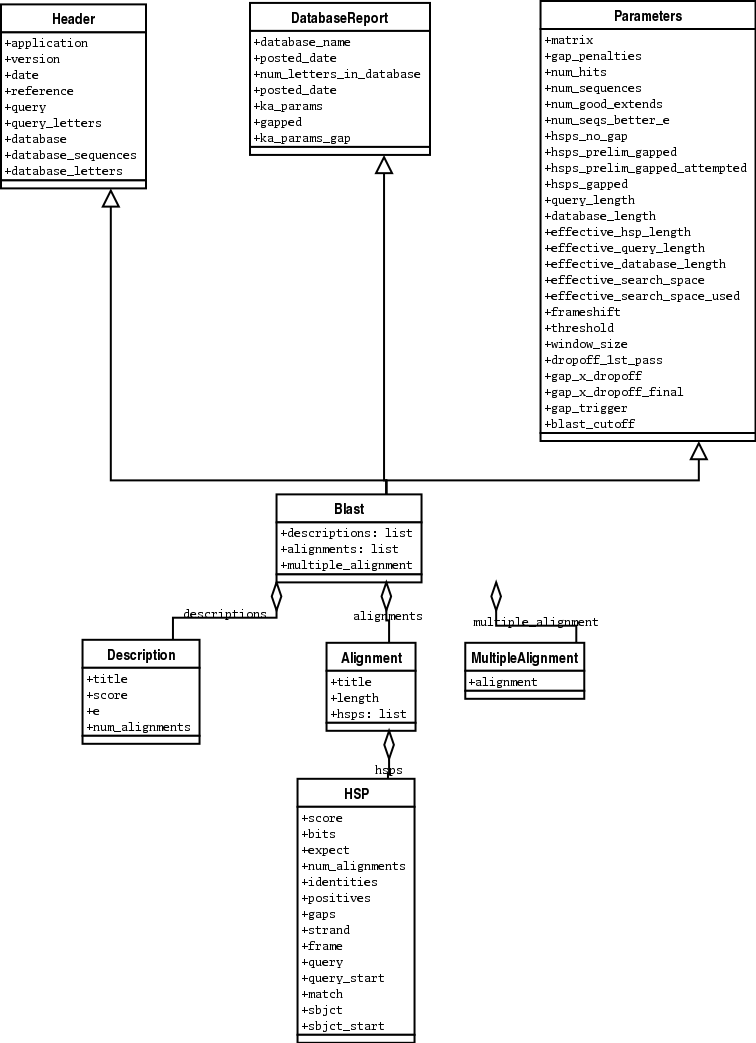
\includegraphics{BlastRecord.png}

PSIBlast 记录类是类似的,但是支持用在迭代器中的rounds方法。PSIBlast类图在这里 {\hyperref[chr07:fig-psiblastrecord]{\emph{7.4}}} 。
\phantomsection\label{chr07:fig-psiblastrecord}
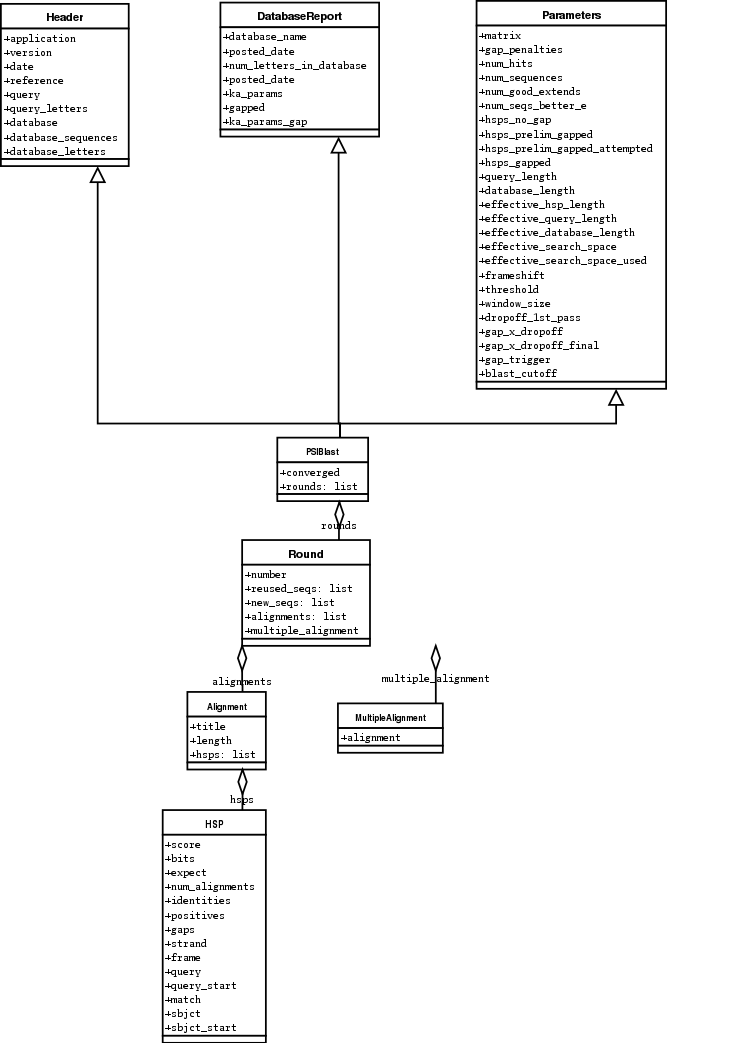
\includegraphics{PSIBlastRecord.png}


\section{7.5  废弃的BLAST 解析器}
\label{chr07:sec-parsing-blast-deprecated}\label{chr07:id5}
老版本的Biopython 有针对纯文本和HTML格式输出结果的解析器。但是经过几年
我们发现维护这些解析器很困难。基本上,任何BLAST输出的任何小改变都会导致
这些解析器失效。所以我们推荐你解析XML格式的BLAST输出结果,就像在
{\hyperref[chr07:sec-parsing-blast]{\emph{7.3}}} 描述的那样。

取决于你使用Biopython的版本,纯文本格式的解析器也许有效也许失效。
用这个解析器的所带来的风险由你自己承担。


\subsection{7.5.1  解析纯文本格式的BLAST输出}
\label{chr07:id6}
纯文本格式的解析器在 \code{Bio.Blast.NCBIStandalone} 。

和xml解析器类似, 我们也需要一个能够传给解析器的文件句柄。这个文件句柄必须
实现了 \code{readline()} 方法 。通常要获得这样文件句柄,既可以用Biopython提供的
\code{blastall} 或 \code{blastpgp} 函数来调用本地的BLAST,或者从命令行运行本地的
BLAST, 并且如下处理:
\DUspan{operator}{}\DUspan{name}{}\DUspan{operator}{}\DUspan{name,builtin}{}\DUspan{punctuation}{}\DUspan{literal,string}{}\DUspan{punctuation}{}
\begin{Verbatim}[commandchars=\\\{\}]
\PYG{g+gp}{\PYGZgt{}\PYGZgt{}\PYGZgt{} }\PYG{n}{result\PYGZus{}handle} \PYG{o}{=} \PYG{n+nb}{open}\PYG{p}{(}\PYG{l+s}{\PYGZdq{}}\PYG{l+s}{my\PYGZus{}file\PYGZus{}of\PYGZus{}blast\PYGZus{}output.txt}\PYG{l+s}{\PYGZdq{}}\PYG{p}{)}
\end{Verbatim}

好了,既然现在得到了个文件句柄(我们称它是 \code{result\_handle} ),
我们已经做好了解析它的准备。按下面的代码来解析:
\DUspan{operator}{}\DUspan{keyword,namespace}{}\DUspan{name,namespace}{}\DUspan{keyword,namespace}{}\DUspan{name}{}\DUspan{operator}{}\DUspan{name}{}\DUspan{operator}{}\DUspan{name}{}\DUspan{operator}{}\DUspan{name}{}\DUspan{punctuation}{}\DUspan{operator}{}\DUspan{name}{}\DUspan{operator}{}\DUspan{name}{}\DUspan{operator}{}\DUspan{name}{}\DUspan{punctuation}{}\DUspan{name}{}\DUspan{punctuation}{}
\begin{Verbatim}[commandchars=\\\{\}]
\PYG{g+gp}{\PYGZgt{}\PYGZgt{}\PYGZgt{} }\PYG{k+kn}{from} \PYG{n+nn}{Bio.Blast} \PYG{k+kn}{import} \PYG{n}{NCBIStandalone}
\PYG{g+gp}{\PYGZgt{}\PYGZgt{}\PYGZgt{} }\PYG{n}{blast\PYGZus{}parser} \PYG{o}{=} \PYG{n}{NCBIStandalone}\PYG{o}{.}\PYG{n}{BlastParser}\PYG{p}{(}\PYG{p}{)}
\PYG{g+gp}{\PYGZgt{}\PYGZgt{}\PYGZgt{} }\PYG{n}{blast\PYGZus{}record} \PYG{o}{=} \PYG{n}{blast\PYGZus{}parser}\PYG{o}{.}\PYG{n}{parse}\PYG{p}{(}\PYG{n}{result\PYGZus{}handle}\PYG{p}{)}
\end{Verbatim}

这样就能把BALST的搜索结果报告解析到Blast记录类中(取决你于你解析的对象,
解析结果可能返回一条 Blast 或者 PSIBlast记录)。这样你就可以从中提取
信息了。在我们的例子里,我们来打印出大于某个阈值的所有比对的一个总结
信息。
\DUspan{operator}{}\DUspan{name}{}\DUspan{operator}{}\DUspan{literal,number,float}{}\DUspan{operator}{}\DUspan{keyword}{}\DUspan{name}{}\DUspan{operator,word}{}\DUspan{name}{}\DUspan{operator}{}\DUspan{name}{}\DUspan{punctuation}{}\DUspan{operator}{}\DUspan{keyword}{}\DUspan{name}{}\DUspan{operator,word}{}\DUspan{name}{}\DUspan{operator}{}\DUspan{name}{}\DUspan{punctuation}{}\DUspan{operator}{}\DUspan{keyword}{}\DUspan{name}{}\DUspan{operator}{}\DUspan{name}{}\DUspan{operator}{}\DUspan{name}{}\DUspan{punctuation}{}\DUspan{operator}{}\DUspan{keyword}{}\DUspan{literal,string}{}\DUspan{operator}{}\DUspan{keyword}{}\DUspan{literal,string}{}\DUspan{punctuation}{}\DUspan{name}{}\DUspan{operator}{}\DUspan{name}{}\DUspan{operator}{}\DUspan{keyword}{}\DUspan{literal,string}{}\DUspan{punctuation}{}\DUspan{name}{}\DUspan{operator}{}\DUspan{name}{}\DUspan{operator}{}\DUspan{keyword}{}\DUspan{literal,string}{}\DUspan{punctuation}{}\DUspan{name}{}\DUspan{operator}{}\DUspan{name}{}\DUspan{operator}{}\DUspan{keyword}{}\DUspan{name}{}\DUspan{operator}{}\DUspan{name}{}\DUspan{punctuation}{}\DUspan{literal,number,integer}{}\DUspan{punctuation}{}\DUspan{literal,number,integer}{}\DUspan{punctuation}{}\DUspan{operator}{}\DUspan{literal,string}{}\DUspan{operator}{}\DUspan{keyword}{}\DUspan{name}{}\DUspan{operator}{}\DUspan{name}{}\DUspan{punctuation}{}\DUspan{literal,number,integer}{}\DUspan{punctuation}{}\DUspan{literal,number,integer}{}\DUspan{punctuation}{}\DUspan{operator}{}\DUspan{literal,string}{}\DUspan{operator}{}\DUspan{keyword}{}\DUspan{name}{}\DUspan{operator}{}\DUspan{name}{}\DUspan{punctuation}{}\DUspan{literal,number,integer}{}\DUspan{punctuation}{}\DUspan{literal,number,integer}{}\DUspan{punctuation}{}\DUspan{operator}{}\DUspan{literal,string}{}
\begin{Verbatim}[commandchars=\\\{\}]
\PYG{g+gp}{\PYGZgt{}\PYGZgt{}\PYGZgt{} }\PYG{n}{E\PYGZus{}VALUE\PYGZus{}THRESH} \PYG{o}{=} \PYG{l+m+mf}{0.04}
\PYG{g+gp}{\PYGZgt{}\PYGZgt{}\PYGZgt{} }\PYG{k}{for} \PYG{n}{alignment} \PYG{o+ow}{in} \PYG{n}{blast\PYGZus{}record}\PYG{o}{.}\PYG{n}{alignments}\PYG{p}{:}
\PYG{g+gp}{... }    \PYG{k}{for} \PYG{n}{hsp} \PYG{o+ow}{in} \PYG{n}{alignment}\PYG{o}{.}\PYG{n}{hsps}\PYG{p}{:}
\PYG{g+gp}{... }        \PYG{k}{if} \PYG{n}{hsp}\PYG{o}{.}\PYG{n}{expect} \PYG{o}{\PYGZlt{}} \PYG{n}{E\PYGZus{}VALUE\PYGZus{}THRESH}\PYG{p}{:}
\PYG{g+gp}{... }            \PYG{k}{print} \PYG{l+s}{\PYGZsq{}}\PYG{l+s}{****Alignment****}\PYG{l+s}{\PYGZsq{}}
\PYG{g+gp}{... }            \PYG{k}{print} \PYG{l+s}{\PYGZsq{}}\PYG{l+s}{sequence:}\PYG{l+s}{\PYGZsq{}}\PYG{p}{,} \PYG{n}{alignment}\PYG{o}{.}\PYG{n}{title}
\PYG{g+gp}{... }            \PYG{k}{print} \PYG{l+s}{\PYGZsq{}}\PYG{l+s}{length:}\PYG{l+s}{\PYGZsq{}}\PYG{p}{,} \PYG{n}{alignment}\PYG{o}{.}\PYG{n}{length}
\PYG{g+gp}{... }            \PYG{k}{print} \PYG{l+s}{\PYGZsq{}}\PYG{l+s}{e value:}\PYG{l+s}{\PYGZsq{}}\PYG{p}{,} \PYG{n}{hsp}\PYG{o}{.}\PYG{n}{expect}
\PYG{g+gp}{... }            \PYG{k}{print} \PYG{n}{hsp}\PYG{o}{.}\PYG{n}{query}\PYG{p}{[}\PYG{l+m+mi}{0}\PYG{p}{:}\PYG{l+m+mi}{75}\PYG{p}{]} \PYG{o}{+} \PYG{l+s}{\PYGZsq{}}\PYG{l+s}{...}\PYG{l+s}{\PYGZsq{}}
\PYG{g+gp}{... }            \PYG{k}{print} \PYG{n}{hsp}\PYG{o}{.}\PYG{n}{match}\PYG{p}{[}\PYG{l+m+mi}{0}\PYG{p}{:}\PYG{l+m+mi}{75}\PYG{p}{]} \PYG{o}{+} \PYG{l+s}{\PYGZsq{}}\PYG{l+s}{...}\PYG{l+s}{\PYGZsq{}}
\PYG{g+gp}{... }            \PYG{k}{print} \PYG{n}{hsp}\PYG{o}{.}\PYG{n}{sbjct}\PYG{p}{[}\PYG{l+m+mi}{0}\PYG{p}{:}\PYG{l+m+mi}{75}\PYG{p}{]} \PYG{o}{+} \PYG{l+s}{\PYGZsq{}}\PYG{l+s}{...}\PYG{l+s}{\PYGZsq{}}
\end{Verbatim}

如果你已经读过 {\hyperref[chr07:sec-parsing-blast]{\emph{7.3}}} 节关于解析XML格式的部分,
你将会发现上面的代码和那个章节的是一样的。一旦你把输出文件解析到记录类中,
你就能处理信息,不管你原来的BLAST输出格式是什么。很赞吧。

好,解析一条记录是不错,那么如果我有一个包含许多记录的BLAST文件 -
我该怎么处理它们呢?好吧,不要害怕,答案就在下个章节中。


\subsection{7.5.2  解析包含多次BLAST结果的纯文本BLAST文件}
\label{chr07:blastblast}
我们可以用BLAST迭代器解析多次结果。为了得到一个迭代器,我们首先需要创建一个解析器,来
解析BLAST的搜索结果报告为Blast记录对象。
\DUspan{operator}{}\DUspan{keyword,namespace}{}\DUspan{name,namespace}{}\DUspan{keyword,namespace}{}\DUspan{name}{}\DUspan{operator}{}\DUspan{name}{}\DUspan{operator}{}\DUspan{name}{}\DUspan{operator}{}\DUspan{name}{}\DUspan{punctuation}{}
\begin{Verbatim}[commandchars=\\\{\}]
\PYG{g+gp}{\PYGZgt{}\PYGZgt{}\PYGZgt{} }\PYG{k+kn}{from} \PYG{n+nn}{Bio.Blast} \PYG{k+kn}{import} \PYG{n}{NCBIStandalone}
\PYG{g+gp}{\PYGZgt{}\PYGZgt{}\PYGZgt{} }\PYG{n}{blast\PYGZus{}parser} \PYG{o}{=} \PYG{n}{NCBIStandalone}\PYG{o}{.}\PYG{n}{BlastParser}\PYG{p}{(}\PYG{p}{)}
\end{Verbatim}

然后,我们假定我们有一个连接到一大堆blast记录的文件句柄,我们把这个文件句柄
叫做  \code{result\_handle} 。 怎么得到一个文件句柄在上面blast解析章节有详细
描述。

好了,我们现在有了一个解析器和一个文件句柄,我们可以用以下命令来创建
一个迭代器。
\DUspan{operator}{}\DUspan{name}{}\DUspan{operator}{}\DUspan{name}{}\DUspan{operator}{}\DUspan{name}{}\DUspan{punctuation}{}\DUspan{name}{}\DUspan{punctuation}{}\DUspan{name}{}\DUspan{punctuation}{}
\begin{Verbatim}[commandchars=\\\{\}]
\PYG{g+gp}{\PYGZgt{}\PYGZgt{}\PYGZgt{} }\PYG{n}{blast\PYGZus{}iterator} \PYG{o}{=} \PYG{n}{NCBIStandalone}\PYG{o}{.}\PYG{n}{Iterator}\PYG{p}{(}\PYG{n}{result\PYGZus{}handle}\PYG{p}{,} \PYG{n}{blast\PYGZus{}parser}\PYG{p}{)}
\end{Verbatim}

第二个参数,解析器,是可选的。如果我们没有提供一个解析器,那么迭代器将会
一次返回一个原始的BLAST搜索结果。

现在我们已经有了个迭代器,就可以开始通过 \code{next()} 方法来获取BLAST
记录(由我们的解析器产生)。
\DUspan{operator}{}\DUspan{name}{}\DUspan{operator}{}\DUspan{name}{}\DUspan{operator}{}\DUspan{name}{}\DUspan{punctuation}{}
\begin{Verbatim}[commandchars=\\\{\}]
\PYG{g+gp}{\PYGZgt{}\PYGZgt{}\PYGZgt{} }\PYG{n}{blast\PYGZus{}record} \PYG{o}{=} \PYG{n}{blast\PYGZus{}iterator}\PYG{o}{.}\PYG{n}{next}\PYG{p}{(}\PYG{p}{)}
\end{Verbatim}

每次调用next都会返回一条我们能处理的新记录。现在我们可以遍历所有记录,并打印一
个我们最爱、漂亮的、简洁的BLAST记录报告。
\DUspan{operator}{}\DUspan{keyword}{}\DUspan{name}{}\DUspan{operator,word}{}\DUspan{name}{}\DUspan{punctuation}{}\DUspan{operator}{}\DUspan{name}{}\DUspan{operator}{}\DUspan{literal,number,float}{}\DUspan{operator}{}\DUspan{keyword}{}\DUspan{name}{}\DUspan{operator,word}{}\DUspan{name}{}\DUspan{operator}{}\DUspan{name}{}\DUspan{punctuation}{}\DUspan{operator}{}\DUspan{keyword}{}\DUspan{name}{}\DUspan{operator,word}{}\DUspan{name}{}\DUspan{operator}{}\DUspan{name}{}\DUspan{punctuation}{}\DUspan{operator}{}\DUspan{keyword}{}\DUspan{name}{}\DUspan{operator}{}\DUspan{name}{}\DUspan{operator}{}\DUspan{name}{}\DUspan{punctuation}{}\DUspan{operator}{}\DUspan{keyword}{}\DUspan{literal,string}{}\DUspan{operator}{}\DUspan{keyword}{}\DUspan{literal,string}{}\DUspan{punctuation}{}\DUspan{name}{}\DUspan{operator}{}\DUspan{name}{}\DUspan{operator}{}\DUspan{keyword}{}\DUspan{literal,string}{}\DUspan{punctuation}{}\DUspan{name}{}\DUspan{operator}{}\DUspan{name}{}\DUspan{operator}{}\DUspan{keyword}{}\DUspan{literal,string}{}\DUspan{punctuation}{}\DUspan{name}{}\DUspan{operator}{}\DUspan{name}{}\DUspan{operator}{}\DUspan{keyword}{}\DUspan{name,builtin}{}\DUspan{punctuation}{}\DUspan{name}{}\DUspan{operator}{}\DUspan{name}{}\DUspan{punctuation}{}\DUspan{operator}{}\DUspan{literal,number,integer}{}\DUspan{punctuation}{}\DUspan{operator}{}\DUspan{name}{}\DUspan{operator}{}\DUspan{literal,string}{}\DUspan{operator}{}\DUspan{keyword}{}\DUspan{punctuation}{}\DUspan{operator}{}\DUspan{name}{}\DUspan{operator}{}\DUspan{literal,string}{}\DUspan{operator}{}\DUspan{keyword}{}\DUspan{name}{}\DUspan{operator}{}\DUspan{name}{}\DUspan{punctuation}{}\DUspan{literal,number,integer}{}\DUspan{punctuation}{}\DUspan{literal,number,integer}{}\DUspan{punctuation}{}\DUspan{operator}{}\DUspan{name}{}\DUspan{operator}{}\DUspan{keyword}{}\DUspan{name}{}\DUspan{operator}{}\DUspan{name}{}\DUspan{punctuation}{}\DUspan{literal,number,integer}{}\DUspan{punctuation}{}\DUspan{literal,number,integer}{}\DUspan{punctuation}{}\DUspan{operator}{}\DUspan{name}{}\DUspan{operator}{}\DUspan{keyword}{}\DUspan{name}{}\DUspan{operator}{}\DUspan{name}{}\DUspan{punctuation}{}\DUspan{literal,number,integer}{}\DUspan{punctuation}{}\DUspan{literal,number,integer}{}\DUspan{punctuation}{}\DUspan{operator}{}\DUspan{name}{}
\begin{Verbatim}[commandchars=\\\{\}]
\PYG{g+gp}{\PYGZgt{}\PYGZgt{}\PYGZgt{} }\PYG{k}{for} \PYG{n}{blast\PYGZus{}record} \PYG{o+ow}{in} \PYG{n}{blast\PYGZus{}iterator}\PYG{p}{:}
\PYG{g+gp}{... }    \PYG{n}{E\PYGZus{}VALUE\PYGZus{}THRESH} \PYG{o}{=} \PYG{l+m+mf}{0.04}
\PYG{g+gp}{... }    \PYG{k}{for} \PYG{n}{alignment} \PYG{o+ow}{in} \PYG{n}{blast\PYGZus{}record}\PYG{o}{.}\PYG{n}{alignments}\PYG{p}{:}
\PYG{g+gp}{... }        \PYG{k}{for} \PYG{n}{hsp} \PYG{o+ow}{in} \PYG{n}{alignment}\PYG{o}{.}\PYG{n}{hsps}\PYG{p}{:}
\PYG{g+gp}{... }            \PYG{k}{if} \PYG{n}{hsp}\PYG{o}{.}\PYG{n}{expect} \PYG{o}{\PYGZlt{}} \PYG{n}{E\PYGZus{}VALUE\PYGZus{}THRESH}\PYG{p}{:}
\PYG{g+gp}{... }                \PYG{k}{print} \PYG{l+s}{\PYGZsq{}}\PYG{l+s}{****Alignment****}\PYG{l+s}{\PYGZsq{}}
\PYG{g+gp}{... }                \PYG{k}{print} \PYG{l+s}{\PYGZsq{}}\PYG{l+s}{sequence:}\PYG{l+s}{\PYGZsq{}}\PYG{p}{,} \PYG{n}{alignment}\PYG{o}{.}\PYG{n}{title}
\PYG{g+gp}{... }                \PYG{k}{print} \PYG{l+s}{\PYGZsq{}}\PYG{l+s}{length:}\PYG{l+s}{\PYGZsq{}}\PYG{p}{,} \PYG{n}{alignment}\PYG{o}{.}\PYG{n}{length}
\PYG{g+gp}{... }                \PYG{k}{print} \PYG{l+s}{\PYGZsq{}}\PYG{l+s}{e value:}\PYG{l+s}{\PYGZsq{}}\PYG{p}{,} \PYG{n}{hsp}\PYG{o}{.}\PYG{n}{expect}
\PYG{g+gp}{... }                \PYG{k}{if} \PYG{n+nb}{len}\PYG{p}{(}\PYG{n}{hsp}\PYG{o}{.}\PYG{n}{query}\PYG{p}{)} \PYG{o}{\PYGZgt{}} \PYG{l+m+mi}{75}\PYG{p}{:}
\PYG{g+gp}{... }                    \PYG{n}{dots} \PYG{o}{=} \PYG{l+s}{\PYGZsq{}}\PYG{l+s}{...}\PYG{l+s}{\PYGZsq{}}
\PYG{g+gp}{... }                \PYG{k}{else}\PYG{p}{:}
\PYG{g+gp}{... }                    \PYG{n}{dots} \PYG{o}{=} \PYG{l+s}{\PYGZsq{}}\PYG{l+s}{\PYGZsq{}}
\PYG{g+gp}{... }                \PYG{k}{print} \PYG{n}{hsp}\PYG{o}{.}\PYG{n}{query}\PYG{p}{[}\PYG{l+m+mi}{0}\PYG{p}{:}\PYG{l+m+mi}{75}\PYG{p}{]} \PYG{o}{+} \PYG{n}{dots}
\PYG{g+gp}{... }                \PYG{k}{print} \PYG{n}{hsp}\PYG{o}{.}\PYG{n}{match}\PYG{p}{[}\PYG{l+m+mi}{0}\PYG{p}{:}\PYG{l+m+mi}{75}\PYG{p}{]} \PYG{o}{+} \PYG{n}{dots}
\PYG{g+gp}{... }                \PYG{k}{print} \PYG{n}{hsp}\PYG{o}{.}\PYG{n}{sbjct}\PYG{p}{[}\PYG{l+m+mi}{0}\PYG{p}{:}\PYG{l+m+mi}{75}\PYG{p}{]} \PYG{o}{+} \PYG{n}{dots}
\end{Verbatim}

迭代器允许你处理很多blast记录而不出现内存不足的问题。因为,它使一次处理
一个记录。我曾经用大处理过一个非常巨大的文件,没有出过任何问题。


\subsection{7.5.3  在巨大的BLAST纯文本文件中发现不对的记录}
\label{chr07:id7}
当我开始解析一个巨大的blast 文件,有时候会碰到一个郁闷的问题就是解析器以一个
ValueError异常终止了。这是个严肃的问题。因为你无法分辨导致ValueError异常的是
解析器的问题还是BLAST的问题。更加糟糕是,你不知道在哪一行解析器失效了。所以,
你不能忽略这个错误。不然,可能会忽视一个重要的数据。

我们以前必须写一些小脚本来解决这个问题。不过,现在 \code{Bio.Blast} 模块包含了
\code{BlastErrorParser} ,可以更加简单地来解决这个问题。 \code{BlastErrorParser}
和常规的 \code{BlastParser} 类似,但是它加了特别一层来捕获由解析器产生的ValueErrors
异常,并尝试来诊断这些错误。

让我们来看看怎样用这个解析器 - 首先我们定义我们准备解析的文件和报告错误情况的
输出文件。
\DUspan{operator}{}\DUspan{keyword,namespace}{}\DUspan{name,namespace}{}\DUspan{operator}{}\DUspan{name}{}\DUspan{operator}{}\DUspan{name}{}\DUspan{operator}{}\DUspan{name}{}\DUspan{operator}{}\DUspan{name}{}\DUspan{punctuation}{}\DUspan{name}{}\DUspan{operator}{}\DUspan{name}{}\DUspan{punctuation}{}\DUspan{literal,string}{}\DUspan{punctuation}{}\DUspan{literal,string}{}\DUspan{punctuation}{}\DUspan{operator}{}\DUspan{name}{}\DUspan{operator}{}\DUspan{name}{}\DUspan{operator}{}\DUspan{name}{}\DUspan{operator}{}\DUspan{name}{}\DUspan{punctuation}{}\DUspan{name}{}\DUspan{operator}{}\DUspan{name}{}\DUspan{punctuation}{}\DUspan{literal,string}{}\DUspan{punctuation}{}\DUspan{literal,string}{}\DUspan{punctuation}{}
\begin{Verbatim}[commandchars=\\\{\}]
\PYG{g+gp}{\PYGZgt{}\PYGZgt{}\PYGZgt{} }\PYG{k+kn}{import} \PYG{n+nn}{os}
\PYG{g+gp}{\PYGZgt{}\PYGZgt{}\PYGZgt{} }\PYG{n}{blast\PYGZus{}file} \PYG{o}{=} \PYG{n}{os}\PYG{o}{.}\PYG{n}{path}\PYG{o}{.}\PYG{n}{join}\PYG{p}{(}\PYG{n}{os}\PYG{o}{.}\PYG{n}{getcwd}\PYG{p}{(}\PYG{p}{)}\PYG{p}{,} \PYG{l+s}{\PYGZdq{}}\PYG{l+s}{blast\PYGZus{}out}\PYG{l+s}{\PYGZdq{}}\PYG{p}{,} \PYG{l+s}{\PYGZdq{}}\PYG{l+s}{big\PYGZus{}blast.out}\PYG{l+s}{\PYGZdq{}}\PYG{p}{)}
\PYG{g+gp}{\PYGZgt{}\PYGZgt{}\PYGZgt{} }\PYG{n}{error\PYGZus{}file} \PYG{o}{=} \PYG{n}{os}\PYG{o}{.}\PYG{n}{path}\PYG{o}{.}\PYG{n}{join}\PYG{p}{(}\PYG{n}{os}\PYG{o}{.}\PYG{n}{getcwd}\PYG{p}{(}\PYG{p}{)}\PYG{p}{,} \PYG{l+s}{\PYGZdq{}}\PYG{l+s}{blast\PYGZus{}out}\PYG{l+s}{\PYGZdq{}}\PYG{p}{,} \PYG{l+s}{\PYGZdq{}}\PYG{l+s}{big\PYGZus{}blast.problems}\PYG{l+s}{\PYGZdq{}}\PYG{p}{)}
\end{Verbatim}

现在我们想要一个  \code{BlastErrorParser} :
\DUspan{operator}{}\DUspan{keyword,namespace}{}\DUspan{name,namespace}{}\DUspan{keyword,namespace}{}\DUspan{name}{}\DUspan{operator}{}\DUspan{name}{}\DUspan{operator}{}\DUspan{name,builtin}{}\DUspan{punctuation}{}\DUspan{name}{}\DUspan{punctuation}{}\DUspan{literal,string}{}\DUspan{punctuation}{}\DUspan{operator}{}\DUspan{name}{}\DUspan{operator}{}\DUspan{name}{}\DUspan{operator}{}\DUspan{name}{}\DUspan{punctuation}{}\DUspan{name}{}\DUspan{punctuation}{}
\begin{Verbatim}[commandchars=\\\{\}]
\PYG{g+gp}{\PYGZgt{}\PYGZgt{}\PYGZgt{} }\PYG{k+kn}{from} \PYG{n+nn}{Bio.Blast} \PYG{k+kn}{import} \PYG{n}{NCBIStandalone}
\PYG{g+gp}{\PYGZgt{}\PYGZgt{}\PYGZgt{} }\PYG{n}{error\PYGZus{}handle} \PYG{o}{=} \PYG{n+nb}{open}\PYG{p}{(}\PYG{n}{error\PYGZus{}file}\PYG{p}{,} \PYG{l+s}{\PYGZdq{}}\PYG{l+s}{w}\PYG{l+s}{\PYGZdq{}}\PYG{p}{)}
\PYG{g+gp}{\PYGZgt{}\PYGZgt{}\PYGZgt{} }\PYG{n}{blast\PYGZus{}error\PYGZus{}parser} \PYG{o}{=} \PYG{n}{NCBIStandalone}\PYG{o}{.}\PYG{n}{BlastErrorParser}\PYG{p}{(}\PYG{n}{error\PYGZus{}handle}\PYG{p}{)}
\end{Verbatim}

注意,解析器有个关于文件句柄的可选参数。如果传递了这个参数,那么解析器就会
把产生ValueError异常的记录写到这个文件句柄中。不然的话,这些错误记录就不会
被记录下来。

现在,我们可以像用常规的blast解析器一样地用 \code{BlastErrorParser} 。
特别的是,我们也许想要一个一次读入一个记录的迭代器并用 \code{BlastErrorParser}
来解析它。
\DUspan{operator}{}\DUspan{name}{}\DUspan{operator}{}\DUspan{name,builtin}{}\DUspan{punctuation}{}\DUspan{name}{}\DUspan{punctuation}{}\DUspan{operator}{}\DUspan{name}{}\DUspan{operator}{}\DUspan{name}{}\DUspan{operator}{}\DUspan{name}{}\DUspan{punctuation}{}\DUspan{name}{}\DUspan{punctuation}{}\DUspan{name}{}\DUspan{punctuation}{}
\begin{Verbatim}[commandchars=\\\{\}]
\PYG{g+gp}{\PYGZgt{}\PYGZgt{}\PYGZgt{} }\PYG{n}{result\PYGZus{}handle} \PYG{o}{=} \PYG{n+nb}{open}\PYG{p}{(}\PYG{n}{blast\PYGZus{}file}\PYG{p}{)}
\PYG{g+gp}{\PYGZgt{}\PYGZgt{}\PYGZgt{} }\PYG{n}{iterator} \PYG{o}{=} \PYG{n}{NCBIStandalone}\PYG{o}{.}\PYG{n}{Iterator}\PYG{p}{(}\PYG{n}{result\PYGZus{}handle}\PYG{p}{,} \PYG{n}{blast\PYGZus{}error\PYGZus{}parser}\PYG{p}{)}
\end{Verbatim}

我们可以一次读一个记录,并且我们现在可以捕获并处理那些因为Blast引起的、
不是解析器本身导致的错误。
\DUspan{operator}{}\DUspan{keyword}{}\DUspan{punctuation}{}\DUspan{operator}{}\DUspan{name}{}\DUspan{operator}{}\DUspan{name}{}\DUspan{operator}{}\DUspan{name}{}\DUspan{punctuation}{}\DUspan{operator}{}\DUspan{keyword}{}\DUspan{name}{}\DUspan{operator}{}\DUspan{name}{}\DUspan{punctuation}{}\DUspan{name}{}\DUspan{punctuation}{}\DUspan{operator}{}\DUspan{keyword}{}\DUspan{literal,string}{}\DUspan{literal,string,interpol}{}\DUspan{literal,string}{}\DUspan{operator}{}\DUspan{name}{}\DUspan{punctuation}{}\DUspan{literal,number,integer}{}\DUspan{punctuation}{}
\begin{Verbatim}[commandchars=\\\{\}]
\PYG{g+gp}{\PYGZgt{}\PYGZgt{}\PYGZgt{} }\PYG{k}{try}\PYG{p}{:}
\PYG{g+gp}{... }    \PYG{n}{next\PYGZus{}record} \PYG{o}{=} \PYG{n}{iterator}\PYG{o}{.}\PYG{n}{next}\PYG{p}{(}\PYG{p}{)}
\PYG{g+gp}{... }\PYG{k}{except} \PYG{n}{NCBIStandalone}\PYG{o}{.}\PYG{n}{LowQualityBlastError}\PYG{p}{,} \PYG{n}{info}\PYG{p}{:}
\PYG{g+gp}{... }    \PYG{k}{print} \PYG{l+s}{\PYGZdq{}}\PYG{l+s}{LowQualityBlastError detected in id }\PYG{l+s+si}{\PYGZpc{}s}\PYG{l+s}{\PYGZdq{}} \PYG{o}{\PYGZpc{}} \PYG{n}{info}\PYG{p}{[}\PYG{l+m+mi}{1}\PYG{p}{]}
\end{Verbatim}

\code{.next()} 方法通常被 \code{for} 循环间接地调用。现在, \code{BlastErrorParser}
能够捕获如下的错误:
\begin{itemize}
\item {} 
\code{ValueError} - 这就是和常规BlastParser产生的一样的错误。这个错误产生
是因为解析器不能解析某个文件。通常是因为解析器有bug, 或者是
因为你使用解析器的版本和你BLAST命令的版本不一致。

\item {} 
\code{LowQualityBlastError} - 当Blast一条低质量的序列时(比如,一条
只有1个核苷酸的短序列),似乎Blast会终止并屏蔽掉整个序列,所有就没有什么可以
解析了。 这种情况下,Blast就会产生一个不完整的报告导致解析器出现ValueError
错误。 \code{LowQualityBlastError} 错误在这种情况下产生。这个错误返回如下
信息:
\begin{itemize}
\item {} 
\code{item{[}0{]}} – The error message

\item {} 
\code{item{[}0{]}} - 错误消息

\item {} 
\code{item{[}1{]}} – The id of the input record that caused the error.
This is really useful if you want to record all of the records
that are causing problems.

\item {} 
\code{item{[}1{]}} - 导致错误产生的输入记录id。如果你想记录所有导致问题
记录的时候很有用。

\end{itemize}

\end{itemize}

就像上面提到的那样,BlastErrorParser 将会把有问题的记录写到指定的{}`{}`error\_handle{}`{}`。
然后,你可以排查这些有问题记录。你可以针对某条记录来调试解析器,或者找到
你运行blast中的问题。无论哪种方式,这些都是有用的经验。

希望 \code{BlastErrorParser} 能帮你更简单的调试和处理一些数据巨大的Blast 文件。


\section{7.6  处理PSI-BLAST}
\label{chr07:psi-blast}
你可以通过 \code{Bio.Blast.Applications} 模块中的包装函数来运行单机版本的PSI-BLAST
(老版本的NCBI命令工具行 \code{blastpgp} 或者它的替代程序 \code{psiblast} )。

在写这篇指南的时候,没有迹象表明NCBI将会支持通过internet来进行PSI-BLAST
搜索。

请注意 \code{Bio.Blast.NCBIXML} 解析器能读入并解析当前版本PSI-BLAST的、XML格式的
输出,但是像哪条序列在每个迭代循环中是新的还是复用的信息在XML格式输出中是没有的。
如果,你需要这些信息你应该用纯文本输出和 \code{Bio.Blast.NCBIStandalone} 模块的
\code{PSIBlastParser} 。


\section{7.7  处理 RPS-BLAST}
\label{chr07:rps-blast}
你可以通过 \code{Bio.Blast.Applications} 模块中的包装函数来运行单机版本的RPS-BLAST
(或者老版本的NCBI命令工具行 \code{rpsblast} 或者同样名字的替代程序 )。

在写这篇指南的时候,没有迹象表明NCBI将会支持通过internet来进行RPS-BLAST
搜索

你可以通过 \code{Bio.Blast.NCBIXML} 这个解析器来读入并解析当前版本的RPS-BLAST的
XML格式的输出。


\chapter{第8章  BLAST和其他序列搜索工具(\emph{实验性质的代码})}
\label{chr08:chapter-searchio}\label{chr08:blast}\label{chr08::doc}
\emph{WARNING}: 这章教程介绍了Biopython中一个 \emph{实验的} 模块。它正在被加入到
Biopython中,并且以一个预尾期的状态整理到教程当中,这样在我们发布稳定版
的之前可以收到一系列的反馈和并作改进。那时有些细节可能会改变,并且用到
当前 \code{Bio.SearchIO} 模块的脚本也需要更新。切记!为了与NCBI BLAST有关的
代码可以稳定工作,请继续使用第 {\hyperref[chr07:chapter-blast]{\emph{7}}} 章介绍的Bio.Blast。

生物序列的鉴定是生物信息工作的主要部分。有几个工具像BLAST(可能是最流行
的),FASTA ,HMMER还有许多其它的都有这个功能,每个工具都有独特的算法和
途径。一般来说,这些工具都是用你的序列在数据库中搜索可能的匹配。随着序列
数量的增加(匹配数也会随之增加),将会有成百上千的可能匹配,解析这些结果
无疑变得越来越困难。理所当然,人工解析搜索结果变得不可能。而且你可能会同
时用几种不同的搜索工具,每种工具都有独特的统计方法、规则和输出格式。可以
想象,同时用多种工具搜索多条序列是多么恐怖的事。

我们对此非常了解,所以我们在Biopython构建了 \code{Bio.SearchIO} 亚模块。\code{Bio.SearchIO} 模块使从搜索结果中提取信息变得简单,并且可以处理不同工具
的不同标准和规则。\code{SearchIO} 和BioPerl中模块名称一致。

在本章中,我们将学习 \code{Bio.SearchIO} 的主要功能,了解它可以做什么。我
们将使用两个主要的搜索工具:BLAST和FASTA。它们只是用来阐明思路,你可以轻
易地把工作流程应用到 \code{Bio.SearchIO} 支持的其他工具中。欢迎你使用我们将要
用到的搜索结果文件。BLAST搜索结果文件可以在
\href{http://biopython.org/SRC/Tests/Tutorial/my\_blast.xml}{这里} 下载。
BLAT输出结果文件可以在
\href{http://biopython.org/SRC/Tests/Tutorial/my\_blat.psl}{这里} 下载。两个结果
文件都是用下面这条序列搜索产生的:
\DUspan{operator}{}\DUspan{name}{}\DUspan{name}{}
\begin{Verbatim}[commandchars=\\\{\}]
\textgreater{}mystery\_seq
CCCTCTACAGGGAAGCGCTTTCTGTTGTCTGAAAGAAAAGAAAGTGCTTCCTTTTAGAGGG
\end{Verbatim}

BLAST的XML结果是用 \code{blastn} 搜索NCBI的 \code{refseq\_rna} 数据库得到的。对于
BLAT,数据库是2009年2月份的 \code{hg19} 人类基因组草图,输出格式是PSL。

我们从 \code{Bio.SearchIO} 的对象模型的介绍开始。这个模型代表你的搜索结果,因
此它是 \code{Bio.SearchIO} 的核心。然后,我们会介绍 \code{Bio.SearchIO} 常用的主要
功能。

现在一切就绪,让我们开始第一步:介绍核心对象模型。


\section{8.1  SearchIO对象模型}
\label{chr08:searchio}
尽管多数搜索工具的输出风格极为不同,但是它们蕴含的理念很相似:
\begin{itemize}
\item {} 
输出文件可能包含一条或更多的搜索查询的结果。

\item {} 
在每次查询中,你会在给定的数据库中得到一个或更多的hit(命中)。

\item {} 
在每个hit中,你会得到一个或更多包含query(查询)序列和数据库序列实际比对的区域。

\item {} 
一些工具如BLAT和Exonerate可能会把这些区域分成几个比对片段(或在BLAT中
称为区块,在Exonerate中称为可能外显子)。这并不是很常见,像BLAST和
HMMER就不这么做。

\end{itemize}

知道这些共性之后,我们决定把它们作为创造 \code{Bio.SearchIO} 对象模型的基础。对
象模型是Python对象组成的嵌套分级系统,每个对象都代表一个上面列出的概念。这些对
象是:
\begin{itemize}
\item {} 
\code{QueryResult},代表单个搜索查询。

\item {} 
\code{Hit},代表单个的数据库hit。\code{Hit} 对象包含在 \code{QueryResult} 中,
每个 \code{QueryResult} 中有0个或多个 \code{Hit} 对象。

\item {} 
\code{HSP} (high-scoring pair(高分片段)),代表query和hit序列中有
意义比对的区域。\code{HSP} 对象包含在 \code{Hit} 对象中,而且每个 \code{Hit} 有一个
或更多的 \code{HSP} 对象。

\item {} 
\code{HSPFragment},代表query和hit序列中单个的邻近比对。 \code{HSPFragment}
对象包含在 \code{HSP} 对象中。多数的搜索工具如BLAST和HMMER把 \code{HSP} 和
\code{HSPFragment} 合并,因为一个 \code{HSP} 只含有一个 \code{HSPFragment}。但是
像BLAT和Exonerate会产生含有多个 \code{HSPFragment} 的 \code{HSP} 。似乎有些困
惑?不要紧,稍后我们将详细介绍这两个对象。

\end{itemize}

这四个对象是当你用 \code{Bio.SearchIO} 会碰到的。 \code{Bio.SearchIO} 四
个主要方法: \code{read} ,\code{parse},\code{index} 或 \code{index\_db} 中任意一个都可
以产生这四个对象。这些方法的会在后面的部分详细介绍。这部分只会用到 \code{read} 和
\code{parse} ,这两个方法和 \code{Bio.SeqIO} 以及 \code{Bio.AlignIO} 中的 \code{read} 和 \code{parse} 方法功
能相似:
\begin{itemize}
\item {} 
\code{read} 用于单query对输出文件进行搜索并且返回一个 \code{QueryResult} 对象。

\item {} 
\code{parse} 用于多query对输出文件进行搜索并且返回一个可以yield \code{QueryResult} 对象的generator。

\end{itemize}

完成这些之后,让我们开始学习每个 \code{Bio.SearchIO} 对象,从 \code{QueryResult} 开始。


\subsection{8.1.1  QueryResult}
\label{chr08:queryresult}
\code{QueryResult},代表单query搜索,每个 \code{QueryResult} 中有0个或多个 \code{Hit} 对象。我们来看看BLAST文件是什么样的:
\DUspan{operator}{}\DUspan{keyword,namespace}{}\DUspan{name,namespace}{}\DUspan{keyword,namespace}{}\DUspan{name}{}\DUspan{operator}{}\DUspan{name}{}\DUspan{operator}{}\DUspan{name}{}\DUspan{operator}{}\DUspan{name}{}\DUspan{punctuation}{}\DUspan{literal,string}{}\DUspan{punctuation}{}\DUspan{literal,string}{}\DUspan{punctuation}{}\DUspan{operator}{}\DUspan{keyword}{}\DUspan{name}{}\DUspan{name}{}\DUspan{punctuation}{}\DUspan{name}{}\DUspan{punctuation}{}\DUspan{literal,number,float}{}\DUspan{operator}{}\DUspan{literal,number,integer}{}\DUspan{operator}{}\DUspan{punctuation}{}\DUspan{name}{}\DUspan{punctuation}{}\DUspan{literal,number,integer}{}\DUspan{punctuation}{}\DUspan{literal,number,integer}{}\DUspan{punctuation}{}\DUspan{name}{}\DUspan{name}{}\DUspan{punctuation}{}\DUspan{name}{}\DUspan{name}{}\DUspan{punctuation}{}\DUspan{operator}{}\DUspan{operator}{}\DUspan{operator}{}\DUspan{comment}{}\DUspan{operator}{}\DUspan{operator}{}\DUspan{operator}{}\DUspan{literal,number,integer}{}\DUspan{literal,number,integer}{}\DUspan{name}{}\DUspan{operator}{}\DUspan{literal,number,integer}{}\DUspan{operator}{}\DUspan{name}{}\DUspan{operator}{}\DUspan{name}{}\DUspan{operator}{}\DUspan{literal,number,integer}{}\DUspan{operator}{}\DUspan{name}{}\DUspan{name}{}\DUspan{name}{}\DUspan{literal,number,float}{}\DUspan{operator}{}\DUspan{literal,number,integer}{}\DUspan{literal,number,integer}{}\DUspan{name}{}\DUspan{operator}{}\DUspan{literal,number,integer}{}\DUspan{operator}{}\DUspan{name}{}\DUspan{operator}{}\DUspan{name}{}\DUspan{operator}{}\DUspan{literal,number,integer}{}\DUspan{operator}{}\DUspan{name}{}\DUspan{name}{}\DUspan{name}{}\DUspan{operator}{}\DUspan{literal,number,integer}{}\DUspan{literal,number,integer}{}\DUspan{name}{}\DUspan{operator}{}\DUspan{literal,number,integer}{}\DUspan{operator}{}\DUspan{name}{}\DUspan{operator}{}\DUspan{name}{}\DUspan{operator}{}\DUspan{literal,number,integer}{}\DUspan{operator}{}\DUspan{name}{}\DUspan{name}{}\DUspan{name}{}\DUspan{operator}{}\DUspan{literal,number,integer}{}\DUspan{literal,number,integer}{}\DUspan{name}{}\DUspan{operator}{}\DUspan{literal,number,integer}{}\DUspan{operator}{}\DUspan{name}{}\DUspan{operator}{}\DUspan{name}{}\DUspan{operator}{}\DUspan{literal,number,integer}{}\DUspan{operator}{}\DUspan{name}{}\DUspan{name}{}\DUspan{name}{}\DUspan{operator}{}\DUspan{literal,number,integer}{}\DUspan{literal,number,integer}{}\DUspan{name}{}\DUspan{operator}{}\DUspan{literal,number,integer}{}\DUspan{operator}{}\DUspan{name}{}\DUspan{operator}{}\DUspan{name}{}\DUspan{operator}{}\DUspan{literal,number,integer}{}\DUspan{operator}{}\DUspan{name}{}\DUspan{name}{}\DUspan{name}{}\DUspan{operator}{}\DUspan{literal,number,integer}{}\DUspan{literal,number,integer}{}\DUspan{name}{}\DUspan{operator}{}\DUspan{literal,number,integer}{}\DUspan{operator}{}\DUspan{name}{}\DUspan{operator}{}\DUspan{name}{}\DUspan{operator}{}\DUspan{literal,number,integer}{}\DUspan{operator}{}\DUspan{name}{}\DUspan{name}{}\DUspan{name}{}\DUspan{literal,number,float}{}\DUspan{operator}{}\DUspan{literal,number,integer}{}\DUspan{literal,number,integer}{}\DUspan{name}{}\DUspan{operator}{}\DUspan{literal,number,integer}{}\DUspan{operator}{}\DUspan{name}{}\DUspan{operator}{}\DUspan{name}{}\DUspan{operator}{}\DUspan{literal,number,integer}{}\DUspan{operator}{}\DUspan{name}{}\DUspan{name}{}\DUspan{name}{}\DUspan{literal,number,float}{}\DUspan{operator}{}\DUspan{literal,number,integer}{}\DUspan{literal,number,integer}{}\DUspan{name}{}\DUspan{operator}{}\DUspan{literal,number,integer}{}\DUspan{operator}{}\DUspan{name}{}\DUspan{operator}{}\DUspan{name}{}\DUspan{operator}{}\DUspan{literal,number,integer}{}\DUspan{operator}{}\DUspan{name}{}\DUspan{name}{}\DUspan{name}{}\DUspan{operator}{}\DUspan{literal,number,integer}{}\DUspan{literal,number,integer}{}\DUspan{name}{}\DUspan{operator}{}\DUspan{literal,number,integer}{}\DUspan{operator}{}\DUspan{name}{}\DUspan{operator}{}\DUspan{name}{}\DUspan{operator}{}\DUspan{literal,number,integer}{}\DUspan{operator}{}\DUspan{name}{}\DUspan{name}{}\DUspan{name}{}\DUspan{literal,number,float}{}\DUspan{operator}{}\DUspan{literal,number,integer}{}\DUspan{literal,number,integer}{}\DUspan{name}{}\DUspan{operator}{}\DUspan{literal,number,integer}{}\DUspan{operator}{}\DUspan{name}{}\DUspan{operator}{}\DUspan{name}{}\DUspan{operator}{}\DUspan{literal,number,integer}{}\DUspan{operator}{}\DUspan{name}{}\DUspan{name}{}\DUspan{name}{}\DUspan{operator}{}\DUspan{literal,number,integer}{}\DUspan{literal,number,integer}{}\DUspan{name}{}\DUspan{operator}{}\DUspan{literal,number,integer}{}\DUspan{operator}{}\DUspan{name}{}\DUspan{operator}{}\DUspan{name}{}\DUspan{operator}{}\DUspan{literal,number,integer}{}\DUspan{operator}{}\DUspan{name}{}\DUspan{name}{}\DUspan{name}{}\DUspan{operator}{}\DUspan{literal,number,integer}{}\DUspan{literal,number,integer}{}\DUspan{name}{}\DUspan{operator}{}\DUspan{literal,number,integer}{}\DUspan{operator}{}\DUspan{name}{}\DUspan{operator}{}\DUspan{name}{}\DUspan{operator}{}\DUspan{literal,number,integer}{}\DUspan{operator}{}\DUspan{name}{}\DUspan{name}{}\DUspan{name}{}\DUspan{literal,number,float}{}\DUspan{operator}{}\DUspan{literal,number,integer}{}\DUspan{literal,number,integer}{}\DUspan{name}{}\DUspan{operator}{}\DUspan{literal,number,integer}{}\DUspan{operator}{}\DUspan{name}{}\DUspan{operator}{}\DUspan{name}{}\DUspan{operator}{}\DUspan{literal,number,integer}{}\DUspan{operator}{}\DUspan{name}{}\DUspan{name}{}\DUspan{name}{}\DUspan{operator}{}\DUspan{literal,number,integer}{}\DUspan{literal,number,integer}{}\DUspan{name}{}\DUspan{operator}{}\DUspan{literal,number,integer}{}\DUspan{operator}{}\DUspan{name}{}\DUspan{operator}{}\DUspan{name}{}\DUspan{operator}{}\DUspan{literal,number,integer}{}\DUspan{operator}{}\DUspan{name}{}\DUspan{name}{}\DUspan{name}{}\DUspan{literal,number,float}{}\DUspan{operator}{}\DUspan{literal,number,integer}{}\DUspan{literal,number,integer}{}\DUspan{name}{}\DUspan{operator}{}\DUspan{literal,number,integer}{}\DUspan{operator}{}\DUspan{name}{}\DUspan{operator}{}\DUspan{name}{}\DUspan{operator}{}\DUspan{literal,number,integer}{}\DUspan{operator}{}\DUspan{name}{}\DUspan{name}{}\DUspan{name}{}\DUspan{literal,number,float}{}\DUspan{operator}{}\DUspan{literal,number,integer}{}\DUspan{literal,number,integer}{}\DUspan{name}{}\DUspan{operator}{}\DUspan{literal,number,integer}{}\DUspan{operator}{}\DUspan{name}{}\DUspan{operator}{}\DUspan{name}{}\DUspan{operator}{}\DUspan{literal,number,integer}{}\DUspan{operator}{}\DUspan{name}{}\DUspan{name}{}\DUspan{name}{}\DUspan{operator}{}\DUspan{literal,number,integer}{}\DUspan{literal,number,integer}{}\DUspan{name}{}\DUspan{operator}{}\DUspan{literal,number,integer}{}\DUspan{operator}{}\DUspan{name}{}\DUspan{operator}{}\DUspan{name}{}\DUspan{operator}{}\DUspan{literal,number,integer}{}\DUspan{operator}{}\DUspan{name}{}\DUspan{name}{}\DUspan{name}{}\DUspan{literal,number,float}{}\DUspan{operator}{}\DUspan{literal,number,integer}{}\DUspan{literal,number,integer}{}\DUspan{name}{}\DUspan{operator}{}\DUspan{literal,number,integer}{}\DUspan{operator}{}\DUspan{name}{}\DUspan{operator}{}\DUspan{name}{}\DUspan{operator}{}\DUspan{literal,number,integer}{}\DUspan{operator}{}\DUspan{name}{}\DUspan{name}{}\DUspan{name}{}\DUspan{literal,number,float}{}\DUspan{operator}{}\DUspan{literal,number,integer}{}\DUspan{literal,number,integer}{}\DUspan{name}{}\DUspan{operator}{}\DUspan{literal,number,integer}{}\DUspan{operator}{}\DUspan{name}{}\DUspan{operator}{}\DUspan{name}{}\DUspan{operator}{}\DUspan{literal,number,integer}{}\DUspan{operator}{}\DUspan{name}{}\DUspan{name}{}\DUspan{name}{}\DUspan{operator}{}\DUspan{literal,number,integer}{}\DUspan{literal,number,integer}{}\DUspan{name}{}\DUspan{operator}{}\DUspan{literal,number,integer}{}\DUspan{operator}{}\DUspan{name}{}\DUspan{operator}{}\DUspan{name}{}\DUspan{operator}{}\DUspan{literal,number,integer}{}\DUspan{operator}{}\DUspan{name}{}\DUspan{name}{}\DUspan{name}{}\DUspan{operator}{}\DUspan{literal,number,integer}{}\DUspan{literal,number,integer}{}\DUspan{name}{}\DUspan{operator}{}\DUspan{literal,number,integer}{}\DUspan{operator}{}\DUspan{name}{}\DUspan{operator}{}\DUspan{name}{}\DUspan{operator}{}\DUspan{literal,number,integer}{}\DUspan{operator}{}\DUspan{name}{}\DUspan{name}{}\DUspan{name}{}\DUspan{literal,number,float}{}\DUspan{operator}{}\DUspan{literal,number,integer}{}\DUspan{literal,number,integer}{}\DUspan{name}{}\DUspan{operator}{}\DUspan{literal,number,integer}{}\DUspan{operator}{}\DUspan{name}{}\DUspan{operator}{}\DUspan{name}{}\DUspan{operator}{}\DUspan{literal,number,integer}{}\DUspan{operator}{}\DUspan{name}{}\DUspan{name}{}\DUspan{name}{}\DUspan{operator}{}\DUspan{literal,number,integer}{}\DUspan{literal,number,integer}{}\DUspan{name}{}\DUspan{operator}{}\DUspan{literal,number,integer}{}\DUspan{operator}{}\DUspan{name}{}\DUspan{operator}{}\DUspan{name}{}\DUspan{operator}{}\DUspan{literal,number,integer}{}\DUspan{operator}{}\DUspan{name}{}\DUspan{name}{}\DUspan{name}{}\DUspan{operator}{}\DUspan{literal,number,integer}{}\DUspan{literal,number,integer}{}\DUspan{name}{}\DUspan{operator}{}\DUspan{literal,number,integer}{}\DUspan{operator}{}\DUspan{name}{}\DUspan{operator}{}\DUspan{name}{}\DUspan{operator}{}\DUspan{literal,number,integer}{}\DUspan{operator}{}\DUspan{name}{}\DUspan{name}{}\DUspan{name}{}\DUspan{operator}{}\DUspan{literal,number,integer}{}\DUspan{literal,number,integer}{}\DUspan{name}{}\DUspan{operator}{}\DUspan{literal,number,integer}{}\DUspan{operator}{}\DUspan{name}{}\DUspan{operator}{}\DUspan{name}{}\DUspan{operator}{}\DUspan{literal,number,integer}{}\DUspan{operator}{}\DUspan{name}{}\DUspan{name}{}\DUspan{name}{}\DUspan{operator}{}\DUspan{literal,number,integer}{}\DUspan{literal,number,integer}{}\DUspan{name}{}\DUspan{operator}{}\DUspan{literal,number,integer}{}\DUspan{operator}{}\DUspan{name}{}\DUspan{operator}{}\DUspan{name}{}\DUspan{operator}{}\DUspan{literal,number,integer}{}\DUspan{operator}{}\DUspan{name}{}\DUspan{name}{}\DUspan{name}{}\DUspan{operator}{}\DUspan{literal,number,integer}{}\DUspan{literal,number,integer}{}\DUspan{name}{}\DUspan{operator}{}\DUspan{literal,number,integer}{}\DUspan{operator}{}\DUspan{name}{}\DUspan{operator}{}\DUspan{name}{}\DUspan{operator}{}\DUspan{literal,number,integer}{}\DUspan{operator}{}\DUspan{name}{}\DUspan{name}{}\DUspan{name}{}\DUspan{operator}{}\DUspan{literal,number,integer}{}\DUspan{literal,number,integer}{}\DUspan{name}{}\DUspan{operator}{}\DUspan{literal,number,integer}{}\DUspan{operator}{}\DUspan{name}{}\DUspan{operator}{}\DUspan{name}{}\DUspan{operator}{}\DUspan{literal,number,integer}{}\DUspan{operator}{}\DUspan{name}{}\DUspan{name}{}\DUspan{name}{}\DUspan{operator}{}\DUspan{literal,number,integer}{}\DUspan{literal,number,integer}{}\DUspan{name}{}\DUspan{operator}{}\DUspan{literal,number,integer}{}\DUspan{operator}{}\DUspan{name}{}\DUspan{operator}{}\DUspan{name}{}\DUspan{operator}{}\DUspan{literal,number,integer}{}\DUspan{operator}{}\DUspan{name}{}\DUspan{name}{}\DUspan{name}{}\DUspan{operator}{}\DUspan{literal,number,integer}{}\DUspan{literal,number,integer}{}\DUspan{name}{}\DUspan{operator}{}\DUspan{literal,number,integer}{}\DUspan{operator}{}\DUspan{name}{}\DUspan{operator}{}\DUspan{name}{}\DUspan{operator}{}\DUspan{literal,number,integer}{}\DUspan{operator}{}\DUspan{name}{}\DUspan{name}{}\DUspan{name}{}\DUspan{literal,number,float}{}\DUspan{operator}{}\DUspan{operator}{}\DUspan{literal,number,integer}{}\DUspan{literal,number,integer}{}\DUspan{name}{}\DUspan{operator}{}\DUspan{literal,number,integer}{}\DUspan{operator}{}\DUspan{name}{}\DUspan{operator}{}\DUspan{name}{}\DUspan{operator}{}\DUspan{literal,number,integer}{}\DUspan{operator}{}\DUspan{name}{}\DUspan{punctuation}{}\DUspan{name}{}\DUspan{name}{}\DUspan{operator}{}\DUspan{literal,number,integer}{}\DUspan{literal,number,integer}{}\DUspan{name}{}\DUspan{operator}{}\DUspan{literal,number,integer}{}\DUspan{operator}{}\DUspan{name}{}\DUspan{operator}{}\DUspan{name}{}\DUspan{operator}{}\DUspan{literal,number,integer}{}\DUspan{operator}{}\DUspan{name}{}\DUspan{name}{}\DUspan{name}{}\DUspan{operator}{}\DUspan{literal,number,integer}{}\DUspan{literal,number,integer}{}\DUspan{name}{}\DUspan{operator}{}\DUspan{literal,number,integer}{}\DUspan{operator}{}\DUspan{name}{}\DUspan{operator}{}\DUspan{name}{}\DUspan{operator}{}\DUspan{literal,number,integer}{}\DUspan{operator}{}\DUspan{name}{}\DUspan{punctuation}{}\DUspan{name}{}\DUspan{name}{}\DUspan{operator}{}
\begin{Verbatim}[commandchars=\\\{\}]
\PYG{g+gp}{\PYGZgt{}\PYGZgt{}\PYGZgt{} }\PYG{k+kn}{from} \PYG{n+nn}{Bio} \PYG{k+kn}{import} \PYG{n}{SearchIO}
\PYG{g+gp}{\PYGZgt{}\PYGZgt{}\PYGZgt{} }\PYG{n}{blast\PYGZus{}qresult} \PYG{o}{=} \PYG{n}{SearchIO}\PYG{o}{.}\PYG{n}{read}\PYG{p}{(}\PYG{l+s}{\PYGZsq{}}\PYG{l+s}{my\PYGZus{}blast.xml}\PYG{l+s}{\PYGZsq{}}\PYG{p}{,} \PYG{l+s}{\PYGZsq{}}\PYG{l+s}{blast\PYGZhy{}xml}\PYG{l+s}{\PYGZsq{}}\PYG{p}{)}
\PYG{g+gp}{\PYGZgt{}\PYGZgt{}\PYGZgt{} }\PYG{k}{print} \PYG{n}{blast\PYGZus{}qresult}
\PYG{g+go}{Program: blastn (2.2.27+)}
\PYG{g+go}{  Query: 42291 (61)}
\PYG{g+go}{         mystery\PYGZus{}seq}
\PYG{g+go}{ Target: refseq\PYGZus{}rna}
\PYG{g+go}{   Hits: \PYGZhy{}\PYGZhy{}\PYGZhy{}\PYGZhy{}  \PYGZhy{}\PYGZhy{}\PYGZhy{}\PYGZhy{}\PYGZhy{}  \PYGZhy{}\PYGZhy{}\PYGZhy{}\PYGZhy{}\PYGZhy{}\PYGZhy{}\PYGZhy{}\PYGZhy{}\PYGZhy{}\PYGZhy{}\PYGZhy{}\PYGZhy{}\PYGZhy{}\PYGZhy{}\PYGZhy{}\PYGZhy{}\PYGZhy{}\PYGZhy{}\PYGZhy{}\PYGZhy{}\PYGZhy{}\PYGZhy{}\PYGZhy{}\PYGZhy{}\PYGZhy{}\PYGZhy{}\PYGZhy{}\PYGZhy{}\PYGZhy{}\PYGZhy{}\PYGZhy{}\PYGZhy{}\PYGZhy{}\PYGZhy{}\PYGZhy{}\PYGZhy{}\PYGZhy{}\PYGZhy{}\PYGZhy{}\PYGZhy{}\PYGZhy{}\PYGZhy{}\PYGZhy{}\PYGZhy{}\PYGZhy{}\PYGZhy{}\PYGZhy{}\PYGZhy{}\PYGZhy{}\PYGZhy{}\PYGZhy{}\PYGZhy{}\PYGZhy{}\PYGZhy{}\PYGZhy{}\PYGZhy{}\PYGZhy{}\PYGZhy{}}
\PYG{g+go}{            \PYGZsh{}  \PYGZsh{} HSP  ID + description}
\PYG{g+go}{         \PYGZhy{}\PYGZhy{}\PYGZhy{}\PYGZhy{}  \PYGZhy{}\PYGZhy{}\PYGZhy{}\PYGZhy{}\PYGZhy{}  \PYGZhy{}\PYGZhy{}\PYGZhy{}\PYGZhy{}\PYGZhy{}\PYGZhy{}\PYGZhy{}\PYGZhy{}\PYGZhy{}\PYGZhy{}\PYGZhy{}\PYGZhy{}\PYGZhy{}\PYGZhy{}\PYGZhy{}\PYGZhy{}\PYGZhy{}\PYGZhy{}\PYGZhy{}\PYGZhy{}\PYGZhy{}\PYGZhy{}\PYGZhy{}\PYGZhy{}\PYGZhy{}\PYGZhy{}\PYGZhy{}\PYGZhy{}\PYGZhy{}\PYGZhy{}\PYGZhy{}\PYGZhy{}\PYGZhy{}\PYGZhy{}\PYGZhy{}\PYGZhy{}\PYGZhy{}\PYGZhy{}\PYGZhy{}\PYGZhy{}\PYGZhy{}\PYGZhy{}\PYGZhy{}\PYGZhy{}\PYGZhy{}\PYGZhy{}\PYGZhy{}\PYGZhy{}\PYGZhy{}\PYGZhy{}\PYGZhy{}\PYGZhy{}\PYGZhy{}\PYGZhy{}\PYGZhy{}\PYGZhy{}\PYGZhy{}\PYGZhy{}}
\PYG{g+go}{            0      1  gi\textbar{}262205317\textbar{}ref\textbar{}NR\PYGZus{}030195.1\textbar{}  Homo sapiens microRNA 52...}
\PYG{g+go}{            1      1  gi\textbar{}301171311\textbar{}ref\textbar{}NR\PYGZus{}035856.1\textbar{}  Pan troglodytes microRNA...}
\PYG{g+go}{            2      1  gi\textbar{}270133242\textbar{}ref\textbar{}NR\PYGZus{}032573.1\textbar{}  Macaca mulatta microRNA ...}
\PYG{g+go}{            3      2  gi\textbar{}301171322\textbar{}ref\textbar{}NR\PYGZus{}035857.1\textbar{}  Pan troglodytes microRNA...}
\PYG{g+go}{            4      1  gi\textbar{}301171267\textbar{}ref\textbar{}NR\PYGZus{}035851.1\textbar{}  Pan troglodytes microRNA...}
\PYG{g+go}{            5      2  gi\textbar{}262205330\textbar{}ref\textbar{}NR\PYGZus{}030198.1\textbar{}  Homo sapiens microRNA 52...}
\PYG{g+go}{            6      1  gi\textbar{}262205302\textbar{}ref\textbar{}NR\PYGZus{}030191.1\textbar{}  Homo sapiens microRNA 51...}
\PYG{g+go}{            7      1  gi\textbar{}301171259\textbar{}ref\textbar{}NR\PYGZus{}035850.1\textbar{}  Pan troglodytes microRNA...}
\PYG{g+go}{            8      1  gi\textbar{}262205451\textbar{}ref\textbar{}NR\PYGZus{}030222.1\textbar{}  Homo sapiens microRNA 51...}
\PYG{g+go}{            9      2  gi\textbar{}301171447\textbar{}ref\textbar{}NR\PYGZus{}035871.1\textbar{}  Pan troglodytes microRNA...}
\PYG{g+go}{           10      1  gi\textbar{}301171276\textbar{}ref\textbar{}NR\PYGZus{}035852.1\textbar{}  Pan troglodytes microRNA...}
\PYG{g+go}{           11      1  gi\textbar{}262205290\textbar{}ref\textbar{}NR\PYGZus{}030188.1\textbar{}  Homo sapiens microRNA 51...}
\PYG{g+go}{           12      1  gi\textbar{}301171354\textbar{}ref\textbar{}NR\PYGZus{}035860.1\textbar{}  Pan troglodytes microRNA...}
\PYG{g+go}{           13      1  gi\textbar{}262205281\textbar{}ref\textbar{}NR\PYGZus{}030186.1\textbar{}  Homo sapiens microRNA 52...}
\PYG{g+go}{           14      2  gi\textbar{}262205298\textbar{}ref\textbar{}NR\PYGZus{}030190.1\textbar{}  Homo sapiens microRNA 52...}
\PYG{g+go}{           15      1  gi\textbar{}301171394\textbar{}ref\textbar{}NR\PYGZus{}035865.1\textbar{}  Pan troglodytes microRNA...}
\PYG{g+go}{           16      1  gi\textbar{}262205429\textbar{}ref\textbar{}NR\PYGZus{}030218.1\textbar{}  Homo sapiens microRNA 51...}
\PYG{g+go}{           17      1  gi\textbar{}262205423\textbar{}ref\textbar{}NR\PYGZus{}030217.1\textbar{}  Homo sapiens microRNA 52...}
\PYG{g+go}{           18      1  gi\textbar{}301171401\textbar{}ref\textbar{}NR\PYGZus{}035866.1\textbar{}  Pan troglodytes microRNA...}
\PYG{g+go}{           19      1  gi\textbar{}270133247\textbar{}ref\textbar{}NR\PYGZus{}032574.1\textbar{}  Macaca mulatta microRNA ...}
\PYG{g+go}{           20      1  gi\textbar{}262205309\textbar{}ref\textbar{}NR\PYGZus{}030193.1\textbar{}  Homo sapiens microRNA 52...}
\PYG{g+go}{           21      2  gi\textbar{}270132717\textbar{}ref\textbar{}NR\PYGZus{}032716.1\textbar{}  Macaca mulatta microRNA ...}
\PYG{g+go}{           22      2  gi\textbar{}301171437\textbar{}ref\textbar{}NR\PYGZus{}035870.1\textbar{}  Pan troglodytes microRNA...}
\PYG{g+go}{           23      2  gi\textbar{}270133306\textbar{}ref\textbar{}NR\PYGZus{}032587.1\textbar{}  Macaca mulatta microRNA ...}
\PYG{g+go}{           24      2  gi\textbar{}301171428\textbar{}ref\textbar{}NR\PYGZus{}035869.1\textbar{}  Pan troglodytes microRNA...}
\PYG{g+go}{           25      1  gi\textbar{}301171211\textbar{}ref\textbar{}NR\PYGZus{}035845.1\textbar{}  Pan troglodytes microRNA...}
\PYG{g+go}{           26      2  gi\textbar{}301171153\textbar{}ref\textbar{}NR\PYGZus{}035838.1\textbar{}  Pan troglodytes microRNA...}
\PYG{g+go}{           27      2  gi\textbar{}301171146\textbar{}ref\textbar{}NR\PYGZus{}035837.1\textbar{}  Pan troglodytes microRNA...}
\PYG{g+go}{           28      2  gi\textbar{}270133254\textbar{}ref\textbar{}NR\PYGZus{}032575.1\textbar{}  Macaca mulatta microRNA ...}
\PYG{g+go}{           29      2  gi\textbar{}262205445\textbar{}ref\textbar{}NR\PYGZus{}030221.1\textbar{}  Homo sapiens microRNA 51...}
\PYG{g+go}{           \PYGZti{}\PYGZti{}\PYGZti{}}
\PYG{g+go}{           97      1  gi\textbar{}356517317\textbar{}ref\textbar{}XM\PYGZus{}003527287.1\textbar{}  PREDICTED: Glycine ma...}
\PYG{g+go}{           98      1  gi\textbar{}297814701\textbar{}ref\textbar{}XM\PYGZus{}002875188.1\textbar{}  Arabidopsis lyrata su...}
\PYG{g+go}{           99      1  gi\textbar{}397513516\textbar{}ref\textbar{}XM\PYGZus{}003827011.1\textbar{}  PREDICTED: Pan panisc...}
\end{Verbatim}

虽然我们才接触对象模型的皮毛,但是你已经可以看到一些有用的信息了。通过调用{}`{}`QueryResult{}`{}` 对象的 \code{print} 方法,你可以看到:
\begin{itemize}
\item {} 
程序的名称和版本 (blastn version 2.2.27+)

\item {} 
query的ID,描述和序列长度(ID是42291,描述是 ‘mystery\_seq’,长度是61)

\item {} 
搜索的目标数据库 (refseq\_rna)

\item {} 
hit结果的快速预览。对于我们的查询序列,有100个可能的hit(表格中表示的是
0-99)对于每个hit,我们可以看到它包含的高分比对片段(HSP),ID和一个片
段描述。注意, \code{Bio.SearchIO} 截断了表格,只显示0-29,然后是97-99。

\end{itemize}

现在让我们用同样的步骤来检查BLAT的结果:
\DUspan{operator}{}\DUspan{name}{}\DUspan{operator}{}\DUspan{name}{}\DUspan{operator}{}\DUspan{name}{}\DUspan{punctuation}{}\DUspan{literal,string}{}\DUspan{punctuation}{}\DUspan{literal,string}{}\DUspan{punctuation}{}\DUspan{operator}{}\DUspan{keyword}{}\DUspan{name}{}\DUspan{name}{}\DUspan{punctuation}{}\DUspan{name}{}\DUspan{punctuation}{}\DUspan{operator}{}\DUspan{name}{}\DUspan{name}{}\DUspan{operator}{}\DUspan{punctuation}{}\DUspan{name}{}\DUspan{punctuation}{}\DUspan{name}{}\DUspan{punctuation}{}\DUspan{literal,number,integer}{}\DUspan{punctuation}{}\DUspan{operator}{}\DUspan{name}{}\DUspan{name}{}\DUspan{operator}{}\DUspan{name}{}\DUspan{punctuation}{}\DUspan{operator}{}\DUspan{name}{}\DUspan{name}{}\DUspan{operator}{}\DUspan{name}{}\DUspan{punctuation}{}\DUspan{operator}{}\DUspan{operator}{}\DUspan{operator}{}\DUspan{comment}{}\DUspan{operator}{}\DUspan{operator}{}\DUspan{operator}{}\DUspan{literal,number,integer}{}\DUspan{literal,number,integer}{}\DUspan{name}{}\DUspan{operator}{}\DUspan{name}{}\DUspan{name}{}\DUspan{operator}{}
\begin{Verbatim}[commandchars=\\\{\}]
\PYG{g+gp}{\PYGZgt{}\PYGZgt{}\PYGZgt{} }\PYG{n}{blat\PYGZus{}qresult} \PYG{o}{=} \PYG{n}{SearchIO}\PYG{o}{.}\PYG{n}{read}\PYG{p}{(}\PYG{l+s}{\PYGZsq{}}\PYG{l+s}{my\PYGZus{}blat.psl}\PYG{l+s}{\PYGZsq{}}\PYG{p}{,} \PYG{l+s}{\PYGZsq{}}\PYG{l+s}{blat\PYGZhy{}psl}\PYG{l+s}{\PYGZsq{}}\PYG{p}{)}
\PYG{g+gp}{\PYGZgt{}\PYGZgt{}\PYGZgt{} }\PYG{k}{print} \PYG{n}{blat\PYGZus{}qresult}
\PYG{g+go}{Program: blat (\PYGZlt{}unknown version\PYGZgt{})}
\PYG{g+go}{  Query: mystery\PYGZus{}seq (61)}
\PYG{g+go}{         \PYGZlt{}unknown description\PYGZgt{}}
\PYG{g+go}{ Target: \PYGZlt{}unknown target\PYGZgt{}}
\PYG{g+go}{   Hits: \PYGZhy{}\PYGZhy{}\PYGZhy{}\PYGZhy{}  \PYGZhy{}\PYGZhy{}\PYGZhy{}\PYGZhy{}\PYGZhy{}  \PYGZhy{}\PYGZhy{}\PYGZhy{}\PYGZhy{}\PYGZhy{}\PYGZhy{}\PYGZhy{}\PYGZhy{}\PYGZhy{}\PYGZhy{}\PYGZhy{}\PYGZhy{}\PYGZhy{}\PYGZhy{}\PYGZhy{}\PYGZhy{}\PYGZhy{}\PYGZhy{}\PYGZhy{}\PYGZhy{}\PYGZhy{}\PYGZhy{}\PYGZhy{}\PYGZhy{}\PYGZhy{}\PYGZhy{}\PYGZhy{}\PYGZhy{}\PYGZhy{}\PYGZhy{}\PYGZhy{}\PYGZhy{}\PYGZhy{}\PYGZhy{}\PYGZhy{}\PYGZhy{}\PYGZhy{}\PYGZhy{}\PYGZhy{}\PYGZhy{}\PYGZhy{}\PYGZhy{}\PYGZhy{}\PYGZhy{}\PYGZhy{}\PYGZhy{}\PYGZhy{}\PYGZhy{}\PYGZhy{}\PYGZhy{}\PYGZhy{}\PYGZhy{}\PYGZhy{}\PYGZhy{}\PYGZhy{}\PYGZhy{}\PYGZhy{}\PYGZhy{}}
\PYG{g+go}{            \PYGZsh{}  \PYGZsh{} HSP  ID + description}
\PYG{g+go}{         \PYGZhy{}\PYGZhy{}\PYGZhy{}\PYGZhy{}  \PYGZhy{}\PYGZhy{}\PYGZhy{}\PYGZhy{}\PYGZhy{}  \PYGZhy{}\PYGZhy{}\PYGZhy{}\PYGZhy{}\PYGZhy{}\PYGZhy{}\PYGZhy{}\PYGZhy{}\PYGZhy{}\PYGZhy{}\PYGZhy{}\PYGZhy{}\PYGZhy{}\PYGZhy{}\PYGZhy{}\PYGZhy{}\PYGZhy{}\PYGZhy{}\PYGZhy{}\PYGZhy{}\PYGZhy{}\PYGZhy{}\PYGZhy{}\PYGZhy{}\PYGZhy{}\PYGZhy{}\PYGZhy{}\PYGZhy{}\PYGZhy{}\PYGZhy{}\PYGZhy{}\PYGZhy{}\PYGZhy{}\PYGZhy{}\PYGZhy{}\PYGZhy{}\PYGZhy{}\PYGZhy{}\PYGZhy{}\PYGZhy{}\PYGZhy{}\PYGZhy{}\PYGZhy{}\PYGZhy{}\PYGZhy{}\PYGZhy{}\PYGZhy{}\PYGZhy{}\PYGZhy{}\PYGZhy{}\PYGZhy{}\PYGZhy{}\PYGZhy{}\PYGZhy{}\PYGZhy{}\PYGZhy{}\PYGZhy{}\PYGZhy{}}
\PYG{g+go}{            0     17  chr19  \PYGZlt{}unknown description\PYGZgt{}}
\end{Verbatim}

马上可以看到一些不同点。有些是由于BLAT使用PSL格式储存它的信息,稍后会看
到。其余是由于BLAST和BLAT搜索的程序和数据库之间明显的差异造成的:
\begin{itemize}
\item {} 
程序名称和版本。 \code{Bio.SearchIO} 知道程序是BLAST,但是在输出文件中没
有信息显示程序版本,所以默认是 ‘\textless{}unknown version\textgreater{}’。

\item {} 
query的ID,描述和序列的长度。注意,这些细节和BLAST的细节只有细小的差别,
ID是 ‘mystery\_seq’ 而不是42991,缺少描述,但是序列长度仍是61。这
实际上是文件格式本身导致的差异。BLAST有时创建自己的query ID并且用你的原
始ID作为序列描述。

\item {} 
目标数据库是未知的,因为BLAT输出文件没提到相关信息。

\item {} 
最后,hit列表完全不同。这里,我们的查询序列只命中到 ‘chr19’ 数据库条
目,但是我们可以看到它含有17个HSP区域。这并不让人诧异,考虑到我们
使用的是不同的程序,并且这些程序都有自己的数据库。

\end{itemize}

所有通过调用 \code{print} 方法看到的信息都可以单独地用Python的对象属性获得(又叫点标记法)。同样还可以用相同的方法获得其他格式特有的属性。
\DUspan{operator}{}\DUspan{keyword}{}\DUspan{literal,string}{}\DUspan{literal,string,interpol}{}\DUspan{literal,string}{}\DUspan{literal,string,interpol}{}\DUspan{literal,string}{}\DUspan{operator}{}\DUspan{punctuation}{}\DUspan{name}{}\DUspan{operator}{}\DUspan{name}{}\DUspan{punctuation}{}\DUspan{name}{}\DUspan{operator}{}\DUspan{name}{}\DUspan{punctuation}{}\DUspan{name}{}\DUspan{literal,number,float}{}\DUspan{operator}{}\DUspan{literal,number,integer}{}\DUspan{operator}{}\DUspan{operator}{}\DUspan{keyword}{}\DUspan{literal,string}{}\DUspan{literal,string,interpol}{}\DUspan{literal,string}{}\DUspan{literal,string,interpol}{}\DUspan{literal,string}{}\DUspan{operator}{}\DUspan{punctuation}{}\DUspan{name}{}\DUspan{operator}{}\DUspan{name}{}\DUspan{punctuation}{}\DUspan{name}{}\DUspan{operator}{}\DUspan{name}{}\DUspan{punctuation}{}\DUspan{name}{}\DUspan{operator}{}\DUspan{name}{}\DUspan{name}{}\DUspan{operator}{}\DUspan{operator}{}\DUspan{name}{}\DUspan{operator}{}\DUspan{name}{}\DUspan{comment}{}\DUspan{literal,number,float}{}
\begin{Verbatim}[commandchars=\\\{\}]
\PYG{g+gp}{\PYGZgt{}\PYGZgt{}\PYGZgt{} }\PYG{k}{print} \PYG{l+s}{\PYGZdq{}}\PYG{l+s+si}{\PYGZpc{}s}\PYG{l+s}{ }\PYG{l+s+si}{\PYGZpc{}s}\PYG{l+s}{\PYGZdq{}} \PYG{o}{\PYGZpc{}} \PYG{p}{(}\PYG{n}{blast\PYGZus{}qresult}\PYG{o}{.}\PYG{n}{program}\PYG{p}{,} \PYG{n}{blast\PYGZus{}qresult}\PYG{o}{.}\PYG{n}{version}\PYG{p}{)}
\PYG{g+go}{blastn 2.2.27+}
\PYG{g+gp}{\PYGZgt{}\PYGZgt{}\PYGZgt{} }\PYG{k}{print} \PYG{l+s}{\PYGZdq{}}\PYG{l+s+si}{\PYGZpc{}s}\PYG{l+s}{ }\PYG{l+s+si}{\PYGZpc{}s}\PYG{l+s}{\PYGZdq{}} \PYG{o}{\PYGZpc{}} \PYG{p}{(}\PYG{n}{blat\PYGZus{}qresult}\PYG{o}{.}\PYG{n}{program}\PYG{p}{,} \PYG{n}{blat\PYGZus{}qresult}\PYG{o}{.}\PYG{n}{version}\PYG{p}{)}
\PYG{g+go}{blat \PYGZlt{}unknown version\PYGZgt{}}
\PYG{g+gp}{\PYGZgt{}\PYGZgt{}\PYGZgt{} }\PYG{n}{blast\PYGZus{}qresult}\PYG{o}{.}\PYG{n}{param\PYGZus{}evalue\PYGZus{}threshold}    \PYG{c}{\PYGZsh{} blast\PYGZhy{}xml specific}
\PYG{g+go}{10.0}
\end{Verbatim}

想获得一个可访问属性的完整列表,可以查询每个格式特有的文档。这些是
\href{http://biopython.org/DIST/docs/api/Bio.SearchIO.BlastIO-module.html}{BLAST}
\href{http://biopython.org/DIST/docs/api/Bio.SearchIO.BlatIO-module.html}{BLAT}.

已经知道了在 \code{QueryResult} 对象上可以调用 \code{print} 方法,让我们研究的更深
一些。 \code{QueryResult} 到底是什么?就Python对象来说, \code{QueryResult} 混合
了列表和字典的特性。换句话说,也就是一个包含了列表和字典功能的容器对象。

和列表以及字典一样, \code{QueryResult} 对象是可迭代的。每次迭代返回一个hit
对象:
\DUspan{operator}{}\DUspan{keyword}{}\DUspan{name}{}\DUspan{operator,word}{}\DUspan{name}{}\DUspan{punctuation}{}\DUspan{operator}{}\DUspan{name}{}\DUspan{name}{}\DUspan{punctuation}{}\DUspan{name,builtin}{}\DUspan{operator}{}\DUspan{literal,string}{}\DUspan{punctuation}{}\DUspan{name}{}\DUspan{operator}{}\DUspan{literal,string}{}\DUspan{punctuation}{}\DUspan{literal,number,integer}{}\DUspan{name}{}\DUspan{punctuation}{}\DUspan{name}{}\DUspan{punctuation}{}\DUspan{name,builtin}{}\DUspan{operator}{}\DUspan{literal,string}{}\DUspan{punctuation}{}\DUspan{name}{}\DUspan{operator}{}\DUspan{literal,string}{}\DUspan{punctuation}{}\DUspan{literal,number,integer}{}\DUspan{name}{}\DUspan{punctuation}{}\DUspan{name}{}\DUspan{punctuation}{}\DUspan{name,builtin}{}\DUspan{operator}{}\DUspan{literal,string}{}\DUspan{punctuation}{}\DUspan{name}{}\DUspan{operator}{}\DUspan{literal,string}{}\DUspan{punctuation}{}\DUspan{literal,number,integer}{}\DUspan{name}{}\DUspan{punctuation}{}\DUspan{name}{}\DUspan{punctuation}{}\DUspan{name,builtin}{}\DUspan{operator}{}\DUspan{literal,string}{}\DUspan{punctuation}{}\DUspan{name}{}\DUspan{operator}{}\DUspan{literal,string}{}\DUspan{punctuation}{}\DUspan{literal,number,integer}{}\DUspan{name}{}\DUspan{punctuation}{}\DUspan{name}{}\DUspan{punctuation}{}\DUspan{name,builtin}{}\DUspan{operator}{}\DUspan{literal,string}{}\DUspan{punctuation}{}\DUspan{name}{}\DUspan{operator}{}\DUspan{literal,string}{}\DUspan{punctuation}{}\DUspan{literal,number,integer}{}\DUspan{name}{}\DUspan{punctuation}{}\DUspan{operator}{}
\begin{Verbatim}[commandchars=\\\{\}]
\PYG{g+gp}{\PYGZgt{}\PYGZgt{}\PYGZgt{} }\PYG{k}{for} \PYG{n}{hit} \PYG{o+ow}{in} \PYG{n}{blast\PYGZus{}qresult}\PYG{p}{:}
\PYG{g+gp}{... }    \PYG{n}{hit}
\PYG{g+go}{Hit(id=\PYGZsq{}gi\textbar{}262205317\textbar{}ref\textbar{}NR\PYGZus{}030195.1\textbar{}\PYGZsq{}, query\PYGZus{}id=\PYGZsq{}42291\PYGZsq{}, 1 hsps)}
\PYG{g+go}{Hit(id=\PYGZsq{}gi\textbar{}301171311\textbar{}ref\textbar{}NR\PYGZus{}035856.1\textbar{}\PYGZsq{}, query\PYGZus{}id=\PYGZsq{}42291\PYGZsq{}, 1 hsps)}
\PYG{g+go}{Hit(id=\PYGZsq{}gi\textbar{}270133242\textbar{}ref\textbar{}NR\PYGZus{}032573.1\textbar{}\PYGZsq{}, query\PYGZus{}id=\PYGZsq{}42291\PYGZsq{}, 1 hsps)}
\PYG{g+go}{Hit(id=\PYGZsq{}gi\textbar{}301171322\textbar{}ref\textbar{}NR\PYGZus{}035857.1\textbar{}\PYGZsq{}, query\PYGZus{}id=\PYGZsq{}42291\PYGZsq{}, 2 hsps)}
\PYG{g+go}{Hit(id=\PYGZsq{}gi\textbar{}301171267\textbar{}ref\textbar{}NR\PYGZus{}035851.1\textbar{}\PYGZsq{}, query\PYGZus{}id=\PYGZsq{}42291\PYGZsq{}, 1 hsps)}
\PYG{g+gp}{...}
\end{Verbatim}

要得到 \code{QueryResult} 对象有多少hit,可以简单调用Python的 \code{len} 方法:
\DUspan{operator}{}\DUspan{name,builtin}{}\DUspan{punctuation}{}\DUspan{name}{}\DUspan{punctuation}{}\DUspan{literal,number,integer}{}\DUspan{operator}{}\DUspan{name,builtin}{}\DUspan{punctuation}{}\DUspan{name}{}\DUspan{punctuation}{}\DUspan{literal,number,integer}{}
\begin{Verbatim}[commandchars=\\\{\}]
\PYG{g+gp}{\PYGZgt{}\PYGZgt{}\PYGZgt{} }\PYG{n+nb}{len}\PYG{p}{(}\PYG{n}{blast\PYGZus{}qresult}\PYG{p}{)}
\PYG{g+go}{100}
\PYG{g+gp}{\PYGZgt{}\PYGZgt{}\PYGZgt{} }\PYG{n+nb}{len}\PYG{p}{(}\PYG{n}{blat\PYGZus{}qresult}\PYG{p}{)}
\PYG{g+go}{1}
\end{Verbatim}

同列表类似,你可以用切片来获得 \code{QueryResult} 对象的hit:
\DUspan{operator}{}\DUspan{name}{}\DUspan{punctuation}{}\DUspan{literal,number,integer}{}\DUspan{punctuation}{}\DUspan{comment}{}\DUspan{name}{}\DUspan{punctuation}{}\DUspan{name,builtin}{}\DUspan{operator}{}\DUspan{literal,string}{}\DUspan{punctuation}{}\DUspan{name}{}\DUspan{operator}{}\DUspan{literal,string}{}\DUspan{punctuation}{}\DUspan{literal,number,integer}{}\DUspan{name}{}\DUspan{punctuation}{}\DUspan{operator}{}\DUspan{name}{}\DUspan{punctuation}{}\DUspan{operator}{}\DUspan{literal,number,integer}{}\DUspan{punctuation}{}\DUspan{comment}{}\DUspan{name}{}\DUspan{punctuation}{}\DUspan{name,builtin}{}\DUspan{operator}{}\DUspan{literal,string}{}\DUspan{punctuation}{}\DUspan{name}{}\DUspan{operator}{}\DUspan{literal,string}{}\DUspan{punctuation}{}\DUspan{literal,number,integer}{}\DUspan{name}{}\DUspan{punctuation}{}
\begin{Verbatim}[commandchars=\\\{\}]
\PYG{g+gp}{\PYGZgt{}\PYGZgt{}\PYGZgt{} }\PYG{n}{blast\PYGZus{}qresult}\PYG{p}{[}\PYG{l+m+mi}{0}\PYG{p}{]}        \PYG{c}{\PYGZsh{} retrieves the top hit}
\PYG{g+go}{Hit(id=\PYGZsq{}gi\textbar{}262205317\textbar{}ref\textbar{}NR\PYGZus{}030195.1\textbar{}\PYGZsq{}, query\PYGZus{}id=\PYGZsq{}42291\PYGZsq{}, 1 hsps)}
\PYG{g+gp}{\PYGZgt{}\PYGZgt{}\PYGZgt{} }\PYG{n}{blast\PYGZus{}qresult}\PYG{p}{[}\PYG{o}{\PYGZhy{}}\PYG{l+m+mi}{1}\PYG{p}{]}       \PYG{c}{\PYGZsh{} retrieves the last hit}
\PYG{g+go}{Hit(id=\PYGZsq{}gi\textbar{}397513516\textbar{}ref\textbar{}XM\PYGZus{}003827011.1\textbar{}\PYGZsq{}, query\PYGZus{}id=\PYGZsq{}42291\PYGZsq{}, 1 hsps)}
\end{Verbatim}

要得到多个hit,你同样可以对 \code{QueryResult} 对象作切片。这种情况下,返回一个包含被切hit的新 \code{QueryResult} 对象:
\DUspan{operator}{}\DUspan{name}{}\DUspan{operator}{}\DUspan{name}{}\DUspan{punctuation}{}\DUspan{literal,number,integer}{}\DUspan{punctuation}{}\DUspan{comment}{}\DUspan{operator}{}\DUspan{keyword}{}\DUspan{name}{}\DUspan{name}{}\DUspan{punctuation}{}\DUspan{name}{}\DUspan{punctuation}{}\DUspan{literal,number,float}{}\DUspan{operator}{}\DUspan{literal,number,integer}{}\DUspan{operator}{}\DUspan{punctuation}{}\DUspan{name}{}\DUspan{punctuation}{}\DUspan{literal,number,integer}{}\DUspan{punctuation}{}\DUspan{literal,number,integer}{}\DUspan{punctuation}{}\DUspan{name}{}\DUspan{name}{}\DUspan{punctuation}{}\DUspan{name}{}\DUspan{name}{}\DUspan{punctuation}{}\DUspan{operator}{}\DUspan{operator}{}\DUspan{operator}{}\DUspan{comment}{}\DUspan{operator}{}\DUspan{operator}{}\DUspan{operator}{}\DUspan{literal,number,integer}{}\DUspan{literal,number,integer}{}\DUspan{name}{}\DUspan{operator}{}\DUspan{literal,number,integer}{}\DUspan{operator}{}\DUspan{name}{}\DUspan{operator}{}\DUspan{name}{}\DUspan{operator}{}\DUspan{literal,number,integer}{}\DUspan{operator}{}\DUspan{name}{}\DUspan{name}{}\DUspan{name}{}\DUspan{literal,number,float}{}\DUspan{operator}{}\DUspan{literal,number,integer}{}\DUspan{literal,number,integer}{}\DUspan{name}{}\DUspan{operator}{}\DUspan{literal,number,integer}{}\DUspan{operator}{}\DUspan{name}{}\DUspan{operator}{}\DUspan{name}{}\DUspan{operator}{}\DUspan{literal,number,integer}{}\DUspan{operator}{}\DUspan{name}{}\DUspan{name}{}\DUspan{name}{}\DUspan{operator}{}\DUspan{literal,number,integer}{}\DUspan{literal,number,integer}{}\DUspan{name}{}\DUspan{operator}{}\DUspan{literal,number,integer}{}\DUspan{operator}{}\DUspan{name}{}\DUspan{operator}{}\DUspan{name}{}\DUspan{operator}{}\DUspan{literal,number,integer}{}\DUspan{operator}{}\DUspan{name}{}\DUspan{name}{}\DUspan{name}{}\DUspan{operator}{}
\begin{Verbatim}[commandchars=\\\{\}]
\PYG{g+gp}{\PYGZgt{}\PYGZgt{}\PYGZgt{} }\PYG{n}{blast\PYGZus{}slice} \PYG{o}{=} \PYG{n}{blast\PYGZus{}qresult}\PYG{p}{[}\PYG{p}{:}\PYG{l+m+mi}{3}\PYG{p}{]}     \PYG{c}{\PYGZsh{} slices the first three hits}
\PYG{g+gp}{\PYGZgt{}\PYGZgt{}\PYGZgt{} }\PYG{k}{print} \PYG{n}{blast\PYGZus{}slice}
\PYG{g+go}{Program: blastn (2.2.27+)}
\PYG{g+go}{  Query: 42291 (61)}
\PYG{g+go}{         mystery\PYGZus{}seq}
\PYG{g+go}{ Target: refseq\PYGZus{}rna}
\PYG{g+go}{   Hits: \PYGZhy{}\PYGZhy{}\PYGZhy{}\PYGZhy{}  \PYGZhy{}\PYGZhy{}\PYGZhy{}\PYGZhy{}\PYGZhy{}  \PYGZhy{}\PYGZhy{}\PYGZhy{}\PYGZhy{}\PYGZhy{}\PYGZhy{}\PYGZhy{}\PYGZhy{}\PYGZhy{}\PYGZhy{}\PYGZhy{}\PYGZhy{}\PYGZhy{}\PYGZhy{}\PYGZhy{}\PYGZhy{}\PYGZhy{}\PYGZhy{}\PYGZhy{}\PYGZhy{}\PYGZhy{}\PYGZhy{}\PYGZhy{}\PYGZhy{}\PYGZhy{}\PYGZhy{}\PYGZhy{}\PYGZhy{}\PYGZhy{}\PYGZhy{}\PYGZhy{}\PYGZhy{}\PYGZhy{}\PYGZhy{}\PYGZhy{}\PYGZhy{}\PYGZhy{}\PYGZhy{}\PYGZhy{}\PYGZhy{}\PYGZhy{}\PYGZhy{}\PYGZhy{}\PYGZhy{}\PYGZhy{}\PYGZhy{}\PYGZhy{}\PYGZhy{}\PYGZhy{}\PYGZhy{}\PYGZhy{}\PYGZhy{}\PYGZhy{}\PYGZhy{}\PYGZhy{}\PYGZhy{}\PYGZhy{}\PYGZhy{}}
\PYG{g+go}{            \PYGZsh{}  \PYGZsh{} HSP  ID + description}
\PYG{g+go}{         \PYGZhy{}\PYGZhy{}\PYGZhy{}\PYGZhy{}  \PYGZhy{}\PYGZhy{}\PYGZhy{}\PYGZhy{}\PYGZhy{}  \PYGZhy{}\PYGZhy{}\PYGZhy{}\PYGZhy{}\PYGZhy{}\PYGZhy{}\PYGZhy{}\PYGZhy{}\PYGZhy{}\PYGZhy{}\PYGZhy{}\PYGZhy{}\PYGZhy{}\PYGZhy{}\PYGZhy{}\PYGZhy{}\PYGZhy{}\PYGZhy{}\PYGZhy{}\PYGZhy{}\PYGZhy{}\PYGZhy{}\PYGZhy{}\PYGZhy{}\PYGZhy{}\PYGZhy{}\PYGZhy{}\PYGZhy{}\PYGZhy{}\PYGZhy{}\PYGZhy{}\PYGZhy{}\PYGZhy{}\PYGZhy{}\PYGZhy{}\PYGZhy{}\PYGZhy{}\PYGZhy{}\PYGZhy{}\PYGZhy{}\PYGZhy{}\PYGZhy{}\PYGZhy{}\PYGZhy{}\PYGZhy{}\PYGZhy{}\PYGZhy{}\PYGZhy{}\PYGZhy{}\PYGZhy{}\PYGZhy{}\PYGZhy{}\PYGZhy{}\PYGZhy{}\PYGZhy{}\PYGZhy{}\PYGZhy{}\PYGZhy{}}
\PYG{g+go}{            0      1  gi\textbar{}262205317\textbar{}ref\textbar{}NR\PYGZus{}030195.1\textbar{}  Homo sapiens microRNA 52...}
\PYG{g+go}{            1      1  gi\textbar{}301171311\textbar{}ref\textbar{}NR\PYGZus{}035856.1\textbar{}  Pan troglodytes microRNA...}
\PYG{g+go}{            2      1  gi\textbar{}270133242\textbar{}ref\textbar{}NR\PYGZus{}032573.1\textbar{}  Macaca mulatta microRNA ...}
\end{Verbatim}

同字典类似,可以通过ID获取hit。如果你知道一个特定的hit ID存在于一个搜索结果中时,特别有用:
\DUspan{operator}{}\DUspan{name}{}\DUspan{punctuation}{}\DUspan{literal,string}{}\DUspan{punctuation}{}\DUspan{name}{}\DUspan{punctuation}{}\DUspan{name,builtin}{}\DUspan{operator}{}\DUspan{literal,string}{}\DUspan{punctuation}{}\DUspan{name}{}\DUspan{operator}{}\DUspan{literal,string}{}\DUspan{punctuation}{}\DUspan{literal,number,integer}{}\DUspan{name}{}\DUspan{punctuation}{}
\begin{Verbatim}[commandchars=\\\{\}]
\PYG{g+gp}{\PYGZgt{}\PYGZgt{}\PYGZgt{} }\PYG{n}{blast\PYGZus{}qresult}\PYG{p}{[}\PYG{l+s}{\PYGZsq{}}\PYG{l+s}{gi\textbar{}262205317\textbar{}ref\textbar{}NR\PYGZus{}030195.1\textbar{}}\PYG{l+s}{\PYGZsq{}}\PYG{p}{]}
\PYG{g+go}{Hit(id=\PYGZsq{}gi\textbar{}262205317\textbar{}ref\textbar{}NR\PYGZus{}030195.1\textbar{}\PYGZsq{}, query\PYGZus{}id=\PYGZsq{}42291\PYGZsq{}, 1 hsps)}
\end{Verbatim}

你可以用 \code{hits} 方法获得完整的 \code{Hit} 对象,也可以用 \code{hit\_keys} 方法获得完整的 \code{Hit} ID:
\DUspan{operator}{}\DUspan{name}{}\DUspan{operator}{}\DUspan{name}{}\DUspan{punctuation}{}\DUspan{operator}{}\DUspan{punctuation}{}\DUspan{comment}{}\DUspan{operator}{}\DUspan{name}{}\DUspan{operator}{}\DUspan{name}{}\DUspan{punctuation}{}\DUspan{operator}{}\DUspan{punctuation}{}\DUspan{comment}{}
\begin{Verbatim}[commandchars=\\\{\}]
\PYG{g+gp}{\PYGZgt{}\PYGZgt{}\PYGZgt{} }\PYG{n}{blast\PYGZus{}qresult}\PYG{o}{.}\PYG{n}{hits}
\PYG{g+go}{[...]       \PYGZsh{} list of all hits}
\PYG{g+gp}{\PYGZgt{}\PYGZgt{}\PYGZgt{} }\PYG{n}{blast\PYGZus{}qresult}\PYG{o}{.}\PYG{n}{hit\PYGZus{}keys}
\PYG{g+go}{[...]       \PYGZsh{} list of all hit IDs}
\end{Verbatim}

如果你想确定一个特定的hit是否存在于查询结果中该怎么做呢?可以用 \code{in} 关键字作一个简单的成员检验:
\DUspan{operator}{}\DUspan{literal,string}{}\DUspan{operator,word}{}\DUspan{name}{}\DUspan{name,builtin,pseudo}{}\DUspan{operator}{}\DUspan{literal,string}{}\DUspan{operator,word}{}\DUspan{name}{}\DUspan{name,builtin,pseudo}{}
\begin{Verbatim}[commandchars=\\\{\}]
\PYG{g+gp}{\PYGZgt{}\PYGZgt{}\PYGZgt{} }\PYG{l+s}{\PYGZsq{}}\PYG{l+s}{gi\textbar{}262205317\textbar{}ref\textbar{}NR\PYGZus{}030195.1\textbar{}}\PYG{l+s}{\PYGZsq{}} \PYG{o+ow}{in} \PYG{n}{blast\PYGZus{}qresult}
\PYG{g+go}{True}
\PYG{g+gp}{\PYGZgt{}\PYGZgt{}\PYGZgt{} }\PYG{l+s}{\PYGZsq{}}\PYG{l+s}{gi\textbar{}262205317\textbar{}ref\textbar{}NR\PYGZus{}030194.1\textbar{}}\PYG{l+s}{\PYGZsq{}} \PYG{o+ow}{in} \PYG{n}{blast\PYGZus{}qresult}
\PYG{g+go}{False}
\end{Verbatim}

有时候,只知道一个hit是否存在是不够的,你可能也会想知道hit的排名。 \code{index} 方法可以帮助你:
\DUspan{operator}{}\DUspan{name}{}\DUspan{operator}{}\DUspan{name}{}\DUspan{punctuation}{}\DUspan{literal,string}{}\DUspan{punctuation}{}\DUspan{literal,number,integer}{}
\begin{Verbatim}[commandchars=\\\{\}]
\PYG{g+gp}{\PYGZgt{}\PYGZgt{}\PYGZgt{} }\PYG{n}{blast\PYGZus{}qresult}\PYG{o}{.}\PYG{n}{index}\PYG{p}{(}\PYG{l+s}{\PYGZsq{}}\PYG{l+s}{gi\textbar{}301171437\textbar{}ref\textbar{}NR\PYGZus{}035870.1\textbar{}}\PYG{l+s}{\PYGZsq{}}\PYG{p}{)}
\PYG{g+go}{22}
\end{Verbatim}

记住,我们用的是Python风格的索引,是从0开始。这代表hit的排名是23而不是22。

同样,注意你看的hit排名是基于原始搜索输出文件的本来顺序。不同的搜索工具可
能会基于不同的标准排列hit。

如果原本的hit排序不合你意,可以用 \code{QueryResult} 对象的 \code{sort} 方法。
它和Python的 \code{list.sort} 方法很相似,只是有个是否创建一个新的排序后的
\code{QueryResult} 对象的选项。

这里有个用 \code{QueryResult.sort} 方法对hit排序的例子,这个方法基于每个hit
的完整序列长度。对于这个特殊的排序,我们设置 \code{in\_place} 参数等于 \code{False} ,
这样排序方法会返回一个新的 \code{QueryResult} 对象,而原来的对象是未排序的。
我们同样可以设置 \code{reverse} 参数等于 {}`{}` True {}`{}` 以递减排序。
\DUspan{operator}{}\DUspan{keyword}{}\DUspan{name}{}\DUspan{operator,word}{}\DUspan{name}{}\DUspan{punctuation}{}\DUspan{literal,number,integer}{}\DUspan{punctuation}{}\DUspan{comment}{}\DUspan{operator}{}\DUspan{keyword}{}\DUspan{name}{}\DUspan{operator}{}\DUspan{name}{}\DUspan{punctuation}{}\DUspan{name}{}\DUspan{operator}{}\DUspan{name}{}\DUspan{operator}{}\DUspan{name}{}\DUspan{operator}{}\DUspan{literal,number,integer}{}\DUspan{operator}{}\DUspan{name}{}\DUspan{operator}{}\DUspan{name}{}\DUspan{operator}{}\DUspan{literal,number,integer}{}\DUspan{operator}{}\DUspan{literal,number,integer}{}\DUspan{name}{}\DUspan{operator}{}\DUspan{literal,number,integer}{}\DUspan{operator}{}\DUspan{name}{}\DUspan{operator}{}\DUspan{name}{}\DUspan{operator}{}\DUspan{literal,number,integer}{}\DUspan{operator}{}\DUspan{literal,number,integer}{}\DUspan{name}{}\DUspan{operator}{}\DUspan{literal,number,integer}{}\DUspan{operator}{}\DUspan{name}{}\DUspan{operator}{}\DUspan{name}{}\DUspan{operator}{}\DUspan{literal,number,integer}{}\DUspan{operator}{}\DUspan{literal,number,integer}{}\DUspan{name}{}\DUspan{operator}{}\DUspan{literal,number,integer}{}\DUspan{operator}{}\DUspan{name}{}\DUspan{operator}{}\DUspan{name}{}\DUspan{operator}{}\DUspan{literal,number,integer}{}\DUspan{operator}{}\DUspan{literal,number,integer}{}\DUspan{name}{}\DUspan{operator}{}\DUspan{literal,number,integer}{}\DUspan{operator}{}\DUspan{name}{}\DUspan{operator}{}\DUspan{name}{}\DUspan{operator}{}\DUspan{literal,number,integer}{}\DUspan{operator}{}\DUspan{literal,number,integer}{}\DUspan{operator}{}\DUspan{name}{}\DUspan{operator}{}\DUspan{keyword}{}\DUspan{name}{}\DUspan{punctuation}{}\DUspan{name}{}\DUspan{operator}{}\DUspan{name}{}\DUspan{operator}{}\DUspan{name}{}\DUspan{operator}{}\DUspan{name}{}\DUspan{operator}{}\DUspan{name}{}\DUspan{punctuation}{}\DUspan{name}{}\DUspan{operator}{}\DUspan{name}{}\DUspan{punctuation}{}\DUspan{name}{}\DUspan{operator}{}\DUspan{name,builtin,pseudo}{}\DUspan{punctuation}{}\DUspan{name}{}\DUspan{operator}{}\DUspan{name,builtin,pseudo}{}\DUspan{punctuation}{}\DUspan{operator}{}\DUspan{keyword}{}\DUspan{name}{}\DUspan{operator,word}{}\DUspan{name}{}\DUspan{punctuation}{}\DUspan{literal,number,integer}{}\DUspan{punctuation}{}\DUspan{operator}{}\DUspan{keyword}{}\DUspan{name}{}\DUspan{operator}{}\DUspan{name}{}\DUspan{punctuation}{}\DUspan{name}{}\DUspan{operator}{}\DUspan{name}{}\DUspan{operator}{}\DUspan{name}{}\DUspan{operator}{}\DUspan{literal,number,integer}{}\DUspan{operator}{}\DUspan{name}{}\DUspan{operator}{}\DUspan{name}{}\DUspan{operator}{}\DUspan{literal,number,integer}{}\DUspan{operator}{}\DUspan{literal,number,integer}{}\DUspan{name}{}\DUspan{operator}{}\DUspan{literal,number,integer}{}\DUspan{operator}{}\DUspan{name}{}\DUspan{operator}{}\DUspan{name}{}\DUspan{operator}{}\DUspan{literal,number,integer}{}\DUspan{operator}{}\DUspan{literal,number,integer}{}\DUspan{name}{}\DUspan{operator}{}\DUspan{literal,number,integer}{}\DUspan{operator}{}\DUspan{name}{}\DUspan{operator}{}\DUspan{name}{}\DUspan{operator}{}\DUspan{literal,number,integer}{}\DUspan{operator}{}\DUspan{literal,number,integer}{}\DUspan{name}{}\DUspan{operator}{}\DUspan{literal,number,integer}{}\DUspan{operator}{}\DUspan{name}{}\DUspan{operator}{}\DUspan{name}{}\DUspan{operator}{}\DUspan{literal,number,integer}{}\DUspan{operator}{}\DUspan{literal,number,integer}{}\DUspan{name}{}\DUspan{operator}{}\DUspan{literal,number,integer}{}\DUspan{operator}{}\DUspan{name}{}\DUspan{operator}{}\DUspan{name}{}\DUspan{operator}{}\DUspan{literal,number,integer}{}\DUspan{operator}{}\DUspan{literal,number,integer}{}
\begin{Verbatim}[commandchars=\\\{\}]
\PYG{g+gp}{\PYGZgt{}\PYGZgt{}\PYGZgt{} }\PYG{k}{for} \PYG{n}{hit} \PYG{o+ow}{in} \PYG{n}{blast\PYGZus{}qresult}\PYG{p}{[}\PYG{p}{:}\PYG{l+m+mi}{5}\PYG{p}{]}\PYG{p}{:}   \PYG{c}{\PYGZsh{} id and sequence length of the first five hits}
\PYG{g+gp}{... }    \PYG{k}{print} \PYG{n}{hit}\PYG{o}{.}\PYG{n}{id}\PYG{p}{,} \PYG{n}{hit}\PYG{o}{.}\PYG{n}{seq\PYGZus{}len}
\PYG{g+gp}{...}
\PYG{g+go}{gi\textbar{}262205317\textbar{}ref\textbar{}NR\PYGZus{}030195.1\textbar{} 61}
\PYG{g+go}{gi\textbar{}301171311\textbar{}ref\textbar{}NR\PYGZus{}035856.1\textbar{} 60}
\PYG{g+go}{gi\textbar{}270133242\textbar{}ref\textbar{}NR\PYGZus{}032573.1\textbar{} 85}
\PYG{g+go}{gi\textbar{}301171322\textbar{}ref\textbar{}NR\PYGZus{}035857.1\textbar{} 86}
\PYG{g+go}{gi\textbar{}301171267\textbar{}ref\textbar{}NR\PYGZus{}035851.1\textbar{} 80}

\PYG{g+gp}{\PYGZgt{}\PYGZgt{}\PYGZgt{} }\PYG{n}{sort\PYGZus{}key} \PYG{o}{=} \PYG{k}{lambda} \PYG{n}{hit}\PYG{p}{:} \PYG{n}{hit}\PYG{o}{.}\PYG{n}{seq\PYGZus{}len}
\PYG{g+gp}{\PYGZgt{}\PYGZgt{}\PYGZgt{} }\PYG{n}{sorted\PYGZus{}qresult} \PYG{o}{=} \PYG{n}{blast\PYGZus{}qresult}\PYG{o}{.}\PYG{n}{sort}\PYG{p}{(}\PYG{n}{key}\PYG{o}{=}\PYG{n}{sort\PYGZus{}key}\PYG{p}{,} \PYG{n}{reverse}\PYG{o}{=}\PYG{n+nb+bp}{True}\PYG{p}{,} \PYG{n}{in\PYGZus{}place}\PYG{o}{=}\PYG{n+nb+bp}{False}\PYG{p}{)}
\PYG{g+gp}{\PYGZgt{}\PYGZgt{}\PYGZgt{} }\PYG{k}{for} \PYG{n}{hit} \PYG{o+ow}{in} \PYG{n}{sorted\PYGZus{}qresult}\PYG{p}{[}\PYG{p}{:}\PYG{l+m+mi}{5}\PYG{p}{]}\PYG{p}{:}
\PYG{g+gp}{... }    \PYG{k}{print} \PYG{n}{hit}\PYG{o}{.}\PYG{n}{id}\PYG{p}{,} \PYG{n}{hit}\PYG{o}{.}\PYG{n}{seq\PYGZus{}len}
\PYG{g+gp}{...}
\PYG{g+go}{gi\textbar{}397513516\textbar{}ref\textbar{}XM\PYGZus{}003827011.1\textbar{} 6002}
\PYG{g+go}{gi\textbar{}390332045\textbar{}ref\textbar{}XM\PYGZus{}776818.2\textbar{} 4082}
\PYG{g+go}{gi\textbar{}390332043\textbar{}ref\textbar{}XM\PYGZus{}003723358.1\textbar{} 4079}
\PYG{g+go}{gi\textbar{}356517317\textbar{}ref\textbar{}XM\PYGZus{}003527287.1\textbar{} 3251}
\PYG{g+go}{gi\textbar{}356543101\textbar{}ref\textbar{}XM\PYGZus{}003539954.1\textbar{} 2936}
\end{Verbatim}

有 \code{in\_place} 参数的好处是可以保留原本的顺序,后面会用到。注意这不是 \code{QueryResult.sort} 的默认行为,需要我们明确地设置 \code{in\_place} 为 \code{True} 。

现在,你已经知道使用 \code{QueryResult} 对象。但是,在我们学习 \code{Bio.SearchIO}
模块下个对象前,先了解下可以让 \code{QueryResult} 对象更易使用的两个方法:
\code{filter} 和 \code{map} 方法。

如果你对Python的列表推导式、generator表达式或内建的 \code{filter} 和 \code{map}
很熟悉,就知道(不知道就是看看吧!)它们在处理list-like的对象时有多有用。
你可以用这些内建的方法来操作 \code{QueryResult} 对象,但是这只对正常list有效,并且可操作性也会受到限制。

这就是为什么 \code{QueryResult} 对象提供自己特有的 \code{filter} 和 \code{map}
方法。对于 \code{filter} 有相似的 \code{hit\_filter} 和 \code{hsp\_filter} 方法,
从名称就可以看出,这些方法过滤 \code{QueryResult} 对象的 \code{Hit} 对象或者
\code{HSP} 对象。同样的,对于 \code{map} , \code{QueryResult} 对象同样提供相似
的  \code{hit\_map} 和 \code{hsp\_map} 方法。这些方法分别应用于 \code{QueryResult} 对象 \code{hit} 或者 \code{HSP} 对象。

让我们来看看这些方法的功能,从 \code{hit\_filter} 开始。这个方法接受一个回调
函数,这个函数检验给定的 \code{Hit} 是否符合你设定的条件。换句话说,这个方法
必须接受一个单独 \code{Hit} 对象作为参数并且返回  \code{True} 或 \code{False} 。

这里有个用 \code{hit\_filter} 筛选出只有一个HSP的 \code{Hit} 对象的例子:
\DUspan{operator}{}\DUspan{name}{}\DUspan{operator}{}\DUspan{keyword}{}\DUspan{name}{}\DUspan{punctuation}{}\DUspan{name,builtin}{}\DUspan{punctuation}{}\DUspan{name}{}\DUspan{operator}{}\DUspan{name}{}\DUspan{punctuation}{}\DUspan{operator}{}\DUspan{literal,number,integer}{}\DUspan{comment}{}\DUspan{operator}{}\DUspan{name,builtin}{}\DUspan{punctuation}{}\DUspan{name}{}\DUspan{punctuation}{}\DUspan{comment}{}\DUspan{literal,number,integer}{}\DUspan{operator}{}\DUspan{name}{}\DUspan{operator}{}\DUspan{name}{}\DUspan{operator}{}\DUspan{name}{}\DUspan{punctuation}{}\DUspan{name}{}\DUspan{punctuation}{}\DUspan{operator}{}\DUspan{name,builtin}{}\DUspan{punctuation}{}\DUspan{name}{}\DUspan{punctuation}{}\DUspan{comment}{}\DUspan{literal,number,integer}{}\DUspan{operator}{}\DUspan{keyword}{}\DUspan{name}{}\DUspan{operator,word}{}\DUspan{name}{}\DUspan{punctuation}{}\DUspan{literal,number,integer}{}\DUspan{punctuation}{}\DUspan{comment}{}\DUspan{operator}{}\DUspan{keyword}{}\DUspan{name}{}\DUspan{operator}{}\DUspan{name}{}\DUspan{punctuation}{}\DUspan{name,builtin}{}\DUspan{punctuation}{}\DUspan{name}{}\DUspan{operator}{}\DUspan{name}{}\DUspan{punctuation}{}\DUspan{name}{}\DUspan{operator}{}\DUspan{literal,number,integer}{}\DUspan{operator}{}\DUspan{name}{}\DUspan{operator}{}\DUspan{name}{}\DUspan{operator}{}\DUspan{literal,number,integer}{}\DUspan{operator}{}\DUspan{literal,number,integer}{}\DUspan{name}{}\DUspan{operator}{}\DUspan{literal,number,integer}{}\DUspan{operator}{}\DUspan{name}{}\DUspan{operator}{}\DUspan{name}{}\DUspan{operator}{}\DUspan{literal,number,integer}{}\DUspan{operator}{}\DUspan{literal,number,integer}{}\DUspan{name}{}\DUspan{operator}{}\DUspan{literal,number,integer}{}\DUspan{operator}{}\DUspan{name}{}\DUspan{operator}{}\DUspan{name}{}\DUspan{operator}{}\DUspan{literal,number,integer}{}\DUspan{operator}{}\DUspan{literal,number,integer}{}\DUspan{name}{}\DUspan{operator}{}\DUspan{literal,number,integer}{}\DUspan{operator}{}\DUspan{name}{}\DUspan{operator}{}\DUspan{name}{}\DUspan{operator}{}\DUspan{literal,number,integer}{}\DUspan{operator}{}\DUspan{literal,number,integer}{}\DUspan{name}{}\DUspan{operator}{}\DUspan{literal,number,integer}{}\DUspan{operator}{}\DUspan{name}{}\DUspan{operator}{}\DUspan{name}{}\DUspan{operator}{}\DUspan{literal,number,integer}{}\DUspan{operator}{}\DUspan{literal,number,integer}{}
\begin{Verbatim}[commandchars=\\\{\}]
\PYG{g+gp}{\PYGZgt{}\PYGZgt{}\PYGZgt{} }\PYG{n}{filter\PYGZus{}func} \PYG{o}{=} \PYG{k}{lambda} \PYG{n}{hit}\PYG{p}{:} \PYG{n+nb}{len}\PYG{p}{(}\PYG{n}{hit}\PYG{o}{.}\PYG{n}{hsps}\PYG{p}{)} \PYG{o}{\PYGZgt{}} \PYG{l+m+mi}{1}     \PYG{c}{\PYGZsh{} the callback function}
\PYG{g+gp}{\PYGZgt{}\PYGZgt{}\PYGZgt{} }\PYG{n+nb}{len}\PYG{p}{(}\PYG{n}{blast\PYGZus{}qresult}\PYG{p}{)}      \PYG{c}{\PYGZsh{} no. of hits before filtering}
\PYG{g+go}{100}
\PYG{g+gp}{\PYGZgt{}\PYGZgt{}\PYGZgt{} }\PYG{n}{filtered\PYGZus{}qresult} \PYG{o}{=} \PYG{n}{blast\PYGZus{}qresult}\PYG{o}{.}\PYG{n}{hit\PYGZus{}filter}\PYG{p}{(}\PYG{n}{filter\PYGZus{}func}\PYG{p}{)}
\PYG{g+gp}{\PYGZgt{}\PYGZgt{}\PYGZgt{} }\PYG{n+nb}{len}\PYG{p}{(}\PYG{n}{filtered\PYGZus{}qresult}\PYG{p}{)}   \PYG{c}{\PYGZsh{} no. of hits after filtering}
\PYG{g+go}{37}
\PYG{g+gp}{\PYGZgt{}\PYGZgt{}\PYGZgt{} }\PYG{k}{for} \PYG{n}{hit} \PYG{o+ow}{in} \PYG{n}{filtered\PYGZus{}qresult}\PYG{p}{[}\PYG{p}{:}\PYG{l+m+mi}{5}\PYG{p}{]}\PYG{p}{:}    \PYG{c}{\PYGZsh{} quick check for the hit lengths}
\PYG{g+gp}{... }    \PYG{k}{print} \PYG{n}{hit}\PYG{o}{.}\PYG{n}{id}\PYG{p}{,} \PYG{n+nb}{len}\PYG{p}{(}\PYG{n}{hit}\PYG{o}{.}\PYG{n}{hsps}\PYG{p}{)}
\PYG{g+go}{gi\textbar{}301171322\textbar{}ref\textbar{}NR\PYGZus{}035857.1\textbar{} 2}
\PYG{g+go}{gi\textbar{}262205330\textbar{}ref\textbar{}NR\PYGZus{}030198.1\textbar{} 2}
\PYG{g+go}{gi\textbar{}301171447\textbar{}ref\textbar{}NR\PYGZus{}035871.1\textbar{} 2}
\PYG{g+go}{gi\textbar{}262205298\textbar{}ref\textbar{}NR\PYGZus{}030190.1\textbar{} 2}
\PYG{g+go}{gi\textbar{}270132717\textbar{}ref\textbar{}NR\PYGZus{}032716.1\textbar{} 2}
\end{Verbatim}

\code{hsp\_filter} 和 \code{hit\_filter} 功能相同,只是它过滤每个hit中的 \code{HSP} 对象,
而不是 \code{Hit} 。

对于 \code{map} 方法,同样接受一个回调函数作为参数。但是回调函数返回修改过的 \code{Hit} 或 \code{HSP} 对象(取决于你是否使用 \code{hit\_map} 或 \code{hsp\_map} 方法),
而不是返回 \code{True} 或 \code{False}。

来看一个用 \code{hit\_map} 方法来重命名hit ID的例子:
\DUspan{operator}{}\DUspan{keyword}{}\DUspan{name,function}{}\DUspan{punctuation}{}\DUspan{name}{}\DUspan{punctuation}{}\DUspan{operator}{}\DUspan{name}{}\DUspan{operator}{}\DUspan{name}{}\DUspan{operator}{}\DUspan{name}{}\DUspan{operator}{}\DUspan{name}{}\DUspan{operator}{}\DUspan{name}{}\DUspan{punctuation}{}\DUspan{literal,string}{}\DUspan{punctuation}{}\DUspan{literal,number,integer}{}\DUspan{punctuation}{}\DUspan{comment}{}\DUspan{operator}{}\DUspan{keyword}{}\DUspan{name}{}\DUspan{operator}{}\DUspan{operator}{}\DUspan{name}{}\DUspan{operator}{}\DUspan{name}{}\DUspan{operator}{}\DUspan{name}{}\DUspan{punctuation}{}\DUspan{name}{}\DUspan{punctuation}{}\DUspan{operator}{}\DUspan{keyword}{}\DUspan{name}{}\DUspan{operator,word}{}\DUspan{name}{}\DUspan{punctuation}{}\DUspan{literal,number,integer}{}\DUspan{punctuation}{}\DUspan{operator}{}\DUspan{keyword}{}\DUspan{name}{}\DUspan{operator}{}\DUspan{name}{}\DUspan{name}{}\DUspan{operator}{}\DUspan{literal,number,integer}{}\DUspan{name}{}\DUspan{operator}{}\DUspan{literal,number,integer}{}\DUspan{name}{}\DUspan{operator}{}\DUspan{literal,number,integer}{}\DUspan{name}{}\DUspan{operator}{}\DUspan{literal,number,integer}{}\DUspan{name}{}\DUspan{operator}{}\DUspan{literal,number,integer}{}
\begin{Verbatim}[commandchars=\\\{\}]
\PYG{g+gp}{\PYGZgt{}\PYGZgt{}\PYGZgt{} }\PYG{k}{def} \PYG{n+nf}{map\PYGZus{}func}\PYG{p}{(}\PYG{n}{hit}\PYG{p}{)}\PYG{p}{:}
\PYG{g+gp}{... }    \PYG{n}{hit}\PYG{o}{.}\PYG{n}{id} \PYG{o}{=} \PYG{n}{hit}\PYG{o}{.}\PYG{n}{id}\PYG{o}{.}\PYG{n}{split}\PYG{p}{(}\PYG{l+s}{\PYGZsq{}}\PYG{l+s}{\textbar{}}\PYG{l+s}{\PYGZsq{}}\PYG{p}{)}\PYG{p}{[}\PYG{l+m+mi}{3}\PYG{p}{]}   \PYG{c}{\PYGZsh{} renames \PYGZsq{}gi\textbar{}301171322\textbar{}ref\textbar{}NR\PYGZus{}035857.1\textbar{}\PYGZsq{} to \PYGZsq{}NR\PYGZus{}035857.1\PYGZsq{}}
\PYG{g+gp}{... }    \PYG{k}{return} \PYG{n}{hit}
\PYG{g+gp}{...}
\PYG{g+gp}{\PYGZgt{}\PYGZgt{}\PYGZgt{} }\PYG{n}{mapped\PYGZus{}qresult} \PYG{o}{=} \PYG{n}{blast\PYGZus{}qresult}\PYG{o}{.}\PYG{n}{hit\PYGZus{}map}\PYG{p}{(}\PYG{n}{map\PYGZus{}func}\PYG{p}{)}
\PYG{g+gp}{\PYGZgt{}\PYGZgt{}\PYGZgt{} }\PYG{k}{for} \PYG{n}{hit} \PYG{o+ow}{in} \PYG{n}{mapped\PYGZus{}qresult}\PYG{p}{[}\PYG{p}{:}\PYG{l+m+mi}{5}\PYG{p}{]}\PYG{p}{:}
\PYG{g+gp}{... }    \PYG{k}{print} \PYG{n}{hit}\PYG{o}{.}\PYG{n}{id}
\PYG{g+go}{NR\PYGZus{}030195.1}
\PYG{g+go}{NR\PYGZus{}035856.1}
\PYG{g+go}{NR\PYGZus{}032573.1}
\PYG{g+go}{NR\PYGZus{}035857.1}
\PYG{g+go}{NR\PYGZus{}035851.1}
\end{Verbatim}

同样的, \code{hsp\_map} 和 \code{hit\_map} 作用相似, 但是作用于 \code{HSP} 对象而不是 \code{Hit} 对象。


\subsection{8.1.2  Hit}
\label{chr08:hit}
\code{Hit} 对象代表从单个数据库获得所有查询结果。在 \code{Bio.SearchIO} 对象等级中是二级容器。它们被包含在 \code{QueryResult} 对象中,同时它们又包含 \code{HSP} 对象。

看看它们是什么样的,从我们的BLAST搜索开始:
\DUspan{operator}{}\DUspan{keyword,namespace}{}\DUspan{name,namespace}{}\DUspan{keyword,namespace}{}\DUspan{name}{}\DUspan{operator}{}\DUspan{name}{}\DUspan{operator}{}\DUspan{name}{}\DUspan{operator}{}\DUspan{name}{}\DUspan{punctuation}{}\DUspan{literal,string}{}\DUspan{punctuation}{}\DUspan{literal,string}{}\DUspan{punctuation}{}\DUspan{operator}{}\DUspan{name}{}\DUspan{operator}{}\DUspan{name}{}\DUspan{punctuation}{}\DUspan{literal,number,integer}{}\DUspan{punctuation}{}\DUspan{comment}{}
\begin{Verbatim}[commandchars=\\\{\}]
\PYG{g+gp}{\PYGZgt{}\PYGZgt{}\PYGZgt{} }\PYG{k+kn}{from} \PYG{n+nn}{Bio} \PYG{k+kn}{import} \PYG{n}{SearchIO}
\PYG{g+gp}{\PYGZgt{}\PYGZgt{}\PYGZgt{} }\PYG{n}{blast\PYGZus{}qresult} \PYG{o}{=} \PYG{n}{SearchIO}\PYG{o}{.}\PYG{n}{read}\PYG{p}{(}\PYG{l+s}{\PYGZsq{}}\PYG{l+s}{my\PYGZus{}blast.xml}\PYG{l+s}{\PYGZsq{}}\PYG{p}{,} \PYG{l+s}{\PYGZsq{}}\PYG{l+s}{blast\PYGZhy{}xml}\PYG{l+s}{\PYGZsq{}}\PYG{p}{)}
\PYG{g+gp}{\PYGZgt{}\PYGZgt{}\PYGZgt{} }\PYG{n}{blast\PYGZus{}hit} \PYG{o}{=} \PYG{n}{blast\PYGZus{}qresult}\PYG{p}{[}\PYG{l+m+mi}{3}\PYG{p}{]}    \PYG{c}{\PYGZsh{} fourth hit from the query result}
\end{Verbatim}
\DUspan{operator}{}\DUspan{keyword}{}\DUspan{name}{}\DUspan{name}{}\DUspan{punctuation}{}\DUspan{literal,number,integer}{}\DUspan{name}{}\DUspan{name}{}\DUspan{punctuation}{}\DUspan{name}{}\DUspan{operator}{}\DUspan{literal,number,integer}{}\DUspan{operator}{}\DUspan{name}{}\DUspan{operator}{}\DUspan{name}{}\DUspan{operator}{}\DUspan{literal,number,integer}{}\DUspan{operator}{}\DUspan{punctuation}{}\DUspan{literal,number,integer}{}\DUspan{punctuation}{}\DUspan{name}{}\DUspan{name}{}\DUspan{name}{}\DUspan{name}{}\DUspan{operator}{}\DUspan{literal,number,integer}{}\DUspan{name}{}\DUspan{punctuation}{}\DUspan{name}{}\DUspan{punctuation}{}\DUspan{name}{}\DUspan{name}{}\DUspan{punctuation}{}\DUspan{operator}{}\DUspan{operator}{}\DUspan{operator}{}\DUspan{operator}{}\DUspan{operator}{}\DUspan{operator}{}\DUspan{comment}{}\DUspan{operator}{}\DUspan{operator}{}\DUspan{operator}{}\DUspan{operator}{}\DUspan{operator}{}\DUspan{operator}{}\DUspan{literal,number,integer}{}\DUspan{literal,number,float}{}\DUspan{literal,number,float}{}\DUspan{literal,number,integer}{}\DUspan{punctuation}{}\DUspan{literal,number,integer}{}\DUspan{punctuation}{}\DUspan{literal,number,integer}{}\DUspan{punctuation}{}\DUspan{punctuation}{}\DUspan{literal,number,integer}{}\DUspan{punctuation}{}\DUspan{literal,number,integer}{}\DUspan{punctuation}{}\DUspan{literal,number,integer}{}\DUspan{literal,number,float}{}\DUspan{literal,number,float}{}\DUspan{literal,number,integer}{}\DUspan{punctuation}{}\DUspan{literal,number,integer}{}\DUspan{punctuation}{}\DUspan{literal,number,integer}{}\DUspan{punctuation}{}\DUspan{punctuation}{}\DUspan{literal,number,integer}{}\DUspan{punctuation}{}\DUspan{literal,number,integer}{}\DUspan{punctuation}{}
\begin{Verbatim}[commandchars=\\\{\}]
\PYG{g+gp}{\PYGZgt{}\PYGZgt{}\PYGZgt{} }\PYG{k}{print} \PYG{n}{blast\PYGZus{}hit}
\PYG{g+go}{Query: 42291}
\PYG{g+go}{       mystery\PYGZus{}seq}
\PYG{g+go}{  Hit: gi\textbar{}301171322\textbar{}ref\textbar{}NR\PYGZus{}035857.1\textbar{} (86)}
\PYG{g+go}{       Pan troglodytes microRNA mir\PYGZhy{}520c (MIR520C), microRNA}
\PYG{g+go}{ HSPs: \PYGZhy{}\PYGZhy{}\PYGZhy{}\PYGZhy{}  \PYGZhy{}\PYGZhy{}\PYGZhy{}\PYGZhy{}\PYGZhy{}\PYGZhy{}\PYGZhy{}\PYGZhy{}  \PYGZhy{}\PYGZhy{}\PYGZhy{}\PYGZhy{}\PYGZhy{}\PYGZhy{}\PYGZhy{}\PYGZhy{}\PYGZhy{}  \PYGZhy{}\PYGZhy{}\PYGZhy{}\PYGZhy{}\PYGZhy{}\PYGZhy{}  \PYGZhy{}\PYGZhy{}\PYGZhy{}\PYGZhy{}\PYGZhy{}\PYGZhy{}\PYGZhy{}\PYGZhy{}\PYGZhy{}\PYGZhy{}\PYGZhy{}\PYGZhy{}\PYGZhy{}\PYGZhy{}\PYGZhy{}  \PYGZhy{}\PYGZhy{}\PYGZhy{}\PYGZhy{}\PYGZhy{}\PYGZhy{}\PYGZhy{}\PYGZhy{}\PYGZhy{}\PYGZhy{}\PYGZhy{}\PYGZhy{}\PYGZhy{}\PYGZhy{}\PYGZhy{}\PYGZhy{}\PYGZhy{}\PYGZhy{}\PYGZhy{}\PYGZhy{}\PYGZhy{}}
\PYG{g+go}{          \PYGZsh{}   E\PYGZhy{}value  Bit score    Span      Query range              Hit range}
\PYG{g+go}{       \PYGZhy{}\PYGZhy{}\PYGZhy{}\PYGZhy{}  \PYGZhy{}\PYGZhy{}\PYGZhy{}\PYGZhy{}\PYGZhy{}\PYGZhy{}\PYGZhy{}\PYGZhy{}  \PYGZhy{}\PYGZhy{}\PYGZhy{}\PYGZhy{}\PYGZhy{}\PYGZhy{}\PYGZhy{}\PYGZhy{}\PYGZhy{}  \PYGZhy{}\PYGZhy{}\PYGZhy{}\PYGZhy{}\PYGZhy{}\PYGZhy{}  \PYGZhy{}\PYGZhy{}\PYGZhy{}\PYGZhy{}\PYGZhy{}\PYGZhy{}\PYGZhy{}\PYGZhy{}\PYGZhy{}\PYGZhy{}\PYGZhy{}\PYGZhy{}\PYGZhy{}\PYGZhy{}\PYGZhy{}  \PYGZhy{}\PYGZhy{}\PYGZhy{}\PYGZhy{}\PYGZhy{}\PYGZhy{}\PYGZhy{}\PYGZhy{}\PYGZhy{}\PYGZhy{}\PYGZhy{}\PYGZhy{}\PYGZhy{}\PYGZhy{}\PYGZhy{}\PYGZhy{}\PYGZhy{}\PYGZhy{}\PYGZhy{}\PYGZhy{}\PYGZhy{}}
\PYG{g+go}{          0   8.9e\PYGZhy{}20     100.47      60           [1:61]                [13:73]}
\PYG{g+go}{          1   3.3e\PYGZhy{}06      55.39      60           [0:60]                [13:73]}
\end{Verbatim}

可以看到我们获得了必要的信息:
\begin{itemize}
\item {} 
query的ID和描述信息。一个hit总是和一个query绑定,所以我们同样希望记录原始
query。这些值可以通过 \code{query\_id} 和  \code{query\_description} 属性从hit
中获取。

\item {} 
我们同样得到了hit的ID、描述和序列全长。它们可以分别通过 \code{id},
\code{description},和 \code{seq\_len} 获取。

\item {} 
最后,有一个hit含有的HSP的简短信息表。在每行中,HSP重要信息被
列出来:HSP索引,e值,得分,长度(包括gap),query坐标和hit坐标。

\end{itemize}

现在,和BLAT结果作对比。记住,在BLAT搜索结果中,我们发现有一个含有17HSP的hit。
\DUspan{operator}{}\DUspan{name}{}\DUspan{operator}{}\DUspan{name}{}\DUspan{operator}{}\DUspan{name}{}\DUspan{punctuation}{}\DUspan{literal,string}{}\DUspan{punctuation}{}\DUspan{literal,string}{}\DUspan{punctuation}{}\DUspan{operator}{}\DUspan{name}{}\DUspan{operator}{}\DUspan{name}{}\DUspan{punctuation}{}\DUspan{literal,number,integer}{}\DUspan{punctuation}{}\DUspan{comment}{}\DUspan{operator}{}\DUspan{keyword}{}\DUspan{name}{}\DUspan{name}{}\DUspan{punctuation}{}\DUspan{name}{}\DUspan{operator}{}\DUspan{name}{}\DUspan{name}{}\DUspan{operator}{}\DUspan{name}{}\DUspan{punctuation}{}\DUspan{name}{}\DUspan{punctuation}{}\DUspan{literal,number,integer}{}\DUspan{punctuation}{}\DUspan{operator}{}\DUspan{name}{}\DUspan{name}{}\DUspan{operator}{}\DUspan{name}{}\DUspan{punctuation}{}\DUspan{operator}{}\DUspan{operator}{}\DUspan{operator}{}\DUspan{operator}{}\DUspan{operator}{}\DUspan{operator}{}\DUspan{comment}{}\DUspan{operator}{}\DUspan{operator}{}\DUspan{operator}{}\DUspan{operator}{}\DUspan{operator}{}\DUspan{operator}{}\DUspan{literal,number,integer}{}\DUspan{error}{}\DUspan{error}{}\DUspan{error}{}\DUspan{punctuation}{}\DUspan{literal,number,integer}{}\DUspan{punctuation}{}\DUspan{literal,number,integer}{}\DUspan{punctuation}{}\DUspan{punctuation}{}\DUspan{literal,number,integer}{}\DUspan{punctuation}{}\DUspan{literal,number,integer}{}\DUspan{punctuation}{}\DUspan{literal,number,integer}{}\DUspan{error}{}\DUspan{error}{}\DUspan{error}{}\DUspan{punctuation}{}\DUspan{literal,number,integer}{}\DUspan{punctuation}{}\DUspan{literal,number,integer}{}\DUspan{punctuation}{}\DUspan{punctuation}{}\DUspan{literal,number,integer}{}\DUspan{punctuation}{}\DUspan{literal,number,integer}{}\DUspan{punctuation}{}\DUspan{literal,number,integer}{}\DUspan{error}{}\DUspan{error}{}\DUspan{error}{}\DUspan{punctuation}{}\DUspan{literal,number,integer}{}\DUspan{punctuation}{}\DUspan{literal,number,integer}{}\DUspan{punctuation}{}\DUspan{punctuation}{}\DUspan{literal,number,integer}{}\DUspan{punctuation}{}\DUspan{literal,number,integer}{}\DUspan{punctuation}{}\DUspan{literal,number,integer}{}\DUspan{error}{}\DUspan{error}{}\DUspan{error}{}\DUspan{punctuation}{}\DUspan{literal,number,integer}{}\DUspan{punctuation}{}\DUspan{literal,number,integer}{}\DUspan{punctuation}{}\DUspan{punctuation}{}\DUspan{literal,number,integer}{}\DUspan{punctuation}{}\DUspan{literal,number,integer}{}\DUspan{punctuation}{}\DUspan{literal,number,integer}{}\DUspan{error}{}\DUspan{error}{}\DUspan{error}{}\DUspan{punctuation}{}\DUspan{literal,number,integer}{}\DUspan{punctuation}{}\DUspan{literal,number,integer}{}\DUspan{punctuation}{}\DUspan{punctuation}{}\DUspan{literal,number,integer}{}\DUspan{punctuation}{}\DUspan{literal,number,integer}{}\DUspan{punctuation}{}\DUspan{literal,number,integer}{}\DUspan{error}{}\DUspan{error}{}\DUspan{error}{}\DUspan{punctuation}{}\DUspan{literal,number,integer}{}\DUspan{punctuation}{}\DUspan{literal,number,integer}{}\DUspan{punctuation}{}\DUspan{punctuation}{}\DUspan{literal,number,integer}{}\DUspan{punctuation}{}\DUspan{literal,number,integer}{}\DUspan{punctuation}{}\DUspan{literal,number,integer}{}\DUspan{error}{}\DUspan{error}{}\DUspan{error}{}\DUspan{punctuation}{}\DUspan{literal,number,integer}{}\DUspan{punctuation}{}\DUspan{literal,number,integer}{}\DUspan{punctuation}{}\DUspan{punctuation}{}\DUspan{literal,number,integer}{}\DUspan{punctuation}{}\DUspan{literal,number,integer}{}\DUspan{punctuation}{}\DUspan{literal,number,integer}{}\DUspan{error}{}\DUspan{error}{}\DUspan{error}{}\DUspan{punctuation}{}\DUspan{literal,number,integer}{}\DUspan{punctuation}{}\DUspan{literal,number,integer}{}\DUspan{punctuation}{}\DUspan{punctuation}{}\DUspan{literal,number,integer}{}\DUspan{punctuation}{}\DUspan{literal,number,integer}{}\DUspan{punctuation}{}\DUspan{literal,number,integer}{}\DUspan{error}{}\DUspan{error}{}\DUspan{error}{}\DUspan{punctuation}{}\DUspan{literal,number,integer}{}\DUspan{punctuation}{}\DUspan{literal,number,integer}{}\DUspan{punctuation}{}\DUspan{punctuation}{}\DUspan{literal,number,integer}{}\DUspan{punctuation}{}\DUspan{literal,number,integer}{}\DUspan{punctuation}{}\DUspan{literal,number,integer}{}\DUspan{error}{}\DUspan{error}{}\DUspan{error}{}\DUspan{punctuation}{}\DUspan{literal,number,integer}{}\DUspan{punctuation}{}\DUspan{literal,number,integer}{}\DUspan{punctuation}{}\DUspan{punctuation}{}\DUspan{literal,number,integer}{}\DUspan{punctuation}{}\DUspan{literal,number,integer}{}\DUspan{punctuation}{}\DUspan{literal,number,integer}{}\DUspan{error}{}\DUspan{error}{}\DUspan{error}{}\DUspan{punctuation}{}\DUspan{literal,number,integer}{}\DUspan{punctuation}{}\DUspan{literal,number,integer}{}\DUspan{punctuation}{}\DUspan{punctuation}{}\DUspan{literal,number,integer}{}\DUspan{punctuation}{}\DUspan{literal,number,integer}{}\DUspan{punctuation}{}\DUspan{literal,number,integer}{}\DUspan{error}{}\DUspan{error}{}\DUspan{error}{}\DUspan{punctuation}{}\DUspan{literal,number,integer}{}\DUspan{punctuation}{}\DUspan{literal,number,integer}{}\DUspan{punctuation}{}\DUspan{punctuation}{}\DUspan{literal,number,integer}{}\DUspan{punctuation}{}\DUspan{literal,number,integer}{}\DUspan{punctuation}{}\DUspan{literal,number,integer}{}\DUspan{error}{}\DUspan{error}{}\DUspan{error}{}\DUspan{punctuation}{}\DUspan{literal,number,integer}{}\DUspan{punctuation}{}\DUspan{literal,number,integer}{}\DUspan{punctuation}{}\DUspan{punctuation}{}\DUspan{literal,number,integer}{}\DUspan{punctuation}{}\DUspan{literal,number,integer}{}\DUspan{punctuation}{}\DUspan{literal,number,integer}{}\DUspan{error}{}\DUspan{error}{}\DUspan{error}{}\DUspan{punctuation}{}\DUspan{literal,number,integer}{}\DUspan{punctuation}{}\DUspan{literal,number,integer}{}\DUspan{punctuation}{}\DUspan{punctuation}{}\DUspan{literal,number,integer}{}\DUspan{punctuation}{}\DUspan{literal,number,integer}{}\DUspan{punctuation}{}\DUspan{literal,number,integer}{}\DUspan{error}{}\DUspan{error}{}\DUspan{error}{}\DUspan{punctuation}{}\DUspan{literal,number,integer}{}\DUspan{punctuation}{}\DUspan{literal,number,integer}{}\DUspan{punctuation}{}\DUspan{punctuation}{}\DUspan{literal,number,integer}{}\DUspan{punctuation}{}\DUspan{literal,number,integer}{}\DUspan{punctuation}{}\DUspan{literal,number,integer}{}\DUspan{error}{}\DUspan{error}{}\DUspan{error}{}\DUspan{punctuation}{}\DUspan{literal,number,integer}{}\DUspan{punctuation}{}\DUspan{literal,number,integer}{}\DUspan{punctuation}{}\DUspan{punctuation}{}\DUspan{literal,number,integer}{}\DUspan{punctuation}{}\DUspan{literal,number,integer}{}\DUspan{punctuation}{}\DUspan{literal,number,integer}{}\DUspan{error}{}\DUspan{error}{}\DUspan{error}{}\DUspan{punctuation}{}\DUspan{literal,number,integer}{}\DUspan{punctuation}{}\DUspan{literal,number,integer}{}\DUspan{punctuation}{}\DUspan{punctuation}{}\DUspan{literal,number,integer}{}\DUspan{punctuation}{}\DUspan{literal,number,integer}{}\DUspan{punctuation}{}
\begin{Verbatim}[commandchars=\\\{\}]
\PYG{g+gp}{\PYGZgt{}\PYGZgt{}\PYGZgt{} }\PYG{n}{blat\PYGZus{}qresult} \PYG{o}{=} \PYG{n}{SearchIO}\PYG{o}{.}\PYG{n}{read}\PYG{p}{(}\PYG{l+s}{\PYGZsq{}}\PYG{l+s}{my\PYGZus{}blat.psl}\PYG{l+s}{\PYGZsq{}}\PYG{p}{,} \PYG{l+s}{\PYGZsq{}}\PYG{l+s}{blat\PYGZhy{}psl}\PYG{l+s}{\PYGZsq{}}\PYG{p}{)}
\PYG{g+gp}{\PYGZgt{}\PYGZgt{}\PYGZgt{} }\PYG{n}{blat\PYGZus{}hit} \PYG{o}{=} \PYG{n}{blat\PYGZus{}qresult}\PYG{p}{[}\PYG{l+m+mi}{0}\PYG{p}{]}      \PYG{c}{\PYGZsh{} the only hit}
\PYG{g+gp}{\PYGZgt{}\PYGZgt{}\PYGZgt{} }\PYG{k}{print} \PYG{n}{blat\PYGZus{}hit}
\PYG{g+go}{Query: mystery\PYGZus{}seq}
\PYG{g+go}{       \PYGZlt{}unknown description\PYGZgt{}}
\PYG{g+go}{  Hit: chr19 (59128983)}
\PYG{g+go}{       \PYGZlt{}unknown description\PYGZgt{}}
\PYG{g+go}{ HSPs: \PYGZhy{}\PYGZhy{}\PYGZhy{}\PYGZhy{}  \PYGZhy{}\PYGZhy{}\PYGZhy{}\PYGZhy{}\PYGZhy{}\PYGZhy{}\PYGZhy{}\PYGZhy{}  \PYGZhy{}\PYGZhy{}\PYGZhy{}\PYGZhy{}\PYGZhy{}\PYGZhy{}\PYGZhy{}\PYGZhy{}\PYGZhy{}  \PYGZhy{}\PYGZhy{}\PYGZhy{}\PYGZhy{}\PYGZhy{}\PYGZhy{}  \PYGZhy{}\PYGZhy{}\PYGZhy{}\PYGZhy{}\PYGZhy{}\PYGZhy{}\PYGZhy{}\PYGZhy{}\PYGZhy{}\PYGZhy{}\PYGZhy{}\PYGZhy{}\PYGZhy{}\PYGZhy{}\PYGZhy{}  \PYGZhy{}\PYGZhy{}\PYGZhy{}\PYGZhy{}\PYGZhy{}\PYGZhy{}\PYGZhy{}\PYGZhy{}\PYGZhy{}\PYGZhy{}\PYGZhy{}\PYGZhy{}\PYGZhy{}\PYGZhy{}\PYGZhy{}\PYGZhy{}\PYGZhy{}\PYGZhy{}\PYGZhy{}\PYGZhy{}\PYGZhy{}}
\PYG{g+go}{          \PYGZsh{}   E\PYGZhy{}value  Bit score    Span      Query range              Hit range}
\PYG{g+go}{       \PYGZhy{}\PYGZhy{}\PYGZhy{}\PYGZhy{}  \PYGZhy{}\PYGZhy{}\PYGZhy{}\PYGZhy{}\PYGZhy{}\PYGZhy{}\PYGZhy{}\PYGZhy{}  \PYGZhy{}\PYGZhy{}\PYGZhy{}\PYGZhy{}\PYGZhy{}\PYGZhy{}\PYGZhy{}\PYGZhy{}\PYGZhy{}  \PYGZhy{}\PYGZhy{}\PYGZhy{}\PYGZhy{}\PYGZhy{}\PYGZhy{}  \PYGZhy{}\PYGZhy{}\PYGZhy{}\PYGZhy{}\PYGZhy{}\PYGZhy{}\PYGZhy{}\PYGZhy{}\PYGZhy{}\PYGZhy{}\PYGZhy{}\PYGZhy{}\PYGZhy{}\PYGZhy{}\PYGZhy{}  \PYGZhy{}\PYGZhy{}\PYGZhy{}\PYGZhy{}\PYGZhy{}\PYGZhy{}\PYGZhy{}\PYGZhy{}\PYGZhy{}\PYGZhy{}\PYGZhy{}\PYGZhy{}\PYGZhy{}\PYGZhy{}\PYGZhy{}\PYGZhy{}\PYGZhy{}\PYGZhy{}\PYGZhy{}\PYGZhy{}\PYGZhy{}}
\PYG{g+go}{          0         ?          ?       ?           [0:61]    [54204480:54204541]}
\PYG{g+go}{          1         ?          ?       ?           [0:61]    [54233104:54264463]}
\PYG{g+go}{          2         ?          ?       ?           [0:61]    [54254477:54260071]}
\PYG{g+go}{          3         ?          ?       ?           [1:61]    [54210720:54210780]}
\PYG{g+go}{          4         ?          ?       ?           [0:60]    [54198476:54198536]}
\PYG{g+go}{          5         ?          ?       ?           [0:61]    [54265610:54265671]}
\PYG{g+go}{          6         ?          ?       ?           [0:61]    [54238143:54240175]}
\PYG{g+go}{          7         ?          ?       ?           [0:60]    [54189735:54189795]}
\PYG{g+go}{          8         ?          ?       ?           [0:61]    [54185425:54185486]}
\PYG{g+go}{          9         ?          ?       ?           [0:60]    [54197657:54197717]}
\PYG{g+go}{         10         ?          ?       ?           [0:61]    [54255662:54255723]}
\PYG{g+go}{         11         ?          ?       ?           [0:61]    [54201651:54201712]}
\PYG{g+go}{         12         ?          ?       ?           [8:60]    [54206009:54206061]}
\PYG{g+go}{         13         ?          ?       ?          [10:61]    [54178987:54179038]}
\PYG{g+go}{         14         ?          ?       ?           [8:61]    [54212018:54212071]}
\PYG{g+go}{         15         ?          ?       ?           [8:51]    [54234278:54234321]}
\PYG{g+go}{         16         ?          ?       ?           [8:61]    [54238143:54238196]}
\end{Verbatim}

我们得到了和前面看到的BLAST hit详细程度相似的结果。但是有些不同点需要解释:
\begin{itemize}
\item {} 
e-value和bit score列的值。因为BLAT HSP没有e-values和bit scores,默
认显示‘?’.

\item {} 
span列是怎么回事呢?span值本来是显示完整的比对长度,包含所有的残基和
gap。但是PSL格式目前还不支持这些信息并且 \code{Bio.SearchIO} 也不打算去猜它到底是多少,所有我们得到了和e-value以及bit score列相同的 ‘?’。

\end{itemize}

就Python对象来说, \code{Hit} 和列表行为最相似,但是额外含有 \code{HSP} 。如果
你对列表熟悉,在使用 \code{Hit} 对象是不会遇到困难。

和列表一样, \code{Hit} 对象是可迭代的,并且每次迭代返回一个 \code{HSP} 对象:
\DUspan{operator}{}\DUspan{keyword}{}\DUspan{name}{}\DUspan{operator,word}{}\DUspan{name}{}\DUspan{punctuation}{}\DUspan{operator}{}\DUspan{name}{}\DUspan{name}{}\DUspan{punctuation}{}\DUspan{name}{}\DUspan{operator}{}\DUspan{literal,string}{}\DUspan{punctuation}{}\DUspan{name}{}\DUspan{operator}{}\DUspan{literal,string}{}\DUspan{punctuation}{}\DUspan{literal,number,integer}{}\DUspan{name}{}\DUspan{punctuation}{}\DUspan{name}{}\DUspan{punctuation}{}\DUspan{name}{}\DUspan{operator}{}\DUspan{literal,string}{}\DUspan{punctuation}{}\DUspan{name}{}\DUspan{operator}{}\DUspan{literal,string}{}\DUspan{punctuation}{}\DUspan{literal,number,integer}{}\DUspan{name}{}\DUspan{punctuation}{}
\begin{Verbatim}[commandchars=\\\{\}]
\PYG{g+gp}{\PYGZgt{}\PYGZgt{}\PYGZgt{} }\PYG{k}{for} \PYG{n}{hsp} \PYG{o+ow}{in} \PYG{n}{blast\PYGZus{}hit}\PYG{p}{:}
\PYG{g+gp}{... }    \PYG{n}{hsp}
\PYG{g+go}{HSP(hit\PYGZus{}id=\PYGZsq{}gi\textbar{}301171322\textbar{}ref\textbar{}NR\PYGZus{}035857.1\textbar{}\PYGZsq{}, query\PYGZus{}id=\PYGZsq{}42291\PYGZsq{}, 1 fragments)}
\PYG{g+go}{HSP(hit\PYGZus{}id=\PYGZsq{}gi\textbar{}301171322\textbar{}ref\textbar{}NR\PYGZus{}035857.1\textbar{}\PYGZsq{}, query\PYGZus{}id=\PYGZsq{}42291\PYGZsq{}, 1 fragments)}
\end{Verbatim}

你可以对 \code{Hit} 对象调用 \code{len} 方法查看它含有多少个 \code{HSP} 对象:
\DUspan{operator}{}\DUspan{name,builtin}{}\DUspan{punctuation}{}\DUspan{name}{}\DUspan{punctuation}{}\DUspan{literal,number,integer}{}\DUspan{operator}{}\DUspan{name,builtin}{}\DUspan{punctuation}{}\DUspan{name}{}\DUspan{punctuation}{}\DUspan{literal,number,integer}{}
\begin{Verbatim}[commandchars=\\\{\}]
\PYG{g+gp}{\PYGZgt{}\PYGZgt{}\PYGZgt{} }\PYG{n+nb}{len}\PYG{p}{(}\PYG{n}{blast\PYGZus{}hit}\PYG{p}{)}
\PYG{g+go}{2}
\PYG{g+gp}{\PYGZgt{}\PYGZgt{}\PYGZgt{} }\PYG{n+nb}{len}\PYG{p}{(}\PYG{n}{blat\PYGZus{}hit}\PYG{p}{)}
\PYG{g+go}{17}
\end{Verbatim}

你可以对 \code{Hit} 对象作切片取得单个或多个 \code{HSP} 对象,和 \code{QueryResult}
一样,如果切取多个 \code{HSP}  ,会返回包含被切片 \code{HSP}  的一个新 \code{Hit} 对象。
\DUspan{operator}{}\DUspan{name}{}\DUspan{punctuation}{}\DUspan{literal,number,integer}{}\DUspan{punctuation}{}\DUspan{comment}{}\DUspan{name}{}\DUspan{punctuation}{}\DUspan{name}{}\DUspan{operator}{}\DUspan{literal,string}{}\DUspan{punctuation}{}\DUspan{name}{}\DUspan{operator}{}\DUspan{literal,string}{}\DUspan{punctuation}{}\DUspan{literal,number,integer}{}\DUspan{name}{}\DUspan{punctuation}{}\DUspan{operator}{}\DUspan{name}{}\DUspan{operator}{}\DUspan{name}{}\DUspan{punctuation}{}\DUspan{literal,number,integer}{}\DUspan{punctuation}{}\DUspan{literal,number,integer}{}\DUspan{punctuation}{}\DUspan{comment}{}\DUspan{operator}{}\DUspan{name,builtin}{}\DUspan{punctuation}{}\DUspan{name}{}\DUspan{punctuation}{}\DUspan{literal,number,integer}{}\DUspan{operator}{}\DUspan{keyword}{}\DUspan{name}{}\DUspan{name}{}\DUspan{punctuation}{}\DUspan{name}{}\DUspan{operator}{}\DUspan{name}{}\DUspan{name}{}\DUspan{operator}{}\DUspan{name}{}\DUspan{punctuation}{}\DUspan{name}{}\DUspan{punctuation}{}\DUspan{literal,number,integer}{}\DUspan{punctuation}{}\DUspan{operator}{}\DUspan{name}{}\DUspan{name}{}\DUspan{operator}{}\DUspan{name}{}\DUspan{punctuation}{}\DUspan{operator}{}\DUspan{operator}{}\DUspan{operator}{}\DUspan{operator}{}\DUspan{operator}{}\DUspan{operator}{}\DUspan{comment}{}\DUspan{operator}{}\DUspan{operator}{}\DUspan{operator}{}\DUspan{operator}{}\DUspan{operator}{}\DUspan{operator}{}\DUspan{literal,number,integer}{}\DUspan{error}{}\DUspan{error}{}\DUspan{error}{}\DUspan{punctuation}{}\DUspan{literal,number,integer}{}\DUspan{punctuation}{}\DUspan{literal,number,integer}{}\DUspan{punctuation}{}\DUspan{punctuation}{}\DUspan{literal,number,integer}{}\DUspan{punctuation}{}\DUspan{literal,number,integer}{}\DUspan{punctuation}{}\DUspan{literal,number,integer}{}\DUspan{error}{}\DUspan{error}{}\DUspan{error}{}\DUspan{punctuation}{}\DUspan{literal,number,integer}{}\DUspan{punctuation}{}\DUspan{literal,number,integer}{}\DUspan{punctuation}{}\DUspan{punctuation}{}\DUspan{literal,number,integer}{}\DUspan{punctuation}{}\DUspan{literal,number,integer}{}\DUspan{punctuation}{}\DUspan{literal,number,integer}{}\DUspan{error}{}\DUspan{error}{}\DUspan{error}{}\DUspan{punctuation}{}\DUspan{literal,number,integer}{}\DUspan{punctuation}{}\DUspan{literal,number,integer}{}\DUspan{punctuation}{}\DUspan{punctuation}{}\DUspan{literal,number,integer}{}\DUspan{punctuation}{}\DUspan{literal,number,integer}{}\DUspan{punctuation}{}\DUspan{literal,number,integer}{}\DUspan{error}{}\DUspan{error}{}\DUspan{error}{}\DUspan{punctuation}{}\DUspan{literal,number,integer}{}\DUspan{punctuation}{}\DUspan{literal,number,integer}{}\DUspan{punctuation}{}\DUspan{punctuation}{}\DUspan{literal,number,integer}{}\DUspan{punctuation}{}\DUspan{literal,number,integer}{}\DUspan{punctuation}{}\DUspan{literal,number,integer}{}\DUspan{error}{}\DUspan{error}{}\DUspan{error}{}\DUspan{punctuation}{}\DUspan{literal,number,integer}{}\DUspan{punctuation}{}\DUspan{literal,number,integer}{}\DUspan{punctuation}{}\DUspan{punctuation}{}\DUspan{literal,number,integer}{}\DUspan{punctuation}{}\DUspan{literal,number,integer}{}\DUspan{punctuation}{}
\begin{Verbatim}[commandchars=\\\{\}]
\PYG{g+gp}{\PYGZgt{}\PYGZgt{}\PYGZgt{} }\PYG{n}{blat\PYGZus{}hit}\PYG{p}{[}\PYG{l+m+mi}{0}\PYG{p}{]}                 \PYG{c}{\PYGZsh{} retrieve single items}
\PYG{g+go}{HSP(hit\PYGZus{}id=\PYGZsq{}chr19\PYGZsq{}, query\PYGZus{}id=\PYGZsq{}mystery\PYGZus{}seq\PYGZsq{}, 1 fragments)}
\PYG{g+gp}{\PYGZgt{}\PYGZgt{}\PYGZgt{} }\PYG{n}{sliced\PYGZus{}hit} \PYG{o}{=} \PYG{n}{blat\PYGZus{}hit}\PYG{p}{[}\PYG{l+m+mi}{4}\PYG{p}{:}\PYG{l+m+mi}{9}\PYG{p}{]}  \PYG{c}{\PYGZsh{} retrieve multiple items}
\PYG{g+gp}{\PYGZgt{}\PYGZgt{}\PYGZgt{} }\PYG{n+nb}{len}\PYG{p}{(}\PYG{n}{sliced\PYGZus{}hit}\PYG{p}{)}
\PYG{g+go}{5}
\PYG{g+gp}{\PYGZgt{}\PYGZgt{}\PYGZgt{} }\PYG{k}{print} \PYG{n}{sliced\PYGZus{}hit}
\PYG{g+go}{Query: mystery\PYGZus{}seq}
\PYG{g+go}{       \PYGZlt{}unknown description\PYGZgt{}}
\PYG{g+go}{  Hit: chr19 (59128983)}
\PYG{g+go}{       \PYGZlt{}unknown description\PYGZgt{}}
\PYG{g+go}{ HSPs: \PYGZhy{}\PYGZhy{}\PYGZhy{}\PYGZhy{}  \PYGZhy{}\PYGZhy{}\PYGZhy{}\PYGZhy{}\PYGZhy{}\PYGZhy{}\PYGZhy{}\PYGZhy{}  \PYGZhy{}\PYGZhy{}\PYGZhy{}\PYGZhy{}\PYGZhy{}\PYGZhy{}\PYGZhy{}\PYGZhy{}\PYGZhy{}  \PYGZhy{}\PYGZhy{}\PYGZhy{}\PYGZhy{}\PYGZhy{}\PYGZhy{}  \PYGZhy{}\PYGZhy{}\PYGZhy{}\PYGZhy{}\PYGZhy{}\PYGZhy{}\PYGZhy{}\PYGZhy{}\PYGZhy{}\PYGZhy{}\PYGZhy{}\PYGZhy{}\PYGZhy{}\PYGZhy{}\PYGZhy{}  \PYGZhy{}\PYGZhy{}\PYGZhy{}\PYGZhy{}\PYGZhy{}\PYGZhy{}\PYGZhy{}\PYGZhy{}\PYGZhy{}\PYGZhy{}\PYGZhy{}\PYGZhy{}\PYGZhy{}\PYGZhy{}\PYGZhy{}\PYGZhy{}\PYGZhy{}\PYGZhy{}\PYGZhy{}\PYGZhy{}\PYGZhy{}}
\PYG{g+go}{          \PYGZsh{}   E\PYGZhy{}value  Bit score    Span      Query range              Hit range}
\PYG{g+go}{       \PYGZhy{}\PYGZhy{}\PYGZhy{}\PYGZhy{}  \PYGZhy{}\PYGZhy{}\PYGZhy{}\PYGZhy{}\PYGZhy{}\PYGZhy{}\PYGZhy{}\PYGZhy{}  \PYGZhy{}\PYGZhy{}\PYGZhy{}\PYGZhy{}\PYGZhy{}\PYGZhy{}\PYGZhy{}\PYGZhy{}\PYGZhy{}  \PYGZhy{}\PYGZhy{}\PYGZhy{}\PYGZhy{}\PYGZhy{}\PYGZhy{}  \PYGZhy{}\PYGZhy{}\PYGZhy{}\PYGZhy{}\PYGZhy{}\PYGZhy{}\PYGZhy{}\PYGZhy{}\PYGZhy{}\PYGZhy{}\PYGZhy{}\PYGZhy{}\PYGZhy{}\PYGZhy{}\PYGZhy{}  \PYGZhy{}\PYGZhy{}\PYGZhy{}\PYGZhy{}\PYGZhy{}\PYGZhy{}\PYGZhy{}\PYGZhy{}\PYGZhy{}\PYGZhy{}\PYGZhy{}\PYGZhy{}\PYGZhy{}\PYGZhy{}\PYGZhy{}\PYGZhy{}\PYGZhy{}\PYGZhy{}\PYGZhy{}\PYGZhy{}\PYGZhy{}}
\PYG{g+go}{          0         ?          ?       ?           [0:60]    [54198476:54198536]}
\PYG{g+go}{          1         ?          ?       ?           [0:61]    [54265610:54265671]}
\PYG{g+go}{          2         ?          ?       ?           [0:61]    [54238143:54240175]}
\PYG{g+go}{          3         ?          ?       ?           [0:60]    [54189735:54189795]}
\PYG{g+go}{          4         ?          ?       ?           [0:61]    [54185425:54185486]}
\end{Verbatim}

你同样可以对一个 \code{Hit} 里的 \code{HSP}  排序,和你在 \code{QueryResult} 对象
中看到的方法一样。

最后,同样可以对 \code{Hit} 对象使用 \code{filter} 和 \code{map} 方法。和 \code{QueryResult}
不同, \code{Hit} 对象只有一种 \code{filter} (\code{Hit.filter}) 和一种 \code{map} (\code{Hit.map})。


\subsection{8.1.3  HSP}
\label{chr08:hsp}
\code{HSP} (高分片段)代表hit序列中的一个区域,该区域包含对于查询序列有意义的
比对。它包含了你的查询序列和一个数据库条目之间精确的匹配。由于匹配取决于
序列搜索工具的算法, \code{HSP}  含有大部分统计信息,这些统计是由搜索工具计
算得到的。这使得不同搜索工具的 \code{HSP}  对象之间的差异和你在 \code{QueryResult}
以及 \code{Hit} 对象看到的差异更加明显。

我们来看看BLAST和BLAT搜索的例子。先看BLAST HSP:
\DUspan{operator}{}\DUspan{keyword,namespace}{}\DUspan{name,namespace}{}\DUspan{keyword,namespace}{}\DUspan{name}{}\DUspan{operator}{}\DUspan{name}{}\DUspan{operator}{}\DUspan{name}{}\DUspan{operator}{}\DUspan{name}{}\DUspan{punctuation}{}\DUspan{literal,string}{}\DUspan{punctuation}{}\DUspan{literal,string}{}\DUspan{punctuation}{}\DUspan{operator}{}\DUspan{name}{}\DUspan{operator}{}\DUspan{name}{}\DUspan{punctuation}{}\DUspan{literal,number,integer}{}\DUspan{punctuation}{}\DUspan{literal,number,integer}{}\DUspan{punctuation}{}\DUspan{comment}{}
\begin{Verbatim}[commandchars=\\\{\}]
\PYG{g+gp}{\PYGZgt{}\PYGZgt{}\PYGZgt{} }\PYG{k+kn}{from} \PYG{n+nn}{Bio} \PYG{k+kn}{import} \PYG{n}{SearchIO}
\PYG{g+gp}{\PYGZgt{}\PYGZgt{}\PYGZgt{} }\PYG{n}{blast\PYGZus{}qresult} \PYG{o}{=} \PYG{n}{SearchIO}\PYG{o}{.}\PYG{n}{read}\PYG{p}{(}\PYG{l+s}{\PYGZsq{}}\PYG{l+s}{my\PYGZus{}blast.xml}\PYG{l+s}{\PYGZsq{}}\PYG{p}{,} \PYG{l+s}{\PYGZsq{}}\PYG{l+s}{blast\PYGZhy{}xml}\PYG{l+s}{\PYGZsq{}}\PYG{p}{)}
\PYG{g+gp}{\PYGZgt{}\PYGZgt{}\PYGZgt{} }\PYG{n}{blast\PYGZus{}hsp} \PYG{o}{=} \PYG{n}{blast\PYGZus{}qresult}\PYG{p}{[}\PYG{l+m+mi}{0}\PYG{p}{]}\PYG{p}{[}\PYG{l+m+mi}{0}\PYG{p}{]}    \PYG{c}{\PYGZsh{} first hit, first hsp}
\end{Verbatim}
\DUspan{operator}{}\DUspan{keyword}{}\DUspan{name}{}\DUspan{name}{}\DUspan{punctuation}{}\DUspan{literal,number,integer}{}\DUspan{name}{}\DUspan{name}{}\DUspan{punctuation}{}\DUspan{name}{}\DUspan{operator}{}\DUspan{literal,number,integer}{}\DUspan{operator}{}\DUspan{name}{}\DUspan{operator}{}\DUspan{name}{}\DUspan{operator}{}\DUspan{literal,number,integer}{}\DUspan{operator}{}\DUspan{name}{}\DUspan{name}{}\DUspan{name}{}\DUspan{literal,number,integer}{}\DUspan{name}{}\DUspan{punctuation}{}\DUspan{name}{}\DUspan{operator}{}\DUspan{name}{}\DUspan{name,builtin}{}\DUspan{punctuation}{}\DUspan{punctuation}{}\DUspan{literal,number,integer}{}\DUspan{punctuation}{}\DUspan{literal,number,integer}{}\DUspan{punctuation}{}\DUspan{punctuation}{}\DUspan{literal,number,integer}{}\DUspan{punctuation}{}\DUspan{name}{}\DUspan{name,builtin}{}\DUspan{punctuation}{}\DUspan{punctuation}{}\DUspan{literal,number,integer}{}\DUspan{punctuation}{}\DUspan{literal,number,integer}{}\DUspan{punctuation}{}\DUspan{punctuation}{}\DUspan{literal,number,integer}{}\DUspan{punctuation}{}\DUspan{name}{}\DUspan{name}{}\DUspan{punctuation}{}\DUspan{name}{}\DUspan{literal,number,float}{}\DUspan{punctuation}{}\DUspan{name}{}\DUspan{literal,number,float}{}\DUspan{name}{}\DUspan{punctuation}{}\DUspan{literal,number,integer}{}\DUspan{punctuation}{}\DUspan{literal,number,integer}{}\DUspan{name}{}\DUspan{punctuation}{}\DUspan{name}{}\DUspan{operator}{}\DUspan{name}{}\DUspan{operator}{}\DUspan{name}{}\DUspan{operator}{}\DUspan{name}{}
\begin{Verbatim}[commandchars=\\\{\}]
\PYG{g+gp}{\PYGZgt{}\PYGZgt{}\PYGZgt{} }\PYG{k}{print} \PYG{n}{blast\PYGZus{}hsp}
\PYG{g+go}{      Query: 42291 mystery\PYGZus{}seq}
\PYG{g+go}{        Hit: gi\textbar{}262205317\textbar{}ref\textbar{}NR\PYGZus{}030195.1\textbar{} Homo sapiens microRNA 520b (MIR520...}
\PYG{g+go}{Query range: [0:61] (1)}
\PYG{g+go}{  Hit range: [0:61] (1)}
\PYG{g+go}{Quick stats: evalue 4.9e\PYGZhy{}23; bitscore 111.29}
\PYG{g+go}{  Fragments: 1 (61 columns)}
\PYG{g+go}{     Query \PYGZhy{} CCCTCTACAGGGAAGCGCTTTCTGTTGTCTGAAAGAAAAGAAAGTGCTTCCTTTTAGAGGG}
\PYG{g+go}{             \textbar{}\textbar{}\textbar{}\textbar{}\textbar{}\textbar{}\textbar{}\textbar{}\textbar{}\textbar{}\textbar{}\textbar{}\textbar{}\textbar{}\textbar{}\textbar{}\textbar{}\textbar{}\textbar{}\textbar{}\textbar{}\textbar{}\textbar{}\textbar{}\textbar{}\textbar{}\textbar{}\textbar{}\textbar{}\textbar{}\textbar{}\textbar{}\textbar{}\textbar{}\textbar{}\textbar{}\textbar{}\textbar{}\textbar{}\textbar{}\textbar{}\textbar{}\textbar{}\textbar{}\textbar{}\textbar{}\textbar{}\textbar{}\textbar{}\textbar{}\textbar{}\textbar{}\textbar{}\textbar{}\textbar{}\textbar{}\textbar{}\textbar{}\textbar{}\textbar{}\textbar{}}
\PYG{g+go}{       Hit \PYGZhy{} CCCTCTACAGGGAAGCGCTTTCTGTTGTCTGAAAGAAAAGAAAGTGCTTCCTTTTAGAGGG}
\end{Verbatim}

和 \code{QueryResult} 以及 \code{Hit} 类似,调用 \code{HSP}  的 \code{print} 方法,
显示细节:
\begin{itemize}
\item {} 
有query和hit的ID以及描述。我们需要这些来识别我们的 \code{HSP}  。

\item {} 
我们同样得到了query和hit序列的匹配范围。这里用的的切片标志着范围的表示
是使用Python的索引风格(从0开始,半开区间)。圆括号里的数字表示正负链。
这里,两条序列都是正链。

\item {} 
还有一些简短统计:e-value和bitscore。

\item {} 
还有一些HSP片段的信息。现在可以忽略,稍后会解释。

\item {} 
最后,还有query和hit的比对。

\end{itemize}

这些信息可以用点标记从它们本身获得,和 \code{Hit} 以及 \code{QueryResult} 相同:
\DUspan{operator}{}\DUspan{name}{}\DUspan{operator}{}\DUspan{name}{}\DUspan{punctuation}{}\DUspan{literal,number,integer}{}\DUspan{punctuation}{}\DUspan{literal,number,integer}{}\DUspan{punctuation}{}
\begin{Verbatim}[commandchars=\\\{\}]
\PYG{g+gp}{\PYGZgt{}\PYGZgt{}\PYGZgt{} }\PYG{n}{blast\PYGZus{}hsp}\PYG{o}{.}\PYG{n}{query\PYGZus{}range}
\PYG{g+go}{(0, 61)}
\end{Verbatim}
\DUspan{operator}{}\DUspan{name}{}\DUspan{operator}{}\DUspan{name}{}\DUspan{literal,number,float}{}
\begin{Verbatim}[commandchars=\\\{\}]
\PYG{g+gp}{\PYGZgt{}\PYGZgt{}\PYGZgt{} }\PYG{n}{blast\PYGZus{}hsp}\PYG{o}{.}\PYG{n}{evalue}
\PYG{g+go}{4.91307e\PYGZhy{}23}
\end{Verbatim}

它们并不是仅有的属性, \code{HSP}  对象有一系列的属性,使得获得它们的具体信
息更加容易。下面是一些例子:
\DUspan{operator}{}\DUspan{name}{}\DUspan{operator}{}\DUspan{name}{}\DUspan{comment}{}\DUspan{literal,number,integer}{}\DUspan{operator}{}\DUspan{name}{}\DUspan{operator}{}\DUspan{name}{}\DUspan{comment}{}\DUspan{literal,number,integer}{}\DUspan{operator}{}\DUspan{name}{}\DUspan{operator}{}\DUspan{name}{}\DUspan{comment}{}\DUspan{literal,number,integer}{}
\begin{Verbatim}[commandchars=\\\{\}]
\PYG{g+gp}{\PYGZgt{}\PYGZgt{}\PYGZgt{} }\PYG{n}{blast\PYGZus{}hsp}\PYG{o}{.}\PYG{n}{hit\PYGZus{}start}         \PYG{c}{\PYGZsh{} start coordinate of the hit sequence}
\PYG{g+go}{0}
\PYG{g+gp}{\PYGZgt{}\PYGZgt{}\PYGZgt{} }\PYG{n}{blast\PYGZus{}hsp}\PYG{o}{.}\PYG{n}{query\PYGZus{}span}        \PYG{c}{\PYGZsh{} how many residues in the query sequence}
\PYG{g+go}{61}
\PYG{g+gp}{\PYGZgt{}\PYGZgt{}\PYGZgt{} }\PYG{n}{blast\PYGZus{}hsp}\PYG{o}{.}\PYG{n}{aln\PYGZus{}span}          \PYG{c}{\PYGZsh{} how long the alignment is}
\PYG{g+go}{61}
\end{Verbatim}

查看 \code{HSP}
\href{http://biopython.org/DIST/docs/api/Bio.SearchIO.\_model.hsp-module.html}{文档}
获取完整的属性列表。

不仅如此,每个搜索工具通常会对它的 \code{HSP}  对象作统计学或其他细节计算。例如,一个
XML BLAST搜索同样输出gap以及相同的残基数量。这些属性可以像这样被获取:
\DUspan{operator}{}\DUspan{name}{}\DUspan{operator}{}\DUspan{name}{}\DUspan{comment}{}\DUspan{literal,number,integer}{}\DUspan{operator}{}\DUspan{name}{}\DUspan{operator}{}\DUspan{name}{}\DUspan{comment}{}\DUspan{literal,number,integer}{}
\begin{Verbatim}[commandchars=\\\{\}]
\PYG{g+gp}{\PYGZgt{}\PYGZgt{}\PYGZgt{} }\PYG{n}{blast\PYGZus{}hsp}\PYG{o}{.}\PYG{n}{gap\PYGZus{}num}       \PYG{c}{\PYGZsh{} number of gaps}
\PYG{g+go}{0}
\PYG{g+gp}{\PYGZgt{}\PYGZgt{}\PYGZgt{} }\PYG{n}{blast\PYGZus{}hsp}\PYG{o}{.}\PYG{n}{ident\PYGZus{}num}     \PYG{c}{\PYGZsh{} number of identical residues}
\PYG{g+go}{61}
\end{Verbatim}

这些细节是格式特异的;它们可能不会出现在其他的格式中。要知道哪些细节在给
定的序列搜索工具中是存在的,你应该查看那种格式的在 \code{Bio.SearchIO} 中的
文档。或者可以用 \code{.\_\_dict\_\_.keys()} 获得快速列表:
\DUspan{operator}{}\DUspan{name}{}\DUspan{operator}{}\DUspan{name}{}\DUspan{operator}{}\DUspan{name}{}\DUspan{punctuation}{}\DUspan{punctuation}{}\DUspan{literal,string}{}\DUspan{punctuation}{}\DUspan{literal,string}{}\DUspan{punctuation}{}\DUspan{literal,string}{}\DUspan{punctuation}{}\DUspan{literal,string}{}\DUspan{punctuation}{}\DUspan{literal,string}{}\DUspan{punctuation}{}\DUspan{literal,string}{}\DUspan{punctuation}{}\DUspan{literal,string}{}\DUspan{punctuation}{}
\begin{Verbatim}[commandchars=\\\{\}]
\PYG{g+gp}{\PYGZgt{}\PYGZgt{}\PYGZgt{} }\PYG{n}{blast\PYGZus{}hsp}\PYG{o}{.}\PYG{n}{\PYGZus{}\PYGZus{}dict\PYGZus{}\PYGZus{}}\PYG{o}{.}\PYG{n}{keys}\PYG{p}{(}\PYG{p}{)}
\PYG{g+go}{[\PYGZsq{}bitscore\PYGZsq{}, \PYGZsq{}evalue\PYGZsq{}, \PYGZsq{}ident\PYGZus{}num\PYGZsq{}, \PYGZsq{}gap\PYGZus{}num\PYGZsq{}, \PYGZsq{}bitscore\PYGZus{}raw\PYGZsq{}, \PYGZsq{}pos\PYGZus{}num\PYGZsq{}, \PYGZsq{}\PYGZus{}items\PYGZsq{}]}
\end{Verbatim}

最后,你可能已经注意到了,我们HSP的 \code{query} 和 \code{hit} 属性不只是规律字符串:
\DUspan{operator}{}\DUspan{name}{}\DUspan{operator}{}\DUspan{name}{}\DUspan{name}{}\DUspan{punctuation}{}\DUspan{name}{}\DUspan{operator}{}\DUspan{name}{}\DUspan{punctuation}{}\DUspan{literal,string}{}\DUspan{punctuation}{}\DUspan{name}{}\DUspan{punctuation}{}\DUspan{name,builtin}{}\DUspan{operator}{}\DUspan{literal,string}{}\DUspan{punctuation}{}\DUspan{name}{}\DUspan{operator}{}\DUspan{literal,string}{}\DUspan{punctuation}{}\DUspan{name}{}\DUspan{operator}{}\DUspan{literal,string}{}\DUspan{punctuation}{}\DUspan{name}{}\DUspan{operator}{}\DUspan{punctuation}{}\DUspan{operator}{}\DUspan{name}{}\DUspan{operator}{}\DUspan{name}{}\DUspan{name}{}\DUspan{punctuation}{}\DUspan{name}{}\DUspan{operator}{}\DUspan{name}{}\DUspan{punctuation}{}\DUspan{literal,string}{}\DUspan{punctuation}{}\DUspan{name}{}\DUspan{punctuation}{}\DUspan{name,builtin}{}\DUspan{operator}{}\DUspan{literal,string}{}\DUspan{punctuation}{}\DUspan{name}{}\DUspan{operator}{}\DUspan{literal,string}{}\DUspan{punctuation}{}\DUspan{name}{}\DUspan{operator}{}\DUspan{literal,string}{}\DUspan{punctuation}{}\DUspan{name}{}\DUspan{operator}{}\DUspan{punctuation}{}
\begin{Verbatim}[commandchars=\\\{\}]
\PYG{g+gp}{\PYGZgt{}\PYGZgt{}\PYGZgt{} }\PYG{n}{blast\PYGZus{}hsp}\PYG{o}{.}\PYG{n}{query}
\PYG{g+go}{SeqRecord(seq=Seq(\PYGZsq{}CCCTCTACAGGGAAGCGCTTTCTGTTGTCTGAAAGAAAAGAAAGTGCTTCCTTT...GGG\PYGZsq{}, DNAAlphabet()), id=\PYGZsq{}42291\PYGZsq{}, name=\PYGZsq{}aligned query sequence\PYGZsq{}, description=\PYGZsq{}mystery\PYGZus{}seq\PYGZsq{}, dbxrefs=[])}
\PYG{g+gp}{\PYGZgt{}\PYGZgt{}\PYGZgt{} }\PYG{n}{blast\PYGZus{}hsp}\PYG{o}{.}\PYG{n}{hit}
\PYG{g+go}{SeqRecord(seq=Seq(\PYGZsq{}CCCTCTACAGGGAAGCGCTTTCTGTTGTCTGAAAGAAAAGAAAGTGCTTCCTTT...GGG\PYGZsq{}, DNAAlphabet()), id=\PYGZsq{}gi\textbar{}262205317\textbar{}ref\textbar{}NR\PYGZus{}030195.1\textbar{}\PYGZsq{}, name=\PYGZsq{}aligned hit sequence\PYGZsq{}, description=\PYGZsq{}Homo sapiens microRNA 520b (MIR520B), microRNA\PYGZsq{}, dbxrefs=[])}
\end{Verbatim}

它们是你已经在第 {\hyperref[chr04:chapter-seqrecord]{\emph{4}}} 章看到过的 \code{SeqRecord} 对象!
意味着你可以对 \code{SeqRecord} 对象做的各种有趣的事同样适用于 \code{HSP.query} 和 \code{HSP.hit} 对象。

现在 \code{HSP}  对象有个 \code{alignment} 属性(一个 \code{MultipleSeqAlignment}
对象)应该不会让你感到惊讶:
\DUspan{operator}{}\DUspan{keyword}{}\DUspan{name}{}\DUspan{operator}{}\DUspan{name}{}\DUspan{name}{}\DUspan{punctuation}{}\DUspan{name}{}\DUspan{keyword}{}\DUspan{literal,number,integer}{}\DUspan{name}{}\DUspan{operator,word}{}\DUspan{literal,number,integer}{}\DUspan{name}{}\DUspan{name}{}\DUspan{operator}{}\DUspan{name}{}\DUspan{literal,number,integer}{}\DUspan{name}{}\DUspan{operator}{}\DUspan{name}{}\DUspan{name}{}\DUspan{operator}{}\DUspan{literal,number,integer}{}\DUspan{operator}{}\DUspan{name}{}\DUspan{operator}{}\DUspan{name}{}\DUspan{operator}{}\DUspan{literal,number,integer}{}\DUspan{operator}{}
\begin{Verbatim}[commandchars=\\\{\}]
\PYG{g+gp}{\PYGZgt{}\PYGZgt{}\PYGZgt{} }\PYG{k}{print} \PYG{n}{blast\PYGZus{}hsp}\PYG{o}{.}\PYG{n}{aln}
\PYG{g+go}{DNAAlphabet() alignment with 2 rows and 61 columns}
\PYG{g+go}{CCCTCTACAGGGAAGCGCTTTCTGTTGTCTGAAAGAAAAGAAAG...GGG 42291}
\PYG{g+go}{CCCTCTACAGGGAAGCGCTTTCTGTTGTCTGAAAGAAAAGAAAG...GGG gi\textbar{}262205317\textbar{}ref\textbar{}NR\PYGZus{}030195.1\textbar{}}
\end{Verbatim}

探索完BLAST HSP对象,让我们看看来自BLAT结果的不一样的HSP。我们将对它调用 \code{print} 方法:
\DUspan{operator}{}\DUspan{name}{}\DUspan{operator}{}\DUspan{name}{}\DUspan{operator}{}\DUspan{name}{}\DUspan{punctuation}{}\DUspan{literal,string}{}\DUspan{punctuation}{}\DUspan{literal,string}{}\DUspan{punctuation}{}\DUspan{operator}{}\DUspan{name}{}\DUspan{operator}{}\DUspan{name}{}\DUspan{punctuation}{}\DUspan{literal,number,integer}{}\DUspan{punctuation}{}\DUspan{literal,number,integer}{}\DUspan{punctuation}{}\DUspan{comment}{}\DUspan{operator}{}\DUspan{keyword}{}\DUspan{name}{}\DUspan{name}{}\DUspan{punctuation}{}\DUspan{name}{}\DUspan{operator}{}\DUspan{name}{}\DUspan{name}{}\DUspan{operator}{}\DUspan{name}{}\DUspan{punctuation}{}\DUspan{name}{}\DUspan{operator}{}\DUspan{name}{}\DUspan{name}{}\DUspan{operator}{}\DUspan{name}{}\DUspan{name,builtin}{}\DUspan{punctuation}{}\DUspan{punctuation}{}\DUspan{literal,number,integer}{}\DUspan{punctuation}{}\DUspan{literal,number,integer}{}\DUspan{punctuation}{}\DUspan{punctuation}{}\DUspan{literal,number,integer}{}\DUspan{punctuation}{}\DUspan{name}{}\DUspan{name,builtin}{}\DUspan{punctuation}{}\DUspan{punctuation}{}\DUspan{literal,number,integer}{}\DUspan{punctuation}{}\DUspan{literal,number,integer}{}\DUspan{punctuation}{}\DUspan{punctuation}{}\DUspan{literal,number,integer}{}\DUspan{punctuation}{}\DUspan{name}{}\DUspan{name}{}\DUspan{punctuation}{}\DUspan{name}{}\DUspan{error}{}\DUspan{punctuation}{}\DUspan{name}{}\DUspan{error}{}\DUspan{name}{}\DUspan{punctuation}{}\DUspan{literal,number,integer}{}\DUspan{punctuation}{}\DUspan{error}{}\DUspan{name}{}\DUspan{punctuation}{}
\begin{Verbatim}[commandchars=\\\{\}]
\PYG{g+gp}{\PYGZgt{}\PYGZgt{}\PYGZgt{} }\PYG{n}{blat\PYGZus{}qresult} \PYG{o}{=} \PYG{n}{SearchIO}\PYG{o}{.}\PYG{n}{read}\PYG{p}{(}\PYG{l+s}{\PYGZsq{}}\PYG{l+s}{my\PYGZus{}blat.psl}\PYG{l+s}{\PYGZsq{}}\PYG{p}{,} \PYG{l+s}{\PYGZsq{}}\PYG{l+s}{blat\PYGZhy{}psl}\PYG{l+s}{\PYGZsq{}}\PYG{p}{)}
\PYG{g+gp}{\PYGZgt{}\PYGZgt{}\PYGZgt{} }\PYG{n}{blat\PYGZus{}hsp} \PYG{o}{=} \PYG{n}{blat\PYGZus{}qresult}\PYG{p}{[}\PYG{l+m+mi}{0}\PYG{p}{]}\PYG{p}{[}\PYG{l+m+mi}{0}\PYG{p}{]}       \PYG{c}{\PYGZsh{} first hit, first hsp}
\PYG{g+gp}{\PYGZgt{}\PYGZgt{}\PYGZgt{} }\PYG{k}{print} \PYG{n}{blat\PYGZus{}hsp}
\PYG{g+go}{      Query: mystery\PYGZus{}seq \PYGZlt{}unknown description\PYGZgt{}}
\PYG{g+go}{        Hit: chr19 \PYGZlt{}unknown description\PYGZgt{}}
\PYG{g+go}{Query range: [0:61] (1)}
\PYG{g+go}{  Hit range: [54204480:54204541] (1)}
\PYG{g+go}{Quick stats: evalue ?; bitscore ?}
\PYG{g+go}{  Fragments: 1 (? columns)}
\end{Verbatim}

一些输出你应该已经猜到了。我们得到了查询序列、hit ID、描述以及序列坐标。
evalue和bitscore的值是 ‘?’ ,因为BLAT HSP并没有这些属性。但是最大的不同
是你看不到任何的序列比对展示。如果你看的更仔细,PSL格式本身并没有任何的
hit和query序列,所以 \code{Bio.SearchIO} 不会创建任何序列或者比对对象。如果
你尝试获取 \code{HSP.query} ,\code{HSP.hit} , 或者 \code{HSP.aln} 属性会怎么样
呢?你会得到这些属性的默认值 \code{None} :
\DUspan{operator}{}\DUspan{name}{}\DUspan{operator}{}\DUspan{name}{}\DUspan{operator,word}{}\DUspan{name,builtin,pseudo}{}\DUspan{name,builtin,pseudo}{}\DUspan{operator}{}\DUspan{name}{}\DUspan{operator}{}\DUspan{name}{}\DUspan{operator,word}{}\DUspan{name,builtin,pseudo}{}\DUspan{name,builtin,pseudo}{}\DUspan{operator}{}\DUspan{name}{}\DUspan{operator}{}\DUspan{name}{}\DUspan{operator,word}{}\DUspan{name,builtin,pseudo}{}\DUspan{name,builtin,pseudo}{}
\begin{Verbatim}[commandchars=\\\{\}]
\PYG{g+gp}{\PYGZgt{}\PYGZgt{}\PYGZgt{} }\PYG{n}{blat\PYGZus{}hsp}\PYG{o}{.}\PYG{n}{hit} \PYG{o+ow}{is} \PYG{n+nb+bp}{None}
\PYG{g+go}{True}
\PYG{g+gp}{\PYGZgt{}\PYGZgt{}\PYGZgt{} }\PYG{n}{blat\PYGZus{}hsp}\PYG{o}{.}\PYG{n}{query} \PYG{o+ow}{is} \PYG{n+nb+bp}{None}
\PYG{g+go}{True}
\PYG{g+gp}{\PYGZgt{}\PYGZgt{}\PYGZgt{} }\PYG{n}{blat\PYGZus{}hsp}\PYG{o}{.}\PYG{n}{aln} \PYG{o+ow}{is} \PYG{n+nb+bp}{None}
\PYG{g+go}{True}
\end{Verbatim}

这并不影响其他的属性。例如,你仍然可以获取query和hit比对的长度。尽管不显
示任何的属性,但是PSL格式还是有这些信息的,所以 \code{Bio.SearchIO} 可以抽
提出这些信息。
\DUspan{operator}{}\DUspan{name}{}\DUspan{operator}{}\DUspan{name}{}\DUspan{comment}{}\DUspan{literal,number,integer}{}\DUspan{operator}{}\DUspan{name}{}\DUspan{operator}{}\DUspan{name}{}\DUspan{comment}{}\DUspan{literal,number,integer}{}
\begin{Verbatim}[commandchars=\\\{\}]
\PYG{g+gp}{\PYGZgt{}\PYGZgt{}\PYGZgt{} }\PYG{n}{blat\PYGZus{}hsp}\PYG{o}{.}\PYG{n}{query\PYGZus{}span}     \PYG{c}{\PYGZsh{} length of query match}
\PYG{g+go}{61}
\PYG{g+gp}{\PYGZgt{}\PYGZgt{}\PYGZgt{} }\PYG{n}{blat\PYGZus{}hsp}\PYG{o}{.}\PYG{n}{hit\PYGZus{}span}       \PYG{c}{\PYGZsh{} length of hit match}
\PYG{g+go}{61}
\end{Verbatim}

其他格式特异的属性同样被展示出来:
\DUspan{operator}{}\DUspan{name}{}\DUspan{operator}{}\DUspan{name}{}\DUspan{comment}{}\DUspan{literal,number,integer}{}\DUspan{operator}{}\DUspan{name}{}\DUspan{operator}{}\DUspan{name}{}\DUspan{comment}{}\DUspan{literal,number,integer}{}
\begin{Verbatim}[commandchars=\\\{\}]
\PYG{g+gp}{\PYGZgt{}\PYGZgt{}\PYGZgt{} }\PYG{n}{blat\PYGZus{}hsp}\PYG{o}{.}\PYG{n}{score}          \PYG{c}{\PYGZsh{} PSL score}
\PYG{g+go}{61}
\PYG{g+gp}{\PYGZgt{}\PYGZgt{}\PYGZgt{} }\PYG{n}{blat\PYGZus{}hsp}\PYG{o}{.}\PYG{n}{mismatch\PYGZus{}num}   \PYG{c}{\PYGZsh{} the mismatch column}
\PYG{g+go}{0}
\end{Verbatim}

到目前为止,一切还不错?当你看到BLAT结果中不同的HSP时,事情变得更有趣了。
你可能会回想起在BLAT搜索中,有时我们把结果分成 ‘blocks’ 。这些区块是必需比对片段,可能会有些内含子在它们之间。

让我们看看 \code{Bio.SearchIO} 怎么处理包含多个区块的BLAT HSP:
\DUspan{operator}{}\DUspan{name}{}\DUspan{operator}{}\DUspan{name}{}\DUspan{punctuation}{}\DUspan{literal,number,integer}{}\DUspan{punctuation}{}\DUspan{literal,number,integer}{}\DUspan{punctuation}{}\DUspan{comment}{}\DUspan{operator}{}\DUspan{keyword}{}\DUspan{name}{}\DUspan{name}{}\DUspan{punctuation}{}\DUspan{name}{}\DUspan{operator}{}\DUspan{name}{}\DUspan{name}{}\DUspan{operator}{}\DUspan{name}{}\DUspan{punctuation}{}\DUspan{name}{}\DUspan{operator}{}\DUspan{name}{}\DUspan{name}{}\DUspan{operator}{}\DUspan{name}{}\DUspan{name,builtin}{}\DUspan{punctuation}{}\DUspan{punctuation}{}\DUspan{literal,number,integer}{}\DUspan{punctuation}{}\DUspan{literal,number,integer}{}\DUspan{punctuation}{}\DUspan{punctuation}{}\DUspan{literal,number,integer}{}\DUspan{punctuation}{}\DUspan{name}{}\DUspan{name,builtin}{}\DUspan{punctuation}{}\DUspan{punctuation}{}\DUspan{literal,number,integer}{}\DUspan{punctuation}{}\DUspan{literal,number,integer}{}\DUspan{punctuation}{}\DUspan{punctuation}{}\DUspan{literal,number,integer}{}\DUspan{punctuation}{}\DUspan{name}{}\DUspan{name}{}\DUspan{punctuation}{}\DUspan{name}{}\DUspan{error}{}\DUspan{punctuation}{}\DUspan{name}{}\DUspan{error}{}\DUspan{name}{}\DUspan{punctuation}{}\DUspan{operator}{}\DUspan{operator}{}\DUspan{operator}{}\DUspan{operator}{}\DUspan{comment}{}\DUspan{operator}{}\DUspan{operator}{}\DUspan{operator}{}\DUspan{operator}{}\DUspan{literal,number,integer}{}\DUspan{error}{}\DUspan{punctuation}{}\DUspan{literal,number,integer}{}\DUspan{punctuation}{}\DUspan{literal,number,integer}{}\DUspan{punctuation}{}\DUspan{punctuation}{}\DUspan{literal,number,integer}{}\DUspan{punctuation}{}\DUspan{literal,number,integer}{}\DUspan{punctuation}{}\DUspan{literal,number,integer}{}\DUspan{error}{}\DUspan{punctuation}{}\DUspan{literal,number,integer}{}\DUspan{punctuation}{}\DUspan{literal,number,integer}{}\DUspan{punctuation}{}\DUspan{punctuation}{}\DUspan{literal,number,integer}{}\DUspan{punctuation}{}\DUspan{literal,number,integer}{}\DUspan{punctuation}{}
\begin{Verbatim}[commandchars=\\\{\}]
\PYG{g+gp}{\PYGZgt{}\PYGZgt{}\PYGZgt{} }\PYG{n}{blat\PYGZus{}hsp2} \PYG{o}{=} \PYG{n}{blat\PYGZus{}qresult}\PYG{p}{[}\PYG{l+m+mi}{0}\PYG{p}{]}\PYG{p}{[}\PYG{l+m+mi}{1}\PYG{p}{]}      \PYG{c}{\PYGZsh{} first hit, second hsp}
\PYG{g+gp}{\PYGZgt{}\PYGZgt{}\PYGZgt{} }\PYG{k}{print} \PYG{n}{blat\PYGZus{}hsp2}
\PYG{g+go}{      Query: mystery\PYGZus{}seq \PYGZlt{}unknown description\PYGZgt{}}
\PYG{g+go}{        Hit: chr19 \PYGZlt{}unknown description\PYGZgt{}}
\PYG{g+go}{Query range: [0:61] (1)}
\PYG{g+go}{  Hit range: [54233104:54264463] (1)}
\PYG{g+go}{Quick stats: evalue ?; bitscore ?}
\PYG{g+go}{  Fragments: \PYGZhy{}\PYGZhy{}\PYGZhy{}  \PYGZhy{}\PYGZhy{}\PYGZhy{}\PYGZhy{}\PYGZhy{}\PYGZhy{}\PYGZhy{}\PYGZhy{}\PYGZhy{}\PYGZhy{}\PYGZhy{}\PYGZhy{}\PYGZhy{}\PYGZhy{}  \PYGZhy{}\PYGZhy{}\PYGZhy{}\PYGZhy{}\PYGZhy{}\PYGZhy{}\PYGZhy{}\PYGZhy{}\PYGZhy{}\PYGZhy{}\PYGZhy{}\PYGZhy{}\PYGZhy{}\PYGZhy{}\PYGZhy{}\PYGZhy{}\PYGZhy{}\PYGZhy{}\PYGZhy{}\PYGZhy{}\PYGZhy{}\PYGZhy{}  \PYGZhy{}\PYGZhy{}\PYGZhy{}\PYGZhy{}\PYGZhy{}\PYGZhy{}\PYGZhy{}\PYGZhy{}\PYGZhy{}\PYGZhy{}\PYGZhy{}\PYGZhy{}\PYGZhy{}\PYGZhy{}\PYGZhy{}\PYGZhy{}\PYGZhy{}\PYGZhy{}\PYGZhy{}\PYGZhy{}\PYGZhy{}\PYGZhy{}}
\PYG{g+go}{               \PYGZsh{}            Span             Query range               Hit range}
\PYG{g+go}{             \PYGZhy{}\PYGZhy{}\PYGZhy{}  \PYGZhy{}\PYGZhy{}\PYGZhy{}\PYGZhy{}\PYGZhy{}\PYGZhy{}\PYGZhy{}\PYGZhy{}\PYGZhy{}\PYGZhy{}\PYGZhy{}\PYGZhy{}\PYGZhy{}\PYGZhy{}  \PYGZhy{}\PYGZhy{}\PYGZhy{}\PYGZhy{}\PYGZhy{}\PYGZhy{}\PYGZhy{}\PYGZhy{}\PYGZhy{}\PYGZhy{}\PYGZhy{}\PYGZhy{}\PYGZhy{}\PYGZhy{}\PYGZhy{}\PYGZhy{}\PYGZhy{}\PYGZhy{}\PYGZhy{}\PYGZhy{}\PYGZhy{}\PYGZhy{}  \PYGZhy{}\PYGZhy{}\PYGZhy{}\PYGZhy{}\PYGZhy{}\PYGZhy{}\PYGZhy{}\PYGZhy{}\PYGZhy{}\PYGZhy{}\PYGZhy{}\PYGZhy{}\PYGZhy{}\PYGZhy{}\PYGZhy{}\PYGZhy{}\PYGZhy{}\PYGZhy{}\PYGZhy{}\PYGZhy{}\PYGZhy{}\PYGZhy{}}
\PYG{g+go}{               0               ?                  [0:18]     [54233104:54233122]}
\PYG{g+go}{               1               ?                 [18:61]     [54264420:54264463]}
\end{Verbatim}

怎么回事?我们仍然得到了一些必要的信息:ID,描述信息,坐标和快速统计,和
你前面看到的一样。但是片段信息完全不同。我们得到了有两行数据的表格,而不是显示 ‘Fragment: 1’。

这就是 \code{Bio.SearchIO} 处理含有多片段HSP的方式。和前面提到的一样,一个
HSP比对可能会被内含子分成多个片段。内含子不是query-hit匹配的一部分,所以
它们不能被当成query或hit序列的一部分。但是,它们确实影响我们处理序列坐标,
所以我们不能忽视。

看看上面的HSP的hit坐标。在 \code{Hit range} 区域,我们看到坐标是
\code{{[}54233104:54264463{]}}。但是看看表格中的行,我们发现不是坐标跨度的所有区域
都能匹配我们的query。特殊的是,间断区域从 \code{54233122} 到 \code{54264420} 。

你可能会问,为什么query坐标好像是邻近的?这是很好的。在这个例子中,query是连续的(无间断区域),但是hit却不是。

所有的这些属性都是可以直接从HSP获取的,通过这样的方式:
\DUspan{operator}{}\DUspan{name}{}\DUspan{operator}{}\DUspan{name}{}\DUspan{comment}{}\DUspan{punctuation}{}\DUspan{literal,number,integer}{}\DUspan{punctuation}{}\DUspan{literal,number,integer}{}\DUspan{punctuation}{}\DUspan{operator}{}\DUspan{name}{}\DUspan{operator}{}\DUspan{name}{}\DUspan{comment}{}\DUspan{punctuation}{}\DUspan{literal,number,integer}{}\DUspan{punctuation}{}\DUspan{literal,number,integer}{}\DUspan{punctuation}{}\DUspan{punctuation}{}\DUspan{literal,number,integer}{}\DUspan{punctuation}{}\DUspan{literal,number,integer}{}\DUspan{punctuation}{}\DUspan{operator}{}\DUspan{name}{}\DUspan{operator}{}\DUspan{name}{}\DUspan{comment}{}\DUspan{literal,number,integer}{}\DUspan{operator}{}\DUspan{name}{}\DUspan{operator}{}\DUspan{name}{}\DUspan{comment}{}\DUspan{punctuation}{}\DUspan{literal,number,integer}{}\DUspan{punctuation}{}\DUspan{literal,number,integer}{}\DUspan{punctuation}{}\DUspan{operator}{}\DUspan{name}{}\DUspan{operator}{}\DUspan{name}{}\DUspan{comment}{}\DUspan{punctuation}{}\DUspan{literal,number,integer}{}\DUspan{punctuation}{}\DUspan{literal,number,integer}{}\DUspan{punctuation}{}\DUspan{operator}{}\DUspan{name}{}\DUspan{operator}{}\DUspan{name}{}\DUspan{comment}{}\DUspan{punctuation}{}\DUspan{literal,number,integer}{}\DUspan{punctuation}{}
\begin{Verbatim}[commandchars=\\\{\}]
\PYG{g+gp}{\PYGZgt{}\PYGZgt{}\PYGZgt{} }\PYG{n}{blat\PYGZus{}hsp2}\PYG{o}{.}\PYG{n}{hit\PYGZus{}range}         \PYG{c}{\PYGZsh{} hit start and end coordinates of the entire HSP}
\PYG{g+go}{(54233104, 54264463)}
\PYG{g+gp}{\PYGZgt{}\PYGZgt{}\PYGZgt{} }\PYG{n}{blat\PYGZus{}hsp2}\PYG{o}{.}\PYG{n}{hit\PYGZus{}range\PYGZus{}all}     \PYG{c}{\PYGZsh{} hit start and end coordinates of each fragment}
\PYG{g+go}{[(54233104, 54233122), (54264420, 54264463)]}
\PYG{g+gp}{\PYGZgt{}\PYGZgt{}\PYGZgt{} }\PYG{n}{blat\PYGZus{}hsp2}\PYG{o}{.}\PYG{n}{hit\PYGZus{}span}          \PYG{c}{\PYGZsh{} hit span of the entire HSP}
\PYG{g+go}{31359}
\PYG{g+gp}{\PYGZgt{}\PYGZgt{}\PYGZgt{} }\PYG{n}{blat\PYGZus{}hsp2}\PYG{o}{.}\PYG{n}{hit\PYGZus{}span\PYGZus{}all}      \PYG{c}{\PYGZsh{} hit span of each fragment}
\PYG{g+go}{[18, 43]}
\PYG{g+gp}{\PYGZgt{}\PYGZgt{}\PYGZgt{} }\PYG{n}{blat\PYGZus{}hsp2}\PYG{o}{.}\PYG{n}{hit\PYGZus{}inter\PYGZus{}ranges}  \PYG{c}{\PYGZsh{} start and end coordinates of intervening regions in the hit sequence}
\PYG{g+go}{[(54233122, 54264420)]}
\PYG{g+gp}{\PYGZgt{}\PYGZgt{}\PYGZgt{} }\PYG{n}{blat\PYGZus{}hsp2}\PYG{o}{.}\PYG{n}{hit\PYGZus{}inter\PYGZus{}spans}   \PYG{c}{\PYGZsh{} span of intervening regions in the hit sequence}
\PYG{g+go}{[31298]}
\end{Verbatim}

这些属性中大多数都不能简单地从PSL文件获得,但是当你分析PSL文件时,
\code{Bio.SearchIO} 会动态地帮你计算。它需要的只是每个片段的开始和结束坐标。

\code{query}, \code{hit}, 和 \code{aln} 属性又是什么情况?如果HSP含有多个片段,
你就不能使用这些属性,因为它们只取回单个 \code{SeqRecord} 或
\code{MultipleSeqAlignment} 对象。但是,你可以用相应的 \code{*\_all} 方法:
\code{query\_all}, \code{hit\_all}, 和 \code{aln\_all}。 这些属性会返回包含每个HSP
片段的 \code{SeqRecord} 或 \code{MultipleSeqAlignment} 对象的列表。还有其他相同
功能的属性,也就是只对只有一个片段的HSP有效。查看 \code{HSP}
\href{http://biopython.org/DIST/docs/api/Bio.SearchIO.\_model.hsp-module.html}{文档}
获得完整的列表。

最后,想要检查是否是多片段HSP,你可以用 \code{is\_fragmented} 属性:
\DUspan{operator}{}\DUspan{name}{}\DUspan{operator}{}\DUspan{name}{}\DUspan{comment}{}\DUspan{name,builtin,pseudo}{}\DUspan{operator}{}\DUspan{name}{}\DUspan{operator}{}\DUspan{name}{}\DUspan{comment}{}\DUspan{name,builtin,pseudo}{}
\begin{Verbatim}[commandchars=\\\{\}]
\PYG{g+gp}{\PYGZgt{}\PYGZgt{}\PYGZgt{} }\PYG{n}{blat\PYGZus{}hsp2}\PYG{o}{.}\PYG{n}{is\PYGZus{}fragmented}     \PYG{c}{\PYGZsh{} BLAT HSP with 2 fragments}
\PYG{g+go}{True}
\PYG{g+gp}{\PYGZgt{}\PYGZgt{}\PYGZgt{} }\PYG{n}{blat\PYGZus{}hsp}\PYG{o}{.}\PYG{n}{is\PYGZus{}fragmented}      \PYG{c}{\PYGZsh{} BLAT HSP from earlier, with one fragment}
\PYG{g+go}{False}
\end{Verbatim}

在进入下部分之前,你只需要了解我们可以对 \code{HSP} 对象使用切片,和
\code{QueryResult} 或 \code{Hit} 对象一样。当你使用切片的时候,会返回一个
\code{HSPFragment} 对象。


\subsection{8.1.4  HSP片段}
\label{chr08:id1}
\code{HSPFragment} 代表query和hit之间单个连续匹配。应该把它当作对象模型
和搜索结果的核心,因为它决定你的搜索是否有结果。

在多数情况下,你不必直接处理 \code{HSPFragment} 对象,因为没有那么多搜索工具
断裂它们的HSP。当你确实需要处理它们时,需要记住的是 \code{HSPFragment} 对象
要被写地尽量压缩。在多数情况下,它们仅仅包含直接与序列有关的属性:正负链,
阅读框,字母表,位置坐标,序列本身以及它们的ID和描述。

当你对 \code{HSPFragment} 对象调用 \code{print} 方法时,这些属性可以非常简单地显示
出来。这里有个从我们BLAST搜索得到的例子:
\DUspan{operator}{}\DUspan{keyword,namespace}{}\DUspan{name,namespace}{}\DUspan{keyword,namespace}{}\DUspan{name}{}\DUspan{operator}{}\DUspan{name}{}\DUspan{operator}{}\DUspan{name}{}\DUspan{operator}{}\DUspan{name}{}\DUspan{punctuation}{}\DUspan{literal,string}{}\DUspan{punctuation}{}\DUspan{literal,string}{}\DUspan{punctuation}{}\DUspan{operator}{}\DUspan{name}{}\DUspan{operator}{}\DUspan{name}{}\DUspan{punctuation}{}\DUspan{literal,number,integer}{}\DUspan{punctuation}{}\DUspan{literal,number,integer}{}\DUspan{punctuation}{}\DUspan{literal,number,integer}{}\DUspan{punctuation}{}\DUspan{comment}{}\DUspan{operator}{}\DUspan{keyword}{}\DUspan{name}{}\DUspan{name}{}\DUspan{punctuation}{}\DUspan{literal,number,integer}{}\DUspan{name}{}\DUspan{name}{}\DUspan{punctuation}{}\DUspan{name}{}\DUspan{operator}{}\DUspan{literal,number,integer}{}\DUspan{operator}{}\DUspan{name}{}\DUspan{operator}{}\DUspan{name}{}\DUspan{operator}{}\DUspan{literal,number,integer}{}\DUspan{operator}{}\DUspan{name}{}\DUspan{name}{}\DUspan{name}{}\DUspan{literal,number,integer}{}\DUspan{name}{}\DUspan{punctuation}{}\DUspan{name}{}\DUspan{operator}{}\DUspan{name}{}\DUspan{name,builtin}{}\DUspan{punctuation}{}\DUspan{punctuation}{}\DUspan{literal,number,integer}{}\DUspan{punctuation}{}\DUspan{literal,number,integer}{}\DUspan{punctuation}{}\DUspan{punctuation}{}\DUspan{literal,number,integer}{}\DUspan{punctuation}{}\DUspan{name}{}\DUspan{name,builtin}{}\DUspan{punctuation}{}\DUspan{punctuation}{}\DUspan{literal,number,integer}{}\DUspan{punctuation}{}\DUspan{literal,number,integer}{}\DUspan{punctuation}{}\DUspan{punctuation}{}\DUspan{literal,number,integer}{}\DUspan{punctuation}{}\DUspan{name}{}\DUspan{punctuation}{}\DUspan{literal,number,integer}{}\DUspan{punctuation}{}\DUspan{literal,number,integer}{}\DUspan{name}{}\DUspan{punctuation}{}\DUspan{name}{}\DUspan{operator}{}\DUspan{name}{}\DUspan{operator}{}\DUspan{name}{}\DUspan{operator}{}\DUspan{name}{}
\begin{Verbatim}[commandchars=\\\{\}]
\PYG{g+gp}{\PYGZgt{}\PYGZgt{}\PYGZgt{} }\PYG{k+kn}{from} \PYG{n+nn}{Bio} \PYG{k+kn}{import} \PYG{n}{SearchIO}
\PYG{g+gp}{\PYGZgt{}\PYGZgt{}\PYGZgt{} }\PYG{n}{blast\PYGZus{}qresult} \PYG{o}{=} \PYG{n}{SearchIO}\PYG{o}{.}\PYG{n}{read}\PYG{p}{(}\PYG{l+s}{\PYGZsq{}}\PYG{l+s}{my\PYGZus{}blast.xml}\PYG{l+s}{\PYGZsq{}}\PYG{p}{,} \PYG{l+s}{\PYGZsq{}}\PYG{l+s}{blast\PYGZhy{}xml}\PYG{l+s}{\PYGZsq{}}\PYG{p}{)}
\PYG{g+gp}{\PYGZgt{}\PYGZgt{}\PYGZgt{} }\PYG{n}{blast\PYGZus{}frag} \PYG{o}{=} \PYG{n}{blast\PYGZus{}qresult}\PYG{p}{[}\PYG{l+m+mi}{0}\PYG{p}{]}\PYG{p}{[}\PYG{l+m+mi}{0}\PYG{p}{]}\PYG{p}{[}\PYG{l+m+mi}{0}\PYG{p}{]}    \PYG{c}{\PYGZsh{} first hit, first hsp, first fragment}
\PYG{g+gp}{\PYGZgt{}\PYGZgt{}\PYGZgt{} }\PYG{k}{print} \PYG{n}{blast\PYGZus{}frag}
\PYG{g+go}{      Query: 42291 mystery\PYGZus{}seq}
\PYG{g+go}{        Hit: gi\textbar{}262205317\textbar{}ref\textbar{}NR\PYGZus{}030195.1\textbar{} Homo sapiens microRNA 520b (MIR520...}
\PYG{g+go}{Query range: [0:61] (1)}
\PYG{g+go}{  Hit range: [0:61] (1)}
\PYG{g+go}{  Fragments: 1 (61 columns)}
\PYG{g+go}{     Query \PYGZhy{} CCCTCTACAGGGAAGCGCTTTCTGTTGTCTGAAAGAAAAGAAAGTGCTTCCTTTTAGAGGG}
\PYG{g+go}{             \textbar{}\textbar{}\textbar{}\textbar{}\textbar{}\textbar{}\textbar{}\textbar{}\textbar{}\textbar{}\textbar{}\textbar{}\textbar{}\textbar{}\textbar{}\textbar{}\textbar{}\textbar{}\textbar{}\textbar{}\textbar{}\textbar{}\textbar{}\textbar{}\textbar{}\textbar{}\textbar{}\textbar{}\textbar{}\textbar{}\textbar{}\textbar{}\textbar{}\textbar{}\textbar{}\textbar{}\textbar{}\textbar{}\textbar{}\textbar{}\textbar{}\textbar{}\textbar{}\textbar{}\textbar{}\textbar{}\textbar{}\textbar{}\textbar{}\textbar{}\textbar{}\textbar{}\textbar{}\textbar{}\textbar{}\textbar{}\textbar{}\textbar{}\textbar{}\textbar{}\textbar{}}
\PYG{g+go}{       Hit \PYGZhy{} CCCTCTACAGGGAAGCGCTTTCTGTTGTCTGAAAGAAAAGAAAGTGCTTCCTTTTAGAGGG}
\end{Verbatim}

在这个水平上,BLAT和BLAST片段看起来非常相似,除了没有出现的query和hit序列:
\DUspan{operator}{}\DUspan{name}{}\DUspan{operator}{}\DUspan{name}{}\DUspan{operator}{}\DUspan{name}{}\DUspan{punctuation}{}\DUspan{literal,string}{}\DUspan{punctuation}{}\DUspan{literal,string}{}\DUspan{punctuation}{}\DUspan{operator}{}\DUspan{name}{}\DUspan{operator}{}\DUspan{name}{}\DUspan{punctuation}{}\DUspan{literal,number,integer}{}\DUspan{punctuation}{}\DUspan{literal,number,integer}{}\DUspan{punctuation}{}\DUspan{literal,number,integer}{}\DUspan{punctuation}{}\DUspan{comment}{}\DUspan{operator}{}\DUspan{keyword}{}\DUspan{name}{}\DUspan{name}{}\DUspan{punctuation}{}\DUspan{name}{}\DUspan{operator}{}\DUspan{name}{}\DUspan{name}{}\DUspan{operator}{}\DUspan{name}{}\DUspan{punctuation}{}\DUspan{name}{}\DUspan{operator}{}\DUspan{name}{}\DUspan{name}{}\DUspan{operator}{}\DUspan{name}{}\DUspan{name,builtin}{}\DUspan{punctuation}{}\DUspan{punctuation}{}\DUspan{literal,number,integer}{}\DUspan{punctuation}{}\DUspan{literal,number,integer}{}\DUspan{punctuation}{}\DUspan{punctuation}{}\DUspan{literal,number,integer}{}\DUspan{punctuation}{}\DUspan{name}{}\DUspan{name,builtin}{}\DUspan{punctuation}{}\DUspan{punctuation}{}\DUspan{literal,number,integer}{}\DUspan{punctuation}{}\DUspan{literal,number,integer}{}\DUspan{punctuation}{}\DUspan{punctuation}{}\DUspan{literal,number,integer}{}\DUspan{punctuation}{}\DUspan{name}{}\DUspan{punctuation}{}\DUspan{literal,number,integer}{}\DUspan{punctuation}{}\DUspan{error}{}\DUspan{name}{}\DUspan{punctuation}{}
\begin{Verbatim}[commandchars=\\\{\}]
\PYG{g+gp}{\PYGZgt{}\PYGZgt{}\PYGZgt{} }\PYG{n}{blat\PYGZus{}qresult} \PYG{o}{=} \PYG{n}{SearchIO}\PYG{o}{.}\PYG{n}{read}\PYG{p}{(}\PYG{l+s}{\PYGZsq{}}\PYG{l+s}{my\PYGZus{}blat.psl}\PYG{l+s}{\PYGZsq{}}\PYG{p}{,} \PYG{l+s}{\PYGZsq{}}\PYG{l+s}{blat\PYGZhy{}psl}\PYG{l+s}{\PYGZsq{}}\PYG{p}{)}
\PYG{g+gp}{\PYGZgt{}\PYGZgt{}\PYGZgt{} }\PYG{n}{blat\PYGZus{}frag} \PYG{o}{=} \PYG{n}{blat\PYGZus{}qresult}\PYG{p}{[}\PYG{l+m+mi}{0}\PYG{p}{]}\PYG{p}{[}\PYG{l+m+mi}{0}\PYG{p}{]}\PYG{p}{[}\PYG{l+m+mi}{0}\PYG{p}{]}    \PYG{c}{\PYGZsh{} first hit, first hsp, first fragment}
\PYG{g+gp}{\PYGZgt{}\PYGZgt{}\PYGZgt{} }\PYG{k}{print} \PYG{n}{blat\PYGZus{}frag}
\PYG{g+go}{      Query: mystery\PYGZus{}seq \PYGZlt{}unknown description\PYGZgt{}}
\PYG{g+go}{        Hit: chr19 \PYGZlt{}unknown description\PYGZgt{}}
\PYG{g+go}{Query range: [0:61] (1)}
\PYG{g+go}{  Hit range: [54204480:54204541] (1)}
\PYG{g+go}{  Fragments: 1 (? columns)}
\end{Verbatim}

在所有情况下,这些属性都可以通过我们最爱的点标记访问。一些例子:
\DUspan{operator}{}\DUspan{name}{}\DUspan{operator}{}\DUspan{name}{}\DUspan{comment}{}\DUspan{literal,number,integer}{}\DUspan{operator}{}\DUspan{name}{}\DUspan{operator}{}\DUspan{name}{}\DUspan{comment}{}\DUspan{literal,number,integer}{}\DUspan{operator}{}\DUspan{name}{}\DUspan{operator}{}\DUspan{name}{}\DUspan{comment}{}\DUspan{name}{}\DUspan{punctuation}{}\DUspan{name}{}\DUspan{operator}{}\DUspan{name}{}\DUspan{punctuation}{}\DUspan{literal,string}{}\DUspan{punctuation}{}\DUspan{name}{}\DUspan{punctuation}{}\DUspan{name,builtin}{}\DUspan{operator}{}\DUspan{literal,string}{}\DUspan{punctuation}{}\DUspan{name}{}\DUspan{operator}{}\DUspan{literal,string}{}\DUspan{punctuation}{}\DUspan{name}{}\DUspan{operator}{}\DUspan{literal,string}{}\DUspan{punctuation}{}\DUspan{name}{}\DUspan{operator}{}\DUspan{punctuation}{}
\begin{Verbatim}[commandchars=\\\{\}]
\PYG{g+gp}{\PYGZgt{}\PYGZgt{}\PYGZgt{} }\PYG{n}{blast\PYGZus{}frag}\PYG{o}{.}\PYG{n}{query\PYGZus{}start}      \PYG{c}{\PYGZsh{} query start coordinate}
\PYG{g+go}{0}
\PYG{g+gp}{\PYGZgt{}\PYGZgt{}\PYGZgt{} }\PYG{n}{blast\PYGZus{}frag}\PYG{o}{.}\PYG{n}{hit\PYGZus{}strand}       \PYG{c}{\PYGZsh{} hit sequence strand}
\PYG{g+go}{1}
\PYG{g+gp}{\PYGZgt{}\PYGZgt{}\PYGZgt{} }\PYG{n}{blast\PYGZus{}frag}\PYG{o}{.}\PYG{n}{hit}              \PYG{c}{\PYGZsh{} hit sequence, as a SeqRecord object}
\PYG{g+go}{SeqRecord(seq=Seq(\PYGZsq{}CCCTCTACAGGGAAGCGCTTTCTGTTGTCTGAAAGAAAAGAAAGTGCTTCCTTT...GGG\PYGZsq{}, DNAAlphabet()), id=\PYGZsq{}gi\textbar{}262205317\textbar{}ref\textbar{}NR\PYGZus{}030195.1\textbar{}\PYGZsq{}, name=\PYGZsq{}aligned hit sequence\PYGZsq{}, description=\PYGZsq{}Homo sapiens microRNA 520b (MIR520B), microRNA\PYGZsq{}, dbxrefs=[])}
\end{Verbatim}


\section{8.2  一个关于标准和惯例的注意事项}
\label{chr08:id2}
在我们进入到主要功能前,你需要知道 \code{Bio.SearchIO} 使用的一些标准。如果
你已经接触过多序列搜索工具,你可能必须面对每个程序处理事情方式不同的问题,
如序列位置坐标。这可能不是一个令人高兴的经历,因为这些搜索工具通常有它们
自己的标准。例如,一种工具可能使用“从1开始”(one-based)的坐标,而其他工具
使用“从0开始”(zero-based)的坐标。或者,一种程序在处理负链时,可能会反转
开始和结束坐标,而其他程序确不会。简而言之,会产生一些必须要处理的混乱。

我们意识到这种问题,并且打算在 \code{Bio.SearchIO} 中解决。毕竟, \code{Bio.SearchIO} 的目标之一就是创建一个通用简单的接口来处理多种不同的搜索
输出文件。意味着要制定一个超越你所见的对象模型的标准。

现在,你可能抱怨,”不要又来一个标准“。好吧,最后我们必须选择一个标准,这
是必须的。并且,我们并不是创造一个全新的事物;只是采用一个我们觉得对Python
使用者最好的标准(这是Biopython,毕竟)。

在使用 \code{Bio.SearchIO} 时你可以认为有个三个隐含的标准:
\begin{itemize}
\item {} 
第一个适用于序列坐标。在 \code{Bio.SearchIO} 模块中,所有序列坐标遵循Python
的坐标风格:
从0开始,半开区间。例如,在一个BLAST XML输出文件中,HSP的起始和结束坐标
是10和28,它们在 \code{Bio.SearchIO} 中将变成9和28。起始坐标变成9因为Python
中索引是从0开始,而结束坐标仍然是28因为Python索引删除了区间中最后一个
项目。

\item {} 
第二个是关于序列坐标顺序。在 \code{Bio.SearchIO} 中,开始坐标总是小于或
等于结束坐标。但是这不是在所有的序列搜索工具中都始终适用。因为当序列
为负链时,起始坐标会更大一些。

\item {} 
最后一个标准是关于链和阅读框的值。对于链值,只有四个可选值: \code{1} (正链), \code{-1} (负链), \code{0} (蛋白序列), 和 \code{None} (无链)。对于阅读框,
可选值是从 \code{-3} 至 \code{3} 的整型以及 \code{None} 。

\end{itemize}

注意,这些标准只是存在于 \code{Bio.SearchIO} 对象中。如果你把 \code{Bio.SearchIO}
对象写入一种输出格式, \code{Bio.SearchIO} 会使用该格式的标准来输出。它并不
强加它的标准到你的输出文件。


\section{8.3  读取搜索输出文件}
\label{chr08:id3}
有两个方法,你可以用来读取搜索输出文件到 \code{Bio.SearchIO} 对象: \code{read} 和 \code{parse}。
它们和其他亚模块如 \code{Bio.SeqIO} 或 \code{Bio.AlignIO} 中的 \code{read} 和 \code{parse} 方法在
本质上是相似的。你都需要提供搜索输出文件名和文件格式名,都是Python字符串类型。你可以
查阅文档来获得 \code{Bio.SearchIO} 可以识别的格式清单。

\code{Bio.SearchIO.read} 用于读取单query的搜索输出文件并且返回一个 \code{QueryResult} 对象。你在前面的例子中已经看到过 \code{read} 的使用了。
你没看到的是, \code{read} 同样接受额外的关键字参数,取决于文件的格式。

这里有一些例子。在第一个例子中,我们和前面一样用 \code{read} 读BLAST表格输出
文件。在第二个例子中,我们用一个关键字来修饰,所以它分析带有注释的BLAST
表格变量。
\DUspan{operator}{}\DUspan{keyword,namespace}{}\DUspan{name,namespace}{}\DUspan{keyword,namespace}{}\DUspan{name}{}\DUspan{operator}{}\DUspan{name}{}\DUspan{operator}{}\DUspan{name}{}\DUspan{operator}{}\DUspan{name}{}\DUspan{punctuation}{}\DUspan{literal,string}{}\DUspan{punctuation}{}\DUspan{literal,string}{}\DUspan{punctuation}{}\DUspan{operator}{}\DUspan{name}{}\DUspan{name}{}\DUspan{punctuation}{}\DUspan{name,builtin}{}\DUspan{operator}{}\DUspan{literal,string}{}\DUspan{punctuation}{}\DUspan{literal,number,integer}{}\DUspan{name}{}\DUspan{punctuation}{}\DUspan{operator}{}\DUspan{name}{}\DUspan{operator}{}\DUspan{name}{}\DUspan{operator}{}\DUspan{name}{}\DUspan{punctuation}{}\DUspan{literal,string}{}\DUspan{punctuation}{}\DUspan{literal,string}{}\DUspan{punctuation}{}\DUspan{name}{}\DUspan{operator}{}\DUspan{name,builtin,pseudo}{}\DUspan{punctuation}{}\DUspan{operator}{}\DUspan{name}{}\DUspan{name}{}\DUspan{punctuation}{}\DUspan{name,builtin}{}\DUspan{operator}{}\DUspan{literal,string}{}\DUspan{punctuation}{}\DUspan{literal,number,integer}{}\DUspan{name}{}\DUspan{punctuation}{}
\begin{Verbatim}[commandchars=\\\{\}]
\PYG{g+gp}{\PYGZgt{}\PYGZgt{}\PYGZgt{} }\PYG{k+kn}{from} \PYG{n+nn}{Bio} \PYG{k+kn}{import} \PYG{n}{SearchIO}
\PYG{g+gp}{\PYGZgt{}\PYGZgt{}\PYGZgt{} }\PYG{n}{qresult} \PYG{o}{=} \PYG{n}{SearchIO}\PYG{o}{.}\PYG{n}{read}\PYG{p}{(}\PYG{l+s}{\PYGZsq{}}\PYG{l+s}{tab\PYGZus{}2226\PYGZus{}tblastn\PYGZus{}003.txt}\PYG{l+s}{\PYGZsq{}}\PYG{p}{,} \PYG{l+s}{\PYGZsq{}}\PYG{l+s}{blast\PYGZhy{}tab}\PYG{l+s}{\PYGZsq{}}\PYG{p}{)}
\PYG{g+gp}{\PYGZgt{}\PYGZgt{}\PYGZgt{} }\PYG{n}{qresult}
\PYG{g+go}{QueryResult(id=\PYGZsq{}gi\textbar{}16080617\textbar{}ref\textbar{}NP\PYGZus{}391444.1\textbar{}\PYGZsq{}, 3 hits)}
\PYG{g+gp}{\PYGZgt{}\PYGZgt{}\PYGZgt{} }\PYG{n}{qresult2} \PYG{o}{=} \PYG{n}{SearchIO}\PYG{o}{.}\PYG{n}{read}\PYG{p}{(}\PYG{l+s}{\PYGZsq{}}\PYG{l+s}{tab\PYGZus{}2226\PYGZus{}tblastn\PYGZus{}007.txt}\PYG{l+s}{\PYGZsq{}}\PYG{p}{,} \PYG{l+s}{\PYGZsq{}}\PYG{l+s}{blast\PYGZhy{}tab}\PYG{l+s}{\PYGZsq{}}\PYG{p}{,} \PYG{n}{comments}\PYG{o}{=}\PYG{n+nb+bp}{True}\PYG{p}{)}
\PYG{g+gp}{\PYGZgt{}\PYGZgt{}\PYGZgt{} }\PYG{n}{qresult2}
\PYG{g+go}{QueryResult(id=\PYGZsq{}gi\textbar{}16080617\textbar{}ref\textbar{}NP\PYGZus{}391444.1\textbar{}\PYGZsq{}, 3 hits)}
\end{Verbatim}

这些关键字在不同的文件格式中是不一样的。查看格式文档,看看它是否有关键字参数来控制它的分析器行为。

对于 \code{Bio.SearchIO.parse},是用来读取含有任意数量query的搜索输出文件。
这个方法返回一个generator对象,在每次迭代中yield一个 \code{QueryResult} 对象。
和 \code{Bio.SearchIO.read} 一样,它同样接受格式特异的关键字参数:
\DUspan{operator}{}\DUspan{keyword,namespace}{}\DUspan{name,namespace}{}\DUspan{keyword,namespace}{}\DUspan{name}{}\DUspan{operator}{}\DUspan{name}{}\DUspan{operator}{}\DUspan{name}{}\DUspan{operator}{}\DUspan{name}{}\DUspan{punctuation}{}\DUspan{literal,string}{}\DUspan{punctuation}{}\DUspan{literal,string}{}\DUspan{punctuation}{}\DUspan{operator}{}\DUspan{keyword}{}\DUspan{name}{}\DUspan{operator,word}{}\DUspan{name}{}\DUspan{punctuation}{}\DUspan{operator}{}\DUspan{keyword}{}\DUspan{name}{}\DUspan{operator}{}\DUspan{name}{}\DUspan{name}{}\DUspan{operator}{}\DUspan{literal,number,integer}{}\DUspan{operator}{}\DUspan{name}{}\DUspan{operator}{}\DUspan{name}{}\DUspan{operator}{}\DUspan{literal,number,integer}{}\DUspan{operator}{}\DUspan{name}{}\DUspan{operator}{}\DUspan{literal,number,integer}{}\DUspan{punctuation}{}\DUspan{literal,number,integer}{}\DUspan{operator}{}\DUspan{literal,number,integer}{}\DUspan{operator}{}\DUspan{name}{}\DUspan{operator}{}\DUspan{name}{}\DUspan{operator}{}\DUspan{name}{}\DUspan{punctuation}{}\DUspan{literal,string}{}\DUspan{punctuation}{}\DUspan{literal,string}{}\DUspan{punctuation}{}\DUspan{name}{}\DUspan{operator}{}\DUspan{name,builtin,pseudo}{}\DUspan{punctuation}{}\DUspan{operator}{}\DUspan{keyword}{}\DUspan{name}{}\DUspan{operator,word}{}\DUspan{name}{}\DUspan{punctuation}{}\DUspan{operator}{}\DUspan{keyword}{}\DUspan{name}{}\DUspan{operator}{}\DUspan{name}{}\DUspan{name}{}\DUspan{name}{}\DUspan{operator}{}\DUspan{literal,number,integer}{}\DUspan{operator}{}\DUspan{name}{}\DUspan{operator}{}\DUspan{name}{}\DUspan{operator}{}\DUspan{literal,number,integer}{}\DUspan{operator}{}\DUspan{name}{}\DUspan{operator}{}\DUspan{literal,number,integer}{}\DUspan{punctuation}{}\DUspan{literal,number,integer}{}\DUspan{operator}{}\DUspan{literal,number,integer}{}
\begin{Verbatim}[commandchars=\\\{\}]
\PYG{g+gp}{\PYGZgt{}\PYGZgt{}\PYGZgt{} }\PYG{k+kn}{from} \PYG{n+nn}{Bio} \PYG{k+kn}{import} \PYG{n}{SearchIO}
\PYG{g+gp}{\PYGZgt{}\PYGZgt{}\PYGZgt{} }\PYG{n}{qresults} \PYG{o}{=} \PYG{n}{SearchIO}\PYG{o}{.}\PYG{n}{parse}\PYG{p}{(}\PYG{l+s}{\PYGZsq{}}\PYG{l+s}{tab\PYGZus{}2226\PYGZus{}tblastn\PYGZus{}001.txt}\PYG{l+s}{\PYGZsq{}}\PYG{p}{,} \PYG{l+s}{\PYGZsq{}}\PYG{l+s}{blast\PYGZhy{}tab}\PYG{l+s}{\PYGZsq{}}\PYG{p}{)}
\PYG{g+gp}{\PYGZgt{}\PYGZgt{}\PYGZgt{} }\PYG{k}{for} \PYG{n}{qresult} \PYG{o+ow}{in} \PYG{n}{qresults}\PYG{p}{:}
\PYG{g+gp}{... }    \PYG{k}{print} \PYG{n}{qresult}\PYG{o}{.}\PYG{n}{id}
\PYG{g+go}{gi\textbar{}16080617\textbar{}ref\textbar{}NP\PYGZus{}391444.1\textbar{}}
\PYG{g+go}{gi\textbar{}11464971:4\PYGZhy{}101}
\PYG{g+gp}{\PYGZgt{}\PYGZgt{}\PYGZgt{} }\PYG{n}{qresults2} \PYG{o}{=} \PYG{n}{SearchIO}\PYG{o}{.}\PYG{n}{parse}\PYG{p}{(}\PYG{l+s}{\PYGZsq{}}\PYG{l+s}{tab\PYGZus{}2226\PYGZus{}tblastn\PYGZus{}005.txt}\PYG{l+s}{\PYGZsq{}}\PYG{p}{,} \PYG{l+s}{\PYGZsq{}}\PYG{l+s}{blast\PYGZhy{}tab}\PYG{l+s}{\PYGZsq{}}\PYG{p}{,} \PYG{n}{comments}\PYG{o}{=}\PYG{n+nb+bp}{True}\PYG{p}{)}
\PYG{g+gp}{\PYGZgt{}\PYGZgt{}\PYGZgt{} }\PYG{k}{for} \PYG{n}{qresult} \PYG{o+ow}{in} \PYG{n}{qresults2}\PYG{p}{:}
\PYG{g+gp}{... }    \PYG{k}{print} \PYG{n}{qresult}\PYG{o}{.}\PYG{n}{id}
\PYG{g+go}{random\PYGZus{}s00}
\PYG{g+go}{gi\textbar{}16080617\textbar{}ref\textbar{}NP\PYGZus{}391444.1\textbar{}}
\PYG{g+go}{gi\textbar{}11464971:4\PYGZhy{}101}
\end{Verbatim}


\section{8.4  用索引处理含有大量搜索输出的文件}
\label{chr08:id4}
有时,你得到了一个包含成百上千个query的搜索输出文件要分析,你当然可以使用
\code{Bio.SearchIO.parse} 来处理,但是如果你仅仅需要访问少数query的话,效率
是及其低下的。这是因为 \code{parse} 会分析所有的query,直到找到你感兴趣。

在这种情况下,理想的选择是用 \code{Bio.SearchIO.index} 或 \code{Bio.SearchIO.index\_db}
来索引文件。如果名字听起来很熟悉,是因为你之前已经见过了,在
章节 {\hyperref[chr05:sec-seqio-index]{\emph{5.4.2}}} 。这些方法和 \code{Bio.SeqIO}
中相应的方法行为很相似,只是多了些格式特异的关键字参数。

这里有一些例子。你可以只用文件名和格式名来 \code{index}
\DUspan{operator}{}\DUspan{keyword,namespace}{}\DUspan{name,namespace}{}\DUspan{keyword,namespace}{}\DUspan{name}{}\DUspan{operator}{}\DUspan{name}{}\DUspan{operator}{}\DUspan{name}{}\DUspan{operator}{}\DUspan{name}{}\DUspan{punctuation}{}\DUspan{literal,string}{}\DUspan{punctuation}{}\DUspan{literal,string}{}\DUspan{punctuation}{}\DUspan{operator}{}\DUspan{name,builtin}{}\DUspan{punctuation}{}\DUspan{name}{}\DUspan{operator}{}\DUspan{name}{}\DUspan{punctuation}{}\DUspan{punctuation}{}\DUspan{literal,string}{}\DUspan{punctuation}{}\DUspan{literal,string}{}\DUspan{punctuation}{}\DUspan{operator}{}\DUspan{name}{}\DUspan{punctuation}{}\DUspan{literal,string}{}\DUspan{punctuation}{}\DUspan{name}{}\DUspan{punctuation}{}\DUspan{name,builtin}{}\DUspan{operator}{}\DUspan{literal,string}{}\DUspan{punctuation}{}\DUspan{literal,number,integer}{}\DUspan{name}{}\DUspan{punctuation}{}
\begin{Verbatim}[commandchars=\\\{\}]
\PYG{g+gp}{\PYGZgt{}\PYGZgt{}\PYGZgt{} }\PYG{k+kn}{from} \PYG{n+nn}{Bio} \PYG{k+kn}{import} \PYG{n}{SearchIO}
\PYG{g+gp}{\PYGZgt{}\PYGZgt{}\PYGZgt{} }\PYG{n}{idx} \PYG{o}{=} \PYG{n}{SearchIO}\PYG{o}{.}\PYG{n}{index}\PYG{p}{(}\PYG{l+s}{\PYGZsq{}}\PYG{l+s}{tab\PYGZus{}2226\PYGZus{}tblastn\PYGZus{}001.txt}\PYG{l+s}{\PYGZsq{}}\PYG{p}{,} \PYG{l+s}{\PYGZsq{}}\PYG{l+s}{blast\PYGZhy{}tab}\PYG{l+s}{\PYGZsq{}}\PYG{p}{)}
\PYG{g+gp}{\PYGZgt{}\PYGZgt{}\PYGZgt{} }\PYG{n+nb}{sorted}\PYG{p}{(}\PYG{n}{idx}\PYG{o}{.}\PYG{n}{keys}\PYG{p}{(}\PYG{p}{)}\PYG{p}{)}
\PYG{g+go}{[\PYGZsq{}gi\textbar{}11464971:4\PYGZhy{}101\PYGZsq{}, \PYGZsq{}gi\textbar{}16080617\textbar{}ref\textbar{}NP\PYGZus{}391444.1\textbar{}\PYGZsq{}]}
\PYG{g+gp}{\PYGZgt{}\PYGZgt{}\PYGZgt{} }\PYG{n}{idx}\PYG{p}{[}\PYG{l+s}{\PYGZsq{}}\PYG{l+s}{gi\textbar{}16080617\textbar{}ref\textbar{}NP\PYGZus{}391444.1\textbar{}}\PYG{l+s}{\PYGZsq{}}\PYG{p}{]}
\PYG{g+go}{QueryResult(id=\PYGZsq{}gi\textbar{}16080617\textbar{}ref\textbar{}NP\PYGZus{}391444.1\textbar{}\PYGZsq{}, 3 hits)}
\end{Verbatim}

或者依旧使用格式特异的关键字参数:
\DUspan{operator}{}\DUspan{name}{}\DUspan{operator}{}\DUspan{name}{}\DUspan{operator}{}\DUspan{name}{}\DUspan{punctuation}{}\DUspan{literal,string}{}\DUspan{punctuation}{}\DUspan{literal,string}{}\DUspan{punctuation}{}\DUspan{name}{}\DUspan{operator}{}\DUspan{name,builtin,pseudo}{}\DUspan{punctuation}{}\DUspan{operator}{}\DUspan{name,builtin}{}\DUspan{punctuation}{}\DUspan{name}{}\DUspan{operator}{}\DUspan{name}{}\DUspan{punctuation}{}\DUspan{punctuation}{}\DUspan{literal,string}{}\DUspan{punctuation}{}\DUspan{literal,string}{}\DUspan{punctuation}{}\DUspan{literal,string}{}\DUspan{punctuation}{}\DUspan{operator}{}\DUspan{name}{}\DUspan{punctuation}{}\DUspan{literal,string}{}\DUspan{punctuation}{}\DUspan{name}{}\DUspan{punctuation}{}\DUspan{name,builtin}{}\DUspan{operator}{}\DUspan{literal,string}{}\DUspan{punctuation}{}\DUspan{literal,number,integer}{}\DUspan{name}{}\DUspan{punctuation}{}
\begin{Verbatim}[commandchars=\\\{\}]
\PYG{g+gp}{\PYGZgt{}\PYGZgt{}\PYGZgt{} }\PYG{n}{idx} \PYG{o}{=} \PYG{n}{SearchIO}\PYG{o}{.}\PYG{n}{index}\PYG{p}{(}\PYG{l+s}{\PYGZsq{}}\PYG{l+s}{tab\PYGZus{}2226\PYGZus{}tblastn\PYGZus{}005.txt}\PYG{l+s}{\PYGZsq{}}\PYG{p}{,} \PYG{l+s}{\PYGZsq{}}\PYG{l+s}{blast\PYGZhy{}tab}\PYG{l+s}{\PYGZsq{}}\PYG{p}{,} \PYG{n}{comments}\PYG{o}{=}\PYG{n+nb+bp}{True}\PYG{p}{)}
\PYG{g+gp}{\PYGZgt{}\PYGZgt{}\PYGZgt{} }\PYG{n+nb}{sorted}\PYG{p}{(}\PYG{n}{idx}\PYG{o}{.}\PYG{n}{keys}\PYG{p}{(}\PYG{p}{)}\PYG{p}{)}
\PYG{g+go}{[\PYGZsq{}gi\textbar{}11464971:4\PYGZhy{}101\PYGZsq{}, \PYGZsq{}gi\textbar{}16080617\textbar{}ref\textbar{}NP\PYGZus{}391444.1\textbar{}\PYGZsq{}, \PYGZsq{}random\PYGZus{}s00\PYGZsq{}]}
\PYG{g+gp}{\PYGZgt{}\PYGZgt{}\PYGZgt{} }\PYG{n}{idx}\PYG{p}{[}\PYG{l+s}{\PYGZsq{}}\PYG{l+s}{gi\textbar{}16080617\textbar{}ref\textbar{}NP\PYGZus{}391444.1\textbar{}}\PYG{l+s}{\PYGZsq{}}\PYG{p}{]}
\PYG{g+go}{QueryResult(id=\PYGZsq{}gi\textbar{}16080617\textbar{}ref\textbar{}NP\PYGZus{}391444.1\textbar{}\PYGZsq{}, 3 hits)}
\end{Verbatim}

或者使用 \code{key\_function} 参数,和 \code{Bio.SeqIO} 中一样:
\DUspan{operator}{}\DUspan{name}{}\DUspan{operator}{}\DUspan{keyword}{}\DUspan{name,builtin}{}\DUspan{punctuation}{}\DUspan{name,builtin}{}\DUspan{operator}{}\DUspan{name}{}\DUspan{punctuation}{}\DUspan{comment}{}\DUspan{operator}{}\DUspan{name}{}\DUspan{operator}{}\DUspan{name}{}\DUspan{operator}{}\DUspan{name}{}\DUspan{punctuation}{}\DUspan{literal,string}{}\DUspan{punctuation}{}\DUspan{literal,string}{}\DUspan{punctuation}{}\DUspan{name}{}\DUspan{operator}{}\DUspan{name}{}\DUspan{punctuation}{}\DUspan{operator}{}\DUspan{name,builtin}{}\DUspan{punctuation}{}\DUspan{name}{}\DUspan{operator}{}\DUspan{name}{}\DUspan{punctuation}{}\DUspan{punctuation}{}\DUspan{literal,string}{}\DUspan{punctuation}{}\DUspan{literal,string}{}\DUspan{punctuation}{}\DUspan{operator}{}\DUspan{name}{}\DUspan{punctuation}{}\DUspan{literal,string}{}\DUspan{punctuation}{}\DUspan{name}{}\DUspan{punctuation}{}\DUspan{name,builtin}{}\DUspan{operator}{}\DUspan{literal,string}{}\DUspan{punctuation}{}\DUspan{literal,number,integer}{}\DUspan{name}{}\DUspan{punctuation}{}
\begin{Verbatim}[commandchars=\\\{\}]
\PYG{g+gp}{\PYGZgt{}\PYGZgt{}\PYGZgt{} }\PYG{n}{key\PYGZus{}function} \PYG{o}{=} \PYG{k}{lambda} \PYG{n+nb}{id}\PYG{p}{:} \PYG{n+nb}{id}\PYG{o}{.}\PYG{n}{upper}\PYG{p}{(}\PYG{p}{)}    \PYG{c}{\PYGZsh{} capitalizes the keys}
\PYG{g+gp}{\PYGZgt{}\PYGZgt{}\PYGZgt{} }\PYG{n}{idx} \PYG{o}{=} \PYG{n}{SearchIO}\PYG{o}{.}\PYG{n}{index}\PYG{p}{(}\PYG{l+s}{\PYGZsq{}}\PYG{l+s}{tab\PYGZus{}2226\PYGZus{}tblastn\PYGZus{}001.txt}\PYG{l+s}{\PYGZsq{}}\PYG{p}{,} \PYG{l+s}{\PYGZsq{}}\PYG{l+s}{blast\PYGZhy{}tab}\PYG{l+s}{\PYGZsq{}}\PYG{p}{,} \PYG{n}{key\PYGZus{}function}\PYG{o}{=}\PYG{n}{key\PYGZus{}function}\PYG{p}{)}
\PYG{g+gp}{\PYGZgt{}\PYGZgt{}\PYGZgt{} }\PYG{n+nb}{sorted}\PYG{p}{(}\PYG{n}{idx}\PYG{o}{.}\PYG{n}{keys}\PYG{p}{(}\PYG{p}{)}\PYG{p}{)}
\PYG{g+go}{[\PYGZsq{}GI\textbar{}11464971:4\PYGZhy{}101\PYGZsq{}, \PYGZsq{}GI\textbar{}16080617\textbar{}REF\textbar{}NP\PYGZus{}391444.1\textbar{}\PYGZsq{}]}
\PYG{g+gp}{\PYGZgt{}\PYGZgt{}\PYGZgt{} }\PYG{n}{idx}\PYG{p}{[}\PYG{l+s}{\PYGZsq{}}\PYG{l+s}{GI\textbar{}16080617\textbar{}REF\textbar{}NP\PYGZus{}391444.1\textbar{}}\PYG{l+s}{\PYGZsq{}}\PYG{p}{]}
\PYG{g+go}{QueryResult(id=\PYGZsq{}gi\textbar{}16080617\textbar{}ref\textbar{}NP\PYGZus{}391444.1\textbar{}\PYGZsq{}, 3 hits)}
\end{Verbatim}

\code{Bio.SearchIO.index\_db} 和 \code{index} 作用差不多,不同的只是它把query
偏移量写入一个SQLite数据库文件中。


\section{8.5  写入和转换搜索输出文件}
\label{chr08:id5}
有时候,读取一个搜索输出文件,作些调整并写到一个新的文件是很有用的。
\code{Bio.SearchIO} 提供了一个 \code{write} 方法,让你可以准确地完成这种工作。
它需要的参数是:一个可迭代返回 \code{QueryResult} 的对象,输出文件名,输出文件
格式和一些可选的格式特异的关键字参数。它返回一个4项目的元组,分别代表
被写入的 \code{QueryResult}, \code{Hit}, \code{HSP}, 和 \code{HSPFragment} 对象的数量。
\DUspan{operator}{}\DUspan{keyword,namespace}{}\DUspan{name,namespace}{}\DUspan{keyword,namespace}{}\DUspan{name}{}\DUspan{operator}{}\DUspan{name}{}\DUspan{operator}{}\DUspan{name}{}\DUspan{operator}{}\DUspan{name}{}\DUspan{punctuation}{}\DUspan{literal,string}{}\DUspan{punctuation}{}\DUspan{literal,string}{}\DUspan{punctuation}{}\DUspan{comment}{}\DUspan{operator}{}\DUspan{name}{}\DUspan{operator}{}\DUspan{name}{}\DUspan{punctuation}{}\DUspan{name}{}\DUspan{punctuation}{}\DUspan{literal,string}{}\DUspan{punctuation}{}\DUspan{literal,string}{}\DUspan{punctuation}{}\DUspan{comment}{}\DUspan{punctuation}{}\DUspan{literal,number,integer}{}\DUspan{punctuation}{}\DUspan{literal,number,integer}{}\DUspan{punctuation}{}\DUspan{literal,number,integer}{}\DUspan{punctuation}{}\DUspan{literal,number,integer}{}\DUspan{punctuation}{}
\begin{Verbatim}[commandchars=\\\{\}]
\PYG{g+gp}{\PYGZgt{}\PYGZgt{}\PYGZgt{} }\PYG{k+kn}{from} \PYG{n+nn}{Bio} \PYG{k+kn}{import} \PYG{n}{SearchIO}
\PYG{g+gp}{\PYGZgt{}\PYGZgt{}\PYGZgt{} }\PYG{n}{qresults} \PYG{o}{=} \PYG{n}{SearchIO}\PYG{o}{.}\PYG{n}{parse}\PYG{p}{(}\PYG{l+s}{\PYGZsq{}}\PYG{l+s}{mirna.xml}\PYG{l+s}{\PYGZsq{}}\PYG{p}{,} \PYG{l+s}{\PYGZsq{}}\PYG{l+s}{blast\PYGZhy{}xml}\PYG{l+s}{\PYGZsq{}}\PYG{p}{)}     \PYG{c}{\PYGZsh{} read XML file}
\PYG{g+gp}{\PYGZgt{}\PYGZgt{}\PYGZgt{} }\PYG{n}{SearchIO}\PYG{o}{.}\PYG{n}{write}\PYG{p}{(}\PYG{n}{qresults}\PYG{p}{,} \PYG{l+s}{\PYGZsq{}}\PYG{l+s}{results.tab}\PYG{l+s}{\PYGZsq{}}\PYG{p}{,} \PYG{l+s}{\PYGZsq{}}\PYG{l+s}{blast\PYGZhy{}tab}\PYG{l+s}{\PYGZsq{}}\PYG{p}{)}    \PYG{c}{\PYGZsh{} write to tabular file}
\PYG{g+go}{(3, 239, 277, 277)}
\end{Verbatim}

你应该注意,不同的文件格式需要 \code{QueryResult}, \code{Hit}, \code{HSP} 和
\code{HSPFragment} 对象的不同属性。如果这些属性不存在,那么将不能写入。
也就是,你想写入的格式可能有时也会失效。举个例子,如果你读取一个BLASTXML文件,
你就不能将结果写入PSL文件,因为PSL文件需要一些属性,而这些属性BLAST却不能
提供(如重复匹配的数量)。如果你确实想写到PSL,可以手工设置这些属性。

和 \code{read}, \code{parse}, \code{index} 和 \code{index\_db} 相似, \code{write} 同
样接受格式特异的关键字参数。查阅文档获得 \code{Bio.SearchIO} 可写格式和这些
格式的参数的完整清单。

最后, \code{Bio.SearchIO} 同样提供一个 \code{convert} 方法,可以理解为 \code{Bio.SearchIO.parse} 和 \code{Bio.SearchIO.write} 的简单替代方法。使用 \code{convert} 方法的例子如下:
\DUspan{operator}{}\DUspan{keyword,namespace}{}\DUspan{name,namespace}{}\DUspan{keyword,namespace}{}\DUspan{name}{}\DUspan{operator}{}\DUspan{name}{}\DUspan{operator}{}\DUspan{name}{}\DUspan{punctuation}{}\DUspan{literal,string}{}\DUspan{punctuation}{}\DUspan{literal,string}{}\DUspan{punctuation}{}\DUspan{literal,string}{}\DUspan{punctuation}{}\DUspan{literal,string}{}\DUspan{punctuation}{}\DUspan{punctuation}{}\DUspan{literal,number,integer}{}\DUspan{punctuation}{}\DUspan{literal,number,integer}{}\DUspan{punctuation}{}\DUspan{literal,number,integer}{}\DUspan{punctuation}{}\DUspan{literal,number,integer}{}\DUspan{punctuation}{}
\begin{Verbatim}[commandchars=\\\{\}]
\PYG{g+gp}{\PYGZgt{}\PYGZgt{}\PYGZgt{} }\PYG{k+kn}{from} \PYG{n+nn}{Bio} \PYG{k+kn}{import} \PYG{n}{SearchIO}
\PYG{g+gp}{\PYGZgt{}\PYGZgt{}\PYGZgt{} }\PYG{n}{SearchIO}\PYG{o}{.}\PYG{n}{convert}\PYG{p}{(}\PYG{l+s}{\PYGZsq{}}\PYG{l+s}{mirna.xml}\PYG{l+s}{\PYGZsq{}}\PYG{p}{,} \PYG{l+s}{\PYGZsq{}}\PYG{l+s}{blast\PYGZhy{}xml}\PYG{l+s}{\PYGZsq{}}\PYG{p}{,} \PYG{l+s}{\PYGZsq{}}\PYG{l+s}{results.tab}\PYG{l+s}{\PYGZsq{}}\PYG{p}{,} \PYG{l+s}{\PYGZsq{}}\PYG{l+s}{blast\PYGZhy{}tab}\PYG{l+s}{\PYGZsq{}}\PYG{p}{)}
\PYG{g+go}{(3, 239, 277, 277)}
\end{Verbatim}

因为 \code{convert} 使用 \code{write} 方法,所以只有所有需要的属性都存在时,格式
转换才能正常工作。这里由于BLAST XML文件提供BLAST 表格文件所需的所有默认值,
格式转换才能正常完成。但是,其他格式转换就可能不会正常工作,因为你需要先手工指定所需的属性。


\chapter{第9章  访问NCBI Entrez数据库}
\label{chr09:chapter-entrez}\label{chr09:ncbi-entrez}\label{chr09::doc}
Entrez
(\href{http://www.ncbi.nlm.nih.gov/Entrez}{http://www.ncbi.nlm.nih.gov/Entrez})
是一个给客户提供NCBI各个数据库(如PubMed, GeneBank, GEO等等)访问的检索系统。
用户可以通过浏览器手动输入查询条目访问Entrez,也可以使用Biopython的 \code{Bio.Entrez} 模块以编程方式访问来访问Entrez。
如果使用第二种方法,用户用一个Python脚本就可以实现在PubMed里面搜索或者从GenBank下载数据。

\code{Bio.Entrez} 模块利用了Entrez Programming Utilities(也称作EUtils),包含八个工具,详情请见NCBI的网站:
\href{http://www.ncbi.nlm.nih.gov/entrez/utils/}{http://www.ncbi.nlm.nih.gov/entrez/utils/}.
每个工具都能在Python的 \code{Bio.Entrez} 模块中找到对应函数,后面会详细讲到。这个模块可以保证用来查询的URL
的正确性,并且向NCBI要求的一样,每三秒钟查询的次数不超过一。

EUtils返回的输出结果通常是XML格式,我们有以下不同的方法来解析这种类型的输入文件:
\begin{enumerate}
\item {} 
使用 \code{Bio.Entrez}解析器将XML输出的解析成Python对象;

\item {} 
使用Python标准库中的DOM (Document Object Model)解析器;

\item {} 
使用Python标准库中的SAX (Simple API for XML)解析器;

\item {} 
把XML输出当做原始的文本文件,通过字符串查找和处理来进行解析;

\end{enumerate}

对于DOM和SAX解析器,可以查看Python的文档. \code{Bio.Entrez} 中使用到的解析器将会在下面讨论.

NCBI使用DTD (Document Type Definition)文件来描述XML文件中所包含信息的结构. 大多数NCBI使用的DTD文件
格式都包含在了Biopython发行包里。当NCBI Entrez读入一个XML格式的文件的时候,\code{Bio.Entrez}
将会使用DTD文件。

有时候,你可能会发现与某种特殊的XML相关的DTD文件在Biopython发行包里面不存在。当NCBI升级它的
DTD文件的时候,这种情况可能发生。如果发生这种情况,\code{Entrez.read} 将会显示丢失的DTD文件名字和URL的
警示信息。解析器会通过互联网获取缺失的DTD文件,让XML的分析继续正常进行。如果本地存在对应的DTD文件的
话,处理起来会更快。因此,为了更快的处理,我们可以通过警示信息里面的URL来下载对应的DTD文件,将文件放在DTD
文件默认存放的文件夹 \code{...site-packages/Bio/Entrez/DTDs} 。如果你没有权限进入这个文件夹,你也可以把
DTD文件放到 \code{\textasciitilde{}/.biopython/Bio/Entrez/DTDs} 这个目录,\code{\textasciitilde{}} 表示的是你的Home目录。因为这个目录会先于
\code{...site-packages/Bio/Entrez/DTDs} 被解析器读取,所以当 \code{...site-packages/Bio/Entrez/DTDs}
下面的DTD文件过时的时候,你也可以将最新版本的DTD文件放到Home目录的那个文件夹下面。当然也有其他方案,如果你
是通过源码来安装的Biopython,你可以将DTD文件放到源码的 \code{Bio/Entrez/DTDs} 文件夹下,然后重新安装Biopython。
这样会将新的DTD文件和之前的一样地安装到正确的位置。

Entrez Programming Utilities也可以生成其他格式的输出文件,比如Fasta、序列数据库里面的GenBank文件格式
或者文献数据库里面的MedLine格式,更多内容将会在章节 {\hyperref[chr09:sec-entrez-specialized-parsers]{\emph{9.12}}} 中讨论。


\section{9.1  Entrez 简介}
\label{chr09:sec-entrez-guidelines}\label{chr09:entrez}
在我们通过Biopython访问NCBI的线上资源(通过 \code{Bio.Entrez} 或者其他模块)的时候,请先阅读 \href{http://www.ncbi.nlm.nih.gov/books/NBK25497/\#chapter2.Usage\_Guidelines\_and\_Requiremen}{NCBI的Entrez
用户规范}.
如果NCBI发现你在滥用他们的系统,他们会禁止你的访问。

详细规范如下:
\begin{itemize}
\item {} 
对任何连续超过100次的访问请求,请在周末时间或者避开美国的使用高峰时间。这个取决于你是否遵从。

\item {} 
使用这个网址 \href{http://eutils.ncbi.nlm.nih.gov}{http://eutils.ncbi.nlm.nih.gov} ,
而不是通常的NCBI网址。Biopython使用的是这个网址。

\item {} 
每秒钟不要超过三次请求(比2009年年初的每三秒钟最多一次请求要宽松)。这个由Biopython自动强制实行。

\item {} 
使用email参数,这样如果遇到什么问题,NCBI可以通过邮件联系到你。你可以在每次请求Entrez的时候明确的设置
这个参数(例如,在参数列表中包含 \code{email="A.N.Other@example.com"} ),或者你也可以设置一个全局的email
地址:
\DUspan{operator}{}\DUspan{keyword,namespace}{}\DUspan{name,namespace}{}\DUspan{keyword,namespace}{}\DUspan{name}{}\DUspan{operator}{}\DUspan{name}{}\DUspan{operator}{}\DUspan{name}{}\DUspan{operator}{}\DUspan{literal,string}{}
\begin{Verbatim}[commandchars=\\\{\}]
\PYG{g+gp}{\PYGZgt{}\PYGZgt{}\PYGZgt{} }\PYG{k+kn}{from} \PYG{n+nn}{Bio} \PYG{k+kn}{import} \PYG{n}{Entrez}
\PYG{g+gp}{\PYGZgt{}\PYGZgt{}\PYGZgt{} }\PYG{n}{Entrez}\PYG{o}{.}\PYG{n}{email} \PYG{o}{=} \PYG{l+s}{\PYGZdq{}}\PYG{l+s}{A.N.Other@example.com}\PYG{l+s}{\PYGZdq{}}
\end{Verbatim}

\code{Bio.Entrez} 将会在每次向Entrez请求的时候使用这个邮件地址。请千万不要胡乱的填写邮件地址,不填写都比
这要好。邮件的参数从2010年6月1日将是强制的参数。在过度使用的情况下,NCBI会在封锁用户访问E-utilities之前尝试通过
用户提供的邮件地址联系。

\item {} 
如果你是在一个大的软件包里面使用Biopython的,请通过tool这个参数明确说明。你既可以在每次请求访问Entrez
的时候通过参数明确地指明使用的工具(例如,在参数列表中包含 \code{tool="MyLocalScript"} ),或者你也可以
设置一个全局的tool名称:
\DUspan{operator}{}\DUspan{keyword,namespace}{}\DUspan{name,namespace}{}\DUspan{keyword,namespace}{}\DUspan{name}{}\DUspan{operator}{}\DUspan{name}{}\DUspan{operator}{}\DUspan{name}{}\DUspan{operator}{}\DUspan{literal,string}{}
\begin{Verbatim}[commandchars=\\\{\}]
\PYG{g+gp}{\PYGZgt{}\PYGZgt{}\PYGZgt{} }\PYG{k+kn}{from} \PYG{n+nn}{Bio} \PYG{k+kn}{import} \PYG{n}{Entrez}
\PYG{g+gp}{\PYGZgt{}\PYGZgt{}\PYGZgt{} }\PYG{n}{Entrez}\PYG{o}{.}\PYG{n}{tool} \PYG{o}{=} \PYG{l+s}{\PYGZdq{}}\PYG{l+s}{MyLocalScript}\PYG{l+s}{\PYGZdq{}}
\end{Verbatim}

默认的tool名称是Biopython。

\item {} 
对于大规模的查询请求,NCBI也推荐使用他们的会话历史特性( WebEnv会话cookie字符串,见
章节 {\hyperref[chr09:sec-entrez-webenv]{\emph{9.15}}} )。 只是这个稍微有点复杂。

\end{itemize}

最后,根据你的使用情况选择不同的策略。如果你打算下载大量的数据,最好使用其他的方法。比如,你想得到所有人的
基因的数据,那么考虑通过FTP得到每个染色体的GenBank文件,然后将这些文件导入到你自己的BioSQL数据库里面去。
(请见章节 {\hyperref[chr18:sec-biosql]{\emph{18.5}}} ).


\section{9.2  EInfo: 获取Entrez数据库的信息}
\label{chr09:sec-entrez-einfo}\label{chr09:einfo-entrez}
EInfo为每个NCBI的数据库提供了条目索引,最近更新的时间以及可用的链接。此外,你可以很容易的使用EInfo通过
Entrez获取所有数据库名字的列表:
\DUspan{operator}{}\DUspan{keyword,namespace}{}\DUspan{name,namespace}{}\DUspan{keyword,namespace}{}\DUspan{name}{}\DUspan{operator}{}\DUspan{name}{}\DUspan{operator}{}\DUspan{name}{}\DUspan{operator}{}\DUspan{literal,string}{}\DUspan{comment}{}\DUspan{operator}{}\DUspan{name}{}\DUspan{operator}{}\DUspan{name}{}\DUspan{operator}{}\DUspan{name}{}\DUspan{punctuation}{}\DUspan{operator}{}\DUspan{name}{}\DUspan{operator}{}\DUspan{name}{}\DUspan{operator}{}\DUspan{name}{}\DUspan{punctuation}{}
\begin{Verbatim}[commandchars=\\\{\}]
\PYG{g+gp}{\PYGZgt{}\PYGZgt{}\PYGZgt{} }\PYG{k+kn}{from} \PYG{n+nn}{Bio} \PYG{k+kn}{import} \PYG{n}{Entrez}
\PYG{g+gp}{\PYGZgt{}\PYGZgt{}\PYGZgt{} }\PYG{n}{Entrez}\PYG{o}{.}\PYG{n}{email} \PYG{o}{=} \PYG{l+s}{\PYGZdq{}}\PYG{l+s}{A.N.Other@example.com}\PYG{l+s}{\PYGZdq{}}     \PYG{c}{\PYGZsh{} Always tell NCBI who you are}
\PYG{g+gp}{\PYGZgt{}\PYGZgt{}\PYGZgt{} }\PYG{n}{handle} \PYG{o}{=} \PYG{n}{Entrez}\PYG{o}{.}\PYG{n}{einfo}\PYG{p}{(}\PYG{p}{)}
\PYG{g+gp}{\PYGZgt{}\PYGZgt{}\PYGZgt{} }\PYG{n}{result} \PYG{o}{=} \PYG{n}{handle}\PYG{o}{.}\PYG{n}{read}\PYG{p}{(}\PYG{p}{)}
\end{Verbatim}

变量 \code{result} 现在包含了XML格式的数据库列表:
\DUspan{operator}{}\DUspan{keyword}{}\DUspan{name}{}\DUspan{operator}{}\DUspan{error}{}\DUspan{name}{}\DUspan{name}{}\DUspan{operator}{}\DUspan{literal,string}{}\DUspan{error}{}\DUspan{operator}{}\DUspan{operator}{}\DUspan{error}{}\DUspan{name}{}\DUspan{name}{}\DUspan{name}{}\DUspan{literal,string}{}\DUspan{literal,string}{}\DUspan{operator}{}\DUspan{operator}{}\DUspan{name}{}\DUspan{operator}{}\DUspan{operator}{}\DUspan{name}{}\DUspan{operator}{}\DUspan{operator}{}\DUspan{name}{}\DUspan{operator}{}\DUspan{name}{}\DUspan{operator}{}\DUspan{name}{}\DUspan{operator}{}\DUspan{operator}{}\DUspan{name}{}\DUspan{operator}{}\DUspan{name}{}\DUspan{operator}{}\DUspan{name}{}\DUspan{operator}{}\DUspan{operator}{}\DUspan{name}{}\DUspan{operator}{}\DUspan{name}{}\DUspan{operator}{}\DUspan{name}{}\DUspan{operator}{}\DUspan{operator}{}\DUspan{name}{}\DUspan{operator}{}\DUspan{name}{}\DUspan{operator}{}\DUspan{name}{}\DUspan{operator}{}\DUspan{operator}{}\DUspan{name}{}\DUspan{operator}{}\DUspan{name}{}\DUspan{operator}{}\DUspan{name}{}\DUspan{operator}{}\DUspan{operator}{}\DUspan{name}{}\DUspan{operator}{}\DUspan{name}{}\DUspan{operator}{}\DUspan{name}{}\DUspan{operator}{}\DUspan{operator}{}\DUspan{name}{}\DUspan{operator}{}\DUspan{name}{}\DUspan{operator}{}\DUspan{name}{}\DUspan{operator}{}\DUspan{operator}{}\DUspan{name}{}\DUspan{operator}{}\DUspan{name}{}\DUspan{operator}{}\DUspan{name}{}\DUspan{operator}{}\DUspan{operator}{}\DUspan{name}{}\DUspan{operator}{}\DUspan{name}{}\DUspan{operator}{}\DUspan{name}{}\DUspan{operator}{}\DUspan{operator}{}\DUspan{name}{}\DUspan{operator}{}\DUspan{name}{}\DUspan{operator}{}\DUspan{name}{}\DUspan{operator}{}\DUspan{operator}{}\DUspan{name}{}\DUspan{operator}{}\DUspan{name}{}\DUspan{operator}{}\DUspan{name}{}\DUspan{operator}{}\DUspan{operator}{}\DUspan{name}{}\DUspan{operator}{}\DUspan{name}{}\DUspan{operator}{}\DUspan{name}{}\DUspan{operator}{}\DUspan{operator}{}\DUspan{name}{}\DUspan{operator}{}\DUspan{name}{}\DUspan{operator}{}\DUspan{name}{}\DUspan{operator}{}\DUspan{operator}{}\DUspan{name}{}\DUspan{operator}{}\DUspan{name}{}\DUspan{operator}{}\DUspan{name}{}\DUspan{operator}{}\DUspan{operator}{}\DUspan{name}{}\DUspan{operator}{}\DUspan{name}{}\DUspan{operator}{}\DUspan{name}{}\DUspan{operator}{}\DUspan{operator}{}\DUspan{name}{}\DUspan{operator}{}\DUspan{name}{}\DUspan{operator}{}\DUspan{name}{}\DUspan{operator}{}\DUspan{operator}{}\DUspan{name}{}\DUspan{operator}{}\DUspan{name}{}\DUspan{operator}{}\DUspan{name}{}\DUspan{operator}{}\DUspan{operator}{}\DUspan{name}{}\DUspan{operator}{}\DUspan{name}{}\DUspan{operator}{}\DUspan{name}{}\DUspan{operator}{}\DUspan{operator}{}\DUspan{name}{}\DUspan{operator}{}\DUspan{name}{}\DUspan{operator}{}\DUspan{name}{}\DUspan{operator}{}\DUspan{operator}{}\DUspan{name}{}\DUspan{operator}{}\DUspan{name}{}\DUspan{operator}{}\DUspan{name}{}\DUspan{operator}{}\DUspan{operator}{}\DUspan{name}{}\DUspan{operator}{}\DUspan{name}{}\DUspan{operator}{}\DUspan{name}{}\DUspan{operator}{}\DUspan{operator}{}\DUspan{name}{}\DUspan{operator}{}\DUspan{name}{}\DUspan{operator}{}\DUspan{name}{}\DUspan{operator}{}\DUspan{operator}{}\DUspan{name}{}\DUspan{operator}{}\DUspan{name}{}\DUspan{operator}{}\DUspan{name}{}\DUspan{operator}{}\DUspan{operator}{}\DUspan{name}{}\DUspan{operator}{}\DUspan{name}{}\DUspan{operator}{}\DUspan{name}{}\DUspan{operator}{}\DUspan{operator}{}\DUspan{name}{}\DUspan{operator}{}\DUspan{name}{}\DUspan{operator}{}\DUspan{name}{}\DUspan{operator}{}\DUspan{operator}{}\DUspan{name}{}\DUspan{operator}{}\DUspan{name}{}\DUspan{operator}{}\DUspan{name}{}\DUspan{operator}{}\DUspan{operator}{}\DUspan{name}{}\DUspan{operator}{}\DUspan{name}{}\DUspan{operator}{}\DUspan{name}{}\DUspan{operator}{}\DUspan{operator}{}\DUspan{name}{}\DUspan{operator}{}\DUspan{name}{}\DUspan{operator}{}\DUspan{name}{}\DUspan{operator}{}\DUspan{operator}{}\DUspan{name}{}\DUspan{operator}{}\DUspan{name}{}\DUspan{operator}{}\DUspan{name}{}\DUspan{operator}{}\DUspan{operator}{}\DUspan{name}{}\DUspan{operator}{}\DUspan{name}{}\DUspan{operator}{}\DUspan{name}{}\DUspan{operator}{}\DUspan{operator}{}\DUspan{name}{}\DUspan{operator}{}\DUspan{name}{}\DUspan{operator}{}\DUspan{name}{}\DUspan{operator}{}\DUspan{operator}{}\DUspan{name}{}\DUspan{operator}{}\DUspan{name}{}\DUspan{operator}{}\DUspan{name}{}\DUspan{operator}{}\DUspan{operator}{}\DUspan{name}{}\DUspan{operator}{}\DUspan{name}{}\DUspan{operator}{}\DUspan{name}{}\DUspan{operator}{}\DUspan{operator}{}\DUspan{name}{}\DUspan{operator}{}\DUspan{name}{}\DUspan{operator}{}\DUspan{name}{}\DUspan{operator}{}\DUspan{operator}{}\DUspan{name}{}\DUspan{operator}{}\DUspan{name}{}\DUspan{operator}{}\DUspan{name}{}\DUspan{operator}{}\DUspan{operator}{}\DUspan{name}{}\DUspan{operator}{}\DUspan{name}{}\DUspan{operator}{}\DUspan{name}{}\DUspan{operator}{}\DUspan{operator}{}\DUspan{name}{}\DUspan{operator}{}\DUspan{name}{}\DUspan{operator}{}\DUspan{name}{}\DUspan{operator}{}\DUspan{operator}{}\DUspan{name}{}\DUspan{operator}{}\DUspan{operator}{}\DUspan{name}{}\DUspan{operator}{}
\begin{Verbatim}[commandchars=\\\{\}]
\PYG{g+gp}{\PYGZgt{}\PYGZgt{}\PYGZgt{} }\PYG{k}{print} \PYG{n}{result}
\PYG{g+go}{\PYGZlt{}?xml version=\PYGZdq{}1.0\PYGZdq{}?\PYGZgt{}}
\PYG{g+go}{\PYGZlt{}!DOCTYPE eInfoResult PUBLIC \PYGZdq{}\PYGZhy{}//NLM//DTD eInfoResult, 11 May 2002//EN\PYGZdq{}}
\PYG{g+go}{ \PYGZdq{}http://www.ncbi.nlm.nih.gov/entrez/query/DTD/eInfo\PYGZus{}020511.dtd\PYGZdq{}\PYGZgt{}}
\PYG{g+go}{\PYGZlt{}eInfoResult\PYGZgt{}}
\PYG{g+go}{\PYGZlt{}DbList\PYGZgt{}}
\PYG{g+go}{        \PYGZlt{}DbName\PYGZgt{}pubmed\PYGZlt{}/DbName\PYGZgt{}}
\PYG{g+go}{        \PYGZlt{}DbName\PYGZgt{}protein\PYGZlt{}/DbName\PYGZgt{}}
\PYG{g+go}{        \PYGZlt{}DbName\PYGZgt{}nucleotide\PYGZlt{}/DbName\PYGZgt{}}
\PYG{g+go}{        \PYGZlt{}DbName\PYGZgt{}nuccore\PYGZlt{}/DbName\PYGZgt{}}
\PYG{g+go}{        \PYGZlt{}DbName\PYGZgt{}nucgss\PYGZlt{}/DbName\PYGZgt{}}
\PYG{g+go}{        \PYGZlt{}DbName\PYGZgt{}nucest\PYGZlt{}/DbName\PYGZgt{}}
\PYG{g+go}{        \PYGZlt{}DbName\PYGZgt{}structure\PYGZlt{}/DbName\PYGZgt{}}
\PYG{g+go}{        \PYGZlt{}DbName\PYGZgt{}genome\PYGZlt{}/DbName\PYGZgt{}}
\PYG{g+go}{        \PYGZlt{}DbName\PYGZgt{}books\PYGZlt{}/DbName\PYGZgt{}}
\PYG{g+go}{        \PYGZlt{}DbName\PYGZgt{}cancerchromosomes\PYGZlt{}/DbName\PYGZgt{}}
\PYG{g+go}{        \PYGZlt{}DbName\PYGZgt{}cdd\PYGZlt{}/DbName\PYGZgt{}}
\PYG{g+go}{        \PYGZlt{}DbName\PYGZgt{}gap\PYGZlt{}/DbName\PYGZgt{}}
\PYG{g+go}{        \PYGZlt{}DbName\PYGZgt{}domains\PYGZlt{}/DbName\PYGZgt{}}
\PYG{g+go}{        \PYGZlt{}DbName\PYGZgt{}gene\PYGZlt{}/DbName\PYGZgt{}}
\PYG{g+go}{        \PYGZlt{}DbName\PYGZgt{}genomeprj\PYGZlt{}/DbName\PYGZgt{}}
\PYG{g+go}{        \PYGZlt{}DbName\PYGZgt{}gensat\PYGZlt{}/DbName\PYGZgt{}}
\PYG{g+go}{        \PYGZlt{}DbName\PYGZgt{}geo\PYGZlt{}/DbName\PYGZgt{}}
\PYG{g+go}{        \PYGZlt{}DbName\PYGZgt{}gds\PYGZlt{}/DbName\PYGZgt{}}
\PYG{g+go}{        \PYGZlt{}DbName\PYGZgt{}homologene\PYGZlt{}/DbName\PYGZgt{}}
\PYG{g+go}{        \PYGZlt{}DbName\PYGZgt{}journals\PYGZlt{}/DbName\PYGZgt{}}
\PYG{g+go}{        \PYGZlt{}DbName\PYGZgt{}mesh\PYGZlt{}/DbName\PYGZgt{}}
\PYG{g+go}{        \PYGZlt{}DbName\PYGZgt{}ncbisearch\PYGZlt{}/DbName\PYGZgt{}}
\PYG{g+go}{        \PYGZlt{}DbName\PYGZgt{}nlmcatalog\PYGZlt{}/DbName\PYGZgt{}}
\PYG{g+go}{        \PYGZlt{}DbName\PYGZgt{}omia\PYGZlt{}/DbName\PYGZgt{}}
\PYG{g+go}{        \PYGZlt{}DbName\PYGZgt{}omim\PYGZlt{}/DbName\PYGZgt{}}
\PYG{g+go}{        \PYGZlt{}DbName\PYGZgt{}pmc\PYGZlt{}/DbName\PYGZgt{}}
\PYG{g+go}{        \PYGZlt{}DbName\PYGZgt{}popset\PYGZlt{}/DbName\PYGZgt{}}
\PYG{g+go}{        \PYGZlt{}DbName\PYGZgt{}probe\PYGZlt{}/DbName\PYGZgt{}}
\PYG{g+go}{        \PYGZlt{}DbName\PYGZgt{}proteinclusters\PYGZlt{}/DbName\PYGZgt{}}
\PYG{g+go}{        \PYGZlt{}DbName\PYGZgt{}pcassay\PYGZlt{}/DbName\PYGZgt{}}
\PYG{g+go}{        \PYGZlt{}DbName\PYGZgt{}pccompound\PYGZlt{}/DbName\PYGZgt{}}
\PYG{g+go}{        \PYGZlt{}DbName\PYGZgt{}pcsubstance\PYGZlt{}/DbName\PYGZgt{}}
\PYG{g+go}{        \PYGZlt{}DbName\PYGZgt{}snp\PYGZlt{}/DbName\PYGZgt{}}
\PYG{g+go}{        \PYGZlt{}DbName\PYGZgt{}taxonomy\PYGZlt{}/DbName\PYGZgt{}}
\PYG{g+go}{        \PYGZlt{}DbName\PYGZgt{}toolkit\PYGZlt{}/DbName\PYGZgt{}}
\PYG{g+go}{        \PYGZlt{}DbName\PYGZgt{}unigene\PYGZlt{}/DbName\PYGZgt{}}
\PYG{g+go}{        \PYGZlt{}DbName\PYGZgt{}unists\PYGZlt{}/DbName\PYGZgt{}}
\PYG{g+go}{\PYGZlt{}/DbList\PYGZgt{}}
\PYG{g+go}{\PYGZlt{}/eInfoResult\PYGZgt{}}
\end{Verbatim}

因为这是一个相当简单的XML文件,我们可以简单的通过字符串查找提取里面所包含的信息。使用 \code{Bio.Entrez} 的解析器,
我们可以直接将这个XML读入到一个Python对象里面去:
\DUspan{operator}{}\DUspan{keyword,namespace}{}\DUspan{name,namespace}{}\DUspan{keyword,namespace}{}\DUspan{name}{}\DUspan{operator}{}\DUspan{name}{}\DUspan{operator}{}\DUspan{name}{}\DUspan{operator}{}\DUspan{name}{}\DUspan{punctuation}{}\DUspan{operator}{}\DUspan{name}{}\DUspan{operator}{}\DUspan{name}{}\DUspan{operator}{}\DUspan{name}{}\DUspan{punctuation}{}\DUspan{name}{}\DUspan{punctuation}{}
\begin{Verbatim}[commandchars=\\\{\}]
\PYG{g+gp}{\PYGZgt{}\PYGZgt{}\PYGZgt{} }\PYG{k+kn}{from} \PYG{n+nn}{Bio} \PYG{k+kn}{import} \PYG{n}{Entrez}
\PYG{g+gp}{\PYGZgt{}\PYGZgt{}\PYGZgt{} }\PYG{n}{handle} \PYG{o}{=} \PYG{n}{Entrez}\PYG{o}{.}\PYG{n}{einfo}\PYG{p}{(}\PYG{p}{)}
\PYG{g+gp}{\PYGZgt{}\PYGZgt{}\PYGZgt{} }\PYG{n}{record} \PYG{o}{=} \PYG{n}{Entrez}\PYG{o}{.}\PYG{n}{read}\PYG{p}{(}\PYG{n}{handle}\PYG{p}{)}
\end{Verbatim}

现在 \code{record} 是拥有一个确定键值的字典:
\DUspan{operator}{}\DUspan{name}{}\DUspan{operator}{}\DUspan{name}{}\DUspan{punctuation}{}\DUspan{punctuation}{}\DUspan{literal,string}{}\DUspan{punctuation}{}
\begin{Verbatim}[commandchars=\\\{\}]
\PYG{g+gp}{\PYGZgt{}\PYGZgt{}\PYGZgt{} }\PYG{n}{record}\PYG{o}{.}\PYG{n}{keys}\PYG{p}{(}\PYG{p}{)}
\PYG{g+go}{[u\PYGZsq{}DbList\PYGZsq{}]}
\end{Verbatim}

这个键对应的值存储了上面XML文件里面包含的数据库名字的列表:
\DUspan{operator}{}\DUspan{name}{}\DUspan{punctuation}{}\DUspan{literal,string}{}\DUspan{punctuation}{}\DUspan{punctuation}{}\DUspan{literal,string}{}\DUspan{punctuation}{}\DUspan{literal,string}{}\DUspan{punctuation}{}\DUspan{literal,string}{}\DUspan{punctuation}{}\DUspan{literal,string}{}\DUspan{punctuation}{}\DUspan{literal,string}{}\DUspan{punctuation}{}\DUspan{literal,string}{}\DUspan{punctuation}{}\DUspan{literal,string}{}\DUspan{punctuation}{}\DUspan{literal,string}{}\DUspan{punctuation}{}\DUspan{literal,string}{}\DUspan{punctuation}{}\DUspan{literal,string}{}\DUspan{punctuation}{}\DUspan{literal,string}{}\DUspan{punctuation}{}\DUspan{literal,string}{}\DUspan{punctuation}{}\DUspan{literal,string}{}\DUspan{punctuation}{}\DUspan{literal,string}{}\DUspan{punctuation}{}\DUspan{literal,string}{}\DUspan{punctuation}{}\DUspan{literal,string}{}\DUspan{punctuation}{}\DUspan{literal,string}{}\DUspan{punctuation}{}\DUspan{literal,string}{}\DUspan{punctuation}{}\DUspan{literal,string}{}\DUspan{punctuation}{}\DUspan{literal,string}{}\DUspan{punctuation}{}\DUspan{literal,string}{}\DUspan{punctuation}{}\DUspan{literal,string}{}\DUspan{punctuation}{}\DUspan{literal,string}{}\DUspan{punctuation}{}\DUspan{literal,string}{}\DUspan{punctuation}{}\DUspan{literal,string}{}\DUspan{punctuation}{}\DUspan{literal,string}{}\DUspan{punctuation}{}\DUspan{literal,string}{}\DUspan{punctuation}{}\DUspan{literal,string}{}\DUspan{punctuation}{}\DUspan{literal,string}{}\DUspan{punctuation}{}\DUspan{literal,string}{}\DUspan{punctuation}{}\DUspan{literal,string}{}\DUspan{punctuation}{}\DUspan{literal,string}{}\DUspan{punctuation}{}\DUspan{literal,string}{}\DUspan{punctuation}{}\DUspan{literal,string}{}\DUspan{punctuation}{}\DUspan{literal,string}{}\DUspan{punctuation}{}\DUspan{literal,string}{}\DUspan{punctuation}{}\DUspan{literal,string}{}\DUspan{punctuation}{}
\begin{Verbatim}[commandchars=\\\{\}]
\PYG{g+gp}{\PYGZgt{}\PYGZgt{}\PYGZgt{} }\PYG{n}{record}\PYG{p}{[}\PYG{l+s}{\PYGZdq{}}\PYG{l+s}{DbList}\PYG{l+s}{\PYGZdq{}}\PYG{p}{]}
\PYG{g+go}{[\PYGZsq{}pubmed\PYGZsq{}, \PYGZsq{}protein\PYGZsq{}, \PYGZsq{}nucleotide\PYGZsq{}, \PYGZsq{}nuccore\PYGZsq{}, \PYGZsq{}nucgss\PYGZsq{}, \PYGZsq{}nucest\PYGZsq{},}
\PYG{g+go}{ \PYGZsq{}structure\PYGZsq{}, \PYGZsq{}genome\PYGZsq{}, \PYGZsq{}books\PYGZsq{}, \PYGZsq{}cancerchromosomes\PYGZsq{}, \PYGZsq{}cdd\PYGZsq{}, \PYGZsq{}gap\PYGZsq{},}
\PYG{g+go}{ \PYGZsq{}domains\PYGZsq{}, \PYGZsq{}gene\PYGZsq{}, \PYGZsq{}genomeprj\PYGZsq{}, \PYGZsq{}gensat\PYGZsq{}, \PYGZsq{}geo\PYGZsq{}, \PYGZsq{}gds\PYGZsq{}, \PYGZsq{}homologene\PYGZsq{},}
\PYG{g+go}{ \PYGZsq{}journals\PYGZsq{}, \PYGZsq{}mesh\PYGZsq{}, \PYGZsq{}ncbisearch\PYGZsq{}, \PYGZsq{}nlmcatalog\PYGZsq{}, \PYGZsq{}omia\PYGZsq{}, \PYGZsq{}omim\PYGZsq{}, \PYGZsq{}pmc\PYGZsq{},}
\PYG{g+go}{ \PYGZsq{}popset\PYGZsq{}, \PYGZsq{}probe\PYGZsq{}, \PYGZsq{}proteinclusters\PYGZsq{}, \PYGZsq{}pcassay\PYGZsq{}, \PYGZsq{}pccompound\PYGZsq{},}
\PYG{g+go}{ \PYGZsq{}pcsubstance\PYGZsq{}, \PYGZsq{}snp\PYGZsq{}, \PYGZsq{}taxonomy\PYGZsq{}, \PYGZsq{}toolkit\PYGZsq{}, \PYGZsq{}unigene\PYGZsq{}, \PYGZsq{}unists\PYGZsq{}]}
\end{Verbatim}

对于这些数据库,我们可以使用EInfo获得更多的信息:
\DUspan{operator}{}\DUspan{name}{}\DUspan{operator}{}\DUspan{name}{}\DUspan{operator}{}\DUspan{name}{}\DUspan{punctuation}{}\DUspan{name}{}\DUspan{operator}{}\DUspan{literal,string}{}\DUspan{punctuation}{}\DUspan{operator}{}\DUspan{name}{}\DUspan{operator}{}\DUspan{name}{}\DUspan{operator}{}\DUspan{name}{}\DUspan{punctuation}{}\DUspan{name}{}\DUspan{punctuation}{}\DUspan{operator}{}\DUspan{name}{}\DUspan{punctuation}{}\DUspan{literal,string}{}\DUspan{punctuation}{}\DUspan{literal,string}{}\DUspan{punctuation}{}\DUspan{literal,string}{}\DUspan{operator}{}\DUspan{name}{}\DUspan{punctuation}{}\DUspan{literal,string}{}\DUspan{punctuation}{}\DUspan{literal,string}{}\DUspan{punctuation}{}\DUspan{literal,string}{}\DUspan{operator}{}\DUspan{name}{}\DUspan{punctuation}{}\DUspan{literal,string}{}\DUspan{punctuation}{}\DUspan{literal,string}{}\DUspan{punctuation}{}\DUspan{literal,string}{}
\begin{Verbatim}[commandchars=\\\{\}]
\PYG{g+gp}{\PYGZgt{}\PYGZgt{}\PYGZgt{} }\PYG{n}{handle} \PYG{o}{=} \PYG{n}{Entrez}\PYG{o}{.}\PYG{n}{einfo}\PYG{p}{(}\PYG{n}{db}\PYG{o}{=}\PYG{l+s}{\PYGZdq{}}\PYG{l+s}{pubmed}\PYG{l+s}{\PYGZdq{}}\PYG{p}{)}
\PYG{g+gp}{\PYGZgt{}\PYGZgt{}\PYGZgt{} }\PYG{n}{record} \PYG{o}{=} \PYG{n}{Entrez}\PYG{o}{.}\PYG{n}{read}\PYG{p}{(}\PYG{n}{handle}\PYG{p}{)}
\PYG{g+gp}{\PYGZgt{}\PYGZgt{}\PYGZgt{} }\PYG{n}{record}\PYG{p}{[}\PYG{l+s}{\PYGZdq{}}\PYG{l+s}{DbInfo}\PYG{l+s}{\PYGZdq{}}\PYG{p}{]}\PYG{p}{[}\PYG{l+s}{\PYGZdq{}}\PYG{l+s}{Description}\PYG{l+s}{\PYGZdq{}}\PYG{p}{]}
\PYG{g+go}{\PYGZsq{}PubMed bibliographic record\PYGZsq{}}
\PYG{g+gp}{\PYGZgt{}\PYGZgt{}\PYGZgt{} }\PYG{n}{record}\PYG{p}{[}\PYG{l+s}{\PYGZdq{}}\PYG{l+s}{DbInfo}\PYG{l+s}{\PYGZdq{}}\PYG{p}{]}\PYG{p}{[}\PYG{l+s}{\PYGZdq{}}\PYG{l+s}{Count}\PYG{l+s}{\PYGZdq{}}\PYG{p}{]}
\PYG{g+go}{\PYGZsq{}17989604\PYGZsq{}}
\PYG{g+gp}{\PYGZgt{}\PYGZgt{}\PYGZgt{} }\PYG{n}{record}\PYG{p}{[}\PYG{l+s}{\PYGZdq{}}\PYG{l+s}{DbInfo}\PYG{l+s}{\PYGZdq{}}\PYG{p}{]}\PYG{p}{[}\PYG{l+s}{\PYGZdq{}}\PYG{l+s}{LastUpdate}\PYG{l+s}{\PYGZdq{}}\PYG{p}{]}
\PYG{g+go}{\PYGZsq{}2008/05/24 06:45\PYGZsq{}}
\end{Verbatim}

通过 \code{record{[}"DbInfo"{]}.keys()} 可以获取存储在这个记录里面的其他信息。这里面最有用的信息之一是一个ESearch可用的
搜索值列表:
\DUspan{operator}{}\DUspan{keyword}{}\DUspan{name}{}\DUspan{operator,word}{}\DUspan{name}{}\DUspan{punctuation}{}\DUspan{literal,string}{}\DUspan{punctuation}{}\DUspan{literal,string}{}\DUspan{punctuation}{}\DUspan{operator}{}\DUspan{keyword}{}\DUspan{literal,string}{}\DUspan{literal,string,interpol}{}\DUspan{literal,string}{}\DUspan{literal,string,interpol}{}\DUspan{literal,string}{}\DUspan{literal,string,interpol}{}\DUspan{literal,string}{}\DUspan{operator}{}\DUspan{name}{}\DUspan{name}{}\DUspan{punctuation}{}\DUspan{name}{}\DUspan{name}{}\DUspan{punctuation}{}\DUspan{name}{}\DUspan{name}{}\DUspan{keyword,namespace}{}\DUspan{name,namespace}{}\DUspan{name,namespace}{}\DUspan{name,namespace}{}\DUspan{name}{}\DUspan{punctuation}{}\DUspan{name}{}\DUspan{punctuation}{}\DUspan{name}{}\DUspan{name}{}\DUspan{name}{}\DUspan{name}{}\DUspan{name}{}\DUspan{name}{}\DUspan{punctuation}{}\DUspan{name}{}\DUspan{punctuation}{}\DUspan{name}{}\DUspan{name}{}\DUspan{name}{}\DUspan{name}{}\DUspan{punctuation}{}\DUspan{name}{}\DUspan{punctuation}{}\DUspan{name}{}\DUspan{operator,word}{}\DUspan{name}{}\DUspan{name}{}\DUspan{name}{}\DUspan{name}{}\DUspan{punctuation}{}\DUspan{name}{}\DUspan{name}{}\DUspan{punctuation}{}\DUspan{name}{}\DUspan{name}{}\DUspan{name}{}\DUspan{keyword}{}\DUspan{name}{}\DUspan{name}{}\DUspan{punctuation}{}\DUspan{name}{}\DUspan{name}{}\DUspan{punctuation}{}\DUspan{name}{}\DUspan{name}{}\DUspan{name}{}\DUspan{name}{}\DUspan{name}{}\DUspan{name}{}\DUspan{name}{}\DUspan{punctuation}{}\DUspan{name}{}\DUspan{name}{}\DUspan{name}{}\DUspan{punctuation}{}\DUspan{name}{}\DUspan{name}{}\DUspan{name}{}\DUspan{name}{}\DUspan{name}{}\DUspan{name}{}\DUspan{name}{}\DUspan{name}{}\DUspan{punctuation}{}\DUspan{name}{}\DUspan{punctuation}{}\DUspan{name}{}\DUspan{punctuation}{}\DUspan{name}{}\DUspan{punctuation}{}\DUspan{name}{}\DUspan{name}{}\DUspan{name}{}\DUspan{punctuation}{}\DUspan{name}{}\DUspan{punctuation}{}\DUspan{name}{}\DUspan{name}{}\DUspan{name}{}\DUspan{name}{}\DUspan{name}{}\DUspan{punctuation}{}\DUspan{name}{}\DUspan{punctuation}{}\DUspan{name}{}\DUspan{literal,string}{}\DUspan{operator}{}
\begin{Verbatim}[commandchars=\\\{\}]
\PYG{g+gp}{\PYGZgt{}\PYGZgt{}\PYGZgt{} }\PYG{k}{for} \PYG{n}{field} \PYG{o+ow}{in} \PYG{n}{record}\PYG{p}{[}\PYG{l+s}{\PYGZdq{}}\PYG{l+s}{DbInfo}\PYG{l+s}{\PYGZdq{}}\PYG{p}{]}\PYG{p}{[}\PYG{l+s}{\PYGZdq{}}\PYG{l+s}{FieldList}\PYG{l+s}{\PYGZdq{}}\PYG{p}{]}\PYG{p}{:}
\PYG{g+gp}{... }    \PYG{k}{print} \PYG{l+s}{\PYGZdq{}}\PYG{l+s+si}{\PYGZpc{}(Name)s}\PYG{l+s}{, }\PYG{l+s+si}{\PYGZpc{}(FullName)s}\PYG{l+s}{, }\PYG{l+s+si}{\PYGZpc{}(Description)s}\PYG{l+s}{\PYGZdq{}} \PYG{o}{\PYGZpc{}} \PYG{n}{field}
\PYG{g+go}{ALL, All Fields, All terms from all searchable fields}
\PYG{g+go}{UID, UID, Unique number assigned to publication}
\PYG{g+go}{FILT, Filter, Limits the records}
\PYG{g+go}{TITL, Title, Words in title of publication}
\PYG{g+go}{WORD, Text Word, Free text associated with publication}
\PYG{g+go}{MESH, MeSH Terms, Medical Subject Headings assigned to publication}
\PYG{g+go}{MAJR, MeSH Major Topic, MeSH terms of major importance to publication}
\PYG{g+go}{AUTH, Author, Author(s) of publication}
\PYG{g+go}{JOUR, Journal, Journal abbreviation of publication}
\PYG{g+go}{AFFL, Affiliation, Author\PYGZsq{}s institutional affiliation and address}
\PYG{g+gp}{...}
\end{Verbatim}

这是一个很长的列表,但是间接的告诉你在使用PubMed的时候,你可以通过 \code{Jones{[}AUTH{]}} 搜索作者,或者通过
\code{Sanger{[}AFFL{]}} 将作者范围限制在Sanger Centre。这个会非常方便,特别是在你对某个数据库不太熟悉的时候。


\section{9.3  ESearch: 搜索Entrez数据库}
\label{chr09:esearch-entrez}
我们可以使用 \code{Bio.Entrez.esearch()} 来搜索任意的数据库。例如,我们在PubMed中搜索跟Biopython相关的文献:
\DUspan{operator}{}\DUspan{keyword,namespace}{}\DUspan{name,namespace}{}\DUspan{keyword,namespace}{}\DUspan{name}{}\DUspan{operator}{}\DUspan{name}{}\DUspan{operator}{}\DUspan{name}{}\DUspan{operator}{}\DUspan{literal,string}{}\DUspan{comment}{}\DUspan{operator}{}\DUspan{name}{}\DUspan{operator}{}\DUspan{name}{}\DUspan{operator}{}\DUspan{name}{}\DUspan{punctuation}{}\DUspan{name}{}\DUspan{operator}{}\DUspan{literal,string}{}\DUspan{punctuation}{}\DUspan{name}{}\DUspan{operator}{}\DUspan{literal,string}{}\DUspan{punctuation}{}\DUspan{operator}{}\DUspan{name}{}\DUspan{operator}{}\DUspan{name}{}\DUspan{operator}{}\DUspan{name}{}\DUspan{punctuation}{}\DUspan{name}{}\DUspan{punctuation}{}\DUspan{operator}{}\DUspan{name}{}\DUspan{punctuation}{}\DUspan{literal,string}{}\DUspan{punctuation}{}\DUspan{punctuation}{}\DUspan{literal,string}{}\DUspan{punctuation}{}\DUspan{literal,string}{}\DUspan{punctuation}{}\DUspan{literal,string}{}\DUspan{punctuation}{}\DUspan{literal,string}{}\DUspan{punctuation}{}\DUspan{literal,string}{}\DUspan{punctuation}{}\DUspan{literal,string}{}\DUspan{punctuation}{}\DUspan{literal,string}{}\DUspan{punctuation}{}
\begin{Verbatim}[commandchars=\\\{\}]
\PYG{g+gp}{\PYGZgt{}\PYGZgt{}\PYGZgt{} }\PYG{k+kn}{from} \PYG{n+nn}{Bio} \PYG{k+kn}{import} \PYG{n}{Entrez}
\PYG{g+gp}{\PYGZgt{}\PYGZgt{}\PYGZgt{} }\PYG{n}{Entrez}\PYG{o}{.}\PYG{n}{email} \PYG{o}{=} \PYG{l+s}{\PYGZdq{}}\PYG{l+s}{A.N.Other@example.com}\PYG{l+s}{\PYGZdq{}}     \PYG{c}{\PYGZsh{} Always tell NCBI who you are}
\PYG{g+gp}{\PYGZgt{}\PYGZgt{}\PYGZgt{} }\PYG{n}{handle} \PYG{o}{=} \PYG{n}{Entrez}\PYG{o}{.}\PYG{n}{esearch}\PYG{p}{(}\PYG{n}{db}\PYG{o}{=}\PYG{l+s}{\PYGZdq{}}\PYG{l+s}{pubmed}\PYG{l+s}{\PYGZdq{}}\PYG{p}{,} \PYG{n}{term}\PYG{o}{=}\PYG{l+s}{\PYGZdq{}}\PYG{l+s}{biopython}\PYG{l+s}{\PYGZdq{}}\PYG{p}{)}
\PYG{g+gp}{\PYGZgt{}\PYGZgt{}\PYGZgt{} }\PYG{n}{record} \PYG{o}{=} \PYG{n}{Entrez}\PYG{o}{.}\PYG{n}{read}\PYG{p}{(}\PYG{n}{handle}\PYG{p}{)}
\PYG{g+gp}{\PYGZgt{}\PYGZgt{}\PYGZgt{} }\PYG{n}{record}\PYG{p}{[}\PYG{l+s}{\PYGZdq{}}\PYG{l+s}{IdList}\PYG{l+s}{\PYGZdq{}}\PYG{p}{]}
\PYG{g+go}{[\PYGZsq{}19304878\PYGZsq{}, \PYGZsq{}18606172\PYGZsq{}, \PYGZsq{}16403221\PYGZsq{}, \PYGZsq{}16377612\PYGZsq{}, \PYGZsq{}14871861\PYGZsq{}, \PYGZsq{}14630660\PYGZsq{}, \PYGZsq{}12230038\PYGZsq{}]}
\end{Verbatim}

在输出的结果中,我们可以看到七个PubMed IDs(包括19304878,这个是Biopython应用笔记的PMID),你可以通过
EFetch来获取这些文献(请见章节 {\hyperref[chr09:sec-efetch]{\emph{9.6}}} )。

你也可以通过ESearch来搜索GenBank。我们将以在*Cypripedioideae* orchids中搜索*matK*基因为例,快速展示
一下(请见章节 {\hyperref[chr09:sec-entrez-einfo]{\emph{9.2}}} 关于EInfo:一种查明你可以在哪个Entrez数据库中搜索的方法)。
\DUspan{operator}{}\DUspan{name}{}\DUspan{operator}{}\DUspan{name}{}\DUspan{operator}{}\DUspan{name}{}\DUspan{punctuation}{}\DUspan{name}{}\DUspan{operator}{}\DUspan{literal,string}{}\DUspan{punctuation}{}\DUspan{name}{}\DUspan{operator}{}\DUspan{literal,string}{}\DUspan{punctuation}{}\DUspan{operator}{}\DUspan{name}{}\DUspan{operator}{}\DUspan{name}{}\DUspan{operator}{}\DUspan{name}{}\DUspan{punctuation}{}\DUspan{name}{}\DUspan{punctuation}{}\DUspan{operator}{}\DUspan{name}{}\DUspan{punctuation}{}\DUspan{literal,string}{}\DUspan{punctuation}{}\DUspan{literal,string}{}\DUspan{operator}{}\DUspan{name}{}\DUspan{punctuation}{}\DUspan{literal,string}{}\DUspan{punctuation}{}\DUspan{punctuation}{}\DUspan{literal,string}{}\DUspan{punctuation}{}\DUspan{literal,string}{}\DUspan{punctuation}{}\DUspan{literal,string}{}\DUspan{punctuation}{}\DUspan{literal,string}{}\DUspan{punctuation}{}\DUspan{operator}{}\DUspan{punctuation}{}\DUspan{literal,string}{}\DUspan{punctuation}{}
\begin{Verbatim}[commandchars=\\\{\}]
\PYG{g+gp}{\PYGZgt{}\PYGZgt{}\PYGZgt{} }\PYG{n}{handle} \PYG{o}{=} \PYG{n}{Entrez}\PYG{o}{.}\PYG{n}{esearch}\PYG{p}{(}\PYG{n}{db}\PYG{o}{=}\PYG{l+s}{\PYGZdq{}}\PYG{l+s}{nucleotide}\PYG{l+s}{\PYGZdq{}}\PYG{p}{,}\PYG{n}{term}\PYG{o}{=}\PYG{l+s}{\PYGZdq{}}\PYG{l+s}{Cypripedioideae[Orgn] AND matK[Gene]}\PYG{l+s}{\PYGZdq{}}\PYG{p}{)}
\PYG{g+gp}{\PYGZgt{}\PYGZgt{}\PYGZgt{} }\PYG{n}{record} \PYG{o}{=} \PYG{n}{Entrez}\PYG{o}{.}\PYG{n}{read}\PYG{p}{(}\PYG{n}{handle}\PYG{p}{)}
\PYG{g+gp}{\PYGZgt{}\PYGZgt{}\PYGZgt{} }\PYG{n}{record}\PYG{p}{[}\PYG{l+s}{\PYGZdq{}}\PYG{l+s}{Count}\PYG{l+s}{\PYGZdq{}}\PYG{p}{]}
\PYG{g+go}{\PYGZsq{}25\PYGZsq{}}
\PYG{g+gp}{\PYGZgt{}\PYGZgt{}\PYGZgt{} }\PYG{n}{record}\PYG{p}{[}\PYG{l+s}{\PYGZdq{}}\PYG{l+s}{IdList}\PYG{l+s}{\PYGZdq{}}\PYG{p}{]}
\PYG{g+go}{[\PYGZsq{}126789333\PYGZsq{}, \PYGZsq{}37222967\PYGZsq{}, \PYGZsq{}37222966\PYGZsq{}, \PYGZsq{}37222965\PYGZsq{}, ..., \PYGZsq{}61585492\PYGZsq{}]}
\end{Verbatim}

每个IDs(126789333, 37222967, 37222966, …)是GenBank的一个标识。请见章节 {\hyperref[chr09:sec-efetch]{\emph{9.6}}}
此章包含了怎样下载这些GenBank的记录的信息。

注意,不是像 \code{Cypripedioideae{[}Orgn{]}} 这样在搜索的时候加上特定的物种名字,而是需要在搜索的时候使用NCBI的
taxon ID,像 \code{txid158330{[}Orgn{]}} 这样。这个并没有记录在ESearch的帮助页面上,NCBI通过邮件回复解释了这个
问题。你可以通过经常和Entrez的网站接口互动,来推断搜索条目的格式。例如,在基因组搜索的时候加上 \code{complete{[}prop{]}}
可以把结果限制在完成的基因组上。

作为最后一个例子,让我们获取一个computational journal名字的列表:
\DUspan{operator}{}\DUspan{name}{}\DUspan{operator}{}\DUspan{name}{}\DUspan{operator}{}\DUspan{name}{}\DUspan{punctuation}{}\DUspan{name}{}\DUspan{operator}{}\DUspan{literal,string}{}\DUspan{punctuation}{}\DUspan{name}{}\DUspan{operator}{}\DUspan{literal,string}{}\DUspan{punctuation}{}\DUspan{operator}{}\DUspan{name}{}\DUspan{operator}{}\DUspan{name}{}\DUspan{operator}{}\DUspan{name}{}\DUspan{punctuation}{}\DUspan{name}{}\DUspan{punctuation}{}\DUspan{operator}{}\DUspan{name}{}\DUspan{punctuation}{}\DUspan{literal,string}{}\DUspan{punctuation}{}\DUspan{literal,string}{}\DUspan{operator}{}\DUspan{name}{}\DUspan{punctuation}{}\DUspan{literal,string}{}\DUspan{punctuation}{}\DUspan{punctuation}{}\DUspan{literal,string}{}\DUspan{punctuation}{}\DUspan{literal,string}{}\DUspan{punctuation}{}\DUspan{literal,string}{}\DUspan{punctuation}{}\DUspan{literal,string}{}\DUspan{punctuation}{}\DUspan{literal,string}{}\DUspan{punctuation}{}\DUspan{literal,string}{}\DUspan{punctuation}{}\DUspan{literal,string}{}\DUspan{punctuation}{}\DUspan{literal,string}{}\DUspan{punctuation}{}\DUspan{literal,string}{}\DUspan{punctuation}{}\DUspan{literal,string}{}\DUspan{punctuation}{}\DUspan{literal,string}{}\DUspan{punctuation}{}\DUspan{literal,string}{}\DUspan{punctuation}{}\DUspan{literal,string}{}\DUspan{punctuation}{}\DUspan{literal,string}{}\DUspan{punctuation}{}\DUspan{literal,string}{}\DUspan{punctuation}{}\DUspan{literal,string}{}\DUspan{punctuation}{}
\begin{Verbatim}[commandchars=\\\{\}]
\PYG{g+gp}{\PYGZgt{}\PYGZgt{}\PYGZgt{} }\PYG{n}{handle} \PYG{o}{=} \PYG{n}{Entrez}\PYG{o}{.}\PYG{n}{esearch}\PYG{p}{(}\PYG{n}{db}\PYG{o}{=}\PYG{l+s}{\PYGZdq{}}\PYG{l+s}{journals}\PYG{l+s}{\PYGZdq{}}\PYG{p}{,} \PYG{n}{term}\PYG{o}{=}\PYG{l+s}{\PYGZdq{}}\PYG{l+s}{computational}\PYG{l+s}{\PYGZdq{}}\PYG{p}{)}
\PYG{g+gp}{\PYGZgt{}\PYGZgt{}\PYGZgt{} }\PYG{n}{record} \PYG{o}{=} \PYG{n}{Entrez}\PYG{o}{.}\PYG{n}{read}\PYG{p}{(}\PYG{n}{handle}\PYG{p}{)}
\PYG{g+gp}{\PYGZgt{}\PYGZgt{}\PYGZgt{} }\PYG{n}{record}\PYG{p}{[}\PYG{l+s}{\PYGZdq{}}\PYG{l+s}{Count}\PYG{l+s}{\PYGZdq{}}\PYG{p}{]}
\PYG{g+go}{\PYGZsq{}16\PYGZsq{}}
\PYG{g+gp}{\PYGZgt{}\PYGZgt{}\PYGZgt{} }\PYG{n}{record}\PYG{p}{[}\PYG{l+s}{\PYGZdq{}}\PYG{l+s}{IdList}\PYG{l+s}{\PYGZdq{}}\PYG{p}{]}
\PYG{g+go}{[\PYGZsq{}30367\PYGZsq{}, \PYGZsq{}33843\PYGZsq{}, \PYGZsq{}33823\PYGZsq{}, \PYGZsq{}32989\PYGZsq{}, \PYGZsq{}33190\PYGZsq{}, \PYGZsq{}33009\PYGZsq{}, \PYGZsq{}31986\PYGZsq{},}
\PYG{g+go}{ \PYGZsq{}34502\PYGZsq{}, \PYGZsq{}8799\PYGZsq{}, \PYGZsq{}22857\PYGZsq{}, \PYGZsq{}32675\PYGZsq{}, \PYGZsq{}20258\PYGZsq{}, \PYGZsq{}33859\PYGZsq{}, \PYGZsq{}32534\PYGZsq{},}
\PYG{g+go}{ \PYGZsq{}32357\PYGZsq{}, \PYGZsq{}32249\PYGZsq{}]}
\end{Verbatim}

同样,我们可以通过EFetch来获得关于每个journal IDs更多的消息。

ESearch有很多有用的参数——参见 \href{http://www.ncbi.nlm.nih.gov/entrez/query/static/esearch\_help.html}{ESearch 帮助页面}
来获取更多信息.


\section{9.4  EPost: 上传identifiers的列表}
\label{chr09:epost-identifiers}
EPost上传在后续搜索中将会用到的IDs的列表,参见 \href{http://www.ncbi.nlm.nih.gov/entrez/query/static/epost\_help.html}{EPost 帮助页面}
来获取更多信息. 通过 \code{Bio.Entrez.epost()} 函数可以在Biopython中实现。

为了举一个关于此用法的例子,假设你有一个想通过EFetch下载的IDs的长长的列表(可能是序列,也有可能是引用的
其他内容)。当你通过EFetch发出下载请求的时候,你的IDs列表、数据库等,将会被转变成一个长的URL,然后被发送
到服务器。如果IDs列表很长,URL也会很长,长的URL可能会断掉(比如,一些代理不能复制全部的内容)。

另外,你也可以把以上分成两步来完成,首先用EPost来上传IDs的列表(这个使用了一个内部的 “HTML post” ,而不是
“HTML get” , 避开了long URL可能产生的问题)。由于历史记录的支持,你可以使用EFetch来指向这个长的IDs列表,
并且下载相关的数据。

让我们通过下面一个简单的例子来看看EPost是如何工作的——上传了一些PubMed的IDs:
\DUspan{operator}{}\DUspan{keyword,namespace}{}\DUspan{name,namespace}{}\DUspan{keyword,namespace}{}\DUspan{name}{}\DUspan{operator}{}\DUspan{name}{}\DUspan{operator}{}\DUspan{name}{}\DUspan{operator}{}\DUspan{literal,string}{}\DUspan{comment}{}\DUspan{operator}{}\DUspan{name}{}\DUspan{operator}{}\DUspan{punctuation}{}\DUspan{literal,string}{}\DUspan{punctuation}{}\DUspan{literal,string}{}\DUspan{punctuation}{}\DUspan{literal,string}{}\DUspan{punctuation}{}\DUspan{literal,string}{}\DUspan{punctuation}{}\DUspan{literal,string}{}\DUspan{punctuation}{}\DUspan{literal,string}{}\DUspan{punctuation}{}\DUspan{operator}{}\DUspan{keyword}{}\DUspan{name}{}\DUspan{operator}{}\DUspan{name}{}\DUspan{punctuation}{}\DUspan{literal,string}{}\DUspan{punctuation}{}\DUspan{name,builtin}{}\DUspan{operator}{}\DUspan{literal,string}{}\DUspan{operator}{}\DUspan{name}{}\DUspan{punctuation}{}\DUspan{name}{}\DUspan{punctuation}{}\DUspan{operator}{}\DUspan{name}{}\DUspan{punctuation}{}\DUspan{operator}{}\DUspan{error}{}\DUspan{name}{}\DUspan{name}{}\DUspan{operator}{}\DUspan{literal,string}{}\DUspan{error}{}\DUspan{operator}{}\DUspan{operator}{}\DUspan{error}{}\DUspan{name}{}\DUspan{name}{}\DUspan{name}{}\DUspan{literal,string}{}\DUspan{literal,string}{}\DUspan{operator}{}\DUspan{operator}{}\DUspan{name}{}\DUspan{operator}{}\DUspan{operator}{}\DUspan{name}{}\DUspan{operator}{}\DUspan{literal,number,integer}{}\DUspan{operator}{}\DUspan{name}{}\DUspan{operator}{}\DUspan{operator}{}\DUspan{name}{}\DUspan{operator}{}\DUspan{name}{}\DUspan{operator}{}\DUspan{literal,number,float}{}\DUspan{operator}{}\DUspan{literal,number,integer}{}\DUspan{name}{}\DUspan{operator}{}\DUspan{name}{}\DUspan{operator}{}\DUspan{operator}{}\DUspan{name}{}\DUspan{operator}{}
\begin{Verbatim}[commandchars=\\\{\}]
\PYG{g+gp}{\PYGZgt{}\PYGZgt{}\PYGZgt{} }\PYG{k+kn}{from} \PYG{n+nn}{Bio} \PYG{k+kn}{import} \PYG{n}{Entrez}
\PYG{g+gp}{\PYGZgt{}\PYGZgt{}\PYGZgt{} }\PYG{n}{Entrez}\PYG{o}{.}\PYG{n}{email} \PYG{o}{=} \PYG{l+s}{\PYGZdq{}}\PYG{l+s}{A.N.Other@example.com}\PYG{l+s}{\PYGZdq{}}     \PYG{c}{\PYGZsh{} Always tell NCBI who you are}
\PYG{g+gp}{\PYGZgt{}\PYGZgt{}\PYGZgt{} }\PYG{n}{id\PYGZus{}list} \PYG{o}{=} \PYG{p}{[}\PYG{l+s}{\PYGZdq{}}\PYG{l+s}{19304878}\PYG{l+s}{\PYGZdq{}}\PYG{p}{,} \PYG{l+s}{\PYGZdq{}}\PYG{l+s}{18606172}\PYG{l+s}{\PYGZdq{}}\PYG{p}{,} \PYG{l+s}{\PYGZdq{}}\PYG{l+s}{16403221}\PYG{l+s}{\PYGZdq{}}\PYG{p}{,} \PYG{l+s}{\PYGZdq{}}\PYG{l+s}{16377612}\PYG{l+s}{\PYGZdq{}}\PYG{p}{,} \PYG{l+s}{\PYGZdq{}}\PYG{l+s}{14871861}\PYG{l+s}{\PYGZdq{}}\PYG{p}{,} \PYG{l+s}{\PYGZdq{}}\PYG{l+s}{14630660}\PYG{l+s}{\PYGZdq{}}\PYG{p}{]}
\PYG{g+gp}{\PYGZgt{}\PYGZgt{}\PYGZgt{} }\PYG{k}{print} \PYG{n}{Entrez}\PYG{o}{.}\PYG{n}{epost}\PYG{p}{(}\PYG{l+s}{\PYGZdq{}}\PYG{l+s}{pubmed}\PYG{l+s}{\PYGZdq{}}\PYG{p}{,} \PYG{n+nb}{id}\PYG{o}{=}\PYG{l+s}{\PYGZdq{}}\PYG{l+s}{,}\PYG{l+s}{\PYGZdq{}}\PYG{o}{.}\PYG{n}{join}\PYG{p}{(}\PYG{n}{id\PYGZus{}list}\PYG{p}{)}\PYG{p}{)}\PYG{o}{.}\PYG{n}{read}\PYG{p}{(}\PYG{p}{)}
\PYG{g+go}{\PYGZlt{}?xml version=\PYGZdq{}1.0\PYGZdq{}?\PYGZgt{}}
\PYG{g+go}{\PYGZlt{}!DOCTYPE ePostResult PUBLIC \PYGZdq{}\PYGZhy{}//NLM//DTD ePostResult, 11 May 2002//EN\PYGZdq{}}
\PYG{g+go}{ \PYGZdq{}http://www.ncbi.nlm.nih.gov/entrez/query/DTD/ePost\PYGZus{}020511.dtd\PYGZdq{}\PYGZgt{}}
\PYG{g+go}{\PYGZlt{}ePostResult\PYGZgt{}}
\PYG{g+go}{ \PYGZlt{}QueryKey\PYGZgt{}1\PYGZlt{}/QueryKey\PYGZgt{}}
\PYG{g+go}{ \PYGZlt{}WebEnv\PYGZgt{}NCID\PYGZus{}01\PYGZus{}206841095\PYGZus{}130.14.22.101\PYGZus{}9001\PYGZus{}1242061629\PYGZlt{}/WebEnv\PYGZgt{}}
\PYG{g+go}{\PYGZlt{}/ePostResult\PYGZgt{}}
\end{Verbatim}

返回的XML包含了两个重要的字符串, \code{QueryKey} 和 \code{WebEnv} ,两个字符串一起确定了之前的历史记录。你可以
使用其他的Entrez工具,例如EFetch,来提取这些值:
\DUspan{operator}{}\DUspan{keyword,namespace}{}\DUspan{name,namespace}{}\DUspan{keyword,namespace}{}\DUspan{name}{}\DUspan{operator}{}\DUspan{name}{}\DUspan{operator}{}\DUspan{name}{}\DUspan{operator}{}\DUspan{literal,string}{}\DUspan{comment}{}\DUspan{operator}{}\DUspan{name}{}\DUspan{operator}{}\DUspan{punctuation}{}\DUspan{literal,string}{}\DUspan{punctuation}{}\DUspan{literal,string}{}\DUspan{punctuation}{}\DUspan{literal,string}{}\DUspan{punctuation}{}\DUspan{literal,string}{}\DUspan{punctuation}{}\DUspan{literal,string}{}\DUspan{punctuation}{}\DUspan{literal,string}{}\DUspan{punctuation}{}\DUspan{operator}{}\DUspan{name}{}\DUspan{operator}{}\DUspan{name}{}\DUspan{operator}{}\DUspan{name}{}\DUspan{punctuation}{}\DUspan{name}{}\DUspan{operator}{}\DUspan{name}{}\DUspan{punctuation}{}\DUspan{literal,string}{}\DUspan{punctuation}{}\DUspan{name,builtin}{}\DUspan{operator}{}\DUspan{literal,string}{}\DUspan{operator}{}\DUspan{name}{}\DUspan{punctuation}{}\DUspan{name}{}\DUspan{punctuation}{}\DUspan{operator}{}\DUspan{name}{}\DUspan{operator}{}\DUspan{name}{}\DUspan{punctuation}{}\DUspan{literal,string}{}\DUspan{punctuation}{}\DUspan{operator}{}\DUspan{name}{}\DUspan{operator}{}\DUspan{name}{}\DUspan{punctuation}{}\DUspan{literal,string}{}\DUspan{punctuation}{}
\begin{Verbatim}[commandchars=\\\{\}]
\PYG{g+gp}{\PYGZgt{}\PYGZgt{}\PYGZgt{} }\PYG{k+kn}{from} \PYG{n+nn}{Bio} \PYG{k+kn}{import} \PYG{n}{Entrez}
\PYG{g+gp}{\PYGZgt{}\PYGZgt{}\PYGZgt{} }\PYG{n}{Entrez}\PYG{o}{.}\PYG{n}{email} \PYG{o}{=} \PYG{l+s}{\PYGZdq{}}\PYG{l+s}{A.N.Other@example.com}\PYG{l+s}{\PYGZdq{}}     \PYG{c}{\PYGZsh{} Always tell NCBI who you are}
\PYG{g+gp}{\PYGZgt{}\PYGZgt{}\PYGZgt{} }\PYG{n}{id\PYGZus{}list} \PYG{o}{=} \PYG{p}{[}\PYG{l+s}{\PYGZdq{}}\PYG{l+s}{19304878}\PYG{l+s}{\PYGZdq{}}\PYG{p}{,} \PYG{l+s}{\PYGZdq{}}\PYG{l+s}{18606172}\PYG{l+s}{\PYGZdq{}}\PYG{p}{,} \PYG{l+s}{\PYGZdq{}}\PYG{l+s}{16403221}\PYG{l+s}{\PYGZdq{}}\PYG{p}{,} \PYG{l+s}{\PYGZdq{}}\PYG{l+s}{16377612}\PYG{l+s}{\PYGZdq{}}\PYG{p}{,} \PYG{l+s}{\PYGZdq{}}\PYG{l+s}{14871861}\PYG{l+s}{\PYGZdq{}}\PYG{p}{,} \PYG{l+s}{\PYGZdq{}}\PYG{l+s}{14630660}\PYG{l+s}{\PYGZdq{}}\PYG{p}{]}
\PYG{g+gp}{\PYGZgt{}\PYGZgt{}\PYGZgt{} }\PYG{n}{search\PYGZus{}results} \PYG{o}{=} \PYG{n}{Entrez}\PYG{o}{.}\PYG{n}{read}\PYG{p}{(}\PYG{n}{Entrez}\PYG{o}{.}\PYG{n}{epost}\PYG{p}{(}\PYG{l+s}{\PYGZdq{}}\PYG{l+s}{pubmed}\PYG{l+s}{\PYGZdq{}}\PYG{p}{,} \PYG{n+nb}{id}\PYG{o}{=}\PYG{l+s}{\PYGZdq{}}\PYG{l+s}{,}\PYG{l+s}{\PYGZdq{}}\PYG{o}{.}\PYG{n}{join}\PYG{p}{(}\PYG{n}{id\PYGZus{}list}\PYG{p}{)}\PYG{p}{)}\PYG{p}{)}
\PYG{g+gp}{\PYGZgt{}\PYGZgt{}\PYGZgt{} }\PYG{n}{webenv} \PYG{o}{=} \PYG{n}{search\PYGZus{}results}\PYG{p}{[}\PYG{l+s}{\PYGZdq{}}\PYG{l+s}{WebEnv}\PYG{l+s}{\PYGZdq{}}\PYG{p}{]}
\PYG{g+gp}{\PYGZgt{}\PYGZgt{}\PYGZgt{} }\PYG{n}{query\PYGZus{}key} \PYG{o}{=} \PYG{n}{search\PYGZus{}results}\PYG{p}{[}\PYG{l+s}{\PYGZdq{}}\PYG{l+s}{QueryKey}\PYG{l+s}{\PYGZdq{}}\PYG{p}{]}
\end{Verbatim}

第 {\hyperref[chr09:sec-entrez-webenv]{\emph{9.15}}} 章节讲述了如何使用历史的特性。


\section{9.5  ESummary: 通过主要的IDs来获取摘要}
\label{chr09:esummary-ids}
ESummary可以通过一个primary IDs来获取文章的摘要(参见 \href{http://www.ncbi.nlm.nih.gov/entrez/query/static/esummary\_help.html}{ESummary 帮助页面}
来获取更多信息)。在Biopython中,ESummary以 \code{Bio.Entrez.esummary()} 的形式出现。根据上面的搜索结果,
我们可以获得ID为30367杂志相关的更多信息:
\DUspan{operator}{}\DUspan{keyword,namespace}{}\DUspan{name,namespace}{}\DUspan{keyword,namespace}{}\DUspan{name}{}\DUspan{operator}{}\DUspan{name}{}\DUspan{operator}{}\DUspan{name}{}\DUspan{operator}{}\DUspan{literal,string}{}\DUspan{comment}{}\DUspan{operator}{}\DUspan{name}{}\DUspan{operator}{}\DUspan{name}{}\DUspan{operator}{}\DUspan{name}{}\DUspan{punctuation}{}\DUspan{name}{}\DUspan{operator}{}\DUspan{literal,string}{}\DUspan{punctuation}{}\DUspan{name,builtin}{}\DUspan{operator}{}\DUspan{literal,string}{}\DUspan{punctuation}{}\DUspan{operator}{}\DUspan{name}{}\DUspan{operator}{}\DUspan{name}{}\DUspan{operator}{}\DUspan{name}{}\DUspan{punctuation}{}\DUspan{name}{}\DUspan{punctuation}{}\DUspan{operator}{}\DUspan{name}{}\DUspan{punctuation}{}\DUspan{literal,number,integer}{}\DUspan{punctuation}{}\DUspan{literal,string}{}\DUspan{punctuation}{}\DUspan{literal,string}{}\DUspan{operator}{}\DUspan{name}{}\DUspan{punctuation}{}\DUspan{literal,number,integer}{}\DUspan{punctuation}{}\DUspan{literal,string}{}\DUspan{punctuation}{}\DUspan{literal,string}{}\DUspan{operator}{}\DUspan{name}{}\DUspan{punctuation}{}\DUspan{literal,number,integer}{}\DUspan{punctuation}{}\DUspan{literal,string}{}\DUspan{punctuation}{}\DUspan{literal,string}{}
\begin{Verbatim}[commandchars=\\\{\}]
\PYG{g+gp}{\PYGZgt{}\PYGZgt{}\PYGZgt{} }\PYG{k+kn}{from} \PYG{n+nn}{Bio} \PYG{k+kn}{import} \PYG{n}{Entrez}
\PYG{g+gp}{\PYGZgt{}\PYGZgt{}\PYGZgt{} }\PYG{n}{Entrez}\PYG{o}{.}\PYG{n}{email} \PYG{o}{=} \PYG{l+s}{\PYGZdq{}}\PYG{l+s}{A.N.Other@example.com}\PYG{l+s}{\PYGZdq{}}     \PYG{c}{\PYGZsh{} Always tell NCBI who you are}
\PYG{g+gp}{\PYGZgt{}\PYGZgt{}\PYGZgt{} }\PYG{n}{handle} \PYG{o}{=} \PYG{n}{Entrez}\PYG{o}{.}\PYG{n}{esummary}\PYG{p}{(}\PYG{n}{db}\PYG{o}{=}\PYG{l+s}{\PYGZdq{}}\PYG{l+s}{journals}\PYG{l+s}{\PYGZdq{}}\PYG{p}{,} \PYG{n+nb}{id}\PYG{o}{=}\PYG{l+s}{\PYGZdq{}}\PYG{l+s}{30367}\PYG{l+s}{\PYGZdq{}}\PYG{p}{)}
\PYG{g+gp}{\PYGZgt{}\PYGZgt{}\PYGZgt{} }\PYG{n}{record} \PYG{o}{=} \PYG{n}{Entrez}\PYG{o}{.}\PYG{n}{read}\PYG{p}{(}\PYG{n}{handle}\PYG{p}{)}
\PYG{g+gp}{\PYGZgt{}\PYGZgt{}\PYGZgt{} }\PYG{n}{record}\PYG{p}{[}\PYG{l+m+mi}{0}\PYG{p}{]}\PYG{p}{[}\PYG{l+s}{\PYGZdq{}}\PYG{l+s}{Id}\PYG{l+s}{\PYGZdq{}}\PYG{p}{]}
\PYG{g+go}{\PYGZsq{}30367\PYGZsq{}}
\PYG{g+gp}{\PYGZgt{}\PYGZgt{}\PYGZgt{} }\PYG{n}{record}\PYG{p}{[}\PYG{l+m+mi}{0}\PYG{p}{]}\PYG{p}{[}\PYG{l+s}{\PYGZdq{}}\PYG{l+s}{Title}\PYG{l+s}{\PYGZdq{}}\PYG{p}{]}
\PYG{g+go}{\PYGZsq{}Computational biology and chemistry\PYGZsq{}}
\PYG{g+gp}{\PYGZgt{}\PYGZgt{}\PYGZgt{} }\PYG{n}{record}\PYG{p}{[}\PYG{l+m+mi}{0}\PYG{p}{]}\PYG{p}{[}\PYG{l+s}{\PYGZdq{}}\PYG{l+s}{Publisher}\PYG{l+s}{\PYGZdq{}}\PYG{p}{]}
\PYG{g+go}{\PYGZsq{}Pergamon,\PYGZsq{}}
\end{Verbatim}


\section{9.6  EFetch: 从Entrez下载更多的记录}
\label{chr09:sec-efetch}\label{chr09:efetch-entrez}
当你想要从Entrez中提取完整的记录的时候,你可以使用EFetch。 在 \href{http://eutils.ncbi.nlm.nih.gov/entrez/query/static/efetch\_help.html}{EFetch的帮助页面}
可以查到EFetch可以起作用的数据库。

NCBI大部分的数据库都支持多种不同的文件格式。当使用 \code{Bio.Entrez.efetch()} 从Entrez下载特定的某种格式的时候,
需要 \code{rettype} 和或者 \code{retmode} 这些可选的参数。对于不同数据库类型不同的搭配在下面的网页中有描述:
\href{http://www.ncbi.nlm.nih.gov/entrez/query/static/efetch\_help.html}{NCBI efetch webpage}
(例如:
\href{http://eutils.ncbi.nlm.nih.gov/corehtml/query/static/efetchlit\_help.html}{literature},
\href{http://eutils.ncbi.nlm.nih.gov/corehtml/query/static/efetchseq\_help.html}{sequences}
and
\href{http://eutils.ncbi.nlm.nih.gov/corehtml/query/static/efetchtax\_help.html}{taxonomy}).

一种常用的用法是下载FASTA或者GenBank/GenPept的文本格式 (接着可以使用 \code{Bio.SeqIO} 来解析, 参见 {\hyperref[chr05:sec-seqio-genbank-online]{\emph{5.3.1}}}
和 {\hyperref[chr09:sec-efetch]{\emph{9.6}}} )。从上面 \emph{Cypripedioideae} 的例子,我们可以通过 \code{Bio.Entrez.efetch}
从GenBank下载记录186972394。
\DUspan{operator}{}\DUspan{keyword,namespace}{}\DUspan{name,namespace}{}\DUspan{keyword,namespace}{}\DUspan{name}{}\DUspan{operator}{}\DUspan{name}{}\DUspan{operator}{}\DUspan{name}{}\DUspan{operator}{}\DUspan{literal,string}{}\DUspan{comment}{}\DUspan{operator}{}\DUspan{name}{}\DUspan{operator}{}\DUspan{name}{}\DUspan{operator}{}\DUspan{name}{}\DUspan{punctuation}{}\DUspan{name}{}\DUspan{operator}{}\DUspan{literal,string}{}\DUspan{punctuation}{}\DUspan{name,builtin}{}\DUspan{operator}{}\DUspan{literal,string}{}\DUspan{punctuation}{}\DUspan{name}{}\DUspan{operator}{}\DUspan{literal,string}{}\DUspan{punctuation}{}\DUspan{name}{}\DUspan{operator}{}\DUspan{literal,string}{}\DUspan{punctuation}{}\DUspan{operator}{}\DUspan{keyword}{}\DUspan{name}{}\DUspan{operator}{}\DUspan{name}{}\DUspan{punctuation}{}\DUspan{name}{}\DUspan{name}{}\DUspan{literal,number,integer}{}\DUspan{name}{}\DUspan{name}{}\DUspan{name}{}\DUspan{name}{}\DUspan{literal,number,oct}{}\DUspan{operator}{}\DUspan{name}{}\DUspan{operator}{}\DUspan{literal,number,integer}{}\DUspan{name}{}\DUspan{name}{}\DUspan{name}{}\DUspan{name}{}\DUspan{name}{}\DUspan{punctuation}{}\DUspan{name}{}\DUspan{punctuation}{}\DUspan{name}{}\DUspan{punctuation}{}\DUspan{name}{}\DUspan{name}{}\DUspan{punctuation}{}\DUspan{name}{}\DUspan{operator}{}\DUspan{name}{}\DUspan{name}{}\DUspan{name}{}\DUspan{name}{}\DUspan{operator}{}\DUspan{literal,number,integer}{}\DUspan{name}{}\DUspan{punctuation}{}\DUspan{literal,number,integer}{}\DUspan{name}{}\DUspan{operator}{}\DUspan{name}{}\DUspan{name}{}\DUspan{name}{}\DUspan{name}{}\DUspan{name}{}\DUspan{name}{}\DUspan{name}{}\DUspan{name}{}\DUspan{punctuation}{}\DUspan{name}{}\DUspan{punctuation}{}\DUspan{name}{}\DUspan{punctuation}{}\DUspan{name}{}\DUspan{punctuation}{}\DUspan{name}{}\DUspan{punctuation}{}\DUspan{name}{}\DUspan{punctuation}{}\DUspan{name}{}\DUspan{punctuation}{}\DUspan{name}{}\DUspan{punctuation}{}\DUspan{name}{}\DUspan{punctuation}{}\DUspan{name}{}\DUspan{punctuation}{}\DUspan{name}{}\DUspan{punctuation}{}\DUspan{name}{}\DUspan{operator}{}\DUspan{name}{}\DUspan{literal,number,integer}{}\DUspan{punctuation}{}\DUspan{name}{}\DUspan{literal,number,integer}{}\DUspan{name}{}\DUspan{literal,number,integer}{}\DUspan{punctuation}{}\DUspan{name}{}\DUspan{name}{}\DUspan{punctuation}{}\DUspan{name}{}\DUspan{operator}{}\DUspan{name}{}\DUspan{operator}{}\DUspan{punctuation}{}\DUspan{name}{}\DUspan{punctuation}{}\DUspan{name}{}\DUspan{operator}{}\DUspan{name}{}\DUspan{operator}{}\DUspan{punctuation}{}\DUspan{name}{}\DUspan{punctuation}{}\DUspan{name}{}\DUspan{operator}{}\DUspan{name}{}\DUspan{operator}{}\DUspan{punctuation}{}\DUspan{name}{}\DUspan{punctuation}{}\DUspan{name}{}\DUspan{operator}{}\DUspan{name}{}\DUspan{operator}{}\DUspan{punctuation}{}\DUspan{name}{}\DUspan{punctuation}{}\DUspan{name}{}\DUspan{operator}{}\DUspan{name}{}\DUspan{operator}{}\DUspan{punctuation}{}\DUspan{name}{}\DUspan{punctuation}{}\DUspan{name}{}\DUspan{operator}{}\DUspan{name}{}\DUspan{operator}{}\DUspan{operator,word}{}\DUspan{name}{}\DUspan{punctuation}{}\DUspan{name}{}\DUspan{operator}{}\DUspan{name}{}\DUspan{operator}{}\DUspan{name}{}\DUspan{name}{}\DUspan{name}{}\DUspan{name}{}\DUspan{name}{}\DUspan{operator,word}{}\DUspan{name}{}\DUspan{name}{}\DUspan{name}{}\DUspan{name}{}\DUspan{literal,number,integer}{}\DUspan{punctuation}{}\DUspan{name}{}\DUspan{literal,number,integer}{}\DUspan{name}{}\DUspan{literal,number,integer}{}\DUspan{punctuation}{}\DUspan{name}{}\DUspan{name}{}\DUspan{punctuation}{}\DUspan{name}{}\DUspan{operator}{}\DUspan{name}{}\DUspan{operator}{}\DUspan{punctuation}{}\DUspan{name}{}\DUspan{punctuation}{}\DUspan{name}{}\DUspan{operator}{}\DUspan{name}{}\DUspan{operator}{}\DUspan{punctuation}{}\DUspan{name}{}\DUspan{punctuation}{}\DUspan{name}{}\DUspan{operator}{}\DUspan{name}{}\DUspan{operator}{}\DUspan{punctuation}{}\DUspan{name}{}\DUspan{punctuation}{}\DUspan{name}{}\DUspan{operator}{}\DUspan{name}{}\DUspan{operator}{}\DUspan{punctuation}{}\DUspan{name}{}\DUspan{punctuation}{}\DUspan{name}{}\DUspan{operator}{}\DUspan{name}{}\DUspan{operator}{}\DUspan{punctuation}{}\DUspan{name}{}\DUspan{punctuation}{}\DUspan{name}{}\DUspan{operator}{}\DUspan{name}{}\DUspan{operator}{}\DUspan{operator,word}{}\DUspan{name}{}\DUspan{punctuation}{}\DUspan{name}{}\DUspan{operator}{}\DUspan{name}{}\DUspan{operator}{}\DUspan{name}{}\DUspan{name}{}\DUspan{name}{}\DUspan{name}{}\DUspan{name}{}\DUspan{punctuation}{}\DUspan{literal,number,integer}{}\DUspan{operator}{}\DUspan{name}{}\DUspan{operator}{}\DUspan{literal,number,integer}{}\DUspan{punctuation}{}\DUspan{name}{}\DUspan{name}{}\DUspan{name}{}\DUspan{punctuation}{}\DUspan{name}{}\DUspan{name}{}\DUspan{name}{}\DUspan{punctuation}{}\DUspan{literal,number,integer}{}\DUspan{name}{}\DUspan{name}{}\DUspan{punctuation}{}\DUspan{name}{}\DUspan{punctuation}{}\DUspan{name}{}\DUspan{literal,number,integer}{}\DUspan{operator}{}\DUspan{literal,number,integer}{}\DUspan{punctuation}{}\DUspan{name}{}\DUspan{name}{}\DUspan{name}{}\DUspan{operator}{}\DUspan{name}{}\DUspan{name}{}\DUspan{literal,number,float}{}\DUspan{operator}{}\DUspan{literal,number,integer}{}\DUspan{operator}{}\DUspan{name}{}\DUspan{operator}{}\DUspan{literal,string}{}\DUspan{operator}{}\DUspan{name}{}\DUspan{operator}{}\DUspan{literal,string}{}\DUspan{operator}{}\DUspan{name}{}\DUspan{operator}{}\DUspan{literal,string}{}\DUspan{operator}{}\DUspan{name}{}\DUspan{operator}{}\DUspan{literal,string}{}\DUspan{operator}{}\DUspan{name}{}\DUspan{operator}{}\DUspan{literal,string}{}\DUspan{name}{}\DUspan{operator}{}\DUspan{literal,number,float}{}\DUspan{operator}{}\DUspan{literal,number,integer}{}\DUspan{operator}{}\DUspan{name}{}\DUspan{operator}{}\DUspan{literal,string}{}\DUspan{name}{}\DUspan{operator}{}\DUspan{literal,number,float}{}\DUspan{operator}{}\DUspan{literal,number,integer}{}\DUspan{operator}{}\DUspan{name}{}\DUspan{operator}{}\DUspan{literal,string}{}\DUspan{operator}{}\DUspan{name}{}\DUspan{operator}{}\DUspan{literal,number,integer}{}\DUspan{operator}{}\DUspan{name}{}\DUspan{operator}{}\DUspan{literal,number,integer}{}\DUspan{operator}{}\DUspan{name}{}\DUspan{operator}{}\DUspan{literal,string}{}\DUspan{operator}{}\DUspan{name}{}\DUspan{operator}{}\DUspan{literal,string}{}\DUspan{operator}{}\DUspan{name}{}\DUspan{operator}{}\DUspan{literal,string}{}\DUspan{operator}{}\DUspan{name}{}\DUspan{operator}{}\DUspan{literal,string}{}\DUspan{name}{}\DUspan{name}{}\DUspan{name}{}\DUspan{name}{}\DUspan{name}{}\DUspan{name}{}\DUspan{name}{}\DUspan{literal,string}{}\DUspan{name}{}\DUspan{literal,number,integer}{}\DUspan{name}{}\DUspan{name}{}\DUspan{name}{}\DUspan{name}{}\DUspan{name}{}\DUspan{name}{}\DUspan{literal,number,integer}{}\DUspan{name}{}\DUspan{name}{}\DUspan{name}{}\DUspan{name}{}\DUspan{name}{}\DUspan{name}{}\DUspan{literal,number,integer}{}\DUspan{name}{}\DUspan{name}{}\DUspan{name}{}\DUspan{name}{}\DUspan{name}{}\DUspan{name}{}\DUspan{literal,number,integer}{}\DUspan{name}{}\DUspan{name}{}\DUspan{name}{}\DUspan{name}{}\DUspan{name}{}\DUspan{name}{}\DUspan{literal,number,integer}{}\DUspan{name}{}\DUspan{name}{}\DUspan{name}{}\DUspan{name}{}\DUspan{name}{}\DUspan{name}{}\DUspan{literal,number,integer}{}\DUspan{name}{}\DUspan{name}{}\DUspan{name}{}\DUspan{name}{}\DUspan{name}{}\DUspan{name}{}\DUspan{literal,number,integer}{}\DUspan{name}{}\DUspan{name}{}\DUspan{name}{}\DUspan{name}{}\DUspan{name}{}\DUspan{name}{}\DUspan{literal,number,integer}{}\DUspan{name}{}\DUspan{name}{}\DUspan{name}{}\DUspan{name}{}\DUspan{name}{}\DUspan{name}{}\DUspan{literal,number,integer}{}\DUspan{name}{}\DUspan{name}{}\DUspan{name}{}\DUspan{name}{}\DUspan{name}{}\DUspan{name}{}\DUspan{literal,number,integer}{}\DUspan{name}{}\DUspan{name}{}\DUspan{name}{}\DUspan{name}{}\DUspan{name}{}\DUspan{name}{}\DUspan{literal,number,integer}{}\DUspan{name}{}\DUspan{name}{}\DUspan{name}{}\DUspan{name}{}\DUspan{name}{}\DUspan{name}{}\DUspan{literal,number,integer}{}\DUspan{name}{}\DUspan{name}{}\DUspan{name}{}\DUspan{name}{}\DUspan{name}{}\DUspan{name}{}\DUspan{literal,number,integer}{}\DUspan{name}{}\DUspan{name}{}\DUspan{name}{}\DUspan{name}{}\DUspan{name}{}\DUspan{name}{}\DUspan{literal,number,integer}{}\DUspan{name}{}\DUspan{name}{}\DUspan{name}{}\DUspan{name}{}\DUspan{name}{}\DUspan{name}{}\DUspan{literal,number,integer}{}\DUspan{name}{}\DUspan{name}{}\DUspan{name}{}\DUspan{name}{}\DUspan{name}{}\DUspan{name}{}\DUspan{literal,number,integer}{}\DUspan{name}{}\DUspan{name}{}\DUspan{name}{}\DUspan{name}{}\DUspan{name}{}\DUspan{name}{}\DUspan{literal,number,integer}{}\DUspan{name}{}\DUspan{name}{}\DUspan{name}{}\DUspan{name}{}\DUspan{name}{}\DUspan{name}{}\DUspan{literal,number,integer}{}\DUspan{name}{}\DUspan{name}{}\DUspan{name}{}\DUspan{name}{}\DUspan{name}{}\DUspan{name}{}\DUspan{literal,number,integer}{}\DUspan{name}{}\DUspan{name}{}\DUspan{name}{}\DUspan{name}{}\DUspan{name}{}\DUspan{name}{}\DUspan{literal,number,integer}{}\DUspan{name}{}\DUspan{name}{}\DUspan{name}{}\DUspan{name}{}\DUspan{name}{}\DUspan{name}{}\DUspan{literal,number,integer}{}\DUspan{name}{}\DUspan{name}{}\DUspan{name}{}\DUspan{name}{}\DUspan{name}{}\DUspan{name}{}\DUspan{literal,number,integer}{}\DUspan{name}{}\DUspan{name}{}\DUspan{name}{}\DUspan{name}{}\DUspan{name}{}\DUspan{operator}{}
\begin{Verbatim}[commandchars=\\\{\}]
\PYG{g+gp}{\PYGZgt{}\PYGZgt{}\PYGZgt{} }\PYG{k+kn}{from} \PYG{n+nn}{Bio} \PYG{k+kn}{import} \PYG{n}{Entrez}
\PYG{g+gp}{\PYGZgt{}\PYGZgt{}\PYGZgt{} }\PYG{n}{Entrez}\PYG{o}{.}\PYG{n}{email} \PYG{o}{=} \PYG{l+s}{\PYGZdq{}}\PYG{l+s}{A.N.Other@example.com}\PYG{l+s}{\PYGZdq{}}     \PYG{c}{\PYGZsh{} Always tell NCBI who you are}
\PYG{g+gp}{\PYGZgt{}\PYGZgt{}\PYGZgt{} }\PYG{n}{handle} \PYG{o}{=} \PYG{n}{Entrez}\PYG{o}{.}\PYG{n}{efetch}\PYG{p}{(}\PYG{n}{db}\PYG{o}{=}\PYG{l+s}{\PYGZdq{}}\PYG{l+s}{nucleotide}\PYG{l+s}{\PYGZdq{}}\PYG{p}{,} \PYG{n+nb}{id}\PYG{o}{=}\PYG{l+s}{\PYGZdq{}}\PYG{l+s}{186972394}\PYG{l+s}{\PYGZdq{}}\PYG{p}{,} \PYG{n}{rettype}\PYG{o}{=}\PYG{l+s}{\PYGZdq{}}\PYG{l+s}{gb}\PYG{l+s}{\PYGZdq{}}\PYG{p}{,} \PYG{n}{retmode}\PYG{o}{=}\PYG{l+s}{\PYGZdq{}}\PYG{l+s}{text}\PYG{l+s}{\PYGZdq{}}\PYG{p}{)}
\PYG{g+gp}{\PYGZgt{}\PYGZgt{}\PYGZgt{} }\PYG{k}{print} \PYG{n}{handle}\PYG{o}{.}\PYG{n}{read}\PYG{p}{(}\PYG{p}{)}
\PYG{g+go}{LOCUS       EU490707                1302 bp    DNA     linear   PLN 05\PYGZhy{}MAY\PYGZhy{}2008}
\PYG{g+go}{DEFINITION  Selenipedium aequinoctiale maturase K (matK) gene, partial cds;}
\PYG{g+go}{            chloroplast.}
\PYG{g+go}{ACCESSION   EU490707}
\PYG{g+go}{VERSION     EU490707.1  GI:186972394}
\PYG{g+go}{KEYWORDS    .}
\PYG{g+go}{SOURCE      chloroplast Selenipedium aequinoctiale}
\PYG{g+go}{  ORGANISM  Selenipedium aequinoctiale}
\PYG{g+go}{            Eukaryota; Viridiplantae; Streptophyta; Embryophyta; Tracheophyta;}
\PYG{g+go}{            Spermatophyta; Magnoliophyta; Liliopsida; Asparagales; Orchidaceae;}
\PYG{g+go}{            Cypripedioideae; Selenipedium.}
\PYG{g+go}{REFERENCE   1  (bases 1 to 1302)}
\PYG{g+go}{  AUTHORS   Neubig,K.M., Whitten,W.M., Carlsward,B.S., Blanco,M.A.,}
\PYG{g+go}{            Endara,C.L., Williams,N.H. and Moore,M.J.}
\PYG{g+go}{  TITLE     Phylogenetic utility of ycf1 in orchids}
\PYG{g+go}{  JOURNAL   Unpublished}
\PYG{g+go}{REFERENCE   2  (bases 1 to 1302)}
\PYG{g+go}{  AUTHORS   Neubig,K.M., Whitten,W.M., Carlsward,B.S., Blanco,M.A.,}
\PYG{g+go}{            Endara,C.L., Williams,N.H. and Moore,M.J.}
\PYG{g+go}{  TITLE     Direct Submission}
\PYG{g+go}{  JOURNAL   Submitted (14\PYGZhy{}FEB\PYGZhy{}2008) Department of Botany, University of}
\PYG{g+go}{            Florida, 220 Bartram Hall, Gainesville, FL 32611\PYGZhy{}8526, USA}
\PYG{g+go}{FEATURES             Location/Qualifiers}
\PYG{g+go}{     source          1..1302}
\PYG{g+go}{                     /organism=\PYGZdq{}Selenipedium aequinoctiale\PYGZdq{}}
\PYG{g+go}{                     /organelle=\PYGZdq{}plastid:chloroplast\PYGZdq{}}
\PYG{g+go}{                     /mol\PYGZus{}type=\PYGZdq{}genomic DNA\PYGZdq{}}
\PYG{g+go}{                     /specimen\PYGZus{}voucher=\PYGZdq{}FLAS:Blanco 2475\PYGZdq{}}
\PYG{g+go}{                     /db\PYGZus{}xref=\PYGZdq{}taxon:256374\PYGZdq{}}
\PYG{g+go}{     gene            \PYGZlt{}1..\PYGZgt{}1302}
\PYG{g+go}{                     /gene=\PYGZdq{}matK\PYGZdq{}}
\PYG{g+go}{     CDS             \PYGZlt{}1..\PYGZgt{}1302}
\PYG{g+go}{                     /gene=\PYGZdq{}matK\PYGZdq{}}
\PYG{g+go}{                     /codon\PYGZus{}start=1}
\PYG{g+go}{                     /transl\PYGZus{}table=11}
\PYG{g+go}{                     /product=\PYGZdq{}maturase K\PYGZdq{}}
\PYG{g+go}{                     /protein\PYGZus{}id=\PYGZdq{}ACC99456.1\PYGZdq{}}
\PYG{g+go}{                     /db\PYGZus{}xref=\PYGZdq{}GI:186972395\PYGZdq{}}
\PYG{g+go}{                     /translation=\PYGZdq{}IFYEPVEIFGYDNKSSLVLVKRLITRMYQQNFLISSVNDSNQKG}
\PYG{g+go}{                     FWGHKHFFSSHFSSQMVSEGFGVILEIPFSSQLVSSLEEKKIPKYQNLRSIHSIFPFL}
\PYG{g+go}{                     EDKFLHLNYVSDLLIPHPIHLEILVQILQCRIKDVPSLHLLRLLFHEYHNLNSLITSK}
\PYG{g+go}{                     KFIYAFSKRKKRFLWLLYNSYVYECEYLFQFLRKQSSYLRSTSSGVFLERTHLYVKIE}
\PYG{g+go}{                     HLLVVCCNSFQRILCFLKDPFMHYVRYQGKAILASKGTLILMKKWKFHLVNFWQSYFH}
\PYG{g+go}{                     FWSQPYRIHIKQLSNYSFSFLGYFSSVLENHLVVRNQMLENSFIINLLTKKFDTIAPV}
\PYG{g+go}{                     ISLIGSLSKAQFCTVLGHPISKPIWTDFSDSDILDRFCRICRNLCRYHSGSSKKQVLY}
\PYG{g+go}{                     RIKYILRLSCARTLARKHKSTVRTFMRRLGSGLLEEFFMEEE\PYGZdq{}}
\PYG{g+go}{ORIGIN}
\PYG{g+go}{        1 attttttacg aacctgtgga aatttttggt tatgacaata aatctagttt agtacttgtg}
\PYG{g+go}{       61 aaacgtttaa ttactcgaat gtatcaacag aattttttga tttcttcggt taatgattct}
\PYG{g+go}{      121 aaccaaaaag gattttgggg gcacaagcat tttttttctt ctcatttttc ttctcaaatg}
\PYG{g+go}{      181 gtatcagaag gttttggagt cattctggaa attccattct cgtcgcaatt agtatcttct}
\PYG{g+go}{      241 cttgaagaaa aaaaaatacc aaaatatcag aatttacgat ctattcattc aatatttccc}
\PYG{g+go}{      301 tttttagaag acaaattttt acatttgaat tatgtgtcag atctactaat accccatccc}
\PYG{g+go}{      361 atccatctgg aaatcttggt tcaaatcctt caatgccgga tcaaggatgt tccttctttg}
\PYG{g+go}{      421 catttattgc gattgctttt ccacgaatat cataatttga atagtctcat tacttcaaag}
\PYG{g+go}{      481 aaattcattt acgccttttc aaaaagaaag aaaagattcc tttggttact atataattct}
\PYG{g+go}{      541 tatgtatatg aatgcgaata tctattccag tttcttcgta aacagtcttc ttatttacga}
\PYG{g+go}{      601 tcaacatctt ctggagtctt tcttgagcga acacatttat atgtaaaaat agaacatctt}
\PYG{g+go}{      661 ctagtagtgt gttgtaattc ttttcagagg atcctatgct ttctcaagga tcctttcatg}
\PYG{g+go}{      721 cattatgttc gatatcaagg aaaagcaatt ctggcttcaa agggaactct tattctgatg}
\PYG{g+go}{      781 aagaaatgga aatttcatct tgtgaatttt tggcaatctt attttcactt ttggtctcaa}
\PYG{g+go}{      841 ccgtatagga ttcatataaa gcaattatcc aactattcct tctcttttct ggggtatttt}
\PYG{g+go}{      901 tcaagtgtac tagaaaatca tttggtagta agaaatcaaa tgctagagaa ttcatttata}
\PYG{g+go}{      961 ataaatcttc tgactaagaa attcgatacc atagccccag ttatttctct tattggatca}
\PYG{g+go}{     1021 ttgtcgaaag ctcaattttg tactgtattg ggtcatccta ttagtaaacc gatctggacc}
\PYG{g+go}{     1081 gatttctcgg attctgatat tcttgatcga ttttgccgga tatgtagaaa tctttgtcgt}
\PYG{g+go}{     1141 tatcacagcg gatcctcaaa aaaacaggtt ttgtatcgta taaaatatat acttcgactt}
\PYG{g+go}{     1201 tcgtgtgcta gaactttggc acggaaacat aaaagtacag tacgcacttt tatgcgaaga}
\PYG{g+go}{     1261 ttaggttcgg gattattaga agaattcttt atggaagaag aa}
\PYG{g+go}{//}
\end{Verbatim}

参数 \code{rettype="gb"} 和 \code{retmode="text"} 让我们下载的数据为GenBank格式。

需要注意的是直到2009年,Entrez EFetch API要求使用 “genbank” 作为返回类型,然而现在NCBI坚持使用官方的
“gb” 或 “gbwithparts” (或者针对蛋白的“gp”) 返回类型。同样需要注意的是,直到2012年2月,
Entrez EFetch API默认的返回格式为纯文本格式文件,现在默认的为XML格式。

作为另外的选择,你也可以使用 \code{rettype="fasta"} 来获取Fasta格式的文件;参见 \href{http://www.ncbi.nlm.nih.gov/entrez/query/static/efetchseq\_help.html}{EFetch Sequences 帮助页面} 。
记住,可选的数据格式决定于你要下载的数据库——请参见 \href{http://eutils.ncbi.nlm.nih.gov/entrez/query/static/efetch\_help.html}{EFetch 帮助页面}.

如果你要获取记录的格式是 \code{Bio.SeqIO} 所接受的一种格式(见第 {\hyperref[chr05:chapter-bio-seqio]{\emph{5}}} 章),
你可以直接将其解析为一个 \code{SeqRecord} :
\DUspan{operator}{}\DUspan{keyword,namespace}{}\DUspan{name,namespace}{}\DUspan{keyword,namespace}{}\DUspan{name}{}\DUspan{punctuation}{}\DUspan{name}{}\DUspan{operator}{}\DUspan{name}{}\DUspan{operator}{}\DUspan{name}{}\DUspan{operator}{}\DUspan{name}{}\DUspan{punctuation}{}\DUspan{name}{}\DUspan{operator}{}\DUspan{literal,string}{}\DUspan{punctuation}{}\DUspan{name,builtin}{}\DUspan{operator}{}\DUspan{literal,string}{}\DUspan{punctuation}{}\DUspan{name}{}\DUspan{operator}{}\DUspan{literal,string}{}\DUspan{punctuation}{}\DUspan{name}{}\DUspan{operator}{}\DUspan{literal,string}{}\DUspan{punctuation}{}\DUspan{operator}{}\DUspan{name}{}\DUspan{operator}{}\DUspan{name}{}\DUspan{operator}{}\DUspan{name}{}\DUspan{punctuation}{}\DUspan{name}{}\DUspan{punctuation}{}\DUspan{literal,string}{}\DUspan{punctuation}{}\DUspan{operator}{}\DUspan{name}{}\DUspan{operator}{}\DUspan{name}{}\DUspan{punctuation}{}\DUspan{operator}{}\DUspan{keyword}{}\DUspan{name}{}\DUspan{name}{}\DUspan{punctuation}{}\DUspan{name}{}\DUspan{operator}{}\DUspan{literal,number,integer}{}\DUspan{name}{}\DUspan{punctuation}{}\DUspan{name}{}\DUspan{name}{}\DUspan{punctuation}{}\DUspan{name}{}\DUspan{name}{}\DUspan{name}{}\DUspan{name}{}\DUspan{punctuation}{}\DUspan{name}{}\DUspan{punctuation}{}\DUspan{name}{}\DUspan{punctuation}{}\DUspan{name}{}\DUspan{name}{}\DUspan{punctuation}{}\DUspan{name}{}\DUspan{operator}{}\DUspan{name}{}\DUspan{name}{}\DUspan{name}{}\DUspan{punctuation}{}\DUspan{literal,number,integer}{}\DUspan{operator}{}\DUspan{name}{}\DUspan{punctuation}{}\DUspan{literal,string}{}\DUspan{punctuation}{}\DUspan{name}{}\DUspan{punctuation}{}
\begin{Verbatim}[commandchars=\\\{\}]
\PYG{g+gp}{\PYGZgt{}\PYGZgt{}\PYGZgt{} }\PYG{k+kn}{from} \PYG{n+nn}{Bio} \PYG{k+kn}{import} \PYG{n}{Entrez}\PYG{p}{,} \PYG{n}{SeqIO}
\PYG{g+gp}{\PYGZgt{}\PYGZgt{}\PYGZgt{} }\PYG{n}{handle} \PYG{o}{=} \PYG{n}{Entrez}\PYG{o}{.}\PYG{n}{efetch}\PYG{p}{(}\PYG{n}{db}\PYG{o}{=}\PYG{l+s}{\PYGZdq{}}\PYG{l+s}{nucleotide}\PYG{l+s}{\PYGZdq{}}\PYG{p}{,} \PYG{n+nb}{id}\PYG{o}{=}\PYG{l+s}{\PYGZdq{}}\PYG{l+s}{186972394}\PYG{l+s}{\PYGZdq{}}\PYG{p}{,}\PYG{n}{rettype}\PYG{o}{=}\PYG{l+s}{\PYGZdq{}}\PYG{l+s}{gb}\PYG{l+s}{\PYGZdq{}}\PYG{p}{,} \PYG{n}{retmode}\PYG{o}{=}\PYG{l+s}{\PYGZdq{}}\PYG{l+s}{text}\PYG{l+s}{\PYGZdq{}}\PYG{p}{)}
\PYG{g+gp}{\PYGZgt{}\PYGZgt{}\PYGZgt{} }\PYG{n}{record} \PYG{o}{=} \PYG{n}{SeqIO}\PYG{o}{.}\PYG{n}{read}\PYG{p}{(}\PYG{n}{handle}\PYG{p}{,} \PYG{l+s}{\PYGZdq{}}\PYG{l+s}{genbank}\PYG{l+s}{\PYGZdq{}}\PYG{p}{)}
\PYG{g+gp}{\PYGZgt{}\PYGZgt{}\PYGZgt{} }\PYG{n}{handle}\PYG{o}{.}\PYG{n}{close}\PYG{p}{(}\PYG{p}{)}
\PYG{g+gp}{\PYGZgt{}\PYGZgt{}\PYGZgt{} }\PYG{k}{print} \PYG{n}{record}
\PYG{g+go}{ID: EU490707.1}
\PYG{g+go}{Name: EU490707}
\PYG{g+go}{Description: Selenipedium aequinoctiale maturase K (matK) gene, partial cds; chloroplast.}
\PYG{g+go}{Number of features: 3}
\PYG{g+gp}{...}
\PYG{g+go}{Seq(\PYGZsq{}ATTTTTTACGAACCTGTGGAAATTTTTGGTTATGACAATAAATCTAGTTTAGTA...GAA\PYGZsq{}, IUPACAmbiguousDNA())}
\end{Verbatim}

需要注意的是,一种更加典型的用法是先把序列数据保存到一个本地文件,\emph{然后} 使用 \code{Bio.SeqIO} 来解析。这样就避免了
在运行脚本的时候需要重复的下载同样的文件,并减轻NCBI服务器的负载。例如:
\DUspan{keyword,namespace}{}\DUspan{name,namespace}{}\DUspan{keyword,namespace}{}\DUspan{name,namespace}{}\DUspan{keyword,namespace}{}\DUspan{name}{}\DUspan{keyword,namespace}{}\DUspan{name,namespace}{}\DUspan{keyword,namespace}{}\DUspan{name}{}\DUspan{name}{}\DUspan{operator}{}\DUspan{name}{}\DUspan{operator}{}\DUspan{literal,string}{}\DUspan{comment}{}\DUspan{name}{}\DUspan{operator}{}\DUspan{literal,string}{}\DUspan{keyword}{}\DUspan{operator,word}{}\DUspan{name}{}\DUspan{operator}{}\DUspan{name}{}\DUspan{operator}{}\DUspan{name}{}\DUspan{punctuation}{}\DUspan{name}{}\DUspan{punctuation}{}\DUspan{comment}{}\DUspan{name}{}\DUspan{operator}{}\DUspan{name}{}\DUspan{operator}{}\DUspan{name}{}\DUspan{punctuation}{}\DUspan{name}{}\DUspan{operator}{}\DUspan{literal,string}{}\DUspan{punctuation}{}\DUspan{name,builtin}{}\DUspan{operator}{}\DUspan{literal,string}{}\DUspan{punctuation}{}\DUspan{name}{}\DUspan{operator}{}\DUspan{literal,string}{}\DUspan{punctuation}{}\DUspan{name}{}\DUspan{operator}{}\DUspan{literal,string}{}\DUspan{punctuation}{}\DUspan{name}{}\DUspan{operator}{}\DUspan{name,builtin}{}\DUspan{punctuation}{}\DUspan{name}{}\DUspan{punctuation}{}\DUspan{literal,string}{}\DUspan{punctuation}{}\DUspan{name}{}\DUspan{operator}{}\DUspan{name}{}\DUspan{punctuation}{}\DUspan{name}{}\DUspan{operator}{}\DUspan{name}{}\DUspan{punctuation}{}\DUspan{name}{}\DUspan{operator}{}\DUspan{name}{}\DUspan{punctuation}{}\DUspan{name}{}\DUspan{operator}{}\DUspan{name}{}\DUspan{punctuation}{}\DUspan{keyword}{}\DUspan{literal,string}{}\DUspan{keyword}{}\DUspan{literal,string}{}\DUspan{name}{}\DUspan{operator}{}\DUspan{name}{}\DUspan{operator}{}\DUspan{name}{}\DUspan{punctuation}{}\DUspan{name}{}\DUspan{punctuation}{}\DUspan{literal,string}{}\DUspan{punctuation}{}\DUspan{keyword}{}\DUspan{name}{}
\begin{Verbatim}[commandchars=\\\{\}]
\PYG{k+kn}{import} \PYG{n+nn}{os}
\PYG{k+kn}{from} \PYG{n+nn}{Bio} \PYG{k+kn}{import} \PYG{n}{SeqIO}
\PYG{k+kn}{from} \PYG{n+nn}{Bio} \PYG{k+kn}{import} \PYG{n}{Entrez}
\PYG{n}{Entrez}\PYG{o}{.}\PYG{n}{email} \PYG{o}{=} \PYG{l+s}{\PYGZdq{}}\PYG{l+s}{A.N.Other@example.com}\PYG{l+s}{\PYGZdq{}}     \PYG{c}{\PYGZsh{} Always tell NCBI who you are}
\PYG{n}{filename} \PYG{o}{=} \PYG{l+s}{\PYGZdq{}}\PYG{l+s}{gi\PYGZus{}186972394.gbk}\PYG{l+s}{\PYGZdq{}}
\PYG{k}{if} \PYG{o+ow}{not} \PYG{n}{os}\PYG{o}{.}\PYG{n}{path}\PYG{o}{.}\PYG{n}{isfile}\PYG{p}{(}\PYG{n}{filename}\PYG{p}{)}\PYG{p}{:}
    \PYG{c}{\PYGZsh{} Downloading...}
    \PYG{n}{net\PYGZus{}handle} \PYG{o}{=} \PYG{n}{Entrez}\PYG{o}{.}\PYG{n}{efetch}\PYG{p}{(}\PYG{n}{db}\PYG{o}{=}\PYG{l+s}{\PYGZdq{}}\PYG{l+s}{nucleotide}\PYG{l+s}{\PYGZdq{}}\PYG{p}{,}\PYG{n+nb}{id}\PYG{o}{=}\PYG{l+s}{\PYGZdq{}}\PYG{l+s}{186972394}\PYG{l+s}{\PYGZdq{}}\PYG{p}{,}\PYG{n}{rettype}\PYG{o}{=}\PYG{l+s}{\PYGZdq{}}\PYG{l+s}{gb}\PYG{l+s}{\PYGZdq{}}\PYG{p}{,} \PYG{n}{retmode}\PYG{o}{=}\PYG{l+s}{\PYGZdq{}}\PYG{l+s}{text}\PYG{l+s}{\PYGZdq{}}\PYG{p}{)}
    \PYG{n}{out\PYGZus{}handle} \PYG{o}{=} \PYG{n+nb}{open}\PYG{p}{(}\PYG{n}{filename}\PYG{p}{,} \PYG{l+s}{\PYGZdq{}}\PYG{l+s}{w}\PYG{l+s}{\PYGZdq{}}\PYG{p}{)}
    \PYG{n}{out\PYGZus{}handle}\PYG{o}{.}\PYG{n}{write}\PYG{p}{(}\PYG{n}{net\PYGZus{}handle}\PYG{o}{.}\PYG{n}{read}\PYG{p}{(}\PYG{p}{)}\PYG{p}{)}
    \PYG{n}{out\PYGZus{}handle}\PYG{o}{.}\PYG{n}{close}\PYG{p}{(}\PYG{p}{)}
    \PYG{n}{net\PYGZus{}handle}\PYG{o}{.}\PYG{n}{close}\PYG{p}{(}\PYG{p}{)}
    \PYG{k}{print} \PYG{l+s}{\PYGZdq{}}\PYG{l+s}{Saved}\PYG{l+s}{\PYGZdq{}}

\PYG{k}{print} \PYG{l+s}{\PYGZdq{}}\PYG{l+s}{Parsing...}\PYG{l+s}{\PYGZdq{}}
\PYG{n}{record} \PYG{o}{=} \PYG{n}{SeqIO}\PYG{o}{.}\PYG{n}{read}\PYG{p}{(}\PYG{n}{filename}\PYG{p}{,} \PYG{l+s}{\PYGZdq{}}\PYG{l+s}{genbank}\PYG{l+s}{\PYGZdq{}}\PYG{p}{)}
\PYG{k}{print} \PYG{n}{record}
\end{Verbatim}

为了得到XML格式的输出,你可以使用 \code{Bio.Entrez.read()} 函数和参数 \code{retmode="xml"} 进行解析,:
\DUspan{operator}{}\DUspan{keyword,namespace}{}\DUspan{name,namespace}{}\DUspan{keyword,namespace}{}\DUspan{name}{}\DUspan{operator}{}\DUspan{name}{}\DUspan{operator}{}\DUspan{name}{}\DUspan{operator}{}\DUspan{name}{}\DUspan{punctuation}{}\DUspan{name}{}\DUspan{operator}{}\DUspan{literal,string}{}\DUspan{punctuation}{}\DUspan{name,builtin}{}\DUspan{operator}{}\DUspan{literal,string}{}\DUspan{punctuation}{}\DUspan{name}{}\DUspan{operator}{}\DUspan{literal,string}{}\DUspan{punctuation}{}\DUspan{operator}{}\DUspan{name}{}\DUspan{operator}{}\DUspan{name}{}\DUspan{operator}{}\DUspan{name}{}\DUspan{punctuation}{}\DUspan{name}{}\DUspan{punctuation}{}\DUspan{operator}{}\DUspan{name}{}\DUspan{operator}{}\DUspan{name}{}\DUspan{punctuation}{}\DUspan{operator}{}\DUspan{name}{}\DUspan{punctuation}{}\DUspan{literal,number,integer}{}\DUspan{punctuation}{}\DUspan{literal,string}{}\DUspan{punctuation}{}\DUspan{literal,string}{}\DUspan{operator}{}\DUspan{name}{}\DUspan{punctuation}{}\DUspan{literal,number,integer}{}\DUspan{punctuation}{}\DUspan{literal,string}{}\DUspan{punctuation}{}\DUspan{literal,string}{}
\begin{Verbatim}[commandchars=\\\{\}]
\PYG{g+gp}{\PYGZgt{}\PYGZgt{}\PYGZgt{} }\PYG{k+kn}{from} \PYG{n+nn}{Bio} \PYG{k+kn}{import} \PYG{n}{Entrez}
\PYG{g+gp}{\PYGZgt{}\PYGZgt{}\PYGZgt{} }\PYG{n}{handle} \PYG{o}{=} \PYG{n}{Entrez}\PYG{o}{.}\PYG{n}{efetch}\PYG{p}{(}\PYG{n}{db}\PYG{o}{=}\PYG{l+s}{\PYGZdq{}}\PYG{l+s}{nucleotide}\PYG{l+s}{\PYGZdq{}}\PYG{p}{,} \PYG{n+nb}{id}\PYG{o}{=}\PYG{l+s}{\PYGZdq{}}\PYG{l+s}{186972394}\PYG{l+s}{\PYGZdq{}}\PYG{p}{,} \PYG{n}{retmode}\PYG{o}{=}\PYG{l+s}{\PYGZdq{}}\PYG{l+s}{xml}\PYG{l+s}{\PYGZdq{}}\PYG{p}{)}
\PYG{g+gp}{\PYGZgt{}\PYGZgt{}\PYGZgt{} }\PYG{n}{record} \PYG{o}{=} \PYG{n}{Entrez}\PYG{o}{.}\PYG{n}{read}\PYG{p}{(}\PYG{n}{handle}\PYG{p}{)}
\PYG{g+gp}{\PYGZgt{}\PYGZgt{}\PYGZgt{} }\PYG{n}{handle}\PYG{o}{.}\PYG{n}{close}\PYG{p}{(}\PYG{p}{)}
\PYG{g+gp}{\PYGZgt{}\PYGZgt{}\PYGZgt{} }\PYG{n}{record}\PYG{p}{[}\PYG{l+m+mi}{0}\PYG{p}{]}\PYG{p}{[}\PYG{l+s}{\PYGZdq{}}\PYG{l+s}{GBSeq\PYGZus{}definition}\PYG{l+s}{\PYGZdq{}}\PYG{p}{]}
\PYG{g+go}{\PYGZsq{}Selenipedium aequinoctiale maturase K (matK) gene, partial cds; chloroplast\PYGZsq{}}
\PYG{g+gp}{\PYGZgt{}\PYGZgt{}\PYGZgt{} }\PYG{n}{record}\PYG{p}{[}\PYG{l+m+mi}{0}\PYG{p}{]}\PYG{p}{[}\PYG{l+s}{\PYGZdq{}}\PYG{l+s}{GBSeq\PYGZus{}source}\PYG{l+s}{\PYGZdq{}}\PYG{p}{]}
\PYG{g+go}{\PYGZsq{}chloroplast Selenipedium aequinoctiale\PYGZsq{}}
\end{Verbatim}

就像这样处理数据。例如解析其他数据库特异的文件格式(例如,PubMed中用到的 \code{MEDLINE} 格式),请参见章节 {\hyperref[chr09:sec-entrez-specialized-parsers]{\emph{9.12}}} .

如果你想使用 \code{Bio.Entrez.esearch()} 进行搜索,然后用 \code{Bio.Entrez.efetch()} 下载数据,那么你需要用到
WebEnv的历史特性,请参加见章节 {\hyperref[chr09:sec-entrez-webenv]{\emph{9.15}}} .


\section{9.7  ELink: 在NCBI Entrez中搜索相关的条目}
\label{chr09:sec-elink}\label{chr09:elink-ncbi-entrez}
ELink,在Biopython中是 \code{Bio.Entrez.elink()} ,可以用来在NCBI Entrez数据库中寻找相关的条目。例如,你
可以使用它在gene数据库中寻找核苷酸条目,或者其他很酷的事情。

让我们使用ELink来在2009年的 \emph{Bioinformatics} 杂志中寻找与Biopython应用相关的文章。这篇文章的PubMed ID
是19304878:
\DUspan{operator}{}\DUspan{keyword,namespace}{}\DUspan{name,namespace}{}\DUspan{keyword,namespace}{}\DUspan{name}{}\DUspan{operator}{}\DUspan{name}{}\DUspan{operator}{}\DUspan{name}{}\DUspan{operator}{}\DUspan{literal,string}{}\DUspan{operator}{}\DUspan{name}{}\DUspan{operator}{}\DUspan{literal,string}{}\DUspan{operator}{}\DUspan{name}{}\DUspan{operator}{}\DUspan{name}{}\DUspan{operator}{}\DUspan{name}{}\DUspan{punctuation}{}\DUspan{name}{}\DUspan{operator}{}\DUspan{name}{}\DUspan{punctuation}{}\DUspan{name}{}\DUspan{operator}{}\DUspan{literal,string}{}\DUspan{punctuation}{}\DUspan{name,builtin}{}\DUspan{operator}{}\DUspan{name}{}\DUspan{punctuation}{}
\begin{Verbatim}[commandchars=\\\{\}]
\PYG{g+gp}{\PYGZgt{}\PYGZgt{}\PYGZgt{} }\PYG{k+kn}{from} \PYG{n+nn}{Bio} \PYG{k+kn}{import} \PYG{n}{Entrez}
\PYG{g+gp}{\PYGZgt{}\PYGZgt{}\PYGZgt{} }\PYG{n}{Entrez}\PYG{o}{.}\PYG{n}{email} \PYG{o}{=} \PYG{l+s}{\PYGZdq{}}\PYG{l+s}{A.N.Other@example.com}\PYG{l+s}{\PYGZdq{}}
\PYG{g+gp}{\PYGZgt{}\PYGZgt{}\PYGZgt{} }\PYG{n}{pmid} \PYG{o}{=} \PYG{l+s}{\PYGZdq{}}\PYG{l+s}{19304878}\PYG{l+s}{\PYGZdq{}}
\PYG{g+gp}{\PYGZgt{}\PYGZgt{}\PYGZgt{} }\PYG{n}{record} \PYG{o}{=} \PYG{n}{Entrez}\PYG{o}{.}\PYG{n}{read}\PYG{p}{(}\PYG{n}{Entrez}\PYG{o}{.}\PYG{n}{elink}\PYG{p}{(}\PYG{n}{dbfrom}\PYG{o}{=}\PYG{l+s}{\PYGZdq{}}\PYG{l+s}{pubmed}\PYG{l+s}{\PYGZdq{}}\PYG{p}{,} \PYG{n+nb}{id}\PYG{o}{=}\PYG{n}{pmid}\PYG{p}{)}\PYG{p}{)}
\end{Verbatim}

变量 \code{record} 包含了一个Python列表,列出了已经搜索过的数据库。因为我们特指了一个PubMed ID来搜索,所以
\code{record} 只包含了一个条目。这个条目是一个字典变量,包含了我们需要寻找的条目的信息,以及能搜索到的所有相关
的内容:
\DUspan{operator}{}\DUspan{name}{}\DUspan{punctuation}{}\DUspan{literal,number,integer}{}\DUspan{punctuation}{}\DUspan{literal,string}{}\DUspan{punctuation}{}\DUspan{literal,string}{}\DUspan{operator}{}\DUspan{name}{}\DUspan{punctuation}{}\DUspan{literal,number,integer}{}\DUspan{punctuation}{}\DUspan{literal,string}{}\DUspan{punctuation}{}\DUspan{punctuation}{}\DUspan{literal,string}{}\DUspan{punctuation}{}
\begin{Verbatim}[commandchars=\\\{\}]
\PYG{g+gp}{\PYGZgt{}\PYGZgt{}\PYGZgt{} }\PYG{n}{record}\PYG{p}{[}\PYG{l+m+mi}{0}\PYG{p}{]}\PYG{p}{[}\PYG{l+s}{\PYGZdq{}}\PYG{l+s}{DbFrom}\PYG{l+s}{\PYGZdq{}}\PYG{p}{]}
\PYG{g+go}{\PYGZsq{}pubmed\PYGZsq{}}
\PYG{g+gp}{\PYGZgt{}\PYGZgt{}\PYGZgt{} }\PYG{n}{record}\PYG{p}{[}\PYG{l+m+mi}{0}\PYG{p}{]}\PYG{p}{[}\PYG{l+s}{\PYGZdq{}}\PYG{l+s}{IdList}\PYG{l+s}{\PYGZdq{}}\PYG{p}{]}
\PYG{g+go}{[\PYGZsq{}19304878\PYGZsq{}]}
\end{Verbatim}

键 \code{"LinkSetDb"} 包含了搜索结果,将每个目标数据库保存为一个列表。在我们这个搜索中,我们只在PubMed数据库
中找到了结果(尽管已经被分到了不同的分类):
\DUspan{operator}{}\DUspan{name,builtin}{}\DUspan{punctuation}{}\DUspan{name}{}\DUspan{punctuation}{}\DUspan{literal,number,integer}{}\DUspan{punctuation}{}\DUspan{literal,string}{}\DUspan{punctuation}{}\DUspan{literal,number,integer}{}\DUspan{operator}{}\DUspan{keyword}{}\DUspan{name}{}\DUspan{operator,word}{}\DUspan{name}{}\DUspan{punctuation}{}\DUspan{literal,number,integer}{}\DUspan{punctuation}{}\DUspan{literal,string}{}\DUspan{punctuation}{}\DUspan{operator}{}\DUspan{keyword}{}\DUspan{name}{}\DUspan{punctuation}{}\DUspan{literal,string}{}\DUspan{punctuation}{}\DUspan{name}{}\DUspan{punctuation}{}\DUspan{literal,string}{}\DUspan{punctuation}{}\DUspan{name,builtin}{}\DUspan{punctuation}{}\DUspan{name}{}\DUspan{punctuation}{}\DUspan{literal,string}{}\DUspan{punctuation}{}\DUspan{operator}{}\DUspan{name}{}\DUspan{name}{}\DUspan{literal,number,integer}{}\DUspan{name}{}\DUspan{name}{}\DUspan{literal,number,integer}{}\DUspan{name}{}\DUspan{name}{}\DUspan{literal,number,integer}{}\DUspan{name}{}\DUspan{name}{}\DUspan{literal,number,integer}{}\DUspan{name}{}\DUspan{name}{}\DUspan{literal,number,integer}{}
\begin{Verbatim}[commandchars=\\\{\}]
\PYG{g+gp}{\PYGZgt{}\PYGZgt{}\PYGZgt{} }\PYG{n+nb}{len}\PYG{p}{(}\PYG{n}{record}\PYG{p}{[}\PYG{l+m+mi}{0}\PYG{p}{]}\PYG{p}{[}\PYG{l+s}{\PYGZdq{}}\PYG{l+s}{LinkSetDb}\PYG{l+s}{\PYGZdq{}}\PYG{p}{]}\PYG{p}{)}
\PYG{g+go}{5}
\PYG{g+gp}{\PYGZgt{}\PYGZgt{}\PYGZgt{} }\PYG{k}{for} \PYG{n}{linksetdb} \PYG{o+ow}{in} \PYG{n}{record}\PYG{p}{[}\PYG{l+m+mi}{0}\PYG{p}{]}\PYG{p}{[}\PYG{l+s}{\PYGZdq{}}\PYG{l+s}{LinkSetDb}\PYG{l+s}{\PYGZdq{}}\PYG{p}{]}\PYG{p}{:}
\PYG{g+gp}{... }    \PYG{k}{print} \PYG{n}{linksetdb}\PYG{p}{[}\PYG{l+s}{\PYGZdq{}}\PYG{l+s}{DbTo}\PYG{l+s}{\PYGZdq{}}\PYG{p}{]}\PYG{p}{,} \PYG{n}{linksetdb}\PYG{p}{[}\PYG{l+s}{\PYGZdq{}}\PYG{l+s}{LinkName}\PYG{l+s}{\PYGZdq{}}\PYG{p}{]}\PYG{p}{,} \PYG{n+nb}{len}\PYG{p}{(}\PYG{n}{linksetdb}\PYG{p}{[}\PYG{l+s}{\PYGZdq{}}\PYG{l+s}{Link}\PYG{l+s}{\PYGZdq{}}\PYG{p}{]}\PYG{p}{)}
\PYG{g+gp}{...}
\PYG{g+go}{pubmed pubmed\PYGZus{}pubmed 110}
\PYG{g+go}{pubmed pubmed\PYGZus{}pubmed\PYGZus{}combined 6}
\PYG{g+go}{pubmed pubmed\PYGZus{}pubmed\PYGZus{}five 6}
\PYG{g+go}{pubmed pubmed\PYGZus{}pubmed\PYGZus{}reviews 5}
\PYG{g+go}{pubmed pubmed\PYGZus{}pubmed\PYGZus{}reviews\PYGZus{}five 5}
\end{Verbatim}

实际的搜索结果被保存在键值为 \code{"Link"} 的字典下。在标准搜索下,总共找到了110个条目。让我们现在看看我们第一个
搜索结果:
\DUspan{operator}{}\DUspan{name}{}\DUspan{punctuation}{}\DUspan{literal,number,integer}{}\DUspan{punctuation}{}\DUspan{literal,string}{}\DUspan{punctuation}{}\DUspan{literal,number,integer}{}\DUspan{punctuation}{}\DUspan{literal,string}{}\DUspan{punctuation}{}\DUspan{literal,number,integer}{}\DUspan{punctuation}{}\DUspan{punctuation}{}\DUspan{literal,string}{}\DUspan{punctuation}{}\DUspan{literal,string}{}\DUspan{punctuation}{}
\begin{Verbatim}[commandchars=\\\{\}]
\PYG{g+gp}{\PYGZgt{}\PYGZgt{}\PYGZgt{} }\PYG{n}{record}\PYG{p}{[}\PYG{l+m+mi}{0}\PYG{p}{]}\PYG{p}{[}\PYG{l+s}{\PYGZdq{}}\PYG{l+s}{LinkSetDb}\PYG{l+s}{\PYGZdq{}}\PYG{p}{]}\PYG{p}{[}\PYG{l+m+mi}{0}\PYG{p}{]}\PYG{p}{[}\PYG{l+s}{\PYGZdq{}}\PYG{l+s}{Link}\PYG{l+s}{\PYGZdq{}}\PYG{p}{]}\PYG{p}{[}\PYG{l+m+mi}{0}\PYG{p}{]}
\PYG{g+go}{\PYGZob{}u\PYGZsq{}Id\PYGZsq{}: \PYGZsq{}19304878\PYGZsq{}\PYGZcb{}}
\end{Verbatim}

这个就是我们搜索的文章,从中并不能看到更多的结果,所以让我们来看看我们的第二个搜索结果:
\DUspan{operator}{}\DUspan{name}{}\DUspan{punctuation}{}\DUspan{literal,number,integer}{}\DUspan{punctuation}{}\DUspan{literal,string}{}\DUspan{punctuation}{}\DUspan{literal,number,integer}{}\DUspan{punctuation}{}\DUspan{literal,string}{}\DUspan{punctuation}{}\DUspan{literal,number,integer}{}\DUspan{punctuation}{}\DUspan{punctuation}{}\DUspan{literal,string}{}\DUspan{punctuation}{}\DUspan{literal,string}{}\DUspan{punctuation}{}
\begin{Verbatim}[commandchars=\\\{\}]
\PYG{g+gp}{\PYGZgt{}\PYGZgt{}\PYGZgt{} }\PYG{n}{record}\PYG{p}{[}\PYG{l+m+mi}{0}\PYG{p}{]}\PYG{p}{[}\PYG{l+s}{\PYGZdq{}}\PYG{l+s}{LinkSetDb}\PYG{l+s}{\PYGZdq{}}\PYG{p}{]}\PYG{p}{[}\PYG{l+m+mi}{0}\PYG{p}{]}\PYG{p}{[}\PYG{l+s}{\PYGZdq{}}\PYG{l+s}{Link}\PYG{l+s}{\PYGZdq{}}\PYG{p}{]}\PYG{p}{[}\PYG{l+m+mi}{1}\PYG{p}{]}
\PYG{g+go}{\PYGZob{}u\PYGZsq{}Id\PYGZsq{}: \PYGZsq{}14630660\PYGZsq{}\PYGZcb{}}
\end{Verbatim}

这个PubMed ID为14530660的文章是关于Biopython PDB解析器的。

我们通过一个循环来打印出所有的PubMed IDs:
\DUspan{operator}{}\DUspan{keyword}{}\DUspan{name}{}\DUspan{operator,word}{}\DUspan{name}{}\DUspan{punctuation}{}\DUspan{literal,number,integer}{}\DUspan{punctuation}{}\DUspan{literal,string}{}\DUspan{punctuation}{}\DUspan{literal,number,integer}{}\DUspan{punctuation}{}\DUspan{literal,string}{}\DUspan{punctuation}{}\DUspan{punctuation}{}\DUspan{keyword}{}\DUspan{name}{}\DUspan{punctuation}{}\DUspan{literal,string}{}\DUspan{punctuation}{}\DUspan{literal,number,integer}{}\DUspan{literal,number,integer}{}\DUspan{literal,number,integer}{}\DUspan{literal,number,integer}{}\DUspan{literal,number,integer}{}\DUspan{literal,number,integer}{}\DUspan{operator}{}
\begin{Verbatim}[commandchars=\\\{\}]
\PYG{g+gp}{\PYGZgt{}\PYGZgt{}\PYGZgt{} }\PYG{k}{for} \PYG{n}{link} \PYG{o+ow}{in} \PYG{n}{record}\PYG{p}{[}\PYG{l+m+mi}{0}\PYG{p}{]}\PYG{p}{[}\PYG{l+s}{\PYGZdq{}}\PYG{l+s}{LinkSetDb}\PYG{l+s}{\PYGZdq{}}\PYG{p}{]}\PYG{p}{[}\PYG{l+m+mi}{0}\PYG{p}{]}\PYG{p}{[}\PYG{l+s}{\PYGZdq{}}\PYG{l+s}{Link}\PYG{l+s}{\PYGZdq{}}\PYG{p}{]} \PYG{p}{:} \PYG{k}{print} \PYG{n}{link}\PYG{p}{[}\PYG{l+s}{\PYGZdq{}}\PYG{l+s}{Id}\PYG{l+s}{\PYGZdq{}}\PYG{p}{]}
\PYG{g+go}{19304878}
\PYG{g+go}{14630660}
\PYG{g+go}{18689808}
\PYG{g+go}{17121776}
\PYG{g+go}{16377612}
\PYG{g+go}{12368254}
\PYG{g+go}{......}
\end{Verbatim}

现在漂亮极了,但是对我个人而言,我对某篇文章是否被引用过更感兴趣。好吧,ELink也可以完成这个——至少对PubMed
Central的杂志来说是这样的(请见章节 {\hyperref[chr09:sec-elink-citations]{\emph{9.15.3}}} )。

关于ELink的帮助,请见 \href{http://www.ncbi.nlm.nih.gov/entrez/query/static/elink\_help.html}{ELink 帮助页面} 。
这是一个关于 \href{http://eutils.ncbi.nlm.nih.gov/corehtml/query/static/entrezlinks.html}{link names}
的整个的子页面, 描述了不同的数据库可以怎样交叉的索引。


\section{9.8  EGQuery: 全局搜索- 统计搜索的条目}
\label{chr09:egquery}
EGQuery提供搜索字段在每个Entrez数据库中的数目。当我们只需要知道在每个数据库中能找到的条目的个数,
而不需要知道具体搜索结果的时候,这个非常的有用(请见例子 {\hyperref[chr09:sec-entrez-example-genbank]{\emph{9.14.2}}} )。

在这个例子中,我们使用 \code{Bio.Entrez.egquery()} 来获取跟 “Biopython” 相关的数目:
\DUspan{operator}{}\DUspan{keyword,namespace}{}\DUspan{name,namespace}{}\DUspan{keyword,namespace}{}\DUspan{name}{}\DUspan{operator}{}\DUspan{name}{}\DUspan{operator}{}\DUspan{name}{}\DUspan{operator}{}\DUspan{literal,string}{}\DUspan{comment}{}\DUspan{operator}{}\DUspan{name}{}\DUspan{operator}{}\DUspan{name}{}\DUspan{operator}{}\DUspan{name}{}\DUspan{punctuation}{}\DUspan{name}{}\DUspan{operator}{}\DUspan{literal,string}{}\DUspan{punctuation}{}\DUspan{operator}{}\DUspan{name}{}\DUspan{operator}{}\DUspan{name}{}\DUspan{operator}{}\DUspan{name}{}\DUspan{punctuation}{}\DUspan{name}{}\DUspan{punctuation}{}\DUspan{operator}{}\DUspan{keyword}{}\DUspan{name}{}\DUspan{operator,word}{}\DUspan{name}{}\DUspan{punctuation}{}\DUspan{literal,string}{}\DUspan{punctuation}{}\DUspan{keyword}{}\DUspan{name}{}\DUspan{punctuation}{}\DUspan{literal,string}{}\DUspan{punctuation}{}\DUspan{name}{}\DUspan{punctuation}{}\DUspan{literal,string}{}\DUspan{punctuation}{}\DUspan{operator}{}\DUspan{name}{}\DUspan{literal,number,integer}{}\DUspan{name}{}\DUspan{literal,number,integer}{}\DUspan{name}{}\DUspan{literal,number,integer}{}\DUspan{operator}{}
\begin{Verbatim}[commandchars=\\\{\}]
\PYG{g+gp}{\PYGZgt{}\PYGZgt{}\PYGZgt{} }\PYG{k+kn}{from} \PYG{n+nn}{Bio} \PYG{k+kn}{import} \PYG{n}{Entrez}
\PYG{g+gp}{\PYGZgt{}\PYGZgt{}\PYGZgt{} }\PYG{n}{Entrez}\PYG{o}{.}\PYG{n}{email} \PYG{o}{=} \PYG{l+s}{\PYGZdq{}}\PYG{l+s}{A.N.Other@example.com}\PYG{l+s}{\PYGZdq{}}     \PYG{c}{\PYGZsh{} Always tell NCBI who you are}
\PYG{g+gp}{\PYGZgt{}\PYGZgt{}\PYGZgt{} }\PYG{n}{handle} \PYG{o}{=} \PYG{n}{Entrez}\PYG{o}{.}\PYG{n}{egquery}\PYG{p}{(}\PYG{n}{term}\PYG{o}{=}\PYG{l+s}{\PYGZdq{}}\PYG{l+s}{biopython}\PYG{l+s}{\PYGZdq{}}\PYG{p}{)}
\PYG{g+gp}{\PYGZgt{}\PYGZgt{}\PYGZgt{} }\PYG{n}{record} \PYG{o}{=} \PYG{n}{Entrez}\PYG{o}{.}\PYG{n}{read}\PYG{p}{(}\PYG{n}{handle}\PYG{p}{)}
\PYG{g+gp}{\PYGZgt{}\PYGZgt{}\PYGZgt{} }\PYG{k}{for} \PYG{n}{row} \PYG{o+ow}{in} \PYG{n}{record}\PYG{p}{[}\PYG{l+s}{\PYGZdq{}}\PYG{l+s}{eGQueryResult}\PYG{l+s}{\PYGZdq{}}\PYG{p}{]}\PYG{p}{:} \PYG{k}{print} \PYG{n}{row}\PYG{p}{[}\PYG{l+s}{\PYGZdq{}}\PYG{l+s}{DbName}\PYG{l+s}{\PYGZdq{}}\PYG{p}{]}\PYG{p}{,} \PYG{n}{row}\PYG{p}{[}\PYG{l+s}{\PYGZdq{}}\PYG{l+s}{Count}\PYG{l+s}{\PYGZdq{}}\PYG{p}{]}
\PYG{g+gp}{...}
\PYG{g+go}{pubmed 6}
\PYG{g+go}{pmc 62}
\PYG{g+go}{journals 0}
\PYG{g+gp}{...}
\end{Verbatim}

请见 \href{http://www.ncbi.nlm.nih.gov/entrez/query/static/egquery\_help.html}{EGQuery 帮助页面}
获得更多信息.


\section{9.9  ESpell: 获得拼写建议}
\label{chr09:espell}
ESpell可以检索拼写建议。在这个例子中,我们使用 \code{Bio.Entrez.espell()} 来获得Biopython正确的拼写:
\DUspan{operator}{}\DUspan{keyword,namespace}{}\DUspan{name,namespace}{}\DUspan{keyword,namespace}{}\DUspan{name}{}\DUspan{operator}{}\DUspan{name}{}\DUspan{operator}{}\DUspan{name}{}\DUspan{operator}{}\DUspan{literal,string}{}\DUspan{comment}{}\DUspan{operator}{}\DUspan{name}{}\DUspan{operator}{}\DUspan{name}{}\DUspan{operator}{}\DUspan{name}{}\DUspan{punctuation}{}\DUspan{name}{}\DUspan{operator}{}\DUspan{literal,string}{}\DUspan{punctuation}{}\DUspan{operator}{}\DUspan{name}{}\DUspan{operator}{}\DUspan{name}{}\DUspan{operator}{}\DUspan{name}{}\DUspan{punctuation}{}\DUspan{name}{}\DUspan{punctuation}{}\DUspan{operator}{}\DUspan{name}{}\DUspan{punctuation}{}\DUspan{literal,string}{}\DUspan{punctuation}{}\DUspan{literal,string}{}\DUspan{operator}{}\DUspan{name}{}\DUspan{punctuation}{}\DUspan{literal,string}{}\DUspan{punctuation}{}\DUspan{literal,string}{}
\begin{Verbatim}[commandchars=\\\{\}]
\PYG{g+gp}{\PYGZgt{}\PYGZgt{}\PYGZgt{} }\PYG{k+kn}{from} \PYG{n+nn}{Bio} \PYG{k+kn}{import} \PYG{n}{Entrez}
\PYG{g+gp}{\PYGZgt{}\PYGZgt{}\PYGZgt{} }\PYG{n}{Entrez}\PYG{o}{.}\PYG{n}{email} \PYG{o}{=} \PYG{l+s}{\PYGZdq{}}\PYG{l+s}{A.N.Other@example.com}\PYG{l+s}{\PYGZdq{}}     \PYG{c}{\PYGZsh{} Always tell NCBI who you are}
\PYG{g+gp}{\PYGZgt{}\PYGZgt{}\PYGZgt{} }\PYG{n}{handle} \PYG{o}{=} \PYG{n}{Entrez}\PYG{o}{.}\PYG{n}{espell}\PYG{p}{(}\PYG{n}{term}\PYG{o}{=}\PYG{l+s}{\PYGZdq{}}\PYG{l+s}{biopythooon}\PYG{l+s}{\PYGZdq{}}\PYG{p}{)}
\PYG{g+gp}{\PYGZgt{}\PYGZgt{}\PYGZgt{} }\PYG{n}{record} \PYG{o}{=} \PYG{n}{Entrez}\PYG{o}{.}\PYG{n}{read}\PYG{p}{(}\PYG{n}{handle}\PYG{p}{)}
\PYG{g+gp}{\PYGZgt{}\PYGZgt{}\PYGZgt{} }\PYG{n}{record}\PYG{p}{[}\PYG{l+s}{\PYGZdq{}}\PYG{l+s}{Query}\PYG{l+s}{\PYGZdq{}}\PYG{p}{]}
\PYG{g+go}{\PYGZsq{}biopythooon\PYGZsq{}}
\PYG{g+gp}{\PYGZgt{}\PYGZgt{}\PYGZgt{} }\PYG{n}{record}\PYG{p}{[}\PYG{l+s}{\PYGZdq{}}\PYG{l+s}{CorrectedQuery}\PYG{l+s}{\PYGZdq{}}\PYG{p}{]}
\PYG{g+go}{\PYGZsq{}biopython\PYGZsq{}}
\end{Verbatim}

请见 \href{http://www.ncbi.nlm.nih.gov/entrez/query/static/espell\_help.html}{ESpell 帮助页面}
获得更多信息. 这个的主要用法是在使用GUI工具的时候为搜索的条目自动的提供拼写建议。


\section{9.10  解析大的Entrez XML文件}
\label{chr09:entrez-xml}
\code{Entrez.read} 函数将Entrez返回的结果读取到一个Python对象里面去,这个对象被保存在内存中。对于解析太大的
XML文件而内存不够时,可以使用 \code{Entrez.parse} 这个函数。这是一个生成器函数,它将一个一个的读取XML文件里面的内容。只有XML
文件是一个列表对象的时候,这个函数才有用(换句话说,如果在一个内存无限的计算机上 \code{Entrez.read} 将返回一个
Python列表)。

例如,你可以通过NCBI的FTP站点从Entrez Gene 数据库中下载某个物种全部的条目作为一个文件。这个文件可能很大。
作为一个例子,在2009年9月4日,文件 \code{Homo\_sapiens.ags.gz} 包含了Entrez Gene数据库中人的序列,文件大小
有116576kB。这个文件是 \code{ASN} 格式,可以通过NCBI的 \code{gene2xml} 程序转成XML格式(请到NCBI的FTP站点获取
更多的信息):
\DUspan{name}{}\DUspan{operator}{}\DUspan{name}{}\DUspan{name}{}\DUspan{operator}{}\DUspan{name}{}\DUspan{name}{}\DUspan{operator}{}\DUspan{name}{}\DUspan{operator}{}\DUspan{name}{}\DUspan{name}{}\DUspan{operator}{}\DUspan{name}{}
\begin{Verbatim}[commandchars=\\\{\}]
gene2xml -b T -i Homo\_sapiens.ags -o Homo\_sapiens.xml
\end{Verbatim}

XML结果文件有6.1GB. 在大多数电脑上尝试 \code{Entrez.read} 都会导致 \code{MemoryError} 。

XML文件 \code{Homo\_sapiens.xml} 包含了一个Entrez gene记录的列表,每个对应于人的一个Entrez基因信息。 \code{Entrez.parse}
将一个一个的读取这些记录。这样你可以通过遍历每个记录的方式打印或者存储每个记录相关的信息。例如,下面这个脚本
遍历了Entrez基因里面的记录,打印了每个基因的数目和名字:
\DUspan{operator}{}\DUspan{keyword,namespace}{}\DUspan{name,namespace}{}\DUspan{keyword,namespace}{}\DUspan{name}{}\DUspan{operator}{}\DUspan{name}{}\DUspan{operator}{}\DUspan{name,builtin}{}\DUspan{punctuation}{}\DUspan{literal,string}{}\DUspan{punctuation}{}\DUspan{operator}{}\DUspan{name}{}\DUspan{operator}{}\DUspan{name}{}\DUspan{operator}{}\DUspan{name}{}\DUspan{punctuation}{}\DUspan{name}{}\DUspan{punctuation}{}\DUspan{operator}{}\DUspan{keyword}{}\DUspan{name}{}\DUspan{operator,word}{}\DUspan{name}{}\DUspan{punctuation}{}\DUspan{operator}{}\DUspan{name}{}\DUspan{operator}{}\DUspan{name}{}\DUspan{punctuation}{}\DUspan{literal,string}{}\DUspan{punctuation}{}\DUspan{literal,string}{}\DUspan{punctuation}{}\DUspan{literal,string}{}\DUspan{punctuation}{}\DUspan{operator}{}\DUspan{keyword}{}\DUspan{name}{}\DUspan{operator}{}\DUspan{name}{}\DUspan{punctuation}{}\DUspan{literal,string}{}\DUspan{punctuation}{}\DUspan{operator}{}\DUspan{literal,string}{}\DUspan{punctuation}{}\DUspan{operator}{}\DUspan{keyword}{}\DUspan{operator}{}\DUspan{name}{}\DUspan{operator}{}\DUspan{name}{}\DUspan{punctuation}{}\DUspan{literal,string}{}\DUspan{punctuation}{}\DUspan{literal,string}{}\DUspan{punctuation}{}\DUspan{literal,string}{}\DUspan{punctuation}{}\DUspan{operator}{}\DUspan{name}{}\DUspan{operator}{}\DUspan{name}{}\DUspan{punctuation}{}\DUspan{literal,string}{}\DUspan{punctuation}{}\DUspan{literal,string}{}\DUspan{punctuation}{}\DUspan{literal,string}{}\DUspan{punctuation}{}\DUspan{operator}{}\DUspan{keyword}{}\DUspan{name}{}\DUspan{punctuation}{}\DUspan{name}{}
\begin{Verbatim}[commandchars=\\\{\}]
\PYG{g+gp}{\PYGZgt{}\PYGZgt{}\PYGZgt{} }\PYG{k+kn}{from} \PYG{n+nn}{Bio} \PYG{k+kn}{import} \PYG{n}{Entrez}
\PYG{g+gp}{\PYGZgt{}\PYGZgt{}\PYGZgt{} }\PYG{n}{handle} \PYG{o}{=} \PYG{n+nb}{open}\PYG{p}{(}\PYG{l+s}{\PYGZdq{}}\PYG{l+s}{Homo\PYGZus{}sapiens.xml}\PYG{l+s}{\PYGZdq{}}\PYG{p}{)}
\PYG{g+gp}{\PYGZgt{}\PYGZgt{}\PYGZgt{} }\PYG{n}{records} \PYG{o}{=} \PYG{n}{Entrez}\PYG{o}{.}\PYG{n}{parse}\PYG{p}{(}\PYG{n}{handle}\PYG{p}{)}

\PYG{g+gp}{\PYGZgt{}\PYGZgt{}\PYGZgt{} }\PYG{k}{for} \PYG{n}{record} \PYG{o+ow}{in} \PYG{n}{records}\PYG{p}{:}
\PYG{g+gp}{... }    \PYG{n}{status} \PYG{o}{=} \PYG{n}{record}\PYG{p}{[}\PYG{l+s}{\PYGZsq{}}\PYG{l+s}{Entrezgene\PYGZus{}track\PYGZhy{}info}\PYG{l+s}{\PYGZsq{}}\PYG{p}{]}\PYG{p}{[}\PYG{l+s}{\PYGZsq{}}\PYG{l+s}{Gene\PYGZhy{}track}\PYG{l+s}{\PYGZsq{}}\PYG{p}{]}\PYG{p}{[}\PYG{l+s}{\PYGZsq{}}\PYG{l+s}{Gene\PYGZhy{}track\PYGZus{}status}\PYG{l+s}{\PYGZsq{}}\PYG{p}{]}
\PYG{g+gp}{... }    \PYG{k}{if} \PYG{n}{status}\PYG{o}{.}\PYG{n}{attributes}\PYG{p}{[}\PYG{l+s}{\PYGZsq{}}\PYG{l+s}{value}\PYG{l+s}{\PYGZsq{}}\PYG{p}{]}\PYG{o}{==}\PYG{l+s}{\PYGZsq{}}\PYG{l+s}{discontinued}\PYG{l+s}{\PYGZsq{}}\PYG{p}{:}
\PYG{g+gp}{... }        \PYG{k}{continue}
\PYG{g+gp}{... }    \PYG{n}{geneid} \PYG{o}{=} \PYG{n}{record}\PYG{p}{[}\PYG{l+s}{\PYGZsq{}}\PYG{l+s}{Entrezgene\PYGZus{}track\PYGZhy{}info}\PYG{l+s}{\PYGZsq{}}\PYG{p}{]}\PYG{p}{[}\PYG{l+s}{\PYGZsq{}}\PYG{l+s}{Gene\PYGZhy{}track}\PYG{l+s}{\PYGZsq{}}\PYG{p}{]}\PYG{p}{[}\PYG{l+s}{\PYGZsq{}}\PYG{l+s}{Gene\PYGZhy{}track\PYGZus{}geneid}\PYG{l+s}{\PYGZsq{}}\PYG{p}{]}
\PYG{g+gp}{... }    \PYG{n}{genename} \PYG{o}{=} \PYG{n}{record}\PYG{p}{[}\PYG{l+s}{\PYGZsq{}}\PYG{l+s}{Entrezgene\PYGZus{}gene}\PYG{l+s}{\PYGZsq{}}\PYG{p}{]}\PYG{p}{[}\PYG{l+s}{\PYGZsq{}}\PYG{l+s}{Gene\PYGZhy{}ref}\PYG{l+s}{\PYGZsq{}}\PYG{p}{]}\PYG{p}{[}\PYG{l+s}{\PYGZsq{}}\PYG{l+s}{Gene\PYGZhy{}ref\PYGZus{}locus}\PYG{l+s}{\PYGZsq{}}\PYG{p}{]}
\PYG{g+gp}{... }    \PYG{k}{print} \PYG{n}{geneid}\PYG{p}{,} \PYG{n}{genename}
\end{Verbatim}

将会打印以下内容:
\DUspan{literal,number,integer}{}\DUspan{name}{}\DUspan{literal,number,integer}{}\DUspan{name}{}\DUspan{literal,number,integer}{}\DUspan{name}{}\DUspan{literal,number,integer}{}\DUspan{name}{}\DUspan{literal,number,integer}{}\DUspan{name}{}\DUspan{literal,number,integer}{}\DUspan{name}{}\DUspan{literal,number,integer}{}\DUspan{name}{}\DUspan{literal,number,integer}{}\DUspan{name}{}\DUspan{literal,number,integer}{}\DUspan{name}{}\DUspan{literal,number,integer}{}\DUspan{name}{}\DUspan{literal,number,integer}{}\DUspan{name}{}\DUspan{literal,number,integer}{}\DUspan{name}{}\DUspan{literal,number,integer}{}\DUspan{name}{}\DUspan{operator}{}
\begin{Verbatim}[commandchars=\\\{\}]
1 A1BG
2 A2M
3 A2MP
8 AA
9 NAT1
10 NAT2
11 AACP
12 SERPINA3
13 AADAC
14 AAMP
15 AANAT
16 AARS
17 AAVS1
...
\end{Verbatim}


\section{9.11  错误处理}
\label{chr09:id1}
当解析XML文件的时候,可能出现一下三个错误:
\begin{itemize}
\item {} 
这个文件可能不是以常规的 XML 文件格式开头;

\item {} 
这个文件可能不完整或者包含一些非 XML 格式的内容;

\item {} 
这个文件是正常的 XML 文件,但是包含和相关 DTD 文件无关的条目。

\end{itemize}

第一种情况会在,例如,你尝试把一个 Fasta 文件当做 XML 文件来处理时发生:
\DUspan{operator}{}\DUspan{keyword,namespace}{}\DUspan{name,namespace}{}\DUspan{keyword,namespace}{}\DUspan{name}{}\DUspan{operator}{}\DUspan{name}{}\DUspan{operator}{}\DUspan{name,builtin}{}\DUspan{punctuation}{}\DUspan{literal,string}{}\DUspan{punctuation}{}\DUspan{comment}{}\DUspan{operator}{}\DUspan{name}{}\DUspan{operator}{}\DUspan{name}{}\DUspan{operator}{}\DUspan{name}{}\DUspan{punctuation}{}\DUspan{name}{}\DUspan{punctuation}{}\DUspan{name}{}\DUspan{punctuation}{}\DUspan{name}{}\DUspan{name}{}\DUspan{name}{}\DUspan{name}{}\DUspan{punctuation}{}\DUspan{name}{}\DUspan{literal,string}{}\DUspan{punctuation}{}\DUspan{name}{}\DUspan{literal,number,integer}{}\DUspan{punctuation}{}\DUspan{operator,word}{}\DUspan{operator}{}\DUspan{name}{}\DUspan{operator}{}\DUspan{name}{}\DUspan{literal,string}{}\DUspan{punctuation}{}\DUspan{name}{}\DUspan{literal,number,integer}{}\DUspan{punctuation}{}\DUspan{operator,word}{}\DUspan{name}{}\DUspan{name}{}\DUspan{operator}{}\DUspan{name}{}\DUspan{operator}{}\DUspan{name}{}\DUspan{punctuation}{}\DUspan{name}{}\DUspan{punctuation}{}\DUspan{name}{}\DUspan{literal,string}{}\DUspan{punctuation}{}\DUspan{name}{}\DUspan{literal,number,integer}{}\DUspan{punctuation}{}\DUspan{operator,word}{}\DUspan{name}{}\DUspan{keyword}{}\DUspan{name}{}\DUspan{punctuation}{}\DUspan{name}{}\DUspan{punctuation}{}\DUspan{name}{}\DUspan{operator}{}\DUspan{name}{}\DUspan{operator}{}\DUspan{name}{}\DUspan{operator}{}\DUspan{name}{}\DUspan{punctuation}{}\DUspan{name}{}\DUspan{name}{}\DUspan{name}{}\DUspan{name}{}\DUspan{name}{}\DUspan{name}{}\DUspan{punctuation}{}\DUspan{name}{}\DUspan{name}{}\DUspan{punctuation}{}\DUspan{name}{}\DUspan{literal,number,integer}{}\DUspan{punctuation}{}\DUspan{name}{}\DUspan{literal,number,integer}{}\DUspan{punctuation}{}\DUspan{operator}{}\DUspan{name}{}\DUspan{name}{}\DUspan{name}{}\DUspan{name}{}\DUspan{name}{}\DUspan{name,builtin}{}\DUspan{name}{}\DUspan{name}{}\DUspan{operator,word}{}\DUspan{name}{}\DUspan{name}{}\DUspan{operator}{}
\begin{Verbatim}[commandchars=\\\{\}]
\PYG{g+gp}{\PYGZgt{}\PYGZgt{}\PYGZgt{} }\PYG{k+kn}{from} \PYG{n+nn}{Bio} \PYG{k+kn}{import} \PYG{n}{Entrez}
\PYG{g+gp}{\PYGZgt{}\PYGZgt{}\PYGZgt{} }\PYG{n}{handle} \PYG{o}{=} \PYG{n+nb}{open}\PYG{p}{(}\PYG{l+s}{\PYGZdq{}}\PYG{l+s}{NC\PYGZus{}005816.fna}\PYG{l+s}{\PYGZdq{}}\PYG{p}{)} \PYG{c}{\PYGZsh{} a Fasta file}
\PYG{g+gp}{\PYGZgt{}\PYGZgt{}\PYGZgt{} }\PYG{n}{record} \PYG{o}{=} \PYG{n}{Entrez}\PYG{o}{.}\PYG{n}{read}\PYG{p}{(}\PYG{n}{handle}\PYG{p}{)}
\PYG{g+gt}{Traceback (most recent call last):}
  File \PYG{n+nb}{\PYGZdq{}\PYGZlt{}stdin\PYGZgt{}\PYGZdq{}}, line \PYG{l+m}{1}, in \PYG{n}{\PYGZlt{}module\PYGZgt{}}
  File \PYG{n+nb}{\PYGZdq{}/usr/local/lib/python2.7/site\PYGZhy{}packages/Bio/Entrez/\PYGZus{}\PYGZus{}init\PYGZus{}\PYGZus{}.py\PYGZdq{}}, line \PYG{l+m}{257}, in \PYG{n}{read}
    \PYG{n}{record} \PYG{o}{=} \PYG{n}{handler}\PYG{o}{.}\PYG{n}{read}\PYG{p}{(}\PYG{n}{handle}\PYG{p}{)}
  File \PYG{n+nb}{\PYGZdq{}/usr/local/lib/python2.7/site\PYGZhy{}packages/Bio/Entrez/Parser.py\PYGZdq{}}, line \PYG{l+m}{164}, in \PYG{n}{read}
    \PYG{k}{raise} \PYG{n}{NotXMLError}\PYG{p}{(}\PYG{n}{e}\PYG{p}{)}
\PYG{g+gr}{Bio.Entrez.Parser.NotXMLError}: \PYG{n}{Failed to parse the XML data (syntax error: line 1, column 0). Please make sure that the input data are in XML format.}
\end{Verbatim}

这时候,解析器找不到 \code{\textless{}?xml ...} 标签,而这是一个 XML 文件开始的标志,那么可以确定这个文件不是 XML 文件。

当你的文件是XML格式,但是是不完整的(例如,提前结束了),那么解析器会报CorruptedXMLError错误。下面
这个是一个XML文件提前结束的例子:
\DUspan{operator}{}\DUspan{error}{}\DUspan{name}{}\DUspan{name}{}\DUspan{operator}{}\DUspan{literal,string}{}\DUspan{error}{}\DUspan{operator}{}\DUspan{operator}{}\DUspan{error}{}\DUspan{name}{}\DUspan{name}{}\DUspan{name}{}\DUspan{literal,string}{}\DUspan{literal,string}{}\DUspan{operator}{}\DUspan{operator}{}\DUspan{name}{}\DUspan{operator}{}\DUspan{operator}{}\DUspan{name}{}\DUspan{operator}{}\DUspan{operator}{}\DUspan{name}{}\DUspan{operator}{}\DUspan{name}{}\DUspan{operator}{}\DUspan{name}{}\DUspan{operator}{}\DUspan{operator}{}\DUspan{name}{}\DUspan{operator}{}\DUspan{name}{}\DUspan{operator}{}\DUspan{name}{}\DUspan{operator}{}\DUspan{operator}{}\DUspan{name}{}\DUspan{operator}{}\DUspan{name}{}\DUspan{operator}{}\DUspan{name}{}\DUspan{operator}{}\DUspan{operator}{}\DUspan{name}{}\DUspan{operator}{}\DUspan{name}{}\DUspan{operator}{}\DUspan{name}{}\DUspan{operator}{}\DUspan{operator}{}\DUspan{name}{}\DUspan{operator}{}\DUspan{name}{}\DUspan{operator}{}\DUspan{name}{}\DUspan{operator}{}\DUspan{operator}{}\DUspan{name}{}\DUspan{operator}{}\DUspan{name}{}\DUspan{operator}{}\DUspan{name}{}\DUspan{operator}{}\DUspan{operator}{}\DUspan{name}{}\DUspan{operator}{}\DUspan{name}{}\DUspan{operator}{}\DUspan{name}{}\DUspan{operator}{}\DUspan{operator}{}\DUspan{name}{}\DUspan{operator}{}\DUspan{name}{}\DUspan{operator}{}\DUspan{name}{}\DUspan{operator}{}\DUspan{operator}{}\DUspan{name}{}\DUspan{operator}{}\DUspan{name}{}\DUspan{operator}{}\DUspan{name}{}\DUspan{operator}{}\DUspan{operator}{}\DUspan{name}{}\DUspan{operator}{}\DUspan{name}{}\DUspan{operator}{}\DUspan{name}{}\DUspan{operator}{}\DUspan{operator}{}\DUspan{name}{}\DUspan{operator}{}\DUspan{name}{}\DUspan{operator}{}\DUspan{name}{}\DUspan{operator}{}
\begin{Verbatim}[commandchars=\\\{\}]
\textless{}?xml version="1.0"?\textgreater{}
\textless{}!DOCTYPE eInfoResult PUBLIC "-//NLM//DTD eInfoResult, 11 May 2002//EN" "http://www.ncbi.nlm.nih.gov/entrez/query/DTD/eInfo\_020511.dtd"\textgreater{}
\textless{}eInfoResult\textgreater{}
\textless{}DbList\textgreater{}
        \textless{}DbName\textgreater{}pubmed\textless{}/DbName\textgreater{}
        \textless{}DbName\textgreater{}protein\textless{}/DbName\textgreater{}
        \textless{}DbName\textgreater{}nucleotide\textless{}/DbName\textgreater{}
        \textless{}DbName\textgreater{}nuccore\textless{}/DbName\textgreater{}
        \textless{}DbName\textgreater{}nucgss\textless{}/DbName\textgreater{}
        \textless{}DbName\textgreater{}nucest\textless{}/DbName\textgreater{}
        \textless{}DbName\textgreater{}structure\textless{}/DbName\textgreater{}
        \textless{}DbName\textgreater{}genome\textless{}/DbName\textgreater{}
        \textless{}DbName\textgreater{}books\textless{}/DbName\textgreater{}
        \textless{}DbName\textgreater{}cancerchromosomes\textless{}/DbName\textgreater{}
        \textless{}DbName\textgreater{}cdd\textless{}/DbName\textgreater{}
\end{Verbatim}

这个会生成以下的日志文件:
\DUspan{operator}{}\DUspan{name}{}\DUspan{operator}{}\DUspan{name}{}\DUspan{punctuation}{}\DUspan{name}{}\DUspan{punctuation}{}\DUspan{name}{}\DUspan{punctuation}{}\DUspan{name}{}\DUspan{name}{}\DUspan{name}{}\DUspan{name}{}\DUspan{punctuation}{}\DUspan{name}{}\DUspan{literal,string}{}\DUspan{punctuation}{}\DUspan{name}{}\DUspan{literal,number,integer}{}\DUspan{punctuation}{}\DUspan{operator,word}{}\DUspan{operator}{}\DUspan{name}{}\DUspan{operator}{}\DUspan{name}{}\DUspan{literal,string}{}\DUspan{punctuation}{}\DUspan{name}{}\DUspan{literal,number,integer}{}\DUspan{punctuation}{}\DUspan{operator,word}{}\DUspan{name}{}\DUspan{name}{}\DUspan{operator}{}\DUspan{name}{}\DUspan{operator}{}\DUspan{name}{}\DUspan{punctuation}{}\DUspan{name}{}\DUspan{punctuation}{}\DUspan{name}{}\DUspan{literal,string}{}\DUspan{punctuation}{}\DUspan{name}{}\DUspan{literal,number,integer}{}\DUspan{punctuation}{}\DUspan{operator,word}{}\DUspan{name}{}\DUspan{keyword}{}\DUspan{name}{}\DUspan{punctuation}{}\DUspan{name}{}\DUspan{punctuation}{}\DUspan{name}{}\DUspan{operator}{}\DUspan{name}{}\DUspan{operator}{}\DUspan{name}{}\DUspan{operator}{}\DUspan{name}{}\DUspan{punctuation}{}\DUspan{name}{}\DUspan{name}{}\DUspan{name}{}\DUspan{name}{}\DUspan{name}{}\DUspan{name}{}\DUspan{punctuation}{}\DUspan{name}{}\DUspan{name}{}\DUspan{name}{}\DUspan{punctuation}{}\DUspan{name}{}\DUspan{literal,number,integer}{}\DUspan{punctuation}{}\DUspan{name}{}\DUspan{literal,number,integer}{}\DUspan{punctuation}{}\DUspan{operator}{}\DUspan{name}{}\DUspan{name}{}\DUspan{name}{}\DUspan{name}{}\DUspan{name}{}\DUspan{name,builtin}{}\DUspan{name}{}\DUspan{name}{}\DUspan{operator,word}{}\DUspan{name}{}\DUspan{operator}{}\DUspan{operator}{}
\begin{Verbatim}[commandchars=\\\{\}]
\PYG{g+gp}{\PYGZgt{}\PYGZgt{}\PYGZgt{} }\PYG{n}{Entrez}\PYG{o}{.}\PYG{n}{read}\PYG{p}{(}\PYG{n}{handle}\PYG{p}{)}
\PYG{g+gt}{Traceback (most recent call last):}
  File \PYG{n+nb}{\PYGZdq{}\PYGZlt{}stdin\PYGZgt{}\PYGZdq{}}, line \PYG{l+m}{1}, in \PYG{n}{\PYGZlt{}module\PYGZgt{}}
  File \PYG{n+nb}{\PYGZdq{}/usr/local/lib/python2.7/site\PYGZhy{}packages/Bio/Entrez/\PYGZus{}\PYGZus{}init\PYGZus{}\PYGZus{}.py\PYGZdq{}}, line \PYG{l+m}{257}, in \PYG{n}{read}
    \PYG{n}{record} \PYG{o}{=} \PYG{n}{handler}\PYG{o}{.}\PYG{n}{read}\PYG{p}{(}\PYG{n}{handle}\PYG{p}{)}
  File \PYG{n+nb}{\PYGZdq{}/usr/local/lib/python2.7/site\PYGZhy{}packages/Bio/Entrez/Parser.py\PYGZdq{}}, line \PYG{l+m}{160}, in \PYG{n}{read}
    \PYG{k}{raise} \PYG{n}{CorruptedXMLError}\PYG{p}{(}\PYG{n}{e}\PYG{p}{)}
\PYG{g+gr}{Bio.Entrez.Parser.CorruptedXMLError}: \PYG{n}{Failed to parse the XML data (no element found: line 16, column 0). Please make sure that the input data are not corrupted.}

\PYG{g+go}{\PYGZgt{}\PYGZgt{}\PYGZgt{}}
\end{Verbatim}

注意,报错信息告诉你在XML文件的什么位置检测到了错误。

如果XML文件当中包含有对应DTD文件中没有描述的标签的时候,会发生第三类错误。以下是这样一个XML文件的例子:
\DUspan{operator}{}\DUspan{error}{}\DUspan{name}{}\DUspan{name}{}\DUspan{operator}{}\DUspan{literal,string}{}\DUspan{error}{}\DUspan{operator}{}\DUspan{operator}{}\DUspan{error}{}\DUspan{name}{}\DUspan{name}{}\DUspan{name}{}\DUspan{literal,string}{}\DUspan{literal,string}{}\DUspan{operator}{}\DUspan{operator}{}\DUspan{name}{}\DUspan{operator}{}\DUspan{operator}{}\DUspan{name}{}\DUspan{operator}{}\DUspan{operator}{}\DUspan{name}{}\DUspan{operator}{}\DUspan{name}{}\DUspan{operator}{}\DUspan{name}{}\DUspan{operator}{}\DUspan{operator}{}\DUspan{name}{}\DUspan{operator}{}\DUspan{name}{}\DUspan{operator}{}\DUspan{name}{}\DUspan{operator}{}\DUspan{operator}{}\DUspan{name}{}\DUspan{operator}{}\DUspan{name}{}\DUspan{name}{}\DUspan{name}{}\DUspan{operator}{}\DUspan{name}{}\DUspan{operator}{}\DUspan{operator}{}\DUspan{name}{}\DUspan{operator}{}\DUspan{literal,number,integer}{}\DUspan{operator}{}\DUspan{name}{}\DUspan{operator}{}\DUspan{operator}{}\DUspan{name}{}\DUspan{operator}{}\DUspan{literal,number,integer}{}\DUspan{operator}{}\DUspan{literal,number,integer}{}\DUspan{operator}{}\DUspan{literal,number,integer}{}\DUspan{literal,number,oct}{}\DUspan{punctuation}{}\DUspan{literal,number,integer}{}\DUspan{operator}{}\DUspan{name}{}\DUspan{operator}{}\DUspan{operator}{}\DUspan{name}{}\DUspan{operator}{}\DUspan{operator}{}\DUspan{name}{}\DUspan{operator}{}\DUspan{operator}{}\DUspan{operator}{}\DUspan{name}{}\DUspan{operator}{}\DUspan{operator}{}\DUspan{name}{}\DUspan{operator}{}\DUspan{operator}{}\DUspan{name}{}\DUspan{operator}{}\DUspan{operator}{}\DUspan{name}{}\DUspan{operator}{}\DUspan{operator}{}\DUspan{name}{}\DUspan{operator}{}\DUspan{name}{}\DUspan{operator}{}\DUspan{name}{}\DUspan{operator}{}\DUspan{operator}{}\DUspan{name}{}\DUspan{operator}{}\DUspan{literal,number,integer}{}\DUspan{operator}{}\DUspan{name}{}\DUspan{operator}{}\DUspan{operator}{}\DUspan{name}{}\DUspan{operator}{}\DUspan{name}{}\DUspan{operator}{}\DUspan{name}{}\DUspan{operator}{}\DUspan{operator}{}\DUspan{name}{}\DUspan{operator}{}\DUspan{operator}{}\DUspan{name}{}\DUspan{operator}{}\DUspan{operator}{}\DUspan{name}{}\DUspan{operator}{}\DUspan{name}{}\DUspan{operator}{}\DUspan{name}{}\DUspan{operator}{}\DUspan{operator}{}\DUspan{operator}{}\DUspan{name}{}\DUspan{operator}{}\DUspan{operator}{}\DUspan{name}{}\DUspan{operator}{}
\begin{Verbatim}[commandchars=\\\{\}]
\textless{}?xml version="1.0"?\textgreater{}
\textless{}!DOCTYPE eInfoResult PUBLIC "-//NLM//DTD eInfoResult, 11 May 2002//EN" "http://www.ncbi.nlm.nih.gov/entrez/query/DTD/eInfo\_020511.dtd"\textgreater{}
\textless{}eInfoResult\textgreater{}
        \textless{}DbInfo\textgreater{}
        \textless{}DbName\textgreater{}pubmed\textless{}/DbName\textgreater{}
        \textless{}MenuName\textgreater{}PubMed\textless{}/MenuName\textgreater{}
        \textless{}Description\textgreater{}PubMed bibliographic record\textless{}/Description\textgreater{}
        \textless{}Count\textgreater{}20161961\textless{}/Count\textgreater{}
        \textless{}LastUpdate\textgreater{}2010/09/10 04:52\textless{}/LastUpdate\textgreater{}
        \textless{}FieldList\textgreater{}
                \textless{}Field\textgreater{}
...
                \textless{}/Field\textgreater{}
        \textless{}/FieldList\textgreater{}
        \textless{}DocsumList\textgreater{}
                \textless{}Docsum\textgreater{}
                        \textless{}DsName\textgreater{}PubDate\textless{}/DsName\textgreater{}
                        \textless{}DsType\textgreater{}4\textless{}/DsType\textgreater{}
                        \textless{}DsTypeName\textgreater{}string\textless{}/DsTypeName\textgreater{}
                \textless{}/Docsum\textgreater{}
                \textless{}Docsum\textgreater{}
                        \textless{}DsName\textgreater{}EPubDate\textless{}/DsName\textgreater{}
...
        \textless{}/DbInfo\textgreater{}
\textless{}/eInfoResult\textgreater{}
\end{Verbatim}

在这个文件里面,因为一些原因,\code{\textless{}DocsumList\textgreater{}} (还有一些其他的)标签没有在DTD文件 \code{eInfo\_020511.dtd}
中列出来,XML文件对应DTD文件的第二行会特别的描述出来。默认情况下,如果没有找到DTD文件中的标签,解析器
会中止并报ValidationError错误。
\DUspan{operator}{}\DUspan{keyword,namespace}{}\DUspan{name,namespace}{}\DUspan{keyword,namespace}{}\DUspan{name}{}\DUspan{operator}{}\DUspan{name}{}\DUspan{operator}{}\DUspan{name,builtin}{}\DUspan{punctuation}{}\DUspan{literal,string}{}\DUspan{punctuation}{}\DUspan{operator}{}\DUspan{name}{}\DUspan{operator}{}\DUspan{name}{}\DUspan{operator}{}\DUspan{name}{}\DUspan{punctuation}{}\DUspan{name}{}\DUspan{punctuation}{}\DUspan{name}{}\DUspan{punctuation}{}\DUspan{name}{}\DUspan{name}{}\DUspan{name}{}\DUspan{name}{}\DUspan{punctuation}{}\DUspan{name}{}\DUspan{literal,string}{}\DUspan{punctuation}{}\DUspan{name}{}\DUspan{literal,number,integer}{}\DUspan{punctuation}{}\DUspan{operator,word}{}\DUspan{operator}{}\DUspan{name}{}\DUspan{operator}{}\DUspan{name}{}\DUspan{literal,string}{}\DUspan{punctuation}{}\DUspan{name}{}\DUspan{literal,number,integer}{}\DUspan{punctuation}{}\DUspan{operator,word}{}\DUspan{name}{}\DUspan{name}{}\DUspan{operator}{}\DUspan{name}{}\DUspan{operator}{}\DUspan{name}{}\DUspan{punctuation}{}\DUspan{name}{}\DUspan{punctuation}{}\DUspan{name}{}\DUspan{literal,string}{}\DUspan{punctuation}{}\DUspan{name}{}\DUspan{literal,number,integer}{}\DUspan{punctuation}{}\DUspan{operator,word}{}\DUspan{name}{}\DUspan{name,builtin,pseudo}{}\DUspan{operator}{}\DUspan{name}{}\DUspan{operator}{}\DUspan{name}{}\DUspan{punctuation}{}\DUspan{name}{}\DUspan{punctuation}{}\DUspan{name}{}\DUspan{literal,string}{}\DUspan{punctuation}{}\DUspan{name}{}\DUspan{literal,number,integer}{}\DUspan{punctuation}{}\DUspan{operator,word}{}\DUspan{name}{}\DUspan{keyword}{}\DUspan{name}{}\DUspan{punctuation}{}\DUspan{name}{}\DUspan{punctuation}{}\DUspan{name}{}\DUspan{operator}{}\DUspan{name}{}\DUspan{operator}{}\DUspan{name}{}\DUspan{operator}{}\DUspan{name}{}\DUspan{punctuation}{}\DUspan{name}{}\DUspan{name}{}\DUspan{name}{}\DUspan{name}{}\DUspan{literal,string}{}\DUspan{operator,word}{}\DUspan{name}{}\DUspan{name}{}\DUspan{operator}{}\DUspan{name}{}\DUspan{name}{}\DUspan{name,builtin}{}\DUspan{name}{}\DUspan{name}{}\DUspan{name}{}\DUspan{operator,word}{}\DUspan{name}{}\DUspan{operator,word}{}\DUspan{name}{}\DUspan{name}{}\DUspan{punctuation}{}\DUspan{name}{}\DUspan{name}{}\DUspan{name}{}\DUspan{operator}{}\DUspan{name}{}\DUspan{operator}{}\DUspan{name}{}\DUspan{operator,word}{}\DUspan{name}{}\DUspan{operator}{}\DUspan{name}{}\DUspan{operator}{}\DUspan{name}{}\DUspan{keyword}{}\DUspan{name}{}\DUspan{operator}{}\DUspan{name,builtin,pseudo}{}\DUspan{operator}{}
\begin{Verbatim}[commandchars=\\\{\}]
\PYG{g+gp}{\PYGZgt{}\PYGZgt{}\PYGZgt{} }\PYG{k+kn}{from} \PYG{n+nn}{Bio} \PYG{k+kn}{import} \PYG{n}{Entrez}
\PYG{g+gp}{\PYGZgt{}\PYGZgt{}\PYGZgt{} }\PYG{n}{handle} \PYG{o}{=} \PYG{n+nb}{open}\PYG{p}{(}\PYG{l+s}{\PYGZdq{}}\PYG{l+s}{einfo3.xml}\PYG{l+s}{\PYGZdq{}}\PYG{p}{)}
\PYG{g+gp}{\PYGZgt{}\PYGZgt{}\PYGZgt{} }\PYG{n}{record} \PYG{o}{=} \PYG{n}{Entrez}\PYG{o}{.}\PYG{n}{read}\PYG{p}{(}\PYG{n}{handle}\PYG{p}{)}
\PYG{g+gt}{Traceback (most recent call last):}
  File \PYG{n+nb}{\PYGZdq{}\PYGZlt{}stdin\PYGZgt{}\PYGZdq{}}, line \PYG{l+m}{1}, in \PYG{n}{\PYGZlt{}module\PYGZgt{}}
  File \PYG{n+nb}{\PYGZdq{}/usr/local/lib/python2.7/site\PYGZhy{}packages/Bio/Entrez/\PYGZus{}\PYGZus{}init\PYGZus{}\PYGZus{}.py\PYGZdq{}}, line \PYG{l+m}{257}, in \PYG{n}{read}
    \PYG{n}{record} \PYG{o}{=} \PYG{n}{handler}\PYG{o}{.}\PYG{n}{read}\PYG{p}{(}\PYG{n}{handle}\PYG{p}{)}
  File \PYG{n+nb}{\PYGZdq{}/usr/local/lib/python2.7/site\PYGZhy{}packages/Bio/Entrez/Parser.py\PYGZdq{}}, line \PYG{l+m}{154}, in \PYG{n}{read}
    \PYG{n+nb+bp}{self}\PYG{o}{.}\PYG{n}{parser}\PYG{o}{.}\PYG{n}{ParseFile}\PYG{p}{(}\PYG{n}{handle}\PYG{p}{)}
  File \PYG{n+nb}{\PYGZdq{}/usr/local/lib/python2.7/site\PYGZhy{}packages/Bio/Entrez/Parser.py\PYGZdq{}}, line \PYG{l+m}{246}, in \PYG{n}{startElementHandler}
    \PYG{k}{raise} \PYG{n}{ValidationError}\PYG{p}{(}\PYG{n}{name}\PYG{p}{)}
\PYG{g+gr}{Bio.Entrez.Parser.ValidationError}: \PYG{n}{Failed to find tag \PYGZsq{}DocsumList\PYGZsq{} in the DTD. To skip all tags that are not represented in the DTD, please call Bio.Entrez.read or Bio.Entrez.parse with validate=False.}
\end{Verbatim}

可选地,你可以让解析器跳过这样的标签,而不是报ValidationError错误。通过调用 \code{Entrez.read} 或者
\code{Entrez.parse} 并使参数 \code{validate} 等于False可以实现这个功能:
\DUspan{operator}{}\DUspan{keyword,namespace}{}\DUspan{name,namespace}{}\DUspan{keyword,namespace}{}\DUspan{name}{}\DUspan{operator}{}\DUspan{name}{}\DUspan{operator}{}\DUspan{name,builtin}{}\DUspan{punctuation}{}\DUspan{literal,string}{}\DUspan{punctuation}{}\DUspan{operator}{}\DUspan{name}{}\DUspan{operator}{}\DUspan{name}{}\DUspan{operator}{}\DUspan{name}{}\DUspan{punctuation}{}\DUspan{name}{}\DUspan{punctuation}{}\DUspan{name}{}\DUspan{operator}{}\DUspan{name,builtin,pseudo}{}\DUspan{punctuation}{}\DUspan{operator}{}
\begin{Verbatim}[commandchars=\\\{\}]
\PYG{g+gp}{\PYGZgt{}\PYGZgt{}\PYGZgt{} }\PYG{k+kn}{from} \PYG{n+nn}{Bio} \PYG{k+kn}{import} \PYG{n}{Entrez}
\PYG{g+gp}{\PYGZgt{}\PYGZgt{}\PYGZgt{} }\PYG{n}{handle} \PYG{o}{=} \PYG{n+nb}{open}\PYG{p}{(}\PYG{l+s}{\PYGZdq{}}\PYG{l+s}{einfo3.xml}\PYG{l+s}{\PYGZdq{}}\PYG{p}{)}
\PYG{g+gp}{\PYGZgt{}\PYGZgt{}\PYGZgt{} }\PYG{n}{record} \PYG{o}{=} \PYG{n}{Entrez}\PYG{o}{.}\PYG{n}{read}\PYG{p}{(}\PYG{n}{handle}\PYG{p}{,}\PYG{n}{validate}\PYG{o}{=}\PYG{n+nb+bp}{False}\PYG{p}{)}
\PYG{g+go}{\PYGZgt{}\PYGZgt{}\PYGZgt{}}
\end{Verbatim}

当然,XML文件中的tag没有出现在对应DTD文件中的信息,将不会在 \code{Entrez.read} 的返回记录中出现。


\section{9.12  专用的解析器}
\label{chr09:sec-entrez-specialized-parsers}\label{chr09:id2}
函数 \code{Bio.Entrez.read()} 可以处理大部分(如果不是所有的话)Entrez返回的XML文件。Entrez也可以
允许你通过其他格式来获取数据,有时候,这种方式在可读性上比XML文件格式更具优势(或者下载文件的大小)。

为了使用 \code{Bio.Entrez.efetch()} 函数从Entrez中提取一种特有的文件格式,需要指明 \code{rettype} 和或者或 \code{retmode}
等可选参数。不同的组合在 \href{http://www.ncbi.nlm.nih.gov/entrez/query/static/efetch\_help.html}{NCBI efetch的页面} 。
有对不同数据库的描述。

一个显然的例子是,你可能更想以FASTA或者 GenBank/GenPept ( 这些可以通过 \code{Bio.SeqIO} 来处理, 请见 {\hyperref[chr05:sec-seqio-genbank-online]{\emph{5.3.1}}}
和 {\hyperref[chr09:sec-efetch]{\emph{9.6}}} ) 纯文本形式下载序列。对于文献数据库,Biopython包含了一个处理PubMed中
使用的 \code{MEDLINE} 格式的解析器。


\subsection{9.12.1  解析Medline记录}
\label{chr09:medline}\label{chr09:sec-entrez-and-medline}
你可以在 \code{Bio.Medline} 中找到Medline的解析器。假设你想处理包含一个Medline记录的 \code{pubmed\_result1.txt}
文件。你可以在Biopython的 \code{Tests\textbackslash{}Medline} 目录下找到这个文件,这个文件内容如下所示:
\DUspan{name}{}\DUspan{operator}{}\DUspan{literal,number,integer}{}\DUspan{name}{}\DUspan{operator}{}\DUspan{name}{}\DUspan{name}{}\DUspan{operator}{}\DUspan{name}{}\DUspan{name}{}\DUspan{operator}{}\DUspan{literal,number,integer}{}\DUspan{name}{}\DUspan{operator}{}\DUspan{literal,number,integer}{}\DUspan{name}{}\DUspan{operator}{}\DUspan{literal,number,integer}{}\DUspan{name}{}\DUspan{operator}{}\DUspan{name}{}\DUspan{name}{}\DUspan{operator}{}\DUspan{literal,number,integer}{}\DUspan{operator}{}\DUspan{literal,number,integer}{}\DUspan{punctuation}{}\DUspan{name}{}\DUspan{punctuation}{}\DUspan{name}{}\DUspan{operator}{}\DUspan{literal,number,integer}{}\DUspan{name}{}\DUspan{operator}{}\DUspan{literal,number,integer}{}\DUspan{name}{}\DUspan{operator}{}\DUspan{literal,number,integer}{}\DUspan{name}{}\DUspan{name}{}\DUspan{operator}{}\DUspan{name}{}\DUspan{name}{}\DUspan{operator}{}\DUspan{name}{}\DUspan{operator}{}\DUspan{name}{}\DUspan{name}{}\DUspan{name}{}\DUspan{operator}{}\DUspan{name}{}\DUspan{operator}{}\DUspan{literal,number,integer}{}\DUspan{operator}{}\DUspan{literal,number,integer}{}\DUspan{name}{}\DUspan{operator}{}\DUspan{name}{}\DUspan{name}{}\DUspan{operator,word}{}\DUspan{name}{}\DUspan{name}{}\DUspan{name}{}\DUspan{name}{}\DUspan{keyword}{}\DUspan{name}{}\DUspan{name}{}\DUspan{operator}{}\DUspan{name}{}\DUspan{name}{}\DUspan{name}{}\DUspan{name}{}\DUspan{punctuation}{}\DUspan{name}{}\DUspan{operator,word}{}\DUspan{name}{}\DUspan{name}{}\DUspan{name}{}\DUspan{name}{}\DUspan{keyword}{}\DUspan{operator}{}
\begin{Verbatim}[commandchars=\\\{\}]
PMID- 12230038
OWN - NLM
STAT- MEDLINE
DA  - 20020916
DCOM- 20030606
LR  - 20041117
PUBM- Print
IS  - 1467-5463 (Print)
VI  - 3
IP  - 3
DP  - 2002 Sep
TI  - The Bio* toolkits--a brief overview.
PG  - 296-302
AB  - Bioinformatics research is often difficult to do with commercial software. The
      Open Source BioPerl, BioPython and Biojava projects provide toolkits with
...
\end{Verbatim}

我们首先打开文件,然后解析它:
\DUspan{operator}{}\DUspan{keyword,namespace}{}\DUspan{name,namespace}{}\DUspan{keyword,namespace}{}\DUspan{name}{}\DUspan{operator}{}\DUspan{name,builtin}{}\DUspan{operator}{}\DUspan{name,builtin}{}\DUspan{punctuation}{}\DUspan{literal,string}{}\DUspan{punctuation}{}\DUspan{operator}{}\DUspan{name}{}\DUspan{operator}{}\DUspan{name}{}\DUspan{operator}{}\DUspan{name}{}\DUspan{punctuation}{}\DUspan{name,builtin}{}\DUspan{punctuation}{}
\begin{Verbatim}[commandchars=\\\{\}]
\PYG{g+gp}{\PYGZgt{}\PYGZgt{}\PYGZgt{} }\PYG{k+kn}{from} \PYG{n+nn}{Bio} \PYG{k+kn}{import} \PYG{n}{Medline}
\PYG{g+gp}{\PYGZgt{}\PYGZgt{}\PYGZgt{} }\PYG{n+nb}{input} \PYG{o}{=} \PYG{n+nb}{open}\PYG{p}{(}\PYG{l+s}{\PYGZdq{}}\PYG{l+s}{pubmed\PYGZus{}result1.txt}\PYG{l+s}{\PYGZdq{}}\PYG{p}{)}
\PYG{g+gp}{\PYGZgt{}\PYGZgt{}\PYGZgt{} }\PYG{n}{record} \PYG{o}{=} \PYG{n}{Medline}\PYG{o}{.}\PYG{n}{read}\PYG{p}{(}\PYG{n+nb}{input}\PYG{p}{)}
\end{Verbatim}

现在 \code{record} 将 Medline记录以Python字典的形式保存起来:
\DUspan{operator}{}\DUspan{name}{}\DUspan{punctuation}{}\DUspan{literal,string}{}\DUspan{punctuation}{}\DUspan{literal,string}{}
\begin{Verbatim}[commandchars=\\\{\}]
\PYG{g+gp}{\PYGZgt{}\PYGZgt{}\PYGZgt{} }\PYG{n}{record}\PYG{p}{[}\PYG{l+s}{\PYGZdq{}}\PYG{l+s}{PMID}\PYG{l+s}{\PYGZdq{}}\PYG{p}{]}
\PYG{g+go}{\PYGZsq{}12230038\PYGZsq{}}
\end{Verbatim}
\DUspan{operator}{}\DUspan{name}{}\DUspan{punctuation}{}\DUspan{literal,string}{}\DUspan{punctuation}{}\DUspan{literal,string}{}\DUspan{name}{}\DUspan{name}{}\DUspan{name}{}\DUspan{name}{}\DUspan{punctuation}{}\DUspan{name}{}\DUspan{operator,word}{}\DUspan{name}{}\DUspan{name}{}\DUspan{name}{}\DUspan{name}{}\DUspan{keyword}{}\DUspan{name}{}\DUspan{name}{}\DUspan{name}{}\DUspan{name}{}\DUspan{name}{}\DUspan{name}{}\DUspan{name}{}\DUspan{name}{}\DUspan{name}{}\DUspan{name}{}\DUspan{operator,word}{}\DUspan{name}{}\DUspan{operator}{}\DUspan{name}{}\DUspan{name}{}\DUspan{name}{}\DUspan{name}{}\DUspan{name}{}\DUspan{name}{}\DUspan{name}{}\DUspan{name}{}\DUspan{name}{}\DUspan{name}{}\DUspan{operator,word}{}\DUspan{name}{}\DUspan{name}{}\DUspan{punctuation}{}\DUspan{name}{}\DUspan{punctuation}{}\DUspan{name}{}\DUspan{operator,word}{}\DUspan{name}{}\DUspan{name}{}\DUspan{name}{}\DUspan{name}{}\DUspan{name}{}\DUspan{name}{}\DUspan{punctuation}{}\DUspan{name}{}\DUspan{keyword,namespace}{}\DUspan{name,namespace}{}\DUspan{name,namespace}{}\DUspan{name,namespace}{}\DUspan{name,namespace}{}\DUspan{name,namespace}{}\DUspan{name,namespace}{}\DUspan{name,namespace}{}\DUspan{name}{}\DUspan{name}{}\DUspan{operator}{}\DUspan{literal,string}{}
\begin{Verbatim}[commandchars=\\\{\}]
\PYG{g+gp}{\PYGZgt{}\PYGZgt{}\PYGZgt{} }\PYG{n}{record}\PYG{p}{[}\PYG{l+s}{\PYGZdq{}}\PYG{l+s}{AB}\PYG{l+s}{\PYGZdq{}}\PYG{p}{]}
\PYG{g+go}{\PYGZsq{}Bioinformatics research is often difficult to do with commercial software.}
\PYG{g+go}{The Open Source BioPerl, BioPython and Biojava projects provide toolkits with}
\PYG{g+go}{multiple functionality that make it easier to create customised pipelines or}
\PYG{g+go}{analysis. This review briefly compares the quirks of the underlying languages}
\PYG{g+go}{and the functionality, documentation, utility and relative advantages of the}
\PYG{g+go}{Bio counterparts, particularly from the point of view of the beginning}
\PYG{g+go}{biologist programmer.\PYGZsq{}}
\end{Verbatim}

用于Medline记录的键值可以相当模糊,使用
\DUspan{operator}{}\DUspan{name}{}\DUspan{punctuation}{}\DUspan{name}{}\DUspan{punctuation}{}
\begin{Verbatim}[commandchars=\\\{\}]
\PYG{g+gp}{\PYGZgt{}\PYGZgt{}\PYGZgt{} }\PYG{n}{help}\PYG{p}{(}\PYG{n}{record}\PYG{p}{)}
\end{Verbatim}

可以做一个简单的总结。

为了解析包含多个Medline记录的文件,你可以使用 \code{parse} 函数来代替:
\DUspan{operator}{}\DUspan{keyword,namespace}{}\DUspan{name,namespace}{}\DUspan{keyword,namespace}{}\DUspan{name}{}\DUspan{operator}{}\DUspan{name,builtin}{}\DUspan{operator}{}\DUspan{name,builtin}{}\DUspan{punctuation}{}\DUspan{literal,string}{}\DUspan{punctuation}{}\DUspan{operator}{}\DUspan{name}{}\DUspan{operator}{}\DUspan{name}{}\DUspan{operator}{}\DUspan{name}{}\DUspan{punctuation}{}\DUspan{name,builtin}{}\DUspan{punctuation}{}\DUspan{operator}{}\DUspan{keyword}{}\DUspan{name}{}\DUspan{operator,word}{}\DUspan{name}{}\DUspan{punctuation}{}\DUspan{operator}{}\DUspan{keyword}{}\DUspan{name}{}\DUspan{punctuation}{}\DUspan{literal,string}{}\DUspan{punctuation}{}\DUspan{name}{}\DUspan{name}{}\DUspan{name}{}\DUspan{name}{}\DUspan{name}{}\DUspan{name}{}\DUspan{operator,word}{}\DUspan{name}{}\DUspan{name}{}\DUspan{operator,word}{}\DUspan{name}{}\DUspan{operator}{}\DUspan{name}{}\DUspan{punctuation}{}\DUspan{name}{}\DUspan{name}{}\DUspan{name}{}\DUspan{keyword}{}\DUspan{name}{}\DUspan{name}{}\DUspan{name}{}\DUspan{name}{}\DUspan{operator}{}\DUspan{name}{}\DUspan{name}{}\DUspan{name}{}\DUspan{operator}{}\DUspan{name}{}\DUspan{name}{}\DUspan{name}{}\DUspan{name}{}\DUspan{operator}{}\DUspan{name}{}\DUspan{name,builtin}{}\DUspan{name}{}\DUspan{operator,word}{}\DUspan{name}{}\DUspan{keyword}{}\DUspan{name,class}{}\DUspan{operator,word}{}\DUspan{name}{}\DUspan{operator}{}
\begin{Verbatim}[commandchars=\\\{\}]
\PYG{g+gp}{\PYGZgt{}\PYGZgt{}\PYGZgt{} }\PYG{k+kn}{from} \PYG{n+nn}{Bio} \PYG{k+kn}{import} \PYG{n}{Medline}
\PYG{g+gp}{\PYGZgt{}\PYGZgt{}\PYGZgt{} }\PYG{n+nb}{input} \PYG{o}{=} \PYG{n+nb}{open}\PYG{p}{(}\PYG{l+s}{\PYGZdq{}}\PYG{l+s}{pubmed\PYGZus{}result2.txt}\PYG{l+s}{\PYGZdq{}}\PYG{p}{)}
\PYG{g+gp}{\PYGZgt{}\PYGZgt{}\PYGZgt{} }\PYG{n}{records} \PYG{o}{=} \PYG{n}{Medline}\PYG{o}{.}\PYG{n}{parse}\PYG{p}{(}\PYG{n+nb}{input}\PYG{p}{)}
\PYG{g+gp}{\PYGZgt{}\PYGZgt{}\PYGZgt{} }\PYG{k}{for} \PYG{n}{record} \PYG{o+ow}{in} \PYG{n}{records}\PYG{p}{:}
\PYG{g+gp}{... }    \PYG{k}{print} \PYG{n}{record}\PYG{p}{[}\PYG{l+s}{\PYGZdq{}}\PYG{l+s}{TI}\PYG{l+s}{\PYGZdq{}}\PYG{p}{]}
\PYG{g+go}{A high level interface to SCOP and ASTRAL implemented in python.}
\PYG{g+go}{GenomeDiagram: a python package for the visualization of large\PYGZhy{}scale genomic data.}
\PYG{g+go}{Open source clustering software.}
\PYG{g+go}{PDB file parser and structure class implemented in Python.}
\end{Verbatim}

你可以通过 \code{Bio.Entrez.efetch} 来下载Medline记录,而不是保存在某个文件里。例如,让我们来查看PubMed
里面跟Biopython相关的所有所有Medline记录:
\DUspan{operator}{}\DUspan{keyword,namespace}{}\DUspan{name,namespace}{}\DUspan{keyword,namespace}{}\DUspan{name}{}\DUspan{operator}{}\DUspan{name}{}\DUspan{operator}{}\DUspan{name}{}\DUspan{operator}{}\DUspan{literal,string}{}\DUspan{comment}{}\DUspan{operator}{}\DUspan{name}{}\DUspan{operator}{}\DUspan{name}{}\DUspan{operator}{}\DUspan{name}{}\DUspan{punctuation}{}\DUspan{name}{}\DUspan{operator}{}\DUspan{literal,string}{}\DUspan{punctuation}{}\DUspan{name}{}\DUspan{operator}{}\DUspan{literal,string}{}\DUspan{punctuation}{}\DUspan{operator}{}\DUspan{name}{}\DUspan{operator}{}\DUspan{name}{}\DUspan{operator}{}\DUspan{name}{}\DUspan{punctuation}{}\DUspan{name}{}\DUspan{punctuation}{}\DUspan{operator}{}\DUspan{name}{}\DUspan{punctuation}{}\DUspan{literal,string}{}\DUspan{punctuation}{}\DUspan{punctuation}{}\DUspan{literal,string}{}\DUspan{punctuation}{}\DUspan{literal,string}{}\DUspan{punctuation}{}\DUspan{literal,string}{}\DUspan{punctuation}{}\DUspan{literal,string}{}\DUspan{punctuation}{}\DUspan{literal,string}{}\DUspan{punctuation}{}\DUspan{literal,string}{}\DUspan{punctuation}{}\DUspan{literal,string}{}\DUspan{punctuation}{}
\begin{Verbatim}[commandchars=\\\{\}]
\PYG{g+gp}{\PYGZgt{}\PYGZgt{}\PYGZgt{} }\PYG{k+kn}{from} \PYG{n+nn}{Bio} \PYG{k+kn}{import} \PYG{n}{Entrez}
\PYG{g+gp}{\PYGZgt{}\PYGZgt{}\PYGZgt{} }\PYG{n}{Entrez}\PYG{o}{.}\PYG{n}{email} \PYG{o}{=} \PYG{l+s}{\PYGZdq{}}\PYG{l+s}{A.N.Other@example.com}\PYG{l+s}{\PYGZdq{}}     \PYG{c}{\PYGZsh{} Always tell NCBI who you are}
\PYG{g+gp}{\PYGZgt{}\PYGZgt{}\PYGZgt{} }\PYG{n}{handle} \PYG{o}{=} \PYG{n}{Entrez}\PYG{o}{.}\PYG{n}{esearch}\PYG{p}{(}\PYG{n}{db}\PYG{o}{=}\PYG{l+s}{\PYGZdq{}}\PYG{l+s}{pubmed}\PYG{l+s}{\PYGZdq{}}\PYG{p}{,}\PYG{n}{term}\PYG{o}{=}\PYG{l+s}{\PYGZdq{}}\PYG{l+s}{biopython}\PYG{l+s}{\PYGZdq{}}\PYG{p}{)}
\PYG{g+gp}{\PYGZgt{}\PYGZgt{}\PYGZgt{} }\PYG{n}{record} \PYG{o}{=} \PYG{n}{Entrez}\PYG{o}{.}\PYG{n}{read}\PYG{p}{(}\PYG{n}{handle}\PYG{p}{)}
\PYG{g+gp}{\PYGZgt{}\PYGZgt{}\PYGZgt{} }\PYG{n}{record}\PYG{p}{[}\PYG{l+s}{\PYGZdq{}}\PYG{l+s}{IdList}\PYG{l+s}{\PYGZdq{}}\PYG{p}{]}
\PYG{g+go}{[\PYGZsq{}19304878\PYGZsq{}, \PYGZsq{}18606172\PYGZsq{}, \PYGZsq{}16403221\PYGZsq{}, \PYGZsq{}16377612\PYGZsq{}, \PYGZsq{}14871861\PYGZsq{}, \PYGZsq{}14630660\PYGZsq{}, \PYGZsq{}12230038\PYGZsq{}]}
\end{Verbatim}

现在我们使用 \code{Bio.Entrez.efetch} 来下载这些Medline记录:
\DUspan{operator}{}\DUspan{name}{}\DUspan{operator}{}\DUspan{name}{}\DUspan{punctuation}{}\DUspan{literal,string}{}\DUspan{punctuation}{}\DUspan{operator}{}\DUspan{name}{}\DUspan{operator}{}\DUspan{name}{}\DUspan{operator}{}\DUspan{name}{}\DUspan{punctuation}{}\DUspan{name}{}\DUspan{operator}{}\DUspan{literal,string}{}\DUspan{punctuation}{}\DUspan{name,builtin}{}\DUspan{operator}{}\DUspan{name}{}\DUspan{punctuation}{}\DUspan{name}{}\DUspan{operator}{}\DUspan{literal,string}{}\DUspan{punctuation}{}\DUspan{name}{}\DUspan{operator}{}\DUspan{literal,string}{}\DUspan{punctuation}{}
\begin{Verbatim}[commandchars=\\\{\}]
\PYG{g+gp}{\PYGZgt{}\PYGZgt{}\PYGZgt{} }\PYG{n}{idlist} \PYG{o}{=} \PYG{n}{record}\PYG{p}{[}\PYG{l+s}{\PYGZdq{}}\PYG{l+s}{IdList}\PYG{l+s}{\PYGZdq{}}\PYG{p}{]}
\PYG{g+gp}{\PYGZgt{}\PYGZgt{}\PYGZgt{} }\PYG{n}{handle} \PYG{o}{=} \PYG{n}{Entrez}\PYG{o}{.}\PYG{n}{efetch}\PYG{p}{(}\PYG{n}{db}\PYG{o}{=}\PYG{l+s}{\PYGZdq{}}\PYG{l+s}{pubmed}\PYG{l+s}{\PYGZdq{}}\PYG{p}{,}\PYG{n+nb}{id}\PYG{o}{=}\PYG{n}{idlist}\PYG{p}{,}\PYG{n}{rettype}\PYG{o}{=}\PYG{l+s}{\PYGZdq{}}\PYG{l+s}{medline}\PYG{l+s}{\PYGZdq{}}\PYG{p}{,}\PYG{n}{retmode}\PYG{o}{=}\PYG{l+s}{\PYGZdq{}}\PYG{l+s}{text}\PYG{l+s}{\PYGZdq{}}\PYG{p}{)}
\end{Verbatim}

这里,我们使 \code{rettype="medline", retmode="text"} 来以纯文本形式的Medline格式来得到这些记录。现在
我们使用 \code{Bio.Medline} 来解析这些记录:
\DUspan{operator}{}\DUspan{keyword,namespace}{}\DUspan{name,namespace}{}\DUspan{keyword,namespace}{}\DUspan{name}{}\DUspan{operator}{}\DUspan{name}{}\DUspan{operator}{}\DUspan{name}{}\DUspan{operator}{}\DUspan{name}{}\DUspan{punctuation}{}\DUspan{name}{}\DUspan{punctuation}{}\DUspan{operator}{}\DUspan{keyword}{}\DUspan{name}{}\DUspan{operator,word}{}\DUspan{name}{}\DUspan{punctuation}{}\DUspan{operator}{}\DUspan{keyword}{}\DUspan{name}{}\DUspan{punctuation}{}\DUspan{literal,string}{}\DUspan{punctuation}{}\DUspan{punctuation}{}\DUspan{literal,string}{}\DUspan{punctuation}{}\DUspan{literal,string}{}\DUspan{punctuation}{}\DUspan{literal,string}{}\DUspan{punctuation}{}\DUspan{literal,string}{}\DUspan{punctuation}{}\DUspan{literal,string}{}\DUspan{punctuation}{}\DUspan{literal,string}{}\DUspan{punctuation}{}\DUspan{operator}{}\DUspan{punctuation}{}\DUspan{literal,string}{}\DUspan{punctuation}{}\DUspan{punctuation}{}\DUspan{literal,string}{}\DUspan{punctuation}{}\DUspan{literal,string}{}\DUspan{punctuation}{}\DUspan{literal,string}{}\DUspan{punctuation}{}\DUspan{punctuation}{}\DUspan{literal,string}{}\DUspan{punctuation}{}\DUspan{literal,string}{}\DUspan{punctuation}{}\DUspan{literal,string}{}\DUspan{punctuation}{}\DUspan{punctuation}{}\DUspan{literal,string}{}\DUspan{punctuation}{}\DUspan{literal,string}{}\DUspan{punctuation}{}\DUspan{literal,string}{}\DUspan{punctuation}{}\DUspan{literal,string}{}\DUspan{punctuation}{}\DUspan{punctuation}{}\DUspan{literal,string}{}\DUspan{punctuation}{}\DUspan{literal,string}{}\DUspan{punctuation}{}\DUspan{literal,string}{}\DUspan{punctuation}{}\DUspan{literal,string}{}\DUspan{punctuation}{}\DUspan{punctuation}{}\DUspan{literal,string}{}\DUspan{punctuation}{}\DUspan{literal,string}{}\DUspan{punctuation}{}\DUspan{punctuation}{}\DUspan{literal,string}{}\DUspan{punctuation}{}
\begin{Verbatim}[commandchars=\\\{\}]
\PYG{g+gp}{\PYGZgt{}\PYGZgt{}\PYGZgt{} }\PYG{k+kn}{from} \PYG{n+nn}{Bio} \PYG{k+kn}{import} \PYG{n}{Medline}
\PYG{g+gp}{\PYGZgt{}\PYGZgt{}\PYGZgt{} }\PYG{n}{records} \PYG{o}{=} \PYG{n}{Medline}\PYG{o}{.}\PYG{n}{parse}\PYG{p}{(}\PYG{n}{handle}\PYG{p}{)}
\PYG{g+gp}{\PYGZgt{}\PYGZgt{}\PYGZgt{} }\PYG{k}{for} \PYG{n}{record} \PYG{o+ow}{in} \PYG{n}{records}\PYG{p}{:}
\PYG{g+gp}{... }    \PYG{k}{print} \PYG{n}{record}\PYG{p}{[}\PYG{l+s}{\PYGZdq{}}\PYG{l+s}{AU}\PYG{l+s}{\PYGZdq{}}\PYG{p}{]}
\PYG{g+go}{[\PYGZsq{}Cock PJ\PYGZsq{}, \PYGZsq{}Antao T\PYGZsq{}, \PYGZsq{}Chang JT\PYGZsq{}, \PYGZsq{}Chapman BA\PYGZsq{}, \PYGZsq{}Cox CJ\PYGZsq{}, \PYGZsq{}Dalke A\PYGZsq{}, ..., \PYGZsq{}de Hoon MJ\PYGZsq{}]}
\PYG{g+go}{[\PYGZsq{}Munteanu CR\PYGZsq{}, \PYGZsq{}Gonzalez\PYGZhy{}Diaz H\PYGZsq{}, \PYGZsq{}Magalhaes AL\PYGZsq{}]}
\PYG{g+go}{[\PYGZsq{}Casbon JA\PYGZsq{}, \PYGZsq{}Crooks GE\PYGZsq{}, \PYGZsq{}Saqi MA\PYGZsq{}]}
\PYG{g+go}{[\PYGZsq{}Pritchard L\PYGZsq{}, \PYGZsq{}White JA\PYGZsq{}, \PYGZsq{}Birch PR\PYGZsq{}, \PYGZsq{}Toth IK\PYGZsq{}]}
\PYG{g+go}{[\PYGZsq{}de Hoon MJ\PYGZsq{}, \PYGZsq{}Imoto S\PYGZsq{}, \PYGZsq{}Nolan J\PYGZsq{}, \PYGZsq{}Miyano S\PYGZsq{}]}
\PYG{g+go}{[\PYGZsq{}Hamelryck T\PYGZsq{}, \PYGZsq{}Manderick B\PYGZsq{}]}
\PYG{g+go}{[\PYGZsq{}Mangalam H\PYGZsq{}]}
\end{Verbatim}

为了比对,我们展示了一个XML格式的例子:
\DUspan{operator}{}\DUspan{name}{}\DUspan{operator}{}\DUspan{name}{}\DUspan{punctuation}{}\DUspan{literal,string}{}\DUspan{punctuation}{}\DUspan{operator}{}\DUspan{name}{}\DUspan{operator}{}\DUspan{name}{}\DUspan{operator}{}\DUspan{name}{}\DUspan{punctuation}{}\DUspan{name}{}\DUspan{operator}{}\DUspan{literal,string}{}\DUspan{punctuation}{}\DUspan{name,builtin}{}\DUspan{operator}{}\DUspan{name}{}\DUspan{punctuation}{}\DUspan{name}{}\DUspan{operator}{}\DUspan{literal,string}{}\DUspan{punctuation}{}\DUspan{name}{}\DUspan{operator}{}\DUspan{literal,string}{}\DUspan{punctuation}{}\DUspan{operator}{}\DUspan{name}{}\DUspan{operator}{}\DUspan{name}{}\DUspan{operator}{}\DUspan{name}{}\DUspan{punctuation}{}\DUspan{name}{}\DUspan{punctuation}{}\DUspan{operator}{}\DUspan{keyword}{}\DUspan{name}{}\DUspan{operator,word}{}\DUspan{name}{}\DUspan{punctuation}{}\DUspan{operator}{}\DUspan{keyword}{}\DUspan{name}{}\DUspan{punctuation}{}\DUspan{literal,string}{}\DUspan{punctuation}{}\DUspan{literal,string}{}\DUspan{punctuation}{}\DUspan{literal,string}{}\DUspan{punctuation}{}\DUspan{name}{}\DUspan{punctuation}{}\DUspan{name}{}\DUspan{name}{}\DUspan{name}{}\DUspan{name}{}\DUspan{keyword}{}\DUspan{name}{}\DUspan{name}{}\DUspan{name}{}\DUspan{operator,word}{}\DUspan{name}{}\DUspan{operator}{}\DUspan{name}{}\DUspan{operator}{}\DUspan{name}{}\DUspan{operator}{}\DUspan{name}{}\DUspan{name}{}\DUspan{name}{}\DUspan{name}{}\DUspan{name}{}\DUspan{name}{}\DUspan{name}{}\DUspan{punctuation}{}\DUspan{name}{}\DUspan{punctuation}{}\DUspan{literal,number,integer}{}\DUspan{name}{}\DUspan{operator,word}{}\DUspan{name}{}\DUspan{name}{}\DUspan{operator}{}\DUspan{name}{}\DUspan{name}{}\DUspan{name}{}\DUspan{name}{}\DUspan{name}{}\DUspan{name}{}\DUspan{operator,word}{}\DUspan{name}{}\DUspan{name}{}\DUspan{operator,word}{}\DUspan{name}{}\DUspan{operator}{}\DUspan{name}{}\DUspan{punctuation}{}\DUspan{name}{}\DUspan{name}{}\DUspan{name}{}\DUspan{keyword}{}\DUspan{name}{}\DUspan{name}{}\DUspan{name}{}\DUspan{name}{}\DUspan{operator}{}\DUspan{name}{}\DUspan{name}{}\DUspan{name}{}\DUspan{operator}{}\DUspan{name}{}\DUspan{name}{}\DUspan{name}{}\DUspan{name}{}\DUspan{operator}{}\DUspan{name}{}\DUspan{name,builtin}{}\DUspan{name}{}\DUspan{operator,word}{}\DUspan{name}{}\DUspan{keyword}{}\DUspan{name,class}{}\DUspan{operator,word}{}\DUspan{name}{}\DUspan{operator}{}\DUspan{name}{}\DUspan{name}{}\DUspan{operator}{}\DUspan{name}{}\DUspan{operator}{}\DUspan{name}{}\DUspan{name}{}\DUspan{name}{}\DUspan{operator}{}
\begin{Verbatim}[commandchars=\\\{\}]
\PYG{g+gp}{\PYGZgt{}\PYGZgt{}\PYGZgt{} }\PYG{n}{idlist} \PYG{o}{=} \PYG{n}{record}\PYG{p}{[}\PYG{l+s}{\PYGZdq{}}\PYG{l+s}{IdList}\PYG{l+s}{\PYGZdq{}}\PYG{p}{]}
\PYG{g+gp}{\PYGZgt{}\PYGZgt{}\PYGZgt{} }\PYG{n}{handle} \PYG{o}{=} \PYG{n}{Entrez}\PYG{o}{.}\PYG{n}{efetch}\PYG{p}{(}\PYG{n}{db}\PYG{o}{=}\PYG{l+s}{\PYGZdq{}}\PYG{l+s}{pubmed}\PYG{l+s}{\PYGZdq{}}\PYG{p}{,}\PYG{n+nb}{id}\PYG{o}{=}\PYG{n}{idlist}\PYG{p}{,}\PYG{n}{rettype}\PYG{o}{=}\PYG{l+s}{\PYGZdq{}}\PYG{l+s}{medline}\PYG{l+s}{\PYGZdq{}}\PYG{p}{,}\PYG{n}{retmode}\PYG{o}{=}\PYG{l+s}{\PYGZdq{}}\PYG{l+s}{xml}\PYG{l+s}{\PYGZdq{}}\PYG{p}{)}
\PYG{g+gp}{\PYGZgt{}\PYGZgt{}\PYGZgt{} }\PYG{n}{records} \PYG{o}{=} \PYG{n}{Entrez}\PYG{o}{.}\PYG{n}{read}\PYG{p}{(}\PYG{n}{handle}\PYG{p}{)}
\PYG{g+gp}{\PYGZgt{}\PYGZgt{}\PYGZgt{} }\PYG{k}{for} \PYG{n}{record} \PYG{o+ow}{in} \PYG{n}{records}\PYG{p}{:}
\PYG{g+gp}{... }    \PYG{k}{print} \PYG{n}{record}\PYG{p}{[}\PYG{l+s}{\PYGZdq{}}\PYG{l+s}{MedlineCitation}\PYG{l+s}{\PYGZdq{}}\PYG{p}{]}\PYG{p}{[}\PYG{l+s}{\PYGZdq{}}\PYG{l+s}{Article}\PYG{l+s}{\PYGZdq{}}\PYG{p}{]}\PYG{p}{[}\PYG{l+s}{\PYGZdq{}}\PYG{l+s}{ArticleTitle}\PYG{l+s}{\PYGZdq{}}\PYG{p}{]}
\PYG{g+go}{Biopython: freely available Python tools for computational molecular biology and}
\PYG{g+go}{ bioinformatics.}
\PYG{g+go}{Enzymes/non\PYGZhy{}enzymes classification model complexity based on composition, sequence,}
\PYG{g+go}{ 3D and topological indices.}
\PYG{g+go}{A high level interface to SCOP and ASTRAL implemented in python.}
\PYG{g+go}{GenomeDiagram: a python package for the visualization of large\PYGZhy{}scale genomic data.}
\PYG{g+go}{Open source clustering software.}
\PYG{g+go}{PDB file parser and structure class implemented in Python.}
\PYG{g+go}{The Bio* toolkits\PYGZhy{}\PYGZhy{}a brief overview.}
\end{Verbatim}

需要注意的是,在上面这两个例子当中,为了简便我们混合使用了 ESearch 和 EFetch。在这种情形下,NCBI 希望你
使用他们的历史记录特性,在下面章节中会讲到Section {\hyperref[chr09:sec-entrez-webenv]{\emph{9.15}}} .


\subsection{9.12.2  解析GEO记录}
\label{chr09:geo}
GEO ( \href{http://www.ncbi.nlm.nih.gov/geo/}{Gene Expression Omnibus} ) 是高通量基因表达和杂交芯片
数据的数据库。 \code{Bio.Geo} 模块可以用来解析GEO格式的数据。

下面的代码展示了怎样将一个名称为 \code{GSE16.txt} 的GEO文件存进一个记录,并打印该记录:
\DUspan{operator}{}\DUspan{keyword,namespace}{}\DUspan{name,namespace}{}\DUspan{keyword,namespace}{}\DUspan{name}{}\DUspan{operator}{}\DUspan{name}{}\DUspan{operator}{}\DUspan{name,builtin}{}\DUspan{punctuation}{}\DUspan{literal,string}{}\DUspan{punctuation}{}\DUspan{operator}{}\DUspan{name}{}\DUspan{operator}{}\DUspan{name}{}\DUspan{operator}{}\DUspan{name}{}\DUspan{punctuation}{}\DUspan{name}{}\DUspan{punctuation}{}\DUspan{operator}{}\DUspan{keyword}{}\DUspan{name}{}\DUspan{operator,word}{}\DUspan{name}{}\DUspan{punctuation}{}\DUspan{operator}{}\DUspan{keyword}{}\DUspan{name}{}
\begin{Verbatim}[commandchars=\\\{\}]
\PYG{g+gp}{\PYGZgt{}\PYGZgt{}\PYGZgt{} }\PYG{k+kn}{from} \PYG{n+nn}{Bio} \PYG{k+kn}{import} \PYG{n}{Geo}
\PYG{g+gp}{\PYGZgt{}\PYGZgt{}\PYGZgt{} }\PYG{n}{handle} \PYG{o}{=} \PYG{n+nb}{open}\PYG{p}{(}\PYG{l+s}{\PYGZdq{}}\PYG{l+s}{GSE16.txt}\PYG{l+s}{\PYGZdq{}}\PYG{p}{)}
\PYG{g+gp}{\PYGZgt{}\PYGZgt{}\PYGZgt{} }\PYG{n}{records} \PYG{o}{=} \PYG{n}{Geo}\PYG{o}{.}\PYG{n}{parse}\PYG{p}{(}\PYG{n}{handle}\PYG{p}{)}
\PYG{g+gp}{\PYGZgt{}\PYGZgt{}\PYGZgt{} }\PYG{k}{for} \PYG{n}{record} \PYG{o+ow}{in} \PYG{n}{records}\PYG{p}{:}
\PYG{g+gp}{... }    \PYG{k}{print} \PYG{n}{record}
\end{Verbatim}

你可以使用 ESearch 来搜索 “gds” 数据库 (GEO 数据集) :
\DUspan{operator}{}\DUspan{keyword,namespace}{}\DUspan{name,namespace}{}\DUspan{keyword,namespace}{}\DUspan{name}{}\DUspan{operator}{}\DUspan{name}{}\DUspan{operator}{}\DUspan{name}{}\DUspan{operator}{}\DUspan{literal,string}{}\DUspan{comment}{}\DUspan{operator}{}\DUspan{name}{}\DUspan{operator}{}\DUspan{name}{}\DUspan{operator}{}\DUspan{name}{}\DUspan{punctuation}{}\DUspan{name}{}\DUspan{operator}{}\DUspan{literal,string}{}\DUspan{punctuation}{}\DUspan{name}{}\DUspan{operator}{}\DUspan{literal,string}{}\DUspan{punctuation}{}\DUspan{operator}{}\DUspan{name}{}\DUspan{operator}{}\DUspan{name}{}\DUspan{operator}{}\DUspan{name}{}\DUspan{punctuation}{}\DUspan{name}{}\DUspan{punctuation}{}\DUspan{operator}{}\DUspan{name}{}\DUspan{punctuation}{}\DUspan{literal,string}{}\DUspan{punctuation}{}\DUspan{literal,number,integer}{}\DUspan{operator}{}\DUspan{name}{}\DUspan{punctuation}{}\DUspan{literal,string}{}\DUspan{punctuation}{}\DUspan{punctuation}{}\DUspan{literal,string}{}\DUspan{punctuation}{}\DUspan{literal,string}{}\DUspan{punctuation}{}
\begin{Verbatim}[commandchars=\\\{\}]
\PYG{g+gp}{\PYGZgt{}\PYGZgt{}\PYGZgt{} }\PYG{k+kn}{from} \PYG{n+nn}{Bio} \PYG{k+kn}{import} \PYG{n}{Entrez}
\PYG{g+gp}{\PYGZgt{}\PYGZgt{}\PYGZgt{} }\PYG{n}{Entrez}\PYG{o}{.}\PYG{n}{email} \PYG{o}{=} \PYG{l+s}{\PYGZdq{}}\PYG{l+s}{A.N.Other@example.com}\PYG{l+s}{\PYGZdq{}} \PYG{c}{\PYGZsh{} Always tell NCBI who you are}
\PYG{g+gp}{\PYGZgt{}\PYGZgt{}\PYGZgt{} }\PYG{n}{handle} \PYG{o}{=} \PYG{n}{Entrez}\PYG{o}{.}\PYG{n}{esearch}\PYG{p}{(}\PYG{n}{db}\PYG{o}{=}\PYG{l+s}{\PYGZdq{}}\PYG{l+s}{gds}\PYG{l+s}{\PYGZdq{}}\PYG{p}{,}\PYG{n}{term}\PYG{o}{=}\PYG{l+s}{\PYGZdq{}}\PYG{l+s}{GSE16}\PYG{l+s}{\PYGZdq{}}\PYG{p}{)}
\PYG{g+gp}{\PYGZgt{}\PYGZgt{}\PYGZgt{} }\PYG{n}{record} \PYG{o}{=} \PYG{n}{Entrez}\PYG{o}{.}\PYG{n}{read}\PYG{p}{(}\PYG{n}{handle}\PYG{p}{)}
\PYG{g+gp}{\PYGZgt{}\PYGZgt{}\PYGZgt{} }\PYG{n}{record}\PYG{p}{[}\PYG{l+s}{\PYGZdq{}}\PYG{l+s}{Count}\PYG{l+s}{\PYGZdq{}}\PYG{p}{]}
\PYG{g+go}{2}
\PYG{g+gp}{\PYGZgt{}\PYGZgt{}\PYGZgt{} }\PYG{n}{record}\PYG{p}{[}\PYG{l+s}{\PYGZdq{}}\PYG{l+s}{IdList}\PYG{l+s}{\PYGZdq{}}\PYG{p}{]}
\PYG{g+go}{[\PYGZsq{}200000016\PYGZsq{}, \PYGZsq{}100000028\PYGZsq{}]}
\end{Verbatim}

通过Entrez网站,UID “200000016” 是GDS16,其他的hit “100000028” 是相关的平台。不幸的是,在写
这份指南的时候,NCBI貌似还不支持通过Entrez下载GEO文件(不论XML文件,还是SOFT格式的文件)。

然而,可以相当直接的通过 FTP \href{ftp://ftp.ncbi.nih.gov/pub/geo/}{ftp://ftp.ncbi.nih.gov/pub/geo/} 来下载 GEO 文件。
在这个例子当中,你需要的文件应该是 \href{ftp://ftp.ncbi.nih.gov/pub/geo/DATA/SOFT/by\_series/GSE16/GSE16\_family.soft.gz}{ftp://ftp.ncbi.nih.gov/pub/geo/DATA/SOFT/by\_series/GSE16/GSE16\_family.soft.gz}
(一个压缩文件,参见Python的gzip 模块)。


\subsection{9.12.3  解析UniGene记录}
\label{chr09:unigene}
UniGene是NCBI的转录组数据库,每个UniGene记录展示了该转录本在某个特定物种中相关的基因。一个典型的UniGene
记录如下所示:
\DUspan{name}{}\DUspan{name}{}\DUspan{operator}{}\DUspan{literal,number,integer}{}\DUspan{name}{}\DUspan{name}{}\DUspan{operator}{}\DUspan{name}{}\DUspan{literal,number,integer}{}\DUspan{punctuation}{}\DUspan{name}{}\DUspan{name}{}\DUspan{operator}{}\DUspan{name}{}\DUspan{punctuation}{}\DUspan{name}{}\DUspan{name}{}\DUspan{name}{}\DUspan{literal,number,integer}{}\DUspan{name}{}\DUspan{name}{}\DUspan{literal,number,integer}{}\DUspan{name}{}\DUspan{literal,number,integer}{}\DUspan{name}{}\DUspan{name}{}\DUspan{name}{}\DUspan{name}{}\DUspan{operator}{}\DUspan{name}{}\DUspan{name}{}\DUspan{operator}{}\DUspan{name}{}\DUspan{operator}{}\DUspan{name}{}\DUspan{operator}{}\DUspan{name}{}\DUspan{name}{}\DUspan{operator}{}\DUspan{name}{}\DUspan{operator}{}\DUspan{name}{}\DUspan{name}{}\DUspan{operator}{}\DUspan{name}{}\DUspan{name}{}\DUspan{name}{}\DUspan{operator}{}\DUspan{name}{}\DUspan{name}{}\DUspan{name}{}\DUspan{name}{}\DUspan{literal,number,integer}{}\DUspan{name}{}\DUspan{name}{}\DUspan{operator}{}\DUspan{name}{}\DUspan{name}{}\DUspan{operator}{}\DUspan{literal,number,integer}{}\DUspan{name}{}\DUspan{name}{}\DUspan{operator}{}\DUspan{name}{}\DUspan{operator}{}\DUspan{literal,number,integer}{}\DUspan{name}{}\DUspan{operator}{}\DUspan{literal,number,integer}{}\DUspan{name}{}\DUspan{name}{}\DUspan{operator}{}\DUspan{name}{}\DUspan{name}{}\DUspan{operator}{}\DUspan{literal,number,integer}{}\DUspan{operator}{}\DUspan{name}{}\DUspan{name}{}\DUspan{operator}{}\DUspan{name}{}\DUspan{punctuation}{}\DUspan{literal,number,integer}{}\DUspan{name}{}\DUspan{operator}{}\DUspan{literal,number,integer}{}\DUspan{name}{}\DUspan{name}{}\DUspan{operator}{}\DUspan{literal,number,integer}{}\DUspan{punctuation}{}\DUspan{name}{}\DUspan{operator}{}\DUspan{literal,number,integer}{}\DUspan{punctuation}{}\DUspan{name}{}\DUspan{operator}{}\DUspan{name}{}\DUspan{operator}{}\DUspan{literal,number,integer}{}\DUspan{punctuation}{}\DUspan{name}{}\DUspan{operator}{}\DUspan{literal,number,float}{}\DUspan{punctuation}{}\DUspan{name}{}\DUspan{operator}{}\DUspan{literal,number,integer}{}\DUspan{name}{}\DUspan{name}{}\DUspan{operator}{}\DUspan{literal,number,integer}{}\DUspan{punctuation}{}\DUspan{name}{}\DUspan{operator}{}\DUspan{literal,number,integer}{}\DUspan{punctuation}{}\DUspan{name}{}\DUspan{operator}{}\DUspan{name}{}\DUspan{operator}{}\DUspan{literal,number,integer}{}\DUspan{punctuation}{}\DUspan{name}{}\DUspan{operator}{}\DUspan{literal,number,float}{}\DUspan{punctuation}{}\DUspan{name}{}\DUspan{operator}{}\DUspan{literal,number,integer}{}\DUspan{name}{}\DUspan{name}{}\DUspan{operator}{}\DUspan{literal,number,integer}{}\DUspan{punctuation}{}\DUspan{name}{}\DUspan{operator}{}\DUspan{literal,number,integer}{}\DUspan{punctuation}{}\DUspan{name}{}\DUspan{operator}{}\DUspan{name}{}\DUspan{operator}{}\DUspan{literal,number,integer}{}\DUspan{punctuation}{}\DUspan{name}{}\DUspan{operator}{}\DUspan{literal,number,float}{}\DUspan{punctuation}{}\DUspan{name}{}\DUspan{operator}{}\DUspan{literal,number,integer}{}\DUspan{operator}{}\DUspan{name}{}\DUspan{name}{}\DUspan{operator}{}\DUspan{literal,number,integer}{}\DUspan{punctuation}{}\DUspan{name}{}\DUspan{operator}{}\DUspan{literal,number,integer}{}\DUspan{punctuation}{}\DUspan{name}{}\DUspan{operator}{}\DUspan{name}{}\DUspan{operator}{}\DUspan{literal,number,integer}{}\DUspan{punctuation}{}\DUspan{name}{}\DUspan{operator}{}\DUspan{literal,number,float}{}\DUspan{punctuation}{}\DUspan{name}{}\DUspan{operator}{}\DUspan{literal,number,integer}{}\DUspan{name}{}\DUspan{literal,number,integer}{}\DUspan{name}{}\DUspan{name}{}\DUspan{operator}{}\DUspan{name}{}\DUspan{operator}{}\DUspan{literal,number,integer}{}\DUspan{punctuation}{}\DUspan{name}{}\DUspan{operator}{}\DUspan{name}{}\DUspan{punctuation}{}\DUspan{name}{}\DUspan{operator}{}\DUspan{name}{}\DUspan{punctuation}{}\DUspan{name}{}\DUspan{operator}{}\DUspan{name}{}\DUspan{name}{}\DUspan{name}{}\DUspan{operator}{}\DUspan{name}{}\DUspan{operator}{}\DUspan{literal,number,integer}{}\DUspan{punctuation}{}\DUspan{name}{}\DUspan{operator}{}\DUspan{name}{}\DUspan{punctuation}{}\DUspan{name}{}\DUspan{operator}{}\DUspan{name}{}\DUspan{punctuation}{}\DUspan{name}{}\DUspan{operator}{}\DUspan{name}{}\DUspan{name}{}\DUspan{name}{}\DUspan{operator}{}\DUspan{name}{}\DUspan{operator}{}\DUspan{literal,number,integer}{}\DUspan{punctuation}{}\DUspan{name}{}\DUspan{operator}{}\DUspan{name}{}\DUspan{punctuation}{}\DUspan{name}{}\DUspan{operator}{}\DUspan{name}{}\DUspan{punctuation}{}\DUspan{name}{}\DUspan{operator}{}\DUspan{name}{}\DUspan{name}{}\DUspan{name}{}\DUspan{operator}{}\DUspan{name}{}\DUspan{operator}{}\DUspan{literal,number,integer}{}\DUspan{punctuation}{}\DUspan{name}{}\DUspan{operator}{}\DUspan{name}{}\DUspan{punctuation}{}\DUspan{name}{}\DUspan{operator}{}\DUspan{name}{}\DUspan{punctuation}{}\DUspan{name}{}\DUspan{operator}{}\DUspan{name}{}\DUspan{name}{}\DUspan{name}{}\DUspan{operator}{}\DUspan{name}{}\DUspan{operator}{}\DUspan{literal,number,integer}{}\DUspan{punctuation}{}\DUspan{name}{}\DUspan{operator}{}\DUspan{name}{}\DUspan{punctuation}{}\DUspan{name}{}\DUspan{operator}{}\DUspan{name}{}\DUspan{punctuation}{}\DUspan{name}{}\DUspan{operator}{}\DUspan{name}{}\DUspan{name}{}\DUspan{name}{}\DUspan{operator}{}\DUspan{name}{}\DUspan{operator}{}\DUspan{literal,number,integer}{}\DUspan{punctuation}{}\DUspan{name}{}\DUspan{operator}{}\DUspan{name}{}\DUspan{punctuation}{}\DUspan{name}{}\DUspan{operator}{}\DUspan{name}{}\DUspan{punctuation}{}\DUspan{name}{}\DUspan{operator}{}\DUspan{name}{}\DUspan{name}{}\DUspan{name}{}\DUspan{operator}{}\DUspan{name}{}\DUspan{operator}{}\DUspan{literal,number,integer}{}\DUspan{punctuation}{}\DUspan{name}{}\DUspan{operator}{}\DUspan{name}{}\DUspan{punctuation}{}\DUspan{name}{}\DUspan{operator}{}\DUspan{name}{}\DUspan{punctuation}{}\DUspan{literal,number,integer}{}\DUspan{punctuation}{}\DUspan{name}{}\DUspan{operator}{}\DUspan{literal,number,integer}{}\DUspan{literal,string}{}\DUspan{operator}{}\DUspan{name}{}\DUspan{name}{}\DUspan{operator}{}\DUspan{name}{}\DUspan{operator}{}\DUspan{literal,number,integer}{}\DUspan{punctuation}{}\DUspan{name}{}\DUspan{operator}{}\DUspan{name}{}\DUspan{punctuation}{}\DUspan{name}{}\DUspan{operator}{}\DUspan{name}{}\DUspan{punctuation}{}\DUspan{name}{}\DUspan{operator}{}\DUspan{literal,number,integer}{}\DUspan{literal,string}{}\DUspan{operator}{}
\begin{Verbatim}[commandchars=\\\{\}]
ID          Hs.2
TITLE       N-acetyltransferase 2 (arylamine N-acetyltransferase)
GENE        NAT2
CYTOBAND    8p22
GENE\_ID     10
LOCUSLINK   10
HOMOL       YES
EXPRESS      bone\textbar{} connective tissue\textbar{} intestine\textbar{} liver\textbar{} liver tumor\textbar{} normal\textbar{} soft tissue/muscle tissue tumor\textbar{} adult
RESTR\_EXPR   adult
CHROMOSOME  8
STS         ACC=PMC310725P3 UNISTS=272646
STS         ACC=WIAF-2120 UNISTS=44576
STS         ACC=G59899 UNISTS=137181
...
STS         ACC=GDB:187676 UNISTS=155563
PROTSIM     ORG=10090; PROTGI=6754794; PROTID=NP\_035004.1; PCT=76.55; ALN=288
PROTSIM     ORG=9796; PROTGI=149742490; PROTID=XP\_001487907.1; PCT=79.66; ALN=288
PROTSIM     ORG=9986; PROTGI=126722851; PROTID=NP\_001075655.1; PCT=76.90; ALN=288
...
PROTSIM     ORG=9598; PROTGI=114619004; PROTID=XP\_519631.2; PCT=98.28; ALN=288

SCOUNT      38
SEQUENCE    ACC=BC067218.1; NID=g45501306; PID=g45501307; SEQTYPE=mRNA
SEQUENCE    ACC=NM\_000015.2; NID=g116295259; PID=g116295260; SEQTYPE=mRNA
SEQUENCE    ACC=D90042.1; NID=g219415; PID=g219416; SEQTYPE=mRNA
SEQUENCE    ACC=D90040.1; NID=g219411; PID=g219412; SEQTYPE=mRNA
SEQUENCE    ACC=BC015878.1; NID=g16198419; PID=g16198420; SEQTYPE=mRNA
SEQUENCE    ACC=CR407631.1; NID=g47115198; PID=g47115199; SEQTYPE=mRNA
SEQUENCE    ACC=BG569293.1; NID=g13576946; CLONE=IMAGE:4722596; END=5'; LID=6989; SEQTYPE=EST; TRACE=44157214
...
SEQUENCE    ACC=AU099534.1; NID=g13550663; CLONE=HSI08034; END=5'; LID=8800; SEQTYPE=EST
//
\end{Verbatim}

这个记录展示了这个转录本(如 \code{SEQUENCE} 行展示)是来自人的NAT2基因,编码en N-acetyltransferase。
\code{PROTSIM} 显示的是和NAT2显著相似的蛋白质, \code{STS} 展示的是基因组当中的STS位点。

我们使用 \code{Bio.UniGene} 模块来解析UniGene文件:
\DUspan{operator}{}\DUspan{keyword,namespace}{}\DUspan{name,namespace}{}\DUspan{keyword,namespace}{}\DUspan{name}{}\DUspan{operator}{}\DUspan{name,builtin}{}\DUspan{operator}{}\DUspan{name,builtin}{}\DUspan{punctuation}{}\DUspan{literal,string}{}\DUspan{punctuation}{}\DUspan{operator}{}\DUspan{name}{}\DUspan{operator}{}\DUspan{name}{}\DUspan{operator}{}\DUspan{name}{}\DUspan{punctuation}{}\DUspan{name,builtin}{}\DUspan{punctuation}{}
\begin{Verbatim}[commandchars=\\\{\}]
\PYG{g+gp}{\PYGZgt{}\PYGZgt{}\PYGZgt{} }\PYG{k+kn}{from} \PYG{n+nn}{Bio} \PYG{k+kn}{import} \PYG{n}{UniGene}
\PYG{g+gp}{\PYGZgt{}\PYGZgt{}\PYGZgt{} }\PYG{n+nb}{input} \PYG{o}{=} \PYG{n+nb}{open}\PYG{p}{(}\PYG{l+s}{\PYGZdq{}}\PYG{l+s}{myunigenefile.data}\PYG{l+s}{\PYGZdq{}}\PYG{p}{)}
\PYG{g+gp}{\PYGZgt{}\PYGZgt{}\PYGZgt{} }\PYG{n}{record} \PYG{o}{=} \PYG{n}{UniGene}\PYG{o}{.}\PYG{n}{read}\PYG{p}{(}\PYG{n+nb}{input}\PYG{p}{)}
\end{Verbatim}

\code{UniGene.read} 返回的是一个包含一些和UniGene记录的字段相对应属性的Python对象。例如,
\DUspan{operator}{}\DUspan{name}{}\DUspan{operator}{}\DUspan{name}{}\DUspan{literal,string}{}\DUspan{operator}{}\DUspan{name}{}\DUspan{operator}{}\DUspan{name}{}\DUspan{literal,string}{}
\begin{Verbatim}[commandchars=\\\{\}]
\PYG{g+gp}{\PYGZgt{}\PYGZgt{}\PYGZgt{} }\PYG{n}{record}\PYG{o}{.}\PYG{n}{ID}
\PYG{g+go}{\PYGZdq{}Hs.2\PYGZdq{}}
\PYG{g+gp}{\PYGZgt{}\PYGZgt{}\PYGZgt{} }\PYG{n}{record}\PYG{o}{.}\PYG{n}{title}
\PYG{g+go}{\PYGZdq{}N\PYGZhy{}acetyltransferase 2 (arylamine N\PYGZhy{}acetyltransferase)\PYGZdq{}}
\end{Verbatim}

\code{EXPRESS} 和 \code{RESTR\_EXPR} 两行被存储为字符串的Python列表:
\DUspan{punctuation}{}\DUspan{literal,string}{}\DUspan{punctuation}{}\DUspan{literal,string}{}\DUspan{punctuation}{}\DUspan{literal,string}{}\DUspan{punctuation}{}\DUspan{literal,string}{}\DUspan{punctuation}{}\DUspan{literal,string}{}\DUspan{punctuation}{}\DUspan{literal,string}{}\DUspan{punctuation}{}\DUspan{literal,string}{}\DUspan{punctuation}{}\DUspan{literal,string}{}\DUspan{punctuation}{}
\begin{Verbatim}[commandchars=\\\{\}]
\PYG{p}{[}\PYG{l+s}{\PYGZsq{}}\PYG{l+s}{bone}\PYG{l+s}{\PYGZsq{}}\PYG{p}{,} \PYG{l+s}{\PYGZsq{}}\PYG{l+s}{connective tissue}\PYG{l+s}{\PYGZsq{}}\PYG{p}{,} \PYG{l+s}{\PYGZsq{}}\PYG{l+s}{intestine}\PYG{l+s}{\PYGZsq{}}\PYG{p}{,} \PYG{l+s}{\PYGZsq{}}\PYG{l+s}{liver}\PYG{l+s}{\PYGZsq{}}\PYG{p}{,} \PYG{l+s}{\PYGZsq{}}\PYG{l+s}{liver tumor}\PYG{l+s}{\PYGZsq{}}\PYG{p}{,} \PYG{l+s}{\PYGZsq{}}\PYG{l+s}{normal}\PYG{l+s}{\PYGZsq{}}\PYG{p}{,} \PYG{l+s}{\PYGZsq{}}\PYG{l+s}{soft tissue/muscle tissue tumor}\PYG{l+s}{\PYGZsq{}}\PYG{p}{,} \PYG{l+s}{\PYGZsq{}}\PYG{l+s}{adult}\PYG{l+s}{\PYGZsq{}}\PYG{p}{]}
\end{Verbatim}

跟 \code{STS} , \code{PROTSIM} , 和 \code{SEQUENCE} 相关的特有的对象被保存在如下键所对应的字典中:
\DUspan{operator}{}\DUspan{name}{}\DUspan{operator}{}\DUspan{name}{}\DUspan{punctuation}{}\DUspan{literal,number,integer}{}\DUspan{punctuation}{}\DUspan{operator}{}\DUspan{name}{}\DUspan{literal,string}{}\DUspan{operator}{}\DUspan{name}{}\DUspan{operator}{}\DUspan{name}{}\DUspan{punctuation}{}\DUspan{literal,number,integer}{}\DUspan{punctuation}{}\DUspan{operator}{}\DUspan{name}{}\DUspan{literal,string}{}
\begin{Verbatim}[commandchars=\\\{\}]
\PYG{g+gp}{\PYGZgt{}\PYGZgt{}\PYGZgt{} }\PYG{n}{record}\PYG{o}{.}\PYG{n}{sts}\PYG{p}{[}\PYG{l+m+mi}{0}\PYG{p}{]}\PYG{o}{.}\PYG{n}{acc}
\PYG{g+go}{\PYGZsq{}PMC310725P3\PYGZsq{}}
\PYG{g+gp}{\PYGZgt{}\PYGZgt{}\PYGZgt{} }\PYG{n}{record}\PYG{o}{.}\PYG{n}{sts}\PYG{p}{[}\PYG{l+m+mi}{0}\PYG{p}{]}\PYG{o}{.}\PYG{n}{unists}
\PYG{g+go}{\PYGZsq{}272646\PYGZsq{}}
\end{Verbatim}

和 \code{PROTSIM} 、 \code{SEQUENCE} 这两行相似。

我们使用 \code{Bio.UniGene} 中的 \code{parse} 函数来处理一个文件中包含多个UniGene记录的情况:
\DUspan{operator}{}\DUspan{keyword,namespace}{}\DUspan{name,namespace}{}\DUspan{keyword,namespace}{}\DUspan{name}{}\DUspan{operator}{}\DUspan{name,builtin}{}\DUspan{operator}{}\DUspan{name,builtin}{}\DUspan{punctuation}{}\DUspan{literal,string}{}\DUspan{punctuation}{}\DUspan{operator}{}\DUspan{name}{}\DUspan{operator}{}\DUspan{name}{}\DUspan{operator}{}\DUspan{name}{}\DUspan{punctuation}{}\DUspan{name,builtin}{}\DUspan{punctuation}{}\DUspan{operator}{}\DUspan{keyword}{}\DUspan{name}{}\DUspan{operator,word}{}\DUspan{name}{}\DUspan{punctuation}{}\DUspan{operator}{}\DUspan{keyword}{}\DUspan{name}{}\DUspan{operator}{}\DUspan{name}{}
\begin{Verbatim}[commandchars=\\\{\}]
\PYG{g+gp}{\PYGZgt{}\PYGZgt{}\PYGZgt{} }\PYG{k+kn}{from} \PYG{n+nn}{Bio} \PYG{k+kn}{import} \PYG{n}{UniGene}
\PYG{g+gp}{\PYGZgt{}\PYGZgt{}\PYGZgt{} }\PYG{n+nb}{input} \PYG{o}{=} \PYG{n+nb}{open}\PYG{p}{(}\PYG{l+s}{\PYGZdq{}}\PYG{l+s}{unigenerecords.data}\PYG{l+s}{\PYGZdq{}}\PYG{p}{)}
\PYG{g+gp}{\PYGZgt{}\PYGZgt{}\PYGZgt{} }\PYG{n}{records} \PYG{o}{=} \PYG{n}{UniGene}\PYG{o}{.}\PYG{n}{parse}\PYG{p}{(}\PYG{n+nb}{input}\PYG{p}{)}
\PYG{g+gp}{\PYGZgt{}\PYGZgt{}\PYGZgt{} }\PYG{k}{for} \PYG{n}{record} \PYG{o+ow}{in} \PYG{n}{records}\PYG{p}{:}
\PYG{g+gp}{... }    \PYG{k}{print} \PYG{n}{record}\PYG{o}{.}\PYG{n}{ID}
\end{Verbatim}


\section{9.13  使用代理}
\label{chr09:id3}
通常状况下,你不需要使用代理,但是如果你的网络有问题的时候,我们有以下应对方法。在内部, \code{Bio.Entrez} 使用
一个标准的 Python 库 \code{urllib} 来访问 NCBI的服务器。这个将检查叫做 \code{http\_proxy} 的环境变量来自动配置简单
的代理服务。不幸的是,这个模块不支持需要认证的代理。

你可以选择设定环境变量 \code{http\_proxy} 。同样,你可以在Python脚本开头的地方设置这个参数,例如:
\DUspan{keyword,namespace}{}\DUspan{name,namespace}{}\DUspan{name}{}\DUspan{operator}{}\DUspan{name}{}\DUspan{punctuation}{}\DUspan{literal,string}{}\DUspan{punctuation}{}\DUspan{operator}{}\DUspan{literal,string}{}
\begin{Verbatim}[commandchars=\\\{\}]
\PYG{k+kn}{import} \PYG{n+nn}{os}
\PYG{n}{os}\PYG{o}{.}\PYG{n}{environ}\PYG{p}{[}\PYG{l+s}{\PYGZdq{}}\PYG{l+s}{http\PYGZus{}proxy}\PYG{l+s}{\PYGZdq{}}\PYG{p}{]} \PYG{o}{=} \PYG{l+s}{\PYGZdq{}}\PYG{l+s}{http://proxyhost.example.com:8080}\PYG{l+s}{\PYGZdq{}}
\end{Verbatim}

参见 \href{http://www.python.org/doc/lib/module-urllib.html}{urllib
文档} 获得更多信息。


\section{9.14  实例}
\label{chr09:id4}

\subsection{9.14.1  PubMed和Medline}
\label{chr09:pubmedmedline}
如果你是在医药领域或者对人类的问题感兴趣(或者尽管并你不感兴趣,大多数情况下也适用!),PubMed(\href{http://www.ncbi.nlm.nih.gov/PubMed/}{http://www.ncbi.nlm.nih.gov/PubMed/})
是一个包含了各方面的非常优秀的资源。像其他的一样,我们希望能够通过 Python 脚本从中抓取一些信息。

在这个例子当中,我们要查询PubMed当中所有跟Orchids相关的文章(见 {\hyperref[chr02:sec-orchids]{\emph{2.3}}} 我们的动机)。
我们首先看看有多少这样的文章:
\DUspan{operator}{}\DUspan{keyword,namespace}{}\DUspan{name,namespace}{}\DUspan{keyword,namespace}{}\DUspan{name}{}\DUspan{operator}{}\DUspan{name}{}\DUspan{operator}{}\DUspan{name}{}\DUspan{operator}{}\DUspan{literal,string}{}\DUspan{comment}{}\DUspan{operator}{}\DUspan{name}{}\DUspan{operator}{}\DUspan{name}{}\DUspan{operator}{}\DUspan{name}{}\DUspan{punctuation}{}\DUspan{name}{}\DUspan{operator}{}\DUspan{literal,string}{}\DUspan{punctuation}{}\DUspan{operator}{}\DUspan{name}{}\DUspan{operator}{}\DUspan{name}{}\DUspan{operator}{}\DUspan{name}{}\DUspan{punctuation}{}\DUspan{name}{}\DUspan{punctuation}{}\DUspan{operator}{}\DUspan{keyword}{}\DUspan{name}{}\DUspan{operator,word}{}\DUspan{name}{}\DUspan{punctuation}{}\DUspan{literal,string}{}\DUspan{punctuation}{}\DUspan{operator}{}\DUspan{keyword}{}\DUspan{name}{}\DUspan{punctuation}{}\DUspan{literal,string}{}\DUspan{punctuation}{}\DUspan{operator}{}\DUspan{literal,string}{}\DUspan{punctuation}{}\DUspan{operator}{}\DUspan{keyword}{}\DUspan{name}{}\DUspan{punctuation}{}\DUspan{literal,string}{}\DUspan{punctuation}{}\DUspan{literal,number,integer}{}
\begin{Verbatim}[commandchars=\\\{\}]
\PYG{g+gp}{\PYGZgt{}\PYGZgt{}\PYGZgt{} }\PYG{k+kn}{from} \PYG{n+nn}{Bio} \PYG{k+kn}{import} \PYG{n}{Entrez}
\PYG{g+gp}{\PYGZgt{}\PYGZgt{}\PYGZgt{} }\PYG{n}{Entrez}\PYG{o}{.}\PYG{n}{email} \PYG{o}{=} \PYG{l+s}{\PYGZdq{}}\PYG{l+s}{A.N.Other@example.com}\PYG{l+s}{\PYGZdq{}}     \PYG{c}{\PYGZsh{} Always tell NCBI who you are}
\PYG{g+gp}{\PYGZgt{}\PYGZgt{}\PYGZgt{} }\PYG{n}{handle} \PYG{o}{=} \PYG{n}{Entrez}\PYG{o}{.}\PYG{n}{egquery}\PYG{p}{(}\PYG{n}{term}\PYG{o}{=}\PYG{l+s}{\PYGZdq{}}\PYG{l+s}{orchid}\PYG{l+s}{\PYGZdq{}}\PYG{p}{)}
\PYG{g+gp}{\PYGZgt{}\PYGZgt{}\PYGZgt{} }\PYG{n}{record} \PYG{o}{=} \PYG{n}{Entrez}\PYG{o}{.}\PYG{n}{read}\PYG{p}{(}\PYG{n}{handle}\PYG{p}{)}
\PYG{g+gp}{\PYGZgt{}\PYGZgt{}\PYGZgt{} }\PYG{k}{for} \PYG{n}{row} \PYG{o+ow}{in} \PYG{n}{record}\PYG{p}{[}\PYG{l+s}{\PYGZdq{}}\PYG{l+s}{eGQueryResult}\PYG{l+s}{\PYGZdq{}}\PYG{p}{]}\PYG{p}{:}
\PYG{g+gp}{... }    \PYG{k}{if} \PYG{n}{row}\PYG{p}{[}\PYG{l+s}{\PYGZdq{}}\PYG{l+s}{DbName}\PYG{l+s}{\PYGZdq{}}\PYG{p}{]}\PYG{o}{==}\PYG{l+s}{\PYGZdq{}}\PYG{l+s}{pubmed}\PYG{l+s}{\PYGZdq{}}\PYG{p}{:}
\PYG{g+gp}{... }        \PYG{k}{print} \PYG{n}{row}\PYG{p}{[}\PYG{l+s}{\PYGZdq{}}\PYG{l+s}{Count}\PYG{l+s}{\PYGZdq{}}\PYG{p}{]}
\PYG{g+go}{463}
\end{Verbatim}

现在我们使用 \code{Bio.Entrez.efetch} 这个函数来下载这463篇文章的PubMed IDs:
\DUspan{operator}{}\DUspan{name}{}\DUspan{operator}{}\DUspan{name}{}\DUspan{operator}{}\DUspan{name}{}\DUspan{punctuation}{}\DUspan{name}{}\DUspan{operator}{}\DUspan{literal,string}{}\DUspan{punctuation}{}\DUspan{name}{}\DUspan{operator}{}\DUspan{literal,string}{}\DUspan{punctuation}{}\DUspan{name}{}\DUspan{operator}{}\DUspan{literal,number,integer}{}\DUspan{punctuation}{}\DUspan{operator}{}\DUspan{name}{}\DUspan{operator}{}\DUspan{name}{}\DUspan{operator}{}\DUspan{name}{}\DUspan{punctuation}{}\DUspan{name}{}\DUspan{punctuation}{}\DUspan{operator}{}\DUspan{name}{}\DUspan{operator}{}\DUspan{name}{}\DUspan{punctuation}{}\DUspan{literal,string}{}\DUspan{punctuation}{}\DUspan{operator}{}\DUspan{keyword}{}\DUspan{name}{}
\begin{Verbatim}[commandchars=\\\{\}]
\PYG{g+gp}{\PYGZgt{}\PYGZgt{}\PYGZgt{} }\PYG{n}{handle} \PYG{o}{=} \PYG{n}{Entrez}\PYG{o}{.}\PYG{n}{esearch}\PYG{p}{(}\PYG{n}{db}\PYG{o}{=}\PYG{l+s}{\PYGZdq{}}\PYG{l+s}{pubmed}\PYG{l+s}{\PYGZdq{}}\PYG{p}{,} \PYG{n}{term}\PYG{o}{=}\PYG{l+s}{\PYGZdq{}}\PYG{l+s}{orchid}\PYG{l+s}{\PYGZdq{}}\PYG{p}{,} \PYG{n}{retmax}\PYG{o}{=}\PYG{l+m+mi}{463}\PYG{p}{)}
\PYG{g+gp}{\PYGZgt{}\PYGZgt{}\PYGZgt{} }\PYG{n}{record} \PYG{o}{=} \PYG{n}{Entrez}\PYG{o}{.}\PYG{n}{read}\PYG{p}{(}\PYG{n}{handle}\PYG{p}{)}
\PYG{g+gp}{\PYGZgt{}\PYGZgt{}\PYGZgt{} }\PYG{n}{idlist} \PYG{o}{=} \PYG{n}{record}\PYG{p}{[}\PYG{l+s}{\PYGZdq{}}\PYG{l+s}{IdList}\PYG{l+s}{\PYGZdq{}}\PYG{p}{]}
\PYG{g+gp}{\PYGZgt{}\PYGZgt{}\PYGZgt{} }\PYG{k}{print} \PYG{n}{idlist}
\end{Verbatim}

返回值是一个Python列表,包含了所有和orchids相关文章的PubMed IDs:
\DUspan{punctuation}{}\DUspan{literal,string}{}\DUspan{punctuation}{}\DUspan{literal,string}{}\DUspan{punctuation}{}\DUspan{literal,string}{}\DUspan{punctuation}{}\DUspan{literal,string}{}\DUspan{punctuation}{}\DUspan{literal,string}{}\DUspan{punctuation}{}\DUspan{literal,string}{}\DUspan{punctuation}{}\DUspan{literal,string}{}\DUspan{punctuation}{}\DUspan{literal,string}{}\DUspan{punctuation}{}\DUspan{literal,string}{}\DUspan{punctuation}{}\DUspan{literal,string}{}\DUspan{punctuation}{}\DUspan{literal,string}{}\DUspan{punctuation}{}\DUspan{literal,string}{}\DUspan{punctuation}{}\DUspan{operator}{}
\begin{Verbatim}[commandchars=\\\{\}]
['18680603', '18665331', '18661158', '18627489', '18627452', '18612381',
'18594007', '18591784', '18589523', '18579475', '18575811', '18575690',
...
\end{Verbatim}

这样我们就得到了这些信息,显然我们想要得到对应的Medline records和更多额外的信息。这里,我们将以纯文本的
形式下载和Medline records相关的信息,然后使用 \code{Bio.Medline} 模块来解析他们:
\DUspan{operator}{}\DUspan{keyword,namespace}{}\DUspan{name,namespace}{}\DUspan{keyword,namespace}{}\DUspan{name}{}\DUspan{operator}{}\DUspan{name}{}\DUspan{operator}{}\DUspan{name}{}\DUspan{operator}{}\DUspan{name}{}\DUspan{punctuation}{}\DUspan{name}{}\DUspan{operator}{}\DUspan{literal,string}{}\DUspan{punctuation}{}\DUspan{name,builtin}{}\DUspan{operator}{}\DUspan{name}{}\DUspan{punctuation}{}\DUspan{name}{}\DUspan{operator}{}\DUspan{literal,string}{}\DUspan{punctuation}{}\DUspan{name}{}\DUspan{operator}{}\DUspan{literal,string}{}\DUspan{punctuation}{}\DUspan{operator}{}\DUspan{name}{}\DUspan{operator}{}\DUspan{name}{}\DUspan{operator}{}\DUspan{name}{}\DUspan{punctuation}{}\DUspan{name}{}\DUspan{punctuation}{}
\begin{Verbatim}[commandchars=\\\{\}]
\PYG{g+gp}{\PYGZgt{}\PYGZgt{}\PYGZgt{} }\PYG{k+kn}{from} \PYG{n+nn}{Bio} \PYG{k+kn}{import} \PYG{n}{Medline}
\PYG{g+gp}{\PYGZgt{}\PYGZgt{}\PYGZgt{} }\PYG{n}{handle} \PYG{o}{=} \PYG{n}{Entrez}\PYG{o}{.}\PYG{n}{efetch}\PYG{p}{(}\PYG{n}{db}\PYG{o}{=}\PYG{l+s}{\PYGZdq{}}\PYG{l+s}{pubmed}\PYG{l+s}{\PYGZdq{}}\PYG{p}{,} \PYG{n+nb}{id}\PYG{o}{=}\PYG{n}{idlist}\PYG{p}{,} \PYG{n}{rettype}\PYG{o}{=}\PYG{l+s}{\PYGZdq{}}\PYG{l+s}{medline}\PYG{l+s}{\PYGZdq{}}\PYG{p}{,}
\PYG{g+go}{                           retmode=\PYGZdq{}text\PYGZdq{})}
\PYG{g+gp}{\PYGZgt{}\PYGZgt{}\PYGZgt{} }\PYG{n}{records} \PYG{o}{=} \PYG{n}{Medline}\PYG{o}{.}\PYG{n}{parse}\PYG{p}{(}\PYG{n}{handle}\PYG{p}{)}
\end{Verbatim}

注意 - 我们完成了一次搜索和获取,NCBI更希望你在这种情况下使用他们的历史记录支持。请见章节 {\hyperref[chr09:sec-entrez-webenv]{\emph{9.15}}} .

请记住 \code{records} 是一个迭代器,所以你只能访问这些records一次。如果你想保存这些records,你需要把他们转成列表:
\DUspan{operator}{}\DUspan{name}{}\DUspan{operator}{}\DUspan{name,builtin}{}\DUspan{punctuation}{}\DUspan{name}{}\DUspan{punctuation}{}
\begin{Verbatim}[commandchars=\\\{\}]
\PYG{g+gp}{\PYGZgt{}\PYGZgt{}\PYGZgt{} }\PYG{n}{records} \PYG{o}{=} \PYG{n+nb}{list}\PYG{p}{(}\PYG{n}{records}\PYG{p}{)}
\end{Verbatim}

现在让我们迭代这些records,然后分别打印每一个record的信息:
\DUspan{operator}{}\DUspan{keyword}{}\DUspan{name}{}\DUspan{operator,word}{}\DUspan{name}{}\DUspan{punctuation}{}\DUspan{operator}{}\DUspan{keyword}{}\DUspan{literal,string}{}\DUspan{punctuation}{}\DUspan{name}{}\DUspan{operator}{}\DUspan{name}{}\DUspan{punctuation}{}\DUspan{literal,string}{}\DUspan{punctuation}{}\DUspan{literal,string}{}\DUspan{punctuation}{}\DUspan{operator}{}\DUspan{keyword}{}\DUspan{literal,string}{}\DUspan{punctuation}{}\DUspan{name}{}\DUspan{operator}{}\DUspan{name}{}\DUspan{punctuation}{}\DUspan{literal,string}{}\DUspan{punctuation}{}\DUspan{literal,string}{}\DUspan{punctuation}{}\DUspan{operator}{}\DUspan{keyword}{}\DUspan{literal,string}{}\DUspan{punctuation}{}\DUspan{name}{}\DUspan{operator}{}\DUspan{name}{}\DUspan{punctuation}{}\DUspan{literal,string}{}\DUspan{punctuation}{}\DUspan{literal,string}{}\DUspan{punctuation}{}\DUspan{operator}{}\DUspan{keyword}{}
\begin{Verbatim}[commandchars=\\\{\}]
\PYG{g+gp}{\PYGZgt{}\PYGZgt{}\PYGZgt{} }\PYG{k}{for} \PYG{n}{record} \PYG{o+ow}{in} \PYG{n}{records}\PYG{p}{:}
\PYG{g+gp}{... }    \PYG{k}{print} \PYG{l+s}{\PYGZdq{}}\PYG{l+s}{title:}\PYG{l+s}{\PYGZdq{}}\PYG{p}{,} \PYG{n}{record}\PYG{o}{.}\PYG{n}{get}\PYG{p}{(}\PYG{l+s}{\PYGZdq{}}\PYG{l+s}{TI}\PYG{l+s}{\PYGZdq{}}\PYG{p}{,} \PYG{l+s}{\PYGZdq{}}\PYG{l+s}{?}\PYG{l+s}{\PYGZdq{}}\PYG{p}{)}
\PYG{g+gp}{... }    \PYG{k}{print} \PYG{l+s}{\PYGZdq{}}\PYG{l+s}{authors:}\PYG{l+s}{\PYGZdq{}}\PYG{p}{,} \PYG{n}{record}\PYG{o}{.}\PYG{n}{get}\PYG{p}{(}\PYG{l+s}{\PYGZdq{}}\PYG{l+s}{AU}\PYG{l+s}{\PYGZdq{}}\PYG{p}{,} \PYG{l+s}{\PYGZdq{}}\PYG{l+s}{?}\PYG{l+s}{\PYGZdq{}}\PYG{p}{)}
\PYG{g+gp}{... }    \PYG{k}{print} \PYG{l+s}{\PYGZdq{}}\PYG{l+s}{source:}\PYG{l+s}{\PYGZdq{}}\PYG{p}{,} \PYG{n}{record}\PYG{o}{.}\PYG{n}{get}\PYG{p}{(}\PYG{l+s}{\PYGZdq{}}\PYG{l+s}{SO}\PYG{l+s}{\PYGZdq{}}\PYG{p}{,} \PYG{l+s}{\PYGZdq{}}\PYG{l+s}{?}\PYG{l+s}{\PYGZdq{}}\PYG{p}{)}
\PYG{g+gp}{... }    \PYG{k}{print}
\end{Verbatim}

这个的输出结果是这样的:
\DUspan{name}{}\DUspan{punctuation}{}\DUspan{name}{}\DUspan{name}{}\DUspan{name}{}\DUspan{operator,word}{}\DUspan{name}{}\DUspan{name}{}\DUspan{name}{}\DUspan{name}{}\DUspan{punctuation}{}\DUspan{name}{}\DUspan{name}{}\DUspan{punctuation}{}\DUspan{name}{}\DUspan{name}{}\DUspan{name}{}\DUspan{keyword}{}\DUspan{name}{}\DUspan{name}{}\DUspan{name}{}\DUspan{keyword}{}\DUspan{name}{}\DUspan{name}{}\DUspan{name}{}\DUspan{name}{}\DUspan{punctuation}{}\DUspan{name}{}\DUspan{name}{}\DUspan{name}{}\DUspan{punctuation}{}\DUspan{name}{}\DUspan{punctuation}{}\DUspan{punctuation}{}\DUspan{literal,string}{}\DUspan{punctuation}{}\DUspan{literal,string}{}\DUspan{punctuation}{}\DUspan{literal,string}{}\DUspan{punctuation}{}\DUspan{literal,string}{}\DUspan{punctuation}{}\DUspan{literal,string}{}\DUspan{punctuation}{}\DUspan{literal,string}{}\DUspan{punctuation}{}\DUspan{literal,string}{}\DUspan{punctuation}{}\DUspan{name}{}\DUspan{punctuation}{}\DUspan{name}{}\DUspan{name}{}\DUspan{name}{}\DUspan{punctuation}{}\DUspan{name}{}\DUspan{punctuation}{}\DUspan{literal,number,integer}{}\DUspan{name}{}\DUspan{punctuation}{}\DUspan{literal,number,integer}{}\DUspan{punctuation}{}\DUspan{literal,number,integer}{}\DUspan{punctuation}{}\DUspan{literal,number,integer}{}\DUspan{operator}{}\DUspan{literal,number,integer}{}
\begin{Verbatim}[commandchars=\\\{\}]
title: Sex pheromone mimicry in the early spider orchid (ophrys sphegodes):
patterns of hydrocarbons as the key mechanism for pollination by sexual
deception [In Process Citation]
authors: ['Schiestl FP', 'Ayasse M', 'Paulus HF', 'Lofstedt C', 'Hansson BS',
'Ibarra F', 'Francke W']
source: J Comp Physiol [A] 2000 Jun;186(6):567-74
\end{Verbatim}

特别有意思的是作者的列表,作者的列表会作为一个标准的Python列表返回。这使得用标准的Python工具操作和搜索
变得简单。例如,我们可以像下面的代码这样循环读取所有条目来查找某个特定的作者:
\DUspan{operator}{}\DUspan{name}{}\DUspan{operator}{}\DUspan{literal,string}{}\DUspan{operator}{}\DUspan{keyword}{}\DUspan{name}{}\DUspan{operator,word}{}\DUspan{name}{}\DUspan{punctuation}{}\DUspan{operator}{}\DUspan{keyword}{}\DUspan{operator,word}{}\DUspan{literal,string}{}\DUspan{operator,word}{}\DUspan{name}{}\DUspan{punctuation}{}\DUspan{operator}{}\DUspan{keyword}{}\DUspan{operator}{}\DUspan{keyword}{}\DUspan{name}{}\DUspan{operator,word}{}\DUspan{name}{}\DUspan{punctuation}{}\DUspan{literal,string}{}\DUspan{punctuation}{}\DUspan{operator}{}\DUspan{keyword}{}\DUspan{literal,string}{}\DUspan{literal,string,interpol}{}\DUspan{literal,string}{}\DUspan{literal,string,interpol}{}\DUspan{literal,string}{}\DUspan{operator}{}\DUspan{punctuation}{}\DUspan{name}{}\DUspan{punctuation}{}\DUspan{name}{}\DUspan{punctuation}{}\DUspan{literal,string}{}\DUspan{punctuation}{}
\begin{Verbatim}[commandchars=\\\{\}]
\PYG{g+gp}{\PYGZgt{}\PYGZgt{}\PYGZgt{} }\PYG{n}{search\PYGZus{}author} \PYG{o}{=} \PYG{l+s}{\PYGZdq{}}\PYG{l+s}{Waits T}\PYG{l+s}{\PYGZdq{}}

\PYG{g+gp}{\PYGZgt{}\PYGZgt{}\PYGZgt{} }\PYG{k}{for} \PYG{n}{record} \PYG{o+ow}{in} \PYG{n}{records}\PYG{p}{:}
\PYG{g+gp}{... }    \PYG{k}{if} \PYG{o+ow}{not} \PYG{l+s}{\PYGZdq{}}\PYG{l+s}{AU}\PYG{l+s}{\PYGZdq{}} \PYG{o+ow}{in} \PYG{n}{record}\PYG{p}{:}
\PYG{g+gp}{... }        \PYG{k}{continue}
\PYG{g+gp}{... }    \PYG{k}{if} \PYG{n}{search\PYGZus{}author} \PYG{o+ow}{in} \PYG{n}{record}\PYG{p}{[}\PYG{l+s}{\PYGZdq{}}\PYG{l+s}{AU}\PYG{l+s}{\PYGZdq{}}\PYG{p}{]}\PYG{p}{:}
\PYG{g+gp}{... }        \PYG{k}{print} \PYG{l+s}{\PYGZdq{}}\PYG{l+s}{Author }\PYG{l+s+si}{\PYGZpc{}s}\PYG{l+s}{ found: }\PYG{l+s+si}{\PYGZpc{}s}\PYG{l+s}{\PYGZdq{}} \PYG{o}{\PYGZpc{}} \PYG{p}{(}\PYG{n}{search\PYGZus{}author}\PYG{p}{,} \PYG{n}{record}\PYG{p}{[}\PYG{l+s}{\PYGZdq{}}\PYG{l+s}{SO}\PYG{l+s}{\PYGZdq{}}\PYG{p}{]}\PYG{p}{)}
\end{Verbatim}

希望这个章节可以让你知道Entrez和Medline借口的能力和便利性和怎样同时使用他们。


\subsection{9.14.2  搜索,下载,和解析Entrez核酸记录}
\label{chr09:id5}\label{chr09:sec-entrez-example-genbank}
这里我们将展示一个关于远程Entrez查询的简单例子。在 {\hyperref[chr02:sec-orchids]{\emph{2.3}}} 节,我们讲到了使用NCBI
的Entrez网站来搜索 NCBI 的核酸数据库来获得关于Cypripedioideae的信息。现在我们看看如何使用Python脚本
自动的处理。在这个例子当中,我们仅仅展示如何使用Entrez模块来连接,获取结果,解析他们。

首先,我们在下载这些结果之前,使用EGQuery来计算结果的数目。EGQuery 将会告诉我们在每个数据库中分别有多少
搜索结果,但在我们这个例子当中,我们只对核苷酸感兴趣:
\DUspan{operator}{}\DUspan{keyword,namespace}{}\DUspan{name,namespace}{}\DUspan{keyword,namespace}{}\DUspan{name}{}\DUspan{operator}{}\DUspan{name}{}\DUspan{operator}{}\DUspan{name}{}\DUspan{operator}{}\DUspan{literal,string}{}\DUspan{comment}{}\DUspan{operator}{}\DUspan{name}{}\DUspan{operator}{}\DUspan{name}{}\DUspan{operator}{}\DUspan{name}{}\DUspan{punctuation}{}\DUspan{name}{}\DUspan{operator}{}\DUspan{literal,string}{}\DUspan{punctuation}{}\DUspan{operator}{}\DUspan{name}{}\DUspan{operator}{}\DUspan{name}{}\DUspan{operator}{}\DUspan{name}{}\DUspan{punctuation}{}\DUspan{name}{}\DUspan{punctuation}{}\DUspan{operator}{}\DUspan{keyword}{}\DUspan{name}{}\DUspan{operator,word}{}\DUspan{name}{}\DUspan{punctuation}{}\DUspan{literal,string}{}\DUspan{punctuation}{}\DUspan{operator}{}\DUspan{keyword}{}\DUspan{name}{}\DUspan{punctuation}{}\DUspan{literal,string}{}\DUspan{punctuation}{}\DUspan{operator}{}\DUspan{literal,string}{}\DUspan{punctuation}{}\DUspan{operator}{}\DUspan{keyword}{}\DUspan{name}{}\DUspan{punctuation}{}\DUspan{literal,string}{}\DUspan{punctuation}{}\DUspan{literal,number,integer}{}
\begin{Verbatim}[commandchars=\\\{\}]
\PYG{g+gp}{\PYGZgt{}\PYGZgt{}\PYGZgt{} }\PYG{k+kn}{from} \PYG{n+nn}{Bio} \PYG{k+kn}{import} \PYG{n}{Entrez}
\PYG{g+gp}{\PYGZgt{}\PYGZgt{}\PYGZgt{} }\PYG{n}{Entrez}\PYG{o}{.}\PYG{n}{email} \PYG{o}{=} \PYG{l+s}{\PYGZdq{}}\PYG{l+s}{A.N.Other@example.com}\PYG{l+s}{\PYGZdq{}}     \PYG{c}{\PYGZsh{} Always tell NCBI who you are}
\PYG{g+gp}{\PYGZgt{}\PYGZgt{}\PYGZgt{} }\PYG{n}{handle} \PYG{o}{=} \PYG{n}{Entrez}\PYG{o}{.}\PYG{n}{egquery}\PYG{p}{(}\PYG{n}{term}\PYG{o}{=}\PYG{l+s}{\PYGZdq{}}\PYG{l+s}{Cypripedioideae}\PYG{l+s}{\PYGZdq{}}\PYG{p}{)}
\PYG{g+gp}{\PYGZgt{}\PYGZgt{}\PYGZgt{} }\PYG{n}{record} \PYG{o}{=} \PYG{n}{Entrez}\PYG{o}{.}\PYG{n}{read}\PYG{p}{(}\PYG{n}{handle}\PYG{p}{)}
\PYG{g+gp}{\PYGZgt{}\PYGZgt{}\PYGZgt{} }\PYG{k}{for} \PYG{n}{row} \PYG{o+ow}{in} \PYG{n}{record}\PYG{p}{[}\PYG{l+s}{\PYGZdq{}}\PYG{l+s}{eGQueryResult}\PYG{l+s}{\PYGZdq{}}\PYG{p}{]}\PYG{p}{:}
\PYG{g+gp}{... }    \PYG{k}{if} \PYG{n}{row}\PYG{p}{[}\PYG{l+s}{\PYGZdq{}}\PYG{l+s}{DbName}\PYG{l+s}{\PYGZdq{}}\PYG{p}{]}\PYG{o}{==}\PYG{l+s}{\PYGZdq{}}\PYG{l+s}{nuccore}\PYG{l+s}{\PYGZdq{}}\PYG{p}{:}
\PYG{g+gp}{... }        \PYG{k}{print} \PYG{n}{row}\PYG{p}{[}\PYG{l+s}{\PYGZdq{}}\PYG{l+s}{Count}\PYG{l+s}{\PYGZdq{}}\PYG{p}{]}
\PYG{g+go}{814}
\end{Verbatim}

所以,我们预期能找到814个 Entrez 核酸记录(这是我在2008年得到的结果;在未来这个结果应该会增加)。如果你得
到了高的不可思议的结果数目时,你可能得重新考虑是否需要下载所有的这些结果,下载是我们的下一步:
\DUspan{operator}{}\DUspan{keyword,namespace}{}\DUspan{name,namespace}{}\DUspan{keyword,namespace}{}\DUspan{name}{}\DUspan{operator}{}\DUspan{name}{}\DUspan{operator}{}\DUspan{name}{}\DUspan{operator}{}\DUspan{name}{}\DUspan{punctuation}{}\DUspan{name}{}\DUspan{operator}{}\DUspan{literal,string}{}\DUspan{punctuation}{}\DUspan{name}{}\DUspan{operator}{}\DUspan{literal,string}{}\DUspan{punctuation}{}\DUspan{name}{}\DUspan{operator}{}\DUspan{literal,number,integer}{}\DUspan{punctuation}{}\DUspan{operator}{}\DUspan{name}{}\DUspan{operator}{}\DUspan{name}{}\DUspan{operator}{}\DUspan{name}{}\DUspan{punctuation}{}\DUspan{name}{}\DUspan{punctuation}{}
\begin{Verbatim}[commandchars=\\\{\}]
\PYG{g+gp}{\PYGZgt{}\PYGZgt{}\PYGZgt{} }\PYG{k+kn}{from} \PYG{n+nn}{Bio} \PYG{k+kn}{import} \PYG{n}{Entrez}
\PYG{g+gp}{\PYGZgt{}\PYGZgt{}\PYGZgt{} }\PYG{n}{handle} \PYG{o}{=} \PYG{n}{Entrez}\PYG{o}{.}\PYG{n}{esearch}\PYG{p}{(}\PYG{n}{db}\PYG{o}{=}\PYG{l+s}{\PYGZdq{}}\PYG{l+s}{nucleotide}\PYG{l+s}{\PYGZdq{}}\PYG{p}{,} \PYG{n}{term}\PYG{o}{=}\PYG{l+s}{\PYGZdq{}}\PYG{l+s}{Cypripedioideae}\PYG{l+s}{\PYGZdq{}}\PYG{p}{,} \PYG{n}{retmax}\PYG{o}{=}\PYG{l+m+mi}{814}\PYG{p}{)}
\PYG{g+gp}{\PYGZgt{}\PYGZgt{}\PYGZgt{} }\PYG{n}{record} \PYG{o}{=} \PYG{n}{Entrez}\PYG{o}{.}\PYG{n}{read}\PYG{p}{(}\PYG{n}{handle}\PYG{p}{)}
\end{Verbatim}

在这里, \code{record} 是一个包含了搜索结果和一些辅助信息的Python字典。仅仅作为参考信息,让我们看看在这些字典当中
究竟存储了些什么内容:
\DUspan{operator}{}\DUspan{keyword}{}\DUspan{name}{}\DUspan{operator}{}\DUspan{name}{}\DUspan{punctuation}{}\DUspan{punctuation}{}\DUspan{literal,string}{}\DUspan{punctuation}{}\DUspan{literal,string}{}\DUspan{punctuation}{}\DUspan{literal,string}{}\DUspan{punctuation}{}\DUspan{literal,string}{}\DUspan{punctuation}{}\DUspan{literal,string}{}\DUspan{punctuation}{}\DUspan{literal,string}{}\DUspan{punctuation}{}
\begin{Verbatim}[commandchars=\\\{\}]
\PYG{g+gp}{\PYGZgt{}\PYGZgt{}\PYGZgt{} }\PYG{k}{print} \PYG{n}{record}\PYG{o}{.}\PYG{n}{keys}\PYG{p}{(}\PYG{p}{)}
\PYG{g+go}{[u\PYGZsq{}Count\PYGZsq{}, u\PYGZsq{}RetMax\PYGZsq{}, u\PYGZsq{}IdList\PYGZsq{}, u\PYGZsq{}TranslationSet\PYGZsq{}, u\PYGZsq{}RetStart\PYGZsq{}, u\PYGZsq{}QueryTranslation\PYGZsq{}]}
\end{Verbatim}

首先, 让我们检查看看我们得到了多少个结果:
\DUspan{operator}{}\DUspan{keyword}{}\DUspan{name}{}\DUspan{punctuation}{}\DUspan{literal,string}{}\DUspan{punctuation}{}\DUspan{literal,string}{}
\begin{Verbatim}[commandchars=\\\{\}]
\PYG{g+gp}{\PYGZgt{}\PYGZgt{}\PYGZgt{} }\PYG{k}{print} \PYG{n}{record}\PYG{p}{[}\PYG{l+s}{\PYGZdq{}}\PYG{l+s}{Count}\PYG{l+s}{\PYGZdq{}}\PYG{p}{]}
\PYG{g+go}{\PYGZsq{}814\PYGZsq{}}
\end{Verbatim}

这个结果是我们所期望的。这814个结果被存在了 \code{record{[}'IdList'{]}} 中:
\DUspan{operator}{}\DUspan{keyword}{}\DUspan{name,builtin}{}\DUspan{punctuation}{}\DUspan{name}{}\DUspan{punctuation}{}\DUspan{literal,string}{}\DUspan{punctuation}{}\DUspan{literal,number,integer}{}
\begin{Verbatim}[commandchars=\\\{\}]
\PYG{g+gp}{\PYGZgt{}\PYGZgt{}\PYGZgt{} }\PYG{k}{print} \PYG{n+nb}{len}\PYG{p}{(}\PYG{n}{record}\PYG{p}{[}\PYG{l+s}{\PYGZdq{}}\PYG{l+s}{IdList}\PYG{l+s}{\PYGZdq{}}\PYG{p}{]}\PYG{p}{)}
\PYG{g+go}{814}
\end{Verbatim}

让我们看看前五个结果:
\DUspan{operator}{}\DUspan{keyword}{}\DUspan{name}{}\DUspan{punctuation}{}\DUspan{literal,string}{}\DUspan{punctuation}{}\DUspan{literal,number,integer}{}\DUspan{punctuation}{}\DUspan{punctuation}{}\DUspan{literal,string}{}\DUspan{punctuation}{}\DUspan{literal,string}{}\DUspan{punctuation}{}\DUspan{literal,string}{}\DUspan{punctuation}{}\DUspan{literal,string}{}\DUspan{punctuation}{}\DUspan{literal,string}{}\DUspan{punctuation}{}
\begin{Verbatim}[commandchars=\\\{\}]
\PYG{g+gp}{\PYGZgt{}\PYGZgt{}\PYGZgt{} }\PYG{k}{print} \PYG{n}{record}\PYG{p}{[}\PYG{l+s}{\PYGZdq{}}\PYG{l+s}{IdList}\PYG{l+s}{\PYGZdq{}}\PYG{p}{]}\PYG{p}{[}\PYG{p}{:}\PYG{l+m+mi}{5}\PYG{p}{]}
\PYG{g+go}{[\PYGZsq{}187237168\PYGZsq{}, \PYGZsq{}187372713\PYGZsq{}, \PYGZsq{}187372690\PYGZsq{}, \PYGZsq{}187372688\PYGZsq{}, \PYGZsq{}187372686\PYGZsq{}]}
\end{Verbatim}

我们可以使用 \code{efetch} 来下载这些结果. 尽管你可以一个一个的下载这些记录,但为了减少 NCBI 服务器的负载,最好呢还是
一次性的下载所有的结果。然而在这个情况下,你应该完美的使用在后面章节 {\hyperref[chr09:sec-entrez-webenv]{\emph{9.15}}} 中会要讲到的历史记录特性。
\DUspan{operator}{}\DUspan{name}{}\DUspan{operator}{}\DUspan{literal,string}{}\DUspan{operator}{}\DUspan{name}{}\DUspan{punctuation}{}\DUspan{name}{}\DUspan{punctuation}{}\DUspan{literal,string}{}\DUspan{punctuation}{}\DUspan{literal,number,integer}{}\DUspan{punctuation}{}\DUspan{operator}{}\DUspan{keyword}{}\DUspan{name}{}\DUspan{literal,number,integer}{}\DUspan{punctuation}{}\DUspan{literal,number,integer}{}\DUspan{punctuation}{}\DUspan{literal,number,integer}{}\DUspan{punctuation}{}\DUspan{literal,number,integer}{}\DUspan{punctuation}{}\DUspan{literal,number,integer}{}\DUspan{operator}{}\DUspan{name}{}\DUspan{operator}{}\DUspan{name}{}\DUspan{operator}{}\DUspan{name}{}\DUspan{punctuation}{}\DUspan{name}{}\DUspan{operator}{}\DUspan{literal,string}{}\DUspan{punctuation}{}\DUspan{name,builtin}{}\DUspan{operator}{}\DUspan{name}{}\DUspan{punctuation}{}\DUspan{name}{}\DUspan{operator}{}\DUspan{literal,string}{}\DUspan{punctuation}{}\DUspan{operator}{}\DUspan{name}{}\DUspan{operator}{}\DUspan{name}{}\DUspan{operator}{}\DUspan{name}{}\DUspan{punctuation}{}\DUspan{name}{}\DUspan{punctuation}{}\DUspan{operator}{}\DUspan{keyword}{}\DUspan{name,builtin}{}\DUspan{punctuation}{}\DUspan{name}{}\DUspan{punctuation}{}\DUspan{literal,number,integer}{}
\begin{Verbatim}[commandchars=\\\{\}]
\PYG{g+gp}{\PYGZgt{}\PYGZgt{}\PYGZgt{} }\PYG{n}{idlist} \PYG{o}{=} \PYG{l+s}{\PYGZdq{}}\PYG{l+s}{,}\PYG{l+s}{\PYGZdq{}}\PYG{o}{.}\PYG{n}{join}\PYG{p}{(}\PYG{n}{record}\PYG{p}{[}\PYG{l+s}{\PYGZdq{}}\PYG{l+s}{IdList}\PYG{l+s}{\PYGZdq{}}\PYG{p}{]}\PYG{p}{[}\PYG{p}{:}\PYG{l+m+mi}{5}\PYG{p}{]}\PYG{p}{)}
\PYG{g+gp}{\PYGZgt{}\PYGZgt{}\PYGZgt{} }\PYG{k}{print} \PYG{n}{idlist}
\PYG{g+go}{187237168,187372713,187372690,187372688,187372686}
\PYG{g+gp}{\PYGZgt{}\PYGZgt{}\PYGZgt{} }\PYG{n}{handle} \PYG{o}{=} \PYG{n}{Entrez}\PYG{o}{.}\PYG{n}{efetch}\PYG{p}{(}\PYG{n}{db}\PYG{o}{=}\PYG{l+s}{\PYGZdq{}}\PYG{l+s}{nucleotide}\PYG{l+s}{\PYGZdq{}}\PYG{p}{,} \PYG{n+nb}{id}\PYG{o}{=}\PYG{n}{idlist}\PYG{p}{,} \PYG{n}{retmode}\PYG{o}{=}\PYG{l+s}{\PYGZdq{}}\PYG{l+s}{xml}\PYG{l+s}{\PYGZdq{}}\PYG{p}{)}
\PYG{g+gp}{\PYGZgt{}\PYGZgt{}\PYGZgt{} }\PYG{n}{records} \PYG{o}{=} \PYG{n}{Entrez}\PYG{o}{.}\PYG{n}{read}\PYG{p}{(}\PYG{n}{handle}\PYG{p}{)}
\PYG{g+gp}{\PYGZgt{}\PYGZgt{}\PYGZgt{} }\PYG{k}{print} \PYG{n+nb}{len}\PYG{p}{(}\PYG{n}{records}\PYG{p}{)}
\PYG{g+go}{5}
\end{Verbatim}

每个这样的records对应一个GenBank record.
\DUspan{operator}{}\DUspan{keyword}{}\DUspan{name}{}\DUspan{punctuation}{}\DUspan{literal,number,integer}{}\DUspan{punctuation}{}\DUspan{operator}{}\DUspan{name}{}\DUspan{punctuation}{}\DUspan{punctuation}{}\DUspan{literal,string}{}\DUspan{punctuation}{}\DUspan{literal,string}{}\DUspan{punctuation}{}\DUspan{literal,string}{}\DUspan{punctuation}{}\DUspan{literal,string}{}\DUspan{punctuation}{}\DUspan{literal,string}{}\DUspan{punctuation}{}\DUspan{literal,string}{}\DUspan{punctuation}{}\DUspan{literal,string}{}\DUspan{punctuation}{}\DUspan{literal,string}{}\DUspan{punctuation}{}\DUspan{literal,string}{}\DUspan{punctuation}{}\DUspan{literal,string}{}\DUspan{punctuation}{}\DUspan{literal,string}{}\DUspan{punctuation}{}\DUspan{literal,string}{}\DUspan{punctuation}{}\DUspan{literal,string}{}\DUspan{punctuation}{}\DUspan{literal,string}{}\DUspan{punctuation}{}\DUspan{literal,string}{}\DUspan{punctuation}{}\DUspan{literal,string}{}\DUspan{punctuation}{}\DUspan{literal,string}{}\DUspan{punctuation}{}\DUspan{literal,string}{}\DUspan{punctuation}{}\DUspan{operator}{}\DUspan{keyword}{}\DUspan{name}{}\DUspan{punctuation}{}\DUspan{literal,number,integer}{}\DUspan{punctuation}{}\DUspan{literal,string}{}\DUspan{punctuation}{}\DUspan{name}{}\DUspan{operator}{}\DUspan{keyword}{}\DUspan{name}{}\DUspan{punctuation}{}\DUspan{literal,number,integer}{}\DUspan{punctuation}{}\DUspan{literal,string}{}\DUspan{punctuation}{}\DUspan{punctuation}{}\DUspan{literal,string}{}\DUspan{punctuation}{}\DUspan{literal,string}{}\DUspan{punctuation}{}\DUspan{operator}{}\DUspan{keyword}{}\DUspan{name}{}\DUspan{punctuation}{}\DUspan{literal,number,integer}{}\DUspan{punctuation}{}\DUspan{literal,string}{}\DUspan{punctuation}{}\DUspan{name}{}\DUspan{name}{}\DUspan{name}{}\DUspan{name}{}\DUspan{literal,number,oct}{}\DUspan{operator}{}\DUspan{literal,number,oct}{}\DUspan{name}{}\DUspan{name}{}\DUspan{punctuation}{}\DUspan{name}{}\DUspan{punctuation}{}\DUspan{name}{}\DUspan{punctuation}{}\DUspan{name}{}\DUspan{name}{}\DUspan{punctuation}{}\DUspan{name}{}\DUspan{operator}{}\DUspan{keyword}{}\DUspan{name}{}\DUspan{punctuation}{}\DUspan{literal,number,integer}{}\DUspan{punctuation}{}\DUspan{literal,string}{}\DUspan{punctuation}{}\DUspan{name}{}\DUspan{name}{}
\begin{Verbatim}[commandchars=\\\{\}]
\PYG{g+gp}{\PYGZgt{}\PYGZgt{}\PYGZgt{} }\PYG{k}{print} \PYG{n}{records}\PYG{p}{[}\PYG{l+m+mi}{0}\PYG{p}{]}\PYG{o}{.}\PYG{n}{keys}\PYG{p}{(}\PYG{p}{)}
\PYG{g+go}{[u\PYGZsq{}GBSeq\PYGZus{}moltype\PYGZsq{}, u\PYGZsq{}GBSeq\PYGZus{}source\PYGZsq{}, u\PYGZsq{}GBSeq\PYGZus{}sequence\PYGZsq{},}
\PYG{g+go}{ u\PYGZsq{}GBSeq\PYGZus{}primary\PYGZhy{}accession\PYGZsq{}, u\PYGZsq{}GBSeq\PYGZus{}definition\PYGZsq{}, u\PYGZsq{}GBSeq\PYGZus{}accession\PYGZhy{}version\PYGZsq{},}
\PYG{g+go}{ u\PYGZsq{}GBSeq\PYGZus{}topology\PYGZsq{}, u\PYGZsq{}GBSeq\PYGZus{}length\PYGZsq{}, u\PYGZsq{}GBSeq\PYGZus{}feature\PYGZhy{}table\PYGZsq{},}
\PYG{g+go}{ u\PYGZsq{}GBSeq\PYGZus{}create\PYGZhy{}date\PYGZsq{}, u\PYGZsq{}GBSeq\PYGZus{}other\PYGZhy{}seqids\PYGZsq{}, u\PYGZsq{}GBSeq\PYGZus{}division\PYGZsq{},}
\PYG{g+go}{ u\PYGZsq{}GBSeq\PYGZus{}taxonomy\PYGZsq{}, u\PYGZsq{}GBSeq\PYGZus{}references\PYGZsq{}, u\PYGZsq{}GBSeq\PYGZus{}update\PYGZhy{}date\PYGZsq{},}
\PYG{g+go}{ u\PYGZsq{}GBSeq\PYGZus{}organism\PYGZsq{}, u\PYGZsq{}GBSeq\PYGZus{}locus\PYGZsq{}, u\PYGZsq{}GBSeq\PYGZus{}strandedness\PYGZsq{}]}

\PYG{g+gp}{\PYGZgt{}\PYGZgt{}\PYGZgt{} }\PYG{k}{print} \PYG{n}{records}\PYG{p}{[}\PYG{l+m+mi}{0}\PYG{p}{]}\PYG{p}{[}\PYG{l+s}{\PYGZdq{}}\PYG{l+s}{GBSeq\PYGZus{}primary\PYGZhy{}accession}\PYG{l+s}{\PYGZdq{}}\PYG{p}{]}
\PYG{g+go}{DQ110336}

\PYG{g+gp}{\PYGZgt{}\PYGZgt{}\PYGZgt{} }\PYG{k}{print} \PYG{n}{records}\PYG{p}{[}\PYG{l+m+mi}{0}\PYG{p}{]}\PYG{p}{[}\PYG{l+s}{\PYGZdq{}}\PYG{l+s}{GBSeq\PYGZus{}other\PYGZhy{}seqids}\PYG{l+s}{\PYGZdq{}}\PYG{p}{]}
\PYG{g+go}{[\PYGZsq{}gb\textbar{}DQ110336.1\textbar{}\PYGZsq{}, \PYGZsq{}gi\textbar{}187237168\PYGZsq{}]}

\PYG{g+gp}{\PYGZgt{}\PYGZgt{}\PYGZgt{} }\PYG{k}{print} \PYG{n}{records}\PYG{p}{[}\PYG{l+m+mi}{0}\PYG{p}{]}\PYG{p}{[}\PYG{l+s}{\PYGZdq{}}\PYG{l+s}{GBSeq\PYGZus{}definition}\PYG{l+s}{\PYGZdq{}}\PYG{p}{]}
\PYG{g+go}{Cypripedium calceolus voucher Davis 03\PYGZhy{}03 A maturase (matR) gene, partial cds;}
\PYG{g+go}{mitochondrial}

\PYG{g+gp}{\PYGZgt{}\PYGZgt{}\PYGZgt{} }\PYG{k}{print} \PYG{n}{records}\PYG{p}{[}\PYG{l+m+mi}{0}\PYG{p}{]}\PYG{p}{[}\PYG{l+s}{\PYGZdq{}}\PYG{l+s}{GBSeq\PYGZus{}organism}\PYG{l+s}{\PYGZdq{}}\PYG{p}{]}
\PYG{g+go}{Cypripedium calceolus}
\end{Verbatim}

你可以用这个来快速的开始搜索 —— 但是对于频繁的使用请见 {\hyperref[chr09:sec-entrez-webenv]{\emph{9.15}}} .


\subsection{9.14.3  搜索、下载和解析GenBank record}
\label{chr09:genbank-record}\label{chr09:sec-entrez-search-fetch-genbank}
GenBank record 格式是保存序列信息、序列特征和其他相关信息非常普遍的一种方法。这种格式是从 NCBI 数据库
\href{http://www.ncbi.nlm.nih.gov/}{http://www.ncbi.nlm.nih.gov/} 获取信息非常好的一种方式 .

在这个例子当中,我们将展示怎样去查询 NCBI 数据库,根据query提取记录,然后使用 \code{Bio.SeqIO} 解析他们 ——
在 {\hyperref[chr05:sec-seqio-genbank-online]{\emph{5.3.1}}} 中提到过这些。简单起见,这个例子*不会*使用 WebEnv 历史记录特性
—— 请到 {\hyperref[chr09:sec-entrez-webenv]{\emph{9.15}}} 查看。

首先,我们想要查询找出要获取的记录的ID。这里我们快速的检索我们最喜欢的一个物种 \emph{Opuntia} (多刺的梨型仙人掌)。我们
可以做一个快速的检索来获得所有满足要求的GIs(GenBank标志符)。首先我们看看有多少个记录:
\DUspan{operator}{}\DUspan{keyword,namespace}{}\DUspan{name,namespace}{}\DUspan{keyword,namespace}{}\DUspan{name}{}\DUspan{operator}{}\DUspan{name}{}\DUspan{operator}{}\DUspan{name}{}\DUspan{operator}{}\DUspan{literal,string}{}\DUspan{comment}{}\DUspan{operator}{}\DUspan{name}{}\DUspan{operator}{}\DUspan{name}{}\DUspan{operator}{}\DUspan{name}{}\DUspan{punctuation}{}\DUspan{name}{}\DUspan{operator}{}\DUspan{literal,string}{}\DUspan{punctuation}{}\DUspan{operator}{}\DUspan{name}{}\DUspan{operator}{}\DUspan{name}{}\DUspan{operator}{}\DUspan{name}{}\DUspan{punctuation}{}\DUspan{name}{}\DUspan{punctuation}{}\DUspan{operator}{}\DUspan{keyword}{}\DUspan{name}{}\DUspan{operator,word}{}\DUspan{name}{}\DUspan{punctuation}{}\DUspan{literal,string}{}\DUspan{punctuation}{}\DUspan{operator}{}\DUspan{keyword}{}\DUspan{name}{}\DUspan{punctuation}{}\DUspan{literal,string}{}\DUspan{punctuation}{}\DUspan{operator}{}\DUspan{literal,string}{}\DUspan{punctuation}{}\DUspan{operator}{}\DUspan{keyword}{}\DUspan{name}{}\DUspan{punctuation}{}\DUspan{literal,string}{}\DUspan{punctuation}{}\DUspan{operator}{}\DUspan{literal,number,integer}{}
\begin{Verbatim}[commandchars=\\\{\}]
\PYG{g+gp}{\PYGZgt{}\PYGZgt{}\PYGZgt{} }\PYG{k+kn}{from} \PYG{n+nn}{Bio} \PYG{k+kn}{import} \PYG{n}{Entrez}
\PYG{g+gp}{\PYGZgt{}\PYGZgt{}\PYGZgt{} }\PYG{n}{Entrez}\PYG{o}{.}\PYG{n}{email} \PYG{o}{=} \PYG{l+s}{\PYGZdq{}}\PYG{l+s}{A.N.Other@example.com}\PYG{l+s}{\PYGZdq{}}     \PYG{c}{\PYGZsh{} Always tell NCBI who you are}
\PYG{g+gp}{\PYGZgt{}\PYGZgt{}\PYGZgt{} }\PYG{n}{handle} \PYG{o}{=} \PYG{n}{Entrez}\PYG{o}{.}\PYG{n}{egquery}\PYG{p}{(}\PYG{n}{term}\PYG{o}{=}\PYG{l+s}{\PYGZdq{}}\PYG{l+s}{Opuntia AND rpl16}\PYG{l+s}{\PYGZdq{}}\PYG{p}{)}
\PYG{g+gp}{\PYGZgt{}\PYGZgt{}\PYGZgt{} }\PYG{n}{record} \PYG{o}{=} \PYG{n}{Entrez}\PYG{o}{.}\PYG{n}{read}\PYG{p}{(}\PYG{n}{handle}\PYG{p}{)}
\PYG{g+gp}{\PYGZgt{}\PYGZgt{}\PYGZgt{} }\PYG{k}{for} \PYG{n}{row} \PYG{o+ow}{in} \PYG{n}{record}\PYG{p}{[}\PYG{l+s}{\PYGZdq{}}\PYG{l+s}{eGQueryResult}\PYG{l+s}{\PYGZdq{}}\PYG{p}{]}\PYG{p}{:}
\PYG{g+gp}{... }    \PYG{k}{if} \PYG{n}{row}\PYG{p}{[}\PYG{l+s}{\PYGZdq{}}\PYG{l+s}{DbName}\PYG{l+s}{\PYGZdq{}}\PYG{p}{]}\PYG{o}{==}\PYG{l+s}{\PYGZdq{}}\PYG{l+s}{nuccore}\PYG{l+s}{\PYGZdq{}}\PYG{p}{:}
\PYG{g+gp}{... }        \PYG{k}{print} \PYG{n}{row}\PYG{p}{[}\PYG{l+s}{\PYGZdq{}}\PYG{l+s}{Count}\PYG{l+s}{\PYGZdq{}}\PYG{p}{]}
\PYG{g+gp}{...}
\PYG{g+go}{9}
\end{Verbatim}

现在我们下载GenBank identifiers的列表:
\DUspan{operator}{}\DUspan{name}{}\DUspan{operator}{}\DUspan{name}{}\DUspan{operator}{}\DUspan{name}{}\DUspan{punctuation}{}\DUspan{name}{}\DUspan{operator}{}\DUspan{literal,string}{}\DUspan{punctuation}{}\DUspan{name}{}\DUspan{operator}{}\DUspan{literal,string}{}\DUspan{punctuation}{}\DUspan{operator}{}\DUspan{name}{}\DUspan{operator}{}\DUspan{name}{}\DUspan{operator}{}\DUspan{name}{}\DUspan{punctuation}{}\DUspan{name}{}\DUspan{punctuation}{}\DUspan{operator}{}\DUspan{name}{}\DUspan{operator}{}\DUspan{name}{}\DUspan{punctuation}{}\DUspan{literal,string}{}\DUspan{punctuation}{}\DUspan{operator}{}\DUspan{name}{}\DUspan{punctuation}{}\DUspan{literal,string}{}\DUspan{punctuation}{}\DUspan{literal,string}{}\DUspan{punctuation}{}\DUspan{literal,string}{}\DUspan{punctuation}{}\DUspan{literal,string}{}\DUspan{punctuation}{}\DUspan{literal,string}{}\DUspan{punctuation}{}\DUspan{literal,string}{}\DUspan{punctuation}{}\DUspan{literal,string}{}\DUspan{punctuation}{}\DUspan{literal,string}{}\DUspan{punctuation}{}\DUspan{literal,string}{}\DUspan{punctuation}{}
\begin{Verbatim}[commandchars=\\\{\}]
\PYG{g+gp}{\PYGZgt{}\PYGZgt{}\PYGZgt{} }\PYG{n}{handle} \PYG{o}{=} \PYG{n}{Entrez}\PYG{o}{.}\PYG{n}{esearch}\PYG{p}{(}\PYG{n}{db}\PYG{o}{=}\PYG{l+s}{\PYGZdq{}}\PYG{l+s}{nuccore}\PYG{l+s}{\PYGZdq{}}\PYG{p}{,} \PYG{n}{term}\PYG{o}{=}\PYG{l+s}{\PYGZdq{}}\PYG{l+s}{Opuntia AND rpl16}\PYG{l+s}{\PYGZdq{}}\PYG{p}{)}
\PYG{g+gp}{\PYGZgt{}\PYGZgt{}\PYGZgt{} }\PYG{n}{record} \PYG{o}{=} \PYG{n}{Entrez}\PYG{o}{.}\PYG{n}{read}\PYG{p}{(}\PYG{n}{handle}\PYG{p}{)}
\PYG{g+gp}{\PYGZgt{}\PYGZgt{}\PYGZgt{} }\PYG{n}{gi\PYGZus{}list} \PYG{o}{=} \PYG{n}{record}\PYG{p}{[}\PYG{l+s}{\PYGZdq{}}\PYG{l+s}{IdList}\PYG{l+s}{\PYGZdq{}}\PYG{p}{]}
\PYG{g+gp}{\PYGZgt{}\PYGZgt{}\PYGZgt{} }\PYG{n}{gi\PYGZus{}list}
\PYG{g+go}{[\PYGZsq{}57240072\PYGZsq{}, \PYGZsq{}57240071\PYGZsq{}, \PYGZsq{}6273287\PYGZsq{}, \PYGZsq{}6273291\PYGZsq{}, \PYGZsq{}6273290\PYGZsq{}, \PYGZsq{}6273289\PYGZsq{}, \PYGZsq{}6273286\PYGZsq{},}
\PYG{g+go}{\PYGZsq{}6273285\PYGZsq{}, \PYGZsq{}6273284\PYGZsq{}]}
\end{Verbatim}

现在我们使用这些GIs来下载GenBank records —— 注意在老的Biopython版本中,你必须将GI号用逗号隔开传递给Entrez,例如
在 Biopython 1.59中,你可以传递一个列表,下面的内容会为你做转换:
\DUspan{operator}{}\DUspan{name}{}\DUspan{operator}{}\DUspan{literal,string}{}\DUspan{operator}{}\DUspan{name}{}\DUspan{punctuation}{}\DUspan{name}{}\DUspan{punctuation}{}\DUspan{operator}{}\DUspan{name}{}\DUspan{operator}{}\DUspan{name}{}\DUspan{operator}{}\DUspan{name}{}\DUspan{punctuation}{}\DUspan{name}{}\DUspan{operator}{}\DUspan{literal,string}{}\DUspan{punctuation}{}\DUspan{name,builtin}{}\DUspan{operator}{}\DUspan{name}{}\DUspan{punctuation}{}\DUspan{name}{}\DUspan{operator}{}\DUspan{literal,string}{}\DUspan{punctuation}{}\DUspan{name}{}\DUspan{operator}{}\DUspan{literal,string}{}\DUspan{punctuation}{}
\begin{Verbatim}[commandchars=\\\{\}]
\PYG{g+gp}{\PYGZgt{}\PYGZgt{}\PYGZgt{} }\PYG{n}{gi\PYGZus{}str} \PYG{o}{=} \PYG{l+s}{\PYGZdq{}}\PYG{l+s}{,}\PYG{l+s}{\PYGZdq{}}\PYG{o}{.}\PYG{n}{join}\PYG{p}{(}\PYG{n}{gi\PYGZus{}list}\PYG{p}{)}
\PYG{g+gp}{\PYGZgt{}\PYGZgt{}\PYGZgt{} }\PYG{n}{handle} \PYG{o}{=} \PYG{n}{Entrez}\PYG{o}{.}\PYG{n}{efetch}\PYG{p}{(}\PYG{n}{db}\PYG{o}{=}\PYG{l+s}{\PYGZdq{}}\PYG{l+s}{nuccore}\PYG{l+s}{\PYGZdq{}}\PYG{p}{,} \PYG{n+nb}{id}\PYG{o}{=}\PYG{n}{gi\PYGZus{}str}\PYG{p}{,} \PYG{n}{rettype}\PYG{o}{=}\PYG{l+s}{\PYGZdq{}}\PYG{l+s}{gb}\PYG{l+s}{\PYGZdq{}}\PYG{p}{,} \PYG{n}{retmode}\PYG{o}{=}\PYG{l+s}{\PYGZdq{}}\PYG{l+s}{text}\PYG{l+s}{\PYGZdq{}}\PYG{p}{)}
\end{Verbatim}

如果你想看原始的 GenBank 文件,你可以从这个句柄中读取并打印结果:
\DUspan{operator}{}\DUspan{name}{}\DUspan{operator}{}\DUspan{name}{}\DUspan{operator}{}\DUspan{name}{}\DUspan{punctuation}{}\DUspan{operator}{}\DUspan{keyword}{}\DUspan{name}{}\DUspan{name}{}\DUspan{name}{}\DUspan{literal,number,integer}{}\DUspan{name}{}\DUspan{name}{}\DUspan{name}{}\DUspan{name}{}\DUspan{literal,number,integer}{}\DUspan{operator}{}\DUspan{name}{}\DUspan{operator}{}\DUspan{literal,number,integer}{}\DUspan{name}{}\DUspan{name}{}\DUspan{name}{}\DUspan{name}{}\DUspan{name}{}\DUspan{punctuation}{}\DUspan{name}{}\DUspan{punctuation}{}\DUspan{name}{}\DUspan{operator}{}\DUspan{name}{}\DUspan{name}{}\DUspan{name}{}\DUspan{name}{}\DUspan{operator}{}\DUspan{literal,number,integer}{}\DUspan{name}{}\DUspan{punctuation}{}\DUspan{literal,number,integer}{}\DUspan{name}{}\DUspan{operator}{}\DUspan{name}{}\DUspan{name}{}\DUspan{name}{}\DUspan{name}{}\DUspan{name}{}\DUspan{name}{}\DUspan{name}{}\DUspan{name}{}\DUspan{punctuation}{}\DUspan{name}{}\DUspan{punctuation}{}\DUspan{name}{}\DUspan{punctuation}{}\DUspan{name}{}\DUspan{punctuation}{}\DUspan{name}{}\DUspan{punctuation}{}\DUspan{name}{}\DUspan{punctuation}{}\DUspan{name}{}\DUspan{punctuation}{}\DUspan{name}{}\DUspan{punctuation}{}\DUspan{name}{}\DUspan{name}{}\DUspan{punctuation}{}\DUspan{name}{}\DUspan{punctuation}{}\DUspan{name}{}\DUspan{punctuation}{}\DUspan{name}{}\DUspan{punctuation}{}\DUspan{name}{}\DUspan{operator}{}\DUspan{name}{}\DUspan{literal,number,integer}{}\DUspan{punctuation}{}\DUspan{name}{}\DUspan{literal,number,integer}{}\DUspan{name}{}\DUspan{literal,number,integer}{}\DUspan{punctuation}{}\DUspan{name}{}\DUspan{name}{}\DUspan{punctuation}{}\DUspan{name}{}\DUspan{operator}{}\DUspan{name}{}\DUspan{operator}{}\DUspan{operator,word}{}\DUspan{name}{}\DUspan{punctuation}{}\DUspan{name}{}\DUspan{operator}{}\DUspan{name}{}\DUspan{operator}{}\DUspan{operator}{}
\begin{Verbatim}[commandchars=\\\{\}]
\PYG{g+gp}{\PYGZgt{}\PYGZgt{}\PYGZgt{} }\PYG{n}{text} \PYG{o}{=} \PYG{n}{handle}\PYG{o}{.}\PYG{n}{read}\PYG{p}{(}\PYG{p}{)}
\PYG{g+gp}{\PYGZgt{}\PYGZgt{}\PYGZgt{} }\PYG{k}{print} \PYG{n}{text}
\PYG{g+go}{LOCUS       AY851612                 892 bp    DNA     linear   PLN 10\PYGZhy{}APR\PYGZhy{}2007}
\PYG{g+go}{DEFINITION  Opuntia subulata rpl16 gene, intron; chloroplast.}
\PYG{g+go}{ACCESSION   AY851612}
\PYG{g+go}{VERSION     AY851612.1  GI:57240072}
\PYG{g+go}{KEYWORDS    .}
\PYG{g+go}{SOURCE      chloroplast Austrocylindropuntia subulata}
\PYG{g+go}{  ORGANISM  Austrocylindropuntia subulata}
\PYG{g+go}{            Eukaryota; Viridiplantae; Streptophyta; Embryophyta; Tracheophyta;}
\PYG{g+go}{            Spermatophyta; Magnoliophyta; eudicotyledons; core eudicotyledons;}
\PYG{g+go}{            Caryophyllales; Cactaceae; Opuntioideae; Austrocylindropuntia.}
\PYG{g+go}{REFERENCE   1  (bases 1 to 892)}
\PYG{g+go}{  AUTHORS   Butterworth,C.A. and Wallace,R.S.}
\PYG{g+gp}{...}
\end{Verbatim}

在这个例子当中,我们只是得到了原始的记录。为了得到对Python友好的格式,我们可以使用 \code{Bio.SeqIO} 将GenBank
数据转化成 \code{SeqRecord} 对象,包括 \code{SeqFeature} 对象 (请见第 {\hyperref[chr05:chapter-bio-seqio]{\emph{5}}} 章):
\DUspan{operator}{}\DUspan{keyword,namespace}{}\DUspan{name,namespace}{}\DUspan{keyword,namespace}{}\DUspan{name}{}\DUspan{operator}{}\DUspan{name}{}\DUspan{operator}{}\DUspan{name}{}\DUspan{operator}{}\DUspan{name}{}\DUspan{punctuation}{}\DUspan{name}{}\DUspan{operator}{}\DUspan{literal,string}{}\DUspan{punctuation}{}\DUspan{name,builtin}{}\DUspan{operator}{}\DUspan{name}{}\DUspan{punctuation}{}\DUspan{name}{}\DUspan{operator}{}\DUspan{literal,string}{}\DUspan{punctuation}{}\DUspan{name}{}\DUspan{operator}{}\DUspan{literal,string}{}\DUspan{punctuation}{}\DUspan{operator}{}\DUspan{name}{}\DUspan{operator}{}\DUspan{name}{}\DUspan{operator}{}\DUspan{name}{}\DUspan{punctuation}{}\DUspan{name}{}\DUspan{punctuation}{}\DUspan{literal,string}{}\DUspan{punctuation}{}
\begin{Verbatim}[commandchars=\\\{\}]
\PYG{g+gp}{\PYGZgt{}\PYGZgt{}\PYGZgt{} }\PYG{k+kn}{from} \PYG{n+nn}{Bio} \PYG{k+kn}{import} \PYG{n}{SeqIO}
\PYG{g+gp}{\PYGZgt{}\PYGZgt{}\PYGZgt{} }\PYG{n}{handle} \PYG{o}{=} \PYG{n}{Entrez}\PYG{o}{.}\PYG{n}{efetch}\PYG{p}{(}\PYG{n}{db}\PYG{o}{=}\PYG{l+s}{\PYGZdq{}}\PYG{l+s}{nuccore}\PYG{l+s}{\PYGZdq{}}\PYG{p}{,} \PYG{n+nb}{id}\PYG{o}{=}\PYG{n}{gi\PYGZus{}str}\PYG{p}{,} \PYG{n}{rettype}\PYG{o}{=}\PYG{l+s}{\PYGZdq{}}\PYG{l+s}{gb}\PYG{l+s}{\PYGZdq{}}\PYG{p}{,} \PYG{n}{retmode}\PYG{o}{=}\PYG{l+s}{\PYGZdq{}}\PYG{l+s}{text}\PYG{l+s}{\PYGZdq{}}\PYG{p}{)}
\PYG{g+gp}{\PYGZgt{}\PYGZgt{}\PYGZgt{} }\PYG{n}{records} \PYG{o}{=} \PYG{n}{SeqIO}\PYG{o}{.}\PYG{n}{parse}\PYG{p}{(}\PYG{n}{handle}\PYG{p}{,} \PYG{l+s}{\PYGZdq{}}\PYG{l+s}{gb}\PYG{l+s}{\PYGZdq{}}\PYG{p}{)}
\end{Verbatim}

我们现在可以逐个查看这些record来寻找我们感兴趣的信息:
\DUspan{operator}{}\DUspan{keyword}{}\DUspan{name}{}\DUspan{operator,word}{}\DUspan{name}{}\DUspan{punctuation}{}\DUspan{operator}{}\DUspan{operator}{}\DUspan{keyword}{}\DUspan{literal,string}{}\DUspan{literal,string,interpol}{}\DUspan{literal,string}{}\DUspan{literal,string,interpol}{}\DUspan{literal,string}{}\DUspan{literal,string,interpol}{}\DUspan{literal,string}{}\DUspan{operator}{}\DUspan{operator}{}\DUspan{operator}{}\DUspan{punctuation}{}\DUspan{name}{}\DUspan{operator}{}\DUspan{name}{}\DUspan{punctuation}{}\DUspan{name,builtin}{}\DUspan{punctuation}{}\DUspan{name}{}\DUspan{punctuation}{}\DUspan{name,builtin}{}\DUspan{punctuation}{}\DUspan{name}{}\DUspan{operator}{}\DUspan{name}{}\DUspan{punctuation}{}\DUspan{name}{}\DUspan{punctuation}{}\DUspan{name}{}\DUspan{literal,number,integer}{}\DUspan{punctuation}{}\DUspan{keyword}{}\DUspan{literal,number,integer}{}\DUspan{name}{}\DUspan{name}{}\DUspan{punctuation}{}\DUspan{name}{}\DUspan{literal,number,integer}{}\DUspan{punctuation}{}\DUspan{keyword}{}\DUspan{literal,number,integer}{}\DUspan{name}{}\DUspan{name}{}\DUspan{punctuation}{}\DUspan{name}{}\DUspan{literal,number,integer}{}\DUspan{punctuation}{}\DUspan{keyword}{}\DUspan{literal,number,integer}{}\DUspan{name}{}\DUspan{name}{}\DUspan{punctuation}{}\DUspan{name}{}\DUspan{literal,number,integer}{}\DUspan{punctuation}{}\DUspan{keyword}{}\DUspan{literal,number,integer}{}\DUspan{name}{}\DUspan{name}{}\DUspan{punctuation}{}\DUspan{name}{}\DUspan{literal,number,integer}{}\DUspan{punctuation}{}\DUspan{keyword}{}\DUspan{literal,number,integer}{}\DUspan{name}{}\DUspan{name}{}\DUspan{punctuation}{}\DUspan{name}{}\DUspan{literal,number,integer}{}\DUspan{punctuation}{}\DUspan{keyword}{}\DUspan{literal,number,integer}{}\DUspan{name}{}\DUspan{name}{}\DUspan{punctuation}{}\DUspan{name}{}\DUspan{literal,number,integer}{}\DUspan{punctuation}{}\DUspan{keyword}{}\DUspan{literal,number,integer}{}\DUspan{name}{}\DUspan{name}{}\DUspan{punctuation}{}\DUspan{name}{}\DUspan{literal,number,integer}{}\DUspan{punctuation}{}\DUspan{keyword}{}\DUspan{literal,number,integer}{}\DUspan{name}{}\DUspan{name}{}\DUspan{punctuation}{}\DUspan{name}{}\DUspan{literal,number,integer}{}\DUspan{punctuation}{}\DUspan{keyword}{}\DUspan{literal,number,integer}{}\DUspan{name}{}
\begin{Verbatim}[commandchars=\\\{\}]
\PYG{g+gp}{\PYGZgt{}\PYGZgt{}\PYGZgt{} }\PYG{k}{for} \PYG{n}{record} \PYG{o+ow}{in} \PYG{n}{records}\PYG{p}{:}
\PYG{g+gp}{\PYGZgt{}\PYGZgt{}\PYGZgt{} }\PYG{o}{.}\PYG{o}{.}\PYG{o}{.}    \PYG{k}{print} \PYG{l+s}{\PYGZdq{}}\PYG{l+s+si}{\PYGZpc{}s}\PYG{l+s}{, length }\PYG{l+s+si}{\PYGZpc{}i}\PYG{l+s}{, with }\PYG{l+s+si}{\PYGZpc{}i}\PYG{l+s}{ features}\PYG{l+s}{\PYGZdq{}} \PYGZbs{}
\PYG{g+gp}{\PYGZgt{}\PYGZgt{}\PYGZgt{} }\PYG{o}{.}\PYG{o}{.}\PYG{o}{.}           \PYG{o}{\PYGZpc{}} \PYG{p}{(}\PYG{n}{record}\PYG{o}{.}\PYG{n}{name}\PYG{p}{,} \PYG{n+nb}{len}\PYG{p}{(}\PYG{n}{record}\PYG{p}{)}\PYG{p}{,} \PYG{n+nb}{len}\PYG{p}{(}\PYG{n}{record}\PYG{o}{.}\PYG{n}{features}\PYG{p}{)}\PYG{p}{)}
\PYG{g+go}{AY851612, length 892, with 3 features}
\PYG{g+go}{AY851611, length 881, with 3 features}
\PYG{g+go}{AF191661, length 895, with 3 features}
\PYG{g+go}{AF191665, length 902, with 3 features}
\PYG{g+go}{AF191664, length 899, with 3 features}
\PYG{g+go}{AF191663, length 899, with 3 features}
\PYG{g+go}{AF191660, length 893, with 3 features}
\PYG{g+go}{AF191659, length 894, with 3 features}
\PYG{g+go}{AF191658, length 896, with 3 features}
\end{Verbatim}

使用这些自动的查询提取功能相对于手动处理是一个很大的进步。尽管这些模块需要遵守NCBI每秒钟最多三次的规则,然而NCBI
有其他像避开高峰时刻的建议。请见章节 {\hyperref[chr09:sec-entrez-guidelines]{\emph{9.1}}} 。尤其需要注意的是,这个例子没有
用到 WebEnv 历史记录特性。你应该使用这个来完成一些琐碎的搜索和下载的工作,请见章节 {\hyperref[chr09:sec-entrez-webenv]{\emph{9.15}}} 。

最后,如果你计划重复你的分析,你应该下载这些record \emph{一次} ,然后将他们保存在你的硬盘里,在本地进行分析;而不是
从 NCBI 下载之后就马上进行分析(像这个例子一样)。


\subsection{9.14.4  查看物种的谱系关系}
\label{chr09:id6}
仍然以植物为例子,让我们找出Cyripedioideae兰花家族的谱系。首先让我们在Taxonomy数据库中查找跟Cypripedioideae
相关的记录,确实找到了一个确切的 NCBI taxonomy 标识号:
\DUspan{operator}{}\DUspan{keyword,namespace}{}\DUspan{name,namespace}{}\DUspan{keyword,namespace}{}\DUspan{name}{}\DUspan{operator}{}\DUspan{name}{}\DUspan{operator}{}\DUspan{name}{}\DUspan{operator}{}\DUspan{literal,string}{}\DUspan{comment}{}\DUspan{operator}{}\DUspan{name}{}\DUspan{operator}{}\DUspan{name}{}\DUspan{operator}{}\DUspan{name}{}\DUspan{punctuation}{}\DUspan{name}{}\DUspan{operator}{}\DUspan{literal,string}{}\DUspan{punctuation}{}\DUspan{name}{}\DUspan{operator}{}\DUspan{literal,string}{}\DUspan{punctuation}{}\DUspan{operator}{}\DUspan{name}{}\DUspan{operator}{}\DUspan{name}{}\DUspan{operator}{}\DUspan{name}{}\DUspan{punctuation}{}\DUspan{name}{}\DUspan{punctuation}{}\DUspan{operator}{}\DUspan{name}{}\DUspan{punctuation}{}\DUspan{literal,string}{}\DUspan{punctuation}{}\DUspan{punctuation}{}\DUspan{literal,string}{}\DUspan{punctuation}{}\DUspan{operator}{}\DUspan{name}{}\DUspan{punctuation}{}\DUspan{literal,string}{}\DUspan{punctuation}{}\DUspan{literal,number,integer}{}\DUspan{punctuation}{}\DUspan{literal,string}{}
\begin{Verbatim}[commandchars=\\\{\}]
\PYG{g+gp}{\PYGZgt{}\PYGZgt{}\PYGZgt{} }\PYG{k+kn}{from} \PYG{n+nn}{Bio} \PYG{k+kn}{import} \PYG{n}{Entrez}
\PYG{g+gp}{\PYGZgt{}\PYGZgt{}\PYGZgt{} }\PYG{n}{Entrez}\PYG{o}{.}\PYG{n}{email} \PYG{o}{=} \PYG{l+s}{\PYGZdq{}}\PYG{l+s}{A.N.Other@example.com}\PYG{l+s}{\PYGZdq{}}     \PYG{c}{\PYGZsh{} Always tell NCBI who you are}
\PYG{g+gp}{\PYGZgt{}\PYGZgt{}\PYGZgt{} }\PYG{n}{handle} \PYG{o}{=} \PYG{n}{Entrez}\PYG{o}{.}\PYG{n}{esearch}\PYG{p}{(}\PYG{n}{db}\PYG{o}{=}\PYG{l+s}{\PYGZdq{}}\PYG{l+s}{Taxonomy}\PYG{l+s}{\PYGZdq{}}\PYG{p}{,} \PYG{n}{term}\PYG{o}{=}\PYG{l+s}{\PYGZdq{}}\PYG{l+s}{Cypripedioideae}\PYG{l+s}{\PYGZdq{}}\PYG{p}{)}
\PYG{g+gp}{\PYGZgt{}\PYGZgt{}\PYGZgt{} }\PYG{n}{record} \PYG{o}{=} \PYG{n}{Entrez}\PYG{o}{.}\PYG{n}{read}\PYG{p}{(}\PYG{n}{handle}\PYG{p}{)}
\PYG{g+gp}{\PYGZgt{}\PYGZgt{}\PYGZgt{} }\PYG{n}{record}\PYG{p}{[}\PYG{l+s}{\PYGZdq{}}\PYG{l+s}{IdList}\PYG{l+s}{\PYGZdq{}}\PYG{p}{]}
\PYG{g+go}{[\PYGZsq{}158330\PYGZsq{}]}
\PYG{g+gp}{\PYGZgt{}\PYGZgt{}\PYGZgt{} }\PYG{n}{record}\PYG{p}{[}\PYG{l+s}{\PYGZdq{}}\PYG{l+s}{IdList}\PYG{l+s}{\PYGZdq{}}\PYG{p}{]}\PYG{p}{[}\PYG{l+m+mi}{0}\PYG{p}{]}
\PYG{g+go}{\PYGZsq{}158330\PYGZsq{}}
\end{Verbatim}

现在,我们使用 \code{efetch} 从 Taxonomy 数据库中下载这些条目,然后解析它:
\DUspan{operator}{}\DUspan{name}{}\DUspan{operator}{}\DUspan{name}{}\DUspan{operator}{}\DUspan{name}{}\DUspan{punctuation}{}\DUspan{name}{}\DUspan{operator}{}\DUspan{literal,string}{}\DUspan{punctuation}{}\DUspan{name,builtin}{}\DUspan{operator}{}\DUspan{literal,string}{}\DUspan{punctuation}{}\DUspan{name}{}\DUspan{operator}{}\DUspan{literal,string}{}\DUspan{punctuation}{}\DUspan{operator}{}\DUspan{name}{}\DUspan{operator}{}\DUspan{name}{}\DUspan{operator}{}\DUspan{name}{}\DUspan{punctuation}{}\DUspan{name}{}\DUspan{punctuation}{}
\begin{Verbatim}[commandchars=\\\{\}]
\PYG{g+gp}{\PYGZgt{}\PYGZgt{}\PYGZgt{} }\PYG{n}{handle} \PYG{o}{=} \PYG{n}{Entrez}\PYG{o}{.}\PYG{n}{efetch}\PYG{p}{(}\PYG{n}{db}\PYG{o}{=}\PYG{l+s}{\PYGZdq{}}\PYG{l+s}{Taxonomy}\PYG{l+s}{\PYGZdq{}}\PYG{p}{,} \PYG{n+nb}{id}\PYG{o}{=}\PYG{l+s}{\PYGZdq{}}\PYG{l+s}{158330}\PYG{l+s}{\PYGZdq{}}\PYG{p}{,} \PYG{n}{retmode}\PYG{o}{=}\PYG{l+s}{\PYGZdq{}}\PYG{l+s}{xml}\PYG{l+s}{\PYGZdq{}}\PYG{p}{)}
\PYG{g+gp}{\PYGZgt{}\PYGZgt{}\PYGZgt{} }\PYG{n}{records} \PYG{o}{=} \PYG{n}{Entrez}\PYG{o}{.}\PYG{n}{read}\PYG{p}{(}\PYG{n}{handle}\PYG{p}{)}
\end{Verbatim}

再次,这个record保存了许多的信息:
\DUspan{operator}{}\DUspan{name}{}\DUspan{punctuation}{}\DUspan{literal,number,integer}{}\DUspan{punctuation}{}\DUspan{operator}{}\DUspan{name}{}\DUspan{punctuation}{}\DUspan{punctuation}{}\DUspan{literal,string}{}\DUspan{punctuation}{}\DUspan{literal,string}{}\DUspan{punctuation}{}\DUspan{literal,string}{}\DUspan{punctuation}{}\DUspan{literal,string}{}\DUspan{punctuation}{}\DUspan{literal,string}{}\DUspan{punctuation}{}\DUspan{literal,string}{}\DUspan{punctuation}{}\DUspan{literal,string}{}\DUspan{punctuation}{}\DUspan{literal,string}{}\DUspan{punctuation}{}\DUspan{literal,string}{}\DUspan{punctuation}{}\DUspan{literal,string}{}\DUspan{punctuation}{}\DUspan{literal,string}{}\DUspan{punctuation}{}\DUspan{literal,string}{}\DUspan{punctuation}{}
\begin{Verbatim}[commandchars=\\\{\}]
\PYG{g+gp}{\PYGZgt{}\PYGZgt{}\PYGZgt{} }\PYG{n}{records}\PYG{p}{[}\PYG{l+m+mi}{0}\PYG{p}{]}\PYG{o}{.}\PYG{n}{keys}\PYG{p}{(}\PYG{p}{)}
\PYG{g+go}{[u\PYGZsq{}Lineage\PYGZsq{}, u\PYGZsq{}Division\PYGZsq{}, u\PYGZsq{}ParentTaxId\PYGZsq{}, u\PYGZsq{}PubDate\PYGZsq{}, u\PYGZsq{}LineageEx\PYGZsq{},}
\PYG{g+go}{ u\PYGZsq{}CreateDate\PYGZsq{}, u\PYGZsq{}TaxId\PYGZsq{}, u\PYGZsq{}Rank\PYGZsq{}, u\PYGZsq{}GeneticCode\PYGZsq{}, u\PYGZsq{}ScientificName\PYGZsq{},}
\PYG{g+go}{ u\PYGZsq{}MitoGeneticCode\PYGZsq{}, u\PYGZsq{}UpdateDate\PYGZsq{}]}
\end{Verbatim}

我们可以直接从这个record获得谱系信息:
\DUspan{operator}{}\DUspan{name}{}\DUspan{punctuation}{}\DUspan{literal,number,integer}{}\DUspan{punctuation}{}\DUspan{literal,string}{}\DUspan{punctuation}{}\DUspan{literal,string}{}\DUspan{name}{}\DUspan{punctuation}{}\DUspan{name}{}\DUspan{punctuation}{}\DUspan{name}{}\DUspan{punctuation}{}\DUspan{name}{}\DUspan{punctuation}{}\DUspan{name}{}\DUspan{punctuation}{}\DUspan{name}{}\DUspan{punctuation}{}\DUspan{name}{}\DUspan{punctuation}{}\DUspan{name}{}\DUspan{literal,string}{}
\begin{Verbatim}[commandchars=\\\{\}]
\PYG{g+gp}{\PYGZgt{}\PYGZgt{}\PYGZgt{} }\PYG{n}{records}\PYG{p}{[}\PYG{l+m+mi}{0}\PYG{p}{]}\PYG{p}{[}\PYG{l+s}{\PYGZdq{}}\PYG{l+s}{Lineage}\PYG{l+s}{\PYGZdq{}}\PYG{p}{]}
\PYG{g+go}{\PYGZsq{}cellular organisms; Eukaryota; Viridiplantae; Streptophyta; Streptophytina;}
\PYG{g+go}{ Embryophyta; Tracheophyta; Euphyllophyta; Spermatophyta; Magnoliophyta;}
\PYG{g+go}{ Liliopsida; Asparagales; Orchidaceae\PYGZsq{}}
\end{Verbatim}

这个record数据包含的信息远远超过在这里显示的 —— 例如查看 \code{"LineageEx"} 而不是 \code{"Lineage"} 相关的
信息,你也可以得到谱系里面的 NCBI taxon 标识号信息。


\section{9.15  使用历史记录和WebEnv}
\label{chr09:sec-entrez-webenv}\label{chr09:webenv}
通常,你想做一系列相关的查询。最典型的是,进行一个搜索,精炼搜索,然后提取详细的搜索结果。你 \emph{可以} 通过一系列
独立的调用Entrez来完成这些工作。然而,NCBI更希望你利用历史记录支持的优势来完成这个 - 例如将ESearch
和EFetch结合起来。

另外一个关于历史记录支持,典型的使用是结合EPost和EFetch。你可以使用EPost来上传一个标识号的
列表,这样就开始一些新的history session。接下来你就可以用EFetch指向这个session来下载这些数据(而不是那些
标识号)。


\subsection{9.15.1  利用 history 来搜索和下载序列}
\label{chr09:history}
假设我们想搜索和下载所有的 \emph{Opuntia} rpl16核酸序列,然后将它们保存到一个FASTA文件里。就像章节 {\hyperref[chr09:sec-entrez-search-fetch-genbank]{\emph{9.14.3}}}
里一样, 我们可以简单的用 \code{Bio.Entrez.esearch()} 得到一个GI号的列表,然后调用 \code{Bio.Entrez.efetch()}
来下载他们。

然而,被认同的方法是使用历史记录特性来进行搜索。然后,我们可以通过指向这些搜索结果的引用来获取他们 -
NCBI 将会提前进行缓冲。

为此,调用 \code{Bio.Entrez.esearch()} 是正常的,但是需要额外的 \code{usehistory="y"} 参数,
\DUspan{operator}{}\DUspan{keyword,namespace}{}\DUspan{name,namespace}{}\DUspan{keyword,namespace}{}\DUspan{name}{}\DUspan{operator}{}\DUspan{name}{}\DUspan{operator}{}\DUspan{name}{}\DUspan{operator}{}\DUspan{literal,string}{}\DUspan{operator}{}\DUspan{name}{}\DUspan{operator}{}\DUspan{name}{}\DUspan{operator}{}\DUspan{name}{}\DUspan{punctuation}{}\DUspan{name}{}\DUspan{operator}{}\DUspan{literal,string}{}\DUspan{punctuation}{}\DUspan{name}{}\DUspan{operator}{}\DUspan{literal,string}{}\DUspan{punctuation}{}\DUspan{name}{}\DUspan{operator}{}\DUspan{literal,string}{}\DUspan{punctuation}{}\DUspan{operator}{}\DUspan{name}{}\DUspan{operator}{}\DUspan{name}{}\DUspan{operator}{}\DUspan{name}{}\DUspan{punctuation}{}\DUspan{name}{}\DUspan{punctuation}{}\DUspan{operator}{}\DUspan{name}{}\DUspan{operator}{}\DUspan{name}{}\DUspan{punctuation}{}
\begin{Verbatim}[commandchars=\\\{\}]
\PYG{g+gp}{\PYGZgt{}\PYGZgt{}\PYGZgt{} }\PYG{k+kn}{from} \PYG{n+nn}{Bio} \PYG{k+kn}{import} \PYG{n}{Entrez}
\PYG{g+gp}{\PYGZgt{}\PYGZgt{}\PYGZgt{} }\PYG{n}{Entrez}\PYG{o}{.}\PYG{n}{email} \PYG{o}{=} \PYG{l+s}{\PYGZdq{}}\PYG{l+s}{history.user@example.com}\PYG{l+s}{\PYGZdq{}}
\PYG{g+gp}{\PYGZgt{}\PYGZgt{}\PYGZgt{} }\PYG{n}{search\PYGZus{}handle} \PYG{o}{=} \PYG{n}{Entrez}\PYG{o}{.}\PYG{n}{esearch}\PYG{p}{(}\PYG{n}{db}\PYG{o}{=}\PYG{l+s}{\PYGZdq{}}\PYG{l+s}{nucleotide}\PYG{l+s}{\PYGZdq{}}\PYG{p}{,}\PYG{n}{term}\PYG{o}{=}\PYG{l+s}{\PYGZdq{}}\PYG{l+s}{Opuntia[orgn] and rpl16}\PYG{l+s}{\PYGZdq{}}\PYG{p}{,}
\PYG{g+go}{                                   usehistory=\PYGZdq{}y\PYGZdq{})}
\PYG{g+gp}{\PYGZgt{}\PYGZgt{}\PYGZgt{} }\PYG{n}{search\PYGZus{}results} \PYG{o}{=} \PYG{n}{Entrez}\PYG{o}{.}\PYG{n}{read}\PYG{p}{(}\PYG{n}{search\PYGZus{}handle}\PYG{p}{)}
\PYG{g+gp}{\PYGZgt{}\PYGZgt{}\PYGZgt{} }\PYG{n}{search\PYGZus{}handle}\PYG{o}{.}\PYG{n}{close}\PYG{p}{(}\PYG{p}{)}
\end{Verbatim}

当你得到XML输出的时候,它仍然包括了常见的搜索结果:
\DUspan{operator}{}\DUspan{name}{}\DUspan{operator}{}\DUspan{name}{}\DUspan{punctuation}{}\DUspan{literal,string}{}\DUspan{punctuation}{}\DUspan{operator}{}\DUspan{name}{}\DUspan{operator}{}\DUspan{name,builtin}{}\DUspan{punctuation}{}\DUspan{name}{}\DUspan{punctuation}{}\DUspan{literal,string}{}\DUspan{punctuation}{}\DUspan{operator}{}\DUspan{keyword}{}\DUspan{name}{}\DUspan{operator}{}\DUspan{name,builtin}{}\DUspan{punctuation}{}\DUspan{name}{}\DUspan{punctuation}{}
\begin{Verbatim}[commandchars=\\\{\}]
\PYG{g+gp}{\PYGZgt{}\PYGZgt{}\PYGZgt{} }\PYG{n}{gi\PYGZus{}list} \PYG{o}{=} \PYG{n}{search\PYGZus{}results}\PYG{p}{[}\PYG{l+s}{\PYGZdq{}}\PYG{l+s}{IdList}\PYG{l+s}{\PYGZdq{}}\PYG{p}{]}
\PYG{g+gp}{\PYGZgt{}\PYGZgt{}\PYGZgt{} }\PYG{n}{count} \PYG{o}{=} \PYG{n+nb}{int}\PYG{p}{(}\PYG{n}{search\PYGZus{}results}\PYG{p}{[}\PYG{l+s}{\PYGZdq{}}\PYG{l+s}{Count}\PYG{l+s}{\PYGZdq{}}\PYG{p}{]}\PYG{p}{)}
\PYG{g+gp}{\PYGZgt{}\PYGZgt{}\PYGZgt{} }\PYG{k}{assert} \PYG{n}{count} \PYG{o}{==} \PYG{n+nb}{len}\PYG{p}{(}\PYG{n}{gi\PYGZus{}list}\PYG{p}{)}
\end{Verbatim}

然而,你将得到两个额外的信息, \code{WebEnv} 会话cookie 和 \code{QueryKey} :
\DUspan{operator}{}\DUspan{name}{}\DUspan{operator}{}\DUspan{name}{}\DUspan{punctuation}{}\DUspan{literal,string}{}\DUspan{punctuation}{}\DUspan{operator}{}\DUspan{name}{}\DUspan{operator}{}\DUspan{name}{}\DUspan{punctuation}{}\DUspan{literal,string}{}\DUspan{punctuation}{}
\begin{Verbatim}[commandchars=\\\{\}]
\PYG{g+gp}{\PYGZgt{}\PYGZgt{}\PYGZgt{} }\PYG{n}{webenv} \PYG{o}{=} \PYG{n}{search\PYGZus{}results}\PYG{p}{[}\PYG{l+s}{\PYGZdq{}}\PYG{l+s}{WebEnv}\PYG{l+s}{\PYGZdq{}}\PYG{p}{]}
\PYG{g+gp}{\PYGZgt{}\PYGZgt{}\PYGZgt{} }\PYG{n}{query\PYGZus{}key} \PYG{o}{=} \PYG{n}{search\PYGZus{}results}\PYG{p}{[}\PYG{l+s}{\PYGZdq{}}\PYG{l+s}{QueryKey}\PYG{l+s}{\PYGZdq{}}\PYG{p}{]}
\end{Verbatim}

将这些值保存到 \code{session\_cookie} 和 \code{query\_key} 后,我们可以使用它们作为 \code{Bio.Entrez.efetch()} 的
参数,而不用提供GI numbers的identifiers。

对于小数据量你一次下载所有的数据也没有关系,但是最好能够分批下载。你可以使用 \code{restart} 和 \code{retmax} 来说明
哪一部分搜索结果是你想得到的(条目以0开始计算,返回结果的最大数目)。例如:
\DUspan{name}{}\DUspan{operator}{}\DUspan{literal,number,integer}{}\DUspan{name}{}\DUspan{operator}{}\DUspan{name,builtin}{}\DUspan{punctuation}{}\DUspan{literal,string}{}\DUspan{punctuation}{}\DUspan{literal,string}{}\DUspan{punctuation}{}\DUspan{keyword}{}\DUspan{name}{}\DUspan{operator,word}{}\DUspan{name,builtin}{}\DUspan{punctuation}{}\DUspan{literal,number,integer}{}\DUspan{punctuation}{}\DUspan{name}{}\DUspan{punctuation}{}\DUspan{name}{}\DUspan{punctuation}{}\DUspan{name}{}\DUspan{operator}{}\DUspan{name,builtin}{}\DUspan{punctuation}{}\DUspan{name}{}\DUspan{punctuation}{}\DUspan{name}{}\DUspan{operator}{}\DUspan{name}{}\DUspan{punctuation}{}\DUspan{keyword}{}\DUspan{literal,string}{}\DUspan{literal,string,interpol}{}\DUspan{literal,string}{}\DUspan{literal,string,interpol}{}\DUspan{literal,string}{}\DUspan{operator}{}\DUspan{punctuation}{}\DUspan{name}{}\DUspan{operator}{}\DUspan{literal,number,integer}{}\DUspan{punctuation}{}\DUspan{name}{}\DUspan{punctuation}{}\DUspan{name}{}\DUspan{operator}{}\DUspan{name}{}\DUspan{operator}{}\DUspan{name}{}\DUspan{punctuation}{}\DUspan{name}{}\DUspan{operator}{}\DUspan{literal,string}{}\DUspan{punctuation}{}\DUspan{name}{}\DUspan{operator}{}\DUspan{literal,string}{}\DUspan{punctuation}{}\DUspan{name}{}\DUspan{operator}{}\DUspan{literal,string}{}\DUspan{punctuation}{}\DUspan{name}{}\DUspan{operator}{}\DUspan{name}{}\DUspan{punctuation}{}\DUspan{name}{}\DUspan{operator}{}\DUspan{name}{}\DUspan{punctuation}{}\DUspan{name}{}\DUspan{operator}{}\DUspan{name}{}\DUspan{punctuation}{}\DUspan{name}{}\DUspan{operator}{}\DUspan{name}{}\DUspan{punctuation}{}\DUspan{name}{}\DUspan{operator}{}\DUspan{name}{}\DUspan{operator}{}\DUspan{name}{}\DUspan{punctuation}{}\DUspan{name}{}\DUspan{operator}{}\DUspan{name}{}\DUspan{punctuation}{}\DUspan{name}{}\DUspan{operator}{}\DUspan{name}{}\DUspan{punctuation}{}\DUspan{name}{}\DUspan{punctuation}{}\DUspan{name}{}\DUspan{operator}{}\DUspan{name}{}\DUspan{punctuation}{}
\begin{Verbatim}[commandchars=\\\{\}]
\PYG{n}{batch\PYGZus{}size} \PYG{o}{=} \PYG{l+m+mi}{3}
\PYG{n}{out\PYGZus{}handle} \PYG{o}{=} \PYG{n+nb}{open}\PYG{p}{(}\PYG{l+s}{\PYGZdq{}}\PYG{l+s}{orchid\PYGZus{}rpl16.fasta}\PYG{l+s}{\PYGZdq{}}\PYG{p}{,} \PYG{l+s}{\PYGZdq{}}\PYG{l+s}{w}\PYG{l+s}{\PYGZdq{}}\PYG{p}{)}
\PYG{k}{for} \PYG{n}{start} \PYG{o+ow}{in} \PYG{n+nb}{range}\PYG{p}{(}\PYG{l+m+mi}{0}\PYG{p}{,}\PYG{n}{count}\PYG{p}{,}\PYG{n}{batch\PYGZus{}size}\PYG{p}{)}\PYG{p}{:}
    \PYG{n}{end} \PYG{o}{=} \PYG{n+nb}{min}\PYG{p}{(}\PYG{n}{count}\PYG{p}{,} \PYG{n}{start}\PYG{o}{+}\PYG{n}{batch\PYGZus{}size}\PYG{p}{)}
    \PYG{k}{print} \PYG{l+s}{\PYGZdq{}}\PYG{l+s}{Going to download record }\PYG{l+s+si}{\PYGZpc{}i}\PYG{l+s}{ to }\PYG{l+s+si}{\PYGZpc{}i}\PYG{l+s}{\PYGZdq{}} \PYG{o}{\PYGZpc{}} \PYG{p}{(}\PYG{n}{start}\PYG{o}{+}\PYG{l+m+mi}{1}\PYG{p}{,} \PYG{n}{end}\PYG{p}{)}
    \PYG{n}{fetch\PYGZus{}handle} \PYG{o}{=} \PYG{n}{Entrez}\PYG{o}{.}\PYG{n}{efetch}\PYG{p}{(}\PYG{n}{db}\PYG{o}{=}\PYG{l+s}{\PYGZdq{}}\PYG{l+s}{nucleotide}\PYG{l+s}{\PYGZdq{}}\PYG{p}{,} \PYG{n}{rettype}\PYG{o}{=}\PYG{l+s}{\PYGZdq{}}\PYG{l+s}{fasta}\PYG{l+s}{\PYGZdq{}}\PYG{p}{,} \PYG{n}{retmode}\PYG{o}{=}\PYG{l+s}{\PYGZdq{}}\PYG{l+s}{text}\PYG{l+s}{\PYGZdq{}}\PYG{p}{,}
                                 \PYG{n}{retstart}\PYG{o}{=}\PYG{n}{start}\PYG{p}{,} \PYG{n}{retmax}\PYG{o}{=}\PYG{n}{batch\PYGZus{}size}\PYG{p}{,}
                                 \PYG{n}{webenv}\PYG{o}{=}\PYG{n}{webenv}\PYG{p}{,} \PYG{n}{query\PYGZus{}key}\PYG{o}{=}\PYG{n}{query\PYGZus{}key}\PYG{p}{)}
    \PYG{n}{data} \PYG{o}{=} \PYG{n}{fetch\PYGZus{}handle}\PYG{o}{.}\PYG{n}{read}\PYG{p}{(}\PYG{p}{)}
    \PYG{n}{fetch\PYGZus{}handle}\PYG{o}{.}\PYG{n}{close}\PYG{p}{(}\PYG{p}{)}
    \PYG{n}{out\PYGZus{}handle}\PYG{o}{.}\PYG{n}{write}\PYG{p}{(}\PYG{n}{data}\PYG{p}{)}
\PYG{n}{out\PYGZus{}handle}\PYG{o}{.}\PYG{n}{close}\PYG{p}{(}\PYG{p}{)}
\end{Verbatim}

我们以此为例来说明,这个例子分三次来下载FASTA records。除非你是要下载基因组或者染色体数目,你最好选取一个
比较大的batch大小。


\subsection{9.15.2  利用history来搜索和下载综述}
\label{chr09:id7}
这是另外一个history的例子,搜索过去几年当中发表的关于 \emph{Opuntia} 的文章,然后下载到一个MedLine格式的文件里:
\DUspan{keyword,namespace}{}\DUspan{name,namespace}{}\DUspan{keyword,namespace}{}\DUspan{name}{}\DUspan{name}{}\DUspan{operator}{}\DUspan{name}{}\DUspan{operator}{}\DUspan{literal,string}{}\DUspan{name}{}\DUspan{operator}{}\DUspan{name}{}\DUspan{operator}{}\DUspan{name}{}\DUspan{punctuation}{}\DUspan{name}{}\DUspan{operator}{}\DUspan{name}{}\DUspan{punctuation}{}\DUspan{name}{}\DUspan{operator}{}\DUspan{literal,string}{}\DUspan{punctuation}{}\DUspan{name}{}\DUspan{operator}{}\DUspan{literal,string}{}\DUspan{punctuation}{}\DUspan{name}{}\DUspan{operator}{}\DUspan{literal,number,integer}{}\DUspan{punctuation}{}\DUspan{name}{}\DUspan{operator}{}\DUspan{literal,string}{}\DUspan{punctuation}{}\DUspan{name}{}\DUspan{operator}{}\DUspan{literal,string}{}\DUspan{punctuation}{}\DUspan{name}{}\DUspan{operator}{}\DUspan{name,builtin}{}\DUspan{punctuation}{}\DUspan{name}{}\DUspan{punctuation}{}\DUspan{literal,string}{}\DUspan{punctuation}{}\DUspan{keyword}{}\DUspan{literal,string}{}\DUspan{literal,string,interpol}{}\DUspan{literal,string}{}\DUspan{operator}{}\DUspan{name}{}\DUspan{name}{}\DUspan{operator}{}\DUspan{literal,number,integer}{}\DUspan{name}{}\DUspan{operator}{}\DUspan{name,builtin}{}\DUspan{punctuation}{}\DUspan{literal,string}{}\DUspan{punctuation}{}\DUspan{literal,string}{}\DUspan{punctuation}{}\DUspan{keyword}{}\DUspan{name}{}\DUspan{operator,word}{}\DUspan{name,builtin}{}\DUspan{punctuation}{}\DUspan{literal,number,integer}{}\DUspan{punctuation}{}\DUspan{name}{}\DUspan{punctuation}{}\DUspan{name}{}\DUspan{punctuation}{}\DUspan{name}{}\DUspan{operator}{}\DUspan{name,builtin}{}\DUspan{punctuation}{}\DUspan{name}{}\DUspan{punctuation}{}\DUspan{name}{}\DUspan{operator}{}\DUspan{name}{}\DUspan{punctuation}{}\DUspan{keyword}{}\DUspan{literal,string}{}\DUspan{literal,string,interpol}{}\DUspan{literal,string}{}\DUspan{literal,string,interpol}{}\DUspan{literal,string}{}\DUspan{operator}{}\DUspan{punctuation}{}\DUspan{name}{}\DUspan{operator}{}\DUspan{literal,number,integer}{}\DUspan{punctuation}{}\DUspan{name}{}\DUspan{punctuation}{}\DUspan{name}{}\DUspan{operator}{}\DUspan{name}{}\DUspan{operator}{}\DUspan{name}{}\DUspan{punctuation}{}\DUspan{name}{}\DUspan{operator}{}\DUspan{literal,string}{}\DUspan{punctuation}{}\DUspan{name}{}\DUspan{operator}{}\DUspan{literal,string}{}\DUspan{punctuation}{}\DUspan{name}{}\DUspan{operator}{}\DUspan{literal,string}{}\DUspan{punctuation}{}\DUspan{name}{}\DUspan{operator}{}\DUspan{name}{}\DUspan{punctuation}{}\DUspan{name}{}\DUspan{operator}{}\DUspan{name}{}\DUspan{punctuation}{}\DUspan{name}{}\DUspan{operator}{}\DUspan{name}{}\DUspan{punctuation}{}\DUspan{literal,string}{}\DUspan{punctuation}{}\DUspan{name}{}\DUspan{operator}{}\DUspan{name}{}\DUspan{punctuation}{}\DUspan{literal,string}{}\DUspan{punctuation}{}\DUspan{name}{}\DUspan{operator}{}\DUspan{name}{}\DUspan{operator}{}\DUspan{name}{}\DUspan{punctuation}{}\DUspan{name}{}\DUspan{operator}{}\DUspan{name}{}\DUspan{punctuation}{}\DUspan{name}{}\DUspan{operator}{}\DUspan{name}{}\DUspan{punctuation}{}\DUspan{name}{}\DUspan{punctuation}{}\DUspan{name}{}\DUspan{operator}{}\DUspan{name}{}\DUspan{punctuation}{}
\begin{Verbatim}[commandchars=\\\{\}]
\PYG{k+kn}{from} \PYG{n+nn}{Bio} \PYG{k+kn}{import} \PYG{n}{Entrez}
\PYG{n}{Entrez}\PYG{o}{.}\PYG{n}{email} \PYG{o}{=} \PYG{l+s}{\PYGZdq{}}\PYG{l+s}{history.user@example.com}\PYG{l+s}{\PYGZdq{}}
\PYG{n}{search\PYGZus{}results} \PYG{o}{=} \PYG{n}{Entrez}\PYG{o}{.}\PYG{n}{read}\PYG{p}{(}\PYG{n}{Entrez}\PYG{o}{.}\PYG{n}{esearch}\PYG{p}{(}\PYG{n}{db}\PYG{o}{=}\PYG{l+s}{\PYGZdq{}}\PYG{l+s}{pubmed}\PYG{l+s}{\PYGZdq{}}\PYG{p}{,}
                                            \PYG{n}{term}\PYG{o}{=}\PYG{l+s}{\PYGZdq{}}\PYG{l+s}{Opuntia[ORGN]}\PYG{l+s}{\PYGZdq{}}\PYG{p}{,}
                                            \PYG{n}{reldate}\PYG{o}{=}\PYG{l+m+mi}{365}\PYG{p}{,} \PYG{n}{datetype}\PYG{o}{=}\PYG{l+s}{\PYGZdq{}}\PYG{l+s}{pdat}\PYG{l+s}{\PYGZdq{}}\PYG{p}{,}
                                            \PYG{n}{usehistory}\PYG{o}{=}\PYG{l+s}{\PYGZdq{}}\PYG{l+s}{y}\PYG{l+s}{\PYGZdq{}}\PYG{p}{)}\PYG{p}{)}
\PYG{n}{count} \PYG{o}{=} \PYG{n+nb}{int}\PYG{p}{(}\PYG{n}{search\PYGZus{}results}\PYG{p}{[}\PYG{l+s}{\PYGZdq{}}\PYG{l+s}{Count}\PYG{l+s}{\PYGZdq{}}\PYG{p}{]}\PYG{p}{)}
\PYG{k}{print} \PYG{l+s}{\PYGZdq{}}\PYG{l+s}{Found }\PYG{l+s+si}{\PYGZpc{}i}\PYG{l+s}{ results}\PYG{l+s}{\PYGZdq{}} \PYG{o}{\PYGZpc{}} \PYG{n}{count}

\PYG{n}{batch\PYGZus{}size} \PYG{o}{=} \PYG{l+m+mi}{10}
\PYG{n}{out\PYGZus{}handle} \PYG{o}{=} \PYG{n+nb}{open}\PYG{p}{(}\PYG{l+s}{\PYGZdq{}}\PYG{l+s}{recent\PYGZus{}orchid\PYGZus{}papers.txt}\PYG{l+s}{\PYGZdq{}}\PYG{p}{,} \PYG{l+s}{\PYGZdq{}}\PYG{l+s}{w}\PYG{l+s}{\PYGZdq{}}\PYG{p}{)}
\PYG{k}{for} \PYG{n}{start} \PYG{o+ow}{in} \PYG{n+nb}{range}\PYG{p}{(}\PYG{l+m+mi}{0}\PYG{p}{,}\PYG{n}{count}\PYG{p}{,}\PYG{n}{batch\PYGZus{}size}\PYG{p}{)}\PYG{p}{:}
    \PYG{n}{end} \PYG{o}{=} \PYG{n+nb}{min}\PYG{p}{(}\PYG{n}{count}\PYG{p}{,} \PYG{n}{start}\PYG{o}{+}\PYG{n}{batch\PYGZus{}size}\PYG{p}{)}
    \PYG{k}{print} \PYG{l+s}{\PYGZdq{}}\PYG{l+s}{Going to download record }\PYG{l+s+si}{\PYGZpc{}i}\PYG{l+s}{ to }\PYG{l+s+si}{\PYGZpc{}i}\PYG{l+s}{\PYGZdq{}} \PYG{o}{\PYGZpc{}} \PYG{p}{(}\PYG{n}{start}\PYG{o}{+}\PYG{l+m+mi}{1}\PYG{p}{,} \PYG{n}{end}\PYG{p}{)}
    \PYG{n}{fetch\PYGZus{}handle} \PYG{o}{=} \PYG{n}{Entrez}\PYG{o}{.}\PYG{n}{efetch}\PYG{p}{(}\PYG{n}{db}\PYG{o}{=}\PYG{l+s}{\PYGZdq{}}\PYG{l+s}{pubmed}\PYG{l+s}{\PYGZdq{}}\PYG{p}{,}
                                 \PYG{n}{rettype}\PYG{o}{=}\PYG{l+s}{\PYGZdq{}}\PYG{l+s}{medline}\PYG{l+s}{\PYGZdq{}}\PYG{p}{,} \PYG{n}{retmode}\PYG{o}{=}\PYG{l+s}{\PYGZdq{}}\PYG{l+s}{text}\PYG{l+s}{\PYGZdq{}}\PYG{p}{,}
                                 \PYG{n}{retstart}\PYG{o}{=}\PYG{n}{start}\PYG{p}{,} \PYG{n}{retmax}\PYG{o}{=}\PYG{n}{batch\PYGZus{}size}\PYG{p}{,}
                                 \PYG{n}{webenv}\PYG{o}{=}\PYG{n}{search\PYGZus{}results}\PYG{p}{[}\PYG{l+s}{\PYGZdq{}}\PYG{l+s}{WebEnv}\PYG{l+s}{\PYGZdq{}}\PYG{p}{]}\PYG{p}{,}
                                 \PYG{n}{query\PYGZus{}key}\PYG{o}{=}\PYG{n}{search\PYGZus{}results}\PYG{p}{[}\PYG{l+s}{\PYGZdq{}}\PYG{l+s}{QueryKey}\PYG{l+s}{\PYGZdq{}}\PYG{p}{]}\PYG{p}{)}
    \PYG{n}{data} \PYG{o}{=} \PYG{n}{fetch\PYGZus{}handle}\PYG{o}{.}\PYG{n}{read}\PYG{p}{(}\PYG{p}{)}
    \PYG{n}{fetch\PYGZus{}handle}\PYG{o}{.}\PYG{n}{close}\PYG{p}{(}\PYG{p}{)}
    \PYG{n}{out\PYGZus{}handle}\PYG{o}{.}\PYG{n}{write}\PYG{p}{(}\PYG{n}{data}\PYG{p}{)}
\PYG{n}{out\PYGZus{}handle}\PYG{o}{.}\PYG{n}{close}\PYG{p}{(}\PYG{p}{)}
\end{Verbatim}

在写这份文档的时候,这个搜索返回了28个匹配结果 - 但是因为这个是跟时间相关的搜索,因此返回结果会发生变化。
像在上面 {\hyperref[chr09:sec-entrez-and-medline]{\emph{9.12.1}}} 讲到的一样, 你可以使用 \code{Bio.Medline} 来解析
保存下来的记录。


\subsection{9.15.3  搜索引用文章}
\label{chr09:id8}\label{chr09:sec-elink-citations}
回到 Section {\hyperref[chr09:sec-elink]{\emph{9.7}}} 我们提到可以使用ELink来搜索制定文章的引用。不幸的是,这个只包含
PubMed Central(为PubMed中所有文献来做这个事情,意味这NIH将要付出更多的工作)包含的那些杂志。让我们以
Biopython PDB parser文章为例来试试看, PubMed ID 14630660:
\DUspan{operator}{}\DUspan{keyword,namespace}{}\DUspan{name,namespace}{}\DUspan{keyword,namespace}{}\DUspan{name}{}\DUspan{operator}{}\DUspan{name}{}\DUspan{operator}{}\DUspan{name}{}\DUspan{operator}{}\DUspan{literal,string}{}\DUspan{operator}{}\DUspan{name}{}\DUspan{operator}{}\DUspan{literal,string}{}\DUspan{operator}{}\DUspan{name}{}\DUspan{operator}{}\DUspan{name}{}\DUspan{operator}{}\DUspan{name}{}\DUspan{punctuation}{}\DUspan{name}{}\DUspan{operator}{}\DUspan{name}{}\DUspan{punctuation}{}\DUspan{name}{}\DUspan{operator}{}\DUspan{literal,string}{}\DUspan{punctuation}{}\DUspan{name}{}\DUspan{operator}{}\DUspan{literal,string}{}\DUspan{punctuation}{}\DUspan{operator}{}\DUspan{name}{}\DUspan{operator}{}\DUspan{literal,string}{}\DUspan{punctuation}{}\DUspan{name}{}\DUspan{operator}{}\DUspan{name}{}\DUspan{punctuation}{}\DUspan{operator}{}\DUspan{name}{}\DUspan{operator}{}\DUspan{punctuation}{}\DUspan{name}{}\DUspan{punctuation}{}\DUspan{literal,string}{}\DUspan{punctuation}{}\DUspan{keyword}{}\DUspan{name}{}\DUspan{operator,word}{}\DUspan{name}{}\DUspan{punctuation}{}\DUspan{literal,number,integer}{}\DUspan{punctuation}{}\DUspan{literal,string}{}\DUspan{punctuation}{}\DUspan{literal,number,integer}{}\DUspan{punctuation}{}\DUspan{literal,string}{}\DUspan{punctuation}{}\DUspan{operator}{}\DUspan{name}{}\DUspan{punctuation}{}\DUspan{literal,string}{}\DUspan{punctuation}{}\DUspan{literal,string}{}\DUspan{punctuation}{}\DUspan{literal,string}{}\DUspan{punctuation}{}\DUspan{operator}{}\DUspan{punctuation}{}\DUspan{literal,string}{}\DUspan{punctuation}{}
\begin{Verbatim}[commandchars=\\\{\}]
\PYG{g+gp}{\PYGZgt{}\PYGZgt{}\PYGZgt{} }\PYG{k+kn}{from} \PYG{n+nn}{Bio} \PYG{k+kn}{import} \PYG{n}{Entrez}
\PYG{g+gp}{\PYGZgt{}\PYGZgt{}\PYGZgt{} }\PYG{n}{Entrez}\PYG{o}{.}\PYG{n}{email} \PYG{o}{=} \PYG{l+s}{\PYGZdq{}}\PYG{l+s}{A.N.Other@example.com}\PYG{l+s}{\PYGZdq{}}
\PYG{g+gp}{\PYGZgt{}\PYGZgt{}\PYGZgt{} }\PYG{n}{pmid} \PYG{o}{=} \PYG{l+s}{\PYGZdq{}}\PYG{l+s}{14630660}\PYG{l+s}{\PYGZdq{}}
\PYG{g+gp}{\PYGZgt{}\PYGZgt{}\PYGZgt{} }\PYG{n}{results} \PYG{o}{=} \PYG{n}{Entrez}\PYG{o}{.}\PYG{n}{read}\PYG{p}{(}\PYG{n}{Entrez}\PYG{o}{.}\PYG{n}{elink}\PYG{p}{(}\PYG{n}{dbfrom}\PYG{o}{=}\PYG{l+s}{\PYGZdq{}}\PYG{l+s}{pubmed}\PYG{l+s}{\PYGZdq{}}\PYG{p}{,} \PYG{n}{db}\PYG{o}{=}\PYG{l+s}{\PYGZdq{}}\PYG{l+s}{pmc}\PYG{l+s}{\PYGZdq{}}\PYG{p}{,}
\PYG{g+gp}{... }                                   \PYG{n}{LinkName}\PYG{o}{=}\PYG{l+s}{\PYGZdq{}}\PYG{l+s}{pubmed\PYGZus{}pmc\PYGZus{}refs}\PYG{l+s}{\PYGZdq{}}\PYG{p}{,} \PYG{n}{from\PYGZus{}uid}\PYG{o}{=}\PYG{n}{pmid}\PYG{p}{)}\PYG{p}{)}
\PYG{g+gp}{\PYGZgt{}\PYGZgt{}\PYGZgt{} }\PYG{n}{pmc\PYGZus{}ids} \PYG{o}{=} \PYG{p}{[}\PYG{n}{link}\PYG{p}{[}\PYG{l+s}{\PYGZdq{}}\PYG{l+s}{Id}\PYG{l+s}{\PYGZdq{}}\PYG{p}{]} \PYG{k}{for} \PYG{n}{link} \PYG{o+ow}{in} \PYG{n}{results}\PYG{p}{[}\PYG{l+m+mi}{0}\PYG{p}{]}\PYG{p}{[}\PYG{l+s}{\PYGZdq{}}\PYG{l+s}{LinkSetDb}\PYG{l+s}{\PYGZdq{}}\PYG{p}{]}\PYG{p}{[}\PYG{l+m+mi}{0}\PYG{p}{]}\PYG{p}{[}\PYG{l+s}{\PYGZdq{}}\PYG{l+s}{Link}\PYG{l+s}{\PYGZdq{}}\PYG{p}{]}\PYG{p}{]}
\PYG{g+gp}{\PYGZgt{}\PYGZgt{}\PYGZgt{} }\PYG{n}{pmc\PYGZus{}ids}
\PYG{g+go}{[\PYGZsq{}2744707\PYGZsq{}, \PYGZsq{}2705363\PYGZsq{}, \PYGZsq{}2682512\PYGZsq{}, ..., \PYGZsq{}1190160\PYGZsq{}]}
\end{Verbatim}

好极了 - 11篇文章。但是为什么没有Biopython应用笔记(PubMed ID 19304878)呢?好吧,你可能已经从变量的
名称中猜到了,实际上他们不是PubMed IDs,而是PubMed Central IDs。我们的应用笔记是列表当中第三个引用的
文章, PMCID 2682512。

那么,如果(像我)你希望得到的是PubMed IDs的列表的话,该怎么做呢?好吧,你可以使用再次使用ELink来更改他们。
这将成为两步处理,所以你应该使用历史记录特性来完成这个工作(章节 {\hyperref[chr09:sec-entrez-webenv]{\emph{9.15}}} )。

但是首先,让我们使用更直接的方法来进行第二次调用ELink:
\DUspan{operator}{}\DUspan{name}{}\DUspan{operator}{}\DUspan{name}{}\DUspan{operator}{}\DUspan{name}{}\DUspan{punctuation}{}\DUspan{name}{}\DUspan{operator}{}\DUspan{name}{}\DUspan{punctuation}{}\DUspan{name}{}\DUspan{operator}{}\DUspan{literal,string}{}\DUspan{punctuation}{}\DUspan{name}{}\DUspan{operator}{}\DUspan{literal,string}{}\DUspan{punctuation}{}\DUspan{name}{}\DUspan{operator}{}\DUspan{literal,string}{}\DUspan{punctuation}{}\DUspan{operator}{}\DUspan{name}{}\DUspan{operator}{}\DUspan{literal,string}{}\DUspan{operator}{}\DUspan{name}{}\DUspan{punctuation}{}\DUspan{name}{}\DUspan{punctuation}{}\DUspan{operator}{}\DUspan{name}{}\DUspan{operator}{}\DUspan{punctuation}{}\DUspan{name}{}\DUspan{punctuation}{}\DUspan{literal,string}{}\DUspan{punctuation}{}\DUspan{keyword}{}\DUspan{name}{}\DUspan{operator,word}{}\DUspan{name}{}\DUspan{punctuation}{}\DUspan{literal,number,integer}{}\DUspan{punctuation}{}\DUspan{literal,string}{}\DUspan{punctuation}{}\DUspan{literal,number,integer}{}\DUspan{punctuation}{}\DUspan{literal,string}{}\DUspan{punctuation}{}\DUspan{operator}{}\DUspan{name}{}\DUspan{punctuation}{}\DUspan{literal,string}{}\DUspan{punctuation}{}\DUspan{literal,string}{}\DUspan{punctuation}{}\DUspan{literal,string}{}\DUspan{punctuation}{}\DUspan{operator}{}\DUspan{punctuation}{}\DUspan{literal,string}{}\DUspan{punctuation}{}
\begin{Verbatim}[commandchars=\\\{\}]
\PYG{g+gp}{\PYGZgt{}\PYGZgt{}\PYGZgt{} }\PYG{n}{results2} \PYG{o}{=} \PYG{n}{Entrez}\PYG{o}{.}\PYG{n}{read}\PYG{p}{(}\PYG{n}{Entrez}\PYG{o}{.}\PYG{n}{elink}\PYG{p}{(}\PYG{n}{dbfrom}\PYG{o}{=}\PYG{l+s}{\PYGZdq{}}\PYG{l+s}{pmc}\PYG{l+s}{\PYGZdq{}}\PYG{p}{,} \PYG{n}{db}\PYG{o}{=}\PYG{l+s}{\PYGZdq{}}\PYG{l+s}{pubmed}\PYG{l+s}{\PYGZdq{}}\PYG{p}{,} \PYG{n}{LinkName}\PYG{o}{=}\PYG{l+s}{\PYGZdq{}}\PYG{l+s}{pmc\PYGZus{}pubmed}\PYG{l+s}{\PYGZdq{}}\PYG{p}{,}
\PYG{g+gp}{... }                                    \PYG{n}{from\PYGZus{}uid}\PYG{o}{=}\PYG{l+s}{\PYGZdq{}}\PYG{l+s}{,}\PYG{l+s}{\PYGZdq{}}\PYG{o}{.}\PYG{n}{join}\PYG{p}{(}\PYG{n}{pmc\PYGZus{}ids}\PYG{p}{)}\PYG{p}{)}\PYG{p}{)}
\PYG{g+gp}{\PYGZgt{}\PYGZgt{}\PYGZgt{} }\PYG{n}{pubmed\PYGZus{}ids} \PYG{o}{=} \PYG{p}{[}\PYG{n}{link}\PYG{p}{[}\PYG{l+s}{\PYGZdq{}}\PYG{l+s}{Id}\PYG{l+s}{\PYGZdq{}}\PYG{p}{]} \PYG{k}{for} \PYG{n}{link} \PYG{o+ow}{in} \PYG{n}{results2}\PYG{p}{[}\PYG{l+m+mi}{0}\PYG{p}{]}\PYG{p}{[}\PYG{l+s}{\PYGZdq{}}\PYG{l+s}{LinkSetDb}\PYG{l+s}{\PYGZdq{}}\PYG{p}{]}\PYG{p}{[}\PYG{l+m+mi}{0}\PYG{p}{]}\PYG{p}{[}\PYG{l+s}{\PYGZdq{}}\PYG{l+s}{Link}\PYG{l+s}{\PYGZdq{}}\PYG{p}{]}\PYG{p}{]}
\PYG{g+gp}{\PYGZgt{}\PYGZgt{}\PYGZgt{} }\PYG{n}{pubmed\PYGZus{}ids}
\PYG{g+go}{[\PYGZsq{}19698094\PYGZsq{}, \PYGZsq{}19450287\PYGZsq{}, \PYGZsq{}19304878\PYGZsq{}, ..., \PYGZsq{}15985178\PYGZsq{}]}
\end{Verbatim}

这次,你可以立即的看到Biopython应用笔记作为第三个hit(PubMed ID 19304878)。

现在,让我们重新使用历史记录再试一遍 … \emph{TODO}.

最终,不要忘记在Entrez调用的时候,加上你 \emph{自己} 的电子邮箱地址。


\chapter{第10章 Swiss-Prot和ExPASy}
\label{chr10:chapter-swiss-prot}\label{chr10::doc}\label{chr10:swiss-protexpasy}

\section{10.1  解析Swiss-Prot文件}
\label{chr10:swiss-prot}
Swiss-Prot
( \href{http://www.expasy.org/sprot}{http://www.expasy.org/sprot} )是一个
蛋白质序列数据库。 Biopython能够解析纯文本的Swiss-Prot文件,
这种格式也被Swiss-Prot、TrEMBL和PIRPSD的UniProt数据库使用。然而我们并
不支持UniProKB的XML格式文件。


\subsection{10.1.1  解析 Swiss-Prot 记录}
\label{chr10:id1}
在 {\hyperref[chr05:sec-seqio-expasy-and-swissprot]{\emph{5.3.2}}} 章节中, 我们描述过怎样将一个
Swiss-Prot记录中的序列提出来作为一个 \code{SeqRecord} 对象。 此外,你可以将
Swiss-Prot记录存到  \code{Bio.SwissProt.Record} 对象, 这实际上存储了Swiss-Prot记录
中所包含的的全部信息。在这部分我们将介绍怎样从一个Swiss-Prot文件中提
取 \code{Bio.SwissProt.Record} 对象。

为了解析Swiss-Prot记录,我们首先需要得到一个Swiss-Prot记录文件。根据该Swiss-Prot
记录的储存位置和储存方式,获取该记录文件的方式也有所不同:
\begin{itemize}
\item {} 
本地打开Swiss-Prot文件:
\DUspan{operator}{}\DUspan{name}{}\DUspan{operator}{}\DUspan{name,builtin}{}\DUspan{punctuation}{}\DUspan{literal,string}{}\DUspan{punctuation}{}
\begin{Verbatim}[commandchars=\\\{\}]
\PYG{g+gp}{\PYGZgt{}\PYGZgt{}\PYGZgt{} }\PYG{n}{handle} \PYG{o}{=} \PYG{n+nb}{open}\PYG{p}{(}\PYG{l+s}{\PYGZdq{}}\PYG{l+s}{myswissprotfile.dat}\PYG{l+s}{\PYGZdq{}}\PYG{p}{)}
\end{Verbatim}

\item {} 
打开使用gzip压缩的Swiss-Prot文件:
\DUspan{operator}{}\DUspan{keyword,namespace}{}\DUspan{name,namespace}{}\DUspan{operator}{}\DUspan{name}{}\DUspan{operator}{}\DUspan{name}{}\DUspan{operator}{}\DUspan{name}{}\DUspan{punctuation}{}\DUspan{literal,string}{}\DUspan{punctuation}{}
\begin{Verbatim}[commandchars=\\\{\}]
\PYG{g+gp}{\PYGZgt{}\PYGZgt{}\PYGZgt{} }\PYG{k+kn}{import} \PYG{n+nn}{gzip}
\PYG{g+gp}{\PYGZgt{}\PYGZgt{}\PYGZgt{} }\PYG{n}{handle} \PYG{o}{=} \PYG{n}{gzip}\PYG{o}{.}\PYG{n}{open}\PYG{p}{(}\PYG{l+s}{\PYGZdq{}}\PYG{l+s}{myswissprotfile.dat.gz}\PYG{l+s}{\PYGZdq{}}\PYG{p}{)}
\end{Verbatim}

\item {} 
在线打开Swiss-Prot文件:
\DUspan{operator}{}\DUspan{keyword,namespace}{}\DUspan{name,namespace}{}\DUspan{operator}{}\DUspan{name}{}\DUspan{operator}{}\DUspan{name}{}\DUspan{operator}{}\DUspan{name}{}\DUspan{punctuation}{}\DUspan{literal,string}{}\DUspan{punctuation}{}
\begin{Verbatim}[commandchars=\\\{\}]
\PYG{g+gp}{\PYGZgt{}\PYGZgt{}\PYGZgt{} }\PYG{k+kn}{import} \PYG{n+nn}{urllib}
\PYG{g+gp}{\PYGZgt{}\PYGZgt{}\PYGZgt{} }\PYG{n}{handle} \PYG{o}{=} \PYG{n}{urllib}\PYG{o}{.}\PYG{n}{urlopen}\PYG{p}{(}\PYG{l+s}{\PYGZdq{}}\PYG{l+s}{http://www.somelocation.org/data/someswissprotfile.dat}\PYG{l+s}{\PYGZdq{}}\PYG{p}{)}
\end{Verbatim}

\item {} 
从ExPASy数据库在线打开Swiss-Prot文件
(见 {\hyperref[chr10:sec-expasy-swissprot]{\emph{10.5.1}}} 章节):
\DUspan{operator}{}\DUspan{keyword,namespace}{}\DUspan{name,namespace}{}\DUspan{keyword,namespace}{}\DUspan{name}{}\DUspan{operator}{}\DUspan{name}{}\DUspan{operator}{}\DUspan{name}{}\DUspan{operator}{}\DUspan{name}{}\DUspan{punctuation}{}\DUspan{name}{}\DUspan{punctuation}{}
\begin{Verbatim}[commandchars=\\\{\}]
\PYG{g+gp}{\PYGZgt{}\PYGZgt{}\PYGZgt{} }\PYG{k+kn}{from} \PYG{n+nn}{Bio} \PYG{k+kn}{import} \PYG{n}{ExPASy}
\PYG{g+gp}{\PYGZgt{}\PYGZgt{}\PYGZgt{} }\PYG{n}{handle} \PYG{o}{=} \PYG{n}{ExPASy}\PYG{o}{.}\PYG{n}{get\PYGZus{}sprot\PYGZus{}raw}\PYG{p}{(}\PYG{n}{myaccessionnumber}\PYG{p}{)}
\end{Verbatim}

\end{itemize}

对于解析来说,关键点在于Swiss-Prot格式的数据,而不是获取它的方式。

我们可以用 {\hyperref[chr05:sec-seqio-expasy-and-swissprot]{\emph{5.3.2}}} 章节中描述的方式,
通过 \code{Bio.SeqIO} 来获取格式未知的 \code{SeqRecord} 对象。此外,我们也可以
用 \code{Bio.SwissProt} 来获取更加匹配基本文件格式的 \code{Bio.SwissProt.Record} 对象。

我们使用 \code{read()} 函数来从文件中读取一个Swiss-Prot记录:
\DUspan{operator}{}\DUspan{keyword,namespace}{}\DUspan{name,namespace}{}\DUspan{keyword,namespace}{}\DUspan{name}{}\DUspan{operator}{}\DUspan{name}{}\DUspan{operator}{}\DUspan{name}{}\DUspan{operator}{}\DUspan{name}{}\DUspan{punctuation}{}\DUspan{name}{}\DUspan{punctuation}{}
\begin{Verbatim}[commandchars=\\\{\}]
\PYG{g+gp}{\PYGZgt{}\PYGZgt{}\PYGZgt{} }\PYG{k+kn}{from} \PYG{n+nn}{Bio} \PYG{k+kn}{import} \PYG{n}{SwissProt}
\PYG{g+gp}{\PYGZgt{}\PYGZgt{}\PYGZgt{} }\PYG{n}{record} \PYG{o}{=} \PYG{n}{SwissProt}\PYG{o}{.}\PYG{n}{read}\PYG{p}{(}\PYG{n}{handle}\PYG{p}{)}
\end{Verbatim}

该函数只适用于仅存储了一个Swiss-Prot记录的文件,而当文件中没有或存在
多个记录时使用该函数,会出现 \code{ValueError} 提示。

现在我们可以输出一些与这些记录相关的信息:
\DUspan{operator}{}\DUspan{keyword}{}\DUspan{name}{}\DUspan{operator}{}\DUspan{name}{}\DUspan{literal,string}{}\DUspan{operator}{}\DUspan{keyword}{}\DUspan{name}{}\DUspan{operator,word}{}\DUspan{name}{}\DUspan{operator}{}\DUspan{name}{}\DUspan{punctuation}{}\DUspan{operator}{}\DUspan{keyword}{}\DUspan{literal,string}{}\DUspan{punctuation}{}\DUspan{name}{}\DUspan{operator}{}\DUspan{name}{}\DUspan{operator}{}\DUspan{keyword}{}\DUspan{literal,string}{}\DUspan{punctuation}{}\DUspan{name}{}\DUspan{operator}{}\DUspan{name}{}\DUspan{operator}{}\DUspan{name}{}\DUspan{punctuation}{}\DUspan{name}{}\DUspan{name}{}\DUspan{operator}{}\DUspan{name}{}\DUspan{operator}{}\DUspan{punctuation}{}\DUspan{name}{}\DUspan{name}{}\DUspan{operator}{}\DUspan{name}{}\DUspan{operator}{}\DUspan{punctuation}{}\DUspan{name}{}\DUspan{name}{}\DUspan{operator}{}\DUspan{name}{}\DUspan{operator}{}\DUspan{punctuation}{}\DUspan{name}{}\DUspan{name}{}\DUspan{operator}{}\DUspan{name}{}\DUspan{operator}{}\DUspan{punctuation}{}\DUspan{name}{}\DUspan{punctuation}{}\DUspan{literal,string}{}\DUspan{name}{}\DUspan{name}{}\DUspan{operator}{}\DUspan{literal,string}{}\DUspan{operator}{}\DUspan{keyword}{}\DUspan{name}{}\DUspan{operator}{}\DUspan{name}{}\DUspan{punctuation}{}\DUspan{literal,string}{}\DUspan{punctuation}{}\DUspan{literal,string}{}\DUspan{punctuation}{}\DUspan{literal,string}{}\DUspan{punctuation}{}\DUspan{literal,string}{}\DUspan{punctuation}{}\DUspan{operator}{}\DUspan{punctuation}{}\DUspan{literal,string}{}\DUspan{punctuation}{}
\begin{Verbatim}[commandchars=\\\{\}]
\PYG{g+gp}{\PYGZgt{}\PYGZgt{}\PYGZgt{} }\PYG{k}{print} \PYG{n}{record}\PYG{o}{.}\PYG{n}{description}
\PYG{g+go}{\PYGZsq{}RecName: Full=Chalcone synthase 3; EC=2.3.1.74; AltName: Full=Naringenin\PYGZhy{}chalcone synthase 3;\PYGZsq{}}
\PYG{g+gp}{\PYGZgt{}\PYGZgt{}\PYGZgt{} }\PYG{k}{for} \PYG{n}{ref} \PYG{o+ow}{in} \PYG{n}{record}\PYG{o}{.}\PYG{n}{references}\PYG{p}{:}
\PYG{g+gp}{... }    \PYG{k}{print} \PYG{l+s}{\PYGZdq{}}\PYG{l+s}{authors:}\PYG{l+s}{\PYGZdq{}}\PYG{p}{,} \PYG{n}{ref}\PYG{o}{.}\PYG{n}{authors}
\PYG{g+gp}{... }    \PYG{k}{print} \PYG{l+s}{\PYGZdq{}}\PYG{l+s}{title:}\PYG{l+s}{\PYGZdq{}}\PYG{p}{,} \PYG{n}{ref}\PYG{o}{.}\PYG{n}{title}
\PYG{g+gp}{...}
\PYG{g+go}{authors: Liew C.F., Lim S.H., Loh C.S., Goh C.J.;}
\PYG{g+go}{title: \PYGZdq{}Molecular cloning and sequence analysis of chalcone synthase cDNAs of}
\PYG{g+go}{Bromheadia finlaysoniana.\PYGZdq{};}
\PYG{g+gp}{\PYGZgt{}\PYGZgt{}\PYGZgt{} }\PYG{k}{print} \PYG{n}{record}\PYG{o}{.}\PYG{n}{organism\PYGZus{}classification}
\PYG{g+go}{[\PYGZsq{}Eukaryota\PYGZsq{}, \PYGZsq{}Viridiplantae\PYGZsq{}, \PYGZsq{}Streptophyta\PYGZsq{}, \PYGZsq{}Embryophyta\PYGZsq{}, ..., \PYGZsq{}Bromheadia\PYGZsq{}]}
\end{Verbatim}

为了解析包含多个Swiss-Prot记录的文件,我们使用 \code{parse} 函数。这个函数能够让我们对
文件中的记录进行循环迭代操作。

比如,我们要解析整个Swiss-Prot数据库并且收集所有的描述。你可以从
\href{ftp://ftp.expasy.org/databases/uniprot/current\_release/knowledgebase/complete/uniprot\_sprot.dat.gz}{ExPAYs FTP site}
下载这些gzip压缩文件 \code{uniprot\_sprot.dat.gz} (大约 300MB)。文件中含有
\code{uniprot\_sprot.dat} 一个文件(至少1.5GB)。

如同这一部分刚开始所描述的,你可以按照如下所示的方法使用python
的 \code{gzip} 模块打开并解压 \code{.gz} 文件:
\DUspan{operator}{}\DUspan{keyword,namespace}{}\DUspan{name,namespace}{}\DUspan{operator}{}\DUspan{name}{}\DUspan{operator}{}\DUspan{name}{}\DUspan{operator}{}\DUspan{name}{}\DUspan{punctuation}{}\DUspan{literal,string}{}\DUspan{punctuation}{}
\begin{Verbatim}[commandchars=\\\{\}]
\PYG{g+gp}{\PYGZgt{}\PYGZgt{}\PYGZgt{} }\PYG{k+kn}{import} \PYG{n+nn}{gzip}
\PYG{g+gp}{\PYGZgt{}\PYGZgt{}\PYGZgt{} }\PYG{n}{handle} \PYG{o}{=} \PYG{n}{gzip}\PYG{o}{.}\PYG{n}{open}\PYG{p}{(}\PYG{l+s}{\PYGZdq{}}\PYG{l+s}{uniprot\PYGZus{}sprot.dat.gz}\PYG{l+s}{\PYGZdq{}}\PYG{p}{)}
\end{Verbatim}

然而,解压一个大文件比较耗时,而且每次用这种方式打开一个
文件都是比较慢的。所以,如果你有空闲的硬盘空间并且在
最开始就在硬盘里通过解压到来得到 \code{uniprot\_sprot.dat} ,这样能够在以后就可以像平常那样来打开文件:
\DUspan{operator}{}\DUspan{name}{}\DUspan{operator}{}\DUspan{name,builtin}{}\DUspan{punctuation}{}\DUspan{literal,string}{}\DUspan{punctuation}{}
\begin{Verbatim}[commandchars=\\\{\}]
\PYG{g+gp}{\PYGZgt{}\PYGZgt{}\PYGZgt{} }\PYG{n}{handle} \PYG{o}{=} \PYG{n+nb}{open}\PYG{p}{(}\PYG{l+s}{\PYGZdq{}}\PYG{l+s}{uniprot\PYGZus{}sprot.dat}\PYG{l+s}{\PYGZdq{}}\PYG{p}{)}
\end{Verbatim}

到2009年6月为止,从ExPASy下载下来的整个Swiss-Prot数据库一共
有468851个Swiss-Prot记录,一种建立关于这些记录的描述列表的
间接方式就是使用一种列表解析:
\DUspan{operator}{}\DUspan{keyword,namespace}{}\DUspan{name,namespace}{}\DUspan{keyword,namespace}{}\DUspan{name}{}\DUspan{operator}{}\DUspan{name}{}\DUspan{operator}{}\DUspan{name,builtin}{}\DUspan{punctuation}{}\DUspan{literal,string}{}\DUspan{punctuation}{}\DUspan{operator}{}\DUspan{name}{}\DUspan{operator}{}\DUspan{punctuation}{}\DUspan{name}{}\DUspan{operator}{}\DUspan{name}{}\DUspan{keyword}{}\DUspan{name}{}\DUspan{operator,word}{}\DUspan{name}{}\DUspan{operator}{}\DUspan{name}{}\DUspan{punctuation}{}\DUspan{name}{}\DUspan{punctuation}{}\DUspan{operator}{}\DUspan{name,builtin}{}\DUspan{punctuation}{}\DUspan{name}{}\DUspan{punctuation}{}\DUspan{literal,number,integer}{}\DUspan{operator}{}\DUspan{name}{}\DUspan{punctuation}{}\DUspan{literal,number,integer}{}\DUspan{punctuation}{}\DUspan{punctuation}{}\DUspan{literal,string}{}\DUspan{punctuation}{}\DUspan{literal,string}{}\DUspan{punctuation}{}\DUspan{literal,string}{}\DUspan{punctuation}{}\DUspan{literal,string}{}\DUspan{punctuation}{}\DUspan{literal,string}{}\DUspan{punctuation}{}
\begin{Verbatim}[commandchars=\\\{\}]
\PYG{g+gp}{\PYGZgt{}\PYGZgt{}\PYGZgt{} }\PYG{k+kn}{from} \PYG{n+nn}{Bio} \PYG{k+kn}{import} \PYG{n}{SwissProt}
\PYG{g+gp}{\PYGZgt{}\PYGZgt{}\PYGZgt{} }\PYG{n}{handle} \PYG{o}{=} \PYG{n+nb}{open}\PYG{p}{(}\PYG{l+s}{\PYGZdq{}}\PYG{l+s}{uniprot\PYGZus{}sprot.dat}\PYG{l+s}{\PYGZdq{}}\PYG{p}{)}
\PYG{g+gp}{\PYGZgt{}\PYGZgt{}\PYGZgt{} }\PYG{n}{descriptions} \PYG{o}{=} \PYG{p}{[}\PYG{n}{record}\PYG{o}{.}\PYG{n}{description} \PYG{k}{for} \PYG{n}{record} \PYG{o+ow}{in} \PYG{n}{SwissProt}\PYG{o}{.}\PYG{n}{parse}\PYG{p}{(}\PYG{n}{handle}\PYG{p}{)}\PYG{p}{]}
\PYG{g+gp}{\PYGZgt{}\PYGZgt{}\PYGZgt{} }\PYG{n+nb}{len}\PYG{p}{(}\PYG{n}{descriptions}\PYG{p}{)}
\PYG{g+go}{468851}
\PYG{g+gp}{\PYGZgt{}\PYGZgt{}\PYGZgt{} }\PYG{n}{descriptions}\PYG{p}{[}\PYG{p}{:}\PYG{l+m+mi}{5}\PYG{p}{]}
\PYG{g+go}{[\PYGZsq{}RecName: Full=Protein MGF 100\PYGZhy{}1R;\PYGZsq{},}
\PYG{g+go}{ \PYGZsq{}RecName: Full=Protein MGF 100\PYGZhy{}1R;\PYGZsq{},}
\PYG{g+go}{ \PYGZsq{}RecName: Full=Protein MGF 100\PYGZhy{}1R;\PYGZsq{},}
\PYG{g+go}{ \PYGZsq{}RecName: Full=Protein MGF 100\PYGZhy{}1R;\PYGZsq{},}
\PYG{g+go}{ \PYGZsq{}RecName: Full=Protein MGF 100\PYGZhy{}2L;\PYGZsq{}]}
\end{Verbatim}

或者对记录迭代器使用for循环:
\DUspan{operator}{}\DUspan{keyword,namespace}{}\DUspan{name,namespace}{}\DUspan{keyword,namespace}{}\DUspan{name}{}\DUspan{operator}{}\DUspan{name}{}\DUspan{operator}{}\DUspan{punctuation}{}\DUspan{operator}{}\DUspan{name}{}\DUspan{operator}{}\DUspan{name,builtin}{}\DUspan{punctuation}{}\DUspan{literal,string}{}\DUspan{punctuation}{}\DUspan{operator}{}\DUspan{keyword}{}\DUspan{name}{}\DUspan{operator,word}{}\DUspan{name}{}\DUspan{operator}{}\DUspan{name}{}\DUspan{punctuation}{}\DUspan{name}{}\DUspan{punctuation}{}\DUspan{operator}{}\DUspan{name}{}\DUspan{operator}{}\DUspan{name}{}\DUspan{punctuation}{}\DUspan{name}{}\DUspan{operator}{}\DUspan{name}{}\DUspan{punctuation}{}\DUspan{operator}{}\DUspan{operator}{}\DUspan{name,builtin}{}\DUspan{punctuation}{}\DUspan{name}{}\DUspan{punctuation}{}\DUspan{literal,number,integer}{}
\begin{Verbatim}[commandchars=\\\{\}]
\PYG{g+gp}{\PYGZgt{}\PYGZgt{}\PYGZgt{} }\PYG{k+kn}{from} \PYG{n+nn}{Bio} \PYG{k+kn}{import} \PYG{n}{SwissProt}
\PYG{g+gp}{\PYGZgt{}\PYGZgt{}\PYGZgt{} }\PYG{n}{descriptions} \PYG{o}{=} \PYG{p}{[}\PYG{p}{]}
\PYG{g+gp}{\PYGZgt{}\PYGZgt{}\PYGZgt{} }\PYG{n}{handle} \PYG{o}{=} \PYG{n+nb}{open}\PYG{p}{(}\PYG{l+s}{\PYGZdq{}}\PYG{l+s}{uniprot\PYGZus{}sprot.dat}\PYG{l+s}{\PYGZdq{}}\PYG{p}{)}
\PYG{g+gp}{\PYGZgt{}\PYGZgt{}\PYGZgt{} }\PYG{k}{for} \PYG{n}{record} \PYG{o+ow}{in} \PYG{n}{SwissProt}\PYG{o}{.}\PYG{n}{parse}\PYG{p}{(}\PYG{n}{handle}\PYG{p}{)}\PYG{p}{:}
\PYG{g+gp}{... }    \PYG{n}{descriptions}\PYG{o}{.}\PYG{n}{append}\PYG{p}{(}\PYG{n}{record}\PYG{o}{.}\PYG{n}{description}\PYG{p}{)}
\PYG{g+gp}{...}
\PYG{g+gp}{\PYGZgt{}\PYGZgt{}\PYGZgt{} }\PYG{n+nb}{len}\PYG{p}{(}\PYG{n}{descriptions}\PYG{p}{)}
\PYG{g+go}{468851}
\end{Verbatim}

由于输入文件太大,这两种方法在我的新台式机上花费大约十一分钟(用解压好的
\code{uniprot\_sprot.dat} 作为输入文件)。

从Swiss-Prot记录中提取任何你想要的信息也同样简单。比如你想看看一个
Swiss-Prot记录中的成员,就输入:
\DUspan{operator}{}\DUspan{name,builtin}{}\DUspan{punctuation}{}\DUspan{name}{}\DUspan{punctuation}{}\DUspan{punctuation}{}\DUspan{literal,string}{}\DUspan{punctuation}{}\DUspan{literal,string}{}\DUspan{punctuation}{}\DUspan{literal,string}{}\DUspan{punctuation}{}\DUspan{literal,string}{}\DUspan{punctuation}{}\DUspan{literal,string}{}\DUspan{punctuation}{}\DUspan{literal,string}{}\DUspan{punctuation}{}\DUspan{literal,string}{}\DUspan{punctuation}{}\DUspan{literal,string}{}\DUspan{punctuation}{}\DUspan{literal,string}{}\DUspan{punctuation}{}\DUspan{literal,string}{}\DUspan{punctuation}{}\DUspan{literal,string}{}\DUspan{punctuation}{}\DUspan{literal,string}{}\DUspan{punctuation}{}\DUspan{literal,string}{}\DUspan{punctuation}{}\DUspan{literal,string}{}\DUspan{punctuation}{}\DUspan{literal,string}{}\DUspan{punctuation}{}\DUspan{literal,string}{}\DUspan{punctuation}{}\DUspan{literal,string}{}\DUspan{punctuation}{}\DUspan{literal,string}{}\DUspan{punctuation}{}\DUspan{literal,string}{}\DUspan{punctuation}{}\DUspan{literal,string}{}\DUspan{punctuation}{}\DUspan{literal,string}{}\DUspan{punctuation}{}\DUspan{literal,string}{}\DUspan{punctuation}{}\DUspan{literal,string}{}\DUspan{punctuation}{}\DUspan{literal,string}{}\DUspan{punctuation}{}\DUspan{literal,string}{}\DUspan{punctuation}{}
\begin{Verbatim}[commandchars=\\\{\}]
\PYG{g+gp}{\PYGZgt{}\PYGZgt{}\PYGZgt{} }\PYG{n+nb}{dir}\PYG{p}{(}\PYG{n}{record}\PYG{p}{)}
\PYG{g+go}{[\PYGZsq{}\PYGZus{}\PYGZus{} doc\PYGZus{}\PYGZus{} \PYGZsq{}, \PYGZsq{}\PYGZus{}\PYGZus{} init\PYGZus{}\PYGZus{} \PYGZsq{}, \PYGZsq{}\PYGZus{}\PYGZus{} module\PYGZus{}\PYGZus{} \PYGZsq{}, \PYGZsq{}accessions\PYGZsq{}, \PYGZsq{}annotation\PYGZus{}update\PYGZsq{},}
\PYG{g+go}{\PYGZsq{}comments\PYGZsq{}, \PYGZsq{}created\PYGZsq{}, \PYGZsq{}cross\PYGZus{}references\PYGZsq{}, \PYGZsq{}data\PYGZus{}class\PYGZsq{}, \PYGZsq{}description\PYGZsq{},}
\PYG{g+go}{\PYGZsq{}entry\PYGZus{}name\PYGZsq{}, \PYGZsq{}features\PYGZsq{}, \PYGZsq{}gene\PYGZus{}name\PYGZsq{}, \PYGZsq{}host\PYGZus{}organism\PYGZsq{}, \PYGZsq{}keywords\PYGZsq{},}
\PYG{g+go}{\PYGZsq{}molecule\PYGZus{}type\PYGZsq{}, \PYGZsq{}organelle\PYGZsq{}, \PYGZsq{}organism\PYGZsq{}, \PYGZsq{}organism\PYGZus{}classification\PYGZsq{},}
\PYG{g+go}{\PYGZsq{}references\PYGZsq{}, \PYGZsq{}seqinfo\PYGZsq{}, \PYGZsq{}sequence\PYGZsq{}, \PYGZsq{}sequence\PYGZus{}length\PYGZsq{},}
\PYG{g+go}{\PYGZsq{}sequence\PYGZus{}update\PYGZsq{}, \PYGZsq{}taxonomy\PYGZus{}id\PYGZsq{}]}
\end{Verbatim}


\subsection{10.1.2  解析Swiss-Prot关键词和分类列表}
\label{chr10:id2}
Swiss-Prot也会提供一个 \code{keywlist.txt} 文件,该文件列出了Swiss-Prot中所用到
的关键词和分类。其中所包含的词条形式如下:
\DUspan{name}{}\DUspan{literal,number,integer}{}\DUspan{name}{}\DUspan{operator}{}\DUspan{literal,number,integer}{}\DUspan{name}{}\DUspan{operator}{}\DUspan{name}{}\DUspan{name}{}\DUspan{operator}{}\DUspan{literal,number,oct}{}\DUspan{name}{}\DUspan{name}{}\DUspan{name}{}\DUspan{name}{}\DUspan{name}{}\DUspan{name}{}\DUspan{name}{}\DUspan{literal,number,integer}{}\DUspan{name}{}\DUspan{operator}{}\DUspan{literal,number,integer}{}\DUspan{name}{}\DUspan{name}{}\DUspan{operator}{}\DUspan{name}{}\DUspan{name}{}\DUspan{punctuation}{}\DUspan{literal,number,integer}{}\DUspan{name}{}\DUspan{name}{}\DUspan{name}{}\DUspan{name}{}\DUspan{name}{}\DUspan{literal,number,integer}{}\DUspan{name}{}\DUspan{name}{}\DUspan{operator,word}{}\DUspan{literal,number,integer}{}\DUspan{name}{}\DUspan{name}{}\DUspan{name}{}\DUspan{name}{}\DUspan{name}{}\DUspan{keyword,namespace}{}\DUspan{name,namespace}{}\DUspan{name,namespace}{}\DUspan{name}{}\DUspan{name}{}\DUspan{punctuation}{}\DUspan{punctuation}{}\DUspan{literal,number,integer}{}\DUspan{name}{}\DUspan{operator}{}\DUspan{literal,number,integer}{}\DUspan{name}{}\DUspan{punctuation}{}\DUspan{name}{}\DUspan{punctuation}{}\DUspan{punctuation}{}\DUspan{name}{}\DUspan{punctuation}{}\DUspan{name}{}\DUspan{punctuation}{}\DUspan{name}{}\DUspan{operator}{}\DUspan{name}{}\DUspan{punctuation}{}\DUspan{name}{}\DUspan{punctuation}{}\DUspan{name}{}\DUspan{punctuation}{}\DUspan{name}{}\DUspan{name}{}\DUspan{operator}{}\DUspan{name}{}\DUspan{operator}{}\DUspan{name}{}\DUspan{operator}{}\DUspan{name}{}\DUspan{punctuation}{}\DUspan{literal,number,integer}{}\DUspan{name}{}\DUspan{punctuation}{}\DUspan{literal,number,integer}{}\DUspan{name}{}\DUspan{name}{}\DUspan{name}{}\DUspan{operator}{}\DUspan{name}{}\DUspan{name}{}\DUspan{punctuation}{}\DUspan{literal,number,oct}{}\DUspan{punctuation}{}\DUspan{literal,number,integer}{}\DUspan{name}{}\DUspan{punctuation}{}\DUspan{literal,number,integer}{}\DUspan{name}{}\DUspan{name}{}\DUspan{name}{}\DUspan{name}{}\DUspan{name}{}\DUspan{punctuation}{}\DUspan{name}{}\DUspan{punctuation}{}\DUspan{name}{}\DUspan{operator}{}\DUspan{name}{}\DUspan{punctuation}{}\DUspan{literal,number,integer}{}\DUspan{name}{}\DUspan{operator}{}\DUspan{literal,number,integer}{}\DUspan{name}{}\DUspan{operator}{}\DUspan{name}{}\DUspan{name}{}\DUspan{punctuation}{}\DUspan{name}{}\DUspan{operator}{}\DUspan{name}{}\DUspan{punctuation}{}\DUspan{literal,number,integer}{}\DUspan{name}{}\DUspan{operator}{}\DUspan{literal,number,integer}{}\DUspan{name}{}\DUspan{operator}{}\DUspan{name}{}\DUspan{name}{}\DUspan{operator}{}\DUspan{operator}{}\DUspan{name}{}\DUspan{literal,number,integer}{}\DUspan{name}{}\DUspan{operator}{}\DUspan{name}{}\DUspan{operator}{}\DUspan{name}{}\DUspan{name}{}\DUspan{operator}{}\DUspan{literal,number,oct}{}\DUspan{name}{}\DUspan{name}{}\DUspan{punctuation}{}\DUspan{operator,word}{}\DUspan{name}{}\DUspan{name}{}\DUspan{name}{}\DUspan{name}{}\DUspan{punctuation}{}\DUspan{name}{}\DUspan{name}{}\DUspan{operator}{}\DUspan{name}{}\DUspan{name}{}\DUspan{name}{}\DUspan{name}{}\DUspan{name}{}\DUspan{name}{}\DUspan{name}{}\DUspan{punctuation}{}\DUspan{keyword}{}\DUspan{name}{}\DUspan{name}{}\DUspan{name}{}\DUspan{operator}{}\DUspan{name}{}\DUspan{name}{}\DUspan{operator,word}{}\DUspan{name}{}\DUspan{name}{}\DUspan{name}{}\DUspan{punctuation}{}\DUspan{operator,word}{}\DUspan{name}{}\DUspan{name}{}\DUspan{name}{}\DUspan{name}{}\DUspan{operator,word}{}\DUspan{name}{}\DUspan{name}{}\DUspan{name}{}\DUspan{name}{}\DUspan{operator}{}\DUspan{name}{}\DUspan{name}{}\DUspan{name}{}\DUspan{name}{}\DUspan{keyword}{}\DUspan{name}{}\DUspan{name}{}\DUspan{operator}{}\DUspan{name}{}\DUspan{name}{}\DUspan{name}{}\DUspan{punctuation}{}\DUspan{literal,number,integer}{}\DUspan{name}{}\DUspan{operator}{}\DUspan{name}{}\DUspan{operator}{}\DUspan{name}{}\DUspan{name}{}\DUspan{name}{}\DUspan{operator}{}\DUspan{operator}{}\DUspan{name}{}\DUspan{literal,number,integer}{}\DUspan{name}{}\DUspan{operator}{}\DUspan{literal,number,integer}{}\DUspan{name}{}\DUspan{operator}{}\DUspan{operator}{}
\begin{Verbatim}[commandchars=\\\{\}]
ID   2Fe-2S.
AC   KW-0001
DE   Protein which contains at least one 2Fe-2S iron-sulfur cluster: 2 iron
DE   atoms complexed to 2 inorganic sulfides and 4 sulfur atoms of
DE   cysteines from the protein.
SY   Fe2S2; [2Fe-2S] cluster; [Fe2S2] cluster; Fe2/S2 (inorganic) cluster;
SY   Di-mu-sulfido-diiron; 2 iron, 2 sulfur cluster binding.
GO   GO:0051537; 2 iron, 2 sulfur cluster binding
HI   Ligand: Iron; Iron-sulfur; 2Fe-2S.
HI   Ligand: Metal-binding; 2Fe-2S.
CA   Ligand.
//
ID   3D-structure.
AC   KW-0002
DE   Protein, or part of a protein, whose three-dimensional structure has
DE   been resolved experimentally (for example by X-ray crystallography or
DE   NMR spectroscopy) and whose coordinates are available in the PDB
DE   database. Can also be used for theoretical models.
HI   Technical term: 3D-structure.
CA   Technical term.
//
ID   3Fe-4S.
...
\end{Verbatim}

文件中的词条可以通过使用 \code{Bio.SwissProt.KeyWList} 模块中的 \code{parse} 函数
来解析,并且每一个词条都会被存储在名为 \code{Bio.SwissProt.KeyWList.Record} 的
python字典里。
\DUspan{operator}{}\DUspan{keyword,namespace}{}\DUspan{name,namespace}{}\DUspan{keyword,namespace}{}\DUspan{name}{}\DUspan{operator}{}\DUspan{name}{}\DUspan{operator}{}\DUspan{name,builtin}{}\DUspan{punctuation}{}\DUspan{literal,string}{}\DUspan{punctuation}{}\DUspan{operator}{}\DUspan{name}{}\DUspan{operator}{}\DUspan{name}{}\DUspan{operator}{}\DUspan{name}{}\DUspan{punctuation}{}\DUspan{name}{}\DUspan{punctuation}{}\DUspan{operator}{}\DUspan{keyword}{}\DUspan{name}{}\DUspan{operator,word}{}\DUspan{name}{}\DUspan{punctuation}{}\DUspan{operator}{}\DUspan{keyword}{}\DUspan{name}{}\DUspan{punctuation}{}\DUspan{literal,string}{}\DUspan{punctuation}{}\DUspan{operator}{}\DUspan{keyword}{}\DUspan{name}{}\DUspan{punctuation}{}\DUspan{literal,string}{}\DUspan{punctuation}{}
\begin{Verbatim}[commandchars=\\\{\}]
\PYG{g+gp}{\PYGZgt{}\PYGZgt{}\PYGZgt{} }\PYG{k+kn}{from} \PYG{n+nn}{Bio.SwissProt} \PYG{k+kn}{import} \PYG{n}{KeyWList}
\PYG{g+gp}{\PYGZgt{}\PYGZgt{}\PYGZgt{} }\PYG{n}{handle} \PYG{o}{=} \PYG{n+nb}{open}\PYG{p}{(}\PYG{l+s}{\PYGZdq{}}\PYG{l+s}{keywlist.txt}\PYG{l+s}{\PYGZdq{}}\PYG{p}{)}
\PYG{g+gp}{\PYGZgt{}\PYGZgt{}\PYGZgt{} }\PYG{n}{records} \PYG{o}{=} \PYG{n}{KeyWList}\PYG{o}{.}\PYG{n}{parse}\PYG{p}{(}\PYG{n}{handle}\PYG{p}{)}
\PYG{g+gp}{\PYGZgt{}\PYGZgt{}\PYGZgt{} }\PYG{k}{for} \PYG{n}{record} \PYG{o+ow}{in} \PYG{n}{records}\PYG{p}{:}
\PYG{g+gp}{... }    \PYG{k}{print} \PYG{n}{record}\PYG{p}{[}\PYG{l+s}{\PYGZsq{}}\PYG{l+s}{ID}\PYG{l+s}{\PYGZsq{}}\PYG{p}{]}
\PYG{g+gp}{... }    \PYG{k}{print} \PYG{n}{record}\PYG{p}{[}\PYG{l+s}{\PYGZsq{}}\PYG{l+s}{DE}\PYG{l+s}{\PYGZsq{}}\PYG{p}{]}
\end{Verbatim}

这些命令行将会输出:
\DUspan{literal,number,integer}{}\DUspan{name}{}\DUspan{operator}{}\DUspan{literal,number,integer}{}\DUspan{name}{}\DUspan{operator}{}\DUspan{name}{}\DUspan{name}{}\DUspan{name}{}\DUspan{name}{}\DUspan{name}{}\DUspan{name}{}\DUspan{literal,number,integer}{}\DUspan{name}{}\DUspan{operator}{}\DUspan{literal,number,integer}{}\DUspan{name}{}\DUspan{name}{}\DUspan{operator}{}\DUspan{name}{}\DUspan{name}{}\DUspan{punctuation}{}\DUspan{literal,number,integer}{}\DUspan{name}{}\DUspan{name}{}\DUspan{name}{}\DUspan{name}{}\DUspan{literal,number,integer}{}\DUspan{name}{}\DUspan{name}{}\DUspan{operator,word}{}\DUspan{literal,number,integer}{}\DUspan{name}{}\DUspan{name}{}\DUspan{name}{}\DUspan{name}{}\DUspan{keyword,namespace}{}\DUspan{name,namespace}{}\DUspan{name}{}\DUspan{operator}{}\DUspan{operator}{}
\begin{Verbatim}[commandchars=\\\{\}]
2Fe-2S.
Protein which contains at least one 2Fe-2S iron-sulfur cluster: 2 iron atoms
complexed to 2 inorganic sulfides and 4 sulfur atoms of cysteines from the
protein.
...
\end{Verbatim}


\section{10.2  解析Prosite记录}
\label{chr10:prosite}
Prosite是一个包含了蛋白质结构域、蛋白家族、功能位点以及识别它们的模式和图
谱,而且它是和Swiss-Prot同时开发出来的。
在Biopython中,Prosite记录是由 \code{Bio.ExPASy.Prosite.Record} 类来表示的,
其中的成员与该Prosite记录中的不同区域相对应。

一般来说,一个Prosite文件可以包含多个Prosite记录。比如,从 \href{ftp://ftp.expasy.org/databases/prosite/prosite.dat}{ExPASy FTP
site} 网站下载
下来的、容纳了整个Prosite记录的 \code{prosite.dat} 文件,含有2073条记录(2007年12月发布的第20.24版本)。
为了解析这样一个文件,我们再次使用一个迭代器:
\DUspan{operator}{}\DUspan{keyword,namespace}{}\DUspan{name,namespace}{}\DUspan{keyword,namespace}{}\DUspan{name}{}\DUspan{operator}{}\DUspan{name}{}\DUspan{operator}{}\DUspan{name,builtin}{}\DUspan{punctuation}{}\DUspan{literal,string}{}\DUspan{punctuation}{}\DUspan{operator}{}\DUspan{name}{}\DUspan{operator}{}\DUspan{name}{}\DUspan{operator}{}\DUspan{name}{}\DUspan{punctuation}{}\DUspan{name}{}\DUspan{punctuation}{}
\begin{Verbatim}[commandchars=\\\{\}]
\PYG{g+gp}{\PYGZgt{}\PYGZgt{}\PYGZgt{} }\PYG{k+kn}{from} \PYG{n+nn}{Bio.ExPASy} \PYG{k+kn}{import} \PYG{n}{Prosite}
\PYG{g+gp}{\PYGZgt{}\PYGZgt{}\PYGZgt{} }\PYG{n}{handle} \PYG{o}{=} \PYG{n+nb}{open}\PYG{p}{(}\PYG{l+s}{\PYGZdq{}}\PYG{l+s}{myprositefile.dat}\PYG{l+s}{\PYGZdq{}}\PYG{p}{)}
\PYG{g+gp}{\PYGZgt{}\PYGZgt{}\PYGZgt{} }\PYG{n}{records} \PYG{o}{=} \PYG{n}{Prosite}\PYG{o}{.}\PYG{n}{parse}\PYG{p}{(}\PYG{n}{handle}\PYG{p}{)}
\end{Verbatim}

现在我们可以逐个提取这些记录并输出其中一些信息。比如,使用包含整个Prosite数据库的
文件将会使我们找到如下等信息:
\DUspan{operator}{}\DUspan{keyword,namespace}{}\DUspan{name,namespace}{}\DUspan{keyword,namespace}{}\DUspan{name}{}\DUspan{operator}{}\DUspan{name}{}\DUspan{operator}{}\DUspan{name,builtin}{}\DUspan{punctuation}{}\DUspan{literal,string}{}\DUspan{punctuation}{}\DUspan{operator}{}\DUspan{name}{}\DUspan{operator}{}\DUspan{name}{}\DUspan{operator}{}\DUspan{name}{}\DUspan{punctuation}{}\DUspan{name}{}\DUspan{punctuation}{}\DUspan{operator}{}\DUspan{name}{}\DUspan{operator}{}\DUspan{name}{}\DUspan{operator}{}\DUspan{name}{}\DUspan{punctuation}{}\DUspan{operator}{}\DUspan{name}{}\DUspan{operator}{}\DUspan{name}{}\DUspan{literal,string}{}\DUspan{operator}{}\DUspan{name}{}\DUspan{operator}{}\DUspan{name}{}\DUspan{literal,string}{}\DUspan{operator}{}\DUspan{name}{}\DUspan{operator}{}\DUspan{name}{}\DUspan{literal,string}{}\DUspan{operator}{}\DUspan{name}{}\DUspan{operator}{}\DUspan{name}{}\DUspan{operator}{}\DUspan{name}{}\DUspan{punctuation}{}\DUspan{operator}{}\DUspan{name}{}\DUspan{operator}{}\DUspan{name}{}\DUspan{literal,string}{}\DUspan{operator}{}\DUspan{name}{}\DUspan{operator}{}\DUspan{name}{}\DUspan{literal,string}{}\DUspan{operator}{}\DUspan{name}{}\DUspan{operator}{}\DUspan{name}{}\DUspan{literal,string}{}\DUspan{operator}{}\DUspan{name}{}\DUspan{operator}{}\DUspan{name}{}\DUspan{operator}{}\DUspan{name}{}\DUspan{punctuation}{}\DUspan{operator}{}\DUspan{name}{}\DUspan{operator}{}\DUspan{name}{}\DUspan{literal,string}{}\DUspan{operator}{}\DUspan{name}{}\DUspan{operator}{}\DUspan{name}{}\DUspan{literal,string}{}\DUspan{operator}{}\DUspan{name}{}\DUspan{operator}{}\DUspan{name}{}\DUspan{literal,string}{}
\begin{Verbatim}[commandchars=\\\{\}]
\PYG{g+gp}{\PYGZgt{}\PYGZgt{}\PYGZgt{} }\PYG{k+kn}{from} \PYG{n+nn}{Bio.ExPASy} \PYG{k+kn}{import} \PYG{n}{Prosite}
\PYG{g+gp}{\PYGZgt{}\PYGZgt{}\PYGZgt{} }\PYG{n}{handle} \PYG{o}{=} \PYG{n+nb}{open}\PYG{p}{(}\PYG{l+s}{\PYGZdq{}}\PYG{l+s}{prosite.dat}\PYG{l+s}{\PYGZdq{}}\PYG{p}{)}
\PYG{g+gp}{\PYGZgt{}\PYGZgt{}\PYGZgt{} }\PYG{n}{records} \PYG{o}{=} \PYG{n}{Prosite}\PYG{o}{.}\PYG{n}{parse}\PYG{p}{(}\PYG{n}{handle}\PYG{p}{)}
\PYG{g+gp}{\PYGZgt{}\PYGZgt{}\PYGZgt{} }\PYG{n}{record} \PYG{o}{=} \PYG{n}{records}\PYG{o}{.}\PYG{n}{next}\PYG{p}{(}\PYG{p}{)}
\PYG{g+gp}{\PYGZgt{}\PYGZgt{}\PYGZgt{} }\PYG{n}{record}\PYG{o}{.}\PYG{n}{accession}
\PYG{g+go}{\PYGZsq{}PS00001\PYGZsq{}}
\PYG{g+gp}{\PYGZgt{}\PYGZgt{}\PYGZgt{} }\PYG{n}{record}\PYG{o}{.}\PYG{n}{name}
\PYG{g+go}{\PYGZsq{}ASN\PYGZus{}GLYCOSYLATION\PYGZsq{}}
\PYG{g+gp}{\PYGZgt{}\PYGZgt{}\PYGZgt{} }\PYG{n}{record}\PYG{o}{.}\PYG{n}{pdoc}
\PYG{g+go}{\PYGZsq{}PDOC00001\PYGZsq{}}
\PYG{g+gp}{\PYGZgt{}\PYGZgt{}\PYGZgt{} }\PYG{n}{record} \PYG{o}{=} \PYG{n}{records}\PYG{o}{.}\PYG{n}{next}\PYG{p}{(}\PYG{p}{)}
\PYG{g+gp}{\PYGZgt{}\PYGZgt{}\PYGZgt{} }\PYG{n}{record}\PYG{o}{.}\PYG{n}{accession}
\PYG{g+go}{\PYGZsq{}PS00004\PYGZsq{}}
\PYG{g+gp}{\PYGZgt{}\PYGZgt{}\PYGZgt{} }\PYG{n}{record}\PYG{o}{.}\PYG{n}{name}
\PYG{g+go}{\PYGZsq{}CAMP\PYGZus{}PHOSPHO\PYGZus{}SITE\PYGZsq{}}
\PYG{g+gp}{\PYGZgt{}\PYGZgt{}\PYGZgt{} }\PYG{n}{record}\PYG{o}{.}\PYG{n}{pdoc}
\PYG{g+go}{\PYGZsq{}PDOC00004\PYGZsq{}}
\PYG{g+gp}{\PYGZgt{}\PYGZgt{}\PYGZgt{} }\PYG{n}{record} \PYG{o}{=} \PYG{n}{records}\PYG{o}{.}\PYG{n}{next}\PYG{p}{(}\PYG{p}{)}
\PYG{g+gp}{\PYGZgt{}\PYGZgt{}\PYGZgt{} }\PYG{n}{record}\PYG{o}{.}\PYG{n}{accession}
\PYG{g+go}{\PYGZsq{}PS00005\PYGZsq{}}
\PYG{g+gp}{\PYGZgt{}\PYGZgt{}\PYGZgt{} }\PYG{n}{record}\PYG{o}{.}\PYG{n}{name}
\PYG{g+go}{\PYGZsq{}PKC\PYGZus{}PHOSPHO\PYGZus{}SITE\PYGZsq{}}
\PYG{g+gp}{\PYGZgt{}\PYGZgt{}\PYGZgt{} }\PYG{n}{record}\PYG{o}{.}\PYG{n}{pdoc}
\PYG{g+go}{\PYGZsq{}PDOC00005\PYGZsq{}}
\end{Verbatim}

如果你想知道有多少条Prosite记录,你可以输入:
\DUspan{operator}{}\DUspan{keyword,namespace}{}\DUspan{name,namespace}{}\DUspan{keyword,namespace}{}\DUspan{name}{}\DUspan{operator}{}\DUspan{name}{}\DUspan{operator}{}\DUspan{name,builtin}{}\DUspan{punctuation}{}\DUspan{literal,string}{}\DUspan{punctuation}{}\DUspan{operator}{}\DUspan{name}{}\DUspan{operator}{}\DUspan{name}{}\DUspan{operator}{}\DUspan{name}{}\DUspan{punctuation}{}\DUspan{name}{}\DUspan{punctuation}{}\DUspan{operator}{}\DUspan{name}{}\DUspan{operator}{}\DUspan{literal,number,integer}{}\DUspan{operator}{}\DUspan{keyword}{}\DUspan{name}{}\DUspan{operator,word}{}\DUspan{name}{}\DUspan{punctuation}{}\DUspan{name}{}\DUspan{operator}{}\DUspan{literal,number,integer}{}\DUspan{operator}{}\DUspan{operator}{}\DUspan{keyword}{}\DUspan{name}{}\DUspan{literal,number,integer}{}
\begin{Verbatim}[commandchars=\\\{\}]
\PYG{g+gp}{\PYGZgt{}\PYGZgt{}\PYGZgt{} }\PYG{k+kn}{from} \PYG{n+nn}{Bio.ExPASy} \PYG{k+kn}{import} \PYG{n}{Prosite}
\PYG{g+gp}{\PYGZgt{}\PYGZgt{}\PYGZgt{} }\PYG{n}{handle} \PYG{o}{=} \PYG{n+nb}{open}\PYG{p}{(}\PYG{l+s}{\PYGZdq{}}\PYG{l+s}{prosite.dat}\PYG{l+s}{\PYGZdq{}}\PYG{p}{)}
\PYG{g+gp}{\PYGZgt{}\PYGZgt{}\PYGZgt{} }\PYG{n}{records} \PYG{o}{=} \PYG{n}{Prosite}\PYG{o}{.}\PYG{n}{parse}\PYG{p}{(}\PYG{n}{handle}\PYG{p}{)}
\PYG{g+gp}{\PYGZgt{}\PYGZgt{}\PYGZgt{} }\PYG{n}{n} \PYG{o}{=} \PYG{l+m+mi}{0}
\PYG{g+gp}{\PYGZgt{}\PYGZgt{}\PYGZgt{} }\PYG{k}{for} \PYG{n}{record} \PYG{o+ow}{in} \PYG{n}{records}\PYG{p}{:} \PYG{n}{n}\PYG{o}{+}\PYG{o}{=}\PYG{l+m+mi}{1}
\PYG{g+gp}{...}
\PYG{g+gp}{\PYGZgt{}\PYGZgt{}\PYGZgt{} }\PYG{k}{print} \PYG{n}{n}
\PYG{g+go}{2073}
\end{Verbatim}

为了从这些数据中读取某一条特定的记录,可以使用 \code{read} 函数:
\DUspan{operator}{}\DUspan{keyword,namespace}{}\DUspan{name,namespace}{}\DUspan{keyword,namespace}{}\DUspan{name}{}\DUspan{operator}{}\DUspan{name}{}\DUspan{operator}{}\DUspan{name,builtin}{}\DUspan{punctuation}{}\DUspan{literal,string}{}\DUspan{punctuation}{}\DUspan{operator}{}\DUspan{name}{}\DUspan{operator}{}\DUspan{name}{}\DUspan{operator}{}\DUspan{name}{}\DUspan{punctuation}{}\DUspan{name}{}\DUspan{punctuation}{}
\begin{Verbatim}[commandchars=\\\{\}]
\PYG{g+gp}{\PYGZgt{}\PYGZgt{}\PYGZgt{} }\PYG{k+kn}{from} \PYG{n+nn}{Bio.ExPASy} \PYG{k+kn}{import} \PYG{n}{Prosite}
\PYG{g+gp}{\PYGZgt{}\PYGZgt{}\PYGZgt{} }\PYG{n}{handle} \PYG{o}{=} \PYG{n+nb}{open}\PYG{p}{(}\PYG{l+s}{\PYGZdq{}}\PYG{l+s}{mysingleprositerecord.dat}\PYG{l+s}{\PYGZdq{}}\PYG{p}{)}
\PYG{g+gp}{\PYGZgt{}\PYGZgt{}\PYGZgt{} }\PYG{n}{record} \PYG{o}{=} \PYG{n}{Prosite}\PYG{o}{.}\PYG{n}{read}\PYG{p}{(}\PYG{n}{handle}\PYG{p}{)}
\end{Verbatim}

如果并不存在或存在多个你想要找的Prosite记录时,这个函数将会输出一个“ValueError”提示。


\section{10.3  解析Prosite文件记录}
\label{chr10:id3}
在上述的Prosite示例中,像 \code{'PDOC00001'} 、 \code{'PDOC00004'} 、 \code{'PDOC00005'} 等这样的编号指的就
是Prosite文件。Prosite文件记录可以以单个文件( \code{prosite.doc} )的形式从ExPASy获取,并
且该文件包含了所有Prosite文档记录。

我们使用 \code{Bio.ExPASy.Prodoc} 中的解析器来解析这些Prosite文档记录。比如,为了生成一个包含所有
Prosite文档记录的编号列表,你可以使用:
\DUspan{operator}{}\DUspan{keyword,namespace}{}\DUspan{name,namespace}{}\DUspan{keyword,namespace}{}\DUspan{name}{}\DUspan{operator}{}\DUspan{name}{}\DUspan{operator}{}\DUspan{name,builtin}{}\DUspan{punctuation}{}\DUspan{literal,string}{}\DUspan{punctuation}{}\DUspan{operator}{}\DUspan{name}{}\DUspan{operator}{}\DUspan{name}{}\DUspan{operator}{}\DUspan{name}{}\DUspan{punctuation}{}\DUspan{name}{}\DUspan{punctuation}{}\DUspan{operator}{}\DUspan{name}{}\DUspan{operator}{}\DUspan{punctuation}{}\DUspan{name}{}\DUspan{operator}{}\DUspan{name}{}\DUspan{keyword}{}\DUspan{name}{}\DUspan{operator,word}{}\DUspan{name}{}\DUspan{punctuation}{}
\begin{Verbatim}[commandchars=\\\{\}]
\PYG{g+gp}{\PYGZgt{}\PYGZgt{}\PYGZgt{} }\PYG{k+kn}{from} \PYG{n+nn}{Bio.ExPASy} \PYG{k+kn}{import} \PYG{n}{Prodoc}
\PYG{g+gp}{\PYGZgt{}\PYGZgt{}\PYGZgt{} }\PYG{n}{handle} \PYG{o}{=} \PYG{n+nb}{open}\PYG{p}{(}\PYG{l+s}{\PYGZdq{}}\PYG{l+s}{prosite.doc}\PYG{l+s}{\PYGZdq{}}\PYG{p}{)}
\PYG{g+gp}{\PYGZgt{}\PYGZgt{}\PYGZgt{} }\PYG{n}{records} \PYG{o}{=} \PYG{n}{Prodoc}\PYG{o}{.}\PYG{n}{parse}\PYG{p}{(}\PYG{n}{handle}\PYG{p}{)}
\PYG{g+gp}{\PYGZgt{}\PYGZgt{}\PYGZgt{} }\PYG{n}{accessions} \PYG{o}{=} \PYG{p}{[}\PYG{n}{record}\PYG{o}{.}\PYG{n}{accession} \PYG{k}{for} \PYG{n}{record} \PYG{o+ow}{in} \PYG{n}{records}\PYG{p}{]}
\end{Verbatim}

进一步可以使用 \code{read()} 函数来对这些数据中具体某一条文档记录来进行查询。


\section{10.4  解析酶记录}
\label{chr10:id4}
ExPASy的酶数据库是一个关于酶的系统命名信息的数据库。如下所示是一个比较典型的酶的记录
\DUspan{name}{}\DUspan{literal,number,float}{}\DUspan{operator}{}\DUspan{literal,number,float}{}\DUspan{name}{}\DUspan{name}{}\DUspan{name}{}\DUspan{operator}{}\DUspan{name}{}\DUspan{name}{}\DUspan{name}{}\DUspan{name}{}\DUspan{operator}{}\DUspan{name}{}\DUspan{name}{}\DUspan{name}{}\DUspan{operator}{}\DUspan{name}{}\DUspan{name}{}\DUspan{name}{}\DUspan{operator}{}\DUspan{name}{}\DUspan{name}{}\DUspan{operator}{}\DUspan{name}{}\DUspan{punctuation}{}\DUspan{literal,number,integer}{}\DUspan{punctuation}{}\DUspan{name}{}\DUspan{operator}{}\DUspan{name}{}\DUspan{operator}{}\DUspan{name}{}\DUspan{name}{}\DUspan{operator}{}\DUspan{name}{}\DUspan{operator}{}\DUspan{error}{}\DUspan{operator}{}\DUspan{name}{}\DUspan{name}{}\DUspan{operator,word}{}\DUspan{name}{}\DUspan{operator,word}{}\DUspan{name}{}\DUspan{name}{}\DUspan{operator}{}\DUspan{name}{}\DUspan{name}{}\DUspan{name}{}\DUspan{punctuation}{}\DUspan{name}{}\DUspan{punctuation}{}\DUspan{operator}{}\DUspan{name}{}\DUspan{operator}{}\DUspan{error}{}\DUspan{operator}{}\DUspan{name}{}\DUspan{name}{}\DUspan{name}{}\DUspan{operator}{}\DUspan{name}{}\DUspan{name}{}\DUspan{punctuation}{}\DUspan{name}{}\DUspan{punctuation}{}\DUspan{name}{}\DUspan{name}{}\DUspan{punctuation}{}\DUspan{name}{}\DUspan{punctuation}{}\DUspan{name}{}\DUspan{punctuation}{}\DUspan{name}{}\DUspan{punctuation}{}\DUspan{name}{}\DUspan{punctuation}{}\DUspan{name}{}\DUspan{punctuation}{}\DUspan{name}{}\DUspan{name}{}\DUspan{punctuation}{}\DUspan{name}{}\DUspan{punctuation}{}\DUspan{name}{}\DUspan{punctuation}{}\DUspan{name}{}\DUspan{punctuation}{}\DUspan{name}{}\DUspan{punctuation}{}\DUspan{name}{}\DUspan{punctuation}{}\DUspan{name}{}\DUspan{name}{}\DUspan{punctuation}{}\DUspan{name}{}\DUspan{punctuation}{}\DUspan{name}{}\DUspan{punctuation}{}\DUspan{name}{}\DUspan{punctuation}{}\DUspan{name}{}\DUspan{punctuation}{}\DUspan{name}{}\DUspan{punctuation}{}\DUspan{name}{}\DUspan{name}{}\DUspan{punctuation}{}\DUspan{name}{}\DUspan{punctuation}{}\DUspan{name}{}\DUspan{punctuation}{}\DUspan{name}{}\DUspan{punctuation}{}\DUspan{operator}{}
\begin{Verbatim}[commandchars=\\\{\}]
ID   3.1.1.34
DE   Lipoprotein lipase.
AN   Clearing factor lipase.
AN   Diacylglycerol lipase.
AN   Diglyceride lipase.
CA   Triacylglycerol + H(2)O = diacylglycerol + a carboxylate.
CC   -!- Hydrolyzes triacylglycerols in chylomicrons and very low-density
CC       lipoproteins (VLDL).
CC   -!- Also hydrolyzes diacylglycerol.
PR   PROSITE; PDOC00110;
DR   P11151, LIPL\_BOVIN ;  P11153, LIPL\_CAVPO ;  P11602, LIPL\_CHICK ;
DR   P55031, LIPL\_FELCA ;  P06858, LIPL\_HUMAN ;  P11152, LIPL\_MOUSE ;
DR   O46647, LIPL\_MUSVI ;  P49060, LIPL\_PAPAN ;  P49923, LIPL\_PIG   ;
DR   Q06000, LIPL\_RAT   ;  Q29524, LIPL\_SHEEP ;
//
\end{Verbatim}

在这个例子中,第一行显示了脂蛋白脂肪酶(第二行)的酶编号(EC, Enzyme Commission)。
脂蛋白脂肪酶其他的名称有“清除因子脂肪酶”和“甘油二脂脂肪酶”(第三行至第五行)。
开头为“CA”的那一行显示了该酶的催化活性。评论行开头为“CC”。“PR”行显示了对应Prosite
文档记录的参考,以及“DR”行显示了Swiss-Prot记录的参考。
然而并不是所有的词条都必需出现在酶记录当中。

在Biopython中,一个酶记录由 \code{Bio.ExPASy.Enzyme.Record} 类来代表。这个记录源于对应
于酶相关文件中所用到的双字母编码的python字典和哈希键。为了阅读含有一个酶记录的酶文件,
你可以使用 \code{Bio.ExPASy.Enzyme} 中的 \code{read} 函数:
\DUspan{operator}{}\DUspan{keyword,namespace}{}\DUspan{name,namespace}{}\DUspan{keyword,namespace}{}\DUspan{name}{}\DUspan{operator}{}\DUspan{name}{}\DUspan{operator}{}\DUspan{name,builtin}{}\DUspan{punctuation}{}\DUspan{literal,string}{}\DUspan{punctuation}{}\DUspan{operator}{}\DUspan{name}{}\DUspan{operator}{}\DUspan{name}{}\DUspan{operator}{}\DUspan{name}{}\DUspan{punctuation}{}\DUspan{name}{}\DUspan{punctuation}{}\DUspan{operator}{}\DUspan{name}{}\DUspan{punctuation}{}\DUspan{literal,string}{}\DUspan{punctuation}{}\DUspan{literal,string}{}\DUspan{operator}{}\DUspan{name}{}\DUspan{punctuation}{}\DUspan{literal,string}{}\DUspan{punctuation}{}\DUspan{literal,string}{}\DUspan{operator}{}\DUspan{name}{}\DUspan{punctuation}{}\DUspan{literal,string}{}\DUspan{punctuation}{}\DUspan{punctuation}{}\DUspan{literal,string}{}\DUspan{punctuation}{}\DUspan{literal,string}{}\DUspan{punctuation}{}\DUspan{literal,string}{}\DUspan{punctuation}{}\DUspan{operator}{}\DUspan{name}{}\DUspan{punctuation}{}\DUspan{literal,string}{}\DUspan{punctuation}{}\DUspan{literal,string}{}\DUspan{operator}{}\DUspan{name}{}\DUspan{punctuation}{}\DUspan{literal,string}{}\DUspan{punctuation}{}\DUspan{punctuation}{}\DUspan{literal,string}{}\DUspan{punctuation}{}
\begin{Verbatim}[commandchars=\\\{\}]
\PYG{g+gp}{\PYGZgt{}\PYGZgt{}\PYGZgt{} }\PYG{k+kn}{from} \PYG{n+nn}{Bio.ExPASy} \PYG{k+kn}{import} \PYG{n}{Enzyme}
\PYG{g+gp}{\PYGZgt{}\PYGZgt{}\PYGZgt{} }\PYG{n}{handle} \PYG{o}{=} \PYG{n+nb}{open}\PYG{p}{(}\PYG{l+s}{\PYGZdq{}}\PYG{l+s}{lipoprotein.txt}\PYG{l+s}{\PYGZdq{}}\PYG{p}{)}
\PYG{g+gp}{\PYGZgt{}\PYGZgt{}\PYGZgt{} }\PYG{n}{record} \PYG{o}{=} \PYG{n}{Enzyme}\PYG{o}{.}\PYG{n}{read}\PYG{p}{(}\PYG{n}{handle}\PYG{p}{)}
\PYG{g+gp}{\PYGZgt{}\PYGZgt{}\PYGZgt{} }\PYG{n}{record}\PYG{p}{[}\PYG{l+s}{\PYGZdq{}}\PYG{l+s}{ID}\PYG{l+s}{\PYGZdq{}}\PYG{p}{]}
\PYG{g+go}{\PYGZsq{}3.1.1.34\PYGZsq{}}
\PYG{g+gp}{\PYGZgt{}\PYGZgt{}\PYGZgt{} }\PYG{n}{record}\PYG{p}{[}\PYG{l+s}{\PYGZdq{}}\PYG{l+s}{DE}\PYG{l+s}{\PYGZdq{}}\PYG{p}{]}
\PYG{g+go}{\PYGZsq{}Lipoprotein lipase.\PYGZsq{}}
\PYG{g+gp}{\PYGZgt{}\PYGZgt{}\PYGZgt{} }\PYG{n}{record}\PYG{p}{[}\PYG{l+s}{\PYGZdq{}}\PYG{l+s}{AN}\PYG{l+s}{\PYGZdq{}}\PYG{p}{]}
\PYG{g+go}{[\PYGZsq{}Clearing factor lipase.\PYGZsq{}, \PYGZsq{}Diacylglycerol lipase.\PYGZsq{}, \PYGZsq{}Diglyceride lipase.\PYGZsq{}]}
\PYG{g+gp}{\PYGZgt{}\PYGZgt{}\PYGZgt{} }\PYG{n}{record}\PYG{p}{[}\PYG{l+s}{\PYGZdq{}}\PYG{l+s}{CA}\PYG{l+s}{\PYGZdq{}}\PYG{p}{]}
\PYG{g+go}{\PYGZsq{}Triacylglycerol + H(2)O = diacylglycerol + a carboxylate.\PYGZsq{}}
\PYG{g+gp}{\PYGZgt{}\PYGZgt{}\PYGZgt{} }\PYG{n}{record}\PYG{p}{[}\PYG{l+s}{\PYGZdq{}}\PYG{l+s}{PR}\PYG{l+s}{\PYGZdq{}}\PYG{p}{]}
\PYG{g+go}{[\PYGZsq{}PDOC00110\PYGZsq{}]}
\end{Verbatim}
\DUspan{operator}{}\DUspan{name}{}\DUspan{punctuation}{}\DUspan{literal,string}{}\DUspan{punctuation}{}\DUspan{punctuation}{}\DUspan{literal,string}{}\DUspan{punctuation}{}\DUspan{name}{}\DUspan{punctuation}{}\DUspan{operator}{}\DUspan{literal,string}{}\DUspan{name}{}\DUspan{name}{}\DUspan{name}{}\DUspan{operator}{}\DUspan{literal,string}{}\DUspan{operator}{}\DUspan{name}{}\DUspan{punctuation}{}\DUspan{literal,string}{}\DUspan{punctuation}{}\DUspan{punctuation}{}\DUspan{literal,string}{}\DUspan{punctuation}{}\DUspan{literal,string}{}\DUspan{punctuation}{}\DUspan{punctuation}{}\DUspan{literal,string}{}\DUspan{punctuation}{}\DUspan{literal,string}{}\DUspan{punctuation}{}\DUspan{punctuation}{}\DUspan{literal,string}{}\DUspan{punctuation}{}\DUspan{literal,string}{}\DUspan{punctuation}{}\DUspan{punctuation}{}\DUspan{literal,string}{}\DUspan{punctuation}{}\DUspan{literal,string}{}\DUspan{punctuation}{}\DUspan{punctuation}{}\DUspan{literal,string}{}\DUspan{punctuation}{}\DUspan{literal,string}{}\DUspan{punctuation}{}\DUspan{punctuation}{}\DUspan{literal,string}{}\DUspan{punctuation}{}\DUspan{literal,string}{}\DUspan{punctuation}{}\DUspan{punctuation}{}\DUspan{literal,string}{}\DUspan{punctuation}{}\DUspan{literal,string}{}\DUspan{punctuation}{}\DUspan{punctuation}{}\DUspan{literal,string}{}\DUspan{punctuation}{}\DUspan{literal,string}{}\DUspan{punctuation}{}\DUspan{punctuation}{}\DUspan{literal,string}{}\DUspan{punctuation}{}\DUspan{literal,string}{}\DUspan{punctuation}{}\DUspan{punctuation}{}\DUspan{literal,string}{}\DUspan{punctuation}{}\DUspan{literal,string}{}\DUspan{punctuation}{}\DUspan{punctuation}{}\DUspan{literal,string}{}\DUspan{punctuation}{}\DUspan{literal,string}{}\DUspan{punctuation}{}
\begin{Verbatim}[commandchars=\\\{\}]
\PYG{g+gp}{\PYGZgt{}\PYGZgt{}\PYGZgt{} }\PYG{n}{record}\PYG{p}{[}\PYG{l+s}{\PYGZdq{}}\PYG{l+s}{CC}\PYG{l+s}{\PYGZdq{}}\PYG{p}{]}
\PYG{g+go}{[\PYGZsq{}Hydrolyzes triacylglycerols in chylomicrons and very low\PYGZhy{}density lipoproteins}
\PYG{g+go}{(VLDL).\PYGZsq{}, \PYGZsq{}Also hydrolyzes diacylglycerol.\PYGZsq{}]}
\PYG{g+gp}{\PYGZgt{}\PYGZgt{}\PYGZgt{} }\PYG{n}{record}\PYG{p}{[}\PYG{l+s}{\PYGZdq{}}\PYG{l+s}{DR}\PYG{l+s}{\PYGZdq{}}\PYG{p}{]}
\PYG{g+go}{[[\PYGZsq{}P11151\PYGZsq{}, \PYGZsq{}LIPL\PYGZus{}BOVIN\PYGZsq{}], [\PYGZsq{}P11153\PYGZsq{}, \PYGZsq{}LIPL\PYGZus{}CAVPO\PYGZsq{}], [\PYGZsq{}P11602\PYGZsq{}, \PYGZsq{}LIPL\PYGZus{}CHICK\PYGZsq{}],}
\PYG{g+go}{[\PYGZsq{}P55031\PYGZsq{}, \PYGZsq{}LIPL\PYGZus{}FELCA\PYGZsq{}], [\PYGZsq{}P06858\PYGZsq{}, \PYGZsq{}LIPL\PYGZus{}HUMAN\PYGZsq{}], [\PYGZsq{}P11152\PYGZsq{}, \PYGZsq{}LIPL\PYGZus{}MOUSE\PYGZsq{}],}
\PYG{g+go}{[\PYGZsq{}O46647\PYGZsq{}, \PYGZsq{}LIPL\PYGZus{}MUSVI\PYGZsq{}], [\PYGZsq{}P49060\PYGZsq{}, \PYGZsq{}LIPL\PYGZus{}PAPAN\PYGZsq{}], [\PYGZsq{}P49923\PYGZsq{}, \PYGZsq{}LIPL\PYGZus{}PIG\PYGZsq{}],}
\PYG{g+go}{[\PYGZsq{}Q06000\PYGZsq{}, \PYGZsq{}LIPL\PYGZus{}RAT\PYGZsq{}], [\PYGZsq{}Q29524\PYGZsq{}, \PYGZsq{}LIPL\PYGZus{}SHEEP\PYGZsq{}]]}
\end{Verbatim}

如果没有找到或者找到多个酶记录时, \code{read} 函数会反馈一个ValueError提示。

所有酶记录都可以从 \href{ftp://ftp.expasy.org/databases/enzyme/enzyme.dat}{ExPASy FTP site} 网站下载
为单个文件( \code{enzyme.dat} ),该文件包含了4877个记录(2009年3月发布的第三版)。为了打开含有多个
酶记录的文件,你可以使用 \code{Bio.ExPASy.Enzyme} 中的 \code{parse} 函数来获得一个迭代器:
\DUspan{operator}{}\DUspan{keyword,namespace}{}\DUspan{name,namespace}{}\DUspan{keyword,namespace}{}\DUspan{name}{}\DUspan{operator}{}\DUspan{name}{}\DUspan{operator}{}\DUspan{name,builtin}{}\DUspan{punctuation}{}\DUspan{literal,string}{}\DUspan{punctuation}{}\DUspan{operator}{}\DUspan{name}{}\DUspan{operator}{}\DUspan{name}{}\DUspan{operator}{}\DUspan{name}{}\DUspan{punctuation}{}\DUspan{name}{}\DUspan{punctuation}{}
\begin{Verbatim}[commandchars=\\\{\}]
\PYG{g+gp}{\PYGZgt{}\PYGZgt{}\PYGZgt{} }\PYG{k+kn}{from} \PYG{n+nn}{Bio.ExPASy} \PYG{k+kn}{import} \PYG{n}{Enzyme}
\PYG{g+gp}{\PYGZgt{}\PYGZgt{}\PYGZgt{} }\PYG{n}{handle} \PYG{o}{=} \PYG{n+nb}{open}\PYG{p}{(}\PYG{l+s}{\PYGZdq{}}\PYG{l+s}{enzyme.dat}\PYG{l+s}{\PYGZdq{}}\PYG{p}{)}
\PYG{g+gp}{\PYGZgt{}\PYGZgt{}\PYGZgt{} }\PYG{n}{records} \PYG{o}{=} \PYG{n}{Enzyme}\PYG{o}{.}\PYG{n}{parse}\PYG{p}{(}\PYG{n}{handle}\PYG{p}{)}
\end{Verbatim}

我们现在每次都可以对这些记录进行迭代。比如我们可以对那些已有的酶记录做一个EC编号列表:
\DUspan{operator}{}\DUspan{name}{}\DUspan{operator}{}\DUspan{punctuation}{}\DUspan{name}{}\DUspan{punctuation}{}\DUspan{literal,string}{}\DUspan{punctuation}{}\DUspan{keyword}{}\DUspan{name}{}\DUspan{operator,word}{}\DUspan{name}{}\DUspan{punctuation}{}
\begin{Verbatim}[commandchars=\\\{\}]
\PYG{g+gp}{\PYGZgt{}\PYGZgt{}\PYGZgt{} }\PYG{n}{ecnumbers} \PYG{o}{=} \PYG{p}{[}\PYG{n}{record}\PYG{p}{[}\PYG{l+s}{\PYGZdq{}}\PYG{l+s}{ID}\PYG{l+s}{\PYGZdq{}}\PYG{p}{]} \PYG{k}{for} \PYG{n}{record} \PYG{o+ow}{in} \PYG{n}{records}\PYG{p}{]}
\end{Verbatim}


\section{10.5  Accessing the ExPASy server}
\label{chr10:accessing-the-expasy-server}
Swiss-Prot、Prosite和Prosite文档记录可以从
\href{http://www.expasy.org}{http://www.expasy.org} 的ExPASy网络服务器下载到。在ExPASy服
务器上可以进行六种查询:
\begin{description}
\item[{\textbf{get\_prodoc\_entry}}] \leavevmode
下载一个HTML格式的Prosite文档记录

\item[{\textbf{get\_prosite\_entry}}] \leavevmode
下载一个HTML格式的Prosite记录

\item[{\textbf{get\_prosite\_raw}}] \leavevmode
下载一个原始格式的Prosite或Prosite文档记录

\item[{\textbf{get\_sprot\_raw}}] \leavevmode
下载一个原始格式的Swiss-Prot记录

\item[{\textbf{sprot\_search\_ful}}] \leavevmode
搜索一个Swiss-Prot记录

\item[{\textbf{sprot\_search\_de}}] \leavevmode
搜索一个Swiss-Prot记录

\end{description}

为了从python脚本来访问该网络服务器,我们可以使用 \code{Bio.ExPASy} 模块。


\subsection{10.5.1  获取一个Swiss-Prot记录}
\label{chr10:id5}\label{chr10:sec-expasy-swissprot}
现在让我们来寻找一个关于兰花的查儿酮合成酶(对于寻找和兰花相关的有趣东西的理由
请看 {\hyperref[chr02:sec-orchids]{\emph{2.3}}} 章节)。查儿酮合成酶参与了植物中类黄酮的生物合成,
类黄酮能够合成包含色素和UV保护分子等物质。

如果你要对Swiss-Prot进行搜索,你可以找到三个关于查儿酮合成酶的兰花蛋白,id编号
为O23729, O23730, O23731。现在我们要写一个能够获取这些蛋白并能够找到一些有趣
的信息的脚本。

首先,我们使用 \code{Bio.ExPASy} 中的 \code{get\_sprot\_raw()} 函数来获取这些记录。这个函
数非常棒,因为你可以给它提供一个id然后得到一个原始文本记录(不会受到HTML的干扰)。
然后我们可以使用 \code{Bio.SwissProt.read} 来提取对应的Swiss-Prot记录,也可以使用 \code{Bio.SeqIO.read} 来
得到一个序列记录SeqRecord。下列代码能够实现我刚刚提到的任务:
\DUspan{operator}{}\DUspan{keyword,namespace}{}\DUspan{name,namespace}{}\DUspan{keyword,namespace}{}\DUspan{name}{}\DUspan{operator}{}\DUspan{keyword,namespace}{}\DUspan{name,namespace}{}\DUspan{keyword,namespace}{}\DUspan{name}{}\DUspan{operator}{}\DUspan{name}{}\DUspan{operator}{}\DUspan{punctuation}{}\DUspan{literal,string}{}\DUspan{punctuation}{}\DUspan{literal,string}{}\DUspan{punctuation}{}\DUspan{literal,string}{}\DUspan{punctuation}{}\DUspan{operator}{}\DUspan{name}{}\DUspan{operator}{}\DUspan{punctuation}{}\DUspan{operator}{}\DUspan{keyword}{}\DUspan{name}{}\DUspan{operator,word}{}\DUspan{name}{}\DUspan{punctuation}{}\DUspan{operator}{}\DUspan{name}{}\DUspan{operator}{}\DUspan{name}{}\DUspan{operator}{}\DUspan{name}{}\DUspan{punctuation}{}\DUspan{name}{}\DUspan{punctuation}{}\DUspan{operator}{}\DUspan{name}{}\DUspan{operator}{}\DUspan{name}{}\DUspan{operator}{}\DUspan{name}{}\DUspan{punctuation}{}\DUspan{name}{}\DUspan{punctuation}{}\DUspan{operator}{}\DUspan{name}{}\DUspan{operator}{}\DUspan{name}{}\DUspan{punctuation}{}\DUspan{name}{}\DUspan{punctuation}{}
\begin{Verbatim}[commandchars=\\\{\}]
\PYG{g+gp}{\PYGZgt{}\PYGZgt{}\PYGZgt{} }\PYG{k+kn}{from} \PYG{n+nn}{Bio} \PYG{k+kn}{import} \PYG{n}{ExPASy}
\PYG{g+gp}{\PYGZgt{}\PYGZgt{}\PYGZgt{} }\PYG{k+kn}{from} \PYG{n+nn}{Bio} \PYG{k+kn}{import} \PYG{n}{SwissProt}

\PYG{g+gp}{\PYGZgt{}\PYGZgt{}\PYGZgt{} }\PYG{n}{accessions} \PYG{o}{=} \PYG{p}{[}\PYG{l+s}{\PYGZdq{}}\PYG{l+s}{O23729}\PYG{l+s}{\PYGZdq{}}\PYG{p}{,} \PYG{l+s}{\PYGZdq{}}\PYG{l+s}{O23730}\PYG{l+s}{\PYGZdq{}}\PYG{p}{,} \PYG{l+s}{\PYGZdq{}}\PYG{l+s}{O23731}\PYG{l+s}{\PYGZdq{}}\PYG{p}{]}
\PYG{g+gp}{\PYGZgt{}\PYGZgt{}\PYGZgt{} }\PYG{n}{records} \PYG{o}{=} \PYG{p}{[}\PYG{p}{]}

\PYG{g+gp}{\PYGZgt{}\PYGZgt{}\PYGZgt{} }\PYG{k}{for} \PYG{n}{accession} \PYG{o+ow}{in} \PYG{n}{accessions}\PYG{p}{:}
\PYG{g+gp}{... }    \PYG{n}{handle} \PYG{o}{=} \PYG{n}{ExPASy}\PYG{o}{.}\PYG{n}{get\PYGZus{}sprot\PYGZus{}raw}\PYG{p}{(}\PYG{n}{accession}\PYG{p}{)}
\PYG{g+gp}{... }    \PYG{n}{record} \PYG{o}{=} \PYG{n}{SwissProt}\PYG{o}{.}\PYG{n}{read}\PYG{p}{(}\PYG{n}{handle}\PYG{p}{)}
\PYG{g+gp}{... }    \PYG{n}{records}\PYG{o}{.}\PYG{n}{append}\PYG{p}{(}\PYG{n}{record}\PYG{p}{)}
\end{Verbatim}

如果你提供给 \code{ExPASy.get\_sprot\_raw} 的编号并不存在,那么 \code{SwissProt.read(handle)} 会反
馈一个 \code{ValueError} 提示。你可以根据 \code{ValueException} 异常来找到无效的编号:
\DUspan{operator}{}\DUspan{keyword}{}\DUspan{name}{}\DUspan{operator,word}{}\DUspan{name}{}\DUspan{punctuation}{}\DUspan{operator}{}\DUspan{name}{}\DUspan{operator}{}\DUspan{name}{}\DUspan{operator}{}\DUspan{name}{}\DUspan{punctuation}{}\DUspan{name}{}\DUspan{punctuation}{}\DUspan{operator}{}\DUspan{keyword}{}\DUspan{punctuation}{}\DUspan{operator}{}\DUspan{name}{}\DUspan{operator}{}\DUspan{name}{}\DUspan{operator}{}\DUspan{name}{}\DUspan{punctuation}{}\DUspan{name}{}\DUspan{punctuation}{}\DUspan{operator}{}\DUspan{keyword}{}\DUspan{name}{}\DUspan{punctuation}{}\DUspan{operator}{}\DUspan{keyword}{}\DUspan{literal,string}{}\DUspan{literal,string,interpol}{}\DUspan{literal,string}{}\DUspan{operator}{}\DUspan{name}{}\DUspan{operator}{}\DUspan{name}{}\DUspan{operator}{}\DUspan{name}{}\DUspan{punctuation}{}\DUspan{name}{}\DUspan{punctuation}{}
\begin{Verbatim}[commandchars=\\\{\}]
\PYG{g+gp}{\PYGZgt{}\PYGZgt{}\PYGZgt{} }\PYG{k}{for} \PYG{n}{accession} \PYG{o+ow}{in} \PYG{n}{accessions}\PYG{p}{:}
\PYG{g+gp}{... }    \PYG{n}{handle} \PYG{o}{=} \PYG{n}{ExPASy}\PYG{o}{.}\PYG{n}{get\PYGZus{}sprot\PYGZus{}raw}\PYG{p}{(}\PYG{n}{accession}\PYG{p}{)}
\PYG{g+gp}{... }    \PYG{k}{try}\PYG{p}{:}
\PYG{g+gp}{... }        \PYG{n}{record} \PYG{o}{=} \PYG{n}{SwissProt}\PYG{o}{.}\PYG{n}{read}\PYG{p}{(}\PYG{n}{handle}\PYG{p}{)}
\PYG{g+gp}{... }    \PYG{k}{except} \PYG{n}{ValueException}\PYG{p}{:}
\PYG{g+gp}{... }        \PYG{k}{print} \PYG{l+s}{\PYGZdq{}}\PYG{l+s}{WARNING: Accession }\PYG{l+s+si}{\PYGZpc{}s}\PYG{l+s}{ not found}\PYG{l+s}{\PYGZdq{}} \PYG{o}{\PYGZpc{}} \PYG{n}{accession}
\PYG{g+gp}{... }    \PYG{n}{records}\PYG{o}{.}\PYG{n}{append}\PYG{p}{(}\PYG{n}{record}\PYG{p}{)}
\end{Verbatim}


\subsection{10.5.2  搜索Swiss-Prot}
\label{chr10:id6}
现在,你可以察觉到我已经提前知道了这个记录的编号。的确, \code{get\_sprot\_raw()} 需要一个词条或者编号。
当你并没有编号或者词条的时候,你可使用 \code{sprot\_search\_de()} 或者 \code{sprot\_search\_ful()} 函数来解决问题。

\code{sprot\_search\_de()} 在ID, DE, GN, OS和OG行进行搜索;
\code{sprot\_search\_ful()} 则在所有行进行搜索。具体相关细节分别在
\href{http://www.expasy.org/cgi-bin/sprot-search-de}{http://www.expasy.org/cgi-bin/sprot-search-de}
和
\href{http://www.expasy.org/cgi-bin/sprot-search-ful}{http://www.expasy.org/cgi-bin/sprot-search-ful} 上有说明。
注意它们的默认情况下并不搜索TrEMBL(参数为 \code{trembl} )。还要注意它们返回的是html网页,然而编号却可以很容易从中得到:
\DUspan{operator}{}\DUspan{keyword,namespace}{}\DUspan{name,namespace}{}\DUspan{keyword,namespace}{}\DUspan{name}{}\DUspan{operator}{}\DUspan{keyword,namespace}{}\DUspan{name,namespace}{}\DUspan{operator}{}\DUspan{name}{}\DUspan{operator}{}\DUspan{name}{}\DUspan{operator}{}\DUspan{name}{}\DUspan{punctuation}{}\DUspan{literal,string}{}\DUspan{punctuation}{}\DUspan{operator}{}\DUspan{comment}{}\DUspan{operator}{}\DUspan{comment}{}\DUspan{operator}{}\DUspan{name}{}\DUspan{operator}{}\DUspan{name}{}\DUspan{operator}{}\DUspan{name}{}\DUspan{punctuation}{}\DUspan{operator}{}\DUspan{keyword}{}\DUspan{literal,string}{}\DUspan{operator,word}{}\DUspan{name}{}\DUspan{punctuation}{}\DUspan{operator}{}\DUspan{name}{}\DUspan{operator}{}\DUspan{name}{}\DUspan{operator}{}\DUspan{name}{}\DUspan{punctuation}{}\DUspan{literal,string}{}\DUspan{punctuation}{}\DUspan{name}{}\DUspan{punctuation}{}\DUspan{operator}{}\DUspan{keyword}{}\DUspan{punctuation}{}\DUspan{operator}{}\DUspan{name}{}\DUspan{operator}{}\DUspan{name}{}\DUspan{operator}{}\DUspan{name}{}\DUspan{punctuation}{}\DUspan{literal,string}{}\DUspan{punctuation}{}\DUspan{name}{}\DUspan{punctuation}{}
\begin{Verbatim}[commandchars=\\\{\}]
\PYG{g+gp}{\PYGZgt{}\PYGZgt{}\PYGZgt{} }\PYG{k+kn}{from} \PYG{n+nn}{Bio} \PYG{k+kn}{import} \PYG{n}{ExPASy}
\PYG{g+gp}{\PYGZgt{}\PYGZgt{}\PYGZgt{} }\PYG{k+kn}{import} \PYG{n+nn}{re}

\PYG{g+gp}{\PYGZgt{}\PYGZgt{}\PYGZgt{} }\PYG{n}{handle} \PYG{o}{=} \PYG{n}{ExPASy}\PYG{o}{.}\PYG{n}{sprot\PYGZus{}search\PYGZus{}de}\PYG{p}{(}\PYG{l+s}{\PYGZdq{}}\PYG{l+s}{Orchid Chalcone Synthase}\PYG{l+s}{\PYGZdq{}}\PYG{p}{)}
\PYG{g+gp}{\PYGZgt{}\PYGZgt{}\PYGZgt{} }\PYG{c}{\PYGZsh{} or:}
\PYG{g+gp}{\PYGZgt{}\PYGZgt{}\PYGZgt{} }\PYG{c}{\PYGZsh{} handle = ExPASy.sprot\PYGZus{}search\PYGZus{}ful(\PYGZdq{}Orchid and \PYGZob{}Chalcone Synthase\PYGZcb{}\PYGZdq{})}
\PYG{g+gp}{\PYGZgt{}\PYGZgt{}\PYGZgt{} }\PYG{n}{html\PYGZus{}results} \PYG{o}{=} \PYG{n}{handle}\PYG{o}{.}\PYG{n}{read}\PYG{p}{(}\PYG{p}{)}
\PYG{g+gp}{\PYGZgt{}\PYGZgt{}\PYGZgt{} }\PYG{k}{if} \PYG{l+s}{\PYGZdq{}}\PYG{l+s}{Number of sequences found}\PYG{l+s}{\PYGZdq{}} \PYG{o+ow}{in} \PYG{n}{html\PYGZus{}results}\PYG{p}{:}
\PYG{g+gp}{... }    \PYG{n}{ids} \PYG{o}{=} \PYG{n}{re}\PYG{o}{.}\PYG{n}{findall}\PYG{p}{(}\PYG{l+s}{r\PYGZsq{}}\PYG{l+s}{HREF=}\PYG{l+s}{\PYGZdq{}}\PYG{l+s}{/uniprot/(}\PYG{l+s}{\PYGZbs{}}\PYG{l+s}{w+)}\PYG{l+s}{\PYGZdq{}}\PYG{l+s}{\PYGZsq{}}\PYG{p}{,} \PYG{n}{html\PYGZus{}results}\PYG{p}{)}
\PYG{g+gp}{... }\PYG{k}{else}\PYG{p}{:}
\PYG{g+gp}{... }    \PYG{n}{ids} \PYG{o}{=} \PYG{n}{re}\PYG{o}{.}\PYG{n}{findall}\PYG{p}{(}\PYG{l+s}{r\PYGZsq{}}\PYG{l+s}{href=}\PYG{l+s}{\PYGZdq{}}\PYG{l+s}{/cgi\PYGZhy{}bin/niceprot}\PYG{l+s}{\PYGZbs{}}\PYG{l+s}{.pl}\PYG{l+s}{\PYGZbs{}}\PYG{l+s}{?(}\PYG{l+s}{\PYGZbs{}}\PYG{l+s}{w+)}\PYG{l+s}{\PYGZdq{}}\PYG{l+s}{\PYGZsq{}}\PYG{p}{,} \PYG{n}{html\PYGZus{}results}\PYG{p}{)}
\end{Verbatim}


\subsection{10.5.3  获取Prosite和Prosite文档记录}
\label{chr10:prositeprosite}
我们可以得到HTML格式和原始格式的Prosite和Prosite文档记录。为了用biopython解析Prosite和Prosite文档记录,
你应该使用原始格式的记录。而对于其他的目的,你或许会对HTML格式感兴趣。

为了获取一个原始格式的Prosite或者Prosite文档的记录,请使用 \code{get\_prosite\_raw()} 。
例如,为了下载一个prosite记录并以原始格式输出,你可以使用:
\DUspan{operator}{}\DUspan{keyword,namespace}{}\DUspan{name,namespace}{}\DUspan{keyword,namespace}{}\DUspan{name}{}\DUspan{operator}{}\DUspan{name}{}\DUspan{operator}{}\DUspan{name}{}\DUspan{operator}{}\DUspan{name}{}\DUspan{punctuation}{}\DUspan{literal,string}{}\DUspan{punctuation}{}\DUspan{operator}{}\DUspan{name}{}\DUspan{operator}{}\DUspan{name}{}\DUspan{operator}{}\DUspan{name}{}\DUspan{punctuation}{}\DUspan{operator}{}\DUspan{keyword}{}\DUspan{name}{}
\begin{Verbatim}[commandchars=\\\{\}]
\PYG{g+gp}{\PYGZgt{}\PYGZgt{}\PYGZgt{} }\PYG{k+kn}{from} \PYG{n+nn}{Bio} \PYG{k+kn}{import} \PYG{n}{ExPASy}
\PYG{g+gp}{\PYGZgt{}\PYGZgt{}\PYGZgt{} }\PYG{n}{handle} \PYG{o}{=} \PYG{n}{ExPASy}\PYG{o}{.}\PYG{n}{get\PYGZus{}prosite\PYGZus{}raw}\PYG{p}{(}\PYG{l+s}{\PYGZsq{}}\PYG{l+s}{PS00001}\PYG{l+s}{\PYGZsq{}}\PYG{p}{)}
\PYG{g+gp}{\PYGZgt{}\PYGZgt{}\PYGZgt{} }\PYG{n}{text} \PYG{o}{=} \PYG{n}{handle}\PYG{o}{.}\PYG{n}{read}\PYG{p}{(}\PYG{p}{)}
\PYG{g+gp}{\PYGZgt{}\PYGZgt{}\PYGZgt{} }\PYG{k}{print} \PYG{n}{text}
\end{Verbatim}

为了获取一个Prosite记录并将其解析成一个 \code{Bio.Prosite.Record} 对象,请使用:
\DUspan{operator}{}\DUspan{keyword,namespace}{}\DUspan{name,namespace}{}\DUspan{keyword,namespace}{}\DUspan{name}{}\DUspan{operator}{}\DUspan{keyword,namespace}{}\DUspan{name,namespace}{}\DUspan{keyword,namespace}{}\DUspan{name}{}\DUspan{operator}{}\DUspan{name}{}\DUspan{operator}{}\DUspan{name}{}\DUspan{operator}{}\DUspan{name}{}\DUspan{punctuation}{}\DUspan{literal,string}{}\DUspan{punctuation}{}\DUspan{operator}{}\DUspan{name}{}\DUspan{operator}{}\DUspan{name}{}\DUspan{operator}{}\DUspan{name}{}\DUspan{punctuation}{}\DUspan{name}{}\DUspan{punctuation}{}
\begin{Verbatim}[commandchars=\\\{\}]
\PYG{g+gp}{\PYGZgt{}\PYGZgt{}\PYGZgt{} }\PYG{k+kn}{from} \PYG{n+nn}{Bio} \PYG{k+kn}{import} \PYG{n}{ExPASy}
\PYG{g+gp}{\PYGZgt{}\PYGZgt{}\PYGZgt{} }\PYG{k+kn}{from} \PYG{n+nn}{Bio} \PYG{k+kn}{import} \PYG{n}{Prosite}
\PYG{g+gp}{\PYGZgt{}\PYGZgt{}\PYGZgt{} }\PYG{n}{handle} \PYG{o}{=} \PYG{n}{ExPASy}\PYG{o}{.}\PYG{n}{get\PYGZus{}prosite\PYGZus{}raw}\PYG{p}{(}\PYG{l+s}{\PYGZsq{}}\PYG{l+s}{PS00001}\PYG{l+s}{\PYGZsq{}}\PYG{p}{)}
\PYG{g+gp}{\PYGZgt{}\PYGZgt{}\PYGZgt{} }\PYG{n}{record} \PYG{o}{=} \PYG{n}{Prosite}\PYG{o}{.}\PYG{n}{read}\PYG{p}{(}\PYG{n}{handle}\PYG{p}{)}
\end{Verbatim}

该函数也可以用于获取Prosite文档记录并解析到一个 \code{Bio.ExPASy.Prodoc.Record} 对象:
\DUspan{operator}{}\DUspan{keyword,namespace}{}\DUspan{name,namespace}{}\DUspan{keyword,namespace}{}\DUspan{name}{}\DUspan{operator}{}\DUspan{keyword,namespace}{}\DUspan{name,namespace}{}\DUspan{keyword,namespace}{}\DUspan{name}{}\DUspan{operator}{}\DUspan{name}{}\DUspan{operator}{}\DUspan{name}{}\DUspan{operator}{}\DUspan{name}{}\DUspan{punctuation}{}\DUspan{literal,string}{}\DUspan{punctuation}{}\DUspan{operator}{}\DUspan{name}{}\DUspan{operator}{}\DUspan{name}{}\DUspan{operator}{}\DUspan{name}{}\DUspan{punctuation}{}\DUspan{name}{}\DUspan{punctuation}{}
\begin{Verbatim}[commandchars=\\\{\}]
\PYG{g+gp}{\PYGZgt{}\PYGZgt{}\PYGZgt{} }\PYG{k+kn}{from} \PYG{n+nn}{Bio} \PYG{k+kn}{import} \PYG{n}{ExPASy}
\PYG{g+gp}{\PYGZgt{}\PYGZgt{}\PYGZgt{} }\PYG{k+kn}{from} \PYG{n+nn}{Bio.ExPASy} \PYG{k+kn}{import} \PYG{n}{Prodoc}
\PYG{g+gp}{\PYGZgt{}\PYGZgt{}\PYGZgt{} }\PYG{n}{handle} \PYG{o}{=} \PYG{n}{ExPASy}\PYG{o}{.}\PYG{n}{get\PYGZus{}prosite\PYGZus{}raw}\PYG{p}{(}\PYG{l+s}{\PYGZsq{}}\PYG{l+s}{PDOC00001}\PYG{l+s}{\PYGZsq{}}\PYG{p}{)}
\PYG{g+gp}{\PYGZgt{}\PYGZgt{}\PYGZgt{} }\PYG{n}{record} \PYG{o}{=} \PYG{n}{Prodoc}\PYG{o}{.}\PYG{n}{read}\PYG{p}{(}\PYG{n}{handle}\PYG{p}{)}
\end{Verbatim}

对于不存在的编号, \code{ExPASy.get\_prosite\_raw} 返回一个空字符串。当遇到空字符
串, \code{Prosite.read} 和 \code{Prodoc.read} 会反馈一个ValueError错误。你可以
根据这些错误异常提示来找到无效的编号。

\code{get\_prosite\_entry()} 和 \code{get\_prodoc\_entry()} 函数可用于下载HTML格式的Prosite和Prosite文档记录。
为了生成展示单个Prosite记录的网页,你可以使用:
\DUspan{operator}{}\DUspan{keyword,namespace}{}\DUspan{name,namespace}{}\DUspan{keyword,namespace}{}\DUspan{name}{}\DUspan{operator}{}\DUspan{name}{}\DUspan{operator}{}\DUspan{name}{}\DUspan{operator}{}\DUspan{name}{}\DUspan{punctuation}{}\DUspan{literal,string}{}\DUspan{punctuation}{}\DUspan{operator}{}\DUspan{name}{}\DUspan{operator}{}\DUspan{name}{}\DUspan{operator}{}\DUspan{name}{}\DUspan{punctuation}{}\DUspan{operator}{}\DUspan{name}{}\DUspan{operator}{}\DUspan{name,builtin}{}\DUspan{punctuation}{}\DUspan{literal,string}{}\DUspan{punctuation}{}\DUspan{literal,string}{}\DUspan{punctuation}{}\DUspan{operator}{}\DUspan{name}{}\DUspan{operator}{}\DUspan{name}{}\DUspan{punctuation}{}\DUspan{name}{}\DUspan{punctuation}{}\DUspan{operator}{}\DUspan{name}{}\DUspan{operator}{}\DUspan{name}{}\DUspan{punctuation}{}
\begin{Verbatim}[commandchars=\\\{\}]
\PYG{g+gp}{\PYGZgt{}\PYGZgt{}\PYGZgt{} }\PYG{k+kn}{from} \PYG{n+nn}{Bio} \PYG{k+kn}{import} \PYG{n}{ExPASy}
\PYG{g+gp}{\PYGZgt{}\PYGZgt{}\PYGZgt{} }\PYG{n}{handle} \PYG{o}{=} \PYG{n}{ExPASy}\PYG{o}{.}\PYG{n}{get\PYGZus{}prosite\PYGZus{}entry}\PYG{p}{(}\PYG{l+s}{\PYGZsq{}}\PYG{l+s}{PS00001}\PYG{l+s}{\PYGZsq{}}\PYG{p}{)}
\PYG{g+gp}{\PYGZgt{}\PYGZgt{}\PYGZgt{} }\PYG{n}{html} \PYG{o}{=} \PYG{n}{handle}\PYG{o}{.}\PYG{n}{read}\PYG{p}{(}\PYG{p}{)}
\PYG{g+gp}{\PYGZgt{}\PYGZgt{}\PYGZgt{} }\PYG{n}{output} \PYG{o}{=} \PYG{n+nb}{open}\PYG{p}{(}\PYG{l+s}{\PYGZdq{}}\PYG{l+s}{myprositerecord.html}\PYG{l+s}{\PYGZdq{}}\PYG{p}{,} \PYG{l+s}{\PYGZdq{}}\PYG{l+s}{w}\PYG{l+s}{\PYGZdq{}}\PYG{p}{)}
\PYG{g+gp}{\PYGZgt{}\PYGZgt{}\PYGZgt{} }\PYG{n}{output}\PYG{o}{.}\PYG{n}{write}\PYG{p}{(}\PYG{n}{html}\PYG{p}{)}
\PYG{g+gp}{\PYGZgt{}\PYGZgt{}\PYGZgt{} }\PYG{n}{output}\PYG{o}{.}\PYG{n}{close}\PYG{p}{(}\PYG{p}{)}
\end{Verbatim}

类似地,Prosite文档文本的网页展示如下:
\DUspan{operator}{}\DUspan{keyword,namespace}{}\DUspan{name,namespace}{}\DUspan{keyword,namespace}{}\DUspan{name}{}\DUspan{operator}{}\DUspan{name}{}\DUspan{operator}{}\DUspan{name}{}\DUspan{operator}{}\DUspan{name}{}\DUspan{punctuation}{}\DUspan{literal,string}{}\DUspan{punctuation}{}\DUspan{operator}{}\DUspan{name}{}\DUspan{operator}{}\DUspan{name}{}\DUspan{operator}{}\DUspan{name}{}\DUspan{punctuation}{}\DUspan{operator}{}\DUspan{name}{}\DUspan{operator}{}\DUspan{name,builtin}{}\DUspan{punctuation}{}\DUspan{literal,string}{}\DUspan{punctuation}{}\DUspan{literal,string}{}\DUspan{punctuation}{}\DUspan{operator}{}\DUspan{name}{}\DUspan{operator}{}\DUspan{name}{}\DUspan{punctuation}{}\DUspan{name}{}\DUspan{punctuation}{}\DUspan{operator}{}\DUspan{name}{}\DUspan{operator}{}\DUspan{name}{}\DUspan{punctuation}{}
\begin{Verbatim}[commandchars=\\\{\}]
\PYG{g+gp}{\PYGZgt{}\PYGZgt{}\PYGZgt{} }\PYG{k+kn}{from} \PYG{n+nn}{Bio} \PYG{k+kn}{import} \PYG{n}{ExPASy}
\PYG{g+gp}{\PYGZgt{}\PYGZgt{}\PYGZgt{} }\PYG{n}{handle} \PYG{o}{=} \PYG{n}{ExPASy}\PYG{o}{.}\PYG{n}{get\PYGZus{}prodoc\PYGZus{}entry}\PYG{p}{(}\PYG{l+s}{\PYGZsq{}}\PYG{l+s}{PDOC00001}\PYG{l+s}{\PYGZsq{}}\PYG{p}{)}
\PYG{g+gp}{\PYGZgt{}\PYGZgt{}\PYGZgt{} }\PYG{n}{html} \PYG{o}{=} \PYG{n}{handle}\PYG{o}{.}\PYG{n}{read}\PYG{p}{(}\PYG{p}{)}
\PYG{g+gp}{\PYGZgt{}\PYGZgt{}\PYGZgt{} }\PYG{n}{output} \PYG{o}{=} \PYG{n+nb}{open}\PYG{p}{(}\PYG{l+s}{\PYGZdq{}}\PYG{l+s}{myprodocrecord.html}\PYG{l+s}{\PYGZdq{}}\PYG{p}{,} \PYG{l+s}{\PYGZdq{}}\PYG{l+s}{w}\PYG{l+s}{\PYGZdq{}}\PYG{p}{)}
\PYG{g+gp}{\PYGZgt{}\PYGZgt{}\PYGZgt{} }\PYG{n}{output}\PYG{o}{.}\PYG{n}{write}\PYG{p}{(}\PYG{n}{html}\PYG{p}{)}
\PYG{g+gp}{\PYGZgt{}\PYGZgt{}\PYGZgt{} }\PYG{n}{output}\PYG{o}{.}\PYG{n}{close}\PYG{p}{(}\PYG{p}{)}
\end{Verbatim}

对于这些函数,无效的编号会返回一个HTML格式的错误信息。


\section{10.6  浏览Prosite数据库}
\label{chr10:id7}
\href{http://www.expasy.org/tools/scanprosite/}{ScanProsite}  允许你通过向Prosite数据库提供一个
Uniprot或者PDB序列编号或序列来在线浏览蛋白序列。关于ScanProsite更多的信息,请阅
读 \href{http://www.expasy.org/tools/scanprosite/scanprosite-doc.html}{ScanProsite文档} 以及
\href{http://www.expasy.org/tools/scanprosite/ScanPrositeREST.html}{程序性访问ScanProsite说明文档} 。

你也可以使用Biopython的 \code{Bio.ExPASy.ScanProsite} 模块来从python浏览Prosite数据库,这个模块既
能够帮你安全访问ScanProsite,也可以对ScanProsite返回的结果进行解析。为了查看下边序列中
的Prosite模式(pattern):
\DUspan{name}{}\DUspan{name}{}
\begin{Verbatim}[commandchars=\\\{\}]
\PYG{n}{MEHKEVVLLLLLFLKSGQGEPLDDYVNTQGASLFSVTKKQLGAGSIEECAAKCEEDEEFT}
\PYG{n}{CRAFQYHSKEQQCVIMAENRKSSIIIRMRDVVLFEKKVYLSECKTGNGKNYRGTMSKTKN}
\end{Verbatim}

你可以使用下边的代码:
\DUspan{operator}{}\DUspan{name}{}\DUspan{operator}{}\DUspan{literal,string}{}\DUspan{name}{}\DUspan{literal,string}{}\DUspan{operator}{}\DUspan{keyword,namespace}{}\DUspan{name,namespace}{}\DUspan{keyword,namespace}{}\DUspan{name}{}\DUspan{operator}{}\DUspan{name}{}\DUspan{operator}{}\DUspan{name}{}\DUspan{operator}{}\DUspan{name}{}\DUspan{punctuation}{}\DUspan{name}{}\DUspan{operator}{}\DUspan{name}{}\DUspan{punctuation}{}
\begin{Verbatim}[commandchars=\\\{\}]
\PYG{g+gp}{\PYGZgt{}\PYGZgt{}\PYGZgt{} }\PYG{n}{sequence} \PYG{o}{=} \PYG{l+s}{\PYGZdq{}}\PYG{l+s}{MEHKEVVLLLLLFLKSGQGEPLDDYVNTQGASLFSVTKKQLGAGSIEECAAKCEEDEEFT}
\PYG{g+go}{CRAFQYHSKEQQCVIMAENRKSSIIIRMRDVVLFEKKVYLSECKTGNGKNYRGTMSKTKN\PYGZdq{}}
\PYG{g+gp}{\PYGZgt{}\PYGZgt{}\PYGZgt{} }\PYG{k+kn}{from} \PYG{n+nn}{Bio.ExPASy} \PYG{k+kn}{import} \PYG{n}{ScanProsite}
\PYG{g+gp}{\PYGZgt{}\PYGZgt{}\PYGZgt{} }\PYG{n}{handle} \PYG{o}{=} \PYG{n}{ScanProsite}\PYG{o}{.}\PYG{n}{scan}\PYG{p}{(}\PYG{n}{seq}\PYG{o}{=}\PYG{n}{sequence}\PYG{p}{)}
\end{Verbatim}

你可以通过执行 \code{handle.read()} 获取原始XML格式的搜索结果。此外,我们可以使用 \code{Bio.ExPASy.ScanProsite.read}
来将原始的XML数据解析到一个python对象:
\DUspan{operator}{}\DUspan{name}{}\DUspan{operator}{}\DUspan{name}{}\DUspan{operator}{}\DUspan{name}{}\DUspan{punctuation}{}\DUspan{name}{}\DUspan{punctuation}{}\DUspan{operator}{}\DUspan{name,builtin}{}\DUspan{punctuation}{}\DUspan{name}{}\DUspan{punctuation}{}\DUspan{operator}{}\DUspan{keyword}{}\DUspan{error}{}\DUspan{name,class}{}\DUspan{operator}{}\DUspan{name}{}\DUspan{operator}{}\DUspan{name}{}\DUspan{operator}{}\DUspan{name}{}\DUspan{literal,string}{}\DUspan{literal,string,backtick}{}\DUspan{name}{}\DUspan{operator}{}\DUspan{name}{}\DUspan{operator}{}\DUspan{name}{}\DUspan{operator}{}\DUspan{name}{}\DUspan{literal,string,backtick}{}\DUspan{error}{}\DUspan{name}{}\DUspan{error}{}\DUspan{name}{}\DUspan{name}{}\DUspan{error}{}\DUspan{name}{}\DUspan{error}{}\DUspan{name}{}\DUspan{error}{}\DUspan{literal,number,integer}{}\DUspan{error}{}\DUspan{name}{}\DUspan{error}{}
\begin{Verbatim}[commandchars=\\\{\}]
   \textgreater{}\textgreater{}\textgreater{} result = ScanProsite.read(handle)
   \textgreater{}\textgreater{}\textgreater{} type(result)
   \textless{}class 'Bio.ExPASy.ScanProsite.Record'\textgreater{}

{}`{}`Bio.ExPASy.ScanProsite.Record{}`{}` 对象源自一个由ScanProsite返回的包含了ScanProsite hits的列表,这个对象也能够存储hits的数量以及所找到序列的数量。本次ScanProsite搜索找到了6个hits:
\end{Verbatim}
\DUspan{operator}{}\DUspan{name}{}\DUspan{operator}{}\DUspan{name}{}\DUspan{literal,number,integer}{}\DUspan{operator}{}\DUspan{name}{}\DUspan{operator}{}\DUspan{name}{}\DUspan{literal,number,integer}{}\DUspan{operator}{}\DUspan{name,builtin}{}\DUspan{punctuation}{}\DUspan{name}{}\DUspan{punctuation}{}\DUspan{literal,number,integer}{}\DUspan{operator}{}\DUspan{name}{}\DUspan{punctuation}{}\DUspan{literal,number,integer}{}\DUspan{punctuation}{}\DUspan{punctuation}{}\DUspan{literal,string}{}\DUspan{punctuation}{}\DUspan{literal,string}{}\DUspan{punctuation}{}\DUspan{literal,string}{}\DUspan{punctuation}{}\DUspan{literal,string}{}\DUspan{punctuation}{}\DUspan{literal,string}{}\DUspan{punctuation}{}\DUspan{literal,number,integer}{}\DUspan{punctuation}{}\DUspan{literal,string}{}\DUspan{punctuation}{}\DUspan{literal,string}{}\DUspan{punctuation}{}\DUspan{literal,string}{}\DUspan{punctuation}{}\DUspan{literal,number,integer}{}\DUspan{punctuation}{}\DUspan{literal,string}{}\DUspan{punctuation}{}\DUspan{literal,string}{}\DUspan{punctuation}{}\DUspan{operator}{}\DUspan{name}{}\DUspan{punctuation}{}\DUspan{literal,number,integer}{}\DUspan{punctuation}{}\DUspan{punctuation}{}\DUspan{literal,string}{}\DUspan{punctuation}{}\DUspan{literal,number,integer}{}\DUspan{punctuation}{}\DUspan{literal,string}{}\DUspan{punctuation}{}\DUspan{literal,number,integer}{}\DUspan{punctuation}{}\DUspan{literal,string}{}\DUspan{punctuation}{}\DUspan{literal,string}{}\DUspan{punctuation}{}\DUspan{literal,string}{}\DUspan{punctuation}{}\DUspan{literal,string}{}\DUspan{punctuation}{}\DUspan{operator}{}\DUspan{name}{}\DUspan{punctuation}{}\DUspan{literal,number,integer}{}\DUspan{punctuation}{}\DUspan{punctuation}{}\DUspan{literal,string}{}\DUspan{punctuation}{}\DUspan{literal,number,integer}{}\DUspan{punctuation}{}\DUspan{literal,string}{}\DUspan{punctuation}{}\DUspan{literal,number,integer}{}\DUspan{punctuation}{}\DUspan{literal,string}{}\DUspan{punctuation}{}\DUspan{literal,string}{}\DUspan{punctuation}{}\DUspan{literal,string}{}\DUspan{punctuation}{}\DUspan{literal,string}{}\DUspan{punctuation}{}\DUspan{operator}{}\DUspan{name}{}\DUspan{punctuation}{}\DUspan{literal,number,integer}{}\DUspan{punctuation}{}\DUspan{punctuation}{}\DUspan{literal,string}{}\DUspan{punctuation}{}\DUspan{literal,number,integer}{}\DUspan{punctuation}{}\DUspan{literal,string}{}\DUspan{punctuation}{}\DUspan{literal,number,integer}{}\DUspan{punctuation}{}\DUspan{literal,string}{}\DUspan{punctuation}{}\DUspan{literal,string}{}\DUspan{punctuation}{}\DUspan{literal,string}{}\DUspan{punctuation}{}\DUspan{literal,string}{}\DUspan{punctuation}{}\DUspan{operator}{}\DUspan{name}{}\DUspan{punctuation}{}\DUspan{literal,number,integer}{}\DUspan{punctuation}{}\DUspan{punctuation}{}\DUspan{literal,string}{}\DUspan{punctuation}{}\DUspan{literal,number,integer}{}\DUspan{punctuation}{}\DUspan{literal,string}{}\DUspan{punctuation}{}\DUspan{literal,number,integer}{}\DUspan{punctuation}{}\DUspan{literal,string}{}\DUspan{punctuation}{}\DUspan{literal,string}{}\DUspan{punctuation}{}\DUspan{literal,string}{}\DUspan{punctuation}{}\DUspan{literal,string}{}\DUspan{punctuation}{}\DUspan{operator}{}\DUspan{name}{}\DUspan{punctuation}{}\DUspan{literal,number,integer}{}\DUspan{punctuation}{}\DUspan{punctuation}{}\DUspan{literal,string}{}\DUspan{punctuation}{}\DUspan{literal,number,integer}{}\DUspan{punctuation}{}\DUspan{literal,string}{}\DUspan{punctuation}{}\DUspan{literal,number,integer}{}\DUspan{punctuation}{}\DUspan{literal,string}{}\DUspan{punctuation}{}\DUspan{literal,string}{}\DUspan{punctuation}{}\DUspan{literal,string}{}\DUspan{punctuation}{}\DUspan{literal,string}{}\DUspan{punctuation}{}
\begin{Verbatim}[commandchars=\\\{\}]
\PYG{g+gp}{\PYGZgt{}\PYGZgt{}\PYGZgt{} }\PYG{n}{result}\PYG{o}{.}\PYG{n}{n\PYGZus{}seq}
\PYG{g+go}{1}
\PYG{g+gp}{\PYGZgt{}\PYGZgt{}\PYGZgt{} }\PYG{n}{result}\PYG{o}{.}\PYG{n}{n\PYGZus{}match}
\PYG{g+go}{6}
\PYG{g+gp}{\PYGZgt{}\PYGZgt{}\PYGZgt{} }\PYG{n+nb}{len}\PYG{p}{(}\PYG{n}{result}\PYG{p}{)}
\PYG{g+go}{6}
\PYG{g+gp}{\PYGZgt{}\PYGZgt{}\PYGZgt{} }\PYG{n}{result}\PYG{p}{[}\PYG{l+m+mi}{0}\PYG{p}{]}
\PYG{g+go}{\PYGZob{}\PYGZsq{}signature\PYGZus{}ac\PYGZsq{}: u\PYGZsq{}PS50948\PYGZsq{}, \PYGZsq{}level\PYGZsq{}: u\PYGZsq{}0\PYGZsq{}, \PYGZsq{}stop\PYGZsq{}: 98, \PYGZsq{}sequence\PYGZus{}ac\PYGZsq{}: u\PYGZsq{}USERSEQ1\PYGZsq{}, \PYGZsq{}start\PYGZsq{}: 16, \PYGZsq{}score\PYGZsq{}: u\PYGZsq{}8.873\PYGZsq{}\PYGZcb{}}
\PYG{g+gp}{\PYGZgt{}\PYGZgt{}\PYGZgt{} }\PYG{n}{result}\PYG{p}{[}\PYG{l+m+mi}{1}\PYG{p}{]}
\PYG{g+go}{\PYGZob{}\PYGZsq{}start\PYGZsq{}: 37, \PYGZsq{}stop\PYGZsq{}: 39, \PYGZsq{}sequence\PYGZus{}ac\PYGZsq{}: u\PYGZsq{}USERSEQ1\PYGZsq{}, \PYGZsq{}signature\PYGZus{}ac\PYGZsq{}: u\PYGZsq{}PS00005\PYGZsq{}\PYGZcb{}}
\PYG{g+gp}{\PYGZgt{}\PYGZgt{}\PYGZgt{} }\PYG{n}{result}\PYG{p}{[}\PYG{l+m+mi}{2}\PYG{p}{]}
\PYG{g+go}{\PYGZob{}\PYGZsq{}start\PYGZsq{}: 45, \PYGZsq{}stop\PYGZsq{}: 48, \PYGZsq{}sequence\PYGZus{}ac\PYGZsq{}: u\PYGZsq{}USERSEQ1\PYGZsq{}, \PYGZsq{}signature\PYGZus{}ac\PYGZsq{}: u\PYGZsq{}PS00006\PYGZsq{}\PYGZcb{}}
\PYG{g+gp}{\PYGZgt{}\PYGZgt{}\PYGZgt{} }\PYG{n}{result}\PYG{p}{[}\PYG{l+m+mi}{3}\PYG{p}{]}
\PYG{g+go}{\PYGZob{}\PYGZsq{}start\PYGZsq{}: 60, \PYGZsq{}stop\PYGZsq{}: 62, \PYGZsq{}sequence\PYGZus{}ac\PYGZsq{}: u\PYGZsq{}USERSEQ1\PYGZsq{}, \PYGZsq{}signature\PYGZus{}ac\PYGZsq{}: u\PYGZsq{}PS00005\PYGZsq{}\PYGZcb{}}
\PYG{g+gp}{\PYGZgt{}\PYGZgt{}\PYGZgt{} }\PYG{n}{result}\PYG{p}{[}\PYG{l+m+mi}{4}\PYG{p}{]}
\PYG{g+go}{\PYGZob{}\PYGZsq{}start\PYGZsq{}: 80, \PYGZsq{}stop\PYGZsq{}: 83, \PYGZsq{}sequence\PYGZus{}ac\PYGZsq{}: u\PYGZsq{}USERSEQ1\PYGZsq{}, \PYGZsq{}signature\PYGZus{}ac\PYGZsq{}: u\PYGZsq{}PS00004\PYGZsq{}\PYGZcb{}}
\PYG{g+gp}{\PYGZgt{}\PYGZgt{}\PYGZgt{} }\PYG{n}{result}\PYG{p}{[}\PYG{l+m+mi}{5}\PYG{p}{]}
\PYG{g+go}{\PYGZob{}\PYGZsq{}start\PYGZsq{}: 106, \PYGZsq{}stop\PYGZsq{}: 111, \PYGZsq{}sequence\PYGZus{}ac\PYGZsq{}: u\PYGZsq{}USERSEQ1\PYGZsq{}, \PYGZsq{}signature\PYGZus{}ac\PYGZsq{}: u\PYGZsq{}PS00008\PYGZsq{}\PYGZcb{}}
\end{Verbatim}

其他的ScanProsite参数可以以关键词参数的形式被传递,更多的信息详见 \href{http://www.expasy.org/tools/scanprosite/ScanPrositeREST.html}{程序性访问
ScanProsite说明文档} 。
比如,传递 \code{lowscore=1} 可以帮我们找到一个新的低分值hit:
\DUspan{operator}{}\DUspan{name}{}\DUspan{operator}{}\DUspan{name}{}\DUspan{operator}{}\DUspan{name}{}\DUspan{punctuation}{}\DUspan{name}{}\DUspan{operator}{}\DUspan{name}{}\DUspan{punctuation}{}\DUspan{name}{}\DUspan{operator}{}\DUspan{literal,number,integer}{}\DUspan{punctuation}{}\DUspan{operator}{}\DUspan{name}{}\DUspan{operator}{}\DUspan{name}{}\DUspan{operator}{}\DUspan{name}{}\DUspan{punctuation}{}\DUspan{name}{}\DUspan{punctuation}{}\DUspan{operator}{}\DUspan{name}{}\DUspan{operator}{}\DUspan{name}{}\DUspan{literal,number,integer}{}
\begin{Verbatim}[commandchars=\\\{\}]
\PYG{g+gp}{\PYGZgt{}\PYGZgt{}\PYGZgt{} }\PYG{n}{handle} \PYG{o}{=} \PYG{n}{ScanProsite}\PYG{o}{.}\PYG{n}{scan}\PYG{p}{(}\PYG{n}{seq}\PYG{o}{=}\PYG{n}{sequence}\PYG{p}{,} \PYG{n}{lowscore}\PYG{o}{=}\PYG{l+m+mi}{1}\PYG{p}{)}
\PYG{g+gp}{\PYGZgt{}\PYGZgt{}\PYGZgt{} }\PYG{n}{result} \PYG{o}{=} \PYG{n}{ScanProsite}\PYG{o}{.}\PYG{n}{read}\PYG{p}{(}\PYG{n}{handle}\PYG{p}{)}
\PYG{g+gp}{\PYGZgt{}\PYGZgt{}\PYGZgt{} }\PYG{n}{result}\PYG{o}{.}\PYG{n}{n\PYGZus{}match}
\PYG{g+go}{7}
\end{Verbatim}


\chapter{第11章  走向3D:PDB模块}
\label{chr11:d-pdb}\label{chr11::doc}
Bio.PDB是Biopython中处理生物大分子晶体结构的模块。除了别的类之外,Bio.PDB包含PDBParser类,此类能够产生一个Structure对象,以一种较方便的方式获取文件中的原子数据。只是在处理PDB文件头所包含的信息时,该类有一定的局限性。


\section{11.1  晶体结构文件的读与写}
\label{chr11:id1}

\subsection{11.1.1  读取PDB文件}
\label{chr11:pdb}
首先,我们创建一个 \code{PDBParser} 对象:
\DUspan{operator}{}\DUspan{keyword,namespace}{}\DUspan{name,namespace}{}\DUspan{keyword,namespace}{}\DUspan{name}{}\DUspan{operator}{}\DUspan{name}{}\DUspan{operator}{}\DUspan{name}{}\DUspan{punctuation}{}\DUspan{name}{}\DUspan{operator}{}\DUspan{literal,number,integer}{}\DUspan{punctuation}{}
\begin{Verbatim}[commandchars=\\\{\}]
\PYG{g+gp}{\PYGZgt{}\PYGZgt{}\PYGZgt{} }\PYG{k+kn}{from} \PYG{n+nn}{Bio.PDB.PDBParser} \PYG{k+kn}{import} \PYG{n}{PDBParser}
\PYG{g+gp}{\PYGZgt{}\PYGZgt{}\PYGZgt{} }\PYG{n}{p} \PYG{o}{=} \PYG{n}{PDBParser}\PYG{p}{(}\PYG{n}{PERMISSIVE}\PYG{o}{=}\PYG{l+m+mi}{1}\PYG{p}{)}
\end{Verbatim}

\code{PERMISSIV} 标签表示一些与PDB文件相关的问题(见 {\hyperref[chr11:sec-problem-structures]{\emph{11.7.1}}} )会被忽略(注意某些原子和/或残基会丢失)。如果没有这个标签,则会在解析器运行期间有问题被检测到的时候生成一个 \code{PDBConstructionException} 标签。

接着通过 \code{PDBParser} 解析PDB文件,就产生了Structure对象(在此例子中,PDB文件为'pdb1fat.ent',`1fat'是用户定义的结构名称):
\DUspan{operator}{}\DUspan{name}{}\DUspan{operator}{}\DUspan{literal,string}{}\DUspan{operator}{}\DUspan{name}{}\DUspan{operator}{}\DUspan{literal,string}{}\DUspan{operator}{}\DUspan{name}{}\DUspan{operator}{}\DUspan{name}{}\DUspan{operator}{}\DUspan{name}{}\DUspan{punctuation}{}\DUspan{name}{}\DUspan{punctuation}{}\DUspan{name}{}\DUspan{punctuation}{}
\begin{Verbatim}[commandchars=\\\{\}]
\PYG{g+gp}{\PYGZgt{}\PYGZgt{}\PYGZgt{} }\PYG{n}{structure\PYGZus{}id} \PYG{o}{=} \PYG{l+s}{\PYGZdq{}}\PYG{l+s}{1fat}\PYG{l+s}{\PYGZdq{}}
\PYG{g+gp}{\PYGZgt{}\PYGZgt{}\PYGZgt{} }\PYG{n}{filename} \PYG{o}{=} \PYG{l+s}{\PYGZdq{}}\PYG{l+s}{pdb1fat.ent}\PYG{l+s}{\PYGZdq{}}
\PYG{g+gp}{\PYGZgt{}\PYGZgt{}\PYGZgt{} }\PYG{n}{s} \PYG{o}{=} \PYG{n}{p}\PYG{o}{.}\PYG{n}{get\PYGZus{}structure}\PYG{p}{(}\PYG{n}{structure\PYGZus{}id}\PYG{p}{,} \PYG{n}{filename}\PYG{p}{)}
\end{Verbatim}

你可以从PDBParser对象中用 \code{get\_header} 和 \code{get\_trailer} 方法来提取PDB文件中的文件头和文件尾(简单的字符串列表)。然而许多PDB文件头包含不完整或错误的信息。许多错误在等价的mmCIF格式文件中得到修正。* 因此,如果你对文件头信息感兴趣,可以用下面即将讲到的 \code{MMCIF2Dict} 来提取信息,而不用处理PDB文件文件头。*

现在澄清了,让我们回到解析PDB文件头这件事上。结构对象有个属性叫 \code{header} ,这是一个将头记录映射到其相应值的Python字典。

例子:
\DUspan{operator}{}\DUspan{name}{}\DUspan{operator}{}\DUspan{name}{}\DUspan{operator}{}\DUspan{name}{}\DUspan{punctuation}{}\DUspan{literal,string}{}\DUspan{punctuation}{}\DUspan{operator}{}\DUspan{name}{}\DUspan{operator}{}\DUspan{name}{}\DUspan{operator}{}\DUspan{name}{}\DUspan{punctuation}{}\DUspan{literal,string}{}\DUspan{punctuation}{}
\begin{Verbatim}[commandchars=\\\{\}]
\PYG{g+gp}{\PYGZgt{}\PYGZgt{}\PYGZgt{} }\PYG{n}{resolution} \PYG{o}{=} \PYG{n}{structure}\PYG{o}{.}\PYG{n}{header}\PYG{p}{[}\PYG{l+s}{\PYGZsq{}}\PYG{l+s}{resolution}\PYG{l+s}{\PYGZsq{}}\PYG{p}{]}
\PYG{g+gp}{\PYGZgt{}\PYGZgt{}\PYGZgt{} }\PYG{n}{keywords} \PYG{o}{=} \PYG{n}{structure}\PYG{o}{.}\PYG{n}{header}\PYG{p}{[}\PYG{l+s}{\PYGZsq{}}\PYG{l+s}{keywords}\PYG{l+s}{\PYGZsq{}}\PYG{p}{]}
\end{Verbatim}

在这个字典中可用的关键字有 \code{name} 、 \code{head} 、 \code{deposition\_date} 、 \code{release\_date} 、 \code{structure\_method} 、 \code{resolution} 、 \code{structure\_reference} (映射到一个参考文献列表)、 \code{journal\_reference} 、 \code{author} 、和 \code{compound} (映射到一个字典,其中包含结晶化合物的各种信息)。

没有创建 \code{Structure} 对象的时候,也可以创建这个字典,比如直接从PDB文件创建:
\DUspan{operator}{}\DUspan{name,builtin}{}\DUspan{operator}{}\DUspan{name,builtin}{}\DUspan{punctuation}{}\DUspan{name}{}\DUspan{punctuation}{}\DUspan{literal,string}{}\DUspan{punctuation}{}\DUspan{operator}{}\DUspan{name}{}\DUspan{operator}{}\DUspan{name}{}\DUspan{punctuation}{}\DUspan{name,builtin}{}\DUspan{punctuation}{}\DUspan{operator}{}\DUspan{name,builtin}{}\DUspan{operator}{}\DUspan{name}{}\DUspan{punctuation}{}
\begin{Verbatim}[commandchars=\\\{\}]
\PYG{g+gp}{\PYGZgt{}\PYGZgt{}\PYGZgt{} }\PYG{n+nb}{file} \PYG{o}{=} \PYG{n+nb}{open}\PYG{p}{(}\PYG{n}{filename}\PYG{p}{,}\PYG{l+s}{\PYGZsq{}}\PYG{l+s}{r}\PYG{l+s}{\PYGZsq{}}\PYG{p}{)}
\PYG{g+gp}{\PYGZgt{}\PYGZgt{}\PYGZgt{} }\PYG{n}{header\PYGZus{}dict} \PYG{o}{=} \PYG{n}{parse\PYGZus{}pdb\PYGZus{}header}\PYG{p}{(}\PYG{n+nb}{file}\PYG{p}{)}
\PYG{g+gp}{\PYGZgt{}\PYGZgt{}\PYGZgt{} }\PYG{n+nb}{file}\PYG{o}{.}\PYG{n}{close}\PYG{p}{(}\PYG{p}{)}
\end{Verbatim}


\subsection{11.1.2  读取mmCIF文件}
\label{chr11:mmcif}
与PDB文件的情形类似,先创建一个 \code{MMCIFParser} 对象:
\DUspan{operator}{}\DUspan{keyword,namespace}{}\DUspan{name,namespace}{}\DUspan{keyword,namespace}{}\DUspan{name}{}\DUspan{operator}{}\DUspan{name}{}\DUspan{operator}{}\DUspan{name}{}\DUspan{punctuation}{}
\begin{Verbatim}[commandchars=\\\{\}]
\PYG{g+gp}{\PYGZgt{}\PYGZgt{}\PYGZgt{} }\PYG{k+kn}{from} \PYG{n+nn}{Bio.PDB.MMCIFParser} \PYG{k+kn}{import} \PYG{n}{MMCIFParser}
\PYG{g+gp}{\PYGZgt{}\PYGZgt{}\PYGZgt{} }\PYG{n}{parser} \PYG{o}{=} \PYG{n}{MMCIFParser}\PYG{p}{(}\PYG{p}{)}
\end{Verbatim}

然后用这个解析器从mmCIF文件创建一个结构对象:
\DUspan{operator}{}\DUspan{name}{}\DUspan{operator}{}\DUspan{name}{}\DUspan{operator}{}\DUspan{name}{}\DUspan{punctuation}{}\DUspan{literal,string}{}\DUspan{punctuation}{}\DUspan{literal,string}{}\DUspan{punctuation}{}
\begin{Verbatim}[commandchars=\\\{\}]
\PYG{g+gp}{\PYGZgt{}\PYGZgt{}\PYGZgt{} }\PYG{n}{structure} \PYG{o}{=} \PYG{n}{parser}\PYG{o}{.}\PYG{n}{get\PYGZus{}structure}\PYG{p}{(}\PYG{l+s}{\PYGZsq{}}\PYG{l+s}{1fat}\PYG{l+s}{\PYGZsq{}}\PYG{p}{,} \PYG{l+s}{\PYGZsq{}}\PYG{l+s}{1fat.cif}\PYG{l+s}{\PYGZsq{}}\PYG{p}{)}
\end{Verbatim}

为了尽量少访问mmCIF文件,可以用 \code{MMCIF2Dict} 类创建一个Python字典来将所有mmCIF文件中各种标签映射到其对应的值上。若有多个值(像 \code{\_atom\_site.Cartn\_y} 标签,储存的是所有原子的*y*坐标值),则这个标签映射到一个值列表。从mmCIF文件创建字典如下:
\DUspan{operator}{}\DUspan{keyword,namespace}{}\DUspan{name,namespace}{}\DUspan{keyword,namespace}{}\DUspan{name}{}\DUspan{operator}{}\DUspan{name}{}\DUspan{operator}{}\DUspan{name}{}\DUspan{punctuation}{}\DUspan{literal,string}{}\DUspan{punctuation}{}
\begin{Verbatim}[commandchars=\\\{\}]
\PYG{g+gp}{\PYGZgt{}\PYGZgt{}\PYGZgt{} }\PYG{k+kn}{from} \PYG{n+nn}{Bio.PDB.MMCIF2Dict} \PYG{k+kn}{import} \PYG{n}{MMCIF2Dict}
\PYG{g+gp}{\PYGZgt{}\PYGZgt{}\PYGZgt{} }\PYG{n}{mmcif\PYGZus{}dict} \PYG{o}{=} \PYG{n}{MMCIF2Dict}\PYG{p}{(}\PYG{l+s}{\PYGZsq{}}\PYG{l+s}{1FAT.cif}\PYG{l+s}{\PYGZsq{}}\PYG{p}{)}
\end{Verbatim}

例:从mmCIF文件获取溶剂含量:
\DUspan{operator}{}\DUspan{name}{}\DUspan{operator}{}\DUspan{name}{}\DUspan{punctuation}{}\DUspan{literal,string}{}\DUspan{punctuation}{}
\begin{Verbatim}[commandchars=\\\{\}]
\PYG{g+gp}{\PYGZgt{}\PYGZgt{}\PYGZgt{} }\PYG{n}{sc} \PYG{o}{=} \PYG{n}{mmcif\PYGZus{}dict}\PYG{p}{[}\PYG{l+s}{\PYGZsq{}}\PYG{l+s}{\PYGZus{}exptl\PYGZus{}crystal.density\PYGZus{}percent\PYGZus{}sol}\PYG{l+s}{\PYGZsq{}}\PYG{p}{]}
\end{Verbatim}

例:获取包含所有原子*y*坐标的列表:
\DUspan{operator}{}\DUspan{name}{}\DUspan{operator}{}\DUspan{name}{}\DUspan{punctuation}{}\DUspan{literal,string}{}\DUspan{punctuation}{}
\begin{Verbatim}[commandchars=\\\{\}]
\PYG{g+gp}{\PYGZgt{}\PYGZgt{}\PYGZgt{} }\PYG{n}{y\PYGZus{}list} \PYG{o}{=} \PYG{n}{mmcif\PYGZus{}dict}\PYG{p}{[}\PYG{l+s}{\PYGZsq{}}\PYG{l+s}{\PYGZus{}atom\PYGZus{}site.Cartn\PYGZus{}y}\PYG{l+s}{\PYGZsq{}}\PYG{p}{]}
\end{Verbatim}


\subsection{11.1.3  读取PDB XML格式的文件}
\label{chr11:pdb-xml}
这个功能暂时还不支持,不过我们确实计划在未来支持这个功能(这项任务并不大)。如果你需要的话联系Biopython开发人员( \href{mailto:biopython-dev@biopython.org}{biopython-dev@biopython.org} )。


\subsection{11.1.4  写PDB文件}
\label{chr11:id2}
可以用PDBIO类实现。当然也可很方便地输出一个结构的特定部分。

例子:保存一个结构
\DUspan{operator}{}\DUspan{name}{}\DUspan{operator}{}\DUspan{name}{}\DUspan{punctuation}{}\DUspan{operator}{}\DUspan{name}{}\DUspan{operator}{}\DUspan{name}{}\DUspan{punctuation}{}\DUspan{name}{}\DUspan{punctuation}{}\DUspan{operator}{}\DUspan{name}{}\DUspan{operator}{}\DUspan{name}{}\DUspan{punctuation}{}\DUspan{literal,string}{}\DUspan{punctuation}{}
\begin{Verbatim}[commandchars=\\\{\}]
\PYG{g+gp}{\PYGZgt{}\PYGZgt{}\PYGZgt{} }\PYG{n}{io} \PYG{o}{=} \PYG{n}{PDBIO}\PYG{p}{(}\PYG{p}{)}
\PYG{g+gp}{\PYGZgt{}\PYGZgt{}\PYGZgt{} }\PYG{n}{io}\PYG{o}{.}\PYG{n}{set\PYGZus{}structure}\PYG{p}{(}\PYG{n}{s}\PYG{p}{)}
\PYG{g+gp}{\PYGZgt{}\PYGZgt{}\PYGZgt{} }\PYG{n}{io}\PYG{o}{.}\PYG{n}{save}\PYG{p}{(}\PYG{l+s}{\PYGZsq{}}\PYG{l+s}{out.pdb}\PYG{l+s}{\PYGZsq{}}\PYG{p}{)}
\end{Verbatim}

如果你想写出结构的一部分,可以用 \emph{Select} 类(也在 \code{PDBIO} 中)来实现。 \emph{Select} 有如下四种方法:
\begin{itemize}
\item {} 
\code{accept\_model(model)}

\item {} 
\code{accept\_chain(chain)}

\item {} 
\code{accept\_residue(residue)}

\item {} 
\code{accept\_atom(atom)}

\end{itemize}

在默认情况下,每种方法的返回值都为1(表示model/chain/residue/atom被包含在输出结果中)。通过子类化 \code{Select} 和返回值0,你可以从输出中排除model、chain等。也许麻烦,但很强大。接下来的代码将只输出甘氨酸残基:
\DUspan{operator}{}\DUspan{keyword}{}\DUspan{name,class}{}\DUspan{punctuation}{}\DUspan{name}{}\DUspan{punctuation}{}\DUspan{operator}{}\DUspan{keyword}{}\DUspan{name,function}{}\DUspan{punctuation}{}\DUspan{name,builtin,pseudo}{}\DUspan{punctuation}{}\DUspan{name}{}\DUspan{punctuation}{}\DUspan{operator}{}\DUspan{keyword}{}\DUspan{name}{}\DUspan{operator}{}\DUspan{name}{}\DUspan{punctuation}{}\DUspan{operator}{}\DUspan{literal,string}{}\DUspan{punctuation}{}\DUspan{operator}{}\DUspan{keyword}{}\DUspan{name,builtin,pseudo}{}\DUspan{operator}{}\DUspan{keyword}{}\DUspan{punctuation}{}\DUspan{operator}{}\DUspan{keyword}{}\DUspan{name,builtin,pseudo}{}\DUspan{operator}{}\DUspan{operator}{}\DUspan{name}{}\DUspan{operator}{}\DUspan{name}{}\DUspan{punctuation}{}\DUspan{operator}{}\DUspan{name}{}\DUspan{operator}{}\DUspan{name}{}\DUspan{punctuation}{}\DUspan{name}{}\DUspan{punctuation}{}\DUspan{operator}{}\DUspan{name}{}\DUspan{operator}{}\DUspan{name}{}\DUspan{punctuation}{}\DUspan{literal,string}{}\DUspan{punctuation}{}\DUspan{name}{}\DUspan{punctuation}{}
\begin{Verbatim}[commandchars=\\\{\}]
\PYG{g+gp}{\PYGZgt{}\PYGZgt{}\PYGZgt{} }\PYG{k}{class} \PYG{n+nc}{GlySelect}\PYG{p}{(}\PYG{n}{Select}\PYG{p}{)}\PYG{p}{:}
\PYG{g+gp}{... }    \PYG{k}{def} \PYG{n+nf}{accept\PYGZus{}residue}\PYG{p}{(}\PYG{n+nb+bp}{self}\PYG{p}{,} \PYG{n}{residue}\PYG{p}{)}\PYG{p}{:}
\PYG{g+gp}{... }        \PYG{k}{if} \PYG{n}{residue}\PYG{o}{.}\PYG{n}{get\PYGZus{}name}\PYG{p}{(}\PYG{p}{)}\PYG{o}{==}\PYG{l+s}{\PYGZsq{}}\PYG{l+s}{GLY}\PYG{l+s}{\PYGZsq{}}\PYG{p}{:}
\PYG{g+gp}{... }            \PYG{k}{return} \PYG{n+nb+bp}{True}
\PYG{g+gp}{... }        \PYG{k}{else}\PYG{p}{:}
\PYG{g+gp}{... }            \PYG{k}{return} \PYG{n+nb+bp}{False}
\PYG{g+gp}{...}
\PYG{g+gp}{\PYGZgt{}\PYGZgt{}\PYGZgt{} }\PYG{n}{io} \PYG{o}{=} \PYG{n}{PDBIO}\PYG{p}{(}\PYG{p}{)}
\PYG{g+gp}{\PYGZgt{}\PYGZgt{}\PYGZgt{} }\PYG{n}{io}\PYG{o}{.}\PYG{n}{set\PYGZus{}structure}\PYG{p}{(}\PYG{n}{s}\PYG{p}{)}
\PYG{g+gp}{\PYGZgt{}\PYGZgt{}\PYGZgt{} }\PYG{n}{io}\PYG{o}{.}\PYG{n}{save}\PYG{p}{(}\PYG{l+s}{\PYGZsq{}}\PYG{l+s}{gly\PYGZus{}only.pdb}\PYG{l+s}{\PYGZsq{}}\PYG{p}{,} \PYG{n}{GlySelect}\PYG{p}{(}\PYG{p}{)}\PYG{p}{)}
\end{Verbatim}

如果这部分对你来说太复杂,那么 \code{Dice} 模块有一个很方便的 \code{extract} 函数,它可以输出一条链中起始和终止氨基酸残基之间的所有氨基酸残基。


\section{11.2  结构的表示}
\label{chr11:id3}
一个 \code{Structure} 对象的整体布局遵循称为SMCRA(Structure/Model/Chain/Residue/Atom,结构/模型/链/残基/原子)的体系架构:
\begin{itemize}
\item {} 
结构由模型组成

\item {} 
模型由多条链组成

\item {} 
链由残基组成

\item {} 
多个原子构成残基

\end{itemize}

这是很多结构生物学家/生物信息学家看待结构的方法,也是处理结构的一种简单而有效的方法。在需要的时候加上额外的材料。一个 \code{Structure} 对象的UML图(暂时忘掉 \code{Disordered} 吧)如下图所示 {\hyperref[chr11:fig-smcra]{\emph{11.1}}} 。这样的数据结构不一定最适用于表示一个结构的生物大分子内容,但要很好地解释一个描述结构的文件中所呈现的数据(最典型的如PDB或MMCIF文件),这样的数据结构就是必要的了。如果这种层次结构不能表示一个结构文件的内容,那么可以相当确定是这个文件有错误或至少描述结构不够明确。一旦不能生成SMCRA数据结构,就有理由怀疑出了故障。因此,解析PDB文件可用于检测可能的故障。我们将在 {\hyperref[chr11:sec-problem-structures]{\emph{11.7.1}}} 小节给出关于这一点的一些例子。


\bigskip\hrule{}\bigskip

\phantomsection\label{chr11:fig-smcra}
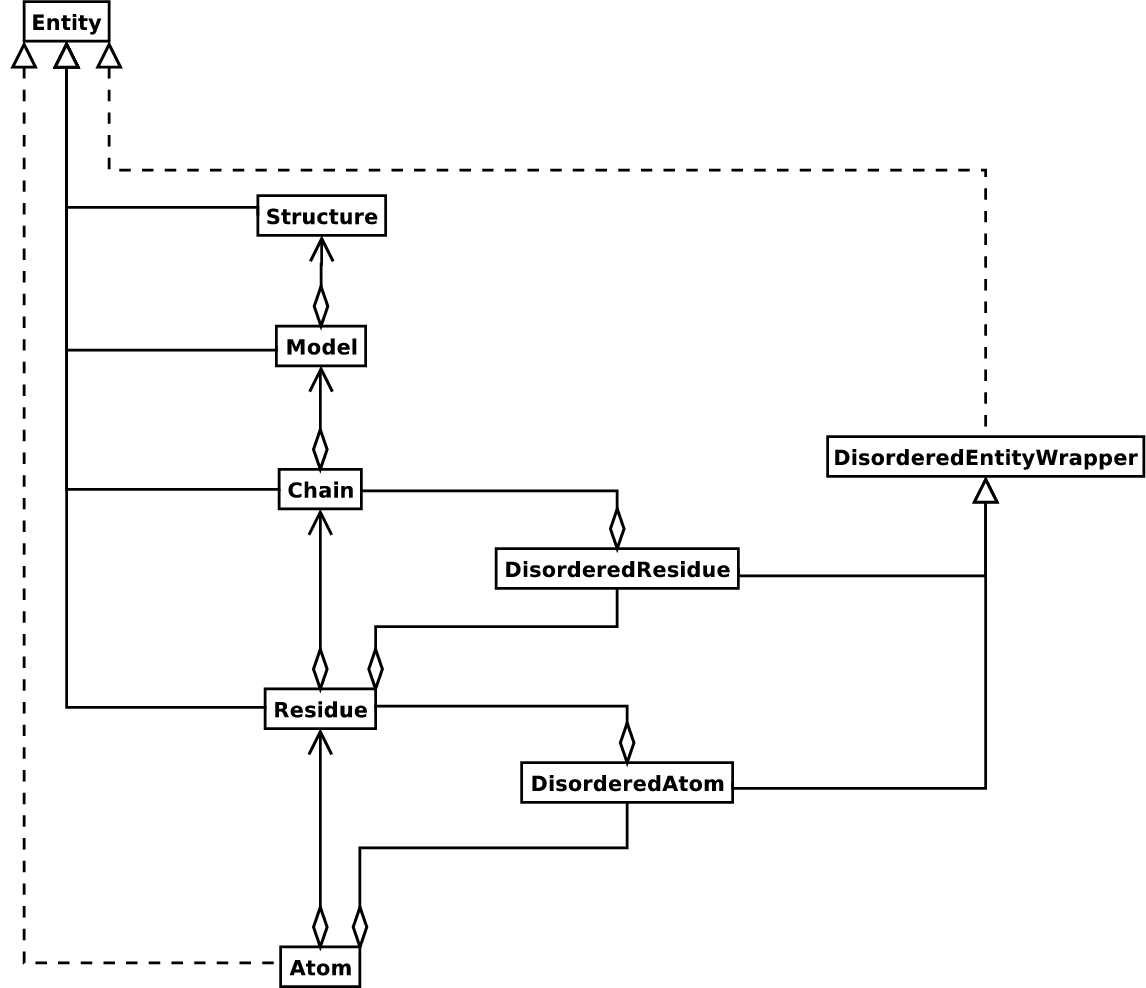
\includegraphics{smcra.png}

图11.1:用来表示大分子结构的 \code{Structure} 类的SMCRA体系的UML图。带方块的实线表示集合,带箭头的实线表示引用,带三角形的实线表示继承,带三角形的虚线表示接口实现。


\bigskip\hrule{}\bigskip


结构,模型,链,残基都是实体基类的子类。原子类仅仅(部分)实现了实体接口(因为原子类没有子类)。

对于每个实体子类,你可以用该子类的一个唯一标识符作为键来提取子类(比如,可以用原子名称作为键从残基对象中提取一个原子对象;用链的标识符作为键从域对象中提取链)。

紊乱原子和残基用DisorderedAtom和DisorderedResidue类来表示,二者都是DisorderedEntityWrapper基类的子类。它们隐藏了紊乱的复杂性,表现得与原子和残基对象无二。

一般地,一个实体子类(即原子,残基,链,模型)能通过标识符作为键来从父类(分别为残基,链,模型,结构)中提取。
\DUspan{operator}{}\DUspan{name}{}\DUspan{operator}{}\DUspan{name}{}\DUspan{punctuation}{}\DUspan{name}{}\DUspan{punctuation}{}
\begin{Verbatim}[commandchars=\\\{\}]
\PYG{g+gp}{\PYGZgt{}\PYGZgt{}\PYGZgt{} }\PYG{n}{child\PYGZus{}entity} \PYG{o}{=} \PYG{n}{parent\PYGZus{}entity}\PYG{p}{[}\PYG{n}{child\PYGZus{}id}\PYG{p}{]}
\end{Verbatim}

你可以从一个父实体对象获得所有子实体的列表。需要注意的是,这个列表以一种特定的方式排列(例如根据在模型对象中链对象的链标识符来排序)。
\DUspan{operator}{}\DUspan{name}{}\DUspan{operator}{}\DUspan{name}{}\DUspan{operator}{}\DUspan{name}{}\DUspan{punctuation}{}
\begin{Verbatim}[commandchars=\\\{\}]
\PYG{g+gp}{\PYGZgt{}\PYGZgt{}\PYGZgt{} }\PYG{n}{child\PYGZus{}list} \PYG{o}{=} \PYG{n}{parent\PYGZus{}entity}\PYG{o}{.}\PYG{n}{get\PYGZus{}list}\PYG{p}{(}\PYG{p}{)}
\end{Verbatim}

你也可以从子类得到父类:
\DUspan{operator}{}\DUspan{name}{}\DUspan{operator}{}\DUspan{name}{}\DUspan{operator}{}\DUspan{name}{}\DUspan{punctuation}{}
\begin{Verbatim}[commandchars=\\\{\}]
\PYG{g+gp}{\PYGZgt{}\PYGZgt{}\PYGZgt{} }\PYG{n}{parent\PYGZus{}entity} \PYG{o}{=} \PYG{n}{child\PYGZus{}entity}\PYG{o}{.}\PYG{n}{get\PYGZus{}parent}\PYG{p}{(}\PYG{p}{)}
\end{Verbatim}

在SMCRA的所有层次水平,你还可以提取一个 \emph{完整id} 。完整id是包含所有从顶层对象(结构)到当前对象的id的一个元组。一个残基对象的完整id可以这么得到:
\DUspan{operator}{}\DUspan{name}{}\DUspan{operator}{}\DUspan{name}{}\DUspan{operator}{}\DUspan{name}{}\DUspan{punctuation}{}\DUspan{operator}{}\DUspan{keyword}{}\DUspan{name}{}\DUspan{punctuation}{}\DUspan{literal,string}{}\DUspan{punctuation}{}\DUspan{literal,number,integer}{}\DUspan{punctuation}{}\DUspan{literal,string}{}\DUspan{punctuation}{}\DUspan{punctuation}{}\DUspan{literal,string}{}\DUspan{punctuation}{}\DUspan{literal,number,integer}{}\DUspan{punctuation}{}\DUspan{literal,string}{}\DUspan{punctuation}{}
\begin{Verbatim}[commandchars=\\\{\}]
\PYG{g+gp}{\PYGZgt{}\PYGZgt{}\PYGZgt{} }\PYG{n}{full\PYGZus{}id} \PYG{o}{=} \PYG{n}{residue}\PYG{o}{.}\PYG{n}{get\PYGZus{}full\PYGZus{}id}\PYG{p}{(}\PYG{p}{)}
\PYG{g+gp}{\PYGZgt{}\PYGZgt{}\PYGZgt{} }\PYG{k}{print} \PYG{n}{full\PYGZus{}id}
\PYG{g+go}{(\PYGZdq{}1abc\PYGZdq{}, 0, \PYGZdq{}A\PYGZdq{}, (\PYGZdq{}\PYGZdq{}, 10, \PYGZdq{}A\PYGZdq{}))}
\end{Verbatim}

这对应于:
\begin{itemize}
\item {} 
id为''1abc''的结构

\item {} 
id为0的模型

\item {} 
id为''A''的链

\item {} 
id为('' '', 10, ``A'')的残基

\end{itemize}

这个残基id表示该残基不是异质残基(也不是水分子),因为其异质值为空;而序列标识符为10,插入码为''A''。

要得到实体的id,用 \code{get\_id} 方法即可:
\DUspan{operator}{}\DUspan{name}{}\DUspan{operator}{}\DUspan{name}{}\DUspan{punctuation}{}
\begin{Verbatim}[commandchars=\\\{\}]
\PYG{g+gp}{\PYGZgt{}\PYGZgt{}\PYGZgt{} }\PYG{n}{entity}\PYG{o}{.}\PYG{n}{get\PYGZus{}id}\PYG{p}{(}\PYG{p}{)}
\end{Verbatim}

可以用 \code{has\_id} 方法来检查这个实体是否有子类具有给定id:
\DUspan{operator}{}\DUspan{name}{}\DUspan{operator}{}\DUspan{name}{}\DUspan{punctuation}{}\DUspan{name}{}\DUspan{punctuation}{}
\begin{Verbatim}[commandchars=\\\{\}]
\PYG{g+gp}{\PYGZgt{}\PYGZgt{}\PYGZgt{} }\PYG{n}{entity}\PYG{o}{.}\PYG{n}{has\PYGZus{}id}\PYG{p}{(}\PYG{n}{entity\PYGZus{}id}\PYG{p}{)}
\end{Verbatim}

实体的长度等于其子类的个数:
\DUspan{operator}{}\DUspan{name}{}\DUspan{operator}{}\DUspan{name,builtin}{}\DUspan{punctuation}{}\DUspan{name}{}\DUspan{punctuation}{}
\begin{Verbatim}[commandchars=\\\{\}]
\PYG{g+gp}{\PYGZgt{}\PYGZgt{}\PYGZgt{} }\PYG{n}{nr\PYGZus{}children} \PYG{o}{=} \PYG{n+nb}{len}\PYG{p}{(}\PYG{n}{entity}\PYG{p}{)}
\end{Verbatim}

对于从父实体得到的子实体,可以删除,重命名,添加等等,但这并不包含任何完整性检查(比如,有可能添加两个相同id的残基到同一条链上)。这就真的需要包含完整性检查的装饰类(Decorator)来完成了,但是如果你想使用原始接口的话可以查看源代码(Entity.py)。


\subsection{11.2.1  结构}
\label{chr11:id4}
结构对象是层次中的最高层。其id是用户指定的一个字符串。结构包含一系列子模型。大部分晶体结构(但不是全部)含有一个单一模型,但是NMR结构通常由若干模型构成。晶体结构中大部分子的乱序也能导致多个模型。


\subsection{11.2.2  模型}
\label{chr11:id5}
结构域对象的id是一个整数,源自该模型在所解析文件中的位置(自动从0开始)。晶体结构通常只有一个模型(id为0),而NMR文件通常含有多个模型。然而许多PDB解析器都假定只有一个结构域, \code{Bio.PDB} 中的 \code{Structure} 类就设计成能轻松处理含有不止一个模型的PDB文件。

举个例子,从一个结构对象中获取其第一个模型:
\DUspan{operator}{}\DUspan{name}{}\DUspan{operator}{}\DUspan{name}{}\DUspan{punctuation}{}\DUspan{literal,number,integer}{}\DUspan{punctuation}{}
\begin{Verbatim}[commandchars=\\\{\}]
\PYG{g+gp}{\PYGZgt{}\PYGZgt{}\PYGZgt{} }\PYG{n}{first\PYGZus{}model} \PYG{o}{=} \PYG{n}{structure}\PYG{p}{[}\PYG{l+m+mi}{0}\PYG{p}{]}
\end{Verbatim}

模型对象存储着子链的列表。


\subsection{11.2.3  链}
\label{chr11:id6}
链对象的id来自PDB/mmCIF文件中的链标识符,是个单字符(通常是一个字母)。模型中的每个链都具有唯一的id。例如,从一个模型对象中取出标识符为“A”的链对象:
\DUspan{operator}{}\DUspan{name}{}\DUspan{operator}{}\DUspan{name}{}\DUspan{punctuation}{}\DUspan{literal,string}{}\DUspan{punctuation}{}
\begin{Verbatim}[commandchars=\\\{\}]
\PYG{g+gp}{\PYGZgt{}\PYGZgt{}\PYGZgt{} }\PYG{n}{chain\PYGZus{}A} \PYG{o}{=} \PYG{n}{model}\PYG{p}{[}\PYG{l+s}{\PYGZdq{}}\PYG{l+s}{A}\PYG{l+s}{\PYGZdq{}}\PYG{p}{]}
\end{Verbatim}

链对象储存着残基对象的列表。


\subsection{11.2.4  残基}
\label{chr11:id7}
一个残基id是一个三元组:
\begin{itemize}
\item {} 
\textbf{异质域} (hetfield),即:
\begin{itemize}
\item {} 
\code{'W'} 代表水分子

\item {} 
\code{'H\_'} 后面紧跟残基名称,代表其它异质残基(例如 \code{'H\_GLC'} 表示一个葡萄糖分子)

\item {} 
空值表示标准的氨基酸和核酸

\end{itemize}

采用这种体制的理由在 {\hyperref[chr11:sec-hetero-problems]{\emph{11.4.1}}} 部分有叙述。

\item {} 
\textbf{序列标识符} (resseq),一个描述该残基在链上的位置的整数(如100);

\item {} 
\textbf{插入码} (icode),一个字符串,如“A”。插入码有时用来保存某种特定的、想要的残基编号体制。一个Ser 80的插入突变(比如在Thr 80和Asn 81残基间插入)可能具有如下序列标识符和插入码:Thr 80 A, Ser 80 B, Asn 81。这样一来,残基编号体制保持与野生型结构一致。

\end{itemize}

因此,上述的葡萄酸残基id就是 \code{(’H\_GLC’, 100, ’A’)} 。如果异质标签和插入码为空,那么可以只使用序列标识符:
\DUspan{comment}{}\DUspan{operator}{}\DUspan{name}{}\DUspan{operator}{}\DUspan{name}{}\DUspan{punctuation}{}\DUspan{literal,string}{}\DUspan{punctuation}{}\DUspan{literal,number,integer}{}\DUspan{punctuation}{}\DUspan{literal,string}{}\DUspan{punctuation}{}\DUspan{comment}{}\DUspan{operator}{}\DUspan{name}{}\DUspan{operator}{}\DUspan{name}{}\DUspan{punctuation}{}\DUspan{literal,number,integer}{}\DUspan{punctuation}{}
\begin{Verbatim}[commandchars=\\\{\}]
\# Full id
\textgreater{}\textgreater{}\textgreater{} residue=chain[(' ', 100, ' ')]
\# Shortcut id
\textgreater{}\textgreater{}\textgreater{} residue=chain[100]
\end{Verbatim}

异质标签的起因是许许多多的PDB文件使用相同的序列标识符表示一个氨基酸和一个异质残基或一个水分子,这会产生一个很明显的问题,如果不使用异质标签的话。

毫不奇怪,一个残基对象存储着一个子原子集,它还包含一个表示残基名称的字符串(如 “ASN”)和残基的片段标识符(这对X-PLOR的用户来说很熟悉,但是在SMCRA数据结构的构建中没用到)。

让我们来看一些例子。插入码为空的Asn 10具有残基id \code{(’ ’, 10, ’ ’)} ;Water 10,残基id \code{(’W’, 10, ’ ’)};一个序列标识符为10的葡萄糖分子(名称为GLC的异质残基),残基id为 \code{(’H\_GLC’, 10, ’ ’)} 。在这种情况下,三个残基(具有相同插入码和序列标识符)可以位于同一条链上,因为它们的残基id是不同的。

大多数情况下,hetflag和插入码均为空,如 \code{(’ ’, 10, ’ ’)} 。在这些情况下,序列标识符可以用作完整id的快捷方式:
\DUspan{comment}{}\DUspan{operator}{}\DUspan{name}{}\DUspan{operator}{}\DUspan{name}{}\DUspan{punctuation}{}\DUspan{literal,string}{}\DUspan{punctuation}{}\DUspan{literal,number,integer}{}\DUspan{punctuation}{}\DUspan{literal,string}{}\DUspan{punctuation}{}\DUspan{comment}{}\DUspan{operator}{}\DUspan{name}{}\DUspan{operator}{}\DUspan{name}{}\DUspan{punctuation}{}\DUspan{literal,number,integer}{}\DUspan{punctuation}{}
\begin{Verbatim}[commandchars=\\\{\}]
\# use full id
\textgreater{}\textgreater{}\textgreater{} res10 = chain[(' ', 10, ' ')]
\# use shortcut
\textgreater{}\textgreater{}\textgreater{} res10 = chain[10]
\end{Verbatim}

一个链对象中每个残基对象都应该具有唯一的id。但是对含紊乱原子的残基,要以一种特殊的方式来处理,详见 {\hyperref[chr11:sec-point-mutations]{\emph{11.3.3}}} 。

一个残基对象还有大量其它方法:
\DUspan{operator}{}\DUspan{name}{}\DUspan{operator}{}\DUspan{name}{}\DUspan{punctuation}{}\DUspan{comment}{}\DUspan{operator}{}\DUspan{name}{}\DUspan{operator}{}\DUspan{name}{}\DUspan{punctuation}{}\DUspan{comment}{}\DUspan{operator}{}\DUspan{name}{}\DUspan{operator}{}\DUspan{name}{}\DUspan{punctuation}{}\DUspan{comment}{}\DUspan{operator}{}\DUspan{name}{}\DUspan{operator}{}\DUspan{name}{}\DUspan{punctuation}{}\DUspan{name}{}\DUspan{punctuation}{}\DUspan{comment}{}
\begin{Verbatim}[commandchars=\\\{\}]
\PYG{g+gp}{\PYGZgt{}\PYGZgt{}\PYGZgt{} }\PYG{n}{residue}\PYG{o}{.}\PYG{n}{get\PYGZus{}resname}\PYG{p}{(}\PYG{p}{)}       \PYG{c}{\PYGZsh{} returns the residue name, e.g. \PYGZdq{}ASN\PYGZdq{}}
\PYG{g+gp}{\PYGZgt{}\PYGZgt{}\PYGZgt{} }\PYG{n}{residue}\PYG{o}{.}\PYG{n}{is\PYGZus{}disordered}\PYG{p}{(}\PYG{p}{)}     \PYG{c}{\PYGZsh{} returns 1 if the residue has disordered atoms}
\PYG{g+gp}{\PYGZgt{}\PYGZgt{}\PYGZgt{} }\PYG{n}{residue}\PYG{o}{.}\PYG{n}{get\PYGZus{}segid}\PYG{p}{(}\PYG{p}{)}         \PYG{c}{\PYGZsh{} returns the SEGID, e.g. \PYGZdq{}CHN1\PYGZdq{}}
\PYG{g+gp}{\PYGZgt{}\PYGZgt{}\PYGZgt{} }\PYG{n}{residue}\PYG{o}{.}\PYG{n}{has\PYGZus{}id}\PYG{p}{(}\PYG{n}{name}\PYG{p}{)}        \PYG{c}{\PYGZsh{} test if a residue has a certain atom}
\end{Verbatim}

你可以用 \code{is\_aa(residue)} 来检验一个残基对象是否为氨基酸。


\subsection{11.2.5  原子}
\label{chr11:id8}
原子对象储存着所有与原子有关的数据,它没有子类。原子的id就是它的名称(如,“OG”代表Ser残基的侧链氧原子)。在残基中原子id必需是唯一的。此外,对于紊乱原子会产生异常,见 {\hyperref[chr11:sec-disordered-atoms]{\emph{11.3.2}}} 小节的描述。

原子id就是原子名称(如 \code{’CA’} )。在实践中,原子名称是从PDB文件中原子名称去除所有空格而创建的。

但是在PDB文件中,空格可以是原子名称的一部分。通常,钙原子称为 \code{’CA..’} 是为了和C\(\alpha\)原子(叫做 \code{’.CA.’} )区分开。在这种情况下,如果去掉空格就会产生问题(如统一个残基中的两个原子都叫做 \code{’CA’} ),所以保留空格。

在PDB文件中,一个原子名字由4个字符组成,通常头尾皆为空格。为了方便使用,空格通常可以去掉(在PDB文件中氨基酸的C\(\alpha\)原子标记为“.CA.”,点表示空格)。为了生成原子名称(然后是原子id),空格删掉了,除非会在一个残基中造成名字冲突(如两个原子对象有相同的名称和id)。对于后面这种情况,会尝试让原子名称包含空格。这种情况可能会发生在,比如残基包含名称为“.CA.”和“CA..”的原子,尽管这不怎么可能。

所存储的原子数据包括原子名称,原子坐标(如果有的话还包括标准差),B因子(包括各向异性B因子和可能存在的标准差),altloc标识符和完整的、包括空格的原子名称。较少用到的项如原子序号和原子电荷(有时在PDB文件中规定)也就没有存储。

为了处理原子坐标,可以用 \code{’Atom’} 对象的 \code{transform} 方法。用 \code{set\_coord} 方法可以直接设定原子坐标。

一个Atom对象还有如下其它方法:
\DUspan{operator}{}\DUspan{name}{}\DUspan{operator}{}\DUspan{name}{}\DUspan{punctuation}{}\DUspan{comment}{}\DUspan{operator}{}\DUspan{name}{}\DUspan{operator}{}\DUspan{name}{}\DUspan{punctuation}{}\DUspan{comment}{}\DUspan{operator}{}\DUspan{name}{}\DUspan{operator}{}\DUspan{name}{}\DUspan{punctuation}{}\DUspan{comment}{}\DUspan{operator}{}\DUspan{name}{}\DUspan{operator}{}\DUspan{name}{}\DUspan{punctuation}{}\DUspan{comment}{}\DUspan{operator}{}\DUspan{name}{}\DUspan{operator}{}\DUspan{name}{}\DUspan{punctuation}{}\DUspan{comment}{}\DUspan{operator}{}\DUspan{name}{}\DUspan{operator}{}\DUspan{name}{}\DUspan{punctuation}{}\DUspan{comment}{}\DUspan{operator}{}\DUspan{name}{}\DUspan{operator}{}\DUspan{name}{}\DUspan{punctuation}{}\DUspan{comment}{}\DUspan{operator}{}\DUspan{name}{}\DUspan{operator}{}\DUspan{name}{}\DUspan{punctuation}{}\DUspan{comment}{}\DUspan{operator}{}\DUspan{name}{}\DUspan{operator}{}\DUspan{name}{}\DUspan{punctuation}{}\DUspan{comment}{}\DUspan{operator}{}\DUspan{name}{}\DUspan{operator}{}\DUspan{name}{}\DUspan{punctuation}{}\DUspan{comment}{}\DUspan{operator}{}\DUspan{name}{}\DUspan{operator}{}\DUspan{name}{}\DUspan{punctuation}{}\DUspan{comment}{}
\begin{Verbatim}[commandchars=\\\{\}]
\PYG{g+gp}{\PYGZgt{}\PYGZgt{}\PYGZgt{} }\PYG{n}{a}\PYG{o}{.}\PYG{n}{get\PYGZus{}name}\PYG{p}{(}\PYG{p}{)}       \PYG{c}{\PYGZsh{} atom name (spaces stripped, e.g. \PYGZdq{}CA\PYGZdq{})}
\PYG{g+gp}{\PYGZgt{}\PYGZgt{}\PYGZgt{} }\PYG{n}{a}\PYG{o}{.}\PYG{n}{get\PYGZus{}id}\PYG{p}{(}\PYG{p}{)}         \PYG{c}{\PYGZsh{} id (equals atom name)}
\PYG{g+gp}{\PYGZgt{}\PYGZgt{}\PYGZgt{} }\PYG{n}{a}\PYG{o}{.}\PYG{n}{get\PYGZus{}coord}\PYG{p}{(}\PYG{p}{)}      \PYG{c}{\PYGZsh{} atomic coordinates}
\PYG{g+gp}{\PYGZgt{}\PYGZgt{}\PYGZgt{} }\PYG{n}{a}\PYG{o}{.}\PYG{n}{get\PYGZus{}vector}\PYG{p}{(}\PYG{p}{)}     \PYG{c}{\PYGZsh{} atomic coordinates as Vector object}
\PYG{g+gp}{\PYGZgt{}\PYGZgt{}\PYGZgt{} }\PYG{n}{a}\PYG{o}{.}\PYG{n}{get\PYGZus{}bfactor}\PYG{p}{(}\PYG{p}{)}    \PYG{c}{\PYGZsh{} isotropic B factor}
\PYG{g+gp}{\PYGZgt{}\PYGZgt{}\PYGZgt{} }\PYG{n}{a}\PYG{o}{.}\PYG{n}{get\PYGZus{}occupancy}\PYG{p}{(}\PYG{p}{)}  \PYG{c}{\PYGZsh{} occupancy}
\PYG{g+gp}{\PYGZgt{}\PYGZgt{}\PYGZgt{} }\PYG{n}{a}\PYG{o}{.}\PYG{n}{get\PYGZus{}altloc}\PYG{p}{(}\PYG{p}{)}     \PYG{c}{\PYGZsh{} alternative location specifier}
\PYG{g+gp}{\PYGZgt{}\PYGZgt{}\PYGZgt{} }\PYG{n}{a}\PYG{o}{.}\PYG{n}{get\PYGZus{}sigatm}\PYG{p}{(}\PYG{p}{)}     \PYG{c}{\PYGZsh{} standard deviation of atomic parameters}
\PYG{g+gp}{\PYGZgt{}\PYGZgt{}\PYGZgt{} }\PYG{n}{a}\PYG{o}{.}\PYG{n}{get\PYGZus{}siguij}\PYG{p}{(}\PYG{p}{)}     \PYG{c}{\PYGZsh{} standard deviation of anisotropic B factor}
\PYG{g+gp}{\PYGZgt{}\PYGZgt{}\PYGZgt{} }\PYG{n}{a}\PYG{o}{.}\PYG{n}{get\PYGZus{}anisou}\PYG{p}{(}\PYG{p}{)}     \PYG{c}{\PYGZsh{} anisotropic B factor}
\PYG{g+gp}{\PYGZgt{}\PYGZgt{}\PYGZgt{} }\PYG{n}{a}\PYG{o}{.}\PYG{n}{get\PYGZus{}fullname}\PYG{p}{(}\PYG{p}{)}   \PYG{c}{\PYGZsh{} atom name (with spaces, e.g. \PYGZdq{}.CA.\PYGZdq{})}
\end{Verbatim}

siguij,各向异性B因子和sigatm Numpy阵列可以用来表示原子坐标。

\code{get\_vector} 方法会返回一个代表 \code{Atom}  对象坐标的 \code{Vector} 对象,可以对原子坐标进行向量运算。 \code{Vector} 实现了完整的三维向量运算、矩阵乘法(包括左乘和右乘)和一些高级的、与旋转相关的操作。

举个Bio.PDB的 \code{Vector} 模块功能的例子,假设你要查找Gly残基的C\(\beta\)原子的位置,如果存在的话。将Gly残基的N原子沿C\(\alpha\)-C化学键旋转-120度,能大致将其放在一个真正的C\(\beta\)原子的位置上。怎么做呢?就是下面这样使用 \code{Vector} 模块中的{}`{}`rotaxis{}`{}` 方法(能用来构造一个绕特定坐标轴的旋转):
\DUspan{comment}{}\DUspan{operator}{}\DUspan{name}{}\DUspan{operator}{}\DUspan{name}{}\DUspan{punctuation}{}\DUspan{literal,string}{}\DUspan{punctuation}{}\DUspan{operator}{}\DUspan{name}{}\DUspan{punctuation}{}\DUspan{operator}{}\DUspan{name}{}\DUspan{operator}{}\DUspan{name}{}\DUspan{punctuation}{}\DUspan{literal,string}{}\DUspan{punctuation}{}\DUspan{operator}{}\DUspan{name}{}\DUspan{punctuation}{}\DUspan{operator}{}\DUspan{name}{}\DUspan{operator}{}\DUspan{name}{}\DUspan{punctuation}{}\DUspan{literal,string}{}\DUspan{punctuation}{}\DUspan{operator}{}\DUspan{name}{}\DUspan{punctuation}{}\DUspan{comment}{}\DUspan{operator}{}\DUspan{name}{}\DUspan{operator}{}\DUspan{name}{}\DUspan{operator}{}\DUspan{name}{}\DUspan{operator}{}\DUspan{name}{}\DUspan{operator}{}\DUspan{name}{}\DUspan{operator}{}\DUspan{name}{}\DUspan{comment}{}\DUspan{comment}{}\DUspan{operator}{}\DUspan{name}{}\DUspan{operator}{}\DUspan{name}{}\DUspan{punctuation}{}\DUspan{operator}{}\DUspan{name}{}\DUspan{operator}{}\DUspan{literal,number,float}{}\DUspan{operator}{}\DUspan{literal,number,float}{}\DUspan{punctuation}{}\DUspan{name}{}\DUspan{punctuation}{}\DUspan{comment}{}\DUspan{operator}{}\DUspan{name}{}\DUspan{operator}{}\DUspan{name}{}\DUspan{operator}{}\DUspan{name}{}\DUspan{punctuation}{}\DUspan{name}{}\DUspan{punctuation}{}\DUspan{comment}{}\DUspan{operator}{}\DUspan{name}{}\DUspan{operator}{}\DUspan{name}{}\DUspan{operator}{}\DUspan{name}{}
\begin{Verbatim}[commandchars=\\\{\}]
\# get atom coordinates as vectors
\textgreater{}\textgreater{}\textgreater{} n = residue['N'].get\_vector()
\textgreater{}\textgreater{}\textgreater{} c = residue['C'].get\_vector()
\textgreater{}\textgreater{}\textgreater{} ca = residue['CA'].get\_vector()
\# center at origin
\textgreater{}\textgreater{}\textgreater{} n = n - ca
\textgreater{}\textgreater{}\textgreater{} c = c - ca
\# find rotation matrix that rotates n
\# -120 degrees along the ca-c vector
\textgreater{}\textgreater{}\textgreater{} rot = rotaxis(-pi * 120.0/180.0, c)
\# apply rotation to ca-n vector
\textgreater{}\textgreater{}\textgreater{} cb\_at\_origin = n.left\_multiply(rot)
\# put on top of ca atom
\textgreater{}\textgreater{}\textgreater{} cb = cb\_at\_origin+ca
\end{Verbatim}

这个例子展示了在原子数据上能进行一些相当不平凡的向量运算,这些运算会很有用。除了所有常用向量运算(叉积(用 \code{*}\code{*} ),点积(用 \code{*} ),角度, 取范数等)和上述提到的 \code{rotaxis} 函数,\code{Vector} 模块还有方法能旋转( \code{rotmat} )或反射( \code{refmat} )一个向量到另外一个向量上。


\subsection{11.2.6  从结构中提取指定的 \texttt{Atom/Residue/Chain/Model}}
\label{chr11:atom-residue-chain-model}
举些例子如下:
\DUspan{operator}{}\DUspan{name}{}\DUspan{operator}{}\DUspan{name}{}\DUspan{punctuation}{}\DUspan{literal,number,integer}{}\DUspan{punctuation}{}\DUspan{operator}{}\DUspan{name}{}\DUspan{operator}{}\DUspan{name}{}\DUspan{punctuation}{}\DUspan{literal,string}{}\DUspan{punctuation}{}\DUspan{operator}{}\DUspan{name}{}\DUspan{operator}{}\DUspan{name}{}\DUspan{punctuation}{}\DUspan{literal,number,integer}{}\DUspan{punctuation}{}\DUspan{operator}{}\DUspan{name}{}\DUspan{operator}{}\DUspan{name}{}\DUspan{punctuation}{}\DUspan{literal,string}{}\DUspan{punctuation}{}
\begin{Verbatim}[commandchars=\\\{\}]
\PYG{g+gp}{\PYGZgt{}\PYGZgt{}\PYGZgt{} }\PYG{n}{model} \PYG{o}{=} \PYG{n}{structure}\PYG{p}{[}\PYG{l+m+mi}{0}\PYG{p}{]}
\PYG{g+gp}{\PYGZgt{}\PYGZgt{}\PYGZgt{} }\PYG{n}{chain} \PYG{o}{=} \PYG{n}{model}\PYG{p}{[}\PYG{l+s}{\PYGZsq{}}\PYG{l+s}{A}\PYG{l+s}{\PYGZsq{}}\PYG{p}{]}
\PYG{g+gp}{\PYGZgt{}\PYGZgt{}\PYGZgt{} }\PYG{n}{residue} \PYG{o}{=} \PYG{n}{chain}\PYG{p}{[}\PYG{l+m+mi}{100}\PYG{p}{]}
\PYG{g+gp}{\PYGZgt{}\PYGZgt{}\PYGZgt{} }\PYG{n}{atom} \PYG{o}{=} \PYG{n}{residue}\PYG{p}{[}\PYG{l+s}{\PYGZsq{}}\PYG{l+s}{CA}\PYG{l+s}{\PYGZsq{}}\PYG{p}{]}
\end{Verbatim}

还可以用一个快捷方式:
\DUspan{operator}{}\DUspan{name}{}\DUspan{operator}{}\DUspan{name}{}\DUspan{punctuation}{}\DUspan{literal,number,integer}{}\DUspan{punctuation}{}\DUspan{literal,string}{}\DUspan{punctuation}{}\DUspan{literal,number,integer}{}\DUspan{punctuation}{}\DUspan{literal,string}{}\DUspan{punctuation}{}
\begin{Verbatim}[commandchars=\\\{\}]
\PYG{g+gp}{\PYGZgt{}\PYGZgt{}\PYGZgt{} }\PYG{n}{atom} \PYG{o}{=} \PYG{n}{structure}\PYG{p}{[}\PYG{l+m+mi}{0}\PYG{p}{]}\PYG{p}{[}\PYG{l+s}{\PYGZsq{}}\PYG{l+s}{A}\PYG{l+s}{\PYGZsq{}}\PYG{p}{]}\PYG{p}{[}\PYG{l+m+mi}{100}\PYG{p}{]}\PYG{p}{[}\PYG{l+s}{\PYGZsq{}}\PYG{l+s}{CA}\PYG{l+s}{\PYGZsq{}}\PYG{p}{]}
\end{Verbatim}


\section{11.3  紊乱}
\label{chr11:id9}
Bio.PDB能够处理紊乱原子和点突变(比如Gly和Ala残基在相同位置上)。


\subsection{11.3.1  一般性方法}
\label{chr11:id10}
紊乱可以从两个角度来解决:原子和残基的角度。一般来说,我们尝试压缩所有由紊乱引起的复杂性。如果你仅仅想遍历所有C\(\alpha\)原子,那么你不必在意一些具有紊乱侧链的残基。另一方面,应该考虑在数据结构中完整地表示紊乱性。因此,紊乱原子或残基存储在特定的对象中,这些对象表现得就像毫无紊乱。这可以通过表示紊乱原子或残基的子集来完成。至于挑选哪个子集(例如使用Ser残基的哪两个紊乱OG侧链原子位置),由用户来决定。


\subsection{11.3.2  紊乱原子}
\label{chr11:id11}\label{chr11:sec-disordered-atoms}
紊乱原子可以用普通的 \code{Atom} 对象来表示,但是所有表示相同物理原子的 \code{Atom} 对象都存储在一个 \code{DisorderedAtom} 对象中(见图. {\hyperref[chr11:fig-smcra]{\emph{11.1}}} )。 \code{DisorderedAtom} 对象中每个 \code{Atom} 对象都能用它的altloc标识符来唯一地索引。 \code{DisorderedAtom} 对象将所有未捕获方法的调用发送给选定的Atom对象,缺省对象是代表最高使用率的原子的那个。当然用户可以使用其altloc标识符来更改选定的 \code{Atom} 对象。以这种方式,原子紊乱就正确地表示出来而没有很多额外的复杂性。换言之,如果你对原子紊乱不感兴趣,你也不会被它困扰。

每个紊乱原子都有一个特征性的altloc标识符。你可以设定:一个 \code{DisorderedAtom} 对象表现得像与一个指定的altloc标识符相关的 \code{Atom} 对象:
\DUspan{operator}{}\DUspan{name}{}\DUspan{operator}{}\DUspan{name}{}\DUspan{punctuation}{}\DUspan{literal,string}{}\DUspan{punctuation}{}\DUspan{comment}{}\DUspan{operator}{}\DUspan{keyword}{}\DUspan{name}{}\DUspan{operator}{}\DUspan{name}{}\DUspan{punctuation}{}\DUspan{literal,string}{}\DUspan{operator}{}\DUspan{name}{}\DUspan{operator}{}\DUspan{name}{}\DUspan{punctuation}{}\DUspan{literal,string}{}\DUspan{punctuation}{}\DUspan{comment}{}\DUspan{operator}{}\DUspan{keyword}{}\DUspan{name}{}\DUspan{operator}{}\DUspan{name}{}\DUspan{punctuation}{}\DUspan{literal,string}{}
\begin{Verbatim}[commandchars=\\\{\}]
\PYG{g+gp}{\PYGZgt{}\PYGZgt{}\PYGZgt{} }\PYG{n}{atom}\PYG{o}{.}\PYG{n}{disordered\PYGZus{}select}\PYG{p}{(}\PYG{l+s}{\PYGZsq{}}\PYG{l+s}{A}\PYG{l+s}{\PYGZsq{}}\PYG{p}{)} \PYG{c}{\PYGZsh{} select altloc A atom}
\PYG{g+gp}{\PYGZgt{}\PYGZgt{}\PYGZgt{} }\PYG{k}{print} \PYG{n}{atom}\PYG{o}{.}\PYG{n}{get\PYGZus{}altloc}\PYG{p}{(}\PYG{p}{)}
\PYG{g+go}{\PYGZdq{}A\PYGZdq{}}
\PYG{g+gp}{\PYGZgt{}\PYGZgt{}\PYGZgt{} }\PYG{n}{atom}\PYG{o}{.}\PYG{n}{disordered\PYGZus{}select}\PYG{p}{(}\PYG{l+s}{\PYGZsq{}}\PYG{l+s}{B}\PYG{l+s}{\PYGZsq{}}\PYG{p}{)} \PYG{c}{\PYGZsh{} select altloc B atom}
\PYG{g+gp}{\PYGZgt{}\PYGZgt{}\PYGZgt{} }\PYG{k}{print} \PYG{n}{atom}\PYG{o}{.}\PYG{n}{get\PYGZus{}altloc}\PYG{p}{(}\PYG{p}{)}
\PYG{g+go}{\PYGZdq{}B\PYGZdq{}}
\end{Verbatim}


\subsection{11.3.3  紊乱残基}
\label{chr11:id12}\label{chr11:sec-point-mutations}

\subsubsection{普通例子}
\label{chr11:id13}
最常见的例子是一个残基包含一个或多个紊乱原子。这显然可以通过用DisorderedAtom对象表示这些紊乱原子来解决,并将DisorderedAtom对象存储在一个Residue对象中,就像正常的Atom对象那样。通过将所有未捕获方法调用发送给其中一个Atom对象(被选定的Atom对象),DisorderedAtom对象表现完全像一个正常的原子对象(事实上这个原子有最高的使用率)。


\subsubsection{点突变}
\label{chr11:id14}
一个特殊的例子就是当紊乱是由点突变导致的时候,也就是说,在晶体结构中出现一条多肽的两或多个点突变。关于这一点,可以在PDB结构1EN2中找到一个例子。

既然这些残基属于不同的残基类型(举例说Ser 60 和Cys 60),那么它们不应该像通常情况一样存储在一个单一 \code{Residue} 对象中。这种情况下每个残基用一个 \code{Residue} 对象来表示,两种 \code{Residue} 对象都保存在一个单一 \code{DisorderedResidue} 对象中(见图. {\hyperref[chr11:fig-smcra]{\emph{11.1}}} )。

\code{DisorderedResidue} 对象将所有未捕获方法发送给选定的 \code{Residue} 对象(默认是所添加的最后一个 \code{Residue} 对象),因此表现得像一个正常的残基。在 \code{DisorderedResidue} 中每个 \code{Residue} 对象可通过残基名称来唯一标识。在上述例子中,残基Ser 60在 \code{DisorderedResidue} 对象中的id为“SER”,而残基Cys 60则是“CYS”。用户可以通过这个id选择在 \code{DisorderedResidue} 中的有效 \code{Residue} 对象。

例子:假设一个链在位置10有一个由Ser和Cys残基构成的点突变。确信这个链的残基10表现为Cys残基。
\DUspan{operator}{}\DUspan{name}{}\DUspan{operator}{}\DUspan{name}{}\DUspan{punctuation}{}\DUspan{literal,number,integer}{}\DUspan{punctuation}{}\DUspan{operator}{}\DUspan{name}{}\DUspan{operator}{}\DUspan{name}{}\DUspan{punctuation}{}\DUspan{literal,string}{}\DUspan{punctuation}{}
\begin{Verbatim}[commandchars=\\\{\}]
\PYG{g+gp}{\PYGZgt{}\PYGZgt{}\PYGZgt{} }\PYG{n}{residue} \PYG{o}{=} \PYG{n}{chain}\PYG{p}{[}\PYG{l+m+mi}{10}\PYG{p}{]}
\PYG{g+gp}{\PYGZgt{}\PYGZgt{}\PYGZgt{} }\PYG{n}{residue}\PYG{o}{.}\PYG{n}{disordered\PYGZus{}select}\PYG{p}{(}\PYG{l+s}{\PYGZsq{}}\PYG{l+s}{CYS}\PYG{l+s}{\PYGZsq{}}\PYG{p}{)}
\end{Verbatim}

另外,通过使用 \code{(Disordered)Residue} 对象的 \code{get\_unpacked\_list} 方法,你能获得所有 \code{Atom} 对象的列表(也就是说,所有 \code{DisorderedAtom} 对象解包到它们各自的 \code{Atom} 对象)。


\section{11.4  异质残基}
\label{chr11:id15}

\subsection{11.4.1  相关问题}
\label{chr11:sec-hetero-problems}\label{chr11:id16}
关于异质残基的一个很普遍的问题是同一条链中的若干异质和非异质残基有同样的序列标识符(和插入码)。因此,要为每个异质残基生成唯一的id,水分子和其他异质残基应该以不同的方式来对待。

记住Residue残基有一个元组(hetfield, resseq, icode)作为id。hetfield值为空(“ ”)表示为氨基酸和核酸;为一个字符串,则表示水分子和其他异质残基。hetfield的内容将在下面解释。


\subsection{11.4.2  水残基}
\label{chr11:id17}
水残基的hetfield字符串由字母“W”构成。所以水分子的一个典型的残基id为(“W”, 1, “ ”)。


\subsection{11.4.3  其他异质残基}
\label{chr11:id18}
其他异质残基的hetfield字符以“H\_”起始,后接残基名称。一个葡萄糖分子,比如残基名称为“GLC”,则hetfield字符为“H\_GLC”;它的残基id可以是(“H\_GLC”, 1,
“ ”)。


\section{11.5  浏览Structure对象}
\label{chr11:structure}

\subsection{解析PDB文件,提取一些Model、Chain、Residue和Atom对象}
\label{chr11:pdb-modelchainresidueatom}\DUspan{operator}{}\DUspan{keyword,namespace}{}\DUspan{name,namespace}{}\DUspan{keyword,namespace}{}\DUspan{name}{}\DUspan{operator}{}\DUspan{name}{}\DUspan{operator}{}\DUspan{name}{}\DUspan{punctuation}{}\DUspan{operator}{}\DUspan{name}{}\DUspan{operator}{}\DUspan{name}{}\DUspan{operator}{}\DUspan{name}{}\DUspan{punctuation}{}\DUspan{literal,string}{}\DUspan{punctuation}{}\DUspan{literal,string}{}\DUspan{punctuation}{}\DUspan{operator}{}\DUspan{name}{}\DUspan{operator}{}\DUspan{name}{}\DUspan{punctuation}{}\DUspan{literal,number,integer}{}\DUspan{punctuation}{}\DUspan{operator}{}\DUspan{name}{}\DUspan{operator}{}\DUspan{name}{}\DUspan{punctuation}{}\DUspan{literal,string}{}\DUspan{punctuation}{}\DUspan{operator}{}\DUspan{name}{}\DUspan{operator}{}\DUspan{name}{}\DUspan{punctuation}{}\DUspan{literal,number,integer}{}\DUspan{punctuation}{}\DUspan{operator}{}\DUspan{name}{}\DUspan{operator}{}\DUspan{name}{}\DUspan{punctuation}{}\DUspan{literal,string}{}\DUspan{punctuation}{}
\begin{Verbatim}[commandchars=\\\{\}]
\PYG{g+gp}{\PYGZgt{}\PYGZgt{}\PYGZgt{} }\PYG{k+kn}{from} \PYG{n+nn}{Bio.PDB.PDBParser} \PYG{k+kn}{import} \PYG{n}{PDBParser}
\PYG{g+gp}{\PYGZgt{}\PYGZgt{}\PYGZgt{} }\PYG{n}{parser} \PYG{o}{=} \PYG{n}{PDBParser}\PYG{p}{(}\PYG{p}{)}
\PYG{g+gp}{\PYGZgt{}\PYGZgt{}\PYGZgt{} }\PYG{n}{structure} \PYG{o}{=} \PYG{n}{parser}\PYG{o}{.}\PYG{n}{get\PYGZus{}structure}\PYG{p}{(}\PYG{l+s}{\PYGZdq{}}\PYG{l+s}{test}\PYG{l+s}{\PYGZdq{}}\PYG{p}{,} \PYG{l+s}{\PYGZdq{}}\PYG{l+s}{1fat.pdb}\PYG{l+s}{\PYGZdq{}}\PYG{p}{)}
\PYG{g+gp}{\PYGZgt{}\PYGZgt{}\PYGZgt{} }\PYG{n}{model} \PYG{o}{=} \PYG{n}{structure}\PYG{p}{[}\PYG{l+m+mi}{0}\PYG{p}{]}
\PYG{g+gp}{\PYGZgt{}\PYGZgt{}\PYGZgt{} }\PYG{n}{chain} \PYG{o}{=} \PYG{n}{model}\PYG{p}{[}\PYG{l+s}{\PYGZdq{}}\PYG{l+s}{A}\PYG{l+s}{\PYGZdq{}}\PYG{p}{]}
\PYG{g+gp}{\PYGZgt{}\PYGZgt{}\PYGZgt{} }\PYG{n}{residue} \PYG{o}{=} \PYG{n}{chain}\PYG{p}{[}\PYG{l+m+mi}{1}\PYG{p}{]}
\PYG{g+gp}{\PYGZgt{}\PYGZgt{}\PYGZgt{} }\PYG{n}{atom} \PYG{o}{=} \PYG{n}{residue}\PYG{p}{[}\PYG{l+s}{\PYGZdq{}}\PYG{l+s}{CA}\PYG{l+s}{\PYGZdq{}}\PYG{p}{]}
\end{Verbatim}


\subsection{迭代遍历一个结构中的所有原子}
\label{chr11:id19}\DUspan{operator}{}\DUspan{name}{}\DUspan{operator}{}\DUspan{name}{}\DUspan{punctuation}{}\DUspan{operator}{}\DUspan{name}{}\DUspan{operator}{}\DUspan{name}{}\DUspan{operator}{}\DUspan{name}{}\DUspan{punctuation}{}\DUspan{literal,string}{}\DUspan{punctuation}{}\DUspan{literal,string}{}\DUspan{punctuation}{}\DUspan{operator}{}\DUspan{keyword}{}\DUspan{name}{}\DUspan{operator,word}{}\DUspan{name}{}\DUspan{punctuation}{}\DUspan{operator}{}\DUspan{keyword}{}\DUspan{name}{}\DUspan{operator,word}{}\DUspan{name}{}\DUspan{punctuation}{}\DUspan{operator}{}\DUspan{keyword}{}\DUspan{name}{}\DUspan{operator,word}{}\DUspan{name}{}\DUspan{punctuation}{}\DUspan{operator}{}\DUspan{keyword}{}\DUspan{name}{}\DUspan{operator,word}{}\DUspan{name}{}\DUspan{punctuation}{}\DUspan{operator}{}\DUspan{keyword}{}\DUspan{name}{}\DUspan{operator}{}
\begin{Verbatim}[commandchars=\\\{\}]
\PYG{g+gp}{\PYGZgt{}\PYGZgt{}\PYGZgt{} }\PYG{n}{p} \PYG{o}{=} \PYG{n}{PDBParser}\PYG{p}{(}\PYG{p}{)}
\PYG{g+gp}{\PYGZgt{}\PYGZgt{}\PYGZgt{} }\PYG{n}{structure} \PYG{o}{=} \PYG{n}{p}\PYG{o}{.}\PYG{n}{get\PYGZus{}structure}\PYG{p}{(}\PYG{l+s}{\PYGZsq{}}\PYG{l+s}{X}\PYG{l+s}{\PYGZsq{}}\PYG{p}{,} \PYG{l+s}{\PYGZsq{}}\PYG{l+s}{pdb1fat.ent}\PYG{l+s}{\PYGZsq{}}\PYG{p}{)}
\PYG{g+gp}{\PYGZgt{}\PYGZgt{}\PYGZgt{} }\PYG{k}{for} \PYG{n}{model} \PYG{o+ow}{in} \PYG{n}{structure}\PYG{p}{:}
\PYG{g+gp}{... }    \PYG{k}{for} \PYG{n}{chain} \PYG{o+ow}{in} \PYG{n}{model}\PYG{p}{:}
\PYG{g+gp}{... }        \PYG{k}{for} \PYG{n}{residue} \PYG{o+ow}{in} \PYG{n}{chain}\PYG{p}{:}
\PYG{g+gp}{... }            \PYG{k}{for} \PYG{n}{atom} \PYG{o+ow}{in} \PYG{n}{residue}\PYG{p}{:}
\PYG{g+gp}{... }                \PYG{k}{print} \PYG{n}{atom}
\PYG{g+gp}{...}
\end{Verbatim}

有个快捷方式可以遍历一个结构中所有原子:
\DUspan{operator}{}\DUspan{name}{}\DUspan{operator}{}\DUspan{name}{}\DUspan{operator}{}\DUspan{name}{}\DUspan{punctuation}{}\DUspan{operator}{}\DUspan{keyword}{}\DUspan{name}{}\DUspan{operator,word}{}\DUspan{name}{}\DUspan{punctuation}{}\DUspan{operator}{}\DUspan{keyword}{}\DUspan{name}{}\DUspan{operator}{}
\begin{Verbatim}[commandchars=\\\{\}]
\PYG{g+gp}{\PYGZgt{}\PYGZgt{}\PYGZgt{} }\PYG{n}{atoms} \PYG{o}{=} \PYG{n}{structure}\PYG{o}{.}\PYG{n}{get\PYGZus{}atoms}\PYG{p}{(}\PYG{p}{)}
\PYG{g+gp}{\PYGZgt{}\PYGZgt{}\PYGZgt{} }\PYG{k}{for} \PYG{n}{atom} \PYG{o+ow}{in} \PYG{n}{atoms}\PYG{p}{:}
\PYG{g+gp}{... }    \PYG{k}{print} \PYG{n}{atom}
\PYG{g+gp}{...}
\end{Verbatim}

类似地,遍历一条链中的所有原子,可以这么做:
\DUspan{operator}{}\DUspan{name}{}\DUspan{operator}{}\DUspan{name}{}\DUspan{operator}{}\DUspan{name}{}\DUspan{punctuation}{}\DUspan{operator}{}\DUspan{keyword}{}\DUspan{name}{}\DUspan{operator,word}{}\DUspan{name}{}\DUspan{punctuation}{}\DUspan{operator}{}\DUspan{keyword}{}\DUspan{name}{}\DUspan{operator}{}
\begin{Verbatim}[commandchars=\\\{\}]
\PYG{g+gp}{\PYGZgt{}\PYGZgt{}\PYGZgt{} }\PYG{n}{atoms} \PYG{o}{=} \PYG{n}{chain}\PYG{o}{.}\PYG{n}{get\PYGZus{}atoms}\PYG{p}{(}\PYG{p}{)}
\PYG{g+gp}{\PYGZgt{}\PYGZgt{}\PYGZgt{} }\PYG{k}{for} \PYG{n}{atom} \PYG{o+ow}{in} \PYG{n}{atoms}\PYG{p}{:}
\PYG{g+gp}{... }    \PYG{k}{print} \PYG{n}{atom}
\PYG{g+gp}{...}
\end{Verbatim}


\subsection{遍历模型中的所有残基}
\label{chr11:id20}
或者,如果你想遍历在一条模型中的所有残基:
\DUspan{operator}{}\DUspan{name}{}\DUspan{operator}{}\DUspan{name}{}\DUspan{operator}{}\DUspan{name}{}\DUspan{punctuation}{}\DUspan{operator}{}\DUspan{keyword}{}\DUspan{name}{}\DUspan{operator,word}{}\DUspan{name}{}\DUspan{punctuation}{}\DUspan{operator}{}\DUspan{keyword}{}\DUspan{name}{}\DUspan{operator}{}
\begin{Verbatim}[commandchars=\\\{\}]
\PYG{g+gp}{\PYGZgt{}\PYGZgt{}\PYGZgt{} }\PYG{n}{residues} \PYG{o}{=} \PYG{n}{model}\PYG{o}{.}\PYG{n}{get\PYGZus{}residues}\PYG{p}{(}\PYG{p}{)}
\PYG{g+gp}{\PYGZgt{}\PYGZgt{}\PYGZgt{} }\PYG{k}{for} \PYG{n}{residue} \PYG{o+ow}{in} \PYG{n}{residues}\PYG{p}{:}
\PYG{g+gp}{... }    \PYG{k}{print} \PYG{n}{residue}
\PYG{g+gp}{...}
\end{Verbatim}

你也可以用 \code{Selection.unfold\_entities} 函数来获取一个结构的所有残基:
\DUspan{operator}{}\DUspan{name}{}\DUspan{operator}{}\DUspan{name}{}\DUspan{operator}{}\DUspan{name}{}\DUspan{punctuation}{}\DUspan{name}{}\DUspan{punctuation}{}\DUspan{literal,string}{}\DUspan{punctuation}{}
\begin{Verbatim}[commandchars=\\\{\}]
\PYG{g+gp}{\PYGZgt{}\PYGZgt{}\PYGZgt{} }\PYG{n}{res\PYGZus{}list} \PYG{o}{=} \PYG{n}{Selection}\PYG{o}{.}\PYG{n}{unfold\PYGZus{}entities}\PYG{p}{(}\PYG{n}{structure}\PYG{p}{,} \PYG{l+s}{\PYGZsq{}}\PYG{l+s}{R}\PYG{l+s}{\PYGZsq{}}\PYG{p}{)}
\end{Verbatim}

或者获得链上的所有原子:
\DUspan{operator}{}\DUspan{name}{}\DUspan{operator}{}\DUspan{name}{}\DUspan{operator}{}\DUspan{name}{}\DUspan{punctuation}{}\DUspan{name}{}\DUspan{punctuation}{}\DUspan{literal,string}{}\DUspan{punctuation}{}
\begin{Verbatim}[commandchars=\\\{\}]
\PYG{g+gp}{\PYGZgt{}\PYGZgt{}\PYGZgt{} }\PYG{n}{atom\PYGZus{}list} \PYG{o}{=} \PYG{n}{Selection}\PYG{o}{.}\PYG{n}{unfold\PYGZus{}entities}\PYG{p}{(}\PYG{n}{chain}\PYG{p}{,} \PYG{l+s}{\PYGZsq{}}\PYG{l+s}{A}\PYG{l+s}{\PYGZsq{}}\PYG{p}{)}
\end{Verbatim}

明显的是, \code{A=atom, R=residue, C=chain, M=model, S=structure} 。你可以用这种标记返回层次中的上层,如从一个 \code{Atoms} 列表得到(唯一的) \code{Residue} 或 \code{Chain} 父类的列表:
\DUspan{operator}{}\DUspan{name}{}\DUspan{operator}{}\DUspan{name}{}\DUspan{operator}{}\DUspan{name}{}\DUspan{punctuation}{}\DUspan{name}{}\DUspan{punctuation}{}\DUspan{literal,string}{}\DUspan{punctuation}{}\DUspan{operator}{}\DUspan{name}{}\DUspan{operator}{}\DUspan{name}{}\DUspan{operator}{}\DUspan{name}{}\DUspan{punctuation}{}\DUspan{name}{}\DUspan{punctuation}{}\DUspan{literal,string}{}\DUspan{punctuation}{}
\begin{Verbatim}[commandchars=\\\{\}]
\PYG{g+gp}{\PYGZgt{}\PYGZgt{}\PYGZgt{} }\PYG{n}{residue\PYGZus{}list} \PYG{o}{=} \PYG{n}{Selection}\PYG{o}{.}\PYG{n}{unfold\PYGZus{}entities}\PYG{p}{(}\PYG{n}{atom\PYGZus{}list}\PYG{p}{,} \PYG{l+s}{\PYGZsq{}}\PYG{l+s}{R}\PYG{l+s}{\PYGZsq{}}\PYG{p}{)}
\PYG{g+gp}{\PYGZgt{}\PYGZgt{}\PYGZgt{} }\PYG{n}{chain\PYGZus{}list} \PYG{o}{=} \PYG{n}{Selection}\PYG{o}{.}\PYG{n}{unfold\PYGZus{}entities}\PYG{p}{(}\PYG{n}{atom\PYGZus{}list}\PYG{p}{,} \PYG{l+s}{\PYGZsq{}}\PYG{l+s}{C}\PYG{l+s}{\PYGZsq{}}\PYG{p}{)}
\end{Verbatim}

更多信息详见API文档。


\subsection{从链中提取异质残基(如resseq 10的葡萄糖(GLC)部分)}
\label{chr11:resseq-10-glc}\DUspan{operator}{}\DUspan{name}{}\DUspan{operator}{}\DUspan{punctuation}{}\DUspan{literal,string}{}\DUspan{punctuation}{}\DUspan{literal,number,integer}{}\DUspan{punctuation}{}\DUspan{literal,string}{}\DUspan{punctuation}{}\DUspan{operator}{}\DUspan{name}{}\DUspan{operator}{}\DUspan{name}{}\DUspan{punctuation}{}\DUspan{name}{}\DUspan{punctuation}{}
\begin{Verbatim}[commandchars=\\\{\}]
\PYG{g+gp}{\PYGZgt{}\PYGZgt{}\PYGZgt{} }\PYG{n}{residue\PYGZus{}id} \PYG{o}{=} \PYG{p}{(}\PYG{l+s}{\PYGZdq{}}\PYG{l+s}{H\PYGZus{}GLC}\PYG{l+s}{\PYGZdq{}}\PYG{p}{,} \PYG{l+m+mi}{10}\PYG{p}{,} \PYG{l+s}{\PYGZdq{}}\PYG{l+s}{ }\PYG{l+s}{\PYGZdq{}}\PYG{p}{)}
\PYG{g+gp}{\PYGZgt{}\PYGZgt{}\PYGZgt{} }\PYG{n}{residue} \PYG{o}{=} \PYG{n}{chain}\PYG{p}{[}\PYG{n}{residue\PYGZus{}id}\PYG{p}{]}
\end{Verbatim}


\subsection{打印链中所有异质残基}
\label{chr11:id21}\DUspan{operator}{}\DUspan{keyword}{}\DUspan{name}{}\DUspan{operator,word}{}\DUspan{name}{}\DUspan{operator}{}\DUspan{name}{}\DUspan{punctuation}{}\DUspan{operator}{}\DUspan{name}{}\DUspan{operator}{}\DUspan{name}{}\DUspan{operator}{}\DUspan{name}{}\DUspan{punctuation}{}\DUspan{operator}{}\DUspan{name}{}\DUspan{operator}{}\DUspan{name}{}\DUspan{punctuation}{}\DUspan{literal,number,integer}{}\DUspan{punctuation}{}\DUspan{operator}{}\DUspan{keyword}{}\DUspan{name}{}\DUspan{punctuation}{}\DUspan{literal,number,integer}{}\DUspan{punctuation}{}\DUspan{operator}{}\DUspan{literal,string}{}\DUspan{punctuation}{}\DUspan{operator}{}\DUspan{keyword}{}\DUspan{name}{}\DUspan{operator}{}
\begin{Verbatim}[commandchars=\\\{\}]
\PYG{g+gp}{\PYGZgt{}\PYGZgt{}\PYGZgt{} }\PYG{k}{for} \PYG{n}{residue} \PYG{o+ow}{in} \PYG{n}{chain}\PYG{o}{.}\PYG{n}{get\PYGZus{}list}\PYG{p}{(}\PYG{p}{)}\PYG{p}{:}
\PYG{g+gp}{... }   \PYG{n}{residue\PYGZus{}id} \PYG{o}{=} \PYG{n}{residue}\PYG{o}{.}\PYG{n}{get\PYGZus{}id}\PYG{p}{(}\PYG{p}{)}
\PYG{g+gp}{... }   \PYG{n}{hetfield} \PYG{o}{=} \PYG{n}{residue\PYGZus{}id}\PYG{p}{[}\PYG{l+m+mi}{0}\PYG{p}{]}
\PYG{g+gp}{... }   \PYG{k}{if} \PYG{n}{hetfield}\PYG{p}{[}\PYG{l+m+mi}{0}\PYG{p}{]}\PYG{o}{==}\PYG{l+s}{\PYGZdq{}}\PYG{l+s}{H}\PYG{l+s}{\PYGZdq{}}\PYG{p}{:}
\PYG{g+gp}{... }       \PYG{k}{print} \PYG{n}{residue\PYGZus{}id}
\PYG{g+gp}{...}
\end{Verbatim}


\subsection{输出一个结构分子中所有B因子大于50的CA原子的坐标}
\label{chr11:b50ca}\DUspan{operator}{}\DUspan{keyword}{}\DUspan{name}{}\DUspan{operator,word}{}\DUspan{name}{}\DUspan{operator}{}\DUspan{name}{}\DUspan{punctuation}{}\DUspan{operator}{}\DUspan{keyword}{}\DUspan{name}{}\DUspan{operator,word}{}\DUspan{name}{}\DUspan{operator}{}\DUspan{name}{}\DUspan{punctuation}{}\DUspan{operator}{}\DUspan{keyword}{}\DUspan{name}{}\DUspan{operator,word}{}\DUspan{name}{}\DUspan{operator}{}\DUspan{name}{}\DUspan{punctuation}{}\DUspan{operator}{}\DUspan{keyword}{}\DUspan{name}{}\DUspan{operator}{}\DUspan{name}{}\DUspan{punctuation}{}\DUspan{literal,string}{}\DUspan{punctuation}{}\DUspan{operator}{}\DUspan{name}{}\DUspan{operator}{}\DUspan{name}{}\DUspan{punctuation}{}\DUspan{literal,string}{}\DUspan{punctuation}{}\DUspan{operator}{}\DUspan{keyword}{}\DUspan{name}{}\DUspan{operator}{}\DUspan{name}{}\DUspan{punctuation}{}\DUspan{operator}{}\DUspan{literal,number,float}{}\DUspan{punctuation}{}\DUspan{operator}{}\DUspan{keyword}{}\DUspan{name}{}\DUspan{operator}{}\DUspan{name}{}\DUspan{punctuation}{}\DUspan{operator}{}
\begin{Verbatim}[commandchars=\\\{\}]
\PYG{g+gp}{\PYGZgt{}\PYGZgt{}\PYGZgt{} }\PYG{k}{for} \PYG{n}{model} \PYG{o+ow}{in} \PYG{n}{structure}\PYG{o}{.}\PYG{n}{get\PYGZus{}list}\PYG{p}{(}\PYG{p}{)}\PYG{p}{:}
\PYG{g+gp}{... }    \PYG{k}{for} \PYG{n}{chain} \PYG{o+ow}{in} \PYG{n}{model}\PYG{o}{.}\PYG{n}{get\PYGZus{}list}\PYG{p}{(}\PYG{p}{)}\PYG{p}{:}
\PYG{g+gp}{... }        \PYG{k}{for} \PYG{n}{residue} \PYG{o+ow}{in} \PYG{n}{chain}\PYG{o}{.}\PYG{n}{get\PYGZus{}list}\PYG{p}{(}\PYG{p}{)}\PYG{p}{:}
\PYG{g+gp}{... }            \PYG{k}{if} \PYG{n}{residue}\PYG{o}{.}\PYG{n}{has\PYGZus{}id}\PYG{p}{(}\PYG{l+s}{\PYGZdq{}}\PYG{l+s}{CA}\PYG{l+s}{\PYGZdq{}}\PYG{p}{)}\PYG{p}{:}
\PYG{g+gp}{... }                \PYG{n}{ca} \PYG{o}{=} \PYG{n}{residue}\PYG{p}{[}\PYG{l+s}{\PYGZdq{}}\PYG{l+s}{CA}\PYG{l+s}{\PYGZdq{}}\PYG{p}{]}
\PYG{g+gp}{... }                \PYG{k}{if} \PYG{n}{ca}\PYG{o}{.}\PYG{n}{get\PYGZus{}bfactor}\PYG{p}{(}\PYG{p}{)} \PYG{o}{\PYGZgt{}} \PYG{l+m+mf}{50.0}\PYG{p}{:}
\PYG{g+gp}{... }                    \PYG{k}{print} \PYG{n}{ca}\PYG{o}{.}\PYG{n}{get\PYGZus{}coord}\PYG{p}{(}\PYG{p}{)}
\PYG{g+gp}{...}
\end{Verbatim}


\subsection{输出所有含紊乱原子的残基}
\label{chr11:id22}\DUspan{operator}{}\DUspan{keyword}{}\DUspan{name}{}\DUspan{operator,word}{}\DUspan{name}{}\DUspan{operator}{}\DUspan{name}{}\DUspan{punctuation}{}\DUspan{operator}{}\DUspan{keyword}{}\DUspan{name}{}\DUspan{operator,word}{}\DUspan{name}{}\DUspan{operator}{}\DUspan{name}{}\DUspan{punctuation}{}\DUspan{operator}{}\DUspan{keyword}{}\DUspan{name}{}\DUspan{operator,word}{}\DUspan{name}{}\DUspan{operator}{}\DUspan{name}{}\DUspan{punctuation}{}\DUspan{operator}{}\DUspan{keyword}{}\DUspan{name}{}\DUspan{operator}{}\DUspan{name}{}\DUspan{punctuation}{}\DUspan{operator}{}\DUspan{name}{}\DUspan{operator}{}\DUspan{name}{}\DUspan{operator}{}\DUspan{name}{}\DUspan{punctuation}{}\DUspan{literal,number,integer}{}\DUspan{punctuation}{}\DUspan{operator}{}\DUspan{name}{}\DUspan{operator}{}\DUspan{name}{}\DUspan{operator}{}\DUspan{name}{}\DUspan{punctuation}{}\DUspan{operator}{}\DUspan{name}{}\DUspan{operator}{}\DUspan{name}{}\DUspan{operator}{}\DUspan{name}{}\DUspan{punctuation}{}\DUspan{operator}{}\DUspan{name}{}\DUspan{operator}{}\DUspan{name}{}\DUspan{operator}{}\DUspan{name}{}\DUspan{punctuation}{}\DUspan{operator}{}\DUspan{keyword}{}\DUspan{name}{}\DUspan{punctuation}{}\DUspan{name}{}\DUspan{punctuation}{}\DUspan{name}{}\DUspan{punctuation}{}\DUspan{name}{}\DUspan{operator}{}
\begin{Verbatim}[commandchars=\\\{\}]
\PYG{g+gp}{\PYGZgt{}\PYGZgt{}\PYGZgt{} }\PYG{k}{for} \PYG{n}{model} \PYG{o+ow}{in} \PYG{n}{structure}\PYG{o}{.}\PYG{n}{get\PYGZus{}list}\PYG{p}{(}\PYG{p}{)}\PYG{p}{:}
\PYG{g+gp}{... }    \PYG{k}{for} \PYG{n}{chain} \PYG{o+ow}{in} \PYG{n}{model}\PYG{o}{.}\PYG{n}{get\PYGZus{}list}\PYG{p}{(}\PYG{p}{)}\PYG{p}{:}
\PYG{g+gp}{... }        \PYG{k}{for} \PYG{n}{residue} \PYG{o+ow}{in} \PYG{n}{chain}\PYG{o}{.}\PYG{n}{get\PYGZus{}list}\PYG{p}{(}\PYG{p}{)}\PYG{p}{:}
\PYG{g+gp}{... }            \PYG{k}{if} \PYG{n}{residue}\PYG{o}{.}\PYG{n}{is\PYGZus{}disordered}\PYG{p}{(}\PYG{p}{)}\PYG{p}{:}
\PYG{g+gp}{... }                \PYG{n}{resseq} \PYG{o}{=} \PYG{n}{residue}\PYG{o}{.}\PYG{n}{get\PYGZus{}id}\PYG{p}{(}\PYG{p}{)}\PYG{p}{[}\PYG{l+m+mi}{1}\PYG{p}{]}
\PYG{g+gp}{... }                \PYG{n}{resname} \PYG{o}{=} \PYG{n}{residue}\PYG{o}{.}\PYG{n}{get\PYGZus{}resname}\PYG{p}{(}\PYG{p}{)}
\PYG{g+gp}{... }                \PYG{n}{model\PYGZus{}id} \PYG{o}{=} \PYG{n}{model}\PYG{o}{.}\PYG{n}{get\PYGZus{}id}\PYG{p}{(}\PYG{p}{)}
\PYG{g+gp}{... }                \PYG{n}{chain\PYGZus{}id} \PYG{o}{=} \PYG{n}{chain}\PYG{o}{.}\PYG{n}{get\PYGZus{}id}\PYG{p}{(}\PYG{p}{)}
\PYG{g+gp}{... }                \PYG{k}{print} \PYG{n}{model\PYGZus{}id}\PYG{p}{,} \PYG{n}{chain\PYGZus{}id}\PYG{p}{,} \PYG{n}{resname}\PYG{p}{,} \PYG{n}{resseq}
\PYG{g+gp}{...}
\end{Verbatim}


\subsection{遍历所有紊乱原子,并选取所有具有altloc A的原子(如果有的话)}
\label{chr11:altloc-a}
这将会保证,SMCRA数据结构会表现得如同只存在altloc A原子一样。
\DUspan{operator}{}\DUspan{keyword}{}\DUspan{name}{}\DUspan{operator,word}{}\DUspan{name}{}\DUspan{operator}{}\DUspan{name}{}\DUspan{punctuation}{}\DUspan{operator}{}\DUspan{keyword}{}\DUspan{name}{}\DUspan{operator,word}{}\DUspan{name}{}\DUspan{operator}{}\DUspan{name}{}\DUspan{punctuation}{}\DUspan{operator}{}\DUspan{keyword}{}\DUspan{name}{}\DUspan{operator,word}{}\DUspan{name}{}\DUspan{operator}{}\DUspan{name}{}\DUspan{punctuation}{}\DUspan{operator}{}\DUspan{keyword}{}\DUspan{name}{}\DUspan{operator}{}\DUspan{name}{}\DUspan{punctuation}{}\DUspan{operator}{}\DUspan{keyword}{}\DUspan{name}{}\DUspan{operator,word}{}\DUspan{name}{}\DUspan{operator}{}\DUspan{name}{}\DUspan{punctuation}{}\DUspan{operator}{}\DUspan{keyword}{}\DUspan{name}{}\DUspan{operator}{}\DUspan{name}{}\DUspan{punctuation}{}\DUspan{operator}{}\DUspan{keyword}{}\DUspan{name}{}\DUspan{operator}{}\DUspan{name}{}\DUspan{punctuation}{}\DUspan{literal,string}{}\DUspan{punctuation}{}\DUspan{operator}{}\DUspan{name}{}\DUspan{operator}{}\DUspan{name}{}\DUspan{punctuation}{}\DUspan{literal,string}{}\DUspan{punctuation}{}\DUspan{operator}{}
\begin{Verbatim}[commandchars=\\\{\}]
\PYG{g+gp}{\PYGZgt{}\PYGZgt{}\PYGZgt{} }\PYG{k}{for} \PYG{n}{model} \PYG{o+ow}{in} \PYG{n}{structure}\PYG{o}{.}\PYG{n}{get\PYGZus{}list}\PYG{p}{(}\PYG{p}{)}\PYG{p}{:}
\PYG{g+gp}{... }    \PYG{k}{for} \PYG{n}{chain} \PYG{o+ow}{in} \PYG{n}{model}\PYG{o}{.}\PYG{n}{get\PYGZus{}list}\PYG{p}{(}\PYG{p}{)}\PYG{p}{:}
\PYG{g+gp}{... }        \PYG{k}{for} \PYG{n}{residue} \PYG{o+ow}{in} \PYG{n}{chain}\PYG{o}{.}\PYG{n}{get\PYGZus{}list}\PYG{p}{(}\PYG{p}{)}\PYG{p}{:}
\PYG{g+gp}{... }            \PYG{k}{if} \PYG{n}{residue}\PYG{o}{.}\PYG{n}{is\PYGZus{}disordered}\PYG{p}{(}\PYG{p}{)}\PYG{p}{:}
\PYG{g+gp}{... }                \PYG{k}{for} \PYG{n}{atom} \PYG{o+ow}{in} \PYG{n}{residue}\PYG{o}{.}\PYG{n}{get\PYGZus{}list}\PYG{p}{(}\PYG{p}{)}\PYG{p}{:}
\PYG{g+gp}{... }                    \PYG{k}{if} \PYG{n}{atom}\PYG{o}{.}\PYG{n}{is\PYGZus{}disordered}\PYG{p}{(}\PYG{p}{)}\PYG{p}{:}
\PYG{g+gp}{... }                        \PYG{k}{if} \PYG{n}{atom}\PYG{o}{.}\PYG{n}{disordered\PYGZus{}has\PYGZus{}id}\PYG{p}{(}\PYG{l+s}{\PYGZdq{}}\PYG{l+s}{A}\PYG{l+s}{\PYGZdq{}}\PYG{p}{)}\PYG{p}{:}
\PYG{g+gp}{... }                            \PYG{n}{atom}\PYG{o}{.}\PYG{n}{disordered\PYGZus{}select}\PYG{p}{(}\PYG{l+s}{\PYGZdq{}}\PYG{l+s}{A}\PYG{l+s}{\PYGZdq{}}\PYG{p}{)}
\PYG{g+gp}{...}
\end{Verbatim}


\subsection{从 \texttt{Structure} 对象中提取多肽}
\label{chr11:id23}
为了从一个结构中提取多肽,需要用 \code{PolypeptideBuilder} 从 \code{Structure} 构建一个 \code{Polypeptide} 对象的列表,如下所示:
\DUspan{operator}{}\DUspan{name}{}\DUspan{operator}{}\DUspan{literal,number,integer}{}\DUspan{operator}{}\DUspan{name}{}\DUspan{operator}{}\DUspan{name}{}\DUspan{punctuation}{}\DUspan{name}{}\DUspan{punctuation}{}\DUspan{name}{}\DUspan{punctuation}{}\DUspan{operator}{}\DUspan{keyword}{}\DUspan{name}{}\DUspan{operator,word}{}\DUspan{name}{}\DUspan{punctuation}{}\DUspan{operator}{}\DUspan{keyword}{}\DUspan{name}{}\DUspan{operator}{}
\begin{Verbatim}[commandchars=\\\{\}]
\PYG{g+gp}{\PYGZgt{}\PYGZgt{}\PYGZgt{} }\PYG{n}{model\PYGZus{}nr} \PYG{o}{=} \PYG{l+m+mi}{1}
\PYG{g+gp}{\PYGZgt{}\PYGZgt{}\PYGZgt{} }\PYG{n}{polypeptide\PYGZus{}list} \PYG{o}{=} \PYG{n}{build\PYGZus{}peptides}\PYG{p}{(}\PYG{n}{structure}\PYG{p}{,} \PYG{n}{model\PYGZus{}nr}\PYG{p}{)}
\PYG{g+gp}{\PYGZgt{}\PYGZgt{}\PYGZgt{} }\PYG{k}{for} \PYG{n}{polypeptide} \PYG{o+ow}{in} \PYG{n}{polypeptide\PYGZus{}list}\PYG{p}{:}
\PYG{g+gp}{... }    \PYG{k}{print} \PYG{n}{polypeptide}
\PYG{g+gp}{...}
\end{Verbatim}

Polypeptide对象正是Residue对象的一个UserList,总是从单结构域(在此例中为模型1)中创建而来。你可以用所得 \code{Polypeptide} 对象来获取序列作为 \code{Seq} 对象,或获得C\(\alpha\)原子的列表。多肽可以通过一个C-N 化学键或一个C\(\alpha\)-C\(\alpha\)化学键距离标准来建立。

例子:
\DUspan{comment}{}\DUspan{operator}{}\DUspan{name}{}\DUspan{operator}{}\DUspan{name}{}\DUspan{punctuation}{}\DUspan{operator}{}\DUspan{keyword}{}\DUspan{name}{}\DUspan{operator,word}{}\DUspan{name}{}\DUspan{operator}{}\DUspan{name}{}\DUspan{punctuation}{}\DUspan{name}{}\DUspan{punctuation}{}\DUspan{operator}{}\DUspan{keyword}{}\DUspan{name}{}\DUspan{operator}{}\DUspan{name}{}\DUspan{punctuation}{}\DUspan{operator}{}\DUspan{comment}{}\DUspan{operator}{}\DUspan{name}{}\DUspan{operator}{}\DUspan{name}{}\DUspan{punctuation}{}\DUspan{operator}{}\DUspan{keyword}{}\DUspan{name}{}\DUspan{operator,word}{}\DUspan{name}{}\DUspan{operator}{}\DUspan{name}{}\DUspan{punctuation}{}\DUspan{name}{}\DUspan{punctuation}{}\DUspan{operator}{}\DUspan{keyword}{}\DUspan{name}{}\DUspan{operator}{}\DUspan{name}{}\DUspan{punctuation}{}\DUspan{operator}{}
\begin{Verbatim}[commandchars=\\\{\}]
\# Using C-N
\textgreater{}\textgreater{}\textgreater{} ppb=PPBuilder()
\textgreater{}\textgreater{}\textgreater{} for pp in ppb.build\_peptides(structure):
...     print pp.get\_sequence()
...
\# Using CA-CA
\textgreater{}\textgreater{}\textgreater{} ppb=CaPPBuilder()
\textgreater{}\textgreater{}\textgreater{} for pp in ppb.build\_peptides(structure):
...     print pp.get\_sequence()
...
\end{Verbatim}

需要注意的是,上例中通过 \code{PolypeptideBuilder} 只考虑了结构的模型 0。尽管如此,还是可以用 \code{PolypeptideBuilder} 从 \code{Model} 和 \code{Chain} 对象创建 \code{Polypeptide} 对象。


\subsection{获取结构的序列}
\label{chr11:id24}
要做的第一件事就是从结构中提取所有多肽(如上所述)。然后每条多肽的序列就容易从 \code{Polypeptide} 对象获得。该序列表示为一个Biopython \code{Seq} 对象,它的字母表由 \code{ProteinAlphabet} 对象来定义。

例子:
\DUspan{operator}{}\DUspan{name}{}\DUspan{operator}{}\DUspan{name}{}\DUspan{operator}{}\DUspan{name}{}\DUspan{punctuation}{}\DUspan{operator}{}\DUspan{keyword}{}\DUspan{name}{}\DUspan{name}{}\DUspan{punctuation}{}\DUspan{literal,string}{}\DUspan{punctuation}{}\DUspan{operator}{}\DUspan{keyword}{}\DUspan{name,class}{}\DUspan{operator}{}\DUspan{name}{}\DUspan{operator}{}\DUspan{name}{}\DUspan{operator}{}\DUspan{punctuation}{}
\begin{Verbatim}[commandchars=\\\{\}]
\PYG{g+gp}{\PYGZgt{}\PYGZgt{}\PYGZgt{} }\PYG{n}{seq} \PYG{o}{=} \PYG{n}{polypeptide}\PYG{o}{.}\PYG{n}{get\PYGZus{}sequence}\PYG{p}{(}\PYG{p}{)}
\PYG{g+gp}{\PYGZgt{}\PYGZgt{}\PYGZgt{} }\PYG{k}{print} \PYG{n}{seq}
\PYG{g+go}{Seq(\PYGZsq{}SNVVE...\PYGZsq{}, \PYGZlt{}class Bio.Alphabet.ProteinAlphabet\PYGZgt{})}
\end{Verbatim}


\section{11.6  分析结构}
\label{chr11:id25}

\subsection{11.6.1  度量距离}
\label{chr11:id26}
重载原子的减法运算来返回两个原子之间的距离。
\DUspan{comment}{}\DUspan{operator}{}\DUspan{name}{}\DUspan{operator}{}\DUspan{name}{}\DUspan{punctuation}{}\DUspan{literal,string}{}\DUspan{punctuation}{}\DUspan{operator}{}\DUspan{name}{}\DUspan{operator}{}\DUspan{name}{}\DUspan{punctuation}{}\DUspan{literal,string}{}\DUspan{punctuation}{}\DUspan{comment}{}\DUspan{operator}{}\DUspan{name}{}\DUspan{operator}{}\DUspan{name}{}\DUspan{operator}{}\DUspan{name}{}
\begin{Verbatim}[commandchars=\\\{\}]
\# Get some atoms
\textgreater{}\textgreater{}\textgreater{} ca1 = residue1['CA']
\textgreater{}\textgreater{}\textgreater{} ca2 = residue2['CA']
\# Simply subtract the atoms to get their distance
\textgreater{}\textgreater{}\textgreater{} distance = ca1-ca2
\end{Verbatim}


\subsection{11.6.2  度量角度}
\label{chr11:id27}
用原子坐标的向量表示,和 \code{Vector} 模块中的 \code{calc\_angle} 函数可以计算角度。
\DUspan{operator}{}\DUspan{name}{}\DUspan{operator}{}\DUspan{name}{}\DUspan{operator}{}\DUspan{name}{}\DUspan{punctuation}{}\DUspan{operator}{}\DUspan{name}{}\DUspan{operator}{}\DUspan{name}{}\DUspan{operator}{}\DUspan{name}{}\DUspan{punctuation}{}\DUspan{operator}{}\DUspan{name}{}\DUspan{operator}{}\DUspan{name}{}\DUspan{operator}{}\DUspan{name}{}\DUspan{punctuation}{}\DUspan{operator}{}\DUspan{name}{}\DUspan{operator}{}\DUspan{name}{}\DUspan{punctuation}{}\DUspan{name}{}\DUspan{punctuation}{}\DUspan{name}{}\DUspan{punctuation}{}\DUspan{name}{}\DUspan{punctuation}{}
\begin{Verbatim}[commandchars=\\\{\}]
\PYG{g+gp}{\PYGZgt{}\PYGZgt{}\PYGZgt{} }\PYG{n}{vector1} \PYG{o}{=} \PYG{n}{atom1}\PYG{o}{.}\PYG{n}{get\PYGZus{}vector}\PYG{p}{(}\PYG{p}{)}
\PYG{g+gp}{\PYGZgt{}\PYGZgt{}\PYGZgt{} }\PYG{n}{vector2} \PYG{o}{=} \PYG{n}{atom2}\PYG{o}{.}\PYG{n}{get\PYGZus{}vector}\PYG{p}{(}\PYG{p}{)}
\PYG{g+gp}{\PYGZgt{}\PYGZgt{}\PYGZgt{} }\PYG{n}{vector3} \PYG{o}{=} \PYG{n}{atom3}\PYG{o}{.}\PYG{n}{get\PYGZus{}vector}\PYG{p}{(}\PYG{p}{)}
\PYG{g+gp}{\PYGZgt{}\PYGZgt{}\PYGZgt{} }\PYG{n}{angle} \PYG{o}{=} \PYG{n}{calc\PYGZus{}angle}\PYG{p}{(}\PYG{n}{vector1}\PYG{p}{,} \PYG{n}{vector2}\PYG{p}{,} \PYG{n}{vector3}\PYG{p}{)}
\end{Verbatim}


\subsection{11.6.3  度量扭转角}
\label{chr11:id28}
用原子坐标的向量表示,然后用 \code{Vector} 模块中的 \code{calc\_dihedral} 函数可以计算角度。
\DUspan{operator}{}\DUspan{name}{}\DUspan{operator}{}\DUspan{name}{}\DUspan{operator}{}\DUspan{name}{}\DUspan{punctuation}{}\DUspan{operator}{}\DUspan{name}{}\DUspan{operator}{}\DUspan{name}{}\DUspan{operator}{}\DUspan{name}{}\DUspan{punctuation}{}\DUspan{operator}{}\DUspan{name}{}\DUspan{operator}{}\DUspan{name}{}\DUspan{operator}{}\DUspan{name}{}\DUspan{punctuation}{}\DUspan{operator}{}\DUspan{name}{}\DUspan{operator}{}\DUspan{name}{}\DUspan{operator}{}\DUspan{name}{}\DUspan{punctuation}{}\DUspan{operator}{}\DUspan{name}{}\DUspan{operator}{}\DUspan{name}{}\DUspan{punctuation}{}\DUspan{name}{}\DUspan{punctuation}{}\DUspan{name}{}\DUspan{punctuation}{}\DUspan{name}{}\DUspan{punctuation}{}\DUspan{name}{}\DUspan{punctuation}{}
\begin{Verbatim}[commandchars=\\\{\}]
\PYG{g+gp}{\PYGZgt{}\PYGZgt{}\PYGZgt{} }\PYG{n}{vector1} \PYG{o}{=} \PYG{n}{atom1}\PYG{o}{.}\PYG{n}{get\PYGZus{}vector}\PYG{p}{(}\PYG{p}{)}
\PYG{g+gp}{\PYGZgt{}\PYGZgt{}\PYGZgt{} }\PYG{n}{vector2} \PYG{o}{=} \PYG{n}{atom2}\PYG{o}{.}\PYG{n}{get\PYGZus{}vector}\PYG{p}{(}\PYG{p}{)}
\PYG{g+gp}{\PYGZgt{}\PYGZgt{}\PYGZgt{} }\PYG{n}{vector3} \PYG{o}{=} \PYG{n}{atom3}\PYG{o}{.}\PYG{n}{get\PYGZus{}vector}\PYG{p}{(}\PYG{p}{)}
\PYG{g+gp}{\PYGZgt{}\PYGZgt{}\PYGZgt{} }\PYG{n}{vector4} \PYG{o}{=} \PYG{n}{atom4}\PYG{o}{.}\PYG{n}{get\PYGZus{}vector}\PYG{p}{(}\PYG{p}{)}
\PYG{g+gp}{\PYGZgt{}\PYGZgt{}\PYGZgt{} }\PYG{n}{angle} \PYG{o}{=} \PYG{n}{calc\PYGZus{}dihedral}\PYG{p}{(}\PYG{n}{vector1}\PYG{p}{,} \PYG{n}{vector2}\PYG{p}{,} \PYG{n}{vector3}\PYG{p}{,} \PYG{n}{vector4}\PYG{p}{)}
\end{Verbatim}


\subsection{11.6.4  确定原子-原子触点}
\label{chr11:id29}
用 \code{NeighborSearch} 来进行邻接查询。用C语言写的(使得运行很快)KD树模块(见 \code{Bio.KDTree} )可以用来完成邻接查询。它也包含了一个快速方法来找出相距一定距离的所有点对。


\subsection{11.6.5  叠加两个结构}
\label{chr11:id30}
可以用 \code{Superimposer} 对象将两个坐标集叠加。这个对象计算出旋转和平移矩阵,该矩阵旋转两个列表上相重叠的原子使其满足RMSD最小。当然这两个列表含有相同数目的原子。 \code{Superimposer} 对象也可以将旋转/平移应用在一列原子上。旋转和平移作为一个元组储存在 \code{Superimposer} 对象的 \code{rotran} 属性中(注意,旋转是右乘),RMSD储存在属性 \code{rmsd} 中。

\code{Superimposer} 使用的算法来自{[} {\hyperref[chr23:golub1989]{\emph{17}}} ,
Golub \& Van Loan{]}并使用了奇异值分解(这是通用 \code{Bio.SVDSuperimposer} 模块中实现了的)。

例子:
\DUspan{operator}{}\DUspan{name}{}\DUspan{operator}{}\DUspan{name}{}\DUspan{punctuation}{}\DUspan{comment}{}\DUspan{comment}{}\DUspan{comment}{}\DUspan{operator}{}\DUspan{name}{}\DUspan{operator}{}\DUspan{name}{}\DUspan{punctuation}{}\DUspan{name}{}\DUspan{punctuation}{}\DUspan{name}{}\DUspan{punctuation}{}\DUspan{comment}{}\DUspan{operator}{}\DUspan{keyword}{}\DUspan{name}{}\DUspan{operator}{}\DUspan{name}{}\DUspan{operator}{}\DUspan{keyword}{}\DUspan{name}{}\DUspan{operator}{}\DUspan{name}{}\DUspan{comment}{}\DUspan{operator}{}\DUspan{name}{}\DUspan{operator}{}\DUspan{name}{}\DUspan{punctuation}{}\DUspan{name}{}\DUspan{punctuation}{}
\begin{Verbatim}[commandchars=\\\{\}]
\PYG{g+gp}{\PYGZgt{}\PYGZgt{}\PYGZgt{} }\PYG{n}{sup} \PYG{o}{=} \PYG{n}{Superimposer}\PYG{p}{(}\PYG{p}{)}
\PYG{g+go}{\PYGZsh{} Specify the atom lists}
\PYG{g+go}{\PYGZsh{} \PYGZsq{}fixed\PYGZsq{} and \PYGZsq{}moving\PYGZsq{} are lists of Atom objects}
\PYG{g+go}{\PYGZsh{} The moving atoms will be put on the fixed atoms}
\PYG{g+gp}{\PYGZgt{}\PYGZgt{}\PYGZgt{} }\PYG{n}{sup}\PYG{o}{.}\PYG{n}{set\PYGZus{}atoms}\PYG{p}{(}\PYG{n}{fixed}\PYG{p}{,} \PYG{n}{moving}\PYG{p}{)}
\PYG{g+go}{\PYGZsh{} Print rotation/translation/rmsd}
\PYG{g+gp}{\PYGZgt{}\PYGZgt{}\PYGZgt{} }\PYG{k}{print} \PYG{n}{sup}\PYG{o}{.}\PYG{n}{rotran}
\PYG{g+gp}{\PYGZgt{}\PYGZgt{}\PYGZgt{} }\PYG{k}{print} \PYG{n}{sup}\PYG{o}{.}\PYG{n}{rms}
\PYG{g+go}{\PYGZsh{} Apply rotation/translation to the moving atoms}
\PYG{g+gp}{\PYGZgt{}\PYGZgt{}\PYGZgt{} }\PYG{n}{sup}\PYG{o}{.}\PYG{n}{apply}\PYG{p}{(}\PYG{n}{moving}\PYG{p}{)}
\end{Verbatim}

为了基于有效位点来叠加两个结构,用有效位点的原子来计算旋转/平移矩阵(如上所述),并应用到整个分子。


\subsection{11.6.6  双向映射两个相关结构的残基}
\label{chr11:id31}
首先,创建一个FASTA格式的比对文件,然后使用{}`{}`StructureAlignment{}`{}` 类。这个类也可以用来比对两个以上的结构。


\subsection{11.6.7  计算半球暴露(HSE)}
\label{chr11:hse}
半球暴露(Half Sphere Exposure,HSE)是对溶剂暴露 {[} {\hyperref[chr23:hamelryck2005]{\emph{20}}} {]}的一种新的二维度量。根本上,它计数了围绕一个残基,在其侧链方向上及反方向(在13 Å范围内)的C\(\alpha\)原子。尽管简单,它表现得比溶剂暴露的其它度量都要好。

HSE有两种风味:HSE\(\alpha\)和HSE\(\beta\)。前者仅用到C\(\alpha\)原子的位置,而后者用到C\(\alpha\)和C\(\beta\)原子的位置。HSE度量是由 \code{HSExposure} 类来计算的,这个类也能计算触点数目。后一个类有方法能返回一个字典,该字典将一个{}`{}`Residue{}`{}` 对象映射到相应的HSE\(\alpha\),HSE\(\beta\)和触点数目值。

例子:
\DUspan{operator}{}\DUspan{name}{}\DUspan{operator}{}\DUspan{name}{}\DUspan{punctuation}{}\DUspan{literal,number,integer}{}\DUspan{punctuation}{}\DUspan{operator}{}\DUspan{name}{}\DUspan{operator}{}\DUspan{name}{}\DUspan{punctuation}{}\DUspan{comment}{}\DUspan{operator}{}\DUspan{name}{}\DUspan{operator}{}\DUspan{name}{}\DUspan{operator}{}\DUspan{name}{}\DUspan{punctuation}{}\DUspan{name}{}\DUspan{punctuation}{}\DUspan{name}{}\DUspan{operator}{}\DUspan{literal,string}{}\DUspan{punctuation}{}\DUspan{comment}{}\DUspan{operator}{}\DUspan{name}{}\DUspan{operator}{}\DUspan{name}{}\DUspan{operator}{}\DUspan{name}{}\DUspan{punctuation}{}\DUspan{name}{}\DUspan{punctuation}{}\DUspan{name}{}\DUspan{operator}{}\DUspan{literal,string}{}\DUspan{punctuation}{}\DUspan{comment}{}\DUspan{operator}{}\DUspan{name}{}\DUspan{operator}{}\DUspan{name}{}\DUspan{operator}{}\DUspan{name}{}\DUspan{punctuation}{}\DUspan{name}{}\DUspan{punctuation}{}\DUspan{comment}{}\DUspan{operator}{}\DUspan{keyword}{}\DUspan{name}{}\DUspan{punctuation}{}\DUspan{name}{}\DUspan{punctuation}{}
\begin{Verbatim}[commandchars=\\\{\}]
\PYG{g+gp}{\PYGZgt{}\PYGZgt{}\PYGZgt{} }\PYG{n}{model} \PYG{o}{=} \PYG{n}{structure}\PYG{p}{[}\PYG{l+m+mi}{0}\PYG{p}{]}
\PYG{g+gp}{\PYGZgt{}\PYGZgt{}\PYGZgt{} }\PYG{n}{hse} \PYG{o}{=} \PYG{n}{HSExposure}\PYG{p}{(}\PYG{p}{)}
\PYG{g+go}{\PYGZsh{} Calculate HSEalpha}
\PYG{g+gp}{\PYGZgt{}\PYGZgt{}\PYGZgt{} }\PYG{n}{exp\PYGZus{}ca} \PYG{o}{=} \PYG{n}{hse}\PYG{o}{.}\PYG{n}{calc\PYGZus{}hs\PYGZus{}exposure}\PYG{p}{(}\PYG{n}{model}\PYG{p}{,} \PYG{n}{option}\PYG{o}{=}\PYG{l+s}{\PYGZsq{}}\PYG{l+s}{CA3}\PYG{l+s}{\PYGZsq{}}\PYG{p}{)}
\PYG{g+go}{\PYGZsh{} Calculate HSEbeta}
\PYG{g+gp}{\PYGZgt{}\PYGZgt{}\PYGZgt{} }\PYG{n}{exp\PYGZus{}cb}\PYG{o}{=}\PYG{n}{hse}\PYG{o}{.}\PYG{n}{calc\PYGZus{}hs\PYGZus{}exposure}\PYG{p}{(}\PYG{n}{model}\PYG{p}{,} \PYG{n}{option}\PYG{o}{=}\PYG{l+s}{\PYGZsq{}}\PYG{l+s}{CB}\PYG{l+s}{\PYGZsq{}}\PYG{p}{)}
\PYG{g+go}{\PYGZsh{} Calculate classical coordination number}
\PYG{g+gp}{\PYGZgt{}\PYGZgt{}\PYGZgt{} }\PYG{n}{exp\PYGZus{}fs} \PYG{o}{=} \PYG{n}{hse}\PYG{o}{.}\PYG{n}{calc\PYGZus{}fs\PYGZus{}exposure}\PYG{p}{(}\PYG{n}{model}\PYG{p}{)}
\PYG{g+go}{\PYGZsh{} Print HSEalpha for a residue}
\PYG{g+gp}{\PYGZgt{}\PYGZgt{}\PYGZgt{} }\PYG{k}{print} \PYG{n}{exp\PYGZus{}ca}\PYG{p}{[}\PYG{n}{some\PYGZus{}residue}\PYG{p}{]}
\end{Verbatim}


\subsection{11.6.8  确定二级结构}
\label{chr11:id32}
为了这个功能,你需要安装DSSP(并获得一个对学术性使用免费的证书,参见 \href{http://www.cmbi.kun.nl/gv/dssp/}{http://www.cmbi.kun.nl/gv/dssp/} )。然后用 \code{DSSP} 类,可以映射 \code{Residue} 对象到其二级结构上(和溶剂可及表面区域)。DSSP代码如下表所列表 {\hyperref[chr11:cap-dssp-codes]{\emph{11.1}}} 。注意DSSP(程序及其相应的类)不能处理多个模型!


\bigskip\hrule{}\bigskip

\phantomsection\label{chr11:cap-dssp-codes}
\begin{tabular}{|p{0.475\linewidth}|p{0.475\linewidth}|}
\hline

Code
 & 
Secondary structure
\\

H
 & 
\(\alpha\)-helix
\\

B
 & 
Isolated \(\beta\)-bridge residue
\\

E
 & 
Strand
\\

G
 & 
3-10 helix
\\

I
 & 
\(\Pi\)-helix
\\

T
 & 
Turn
\\

S
 & 
Bend
\\
\begin{itemize}
\item {} 
\end{itemize}
 & 
Other
\\
\hline\end{tabular}


Table 11.1: Bio.PDB中的DSSP代码。


\bigskip\hrule{}\bigskip


\code{DSSP} 类也可以用来计算残基的溶剂可及表面。还请参考 {\hyperref[chr11:sec-residue-depth]{\emph{11.6.9}}} 。


\subsection{11.6.9  计算残基深度}
\label{chr11:id33}\label{chr11:sec-residue-depth}
残基深度是残基原子到溶剂可及表面的平均距离。它是溶剂可及性的一种相当新颖和非常强大的参数化。为了这个功能,你需要安装Michel Sanner的 MSMS程序( \href{http://www.scripps.edu/pub/olson-web/people/sanner/html/msms\_home.html}{http://www.scripps.edu/pub/olson-web/people/sanner/html/msms\_home.html} )。然后使用 \code{ResidueDepth} 类。这个类像字典一样将 \code{Residue} 对象映射到相应的(残基深度,C\(\alpha\)深度)元组。C\(\alpha\)深度是残基的C\(\alpha\)原子到溶剂可及表面的距离。

例子:
\DUspan{operator}{}\DUspan{name}{}\DUspan{operator}{}\DUspan{name}{}\DUspan{punctuation}{}\DUspan{literal,number,integer}{}\DUspan{punctuation}{}\DUspan{operator}{}\DUspan{name}{}\DUspan{operator}{}\DUspan{name}{}\DUspan{punctuation}{}\DUspan{name}{}\DUspan{punctuation}{}\DUspan{name}{}\DUspan{punctuation}{}\DUspan{operator}{}\DUspan{name}{}\DUspan{punctuation}{}\DUspan{name}{}\DUspan{operator}{}\DUspan{name}{}\DUspan{punctuation}{}\DUspan{name}{}\DUspan{punctuation}{}
\begin{Verbatim}[commandchars=\\\{\}]
\PYG{g+gp}{\PYGZgt{}\PYGZgt{}\PYGZgt{} }\PYG{n}{model} \PYG{o}{=} \PYG{n}{structure}\PYG{p}{[}\PYG{l+m+mi}{0}\PYG{p}{]}
\PYG{g+gp}{\PYGZgt{}\PYGZgt{}\PYGZgt{} }\PYG{n}{rd} \PYG{o}{=} \PYG{n}{ResidueDepth}\PYG{p}{(}\PYG{n}{model}\PYG{p}{,} \PYG{n}{pdb\PYGZus{}file}\PYG{p}{)}
\PYG{g+gp}{\PYGZgt{}\PYGZgt{}\PYGZgt{} }\PYG{n}{residue\PYGZus{}depth}\PYG{p}{,} \PYG{n}{ca\PYGZus{}depth}\PYG{o}{=}\PYG{n}{rd}\PYG{p}{[}\PYG{n}{some\PYGZus{}residue}\PYG{p}{]}
\end{Verbatim}

你也可以以带有表面点的数值Python数组的形式获得分子表面本身(通过 \code{get\_surface} 函数)。


\section{11.7  PDB文件中的常见问题}
\label{chr11:id34}
众所周知,很多PDB文件包含语义错误(不是结构本身的错误,而是在PDB文件中的表示)。Bio.PDB可以有两种方式来处理这个问题。PDBParser对象能表现出两种方式:严格方式和宽容方式(默认方式):

例子:
\DUspan{comment}{}\DUspan{operator}{}\DUspan{name}{}\DUspan{operator}{}\DUspan{name}{}\DUspan{punctuation}{}\DUspan{name}{}\DUspan{operator}{}\DUspan{literal,number,integer}{}\DUspan{punctuation}{}\DUspan{operator}{}\DUspan{name}{}\DUspan{operator}{}\DUspan{name}{}\DUspan{punctuation}{}\DUspan{comment}{}\DUspan{comment}{}\DUspan{operator}{}\DUspan{name}{}\DUspan{operator}{}\DUspan{name}{}\DUspan{punctuation}{}\DUspan{name}{}\DUspan{operator}{}\DUspan{literal,number,integer}{}\DUspan{punctuation}{}
\begin{Verbatim}[commandchars=\\\{\}]
\# Permissive parser
\textgreater{}\textgreater{}\textgreater{} parser = PDBParser(PERMISSIVE=1)
\textgreater{}\textgreater{}\textgreater{} parser = PDBParser() \# The same (default)
\# Strict parser
\textgreater{}\textgreater{}\textgreater{} strict\_parser = PDBParser(PERMISSIVE=0)
\end{Verbatim}

在宽容状态(默认),明显包含错误的PDB文件会被“纠正”(比如说一些残基或原子丢失)。这些错误包括:
\begin{itemize}
\item {} 
多个残基使用同一个标识符

\item {} 
多个原子使用统一个标识符(考虑altloc识别符)

\end{itemize}

这些错误暗示了PDB文件中确实存在错误(详情见 {[}{\hyperref[chr23:hamelryck2003a]{\emph{18}}}, Hamelryck and Manderick, 2003{]} )。在严格模式,带错的PDB文件会引发异常,这有助于发现PDB文件中的错误。

但是有些错误能自动修正。正常情况下,每个紊乱原子应该会有一个非空altloc标识符。可是很多结构没有遵循这个惯例,而在同一原子的两个紊乱位置存在一个空的和一个非空的标识符。这个错误会被以正确的方式自动解析。

有时候一个结构会有这样的情况:一部分残基属于A链,接下来一部分残基属于B链,然后又有一部分残基属于A链,也就是说,这种链是“断的”。这也能被自动正确解析。


\subsection{11.7.1  例子}
\label{chr11:sec-problem-structures}\label{chr11:id35}
PDBParser/Structure类经过了将近800个结构(每个都属于不同的SCOP超家族)上的测试。测试总共耗时20分钟左右,或者说平均每个结构只需1.5秒。在一台1000 MHz的PC上只需10秒就可解析包含近64000个原子的大核糖体亚基(1FKK)的结构。

当不能建立明确的数据结构时会发生三类异常。在这三类异常中,可能的起因是PDB文件中一个本应修正的错误。这些情况下产生异常要比冒险地错误描述一个数据结构中的结构好得多。


\subsubsection{11.7.1.1  重复残基}
\label{chr11:id36}
一个结构包含在一条链中具有相同的序列标识符(resseq 3)和icode的两个氨基酸残基。仔细观察可以发现这条链包含残基:Thr A3, …, Gly A202, Leu A3, Glu A204。很明显第二个Leu A3应该是Leu A203。类似的情况也存在于结构1FFK(比如它包含残基Gly B64, Met B65, Glu B65, Thr B67,也就是说Glu B65应该是Glu B66)上。


\subsubsection{11.7.1.2  重复原子}
\label{chr11:id37}
结构1EJG含有在A链22位的一个Ser/Pro点突变。依次,Ser 22含一些紊乱原子。和期望的一样,所有属于 Ser 22的原子都有一个非空的altloc标识符(B或C)。所有Pro 22的原子都有altloc A,除了含空altloc的N原子。这会生成一个异常,因为一个点突变处属于两个残基的所有原子都应该有非空的altloc。结果这个原子很可能被Ser 和 Pro 22共用,而Ser22丢失了这个N原子。此外,这也点出了文件中的一个问题:这个N原子应该出现在Ser和Pro残基中,两种情形下都与合适的altloc标识符关联。


\subsection{11.7.2  自动纠正}
\label{chr11:id38}
一些错误相当普遍且能够在没有太大误解风险的情况下容易地纠正过来。这些错误列在下面。


\subsubsection{11.7.2.1  紊乱原子的空altloc}
\label{chr11:altloc}
正常情况下,每个紊乱原子应该会有一个非空altloc标识符,可是很多结构没有遵循这个惯例,而是在同一原子的两个紊乱位置存在一个空的和一个非空的标识符。这个错误会被以正确的方式自动解析。


\subsubsection{11.7.2.2  断链}
\label{chr11:id39}
有时候一个结构会有这样的情况:一部分残基属于A链,接下来一部分残基属于B链,然后又有一部分残基属于A链,也就是说,链是“断的”,这也能被正确的解析。


\subsection{11.7.3  致命错误}
\label{chr11:id40}
有时候一个PDB文件不能被明确解释。这会产生异常并等待用户去修正这个PDB文件,而不是猜测和冒出错的风险。这些异常列在下面。


\subsubsection{11.7.3.1  重复残基}
\label{chr11:id41}
在一条链上的所有残基都应该有一个唯一的id。该id基于下述生成:
\begin{itemize}
\item {} 
序列标识符(resseq)

\item {} 
插入码(icode)

\item {} 
hetfield字符(“W”代表水,“H\_”后面的残基名称代表其他异质残基)

\item {} 
发生点突变的残基的名称(在DisorderedResidue对象中存储Residue对象)

\end{itemize}

如果这样还不能生成一个唯一的id,那么肯定是一些地方出了错,这时会生成一个异常。


\subsubsection{11.7.3.2  重复原子}
\label{chr11:id42}
一个残基上所有原子应该有一个唯一的id,这个id基于下述产生:
\begin{itemize}
\item {} 
原子名称(不带空格,否则会报错)

\item {} 
altloc标识符

\end{itemize}

如果这样还不能生成一个唯一的id,那么肯定是一些地方出了错,这时会生成一个异常。


\section{11.8  访问Protein Data Bank}
\label{chr11:protein-data-bank}

\subsection{11.8.1  从Protein Data Bank下载结构}
\label{chr11:id43}
结构可以从PDB(Protein Data Bank)通过 \code{PDBList} 对象的 \code{retrieve\_pdb\_file} 方法下载。这种方法的要点是结构的PDB标识符。
\DUspan{operator}{}\DUspan{name}{}\DUspan{operator}{}\DUspan{name}{}\DUspan{punctuation}{}\DUspan{operator}{}\DUspan{name}{}\DUspan{operator}{}\DUspan{name}{}\DUspan{punctuation}{}\DUspan{literal,string}{}\DUspan{punctuation}{}
\begin{Verbatim}[commandchars=\\\{\}]
\PYG{g+gp}{\PYGZgt{}\PYGZgt{}\PYGZgt{} }\PYG{n}{pdbl} \PYG{o}{=} \PYG{n}{PDBList}\PYG{p}{(}\PYG{p}{)}
\PYG{g+gp}{\PYGZgt{}\PYGZgt{}\PYGZgt{} }\PYG{n}{pdbl}\PYG{o}{.}\PYG{n}{retrieve\PYGZus{}pdb\PYGZus{}file}\PYG{p}{(}\PYG{l+s}{\PYGZsq{}}\PYG{l+s}{1FAT}\PYG{l+s}{\PYGZsq{}}\PYG{p}{)}
\end{Verbatim}

\code{PDBList} 类也能用作命令行工具:
\DUspan{name}{}\DUspan{name}{}\DUspan{operator}{}\DUspan{name}{}\DUspan{literal,number,integer}{}\DUspan{name}{}
\begin{Verbatim}[commandchars=\\\{\}]
python PDBList.py 1fat
\end{Verbatim}

下载的文件将以 \code{pdb1fat.ent} 为名保存在当前工作目录。注意 \code{retrieve\_pdb\_file} 方法还有个可选参数 \code{pdir} 用来指定一个特定的路径来保存所下载的PDB文件。

\code{retrieve\_pdb\_file} 方法还有其他选项可以指定下载所用的压缩格式(默认的 \code{.Z} 格式和 \code{gunzip} 格式)。另外,在创建 \code{PDBList} 对象时还可以指定PDB ftp站点。默认使用Worldwide Protein Data Bank( \href{ftp://ftp.wwpdb.org/pub/pdb/data/structures/divided/pdb/}{ftp://ftp.wwpdb.org/pub/pdb/data/structures/divided/pdb/} )。详细内容参见API文档。再次感谢Kristian Rother对此模块的所做的贡献。


\subsection{11.8.2  下载整个PDB}
\label{chr11:id44}
下面的命令将会保存所有PDB文件至 \code{/data/pdb} 目录:
\DUspan{name}{}\DUspan{name}{}\DUspan{operator}{}\DUspan{name}{}\DUspan{name,builtin}{}\DUspan{operator}{}\DUspan{name}{}\DUspan{operator}{}\DUspan{name}{}\DUspan{name}{}\DUspan{name}{}\DUspan{operator}{}\DUspan{name}{}\DUspan{name,builtin}{}\DUspan{operator}{}\DUspan{name}{}\DUspan{operator}{}\DUspan{name}{}\DUspan{operator}{}\DUspan{name}{}
\begin{Verbatim}[commandchars=\\\{\}]
python PDBList.py all /data/pdb

python PDBList.py all /data/pdb -d
\end{Verbatim}

在API中这个方法叫做 \code{download\_entire\_pdb} 。添加 \code{-d} 会在同一目录下保存所有文件。否则将分别保存至PDB风格的、与其PDB ID对应的子目录中。根据网速,完整的下载全部PDB文件大概需要2-4天。


\subsection{11.8.3  保持本地PDB拷贝的更新}
\label{chr11:id45}
这也能通过 \code{PDBList} 对象来完成。可以简单的创建一个 \code{PDBList} 对象(指定本地PDB拷贝的目录),然后调用 \code{update\_pdb} 方法:
\DUspan{operator}{}\DUspan{name}{}\DUspan{operator}{}\DUspan{name}{}\DUspan{punctuation}{}\DUspan{name}{}\DUspan{operator}{}\DUspan{literal,string}{}\DUspan{punctuation}{}\DUspan{operator}{}\DUspan{name}{}\DUspan{operator}{}\DUspan{name}{}\DUspan{punctuation}{}
\begin{Verbatim}[commandchars=\\\{\}]
\PYG{g+gp}{\PYGZgt{}\PYGZgt{}\PYGZgt{} }\PYG{n}{pl} \PYG{o}{=} \PYG{n}{PDBList}\PYG{p}{(}\PYG{n}{pdb}\PYG{o}{=}\PYG{l+s}{\PYGZsq{}}\PYG{l+s}{/data/pdb}\PYG{l+s}{\PYGZsq{}}\PYG{p}{)}
\PYG{g+gp}{\PYGZgt{}\PYGZgt{}\PYGZgt{} }\PYG{n}{pl}\PYG{o}{.}\PYG{n}{update\PYGZus{}pdb}\PYG{p}{(}\PYG{p}{)}
\end{Verbatim}

当然还可以每周用 \code{cronjob} 实现本地拷贝自动更新。还可以指定PDB ftp站点(详见API文档)。

\code{PDBList} 有其他许多其它方法可供调用。 \code{get\_all\_obsolete} 方法可以获取所有已经废弃的PDB项的一个列表;  \code{changed\_this\_week}  方法可以用于获得当前一周内新增加、修改或废弃的PDB项。更多 \code{PDBList} 的用法参见API文档。


\section{11.9  常见问题}
\label{chr11:id46}

\subsection{11.9.1  Bio.PDB测试得如何?}
\label{chr11:bio-pdb}
事实上,相当好。Bio.PDB已经在从PDB获得的近5500个结构上广泛的测试过,所有结构都能正确地解析。更多细节可以参考在Bioinformatics上发表的关于Bio.PDB的文章。作为一个可靠的工具,Bio.PDB已经并正用于许多研究项目中。我几乎每天都在用它,出于研究目的、提升其性能和增加新属性。


\subsection{11.9.2  它有多快?}
\label{chr11:id47}
\code{PDBParser} 的性能经过将近800个结构测试(每个都属于不同的SCOP超家族),总共花费20分钟左右,也就是说平均每个结构只需1.5秒。在一台1000 MHz的PC上解析巨大的包含近64000个原子的核糖体亚单位(1FKK)只需10秒。总而言之,它比很多应用程序都快得多。


\subsection{11.9.3  是否支持分子图形展示?}
\label{chr11:id48}
不直接支持,很大程度上是因为已有相当多基于Python或Python-aware的解决方案,也可能会用到Bio.PDB。顺便说一下,我的选择是Pymol(我在Pymol中使用Bio.PDB非常成功,将来Bio.PDB中会有特定的PyMol模块)。基于Python或Python-aware的分子图形解决方案包括:
\begin{itemize}
\item {} 
PyMol:
\href{http://pymol.sourceforge.net/}{http://pymol.sourceforge.net/}

\item {} 
Chimera:
\href{http://www.cgl.ucsf.edu/chimera/}{http://www.cgl.ucsf.edu/chimera/}

\item {} 
PMV:
\href{http://www.scripps.edu/~sanner/python/}{http://www.scripps.edu/\textasciitilde{}sanner/python/}

\item {} 
Coot:
\href{http://www.ysbl.york.ac.uk/~emsley/coot/}{http://www.ysbl.york.ac.uk/\textasciitilde{}emsley/coot/}

\item {} 
CCP4mg:
\href{http://www.ysbl.york.ac.uk/~lizp/molgraphics.html}{http://www.ysbl.york.ac.uk/\textasciitilde{}lizp/molgraphics.html}

\item {} 
mmLib: \href{http://pymmlib.sourceforge.net/}{http://pymmlib.sourceforge.net/}

\item {} 
VMD:
\href{http://www.ks.uiuc.edu/Research/vmd/}{http://www.ks.uiuc.edu/Research/vmd/}

\item {} 
MMTK:
\href{http://starship.python.net/crew/hinsen/MMTK/}{http://starship.python.net/crew/hinsen/MMTK/}

\end{itemize}


\subsection{11.9.4  谁在用Bio.PDB?}
\label{chr11:id49}
Bio.PDB曾用于构建DISEMBL,一个能预测蛋白结构中的紊乱区域的web服务器( \href{http://dis.embl.de/}{http://dis.embl.de/} );COLUMBA,一个提供注释过的蛋白结构的站点( \href{http://www.columba-db.de/}{http://www.columba-db.de/} )。Bio.PDB也用于进行PDB中蛋白质间有效位点的大规模相似性搜索 {[}{\hyperref[chr23:hamelryck2003b]{\emph{19}}}, Hamelryck, 2003{]} ,用于开发新的算法来鉴别线性二级结构元件 {[}{\hyperref[chr23:majumdar2005]{\emph{26}}}, Majumdar \emph{et al.}, 2005{]} 。

从对特征和信息的需求判断,许多大型制药公司也使用Bio.PDB。


\chapter{第12章  Bio.PopGen:群体遗传学}
\label{chr12:bio-popgen}\label{chr12::doc}
Bio.PopGen是一个群体遗传学相关的模块,在Biopython 1.44及以后的版本中可用。

该模块的中期目标是支持各种类型的数据格式、应用程序和数据库。目前,该模块正在紧张的开发中,并会快速实现对新特征的支持。这可能会带来一些不稳定的API,尤其是当你使用的是开发版。不过,我们正式公开发行的API应该更加稳定。


\section{12.1  GenePop}
\label{chr12:genepop}
GenePop( \href{http://genepop.curtin.edu.au/}{http://genepop.curtin.edu.au/})是一款主流的群体遗传学软件包,支持Hardy-Weinberg检验、连锁不平衡、群体分化、基础统计计算、 $F_{st}$ 和迁移率估计等等。GenePop并不支持基于序列的统计计算,因为它并不能处理序列数据。GenePop文件格式广泛用于多种其它的群体遗传学应用软件,因此成为群体遗传学领域重要格式。

Bio.PopGen提供GenePop文件格式解析器和生成器,同时也提供操作记录内容的小工具。此处有个关于怎样读取GenePop文件的示例(你可以在Biopython的Test/PopGen文件夹下找到GenePop示例文件):
\DUspan{keyword,namespace}{}\DUspan{name,namespace}{}\DUspan{keyword,namespace}{}\DUspan{name}{}\DUspan{name}{}\DUspan{operator}{}\DUspan{name,builtin}{}\DUspan{punctuation}{}\DUspan{literal,string}{}\DUspan{punctuation}{}\DUspan{name}{}\DUspan{operator}{}\DUspan{name}{}\DUspan{operator}{}\DUspan{name}{}\DUspan{punctuation}{}\DUspan{name}{}\DUspan{punctuation}{}\DUspan{name}{}\DUspan{operator}{}\DUspan{name}{}\DUspan{punctuation}{}
\begin{Verbatim}[commandchars=\\\{\}]
\PYG{k+kn}{from} \PYG{n+nn}{Bio.PopGen} \PYG{k+kn}{import} \PYG{n}{GenePop}

\PYG{n}{handle} \PYG{o}{=} \PYG{n+nb}{open}\PYG{p}{(}\PYG{l+s}{\PYGZdq{}}\PYG{l+s}{example.gen}\PYG{l+s}{\PYGZdq{}}\PYG{p}{)}
\PYG{n}{rec} \PYG{o}{=} \PYG{n}{GenePop}\PYG{o}{.}\PYG{n}{read}\PYG{p}{(}\PYG{n}{handle}\PYG{p}{)}
\PYG{n}{handle}\PYG{o}{.}\PYG{n}{close}\PYG{p}{(}\PYG{p}{)}
\end{Verbatim}

它将读取名为example.gen的文件并解析。如果你输出rec,那么该记录将会以GenePop格式再次输出。

在rec中最重要的信息是基因座名称和群体信息(当然不止这些,请使用help(GenePop.Record)获得API帮助文档)。基因座名称可以在rec.loci\_list中找到,群体信息可以在rec.populations中找到。群体信息是一个列表,每个群体(population)作为其中一个元素。每个元素本身又是包含个体(individual)的列表,每个个体包含个体名和等位基因列表(每个marker两个元素),下面是一个rec.populations的示例:
\DUspan{punctuation}{}\DUspan{punctuation}{}\DUspan{punctuation}{}\DUspan{literal,string}{}\DUspan{punctuation}{}\DUspan{punctuation}{}\DUspan{literal,number,integer}{}\DUspan{punctuation}{}\DUspan{literal,number,integer}{}\DUspan{punctuation}{}\DUspan{punctuation}{}\DUspan{literal,number,integer}{}\DUspan{punctuation}{}\DUspan{literal,number,integer}{}\DUspan{punctuation}{}\DUspan{punctuation}{}\DUspan{literal,number,integer}{}\DUspan{punctuation}{}\DUspan{literal,number,integer}{}\DUspan{punctuation}{}\DUspan{punctuation}{}\DUspan{literal,string}{}\DUspan{punctuation}{}\DUspan{punctuation}{}\DUspan{literal,number,integer}{}\DUspan{punctuation}{}\DUspan{name,builtin,pseudo}{}\DUspan{punctuation}{}\DUspan{punctuation}{}\DUspan{literal,number,integer}{}\DUspan{punctuation}{}\DUspan{literal,number,integer}{}\DUspan{punctuation}{}\DUspan{punctuation}{}\DUspan{name,builtin,pseudo}{}\DUspan{punctuation}{}\DUspan{name,builtin,pseudo}{}\DUspan{punctuation}{}\DUspan{punctuation}{}\DUspan{punctuation}{}\DUspan{punctuation}{}\DUspan{literal,string}{}\DUspan{punctuation}{}\DUspan{punctuation}{}\DUspan{literal,number,integer}{}\DUspan{punctuation}{}\DUspan{literal,number,integer}{}\DUspan{punctuation}{}\DUspan{punctuation}{}\DUspan{literal,number,integer}{}\DUspan{punctuation}{}\DUspan{literal,number,integer}{}\DUspan{punctuation}{}\DUspan{punctuation}{}\DUspan{literal,number,integer}{}\DUspan{punctuation}{}\DUspan{literal,number,integer}{}\DUspan{punctuation}{}\DUspan{punctuation}{}\DUspan{punctuation}{}
\begin{Verbatim}[commandchars=\\\{\}]
[
    [
        ('Ind1', [(1, 2),    (3, 3), (200, 201)],
        ('Ind2', [(2, None), (3, 3), (None, None)],
    ],
    [
        ('Other1', [(1, 1),  (4, 3), (200, 200)],
    ]
]
\end{Verbatim}

在上面的例子中,我们有两个群体,第一个群体包含两个个体,第二个群体只包含一个个体。第一个群体的第一个个体叫做Ind1,紧接着是3个基因座各自的等位基因信息。请注意,对于任何的基因座,信息可以缺失(如上述个体Ind2)。

有几个可用的工具函数可以处理GenePop记录,如下例:
\DUspan{keyword,namespace}{}\DUspan{name,namespace}{}\DUspan{keyword,namespace}{}\DUspan{name}{}\DUspan{comment}{}\DUspan{name}{}\DUspan{operator}{}\DUspan{name}{}\DUspan{punctuation}{}\DUspan{name}{}\DUspan{punctuation}{}\DUspan{comment}{}\DUspan{comment}{}\DUspan{comment}{}\DUspan{name}{}\DUspan{operator}{}\DUspan{name}{}\DUspan{punctuation}{}\DUspan{name}{}\DUspan{punctuation}{}\DUspan{comment}{}\DUspan{comment}{}\DUspan{comment}{}\DUspan{name}{}\DUspan{operator}{}\DUspan{name}{}\DUspan{punctuation}{}\DUspan{name}{}\DUspan{punctuation}{}\DUspan{comment}{}\DUspan{comment}{}\DUspan{comment}{}\DUspan{comment}{}\DUspan{name}{}\DUspan{operator}{}\DUspan{name}{}\DUspan{operator}{}\DUspan{name}{}\DUspan{punctuation}{}\DUspan{comment}{}\DUspan{comment}{}\DUspan{comment}{}\DUspan{comment}{}\DUspan{comment}{}\DUspan{name}{}\DUspan{operator}{}\DUspan{name}{}\DUspan{operator}{}\DUspan{name}{}\DUspan{punctuation}{}\DUspan{name}{}\DUspan{punctuation}{}\DUspan{comment}{}\DUspan{comment}{}\DUspan{comment}{}\DUspan{comment}{}\DUspan{comment}{}\DUspan{comment}{}\DUspan{comment}{}
\begin{Verbatim}[commandchars=\\\{\}]
\PYG{k+kn}{from} \PYG{n+nn}{Bio.PopGen} \PYG{k+kn}{import} \PYG{n}{GenePop}

\PYG{c}{\PYGZsh{}Imagine that you have loaded rec, as per the code snippet above...}

\PYG{n}{rec}\PYG{o}{.}\PYG{n}{remove\PYGZus{}population}\PYG{p}{(}\PYG{n}{pos}\PYG{p}{)}
\PYG{c}{\PYGZsh{}Removes a population from a record, pos is the population position in}
\PYG{c}{\PYGZsh{}  rec.populations, remember that it starts on position 0.}
\PYG{c}{\PYGZsh{}  rec is altered.}

\PYG{n}{rec}\PYG{o}{.}\PYG{n}{remove\PYGZus{}locus\PYGZus{}by\PYGZus{}position}\PYG{p}{(}\PYG{n}{pos}\PYG{p}{)}
\PYG{c}{\PYGZsh{}Removes a locus by its position, pos is the locus position in}
\PYG{c}{\PYGZsh{}  rec.loci\PYGZus{}list, remember that it starts on position 0.}
\PYG{c}{\PYGZsh{}  rec is altered.}

\PYG{n}{rec}\PYG{o}{.}\PYG{n}{remove\PYGZus{}locus\PYGZus{}by\PYGZus{}name}\PYG{p}{(}\PYG{n}{name}\PYG{p}{)}
\PYG{c}{\PYGZsh{}Removes a locus by its name, name is the locus name as in}
\PYG{c}{\PYGZsh{}  rec.loci\PYGZus{}list. If the name doesn\PYGZsq{}t exist the function fails}
\PYG{c}{\PYGZsh{}  silently.}
\PYG{c}{\PYGZsh{}  rec is altered.}

\PYG{n}{rec\PYGZus{}loci} \PYG{o}{=} \PYG{n}{rec}\PYG{o}{.}\PYG{n}{split\PYGZus{}in\PYGZus{}loci}\PYG{p}{(}\PYG{p}{)}
\PYG{c}{\PYGZsh{}Splits a record in loci, that is, for each loci, it creates a new}
\PYG{c}{\PYGZsh{}  record, with a single loci and all populations.}
\PYG{c}{\PYGZsh{}  The result is returned in a dictionary, being each key the locus name.}
\PYG{c}{\PYGZsh{}  The value is the GenePop record.}
\PYG{c}{\PYGZsh{}  rec is not altered.}

\PYG{n}{rec\PYGZus{}pops} \PYG{o}{=}  \PYG{n}{rec}\PYG{o}{.}\PYG{n}{split\PYGZus{}in\PYGZus{}pops}\PYG{p}{(}\PYG{n}{pop\PYGZus{}names}\PYG{p}{)}
\PYG{c}{\PYGZsh{}Splits a record in populations, that is, for each population, it creates}
\PYG{c}{\PYGZsh{}  a new record, with a single population and all loci.}
\PYG{c}{\PYGZsh{}  The result is returned in a dictionary, being each key}
\PYG{c}{\PYGZsh{}  the population name. As population names are not available in GenePop,}
\PYG{c}{\PYGZsh{}  they are passed in array (pop\PYGZus{}names).}
\PYG{c}{\PYGZsh{}  The value of each dictionary entry is the GenePop record.}
\PYG{c}{\PYGZsh{}  rec is not altered.}
\end{Verbatim}

GenePop不支持群体名,这种限制有时会很麻烦。Biopython对群体名的支持正在规划中,这些功能扩展仍会保持对标准格式的兼容性。同时,中期目标是对GenePop网络服务的支持。


\section{12.2  溯祖模拟(Coalescent simulation)}
\label{chr12:coalescent-simulation}
溯祖模拟是一种对群体遗传学信息根据时间向后推算的模型(backward model)。对祖先的模拟是通过寻找到最近共同祖先(Most Recent Common Ancestor,MRCA)完成。从MRCA到目前这一代样本间的血统关系有时称为家系(genealogy)。简单的情况是假定群体大小固定,单倍型,无群体结构,然后模拟无选择压的单个基因座的等位基因。

溯祖理论被广泛用于多种领域,如选择压力检测、真实群体的群体参数估计以及疾病基因图谱。

Biopython对溯祖的实现不是去创建一个新的内置模拟器,而是利用现有的SIMCOAL2( \href{http://cmpg.unibe.ch/software/simcoal2/}{http://cmpg.unibe.ch/software/simcoal2/} )。与其他相比,SIMCOAL2允许存在群体结构,多群体事件,多种类型的可发生重组的基因座(SNPs,序列,STRs/微卫星和RFLPs),具有多染色体的二倍体和测量偏倚(ascertainment bias)。注意,SIMCOAL2并不支持所有的选择模型。建议阅读上述链接中的SIMCOAL2帮助文档。

SIMCOAL2的输入是一个指定所需的群体和基因组的文件,输出是一系列文件(通常在1000个左右),它们包括每个亚群(subpopulation)中模拟的个体基因组。这些文件有多种途径,如计算某些统计数据(e.g. $F_{st}$ 或Tajima D)的置信区间以得到可信的范围。然后将真实的群体遗传数据统计结果与这些置信区间相比较。

Biopython溯祖模拟可以创建群体场景(demographic scenarios)和基因组,然后运行SIMCOAL2。


\subsection{12.2.1  创建场景(scenario)}
\label{chr12:scenario}
创建场景包括创建群体及其染色体结构。多数情况下(如计算近似贝斯估计量(Approximate Bayesian Computations – ABC)),测试不同参数的变化很重要(如不同的有效群体大小 $N_e$ , 从10,50,500到1000个体)。提供的代码可以很容易地模拟具有不同群体参数的场景。

下面我们将学习怎样创建场景,然后是怎样进行模拟。


\subsubsection{12.2.1.1  群体}
\label{chr12:id1}
有一些内置的预定义群体,均包含两个共同的参数:同群种(deme)的样本大小(在模板中称为 sample\_size ,其使用请见下文)和同群种大小,如亚群大小(pop\_size)。所有的群体都可以作为模板,所有的参数也可以变化,每个模板都有自己的系统名称。这些预定义的群体/模板(template)包括:
\begin{description}
\item[{\textbf{Single population, constant size}}] \leavevmode
单一种群固定群体大小。标准的参数即可满足它,模板名称:simple.

\item[{\textbf{Single population, bottleneck}}] \leavevmode
单一群体瓶颈效应,如图 {\hyperref[chr12:fig-bottle]{\emph{12.2.1.1}}} 所示。参数有当前种群大小(图中ne3模板的pop\_size)、种群扩张时间 - 扩张发生后代数(expand\_gen),瓶颈发生时的有效群体大小(ne2),种群收缩时间(contract\_gen)以及原始种群大小(ne3)。模板名:bottle。

\item[{\textbf{Island model}}] \leavevmode
典型的岛屿模型。同群种(deme)总数表示为total\_demes,迁移率表示为mig。模板名:island。

\item[{\textbf{Stepping stone model - 1 dimension}}] \leavevmode
一维脚踏石模型(Stepping stone model),极端状态下种群分布不连续。同群种(deme)总数表示为total\_demes,迁移率表示为mig。模板名:ssm\_1d。

\item[{\textbf{Stepping stone model - 2 dimensions}}] \leavevmode
二维脚踏石模型,极端状态下种群分布不连续。参数有表示水平维度的x和表示垂直维度的y(同群种总数即为x × y),以及表示迁移率的mig。模板名:ssm\_2d。

\end{description}
\phantomsection\label{chr12:fig-bottle}
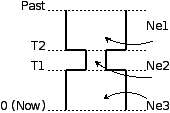
\includegraphics{bottle.png}

在我们的第一个示例中,将生成一个单一种群固定群体大小(Single population, constant size)模板,样本大小(sample size)为30,同群种大小(deme size)为500。代码如下:
\DUspan{keyword,namespace}{}\DUspan{name,namespace}{}\DUspan{keyword,namespace}{}\DUspan{name}{}\DUspan{name}{}\DUspan{punctuation}{}\DUspan{literal,string}{}\DUspan{punctuation}{}\DUspan{punctuation}{}\DUspan{literal,number,integer}{}\DUspan{punctuation}{}\DUspan{punctuation}{}\DUspan{literal,string}{}\DUspan{punctuation}{}\DUspan{punctuation}{}\DUspan{literal,number,integer}{}\DUspan{punctuation}{}\DUspan{literal,number,float}{}\DUspan{punctuation}{}\DUspan{literal,number,float}{}\DUspan{punctuation}{}\DUspan{punctuation}{}\DUspan{literal,string}{}\DUspan{punctuation}{}\DUspan{punctuation}{}\DUspan{literal,number,integer}{}\DUspan{punctuation}{}\DUspan{punctuation}{}\DUspan{literal,string}{}\DUspan{punctuation}{}\DUspan{punctuation}{}\DUspan{literal,number,integer}{}\DUspan{punctuation}{}
\begin{Verbatim}[commandchars=\\\{\}]
\PYG{k+kn}{from} \PYG{n+nn}{Bio.PopGen.SimCoal.Template} \PYG{k+kn}{import} \PYG{n}{generate\PYGZus{}simcoal\PYGZus{}from\PYGZus{}template}

\PYG{n}{generate\PYGZus{}simcoal\PYGZus{}from\PYGZus{}template}\PYG{p}{(}\PYG{l+s}{\PYGZsq{}}\PYG{l+s}{simple}\PYG{l+s}{\PYGZsq{}}\PYG{p}{,}
    \PYG{p}{[}\PYG{p}{(}\PYG{l+m+mi}{1}\PYG{p}{,} \PYG{p}{[}\PYG{p}{(}\PYG{l+s}{\PYGZsq{}}\PYG{l+s}{SNP}\PYG{l+s}{\PYGZsq{}}\PYG{p}{,} \PYG{p}{[}\PYG{l+m+mi}{24}\PYG{p}{,} \PYG{l+m+mf}{0.0005}\PYG{p}{,} \PYG{l+m+mf}{0.0}\PYG{p}{]}\PYG{p}{)}\PYG{p}{]}\PYG{p}{)}\PYG{p}{]}\PYG{p}{,}
    \PYG{p}{[}\PYG{p}{(}\PYG{l+s}{\PYGZsq{}}\PYG{l+s}{sample\PYGZus{}size}\PYG{l+s}{\PYGZsq{}}\PYG{p}{,} \PYG{p}{[}\PYG{l+m+mi}{30}\PYG{p}{]}\PYG{p}{)}\PYG{p}{,}
    \PYG{p}{(}\PYG{l+s}{\PYGZsq{}}\PYG{l+s}{pop\PYGZus{}size}\PYG{l+s}{\PYGZsq{}}\PYG{p}{,} \PYG{p}{[}\PYG{l+m+mi}{100}\PYG{p}{]}\PYG{p}{)}\PYG{p}{]}\PYG{p}{)}
\end{Verbatim}

执行该段代码将会在当前目录生成一个名为simple\_100\_300.par的文件,该文件可作为SIMCOAL2的输入文件,用于模拟群体(下面将会展示Biopython是如何调用SIMCOAL2)。

这段代码仅包含一个函数的调用,让我们一个参数一个参数地讨论。

第一个参数是模板id(从上面的模板列表中选择)。我们使用 ’simple’,表示的是单一群体固定种群大小模板。

第二个参数是染色体结构,将在下一节详细阐述。

第三个参数是所有需要的参数列表及其所有可能的值(此列中所有的参数都只含有一个可能值)。

现在让我们看看岛屿模型示例。我们希望生成几个岛屿模型,并对不同大小的同群种感兴趣:10、50和100,迁移率为1\%。样本大小和同群种大小与上一个示例一致,代码如下:
\DUspan{keyword,namespace}{}\DUspan{name,namespace}{}\DUspan{keyword,namespace}{}\DUspan{name}{}\DUspan{name}{}\DUspan{punctuation}{}\DUspan{literal,string}{}\DUspan{punctuation}{}\DUspan{punctuation}{}\DUspan{literal,number,integer}{}\DUspan{punctuation}{}\DUspan{punctuation}{}\DUspan{literal,string}{}\DUspan{punctuation}{}\DUspan{punctuation}{}\DUspan{literal,number,integer}{}\DUspan{punctuation}{}\DUspan{literal,number,float}{}\DUspan{punctuation}{}\DUspan{literal,number,float}{}\DUspan{punctuation}{}\DUspan{punctuation}{}\DUspan{literal,string}{}\DUspan{punctuation}{}\DUspan{punctuation}{}\DUspan{literal,number,integer}{}\DUspan{punctuation}{}\DUspan{punctuation}{}\DUspan{literal,string}{}\DUspan{punctuation}{}\DUspan{punctuation}{}\DUspan{literal,number,integer}{}\DUspan{punctuation}{}\DUspan{punctuation}{}\DUspan{literal,string}{}\DUspan{punctuation}{}\DUspan{punctuation}{}\DUspan{literal,number,float}{}\DUspan{punctuation}{}\DUspan{punctuation}{}\DUspan{literal,string}{}\DUspan{punctuation}{}\DUspan{punctuation}{}\DUspan{literal,number,integer}{}\DUspan{punctuation}{}\DUspan{literal,number,integer}{}\DUspan{punctuation}{}\DUspan{literal,number,integer}{}\DUspan{punctuation}{}
\begin{Verbatim}[commandchars=\\\{\}]
\PYG{k+kn}{from} \PYG{n+nn}{Bio.PopGen.SimCoal.Template} \PYG{k+kn}{import} \PYG{n}{generate\PYGZus{}simcoal\PYGZus{}from\PYGZus{}template}

\PYG{n}{generate\PYGZus{}simcoal\PYGZus{}from\PYGZus{}template}\PYG{p}{(}\PYG{l+s}{\PYGZsq{}}\PYG{l+s}{island}\PYG{l+s}{\PYGZsq{}}\PYG{p}{,}
    \PYG{p}{[}\PYG{p}{(}\PYG{l+m+mi}{1}\PYG{p}{,} \PYG{p}{[}\PYG{p}{(}\PYG{l+s}{\PYGZsq{}}\PYG{l+s}{SNP}\PYG{l+s}{\PYGZsq{}}\PYG{p}{,} \PYG{p}{[}\PYG{l+m+mi}{24}\PYG{p}{,} \PYG{l+m+mf}{0.0005}\PYG{p}{,} \PYG{l+m+mf}{0.0}\PYG{p}{]}\PYG{p}{)}\PYG{p}{]}\PYG{p}{)}\PYG{p}{]}\PYG{p}{,}
    \PYG{p}{[}\PYG{p}{(}\PYG{l+s}{\PYGZsq{}}\PYG{l+s}{sample\PYGZus{}size}\PYG{l+s}{\PYGZsq{}}\PYG{p}{,} \PYG{p}{[}\PYG{l+m+mi}{30}\PYG{p}{]}\PYG{p}{)}\PYG{p}{,}
    \PYG{p}{(}\PYG{l+s}{\PYGZsq{}}\PYG{l+s}{pop\PYGZus{}size}\PYG{l+s}{\PYGZsq{}}\PYG{p}{,} \PYG{p}{[}\PYG{l+m+mi}{100}\PYG{p}{]}\PYG{p}{)}\PYG{p}{,}
    \PYG{p}{(}\PYG{l+s}{\PYGZsq{}}\PYG{l+s}{mig}\PYG{l+s}{\PYGZsq{}}\PYG{p}{,} \PYG{p}{[}\PYG{l+m+mf}{0.01}\PYG{p}{]}\PYG{p}{)}\PYG{p}{,}
    \PYG{p}{(}\PYG{l+s}{\PYGZsq{}}\PYG{l+s}{total\PYGZus{}demes}\PYG{l+s}{\PYGZsq{}}\PYG{p}{,} \PYG{p}{[}\PYG{l+m+mi}{10}\PYG{p}{,} \PYG{l+m+mi}{50}\PYG{p}{,} \PYG{l+m+mi}{100}\PYG{p}{]}\PYG{p}{)}\PYG{p}{]}\PYG{p}{)}
\end{Verbatim}

此例将会生成3个文件:island\_100\_0.01\_100\_30.par,island\_10\_0.01\_100\_30.par 和 island\_50\_0.01\_100\_30.par。注意,生成文件名的规律是:模板名,然后是参数值逆序排列。

还有一些存在较多争议的群体模板(请见Biopython源代码中Bio/PopGen/SimCoal/data文件夹)。同时,用户可以创建新的模板,该功能将在以后的文档中讨论。


\subsubsection{12.2.1.2  染色体结构}
\label{chr12:id2}
我们强烈建议你阅读SIMCOAL2文档,以完整理解染色体结构建模的各种使用。在本小节,我们只讨论如何使用Biopython接口实现指定的染色体结构,不会涉及SIMCOAL2可实现哪些染色体结构。

我们首先实现一条染色体,包含24个SNPs,每个相邻基因座的重组率为0.0005,次等位基因的最小频率为0。这些由以下列表指定(作为第二个参数传递给generate\_simcoal\_from\_template函数):
\DUspan{punctuation}{}\DUspan{literal,number,integer}{}\DUspan{punctuation}{}\DUspan{punctuation}{}\DUspan{literal,string}{}\DUspan{punctuation}{}\DUspan{punctuation}{}\DUspan{literal,number,integer}{}\DUspan{punctuation}{}\DUspan{literal,number,float}{}\DUspan{punctuation}{}\DUspan{literal,number,float}{}\DUspan{punctuation}{}
\begin{Verbatim}[commandchars=\\\{\}]
\PYG{p}{[}\PYG{p}{(}\PYG{l+m+mi}{1}\PYG{p}{,} \PYG{p}{[}\PYG{p}{(}\PYG{l+s}{\PYGZsq{}}\PYG{l+s}{SNP}\PYG{l+s}{\PYGZsq{}}\PYG{p}{,} \PYG{p}{[}\PYG{l+m+mi}{24}\PYG{p}{,} \PYG{l+m+mf}{0.0005}\PYG{p}{,} \PYG{l+m+mf}{0.0}\PYG{p}{]}\PYG{p}{)}\PYG{p}{]}\PYG{p}{)}\PYG{p}{]}
\end{Verbatim}

这实际上是上一个示例使用的染色体结构。

染色体结构表示为一个包含所有染色体的列表,每条染色体(即列表中的每个元素)由一个元组(tuple)组成,元组包括一对元素组成。元组的第一个元素是染色体被重复的次数(因为有可能需要多次重复同一条染色体)。元组的第二个元素是一个表示该染色体的实际组成的列表,每个列表元素又包括一对元素,第一个是基因座类型,第二个是该基因座的参数列表。是否有点混淆了呢?在我们展示示例之前,先让我们回顾下上一个示例:我们有一个列表(表示一条染色体),该染色体只有一个实例(因此不会被重复),它由24个SNPs组成,每个相邻SNP间的重组率为0.0005,次等位基因的最小频率为0.0(即它可以在某些染色体中缺失)。

现在让我们看看更复杂的示例:
\DUspan{punctuation}{}\DUspan{punctuation}{}\DUspan{literal,number,integer}{}\DUspan{punctuation}{}\DUspan{punctuation}{}\DUspan{punctuation}{}\DUspan{literal,string}{}\DUspan{punctuation}{}\DUspan{punctuation}{}\DUspan{literal,number,integer}{}\DUspan{punctuation}{}\DUspan{literal,number,float}{}\DUspan{punctuation}{}\DUspan{literal,number,float}{}\DUspan{punctuation}{}\DUspan{punctuation}{}\DUspan{punctuation}{}\DUspan{punctuation}{}\DUspan{literal,number,integer}{}\DUspan{punctuation}{}\DUspan{punctuation}{}\DUspan{punctuation}{}\DUspan{literal,string}{}\DUspan{punctuation}{}\DUspan{punctuation}{}\DUspan{literal,number,integer}{}\DUspan{punctuation}{}\DUspan{literal,number,float}{}\DUspan{punctuation}{}\DUspan{literal,number,float}{}\DUspan{punctuation}{}\DUspan{literal,number,float}{}\DUspan{punctuation}{}\DUspan{punctuation}{}\DUspan{literal,string}{}\DUspan{punctuation}{}\DUspan{punctuation}{}\DUspan{literal,number,integer}{}\DUspan{punctuation}{}\DUspan{literal,number,float}{}\DUspan{punctuation}{}\DUspan{literal,number,float}{}\DUspan{punctuation}{}\DUspan{punctuation}{}\DUspan{literal,string}{}\DUspan{punctuation}{}\DUspan{punctuation}{}\DUspan{literal,number,integer}{}\DUspan{punctuation}{}\DUspan{literal,number,float}{}\DUspan{punctuation}{}\DUspan{literal,number,float}{}\DUspan{punctuation}{}\DUspan{literal,number,float}{}\DUspan{punctuation}{}\DUspan{literal,number,float}{}\DUspan{punctuation}{}\DUspan{punctuation}{}\DUspan{punctuation}{}\DUspan{punctuation}{}
\begin{Verbatim}[commandchars=\\\{\}]
\PYG{p}{[}
  \PYG{p}{(}\PYG{l+m+mi}{5}\PYG{p}{,} \PYG{p}{[}
       \PYG{p}{(}\PYG{l+s}{\PYGZsq{}}\PYG{l+s}{SNP}\PYG{l+s}{\PYGZsq{}}\PYG{p}{,} \PYG{p}{[}\PYG{l+m+mi}{24}\PYG{p}{,} \PYG{l+m+mf}{0.0005}\PYG{p}{,} \PYG{l+m+mf}{0.0}\PYG{p}{]}\PYG{p}{)}
      \PYG{p}{]}
  \PYG{p}{)}\PYG{p}{,}
  \PYG{p}{(}\PYG{l+m+mi}{2}\PYG{p}{,} \PYG{p}{[}
       \PYG{p}{(}\PYG{l+s}{\PYGZsq{}}\PYG{l+s}{DNA}\PYG{l+s}{\PYGZsq{}}\PYG{p}{,} \PYG{p}{[}\PYG{l+m+mi}{10}\PYG{p}{,} \PYG{l+m+mf}{0.0}\PYG{p}{,} \PYG{l+m+mf}{0.00005}\PYG{p}{,} \PYG{l+m+mf}{0.33}\PYG{p}{]}\PYG{p}{)}\PYG{p}{,}
       \PYG{p}{(}\PYG{l+s}{\PYGZsq{}}\PYG{l+s}{RFLP}\PYG{l+s}{\PYGZsq{}}\PYG{p}{,} \PYG{p}{[}\PYG{l+m+mi}{1}\PYG{p}{,} \PYG{l+m+mf}{0.0}\PYG{p}{,} \PYG{l+m+mf}{0.0001}\PYG{p}{]}\PYG{p}{)}\PYG{p}{,}
       \PYG{p}{(}\PYG{l+s}{\PYGZsq{}}\PYG{l+s}{MICROSAT}\PYG{l+s}{\PYGZsq{}}\PYG{p}{,} \PYG{p}{[}\PYG{l+m+mi}{1}\PYG{p}{,} \PYG{l+m+mf}{0.0}\PYG{p}{,} \PYG{l+m+mf}{0.001}\PYG{p}{,} \PYG{l+m+mf}{0.0}\PYG{p}{,} \PYG{l+m+mf}{0.0}\PYG{p}{]}\PYG{p}{)}
      \PYG{p}{]}
  \PYG{p}{)}
\PYG{p}{]}
\end{Verbatim}

首先,我们有5条与上一示例具有相同结构组成的染色体(即24SNPs)。然后是2条这样的染色体:包含一段具有重组率为0.0、突变率为0.0005及置换率为0.33的10个核苷酸长度的DNA序列,一段具有重组率为0.0、突变率为0.0001的RFLP,一段具有重组率为0.0、突变率为0.001、几何参数为0.0、范围限制参数为0.0的微卫星(microsatellite,STR)序列(注意,因为这是单个微卫星,接下来没有基因座,因此这里的重组率没有任何影响,更多关于这些参数的信息请查阅SIMCOAL2文档,你可以使用它们模拟各种突变模型,包括典型的微卫星渐变突变模型)。


\subsection{12.2.2  运行SIMCOAL2}
\label{chr12:simcoal2}
现在我们讨论如何从Biopython内部运行SIMCOAL2。这需要SIMCOAL2的可执行二进制文件名为simcoal2(在Windows平台下为simcoal2.exe),请注意,从官网下载的程序命名格式通常为simcoal2\_x\_y。因此,当安装SIMCOAL2时,需要重命名可执行文件,这样Biopython才能正确调用。

SIMCOAL2可以处理不是使用上诉方法生成的文件(如手动配置的参数文件),但是我们将使用上述方法得到的文件创建模型:
\DUspan{keyword,namespace}{}\DUspan{name,namespace}{}\DUspan{keyword,namespace}{}\DUspan{name}{}\DUspan{keyword,namespace}{}\DUspan{name,namespace}{}\DUspan{keyword,namespace}{}\DUspan{name}{}\DUspan{name}{}\DUspan{punctuation}{}\DUspan{literal,string}{}\DUspan{punctuation}{}\DUspan{punctuation}{}\DUspan{punctuation}{}\DUspan{literal,number,integer}{}\DUspan{punctuation}{}\DUspan{punctuation}{}\DUspan{punctuation}{}\DUspan{literal,string}{}\DUspan{punctuation}{}\DUspan{punctuation}{}\DUspan{literal,number,integer}{}\DUspan{punctuation}{}\DUspan{literal,number,float}{}\DUspan{punctuation}{}\DUspan{literal,number,float}{}\DUspan{punctuation}{}\DUspan{punctuation}{}\DUspan{punctuation}{}\DUspan{punctuation}{}\DUspan{literal,number,integer}{}\DUspan{punctuation}{}\DUspan{punctuation}{}\DUspan{punctuation}{}\DUspan{literal,string}{}\DUspan{punctuation}{}\DUspan{punctuation}{}\DUspan{literal,number,integer}{}\DUspan{punctuation}{}\DUspan{literal,number,float}{}\DUspan{punctuation}{}\DUspan{literal,number,float}{}\DUspan{punctuation}{}\DUspan{literal,number,float}{}\DUspan{punctuation}{}\DUspan{punctuation}{}\DUspan{literal,string}{}\DUspan{punctuation}{}\DUspan{punctuation}{}\DUspan{literal,number,integer}{}\DUspan{punctuation}{}\DUspan{literal,number,float}{}\DUspan{punctuation}{}\DUspan{literal,number,float}{}\DUspan{punctuation}{}\DUspan{punctuation}{}\DUspan{literal,string}{}\DUspan{punctuation}{}\DUspan{punctuation}{}\DUspan{literal,number,integer}{}\DUspan{punctuation}{}\DUspan{literal,number,float}{}\DUspan{punctuation}{}\DUspan{literal,number,float}{}\DUspan{punctuation}{}\DUspan{literal,number,float}{}\DUspan{punctuation}{}\DUspan{literal,number,float}{}\DUspan{punctuation}{}\DUspan{punctuation}{}\DUspan{punctuation}{}\DUspan{punctuation}{}\DUspan{punctuation}{}\DUspan{literal,string}{}\DUspan{punctuation}{}\DUspan{punctuation}{}\DUspan{literal,number,integer}{}\DUspan{punctuation}{}\DUspan{punctuation}{}\DUspan{literal,string}{}\DUspan{punctuation}{}\DUspan{punctuation}{}\DUspan{literal,number,integer}{}\DUspan{punctuation}{}\DUspan{name}{}\DUspan{operator}{}\DUspan{name}{}\DUspan{punctuation}{}\DUspan{literal,string}{}\DUspan{punctuation}{}\DUspan{name}{}\DUspan{operator}{}\DUspan{name}{}\DUspan{punctuation}{}\DUspan{literal,string}{}\DUspan{punctuation}{}\DUspan{literal,number,integer}{}\DUspan{punctuation}{}
\begin{Verbatim}[commandchars=\\\{\}]
\PYG{k+kn}{from} \PYG{n+nn}{Bio.PopGen.SimCoal.Template} \PYG{k+kn}{import} \PYG{n}{generate\PYGZus{}simcoal\PYGZus{}from\PYGZus{}template}
\PYG{k+kn}{from} \PYG{n+nn}{Bio.PopGen.SimCoal.Controller} \PYG{k+kn}{import} \PYG{n}{SimCoalController}


\PYG{n}{generate\PYGZus{}simcoal\PYGZus{}from\PYGZus{}template}\PYG{p}{(}\PYG{l+s}{\PYGZsq{}}\PYG{l+s}{simple}\PYG{l+s}{\PYGZsq{}}\PYG{p}{,}
    \PYG{p}{[}
      \PYG{p}{(}\PYG{l+m+mi}{5}\PYG{p}{,} \PYG{p}{[}
           \PYG{p}{(}\PYG{l+s}{\PYGZsq{}}\PYG{l+s}{SNP}\PYG{l+s}{\PYGZsq{}}\PYG{p}{,} \PYG{p}{[}\PYG{l+m+mi}{24}\PYG{p}{,} \PYG{l+m+mf}{0.0005}\PYG{p}{,} \PYG{l+m+mf}{0.0}\PYG{p}{]}\PYG{p}{)}
          \PYG{p}{]}
      \PYG{p}{)}\PYG{p}{,}
      \PYG{p}{(}\PYG{l+m+mi}{2}\PYG{p}{,} \PYG{p}{[}
           \PYG{p}{(}\PYG{l+s}{\PYGZsq{}}\PYG{l+s}{DNA}\PYG{l+s}{\PYGZsq{}}\PYG{p}{,} \PYG{p}{[}\PYG{l+m+mi}{10}\PYG{p}{,} \PYG{l+m+mf}{0.0}\PYG{p}{,} \PYG{l+m+mf}{0.00005}\PYG{p}{,} \PYG{l+m+mf}{0.33}\PYG{p}{]}\PYG{p}{)}\PYG{p}{,}
           \PYG{p}{(}\PYG{l+s}{\PYGZsq{}}\PYG{l+s}{RFLP}\PYG{l+s}{\PYGZsq{}}\PYG{p}{,} \PYG{p}{[}\PYG{l+m+mi}{1}\PYG{p}{,} \PYG{l+m+mf}{0.0}\PYG{p}{,} \PYG{l+m+mf}{0.0001}\PYG{p}{]}\PYG{p}{)}\PYG{p}{,}
           \PYG{p}{(}\PYG{l+s}{\PYGZsq{}}\PYG{l+s}{MICROSAT}\PYG{l+s}{\PYGZsq{}}\PYG{p}{,} \PYG{p}{[}\PYG{l+m+mi}{1}\PYG{p}{,} \PYG{l+m+mf}{0.0}\PYG{p}{,} \PYG{l+m+mf}{0.001}\PYG{p}{,} \PYG{l+m+mf}{0.0}\PYG{p}{,} \PYG{l+m+mf}{0.0}\PYG{p}{]}\PYG{p}{)}
          \PYG{p}{]}
      \PYG{p}{)}
    \PYG{p}{]}\PYG{p}{,}
    \PYG{p}{[}\PYG{p}{(}\PYG{l+s}{\PYGZsq{}}\PYG{l+s}{sample\PYGZus{}size}\PYG{l+s}{\PYGZsq{}}\PYG{p}{,} \PYG{p}{[}\PYG{l+m+mi}{30}\PYG{p}{]}\PYG{p}{)}\PYG{p}{,}
    \PYG{p}{(}\PYG{l+s}{\PYGZsq{}}\PYG{l+s}{pop\PYGZus{}size}\PYG{l+s}{\PYGZsq{}}\PYG{p}{,} \PYG{p}{[}\PYG{l+m+mi}{100}\PYG{p}{]}\PYG{p}{)}\PYG{p}{]}\PYG{p}{)}

\PYG{n}{ctrl} \PYG{o}{=} \PYG{n}{SimCoalController}\PYG{p}{(}\PYG{l+s}{\PYGZsq{}}\PYG{l+s}{.}\PYG{l+s}{\PYGZsq{}}\PYG{p}{)}
\PYG{n}{ctrl}\PYG{o}{.}\PYG{n}{run\PYGZus{}simcoal}\PYG{p}{(}\PYG{l+s}{\PYGZsq{}}\PYG{l+s}{simple\PYGZus{}100\PYGZus{}30.par}\PYG{l+s}{\PYGZsq{}}\PYG{p}{,} \PYG{l+m+mi}{50}\PYG{p}{)}
\end{Verbatim}

需要注意的是最后两行(以及新增的import行)。首先是创建一个应用程序控制器对象,需要指定二进制可执行文件所在路径。

模拟器在最后一行运行:从上述阐述的规律可知,文件名为simple\_100\_30.par的输入文件是我们创建的模拟参数文件,然后我们指定了希望运行50次独立模拟。默认情况下,Biopython模拟二倍体数据,但是可以添加第三个参数用于模拟单倍体数据(字符串`0')。然后,SIMCOAL2将会执行(这需要运行很长时间),并创建一个包含模拟结果的文件夹,结果文件可便可用于分析(尤其是研究Arlequin3数据)。在未来的Biopython版本中,可能会支持Arlequin3格式文件的读取,从而在Biopython中便能分析SIMCOAL2结果。


\section{12.3  其它应用程序}
\label{chr12:id3}
这里我们讨论一些处理其它的群体遗传学中应用程序的接口和小工具,这些应用程序具有争议,使用得较少。


\subsection{12.3.1  FDist:检测选择压力和分子适应}
\label{chr12:fdist}
FDist是一个选择压力检测的应用程序包,基于通过 $F_{st}$ 和杂合度计算(即模拟)得到的“中性”(“neutral”)置信区间。“中性”置信区间外的Markers(可以是SNPs,微卫星,AFLPs等等)可以被认为是候选的受选择marker。

FDist主要运用在当marker数量足够用于估计平均 $F_{st}$ ,而不足以从数据集中计算出离群点 - 直接地或者在知道大多数marker在基因组中的相对位置的情况下使用基于如Extended Haplotype Heterozygosity (EHH)的方法。

典型的FDist的使用如下:
\begin{enumerate}
\item {} 
从其它格式读取数据为FDist格式;

\item {} 
计算平均 $F_{st}$ ,由FDist的datacal完成;

\item {} 
根据平均 $F_{st}$ 和期望的总群体数模拟“中性”markers,这是核心部分,由FDist的fdist完成;

\item {} 
根据指定的置信范围(通常是95\%或者是99\%)计算置信区间,由cplot完成,主要用于对区间作图;

\item {} 
用模拟的“中性”置信区间评估每个Marker的状态,由pv完成,用于检测每个marker与模拟的相比的离群状态;

\end{enumerate}

我们将以示例代码讨论每一步(FDist可执行二进制文件需要在PATH环境变量中)。

FDist数据格式是该应用程序特有的,不被其它应用程序使用。因此你需要转化你的数据格式到FDist可使用的格式。Biopython可以帮助你完成这个过程。这里有一个将GenePop格式转换为FDist格式的示例(同时包括后面示例将用到的import语句):
\DUspan{keyword,namespace}{}\DUspan{name,namespace}{}\DUspan{keyword,namespace}{}\DUspan{name}{}\DUspan{keyword,namespace}{}\DUspan{name,namespace}{}\DUspan{keyword,namespace}{}\DUspan{name}{}\DUspan{keyword,namespace}{}\DUspan{name,namespace}{}\DUspan{keyword,namespace}{}\DUspan{name}{}\DUspan{keyword,namespace}{}\DUspan{name,namespace}{}\DUspan{keyword,namespace}{}\DUspan{name}{}\DUspan{name}{}\DUspan{operator}{}\DUspan{name}{}\DUspan{operator}{}\DUspan{name}{}\DUspan{punctuation}{}\DUspan{name,builtin}{}\DUspan{punctuation}{}\DUspan{literal,string}{}\DUspan{punctuation}{}\DUspan{name}{}\DUspan{operator}{}\DUspan{name}{}\DUspan{punctuation}{}\DUspan{name}{}\DUspan{punctuation}{}\DUspan{name}{}\DUspan{operator}{}\DUspan{name,builtin}{}\DUspan{punctuation}{}\DUspan{literal,string}{}\DUspan{punctuation}{}\DUspan{literal,string}{}\DUspan{punctuation}{}\DUspan{name}{}\DUspan{operator}{}\DUspan{name}{}\DUspan{punctuation}{}\DUspan{name,builtin}{}\DUspan{punctuation}{}\DUspan{name}{}\DUspan{punctuation}{}\DUspan{name}{}\DUspan{operator}{}\DUspan{name}{}\DUspan{punctuation}{}
\begin{Verbatim}[commandchars=\\\{\}]
\PYG{k+kn}{from} \PYG{n+nn}{Bio.PopGen} \PYG{k+kn}{import} \PYG{n}{GenePop}
\PYG{k+kn}{from} \PYG{n+nn}{Bio.PopGen} \PYG{k+kn}{import} \PYG{n}{FDist}
\PYG{k+kn}{from} \PYG{n+nn}{Bio.PopGen.FDist} \PYG{k+kn}{import} \PYG{n}{Controller}
\PYG{k+kn}{from} \PYG{n+nn}{Bio.PopGen.FDist.Utils} \PYG{k+kn}{import} \PYG{n}{convert\PYGZus{}genepop\PYGZus{}to\PYGZus{}fdist}

\PYG{n}{gp\PYGZus{}rec} \PYG{o}{=} \PYG{n}{GenePop}\PYG{o}{.}\PYG{n}{read}\PYG{p}{(}\PYG{n+nb}{open}\PYG{p}{(}\PYG{l+s}{\PYGZdq{}}\PYG{l+s}{example.gen}\PYG{l+s}{\PYGZdq{}}\PYG{p}{)}\PYG{p}{)}
\PYG{n}{fd\PYGZus{}rec} \PYG{o}{=} \PYG{n}{convert\PYGZus{}genepop\PYGZus{}to\PYGZus{}fdist}\PYG{p}{(}\PYG{n}{gp\PYGZus{}rec}\PYG{p}{)}
\PYG{n}{in\PYGZus{}file} \PYG{o}{=} \PYG{n+nb}{open}\PYG{p}{(}\PYG{l+s}{\PYGZdq{}}\PYG{l+s}{infile}\PYG{l+s}{\PYGZdq{}}\PYG{p}{,} \PYG{l+s}{\PYGZdq{}}\PYG{l+s}{w}\PYG{l+s}{\PYGZdq{}}\PYG{p}{)}
\PYG{n}{in\PYGZus{}file}\PYG{o}{.}\PYG{n}{write}\PYG{p}{(}\PYG{n+nb}{str}\PYG{p}{(}\PYG{n}{fd\PYGZus{}rec}\PYG{p}{)}\PYG{p}{)}
\PYG{n}{in\PYGZus{}file}\PYG{o}{.}\PYG{n}{close}\PYG{p}{(}\PYG{p}{)}
\end{Verbatim}

在该段代码中,我们解析GenePop文件并转化为FDist记录(record)。

输出FDist记录将得到可以直接保存到可用于FDist的文件的字符串。FDist需要输入文件名为infile,因此我们将记录保存到文件名为infile的文件。

FDist记录最重要的字段(field)是:num\_pops,群体数量;num\_loci,基因座数量和loci\_data,marker数据。记录的许多信息对用户来说可能没有用处,仅用于传递给FDist。

下一步是计算平均数据集的 $F_{st}$ (以及样本大小):
\DUspan{name}{}\DUspan{operator}{}\DUspan{name}{}\DUspan{operator}{}\DUspan{name}{}\DUspan{punctuation}{}\DUspan{name}{}\DUspan{punctuation}{}\DUspan{name}{}\DUspan{operator}{}\DUspan{name}{}\DUspan{operator}{}\DUspan{name}{}\DUspan{punctuation}{}
\begin{Verbatim}[commandchars=\\\{\}]
\PYG{n}{ctrl} \PYG{o}{=} \PYG{n}{Controller}\PYG{o}{.}\PYG{n}{FDistController}\PYG{p}{(}\PYG{p}{)}
\PYG{n}{fst}\PYG{p}{,} \PYG{n}{samp\PYGZus{}size} \PYG{o}{=} \PYG{n}{ctrl}\PYG{o}{.}\PYG{n}{run\PYGZus{}datacal}\PYG{p}{(}\PYG{p}{)}
\end{Verbatim}

第一行我们创建了一个控制调用FDist软件包的对象,该对象被用于调用该包的其它应用程序。

第二行我们调用datacal应用程序,它用于计算 $F_{st}$ 和样本大小。值得注意的是,用datacal计算得到的 $F_{st}$ 是 Weir-Cockerham \(\theta\)的“变种”( \emph{variation} )。

现在我们可以调用主程序fdist模拟中性Markers。
\DUspan{name}{}\DUspan{operator}{}\DUspan{name}{}\DUspan{operator}{}\DUspan{name}{}\DUspan{punctuation}{}\DUspan{name}{}\DUspan{operator}{}\DUspan{literal,number,integer}{}\DUspan{punctuation}{}\DUspan{name}{}\DUspan{operator}{}\DUspan{name}{}\DUspan{operator}{}\DUspan{name}{}\DUspan{punctuation}{}\DUspan{name}{}\DUspan{operator}{}\DUspan{name}{}\DUspan{punctuation}{}\DUspan{name}{}\DUspan{operator}{}\DUspan{name}{}\DUspan{punctuation}{}\DUspan{name}{}\DUspan{operator}{}\DUspan{literal,number,integer}{}\DUspan{punctuation}{}\DUspan{name}{}\DUspan{operator}{}\DUspan{literal,number,integer}{}\DUspan{punctuation}{}
\begin{Verbatim}[commandchars=\\\{\}]
\PYG{n}{sim\PYGZus{}fst} \PYG{o}{=} \PYG{n}{ctrl}\PYG{o}{.}\PYG{n}{run\PYGZus{}fdist}\PYG{p}{(}\PYG{n}{npops} \PYG{o}{=} \PYG{l+m+mi}{15}\PYG{p}{,} \PYG{n}{nsamples} \PYG{o}{=} \PYG{n}{fd\PYGZus{}rec}\PYG{o}{.}\PYG{n}{num\PYGZus{}pops}\PYG{p}{,} \PYG{n}{fst} \PYG{o}{=} \PYG{n}{fst}\PYG{p}{,}
    \PYG{n}{sample\PYGZus{}size} \PYG{o}{=} \PYG{n}{samp\PYGZus{}size}\PYG{p}{,} \PYG{n}{mut} \PYG{o}{=} \PYG{l+m+mi}{0}\PYG{p}{,} \PYG{n}{num\PYGZus{}sims} \PYG{o}{=} \PYG{l+m+mi}{40000}\PYG{p}{)}
\end{Verbatim}
\begin{description}
\item[{\textbf{npops}}] \leavevmode
现存自然群体数量,完全是一个“瞎猜值”(“guestimate”),必须小于100。

\item[{\textbf{nsamples}}] \leavevmode
抽样群体数量,需要小于npops。

\item[{\textbf{fst}}] \leavevmode
平均 $F_{st}$ 。

\item[{\textbf{sample\_size}}] \leavevmode
每个群体抽样个体平均数

\item[{\textbf{mut}}] \leavevmode
突变模型:0 - 无限等位基因突变模型;1 - 渐变突变模型

\item[{\textbf{num\_sims}}] \leavevmode
执行模拟的次数。通常,40000左右的数值即可,但是如果得到的执行区间范围比较大(可以通过下面的置信区间作图检测到),可以上调此值(建议每次调整10000次模拟)。

\end{description}

样本数量和样本大小措辞上的混乱源于原始的应用程序。

将会得到一个名为out.dat的文件,它包含模拟的杂合度和 $F_{st}$ 值,行数与模拟的次数相同。

注意,fdist返回它可以模拟的平均 $F_{st}$ ,关于此问题更多的细节,请阅读下面的“估计期望的平均 $F_{st}$ ”

下一步(可选步骤)是计算置信区间:
\DUspan{name}{}\DUspan{operator}{}\DUspan{name}{}\DUspan{operator}{}\DUspan{name}{}\DUspan{punctuation}{}\DUspan{name}{}\DUspan{operator}{}\DUspan{literal,number,float}{}\DUspan{punctuation}{}
\begin{Verbatim}[commandchars=\\\{\}]
\PYG{n}{cpl\PYGZus{}interval} \PYG{o}{=} \PYG{n}{ctrl}\PYG{o}{.}\PYG{n}{run\PYGZus{}cplot}\PYG{p}{(}\PYG{n}{ci}\PYG{o}{=}\PYG{l+m+mf}{0.99}\PYG{p}{)}
\end{Verbatim}

只能在运行fdist之后才能调用cplot。

这将计算先前fdist结果的置信区间(此例中为99\%)。第一个元素是杂合度,第二个是该杂合度的 $F_{st}$ 置信下限,第三个是 $F_{st}$ 平均值,第四个是置信上限。可以用于记录置信区间等高线。该列表也可以输出到out.cpl文件。

这步的主要目的是返回一系列的点用于对置信区间作图。如果只是需要根据模拟结果对每个marker的状态进行评估,可以跳过此步。
\DUspan{name}{}\DUspan{operator}{}\DUspan{name}{}\DUspan{operator}{}\DUspan{name}{}\DUspan{punctuation}{}
\begin{Verbatim}[commandchars=\\\{\}]
\PYG{n}{pv\PYGZus{}data} \PYG{o}{=} \PYG{n}{ctrl}\PYG{o}{.}\PYG{n}{run\PYGZus{}pv}\PYG{p}{(}\PYG{p}{)}
\end{Verbatim}

只能在运行fdist之后才能调用pv。

这将使用模拟marker对每个个体真实的marker进行评估,并返回一个列表,顺序与FDist记录中loci\_list一致(loci\_list又与GenePop顺序一致)。列表中每个元素包含四个元素,其中最重要的是最后一个元素(关于其他的元素,为了简单起见,我们不在这里讨论,请见pv帮助文档),它返回模拟的 $F_{st}$ 低于 marker $F_{st}$ 的概率。较大值说明极有可能是正选择(positive selection)marker,较小值表明可能是平衡选择(balancing selection)marker,中间值则可能是中性marker。怎样的值是“较大值”、“较小值”或者“中间值”是一个很主观的问题,但当使用置信区间方法及95\%的置信区间时,“较大值”在0.95 - 1.00之间,“较小值”在0.00 - 0.05之间,“中间值”在0.05 - 0.05之间。


\subsubsection{12.3.1.1  估计期望的平均 $F_{st}$}
\label{chr12:id4}
FDist通过对由下例公式得到的迁移率进行溯祖模拟估计期望的平均 $F_{st}$ :
\begin{gather}
\begin{split}N_{m} = \frac{1 - F_{st}}{4F_{st}}\end{split}\notag
\end{gather}
该公式有一些前提,比如种群大小无限大。

在实践中,当群体数量比较小,突变模型为渐进突变模型,样本大小增加,fdist将不能模拟得到可接受的近似平均 $F_{st}$ 。

为了解决这个问题,Biopython提供了一个使用迭代方法的函数,通过依次运行几个fdist得到期望的值。该方法比运行单个fdist相比耗费更多计算资源,但是可以得到更好的结果。以下代码运行fdist得到期望的 $F_{st}$ :
\DUspan{name}{}\DUspan{operator}{}\DUspan{name}{}\DUspan{operator}{}\DUspan{name}{}\DUspan{punctuation}{}\DUspan{name}{}\DUspan{operator}{}\DUspan{literal,number,integer}{}\DUspan{punctuation}{}\DUspan{name}{}\DUspan{operator}{}\DUspan{name}{}\DUspan{operator}{}\DUspan{name}{}\DUspan{punctuation}{}\DUspan{name}{}\DUspan{operator}{}\DUspan{name}{}\DUspan{punctuation}{}\DUspan{name}{}\DUspan{operator}{}\DUspan{name}{}\DUspan{punctuation}{}\DUspan{name}{}\DUspan{operator}{}\DUspan{literal,number,integer}{}\DUspan{punctuation}{}\DUspan{name}{}\DUspan{operator}{}\DUspan{literal,number,integer}{}\DUspan{punctuation}{}\DUspan{name}{}\DUspan{operator}{}\DUspan{literal,number,float}{}\DUspan{punctuation}{}
\begin{Verbatim}[commandchars=\\\{\}]
\PYG{n}{sim\PYGZus{}fst} \PYG{o}{=} \PYG{n}{ctrl}\PYG{o}{.}\PYG{n}{run\PYGZus{}fdist\PYGZus{}force\PYGZus{}fst}\PYG{p}{(}\PYG{n}{npops} \PYG{o}{=} \PYG{l+m+mi}{15}\PYG{p}{,} \PYG{n}{nsamples} \PYG{o}{=} \PYG{n}{fd\PYGZus{}rec}\PYG{o}{.}\PYG{n}{num\PYGZus{}pops}\PYG{p}{,}
    \PYG{n}{fst} \PYG{o}{=} \PYG{n}{fst}\PYG{p}{,} \PYG{n}{sample\PYGZus{}size} \PYG{o}{=} \PYG{n}{samp\PYGZus{}size}\PYG{p}{,} \PYG{n}{mut} \PYG{o}{=} \PYG{l+m+mi}{0}\PYG{p}{,} \PYG{n}{num\PYGZus{}sims} \PYG{o}{=} \PYG{l+m+mi}{40000}\PYG{p}{,}
    \PYG{n}{limit} \PYG{o}{=} \PYG{l+m+mf}{0.05}\PYG{p}{)}
\end{Verbatim}

与run\_fdist相比,唯一一个新的可选参数是limit,它表示期望的最大错误率。run\_fdist可以(或许应该)由run\_fdist\_force\_fst替代。


\subsubsection{12.3.1.2  说明}
\label{chr12:id5}
计算平均 $F_{st}$ 的过程可能比这里呈现的要复杂得多。更多的信息请查阅FDist README文件。同时,Biopython的代码也可用于实现更复杂的过程。


\section{12.4  未来发展}
\label{chr12:id6}
最期望的是您的参与!

尽管如此,已经完成的功能模块正在逐步加入到Bio.PopGen,这些代码覆盖了程序FDist和SimCoal2,HapMap和UCSC Table Browser数据库,以及一些简单的统计计算,如 $F_{st}$ , 或等位基因数。


\chapter{第13章  Bio.Phylo系统发育分析}
\label{chr13:bio-phylo}\label{chr13::doc}\label{chr13:chapter-phylo}
Biopython1.54开始引入了Bio.Phylo模块,与SeqIO和AlignIO类似,它的目的是提供
一个通用的独立于源数据格式的方法来使用系统进化树,同时提供一致的API来进行
I/O操作。

Bio.Phylo在一篇开放获取的期刊文章中有介绍
{[}{\hyperref[chr23:talevich2012]{\emph{9}}}, Talevich \emph{et al.}, 2012{]}, 这可能对您也有所帮助。


\section{13.1  示例: 树中有什么?}
\label{chr13:id1}
为了熟悉这个模块,让我们首先从一个已经创建好的树开始,从几个不同的角度来审视
它。接着我们将给树的分支上颜色,并使用一个特殊的phyloXML特性,最终保存树。

译者注:本翻译中, \textbf{分支} 对应原文中的 \textbf{branch} ,原文中一般代表
某一个节点的前导连线;而 \textbf{进化枝} 对应原文中的 \textbf{clade} ,代表某个节点所代表的整个
进化分支,包括本身和它所有的后代;若clade代表biopython中的对象则保留原文

在终端中使用你喜欢的编辑器创建一个简单的Newick文件:
\DUspan{operator}{}\DUspan{name}{}\DUspan{operator}{}\DUspan{name}{}\DUspan{operator}{}\DUspan{name}{}\DUspan{operator}{}\DUspan{name}{}\DUspan{operator}{}\DUspan{punctuation}{}\DUspan{name}{}\DUspan{punctuation}{}\DUspan{name}{}\DUspan{punctuation}{}\DUspan{name}{}\DUspan{punctuation}{}\DUspan{name}{}\DUspan{punctuation}{}\DUspan{name}{}\DUspan{punctuation}{}\DUspan{name}{}\DUspan{punctuation}{}\DUspan{name}{}\DUspan{punctuation}{}\DUspan{operator}{}\DUspan{name}{}
\begin{Verbatim}[commandchars=\\\{\}]
\% cat \textgreater{} simple.dnd \textless{}\textless{}EOF
\textgreater{} (((A,B),(C,D)),(E,F,G));
\textgreater{} EOF
\end{Verbatim}

这棵树没有分支长度,只有一个拓扑结构和标记的端点。(如果你有一个真正的树文件,
你也可以使用它来替代进行示例操作。)

选择启动你的Python解释器:
\DUspan{operator}{}\DUspan{name}{}\DUspan{operator}{}\DUspan{name}{}
\begin{Verbatim}[commandchars=\\\{\}]
\% ipython -pylab
\end{Verbatim}

对于交互式操作,使用参数 \code{-pylab} 启动IPython解释器能启用 \textbf{matplotlib} 整合
功能,这样图像就能自动弹出来。我们将在这个示例中使用该功能。

现在,在Python终端中,读取树文件,给定文件名和格式名。
\DUspan{operator}{}\DUspan{keyword,namespace}{}\DUspan{name,namespace}{}\DUspan{keyword,namespace}{}\DUspan{name}{}\DUspan{operator}{}\DUspan{name}{}\DUspan{operator}{}\DUspan{name}{}\DUspan{operator}{}\DUspan{name}{}\DUspan{punctuation}{}\DUspan{literal,string}{}\DUspan{punctuation}{}\DUspan{literal,string}{}\DUspan{punctuation}{}
\begin{Verbatim}[commandchars=\\\{\}]
\PYG{g+gp}{\PYGZgt{}\PYGZgt{}\PYGZgt{} }\PYG{k+kn}{from} \PYG{n+nn}{Bio} \PYG{k+kn}{import} \PYG{n}{Phylo}
\PYG{g+gp}{\PYGZgt{}\PYGZgt{}\PYGZgt{} }\PYG{n}{tree} \PYG{o}{=} \PYG{n}{Phylo}\PYG{o}{.}\PYG{n}{read}\PYG{p}{(}\PYG{l+s}{\PYGZdq{}}\PYG{l+s}{simple.dnd}\PYG{l+s}{\PYGZdq{}}\PYG{p}{,} \PYG{l+s}{\PYGZdq{}}\PYG{l+s}{newick}\PYG{l+s}{\PYGZdq{}}\PYG{p}{)}
\end{Verbatim}

以字符串打印该树对象我们将得到整个对象的层次结构概况。
\DUspan{operator}{}\DUspan{keyword}{}\DUspan{name}{}\DUspan{name}{}\DUspan{punctuation}{}\DUspan{name}{}\DUspan{operator}{}\DUspan{literal,number,float}{}\DUspan{punctuation}{}\DUspan{name}{}\DUspan{operator}{}\DUspan{name,builtin,pseudo}{}\DUspan{punctuation}{}\DUspan{name}{}\DUspan{operator}{}\DUspan{literal,string}{}\DUspan{punctuation}{}\DUspan{name}{}\DUspan{punctuation}{}\DUspan{name}{}\DUspan{operator}{}\DUspan{literal,number,float}{}\DUspan{punctuation}{}\DUspan{name}{}\DUspan{punctuation}{}\DUspan{name}{}\DUspan{operator}{}\DUspan{literal,number,float}{}\DUspan{punctuation}{}\DUspan{name}{}\DUspan{punctuation}{}\DUspan{name}{}\DUspan{operator}{}\DUspan{literal,number,float}{}\DUspan{punctuation}{}\DUspan{name}{}\DUspan{punctuation}{}\DUspan{name}{}\DUspan{operator}{}\DUspan{literal,number,float}{}\DUspan{punctuation}{}\DUspan{name}{}\DUspan{operator}{}\DUspan{literal,string}{}\DUspan{punctuation}{}\DUspan{name}{}\DUspan{punctuation}{}\DUspan{name}{}\DUspan{operator}{}\DUspan{literal,number,float}{}\DUspan{punctuation}{}\DUspan{name}{}\DUspan{operator}{}\DUspan{literal,string}{}\DUspan{punctuation}{}\DUspan{name}{}\DUspan{punctuation}{}\DUspan{name}{}\DUspan{operator}{}\DUspan{literal,number,float}{}\DUspan{punctuation}{}\DUspan{name}{}\DUspan{punctuation}{}\DUspan{name}{}\DUspan{operator}{}\DUspan{literal,number,float}{}\DUspan{punctuation}{}\DUspan{name}{}\DUspan{operator}{}\DUspan{literal,string}{}\DUspan{punctuation}{}\DUspan{name}{}\DUspan{punctuation}{}\DUspan{name}{}\DUspan{operator}{}\DUspan{literal,number,float}{}\DUspan{punctuation}{}\DUspan{name}{}\DUspan{operator}{}\DUspan{literal,string}{}\DUspan{punctuation}{}\DUspan{name}{}\DUspan{punctuation}{}\DUspan{name}{}\DUspan{operator}{}\DUspan{literal,number,float}{}\DUspan{punctuation}{}\DUspan{name}{}\DUspan{punctuation}{}\DUspan{name}{}\DUspan{operator}{}\DUspan{literal,number,float}{}\DUspan{punctuation}{}\DUspan{name}{}\DUspan{operator}{}\DUspan{literal,string}{}\DUspan{punctuation}{}\DUspan{name}{}\DUspan{punctuation}{}\DUspan{name}{}\DUspan{operator}{}\DUspan{literal,number,float}{}\DUspan{punctuation}{}\DUspan{name}{}\DUspan{operator}{}\DUspan{literal,string}{}\DUspan{punctuation}{}\DUspan{name}{}\DUspan{punctuation}{}\DUspan{name}{}\DUspan{operator}{}\DUspan{literal,number,float}{}\DUspan{punctuation}{}\DUspan{name}{}\DUspan{operator}{}\DUspan{literal,string}{}\DUspan{punctuation}{}
\begin{Verbatim}[commandchars=\\\{\}]
\PYG{g+gp}{\PYGZgt{}\PYGZgt{}\PYGZgt{} }\PYG{k}{print} \PYG{n}{tree}

\PYG{g+go}{Tree(weight=1.0, rooted=False, name=\PYGZdq{}\PYGZdq{})}
\PYG{g+go}{    Clade(branch\PYGZus{}length=1.0)}
\PYG{g+go}{        Clade(branch\PYGZus{}length=1.0)}
\PYG{g+go}{            Clade(branch\PYGZus{}length=1.0)}
\PYG{g+go}{                Clade(branch\PYGZus{}length=1.0, name=\PYGZdq{}A\PYGZdq{})}
\PYG{g+go}{                Clade(branch\PYGZus{}length=1.0, name=\PYGZdq{}B\PYGZdq{})}
\PYG{g+go}{            Clade(branch\PYGZus{}length=1.0)}
\PYG{g+go}{                Clade(branch\PYGZus{}length=1.0, name=\PYGZdq{}C\PYGZdq{})}
\PYG{g+go}{                Clade(branch\PYGZus{}length=1.0, name=\PYGZdq{}D\PYGZdq{})}
\PYG{g+go}{        Clade(branch\PYGZus{}length=1.0)}
\PYG{g+go}{            Clade(branch\PYGZus{}length=1.0, name=\PYGZdq{}E\PYGZdq{})}
\PYG{g+go}{            Clade(branch\PYGZus{}length=1.0, name=\PYGZdq{}F\PYGZdq{})}
\PYG{g+go}{            Clade(branch\PYGZus{}length=1.0, name=\PYGZdq{}G\PYGZdq{})}
\end{Verbatim}

\code{Tree} 对象包含树的全局信息,如树是有根树还是无根树。它包含一个根进化枝,
和以此往下以列表嵌套的所有进化枝,直至叶子分支。

函数 \code{draw\_ascii} 创建一个简单的ASCII-art(纯文本)系统发生图。在没有更好
图形工具的情况下,这对于交互研究来说是一个方便的可视化展示方式。
\DUspan{operator}{}\DUspan{name}{}\DUspan{operator}{}\DUspan{name}{}\DUspan{punctuation}{}\DUspan{name}{}\DUspan{punctuation}{}\DUspan{name}{}\DUspan{name}{}\DUspan{name}{}\DUspan{operator}{}\DUspan{operator}{}\DUspan{operator}{}\DUspan{name}{}\DUspan{name}{}\DUspan{name}{}\DUspan{operator}{}\DUspan{operator}{}\DUspan{operator}{}\DUspan{name}{}\DUspan{name}{}\DUspan{operator}{}\DUspan{operator}{}\DUspan{name}{}\DUspan{operator}{}\DUspan{name}{}\DUspan{operator}{}\DUspan{operator}{}\DUspan{name}{}\DUspan{name}{}\DUspan{operator}{}\DUspan{operator}{}\DUspan{name}{}\DUspan{name}{}\DUspan{operator}{}\DUspan{operator}{}\DUspan{operator}{}\DUspan{name}{}\DUspan{operator}{}\DUspan{name}{}\DUspan{name}{}\DUspan{operator}{}\DUspan{operator}{}\DUspan{name}{}\DUspan{name}{}
\begin{Verbatim}[commandchars=\\\{\}]
\PYG{g+gp}{\PYGZgt{}\PYGZgt{}\PYGZgt{} }\PYG{n}{Phylo}\PYG{o}{.}\PYG{n}{draw\PYGZus{}ascii}\PYG{p}{(}\PYG{n}{tree}\PYG{p}{)}
\PYG{g+go}{                                                    \PYGZus{}\PYGZus{}\PYGZus{}\PYGZus{}\PYGZus{}\PYGZus{}\PYGZus{}\PYGZus{}\PYGZus{}\PYGZus{}\PYGZus{}\PYGZus{}\PYGZus{}\PYGZus{}\PYGZus{}\PYGZus{}\PYGZus{}\PYGZus{}\PYGZus{}\PYGZus{}\PYGZus{}\PYGZus{}\PYGZus{}\PYGZus{} A}
\PYG{g+go}{                           \PYGZus{}\PYGZus{}\PYGZus{}\PYGZus{}\PYGZus{}\PYGZus{}\PYGZus{}\PYGZus{}\PYGZus{}\PYGZus{}\PYGZus{}\PYGZus{}\PYGZus{}\PYGZus{}\PYGZus{}\PYGZus{}\PYGZus{}\PYGZus{}\PYGZus{}\PYGZus{}\PYGZus{}\PYGZus{}\PYGZus{}\PYGZus{}\textbar{}}
\PYG{g+go}{                          \textbar{}                        \textbar{}\PYGZus{}\PYGZus{}\PYGZus{}\PYGZus{}\PYGZus{}\PYGZus{}\PYGZus{}\PYGZus{}\PYGZus{}\PYGZus{}\PYGZus{}\PYGZus{}\PYGZus{}\PYGZus{}\PYGZus{}\PYGZus{}\PYGZus{}\PYGZus{}\PYGZus{}\PYGZus{}\PYGZus{}\PYGZus{}\PYGZus{}\PYGZus{} B}
\PYG{g+go}{  \PYGZus{}\PYGZus{}\PYGZus{}\PYGZus{}\PYGZus{}\PYGZus{}\PYGZus{}\PYGZus{}\PYGZus{}\PYGZus{}\PYGZus{}\PYGZus{}\PYGZus{}\PYGZus{}\PYGZus{}\PYGZus{}\PYGZus{}\PYGZus{}\PYGZus{}\PYGZus{}\PYGZus{}\PYGZus{}\PYGZus{}\PYGZus{}\textbar{}}
\PYG{g+go}{ \textbar{}                        \textbar{}                         \PYGZus{}\PYGZus{}\PYGZus{}\PYGZus{}\PYGZus{}\PYGZus{}\PYGZus{}\PYGZus{}\PYGZus{}\PYGZus{}\PYGZus{}\PYGZus{}\PYGZus{}\PYGZus{}\PYGZus{}\PYGZus{}\PYGZus{}\PYGZus{}\PYGZus{}\PYGZus{}\PYGZus{}\PYGZus{}\PYGZus{}\PYGZus{} C}
\PYG{g+go}{ \textbar{}                        \textbar{}\PYGZus{}\PYGZus{}\PYGZus{}\PYGZus{}\PYGZus{}\PYGZus{}\PYGZus{}\PYGZus{}\PYGZus{}\PYGZus{}\PYGZus{}\PYGZus{}\PYGZus{}\PYGZus{}\PYGZus{}\PYGZus{}\PYGZus{}\PYGZus{}\PYGZus{}\PYGZus{}\PYGZus{}\PYGZus{}\PYGZus{}\PYGZus{}\textbar{}}
\PYG{g+go}{\PYGZus{}\textbar{}                                                 \textbar{}\PYGZus{}\PYGZus{}\PYGZus{}\PYGZus{}\PYGZus{}\PYGZus{}\PYGZus{}\PYGZus{}\PYGZus{}\PYGZus{}\PYGZus{}\PYGZus{}\PYGZus{}\PYGZus{}\PYGZus{}\PYGZus{}\PYGZus{}\PYGZus{}\PYGZus{}\PYGZus{}\PYGZus{}\PYGZus{}\PYGZus{}\PYGZus{} D}
\PYG{g+go}{ \textbar{}}
\PYG{g+go}{ \textbar{}                         \PYGZus{}\PYGZus{}\PYGZus{}\PYGZus{}\PYGZus{}\PYGZus{}\PYGZus{}\PYGZus{}\PYGZus{}\PYGZus{}\PYGZus{}\PYGZus{}\PYGZus{}\PYGZus{}\PYGZus{}\PYGZus{}\PYGZus{}\PYGZus{}\PYGZus{}\PYGZus{}\PYGZus{}\PYGZus{}\PYGZus{}\PYGZus{} E}
\PYG{g+go}{ \textbar{}                        \textbar{}}
\PYG{g+go}{ \textbar{}\PYGZus{}\PYGZus{}\PYGZus{}\PYGZus{}\PYGZus{}\PYGZus{}\PYGZus{}\PYGZus{}\PYGZus{}\PYGZus{}\PYGZus{}\PYGZus{}\PYGZus{}\PYGZus{}\PYGZus{}\PYGZus{}\PYGZus{}\PYGZus{}\PYGZus{}\PYGZus{}\PYGZus{}\PYGZus{}\PYGZus{}\PYGZus{}\textbar{}\PYGZus{}\PYGZus{}\PYGZus{}\PYGZus{}\PYGZus{}\PYGZus{}\PYGZus{}\PYGZus{}\PYGZus{}\PYGZus{}\PYGZus{}\PYGZus{}\PYGZus{}\PYGZus{}\PYGZus{}\PYGZus{}\PYGZus{}\PYGZus{}\PYGZus{}\PYGZus{}\PYGZus{}\PYGZus{}\PYGZus{}\PYGZus{} F}
\PYG{g+go}{                          \textbar{}}
\PYG{g+go}{                          \textbar{}\PYGZus{}\PYGZus{}\PYGZus{}\PYGZus{}\PYGZus{}\PYGZus{}\PYGZus{}\PYGZus{}\PYGZus{}\PYGZus{}\PYGZus{}\PYGZus{}\PYGZus{}\PYGZus{}\PYGZus{}\PYGZus{}\PYGZus{}\PYGZus{}\PYGZus{}\PYGZus{}\PYGZus{}\PYGZus{}\PYGZus{}\PYGZus{} G}
\end{Verbatim}

如果你安装有 \textbf{matplotlib} 或者 \textbf{pylab}, 你可以使用 \code{draw} 函数一个图像(见 Fig.
{\hyperref[chr13:fig-phylo-simple-draw]{\emph{13.1}}} ):
\DUspan{operator}{}\DUspan{name}{}\DUspan{operator}{}\DUspan{name}{}\DUspan{operator}{}\DUspan{name,builtin,pseudo}{}\DUspan{operator}{}\DUspan{name}{}\DUspan{operator}{}\DUspan{name}{}\DUspan{punctuation}{}\DUspan{name}{}\DUspan{punctuation}{}
\begin{Verbatim}[commandchars=\\\{\}]
\PYG{g+gp}{\PYGZgt{}\PYGZgt{}\PYGZgt{} }\PYG{n}{tree}\PYG{o}{.}\PYG{n}{rooted} \PYG{o}{=} \PYG{n+nb+bp}{True}
\PYG{g+gp}{\PYGZgt{}\PYGZgt{}\PYGZgt{} }\PYG{n}{Phylo}\PYG{o}{.}\PYG{n}{draw}\PYG{p}{(}\PYG{n}{tree}\PYG{p}{)}
\end{Verbatim}
\phantomsection\label{chr13:fig-phylo-simple-draw}
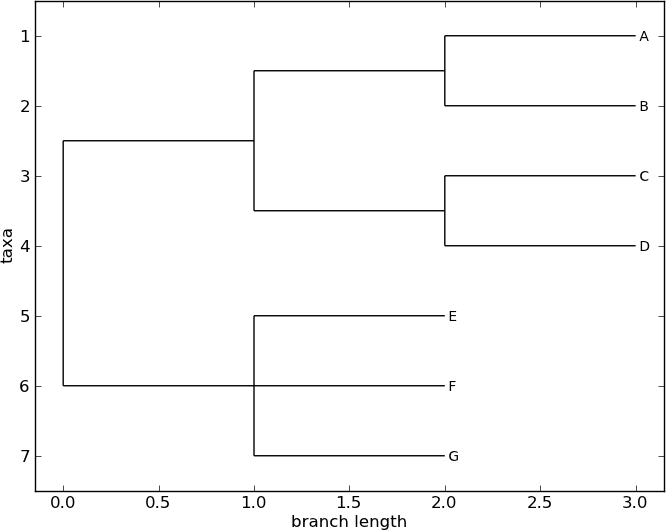
\includegraphics{phylo-simple-draw.png}


\subsection{13.1.1  给树的分支上颜色}
\label{chr13:id2}
函数 \code{draw} 和 \code{draw\_graphviz} 支持在树中显示不同的颜色和分支宽度。
从Biopython 1.59开始,Clade对象就开始支持 \code{color} 和 \code{width} 属性,
且使用他们不需要额外支持。这两个属性都表示导向给定的进化枝前面的分支的
属性,并依次往下作用,所以所有的后代分支在显示时也都继承相同的宽度和颜
色。

在早期的Biopython版本中,PhyloXML树有些特殊的特性,使用这些属性需要首先
将这个树转换为一个基本树对象的子类Phylogeny,该类在Bio.Phylo.PhyloXML模
块中。

在Biopython 1.55和之后的版本中,这是一个很方便的树方法:
\DUspan{operator}{}\DUspan{name}{}\DUspan{operator}{}\DUspan{name}{}\DUspan{operator}{}\DUspan{name}{}\DUspan{punctuation}{}
\begin{Verbatim}[commandchars=\\\{\}]
\PYG{g+gp}{\PYGZgt{}\PYGZgt{}\PYGZgt{} }\PYG{n}{tree} \PYG{o}{=} \PYG{n}{tree}\PYG{o}{.}\PYG{n}{as\PYGZus{}phyloxml}\PYG{p}{(}\PYG{p}{)}
\end{Verbatim}

在Biopython 1.54中, 你能通过导入一个额外的模块实现相同的事情:
\DUspan{operator}{}\DUspan{keyword,namespace}{}\DUspan{name,namespace}{}\DUspan{keyword,namespace}{}\DUspan{name}{}\DUspan{operator}{}\DUspan{name}{}\DUspan{operator}{}\DUspan{name}{}\DUspan{operator}{}\DUspan{name}{}\DUspan{punctuation}{}\DUspan{name}{}\DUspan{punctuation}{}
\begin{Verbatim}[commandchars=\\\{\}]
\PYG{g+gp}{\PYGZgt{}\PYGZgt{}\PYGZgt{} }\PYG{k+kn}{from} \PYG{n+nn}{Bio.Phylo.PhyloXML} \PYG{k+kn}{import} \PYG{n}{Phylogeny}
\PYG{g+gp}{\PYGZgt{}\PYGZgt{}\PYGZgt{} }\PYG{n}{tree} \PYG{o}{=} \PYG{n}{Phylogeny}\PYG{o}{.}\PYG{n}{from\PYGZus{}tree}\PYG{p}{(}\PYG{n}{tree}\PYG{p}{)}
\end{Verbatim}

注意Newick和Nexus文件类型并不支持分支颜色和宽度,如果你在Bio.Phylo中使用
这些属性,你只能保存这些值到PhyloXML格式中。(你也可以保存成Newick或Nexus
格式,但是颜色和宽度信息在输出的文件时会被忽略掉。)

现在我们开始指定颜色。首先,我们将设置根进化枝为灰色。我们能通过赋值24位
的颜色值来实现,用三位数的RGB值、HTML格式的十六进制字符串、或者预先设置好的
颜色名称。
\DUspan{operator}{}\DUspan{name}{}\DUspan{operator}{}\DUspan{name}{}\DUspan{operator}{}\DUspan{name}{}\DUspan{operator}{}\DUspan{punctuation}{}\DUspan{literal,number,integer}{}\DUspan{punctuation}{}\DUspan{literal,number,integer}{}\DUspan{punctuation}{}\DUspan{literal,number,integer}{}\DUspan{punctuation}{}
\begin{Verbatim}[commandchars=\\\{\}]
\PYG{g+gp}{\PYGZgt{}\PYGZgt{}\PYGZgt{} }\PYG{n}{tree}\PYG{o}{.}\PYG{n}{root}\PYG{o}{.}\PYG{n}{color} \PYG{o}{=} \PYG{p}{(}\PYG{l+m+mi}{128}\PYG{p}{,} \PYG{l+m+mi}{128}\PYG{p}{,} \PYG{l+m+mi}{128}\PYG{p}{)}
\end{Verbatim}

Or:
\DUspan{operator}{}\DUspan{name}{}\DUspan{operator}{}\DUspan{name}{}\DUspan{operator}{}\DUspan{name}{}\DUspan{operator}{}\DUspan{literal,string}{}
\begin{Verbatim}[commandchars=\\\{\}]
\PYG{g+gp}{\PYGZgt{}\PYGZgt{}\PYGZgt{} }\PYG{n}{tree}\PYG{o}{.}\PYG{n}{root}\PYG{o}{.}\PYG{n}{color} \PYG{o}{=} \PYG{l+s}{\PYGZdq{}}\PYG{l+s}{\PYGZsh{}808080}\PYG{l+s}{\PYGZdq{}}
\end{Verbatim}

Or:
\DUspan{operator}{}\DUspan{name}{}\DUspan{operator}{}\DUspan{name}{}\DUspan{operator}{}\DUspan{name}{}\DUspan{operator}{}\DUspan{literal,string}{}
\begin{Verbatim}[commandchars=\\\{\}]
\PYG{g+gp}{\PYGZgt{}\PYGZgt{}\PYGZgt{} }\PYG{n}{tree}\PYG{o}{.}\PYG{n}{root}\PYG{o}{.}\PYG{n}{color} \PYG{o}{=} \PYG{l+s}{\PYGZdq{}}\PYG{l+s}{gray}\PYG{l+s}{\PYGZdq{}}
\end{Verbatim}

一个进化枝的颜色会被当作从上而下整个进化枝的颜色,所以我们这里设置根的
的颜色会将整个树的颜色变为灰色。我们能通过在树中下面分支赋值不同的颜色
来重新定义某个分支的颜色。

让我们先定位“E”和“F”最近祖先(MRCA)节点。方法 \code{common\_ancestor} 返回
原始树中这个进化枝的引用,所以当我们设置该进化枝为“salmon”颜色时,这个颜
色则会在原始的树中显示出来。
\DUspan{operator}{}\DUspan{name}{}\DUspan{operator}{}\DUspan{name}{}\DUspan{operator}{}\DUspan{name}{}\DUspan{punctuation}{}\DUspan{literal,string}{}\DUspan{punctuation}{}\DUspan{literal,string}{}\DUspan{punctuation}{}\DUspan{punctuation}{}\DUspan{literal,string}{}\DUspan{punctuation}{}\DUspan{literal,string}{}\DUspan{punctuation}{}\DUspan{operator}{}\DUspan{name}{}\DUspan{operator}{}\DUspan{name}{}\DUspan{operator}{}\DUspan{literal,string}{}
\begin{Verbatim}[commandchars=\\\{\}]
\PYG{g+gp}{\PYGZgt{}\PYGZgt{}\PYGZgt{} }\PYG{n}{mrca} \PYG{o}{=} \PYG{n}{tree}\PYG{o}{.}\PYG{n}{common\PYGZus{}ancestor}\PYG{p}{(}\PYG{p}{\PYGZob{}}\PYG{l+s}{\PYGZdq{}}\PYG{l+s}{name}\PYG{l+s}{\PYGZdq{}}\PYG{p}{:} \PYG{l+s}{\PYGZdq{}}\PYG{l+s}{E}\PYG{l+s}{\PYGZdq{}}\PYG{p}{\PYGZcb{}}\PYG{p}{,} \PYG{p}{\PYGZob{}}\PYG{l+s}{\PYGZdq{}}\PYG{l+s}{name}\PYG{l+s}{\PYGZdq{}}\PYG{p}{:} \PYG{l+s}{\PYGZdq{}}\PYG{l+s}{F}\PYG{l+s}{\PYGZdq{}}\PYG{p}{\PYGZcb{}}\PYG{p}{)}
\PYG{g+gp}{\PYGZgt{}\PYGZgt{}\PYGZgt{} }\PYG{n}{mrca}\PYG{o}{.}\PYG{n}{color} \PYG{o}{=} \PYG{l+s}{\PYGZdq{}}\PYG{l+s}{salmon}\PYG{l+s}{\PYGZdq{}}
\end{Verbatim}

当我们碰巧明确地知道某个进化枝在树中的位置,以嵌套列表的形式,我们就能
通过索引的方式直接跳到那个位置。这里,索引 \code{{[}0,1{]}} 表示根节点的第一个
子代节点的第二个子代。
\DUspan{operator}{}\DUspan{name}{}\DUspan{operator}{}\DUspan{name}{}\DUspan{punctuation}{}\DUspan{literal,number,integer}{}\DUspan{punctuation}{}\DUspan{literal,number,integer}{}\DUspan{punctuation}{}\DUspan{operator}{}\DUspan{name}{}\DUspan{operator}{}\DUspan{literal,string}{}
\begin{Verbatim}[commandchars=\\\{\}]
\PYG{g+gp}{\PYGZgt{}\PYGZgt{}\PYGZgt{} }\PYG{n}{tree}\PYG{o}{.}\PYG{n}{clade}\PYG{p}{[}\PYG{l+m+mi}{0}\PYG{p}{,}\PYG{l+m+mi}{1}\PYG{p}{]}\PYG{o}{.}\PYG{n}{color} \PYG{o}{=} \PYG{l+s}{\PYGZdq{}}\PYG{l+s}{blue}\PYG{l+s}{\PYGZdq{}}
\end{Verbatim}

最后,展示一下我们的工作结果 (见 Fig. {\hyperref[chr13:fig-phylo-color-draw]{\emph{13.1.1}}} ):
\DUspan{operator}{}\DUspan{name}{}\DUspan{operator}{}\DUspan{name}{}\DUspan{punctuation}{}\DUspan{name}{}\DUspan{punctuation}{}
\begin{Verbatim}[commandchars=\\\{\}]
\PYG{g+gp}{\PYGZgt{}\PYGZgt{}\PYGZgt{} }\PYG{n}{Phylo}\PYG{o}{.}\PYG{n}{draw}\PYG{p}{(}\PYG{n}{tree}\PYG{p}{)}
\end{Verbatim}
\phantomsection\label{chr13:fig-phylo-color-draw}
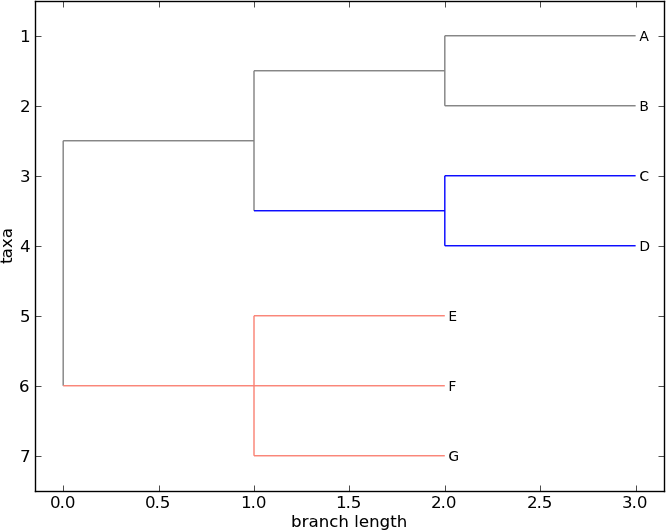
\includegraphics{phylo-color-draw.png}

注意进化枝的颜色包括导向它的分支和它的子代的分支。E和F的共同祖先结果刚好
在根分支下面,而通过这样上色,我们能清楚的看出这个树的根在哪里。

我们已经完成了很多!现在让我们休息一下,保存一下我们的工作。使用一个文件
名或句柄(这里我们使用标准输出来查看将会输出什么)和 \code{phyloxml} 格式来
调用 \code{write} 函数。PhyloXML格式保存了我们设置的颜色,所以你能通过其他树
查看工具,如Archaeopteryx,打开这个phyloXML文件,这些颜色也会显示出来。
\DUspan{operator}{}\DUspan{keyword,namespace}{}\DUspan{name,namespace}{}\DUspan{operator}{}\DUspan{name}{}\DUspan{operator}{}\DUspan{name}{}\DUspan{punctuation}{}\DUspan{name}{}\DUspan{punctuation}{}\DUspan{name}{}\DUspan{operator}{}\DUspan{name}{}\DUspan{punctuation}{}\DUspan{literal,string}{}\DUspan{punctuation}{}\DUspan{operator}{}\DUspan{name}{}\DUspan{punctuation}{}\DUspan{name}{}\DUspan{name}{}\DUspan{punctuation}{}\DUspan{name}{}\DUspan{operator}{}\DUspan{literal,string}{}\DUspan{operator}{}\DUspan{operator}{}\DUspan{name}{}\DUspan{punctuation}{}\DUspan{name}{}\DUspan{name}{}\DUspan{operator}{}\DUspan{literal,string}{}\DUspan{operator}{}\DUspan{operator}{}\DUspan{name}{}\DUspan{punctuation}{}\DUspan{name}{}\DUspan{operator}{}\DUspan{operator}{}\DUspan{name}{}\DUspan{punctuation}{}\DUspan{name}{}\DUspan{operator}{}\DUspan{literal,number,float}{}\DUspan{operator}{}\DUspan{name}{}\DUspan{punctuation}{}\DUspan{name}{}\DUspan{operator}{}\DUspan{operator}{}\DUspan{name}{}\DUspan{punctuation}{}\DUspan{name}{}\DUspan{operator}{}\DUspan{operator}{}\DUspan{name}{}\DUspan{punctuation}{}\DUspan{name}{}\DUspan{operator}{}\DUspan{literal,number,integer}{}\DUspan{operator}{}\DUspan{name}{}\DUspan{punctuation}{}\DUspan{name}{}\DUspan{operator}{}\DUspan{operator}{}\DUspan{name}{}\DUspan{punctuation}{}\DUspan{name}{}\DUspan{operator}{}\DUspan{literal,number,integer}{}\DUspan{operator}{}\DUspan{name}{}\DUspan{punctuation}{}\DUspan{name}{}\DUspan{operator}{}\DUspan{operator}{}\DUspan{name}{}\DUspan{punctuation}{}\DUspan{name}{}\DUspan{operator}{}\DUspan{literal,number,integer}{}\DUspan{operator}{}\DUspan{name}{}\DUspan{punctuation}{}\DUspan{name}{}\DUspan{operator}{}\DUspan{operator}{}\DUspan{name}{}\DUspan{punctuation}{}\DUspan{name}{}\DUspan{operator}{}\DUspan{operator}{}\DUspan{name}{}\DUspan{punctuation}{}\DUspan{name}{}\DUspan{operator}{}\DUspan{operator}{}\DUspan{name}{}\DUspan{punctuation}{}\DUspan{name}{}\DUspan{operator}{}\DUspan{literal,number,float}{}\DUspan{operator}{}\DUspan{name}{}\DUspan{punctuation}{}\DUspan{name}{}\DUspan{operator}{}\DUspan{operator}{}\DUspan{name}{}\DUspan{punctuation}{}\DUspan{name}{}\DUspan{operator}{}\DUspan{operator}{}\DUspan{name}{}\DUspan{punctuation}{}\DUspan{name}{}\DUspan{operator}{}\DUspan{literal,number,float}{}\DUspan{operator}{}\DUspan{name}{}\DUspan{punctuation}{}\DUspan{name}{}\DUspan{operator}{}\DUspan{operator}{}\DUspan{name}{}\DUspan{punctuation}{}\DUspan{name}{}\DUspan{operator}{}\DUspan{operator}{}\DUspan{name}{}\DUspan{punctuation}{}\DUspan{name}{}\DUspan{operator}{}\DUspan{name}{}\DUspan{operator}{}\DUspan{name}{}\DUspan{punctuation}{}\DUspan{name}{}\DUspan{operator}{}\DUspan{operator}{}
\begin{Verbatim}[commandchars=\\\{\}]
\PYG{g+gp}{\PYGZgt{}\PYGZgt{}\PYGZgt{} }\PYG{k+kn}{import} \PYG{n+nn}{sys}
\PYG{g+gp}{\PYGZgt{}\PYGZgt{}\PYGZgt{} }\PYG{n}{Phylo}\PYG{o}{.}\PYG{n}{write}\PYG{p}{(}\PYG{n}{tree}\PYG{p}{,} \PYG{n}{sys}\PYG{o}{.}\PYG{n}{stdout}\PYG{p}{,} \PYG{l+s}{\PYGZdq{}}\PYG{l+s}{phyloxml}\PYG{l+s}{\PYGZdq{}}\PYG{p}{)}

\PYG{g+go}{\PYGZlt{}phy:phyloxml xmlns:phy=\PYGZdq{}http://www.phyloxml.org\PYGZdq{}\PYGZgt{}}
\PYG{g+go}{  \PYGZlt{}phy:phylogeny rooted=\PYGZdq{}true\PYGZdq{}\PYGZgt{}}
\PYG{g+go}{    \PYGZlt{}phy:clade\PYGZgt{}}
\PYG{g+go}{      \PYGZlt{}phy:branch\PYGZus{}length\PYGZgt{}1.0\PYGZlt{}/phy:branch\PYGZus{}length\PYGZgt{}}
\PYG{g+go}{      \PYGZlt{}phy:color\PYGZgt{}}
\PYG{g+go}{        \PYGZlt{}phy:red\PYGZgt{}128\PYGZlt{}/phy:red\PYGZgt{}}
\PYG{g+go}{        \PYGZlt{}phy:green\PYGZgt{}128\PYGZlt{}/phy:green\PYGZgt{}}
\PYG{g+go}{        \PYGZlt{}phy:blue\PYGZgt{}128\PYGZlt{}/phy:blue\PYGZgt{}}
\PYG{g+go}{      \PYGZlt{}/phy:color\PYGZgt{}}
\PYG{g+go}{      \PYGZlt{}phy:clade\PYGZgt{}}
\PYG{g+go}{        \PYGZlt{}phy:branch\PYGZus{}length\PYGZgt{}1.0\PYGZlt{}/phy:branch\PYGZus{}length\PYGZgt{}}
\PYG{g+go}{        \PYGZlt{}phy:clade\PYGZgt{}}
\PYG{g+go}{          \PYGZlt{}phy:branch\PYGZus{}length\PYGZgt{}1.0\PYGZlt{}/phy:branch\PYGZus{}length\PYGZgt{}}
\PYG{g+go}{          \PYGZlt{}phy:clade\PYGZgt{}}
\PYG{g+go}{            \PYGZlt{}phy:name\PYGZgt{}A\PYGZlt{}/phy:name\PYGZgt{}}
\PYG{g+go}{            ...}
\end{Verbatim}

本章的其余部分将更加细致的介绍Bio.Phylo核心功能。关于Bio.Phylo的更多例
子,请参见Biopython.org上的Cookbook手册页面。

\href{http://biopython.org/wiki/Phylo\_cookbook}{http://biopython.org/wiki/Phylo\_cookbook}


\section{13.2  I/O 函数}
\label{chr13:i-o}
和SeqIO、AlignIO类似, Phylo使用四个函数处理文件的输入输出: \code{parse} 、
\code{read} 、 \code{write} 和 \code{convert} ,所有的函数都支持Newick、NEXUS、
phyloXML和NeXML等树文件格式。

\code{read} 函数解析并返回给定文件中的单个树。注意,如果文件中包含多个或不包含任何树,它将抛出一个错误。
\DUspan{operator}{}\DUspan{keyword,namespace}{}\DUspan{name,namespace}{}\DUspan{keyword,namespace}{}\DUspan{name}{}\DUspan{operator}{}\DUspan{name}{}\DUspan{operator}{}\DUspan{name}{}\DUspan{operator}{}\DUspan{name}{}\DUspan{punctuation}{}\DUspan{literal,string}{}\DUspan{punctuation}{}\DUspan{literal,string}{}\DUspan{punctuation}{}\DUspan{operator}{}\DUspan{keyword}{}\DUspan{name}{}
\begin{Verbatim}[commandchars=\\\{\}]
\PYG{g+gp}{\PYGZgt{}\PYGZgt{}\PYGZgt{} }\PYG{k+kn}{from} \PYG{n+nn}{Bio} \PYG{k+kn}{import} \PYG{n}{Phylo}
\PYG{g+gp}{\PYGZgt{}\PYGZgt{}\PYGZgt{} }\PYG{n}{tree} \PYG{o}{=} \PYG{n}{Phylo}\PYG{o}{.}\PYG{n}{read}\PYG{p}{(}\PYG{l+s}{\PYGZdq{}}\PYG{l+s}{Tests/Nexus/int\PYGZus{}node\PYGZus{}labels.nwk}\PYG{l+s}{\PYGZdq{}}\PYG{p}{,} \PYG{l+s}{\PYGZdq{}}\PYG{l+s}{newick}\PYG{l+s}{\PYGZdq{}}\PYG{p}{)}
\PYG{g+gp}{\PYGZgt{}\PYGZgt{}\PYGZgt{} }\PYG{k}{print} \PYG{n}{tree}
\end{Verbatim}

(Biopython发布包的 \code{Tests/Nexus/} 和 \code{Tests/PhyloXML/} 文件夹中有相应的例子)

处理多个(或者未知个数)的树文件,需要使用 \code{parse} 函数迭代给定文件中的每一个树。
\DUspan{operator}{}\DUspan{name}{}\DUspan{operator}{}\DUspan{name}{}\DUspan{operator}{}\DUspan{name}{}\DUspan{punctuation}{}\DUspan{literal,string}{}\DUspan{punctuation}{}\DUspan{literal,string}{}\DUspan{punctuation}{}\DUspan{operator}{}\DUspan{keyword}{}\DUspan{name}{}\DUspan{operator,word}{}\DUspan{name}{}\DUspan{punctuation}{}\DUspan{operator}{}\DUspan{keyword}{}\DUspan{name}{}
\begin{Verbatim}[commandchars=\\\{\}]
\PYG{g+gp}{\PYGZgt{}\PYGZgt{}\PYGZgt{} }\PYG{n}{trees} \PYG{o}{=} \PYG{n}{Phylo}\PYG{o}{.}\PYG{n}{parse}\PYG{p}{(}\PYG{l+s}{\PYGZdq{}}\PYG{l+s}{Tests/PhyloXML/phyloxml\PYGZus{}examples.xml}\PYG{l+s}{\PYGZdq{}}\PYG{p}{,} \PYG{l+s}{\PYGZdq{}}\PYG{l+s}{phyloxml}\PYG{l+s}{\PYGZdq{}}\PYG{p}{)}
\PYG{g+gp}{\PYGZgt{}\PYGZgt{}\PYGZgt{} }\PYG{k}{for} \PYG{n}{tree} \PYG{o+ow}{in} \PYG{n}{trees}\PYG{p}{:}
\PYG{g+gp}{... }    \PYG{k}{print} \PYG{n}{tree}
\end{Verbatim}

使用 \code{write} 函数输出一个或多个可迭代的树。
\DUspan{operator}{}\DUspan{name}{}\DUspan{operator}{}\DUspan{name,builtin}{}\DUspan{punctuation}{}\DUspan{name}{}\DUspan{operator}{}\DUspan{name}{}\DUspan{punctuation}{}\DUspan{literal,string}{}\DUspan{punctuation}{}\DUspan{literal,string}{}\DUspan{punctuation}{}\DUspan{operator}{}\DUspan{name}{}\DUspan{operator}{}\DUspan{name}{}\DUspan{punctuation}{}\DUspan{literal,number,integer}{}\DUspan{punctuation}{}\DUspan{operator}{}\DUspan{name}{}\DUspan{operator}{}\DUspan{name}{}\DUspan{punctuation}{}\DUspan{literal,number,integer}{}\DUspan{punctuation}{}\DUspan{operator}{}\DUspan{name}{}\DUspan{operator}{}\DUspan{name}{}\DUspan{punctuation}{}\DUspan{name}{}\DUspan{punctuation}{}\DUspan{literal,string}{}\DUspan{punctuation}{}\DUspan{literal,string}{}\DUspan{punctuation}{}\DUspan{literal,number,integer}{}\DUspan{operator}{}\DUspan{name}{}\DUspan{operator}{}\DUspan{name}{}\DUspan{punctuation}{}\DUspan{name}{}\DUspan{punctuation}{}\DUspan{literal,string}{}\DUspan{punctuation}{}\DUspan{literal,string}{}\DUspan{punctuation}{}\DUspan{literal,number,integer}{}
\begin{Verbatim}[commandchars=\\\{\}]
\PYG{g+gp}{\PYGZgt{}\PYGZgt{}\PYGZgt{} }\PYG{n}{trees} \PYG{o}{=} \PYG{n+nb}{list}\PYG{p}{(}\PYG{n}{Phylo}\PYG{o}{.}\PYG{n}{parse}\PYG{p}{(}\PYG{l+s}{\PYGZdq{}}\PYG{l+s}{phyloxml\PYGZus{}examples.xml}\PYG{l+s}{\PYGZdq{}}\PYG{p}{,} \PYG{l+s}{\PYGZdq{}}\PYG{l+s}{phyloxml}\PYG{l+s}{\PYGZdq{}}\PYG{p}{)}\PYG{p}{)}
\PYG{g+gp}{\PYGZgt{}\PYGZgt{}\PYGZgt{} }\PYG{n}{tree1} \PYG{o}{=} \PYG{n}{trees}\PYG{p}{[}\PYG{l+m+mi}{0}\PYG{p}{]}
\PYG{g+gp}{\PYGZgt{}\PYGZgt{}\PYGZgt{} }\PYG{n}{others} \PYG{o}{=} \PYG{n}{trees}\PYG{p}{[}\PYG{l+m+mi}{1}\PYG{p}{:}\PYG{p}{]}
\PYG{g+gp}{\PYGZgt{}\PYGZgt{}\PYGZgt{} }\PYG{n}{Phylo}\PYG{o}{.}\PYG{n}{write}\PYG{p}{(}\PYG{n}{tree1}\PYG{p}{,} \PYG{l+s}{\PYGZdq{}}\PYG{l+s}{tree1.xml}\PYG{l+s}{\PYGZdq{}}\PYG{p}{,} \PYG{l+s}{\PYGZdq{}}\PYG{l+s}{phyloxml}\PYG{l+s}{\PYGZdq{}}\PYG{p}{)}
\PYG{g+go}{1}
\PYG{g+gp}{\PYGZgt{}\PYGZgt{}\PYGZgt{} }\PYG{n}{Phylo}\PYG{o}{.}\PYG{n}{write}\PYG{p}{(}\PYG{n}{others}\PYG{p}{,} \PYG{l+s}{\PYGZdq{}}\PYG{l+s}{other\PYGZus{}trees.xml}\PYG{l+s}{\PYGZdq{}}\PYG{p}{,} \PYG{l+s}{\PYGZdq{}}\PYG{l+s}{phyloxml}\PYG{l+s}{\PYGZdq{}}\PYG{p}{)}
\PYG{g+go}{12}
\end{Verbatim}

使用 \code{convert} 函数转换任何支持的树格式。
\DUspan{operator}{}\DUspan{name}{}\DUspan{operator}{}\DUspan{name}{}\DUspan{punctuation}{}\DUspan{literal,string}{}\DUspan{punctuation}{}\DUspan{literal,string}{}\DUspan{punctuation}{}\DUspan{literal,string}{}\DUspan{punctuation}{}\DUspan{literal,string}{}\DUspan{punctuation}{}\DUspan{literal,number,integer}{}\DUspan{operator}{}\DUspan{name}{}\DUspan{operator}{}\DUspan{name}{}\DUspan{punctuation}{}\DUspan{literal,string}{}\DUspan{punctuation}{}\DUspan{literal,string}{}\DUspan{punctuation}{}\DUspan{literal,string}{}\DUspan{punctuation}{}\DUspan{literal,string}{}\DUspan{literal,number,integer}{}
\begin{Verbatim}[commandchars=\\\{\}]
\PYG{g+gp}{\PYGZgt{}\PYGZgt{}\PYGZgt{} }\PYG{n}{Phylo}\PYG{o}{.}\PYG{n}{convert}\PYG{p}{(}\PYG{l+s}{\PYGZdq{}}\PYG{l+s}{tree1.dnd}\PYG{l+s}{\PYGZdq{}}\PYG{p}{,} \PYG{l+s}{\PYGZdq{}}\PYG{l+s}{newick}\PYG{l+s}{\PYGZdq{}}\PYG{p}{,} \PYG{l+s}{\PYGZdq{}}\PYG{l+s}{tree1.xml}\PYG{l+s}{\PYGZdq{}}\PYG{p}{,} \PYG{l+s}{\PYGZdq{}}\PYG{l+s}{nexml}\PYG{l+s}{\PYGZdq{}}\PYG{p}{)}
\PYG{g+go}{1}
\PYG{g+gp}{\PYGZgt{}\PYGZgt{}\PYGZgt{} }\PYG{n}{Phylo}\PYG{o}{.}\PYG{n}{convert}\PYG{p}{(}\PYG{l+s}{\PYGZdq{}}\PYG{l+s}{other\PYGZus{}trees.xml}\PYG{l+s}{\PYGZdq{}}\PYG{p}{,} \PYG{l+s}{\PYGZdq{}}\PYG{l+s}{phyloxml}\PYG{l+s}{\PYGZdq{}}\PYG{p}{,} \PYG{l+s}{\PYGZdq{}}\PYG{l+s}{other\PYGZus{}trees.nex}\PYG{l+s}{\PYGZdq{}}\PYG{p}{,} \PYG{l+s}{\PYGZsq{}}\PYG{l+s}{nexus}\PYG{l+s}{\PYGZdq{}}\PYG{l+s}{)}
\PYG{g+go}{12}
\end{Verbatim}

和SeqIO和AlignIO类似,当使用字符串而不是文件作为输入输出时,需要使用 ‵‵StringIO{}`{}` 函数。
\DUspan{operator}{}\DUspan{keyword,namespace}{}\DUspan{name,namespace}{}\DUspan{keyword,namespace}{}\DUspan{name}{}\DUspan{operator}{}\DUspan{keyword,namespace}{}\DUspan{name,namespace}{}\DUspan{keyword,namespace}{}\DUspan{name}{}\DUspan{operator}{}\DUspan{name}{}\DUspan{operator}{}\DUspan{name}{}\DUspan{punctuation}{}\DUspan{literal,string}{}\DUspan{punctuation}{}\DUspan{operator}{}\DUspan{name}{}\DUspan{operator}{}\DUspan{name}{}\DUspan{operator}{}\DUspan{name}{}\DUspan{punctuation}{}\DUspan{name}{}\DUspan{punctuation}{}\DUspan{literal,string}{}\DUspan{punctuation}{}
\begin{Verbatim}[commandchars=\\\{\}]
\PYG{g+gp}{\PYGZgt{}\PYGZgt{}\PYGZgt{} }\PYG{k+kn}{from} \PYG{n+nn}{Bio} \PYG{k+kn}{import} \PYG{n}{Phylo}
\PYG{g+gp}{\PYGZgt{}\PYGZgt{}\PYGZgt{} }\PYG{k+kn}{from} \PYG{n+nn}{StringIO} \PYG{k+kn}{import} \PYG{n}{StringIO}
\PYG{g+gp}{\PYGZgt{}\PYGZgt{}\PYGZgt{} }\PYG{n}{handle} \PYG{o}{=} \PYG{n}{StringIO}\PYG{p}{(}\PYG{l+s}{\PYGZdq{}}\PYG{l+s}{(((A,B),(C,D)),(E,F,G));}\PYG{l+s}{\PYGZdq{}}\PYG{p}{)}
\PYG{g+gp}{\PYGZgt{}\PYGZgt{}\PYGZgt{} }\PYG{n}{tree} \PYG{o}{=} \PYG{n}{Phylo}\PYG{o}{.}\PYG{n}{read}\PYG{p}{(}\PYG{n}{handle}\PYG{p}{,} \PYG{l+s}{\PYGZdq{}}\PYG{l+s}{newick}\PYG{l+s}{\PYGZdq{}}\PYG{p}{)}
\end{Verbatim}


\section{13.3  查看和导出树}
\label{chr13:id3}
了解一个 \code{Tree} 对象概况的最简单的方法是用 \code{print} 函数将它打印出来:
\DUspan{operator}{}\DUspan{name}{}\DUspan{operator}{}\DUspan{name}{}\DUspan{operator}{}\DUspan{name}{}\DUspan{punctuation}{}\DUspan{literal,string}{}\DUspan{punctuation}{}\DUspan{literal,string}{}\DUspan{punctuation}{}\DUspan{operator}{}\DUspan{keyword}{}\DUspan{name}{}\DUspan{name}{}\DUspan{punctuation}{}\DUspan{name}{}\DUspan{operator}{}\DUspan{literal,string}{}\DUspan{punctuation}{}\DUspan{name}{}\DUspan{operator}{}\DUspan{literal,string}{}\DUspan{name}{}\DUspan{operator}{}\DUspan{literal,string}{}\DUspan{name}{}\DUspan{keyword,namespace}{}\DUspan{name,namespace}{}\DUspan{name,namespace}{}\DUspan{name,namespace}{}\DUspan{literal,string}{}\DUspan{punctuation}{}\DUspan{name}{}\DUspan{punctuation}{}\DUspan{name}{}\DUspan{punctuation}{}\DUspan{name}{}\DUspan{operator}{}\DUspan{literal,string}{}\DUspan{punctuation}{}\DUspan{name}{}\DUspan{punctuation}{}\DUspan{name}{}\DUspan{operator}{}\DUspan{literal,string}{}\DUspan{punctuation}{}\DUspan{name}{}\DUspan{operator}{}\DUspan{literal,string}{}\DUspan{punctuation}{}\DUspan{name}{}\DUspan{punctuation}{}\DUspan{name}{}\DUspan{operator}{}\DUspan{literal,string}{}\DUspan{punctuation}{}\DUspan{name}{}\DUspan{operator}{}\DUspan{literal,string}{}\DUspan{punctuation}{}\DUspan{name}{}\DUspan{punctuation}{}\DUspan{name}{}\DUspan{operator}{}\DUspan{literal,string}{}\DUspan{punctuation}{}\DUspan{name}{}\DUspan{operator}{}\DUspan{literal,string}{}\DUspan{punctuation}{}
\begin{Verbatim}[commandchars=\\\{\}]
\PYG{g+gp}{\PYGZgt{}\PYGZgt{}\PYGZgt{} }\PYG{n}{tree} \PYG{o}{=} \PYG{n}{Phylo}\PYG{o}{.}\PYG{n}{read}\PYG{p}{(}\PYG{l+s}{\PYGZdq{}}\PYG{l+s}{Tests/PhyloXML/example.xml}\PYG{l+s}{\PYGZdq{}}\PYG{p}{,} \PYG{l+s}{\PYGZdq{}}\PYG{l+s}{phyloxml}\PYG{l+s}{\PYGZdq{}}\PYG{p}{)}
\PYG{g+gp}{\PYGZgt{}\PYGZgt{}\PYGZgt{} }\PYG{k}{print} \PYG{n}{tree}
\PYG{g+go}{Phylogeny(rooted=\PYGZsq{}True\PYGZsq{}, description=\PYGZsq{}phyloXML allows to use either a \PYGZdq{}branch\PYGZus{}length\PYGZdq{}}
\PYG{g+go}{attribute...\PYGZsq{}, name=\PYGZsq{}example from Prof. Joe Felsenstein\PYGZsq{}s book \PYGZdq{}Inferring Phyl...\PYGZsq{})}
\PYG{g+go}{    Clade()}
\PYG{g+go}{        Clade(branch\PYGZus{}length=\PYGZsq{}0.06\PYGZsq{})}
\PYG{g+go}{            Clade(branch\PYGZus{}length=\PYGZsq{}0.102\PYGZsq{}, name=\PYGZsq{}A\PYGZsq{})}
\PYG{g+go}{            Clade(branch\PYGZus{}length=\PYGZsq{}0.23\PYGZsq{}, name=\PYGZsq{}B\PYGZsq{})}
\PYG{g+go}{        Clade(branch\PYGZus{}length=\PYGZsq{}0.4\PYGZsq{}, name=\PYGZsq{}C\PYGZsq{})}
\end{Verbatim}

上面实际上是Biopython的树对象层次结构的一个概况。然而更可能的情况是,你希望见到
画出树的形状,这里有三个函数来做这件事情。

如我们在demo中看到的一样, \code{draw\_ascii} 打印一个树的ascii-art图像(有根进化树)
到标准输出,或者一个打开的文件句柄,若有提供。不是所有关于树的信息被显示出来,但是它提供了一个
不依靠于任何外部依赖的快速查看树的方法。
\DUspan{operator}{}\DUspan{name}{}\DUspan{operator}{}\DUspan{name}{}\DUspan{operator}{}\DUspan{name}{}\DUspan{punctuation}{}\DUspan{literal,string}{}\DUspan{punctuation}{}\DUspan{literal,string}{}\DUspan{punctuation}{}\DUspan{operator}{}\DUspan{name}{}\DUspan{operator}{}\DUspan{name}{}\DUspan{punctuation}{}\DUspan{name}{}\DUspan{punctuation}{}\DUspan{name}{}\DUspan{name}{}\DUspan{name}{}\DUspan{operator}{}\DUspan{name}{}\DUspan{operator}{}\DUspan{operator}{}\DUspan{name}{}\DUspan{name}{}\DUspan{operator}{}\DUspan{operator}{}\DUspan{name}{}\DUspan{name}{}
\begin{Verbatim}[commandchars=\\\{\}]
\PYG{g+gp}{\PYGZgt{}\PYGZgt{}\PYGZgt{} }\PYG{n}{tree} \PYG{o}{=} \PYG{n}{Phylo}\PYG{o}{.}\PYG{n}{read}\PYG{p}{(}\PYG{l+s}{\PYGZdq{}}\PYG{l+s}{example.xml}\PYG{l+s}{\PYGZdq{}}\PYG{p}{,} \PYG{l+s}{\PYGZdq{}}\PYG{l+s}{phyloxml}\PYG{l+s}{\PYGZdq{}}\PYG{p}{)}
\PYG{g+gp}{\PYGZgt{}\PYGZgt{}\PYGZgt{} }\PYG{n}{Phylo}\PYG{o}{.}\PYG{n}{draw\PYGZus{}ascii}\PYG{p}{(}\PYG{n}{tree}\PYG{p}{)}
\PYG{g+go}{             \PYGZus{}\PYGZus{}\PYGZus{}\PYGZus{}\PYGZus{}\PYGZus{}\PYGZus{}\PYGZus{}\PYGZus{}\PYGZus{}\PYGZus{}\PYGZus{}\PYGZus{}\PYGZus{}\PYGZus{}\PYGZus{}\PYGZus{}\PYGZus{} A}
\PYG{g+go}{  \PYGZus{}\PYGZus{}\PYGZus{}\PYGZus{}\PYGZus{}\PYGZus{}\PYGZus{}\PYGZus{}\PYGZus{}\PYGZus{}\textbar{}}
\PYG{g+go}{\PYGZus{}\textbar{}          \textbar{}\PYGZus{}\PYGZus{}\PYGZus{}\PYGZus{}\PYGZus{}\PYGZus{}\PYGZus{}\PYGZus{}\PYGZus{}\PYGZus{}\PYGZus{}\PYGZus{}\PYGZus{}\PYGZus{}\PYGZus{}\PYGZus{}\PYGZus{}\PYGZus{}\PYGZus{}\PYGZus{}\PYGZus{}\PYGZus{}\PYGZus{}\PYGZus{}\PYGZus{}\PYGZus{}\PYGZus{}\PYGZus{}\PYGZus{}\PYGZus{}\PYGZus{}\PYGZus{}\PYGZus{}\PYGZus{}\PYGZus{}\PYGZus{}\PYGZus{}\PYGZus{}\PYGZus{}\PYGZus{}\PYGZus{}\PYGZus{}\PYGZus{} B}
\PYG{g+go}{ \textbar{}}
\PYG{g+go}{ \textbar{}\PYGZus{}\PYGZus{}\PYGZus{}\PYGZus{}\PYGZus{}\PYGZus{}\PYGZus{}\PYGZus{}\PYGZus{}\PYGZus{}\PYGZus{}\PYGZus{}\PYGZus{}\PYGZus{}\PYGZus{}\PYGZus{}\PYGZus{}\PYGZus{}\PYGZus{}\PYGZus{}\PYGZus{}\PYGZus{}\PYGZus{}\PYGZus{}\PYGZus{}\PYGZus{}\PYGZus{}\PYGZus{}\PYGZus{}\PYGZus{}\PYGZus{}\PYGZus{}\PYGZus{}\PYGZus{}\PYGZus{}\PYGZus{}\PYGZus{}\PYGZus{}\PYGZus{}\PYGZus{}\PYGZus{}\PYGZus{}\PYGZus{}\PYGZus{}\PYGZus{}\PYGZus{}\PYGZus{}\PYGZus{}\PYGZus{}\PYGZus{}\PYGZus{}\PYGZus{}\PYGZus{}\PYGZus{}\PYGZus{}\PYGZus{}\PYGZus{}\PYGZus{}\PYGZus{}\PYGZus{}\PYGZus{}\PYGZus{}\PYGZus{}\PYGZus{}\PYGZus{}\PYGZus{}\PYGZus{}\PYGZus{}\PYGZus{}\PYGZus{}\PYGZus{}\PYGZus{}\PYGZus{}\PYGZus{}\PYGZus{} C}
\end{Verbatim}

\code{draw} 函数则使用matplotlib类库画出一个更加好看的图像。查看API文档以获得关于它所接受的
用来定制输出的参数。
\DUspan{operator}{}\DUspan{name}{}\DUspan{operator}{}\DUspan{name}{}\DUspan{operator}{}\DUspan{name}{}\DUspan{punctuation}{}\DUspan{literal,string}{}\DUspan{punctuation}{}\DUspan{literal,string}{}\DUspan{punctuation}{}\DUspan{operator}{}\DUspan{name}{}\DUspan{operator}{}\DUspan{name}{}\DUspan{punctuation}{}\DUspan{name}{}\DUspan{punctuation}{}\DUspan{name}{}\DUspan{operator}{}\DUspan{keyword}{}\DUspan{name}{}\DUspan{punctuation}{}\DUspan{name}{}\DUspan{operator}{}\DUspan{name}{}\DUspan{punctuation}{}
\begin{Verbatim}[commandchars=\\\{\}]
\PYG{g+gp}{\PYGZgt{}\PYGZgt{}\PYGZgt{} }\PYG{n}{tree} \PYG{o}{=} \PYG{n}{Phylo}\PYG{o}{.}\PYG{n}{read}\PYG{p}{(}\PYG{l+s}{\PYGZdq{}}\PYG{l+s}{example.xml}\PYG{l+s}{\PYGZdq{}}\PYG{p}{,} \PYG{l+s}{\PYGZdq{}}\PYG{l+s}{phyloxml}\PYG{l+s}{\PYGZdq{}}\PYG{p}{)}
\PYG{g+gp}{\PYGZgt{}\PYGZgt{}\PYGZgt{} }\PYG{n}{Phylo}\PYG{o}{.}\PYG{n}{draw}\PYG{p}{(}\PYG{n}{tree}\PYG{p}{,} \PYG{n}{branch\PYGZus{}labels}\PYG{o}{=}\PYG{k}{lambda} \PYG{n}{c}\PYG{p}{:} \PYG{n}{c}\PYG{o}{.}\PYG{n}{branch\PYGZus{}length}\PYG{p}{)}
\end{Verbatim}
\phantomsection\label{chr13:fig-phylo-dot}
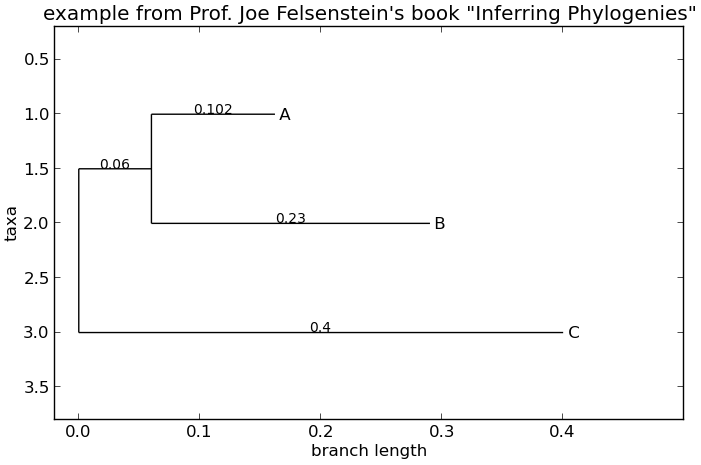
\includegraphics{phylo-draw-example.png}

\code{draw\_graphviz} 则画出一个无根的进化分枝图(cladogram),但是它要求你安装有Graphviz、
PyDot或PyGraphviz、Network和matplotlib(或pylab)。使用上面相同的例子,和Graphviz中的
\code{dot} 程序,让我们来画一个有根树(见图. {\hyperref[chr13:fig-phylo-dot]{\emph{13.3}}} ):
\DUspan{operator}{}\DUspan{name}{}\DUspan{operator}{}\DUspan{name}{}\DUspan{operator}{}\DUspan{name}{}\DUspan{punctuation}{}\DUspan{literal,string}{}\DUspan{punctuation}{}\DUspan{literal,string}{}\DUspan{punctuation}{}\DUspan{operator}{}\DUspan{name}{}\DUspan{operator}{}\DUspan{name}{}\DUspan{punctuation}{}\DUspan{name}{}\DUspan{punctuation}{}\DUspan{name}{}\DUspan{operator}{}\DUspan{literal,string}{}\DUspan{punctuation}{}\DUspan{operator}{}\DUspan{keyword,namespace}{}\DUspan{name,namespace}{}\DUspan{operator}{}\DUspan{name}{}\DUspan{operator}{}\DUspan{name}{}\DUspan{punctuation}{}\DUspan{comment}{}\DUspan{operator}{}\DUspan{name}{}\DUspan{operator}{}\DUspan{name}{}\DUspan{punctuation}{}\DUspan{literal,string}{}\DUspan{punctuation}{}\DUspan{comment}{}
\begin{Verbatim}[commandchars=\\\{\}]
\PYG{g+gp}{\PYGZgt{}\PYGZgt{}\PYGZgt{} }\PYG{n}{tree} \PYG{o}{=} \PYG{n}{Phylo}\PYG{o}{.}\PYG{n}{read}\PYG{p}{(}\PYG{l+s}{\PYGZdq{}}\PYG{l+s}{example.xml}\PYG{l+s}{\PYGZdq{}}\PYG{p}{,} \PYG{l+s}{\PYGZdq{}}\PYG{l+s}{phyloxml}\PYG{l+s}{\PYGZdq{}}\PYG{p}{)}
\PYG{g+gp}{\PYGZgt{}\PYGZgt{}\PYGZgt{} }\PYG{n}{Phylo}\PYG{o}{.}\PYG{n}{draw\PYGZus{}graphviz}\PYG{p}{(}\PYG{n}{tree}\PYG{p}{,} \PYG{n}{prog}\PYG{o}{=}\PYG{l+s}{\PYGZsq{}}\PYG{l+s}{dot}\PYG{l+s}{\PYGZsq{}}\PYG{p}{)}
\PYG{g+gp}{\PYGZgt{}\PYGZgt{}\PYGZgt{} }\PYG{k+kn}{import} \PYG{n+nn}{pylab}
\PYG{g+gp}{\PYGZgt{}\PYGZgt{}\PYGZgt{} }\PYG{n}{pylab}\PYG{o}{.}\PYG{n}{show}\PYG{p}{(}\PYG{p}{)}                    \PYG{c}{\PYGZsh{} Displays the tree in an interactive viewer}
\PYG{g+gp}{\PYGZgt{}\PYGZgt{}\PYGZgt{} }\PYG{n}{pylab}\PYG{o}{.}\PYG{n}{savefig}\PYG{p}{(}\PYG{l+s}{\PYGZsq{}}\PYG{l+s}{phylo\PYGZhy{}dot.png}\PYG{l+s}{\PYGZsq{}}\PYG{p}{)}  \PYG{c}{\PYGZsh{} Creates a PNG file of the same graphic}
\end{Verbatim}
\phantomsection\label{chr13:fig-phylo-rooted}
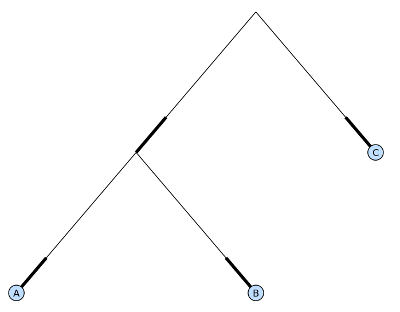
\includegraphics{phylo-dot.png}

(提示:如果你使用 \code{-pylab} 选项执行IPython,调用 \code{draw\_graphviz} 将导致matplotlib
查看器自动运行,而不需要手动的调用 \code{show()} 方法。)

这将输出树对象到一个NetworkX图中,使用Graphviz来布局节点的位置,并使用matplotlib来显示
它。这里有几个关键词参数来修改结果图像,包括大多数被NetworkX函数 \code{networkx.draw} 和
\code{networkx.draw\_graphviz} 所接受的参数。

最终的显示也受所提供的树对象的 \code{rooted} 属性的影响。有根树在每个分支(branch)上显示
一个“head”来表明它的方向(见图. {\hyperref[chr13:fig-phylo-rooted]{\emph{13.3}}} ):
\DUspan{operator}{}\DUspan{name}{}\DUspan{operator}{}\DUspan{name}{}\DUspan{operator}{}\DUspan{name}{}\DUspan{punctuation}{}\DUspan{literal,string}{}\DUspan{punctuation}{}\DUspan{literal,string}{}\DUspan{punctuation}{}\DUspan{operator}{}\DUspan{name}{}\DUspan{operator}{}\DUspan{name}{}\DUspan{operator}{}\DUspan{name,builtin,pseudo}{}\DUspan{operator}{}\DUspan{name}{}\DUspan{operator}{}\DUspan{name}{}\DUspan{punctuation}{}\DUspan{name}{}\DUspan{punctuation}{}
\begin{Verbatim}[commandchars=\\\{\}]
\PYG{g+gp}{\PYGZgt{}\PYGZgt{}\PYGZgt{} }\PYG{n}{tree} \PYG{o}{=} \PYG{n}{Phylo}\PYG{o}{.}\PYG{n}{read}\PYG{p}{(}\PYG{l+s}{\PYGZdq{}}\PYG{l+s}{simple.dnd}\PYG{l+s}{\PYGZdq{}}\PYG{p}{,} \PYG{l+s}{\PYGZdq{}}\PYG{l+s}{newick}\PYG{l+s}{\PYGZdq{}}\PYG{p}{)}
\PYG{g+gp}{\PYGZgt{}\PYGZgt{}\PYGZgt{} }\PYG{n}{tree}\PYG{o}{.}\PYG{n}{rooted} \PYG{o}{=} \PYG{n+nb+bp}{True}
\PYG{g+gp}{\PYGZgt{}\PYGZgt{}\PYGZgt{} }\PYG{n}{Phylo}\PYG{o}{.}\PYG{n}{draw\PYGZus{}graphiz}\PYG{p}{(}\PYG{n}{tree}\PYG{p}{)}
\end{Verbatim}
\phantomsection\label{chr13:fig-phylo-color}
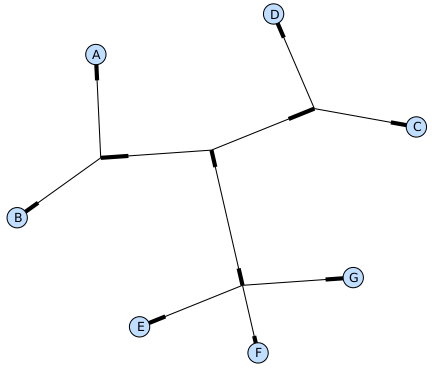
\includegraphics{phylo-rooted.png}

“prog”参数指定Graphviz的用来布局的引擎。默认的引擎 \code{twopi} 对任何大小的树都表现很好,
很可靠的避免交叉的分支出现。\code{neato} 程序可能画出更加好看的中等大小的树,但是有时候会
有交叉分支出现(见图. {\hyperref[chr13:fig-phylo-color]{\emph{13.3}}} )。 \code{dot} 程序或许对小型的树有用,
但是对于大一点的树的布局易产生奇怪的事情。
\DUspan{operator}{}\DUspan{name}{}\DUspan{operator}{}\DUspan{name}{}\DUspan{punctuation}{}\DUspan{name}{}\DUspan{punctuation}{}\DUspan{name}{}\DUspan{operator}{}\DUspan{literal,string}{}\DUspan{punctuation}{}
\begin{Verbatim}[commandchars=\\\{\}]
\PYG{g+gp}{\PYGZgt{}\PYGZgt{}\PYGZgt{} }\PYG{n}{Phylo}\PYG{o}{.}\PYG{n}{draw\PYGZus{}graphviz}\PYG{p}{(}\PYG{n}{tree}\PYG{p}{,} \PYG{n}{prog}\PYG{o}{=}\PYG{l+s}{\PYGZdq{}}\PYG{l+s}{neato}\PYG{l+s}{\PYGZdq{}}\PYG{p}{)}
\end{Verbatim}

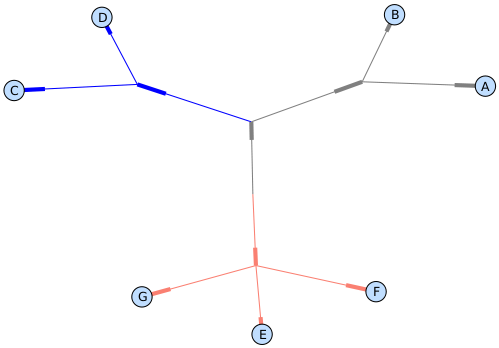
\includegraphics{phylo-color.png}

这个查看方式非常方便研究大型的树,因为matplotlib查看器可以放大选择的区域,使得杂乱的图像
变得稀疏。
\DUspan{operator}{}\DUspan{name}{}\DUspan{operator}{}\DUspan{name}{}\DUspan{operator}{}\DUspan{name}{}\DUspan{punctuation}{}\DUspan{literal,string}{}\DUspan{punctuation}{}\DUspan{literal,string}{}\DUspan{punctuation}{}\DUspan{operator}{}\DUspan{name}{}\DUspan{operator}{}\DUspan{name}{}\DUspan{punctuation}{}\DUspan{name}{}\DUspan{punctuation}{}\DUspan{name}{}\DUspan{operator}{}\DUspan{literal,string}{}\DUspan{punctuation}{}\DUspan{name}{}\DUspan{operator}{}\DUspan{literal,number,integer}{}\DUspan{punctuation}{}
\begin{Verbatim}[commandchars=\\\{\}]
\PYG{g+gp}{\PYGZgt{}\PYGZgt{}\PYGZgt{} }\PYG{n}{tree} \PYG{o}{=} \PYG{n}{Phylo}\PYG{o}{.}\PYG{n}{read}\PYG{p}{(}\PYG{l+s}{\PYGZdq{}}\PYG{l+s}{apaf.xml}\PYG{l+s}{\PYGZdq{}}\PYG{p}{,} \PYG{l+s}{\PYGZdq{}}\PYG{l+s}{phyloxml}\PYG{l+s}{\PYGZdq{}}\PYG{p}{)}
\PYG{g+gp}{\PYGZgt{}\PYGZgt{}\PYGZgt{} }\PYG{n}{Phylo}\PYG{o}{.}\PYG{n}{draw\PYGZus{}graphviz}\PYG{p}{(}\PYG{n}{tree}\PYG{p}{,} \PYG{n}{prog}\PYG{o}{=}\PYG{l+s}{\PYGZdq{}}\PYG{l+s}{neato}\PYG{l+s}{\PYGZdq{}}\PYG{p}{,} \PYG{n}{node\PYGZus{}size}\PYG{o}{=}\PYG{l+m+mi}{0}\PYG{p}{)}
\end{Verbatim}

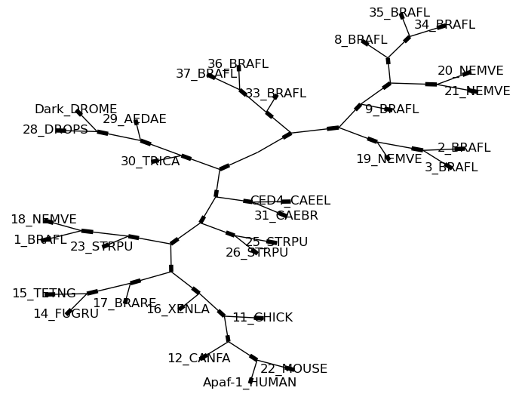
\includegraphics{phylo-apaf.png} 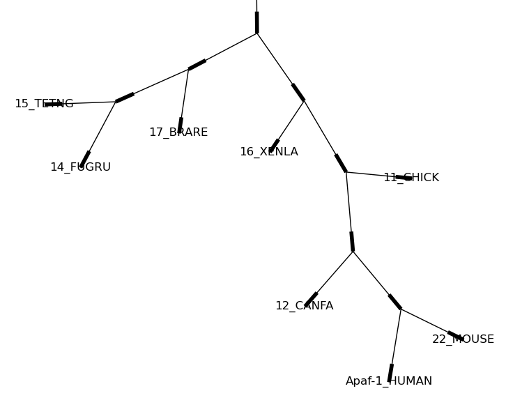
\includegraphics{phylo-apaf-zoom.png}

注意,分支长度并没有被正确地显示,因为Graphviz在布局时忽略了他们。然而,分支长度可以在输出
树为NetworkX图对象( \code{to\_networkx} )时重新获得。

查看Biopython维基的Phylo页面
(\href{http://biopython.org/wiki/Phylo}{http://biopython.org/wiki/Phylo})
以获得关于 \code{draw\_ascii} 、 \code{draw\_graphviz} 和 \code{to\_networkx} 的更加高级的功能的描述
和例子。


\section{13.4  使用Tree和Clade对象}
\label{chr13:treeclade}
\code{parse} 和 \code{read} 方法产生的 \code{Tree} 对象是一些包含递归的子树的容器,连接到 \code{Tree}
对象的 \code{root} 属性(不管进化树实际上被认为是否有根)。一个 \code{Tree} 包含进化树的全局信息,
如有根性(rootedness)和指向一个单独的 \code{Clade} 的引用; 一个 \code{Clade} 包含节点和进化枝
特异性信息,如分支长度(branch length)和一个它自身后代 \code{Clade} 实例的列表,附着在 \code{clades}
属性上。

所以,这里 \code{tree} 和 \code{tree.root} 间是有区别的. 然而,实际操作中,你几乎不需要担心它。为了
缓和这个不同,\code{Tree} 和 \code{Clade} 两者都继承自 \code{TreeMixin},它包含常用的用来查找、审视和
修改树和任何它的进化枝的方法的实现。这意味着,所有 \code{tree} 所支持的方法在 \code{tree.root} 和
任何它下面的clade中都能用。( \code{Clade} 也有一个 \code{root} 属性,它返回clade对象本身。)


\subsection{13.4.1  查找和遍历类方法}
\label{chr13:id4}
为了方便起见,我们提供了两个简化的方法来直接返回所有的外部或内部节点为列表:
\begin{description}
\item[{\textbf{{}`{}`get\_terminals{}`{}`}}] \leavevmode
创建一个包含树的所有末端(叶子)节点的列表。

\item[{\textbf{{}`{}`get\_nonterminals{}`{}`}}] \leavevmode
创建一个包含树的所有非末端(内部)节点的列表。

\end{description}

这两个都包装了一个能完全控制树的遍历的方法 \code{find\_clades}。另外两个遍历方法 \code{find\_elements}
和 \code{find\_any} 依赖于同样的核心功能,也接受同样的参数,没有更好的描述我们就把这个参数叫做
“目标说明”(target specification)吧。它们指定哪些树中的对象将被匹配并在迭代过程中返回。
第一个参数可以是下面的任何类型:
\begin{itemize}
\item {} 
一个 \textbf{TreeElement 实例} ,那个树的元素将根据一致性被匹配——这样,使用Clade实例作为目标将找到
树中的这个Clade;

\item {} 
一个 \textbf{string} ,匹配树元素的字符串表示——特别地,Clade的 \code{name} \emph{(在Biopython 1.56中引入)};

\item {} 
一个 \textbf{class} 或 \textbf{type},这样每一个类型(或子类型)相同的树元素都被匹配;

\item {} 
一个 \textbf{dictionary} ,其中键(key)是树元素的属性名,值(value)将匹配到每个树元素相应的属性值。
它变得更加详细:
\begin{itemize}
\item {} 
如果提供的是 \code{int} 类型,它将匹配数值上相等的属性,即,1将匹配1或者1.0

\item {} 
如果提供的是boolean类型(True或者False),对应的属性值将被当做boolean求值和检验

\item {} 
\code{None} 匹配 \code{None}

\item {} 
如果提供的是字符串,将被当做正则表达式对待(必须匹配对应元素属性的全部,不能只是前面的部分)。
提供没有特殊正则表达式字符的字符串将精准的匹配字符串属性,所以如果你不适用正则表达式,不用
担心它。例如,包含进化枝名称Foo1、Foo2和Foo3的一个树,
\code{tree.find\_clades(\{"name": "Foo1"\})} 将匹配 Foo1,
\code{\{"name": "Foo.*"\}} 匹配所有的三个进化枝,而
\code{\{"name": "Foo"\}} 并不匹配任何进化枝。

\end{itemize}

由于浮点数值可能产生奇怪的行为,我们不支持直接匹配 \code{float}s 类型。作为替代,使用boolean值
\code{True} 来匹配每个元素中指定属性的非零值,然后再对这个属性用不等式(或精确地数值,如果你喜欢
危险地活着)进行手动过滤。

如果该字典包含多个条目,匹配的元素必须匹配所有给定的属性值——以“and”方式思考,而不是“or”。

\item {} 
一个接受一个参数(它将应用于树中的每一个元素),返回True或False的函数 \textbf{function} 。为方便起见,
LookupError、AttributeError和ValueError被沉默,这样就提供了另外一个在树中查找浮点值的安全方式,
或者一些更加复杂的特性。

\end{itemize}

在目标参数后面,有两个可选的关键词参数:
\begin{description}
\item[{\textbf{terminal}}] \leavevmode
— 用来选择或排除末端进化枝(或者叫叶子节点)的一个boolean值:True仅搜索末端进化枝,False则搜索
非末端(内部)进化枝,而默认为None,同时搜索末端和非末端进化枝,包括没有 \code{is\_terminal} 方法的
任何树元素。

\item[{\textbf{order}}] \leavevmode
— 树遍历的顺序:\code{"preorder"} (默认值)是深度优先搜索(depth-first search,DFS), \code{"postorder"}
是子节点先于父节点的DFS搜索, \code{"level"} 是宽度优先搜索(breadth-first search,BFS)。

\end{description}

最后,这些方法接受任意的关键词参数,这些参数将被以和词典“目标说明”相同的方式对待:键表示要搜索的元素
属性的名称,参数值(string、integer、None或者boolean)将和找到的每个属性的值进行比较。如果没有提供
关键词参数,则任何TreeElement类型将被匹配。这个的代码普遍比传入一个词典作为“目标说明”要短:
\code{tree.find\_clades(\{"name": "Foo1"\})} 可以简化为 \code{tree.find\_clades(name="Foo1")}。

(在Biopython 1.56和以后的版本中,这可以更短:\code{tree.find\_clades("Foo1")} )

现在我们已经掌握了“目标说明”,这里有一些遍历树的方法:
\begin{description}
\item[{\textbf{{}`{}`find\_clades{}`{}`}}] \leavevmode
查找每个包含匹配元素的进化枝。就是说,用 \code{find\_elements} 查找每个元素,然而返回对应的clade对象。
(这通常是你想要的。)

最终的结果是一个包含所有匹配对象的迭代器,默认为深度优先搜索。这不一定是和Newick、Nexus或XML原文件
中显示的相同的顺序。

\item[{\textbf{{}`{}`find\_elements{}`{}`}}] \leavevmode\begin{description}
\item[{查找和给定属性匹配的所有树元素,返回匹配的元素本身。简单的Newick树没有复杂的子元素,所以它将和}] \leavevmode
\code{find\_clades} 的行为一致。PhyloXML树通常在clade上附加有复杂的对象,所以这个方法对提取这些信息
非常有用。

\end{description}

\item[{\textbf{{}`{}`find\_any{}`{}`}}] \leavevmode
返回 \code{find\_elements()} 所找到的第一个元素,或者None。这对于检测树中是否存在匹配的元素也非常有用,
可以在条件判断语句中使用。

\end{description}

另外两个用于帮助在树的节点间导航的方法:
\begin{description}
\item[{\textbf{{}`{}`get\_path{}`{}`}}] \leavevmode
直接列出从树的根节点(或当前进化枝)到给定的目标间的所有clade。返回包含这个路径上所有clade对象的
列表,以给定目标为结尾,但不包含根进化枝。

\item[{\textbf{{}`{}`trace{}`{}`}}] \leavevmode
列出树中两个目标间的所有clade对象,不包含起始和结尾。

\end{description}


\subsection{13.4.2  信息类方法}
\label{chr13:id5}
这些方法提供关于整个树(或任何进化枝)的信息。
\begin{description}
\item[{\textbf{{}`{}`common\_ancestor{}`{}`}}] \leavevmode
查找所提供的所有目标的最近共同祖先(the most recent common ancestor)
(这将是一个Clade对象)。如果没有提供任何目标,将返回当前Clade(调用该
方法的那个)的根;如果提供一个目标,将返回目标本身。然而,如果有任何提供
的目标无法在当前tree(或clade)中找到,将引起一个异常。

\item[{\textbf{{}`{}`count\_terminals{}`{}`}}] \leavevmode
计算树中末端(叶子)节点的个数。

\item[{\textbf{{}`{}`depths{}`{}`}}] \leavevmode
创建一个树中进化枝到其深度的映射。结果是一个字典,其中键是树中所有的Clade
实例,值是从根到每个clade(包含末端)的距离。默认距离是到这个clade的分支
长度累加,然而使用 \code{unit\_branch\_lengths=True} 选项,将只计算分支的个数
(其在树中的级数)。

\item[{\textbf{{}`{}`distance{}`{}`}}] \leavevmode
计算两个目标间的分支长度总和。如果只指定一个目标,另一个则为该树的根。

\item[{\textbf{{}`{}`total\_branch\_length{}`{}`}}] \leavevmode
计算这个树中的分支长度总和。这在系统发生学中通常就称为树的长度“length”,
但是我们使用更加明确的名称,以避免和Python的术语混淆。

\end{description}

余下的方法是boolean检测方法:
\begin{description}
\item[{\textbf{{}`{}`is\_bifurcating{}`{}`}}] \leavevmode
如果树是严格的二叉树;即,所有的节点有2个或者0个子代(对应的,内部或外部)。
根节点可能有三个后代,然而仍然被认为是二叉树的一部分。

\item[{\textbf{{}`{}`is\_monophyletic{}`{}`}}] \leavevmode
检验给定的所有目标是否组成一个完成的子进化枝——即,存在一个进化枝满足:它的
末端节点和给定的目标是相同的集合。目标需要时树中的末端节点。为方便起见,若
给定目标是一个单系(monophyletic),这个方法将返回它们的共同祖先(MCRA)(
而不是 \code{True} ),否则将返回 \code{False} 。

\item[{\textbf{{}`{}`is\_parent\_of{}`{}`}}] \leavevmode
若目标是这个树的后代(descendant)则为True——不必为直接后代。检验一个进化枝的
直接后代,只需要用简单的列表成员检测方法: \code{if subclade in clade: ...}

\item[{\textbf{{}`{}`is\_preterminal{}`{}`}}] \leavevmode
若所有的直接后代都为末端则为True;否则任何一个直接后代不为末端则为False。

\end{description}


\subsection{13.4.3  修改类方法}
\label{chr13:id6}
这些方法都在原地对树进行修改,所以如果你想保持原来的树不变,你首先要使用Python的
\code{copy} 模块对树进行完整的拷贝:
\DUspan{name}{}\DUspan{operator}{}\DUspan{name}{}\DUspan{operator}{}\DUspan{name}{}\DUspan{punctuation}{}\DUspan{literal,string}{}\DUspan{punctuation}{}\DUspan{literal,string}{}\DUspan{punctuation}{}\DUspan{keyword,namespace}{}\DUspan{name,namespace}{}\DUspan{name}{}\DUspan{operator}{}\DUspan{name}{}\DUspan{operator}{}\DUspan{name}{}\DUspan{punctuation}{}\DUspan{name}{}\DUspan{punctuation}{}
\begin{Verbatim}[commandchars=\\\{\}]
\PYG{n}{tree} \PYG{o}{=} \PYG{n}{Phylo}\PYG{o}{.}\PYG{n}{read}\PYG{p}{(}\PYG{l+s}{\PYGZsq{}}\PYG{l+s}{example.xml}\PYG{l+s}{\PYGZsq{}}\PYG{p}{,} \PYG{l+s}{\PYGZsq{}}\PYG{l+s}{phyloxml}\PYG{l+s}{\PYGZsq{}}\PYG{p}{)}
\PYG{k+kn}{import} \PYG{n+nn}{copy}
\PYG{n}{newtree} \PYG{o}{=} \PYG{n}{copy}\PYG{o}{.}\PYG{n}{deepcopy}\PYG{p}{(}\PYG{n}{tree}\PYG{p}{)}
\end{Verbatim}
\begin{description}
\item[{\textbf{{}`{}`collapse{}`{}`}}] \leavevmode
从树中删除目标,重新连接它的子代(children)到它的父亲节点(parent)。

\item[{\textbf{{}`{}`collapse\_all{}`{}`}}] \leavevmode
删除这个树的所有后代(descendants),只保留末端节点(terminals)。
分支长度被保留,即到每个末端节点的距离保持不变。如指定一个目标(见上),
只坍塌(collapses)和指定匹配的内部节点。

\item[{\textbf{{}`{}`ladderize{}`{}`}}] \leavevmode
根据末端节点的个数,在原地对进化枝(clades)进行排序。越深的进化枝默认被放到最后,
使用 \code{reverse=True} 将其放到最前。

\item[{\textbf{{}`{}`prune{}`{}`}}] \leavevmode
从树中修剪末端进化枝(terminal clade)。如果分类名(taxon)来自一个二叉枝(bifurcation),
连接的节点将被坍塌,它的分支长度将被加到剩下的末端节点上。这可能不再是一个有意义的值。

\item[{\textbf{{}`{}`root\_with\_outgroup{}`{}`}}] \leavevmode
使用包含给定目标的外群进化枝(outgroup clade)重新确定树的根节点,即外群的共同祖先。该方法
只在Tree对象中能用,不能用于Clade对象。

如果外群和self.root一致,将不发生改变。如果外群进化枝是末端(即一个末端节点被作为外群),一个
新的二叉根进化枝将被创建,且到给定外群的分支长度为0。否则,外群根部的内部节点变为整个树的一个
三叉根。如果原先的根是一个二叉,它将被从树中遗弃。

在所有的情况下,树的分支长度总和保持不变。

\item[{\textbf{{}`{}`root\_at\_midpoint{}`{}`}}] \leavevmode
重新选择树中两个最远的节点的中点作为树的根。(这实际上是使用 \code{root\_with\_outgroup} 函数。)

\item[{\textbf{{}`{}`split{}`{}`}}] \leavevmode
产生 \emph{n} (默认为2)个 新的后代。在一个物种树中,这是一个物种形成事件。新的进化枝拥有给定的
\code{branch\_length} 以及和这个进化枝的根相同的名字,名字后面包含一个整数后缀(从0开始计数)——
例如,分割名为“A”的进化枝将生成子进化枝“A0”和“A1”。

\end{description}

查看Biopython维基的Phylo页面
(\href{http://biopython.org/wiki/Phylo}{http://biopython.org/wiki/Phylo})
以获得更多已有方法的使用示例。


\subsection{13.4.4  PhyloXML树的特性}
\label{chr13:phyloxml}\label{chr13:sec-phyloxml}
phyloXML文件格式包含用来注释树的,采用额外数据格式和图像提示的字段。

参加Biopython维基上的PhyloXML页面
(\href{http://biopython.org/wiki/PhyloXML}{http://biopython.org/wiki/PhyloXML})
以查看关于使用PhyloXML提供的额外注释特性的描述和例子。


\section{13.5  运行外部程序}
\label{chr13:id7}
尽管Bio.Phylo本身不从序列比对推断进化树,但这里有一些第三方的程序可以使用。
他们通过 \code{Bio.Phylo.Applications} 模块获得支持,使用和 \code{Bio.Emboss.Applications} 、
\code{Bio.Align.Applications} 以及其他模块相同的通用框架。

Biopython 1.58引入了一个PhyML的打包程序(wrapper)
(\href{http://www.atgc-montpellier.fr/phyml/}{http://www.atgc-montpellier.fr/phyml/})。
该程序接受一个 \code{phylip-relaxed} 格式(它是Phylip格式,然而没有对分类名称的10个字符的限制)
的比对输入和多种参数。一个快速的例子是:
\DUspan{operator}{}\DUspan{keyword,namespace}{}\DUspan{name,namespace}{}\DUspan{keyword,namespace}{}\DUspan{name}{}\DUspan{operator}{}\DUspan{keyword,namespace}{}\DUspan{name,namespace}{}\DUspan{keyword,namespace}{}\DUspan{name}{}\DUspan{operator}{}\DUspan{name}{}\DUspan{operator}{}\DUspan{name}{}\DUspan{punctuation}{}\DUspan{name,builtin}{}\DUspan{operator}{}\DUspan{literal,string}{}\DUspan{punctuation}{}\DUspan{operator}{}\DUspan{name}{}\DUspan{punctuation}{}\DUspan{name}{}\DUspan{operator}{}\DUspan{name}{}\DUspan{punctuation}{}
\begin{Verbatim}[commandchars=\\\{\}]
\PYG{g+gp}{\PYGZgt{}\PYGZgt{}\PYGZgt{} }\PYG{k+kn}{from} \PYG{n+nn}{Bio} \PYG{k+kn}{import} \PYG{n}{Phylo}
\PYG{g+gp}{\PYGZgt{}\PYGZgt{}\PYGZgt{} }\PYG{k+kn}{from} \PYG{n+nn}{Bio.Phylo.Applications} \PYG{k+kn}{import} \PYG{n}{PhymlCommandline}
\PYG{g+gp}{\PYGZgt{}\PYGZgt{}\PYGZgt{} }\PYG{n}{cmd} \PYG{o}{=} \PYG{n}{PhymlCommandline}\PYG{p}{(}\PYG{n+nb}{input}\PYG{o}{=}\PYG{l+s}{\PYGZsq{}}\PYG{l+s}{Tests/Phylip/random.phy}\PYG{l+s}{\PYGZsq{}}\PYG{p}{)}
\PYG{g+gp}{\PYGZgt{}\PYGZgt{}\PYGZgt{} }\PYG{n}{out\PYGZus{}log}\PYG{p}{,} \PYG{n}{err\PYGZus{}log} \PYG{o}{=} \PYG{n}{cmd}\PYG{p}{(}\PYG{p}{)}
\end{Verbatim}

这生成一个树文件盒一个统计文件,名称为:
{[}\emph{input filename}{]}\code{\_phyml\_tree.txt} 和
{[}\emph{input filename}{]}\code{\_phyml\_stats.txt}. 树文件的格式是Newick格式:
\DUspan{operator}{}\DUspan{name}{}\DUspan{operator}{}\DUspan{name}{}\DUspan{operator}{}\DUspan{name}{}\DUspan{punctuation}{}\DUspan{literal,string}{}\DUspan{punctuation}{}\DUspan{literal,string}{}\DUspan{punctuation}{}\DUspan{operator}{}\DUspan{name}{}\DUspan{operator}{}\DUspan{name}{}\DUspan{punctuation}{}\DUspan{name}{}\DUspan{punctuation}{}
\begin{Verbatim}[commandchars=\\\{\}]
\PYG{g+gp}{\PYGZgt{}\PYGZgt{}\PYGZgt{} }\PYG{n}{tree} \PYG{o}{=} \PYG{n}{Phylo}\PYG{o}{.}\PYG{n}{read}\PYG{p}{(}\PYG{l+s}{\PYGZsq{}}\PYG{l+s}{Tests/Phylip/random.phy\PYGZus{}phyml\PYGZus{}tree.txt}\PYG{l+s}{\PYGZsq{}}\PYG{p}{,} \PYG{l+s}{\PYGZsq{}}\PYG{l+s}{newick}\PYG{l+s}{\PYGZsq{}}\PYG{p}{)}
\PYG{g+gp}{\PYGZgt{}\PYGZgt{}\PYGZgt{} }\PYG{n}{Phylo}\PYG{o}{.}\PYG{n}{draw\PYGZus{}ascii}\PYG{p}{(}\PYG{n}{tree}\PYG{p}{)}
\end{Verbatim}

一个类似的RAxML打包程序
(\href{http://sco.h-its.org/exelixis/software.html}{http://sco.h-its.org/exelixis/software.html})
也已经被添加到Biopython 1.60中。

注意,如果你系统中已经安装了EMBOSS的Phylip扩展,一些常用的Phylip程序,包括 \code{dnaml} 和 \code{protml}
已经通过 \code{Bio.Emboss.Applications} 中的EMBOSS打包程序被支持。参见章节 {\hyperref[chr06:sec-alignment-tools]{\emph{6.4}}}
以查看使用这些程序的例子和提示。


\section{13.6  PAML整合}
\label{chr13:paml}
Biopython 1.58引入了对PAML的支持
(\href{http://abacus.gene.ucl.ac.uk/software/paml.html}{http://abacus.gene.ucl.ac.uk/software/paml.html}),
它是一个采用最大似然法(maximum likelihood)进行系统进化分析的程序包。目前,对程序codeml、baseml和yn00的支持
已经实现。由于PAML使用控制文件而不是命令行参数来控制运行时选项,这个打包程序(wrapper)的使用格式和Biopython
的其他应用打包程序有些差异。

一个典型的流程是:初始化一个PAML对象,指定一个比对文件,一个树文件,一个输出文件和工作路径。下一步,运行时
选项通过 \code{set\_options()} 方法或者读入一个已有的控制文件来设定。最后,程序通过 \code{run()} 方法来运行,输出文件
将自动被解析到一个结果目录。

下面是一个codeml典型用法的例子:
\DUspan{operator}{}\DUspan{keyword,namespace}{}\DUspan{name,namespace}{}\DUspan{keyword,namespace}{}\DUspan{name}{}\DUspan{operator}{}\DUspan{name}{}\DUspan{operator}{}\DUspan{name}{}\DUspan{operator}{}\DUspan{name}{}\DUspan{punctuation}{}\DUspan{operator}{}\DUspan{name}{}\DUspan{operator}{}\DUspan{name}{}\DUspan{operator}{}\DUspan{literal,string}{}\DUspan{operator}{}\DUspan{name}{}\DUspan{operator}{}\DUspan{name}{}\DUspan{operator}{}\DUspan{literal,string}{}\DUspan{operator}{}\DUspan{name}{}\DUspan{operator}{}\DUspan{name}{}\DUspan{operator}{}\DUspan{literal,string}{}\DUspan{operator}{}\DUspan{name}{}\DUspan{operator}{}\DUspan{name}{}\DUspan{operator}{}\DUspan{literal,string}{}\DUspan{operator}{}\DUspan{name}{}\DUspan{operator}{}\DUspan{name}{}\DUspan{punctuation}{}\DUspan{name}{}\DUspan{operator}{}\DUspan{literal,number,integer}{}\DUspan{punctuation}{}\DUspan{operator}{}\DUspan{name}{}\DUspan{operator}{}\DUspan{literal,number,integer}{}\DUspan{punctuation}{}\DUspan{operator}{}\DUspan{name}{}\DUspan{operator}{}\DUspan{literal,number,integer}{}\DUspan{punctuation}{}\DUspan{operator}{}\DUspan{name}{}\DUspan{operator}{}\DUspan{literal,number,integer}{}\DUspan{punctuation}{}\DUspan{operator}{}\DUspan{name}{}\DUspan{operator}{}\DUspan{literal,number,integer}{}\DUspan{punctuation}{}\DUspan{operator}{}\DUspan{name}{}\DUspan{operator}{}\DUspan{punctuation}{}\DUspan{literal,number,integer}{}\DUspan{punctuation}{}\DUspan{literal,number,integer}{}\DUspan{punctuation}{}\DUspan{literal,number,integer}{}\DUspan{punctuation}{}\DUspan{operator}{}\DUspan{name}{}\DUspan{operator}{}\DUspan{literal,number,integer}{}\DUspan{punctuation}{}\DUspan{operator}{}\DUspan{name}{}\DUspan{operator}{}\DUspan{literal,number,integer}{}\DUspan{punctuation}{}\DUspan{operator}{}\DUspan{name}{}\DUspan{operator}{}\DUspan{literal,number,integer}{}\DUspan{punctuation}{}\DUspan{operator}{}\DUspan{name}{}\DUspan{operator}{}\DUspan{literal,number,float}{}\DUspan{punctuation}{}\DUspan{operator}{}\DUspan{name}{}\DUspan{operator}{}\DUspan{name}{}\DUspan{operator}{}\DUspan{name}{}\DUspan{punctuation}{}\DUspan{operator}{}\DUspan{name}{}\DUspan{operator}{}\DUspan{name}{}\DUspan{operator}{}\DUspan{name}{}\DUspan{punctuation}{}\DUspan{literal,string}{}\DUspan{punctuation}{}\DUspan{operator}{}\DUspan{name}{}\DUspan{operator}{}\DUspan{name}{}\DUspan{operator}{}\DUspan{name}{}\DUspan{punctuation}{}\DUspan{literal,number,integer}{}\DUspan{punctuation}{}\DUspan{operator}{}\DUspan{name}{}\DUspan{operator}{}\DUspan{name}{}\DUspan{operator}{}\DUspan{name}{}\DUspan{punctuation}{}\DUspan{literal,string}{}\DUspan{punctuation}{}\DUspan{operator}{}\DUspan{keyword}{}\DUspan{name}{}\DUspan{operator}{}\DUspan{name}{}\DUspan{punctuation}{}\DUspan{literal,string}{}\DUspan{punctuation}{}
\begin{Verbatim}[commandchars=\\\{\}]
\PYG{g+gp}{\PYGZgt{}\PYGZgt{}\PYGZgt{} }\PYG{k+kn}{from} \PYG{n+nn}{Bio.Phylo.PAML} \PYG{k+kn}{import} \PYG{n}{codeml}
\PYG{g+gp}{\PYGZgt{}\PYGZgt{}\PYGZgt{} }\PYG{n}{cml} \PYG{o}{=} \PYG{n}{codeml}\PYG{o}{.}\PYG{n}{Codeml}\PYG{p}{(}\PYG{p}{)}
\PYG{g+gp}{\PYGZgt{}\PYGZgt{}\PYGZgt{} }\PYG{n}{cml}\PYG{o}{.}\PYG{n}{alignment} \PYG{o}{=} \PYG{l+s}{\PYGZdq{}}\PYG{l+s}{Tests/PAML/alignment.phylip}\PYG{l+s}{\PYGZdq{}}
\PYG{g+gp}{\PYGZgt{}\PYGZgt{}\PYGZgt{} }\PYG{n}{cml}\PYG{o}{.}\PYG{n}{tree} \PYG{o}{=} \PYG{l+s}{\PYGZdq{}}\PYG{l+s}{Tests/PAML/species.tree}\PYG{l+s}{\PYGZdq{}}
\PYG{g+gp}{\PYGZgt{}\PYGZgt{}\PYGZgt{} }\PYG{n}{cml}\PYG{o}{.}\PYG{n}{out\PYGZus{}file} \PYG{o}{=} \PYG{l+s}{\PYGZdq{}}\PYG{l+s}{results.out}\PYG{l+s}{\PYGZdq{}}
\PYG{g+gp}{\PYGZgt{}\PYGZgt{}\PYGZgt{} }\PYG{n}{cml}\PYG{o}{.}\PYG{n}{working\PYGZus{}dir} \PYG{o}{=} \PYG{l+s}{\PYGZdq{}}\PYG{l+s}{./scratch}\PYG{l+s}{\PYGZdq{}}
\PYG{g+gp}{\PYGZgt{}\PYGZgt{}\PYGZgt{} }\PYG{n}{cml}\PYG{o}{.}\PYG{n}{set\PYGZus{}options}\PYG{p}{(}\PYG{n}{seqtype}\PYG{o}{=}\PYG{l+m+mi}{1}\PYG{p}{,}
\PYG{g+gp}{... }        \PYG{n}{verbose}\PYG{o}{=}\PYG{l+m+mi}{0}\PYG{p}{,}
\PYG{g+gp}{... }        \PYG{n}{noisy}\PYG{o}{=}\PYG{l+m+mi}{0}\PYG{p}{,}
\PYG{g+gp}{... }        \PYG{n}{RateAncestor}\PYG{o}{=}\PYG{l+m+mi}{0}\PYG{p}{,}
\PYG{g+gp}{... }        \PYG{n}{model}\PYG{o}{=}\PYG{l+m+mi}{0}\PYG{p}{,}
\PYG{g+gp}{... }        \PYG{n}{NSsites}\PYG{o}{=}\PYG{p}{[}\PYG{l+m+mi}{0}\PYG{p}{,} \PYG{l+m+mi}{1}\PYG{p}{,} \PYG{l+m+mi}{2}\PYG{p}{]}\PYG{p}{,}
\PYG{g+gp}{... }        \PYG{n}{CodonFreq}\PYG{o}{=}\PYG{l+m+mi}{2}\PYG{p}{,}
\PYG{g+gp}{... }        \PYG{n}{cleandata}\PYG{o}{=}\PYG{l+m+mi}{1}\PYG{p}{,}
\PYG{g+gp}{... }        \PYG{n}{fix\PYGZus{}alpha}\PYG{o}{=}\PYG{l+m+mi}{1}\PYG{p}{,}
\PYG{g+gp}{... }        \PYG{n}{kappa}\PYG{o}{=}\PYG{l+m+mf}{4.54006}\PYG{p}{)}
\PYG{g+gp}{\PYGZgt{}\PYGZgt{}\PYGZgt{} }\PYG{n}{results} \PYG{o}{=} \PYG{n}{cml}\PYG{o}{.}\PYG{n}{run}\PYG{p}{(}\PYG{p}{)}
\PYG{g+gp}{\PYGZgt{}\PYGZgt{}\PYGZgt{} }\PYG{n}{ns\PYGZus{}sites} \PYG{o}{=} \PYG{n}{results}\PYG{o}{.}\PYG{n}{get}\PYG{p}{(}\PYG{l+s}{\PYGZdq{}}\PYG{l+s}{NSsites}\PYG{l+s}{\PYGZdq{}}\PYG{p}{)}
\PYG{g+gp}{\PYGZgt{}\PYGZgt{}\PYGZgt{} }\PYG{n}{m0} \PYG{o}{=} \PYG{n}{ns\PYGZus{}sites}\PYG{o}{.}\PYG{n}{get}\PYG{p}{(}\PYG{l+m+mi}{0}\PYG{p}{)}
\PYG{g+gp}{\PYGZgt{}\PYGZgt{}\PYGZgt{} }\PYG{n}{m0\PYGZus{}params} \PYG{o}{=} \PYG{n}{m0}\PYG{o}{.}\PYG{n}{get}\PYG{p}{(}\PYG{l+s}{\PYGZdq{}}\PYG{l+s}{parameters}\PYG{l+s}{\PYGZdq{}}\PYG{p}{)}
\PYG{g+gp}{\PYGZgt{}\PYGZgt{}\PYGZgt{} }\PYG{k}{print} \PYG{n}{m0\PYGZus{}params}\PYG{o}{.}\PYG{n}{get}\PYG{p}{(}\PYG{l+s}{\PYGZdq{}}\PYG{l+s}{omega}\PYG{l+s}{\PYGZdq{}}\PYG{p}{)}
\end{Verbatim}

已有的输出文件也可以通过模块的 \code{read()} 方法来解析:
\DUspan{operator}{}\DUspan{name}{}\DUspan{operator}{}\DUspan{name}{}\DUspan{operator}{}\DUspan{name}{}\DUspan{punctuation}{}\DUspan{literal,string}{}\DUspan{punctuation}{}\DUspan{operator}{}\DUspan{keyword}{}\DUspan{name}{}\DUspan{operator}{}\DUspan{name}{}\DUspan{punctuation}{}\DUspan{literal,string}{}\DUspan{punctuation}{}
\begin{Verbatim}[commandchars=\\\{\}]
\PYG{g+gp}{\PYGZgt{}\PYGZgt{}\PYGZgt{} }\PYG{n}{results} \PYG{o}{=} \PYG{n}{codeml}\PYG{o}{.}\PYG{n}{read}\PYG{p}{(}\PYG{l+s}{\PYGZdq{}}\PYG{l+s}{Tests/PAML/Results/codeml/codeml\PYGZus{}NSsites\PYGZus{}all.out}\PYG{l+s}{\PYGZdq{}}\PYG{p}{)}
\PYG{g+gp}{\PYGZgt{}\PYGZgt{}\PYGZgt{} }\PYG{k}{print} \PYG{n}{results}\PYG{o}{.}\PYG{n}{get}\PYG{p}{(}\PYG{l+s}{\PYGZdq{}}\PYG{l+s}{lnL max}\PYG{l+s}{\PYGZdq{}}\PYG{p}{)}
\end{Verbatim}

这个新模块的详细介绍目前在Biopython维基上可以看到:
\href{http://biopython.org/wiki/PAML}{http://biopython.org/wiki/PAML}


\section{13.7  未来计划}
\label{chr13:id8}
Bio.Phylo 目前还在开发中,下面是我们可能会在将来的发布版本中添加的特性:
\begin{description}
\item[{\textbf{新方法}}] \leavevmode
通常用来操作Tree和Clade对象的有用方法会首先出现在Biopython维基上,这样常规用户
就能在我们添加到Bio.Phylo之前测试这些方法,看看它们是否有用:
\href{http://biopython.org/wiki/Phylo\_cookbook}{http://biopython.org/wiki/Phylo\_cookbook}

\item[{\textbf{Bio.Nexus port}}] \leavevmode
这个模块的大部分是在2009年NESCent主办的谷歌编程夏令营中写的,作为实现Python对phyloXML数据格式(见
{\hyperref[chr13:sec-phyloxml]{\emph{13.4.4}}} )支持的一个项目。对Newick和Nexus格式的支持,已经通过导入Bio.Nexus模块
的一部分被添加到Bio.Phylo使用的新类中。

目前,Bio.Nexus包含一些还没有导入到Bio.Phylo类中的有用的特性——特别是,计算一致树(consensus tree)。
如果你发现某些功能Bio.Phylo中没有,试试在Bio.Nexus中能不能找到。

\end{description}

我们乐意接受任何增强该模块功能和使用性的建议;如果有,只需要通过邮件列表或我们的bug数据库让我们知道。


\chapter{第14章   使用Bio.motifs进行模体序列分析}
\label{chr14::doc}\label{chr14:bio-motifs}
这章主要的介绍Biopython中的 \code{Bio.motifs} 包。这个包是为了方便那些需要进行模体序列分析的人们而特意提供的,所以我想你们在使用时肯定对模体序列分析的一些相关要点都很熟悉。假如在使用中遇到不清楚的地方,请您查阅 {\hyperref[chr14:sec-links]{\emph{14.8}}} 相关章节以获得有关的信息。

这章的大部分内容是介绍Biopython 1.61 之前版本中新加入的 \code{Bio.motifs} 包,该包替代了Biopython 1.50版本中的 \code{Bio.Motif} 包,而 \code{Bio.Motif} 包是基于较早版本的Biopython 中的两个模块 \code{Bio.AlignAce} 和 \code{Bio.MEME} 。\code{Bio.motifs} 包较好地综合了上述的几个模块的功能,做为一个统一模块工具。

说到其他库,看到这里,你或许会对 \href{http://fraenkel.mit.edu/TAMO/}{TAMO} 感兴趣,这是另一个分析模体序列的Python库。它能提供更多关于 \emph{de-novo} 模体的查找方式,不过它并没有纳入到Biopython中,而且在商业用途上还有一些限制。


\section{14.1  模体对象}
\label{chr14:id1}
由于我们感兴趣的是模体分析,所以我们需要先看看 \code{Motif} 对象。对此我们需要先导入Bio.motifs包:
\DUspan{operator}{}\DUspan{keyword,namespace}{}\DUspan{name,namespace}{}\DUspan{keyword,namespace}{}\DUspan{name}{}
\begin{Verbatim}[commandchars=\\\{\}]
\PYG{g+gp}{\PYGZgt{}\PYGZgt{}\PYGZgt{} }\PYG{k+kn}{from} \PYG{n+nn}{Bio} \PYG{k+kn}{import} \PYG{n}{motifs}
\end{Verbatim}

然后我们可以开始创建我们第一个模体对象。我们可以从模体的实例列表中创建一个 \code{Motif} 对象,也可以通过读取模体数据库中或模体查找软件产生的文件来获得一个 \code{Motif} 对象。
\DUspan{operator}{}\DUspan{keyword,namespace}{}\DUspan{name,namespace}{}\DUspan{keyword,namespace}{}\DUspan{name}{}
\begin{Verbatim}[commandchars=\\\{\}]
\PYG{g+gp}{\PYGZgt{}\PYGZgt{}\PYGZgt{} }\PYG{k+kn}{from} \PYG{n+nn}{Bio} \PYG{k+kn}{import} \PYG{n}{motifs}
\end{Verbatim}


\subsection{14.1.1  从实例中创建一个模体}
\label{chr14:id2}
假设我们有一些DNA模体的实例:
\DUspan{operator}{}\DUspan{keyword,namespace}{}\DUspan{name,namespace}{}\DUspan{keyword,namespace}{}\DUspan{name}{}\DUspan{operator}{}\DUspan{name}{}\DUspan{operator}{}\DUspan{punctuation}{}\DUspan{name}{}\DUspan{punctuation}{}\DUspan{literal,string}{}\DUspan{punctuation}{}\DUspan{operator}{}\DUspan{name}{}\DUspan{punctuation}{}\DUspan{literal,string}{}\DUspan{punctuation}{}\DUspan{operator}{}\DUspan{name}{}\DUspan{punctuation}{}\DUspan{literal,string}{}\DUspan{punctuation}{}\DUspan{operator}{}\DUspan{name}{}\DUspan{punctuation}{}\DUspan{literal,string}{}\DUspan{punctuation}{}\DUspan{operator}{}\DUspan{name}{}\DUspan{punctuation}{}\DUspan{literal,string}{}\DUspan{punctuation}{}\DUspan{operator}{}\DUspan{name}{}\DUspan{punctuation}{}\DUspan{literal,string}{}\DUspan{punctuation}{}\DUspan{operator}{}\DUspan{name}{}\DUspan{punctuation}{}\DUspan{literal,string}{}\DUspan{punctuation}{}\DUspan{operator}{}\DUspan{punctuation}{}
\begin{Verbatim}[commandchars=\\\{\}]
\PYG{g+gp}{\PYGZgt{}\PYGZgt{}\PYGZgt{} }\PYG{k+kn}{from} \PYG{n+nn}{Bio.Seq} \PYG{k+kn}{import} \PYG{n}{Seq}
\PYG{g+gp}{\PYGZgt{}\PYGZgt{}\PYGZgt{} }\PYG{n}{instances} \PYG{o}{=} \PYG{p}{[}\PYG{n}{Seq}\PYG{p}{(}\PYG{l+s}{\PYGZdq{}}\PYG{l+s}{TACAA}\PYG{l+s}{\PYGZdq{}}\PYG{p}{)}\PYG{p}{,}
\PYG{g+gp}{... }             \PYG{n}{Seq}\PYG{p}{(}\PYG{l+s}{\PYGZdq{}}\PYG{l+s}{TACGC}\PYG{l+s}{\PYGZdq{}}\PYG{p}{)}\PYG{p}{,}
\PYG{g+gp}{... }             \PYG{n}{Seq}\PYG{p}{(}\PYG{l+s}{\PYGZdq{}}\PYG{l+s}{TACAC}\PYG{l+s}{\PYGZdq{}}\PYG{p}{)}\PYG{p}{,}
\PYG{g+gp}{... }             \PYG{n}{Seq}\PYG{p}{(}\PYG{l+s}{\PYGZdq{}}\PYG{l+s}{TACCC}\PYG{l+s}{\PYGZdq{}}\PYG{p}{)}\PYG{p}{,}
\PYG{g+gp}{... }             \PYG{n}{Seq}\PYG{p}{(}\PYG{l+s}{\PYGZdq{}}\PYG{l+s}{AACCC}\PYG{l+s}{\PYGZdq{}}\PYG{p}{)}\PYG{p}{,}
\PYG{g+gp}{... }             \PYG{n}{Seq}\PYG{p}{(}\PYG{l+s}{\PYGZdq{}}\PYG{l+s}{AATGC}\PYG{l+s}{\PYGZdq{}}\PYG{p}{)}\PYG{p}{,}
\PYG{g+gp}{... }             \PYG{n}{Seq}\PYG{p}{(}\PYG{l+s}{\PYGZdq{}}\PYG{l+s}{AATGC}\PYG{l+s}{\PYGZdq{}}\PYG{p}{)}\PYG{p}{,}
\PYG{g+gp}{... }            \PYG{p}{]}
\end{Verbatim}

然后我们可以如下创建一个模体对象:
\DUspan{operator}{}\DUspan{name}{}\DUspan{operator}{}\DUspan{name}{}\DUspan{operator}{}\DUspan{name}{}\DUspan{punctuation}{}\DUspan{name}{}\DUspan{punctuation}{}
\begin{Verbatim}[commandchars=\\\{\}]
\PYG{g+gp}{\PYGZgt{}\PYGZgt{}\PYGZgt{} }\PYG{n}{m} \PYG{o}{=} \PYG{n}{motifs}\PYG{o}{.}\PYG{n}{create}\PYG{p}{(}\PYG{n}{instances}\PYG{p}{)}
\end{Verbatim}

这些实例被存储在一个名为 \code{m.instances} 的属性中,这个其实也就是一个Python的列表,只不过附加了一些功能,这些功能将在之后介绍。将这些模体对象打印出来后就可以看出这些实例是从哪构建出来的。
\DUspan{operator}{}\DUspan{keyword}{}\DUspan{name}{}\DUspan{name}{}\DUspan{name}{}\DUspan{name}{}\DUspan{name}{}\DUspan{name}{}\DUspan{name}{}\DUspan{name}{}\DUspan{operator}{}\DUspan{name}{}\DUspan{operator}{}
\begin{Verbatim}[commandchars=\\\{\}]
\PYG{g+gp}{\PYGZgt{}\PYGZgt{}\PYGZgt{} }\PYG{k}{print} \PYG{n}{m}
\PYG{g+go}{TACAA}
\PYG{g+go}{TACGC}
\PYG{g+go}{TACAC}
\PYG{g+go}{TACCC}
\PYG{g+go}{AACCC}
\PYG{g+go}{AATGC}
\PYG{g+go}{AATGC}
\end{Verbatim}

模体的长度像其他一些实例一些被定义为序列的长度:
\DUspan{operator}{}\DUspan{name,builtin}{}\DUspan{punctuation}{}\DUspan{name}{}\DUspan{punctuation}{}\DUspan{literal,number,integer}{}
\begin{Verbatim}[commandchars=\\\{\}]
\PYG{g+gp}{\PYGZgt{}\PYGZgt{}\PYGZgt{} }\PYG{n+nb}{len}\PYG{p}{(}\PYG{n}{m}\PYG{p}{)}
\PYG{g+go}{5}
\end{Verbatim}

模体对象有一个 \code{.counts} 属性,可以用来查看碱基在每个位置的数目。可以把这个统计表用易读的格式打印出来:
\DUspan{operator}{}\DUspan{keyword}{}\DUspan{name}{}\DUspan{operator}{}\DUspan{name}{}\DUspan{literal,number,integer}{}\DUspan{literal,number,integer}{}\DUspan{literal,number,integer}{}\DUspan{literal,number,integer}{}\DUspan{literal,number,integer}{}\DUspan{name}{}\DUspan{punctuation}{}\DUspan{literal,number,float}{}\DUspan{literal,number,float}{}\DUspan{literal,number,float}{}\DUspan{literal,number,float}{}\DUspan{literal,number,float}{}\DUspan{name}{}\DUspan{punctuation}{}\DUspan{literal,number,float}{}\DUspan{literal,number,float}{}\DUspan{literal,number,float}{}\DUspan{literal,number,float}{}\DUspan{literal,number,float}{}\DUspan{name}{}\DUspan{punctuation}{}\DUspan{literal,number,float}{}\DUspan{literal,number,float}{}\DUspan{literal,number,float}{}\DUspan{literal,number,float}{}\DUspan{literal,number,float}{}\DUspan{name}{}\DUspan{punctuation}{}\DUspan{literal,number,float}{}\DUspan{literal,number,float}{}\DUspan{literal,number,float}{}\DUspan{literal,number,float}{}\DUspan{literal,number,float}{}\DUspan{operator}{}\DUspan{name}{}\DUspan{operator}{}
\begin{Verbatim}[commandchars=\\\{\}]
\PYG{g+gp}{\PYGZgt{}\PYGZgt{}\PYGZgt{} }\PYG{k}{print} \PYG{n}{m}\PYG{o}{.}\PYG{n}{counts}
\PYG{g+go}{        0      1      2      3      4}
\PYG{g+go}{A:   3.00   7.00   0.00   2.00   1.00}
\PYG{g+go}{C:   0.00   0.00   5.00   2.00   6.00}
\PYG{g+go}{G:   0.00   0.00   0.00   3.00   0.00}
\PYG{g+go}{T:   4.00   0.00   2.00   0.00   0.00}
\end{Verbatim}

你也可以像使用字典一样获取这些数目:
\DUspan{operator}{}\DUspan{name}{}\DUspan{operator}{}\DUspan{name}{}\DUspan{punctuation}{}\DUspan{literal,string}{}\DUspan{punctuation}{}\DUspan{punctuation}{}\DUspan{literal,number,integer}{}\DUspan{punctuation}{}\DUspan{literal,number,integer}{}\DUspan{punctuation}{}\DUspan{literal,number,integer}{}\DUspan{punctuation}{}\DUspan{literal,number,integer}{}\DUspan{punctuation}{}\DUspan{literal,number,integer}{}\DUspan{punctuation}{}
\begin{Verbatim}[commandchars=\\\{\}]
\PYG{g+gp}{\PYGZgt{}\PYGZgt{}\PYGZgt{} }\PYG{n}{m}\PYG{o}{.}\PYG{n}{counts}\PYG{p}{[}\PYG{l+s}{\PYGZsq{}}\PYG{l+s}{A}\PYG{l+s}{\PYGZsq{}}\PYG{p}{]}
\PYG{g+go}{[3, 7, 0, 2, 1]}
\end{Verbatim}

但是你也可以把它看成一个二维数列,核苷酸作为列,位置作为行:
\DUspan{operator}{}\DUspan{name}{}\DUspan{operator}{}\DUspan{name}{}\DUspan{punctuation}{}\DUspan{literal,string}{}\DUspan{punctuation}{}\DUspan{literal,number,integer}{}\DUspan{punctuation}{}\DUspan{literal,number,integer}{}\DUspan{operator}{}\DUspan{name}{}\DUspan{operator}{}\DUspan{name}{}\DUspan{punctuation}{}\DUspan{literal,string}{}\DUspan{punctuation}{}\DUspan{literal,number,integer}{}\DUspan{punctuation}{}\DUspan{literal,number,integer}{}\DUspan{operator}{}\DUspan{name}{}\DUspan{operator}{}\DUspan{name}{}\DUspan{punctuation}{}\DUspan{literal,string}{}\DUspan{punctuation}{}\DUspan{literal,number,integer}{}\DUspan{punctuation}{}\DUspan{literal,number,integer}{}
\begin{Verbatim}[commandchars=\\\{\}]
\PYG{g+gp}{\PYGZgt{}\PYGZgt{}\PYGZgt{} }\PYG{n}{m}\PYG{o}{.}\PYG{n}{counts}\PYG{p}{[}\PYG{l+s}{\PYGZsq{}}\PYG{l+s}{T}\PYG{l+s}{\PYGZsq{}}\PYG{p}{,}\PYG{l+m+mi}{0}\PYG{p}{]}
\PYG{g+go}{4}
\PYG{g+gp}{\PYGZgt{}\PYGZgt{}\PYGZgt{} }\PYG{n}{m}\PYG{o}{.}\PYG{n}{counts}\PYG{p}{[}\PYG{l+s}{\PYGZsq{}}\PYG{l+s}{T}\PYG{l+s}{\PYGZsq{}}\PYG{p}{,}\PYG{l+m+mi}{2}\PYG{p}{]}
\PYG{g+go}{2}
\PYG{g+gp}{\PYGZgt{}\PYGZgt{}\PYGZgt{} }\PYG{n}{m}\PYG{o}{.}\PYG{n}{counts}\PYG{p}{[}\PYG{l+s}{\PYGZsq{}}\PYG{l+s}{T}\PYG{l+s}{\PYGZsq{}}\PYG{p}{,}\PYG{l+m+mi}{3}\PYG{p}{]}
\PYG{g+go}{0}
\end{Verbatim}

你还可以直接获得核苷酸数目矩阵中的列
\DUspan{operator}{}\DUspan{name}{}\DUspan{operator}{}\DUspan{name}{}\DUspan{punctuation}{}\DUspan{literal,number,integer}{}\DUspan{punctuation}{}\DUspan{punctuation}{}\DUspan{literal,string}{}\DUspan{punctuation}{}\DUspan{literal,number,integer}{}\DUspan{punctuation}{}\DUspan{literal,string}{}\DUspan{punctuation}{}\DUspan{literal,number,integer}{}\DUspan{punctuation}{}\DUspan{literal,string}{}\DUspan{punctuation}{}\DUspan{literal,number,integer}{}\DUspan{punctuation}{}\DUspan{literal,string}{}\DUspan{punctuation}{}\DUspan{literal,number,integer}{}\DUspan{punctuation}{}
\begin{Verbatim}[commandchars=\\\{\}]
\PYG{g+gp}{\PYGZgt{}\PYGZgt{}\PYGZgt{} }\PYG{n}{m}\PYG{o}{.}\PYG{n}{counts}\PYG{p}{[}\PYG{p}{:}\PYG{p}{,}\PYG{l+m+mi}{3}\PYG{p}{]}
\PYG{g+go}{\PYGZob{}\PYGZsq{}A\PYGZsq{}: 2, \PYGZsq{}C\PYGZsq{}: 2, \PYGZsq{}T\PYGZsq{}: 0, \PYGZsq{}G\PYGZsq{}: 3\PYGZcb{}}
\end{Verbatim}

除了使用核苷酸本身,你还可以使用模体碱基序列按字符排序后的核苷酸索引:
\DUspan{operator}{}\DUspan{name}{}\DUspan{operator}{}\DUspan{name}{}\DUspan{name}{}\DUspan{punctuation}{}\DUspan{operator}{}\DUspan{name}{}\DUspan{operator}{}\DUspan{name}{}\DUspan{operator}{}\DUspan{name}{}\DUspan{literal,string}{}\DUspan{operator}{}\DUspan{name,builtin}{}\DUspan{punctuation}{}\DUspan{name}{}\DUspan{operator}{}\DUspan{name}{}\DUspan{operator}{}\DUspan{name}{}\DUspan{punctuation}{}\DUspan{punctuation}{}\DUspan{literal,string}{}\DUspan{punctuation}{}\DUspan{literal,string}{}\DUspan{punctuation}{}\DUspan{literal,string}{}\DUspan{punctuation}{}\DUspan{literal,string}{}\DUspan{punctuation}{}\DUspan{operator}{}\DUspan{name}{}\DUspan{operator}{}\DUspan{name}{}\DUspan{punctuation}{}\DUspan{literal,string}{}\DUspan{punctuation}{}\DUspan{punctuation}{}\DUspan{literal,number,integer}{}\DUspan{punctuation}{}\DUspan{literal,number,integer}{}\DUspan{punctuation}{}\DUspan{literal,number,integer}{}\DUspan{punctuation}{}\DUspan{literal,number,integer}{}\DUspan{punctuation}{}\DUspan{literal,number,integer}{}\DUspan{punctuation}{}\DUspan{operator}{}\DUspan{name}{}\DUspan{operator}{}\DUspan{name}{}\DUspan{punctuation}{}\DUspan{literal,number,integer}{}\DUspan{punctuation}{}\DUspan{punctuation}{}\DUspan{literal,number,integer}{}\DUspan{punctuation}{}\DUspan{literal,number,integer}{}\DUspan{punctuation}{}\DUspan{literal,number,integer}{}\DUspan{punctuation}{}\DUspan{literal,number,integer}{}\DUspan{punctuation}{}\DUspan{literal,number,integer}{}\DUspan{punctuation}{}
\begin{Verbatim}[commandchars=\\\{\}]
\PYG{g+gp}{\PYGZgt{}\PYGZgt{}\PYGZgt{} }\PYG{n}{m}\PYG{o}{.}\PYG{n}{alphabet}
\PYG{g+go}{IUPACUnambiguousDNA()}
\PYG{g+gp}{\PYGZgt{}\PYGZgt{}\PYGZgt{} }\PYG{n}{m}\PYG{o}{.}\PYG{n}{alphabet}\PYG{o}{.}\PYG{n}{letters}
\PYG{g+go}{\PYGZsq{}GATC\PYGZsq{}}
\PYG{g+gp}{\PYGZgt{}\PYGZgt{}\PYGZgt{} }\PYG{n+nb}{sorted}\PYG{p}{(}\PYG{n}{m}\PYG{o}{.}\PYG{n}{alphabet}\PYG{o}{.}\PYG{n}{letters}\PYG{p}{)}
\PYG{g+go}{[\PYGZsq{}A\PYGZsq{}, \PYGZsq{}C\PYGZsq{}, \PYGZsq{}G\PYGZsq{}, \PYGZsq{}T\PYGZsq{}]}
\PYG{g+gp}{\PYGZgt{}\PYGZgt{}\PYGZgt{} }\PYG{n}{m}\PYG{o}{.}\PYG{n}{counts}\PYG{p}{[}\PYG{l+s}{\PYGZsq{}}\PYG{l+s}{A}\PYG{l+s}{\PYGZsq{}}\PYG{p}{,}\PYG{p}{:}\PYG{p}{]}
\PYG{g+go}{(3, 7, 0, 2, 1)}
\PYG{g+gp}{\PYGZgt{}\PYGZgt{}\PYGZgt{} }\PYG{n}{m}\PYG{o}{.}\PYG{n}{counts}\PYG{p}{[}\PYG{l+m+mi}{0}\PYG{p}{,}\PYG{p}{:}\PYG{p}{]}
\PYG{g+go}{(3, 7, 0, 2, 1)}
\end{Verbatim}

模体有一个相关联的一致序列,这个序列被定义为由 \code{.counts} 矩阵相应列中具有最大值的碱基,这些碱基是按模体序列排列的:
\DUspan{operator}{}\DUspan{name}{}\DUspan{operator}{}\DUspan{name}{}\DUspan{name}{}\DUspan{punctuation}{}\DUspan{literal,string}{}\DUspan{punctuation}{}\DUspan{name}{}\DUspan{punctuation}{}
\begin{Verbatim}[commandchars=\\\{\}]
\PYG{g+gp}{\PYGZgt{}\PYGZgt{}\PYGZgt{} }\PYG{n}{m}\PYG{o}{.}\PYG{n}{consensus}
\PYG{g+go}{Seq(\PYGZsq{}TACGC\PYGZsq{}, IUPACUnambiguousDNA())}
\end{Verbatim}

反一致序列也一样,只不过是由 \code{.counts} 矩阵中相应列的最小值来选:
\DUspan{operator}{}\DUspan{name}{}\DUspan{operator}{}\DUspan{name}{}\DUspan{name}{}\DUspan{punctuation}{}\DUspan{literal,string}{}\DUspan{punctuation}{}\DUspan{name}{}\DUspan{punctuation}{}
\begin{Verbatim}[commandchars=\\\{\}]
\PYG{g+gp}{\PYGZgt{}\PYGZgt{}\PYGZgt{} }\PYG{n}{m}\PYG{o}{.}\PYG{n}{anticonsensus}
\PYG{g+go}{Seq(\PYGZsq{}GGGTG\PYGZsq{}, IUPACUnambiguousDNA())}
\end{Verbatim}

你也可以利用简并一致序列,用不确定核苷酸来表示序列某一位置的所有核苷酸:
\DUspan{operator}{}\DUspan{name}{}\DUspan{operator}{}\DUspan{name}{}\DUspan{name}{}\DUspan{punctuation}{}\DUspan{literal,string}{}\DUspan{punctuation}{}\DUspan{name}{}\DUspan{punctuation}{}
\begin{Verbatim}[commandchars=\\\{\}]
\PYG{g+gp}{\PYGZgt{}\PYGZgt{}\PYGZgt{} }\PYG{n}{m}\PYG{o}{.}\PYG{n}{degenerate\PYGZus{}consensus}
\PYG{g+go}{Seq(\PYGZsq{}WACVC\PYGZsq{}, IUPACAmbiguousDNA())}
\end{Verbatim}

此处,W和R都是按照IUPAC不确定核苷酸表规定的:W代表A或T,V代表A,C或G {[}{\hyperref[chr23:cornish1985]{\emph{10}}}{]} 。这些简并一致序列是按照Cavener指定的规则 {[}{\hyperref[chr23:cavener1987]{\emph{11}}}{]} 来建立的。
\DUspan{operator}{}\DUspan{name}{}\DUspan{operator}{}\DUspan{name}{}\DUspan{operator}{}\DUspan{name}{}\DUspan{punctuation}{}\DUspan{operator}{}\DUspan{name}{}\DUspan{operator}{}\DUspan{name}{}\DUspan{name}{}\DUspan{punctuation}{}\DUspan{literal,string}{}\DUspan{punctuation}{}\DUspan{name}{}\DUspan{punctuation}{}\DUspan{operator}{}\DUspan{name}{}\DUspan{operator}{}\DUspan{name}{}\DUspan{name}{}\DUspan{punctuation}{}\DUspan{literal,string}{}\DUspan{punctuation}{}\DUspan{name}{}\DUspan{punctuation}{}\DUspan{operator}{}\DUspan{keyword}{}\DUspan{name}{}\DUspan{name}{}\DUspan{name}{}\DUspan{name}{}\DUspan{name}{}\DUspan{name}{}\DUspan{name}{}\DUspan{name}{}\DUspan{operator}{}\DUspan{name}{}\DUspan{operator}{}
\begin{Verbatim}[commandchars=\\\{\}]
\PYG{g+gp}{\PYGZgt{}\PYGZgt{}\PYGZgt{} }\PYG{n}{r} \PYG{o}{=} \PYG{n}{m}\PYG{o}{.}\PYG{n}{reverse\PYGZus{}complement}\PYG{p}{(}\PYG{p}{)}
\PYG{g+gp}{\PYGZgt{}\PYGZgt{}\PYGZgt{} }\PYG{n}{r}\PYG{o}{.}\PYG{n}{consensus}
\PYG{g+go}{Seq(\PYGZsq{}GCGTA\PYGZsq{}, IUPACUnambiguousDNA())}
\PYG{g+gp}{\PYGZgt{}\PYGZgt{}\PYGZgt{} }\PYG{n}{r}\PYG{o}{.}\PYG{n}{degenerate\PYGZus{}consensus}
\PYG{g+go}{Seq(\PYGZsq{}GBGTW\PYGZsq{}, IUPACAmbiguousDNA())}
\PYG{g+gp}{\PYGZgt{}\PYGZgt{}\PYGZgt{} }\PYG{k}{print} \PYG{n}{r}
\PYG{g+go}{TTGTA}
\PYG{g+go}{GCGTA}
\PYG{g+go}{GTGTA}
\PYG{g+go}{GGGTA}
\PYG{g+go}{GGGTT}
\PYG{g+go}{GCATT}
\PYG{g+go}{GCATT}
\end{Verbatim}

反向互补序列和简并一致序列都只在DNA模体中有。


\subsection{14.1.2  读取模体}
\label{chr14:id3}
从实例手动创建一个模体确实有点无趣,所以用一些I/O函数来读写模体是很有用的。目前对于如何存储模体还没有一些真正的标准,不过有一些格式用得比其他更经常。这其中最重要的区别在于模体表示是基于实例还是某种PWM矩阵。


\subsubsection{JASPAR}
\label{chr14:jaspar}
作为一个最流行的模体数据库 \href{http://jaspar.genereg.net}{JASPAR} 它不是以一系列的实例就是频率矩阵。比如,下面就是JASPAR \code{Arnt.sites} 文件的开头和结尾行显示了老鼠螺旋-环-螺旋转录因子Arnt的结合位点:
\DUspan{operator}{}\DUspan{name}{}\DUspan{name}{}\DUspan{literal,number,integer}{}\DUspan{name}{}\DUspan{operator}{}\DUspan{name}{}\DUspan{name}{}\DUspan{literal,number,integer}{}\DUspan{name}{}\DUspan{operator}{}\DUspan{name}{}\DUspan{name}{}\DUspan{literal,number,integer}{}\DUspan{name}{}\DUspan{operator}{}\DUspan{operator}{}\DUspan{name}{}\DUspan{name}{}\DUspan{literal,number,integer}{}\DUspan{name}{}\DUspan{operator}{}\DUspan{name}{}\DUspan{name}{}\DUspan{literal,number,integer}{}\DUspan{name}{}\DUspan{operator}{}\DUspan{name}{}\DUspan{name}{}\DUspan{literal,number,integer}{}\DUspan{name}{}
\begin{Verbatim}[commandchars=\\\{\}]
\textgreater{}MA0004 ARNT    1
CACGTGatgtcctc
\textgreater{}MA0004 ARNT    2
CACGTGggaggtac
\textgreater{}MA0004 ARNT    3
CACGTGccgcgcgc
...
\textgreater{}MA0004 ARNT    18
AACGTGacagccctcc
\textgreater{}MA0004 ARNT    19
AACGTGcacatcgtcc
\textgreater{}MA0004 ARNT    20
aggaatCGCGTGc
\end{Verbatim}

那些用大字字母表示的序列的一部分就是被用来相互比对的模体实例。

我们可以从下面的实例创建一个 \code{Motif} 对象:
\DUspan{operator}{}\DUspan{keyword,namespace}{}\DUspan{name,namespace}{}\DUspan{keyword,namespace}{}\DUspan{name}{}\DUspan{operator}{}\DUspan{name}{}\DUspan{operator}{}\DUspan{name}{}\DUspan{operator}{}\DUspan{name}{}\DUspan{punctuation}{}\DUspan{name,builtin}{}\DUspan{punctuation}{}\DUspan{literal,string}{}\DUspan{punctuation}{}\DUspan{literal,string}{}\DUspan{punctuation}{}
\begin{Verbatim}[commandchars=\\\{\}]
\PYG{g+gp}{\PYGZgt{}\PYGZgt{}\PYGZgt{} }\PYG{k+kn}{from} \PYG{n+nn}{Bio} \PYG{k+kn}{import} \PYG{n}{motifs}
\PYG{g+gp}{\PYGZgt{}\PYGZgt{}\PYGZgt{} }\PYG{n}{arnt} \PYG{o}{=} \PYG{n}{motifs}\PYG{o}{.}\PYG{n}{read}\PYG{p}{(}\PYG{n+nb}{open}\PYG{p}{(}\PYG{l+s}{\PYGZdq{}}\PYG{l+s}{Arnt.sites}\PYG{l+s}{\PYGZdq{}}\PYG{p}{)}\PYG{p}{,} \PYG{l+s}{\PYGZdq{}}\PYG{l+s}{sites}\PYG{l+s}{\PYGZdq{}}\PYG{p}{)}
\end{Verbatim}

从这个模体创建的实例存储在该模体的 \code{.instances} 属性:
\DUspan{operator}{}\DUspan{keyword}{}\DUspan{name}{}\DUspan{operator}{}\DUspan{name}{}\DUspan{punctuation}{}\DUspan{literal,number,integer}{}\DUspan{punctuation}{}\DUspan{punctuation}{}\DUspan{name}{}\DUspan{punctuation}{}\DUspan{literal,string}{}\DUspan{punctuation}{}\DUspan{name}{}\DUspan{punctuation}{}\DUspan{name}{}\DUspan{punctuation}{}\DUspan{literal,string}{}\DUspan{punctuation}{}\DUspan{name}{}\DUspan{punctuation}{}\DUspan{name}{}\DUspan{punctuation}{}\DUspan{literal,string}{}\DUspan{punctuation}{}\DUspan{name}{}\DUspan{punctuation}{}\DUspan{operator}{}\DUspan{keyword}{}\DUspan{name}{}\DUspan{operator,word}{}\DUspan{name}{}\DUspan{operator}{}\DUspan{name}{}\DUspan{punctuation}{}\DUspan{operator}{}\DUspan{keyword}{}\DUspan{name}{}\DUspan{operator}{}\DUspan{name}{}\DUspan{name}{}\DUspan{name}{}\DUspan{name}{}\DUspan{name}{}\DUspan{name}{}\DUspan{name}{}\DUspan{name}{}\DUspan{name}{}\DUspan{name}{}\DUspan{name}{}\DUspan{name}{}\DUspan{name}{}\DUspan{name}{}\DUspan{name}{}\DUspan{name}{}\DUspan{name}{}\DUspan{name}{}\DUspan{name}{}\DUspan{name}{}
\begin{Verbatim}[commandchars=\\\{\}]
\PYG{g+gp}{\PYGZgt{}\PYGZgt{}\PYGZgt{} }\PYG{k}{print} \PYG{n}{arnt}\PYG{o}{.}\PYG{n}{instances}\PYG{p}{[}\PYG{p}{:}\PYG{l+m+mi}{3}\PYG{p}{]}
\PYG{g+go}{[Seq(\PYGZsq{}CACGTG\PYGZsq{}, IUPACUnambiguousDNA()), Seq(\PYGZsq{}CACGTG\PYGZsq{}, IUPACUnambiguousDNA()), Seq(\PYGZsq{}CACGTG\PYGZsq{}, IUPACUnambiguousDNA())]}
\PYG{g+gp}{\PYGZgt{}\PYGZgt{}\PYGZgt{} }\PYG{k}{for} \PYG{n}{instance} \PYG{o+ow}{in} \PYG{n}{arnt}\PYG{o}{.}\PYG{n}{instances}\PYG{p}{:}
\PYG{g+gp}{... }    \PYG{k}{print} \PYG{n}{instance}
\PYG{g+gp}{...}
\PYG{g+go}{CACGTG}
\PYG{g+go}{CACGTG}
\PYG{g+go}{CACGTG}
\PYG{g+go}{CACGTG}
\PYG{g+go}{CACGTG}
\PYG{g+go}{CACGTG}
\PYG{g+go}{CACGTG}
\PYG{g+go}{CACGTG}
\PYG{g+go}{CACGTG}
\PYG{g+go}{CACGTG}
\PYG{g+go}{CACGTG}
\PYG{g+go}{CACGTG}
\PYG{g+go}{CACGTG}
\PYG{g+go}{CACGTG}
\PYG{g+go}{CACGTG}
\PYG{g+go}{AACGTG}
\PYG{g+go}{AACGTG}
\PYG{g+go}{AACGTG}
\PYG{g+go}{AACGTG}
\PYG{g+go}{CGCGTG}
\end{Verbatim}

这个模体的计数矩阵可以从这些实例中自动计算出来:
\DUspan{operator}{}\DUspan{keyword}{}\DUspan{name}{}\DUspan{operator}{}\DUspan{name}{}\DUspan{literal,number,integer}{}\DUspan{literal,number,integer}{}\DUspan{literal,number,integer}{}\DUspan{literal,number,integer}{}\DUspan{literal,number,integer}{}\DUspan{literal,number,integer}{}\DUspan{name}{}\DUspan{punctuation}{}\DUspan{literal,number,float}{}\DUspan{literal,number,float}{}\DUspan{literal,number,float}{}\DUspan{literal,number,float}{}\DUspan{literal,number,float}{}\DUspan{literal,number,float}{}\DUspan{name}{}\DUspan{punctuation}{}\DUspan{literal,number,float}{}\DUspan{literal,number,float}{}\DUspan{literal,number,float}{}\DUspan{literal,number,float}{}\DUspan{literal,number,float}{}\DUspan{literal,number,float}{}\DUspan{name}{}\DUspan{punctuation}{}\DUspan{literal,number,float}{}\DUspan{literal,number,float}{}\DUspan{literal,number,float}{}\DUspan{literal,number,float}{}\DUspan{literal,number,float}{}\DUspan{literal,number,float}{}\DUspan{name}{}\DUspan{punctuation}{}\DUspan{literal,number,float}{}\DUspan{literal,number,float}{}\DUspan{literal,number,float}{}\DUspan{literal,number,float}{}\DUspan{literal,number,float}{}\DUspan{literal,number,float}{}\DUspan{operator}{}\DUspan{name}{}\DUspan{operator}{}
\begin{Verbatim}[commandchars=\\\{\}]
\PYG{g+gp}{\PYGZgt{}\PYGZgt{}\PYGZgt{} }\PYG{k}{print} \PYG{n}{arnt}\PYG{o}{.}\PYG{n}{counts}
\PYG{g+go}{        0      1      2      3      4      5}
\PYG{g+go}{A:   4.00  19.00   0.00   0.00   0.00   0.00}
\PYG{g+go}{C:  16.00   0.00  20.00   0.00   0.00   0.00}
\PYG{g+go}{G:   0.00   1.00   0.00  20.00   0.00  20.00}
\PYG{g+go}{T:   0.00   0.00   0.00   0.00  20.00   0.00}
\end{Verbatim}

JASPAR数据库也可以让模体像计数矩阵一样获得,不需要那些创建它们的实例。比如,下面这个JASPAR文件 \code{SRF.pfm} 包含了人类SRF转录因子的计数矩阵:
\DUspan{literal,number,integer}{}\DUspan{literal,number,integer}{}\DUspan{literal,number,integer}{}\DUspan{literal,number,integer}{}\DUspan{literal,number,integer}{}\DUspan{literal,number,integer}{}\DUspan{literal,number,integer}{}\DUspan{literal,number,integer}{}\DUspan{literal,number,integer}{}\DUspan{literal,number,integer}{}\DUspan{literal,number,integer}{}\DUspan{literal,number,integer}{}\DUspan{literal,number,integer}{}\DUspan{literal,number,integer}{}\DUspan{literal,number,integer}{}\DUspan{literal,number,integer}{}\DUspan{literal,number,integer}{}\DUspan{literal,number,integer}{}\DUspan{literal,number,integer}{}\DUspan{literal,number,integer}{}\DUspan{literal,number,integer}{}\DUspan{literal,number,integer}{}\DUspan{literal,number,integer}{}\DUspan{literal,number,integer}{}\DUspan{literal,number,integer}{}\DUspan{literal,number,integer}{}\DUspan{literal,number,integer}{}\DUspan{literal,number,integer}{}\DUspan{literal,number,integer}{}\DUspan{literal,number,integer}{}\DUspan{literal,number,integer}{}\DUspan{literal,number,integer}{}\DUspan{literal,number,integer}{}\DUspan{literal,number,integer}{}\DUspan{literal,number,integer}{}\DUspan{literal,number,integer}{}\DUspan{literal,number,integer}{}\DUspan{literal,number,integer}{}\DUspan{literal,number,integer}{}\DUspan{literal,number,integer}{}\DUspan{literal,number,integer}{}\DUspan{literal,number,integer}{}\DUspan{literal,number,integer}{}\DUspan{literal,number,integer}{}\DUspan{literal,number,integer}{}\DUspan{literal,number,integer}{}\DUspan{literal,number,integer}{}\DUspan{literal,number,integer}{}
\begin{Verbatim}[commandchars=\\\{\}]
 2  9  0  1 32  3 46  1 43 15  2  2
 1 33 45 45  1  1  0  0  0  1  0  1
39  2  1  0  0  0  0  0  0  0 44 43
 4  2  0  0 13 42  0 45  3 30  0  0
\end{Verbatim}

我们可以如下为计数矩阵创建一个模体:
\DUspan{operator}{}\DUspan{name}{}\DUspan{operator}{}\DUspan{name}{}\DUspan{operator}{}\DUspan{name}{}\DUspan{punctuation}{}\DUspan{name,builtin}{}\DUspan{punctuation}{}\DUspan{literal,string}{}\DUspan{punctuation}{}\DUspan{literal,string}{}\DUspan{punctuation}{}\DUspan{operator}{}\DUspan{keyword}{}\DUspan{name}{}\DUspan{operator}{}\DUspan{name}{}\DUspan{literal,number,integer}{}\DUspan{literal,number,integer}{}\DUspan{literal,number,integer}{}\DUspan{literal,number,integer}{}\DUspan{literal,number,integer}{}\DUspan{literal,number,integer}{}\DUspan{literal,number,integer}{}\DUspan{literal,number,integer}{}\DUspan{literal,number,integer}{}\DUspan{literal,number,integer}{}\DUspan{literal,number,integer}{}\DUspan{literal,number,integer}{}\DUspan{name}{}\DUspan{punctuation}{}\DUspan{literal,number,float}{}\DUspan{literal,number,float}{}\DUspan{literal,number,float}{}\DUspan{literal,number,float}{}\DUspan{literal,number,float}{}\DUspan{literal,number,float}{}\DUspan{literal,number,float}{}\DUspan{literal,number,float}{}\DUspan{literal,number,float}{}\DUspan{literal,number,float}{}\DUspan{literal,number,float}{}\DUspan{literal,number,float}{}\DUspan{name}{}\DUspan{punctuation}{}\DUspan{literal,number,float}{}\DUspan{literal,number,float}{}\DUspan{literal,number,float}{}\DUspan{literal,number,float}{}\DUspan{literal,number,float}{}\DUspan{literal,number,float}{}\DUspan{literal,number,float}{}\DUspan{literal,number,float}{}\DUspan{literal,number,float}{}\DUspan{literal,number,float}{}\DUspan{literal,number,float}{}\DUspan{literal,number,float}{}\DUspan{name}{}\DUspan{punctuation}{}\DUspan{literal,number,float}{}\DUspan{literal,number,float}{}\DUspan{literal,number,float}{}\DUspan{literal,number,float}{}\DUspan{literal,number,float}{}\DUspan{literal,number,float}{}\DUspan{literal,number,float}{}\DUspan{literal,number,float}{}\DUspan{literal,number,float}{}\DUspan{literal,number,float}{}\DUspan{literal,number,float}{}\DUspan{literal,number,float}{}\DUspan{name}{}\DUspan{punctuation}{}\DUspan{literal,number,float}{}\DUspan{literal,number,float}{}\DUspan{literal,number,float}{}\DUspan{literal,number,float}{}\DUspan{literal,number,float}{}\DUspan{literal,number,float}{}\DUspan{literal,number,float}{}\DUspan{literal,number,float}{}\DUspan{literal,number,float}{}\DUspan{literal,number,float}{}\DUspan{literal,number,float}{}\DUspan{literal,number,float}{}\DUspan{operator}{}\DUspan{name}{}\DUspan{operator}{}
\begin{Verbatim}[commandchars=\\\{\}]
\PYG{g+gp}{\PYGZgt{}\PYGZgt{}\PYGZgt{} }\PYG{n}{srf} \PYG{o}{=} \PYG{n}{motifs}\PYG{o}{.}\PYG{n}{read}\PYG{p}{(}\PYG{n+nb}{open}\PYG{p}{(}\PYG{l+s}{\PYGZdq{}}\PYG{l+s}{SRF.pfm}\PYG{l+s}{\PYGZdq{}}\PYG{p}{)}\PYG{p}{,}\PYG{l+s}{\PYGZdq{}}\PYG{l+s}{pfm}\PYG{l+s}{\PYGZdq{}}\PYG{p}{)}
\PYG{g+gp}{\PYGZgt{}\PYGZgt{}\PYGZgt{} }\PYG{k}{print} \PYG{n}{srf}\PYG{o}{.}\PYG{n}{counts}
\PYG{g+go}{        0      1      2      3      4      5      6      7      8      9     10     11}
\PYG{g+go}{A:   2.00   9.00   0.00   1.00  32.00   3.00  46.00   1.00  43.00  15.00   2.00   2.00}
\PYG{g+go}{C:   1.00  33.00  45.00  45.00   1.00   1.00   0.00   0.00   0.00   1.00   0.00   1.00}
\PYG{g+go}{G:  39.00   2.00   1.00   0.00   0.00   0.00   0.00   0.00   0.00   0.00  44.00  43.00}
\PYG{g+go}{T:   4.00   2.00   0.00   0.00  13.00  42.00   0.00  45.00   3.00  30.00   0.00   0.00}
\end{Verbatim}

由于这个模体是由计数矩阵直接创建的,所以它没有相关的实例:
\DUspan{operator}{}\DUspan{keyword}{}\DUspan{name}{}\DUspan{operator}{}\DUspan{name}{}\DUspan{name,builtin,pseudo}{}
\begin{Verbatim}[commandchars=\\\{\}]
\PYG{g+gp}{\PYGZgt{}\PYGZgt{}\PYGZgt{} }\PYG{k}{print} \PYG{n}{srf}\PYG{o}{.}\PYG{n}{instances}
\PYG{g+go}{None}
\end{Verbatim}

我们可以获得这两个模体的一致序列:
\DUspan{operator}{}\DUspan{keyword}{}\DUspan{name}{}\DUspan{operator}{}\DUspan{name}{}\DUspan{operator}{}\DUspan{name}{}\DUspan{name}{}\DUspan{operator}{}\DUspan{keyword}{}\DUspan{name}{}\DUspan{operator}{}\DUspan{name}{}\DUspan{operator}{}\DUspan{name}{}\DUspan{name}{}
\begin{Verbatim}[commandchars=\\\{\}]
\PYG{g+gp}{\PYGZgt{}\PYGZgt{}\PYGZgt{} }\PYG{k}{print} \PYG{n}{arnt}\PYG{o}{.}\PYG{n}{counts}\PYG{o}{.}\PYG{n}{consensus}
\PYG{g+go}{CACGTG}
\PYG{g+gp}{\PYGZgt{}\PYGZgt{}\PYGZgt{} }\PYG{k}{print} \PYG{n}{srf}\PYG{o}{.}\PYG{n}{counts}\PYG{o}{.}\PYG{n}{consensus}
\PYG{g+go}{GCCCATATATGG}
\end{Verbatim}


\subsubsection{MEME}
\label{chr14:meme}
MEME {[}{\hyperref[chr23:bailey1994]{\emph{12}}}{]} 是一个用来在一堆相关DNA或蛋白质序列中发现模体的工具。它输入一组相关DNA或蛋白质序列,输出所要求的模体。因此和JASPAR文件相比,MEME输出文件里面一般是含有多个模体。例子如下。

在输出文件的开头,有一些MEME生成的关于MEME和所用MEME版本的背景信息:
\DUspan{operator}{}\DUspan{name}{}\DUspan{operator}{}\DUspan{name}{}\DUspan{name}{}\DUspan{name}{}\DUspan{operator}{}\DUspan{name}{}\DUspan{name}{}\DUspan{literal,number,float}{}\DUspan{punctuation}{}\DUspan{name}{}\DUspan{name}{}\DUspan{punctuation}{}\DUspan{literal,number,integer}{}\DUspan{operator}{}\DUspan{literal,number,integer}{}\DUspan{operator}{}\DUspan{literal,number,integer}{}\DUspan{literal,number,integer}{}\DUspan{punctuation}{}\DUspan{literal,number,oct}{}\DUspan{punctuation}{}\DUspan{literal,number,oct}{}\DUspan{punctuation}{}\DUspan{operator}{}
\begin{Verbatim}[commandchars=\\\{\}]
********************************************************************************
MEME - Motif discovery tool
********************************************************************************
MEME version 3.0 (Release date: 2004/08/18 09:07:01)
...
\end{Verbatim}

再往下,简要概括了输入的训练序列集:
\DUspan{operator}{}\DUspan{name}{}\DUspan{name}{}\DUspan{operator}{}\DUspan{name}{}\DUspan{operator}{}\DUspan{name}{}\DUspan{operator}{}\DUspan{name}{}\DUspan{name}{}\DUspan{operator}{}\DUspan{name}{}\DUspan{name}{}\DUspan{name}{}\DUspan{name}{}\DUspan{name}{}\DUspan{name}{}\DUspan{name}{}\DUspan{name}{}\DUspan{name}{}\DUspan{operator}{}\DUspan{operator}{}\DUspan{operator}{}\DUspan{operator}{}\DUspan{operator}{}\DUspan{operator}{}\DUspan{name}{}\DUspan{literal,number,float}{}\DUspan{literal,number,integer}{}\DUspan{name}{}\DUspan{literal,number,float}{}\DUspan{literal,number,integer}{}\DUspan{name}{}\DUspan{literal,number,float}{}\DUspan{literal,number,integer}{}\DUspan{name}{}\DUspan{literal,number,float}{}\DUspan{literal,number,integer}{}\DUspan{name}{}\DUspan{literal,number,float}{}\DUspan{literal,number,integer}{}\DUspan{name}{}\DUspan{literal,number,float}{}\DUspan{literal,number,integer}{}\DUspan{name}{}\DUspan{literal,number,float}{}\DUspan{literal,number,integer}{}\DUspan{operator}{}
\begin{Verbatim}[commandchars=\\\{\}]
********************************************************************************
TRAINING SET
********************************************************************************
DATAFILE= INO\_up800.s
ALPHABET= ACGT
Sequence name            Weight Length  Sequence name            Weight Length
-------------            ------ ------  -------------            ------ ------
CHO1                     1.0000    800  CHO2                     1.0000    800
FAS1                     1.0000    800  FAS2                     1.0000    800
ACC1                     1.0000    800  INO1                     1.0000    800
OPI3                     1.0000    800
********************************************************************************
\end{Verbatim}

以及所使用到的命令:
\DUspan{operator}{}\DUspan{name}{}\DUspan{name}{}\DUspan{name}{}\DUspan{operator}{}\DUspan{name}{}\DUspan{name}{}\DUspan{name}{}\DUspan{name}{}\DUspan{name}{}\DUspan{name}{}\DUspan{operator,word}{}\DUspan{name}{}\DUspan{name}{}\DUspan{name}{}\DUspan{name}{}\DUspan{name}{}\DUspan{name}{}\DUspan{name}{}\DUspan{name}{}\DUspan{keyword}{}\DUspan{name}{}\DUspan{name}{}\DUspan{name}{}\DUspan{operator}{}\DUspan{name}{}\DUspan{punctuation}{}\DUspan{name}{}\DUspan{operator}{}\DUspan{name}{}\DUspan{name}{}\DUspan{operator}{}\DUspan{name}{}\DUspan{operator}{}\DUspan{name}{}\DUspan{operator}{}\DUspan{name}{}\DUspan{literal,number,integer}{}\DUspan{operator}{}\DUspan{name}{}\DUspan{name}{}\DUspan{operator}{}\DUspan{name}{}\DUspan{operator}{}\DUspan{literal,number,float}{}\DUspan{name}{}\DUspan{name}{}\DUspan{operator}{}\DUspan{name}{}\DUspan{operator}{}
\begin{Verbatim}[commandchars=\\\{\}]
********************************************************************************
COMMAND LINE SUMMARY
********************************************************************************
This information can also be useful in the event you wish to report a
problem with the MEME software.

command: meme -mod oops -dna -revcomp -nmotifs 2 -bfile yeast.nc.6.freq INO\_up800.s
...
\end{Verbatim}

接下来就是每个被发现模体的详细信息:
\DUspan{operator}{}\DUspan{name}{}\DUspan{literal,number,integer}{}\DUspan{name}{}\DUspan{operator}{}\DUspan{literal,number,integer}{}\DUspan{name}{}\DUspan{operator}{}\DUspan{literal,number,integer}{}\DUspan{name}{}\DUspan{operator}{}\DUspan{literal,number,integer}{}\DUspan{name}{}\DUspan{operator}{}\DUspan{name}{}\DUspan{operator}{}\DUspan{literal,number,float}{}\DUspan{operator}{}\DUspan{operator}{}\DUspan{name}{}\DUspan{literal,number,integer}{}\DUspan{name}{}\DUspan{operator}{}\DUspan{name}{}\DUspan{name}{}\DUspan{punctuation}{}\DUspan{literal,number,integer}{}\DUspan{punctuation}{}\DUspan{name}{}\DUspan{punctuation}{}\DUspan{literal,number,integer}{}\DUspan{punctuation}{}\DUspan{name}{}\DUspan{operator}{}\DUspan{name}{}\DUspan{name}{}\DUspan{punctuation}{}\DUspan{name}{}\DUspan{punctuation}{}\DUspan{literal,number,integer}{}\DUspan{punctuation}{}\DUspan{literal,number,integer}{}\DUspan{name}{}\DUspan{name}{}\DUspan{name}{}\DUspan{punctuation}{}\DUspan{literal,number,integer}{}\DUspan{punctuation}{}\DUspan{literal,number,integer}{}\DUspan{punctuation}{}\DUspan{literal,number,integer}{}\DUspan{punctuation}{}\DUspan{name}{}\DUspan{name}{}\DUspan{name}{}\DUspan{punctuation}{}\DUspan{literal,number,integer}{}\DUspan{punctuation}{}\DUspan{literal,number,integer}{}\DUspan{punctuation}{}\DUspan{literal,number,integer}{}\DUspan{punctuation}{}
\begin{Verbatim}[commandchars=\\\{\}]
********************************************************************************
MOTIF  1        width =   12   sites =   7   llr = 95   E-value = 2.0e-001
********************************************************************************
--------------------------------------------------------------------------------
        Motif 1 Description
--------------------------------------------------------------------------------
Simplified        A  :::9:a::::3:
pos.-specific     C  ::a:9:11691a
probability       G  ::::1::94:4:
matrix            T  aa:1::9::11:
\end{Verbatim}

使用下面的方法来读取这个文件(以 \code{meme.dna.oops.txt} 存储):
\DUspan{operator}{}\DUspan{name}{}\DUspan{operator}{}\DUspan{name,builtin}{}\DUspan{punctuation}{}\DUspan{literal,string}{}\DUspan{punctuation}{}\DUspan{operator}{}\DUspan{name}{}\DUspan{operator}{}\DUspan{name}{}\DUspan{operator}{}\DUspan{name}{}\DUspan{punctuation}{}\DUspan{name}{}\DUspan{punctuation}{}\DUspan{literal,string}{}\DUspan{punctuation}{}\DUspan{operator}{}\DUspan{name}{}\DUspan{operator}{}\DUspan{name}{}\DUspan{punctuation}{}
\begin{Verbatim}[commandchars=\\\{\}]
\PYG{g+gp}{\PYGZgt{}\PYGZgt{}\PYGZgt{} }\PYG{n}{handle} \PYG{o}{=} \PYG{n+nb}{open}\PYG{p}{(}\PYG{l+s}{\PYGZdq{}}\PYG{l+s}{meme.dna.oops.txt}\PYG{l+s}{\PYGZdq{}}\PYG{p}{)}
\PYG{g+gp}{\PYGZgt{}\PYGZgt{}\PYGZgt{} }\PYG{n}{record} \PYG{o}{=} \PYG{n}{motifs}\PYG{o}{.}\PYG{n}{parse}\PYG{p}{(}\PYG{n}{handle}\PYG{p}{,} \PYG{l+s}{\PYGZdq{}}\PYG{l+s}{meme}\PYG{l+s}{\PYGZdq{}}\PYG{p}{)}
\PYG{g+gp}{\PYGZgt{}\PYGZgt{}\PYGZgt{} }\PYG{n}{handle}\PYG{o}{.}\PYG{n}{close}\PYG{p}{(}\PYG{p}{)}
\end{Verbatim}

\code{motifs.parse} 命令直接读取整个文件,所以在使用后可以关闭这个文件。其中头文件信息被存储于属性中
\DUspan{operator}{}\DUspan{name}{}\DUspan{operator}{}\DUspan{name}{}\DUspan{literal,string}{}\DUspan{operator}{}\DUspan{name}{}\DUspan{operator}{}\DUspan{name}{}\DUspan{literal,string}{}\DUspan{operator}{}\DUspan{name}{}\DUspan{operator}{}\DUspan{name}{}\DUspan{literal,string}{}\DUspan{operator}{}\DUspan{name}{}\DUspan{operator}{}\DUspan{name}{}\DUspan{name}{}\DUspan{punctuation}{}\DUspan{operator}{}\DUspan{name}{}\DUspan{operator}{}\DUspan{name}{}\DUspan{punctuation}{}\DUspan{literal,string}{}\DUspan{punctuation}{}\DUspan{literal,string}{}\DUspan{punctuation}{}\DUspan{literal,string}{}\DUspan{punctuation}{}\DUspan{literal,string}{}\DUspan{punctuation}{}\DUspan{literal,string}{}\DUspan{punctuation}{}\DUspan{literal,string}{}\DUspan{punctuation}{}\DUspan{literal,string}{}\DUspan{punctuation}{}
\begin{Verbatim}[commandchars=\\\{\}]
\PYG{g+gp}{\PYGZgt{}\PYGZgt{}\PYGZgt{} }\PYG{n}{record}\PYG{o}{.}\PYG{n}{version}
\PYG{g+go}{\PYGZsq{}3.0\PYGZsq{}}
\PYG{g+gp}{\PYGZgt{}\PYGZgt{}\PYGZgt{} }\PYG{n}{record}\PYG{o}{.}\PYG{n}{datafile}
\PYG{g+go}{\PYGZsq{}INO\PYGZus{}up800.s\PYGZsq{}}
\PYG{g+gp}{\PYGZgt{}\PYGZgt{}\PYGZgt{} }\PYG{n}{record}\PYG{o}{.}\PYG{n}{command}
\PYG{g+go}{\PYGZsq{}meme \PYGZhy{}mod oops \PYGZhy{}dna \PYGZhy{}revcomp \PYGZhy{}nmotifs 2 \PYGZhy{}bfile yeast.nc.6.freq INO\PYGZus{}up800.s\PYGZsq{}}
\PYG{g+gp}{\PYGZgt{}\PYGZgt{}\PYGZgt{} }\PYG{n}{record}\PYG{o}{.}\PYG{n}{alphabet}
\PYG{g+go}{IUPACUnambiguousDNA()}
\PYG{g+gp}{\PYGZgt{}\PYGZgt{}\PYGZgt{} }\PYG{n}{record}\PYG{o}{.}\PYG{n}{sequences}
\PYG{g+go}{[\PYGZsq{}CHO1\PYGZsq{}, \PYGZsq{}CHO2\PYGZsq{}, \PYGZsq{}FAS1\PYGZsq{}, \PYGZsq{}FAS2\PYGZsq{}, \PYGZsq{}ACC1\PYGZsq{}, \PYGZsq{}INO1\PYGZsq{}, \PYGZsq{}OPI3\PYGZsq{}]}
\end{Verbatim}

这个数据记录是 \code{Bio.motifs.meme.Record} 类的一个对象。这个类继承于列表(list),所以你可以把这个 \code{record} 看成模体对象的一个列表:
\DUspan{operator}{}\DUspan{name,builtin}{}\DUspan{punctuation}{}\DUspan{name}{}\DUspan{punctuation}{}\DUspan{literal,number,integer}{}\DUspan{operator}{}\DUspan{name}{}\DUspan{operator}{}\DUspan{name}{}\DUspan{punctuation}{}\DUspan{literal,number,integer}{}\DUspan{punctuation}{}\DUspan{operator}{}\DUspan{keyword}{}\DUspan{name}{}\DUspan{operator}{}\DUspan{name}{}\DUspan{name}{}\DUspan{operator}{}\DUspan{keyword}{}\DUspan{name}{}\DUspan{operator}{}\DUspan{name}{}\DUspan{name}{}
\begin{Verbatim}[commandchars=\\\{\}]
\PYG{g+gp}{\PYGZgt{}\PYGZgt{}\PYGZgt{} }\PYG{n+nb}{len}\PYG{p}{(}\PYG{n}{record}\PYG{p}{)}
\PYG{g+go}{2}
\PYG{g+gp}{\PYGZgt{}\PYGZgt{}\PYGZgt{} }\PYG{n}{motif} \PYG{o}{=} \PYG{n}{record}\PYG{p}{[}\PYG{l+m+mi}{0}\PYG{p}{]}
\PYG{g+gp}{\PYGZgt{}\PYGZgt{}\PYGZgt{} }\PYG{k}{print} \PYG{n}{motif}\PYG{o}{.}\PYG{n}{consensus}
\PYG{g+go}{TTCACATGCCGC}
\PYG{g+gp}{\PYGZgt{}\PYGZgt{}\PYGZgt{} }\PYG{k}{print} \PYG{n}{motif}\PYG{o}{.}\PYG{n}{degenerate\PYGZus{}consensus}
\PYG{g+go}{TTCACATGSCNC}
\end{Verbatim}

除了一般的模体属性外,每个模体还同时保存着它们由MEME计算的各自特异信息。例如:
\DUspan{operator}{}\DUspan{name}{}\DUspan{operator}{}\DUspan{name}{}\DUspan{literal,number,integer}{}\DUspan{operator}{}\DUspan{name}{}\DUspan{operator}{}\DUspan{name}{}\DUspan{literal,number,integer}{}\DUspan{operator}{}\DUspan{name}{}\DUspan{operator}{}\DUspan{name}{}\DUspan{operator}{}\DUspan{name}{}\DUspan{operator}{}\DUspan{keyword}{}\DUspan{literal,string}{}\DUspan{literal,string,interpol}{}\DUspan{literal,string}{}\DUspan{operator}{}\DUspan{name}{}\DUspan{literal,number,float}{}\DUspan{operator}{}\DUspan{name}{}\DUspan{operator}{}\DUspan{name}{}\DUspan{literal,string}{}
\begin{Verbatim}[commandchars=\\\{\}]
\PYG{g+gp}{\PYGZgt{}\PYGZgt{}\PYGZgt{} }\PYG{n}{motif}\PYG{o}{.}\PYG{n}{num\PYGZus{}occurrences}
\PYG{g+go}{7}
\PYG{g+gp}{\PYGZgt{}\PYGZgt{}\PYGZgt{} }\PYG{n}{motif}\PYG{o}{.}\PYG{n}{length}
\PYG{g+go}{12}
\PYG{g+gp}{\PYGZgt{}\PYGZgt{}\PYGZgt{} }\PYG{n}{evalue} \PYG{o}{=} \PYG{n}{motif}\PYG{o}{.}\PYG{n}{evalue}
\PYG{g+gp}{\PYGZgt{}\PYGZgt{}\PYGZgt{} }\PYG{k}{print} \PYG{l+s}{\PYGZdq{}}\PYG{l+s+si}{\PYGZpc{}3.1g}\PYG{l+s}{\PYGZdq{}} \PYG{o}{\PYGZpc{}} \PYG{n}{evalue}
\PYG{g+go}{0.2}
\PYG{g+gp}{\PYGZgt{}\PYGZgt{}\PYGZgt{} }\PYG{n}{motif}\PYG{o}{.}\PYG{n}{name}
\PYG{g+go}{\PYGZsq{}Motif 1\PYGZsq{}}
\end{Verbatim}

除了像上面所做的用索引来获得相关记录,你也可以用它的名称来找到这个记录:
\DUspan{operator}{}\DUspan{name}{}\DUspan{operator}{}\DUspan{name}{}\DUspan{punctuation}{}\DUspan{literal,string}{}\DUspan{punctuation}{}
\begin{Verbatim}[commandchars=\\\{\}]
\PYG{g+gp}{\PYGZgt{}\PYGZgt{}\PYGZgt{} }\PYG{n}{motif} \PYG{o}{=} \PYG{n}{record}\PYG{p}{[}\PYG{l+s}{\PYGZsq{}}\PYG{l+s}{Motif 1}\PYG{l+s}{\PYGZsq{}}\PYG{p}{]}
\end{Verbatim}

每个模体都有一个 \code{.instances} 属性与在这个被发现模体中的序列实例,能够为每个实例提供一些信息:
\DUspan{operator}{}\DUspan{name,builtin}{}\DUspan{punctuation}{}\DUspan{name}{}\DUspan{operator}{}\DUspan{name}{}\DUspan{punctuation}{}\DUspan{literal,number,integer}{}\DUspan{operator}{}\DUspan{name}{}\DUspan{operator}{}\DUspan{name}{}\DUspan{punctuation}{}\DUspan{literal,number,integer}{}\DUspan{punctuation}{}\DUspan{name}{}\DUspan{punctuation}{}\DUspan{literal,string}{}\DUspan{punctuation}{}\DUspan{name}{}\DUspan{punctuation}{}\DUspan{operator}{}\DUspan{name}{}\DUspan{operator}{}\DUspan{name}{}\DUspan{punctuation}{}\DUspan{literal,number,integer}{}\DUspan{punctuation}{}\DUspan{operator}{}\DUspan{name}{}\DUspan{literal,string}{}\DUspan{operator}{}\DUspan{name}{}\DUspan{operator}{}\DUspan{name}{}\DUspan{punctuation}{}\DUspan{literal,number,integer}{}\DUspan{punctuation}{}\DUspan{operator}{}\DUspan{name}{}\DUspan{literal,string}{}\DUspan{operator}{}\DUspan{name}{}\DUspan{operator}{}\DUspan{name}{}\DUspan{punctuation}{}\DUspan{literal,number,integer}{}\DUspan{punctuation}{}\DUspan{operator}{}\DUspan{name}{}\DUspan{literal,number,integer}{}\DUspan{operator}{}\DUspan{name}{}\DUspan{operator}{}\DUspan{name}{}\DUspan{punctuation}{}\DUspan{literal,number,integer}{}\DUspan{punctuation}{}\DUspan{operator}{}\DUspan{name}{}\DUspan{literal,string}{}\DUspan{operator}{}\DUspan{name}{}\DUspan{operator}{}\DUspan{name}{}\DUspan{punctuation}{}\DUspan{literal,number,integer}{}\DUspan{punctuation}{}\DUspan{operator}{}\DUspan{name}{}\DUspan{literal,number,integer}{}\DUspan{operator}{}\DUspan{name}{}\DUspan{operator}{}\DUspan{name}{}\DUspan{operator}{}\DUspan{name}{}\DUspan{punctuation}{}\DUspan{literal,number,integer}{}\DUspan{punctuation}{}\DUspan{operator}{}\DUspan{name}{}
\begin{Verbatim}[commandchars=\\\{\}]
\PYG{g+gp}{\PYGZgt{}\PYGZgt{}\PYGZgt{} }\PYG{n+nb}{len}\PYG{p}{(}\PYG{n}{motif}\PYG{o}{.}\PYG{n}{instances}\PYG{p}{)}
\PYG{g+go}{7}
\PYG{g+gp}{\PYGZgt{}\PYGZgt{}\PYGZgt{} }\PYG{n}{motif}\PYG{o}{.}\PYG{n}{instances}\PYG{p}{[}\PYG{l+m+mi}{0}\PYG{p}{]}
\PYG{g+go}{Instance(\PYGZsq{}TTCACATGCCGC\PYGZsq{}, IUPACUnambiguousDNA())}
\PYG{g+gp}{\PYGZgt{}\PYGZgt{}\PYGZgt{} }\PYG{n}{motif}\PYG{o}{.}\PYG{n}{instances}\PYG{p}{[}\PYG{l+m+mi}{0}\PYG{p}{]}\PYG{o}{.}\PYG{n}{motif\PYGZus{}name}
\PYG{g+go}{\PYGZsq{}Motif 1\PYGZsq{}}
\PYG{g+gp}{\PYGZgt{}\PYGZgt{}\PYGZgt{} }\PYG{n}{motif}\PYG{o}{.}\PYG{n}{instances}\PYG{p}{[}\PYG{l+m+mi}{0}\PYG{p}{]}\PYG{o}{.}\PYG{n}{sequence\PYGZus{}name}
\PYG{g+go}{\PYGZsq{}INO1\PYGZsq{}}
\PYG{g+gp}{\PYGZgt{}\PYGZgt{}\PYGZgt{} }\PYG{n}{motif}\PYG{o}{.}\PYG{n}{instances}\PYG{p}{[}\PYG{l+m+mi}{0}\PYG{p}{]}\PYG{o}{.}\PYG{n}{start}
\PYG{g+go}{620}
\PYG{g+gp}{\PYGZgt{}\PYGZgt{}\PYGZgt{} }\PYG{n}{motif}\PYG{o}{.}\PYG{n}{instances}\PYG{p}{[}\PYG{l+m+mi}{0}\PYG{p}{]}\PYG{o}{.}\PYG{n}{strand}
\PYG{g+go}{\PYGZsq{}\PYGZhy{}\PYGZsq{}}
\PYG{g+gp}{\PYGZgt{}\PYGZgt{}\PYGZgt{} }\PYG{n}{motif}\PYG{o}{.}\PYG{n}{instances}\PYG{p}{[}\PYG{l+m+mi}{0}\PYG{p}{]}\PYG{o}{.}\PYG{n}{length}
\PYG{g+go}{12}
\PYG{g+gp}{\PYGZgt{}\PYGZgt{}\PYGZgt{} }\PYG{n}{pvalue} \PYG{o}{=} \PYG{n}{motif}\PYG{o}{.}\PYG{n}{instances}\PYG{p}{[}\PYG{l+m+mi}{0}\PYG{p}{]}\PYG{o}{.}\PYG{n}{pvalue}
\end{Verbatim}
\DUspan{operator}{}\DUspan{keyword}{}\DUspan{literal,string}{}\DUspan{literal,string,interpol}{}\DUspan{literal,string}{}\DUspan{operator}{}\DUspan{name}{}\DUspan{literal,number,float}{}
\begin{Verbatim}[commandchars=\\\{\}]
\PYG{g+gp}{\PYGZgt{}\PYGZgt{}\PYGZgt{} }\PYG{k}{print} \PYG{l+s}{\PYGZdq{}}\PYG{l+s+si}{\PYGZpc{}5.3g}\PYG{l+s}{\PYGZdq{}} \PYG{o}{\PYGZpc{}} \PYG{n}{pvalue}
\PYG{g+go}{1.85e\PYGZhy{}08}
\end{Verbatim}


\subsubsection{MAST}
\label{chr14:mast}

\subsubsection{TRANSFAC}
\label{chr14:transfac}
TRANSFAC是一个为转录因子手动创建的一个专业数据库,同时还包括染色体结合位点和DNA结合的描述 {[}{\hyperref[chr23:matys2003]{\emph{27}}}{]} 。TRANSFAC数据库中所用的文件格式至今还被其他工具所使用,我们下面将介绍TRANSFAC文件格式。

TRANSFAC文件格式简单概括如下:
\DUspan{name}{}\DUspan{name}{}\DUspan{name}{}\DUspan{name}{}\DUspan{name}{}\DUspan{name}{}\DUspan{name}{}\DUspan{literal,number,oct}{}\DUspan{literal,number,integer}{}\DUspan{literal,number,integer}{}\DUspan{literal,number,integer}{}\DUspan{literal,number,integer}{}\DUspan{name}{}\DUspan{literal,number,oct}{}\DUspan{literal,number,integer}{}\DUspan{literal,number,integer}{}\DUspan{literal,number,integer}{}\DUspan{literal,number,integer}{}\DUspan{name}{}\DUspan{literal,number,oct}{}\DUspan{literal,number,integer}{}\DUspan{literal,number,integer}{}\DUspan{literal,number,integer}{}\DUspan{literal,number,integer}{}\DUspan{name}{}\DUspan{literal,number,oct}{}\DUspan{literal,number,integer}{}\DUspan{literal,number,integer}{}\DUspan{literal,number,integer}{}\DUspan{literal,number,integer}{}\DUspan{name}{}\DUspan{literal,number,oct}{}\DUspan{literal,number,integer}{}\DUspan{literal,number,integer}{}\DUspan{literal,number,integer}{}\DUspan{literal,number,integer}{}\DUspan{name}{}\DUspan{literal,number,oct}{}\DUspan{literal,number,integer}{}\DUspan{literal,number,integer}{}\DUspan{literal,number,integer}{}\DUspan{literal,number,integer}{}\DUspan{name}{}\DUspan{literal,number,oct}{}\DUspan{literal,number,integer}{}\DUspan{literal,number,integer}{}\DUspan{literal,number,integer}{}\DUspan{literal,number,integer}{}\DUspan{name}{}\DUspan{literal,number,integer}{}\DUspan{literal,number,integer}{}\DUspan{literal,number,integer}{}\DUspan{literal,number,integer}{}\DUspan{literal,number,integer}{}\DUspan{name}{}\DUspan{literal,number,integer}{}\DUspan{literal,number,integer}{}\DUspan{literal,number,integer}{}\DUspan{literal,number,integer}{}\DUspan{literal,number,integer}{}\DUspan{name}{}\DUspan{literal,number,integer}{}\DUspan{literal,number,integer}{}\DUspan{literal,number,integer}{}\DUspan{literal,number,integer}{}\DUspan{literal,number,integer}{}\DUspan{name}{}\DUspan{literal,number,integer}{}\DUspan{literal,number,integer}{}\DUspan{literal,number,integer}{}\DUspan{literal,number,integer}{}\DUspan{literal,number,integer}{}\DUspan{name}{}\DUspan{literal,number,integer}{}\DUspan{literal,number,integer}{}\DUspan{literal,number,integer}{}\DUspan{literal,number,integer}{}\DUspan{literal,number,integer}{}\DUspan{name}{}\DUspan{operator}{}
\begin{Verbatim}[commandchars=\\\{\}]
ID  motif1
P0      A      C      G      T
01      1      2      2      0      S
02      2      1      2      0      R
03      3      0      1      1      A
04      0      5      0      0      C
05      5      0      0      0      A
06      0      0      4      1      G
07      0      1      4      0      G
08      0      0      0      5      T
09      0      0      5      0      G
10      0      1      2      2      K
11      0      2      0      3      Y
12      1      0      3      1      G
//
\end{Verbatim}

这个文件显示了模体 \code{motif1} 中12个核苷酸的频率矩阵。总的来说,一个TRANSFAC文件里面可以包含多个模体。以下是示例文件 \code{transfac.dat} 的内容:
\DUspan{name}{}\DUspan{name}{}\DUspan{name}{}\DUspan{literal,number,integer}{}\DUspan{punctuation}{}\DUspan{literal,number,integer}{}\DUspan{name}{}\DUspan{operator}{}\DUspan{name}{}\DUspan{name}{}\DUspan{name}{}\DUspan{name}{}\DUspan{name}{}\DUspan{name}{}\DUspan{name}{}\DUspan{literal,number,oct}{}\DUspan{literal,number,integer}{}\DUspan{literal,number,integer}{}\DUspan{literal,number,integer}{}\DUspan{literal,number,integer}{}\DUspan{name}{}\DUspan{literal,number,oct}{}\DUspan{literal,number,integer}{}\DUspan{literal,number,integer}{}\DUspan{literal,number,integer}{}\DUspan{literal,number,integer}{}\DUspan{name}{}\DUspan{literal,number,oct}{}\DUspan{literal,number,integer}{}\DUspan{literal,number,integer}{}\DUspan{literal,number,integer}{}\DUspan{literal,number,integer}{}\DUspan{name}{}\DUspan{operator}{}\DUspan{literal,number,integer}{}\DUspan{literal,number,integer}{}\DUspan{literal,number,integer}{}\DUspan{literal,number,integer}{}\DUspan{literal,number,integer}{}\DUspan{name}{}\DUspan{literal,number,integer}{}\DUspan{literal,number,integer}{}\DUspan{literal,number,integer}{}\DUspan{literal,number,integer}{}\DUspan{literal,number,integer}{}\DUspan{name}{}\DUspan{operator}{}\DUspan{name}{}\DUspan{name}{}\DUspan{name}{}\DUspan{name}{}\DUspan{name}{}\DUspan{name}{}\DUspan{name}{}\DUspan{literal,number,oct}{}\DUspan{literal,number,integer}{}\DUspan{literal,number,integer}{}\DUspan{literal,number,integer}{}\DUspan{literal,number,integer}{}\DUspan{name}{}\DUspan{literal,number,oct}{}\DUspan{literal,number,integer}{}\DUspan{literal,number,integer}{}\DUspan{literal,number,integer}{}\DUspan{literal,number,integer}{}\DUspan{name}{}\DUspan{operator}{}\DUspan{literal,number,integer}{}\DUspan{literal,number,integer}{}\DUspan{literal,number,integer}{}\DUspan{literal,number,integer}{}\DUspan{literal,number,integer}{}\DUspan{name}{}\DUspan{literal,number,integer}{}\DUspan{literal,number,integer}{}\DUspan{literal,number,integer}{}\DUspan{literal,number,integer}{}\DUspan{literal,number,integer}{}\DUspan{name}{}\DUspan{operator}{}
\begin{Verbatim}[commandchars=\\\{\}]
VV  EXAMPLE January 15, 2013
XX
//
ID  motif1
P0      A      C      G      T
01      1      2      2      0      S
02      2      1      2      0      R
03      3      0      1      1      A
...
11      0      2      0      3      Y
12      1      0      3      1      G
//
ID  motif2
P0      A      C      G      T
01      2      1      2      0      R
02      1      2      2      0      S
...
09      0      0      0      5      T
10      0      2      0      3      Y
//
\end{Verbatim}

可用如下方法读取TRANSFAC文件:
\DUspan{operator}{}\DUspan{name}{}\DUspan{operator}{}\DUspan{name,builtin}{}\DUspan{punctuation}{}\DUspan{literal,string}{}\DUspan{punctuation}{}\DUspan{operator}{}\DUspan{name}{}\DUspan{operator}{}\DUspan{name}{}\DUspan{operator}{}\DUspan{name}{}\DUspan{punctuation}{}\DUspan{name}{}\DUspan{punctuation}{}\DUspan{literal,string}{}\DUspan{punctuation}{}\DUspan{operator}{}\DUspan{name}{}\DUspan{operator}{}\DUspan{name}{}\DUspan{punctuation}{}
\begin{Verbatim}[commandchars=\\\{\}]
\PYG{g+gp}{\PYGZgt{}\PYGZgt{}\PYGZgt{} }\PYG{n}{handle} \PYG{o}{=} \PYG{n+nb}{open}\PYG{p}{(}\PYG{l+s}{\PYGZdq{}}\PYG{l+s}{transfac.dat}\PYG{l+s}{\PYGZdq{}}\PYG{p}{)}
\PYG{g+gp}{\PYGZgt{}\PYGZgt{}\PYGZgt{} }\PYG{n}{record} \PYG{o}{=} \PYG{n}{motifs}\PYG{o}{.}\PYG{n}{parse}\PYG{p}{(}\PYG{n}{handle}\PYG{p}{,} \PYG{l+s}{\PYGZdq{}}\PYG{l+s}{TRANSFAC}\PYG{l+s}{\PYGZdq{}}\PYG{p}{)}
\PYG{g+gp}{\PYGZgt{}\PYGZgt{}\PYGZgt{} }\PYG{n}{handle}\PYG{o}{.}\PYG{n}{close}\PYG{p}{(}\PYG{p}{)}
\end{Verbatim}

如果有总版本号的话,它是存储在 \code{record.version} 中:
\DUspan{operator}{}\DUspan{name}{}\DUspan{operator}{}\DUspan{name}{}\DUspan{literal,string}{}
\begin{Verbatim}[commandchars=\\\{\}]
\PYG{g+gp}{\PYGZgt{}\PYGZgt{}\PYGZgt{} }\PYG{n}{record}\PYG{o}{.}\PYG{n}{version}
\PYG{g+go}{\PYGZsq{}EXAMPLE January 15, 2013\PYGZsq{}}
\end{Verbatim}

每个在 \code{record} 中的模体都是 \code{Bio.motifs.transfac.Motif} 类的实例,这些实例同时继承 \code{Bio.motifs.Motif} 类和Python字典的属性。这些字典用双字母的键来存储关于这个模体的其他附加信息:
\DUspan{operator}{}\DUspan{name}{}\DUspan{operator}{}\DUspan{name}{}\DUspan{punctuation}{}\DUspan{literal,number,integer}{}\DUspan{punctuation}{}\DUspan{operator}{}\DUspan{name}{}\DUspan{operator}{}\DUspan{name}{}\DUspan{comment}{}\DUspan{name}{}\DUspan{punctuation}{}\DUspan{literal,string}{}\DUspan{punctuation}{}\DUspan{name}{}\DUspan{punctuation}{}\DUspan{operator}{}\DUspan{name}{}\DUspan{punctuation}{}\DUspan{literal,string}{}\DUspan{punctuation}{}\DUspan{comment}{}\DUspan{literal,string}{}
\begin{Verbatim}[commandchars=\\\{\}]
\PYG{g+gp}{\PYGZgt{}\PYGZgt{}\PYGZgt{} }\PYG{n}{motif} \PYG{o}{=} \PYG{n}{record}\PYG{p}{[}\PYG{l+m+mi}{0}\PYG{p}{]}
\PYG{g+gp}{\PYGZgt{}\PYGZgt{}\PYGZgt{} }\PYG{n}{motif}\PYG{o}{.}\PYG{n}{degenerate\PYGZus{}consensus} \PYG{c}{\PYGZsh{} Using the Bio.motifs.Motif method}
\PYG{g+go}{Seq(\PYGZsq{}SRACAGGTGKYG\PYGZsq{}, IUPACAmbiguousDNA())}
\PYG{g+gp}{\PYGZgt{}\PYGZgt{}\PYGZgt{} }\PYG{n}{motif}\PYG{p}{[}\PYG{l+s}{\PYGZsq{}}\PYG{l+s}{ID}\PYG{l+s}{\PYGZsq{}}\PYG{p}{]} \PYG{c}{\PYGZsh{} Using motif as a dictionary}
\PYG{g+go}{\PYGZsq{}motif1\PYGZsq{}}
\end{Verbatim}

TRANSFAC文件一般比这些例子更详细,包含了许多关于模体的附加信息。表格 {\hyperref[chr14:table-transfaccodes]{\emph{14.1.2}}} 列出了在TRANSFAC文件常见的双字母含义:


\bigskip\hrule{}\bigskip

\phantomsection\label{chr14:table-transfaccodes}
\begin{tabulary}{\linewidth}{|L|}
\hline

Table 14.1: TRANSFAC文件中常见的字段
\\
\hline\end{tabulary}


\begin{tabulary}{\linewidth}{|L|L|}
\hline

\code{AC}
 & 
Accession numbers 序列号
\\

\code{AS}
 & 
Accession numbers, secondary 第二序列号
\\

\code{BA}
 & 
Statistical basis 统计依据
\\

\code{BF}
 & 
Binding factors 结合因子
\\

\code{BS}
 & 
Factor binding sites underlying the matrix
基于矩阵的转录结合位点
\\

\code{CC}
 & 
Comments 注解
\\

\code{CO}
 & 
Copyright notice 版权事项
\\

\code{DE}
 & 
Short factor description 短因子说明
\\

\code{DR}
 & 
External databases 外部数据库
\\

\code{DT}
 & 
Date created/updated 创建或更新日期
\\

\code{HC}
 & 
Subfamilies 亚家庭名称
\\

\code{HP}
 & 
Superfamilies 超家庭名称
\\

\code{ID}
 & 
Identifier 身份证
\\

\code{NA}
 & 
Name of the binding factor 结合因子的名称
\\

\code{OC}
 & 
Taxonomic classification 分类
\\

\code{OS}
 & 
Species/Taxon 种类或分类
\\

\code{OV}
 & 
Older version 旧版本
\\

\code{PV}
 & 
Preferred version 首选版本
\\

\code{TY}
 & 
Type 类型
\\

\code{XX}
 & 
Empty line; these are not stored in the Record.
空白行;没在记录中存储的数据
\\
\hline\end{tabulary}



\bigskip\hrule{}\bigskip


每个模体同时也有一个包含与这个模体相关参考资料的 \code{references} 属性,用下面的双字母键来获得:


\bigskip\hrule{}\bigskip


\begin{tabulary}{\linewidth}{|L|}
\hline

Table 14.2: TRANSFAC文件中用来存储参考资料的字段
\\
\hline\end{tabulary}


\begin{tabulary}{\linewidth}{|L|L|}
\hline

\code{RN}
 & 
Reference number 参考数目
\\

\code{RA}
 & 
Reference authors 参考资料作者
\\

\code{RL}
 & 
Reference data 参考数据
\\

\code{RT}
 & 
Reference title 参考标题
\\

\code{RX}
 & 
PubMed ID
\\
\hline\end{tabulary}



\bigskip\hrule{}\bigskip


将TRANSFAC文件按原来格式打印出来:
\DUspan{operator}{}\DUspan{keyword}{}\DUspan{name}{}\DUspan{name}{}\DUspan{name}{}\DUspan{name}{}\DUspan{literal,number,integer}{}\DUspan{punctuation}{}\DUspan{literal,number,integer}{}\DUspan{name}{}\DUspan{operator}{}\DUspan{name}{}\DUspan{name}{}\DUspan{name}{}\DUspan{name}{}\DUspan{name}{}\DUspan{name}{}\DUspan{name}{}\DUspan{name}{}\DUspan{literal,number,oct}{}\DUspan{literal,number,integer}{}\DUspan{literal,number,integer}{}\DUspan{literal,number,integer}{}\DUspan{literal,number,integer}{}\DUspan{name}{}\DUspan{literal,number,oct}{}\DUspan{literal,number,integer}{}\DUspan{literal,number,integer}{}\DUspan{literal,number,integer}{}\DUspan{literal,number,integer}{}\DUspan{name}{}\DUspan{literal,number,oct}{}\DUspan{literal,number,integer}{}\DUspan{literal,number,integer}{}\DUspan{literal,number,integer}{}\DUspan{literal,number,integer}{}\DUspan{name}{}\DUspan{literal,number,oct}{}\DUspan{literal,number,integer}{}\DUspan{literal,number,integer}{}\DUspan{literal,number,integer}{}\DUspan{literal,number,integer}{}\DUspan{name}{}\DUspan{literal,number,oct}{}\DUspan{literal,number,integer}{}\DUspan{literal,number,integer}{}\DUspan{literal,number,integer}{}\DUspan{literal,number,integer}{}\DUspan{name}{}\DUspan{literal,number,oct}{}\DUspan{literal,number,integer}{}\DUspan{literal,number,integer}{}\DUspan{literal,number,integer}{}\DUspan{literal,number,integer}{}\DUspan{name}{}\DUspan{literal,number,oct}{}\DUspan{literal,number,integer}{}\DUspan{literal,number,integer}{}\DUspan{literal,number,integer}{}\DUspan{literal,number,integer}{}\DUspan{name}{}\DUspan{literal,number,integer}{}\DUspan{literal,number,integer}{}\DUspan{literal,number,integer}{}\DUspan{literal,number,integer}{}\DUspan{literal,number,integer}{}\DUspan{name}{}\DUspan{literal,number,integer}{}\DUspan{literal,number,integer}{}\DUspan{literal,number,integer}{}\DUspan{literal,number,integer}{}\DUspan{literal,number,integer}{}\DUspan{name}{}\DUspan{literal,number,integer}{}\DUspan{literal,number,integer}{}\DUspan{literal,number,integer}{}\DUspan{literal,number,integer}{}\DUspan{literal,number,integer}{}\DUspan{name}{}\DUspan{literal,number,integer}{}\DUspan{literal,number,integer}{}\DUspan{literal,number,integer}{}\DUspan{literal,number,integer}{}\DUspan{literal,number,integer}{}\DUspan{name}{}\DUspan{literal,number,integer}{}\DUspan{literal,number,integer}{}\DUspan{literal,number,integer}{}\DUspan{literal,number,integer}{}\DUspan{literal,number,integer}{}\DUspan{name}{}\DUspan{name}{}\DUspan{operator}{}\DUspan{name}{}\DUspan{name}{}\DUspan{name}{}\DUspan{name}{}\DUspan{name}{}\DUspan{name}{}\DUspan{name}{}\DUspan{name}{}\DUspan{literal,number,oct}{}\DUspan{literal,number,integer}{}\DUspan{literal,number,integer}{}\DUspan{literal,number,integer}{}\DUspan{literal,number,integer}{}\DUspan{name}{}\DUspan{literal,number,oct}{}\DUspan{literal,number,integer}{}\DUspan{literal,number,integer}{}\DUspan{literal,number,integer}{}\DUspan{literal,number,integer}{}\DUspan{name}{}\DUspan{literal,number,oct}{}\DUspan{literal,number,integer}{}\DUspan{literal,number,integer}{}\DUspan{literal,number,integer}{}\DUspan{literal,number,integer}{}\DUspan{name}{}\DUspan{literal,number,oct}{}\DUspan{literal,number,integer}{}\DUspan{literal,number,integer}{}\DUspan{literal,number,integer}{}\DUspan{literal,number,integer}{}\DUspan{name}{}\DUspan{literal,number,oct}{}\DUspan{literal,number,integer}{}\DUspan{literal,number,integer}{}\DUspan{literal,number,integer}{}\DUspan{literal,number,integer}{}\DUspan{name}{}\DUspan{literal,number,oct}{}\DUspan{literal,number,integer}{}\DUspan{literal,number,integer}{}\DUspan{literal,number,integer}{}\DUspan{literal,number,integer}{}\DUspan{name}{}\DUspan{literal,number,oct}{}\DUspan{literal,number,integer}{}\DUspan{literal,number,integer}{}\DUspan{literal,number,integer}{}\DUspan{literal,number,integer}{}\DUspan{name}{}\DUspan{literal,number,integer}{}\DUspan{literal,number,integer}{}\DUspan{literal,number,integer}{}\DUspan{literal,number,integer}{}\DUspan{literal,number,integer}{}\DUspan{name}{}\DUspan{literal,number,integer}{}\DUspan{literal,number,integer}{}\DUspan{literal,number,integer}{}\DUspan{literal,number,integer}{}\DUspan{literal,number,integer}{}\DUspan{name}{}\DUspan{literal,number,integer}{}\DUspan{literal,number,integer}{}\DUspan{literal,number,integer}{}\DUspan{literal,number,integer}{}\DUspan{literal,number,integer}{}\DUspan{name}{}\DUspan{name}{}\DUspan{operator}{}\DUspan{operator}{}\DUspan{name}{}\DUspan{operator}{}
\begin{Verbatim}[commandchars=\\\{\}]
\PYG{g+gp}{\PYGZgt{}\PYGZgt{}\PYGZgt{} }\PYG{k}{print} \PYG{n}{record}
\PYG{g+go}{VV  EXAMPLE January 15, 2013}
\PYG{g+go}{XX}
\PYG{g+go}{//}
\PYG{g+go}{ID  motif1}
\PYG{g+go}{XX}
\PYG{g+go}{P0      A      C      G      T}
\PYG{g+go}{01      1      2      2      0      S}
\PYG{g+go}{02      2      1      2      0      R}
\PYG{g+go}{03      3      0      1      1      A}
\PYG{g+go}{04      0      5      0      0      C}
\PYG{g+go}{05      5      0      0      0      A}
\PYG{g+go}{06      0      0      4      1      G}
\PYG{g+go}{07      0      1      4      0      G}
\PYG{g+go}{08      0      0      0      5      T}
\PYG{g+go}{09      0      0      5      0      G}
\PYG{g+go}{10      0      1      2      2      K}
\PYG{g+go}{11      0      2      0      3      Y}
\PYG{g+go}{12      1      0      3      1      G}
\PYG{g+go}{XX}
\PYG{g+go}{//}
\PYG{g+go}{ID  motif2}
\PYG{g+go}{XX}
\PYG{g+go}{P0      A      C      G      T}
\PYG{g+go}{01      2      1      2      0      R}
\PYG{g+go}{02      1      2      2      0      S}
\PYG{g+go}{03      0      5      0      0      C}
\PYG{g+go}{04      3      0      1      1      A}
\PYG{g+go}{05      0      0      4      1      G}
\PYG{g+go}{06      5      0      0      0      A}
\PYG{g+go}{07      0      1      4      0      G}
\PYG{g+go}{08      0      0      5      0      G}
\PYG{g+go}{09      0      0      0      5      T}
\PYG{g+go}{10      0      2      0      3      Y}
\PYG{g+go}{XX}
\PYG{g+go}{//}
\end{Verbatim}

通过用字符串形式来截取输出并且保存在文件中,你可以按TRANSFAC的格式导出这些模体:
\DUspan{operator}{}\DUspan{name}{}\DUspan{operator}{}\DUspan{name,builtin}{}\DUspan{punctuation}{}\DUspan{name}{}\DUspan{punctuation}{}\DUspan{operator}{}\DUspan{name}{}\DUspan{operator}{}\DUspan{name,builtin}{}\DUspan{punctuation}{}\DUspan{literal,string}{}\DUspan{punctuation}{}\DUspan{literal,string}{}\DUspan{punctuation}{}\DUspan{operator}{}\DUspan{name}{}\DUspan{operator}{}\DUspan{name}{}\DUspan{punctuation}{}\DUspan{name}{}\DUspan{punctuation}{}\DUspan{operator}{}\DUspan{name}{}\DUspan{operator}{}\DUspan{name}{}\DUspan{punctuation}{}
\begin{Verbatim}[commandchars=\\\{\}]
\PYG{g+gp}{\PYGZgt{}\PYGZgt{}\PYGZgt{} }\PYG{n}{text} \PYG{o}{=} \PYG{n+nb}{str}\PYG{p}{(}\PYG{n}{record}\PYG{p}{)}
\PYG{g+gp}{\PYGZgt{}\PYGZgt{}\PYGZgt{} }\PYG{n}{handle} \PYG{o}{=} \PYG{n+nb}{open}\PYG{p}{(}\PYG{l+s}{\PYGZdq{}}\PYG{l+s}{mytransfacfile.dat}\PYG{l+s}{\PYGZdq{}}\PYG{p}{,} \PYG{l+s}{\PYGZsq{}}\PYG{l+s}{w}\PYG{l+s}{\PYGZsq{}}\PYG{p}{)}
\PYG{g+gp}{\PYGZgt{}\PYGZgt{}\PYGZgt{} }\PYG{n}{handle}\PYG{o}{.}\PYG{n}{write}\PYG{p}{(}\PYG{n}{text}\PYG{p}{)}
\PYG{g+gp}{\PYGZgt{}\PYGZgt{}\PYGZgt{} }\PYG{n}{handle}\PYG{o}{.}\PYG{n}{close}\PYG{p}{(}\PYG{p}{)}
\end{Verbatim}


\subsection{14.1.3  模体写出}
\label{chr14:id4}
说到导出,我们可以先看看导出函数。以JASPAR \code{.pfm} 格式导出模体文件,可以用:
\DUspan{operator}{}\DUspan{keyword}{}\DUspan{name}{}\DUspan{operator}{}\DUspan{name}{}\DUspan{punctuation}{}\DUspan{literal,string}{}\DUspan{punctuation}{}\DUspan{literal,number,integer}{}\DUspan{literal,number,integer}{}\DUspan{literal,number,integer}{}\DUspan{literal,number,integer}{}\DUspan{literal,number,integer}{}\DUspan{literal,number,integer}{}\DUspan{literal,number,integer}{}\DUspan{literal,number,integer}{}\DUspan{literal,number,integer}{}\DUspan{literal,number,integer}{}\DUspan{literal,number,integer}{}\DUspan{literal,number,integer}{}\DUspan{literal,number,integer}{}\DUspan{literal,number,integer}{}\DUspan{literal,number,integer}{}\DUspan{literal,number,integer}{}\DUspan{literal,number,integer}{}\DUspan{literal,number,integer}{}\DUspan{literal,number,integer}{}\DUspan{literal,number,integer}{}\DUspan{operator}{}\DUspan{name}{}\DUspan{operator}{}
\begin{Verbatim}[commandchars=\\\{\}]
\PYG{g+gp}{\PYGZgt{}\PYGZgt{}\PYGZgt{} }\PYG{k}{print} \PYG{n}{m}\PYG{o}{.}\PYG{n}{format}\PYG{p}{(}\PYG{l+s}{\PYGZdq{}}\PYG{l+s}{pfm}\PYG{l+s}{\PYGZdq{}}\PYG{p}{)}
\PYG{g+go}{3       7       0       2       1}
\PYG{g+go}{0       0       5       2       6}
\PYG{g+go}{0       0       0       3       0}
\PYG{g+go}{4       0       2       0       0}
\end{Verbatim}

用类似TRANSFAC的格式导出一个模体:
\DUspan{operator}{}\DUspan{keyword}{}\DUspan{name}{}\DUspan{operator}{}\DUspan{name}{}\DUspan{punctuation}{}\DUspan{literal,string}{}\DUspan{punctuation}{}\DUspan{name}{}\DUspan{name}{}\DUspan{name}{}\DUspan{name}{}\DUspan{name}{}\DUspan{literal,number,oct}{}\DUspan{literal,number,integer}{}\DUspan{literal,number,integer}{}\DUspan{literal,number,integer}{}\DUspan{literal,number,integer}{}\DUspan{name}{}\DUspan{literal,number,oct}{}\DUspan{literal,number,integer}{}\DUspan{literal,number,integer}{}\DUspan{literal,number,integer}{}\DUspan{literal,number,integer}{}\DUspan{name}{}\DUspan{literal,number,oct}{}\DUspan{literal,number,integer}{}\DUspan{literal,number,integer}{}\DUspan{literal,number,integer}{}\DUspan{literal,number,integer}{}\DUspan{name}{}\DUspan{literal,number,oct}{}\DUspan{literal,number,integer}{}\DUspan{literal,number,integer}{}\DUspan{literal,number,integer}{}\DUspan{literal,number,integer}{}\DUspan{name}{}\DUspan{literal,number,oct}{}\DUspan{literal,number,integer}{}\DUspan{literal,number,integer}{}\DUspan{literal,number,integer}{}\DUspan{literal,number,integer}{}\DUspan{name}{}\DUspan{name}{}\DUspan{operator}{}\DUspan{operator}{}\DUspan{name}{}\DUspan{operator}{}
\begin{Verbatim}[commandchars=\\\{\}]
\PYG{g+gp}{\PYGZgt{}\PYGZgt{}\PYGZgt{} }\PYG{k}{print} \PYG{n}{m}\PYG{o}{.}\PYG{n}{format}\PYG{p}{(}\PYG{l+s}{\PYGZdq{}}\PYG{l+s}{transfac}\PYG{l+s}{\PYGZdq{}}\PYG{p}{)}
\PYG{g+go}{P0      A      C      G      T}
\PYG{g+go}{01      3      0      0      4      W}
\PYG{g+go}{02      7      0      0      0      A}
\PYG{g+go}{03      0      5      0      2      C}
\PYG{g+go}{04      2      2      3      0      V}
\PYG{g+go}{05      1      6      0      0      C}
\PYG{g+go}{XX}
\PYG{g+go}{//}
\end{Verbatim}

你可以用 \code{motifs.write} 来写出多个模体。这个函数在使用的时候不必担心这些模体来自于TRANSFAC文件。比如:
\DUspan{operator}{}\DUspan{name}{}\DUspan{operator}{}\DUspan{punctuation}{}\DUspan{name}{}\DUspan{punctuation}{}\DUspan{name}{}\DUspan{punctuation}{}\DUspan{operator}{}\DUspan{keyword}{}\DUspan{name}{}\DUspan{operator}{}\DUspan{name}{}\DUspan{punctuation}{}\DUspan{name}{}\DUspan{punctuation}{}\DUspan{literal,string}{}\DUspan{punctuation}{}\DUspan{name}{}\DUspan{name}{}\DUspan{name}{}\DUspan{name}{}\DUspan{name}{}\DUspan{literal,number,oct}{}\DUspan{literal,number,integer}{}\DUspan{literal,number,integer}{}\DUspan{literal,number,integer}{}\DUspan{literal,number,integer}{}\DUspan{name}{}\DUspan{literal,number,oct}{}\DUspan{literal,number,integer}{}\DUspan{literal,number,integer}{}\DUspan{literal,number,integer}{}\DUspan{literal,number,integer}{}\DUspan{name}{}\DUspan{literal,number,oct}{}\DUspan{literal,number,integer}{}\DUspan{literal,number,integer}{}\DUspan{literal,number,integer}{}\DUspan{literal,number,integer}{}\DUspan{name}{}\DUspan{literal,number,oct}{}\DUspan{literal,number,integer}{}\DUspan{literal,number,integer}{}\DUspan{literal,number,integer}{}\DUspan{literal,number,integer}{}\DUspan{name}{}\DUspan{literal,number,oct}{}\DUspan{literal,number,integer}{}\DUspan{literal,number,integer}{}\DUspan{literal,number,integer}{}\DUspan{literal,number,integer}{}\DUspan{name}{}\DUspan{literal,number,oct}{}\DUspan{literal,number,integer}{}\DUspan{literal,number,integer}{}\DUspan{literal,number,integer}{}\DUspan{literal,number,integer}{}\DUspan{name}{}\DUspan{name}{}\DUspan{operator}{}\DUspan{name}{}\DUspan{name}{}\DUspan{name}{}\DUspan{name}{}\DUspan{name}{}\DUspan{literal,number,oct}{}\DUspan{literal,number,integer}{}\DUspan{literal,number,integer}{}\DUspan{literal,number,integer}{}\DUspan{literal,number,integer}{}\DUspan{name}{}\DUspan{literal,number,oct}{}\DUspan{literal,number,integer}{}\DUspan{literal,number,integer}{}\DUspan{literal,number,integer}{}\DUspan{literal,number,integer}{}\DUspan{name}{}\DUspan{literal,number,oct}{}\DUspan{literal,number,integer}{}\DUspan{literal,number,integer}{}\DUspan{literal,number,integer}{}\DUspan{literal,number,integer}{}\DUspan{name}{}\DUspan{literal,number,oct}{}\DUspan{literal,number,integer}{}\DUspan{literal,number,integer}{}\DUspan{literal,number,integer}{}\DUspan{literal,number,integer}{}\DUspan{name}{}\DUspan{literal,number,oct}{}\DUspan{literal,number,integer}{}\DUspan{literal,number,integer}{}\DUspan{literal,number,integer}{}\DUspan{literal,number,integer}{}\DUspan{name}{}\DUspan{literal,number,oct}{}\DUspan{literal,number,integer}{}\DUspan{literal,number,integer}{}\DUspan{literal,number,integer}{}\DUspan{literal,number,integer}{}\DUspan{name}{}\DUspan{literal,number,oct}{}\DUspan{literal,number,integer}{}\DUspan{literal,number,integer}{}\DUspan{literal,number,integer}{}\DUspan{literal,number,integer}{}\DUspan{name}{}\DUspan{literal,number,integer}{}\DUspan{literal,number,integer}{}\DUspan{literal,number,integer}{}\DUspan{literal,number,integer}{}\DUspan{literal,number,integer}{}\DUspan{name}{}\DUspan{literal,number,integer}{}\DUspan{literal,number,integer}{}\DUspan{literal,number,integer}{}\DUspan{literal,number,integer}{}\DUspan{literal,number,integer}{}\DUspan{name}{}\DUspan{literal,number,integer}{}\DUspan{literal,number,integer}{}\DUspan{literal,number,integer}{}\DUspan{literal,number,integer}{}\DUspan{literal,number,integer}{}\DUspan{name}{}\DUspan{literal,number,integer}{}\DUspan{literal,number,integer}{}\DUspan{literal,number,integer}{}\DUspan{literal,number,integer}{}\DUspan{literal,number,integer}{}\DUspan{name}{}\DUspan{literal,number,integer}{}\DUspan{literal,number,integer}{}\DUspan{literal,number,integer}{}\DUspan{literal,number,integer}{}\DUspan{literal,number,integer}{}\DUspan{name}{}\DUspan{name}{}\DUspan{operator}{}\DUspan{operator}{}\DUspan{name}{}\DUspan{operator}{}
\begin{Verbatim}[commandchars=\\\{\}]
\PYG{g+gp}{\PYGZgt{}\PYGZgt{}\PYGZgt{} }\PYG{n}{two\PYGZus{}motifs} \PYG{o}{=} \PYG{p}{[}\PYG{n}{arnt}\PYG{p}{,} \PYG{n}{srf}\PYG{p}{]}
\PYG{g+gp}{\PYGZgt{}\PYGZgt{}\PYGZgt{} }\PYG{k}{print} \PYG{n}{motifs}\PYG{o}{.}\PYG{n}{write}\PYG{p}{(}\PYG{n}{two\PYGZus{}motifs}\PYG{p}{,} \PYG{l+s}{\PYGZsq{}}\PYG{l+s}{transfac}\PYG{l+s}{\PYGZsq{}}\PYG{p}{)}
\PYG{g+go}{P0      A      C      G      T}
\PYG{g+go}{01      4     16      0      0      C}
\PYG{g+go}{02     19      0      1      0      A}
\PYG{g+go}{03      0     20      0      0      C}
\PYG{g+go}{04      0      0     20      0      G}
\PYG{g+go}{05      0      0      0     20      T}
\PYG{g+go}{06      0      0     20      0      G}
\PYG{g+go}{XX}
\PYG{g+go}{//}
\PYG{g+go}{P0      A      C      G      T}
\PYG{g+go}{01      2      1     39      4      G}
\PYG{g+go}{02      9     33      2      2      C}
\PYG{g+go}{03      0     45      1      0      C}
\PYG{g+go}{04      1     45      0      0      C}
\PYG{g+go}{05     32      1      0     13      A}
\PYG{g+go}{06      3      1      0     42      T}
\PYG{g+go}{07     46      0      0      0      A}
\PYG{g+go}{08      1      0      0     45      T}
\PYG{g+go}{09     43      0      0      3      A}
\PYG{g+go}{10     15      1      0     30      T}
\PYG{g+go}{11      2      0     44      0      G}
\PYG{g+go}{12      2      1     43      0      G}
\PYG{g+go}{XX}
\PYG{g+go}{//}
\end{Verbatim}


\subsection{14.1.4  绘制序列标识图}
\label{chr14:id5}
如果能够联网,我们可以创建一个 \href{http://weblogo.berkeley.edu}{weblogo} :
\DUspan{operator}{}\DUspan{name}{}\DUspan{operator}{}\DUspan{name}{}\DUspan{punctuation}{}\DUspan{literal,string}{}\DUspan{punctuation}{}
\begin{Verbatim}[commandchars=\\\{\}]
\PYG{g+gp}{\PYGZgt{}\PYGZgt{}\PYGZgt{} }\PYG{n}{arnt}\PYG{o}{.}\PYG{n}{weblogo}\PYG{p}{(}\PYG{l+s}{\PYGZdq{}}\PYG{l+s}{Arnt.png}\PYG{l+s}{\PYGZdq{}}\PYG{p}{)}
\end{Verbatim}

将得到的标识图存储成PNG格式。


\section{14.2  位置权重矩阵}
\label{chr14:id6}
模体对象的 \code{.counts} 属性能够显示在序列上每个位置核苷酸出现的次数。我们可以把这矩阵除以序列中的实例数目来标准化这矩阵,得到每个核苷酸在序列位置上出现概率。我们把这概率看作位置权重矩阵。不过,要知道在字面上,这个术语也可以用来说明位置特异性得分矩阵,这个我们将会在下面讨论。

通常来说,伪计数(pseudocounts)在归一化之前都已经加到每个位置中。这样可以避免在这序列上过度拟合位置权重矩阵以至趋向于模体的实例的有限数量,还可以避免概率为0。向每个位置的核苷酸添加一个固定的伪计数,可以为 \code{pseudocounts} 参数指定一个数值:
\DUspan{operator}{}\DUspan{name}{}\DUspan{operator}{}\DUspan{name}{}\DUspan{operator}{}\DUspan{name}{}\DUspan{operator}{}\DUspan{name}{}\DUspan{punctuation}{}\DUspan{name}{}\DUspan{operator}{}\DUspan{literal,number,float}{}\DUspan{punctuation}{}\DUspan{operator}{}\DUspan{keyword}{}\DUspan{name}{}\DUspan{literal,number,integer}{}\DUspan{literal,number,integer}{}\DUspan{literal,number,integer}{}\DUspan{literal,number,integer}{}\DUspan{literal,number,integer}{}\DUspan{name}{}\DUspan{punctuation}{}\DUspan{literal,number,float}{}\DUspan{literal,number,float}{}\DUspan{literal,number,float}{}\DUspan{literal,number,float}{}\DUspan{literal,number,float}{}\DUspan{name}{}\DUspan{punctuation}{}\DUspan{literal,number,float}{}\DUspan{literal,number,float}{}\DUspan{literal,number,float}{}\DUspan{literal,number,float}{}\DUspan{literal,number,float}{}\DUspan{name}{}\DUspan{punctuation}{}\DUspan{literal,number,float}{}\DUspan{literal,number,float}{}\DUspan{literal,number,float}{}\DUspan{literal,number,float}{}\DUspan{literal,number,float}{}\DUspan{name}{}\DUspan{punctuation}{}\DUspan{literal,number,float}{}\DUspan{literal,number,float}{}\DUspan{literal,number,float}{}\DUspan{literal,number,float}{}\DUspan{literal,number,float}{}\DUspan{operator}{}\DUspan{name}{}\DUspan{operator}{}
\begin{Verbatim}[commandchars=\\\{\}]
\PYG{g+gp}{\PYGZgt{}\PYGZgt{}\PYGZgt{} }\PYG{n}{pwm} \PYG{o}{=} \PYG{n}{m}\PYG{o}{.}\PYG{n}{counts}\PYG{o}{.}\PYG{n}{normalize}\PYG{p}{(}\PYG{n}{pseudocounts}\PYG{o}{=}\PYG{l+m+mf}{0.5}\PYG{p}{)}
\PYG{g+gp}{\PYGZgt{}\PYGZgt{}\PYGZgt{} }\PYG{k}{print} \PYG{n}{pwm}
\PYG{g+go}{        0      1      2      3      4}
\PYG{g+go}{A:   0.39   0.83   0.06   0.28   0.17}
\PYG{g+go}{C:   0.06   0.06   0.61   0.28   0.72}
\PYG{g+go}{G:   0.06   0.06   0.06   0.39   0.06}
\PYG{g+go}{T:   0.50   0.06   0.28   0.06   0.06}
\end{Verbatim}

另外, \code{pseudocounts} 可以利用字典为每个核苷酸指定一个伪计数值。例如,由于在人类基因组中GC含量大概为40\%,因此可以选择下面这些伪计数值:
\DUspan{operator}{}\DUspan{name}{}\DUspan{operator}{}\DUspan{name}{}\DUspan{operator}{}\DUspan{name}{}\DUspan{operator}{}\DUspan{name}{}\DUspan{punctuation}{}\DUspan{name}{}\DUspan{operator}{}\DUspan{punctuation}{}\DUspan{literal,string}{}\DUspan{punctuation}{}\DUspan{literal,number,float}{}\DUspan{punctuation}{}\DUspan{literal,string}{}\DUspan{punctuation}{}\DUspan{literal,number,float}{}\DUspan{punctuation}{}\DUspan{literal,string}{}\DUspan{punctuation}{}\DUspan{literal,number,float}{}\DUspan{punctuation}{}\DUspan{literal,string}{}\DUspan{punctuation}{}\DUspan{literal,number,float}{}\DUspan{punctuation}{}\DUspan{operator}{}\DUspan{keyword}{}\DUspan{name}{}\DUspan{literal,number,integer}{}\DUspan{literal,number,integer}{}\DUspan{literal,number,integer}{}\DUspan{literal,number,integer}{}\DUspan{literal,number,integer}{}\DUspan{name}{}\DUspan{punctuation}{}\DUspan{literal,number,float}{}\DUspan{literal,number,float}{}\DUspan{literal,number,float}{}\DUspan{literal,number,float}{}\DUspan{literal,number,float}{}\DUspan{name}{}\DUspan{punctuation}{}\DUspan{literal,number,float}{}\DUspan{literal,number,float}{}\DUspan{literal,number,float}{}\DUspan{literal,number,float}{}\DUspan{literal,number,float}{}\DUspan{name}{}\DUspan{punctuation}{}\DUspan{literal,number,float}{}\DUspan{literal,number,float}{}\DUspan{literal,number,float}{}\DUspan{literal,number,float}{}\DUspan{literal,number,float}{}\DUspan{name}{}\DUspan{punctuation}{}\DUspan{literal,number,float}{}\DUspan{literal,number,float}{}\DUspan{literal,number,float}{}\DUspan{literal,number,float}{}\DUspan{literal,number,float}{}\DUspan{operator}{}\DUspan{name}{}\DUspan{operator}{}
\begin{Verbatim}[commandchars=\\\{\}]
\PYG{g+gp}{\PYGZgt{}\PYGZgt{}\PYGZgt{} }\PYG{n}{pwm} \PYG{o}{=} \PYG{n}{m}\PYG{o}{.}\PYG{n}{counts}\PYG{o}{.}\PYG{n}{normalize}\PYG{p}{(}\PYG{n}{pseudocounts}\PYG{o}{=}\PYG{p}{\PYGZob{}}\PYG{l+s}{\PYGZsq{}}\PYG{l+s}{A}\PYG{l+s}{\PYGZsq{}}\PYG{p}{:}\PYG{l+m+mf}{0.6}\PYG{p}{,} \PYG{l+s}{\PYGZsq{}}\PYG{l+s}{C}\PYG{l+s}{\PYGZsq{}}\PYG{p}{:} \PYG{l+m+mf}{0.4}\PYG{p}{,} \PYG{l+s}{\PYGZsq{}}\PYG{l+s}{G}\PYG{l+s}{\PYGZsq{}}\PYG{p}{:} \PYG{l+m+mf}{0.4}\PYG{p}{,} \PYG{l+s}{\PYGZsq{}}\PYG{l+s}{T}\PYG{l+s}{\PYGZsq{}}\PYG{p}{:} \PYG{l+m+mf}{0.6}\PYG{p}{\PYGZcb{}}\PYG{p}{)}
\PYG{g+gp}{\PYGZgt{}\PYGZgt{}\PYGZgt{} }\PYG{k}{print} \PYG{n}{pwm}
\PYG{g+go}{        0      1      2      3      4}
\PYG{g+go}{A:   0.40   0.84   0.07   0.29   0.18}
\PYG{g+go}{C:   0.04   0.04   0.60   0.27   0.71}
\PYG{g+go}{G:   0.04   0.04   0.04   0.38   0.04}
\PYG{g+go}{T:   0.51   0.07   0.29   0.07   0.07}
\end{Verbatim}

位置权重矩阵有它自己的方法计算一致序列、反向一致序列和简并一致序列:
\DUspan{operator}{}\DUspan{name}{}\DUspan{operator}{}\DUspan{name}{}\DUspan{name}{}\DUspan{punctuation}{}\DUspan{literal,string}{}\DUspan{punctuation}{}\DUspan{name}{}\DUspan{punctuation}{}\DUspan{operator}{}\DUspan{name}{}\DUspan{operator}{}\DUspan{name}{}\DUspan{name}{}\DUspan{punctuation}{}\DUspan{literal,string}{}\DUspan{punctuation}{}\DUspan{name}{}\DUspan{punctuation}{}\DUspan{operator}{}\DUspan{name}{}\DUspan{operator}{}\DUspan{name}{}\DUspan{name}{}\DUspan{punctuation}{}\DUspan{literal,string}{}\DUspan{punctuation}{}\DUspan{name}{}\DUspan{punctuation}{}
\begin{Verbatim}[commandchars=\\\{\}]
\PYG{g+gp}{\PYGZgt{}\PYGZgt{}\PYGZgt{} }\PYG{n}{pwm}\PYG{o}{.}\PYG{n}{consensus}
\PYG{g+go}{Seq(\PYGZsq{}TACGC\PYGZsq{}, IUPACUnambiguousDNA())}
\PYG{g+gp}{\PYGZgt{}\PYGZgt{}\PYGZgt{} }\PYG{n}{pwm}\PYG{o}{.}\PYG{n}{anticonsensus}
\PYG{g+go}{Seq(\PYGZsq{}GGGTG\PYGZsq{}, IUPACUnambiguousDNA())}
\PYG{g+gp}{\PYGZgt{}\PYGZgt{}\PYGZgt{} }\PYG{n}{pwm}\PYG{o}{.}\PYG{n}{degenerate\PYGZus{}consensus}
\PYG{g+go}{Seq(\PYGZsq{}WACNC\PYGZsq{}, IUPACAmbiguousDNA())}
\end{Verbatim}

应当注意到由于伪计数的原因,由位置仅重矩阵计算得到的简并一致序列和由模体中实例计算得到的简并一致序列有一点不同:
\DUspan{operator}{}\DUspan{name}{}\DUspan{operator}{}\DUspan{name}{}\DUspan{name}{}\DUspan{punctuation}{}\DUspan{literal,string}{}\DUspan{punctuation}{}\DUspan{name}{}\DUspan{punctuation}{}
\begin{Verbatim}[commandchars=\\\{\}]
\PYG{g+gp}{\PYGZgt{}\PYGZgt{}\PYGZgt{} }\PYG{n}{m}\PYG{o}{.}\PYG{n}{degenerate\PYGZus{}consensus}
\PYG{g+go}{Seq(\PYGZsq{}WACVC\PYGZsq{}, IUPACAmbiguousDNA())}
\end{Verbatim}

位置权重矩阵的反向互补矩阵可以直接用 \code{pwm} 计算出来:
\DUspan{operator}{}\DUspan{name}{}\DUspan{operator}{}\DUspan{name}{}\DUspan{operator}{}\DUspan{name}{}\DUspan{punctuation}{}\DUspan{operator}{}\DUspan{keyword}{}\DUspan{name}{}\DUspan{literal,number,integer}{}\DUspan{literal,number,integer}{}\DUspan{literal,number,integer}{}\DUspan{literal,number,integer}{}\DUspan{literal,number,integer}{}\DUspan{name}{}\DUspan{punctuation}{}\DUspan{literal,number,float}{}\DUspan{literal,number,float}{}\DUspan{literal,number,float}{}\DUspan{literal,number,float}{}\DUspan{literal,number,float}{}\DUspan{name}{}\DUspan{punctuation}{}\DUspan{literal,number,float}{}\DUspan{literal,number,float}{}\DUspan{literal,number,float}{}\DUspan{literal,number,float}{}\DUspan{literal,number,float}{}\DUspan{name}{}\DUspan{punctuation}{}\DUspan{literal,number,float}{}\DUspan{literal,number,float}{}\DUspan{literal,number,float}{}\DUspan{literal,number,float}{}\DUspan{literal,number,float}{}\DUspan{name}{}\DUspan{punctuation}{}\DUspan{literal,number,float}{}\DUspan{literal,number,float}{}\DUspan{literal,number,float}{}\DUspan{literal,number,float}{}\DUspan{literal,number,float}{}\DUspan{operator}{}\DUspan{name}{}\DUspan{operator}{}
\begin{Verbatim}[commandchars=\\\{\}]
\PYG{g+gp}{\PYGZgt{}\PYGZgt{}\PYGZgt{} }\PYG{n}{rpwm} \PYG{o}{=} \PYG{n}{pwm}\PYG{o}{.}\PYG{n}{reverse\PYGZus{}complement}\PYG{p}{(}\PYG{p}{)}
\PYG{g+gp}{\PYGZgt{}\PYGZgt{}\PYGZgt{} }\PYG{k}{print} \PYG{n}{rpwm}
\PYG{g+go}{        0      1      2      3      4}
\PYG{g+go}{A:   0.07   0.07   0.29   0.07   0.51}
\PYG{g+go}{C:   0.04   0.38   0.04   0.04   0.04}
\PYG{g+go}{G:   0.71   0.27   0.60   0.04   0.04}
\PYG{g+go}{T:   0.18   0.29   0.07   0.84   0.40}
\end{Verbatim}


\section{14.3  位置特异性得分矩阵}
\label{chr14:id7}
使用背景分布和加入伪计数的PWM,很容易就能计算出log-odds比率,提供特定标记的log odds值,这值来自于在这个背景的模体。我们可以用在位置仅重矩阵中 \code{.log-odds()} 方法:
\DUspan{operator}{}\DUspan{name}{}\DUspan{operator}{}\DUspan{name}{}\DUspan{operator}{}\DUspan{name}{}\DUspan{punctuation}{}\DUspan{operator}{}\DUspan{keyword}{}\DUspan{name}{}\DUspan{literal,number,integer}{}\DUspan{literal,number,integer}{}\DUspan{literal,number,integer}{}\DUspan{literal,number,integer}{}\DUspan{literal,number,integer}{}\DUspan{name}{}\DUspan{punctuation}{}\DUspan{literal,number,float}{}\DUspan{literal,number,float}{}\DUspan{operator}{}\DUspan{literal,number,float}{}\DUspan{literal,number,float}{}\DUspan{operator}{}\DUspan{literal,number,float}{}\DUspan{name}{}\DUspan{punctuation}{}\DUspan{operator}{}\DUspan{literal,number,float}{}\DUspan{operator}{}\DUspan{literal,number,float}{}\DUspan{literal,number,float}{}\DUspan{literal,number,float}{}\DUspan{literal,number,float}{}\DUspan{name}{}\DUspan{punctuation}{}\DUspan{operator}{}\DUspan{literal,number,float}{}\DUspan{operator}{}\DUspan{literal,number,float}{}\DUspan{operator}{}\DUspan{literal,number,float}{}\DUspan{literal,number,float}{}\DUspan{operator}{}\DUspan{literal,number,float}{}\DUspan{name}{}\DUspan{punctuation}{}\DUspan{literal,number,float}{}\DUspan{operator}{}\DUspan{literal,number,float}{}\DUspan{literal,number,float}{}\DUspan{operator}{}\DUspan{literal,number,float}{}\DUspan{operator}{}\DUspan{literal,number,float}{}\DUspan{operator}{}\DUspan{name}{}\DUspan{operator}{}
\begin{Verbatim}[commandchars=\\\{\}]
\PYG{g+gp}{\PYGZgt{}\PYGZgt{}\PYGZgt{} }\PYG{n}{pssm} \PYG{o}{=} \PYG{n}{pwm}\PYG{o}{.}\PYG{n}{log\PYGZus{}odds}\PYG{p}{(}\PYG{p}{)}
\PYG{g+gp}{\PYGZgt{}\PYGZgt{}\PYGZgt{} }\PYG{k}{print} \PYG{n}{pssm}
\PYG{g+go}{        0      1      2      3      4}
\PYG{g+go}{A:   0.68   1.76  \PYGZhy{}1.91   0.21  \PYGZhy{}0.49}
\PYG{g+go}{C:  \PYGZhy{}2.49  \PYGZhy{}2.49   1.26   0.09   1.51}
\PYG{g+go}{G:  \PYGZhy{}2.49  \PYGZhy{}2.49  \PYGZhy{}2.49   0.60  \PYGZhy{}2.49}
\PYG{g+go}{T:   1.03  \PYGZhy{}1.91   0.21  \PYGZhy{}1.91  \PYGZhy{}1.91}
\end{Verbatim}

这时我们可以更经常看到特定标记和背景下的正值和负值。0.0意味着在模体和背景中观察到一个标记有相等的可能性。

上面是假设A,C,G和T在背景中出现的概率是相同的。那在A,C,G和T出现概率不同的情况下,为了计算特定背景下的位置特异性得分矩阵,可以使用 \code{background} 参数。例如,在40\%GC含量的背景下,可以用:
\DUspan{operator}{}\DUspan{name}{}\DUspan{operator}{}\DUspan{punctuation}{}\DUspan{literal,string}{}\DUspan{punctuation}{}\DUspan{literal,number,float}{}\DUspan{punctuation}{}\DUspan{literal,string}{}\DUspan{punctuation}{}\DUspan{literal,number,float}{}\DUspan{punctuation}{}\DUspan{literal,string}{}\DUspan{punctuation}{}\DUspan{literal,number,float}{}\DUspan{punctuation}{}\DUspan{literal,string}{}\DUspan{punctuation}{}\DUspan{literal,number,float}{}\DUspan{punctuation}{}\DUspan{operator}{}\DUspan{name}{}\DUspan{operator}{}\DUspan{name}{}\DUspan{operator}{}\DUspan{name}{}\DUspan{punctuation}{}\DUspan{name}{}\DUspan{punctuation}{}\DUspan{operator}{}\DUspan{keyword}{}\DUspan{name}{}\DUspan{literal,number,integer}{}\DUspan{literal,number,integer}{}\DUspan{literal,number,integer}{}\DUspan{literal,number,integer}{}\DUspan{literal,number,integer}{}\DUspan{name}{}\DUspan{punctuation}{}\DUspan{literal,number,float}{}\DUspan{literal,number,float}{}\DUspan{operator}{}\DUspan{literal,number,float}{}\DUspan{operator}{}\DUspan{literal,number,float}{}\DUspan{operator}{}\DUspan{literal,number,float}{}\DUspan{name}{}\DUspan{punctuation}{}\DUspan{operator}{}\DUspan{literal,number,float}{}\DUspan{operator}{}\DUspan{literal,number,float}{}\DUspan{literal,number,float}{}\DUspan{literal,number,float}{}\DUspan{literal,number,float}{}\DUspan{name}{}\DUspan{punctuation}{}\DUspan{operator}{}\DUspan{literal,number,float}{}\DUspan{operator}{}\DUspan{literal,number,float}{}\DUspan{operator}{}\DUspan{literal,number,float}{}\DUspan{literal,number,float}{}\DUspan{operator}{}\DUspan{literal,number,float}{}\DUspan{name}{}\DUspan{punctuation}{}\DUspan{literal,number,float}{}\DUspan{operator}{}\DUspan{literal,number,float}{}\DUspan{operator}{}\DUspan{literal,number,float}{}\DUspan{operator}{}\DUspan{literal,number,float}{}\DUspan{operator}{}\DUspan{literal,number,float}{}\DUspan{operator}{}\DUspan{name}{}\DUspan{operator}{}
\begin{Verbatim}[commandchars=\\\{\}]
\PYG{g+gp}{\PYGZgt{}\PYGZgt{}\PYGZgt{} }\PYG{n}{background} \PYG{o}{=} \PYG{p}{\PYGZob{}}\PYG{l+s}{\PYGZsq{}}\PYG{l+s}{A}\PYG{l+s}{\PYGZsq{}}\PYG{p}{:}\PYG{l+m+mf}{0.3}\PYG{p}{,}\PYG{l+s}{\PYGZsq{}}\PYG{l+s}{C}\PYG{l+s}{\PYGZsq{}}\PYG{p}{:}\PYG{l+m+mf}{0.2}\PYG{p}{,}\PYG{l+s}{\PYGZsq{}}\PYG{l+s}{G}\PYG{l+s}{\PYGZsq{}}\PYG{p}{:}\PYG{l+m+mf}{0.2}\PYG{p}{,}\PYG{l+s}{\PYGZsq{}}\PYG{l+s}{T}\PYG{l+s}{\PYGZsq{}}\PYG{p}{:}\PYG{l+m+mf}{0.3}\PYG{p}{\PYGZcb{}}
\PYG{g+gp}{\PYGZgt{}\PYGZgt{}\PYGZgt{} }\PYG{n}{pssm} \PYG{o}{=} \PYG{n}{pwm}\PYG{o}{.}\PYG{n}{log\PYGZus{}odds}\PYG{p}{(}\PYG{n}{background}\PYG{p}{)}
\PYG{g+gp}{\PYGZgt{}\PYGZgt{}\PYGZgt{} }\PYG{k}{print} \PYG{n}{pssm}
\PYG{g+go}{        0      1      2      3      4}
\PYG{g+go}{A:   0.42   1.49  \PYGZhy{}2.17  \PYGZhy{}0.05  \PYGZhy{}0.75}
\PYG{g+go}{C:  \PYGZhy{}2.17  \PYGZhy{}2.17   1.58   0.42   1.83}
\PYG{g+go}{G:  \PYGZhy{}2.17  \PYGZhy{}2.17  \PYGZhy{}2.17   0.92  \PYGZhy{}2.17}
\PYG{g+go}{T:   0.77  \PYGZhy{}2.17  \PYGZhy{}0.05  \PYGZhy{}2.17  \PYGZhy{}2.17}
\end{Verbatim}

从PSSM中得到的最大和最小值被存储在 \code{.max} 和 \code{.min} 属性中:
\DUspan{operator}{}\DUspan{keyword}{}\DUspan{literal,string}{}\DUspan{literal,string,interpol}{}\DUspan{literal,string}{}\DUspan{operator}{}\DUspan{name}{}\DUspan{operator}{}\DUspan{name}{}\DUspan{literal,number,float}{}\DUspan{operator}{}\DUspan{keyword}{}\DUspan{literal,string}{}\DUspan{literal,string,interpol}{}\DUspan{literal,string}{}\DUspan{operator}{}\DUspan{name}{}\DUspan{operator}{}\DUspan{name}{}\DUspan{operator}{}\DUspan{literal,number,float}{}
\begin{Verbatim}[commandchars=\\\{\}]
\PYG{g+gp}{\PYGZgt{}\PYGZgt{}\PYGZgt{} }\PYG{k}{print} \PYG{l+s}{\PYGZdq{}}\PYG{l+s+si}{\PYGZpc{}4.2f}\PYG{l+s}{\PYGZdq{}} \PYG{o}{\PYGZpc{}} \PYG{n}{pssm}\PYG{o}{.}\PYG{n}{max}
\PYG{g+go}{6.59}
\PYG{g+gp}{\PYGZgt{}\PYGZgt{}\PYGZgt{} }\PYG{k}{print} \PYG{l+s}{\PYGZdq{}}\PYG{l+s+si}{\PYGZpc{}4.2f}\PYG{l+s}{\PYGZdq{}} \PYG{o}{\PYGZpc{}} \PYG{n}{pssm}\PYG{o}{.}\PYG{n}{min}
\PYG{g+go}{\PYGZhy{}10.85}
\end{Verbatim}

在特定背景下计算平均值和标准方差使用 \code{.mean} 和 \code{.std} 方法。
\DUspan{operator}{}\DUspan{name}{}\DUspan{operator}{}\DUspan{name}{}\DUspan{operator}{}\DUspan{name}{}\DUspan{punctuation}{}\DUspan{name}{}\DUspan{punctuation}{}\DUspan{operator}{}\DUspan{name}{}\DUspan{operator}{}\DUspan{name}{}\DUspan{operator}{}\DUspan{name}{}\DUspan{punctuation}{}\DUspan{name}{}\DUspan{punctuation}{}\DUspan{operator}{}\DUspan{keyword}{}\DUspan{literal,string}{}\DUspan{literal,string,interpol}{}\DUspan{literal,string}{}\DUspan{literal,string,interpol}{}\DUspan{literal,string}{}\DUspan{operator}{}\DUspan{punctuation}{}\DUspan{name}{}\DUspan{punctuation}{}\DUspan{name}{}\DUspan{punctuation}{}\DUspan{name}{}\DUspan{operator}{}\DUspan{literal,number,float}{}\DUspan{punctuation}{}\DUspan{name}{}\DUspan{name}{}\DUspan{operator}{}\DUspan{literal,number,float}{}
\begin{Verbatim}[commandchars=\\\{\}]
\PYG{g+gp}{\PYGZgt{}\PYGZgt{}\PYGZgt{} }\PYG{n}{mean} \PYG{o}{=} \PYG{n}{pssm}\PYG{o}{.}\PYG{n}{mean}\PYG{p}{(}\PYG{n}{background}\PYG{p}{)}
\PYG{g+gp}{\PYGZgt{}\PYGZgt{}\PYGZgt{} }\PYG{n}{std} \PYG{o}{=} \PYG{n}{pssm}\PYG{o}{.}\PYG{n}{std}\PYG{p}{(}\PYG{n}{background}\PYG{p}{)}
\PYG{g+gp}{\PYGZgt{}\PYGZgt{}\PYGZgt{} }\PYG{k}{print} \PYG{l+s}{\PYGZdq{}}\PYG{l+s}{mean = }\PYG{l+s+si}{\PYGZpc{}0.2f}\PYG{l+s}{, standard deviation = }\PYG{l+s+si}{\PYGZpc{}0.2f}\PYG{l+s}{\PYGZdq{}} \PYG{o}{\PYGZpc{}} \PYG{p}{(}\PYG{n}{mean}\PYG{p}{,} \PYG{n}{std}\PYG{p}{)}
\PYG{g+go}{mean = 3.21, standard deviation = 2.59}
\end{Verbatim}

如果没有指定特定的背景,就会使用一个统一的背景。因为同KL散度或相对熵的值相同,所以平均值就显得特别重要,并且它也是同背景相比的模体信息含量的测量方法。由于在Biopython中用以2为底的对数来计算log-odds值,信息含量的的单位是bit。

\code{.reverse\_complement}, \code{.consensus}, \code{.anticonsensus} 和 \code{.degenerate\_consensus} 方法可以直接对PSSM使用。


\section{14.4  搜索实例}
\label{chr14:id8}
模体最常用的功能就是在序列中的查找它的实例。在这节,我们会用如下的序列作为例子:
\DUspan{operator}{}\DUspan{name}{}\DUspan{operator}{}\DUspan{name}{}\DUspan{punctuation}{}\DUspan{literal,string}{}\DUspan{punctuation}{}\DUspan{name}{}\DUspan{operator}{}\DUspan{name}{}\DUspan{punctuation}{}\DUspan{operator}{}\DUspan{name,builtin}{}\DUspan{punctuation}{}\DUspan{name}{}\DUspan{punctuation}{}\DUspan{literal,number,integer}{}
\begin{Verbatim}[commandchars=\\\{\}]
\PYG{g+gp}{\PYGZgt{}\PYGZgt{}\PYGZgt{} }\PYG{n}{test\PYGZus{}seq}\PYG{o}{=}\PYG{n}{Seq}\PYG{p}{(}\PYG{l+s}{\PYGZdq{}}\PYG{l+s}{TACACTGCATTACAACCCAAGCATTA}\PYG{l+s}{\PYGZdq{}}\PYG{p}{,}\PYG{n}{m}\PYG{o}{.}\PYG{n}{alphabet}\PYG{p}{)}
\PYG{g+gp}{\PYGZgt{}\PYGZgt{}\PYGZgt{} }\PYG{n+nb}{len}\PYG{p}{(}\PYG{n}{test\PYGZus{}seq}\PYG{p}{)}
\PYG{g+go}{26}
\end{Verbatim}


\subsection{14.4.1  搜索准确匹配实例}
\label{chr14:id9}
查找实例最简单的方法就是查找模体实例的准确匹配:
\DUspan{operator}{}\DUspan{keyword}{}\DUspan{name}{}\DUspan{punctuation}{}\DUspan{name}{}\DUspan{operator,word}{}\DUspan{name}{}\DUspan{operator}{}\DUspan{name}{}\DUspan{operator}{}\DUspan{name}{}\DUspan{punctuation}{}\DUspan{name}{}\DUspan{punctuation}{}\DUspan{operator}{}\DUspan{keyword}{}\DUspan{name}{}\DUspan{punctuation}{}\DUspan{name}{}\DUspan{operator}{}\DUspan{literal,number,integer}{}\DUspan{name}{}\DUspan{literal,number,integer}{}\DUspan{name}{}\DUspan{literal,number,integer}{}\DUspan{name}{}
\begin{Verbatim}[commandchars=\\\{\}]
\PYG{g+gp}{\PYGZgt{}\PYGZgt{}\PYGZgt{} }\PYG{k}{for} \PYG{n}{pos}\PYG{p}{,}\PYG{n}{seq} \PYG{o+ow}{in} \PYG{n}{m}\PYG{o}{.}\PYG{n}{instances}\PYG{o}{.}\PYG{n}{search}\PYG{p}{(}\PYG{n}{test\PYGZus{}seq}\PYG{p}{)}\PYG{p}{:}
\PYG{g+gp}{... }    \PYG{k}{print} \PYG{n}{pos}\PYG{p}{,} \PYG{n}{seq}
\PYG{g+gp}{...}
\PYG{g+go}{0 TACAC}
\PYG{g+go}{10 TACAA}
\PYG{g+go}{13 AACCC}
\end{Verbatim}

我们可获得反向互补序列(找到互补链的实例):
\DUspan{operator}{}\DUspan{keyword}{}\DUspan{name}{}\DUspan{punctuation}{}\DUspan{name}{}\DUspan{operator,word}{}\DUspan{name}{}\DUspan{operator}{}\DUspan{name}{}\DUspan{operator}{}\DUspan{name}{}\DUspan{punctuation}{}\DUspan{name}{}\DUspan{punctuation}{}\DUspan{operator}{}\DUspan{keyword}{}\DUspan{name}{}\DUspan{punctuation}{}\DUspan{name}{}\DUspan{operator}{}\DUspan{literal,number,integer}{}\DUspan{name}{}\DUspan{literal,number,integer}{}\DUspan{name}{}
\begin{Verbatim}[commandchars=\\\{\}]
\PYG{g+gp}{\PYGZgt{}\PYGZgt{}\PYGZgt{} }\PYG{k}{for} \PYG{n}{pos}\PYG{p}{,}\PYG{n}{seq} \PYG{o+ow}{in} \PYG{n}{r}\PYG{o}{.}\PYG{n}{instances}\PYG{o}{.}\PYG{n}{search}\PYG{p}{(}\PYG{n}{test\PYGZus{}seq}\PYG{p}{)}\PYG{p}{:}
\PYG{g+gp}{... }    \PYG{k}{print} \PYG{n}{pos}\PYG{p}{,} \PYG{n}{seq}
\PYG{g+gp}{...}
\PYG{g+go}{6 GCATT}
\PYG{g+go}{20 GCATT}
\end{Verbatim}


\subsection{14.4.2  用PSSM得分搜索匹配实例}
\label{chr14:pssm}
在模体中很容易找出相应的位置,引起对模体的高log-odds值:
\DUspan{operator}{}\DUspan{keyword}{}\DUspan{name}{}\DUspan{punctuation}{}\DUspan{name}{}\DUspan{operator,word}{}\DUspan{name}{}\DUspan{operator}{}\DUspan{name}{}\DUspan{punctuation}{}\DUspan{name}{}\DUspan{punctuation}{}\DUspan{name}{}\DUspan{operator}{}\DUspan{literal,number,float}{}\DUspan{punctuation}{}\DUspan{operator}{}\DUspan{keyword}{}\DUspan{literal,string}{}\DUspan{literal,string,interpol}{}\DUspan{literal,string}{}\DUspan{literal,string,interpol}{}\DUspan{literal,string}{}\DUspan{operator}{}\DUspan{punctuation}{}\DUspan{name}{}\DUspan{punctuation}{}\DUspan{name}{}\DUspan{punctuation}{}\DUspan{operator}{}\DUspan{name}{}\DUspan{literal,number,integer}{}\DUspan{punctuation}{}\DUspan{name}{}\DUspan{operator}{}\DUspan{literal,number,float}{}\DUspan{name}{}\DUspan{operator}{}\DUspan{literal,number,integer}{}\DUspan{punctuation}{}\DUspan{name}{}\DUspan{operator}{}\DUspan{literal,number,float}{}\DUspan{name}{}\DUspan{literal,number,integer}{}\DUspan{punctuation}{}\DUspan{name}{}\DUspan{operator}{}\DUspan{literal,number,float}{}\DUspan{name}{}\DUspan{literal,number,integer}{}\DUspan{punctuation}{}\DUspan{name}{}\DUspan{operator}{}\DUspan{literal,number,float}{}\DUspan{name}{}\DUspan{operator}{}\DUspan{literal,number,integer}{}\DUspan{punctuation}{}\DUspan{name}{}\DUspan{operator}{}\DUspan{literal,number,float}{}
\begin{Verbatim}[commandchars=\\\{\}]
\PYG{g+gp}{\PYGZgt{}\PYGZgt{}\PYGZgt{} }\PYG{k}{for} \PYG{n}{position}\PYG{p}{,} \PYG{n}{score} \PYG{o+ow}{in} \PYG{n}{pssm}\PYG{o}{.}\PYG{n}{search}\PYG{p}{(}\PYG{n}{test\PYGZus{}seq}\PYG{p}{,} \PYG{n}{threshold}\PYG{o}{=}\PYG{l+m+mf}{3.0}\PYG{p}{)}\PYG{p}{:}
\PYG{g+gp}{... }    \PYG{k}{print} \PYG{l+s}{\PYGZdq{}}\PYG{l+s}{Position }\PYG{l+s+si}{\PYGZpc{}d}\PYG{l+s}{: score = }\PYG{l+s+si}{\PYGZpc{}5.3f}\PYG{l+s}{\PYGZdq{}} \PYG{o}{\PYGZpc{}} \PYG{p}{(}\PYG{n}{position}\PYG{p}{,} \PYG{n}{score}\PYG{p}{)}
\PYG{g+gp}{...}
\PYG{g+go}{Position 0: score = 5.622}
\PYG{g+go}{Position \PYGZhy{}20: score = 4.601}
\PYG{g+go}{Position 10: score = 3.037}
\PYG{g+go}{Position 13: score = 5.738}
\PYG{g+go}{Position \PYGZhy{}6: score = 4.601}
\end{Verbatim}

负值的位置是指在测试序列的反向链中找到的模体的实例,而且得力于Python的索引。在 \code{pos} 的模体实例可以用 \code{test\_seq{[}pos:pos+len(m){]}} 来定位,不管 \code{pos} 值是正还是负。

你可能注意到阀值参数,在这里随意地设为3.0。这里是 \emph{log}$_{\text{2}}$ ,所以我们现在开始寻找那些在模体中出现概率为背景中出现概率8倍序列。默认的阀值是0.0,在此阀值下,会把所有比背景中出现概率大的模体实例都找出来。
\DUspan{operator}{}\DUspan{name}{}\DUspan{operator}{}\DUspan{name}{}\DUspan{punctuation}{}\DUspan{name}{}\DUspan{punctuation}{}\DUspan{name}{}\DUspan{punctuation}{}\DUspan{literal,number,float}{}\DUspan{punctuation}{}\DUspan{operator}{}\DUspan{literal,number,float}{}\DUspan{punctuation}{}\DUspan{operator}{}\DUspan{literal,number,float}{}\DUspan{punctuation}{}\DUspan{literal,number,float}{}\DUspan{punctuation}{}\DUspan{operator}{}\DUspan{literal,number,float}{}\DUspan{punctuation}{}\DUspan{operator}{}\DUspan{literal,number,float}{}\DUspan{punctuation}{}\DUspan{operator}{}\DUspan{literal,number,float}{}\DUspan{punctuation}{}\DUspan{operator}{}\DUspan{literal,number,float}{}\DUspan{punctuation}{}\DUspan{operator}{}\DUspan{literal,number,float}{}\DUspan{punctuation}{}\DUspan{operator}{}\DUspan{literal,number,float}{}\DUspan{punctuation}{}\DUspan{literal,number,float}{}\DUspan{punctuation}{}\DUspan{operator}{}\DUspan{literal,number,float}{}\DUspan{punctuation}{}\DUspan{operator}{}\DUspan{literal,number,float}{}\DUspan{punctuation}{}\DUspan{literal,number,float}{}\DUspan{punctuation}{}\DUspan{operator}{}\DUspan{literal,number,float}{}\DUspan{punctuation}{}\DUspan{operator}{}\DUspan{literal,number,float}{}\DUspan{punctuation}{}\DUspan{operator}{}\DUspan{literal,number,float}{}\DUspan{punctuation}{}\DUspan{operator}{}\DUspan{literal,number,float}{}\DUspan{punctuation}{}\DUspan{operator}{}\DUspan{literal,number,float}{}\DUspan{punctuation}{}\DUspan{operator}{}\DUspan{literal,number,float}{}\DUspan{punctuation}{}\DUspan{operator}{}\DUspan{literal,number,float}{}\DUspan{punctuation}{}\DUspan{operator}{}\DUspan{literal,number,float}{}\DUspan{punctuation}{}\DUspan{name}{}\DUspan{operator}{}\DUspan{name}{}\DUspan{punctuation}{}
\begin{Verbatim}[commandchars=\\\{\}]
\PYG{g+gp}{\PYGZgt{}\PYGZgt{}\PYGZgt{} }\PYG{n}{pssm}\PYG{o}{.}\PYG{n}{calculate}\PYG{p}{(}\PYG{n}{test\PYGZus{}seq}\PYG{p}{)}
\PYG{g+go}{array([  5.62230396,  \PYGZhy{}5.6796999 ,  \PYGZhy{}3.43177247,   0.93827754,}
\PYG{g+go}{        \PYGZhy{}6.84962511,  \PYGZhy{}2.04066086, \PYGZhy{}10.84962463,  \PYGZhy{}3.65614533,}
\PYG{g+go}{        \PYGZhy{}0.03370807,  \PYGZhy{}3.91102552,   3.03734159,  \PYGZhy{}2.14918518,}
\PYG{g+go}{        \PYGZhy{}0.6016975 ,   5.7381525 ,  \PYGZhy{}0.50977498,  \PYGZhy{}3.56422281,}
\PYG{g+go}{        \PYGZhy{}8.73414803,  \PYGZhy{}0.09919716,  \PYGZhy{}0.6016975 ,  \PYGZhy{}2.39429784,}
\PYG{g+go}{       \PYGZhy{}10.84962463,  \PYGZhy{}3.65614533], dtype=float32)}
\end{Verbatim}

通常来说,上述是计算PSSM得分的最快方法。这些得分只能由前导链用 \code{pssm.calculate} 计算得到。为了得到互补链的PSSM值,你可以利用PSSM的互补矩阵:
\DUspan{operator}{}\DUspan{name}{}\DUspan{operator}{}\DUspan{name}{}\DUspan{operator}{}\DUspan{name}{}\DUspan{punctuation}{}\DUspan{operator}{}\DUspan{name}{}\DUspan{operator}{}\DUspan{name}{}\DUspan{punctuation}{}\DUspan{name}{}\DUspan{punctuation}{}\DUspan{name}{}\DUspan{punctuation}{}\DUspan{operator}{}\DUspan{literal,number,float}{}\DUspan{punctuation}{}\DUspan{operator}{}\DUspan{literal,number,float}{}\DUspan{punctuation}{}\DUspan{operator}{}\DUspan{literal,number,float}{}\DUspan{punctuation}{}\DUspan{operator}{}\DUspan{literal,number,float}{}\DUspan{punctuation}{}\DUspan{operator}{}\DUspan{literal,number,float}{}\DUspan{punctuation}{}\DUspan{operator}{}\DUspan{literal,number,float}{}\DUspan{punctuation}{}\DUspan{literal,number,float}{}\DUspan{punctuation}{}\DUspan{operator}{}\DUspan{literal,number,float}{}\DUspan{punctuation}{}\DUspan{operator}{}\DUspan{literal,number,float}{}\DUspan{punctuation}{}\DUspan{operator}{}\DUspan{literal,number,float}{}\DUspan{punctuation}{}\DUspan{operator}{}\DUspan{literal,number,float}{}\DUspan{punctuation}{}\DUspan{operator}{}\DUspan{literal,number,float}{}\DUspan{punctuation}{}\DUspan{operator}{}\DUspan{literal,number,float}{}\DUspan{punctuation}{}\DUspan{operator}{}\DUspan{literal,number,float}{}\DUspan{punctuation}{}\DUspan{operator}{}\DUspan{literal,number,float}{}\DUspan{punctuation}{}\DUspan{operator}{}\DUspan{literal,number,float}{}\DUspan{punctuation}{}\DUspan{operator}{}\DUspan{literal,number,float}{}\DUspan{punctuation}{}\DUspan{operator}{}\DUspan{literal,number,float}{}\DUspan{punctuation}{}\DUspan{operator}{}\DUspan{literal,number,float}{}\DUspan{punctuation}{}\DUspan{operator}{}\DUspan{literal,number,float}{}\DUspan{punctuation}{}\DUspan{literal,number,float}{}\DUspan{punctuation}{}\DUspan{operator}{}\DUspan{literal,number,float}{}\DUspan{punctuation}{}\DUspan{name}{}\DUspan{operator}{}\DUspan{name}{}\DUspan{punctuation}{}
\begin{Verbatim}[commandchars=\\\{\}]
\PYG{g+gp}{\PYGZgt{}\PYGZgt{}\PYGZgt{} }\PYG{n}{rpssm} \PYG{o}{=} \PYG{n}{pssm}\PYG{o}{.}\PYG{n}{reverse\PYGZus{}complement}\PYG{p}{(}\PYG{p}{)}
\PYG{g+gp}{\PYGZgt{}\PYGZgt{}\PYGZgt{} }\PYG{n}{rpssm}\PYG{o}{.}\PYG{n}{calculate}\PYG{p}{(}\PYG{n}{test\PYGZus{}seq}\PYG{p}{)}
\PYG{g+go}{array([ \PYGZhy{}9.43458748,  \PYGZhy{}3.06172252,  \PYGZhy{}7.18665981,  \PYGZhy{}7.76216221,}
\PYG{g+go}{        \PYGZhy{}2.04066086,  \PYGZhy{}4.26466274,   4.60124254,  \PYGZhy{}4.2480607 ,}
\PYG{g+go}{        \PYGZhy{}8.73414803,  \PYGZhy{}2.26503372,  \PYGZhy{}6.49598789,  \PYGZhy{}5.64668512,}
\PYG{g+go}{        \PYGZhy{}8.73414803, \PYGZhy{}10.84962463,  \PYGZhy{}4.82356262,  \PYGZhy{}4.82356262,}
\PYG{g+go}{        \PYGZhy{}5.64668512,  \PYGZhy{}8.73414803,  \PYGZhy{}4.15613794,  \PYGZhy{}5.6796999 ,}
\PYG{g+go}{         4.60124254,  \PYGZhy{}4.2480607 ], dtype=float32)}
\end{Verbatim}


\subsection{14.4.3  选择得分阀值}
\label{chr14:id10}
如果不想刚才那么随意设定一个阀值,你可以探究一下PSSM得分的分布。由于得分的空间分布随着模体长度而成倍增长,我们用一个近似于给定精度值来计算,如此可使计算成本更容易控制:
\DUspan{operator}{}\DUspan{name}{}\DUspan{operator}{}\DUspan{name}{}\DUspan{operator}{}\DUspan{name}{}\DUspan{punctuation}{}\DUspan{name}{}\DUspan{operator}{}\DUspan{name}{}\DUspan{punctuation}{}\DUspan{name}{}\DUspan{operator}{}\DUspan{literal,number,integer}{}\DUspan{operator}{}\DUspan{literal,number,integer}{}\DUspan{punctuation}{}
\begin{Verbatim}[commandchars=\\\{\}]
\PYG{g+gp}{\PYGZgt{}\PYGZgt{}\PYGZgt{} }\PYG{n}{distribution} \PYG{o}{=} \PYG{n}{pssm}\PYG{o}{.}\PYG{n}{distribution}\PYG{p}{(}\PYG{n}{background}\PYG{o}{=}\PYG{n}{background}\PYG{p}{,} \PYG{n}{precision}\PYG{o}{=}\PYG{l+m+mi}{10}\PYG{o}{*}\PYG{o}{*}\PYG{l+m+mi}{4}\PYG{p}{)}
\end{Verbatim}

\code{distribution} 对象可以用来决定许多不同的阀值。我们可以指定一个需要的的假阳性率(找到一个由序列在此背景下产生的模体实例的概率):
\DUspan{operator}{}\DUspan{name}{}\DUspan{operator}{}\DUspan{name}{}\DUspan{operator}{}\DUspan{name}{}\DUspan{punctuation}{}\DUspan{literal,number,float}{}\DUspan{punctuation}{}\DUspan{operator}{}\DUspan{keyword}{}\DUspan{literal,string}{}\DUspan{literal,string,interpol}{}\DUspan{literal,string}{}\DUspan{operator}{}\DUspan{name}{}\DUspan{literal,number,float}{}
\begin{Verbatim}[commandchars=\\\{\}]
\PYG{g+gp}{\PYGZgt{}\PYGZgt{}\PYGZgt{} }\PYG{n}{threshold} \PYG{o}{=} \PYG{n}{distribution}\PYG{o}{.}\PYG{n}{threshold\PYGZus{}fpr}\PYG{p}{(}\PYG{l+m+mf}{0.01}\PYG{p}{)}
\PYG{g+gp}{\PYGZgt{}\PYGZgt{}\PYGZgt{} }\PYG{k}{print} \PYG{l+s}{\PYGZdq{}}\PYG{l+s+si}{\PYGZpc{}5.3f}\PYG{l+s}{\PYGZdq{}} \PYG{o}{\PYGZpc{}} \PYG{n}{threshold}
\PYG{g+go}{4.009}
\end{Verbatim}

或者假阴性率(找不到模体产生的实例概率):
\DUspan{operator}{}\DUspan{name}{}\DUspan{operator}{}\DUspan{name}{}\DUspan{operator}{}\DUspan{name}{}\DUspan{punctuation}{}\DUspan{literal,number,float}{}\DUspan{punctuation}{}\DUspan{operator}{}\DUspan{keyword}{}\DUspan{literal,string}{}\DUspan{literal,string,interpol}{}\DUspan{literal,string}{}\DUspan{operator}{}\DUspan{name}{}\DUspan{operator}{}\DUspan{literal,number,float}{}
\begin{Verbatim}[commandchars=\\\{\}]
\PYG{g+gp}{\PYGZgt{}\PYGZgt{}\PYGZgt{} }\PYG{n}{threshold} \PYG{o}{=} \PYG{n}{distribution}\PYG{o}{.}\PYG{n}{threshold\PYGZus{}fnr}\PYG{p}{(}\PYG{l+m+mf}{0.1}\PYG{p}{)}
\PYG{g+gp}{\PYGZgt{}\PYGZgt{}\PYGZgt{} }\PYG{k}{print} \PYG{l+s}{\PYGZdq{}}\PYG{l+s+si}{\PYGZpc{}5.3f}\PYG{l+s}{\PYGZdq{}} \PYG{o}{\PYGZpc{}} \PYG{n}{threshold}
\PYG{g+go}{\PYGZhy{}0.510}
\end{Verbatim}

或者一个阀值(近似),满足假阳性率和假阴性率之间的关系(fnr/fpr≃ \emph{t}):
\DUspan{operator}{}\DUspan{name}{}\DUspan{operator}{}\DUspan{name}{}\DUspan{operator}{}\DUspan{name}{}\DUspan{punctuation}{}\DUspan{literal,number,integer}{}\DUspan{punctuation}{}\DUspan{operator}{}\DUspan{keyword}{}\DUspan{literal,string}{}\DUspan{literal,string,interpol}{}\DUspan{literal,string}{}\DUspan{operator}{}\DUspan{name}{}\DUspan{literal,number,float}{}
\begin{Verbatim}[commandchars=\\\{\}]
\PYG{g+gp}{\PYGZgt{}\PYGZgt{}\PYGZgt{} }\PYG{n}{threshold} \PYG{o}{=} \PYG{n}{distribution}\PYG{o}{.}\PYG{n}{threshold\PYGZus{}balanced}\PYG{p}{(}\PYG{l+m+mi}{1000}\PYG{p}{)}
\PYG{g+gp}{\PYGZgt{}\PYGZgt{}\PYGZgt{} }\PYG{k}{print} \PYG{l+s}{\PYGZdq{}}\PYG{l+s+si}{\PYGZpc{}5.3f}\PYG{l+s}{\PYGZdq{}} \PYG{o}{\PYGZpc{}} \PYG{n}{threshold}
\PYG{g+go}{6.241}
\end{Verbatim}

或者一个阀值能够大体满足假阳性率和信息含量的 −\emph{log} 值之间的相等关系(与Hertz和Stormo的Patser软件所用的一样):
\DUspan{operator}{}\DUspan{name}{}\DUspan{operator}{}\DUspan{name}{}\DUspan{operator}{}\DUspan{name}{}\DUspan{punctuation}{}\DUspan{operator}{}\DUspan{keyword}{}\DUspan{literal,string}{}\DUspan{literal,string,interpol}{}\DUspan{literal,string}{}\DUspan{operator}{}\DUspan{name}{}\DUspan{literal,number,float}{}
\begin{Verbatim}[commandchars=\\\{\}]
\PYG{g+gp}{\PYGZgt{}\PYGZgt{}\PYGZgt{} }\PYG{n}{threshold} \PYG{o}{=} \PYG{n}{distribution}\PYG{o}{.}\PYG{n}{threshold\PYGZus{}patser}\PYG{p}{(}\PYG{p}{)}
\PYG{g+gp}{\PYGZgt{}\PYGZgt{}\PYGZgt{} }\PYG{k}{print} \PYG{l+s}{\PYGZdq{}}\PYG{l+s+si}{\PYGZpc{}5.3f}\PYG{l+s}{\PYGZdq{}} \PYG{o}{\PYGZpc{}} \PYG{n}{threshold}
\PYG{g+go}{0.346}
\end{Verbatim}

比如在我们这个模体中,当以1000比率的平衡阀值查找实例,你可以得到一个让你获得相同结果的阀值(对这个序列来说)。
\DUspan{operator}{}\DUspan{name}{}\DUspan{operator}{}\DUspan{name}{}\DUspan{operator}{}\DUspan{name}{}\DUspan{punctuation}{}\DUspan{literal,number,float}{}\DUspan{punctuation}{}\DUspan{operator}{}\DUspan{keyword}{}\DUspan{literal,string}{}\DUspan{literal,string,interpol}{}\DUspan{literal,string}{}\DUspan{operator}{}\DUspan{name}{}\DUspan{literal,number,float}{}\DUspan{operator}{}\DUspan{keyword}{}\DUspan{name}{}\DUspan{punctuation}{}\DUspan{name}{}\DUspan{operator,word}{}\DUspan{name}{}\DUspan{operator}{}\DUspan{name}{}\DUspan{punctuation}{}\DUspan{name}{}\DUspan{punctuation}{}\DUspan{name}{}\DUspan{operator}{}\DUspan{name}{}\DUspan{punctuation}{}\DUspan{operator}{}\DUspan{keyword}{}\DUspan{literal,string}{}\DUspan{literal,string,interpol}{}\DUspan{literal,string}{}\DUspan{literal,string,interpol}{}\DUspan{literal,string}{}\DUspan{operator}{}\DUspan{punctuation}{}\DUspan{name}{}\DUspan{punctuation}{}\DUspan{name}{}\DUspan{punctuation}{}\DUspan{operator}{}\DUspan{name}{}\DUspan{literal,number,integer}{}\DUspan{punctuation}{}\DUspan{name}{}\DUspan{operator}{}\DUspan{literal,number,float}{}\DUspan{name}{}\DUspan{operator}{}\DUspan{literal,number,integer}{}\DUspan{punctuation}{}\DUspan{name}{}\DUspan{operator}{}\DUspan{literal,number,float}{}\DUspan{name}{}\DUspan{literal,number,integer}{}\DUspan{punctuation}{}\DUspan{name}{}\DUspan{operator}{}\DUspan{literal,number,float}{}\DUspan{name}{}\DUspan{operator}{}\DUspan{literal,number,integer}{}\DUspan{punctuation}{}\DUspan{name}{}\DUspan{operator}{}\DUspan{literal,number,float}{}
\begin{Verbatim}[commandchars=\\\{\}]
\PYG{g+gp}{\PYGZgt{}\PYGZgt{}\PYGZgt{} }\PYG{n}{threshold} \PYG{o}{=} \PYG{n}{distribution}\PYG{o}{.}\PYG{n}{threshold\PYGZus{}fpr}\PYG{p}{(}\PYG{l+m+mf}{0.01}\PYG{p}{)}
\PYG{g+gp}{\PYGZgt{}\PYGZgt{}\PYGZgt{} }\PYG{k}{print} \PYG{l+s}{\PYGZdq{}}\PYG{l+s+si}{\PYGZpc{}5.3f}\PYG{l+s}{\PYGZdq{}} \PYG{o}{\PYGZpc{}} \PYG{n}{threshold}
\PYG{g+go}{4.009}
\PYG{g+gp}{\PYGZgt{}\PYGZgt{}\PYGZgt{} }\PYG{k}{for} \PYG{n}{position}\PYG{p}{,} \PYG{n}{score} \PYG{o+ow}{in} \PYG{n}{pssm}\PYG{o}{.}\PYG{n}{search}\PYG{p}{(}\PYG{n}{test\PYGZus{}seq}\PYG{p}{,}\PYG{n}{threshold}\PYG{o}{=}\PYG{n}{threshold}\PYG{p}{)}\PYG{p}{:}
\PYG{g+gp}{... }    \PYG{k}{print} \PYG{l+s}{\PYGZdq{}}\PYG{l+s}{Position }\PYG{l+s+si}{\PYGZpc{}d}\PYG{l+s}{: score = }\PYG{l+s+si}{\PYGZpc{}5.3f}\PYG{l+s}{\PYGZdq{}} \PYG{o}{\PYGZpc{}} \PYG{p}{(}\PYG{n}{position}\PYG{p}{,} \PYG{n}{score}\PYG{p}{)}
\PYG{g+gp}{...}
\PYG{g+go}{Position 0: score = 5.622}
\PYG{g+go}{Position \PYGZhy{}20: score = 4.601}
\PYG{g+go}{Position 13: score = 5.738}
\PYG{g+go}{Position \PYGZhy{}6: score = 4.601}
\end{Verbatim}


\section{14.5  模体对象自身相关的位置特异性得分矩阵}
\label{chr14:id11}
为了更好的利用PSSMs来查找潜在的TFBSs,每个模体都同位置权重矩阵和位置特异性得分矩阵相关联。用Arnt模体来举个例子:
\DUspan{operator}{}\DUspan{keyword,namespace}{}\DUspan{name,namespace}{}\DUspan{keyword,namespace}{}\DUspan{name}{}\DUspan{operator}{}\DUspan{name}{}\DUspan{operator}{}\DUspan{name,builtin}{}\DUspan{punctuation}{}\DUspan{literal,string}{}\DUspan{punctuation}{}\DUspan{operator}{}\DUspan{name}{}\DUspan{operator}{}\DUspan{name}{}\DUspan{operator}{}\DUspan{name}{}\DUspan{punctuation}{}\DUspan{name}{}\DUspan{punctuation}{}\DUspan{literal,string}{}\DUspan{punctuation}{}\DUspan{operator}{}\DUspan{keyword}{}\DUspan{name}{}\DUspan{operator}{}\DUspan{name}{}\DUspan{literal,number,integer}{}\DUspan{literal,number,integer}{}\DUspan{literal,number,integer}{}\DUspan{literal,number,integer}{}\DUspan{literal,number,integer}{}\DUspan{literal,number,integer}{}\DUspan{name}{}\DUspan{punctuation}{}\DUspan{literal,number,float}{}\DUspan{literal,number,float}{}\DUspan{literal,number,float}{}\DUspan{literal,number,float}{}\DUspan{literal,number,float}{}\DUspan{literal,number,float}{}\DUspan{name}{}\DUspan{punctuation}{}\DUspan{literal,number,float}{}\DUspan{literal,number,float}{}\DUspan{literal,number,float}{}\DUspan{literal,number,float}{}\DUspan{literal,number,float}{}\DUspan{literal,number,float}{}\DUspan{name}{}\DUspan{punctuation}{}\DUspan{literal,number,float}{}\DUspan{literal,number,float}{}\DUspan{literal,number,float}{}\DUspan{literal,number,float}{}\DUspan{literal,number,float}{}\DUspan{literal,number,float}{}\DUspan{name}{}\DUspan{punctuation}{}\DUspan{literal,number,float}{}\DUspan{literal,number,float}{}\DUspan{literal,number,float}{}\DUspan{literal,number,float}{}\DUspan{literal,number,float}{}\DUspan{literal,number,float}{}\DUspan{operator}{}\DUspan{name}{}\DUspan{operator}{}\DUspan{operator}{}\DUspan{keyword}{}\DUspan{name}{}\DUspan{operator}{}\DUspan{name}{}\DUspan{literal,number,integer}{}\DUspan{literal,number,integer}{}\DUspan{literal,number,integer}{}\DUspan{literal,number,integer}{}\DUspan{literal,number,integer}{}\DUspan{literal,number,integer}{}\DUspan{name}{}\DUspan{punctuation}{}\DUspan{literal,number,float}{}\DUspan{literal,number,float}{}\DUspan{literal,number,float}{}\DUspan{literal,number,float}{}\DUspan{literal,number,float}{}\DUspan{literal,number,float}{}\DUspan{name}{}\DUspan{punctuation}{}\DUspan{literal,number,float}{}\DUspan{literal,number,float}{}\DUspan{literal,number,float}{}\DUspan{literal,number,float}{}\DUspan{literal,number,float}{}\DUspan{literal,number,float}{}\DUspan{name}{}\DUspan{punctuation}{}\DUspan{literal,number,float}{}\DUspan{literal,number,float}{}\DUspan{literal,number,float}{}\DUspan{literal,number,float}{}\DUspan{literal,number,float}{}\DUspan{literal,number,float}{}\DUspan{name}{}\DUspan{punctuation}{}\DUspan{literal,number,float}{}\DUspan{literal,number,float}{}\DUspan{literal,number,float}{}\DUspan{literal,number,float}{}\DUspan{literal,number,float}{}\DUspan{literal,number,float}{}\DUspan{operator}{}\DUspan{name}{}\DUspan{operator}{}
\begin{Verbatim}[commandchars=\\\{\}]
\PYG{g+gp}{\PYGZgt{}\PYGZgt{}\PYGZgt{} }\PYG{k+kn}{from} \PYG{n+nn}{Bio} \PYG{k+kn}{import} \PYG{n}{motifs}
\PYG{g+gp}{\PYGZgt{}\PYGZgt{}\PYGZgt{} }\PYG{n}{handle} \PYG{o}{=} \PYG{n+nb}{open}\PYG{p}{(}\PYG{l+s}{\PYGZdq{}}\PYG{l+s}{Arnt.sites}\PYG{l+s}{\PYGZdq{}}\PYG{p}{)}
\PYG{g+gp}{\PYGZgt{}\PYGZgt{}\PYGZgt{} }\PYG{n}{motif} \PYG{o}{=} \PYG{n}{motifs}\PYG{o}{.}\PYG{n}{read}\PYG{p}{(}\PYG{n}{handle}\PYG{p}{,} \PYG{l+s}{\PYGZsq{}}\PYG{l+s}{sites}\PYG{l+s}{\PYGZsq{}}\PYG{p}{)}
\PYG{g+gp}{\PYGZgt{}\PYGZgt{}\PYGZgt{} }\PYG{k}{print} \PYG{n}{motif}\PYG{o}{.}\PYG{n}{counts}
\PYG{g+go}{        0      1      2      3      4      5}
\PYG{g+go}{A:   4.00  19.00   0.00   0.00   0.00   0.00}
\PYG{g+go}{C:  16.00   0.00  20.00   0.00   0.00   0.00}
\PYG{g+go}{G:   0.00   1.00   0.00  20.00   0.00  20.00}
\PYG{g+go}{T:   0.00   0.00   0.00   0.00  20.00   0.00}

\PYG{g+gp}{\PYGZgt{}\PYGZgt{}\PYGZgt{} }\PYG{k}{print} \PYG{n}{motif}\PYG{o}{.}\PYG{n}{pwm}
\PYG{g+go}{        0      1      2      3      4      5}
\PYG{g+go}{A:   0.20   0.95   0.00   0.00   0.00   0.00}
\PYG{g+go}{C:   0.80   0.00   1.00   0.00   0.00   0.00}
\PYG{g+go}{G:   0.00   0.05   0.00   1.00   0.00   1.00}
\PYG{g+go}{T:   0.00   0.00   0.00   0.00   1.00   0.00}
\end{Verbatim}
\DUspan{operator}{}\DUspan{keyword}{}\DUspan{name}{}\DUspan{operator}{}\DUspan{name}{}\DUspan{literal,number,integer}{}\DUspan{literal,number,integer}{}\DUspan{literal,number,integer}{}\DUspan{literal,number,integer}{}\DUspan{literal,number,integer}{}\DUspan{literal,number,integer}{}\DUspan{name}{}\DUspan{punctuation}{}\DUspan{operator}{}\DUspan{literal,number,float}{}\DUspan{literal,number,float}{}\DUspan{operator}{}\DUspan{name}{}\DUspan{operator}{}\DUspan{name}{}\DUspan{operator}{}\DUspan{name}{}\DUspan{operator}{}\DUspan{name}{}\DUspan{name}{}\DUspan{punctuation}{}\DUspan{literal,number,float}{}\DUspan{operator}{}\DUspan{name}{}\DUspan{literal,number,float}{}\DUspan{operator}{}\DUspan{name}{}\DUspan{operator}{}\DUspan{name}{}\DUspan{operator}{}\DUspan{name}{}\DUspan{name}{}\DUspan{punctuation}{}\DUspan{operator}{}\DUspan{name}{}\DUspan{operator}{}\DUspan{literal,number,float}{}\DUspan{operator}{}\DUspan{name}{}\DUspan{literal,number,float}{}\DUspan{operator}{}\DUspan{name}{}\DUspan{literal,number,float}{}\DUspan{name}{}\DUspan{punctuation}{}\DUspan{operator}{}\DUspan{name}{}\DUspan{operator}{}\DUspan{name}{}\DUspan{operator}{}\DUspan{name}{}\DUspan{operator}{}\DUspan{name}{}\DUspan{literal,number,float}{}\DUspan{operator}{}\DUspan{name}{}\DUspan{operator}{}\DUspan{name}{}\DUspan{operator}{}
\begin{Verbatim}[commandchars=\\\{\}]
\PYG{g+gp}{\PYGZgt{}\PYGZgt{}\PYGZgt{} }\PYG{k}{print} \PYG{n}{motif}\PYG{o}{.}\PYG{n}{pssm}
\PYG{g+go}{        0      1      2      3      4      5}
\PYG{g+go}{A:  \PYGZhy{}0.32   1.93   \PYGZhy{}inf   \PYGZhy{}inf   \PYGZhy{}inf   \PYGZhy{}inf}
\PYG{g+go}{C:   1.68   \PYGZhy{}inf   2.00   \PYGZhy{}inf   \PYGZhy{}inf   \PYGZhy{}inf}
\PYG{g+go}{G:   \PYGZhy{}inf  \PYGZhy{}2.32   \PYGZhy{}inf   2.00   \PYGZhy{}inf   2.00}
\PYG{g+go}{T:   \PYGZhy{}inf   \PYGZhy{}inf   \PYGZhy{}inf   \PYGZhy{}inf   2.00   \PYGZhy{}inf}
\end{Verbatim}

在这出现的负无穷大是由于在频率矩阵中相关项的值为0,并且我们默认使用0作为伪计数:
\DUspan{operator}{}\DUspan{keyword}{}\DUspan{name}{}\DUspan{operator,word}{}\DUspan{literal,string}{}\DUspan{punctuation}{}\DUspan{operator}{}\DUspan{keyword}{}\DUspan{literal,string}{}\DUspan{literal,string,interpol}{}\DUspan{literal,string}{}\DUspan{literal,string,interpol}{}\DUspan{literal,string}{}\DUspan{operator}{}\DUspan{punctuation}{}\DUspan{name}{}\DUspan{punctuation}{}\DUspan{name}{}\DUspan{operator}{}\DUspan{name}{}\DUspan{punctuation}{}\DUspan{name}{}\DUspan{punctuation}{}\DUspan{operator}{}\DUspan{name}{}\DUspan{punctuation}{}\DUspan{literal,number,float}{}\DUspan{name}{}\DUspan{punctuation}{}\DUspan{literal,number,float}{}\DUspan{name}{}\DUspan{punctuation}{}\DUspan{literal,number,float}{}\DUspan{name}{}\DUspan{punctuation}{}\DUspan{literal,number,float}{}
\begin{Verbatim}[commandchars=\\\{\}]
\PYG{g+gp}{\PYGZgt{}\PYGZgt{}\PYGZgt{} }\PYG{k}{for} \PYG{n}{letter} \PYG{o+ow}{in} \PYG{l+s}{\PYGZdq{}}\PYG{l+s}{ACGT}\PYG{l+s}{\PYGZdq{}}\PYG{p}{:}
\PYG{g+gp}{... }    \PYG{k}{print} \PYG{l+s}{\PYGZdq{}}\PYG{l+s+si}{\PYGZpc{}s}\PYG{l+s}{: }\PYG{l+s+si}{\PYGZpc{}4.2f}\PYG{l+s}{\PYGZdq{}} \PYG{o}{\PYGZpc{}} \PYG{p}{(}\PYG{n}{letter}\PYG{p}{,} \PYG{n}{motif}\PYG{o}{.}\PYG{n}{pseudocounts}\PYG{p}{[}\PYG{n}{letter}\PYG{p}{]}\PYG{p}{)}
\PYG{g+gp}{...}
\PYG{g+go}{A: 0.00}
\PYG{g+go}{C: 0.00}
\PYG{g+go}{G: 0.00}
\PYG{g+go}{T: 0.00}
\end{Verbatim}

如果你更改了 \code{.pseudocouts} 属性,那么位置频率矩阵和位置特异性得分矩阵就都会自动重新计算:
\DUspan{operator}{}\DUspan{name}{}\DUspan{operator}{}\DUspan{name}{}\DUspan{operator}{}\DUspan{literal,number,float}{}\DUspan{operator}{}\DUspan{keyword}{}\DUspan{name}{}\DUspan{operator,word}{}\DUspan{literal,string}{}\DUspan{punctuation}{}\DUspan{operator}{}\DUspan{keyword}{}\DUspan{literal,string}{}\DUspan{literal,string,interpol}{}\DUspan{literal,string}{}\DUspan{literal,string,interpol}{}\DUspan{literal,string}{}\DUspan{operator}{}\DUspan{punctuation}{}\DUspan{name}{}\DUspan{punctuation}{}\DUspan{name}{}\DUspan{operator}{}\DUspan{name}{}\DUspan{punctuation}{}\DUspan{name}{}\DUspan{punctuation}{}\DUspan{operator}{}\DUspan{name}{}\DUspan{punctuation}{}\DUspan{literal,number,float}{}\DUspan{name}{}\DUspan{punctuation}{}\DUspan{literal,number,float}{}\DUspan{name}{}\DUspan{punctuation}{}\DUspan{literal,number,float}{}\DUspan{name}{}\DUspan{punctuation}{}\DUspan{literal,number,float}{}
\begin{Verbatim}[commandchars=\\\{\}]
\PYG{g+gp}{\PYGZgt{}\PYGZgt{}\PYGZgt{} }\PYG{n}{motif}\PYG{o}{.}\PYG{n}{pseudocounts} \PYG{o}{=} \PYG{l+m+mf}{3.0}
\PYG{g+gp}{\PYGZgt{}\PYGZgt{}\PYGZgt{} }\PYG{k}{for} \PYG{n}{letter} \PYG{o+ow}{in} \PYG{l+s}{\PYGZdq{}}\PYG{l+s}{ACGT}\PYG{l+s}{\PYGZdq{}}\PYG{p}{:}
\PYG{g+gp}{... }    \PYG{k}{print} \PYG{l+s}{\PYGZdq{}}\PYG{l+s+si}{\PYGZpc{}s}\PYG{l+s}{: }\PYG{l+s+si}{\PYGZpc{}4.2f}\PYG{l+s}{\PYGZdq{}} \PYG{o}{\PYGZpc{}} \PYG{p}{(}\PYG{n}{letter}\PYG{p}{,} \PYG{n}{motif}\PYG{o}{.}\PYG{n}{pseudocounts}\PYG{p}{[}\PYG{n}{letter}\PYG{p}{]}\PYG{p}{)}
\PYG{g+gp}{...}
\PYG{g+go}{A: 3.00}
\PYG{g+go}{C: 3.00}
\PYG{g+go}{G: 3.00}
\PYG{g+go}{T: 3.00}
\end{Verbatim}
\DUspan{operator}{}\DUspan{keyword}{}\DUspan{name}{}\DUspan{operator}{}\DUspan{name}{}\DUspan{literal,number,integer}{}\DUspan{literal,number,integer}{}\DUspan{literal,number,integer}{}\DUspan{literal,number,integer}{}\DUspan{literal,number,integer}{}\DUspan{literal,number,integer}{}\DUspan{name}{}\DUspan{punctuation}{}\DUspan{literal,number,float}{}\DUspan{literal,number,float}{}\DUspan{literal,number,float}{}\DUspan{literal,number,float}{}\DUspan{literal,number,float}{}\DUspan{literal,number,float}{}\DUspan{name}{}\DUspan{punctuation}{}\DUspan{literal,number,float}{}\DUspan{literal,number,float}{}\DUspan{literal,number,float}{}\DUspan{literal,number,float}{}\DUspan{literal,number,float}{}\DUspan{literal,number,float}{}\DUspan{name}{}\DUspan{punctuation}{}\DUspan{literal,number,float}{}\DUspan{literal,number,float}{}\DUspan{literal,number,float}{}\DUspan{literal,number,float}{}\DUspan{literal,number,float}{}\DUspan{literal,number,float}{}\DUspan{name}{}\DUspan{punctuation}{}\DUspan{literal,number,float}{}\DUspan{literal,number,float}{}\DUspan{literal,number,float}{}\DUspan{literal,number,float}{}\DUspan{literal,number,float}{}\DUspan{literal,number,float}{}\DUspan{operator}{}\DUspan{name}{}\DUspan{operator}{}
\begin{Verbatim}[commandchars=\\\{\}]
\PYG{g+gp}{\PYGZgt{}\PYGZgt{}\PYGZgt{} }\PYG{k}{print} \PYG{n}{motif}\PYG{o}{.}\PYG{n}{pwm}
\PYG{g+go}{        0      1      2      3      4      5}
\PYG{g+go}{A:   0.22   0.69   0.09   0.09   0.09   0.09}
\PYG{g+go}{C:   0.59   0.09   0.72   0.09   0.09   0.09}
\PYG{g+go}{G:   0.09   0.12   0.09   0.72   0.09   0.72}
\PYG{g+go}{T:   0.09   0.09   0.09   0.09   0.72   0.09}
\end{Verbatim}
\DUspan{operator}{}\DUspan{keyword}{}\DUspan{name}{}\DUspan{operator}{}\DUspan{name}{}\DUspan{literal,number,integer}{}\DUspan{literal,number,integer}{}\DUspan{literal,number,integer}{}\DUspan{literal,number,integer}{}\DUspan{literal,number,integer}{}\DUspan{literal,number,integer}{}\DUspan{name}{}\DUspan{punctuation}{}\DUspan{operator}{}\DUspan{literal,number,float}{}\DUspan{literal,number,float}{}\DUspan{operator}{}\DUspan{literal,number,float}{}\DUspan{operator}{}\DUspan{literal,number,float}{}\DUspan{operator}{}\DUspan{literal,number,float}{}\DUspan{operator}{}\DUspan{literal,number,float}{}\DUspan{name}{}\DUspan{punctuation}{}\DUspan{literal,number,float}{}\DUspan{operator}{}\DUspan{literal,number,float}{}\DUspan{literal,number,float}{}\DUspan{operator}{}\DUspan{literal,number,float}{}\DUspan{operator}{}\DUspan{literal,number,float}{}\DUspan{operator}{}\DUspan{literal,number,float}{}\DUspan{name}{}\DUspan{punctuation}{}\DUspan{operator}{}\DUspan{literal,number,float}{}\DUspan{operator}{}\DUspan{literal,number,float}{}\DUspan{operator}{}\DUspan{literal,number,float}{}\DUspan{literal,number,float}{}\DUspan{operator}{}\DUspan{literal,number,float}{}\DUspan{literal,number,float}{}\DUspan{name}{}\DUspan{punctuation}{}\DUspan{operator}{}\DUspan{literal,number,float}{}\DUspan{operator}{}\DUspan{literal,number,float}{}\DUspan{operator}{}\DUspan{literal,number,float}{}\DUspan{operator}{}\DUspan{literal,number,float}{}\DUspan{literal,number,float}{}\DUspan{operator}{}\DUspan{literal,number,float}{}\DUspan{operator}{}\DUspan{name}{}\DUspan{operator}{}
\begin{Verbatim}[commandchars=\\\{\}]
\PYG{g+gp}{\PYGZgt{}\PYGZgt{}\PYGZgt{} }\PYG{k}{print} \PYG{n}{motif}\PYG{o}{.}\PYG{n}{pssm}
\PYG{g+go}{        0      1      2      3      4      5}
\PYG{g+go}{A:  \PYGZhy{}0.19   1.46  \PYGZhy{}1.42  \PYGZhy{}1.42  \PYGZhy{}1.42  \PYGZhy{}1.42}
\PYG{g+go}{C:   1.25  \PYGZhy{}1.42   1.52  \PYGZhy{}1.42  \PYGZhy{}1.42  \PYGZhy{}1.42}
\PYG{g+go}{G:  \PYGZhy{}1.42  \PYGZhy{}1.00  \PYGZhy{}1.42   1.52  \PYGZhy{}1.42   1.52}
\PYG{g+go}{T:  \PYGZhy{}1.42  \PYGZhy{}1.42  \PYGZhy{}1.42  \PYGZhy{}1.42   1.52  \PYGZhy{}1.42}
\end{Verbatim}

如果你想对4个核苷酸使用不同的伪计数,可以使用字典来设定4个核苷酸的 \code{pseudocounts} 。把 \code{motif.pseudocounts} 设为 \code{None} 会让伪计数重置为0的默认值。

位置特异性得分矩阵依赖于一个默认均一的背景分布:
\DUspan{operator}{}\DUspan{keyword}{}\DUspan{name}{}\DUspan{operator,word}{}\DUspan{literal,string}{}\DUspan{punctuation}{}\DUspan{operator}{}\DUspan{keyword}{}\DUspan{literal,string}{}\DUspan{literal,string,interpol}{}\DUspan{literal,string}{}\DUspan{literal,string,interpol}{}\DUspan{literal,string}{}\DUspan{operator}{}\DUspan{punctuation}{}\DUspan{name}{}\DUspan{punctuation}{}\DUspan{name}{}\DUspan{operator}{}\DUspan{name}{}\DUspan{punctuation}{}\DUspan{name}{}\DUspan{punctuation}{}\DUspan{operator}{}\DUspan{name}{}\DUspan{punctuation}{}\DUspan{literal,number,float}{}\DUspan{name}{}\DUspan{punctuation}{}\DUspan{literal,number,float}{}\DUspan{name}{}\DUspan{punctuation}{}\DUspan{literal,number,float}{}\DUspan{name}{}\DUspan{punctuation}{}\DUspan{literal,number,float}{}
\begin{Verbatim}[commandchars=\\\{\}]
\PYG{g+gp}{\PYGZgt{}\PYGZgt{}\PYGZgt{} }\PYG{k}{for} \PYG{n}{letter} \PYG{o+ow}{in} \PYG{l+s}{\PYGZdq{}}\PYG{l+s}{ACGT}\PYG{l+s}{\PYGZdq{}}\PYG{p}{:}
\PYG{g+gp}{... }    \PYG{k}{print} \PYG{l+s}{\PYGZdq{}}\PYG{l+s+si}{\PYGZpc{}s}\PYG{l+s}{: }\PYG{l+s+si}{\PYGZpc{}4.2f}\PYG{l+s}{\PYGZdq{}} \PYG{o}{\PYGZpc{}} \PYG{p}{(}\PYG{n}{letter}\PYG{p}{,} \PYG{n}{motif}\PYG{o}{.}\PYG{n}{background}\PYG{p}{[}\PYG{n}{letter}\PYG{p}{]}\PYG{p}{)}
\PYG{g+gp}{...}
\PYG{g+go}{A: 0.25}
\PYG{g+go}{C: 0.25}
\PYG{g+go}{G: 0.25}
\PYG{g+go}{T: 0.25}
\end{Verbatim}

同样,如果你更改了背景分布,位置特异性得分矩阵也会重新计算:
\DUspan{operator}{}\DUspan{name}{}\DUspan{operator}{}\DUspan{name}{}\DUspan{operator}{}\DUspan{punctuation}{}\DUspan{literal,string}{}\DUspan{punctuation}{}\DUspan{literal,number,float}{}\DUspan{punctuation}{}\DUspan{literal,string}{}\DUspan{punctuation}{}\DUspan{literal,number,float}{}\DUspan{punctuation}{}\DUspan{literal,string}{}\DUspan{punctuation}{}\DUspan{literal,number,float}{}\DUspan{punctuation}{}\DUspan{literal,string}{}\DUspan{punctuation}{}\DUspan{literal,number,float}{}\DUspan{punctuation}{}\DUspan{operator}{}\DUspan{keyword}{}\DUspan{name}{}\DUspan{operator}{}\DUspan{name}{}\DUspan{literal,number,integer}{}\DUspan{literal,number,integer}{}\DUspan{literal,number,integer}{}\DUspan{literal,number,integer}{}\DUspan{literal,number,integer}{}\DUspan{literal,number,integer}{}\DUspan{name}{}\DUspan{punctuation}{}\DUspan{literal,number,float}{}\DUspan{literal,number,float}{}\DUspan{operator}{}\DUspan{literal,number,float}{}\DUspan{operator}{}\DUspan{literal,number,float}{}\DUspan{operator}{}\DUspan{literal,number,float}{}\DUspan{operator}{}\DUspan{literal,number,float}{}\DUspan{name}{}\DUspan{punctuation}{}\DUspan{literal,number,float}{}\DUspan{operator}{}\DUspan{literal,number,float}{}\DUspan{literal,number,float}{}\DUspan{operator}{}\DUspan{literal,number,float}{}\DUspan{operator}{}\DUspan{literal,number,float}{}\DUspan{operator}{}\DUspan{literal,number,float}{}\DUspan{name}{}\DUspan{punctuation}{}\DUspan{operator}{}\DUspan{literal,number,float}{}\DUspan{operator}{}\DUspan{literal,number,float}{}\DUspan{operator}{}\DUspan{literal,number,float}{}\DUspan{literal,number,float}{}\DUspan{operator}{}\DUspan{literal,number,float}{}\DUspan{literal,number,float}{}\DUspan{name}{}\DUspan{punctuation}{}\DUspan{operator}{}\DUspan{literal,number,float}{}\DUspan{operator}{}\DUspan{literal,number,float}{}\DUspan{operator}{}\DUspan{literal,number,float}{}\DUspan{operator}{}\DUspan{literal,number,float}{}\DUspan{literal,number,float}{}\DUspan{operator}{}\DUspan{literal,number,float}{}\DUspan{operator}{}\DUspan{name}{}\DUspan{operator}{}
\begin{Verbatim}[commandchars=\\\{\}]
\PYG{g+gp}{\PYGZgt{}\PYGZgt{}\PYGZgt{} }\PYG{n}{motif}\PYG{o}{.}\PYG{n}{background} \PYG{o}{=} \PYG{p}{\PYGZob{}}\PYG{l+s}{\PYGZsq{}}\PYG{l+s}{A}\PYG{l+s}{\PYGZsq{}}\PYG{p}{:} \PYG{l+m+mf}{0.2}\PYG{p}{,} \PYG{l+s}{\PYGZsq{}}\PYG{l+s}{C}\PYG{l+s}{\PYGZsq{}}\PYG{p}{:} \PYG{l+m+mf}{0.3}\PYG{p}{,} \PYG{l+s}{\PYGZsq{}}\PYG{l+s}{G}\PYG{l+s}{\PYGZsq{}}\PYG{p}{:} \PYG{l+m+mf}{0.3}\PYG{p}{,} \PYG{l+s}{\PYGZsq{}}\PYG{l+s}{T}\PYG{l+s}{\PYGZsq{}}\PYG{p}{:} \PYG{l+m+mf}{0.2}\PYG{p}{\PYGZcb{}}
\PYG{g+gp}{\PYGZgt{}\PYGZgt{}\PYGZgt{} }\PYG{k}{print} \PYG{n}{motif}\PYG{o}{.}\PYG{n}{pssm}
\PYG{g+go}{        0      1      2      3      4      5}
\PYG{g+go}{A:   0.13   1.78  \PYGZhy{}1.09  \PYGZhy{}1.09  \PYGZhy{}1.09  \PYGZhy{}1.09}
\PYG{g+go}{C:   0.98  \PYGZhy{}1.68   1.26  \PYGZhy{}1.68  \PYGZhy{}1.68  \PYGZhy{}1.68}
\PYG{g+go}{G:  \PYGZhy{}1.68  \PYGZhy{}1.26  \PYGZhy{}1.68   1.26  \PYGZhy{}1.68   1.26}
\PYG{g+go}{T:  \PYGZhy{}1.09  \PYGZhy{}1.09  \PYGZhy{}1.09  \PYGZhy{}1.09   1.85  \PYGZhy{}1.09}
\end{Verbatim}

把 \code{motif.backgroud} 设为 \code{None} 后会将其重置为均一的分布。
\DUspan{operator}{}\DUspan{name}{}\DUspan{operator}{}\DUspan{name}{}\DUspan{operator}{}\DUspan{name,builtin,pseudo}{}\DUspan{operator}{}\DUspan{keyword}{}\DUspan{name}{}\DUspan{operator,word}{}\DUspan{literal,string}{}\DUspan{punctuation}{}\DUspan{operator}{}\DUspan{keyword}{}\DUspan{literal,string}{}\DUspan{literal,string,interpol}{}\DUspan{literal,string}{}\DUspan{literal,string,interpol}{}\DUspan{literal,string}{}\DUspan{operator}{}\DUspan{punctuation}{}\DUspan{name}{}\DUspan{punctuation}{}\DUspan{name}{}\DUspan{operator}{}\DUspan{name}{}\DUspan{punctuation}{}\DUspan{name}{}\DUspan{punctuation}{}\DUspan{operator}{}\DUspan{name}{}\DUspan{punctuation}{}\DUspan{literal,number,float}{}\DUspan{name}{}\DUspan{punctuation}{}\DUspan{literal,number,float}{}\DUspan{name}{}\DUspan{punctuation}{}\DUspan{literal,number,float}{}\DUspan{name}{}\DUspan{punctuation}{}\DUspan{literal,number,float}{}
\begin{Verbatim}[commandchars=\\\{\}]
\PYG{g+gp}{\PYGZgt{}\PYGZgt{}\PYGZgt{} }\PYG{n}{motif}\PYG{o}{.}\PYG{n}{background} \PYG{o}{=} \PYG{n+nb+bp}{None}
\PYG{g+gp}{\PYGZgt{}\PYGZgt{}\PYGZgt{} }\PYG{k}{for} \PYG{n}{letter} \PYG{o+ow}{in} \PYG{l+s}{\PYGZdq{}}\PYG{l+s}{ACGT}\PYG{l+s}{\PYGZdq{}}\PYG{p}{:}
\PYG{g+gp}{... }    \PYG{k}{print} \PYG{l+s}{\PYGZdq{}}\PYG{l+s+si}{\PYGZpc{}s}\PYG{l+s}{: }\PYG{l+s+si}{\PYGZpc{}4.2f}\PYG{l+s}{\PYGZdq{}} \PYG{o}{\PYGZpc{}} \PYG{p}{(}\PYG{n}{letter}\PYG{p}{,} \PYG{n}{motif}\PYG{o}{.}\PYG{n}{background}\PYG{p}{[}\PYG{n}{letter}\PYG{p}{]}\PYG{p}{)}
\PYG{g+gp}{...}
\PYG{g+go}{A: 0.25}
\PYG{g+go}{C: 0.25}
\PYG{g+go}{G: 0.25}
\PYG{g+go}{T: 0.25}
\end{Verbatim}

如果你把 \code{motif.background} 设为一个单一值,这个值将会被看成是GC含量:
\DUspan{operator}{}\DUspan{name}{}\DUspan{operator}{}\DUspan{name}{}\DUspan{operator}{}\DUspan{literal,number,float}{}\DUspan{operator}{}\DUspan{keyword}{}\DUspan{name}{}\DUspan{operator,word}{}\DUspan{literal,string}{}\DUspan{punctuation}{}\DUspan{operator}{}\DUspan{keyword}{}\DUspan{literal,string}{}\DUspan{literal,string,interpol}{}\DUspan{literal,string}{}\DUspan{literal,string,interpol}{}\DUspan{literal,string}{}\DUspan{operator}{}\DUspan{punctuation}{}\DUspan{name}{}\DUspan{punctuation}{}\DUspan{name}{}\DUspan{operator}{}\DUspan{name}{}\DUspan{punctuation}{}\DUspan{name}{}\DUspan{punctuation}{}\DUspan{operator}{}\DUspan{name}{}\DUspan{punctuation}{}\DUspan{literal,number,float}{}\DUspan{name}{}\DUspan{punctuation}{}\DUspan{literal,number,float}{}\DUspan{name}{}\DUspan{punctuation}{}\DUspan{literal,number,float}{}\DUspan{name}{}\DUspan{punctuation}{}\DUspan{literal,number,float}{}
\begin{Verbatim}[commandchars=\\\{\}]
\PYG{g+gp}{\PYGZgt{}\PYGZgt{}\PYGZgt{} }\PYG{n}{motif}\PYG{o}{.}\PYG{n}{background} \PYG{o}{=} \PYG{l+m+mf}{0.8}
\PYG{g+gp}{\PYGZgt{}\PYGZgt{}\PYGZgt{} }\PYG{k}{for} \PYG{n}{letter} \PYG{o+ow}{in} \PYG{l+s}{\PYGZdq{}}\PYG{l+s}{ACGT}\PYG{l+s}{\PYGZdq{}}\PYG{p}{:}
\PYG{g+gp}{... }    \PYG{k}{print} \PYG{l+s}{\PYGZdq{}}\PYG{l+s+si}{\PYGZpc{}s}\PYG{l+s}{: }\PYG{l+s+si}{\PYGZpc{}4.2f}\PYG{l+s}{\PYGZdq{}} \PYG{o}{\PYGZpc{}} \PYG{p}{(}\PYG{n}{letter}\PYG{p}{,} \PYG{n}{motif}\PYG{o}{.}\PYG{n}{background}\PYG{p}{[}\PYG{n}{letter}\PYG{p}{]}\PYG{p}{)}
\PYG{g+gp}{...}
\PYG{g+go}{A: 0.10}
\PYG{g+go}{C: 0.40}
\PYG{g+go}{G: 0.40}
\PYG{g+go}{T: 0.10}
\end{Verbatim}

应当注意到你能够在当前计算背景下计算PSSM的平均值:
\DUspan{operator}{}\DUspan{keyword}{}\DUspan{literal,string}{}\DUspan{literal,string,interpol}{}\DUspan{literal,string}{}\DUspan{operator}{}\DUspan{name}{}\DUspan{operator}{}\DUspan{name}{}\DUspan{operator}{}\DUspan{name}{}\DUspan{punctuation}{}\DUspan{name}{}\DUspan{operator}{}\DUspan{name}{}\DUspan{punctuation}{}\DUspan{literal,number,float}{}
\begin{Verbatim}[commandchars=\\\{\}]
\PYG{g+gp}{\PYGZgt{}\PYGZgt{}\PYGZgt{} }\PYG{k}{print} \PYG{l+s}{\PYGZdq{}}\PYG{l+s+si}{\PYGZpc{}f}\PYG{l+s}{\PYGZdq{}} \PYG{o}{\PYGZpc{}} \PYG{n}{motif}\PYG{o}{.}\PYG{n}{pssm}\PYG{o}{.}\PYG{n}{mean}\PYG{p}{(}\PYG{n}{motif}\PYG{o}{.}\PYG{n}{background}\PYG{p}{)}
\PYG{g+go}{4.703928}
\end{Verbatim}

它的标准方差也是一样:
\DUspan{operator}{}\DUspan{keyword}{}\DUspan{literal,string}{}\DUspan{literal,string,interpol}{}\DUspan{literal,string}{}\DUspan{operator}{}\DUspan{name}{}\DUspan{operator}{}\DUspan{name}{}\DUspan{operator}{}\DUspan{name}{}\DUspan{punctuation}{}\DUspan{name}{}\DUspan{operator}{}\DUspan{name}{}\DUspan{punctuation}{}\DUspan{literal,number,float}{}
\begin{Verbatim}[commandchars=\\\{\}]
\PYG{g+gp}{\PYGZgt{}\PYGZgt{}\PYGZgt{} }\PYG{k}{print} \PYG{l+s}{\PYGZdq{}}\PYG{l+s+si}{\PYGZpc{}f}\PYG{l+s}{\PYGZdq{}} \PYG{o}{\PYGZpc{}} \PYG{n}{motif}\PYG{o}{.}\PYG{n}{pssm}\PYG{o}{.}\PYG{n}{std}\PYG{p}{(}\PYG{n}{motif}\PYG{o}{.}\PYG{n}{background}\PYG{p}{)}
\PYG{g+go}{3.290900}
\end{Verbatim}

和它的分布:
\DUspan{operator}{}\DUspan{name}{}\DUspan{operator}{}\DUspan{name}{}\DUspan{operator}{}\DUspan{name}{}\DUspan{operator}{}\DUspan{name}{}\DUspan{punctuation}{}\DUspan{name}{}\DUspan{operator}{}\DUspan{name}{}\DUspan{operator}{}\DUspan{name}{}\DUspan{punctuation}{}\DUspan{operator}{}\DUspan{name}{}\DUspan{operator}{}\DUspan{name}{}\DUspan{operator}{}\DUspan{name}{}\DUspan{punctuation}{}\DUspan{literal,number,float}{}\DUspan{punctuation}{}\DUspan{operator}{}\DUspan{keyword}{}\DUspan{literal,string}{}\DUspan{literal,string,interpol}{}\DUspan{literal,string}{}\DUspan{operator}{}\DUspan{name}{}\DUspan{literal,number,float}{}
\begin{Verbatim}[commandchars=\\\{\}]
\PYG{g+gp}{\PYGZgt{}\PYGZgt{}\PYGZgt{} }\PYG{n}{distribution} \PYG{o}{=} \PYG{n}{motif}\PYG{o}{.}\PYG{n}{pssm}\PYG{o}{.}\PYG{n}{distribution}\PYG{p}{(}\PYG{n}{background}\PYG{o}{=}\PYG{n}{motif}\PYG{o}{.}\PYG{n}{background}\PYG{p}{)}
\PYG{g+gp}{\PYGZgt{}\PYGZgt{}\PYGZgt{} }\PYG{n}{threshold} \PYG{o}{=} \PYG{n}{distribution}\PYG{o}{.}\PYG{n}{threshold\PYGZus{}fpr}\PYG{p}{(}\PYG{l+m+mf}{0.01}\PYG{p}{)}
\PYG{g+gp}{\PYGZgt{}\PYGZgt{}\PYGZgt{} }\PYG{k}{print} \PYG{l+s}{\PYGZdq{}}\PYG{l+s+si}{\PYGZpc{}f}\PYG{l+s}{\PYGZdq{}} \PYG{o}{\PYGZpc{}} \PYG{n}{threshold}
\PYG{g+go}{3.854375}
\end{Verbatim}

请注意,每当你调用 \code{motif.pwm} 或 \code{motif.pssm} ,位置仅重矩阵和位置特异性得分矩阵都会重新计算。如果看重速度并且需要重复用到PWM或PSSM时,你可以把他们保存成变量,如下所示:
\DUspan{operator}{}\DUspan{name}{}\DUspan{operator}{}\DUspan{name}{}\DUspan{operator}{}\DUspan{name}{}
\begin{Verbatim}[commandchars=\\\{\}]
\PYG{g+gp}{\PYGZgt{}\PYGZgt{}\PYGZgt{} }\PYG{n}{pssm} \PYG{o}{=} \PYG{n}{motif}\PYG{o}{.}\PYG{n}{pssm}
\end{Verbatim}


\section{14.6  模体比较}
\label{chr14:id12}
当有多个模体时,我们就会想去比较它们。

在我们开始比较之前,应当要指出模体的边界通常比较模糊。这也就是说我们需要比较不同长度的模体,因此这些比较也要涉及到相关的比对。所以我们需要考虑两个东西:
\begin{itemize}
\item {} 
模体比对

\item {} 
比较比对后模体的相关函数

\end{itemize}

为了比对模体,我们使用PSSMs的不含间隔的比对,并且用0来代替矩阵开始和结束位置缺失的列。这说明我们能够有效地利用背景分布来代替PSSM中缺失的列。距离函数然后可以返回模体间最小的距离,以及比对中相应的偏移量。

举个例子,先导入和测试模体 \code{m} 相似的模体:
\DUspan{operator}{}\DUspan{name}{}\DUspan{operator}{}\DUspan{name}{}\DUspan{operator}{}\DUspan{name}{}\DUspan{punctuation}{}\DUspan{name,builtin}{}\DUspan{punctuation}{}\DUspan{literal,string}{}\DUspan{punctuation}{}\DUspan{literal,string}{}\DUspan{punctuation}{}\DUspan{operator}{}\DUspan{name}{}\DUspan{operator}{}\DUspan{name}{}\DUspan{name}{}\DUspan{punctuation}{}\DUspan{literal,string}{}\DUspan{punctuation}{}\DUspan{name}{}\DUspan{punctuation}{}\DUspan{operator}{}\DUspan{keyword}{}\DUspan{name}{}\DUspan{operator}{}\DUspan{name}{}\DUspan{literal,number,integer}{}\DUspan{literal,number,integer}{}\DUspan{literal,number,integer}{}\DUspan{literal,number,integer}{}\DUspan{literal,number,integer}{}\DUspan{literal,number,integer}{}\DUspan{literal,number,integer}{}\DUspan{literal,number,integer}{}\DUspan{literal,number,integer}{}\DUspan{name}{}\DUspan{punctuation}{}\DUspan{literal,number,float}{}\DUspan{literal,number,float}{}\DUspan{literal,number,float}{}\DUspan{literal,number,float}{}\DUspan{literal,number,float}{}\DUspan{literal,number,float}{}\DUspan{literal,number,float}{}\DUspan{literal,number,float}{}\DUspan{literal,number,float}{}\DUspan{name}{}\DUspan{punctuation}{}\DUspan{literal,number,float}{}\DUspan{literal,number,float}{}\DUspan{literal,number,float}{}\DUspan{literal,number,float}{}\DUspan{literal,number,float}{}\DUspan{literal,number,float}{}\DUspan{literal,number,float}{}\DUspan{literal,number,float}{}\DUspan{literal,number,float}{}\DUspan{name}{}\DUspan{punctuation}{}\DUspan{literal,number,float}{}\DUspan{literal,number,float}{}\DUspan{literal,number,float}{}\DUspan{literal,number,float}{}\DUspan{literal,number,float}{}\DUspan{literal,number,float}{}\DUspan{literal,number,float}{}\DUspan{literal,number,float}{}\DUspan{literal,number,float}{}\DUspan{name}{}\DUspan{punctuation}{}\DUspan{literal,number,float}{}\DUspan{literal,number,float}{}\DUspan{literal,number,float}{}\DUspan{literal,number,float}{}\DUspan{literal,number,float}{}\DUspan{literal,number,float}{}\DUspan{literal,number,float}{}\DUspan{literal,number,float}{}\DUspan{literal,number,float}{}\DUspan{operator}{}\DUspan{name}{}\DUspan{operator}{}
\begin{Verbatim}[commandchars=\\\{\}]
\PYG{g+gp}{\PYGZgt{}\PYGZgt{}\PYGZgt{} }\PYG{n}{m\PYGZus{}reb1} \PYG{o}{=} \PYG{n}{motifs}\PYG{o}{.}\PYG{n}{read}\PYG{p}{(}\PYG{n+nb}{open}\PYG{p}{(}\PYG{l+s}{\PYGZdq{}}\PYG{l+s}{REB1.pfm}\PYG{l+s}{\PYGZdq{}}\PYG{p}{)}\PYG{p}{,} \PYG{l+s}{\PYGZdq{}}\PYG{l+s}{pfm}\PYG{l+s}{\PYGZdq{}}\PYG{p}{)}
\PYG{g+gp}{\PYGZgt{}\PYGZgt{}\PYGZgt{} }\PYG{n}{m\PYGZus{}reb1}\PYG{o}{.}\PYG{n}{consensus}
\PYG{g+go}{Seq(\PYGZsq{}GTTACCCGG\PYGZsq{}, IUPACUnambiguousDNA())}
\PYG{g+gp}{\PYGZgt{}\PYGZgt{}\PYGZgt{} }\PYG{k}{print} \PYG{n}{m\PYGZus{}reb1}\PYG{o}{.}\PYG{n}{counts}
\PYG{g+go}{        0      1      2      3      4      5      6      7      8}
\PYG{g+go}{A:  30.00   0.00   0.00 100.00   0.00   0.00   0.00   0.00  15.00}
\PYG{g+go}{C:  10.00   0.00   0.00   0.00 100.00 100.00 100.00   0.00  15.00}
\PYG{g+go}{G:  50.00   0.00   0.00   0.00   0.00   0.00   0.00  60.00  55.00}
\PYG{g+go}{T:  10.00 100.00 100.00   0.00   0.00   0.00   0.00  40.00  15.00}
\end{Verbatim}

为了让模体能够进行相互比较,选择和模体 \code{m} 相同伪计数和背景值:
\DUspan{operator}{}\DUspan{name}{}\DUspan{operator}{}\DUspan{name}{}\DUspan{operator}{}\DUspan{punctuation}{}\DUspan{literal,string}{}\DUspan{punctuation}{}\DUspan{literal,number,float}{}\DUspan{punctuation}{}\DUspan{literal,string}{}\DUspan{punctuation}{}\DUspan{literal,number,float}{}\DUspan{punctuation}{}\DUspan{literal,string}{}\DUspan{punctuation}{}\DUspan{literal,number,float}{}\DUspan{punctuation}{}\DUspan{literal,string}{}\DUspan{punctuation}{}\DUspan{literal,number,float}{}\DUspan{punctuation}{}\DUspan{operator}{}\DUspan{name}{}\DUspan{operator}{}\DUspan{name}{}\DUspan{operator}{}\DUspan{punctuation}{}\DUspan{literal,string}{}\DUspan{punctuation}{}\DUspan{literal,number,float}{}\DUspan{punctuation}{}\DUspan{literal,string}{}\DUspan{punctuation}{}\DUspan{literal,number,float}{}\DUspan{punctuation}{}\DUspan{literal,string}{}\DUspan{punctuation}{}\DUspan{literal,number,float}{}\DUspan{punctuation}{}\DUspan{literal,string}{}\DUspan{punctuation}{}\DUspan{literal,number,float}{}\DUspan{punctuation}{}\DUspan{operator}{}\DUspan{name}{}\DUspan{operator}{}\DUspan{name}{}\DUspan{operator}{}\DUspan{name}{}\DUspan{operator}{}\DUspan{keyword}{}\DUspan{name}{}\DUspan{literal,number,integer}{}\DUspan{literal,number,integer}{}\DUspan{literal,number,integer}{}\DUspan{literal,number,integer}{}\DUspan{literal,number,integer}{}\DUspan{literal,number,integer}{}\DUspan{literal,number,integer}{}\DUspan{literal,number,integer}{}\DUspan{literal,number,integer}{}\DUspan{name}{}\DUspan{punctuation}{}\DUspan{literal,number,float}{}\DUspan{operator}{}\DUspan{literal,number,float}{}\DUspan{operator}{}\DUspan{literal,number,float}{}\DUspan{literal,number,float}{}\DUspan{operator}{}\DUspan{literal,number,float}{}\DUspan{operator}{}\DUspan{literal,number,float}{}\DUspan{operator}{}\DUspan{literal,number,float}{}\DUspan{operator}{}\DUspan{literal,number,float}{}\DUspan{operator}{}\DUspan{literal,number,float}{}\DUspan{name}{}\DUspan{punctuation}{}\DUspan{operator}{}\DUspan{literal,number,float}{}\DUspan{operator}{}\DUspan{literal,number,float}{}\DUspan{operator}{}\DUspan{literal,number,float}{}\DUspan{operator}{}\DUspan{literal,number,float}{}\DUspan{literal,number,float}{}\DUspan{literal,number,float}{}\DUspan{literal,number,float}{}\DUspan{operator}{}\DUspan{literal,number,float}{}\DUspan{operator}{}\DUspan{literal,number,float}{}\DUspan{name}{}\DUspan{punctuation}{}\DUspan{literal,number,float}{}\DUspan{operator}{}\DUspan{literal,number,float}{}\DUspan{operator}{}\DUspan{literal,number,float}{}\DUspan{operator}{}\DUspan{literal,number,float}{}\DUspan{operator}{}\DUspan{literal,number,float}{}\DUspan{operator}{}\DUspan{literal,number,float}{}\DUspan{operator}{}\DUspan{literal,number,float}{}\DUspan{literal,number,float}{}\DUspan{literal,number,float}{}\DUspan{name}{}\DUspan{punctuation}{}\DUspan{operator}{}\DUspan{literal,number,float}{}\DUspan{literal,number,float}{}\DUspan{literal,number,float}{}\DUspan{operator}{}\DUspan{literal,number,float}{}\DUspan{operator}{}\DUspan{literal,number,float}{}\DUspan{operator}{}\DUspan{literal,number,float}{}\DUspan{operator}{}\DUspan{literal,number,float}{}\DUspan{literal,number,float}{}\DUspan{operator}{}\DUspan{literal,number,float}{}\DUspan{operator}{}\DUspan{name}{}\DUspan{operator}{}
\begin{Verbatim}[commandchars=\\\{\}]
\PYG{g+gp}{\PYGZgt{}\PYGZgt{}\PYGZgt{} }\PYG{n}{m\PYGZus{}reb1}\PYG{o}{.}\PYG{n}{pseudocounts} \PYG{o}{=} \PYG{p}{\PYGZob{}}\PYG{l+s}{\PYGZsq{}}\PYG{l+s}{A}\PYG{l+s}{\PYGZsq{}}\PYG{p}{:}\PYG{l+m+mf}{0.6}\PYG{p}{,} \PYG{l+s}{\PYGZsq{}}\PYG{l+s}{C}\PYG{l+s}{\PYGZsq{}}\PYG{p}{:} \PYG{l+m+mf}{0.4}\PYG{p}{,} \PYG{l+s}{\PYGZsq{}}\PYG{l+s}{G}\PYG{l+s}{\PYGZsq{}}\PYG{p}{:} \PYG{l+m+mf}{0.4}\PYG{p}{,} \PYG{l+s}{\PYGZsq{}}\PYG{l+s}{T}\PYG{l+s}{\PYGZsq{}}\PYG{p}{:} \PYG{l+m+mf}{0.6}\PYG{p}{\PYGZcb{}}
\PYG{g+gp}{\PYGZgt{}\PYGZgt{}\PYGZgt{} }\PYG{n}{m\PYGZus{}reb1}\PYG{o}{.}\PYG{n}{background} \PYG{o}{=} \PYG{p}{\PYGZob{}}\PYG{l+s}{\PYGZsq{}}\PYG{l+s}{A}\PYG{l+s}{\PYGZsq{}}\PYG{p}{:}\PYG{l+m+mf}{0.3}\PYG{p}{,}\PYG{l+s}{\PYGZsq{}}\PYG{l+s}{C}\PYG{l+s}{\PYGZsq{}}\PYG{p}{:}\PYG{l+m+mf}{0.2}\PYG{p}{,}\PYG{l+s}{\PYGZsq{}}\PYG{l+s}{G}\PYG{l+s}{\PYGZsq{}}\PYG{p}{:}\PYG{l+m+mf}{0.2}\PYG{p}{,}\PYG{l+s}{\PYGZsq{}}\PYG{l+s}{T}\PYG{l+s}{\PYGZsq{}}\PYG{p}{:}\PYG{l+m+mf}{0.3}\PYG{p}{\PYGZcb{}}
\PYG{g+gp}{\PYGZgt{}\PYGZgt{}\PYGZgt{} }\PYG{n}{pssm\PYGZus{}reb1} \PYG{o}{=} \PYG{n}{m\PYGZus{}reb1}\PYG{o}{.}\PYG{n}{pssm}
\PYG{g+gp}{\PYGZgt{}\PYGZgt{}\PYGZgt{} }\PYG{k}{print} \PYG{n}{pssm\PYGZus{}reb1}
\PYG{g+go}{        0      1      2      3      4      5      6      7      8}
\PYG{g+go}{A:   0.00  \PYGZhy{}5.67  \PYGZhy{}5.67   1.72  \PYGZhy{}5.67  \PYGZhy{}5.67  \PYGZhy{}5.67  \PYGZhy{}5.67  \PYGZhy{}0.97}
\PYG{g+go}{C:  \PYGZhy{}0.97  \PYGZhy{}5.67  \PYGZhy{}5.67  \PYGZhy{}5.67   2.30   2.30   2.30  \PYGZhy{}5.67  \PYGZhy{}0.41}
\PYG{g+go}{G:   1.30  \PYGZhy{}5.67  \PYGZhy{}5.67  \PYGZhy{}5.67  \PYGZhy{}5.67  \PYGZhy{}5.67  \PYGZhy{}5.67   1.57   1.44}
\PYG{g+go}{T:  \PYGZhy{}1.53   1.72   1.72  \PYGZhy{}5.67  \PYGZhy{}5.67  \PYGZhy{}5.67  \PYGZhy{}5.67   0.41  \PYGZhy{}0.97}
\end{Verbatim}

我们将用皮尔逊相关(Pearson correlation)来比较这些模体。由于我们想要让它偏向于一个距离长度,我们实际上取1−\emph{r} ,其中 \emph{r} 是皮尔逊相关系数(Pearson correlation coefficient,PCC):
\DUspan{operator}{}\DUspan{name}{}\DUspan{punctuation}{}\DUspan{name}{}\DUspan{operator}{}\DUspan{name}{}\DUspan{operator}{}\DUspan{name}{}\DUspan{punctuation}{}\DUspan{name}{}\DUspan{punctuation}{}\DUspan{operator}{}\DUspan{keyword}{}\DUspan{literal,string}{}\DUspan{literal,string,interpol}{}\DUspan{literal,string}{}\DUspan{operator}{}\DUspan{name}{}\DUspan{name}{}\DUspan{operator}{}\DUspan{literal,number,float}{}\DUspan{operator}{}\DUspan{keyword}{}\DUspan{name}{}\DUspan{operator}{}\DUspan{literal,number,integer}{}
\begin{Verbatim}[commandchars=\\\{\}]
\PYG{g+gp}{\PYGZgt{}\PYGZgt{}\PYGZgt{} }\PYG{n}{distance}\PYG{p}{,} \PYG{n}{offset} \PYG{o}{=} \PYG{n}{pssm}\PYG{o}{.}\PYG{n}{dist\PYGZus{}pearson}\PYG{p}{(}\PYG{n}{pssm\PYGZus{}reb1}\PYG{p}{)}
\PYG{g+gp}{\PYGZgt{}\PYGZgt{}\PYGZgt{} }\PYG{k}{print} \PYG{l+s}{\PYGZdq{}}\PYG{l+s}{distance = }\PYG{l+s+si}{\PYGZpc{}5.3g}\PYG{l+s}{\PYGZdq{}} \PYG{o}{\PYGZpc{}} \PYG{n}{distance}
\PYG{g+go}{distance = 0.239}
\PYG{g+gp}{\PYGZgt{}\PYGZgt{}\PYGZgt{} }\PYG{k}{print} \PYG{n}{offset}
\PYG{g+go}{\PYGZhy{}2}
\end{Verbatim}

这意味着模体 \code{m} 和 \code{m\_reb1} 间最佳PCC可以从下面的比对中获得:
\DUspan{name}{}\DUspan{punctuation}{}\DUspan{name}{}\DUspan{name}{}\DUspan{punctuation}{}\DUspan{name}{}
\begin{Verbatim}[commandchars=\\\{\}]
m:      bbTACGCbb
m\_reb1: GTTACCCGG
\end{Verbatim}

其中 \code{b} 代表背景分布。PCC值大概为1−0.239=0.761。


\section{14.7  查找 \emph{De novo} 模体}
\label{chr14:de-novo}
如今,Biopython对 \emph{De novo} 模体查找的支持是有限的。也就是说,我们支持AlignAce和MEME的运行和读取。由于模体查找工具如雨后春笋般出现,所以很欢迎新的分析程序加入进来。


\subsection{14.7.1  MEME}
\label{chr14:id13}
假设用MEME以你喜欢的参数设置来跑序列,并把结果保存在文件 \code{meme.out} 中。你可以用以下的命令来得到MEME输出的模体:
\DUspan{operator}{}\DUspan{keyword,namespace}{}\DUspan{name,namespace}{}\DUspan{keyword,namespace}{}\DUspan{name}{}\DUspan{operator}{}\DUspan{name}{}\DUspan{operator}{}\DUspan{name}{}\DUspan{operator}{}\DUspan{name}{}\DUspan{punctuation}{}\DUspan{name,builtin}{}\DUspan{punctuation}{}\DUspan{literal,string}{}\DUspan{punctuation}{}\DUspan{literal,string}{}\DUspan{punctuation}{}
\begin{Verbatim}[commandchars=\\\{\}]
\PYG{g+gp}{\PYGZgt{}\PYGZgt{}\PYGZgt{} }\PYG{k+kn}{from} \PYG{n+nn}{Bio} \PYG{k+kn}{import} \PYG{n}{motifs}
\PYG{g+gp}{\PYGZgt{}\PYGZgt{}\PYGZgt{} }\PYG{n}{motifsM} \PYG{o}{=} \PYG{n}{motifs}\PYG{o}{.}\PYG{n}{parse}\PYG{p}{(}\PYG{n+nb}{open}\PYG{p}{(}\PYG{l+s}{\PYGZdq{}}\PYG{l+s}{meme.out}\PYG{l+s}{\PYGZdq{}}\PYG{p}{)}\PYG{p}{,} \PYG{l+s}{\PYGZdq{}}\PYG{l+s}{meme}\PYG{l+s}{\PYGZdq{}}\PYG{p}{)}
\end{Verbatim}
\DUspan{operator}{}\DUspan{name}{}\DUspan{punctuation}{}\DUspan{operator}{}\DUspan{name}{}\DUspan{operator}{}\DUspan{name}{}\DUspan{operator}{}\DUspan{name}{}\DUspan{operator}{}\DUspan{name}{}\DUspan{name,builtin}{}\DUspan{name}{}\DUspan{literal,number,hex}{}\DUspan{operator}{}\DUspan{punctuation}{}
\begin{Verbatim}[commandchars=\\\{\}]
\PYG{g+gp}{\PYGZgt{}\PYGZgt{}\PYGZgt{} }\PYG{n}{motifsM}
\PYG{g+go}{[\PYGZlt{}Bio.motifs.meme.Motif object at 0xc356b0\PYGZgt{}]}
\end{Verbatim}

除了最想要的一系列模体外,结果中还包含了很多有用的信息,可以通过那些一目了然的属性名获得:
\begin{itemize}
\item {} 
\code{.alphabet}

\item {} 
\code{.datafile}

\item {} 
\code{.sequence\_names}

\item {} 
\code{.version}

\item {} 
\code{.command}

\end{itemize}

由MEME解析得到的模体可以像平常的模体对象(有实例)一样处理,它们也提供了一些额外的功能,可以为实例增加额外的信息。
\DUspan{operator}{}\DUspan{name}{}\DUspan{punctuation}{}\DUspan{literal,number,integer}{}\DUspan{punctuation}{}\DUspan{operator}{}\DUspan{name}{}\DUspan{name}{}\DUspan{punctuation}{}\DUspan{literal,string}{}\DUspan{punctuation}{}\DUspan{name}{}\DUspan{punctuation}{}\DUspan{operator}{}\DUspan{name}{}\DUspan{punctuation}{}\DUspan{literal,number,integer}{}\DUspan{punctuation}{}\DUspan{operator}{}\DUspan{name}{}\DUspan{punctuation}{}\DUspan{literal,number,integer}{}\DUspan{punctuation}{}\DUspan{operator}{}\DUspan{name}{}\DUspan{literal,string}{}\DUspan{operator}{}\DUspan{name}{}\DUspan{punctuation}{}\DUspan{literal,number,integer}{}\DUspan{punctuation}{}\DUspan{operator}{}\DUspan{name}{}\DUspan{punctuation}{}\DUspan{literal,number,integer}{}\DUspan{punctuation}{}\DUspan{operator}{}\DUspan{name}{}\DUspan{literal,number,integer}{}\DUspan{operator}{}\DUspan{name}{}\DUspan{punctuation}{}\DUspan{literal,number,integer}{}\DUspan{punctuation}{}\DUspan{operator}{}\DUspan{name}{}\DUspan{punctuation}{}\DUspan{literal,number,integer}{}\DUspan{punctuation}{}\DUspan{operator}{}\DUspan{name}{}\DUspan{literal,string}{}
\begin{Verbatim}[commandchars=\\\{\}]
\PYG{g+gp}{\PYGZgt{}\PYGZgt{}\PYGZgt{} }\PYG{n}{motifsM}\PYG{p}{[}\PYG{l+m+mi}{0}\PYG{p}{]}\PYG{o}{.}\PYG{n}{consensus}
\PYG{g+go}{Seq(\PYGZsq{}CTCAATCGTA\PYGZsq{}, IUPACUnambiguousDNA())}
\PYG{g+gp}{\PYGZgt{}\PYGZgt{}\PYGZgt{} }\PYG{n}{motifsM}\PYG{p}{[}\PYG{l+m+mi}{0}\PYG{p}{]}\PYG{o}{.}\PYG{n}{instances}\PYG{p}{[}\PYG{l+m+mi}{0}\PYG{p}{]}\PYG{o}{.}\PYG{n}{sequence\PYGZus{}name}
\PYG{g+go}{\PYGZsq{}SEQ10;\PYGZsq{}}
\PYG{g+gp}{\PYGZgt{}\PYGZgt{}\PYGZgt{} }\PYG{n}{motifsM}\PYG{p}{[}\PYG{l+m+mi}{0}\PYG{p}{]}\PYG{o}{.}\PYG{n}{instances}\PYG{p}{[}\PYG{l+m+mi}{0}\PYG{p}{]}\PYG{o}{.}\PYG{n}{start}
\PYG{g+go}{3}
\PYG{g+gp}{\PYGZgt{}\PYGZgt{}\PYGZgt{} }\PYG{n}{motifsM}\PYG{p}{[}\PYG{l+m+mi}{0}\PYG{p}{]}\PYG{o}{.}\PYG{n}{instances}\PYG{p}{[}\PYG{l+m+mi}{0}\PYG{p}{]}\PYG{o}{.}\PYG{n}{strand}
\PYG{g+go}{\PYGZsq{}+\PYGZsq{}}
\end{Verbatim}
\DUspan{operator}{}\DUspan{name}{}\DUspan{punctuation}{}\DUspan{literal,number,integer}{}\DUspan{punctuation}{}\DUspan{operator}{}\DUspan{name}{}\DUspan{punctuation}{}\DUspan{literal,number,integer}{}\DUspan{punctuation}{}\DUspan{operator}{}\DUspan{name}{}\DUspan{literal,number,float}{}
\begin{Verbatim}[commandchars=\\\{\}]
\PYG{g+gp}{\PYGZgt{}\PYGZgt{}\PYGZgt{} }\PYG{n}{motifsM}\PYG{p}{[}\PYG{l+m+mi}{0}\PYG{p}{]}\PYG{o}{.}\PYG{n}{instances}\PYG{p}{[}\PYG{l+m+mi}{0}\PYG{p}{]}\PYG{o}{.}\PYG{n}{pvalue}
\PYG{g+go}{8.71e\PYGZhy{}07}
\end{Verbatim}


\subsection{14.7.2  AlignAce}
\label{chr14:alignace}
我们可以用AlignACE程序实现类似的效果。假如,你把结果保存在 \code{alignace.out} 文件中。你可以用下面的代码读取结果:
\DUspan{operator}{}\DUspan{keyword,namespace}{}\DUspan{name,namespace}{}\DUspan{keyword,namespace}{}\DUspan{name}{}\DUspan{operator}{}\DUspan{name}{}\DUspan{operator}{}\DUspan{name}{}\DUspan{operator}{}\DUspan{name}{}\DUspan{punctuation}{}\DUspan{name,builtin}{}\DUspan{punctuation}{}\DUspan{literal,string}{}\DUspan{punctuation}{}\DUspan{literal,string}{}\DUspan{punctuation}{}
\begin{Verbatim}[commandchars=\\\{\}]
\PYG{g+gp}{\PYGZgt{}\PYGZgt{}\PYGZgt{} }\PYG{k+kn}{from} \PYG{n+nn}{Bio} \PYG{k+kn}{import} \PYG{n}{motifs}
\PYG{g+gp}{\PYGZgt{}\PYGZgt{}\PYGZgt{} }\PYG{n}{motifsA} \PYG{o}{=} \PYG{n}{motifs}\PYG{o}{.}\PYG{n}{parse}\PYG{p}{(}\PYG{n+nb}{open}\PYG{p}{(}\PYG{l+s}{\PYGZdq{}}\PYG{l+s}{alignace.out}\PYG{l+s}{\PYGZdq{}}\PYG{p}{)}\PYG{p}{,}\PYG{l+s}{\PYGZdq{}}\PYG{l+s}{alignace}\PYG{l+s}{\PYGZdq{}}\PYG{p}{)}
\end{Verbatim}

同样,你的模体也和正常的模体对象有相同的属性:
\DUspan{operator}{}\DUspan{name}{}\DUspan{punctuation}{}\DUspan{literal,number,integer}{}\DUspan{punctuation}{}\DUspan{operator}{}\DUspan{name}{}\DUspan{name}{}\DUspan{punctuation}{}\DUspan{literal,string}{}\DUspan{punctuation}{}\DUspan{name}{}\DUspan{punctuation}{}
\begin{Verbatim}[commandchars=\\\{\}]
\PYG{g+gp}{\PYGZgt{}\PYGZgt{}\PYGZgt{} }\PYG{n}{motifsA}\PYG{p}{[}\PYG{l+m+mi}{0}\PYG{p}{]}\PYG{o}{.}\PYG{n}{consensus}
\PYG{g+go}{Seq(\PYGZsq{}TCTACGATTGAG\PYGZsq{}, IUPACUnambiguousDNA())}
\end{Verbatim}

事实上,你甚至可以观察到,AlignAce找到了一个和MEME非常相似的模体。下面只是MEME模体互补链的一个较长版本:
\DUspan{operator}{}\DUspan{name}{}\DUspan{punctuation}{}\DUspan{literal,number,integer}{}\DUspan{punctuation}{}\DUspan{operator}{}\DUspan{name}{}\DUspan{punctuation}{}\DUspan{operator}{}\DUspan{name}{}\DUspan{name}{}\DUspan{punctuation}{}\DUspan{literal,string}{}\DUspan{punctuation}{}\DUspan{name}{}\DUspan{punctuation}{}
\begin{Verbatim}[commandchars=\\\{\}]
\PYG{g+gp}{\PYGZgt{}\PYGZgt{}\PYGZgt{} }\PYG{n}{motifsM}\PYG{p}{[}\PYG{l+m+mi}{0}\PYG{p}{]}\PYG{o}{.}\PYG{n}{reverse\PYGZus{}complement}\PYG{p}{(}\PYG{p}{)}\PYG{o}{.}\PYG{n}{consensus}
\PYG{g+go}{Seq(\PYGZsq{}TACGATTGAG\PYGZsq{}, IUPACUnambiguousDNA())}
\end{Verbatim}

如果你的机器上安装了AlignAce,你可以直接从Biopython中运行AlignAce。下面就是一个如何运行AlignAce的简单例子(其他参数可以用关键字参数来调用):
\DUspan{operator}{}\DUspan{name}{}\DUspan{operator}{}\DUspan{literal,string}{}\DUspan{operator}{}\DUspan{name}{}\DUspan{operator}{}\DUspan{literal,string}{}\DUspan{operator}{}\DUspan{keyword,namespace}{}\DUspan{name,namespace}{}\DUspan{keyword,namespace}{}\DUspan{name}{}\DUspan{operator}{}\DUspan{name}{}\DUspan{operator}{}\DUspan{name}{}\DUspan{punctuation}{}\DUspan{name}{}\DUspan{operator}{}\DUspan{name}{}\DUspan{punctuation}{}\DUspan{name,builtin}{}\DUspan{operator}{}\DUspan{name}{}\DUspan{punctuation}{}\DUspan{name}{}\DUspan{operator}{}\DUspan{literal,number,float}{}\DUspan{punctuation}{}\DUspan{name}{}\DUspan{operator}{}\DUspan{literal,number,integer}{}\DUspan{punctuation}{}\DUspan{operator}{}\DUspan{name}{}\DUspan{punctuation}{}\DUspan{name}{}\DUspan{operator}{}\DUspan{name}{}\DUspan{punctuation}{}
\begin{Verbatim}[commandchars=\\\{\}]
\PYG{g+gp}{\PYGZgt{}\PYGZgt{}\PYGZgt{} }\PYG{n}{command}\PYG{o}{=}\PYG{l+s}{\PYGZdq{}}\PYG{l+s}{/opt/bin/AlignACE}\PYG{l+s}{\PYGZdq{}}
\PYG{g+gp}{\PYGZgt{}\PYGZgt{}\PYGZgt{} }\PYG{n}{input\PYGZus{}file}\PYG{o}{=}\PYG{l+s}{\PYGZdq{}}\PYG{l+s}{test.fa}\PYG{l+s}{\PYGZdq{}}
\PYG{g+gp}{\PYGZgt{}\PYGZgt{}\PYGZgt{} }\PYG{k+kn}{from} \PYG{n+nn}{Bio.motifs.applications} \PYG{k+kn}{import} \PYG{n}{AlignAceCommandline}
\PYG{g+gp}{\PYGZgt{}\PYGZgt{}\PYGZgt{} }\PYG{n}{cmd} \PYG{o}{=} \PYG{n}{AlignAceCommandline}\PYG{p}{(}\PYG{n}{cmd}\PYG{o}{=}\PYG{n}{command}\PYG{p}{,}\PYG{n+nb}{input}\PYG{o}{=}\PYG{n}{input\PYGZus{}file}\PYG{p}{,}\PYG{n}{gcback}\PYG{o}{=}\PYG{l+m+mf}{0.6}\PYG{p}{,}\PYG{n}{numcols}\PYG{o}{=}\PYG{l+m+mi}{10}\PYG{p}{)}
\PYG{g+gp}{\PYGZgt{}\PYGZgt{}\PYGZgt{} }\PYG{n}{stdout}\PYG{p}{,}\PYG{n}{stderr}\PYG{o}{=} \PYG{n}{cmd}\PYG{p}{(}\PYG{p}{)}
\end{Verbatim}

由于AlignAce把所有的结果输出到标准输出,所以你可以通过读取结果的第一部分来获得模体:
\DUspan{operator}{}\DUspan{name}{}\DUspan{operator}{}\DUspan{name}{}\DUspan{operator}{}\DUspan{name}{}\DUspan{punctuation}{}\DUspan{name}{}\DUspan{punctuation}{}\DUspan{literal,string}{}\DUspan{punctuation}{}
\begin{Verbatim}[commandchars=\\\{\}]
\PYG{g+gp}{\PYGZgt{}\PYGZgt{}\PYGZgt{} }\PYG{n}{motifs} \PYG{o}{=} \PYG{n}{motifs}\PYG{o}{.}\PYG{n}{parse}\PYG{p}{(}\PYG{n}{stdout}\PYG{p}{,}\PYG{l+s}{\PYGZdq{}}\PYG{l+s}{alignace}\PYG{l+s}{\PYGZdq{}}\PYG{p}{)}
\end{Verbatim}


\section{14.8  相关链接}
\label{chr14:sec-links}\label{chr14:id14}\begin{itemize}
\item {} 
\href{http://en.wikipedia.org/wiki/Sequence\_motif}{Sequence motif} in
wikipedia

\item {} 
\href{http://en.wikipedia.org/wiki/Position\_weight\_matrix}{PWM} in
wikipedia

\item {} 
\href{http://en.wikipedia.org/wiki/Consensus\_sequence}{Consensus
sequence} in
wikipedia

\item {} 
\href{http://bio.cs.washington.edu/assessment/}{Comparison of different motif finding
programs}

\end{itemize}


\section{14.9  旧版Bio.Motif模块}
\label{chr14:bio-motif}
本章剩下部分将介绍Biopython 1.61版本前的 \code{Bio.Motifs} 模块,该模块取代了Biopython 1.50版本中基于两个早期Biopython模块—— \code{Bio.AlignAce} 和 \code{Bio.MEME} 的 \code{Bio.Motif} 模块。

为了平滑的过渡,早期的 \code{Bio.Motif} 模块将会和它的取代者 \code{Bio.Motifs} 一同维护到至少发行两个版本,并且持续至少一年。


\subsection{14.9.1  模体对象}
\label{chr14:id15}
由于我们对模体分析感兴趣,不过让我们首先看看 \code{Motif} 对象。第一步要先导入模体库:
\DUspan{operator}{}\DUspan{keyword,namespace}{}\DUspan{name,namespace}{}\DUspan{keyword,namespace}{}\DUspan{name}{}
\begin{Verbatim}[commandchars=\\\{\}]
\PYG{g+gp}{\PYGZgt{}\PYGZgt{}\PYGZgt{} }\PYG{k+kn}{from} \PYG{n+nn}{Bio} \PYG{k+kn}{import} \PYG{n}{Motif}
\end{Verbatim}

然后可以开始创建第一个模体对象。创建一个DNA模体:
\DUspan{operator}{}\DUspan{keyword,namespace}{}\DUspan{name,namespace}{}\DUspan{keyword,namespace}{}\DUspan{name}{}\DUspan{operator}{}\DUspan{name}{}\DUspan{operator}{}\DUspan{name}{}\DUspan{operator}{}\DUspan{name}{}\DUspan{punctuation}{}\DUspan{name}{}\DUspan{operator}{}\DUspan{name}{}\DUspan{operator}{}\DUspan{name}{}\DUspan{punctuation}{}
\begin{Verbatim}[commandchars=\\\{\}]
\PYG{g+gp}{\PYGZgt{}\PYGZgt{}\PYGZgt{} }\PYG{k+kn}{from} \PYG{n+nn}{Bio.Alphabet} \PYG{k+kn}{import} \PYG{n}{IUPAC}
\PYG{g+gp}{\PYGZgt{}\PYGZgt{}\PYGZgt{} }\PYG{n}{m} \PYG{o}{=} \PYG{n}{Motif}\PYG{o}{.}\PYG{n}{Motif}\PYG{p}{(}\PYG{n}{alphabet}\PYG{o}{=}\PYG{n}{IUPAC}\PYG{o}{.}\PYG{n}{unambiguous\PYGZus{}dna}\PYG{p}{)}
\end{Verbatim}

现在这里面什么也没有,往新建的模体加入一些序列:
\DUspan{operator}{}\DUspan{keyword,namespace}{}\DUspan{name,namespace}{}\DUspan{keyword,namespace}{}\DUspan{name}{}\DUspan{operator}{}\DUspan{name}{}\DUspan{operator}{}\DUspan{name}{}\DUspan{punctuation}{}\DUspan{name}{}\DUspan{punctuation}{}\DUspan{literal,string}{}\DUspan{punctuation}{}\DUspan{name}{}\DUspan{operator}{}\DUspan{name}{}\DUspan{punctuation}{}\DUspan{operator}{}\DUspan{name}{}\DUspan{operator}{}\DUspan{name}{}\DUspan{punctuation}{}\DUspan{name}{}\DUspan{punctuation}{}\DUspan{literal,string}{}\DUspan{punctuation}{}\DUspan{name}{}\DUspan{operator}{}\DUspan{name}{}\DUspan{punctuation}{}\DUspan{operator}{}\DUspan{name}{}\DUspan{operator}{}\DUspan{name}{}\DUspan{punctuation}{}\DUspan{name}{}\DUspan{punctuation}{}\DUspan{literal,string}{}\DUspan{punctuation}{}\DUspan{name}{}\DUspan{operator}{}\DUspan{name}{}\DUspan{punctuation}{}\DUspan{operator}{}\DUspan{name}{}\DUspan{operator}{}\DUspan{name}{}\DUspan{punctuation}{}\DUspan{name}{}\DUspan{punctuation}{}\DUspan{literal,string}{}\DUspan{punctuation}{}\DUspan{name}{}\DUspan{operator}{}\DUspan{name}{}\DUspan{punctuation}{}
\begin{Verbatim}[commandchars=\\\{\}]
\PYG{g+gp}{\PYGZgt{}\PYGZgt{}\PYGZgt{} }\PYG{k+kn}{from} \PYG{n+nn}{Bio.Seq} \PYG{k+kn}{import} \PYG{n}{Seq}
\PYG{g+gp}{\PYGZgt{}\PYGZgt{}\PYGZgt{} }\PYG{n}{m}\PYG{o}{.}\PYG{n}{add\PYGZus{}instance}\PYG{p}{(}\PYG{n}{Seq}\PYG{p}{(}\PYG{l+s}{\PYGZdq{}}\PYG{l+s}{TATAA}\PYG{l+s}{\PYGZdq{}}\PYG{p}{,}\PYG{n}{m}\PYG{o}{.}\PYG{n}{alphabet}\PYG{p}{)}\PYG{p}{)}
\PYG{g+gp}{\PYGZgt{}\PYGZgt{}\PYGZgt{} }\PYG{n}{m}\PYG{o}{.}\PYG{n}{add\PYGZus{}instance}\PYG{p}{(}\PYG{n}{Seq}\PYG{p}{(}\PYG{l+s}{\PYGZdq{}}\PYG{l+s}{TATTA}\PYG{l+s}{\PYGZdq{}}\PYG{p}{,}\PYG{n}{m}\PYG{o}{.}\PYG{n}{alphabet}\PYG{p}{)}\PYG{p}{)}
\PYG{g+gp}{\PYGZgt{}\PYGZgt{}\PYGZgt{} }\PYG{n}{m}\PYG{o}{.}\PYG{n}{add\PYGZus{}instance}\PYG{p}{(}\PYG{n}{Seq}\PYG{p}{(}\PYG{l+s}{\PYGZdq{}}\PYG{l+s}{TATAA}\PYG{l+s}{\PYGZdq{}}\PYG{p}{,}\PYG{n}{m}\PYG{o}{.}\PYG{n}{alphabet}\PYG{p}{)}\PYG{p}{)}
\PYG{g+gp}{\PYGZgt{}\PYGZgt{}\PYGZgt{} }\PYG{n}{m}\PYG{o}{.}\PYG{n}{add\PYGZus{}instance}\PYG{p}{(}\PYG{n}{Seq}\PYG{p}{(}\PYG{l+s}{\PYGZdq{}}\PYG{l+s}{TATAA}\PYG{l+s}{\PYGZdq{}}\PYG{p}{,}\PYG{n}{m}\PYG{o}{.}\PYG{n}{alphabet}\PYG{p}{)}\PYG{p}{)}
\end{Verbatim}

现在我们有了一个完整的 \code{Motif} 实例,我们可以试着从中获取一些基本信息。先看看长度和一致序列:
\DUspan{operator}{}\DUspan{name,builtin}{}\DUspan{punctuation}{}\DUspan{name}{}\DUspan{punctuation}{}\DUspan{literal,number,integer}{}\DUspan{operator}{}\DUspan{name}{}\DUspan{operator}{}\DUspan{name}{}\DUspan{punctuation}{}\DUspan{name}{}\DUspan{punctuation}{}\DUspan{literal,string}{}\DUspan{punctuation}{}\DUspan{name}{}\DUspan{punctuation}{}
\begin{Verbatim}[commandchars=\\\{\}]
\PYG{g+gp}{\PYGZgt{}\PYGZgt{}\PYGZgt{} }\PYG{n+nb}{len}\PYG{p}{(}\PYG{n}{m}\PYG{p}{)}
\PYG{g+go}{5}
\PYG{g+gp}{\PYGZgt{}\PYGZgt{}\PYGZgt{} }\PYG{n}{m}\PYG{o}{.}\PYG{n}{consensus}\PYG{p}{(}\PYG{p}{)}
\PYG{g+go}{Seq(\PYGZsq{}TATAA\PYGZsq{}, IUPACUnambiguousDNA())}
\end{Verbatim}

对于DNA模体,我们还可以获得一个模体的反向互补序列:
\DUspan{operator}{}\DUspan{name}{}\DUspan{operator}{}\DUspan{name}{}\DUspan{punctuation}{}\DUspan{operator}{}\DUspan{name}{}\DUspan{punctuation}{}\DUspan{name}{}\DUspan{punctuation}{}\DUspan{literal,string}{}\DUspan{punctuation}{}\DUspan{name}{}\DUspan{punctuation}{}\DUspan{operator}{}\DUspan{keyword}{}\DUspan{name}{}\DUspan{operator,word}{}\DUspan{name}{}\DUspan{operator}{}\DUspan{name}{}\DUspan{punctuation}{}\DUspan{operator}{}\DUspan{name}{}\DUspan{punctuation}{}\DUspan{operator}{}\DUspan{keyword}{}\DUspan{name}{}\DUspan{name}{}\DUspan{name}{}\DUspan{name}{}\DUspan{name}{}
\begin{Verbatim}[commandchars=\\\{\}]
\PYG{g+gp}{\PYGZgt{}\PYGZgt{}\PYGZgt{} }\PYG{n}{m}\PYG{o}{.}\PYG{n}{reverse\PYGZus{}complement}\PYG{p}{(}\PYG{p}{)}\PYG{o}{.}\PYG{n}{consensus}\PYG{p}{(}\PYG{p}{)}
\PYG{g+go}{Seq(\PYGZsq{}TTATA\PYGZsq{}, IUPACUnambiguousDNA())}
\PYG{g+gp}{\PYGZgt{}\PYGZgt{}\PYGZgt{} }\PYG{k}{for} \PYG{n}{i} \PYG{o+ow}{in} \PYG{n}{m}\PYG{o}{.}\PYG{n}{reverse\PYGZus{}complement}\PYG{p}{(}\PYG{p}{)}\PYG{o}{.}\PYG{n}{instances}\PYG{p}{:}
\PYG{g+gp}{... }    \PYG{k}{print} \PYG{n}{i}
\PYG{g+go}{TTATA}
\PYG{g+go}{TAATA}
\PYG{g+go}{TTATA}
\PYG{g+go}{TTATA}
\end{Verbatim}

我们也可以简单的调取模体的信息容量:
\DUspan{operator}{}\DUspan{keyword}{}\DUspan{literal,string}{}\DUspan{literal,string,interpol}{}\DUspan{literal,string}{}\DUspan{operator}{}\DUspan{name}{}\DUspan{operator}{}\DUspan{name}{}\DUspan{punctuation}{}\DUspan{literal,number,float}{}
\begin{Verbatim}[commandchars=\\\{\}]
\PYG{g+gp}{\PYGZgt{}\PYGZgt{}\PYGZgt{} }\PYG{k}{print} \PYG{l+s}{\PYGZdq{}}\PYG{l+s+si}{\PYGZpc{}0.2f}\PYG{l+s}{\PYGZdq{}} \PYG{o}{\PYGZpc{}} \PYG{n}{m}\PYG{o}{.}\PYG{n}{ic}\PYG{p}{(}\PYG{p}{)}
\PYG{g+go}{5.27}
\end{Verbatim}

这给我们提供了模体中信息容量的比特数,这指出和背景有多少不同。

展示模体最常用的就是PWM(位置仅重矩阵)。它概括了在模体上任意位置出现一个符号(这里指核苷酸)的概率。这个可以用 \code{.pwm()} 方法来计算:
\DUspan{operator}{}\DUspan{name}{}\DUspan{operator}{}\DUspan{name}{}\DUspan{punctuation}{}\DUspan{punctuation}{}\DUspan{literal,string}{}\DUspan{punctuation}{}\DUspan{literal,number,float}{}\DUspan{punctuation}{}\DUspan{literal,string}{}\DUspan{punctuation}{}\DUspan{literal,number,float}{}\DUspan{punctuation}{}\DUspan{literal,string}{}\DUspan{punctuation}{}\DUspan{literal,number,float}{}\DUspan{punctuation}{}\DUspan{literal,string}{}\DUspan{punctuation}{}\DUspan{literal,number,float}{}\DUspan{punctuation}{}\DUspan{punctuation}{}\DUspan{literal,string}{}\DUspan{punctuation}{}\DUspan{literal,number,float}{}\DUspan{punctuation}{}\DUspan{literal,string}{}\DUspan{punctuation}{}\DUspan{literal,number,float}{}\DUspan{punctuation}{}\DUspan{literal,string}{}\DUspan{punctuation}{}\DUspan{literal,number,float}{}\DUspan{punctuation}{}\DUspan{literal,string}{}\DUspan{punctuation}{}\DUspan{literal,number,float}{}\DUspan{punctuation}{}\DUspan{punctuation}{}\DUspan{literal,string}{}\DUspan{punctuation}{}\DUspan{literal,number,float}{}\DUspan{punctuation}{}\DUspan{literal,string}{}\DUspan{punctuation}{}\DUspan{literal,number,float}{}\DUspan{punctuation}{}\DUspan{literal,string}{}\DUspan{punctuation}{}\DUspan{literal,number,float}{}\DUspan{punctuation}{}\DUspan{literal,string}{}\DUspan{punctuation}{}\DUspan{literal,number,float}{}\DUspan{punctuation}{}\DUspan{punctuation}{}\DUspan{literal,string}{}\DUspan{punctuation}{}\DUspan{literal,number,float}{}\DUspan{punctuation}{}\DUspan{literal,string}{}\DUspan{punctuation}{}\DUspan{literal,number,float}{}\DUspan{punctuation}{}\DUspan{literal,string}{}\DUspan{punctuation}{}\DUspan{literal,number,float}{}\DUspan{punctuation}{}\DUspan{literal,string}{}\DUspan{punctuation}{}\DUspan{literal,number,float}{}\DUspan{punctuation}{}\DUspan{punctuation}{}\DUspan{literal,string}{}\DUspan{punctuation}{}\DUspan{literal,number,float}{}\DUspan{punctuation}{}\DUspan{literal,string}{}\DUspan{punctuation}{}\DUspan{literal,number,float}{}\DUspan{punctuation}{}\DUspan{literal,string}{}\DUspan{punctuation}{}\DUspan{literal,number,float}{}\DUspan{punctuation}{}\DUspan{literal,string}{}\DUspan{punctuation}{}\DUspan{literal,number,float}{}\DUspan{punctuation}{}
\begin{Verbatim}[commandchars=\\\{\}]
\PYG{g+gp}{\PYGZgt{}\PYGZgt{}\PYGZgt{} }\PYG{n}{m}\PYG{o}{.}\PYG{n}{pwm}\PYG{p}{(}\PYG{p}{)}
\PYG{g+go}{[\PYGZob{}\PYGZsq{}A\PYGZsq{}: 0.05, \PYGZsq{}C\PYGZsq{}: 0.05, \PYGZsq{}T\PYGZsq{}: 0.85, \PYGZsq{}G\PYGZsq{}: 0.05\PYGZcb{},}
\PYG{g+go}{ \PYGZob{}\PYGZsq{}A\PYGZsq{}: 0.85, \PYGZsq{}C\PYGZsq{}: 0.05, \PYGZsq{}T\PYGZsq{}: 0.05, \PYGZsq{}G\PYGZsq{}: 0.05\PYGZcb{},}
\PYG{g+go}{ \PYGZob{}\PYGZsq{}A\PYGZsq{}: 0.05, \PYGZsq{}C\PYGZsq{}: 0.05, \PYGZsq{}T\PYGZsq{}: 0.85, \PYGZsq{}G\PYGZsq{}: 0.05\PYGZcb{},}
\PYG{g+go}{ \PYGZob{}\PYGZsq{}A\PYGZsq{}: 0.65, \PYGZsq{}C\PYGZsq{}: 0.05, \PYGZsq{}T\PYGZsq{}: 0.25, \PYGZsq{}G\PYGZsq{}: 0.05\PYGZcb{},}
\PYG{g+go}{ \PYGZob{}\PYGZsq{}A\PYGZsq{}: 0.85, \PYGZsq{}C\PYGZsq{}: 0.05, \PYGZsq{}T\PYGZsq{}: 0.05, \PYGZsq{}G\PYGZsq{}: 0.05\PYGZcb{}]}
\end{Verbatim}

模体的PWM中的概率是基于实例中的计数,但我们发现,虽然模体中没有出现G和C,可是它们的概率仍然是非0的。这主要是因为有伪计数的存在,简单地说,就是一种常用的方式来承认我们认知的不完备以及为了避免使用0进行对数运算而出现的技术问题。

我可以调整伪计数添加到模体对象两个属性的方式。 \code{.background} 是我们假设代表背景分布的所有字符的概率分布,是非模体序列(通常基于各自基因组的GC含量)。在模体创建的时候,就默认的设置为一个统一分布:
\DUspan{operator}{}\DUspan{name}{}\DUspan{operator}{}\DUspan{name}{}\DUspan{punctuation}{}\DUspan{literal,string}{}\DUspan{punctuation}{}\DUspan{literal,number,float}{}\DUspan{punctuation}{}\DUspan{literal,string}{}\DUspan{punctuation}{}\DUspan{literal,number,float}{}\DUspan{punctuation}{}\DUspan{literal,string}{}\DUspan{punctuation}{}\DUspan{literal,number,float}{}\DUspan{punctuation}{}\DUspan{literal,string}{}\DUspan{punctuation}{}\DUspan{literal,number,float}{}\DUspan{punctuation}{}
\begin{Verbatim}[commandchars=\\\{\}]
\PYG{g+gp}{\PYGZgt{}\PYGZgt{}\PYGZgt{} }\PYG{n}{m}\PYG{o}{.}\PYG{n}{background}
\PYG{g+go}{\PYGZob{}\PYGZsq{}A\PYGZsq{}: 0.25, \PYGZsq{}C\PYGZsq{}: 0.25, \PYGZsq{}T\PYGZsq{}: 0.25, \PYGZsq{}G\PYGZsq{}: 0.25\PYGZcb{}}
\end{Verbatim}

另一个就是 \code{.beta} ,这个参数可以说明我们应该给伪计数设定为何值。默认设定为1.0。
\DUspan{operator}{}\DUspan{name}{}\DUspan{operator}{}\DUspan{name}{}\DUspan{literal,number,float}{}
\begin{Verbatim}[commandchars=\\\{\}]
\PYG{g+gp}{\PYGZgt{}\PYGZgt{}\PYGZgt{} }\PYG{n}{m}\PYG{o}{.}\PYG{n}{beta}
\PYG{g+go}{1.0}
\end{Verbatim}

所以输入伪计数的总量等于一个实例的输入总量。

使用背景分布和附加了伪计数的pwm,可以很容易的计算log-odd比率,这告诉我们在背景下,一个来自模体特定碱基的log-odd值。我们可以使用 \code{.log\_odds()} 方法:
\DUspan{operator}{}\DUspan{name}{}\DUspan{operator}{}\DUspan{name}{}\DUspan{punctuation}{}\DUspan{punctuation}{}\DUspan{literal,string}{}\DUspan{punctuation}{}\DUspan{operator}{}\DUspan{literal,number,float}{}\DUspan{punctuation}{}\DUspan{literal,string}{}\DUspan{punctuation}{}\DUspan{operator}{}\DUspan{literal,number,float}{}\DUspan{punctuation}{}\DUspan{literal,string}{}\DUspan{punctuation}{}\DUspan{literal,number,float}{}\DUspan{punctuation}{}\DUspan{literal,string}{}\DUspan{punctuation}{}\DUspan{operator}{}\DUspan{literal,number,float}{}\DUspan{punctuation}{}\DUspan{punctuation}{}\DUspan{literal,string}{}\DUspan{punctuation}{}\DUspan{literal,number,float}{}\DUspan{punctuation}{}\DUspan{literal,string}{}\DUspan{punctuation}{}\DUspan{operator}{}\DUspan{literal,number,float}{}\DUspan{punctuation}{}\DUspan{literal,string}{}\DUspan{punctuation}{}\DUspan{operator}{}\DUspan{literal,number,float}{}\DUspan{punctuation}{}\DUspan{literal,string}{}\DUspan{punctuation}{}\DUspan{operator}{}\DUspan{literal,number,float}{}\DUspan{punctuation}{}\DUspan{punctuation}{}\DUspan{literal,string}{}\DUspan{punctuation}{}\DUspan{operator}{}\DUspan{literal,number,float}{}\DUspan{punctuation}{}\DUspan{literal,string}{}\DUspan{punctuation}{}\DUspan{operator}{}\DUspan{literal,number,float}{}\DUspan{punctuation}{}\DUspan{literal,string}{}\DUspan{punctuation}{}\DUspan{literal,number,float}{}\DUspan{punctuation}{}\DUspan{literal,string}{}\DUspan{punctuation}{}\DUspan{operator}{}\DUspan{literal,number,float}{}\DUspan{punctuation}{}\DUspan{punctuation}{}\DUspan{literal,string}{}\DUspan{punctuation}{}\DUspan{literal,number,float}{}\DUspan{punctuation}{}\DUspan{literal,string}{}\DUspan{punctuation}{}\DUspan{operator}{}\DUspan{literal,number,float}{}\DUspan{punctuation}{}\DUspan{literal,string}{}\DUspan{punctuation}{}\DUspan{literal,number,float}{}\DUspan{punctuation}{}\DUspan{literal,string}{}\DUspan{punctuation}{}\DUspan{operator}{}\DUspan{literal,number,float}{}\DUspan{punctuation}{}\DUspan{punctuation}{}\DUspan{literal,string}{}\DUspan{punctuation}{}\DUspan{literal,number,float}{}\DUspan{punctuation}{}\DUspan{literal,string}{}\DUspan{punctuation}{}\DUspan{operator}{}\DUspan{literal,number,float}{}\DUspan{punctuation}{}\DUspan{literal,string}{}\DUspan{punctuation}{}\DUspan{operator}{}\DUspan{literal,number,float}{}\DUspan{punctuation}{}\DUspan{literal,string}{}\DUspan{punctuation}{}\DUspan{operator}{}\DUspan{literal,number,float}{}\DUspan{punctuation}{}\DUspan{punctuation}{}
\begin{Verbatim}[commandchars=\\\{\}]
 \textgreater{}\textgreater{}\textgreater{} m.log\_odds()
[\PYGZob{}'A': -2.3219280948873622,
  'C': -2.3219280948873622,
  'T': 1.7655347463629771,
  'G': -2.3219280948873622\PYGZcb{},
 \PYGZob{}'A': 1.7655347463629771,
  'C': -2.3219280948873622,
  'T': -2.3219280948873622,
  'G': -2.3219280948873622\PYGZcb{},
 \PYGZob{}'A': -2.3219280948873622,
  'C': -2.3219280948873622,
  'T': 1.7655347463629771,
  'G': -2.3219280948873622\PYGZcb{},
 \PYGZob{}'A': 1.3785116232537298,
  'C': -2.3219280948873622,
  'T': 0.0,
  'G': -2.3219280948873622\PYGZcb{},
 \PYGZob{}'A': 1.7655347463629771,
  'C': -2.3219280948873622,
  'T': -2.3219280948873622,
  'G': -2.3219280948873622\PYGZcb{}
]
\end{Verbatim}

此处,我们可以看出如果模体中的碱基比背景中出现频率更高,其值为正值,反之则为负值。0.0说明在背景和模体中出现的概率是相同的(如第二个位置的“T”)。


\subsubsection{14.9.1.1  模体读写}
\label{chr14:id16}
手动从实例创建一个模体确实没什么技术含量,所以很有必要有一些读写功能来读取和写出模体。对于如何存储模体还没有一个固定的标准,但是有一些格式比其他格式更流行。这些格式的主要区别在于模体的创建是基于实例还是一些PWM矩阵。其中一个最流行的模体数据库就是 \href{http://jaspar.genereg.net}{JASPAR} ,该数据库保存了上述两种类型的格式,所以让我们看看是如何从实例中导入JASPAR模体:
\DUspan{operator}{}\DUspan{keyword,namespace}{}\DUspan{name,namespace}{}\DUspan{keyword,namespace}{}\DUspan{name}{}\DUspan{operator}{}\DUspan{name}{}\DUspan{operator}{}\DUspan{name}{}\DUspan{operator}{}\DUspan{name}{}\DUspan{punctuation}{}\DUspan{name,builtin}{}\DUspan{punctuation}{}\DUspan{literal,string}{}\DUspan{punctuation}{}\DUspan{literal,string}{}\DUspan{punctuation}{}
\begin{Verbatim}[commandchars=\\\{\}]
\PYG{g+gp}{\PYGZgt{}\PYGZgt{}\PYGZgt{} }\PYG{k+kn}{from} \PYG{n+nn}{Bio} \PYG{k+kn}{import} \PYG{n}{Motif}
\PYG{g+gp}{\PYGZgt{}\PYGZgt{}\PYGZgt{} }\PYG{n}{arnt} \PYG{o}{=} \PYG{n}{Motif}\PYG{o}{.}\PYG{n}{read}\PYG{p}{(}\PYG{n+nb}{open}\PYG{p}{(}\PYG{l+s}{\PYGZdq{}}\PYG{l+s}{Arnt.sites}\PYG{l+s}{\PYGZdq{}}\PYG{p}{)}\PYG{p}{,}\PYG{l+s}{\PYGZdq{}}\PYG{l+s}{jaspar\PYGZhy{}sites}\PYG{l+s}{\PYGZdq{}}\PYG{p}{)}
\end{Verbatim}

从一个计数矩阵中导入:
\DUspan{operator}{}\DUspan{name}{}\DUspan{operator}{}\DUspan{name}{}\DUspan{operator}{}\DUspan{name}{}\DUspan{punctuation}{}\DUspan{name,builtin}{}\DUspan{punctuation}{}\DUspan{literal,string}{}\DUspan{punctuation}{}\DUspan{literal,string}{}\DUspan{punctuation}{}
\begin{Verbatim}[commandchars=\\\{\}]
\PYG{g+gp}{\PYGZgt{}\PYGZgt{}\PYGZgt{} }\PYG{n}{srf} \PYG{o}{=} \PYG{n}{Motif}\PYG{o}{.}\PYG{n}{read}\PYG{p}{(}\PYG{n+nb}{open}\PYG{p}{(}\PYG{l+s}{\PYGZdq{}}\PYG{l+s}{SRF.pfm}\PYG{l+s}{\PYGZdq{}}\PYG{p}{)}\PYG{p}{,}\PYG{l+s}{\PYGZdq{}}\PYG{l+s}{jaspar\PYGZhy{}pfm}\PYG{l+s}{\PYGZdq{}}\PYG{p}{)}
\end{Verbatim}

\code{arnt} 和 \code{srf} 模体可以为我们做相同的事情,但是它们使用不同的内部表现形式来展现模体。我们可以用 \code{has\_counts} 和 \code{has\_instances} 属性来区分它们:
\DUspan{operator}{}\DUspan{name}{}\DUspan{operator}{}\DUspan{name}{}\DUspan{name,builtin,pseudo}{}\DUspan{operator}{}\DUspan{name}{}\DUspan{operator}{}\DUspan{name}{}\DUspan{name,builtin,pseudo}{}\DUspan{operator}{}\DUspan{name}{}\DUspan{operator}{}\DUspan{name}{}\DUspan{name,builtin,pseudo}{}
\begin{Verbatim}[commandchars=\\\{\}]
\PYG{g+gp}{\PYGZgt{}\PYGZgt{}\PYGZgt{} }\PYG{n}{arnt}\PYG{o}{.}\PYG{n}{has\PYGZus{}instances}
\PYG{g+go}{True}
\PYG{g+gp}{\PYGZgt{}\PYGZgt{}\PYGZgt{} }\PYG{n}{srf}\PYG{o}{.}\PYG{n}{has\PYGZus{}instances}
\PYG{g+go}{False}
\PYG{g+gp}{\PYGZgt{}\PYGZgt{}\PYGZgt{} }\PYG{n}{srf}\PYG{o}{.}\PYG{n}{has\PYGZus{}counts}
\PYG{g+go}{True}
\end{Verbatim}
\DUspan{operator}{}\DUspan{name}{}\DUspan{operator}{}\DUspan{name}{}\DUspan{punctuation}{}\DUspan{literal,string}{}\DUspan{punctuation}{}\DUspan{punctuation}{}\DUspan{literal,number,integer}{}\DUspan{punctuation}{}\DUspan{literal,number,integer}{}\DUspan{punctuation}{}\DUspan{literal,number,integer}{}\DUspan{punctuation}{}\DUspan{literal,number,integer}{}\DUspan{punctuation}{}\DUspan{literal,number,integer}{}\DUspan{punctuation}{}\DUspan{literal,number,integer}{}\DUspan{punctuation}{}\DUspan{literal,number,integer}{}\DUspan{punctuation}{}\DUspan{literal,number,integer}{}\DUspan{punctuation}{}\DUspan{literal,number,integer}{}\DUspan{punctuation}{}\DUspan{literal,number,integer}{}\DUspan{punctuation}{}\DUspan{literal,number,integer}{}\DUspan{punctuation}{}\DUspan{literal,number,integer}{}\DUspan{punctuation}{}\DUspan{literal,string}{}\DUspan{punctuation}{}\DUspan{punctuation}{}\DUspan{literal,number,integer}{}\DUspan{punctuation}{}\DUspan{literal,number,integer}{}\DUspan{punctuation}{}\DUspan{literal,number,integer}{}\DUspan{punctuation}{}\DUspan{literal,number,integer}{}\DUspan{punctuation}{}\DUspan{literal,number,integer}{}\DUspan{punctuation}{}\DUspan{literal,number,integer}{}\DUspan{punctuation}{}\DUspan{literal,number,integer}{}\DUspan{punctuation}{}\DUspan{literal,number,integer}{}\DUspan{punctuation}{}\DUspan{literal,number,integer}{}\DUspan{punctuation}{}\DUspan{literal,number,integer}{}\DUspan{punctuation}{}\DUspan{literal,number,integer}{}\DUspan{punctuation}{}\DUspan{literal,number,integer}{}\DUspan{punctuation}{}\DUspan{literal,string}{}\DUspan{punctuation}{}\DUspan{punctuation}{}\DUspan{literal,number,integer}{}\DUspan{punctuation}{}\DUspan{literal,number,integer}{}\DUspan{punctuation}{}\DUspan{literal,number,integer}{}\DUspan{punctuation}{}\DUspan{literal,number,integer}{}\DUspan{punctuation}{}\DUspan{literal,number,integer}{}\DUspan{punctuation}{}\DUspan{literal,number,integer}{}\DUspan{punctuation}{}\DUspan{literal,number,integer}{}\DUspan{punctuation}{}\DUspan{literal,number,integer}{}\DUspan{punctuation}{}\DUspan{literal,number,integer}{}\DUspan{punctuation}{}\DUspan{literal,number,integer}{}\DUspan{punctuation}{}\DUspan{literal,number,integer}{}\DUspan{punctuation}{}\DUspan{literal,number,integer}{}\DUspan{punctuation}{}\DUspan{literal,string}{}\DUspan{punctuation}{}\DUspan{punctuation}{}\DUspan{literal,number,integer}{}\DUspan{punctuation}{}\DUspan{literal,number,integer}{}\DUspan{punctuation}{}\DUspan{literal,number,integer}{}\DUspan{punctuation}{}\DUspan{literal,number,integer}{}\DUspan{punctuation}{}\DUspan{literal,number,integer}{}\DUspan{punctuation}{}\DUspan{literal,number,integer}{}\DUspan{punctuation}{}\DUspan{literal,number,integer}{}\DUspan{punctuation}{}\DUspan{literal,number,integer}{}\DUspan{punctuation}{}\DUspan{literal,number,integer}{}\DUspan{punctuation}{}\DUspan{literal,number,integer}{}\DUspan{punctuation}{}\DUspan{literal,number,integer}{}\DUspan{punctuation}{}\DUspan{literal,number,integer}{}\DUspan{punctuation}{}
\begin{Verbatim}[commandchars=\\\{\}]
\PYG{g+gp}{\PYGZgt{}\PYGZgt{}\PYGZgt{} }\PYG{n}{srf}\PYG{o}{.}\PYG{n}{counts}
\PYG{g+go}{\PYGZob{}\PYGZsq{}A\PYGZsq{}: [2, 9, 0, 1, 32, 3, 46, 1, 43, 15, 2, 2],}
\PYG{g+go}{ \PYGZsq{}C\PYGZsq{}: [1, 33, 45, 45, 1, 1, 0, 0, 0, 1, 0, 1],}
\PYG{g+go}{ \PYGZsq{}G\PYGZsq{}: [39, 2, 1, 0, 0, 0, 0, 0, 0, 0, 44, 43],}
\PYG{g+go}{ \PYGZsq{}T\PYGZsq{}: [4, 2, 0, 0, 13, 42, 0, 45, 3, 30, 0, 0]\PYGZcb{}}
\end{Verbatim}

对于模体的不同表现形式,可以用转换功能来实现相互转换:
\DUspan{operator}{}\DUspan{name}{}\DUspan{operator}{}\DUspan{name}{}\DUspan{punctuation}{}\DUspan{punctuation}{}\DUspan{literal,string}{}\DUspan{punctuation}{}\DUspan{punctuation}{}\DUspan{literal,number,integer}{}\DUspan{punctuation}{}\DUspan{literal,number,integer}{}\DUspan{punctuation}{}\DUspan{literal,number,integer}{}\DUspan{punctuation}{}\DUspan{literal,number,integer}{}\DUspan{punctuation}{}\DUspan{literal,number,integer}{}\DUspan{punctuation}{}\DUspan{literal,number,integer}{}\DUspan{punctuation}{}\DUspan{literal,string}{}\DUspan{punctuation}{}\DUspan{punctuation}{}\DUspan{literal,number,integer}{}\DUspan{punctuation}{}\DUspan{literal,number,integer}{}\DUspan{punctuation}{}\DUspan{literal,number,integer}{}\DUspan{punctuation}{}\DUspan{literal,number,integer}{}\DUspan{punctuation}{}\DUspan{literal,number,integer}{}\DUspan{punctuation}{}\DUspan{literal,number,integer}{}\DUspan{punctuation}{}\DUspan{literal,string}{}\DUspan{punctuation}{}\DUspan{punctuation}{}\DUspan{literal,number,integer}{}\DUspan{punctuation}{}\DUspan{literal,number,integer}{}\DUspan{punctuation}{}\DUspan{literal,number,integer}{}\DUspan{punctuation}{}\DUspan{literal,number,integer}{}\DUspan{punctuation}{}\DUspan{literal,number,integer}{}\DUspan{punctuation}{}\DUspan{literal,number,integer}{}\DUspan{punctuation}{}\DUspan{literal,string}{}\DUspan{punctuation}{}\DUspan{punctuation}{}\DUspan{literal,number,integer}{}\DUspan{punctuation}{}\DUspan{literal,number,integer}{}\DUspan{punctuation}{}\DUspan{literal,number,integer}{}\DUspan{punctuation}{}\DUspan{literal,number,integer}{}\DUspan{punctuation}{}\DUspan{literal,number,integer}{}\DUspan{punctuation}{}\DUspan{literal,number,integer}{}\DUspan{punctuation}{}\DUspan{operator}{}\DUspan{name}{}\DUspan{operator}{}\DUspan{name}{}\DUspan{punctuation}{}\DUspan{punctuation}{}\DUspan{name}{}\DUspan{punctuation}{}\DUspan{literal,string}{}\DUspan{punctuation}{}\DUspan{name}{}\DUspan{punctuation}{}\DUspan{name}{}\DUspan{punctuation}{}\DUspan{literal,string}{}\DUspan{punctuation}{}\DUspan{name}{}\DUspan{punctuation}{}\DUspan{name}{}\DUspan{punctuation}{}\DUspan{literal,string}{}\DUspan{punctuation}{}\DUspan{name}{}\DUspan{punctuation}{}\DUspan{operator}{}
\begin{Verbatim}[commandchars=\\\{\}]
\PYG{g+gp}{\PYGZgt{}\PYGZgt{}\PYGZgt{} }\PYG{n}{arnt}\PYG{o}{.}\PYG{n}{make\PYGZus{}counts\PYGZus{}from\PYGZus{}instances}\PYG{p}{(}\PYG{p}{)}
\PYG{g+go}{\PYGZob{}\PYGZsq{}A\PYGZsq{}: [8, 38, 0, 0, 0, 0],}
\PYG{g+go}{ \PYGZsq{}C\PYGZsq{}: [32, 0, 40, 0, 0, 0],}
\PYG{g+go}{ \PYGZsq{}G\PYGZsq{}: [0, 2, 0, 40, 0, 40],}
\PYG{g+go}{ \PYGZsq{}T\PYGZsq{}: [0, 0, 0, 0, 40, 0]\PYGZcb{}}

\PYG{g+gp}{\PYGZgt{}\PYGZgt{}\PYGZgt{} }\PYG{n}{srf}\PYG{o}{.}\PYG{n}{make\PYGZus{}instances\PYGZus{}from\PYGZus{}counts}\PYG{p}{(}\PYG{p}{)}
\PYG{g+go}{[Seq(\PYGZsq{}GGGAAAAAAAGG\PYGZsq{}, IUPACUnambiguousDNA()),}
\PYG{g+go}{ Seq(\PYGZsq{}GGCCAAATAAGG\PYGZsq{}, IUPACUnambiguousDNA()),}
\PYG{g+go}{ Seq(\PYGZsq{}GACCAAATAAGG\PYGZsq{}, IUPACUnambiguousDNA()),}
\PYG{g+go}{....}
\end{Verbatim}

在这里需要注意的是 \code{make\_instances\_from\_counts()} 方法创建的是假实例,因为按照相同的pwm能够得到许多不同的实例,所以不能反过来重建原来的矩阵。不过这对我们利用PWM来展现模体没有什么影响,但从基于计数的模体中导出实例时要小心。

说到导出,让我们看看导出函数。我们可以按fasta的格式导出:
\DUspan{operator}{}\DUspan{keyword}{}\DUspan{name}{}\DUspan{operator}{}\DUspan{name}{}\DUspan{punctuation}{}\DUspan{literal,string}{}\DUspan{punctuation}{}\DUspan{operator}{}\DUspan{name}{}\DUspan{name}{}\DUspan{operator}{}\DUspan{name}{}\DUspan{name}{}\DUspan{operator}{}\DUspan{name}{}\DUspan{name}{}\DUspan{operator}{}\DUspan{name}{}\DUspan{name}{}
\begin{Verbatim}[commandchars=\\\{\}]
\PYG{g+gp}{\PYGZgt{}\PYGZgt{}\PYGZgt{} }\PYG{k}{print} \PYG{n}{m}\PYG{o}{.}\PYG{n}{format}\PYG{p}{(}\PYG{l+s}{\PYGZdq{}}\PYG{l+s}{fasta}\PYG{l+s}{\PYGZdq{}}\PYG{p}{)}
\PYG{g+go}{\PYGZgt{}instance0}
\PYG{g+go}{TATAA}
\PYG{g+go}{\PYGZgt{}instance1}
\PYG{g+go}{TATTA}
\PYG{g+go}{\PYGZgt{}instance2}
\PYG{g+go}{TATAA}
\PYG{g+go}{\PYGZgt{}instance3}
\PYG{g+go}{TATAA}
\end{Verbatim}

或者是按TRANSFAC样的矩阵格式导出(能被一些处理软件识别)
\DUspan{operator}{}\DUspan{keyword}{}\DUspan{name}{}\DUspan{operator}{}\DUspan{name}{}\DUspan{punctuation}{}\DUspan{literal,string}{}\DUspan{punctuation}{}\DUspan{name}{}\DUspan{name}{}\DUspan{name}{}\DUspan{name}{}\DUspan{name}{}\DUspan{name}{}\DUspan{name}{}\DUspan{name}{}\DUspan{name}{}\DUspan{name}{}\DUspan{name}{}\DUspan{literal,number,oct}{}\DUspan{literal,number,integer}{}\DUspan{literal,number,integer}{}\DUspan{literal,number,integer}{}\DUspan{literal,number,integer}{}\DUspan{literal,number,oct}{}\DUspan{literal,number,integer}{}\DUspan{literal,number,integer}{}\DUspan{literal,number,integer}{}\DUspan{literal,number,integer}{}\DUspan{literal,number,oct}{}\DUspan{literal,number,integer}{}\DUspan{literal,number,integer}{}\DUspan{literal,number,integer}{}\DUspan{literal,number,integer}{}\DUspan{literal,number,oct}{}\DUspan{literal,number,integer}{}\DUspan{literal,number,integer}{}\DUspan{literal,number,integer}{}\DUspan{literal,number,integer}{}\DUspan{literal,number,oct}{}\DUspan{literal,number,integer}{}\DUspan{literal,number,integer}{}\DUspan{literal,number,integer}{}\DUspan{literal,number,integer}{}\DUspan{name}{}
\begin{Verbatim}[commandchars=\\\{\}]
\PYG{g+gp}{\PYGZgt{}\PYGZgt{}\PYGZgt{} }\PYG{k}{print} \PYG{n}{m}\PYG{o}{.}\PYG{n}{format}\PYG{p}{(}\PYG{l+s}{\PYGZdq{}}\PYG{l+s}{transfac}\PYG{l+s}{\PYGZdq{}}\PYG{p}{)}
\PYG{g+go}{XX}
\PYG{g+go}{TY Motif}
\PYG{g+go}{ID}
\PYG{g+go}{BF undef}
\PYG{g+go}{P0 G A T C}
\PYG{g+go}{01 0 0 4 0}
\PYG{g+go}{02 0 4 0 0}
\PYG{g+go}{03 0 0 4 0}
\PYG{g+go}{04 0 3 1 0}
\PYG{g+go}{05 0 4 0 0}
\PYG{g+go}{XX}
\end{Verbatim}

最后,如果能够联网,我们可以创建一个 \href{http://weblogo.berkeley.edu}{weblogo} :
\DUspan{operator}{}\DUspan{name}{}\DUspan{operator}{}\DUspan{name}{}\DUspan{punctuation}{}\DUspan{literal,string}{}\DUspan{punctuation}{}
\begin{Verbatim}[commandchars=\\\{\}]
\PYG{g+gp}{\PYGZgt{}\PYGZgt{}\PYGZgt{} }\PYG{n}{arnt}\PYG{o}{.}\PYG{n}{weblogo}\PYG{p}{(}\PYG{l+s}{\PYGZdq{}}\PYG{l+s}{Arnt.png}\PYG{l+s}{\PYGZdq{}}\PYG{p}{)}
\end{Verbatim}

我们可以把得到的标识图以png的格式保存到特定的文件中。


\subsection{14.9.2  查找实例}
\label{chr14:id17}
模体中最常用的就是在一些序列中查找实例。为解释这部分,我们将手动创建一个如下的序列:
\DUspan{name}{}\DUspan{operator}{}\DUspan{name}{}\DUspan{punctuation}{}\DUspan{literal,string}{}\DUspan{punctuation}{}\DUspan{name}{}\DUspan{operator}{}\DUspan{name}{}\DUspan{punctuation}{}
\begin{Verbatim}[commandchars=\\\{\}]
\PYG{n}{test\PYGZus{}seq}\PYG{o}{=}\PYG{n}{Seq}\PYG{p}{(}\PYG{l+s}{\PYGZdq{}}\PYG{l+s}{TATGATGTAGTATAATATAATTATAA}\PYG{l+s}{\PYGZdq{}}\PYG{p}{,}\PYG{n}{m}\PYG{o}{.}\PYG{n}{alphabet}\PYG{p}{)}
\end{Verbatim}

查找实例最简单的方法就是在模体中查找具体匹配的实例:
\DUspan{operator}{}\DUspan{keyword}{}\DUspan{name}{}\DUspan{punctuation}{}\DUspan{name}{}\DUspan{operator,word}{}\DUspan{name}{}\DUspan{operator}{}\DUspan{name}{}\DUspan{punctuation}{}\DUspan{name}{}\DUspan{punctuation}{}\DUspan{operator}{}\DUspan{keyword}{}\DUspan{name}{}\DUspan{punctuation}{}\DUspan{name}{}\DUspan{operator}{}\DUspan{name}{}\DUspan{punctuation}{}\DUspan{operator}{}\DUspan{literal,number,integer}{}\DUspan{name}{}\DUspan{literal,number,integer}{}\DUspan{name}{}\DUspan{literal,number,integer}{}\DUspan{name}{}
\begin{Verbatim}[commandchars=\\\{\}]
\PYG{g+gp}{\PYGZgt{}\PYGZgt{}\PYGZgt{} }\PYG{k}{for} \PYG{n}{pos}\PYG{p}{,}\PYG{n}{seq} \PYG{o+ow}{in} \PYG{n}{m}\PYG{o}{.}\PYG{n}{search\PYGZus{}instances}\PYG{p}{(}\PYG{n}{test\PYGZus{}seq}\PYG{p}{)}\PYG{p}{:}
\PYG{g+gp}{... }    \PYG{k}{print} \PYG{n}{pos}\PYG{p}{,}\PYG{n}{seq}\PYG{o}{.}\PYG{n}{tostring}\PYG{p}{(}\PYG{p}{)}
\PYG{g+gp}{...}
\PYG{g+go}{10 TATAA}
\PYG{g+go}{15 TATAA}
\PYG{g+go}{21 TATAA}
\end{Verbatim}

对于互补序列,也可以用相同的方法(为了找到互补链上的实例):
\DUspan{operator}{}\DUspan{keyword}{}\DUspan{name}{}\DUspan{punctuation}{}\DUspan{name}{}\DUspan{operator,word}{}\DUspan{name}{}\DUspan{operator}{}\DUspan{name}{}\DUspan{punctuation}{}\DUspan{operator}{}\DUspan{name}{}\DUspan{punctuation}{}\DUspan{name}{}\DUspan{punctuation}{}\DUspan{operator}{}\DUspan{keyword}{}\DUspan{name}{}\DUspan{punctuation}{}\DUspan{name}{}\DUspan{operator}{}\DUspan{name}{}\DUspan{punctuation}{}\DUspan{operator}{}\DUspan{literal,number,integer}{}\DUspan{name}{}\DUspan{literal,number,integer}{}\DUspan{name}{}
\begin{Verbatim}[commandchars=\\\{\}]
\PYG{g+gp}{\PYGZgt{}\PYGZgt{}\PYGZgt{} }\PYG{k}{for} \PYG{n}{pos}\PYG{p}{,}\PYG{n}{seq} \PYG{o+ow}{in} \PYG{n}{m}\PYG{o}{.}\PYG{n}{reverse\PYGZus{}complement}\PYG{p}{(}\PYG{p}{)}\PYG{o}{.}\PYG{n}{search\PYGZus{}instances}\PYG{p}{(}\PYG{n}{test\PYGZus{}seq}\PYG{p}{)}\PYG{p}{:}
\PYG{g+gp}{... }    \PYG{k}{print} \PYG{n}{pos}\PYG{p}{,}\PYG{n}{seq}\PYG{o}{.}\PYG{n}{tostring}\PYG{p}{(}\PYG{p}{)}
\PYG{g+gp}{...}
\PYG{g+go}{12 TAATA}
\PYG{g+go}{20 TTATA}
\end{Verbatim}

提高模体的log-odds值能让查为位置更加简单:
\DUspan{operator}{}\DUspan{keyword}{}\DUspan{name}{}\DUspan{punctuation}{}\DUspan{name}{}\DUspan{operator,word}{}\DUspan{name}{}\DUspan{operator}{}\DUspan{name}{}\DUspan{punctuation}{}\DUspan{name}{}\DUspan{punctuation}{}\DUspan{name}{}\DUspan{operator}{}\DUspan{literal,number,float}{}\DUspan{punctuation}{}\DUspan{operator}{}\DUspan{keyword}{}\DUspan{name}{}\DUspan{punctuation}{}\DUspan{name}{}\DUspan{operator}{}\DUspan{literal,number,integer}{}\DUspan{literal,number,float}{}\DUspan{operator}{}\DUspan{literal,number,integer}{}\DUspan{literal,number,float}{}\DUspan{literal,number,integer}{}\DUspan{literal,number,float}{}\DUspan{operator}{}\DUspan{literal,number,integer}{}\DUspan{literal,number,float}{}\DUspan{literal,number,integer}{}\DUspan{literal,number,float}{}
\begin{Verbatim}[commandchars=\\\{\}]
\PYG{g+gp}{\PYGZgt{}\PYGZgt{}\PYGZgt{} }\PYG{k}{for} \PYG{n}{pos}\PYG{p}{,}\PYG{n}{score} \PYG{o+ow}{in} \PYG{n}{m}\PYG{o}{.}\PYG{n}{search\PYGZus{}pwm}\PYG{p}{(}\PYG{n}{test\PYGZus{}seq}\PYG{p}{,}\PYG{n}{threshold}\PYG{o}{=}\PYG{l+m+mf}{5.0}\PYG{p}{)}\PYG{p}{:}
\PYG{g+gp}{... }    \PYG{k}{print} \PYG{n}{pos}\PYG{p}{,}\PYG{n}{score}
\PYG{g+gp}{...}
\PYG{g+go}{10 8.44065060871}
\PYG{g+go}{\PYGZhy{}12 7.06213898545}
\PYG{g+go}{15 8.44065060871}
\PYG{g+go}{\PYGZhy{}20 8.44065060871}
\PYG{g+go}{21 8.44065060871}
\end{Verbatim}

你可能注意到阀值参数,在这里随意地设为5.0。按 \emph{log}$_{\text{2}}$ 来算,我们应当查找那些在模体中出现概率为背景中出现概率32倍的序列。默认的阀值是0.0,在些阀值下,会把所有比背景中出现概率大的模体实例都找出来。

如果不想那么随意的选择一个阀值,你可以研究一下 \code{Motif.score\_distribution} 类,它为模体提供一个相应的得分分布。由于得分的空间分布随着模体长度而成倍增长,我们正用一个近似于给定精度值计算,从而使计算成本易于控制:
\DUspan{operator}{}\DUspan{name}{}\DUspan{operator}{}\DUspan{name}{}\DUspan{operator}{}\DUspan{name}{}\DUspan{punctuation}{}\DUspan{name}{}\DUspan{punctuation}{}\DUspan{name}{}\DUspan{operator}{}\DUspan{literal,number,integer}{}\DUspan{operator}{}\DUspan{literal,number,integer}{}\DUspan{punctuation}{}
\begin{Verbatim}[commandchars=\\\{\}]
\PYG{g+gp}{\PYGZgt{}\PYGZgt{}\PYGZgt{} }\PYG{n}{sd} \PYG{o}{=} \PYG{n}{Motif}\PYG{o}{.}\PYG{n}{score\PYGZus{}distribution}\PYG{p}{(}\PYG{n}{m}\PYG{p}{,}\PYG{n}{precision}\PYG{o}{=}\PYG{l+m+mi}{10}\PYG{o}{*}\PYG{o}{*}\PYG{l+m+mi}{4}\PYG{p}{)}
\end{Verbatim}

上面那个sd对象可以用来决定许多不同的阀值。

我们可以设定一个需要的假阳性率(找到一个由此序列在这个背景下产生的模体实例的概率):
\DUspan{operator}{}\DUspan{name}{}\DUspan{operator}{}\DUspan{name}{}\DUspan{punctuation}{}\DUspan{literal,number,float}{}\DUspan{punctuation}{}\DUspan{literal,number,float}{}
\begin{Verbatim}[commandchars=\\\{\}]
\PYG{g+gp}{\PYGZgt{}\PYGZgt{}\PYGZgt{} }\PYG{n}{sd}\PYG{o}{.}\PYG{n}{threshold\PYGZus{}fpr}\PYG{p}{(}\PYG{l+m+mf}{0.01}\PYG{p}{)}
\PYG{g+go}{4.3535838726139886}
\end{Verbatim}

或者假阴性率(找不到模体产生的实例的概率):
\DUspan{operator}{}\DUspan{name}{}\DUspan{operator}{}\DUspan{name}{}\DUspan{punctuation}{}\DUspan{literal,number,float}{}\DUspan{punctuation}{}\DUspan{literal,number,float}{}
\begin{Verbatim}[commandchars=\\\{\}]
\PYG{g+gp}{\PYGZgt{}\PYGZgt{}\PYGZgt{} }\PYG{n}{sd}\PYG{o}{.}\PYG{n}{threshold\PYGZus{}fnr}\PYG{p}{(}\PYG{l+m+mf}{0.1}\PYG{p}{)}
\PYG{g+go}{0.26651713652234044}
\end{Verbatim}

或者一个阀值(近似),满足假阳性率和假阴性率之间的关系(fnr/fpr≃ \emph{t}):
\DUspan{operator}{}\DUspan{name}{}\DUspan{operator}{}\DUspan{name}{}\DUspan{punctuation}{}\DUspan{literal,number,integer}{}\DUspan{punctuation}{}\DUspan{literal,number,float}{}
\begin{Verbatim}[commandchars=\\\{\}]
\PYG{g+gp}{\PYGZgt{}\PYGZgt{}\PYGZgt{} }\PYG{n}{sd}\PYG{o}{.}\PYG{n}{threshold\PYGZus{}balanced}\PYG{p}{(}\PYG{l+m+mi}{1000}\PYG{p}{)}
\PYG{g+go}{8.4406506087056368}
\end{Verbatim}

或者一个阀值能够大体满足假阳性率和信息含量的 −\emph{log} 值之间的相等关系(像Hertz和Stormo的Patser软件所用的一样):

在我们这个例子中,当以1000比率的平衡阀值查找实例时,你可以得到一个让你获得相同结果(对于这个序列来说)的阀值:
\DUspan{operator}{}\DUspan{keyword}{}\DUspan{name}{}\DUspan{punctuation}{}\DUspan{name}{}\DUspan{operator,word}{}\DUspan{name}{}\DUspan{operator}{}\DUspan{name}{}\DUspan{punctuation}{}\DUspan{name}{}\DUspan{punctuation}{}\DUspan{name}{}\DUspan{operator}{}\DUspan{name}{}\DUspan{operator}{}\DUspan{name}{}\DUspan{punctuation}{}\DUspan{literal,number,integer}{}\DUspan{punctuation}{}\DUspan{operator}{}\DUspan{keyword}{}\DUspan{name}{}\DUspan{punctuation}{}\DUspan{name}{}\DUspan{operator}{}\DUspan{literal,number,integer}{}\DUspan{literal,number,float}{}\DUspan{literal,number,integer}{}\DUspan{literal,number,float}{}\DUspan{operator}{}\DUspan{literal,number,integer}{}\DUspan{literal,number,float}{}\DUspan{literal,number,integer}{}\DUspan{literal,number,float}{}
\begin{Verbatim}[commandchars=\\\{\}]
\PYG{g+gp}{\PYGZgt{}\PYGZgt{}\PYGZgt{} }\PYG{k}{for} \PYG{n}{pos}\PYG{p}{,}\PYG{n}{score} \PYG{o+ow}{in} \PYG{n}{m}\PYG{o}{.}\PYG{n}{search\PYGZus{}pwm}\PYG{p}{(}\PYG{n}{test\PYGZus{}seq}\PYG{p}{,}\PYG{n}{threshold}\PYG{o}{=}\PYG{n}{sd}\PYG{o}{.}\PYG{n}{threshold\PYGZus{}balanced}\PYG{p}{(}\PYG{l+m+mi}{1000}\PYG{p}{)}\PYG{p}{)}\PYG{p}{:}
\PYG{g+gp}{... }    \PYG{k}{print} \PYG{n}{pos}\PYG{p}{,}\PYG{n}{score}
\PYG{g+gp}{...}
\PYG{g+go}{10 8.44065060871}
\PYG{g+go}{15 8.44065060871}
\PYG{g+go}{\PYGZhy{}20 8.44065060871}
\PYG{g+go}{21 8.44065060871}
\end{Verbatim}


\subsection{14.9.3  模体比较}
\label{chr14:id18}
当有多个模体时,我们就会想去比较他们。对此, \code{Bio.Motif} 有三种不同的方法来进行模体比较。

在我们开始比较之前,应当指出模体的边界通常是相当模糊的。也就是说我们经常需要比较不同长度的模体,因此这些比较涉及到相关的比对。所以我们需要考虑两个要点:
\begin{itemize}
\item {} 
模体比对

\item {} 
比较比对后模体的相关函数

\end{itemize}

在 \code{Bio.Motif} 中有三种比较方法,这些方法都是基于来源于模体比对的想法,而采用不同方式。简单来说,我们使用不含间隔的PSSMs比对,并且用0来代替矩阵同背景相比,在开始和结束位置出现缺失的列。这三种比较方法都可以解释成距离估量,但是只有一个( \code{dist——dpq} )满足三角不等式。这些方法都返回距离的最小值和模体相应的偏移量。

为了展示这些比较功能是如何实现的,导入和测试模体 \code{m} 相似的其他模体:
\DUspan{operator}{}\DUspan{name}{}\DUspan{operator}{}\DUspan{name}{}\DUspan{operator}{}\DUspan{name}{}\DUspan{punctuation}{}\DUspan{name,builtin}{}\DUspan{punctuation}{}\DUspan{literal,string}{}\DUspan{punctuation}{}\DUspan{literal,string}{}\DUspan{punctuation}{}\DUspan{operator}{}\DUspan{name}{}\DUspan{operator}{}\DUspan{name}{}\DUspan{operator}{}\DUspan{name}{}\DUspan{operator}{}\DUspan{name}{}\DUspan{name,builtin}{}\DUspan{name}{}\DUspan{literal,number,hex}{}\DUspan{operator}{}\DUspan{operator}{}\DUspan{name}{}\DUspan{operator}{}\DUspan{name}{}\DUspan{punctuation}{}\DUspan{name}{}\DUspan{punctuation}{}\DUspan{literal,string}{}\DUspan{punctuation}{}\DUspan{name}{}\DUspan{punctuation}{}
\begin{Verbatim}[commandchars=\\\{\}]
\PYG{g+gp}{\PYGZgt{}\PYGZgt{}\PYGZgt{} }\PYG{n}{ubx}\PYG{o}{=}\PYG{n}{Motif}\PYG{o}{.}\PYG{n}{read}\PYG{p}{(}\PYG{n+nb}{open}\PYG{p}{(}\PYG{l+s}{\PYGZdq{}}\PYG{l+s}{Ubx.pfm}\PYG{l+s}{\PYGZdq{}}\PYG{p}{)}\PYG{p}{,}\PYG{l+s}{\PYGZdq{}}\PYG{l+s}{jaspar\PYGZhy{}pfm}\PYG{l+s}{\PYGZdq{}}\PYG{p}{)}
\PYG{g+go}{\PYGZlt{}Bio.Motif.Motif.Motif object at 0xc29b90\PYGZgt{}}
\PYG{g+gp}{\PYGZgt{}\PYGZgt{}\PYGZgt{} }\PYG{n}{ubx}\PYG{o}{.}\PYG{n}{consensus}\PYG{p}{(}\PYG{p}{)}
\PYG{g+go}{Seq(\PYGZsq{}TAAT\PYGZsq{}, IUPACUnambiguousDNA())}
\end{Verbatim}

第一个展示的功能是基于皮尔逊相关(Pearson correlation)的。因为我们想让它类似于一个距离估量,所以我们实际上取 1−\emph{r} ,其中的 \emph{r} 是皮尔逊相关系数(Pearson correlation coefficient,PCC):
\DUspan{operator}{}\DUspan{name}{}\DUspan{operator}{}\DUspan{name}{}\DUspan{punctuation}{}\DUspan{name}{}\DUspan{punctuation}{}\DUspan{punctuation}{}\DUspan{literal,number,float}{}\DUspan{punctuation}{}\DUspan{literal,number,integer}{}\DUspan{punctuation}{}
\begin{Verbatim}[commandchars=\\\{\}]
\PYG{g+gp}{\PYGZgt{}\PYGZgt{}\PYGZgt{} }\PYG{n}{m}\PYG{o}{.}\PYG{n}{dist\PYGZus{}pearson}\PYG{p}{(}\PYG{n}{ubx}\PYG{p}{)}
\PYG{g+go}{(0.41740393308237722, 2)}
\end{Verbatim}

这意味着模体 \code{m} 和 \code{Ubx} 间最佳的PCC可以从下面的比对中获得:
\DUspan{name}{}\DUspan{name}{}
\begin{Verbatim}[commandchars=\\\{\}]
\PYG{n}{bbTAAT}
\PYG{n}{TATAAb}
\end{Verbatim}

其中 \code{b} 代表背景分布。PCC值大概为 1-0.42=0.58.如果我们尝试计算Ubx模体的互补序列:
\DUspan{operator}{}\DUspan{name}{}\DUspan{operator}{}\DUspan{name}{}\DUspan{punctuation}{}\DUspan{name}{}\DUspan{operator}{}\DUspan{name}{}\DUspan{punctuation}{}\DUspan{punctuation}{}\DUspan{literal,number,float}{}\DUspan{punctuation}{}\DUspan{literal,number,integer}{}\DUspan{punctuation}{}
\begin{Verbatim}[commandchars=\\\{\}]
\PYG{g+gp}{\PYGZgt{}\PYGZgt{}\PYGZgt{} }\PYG{n}{m}\PYG{o}{.}\PYG{n}{dist\PYGZus{}pearson}\PYG{p}{(}\PYG{n}{ubx}\PYG{o}{.}\PYG{n}{reverse\PYGZus{}complement}\PYG{p}{(}\PYG{p}{)}\PYG{p}{)}
\PYG{g+go}{(0.25784180151584823, 1)}
\end{Verbatim}

我们可以发现更好的PCC值(大概为0.75),并且比对也是不同的:
\DUspan{name}{}\DUspan{name}{}
\begin{Verbatim}[commandchars=\\\{\}]
\PYG{n}{bATTA}
\PYG{n}{TATAA}
\end{Verbatim}

还有两个其他的功能函数: \code{dist\_dpq} ,这是基于Kullback-Leibler散度的真正度量(满足三角不等式)。
\DUspan{operator}{}\DUspan{name}{}\DUspan{operator}{}\DUspan{name}{}\DUspan{punctuation}{}\DUspan{name}{}\DUspan{operator}{}\DUspan{name}{}\DUspan{punctuation}{}\DUspan{punctuation}{}\DUspan{literal,number,float}{}\DUspan{punctuation}{}\DUspan{literal,number,integer}{}\DUspan{punctuation}{}
\begin{Verbatim}[commandchars=\\\{\}]
\PYG{g+gp}{\PYGZgt{}\PYGZgt{}\PYGZgt{} }\PYG{n}{m}\PYG{o}{.}\PYG{n}{dist\PYGZus{}dpq}\PYG{p}{(}\PYG{n}{ubx}\PYG{o}{.}\PYG{n}{reverse\PYGZus{}complement}\PYG{p}{(}\PYG{p}{)}\PYG{p}{)}
\PYG{g+go}{(0.49292358382899853, 1)}
\end{Verbatim}

还有 \code{dist\_product} 方法,它是基于概率的方法,这概率可以看成是两个模体独立产生两个相同实例的概率。
\DUspan{operator}{}\DUspan{name}{}\DUspan{operator}{}\DUspan{name}{}\DUspan{punctuation}{}\DUspan{name}{}\DUspan{operator}{}\DUspan{name}{}\DUspan{punctuation}{}\DUspan{punctuation}{}\DUspan{literal,number,float}{}\DUspan{punctuation}{}\DUspan{literal,number,integer}{}\DUspan{punctuation}{}
\begin{Verbatim}[commandchars=\\\{\}]
\PYG{g+gp}{\PYGZgt{}\PYGZgt{}\PYGZgt{} }\PYG{n}{m}\PYG{o}{.}\PYG{n}{dist\PYGZus{}product}\PYG{p}{(}\PYG{n}{ubx}\PYG{o}{.}\PYG{n}{reverse\PYGZus{}complement}\PYG{p}{(}\PYG{p}{)}\PYG{p}{)}
\PYG{g+go}{(0.16224587301064275, 1)}
\end{Verbatim}


\subsection{14.9.4  \emph{De novo} 模体查找}
\label{chr14:id19}
目前,Biopython对 \emph{de novo} 模体查找只有一些有限的支持。也就是说,我们只支持AlignAce和MEME的运行和读取。由于现模体查找工具发展如雨后春笋般,我们很欢迎有新的贡献者加入。


\subsubsection{14.9.4.1  MEME}
\label{chr14:id20}
假如你以中意的参数用MEME来跑你自己的序列,并把得到的结果保存在 \code{meme.out} 文件中。你可以用以下代码读取MEME产生的文件获得那些模体:
\DUspan{operator}{}\DUspan{name}{}\DUspan{operator}{}\DUspan{name,builtin}{}\DUspan{punctuation}{}\DUspan{name}{}\DUspan{operator}{}\DUspan{name}{}\DUspan{punctuation}{}\DUspan{name,builtin}{}\DUspan{punctuation}{}\DUspan{literal,string}{}\DUspan{punctuation}{}\DUspan{literal,string}{}\DUspan{punctuation}{}\DUspan{operator}{}\DUspan{name}{}\DUspan{punctuation}{}\DUspan{operator}{}\DUspan{name}{}\DUspan{operator}{}\DUspan{name}{}\DUspan{operator}{}\DUspan{name}{}\DUspan{operator}{}\DUspan{name}{}\DUspan{name,builtin}{}\DUspan{name}{}\DUspan{literal,number,hex}{}\DUspan{operator}{}\DUspan{punctuation}{}
\begin{Verbatim}[commandchars=\\\{\}]
\PYG{g+gp}{\PYGZgt{}\PYGZgt{}\PYGZgt{} }\PYG{n}{motifsM} \PYG{o}{=} \PYG{n+nb}{list}\PYG{p}{(}\PYG{n}{Motif}\PYG{o}{.}\PYG{n}{parse}\PYG{p}{(}\PYG{n+nb}{open}\PYG{p}{(}\PYG{l+s}{\PYGZdq{}}\PYG{l+s}{meme.out}\PYG{l+s}{\PYGZdq{}}\PYG{p}{)}\PYG{p}{,}\PYG{l+s}{\PYGZdq{}}\PYG{l+s}{MEME}\PYG{l+s}{\PYGZdq{}}\PYG{p}{)}\PYG{p}{)}
\PYG{g+gp}{\PYGZgt{}\PYGZgt{}\PYGZgt{} }\PYG{n}{motifsM}
\PYG{g+go}{[\PYGZlt{}Bio.Motif.MEMEMotif.MEMEMotif object at 0xc356b0\PYGZgt{}]}
\end{Verbatim}

除了那一系列想要的模体外,结果对象中还有很多有用的信息,可以用那些一目了然的属性名来获取:
\begin{itemize}
\item {} 
\code{.alphabet}

\item {} 
\code{.datafile}

\item {} 
\code{.sequence\_names}

\item {} 
\code{.version}

\item {} 
\code{.command}

\end{itemize}

MEME解析器得到的模体可以像通常模体(含有实例)一样进行处理,它们也可以通过对实例添加附加信息而提供一些额外的功能。
\DUspan{operator}{}\DUspan{name}{}\DUspan{punctuation}{}\DUspan{literal,number,integer}{}\DUspan{punctuation}{}\DUspan{operator}{}\DUspan{name}{}\DUspan{punctuation}{}\DUspan{name}{}\DUspan{punctuation}{}\DUspan{literal,string}{}\DUspan{punctuation}{}\DUspan{name}{}\DUspan{punctuation}{}\DUspan{operator}{}\DUspan{name}{}\DUspan{punctuation}{}\DUspan{literal,number,integer}{}\DUspan{punctuation}{}\DUspan{operator}{}\DUspan{name}{}\DUspan{punctuation}{}\DUspan{literal,number,integer}{}\DUspan{punctuation}{}\DUspan{operator}{}\DUspan{name}{}\DUspan{literal,number,float}{}\DUspan{operator}{}\DUspan{name}{}\DUspan{punctuation}{}\DUspan{literal,number,integer}{}\DUspan{punctuation}{}\DUspan{operator}{}\DUspan{name}{}\DUspan{punctuation}{}\DUspan{literal,number,integer}{}\DUspan{punctuation}{}\DUspan{operator}{}\DUspan{name}{}\DUspan{literal,string}{}\DUspan{operator}{}\DUspan{name}{}\DUspan{punctuation}{}\DUspan{literal,number,integer}{}\DUspan{punctuation}{}\DUspan{operator}{}\DUspan{name}{}\DUspan{punctuation}{}\DUspan{literal,number,integer}{}\DUspan{punctuation}{}\DUspan{operator}{}\DUspan{name}{}\DUspan{literal,number,integer}{}\DUspan{operator}{}\DUspan{name}{}\DUspan{punctuation}{}\DUspan{literal,number,integer}{}\DUspan{punctuation}{}\DUspan{operator}{}\DUspan{name}{}\DUspan{punctuation}{}\DUspan{literal,number,integer}{}\DUspan{punctuation}{}\DUspan{operator}{}\DUspan{name}{}\DUspan{literal,string}{}
\begin{Verbatim}[commandchars=\\\{\}]
\PYG{g+gp}{\PYGZgt{}\PYGZgt{}\PYGZgt{} }\PYG{n}{motifsM}\PYG{p}{[}\PYG{l+m+mi}{0}\PYG{p}{]}\PYG{o}{.}\PYG{n}{consensus}\PYG{p}{(}\PYG{p}{)}
\PYG{g+go}{Seq(\PYGZsq{}CTCAATCGTA\PYGZsq{}, IUPACUnambiguousDNA())}

\PYG{g+gp}{\PYGZgt{}\PYGZgt{}\PYGZgt{} }\PYG{n}{motifsM}\PYG{p}{[}\PYG{l+m+mi}{0}\PYG{p}{]}\PYG{o}{.}\PYG{n}{instances}\PYG{p}{[}\PYG{l+m+mi}{0}\PYG{p}{]}\PYG{o}{.}\PYG{n}{pvalue}
\PYG{g+go}{8.71e\PYGZhy{}07}
\PYG{g+gp}{\PYGZgt{}\PYGZgt{}\PYGZgt{} }\PYG{n}{motifsM}\PYG{p}{[}\PYG{l+m+mi}{0}\PYG{p}{]}\PYG{o}{.}\PYG{n}{instances}\PYG{p}{[}\PYG{l+m+mi}{0}\PYG{p}{]}\PYG{o}{.}\PYG{n}{sequence\PYGZus{}name}
\PYG{g+go}{\PYGZsq{}SEQ10;\PYGZsq{}}
\PYG{g+gp}{\PYGZgt{}\PYGZgt{}\PYGZgt{} }\PYG{n}{motifsM}\PYG{p}{[}\PYG{l+m+mi}{0}\PYG{p}{]}\PYG{o}{.}\PYG{n}{instances}\PYG{p}{[}\PYG{l+m+mi}{0}\PYG{p}{]}\PYG{o}{.}\PYG{n}{start}
\PYG{g+go}{3}
\PYG{g+gp}{\PYGZgt{}\PYGZgt{}\PYGZgt{} }\PYG{n}{motifsM}\PYG{p}{[}\PYG{l+m+mi}{0}\PYG{p}{]}\PYG{o}{.}\PYG{n}{instances}\PYG{p}{[}\PYG{l+m+mi}{0}\PYG{p}{]}\PYG{o}{.}\PYG{n}{strand}
\PYG{g+go}{\PYGZsq{}+\PYGZsq{}}
\end{Verbatim}


\subsubsection{14.9.4.2  AlignAce}
\label{chr14:id21}
对于AlignACE程序也可以做相同的事情。假如你把结果存储于文件 \code{alignace.out} 文件中。你可以用以下代码读取结果:
\DUspan{operator}{}\DUspan{name}{}\DUspan{operator}{}\DUspan{name,builtin}{}\DUspan{punctuation}{}\DUspan{name}{}\DUspan{operator}{}\DUspan{name}{}\DUspan{punctuation}{}\DUspan{name,builtin}{}\DUspan{punctuation}{}\DUspan{literal,string}{}\DUspan{punctuation}{}\DUspan{literal,string}{}\DUspan{punctuation}{}
\begin{Verbatim}[commandchars=\\\{\}]
\PYG{g+gp}{\PYGZgt{}\PYGZgt{}\PYGZgt{} }\PYG{n}{motifsA}\PYG{o}{=}\PYG{n+nb}{list}\PYG{p}{(}\PYG{n}{Motif}\PYG{o}{.}\PYG{n}{parse}\PYG{p}{(}\PYG{n+nb}{open}\PYG{p}{(}\PYG{l+s}{\PYGZdq{}}\PYG{l+s}{alignace.out}\PYG{l+s}{\PYGZdq{}}\PYG{p}{)}\PYG{p}{,}\PYG{l+s}{\PYGZdq{}}\PYG{l+s}{AlignAce}\PYG{l+s}{\PYGZdq{}}\PYG{p}{)}\PYG{p}{)}
\end{Verbatim}

同样,得到的模体也和平常的模体一样:
\DUspan{operator}{}\DUspan{name}{}\DUspan{punctuation}{}\DUspan{literal,number,integer}{}\DUspan{punctuation}{}\DUspan{operator}{}\DUspan{name}{}\DUspan{punctuation}{}\DUspan{name}{}\DUspan{punctuation}{}\DUspan{literal,string}{}\DUspan{punctuation}{}\DUspan{name}{}\DUspan{punctuation}{}
\begin{Verbatim}[commandchars=\\\{\}]
\PYG{g+gp}{\PYGZgt{}\PYGZgt{}\PYGZgt{} }\PYG{n}{motifsA}\PYG{p}{[}\PYG{l+m+mi}{0}\PYG{p}{]}\PYG{o}{.}\PYG{n}{consensus}\PYG{p}{(}\PYG{p}{)}
\PYG{g+go}{Seq(\PYGZsq{}TCTACGATTGAG\PYGZsq{}, IUPACUnambiguousDNA())}
\end{Verbatim}

事实上,你甚至可以发现AlignAce和MEME得到的模体十分相似,只不过AlignAce模体是MEME模体反向互补序列的加长版本而已:
\DUspan{operator}{}\DUspan{name}{}\DUspan{punctuation}{}\DUspan{literal,number,integer}{}\DUspan{punctuation}{}\DUspan{operator}{}\DUspan{name}{}\DUspan{punctuation}{}\DUspan{operator}{}\DUspan{name}{}\DUspan{punctuation}{}\DUspan{name}{}\DUspan{punctuation}{}\DUspan{literal,string}{}\DUspan{punctuation}{}\DUspan{name}{}\DUspan{punctuation}{}
\begin{Verbatim}[commandchars=\\\{\}]
\PYG{g+gp}{\PYGZgt{}\PYGZgt{}\PYGZgt{} }\PYG{n}{motifsM}\PYG{p}{[}\PYG{l+m+mi}{0}\PYG{p}{]}\PYG{o}{.}\PYG{n}{reverse\PYGZus{}complement}\PYG{p}{(}\PYG{p}{)}\PYG{o}{.}\PYG{n}{consensus}\PYG{p}{(}\PYG{p}{)}
\PYG{g+go}{Seq(\PYGZsq{}TACGATTGAG\PYGZsq{}, IUPACUnambiguousDNA())}
\end{Verbatim}

如果你的机器上安装了AlignAce,你也可以直接从Biopython中启动。下面就是一个如何启动的小例子(其他参数可以用关键字参数指定):
\DUspan{operator}{}\DUspan{name}{}\DUspan{operator}{}\DUspan{literal,string}{}\DUspan{operator}{}\DUspan{name}{}\DUspan{operator}{}\DUspan{literal,string}{}\DUspan{operator}{}\DUspan{keyword,namespace}{}\DUspan{name,namespace}{}\DUspan{keyword,namespace}{}\DUspan{name}{}\DUspan{operator}{}\DUspan{name}{}\DUspan{operator}{}\DUspan{name}{}\DUspan{punctuation}{}\DUspan{name}{}\DUspan{operator}{}\DUspan{name}{}\DUspan{punctuation}{}\DUspan{name,builtin}{}\DUspan{operator}{}\DUspan{name}{}\DUspan{punctuation}{}\DUspan{name}{}\DUspan{operator}{}\DUspan{literal,number,float}{}\DUspan{punctuation}{}\DUspan{name}{}\DUspan{operator}{}\DUspan{literal,number,integer}{}\DUspan{punctuation}{}\DUspan{operator}{}\DUspan{name}{}\DUspan{punctuation}{}\DUspan{name}{}\DUspan{operator}{}\DUspan{name}{}\DUspan{punctuation}{}
\begin{Verbatim}[commandchars=\\\{\}]
\PYG{g+gp}{\PYGZgt{}\PYGZgt{}\PYGZgt{} }\PYG{n}{command}\PYG{o}{=}\PYG{l+s}{\PYGZdq{}}\PYG{l+s}{/opt/bin/AlignACE}\PYG{l+s}{\PYGZdq{}}
\PYG{g+gp}{\PYGZgt{}\PYGZgt{}\PYGZgt{} }\PYG{n}{input\PYGZus{}file}\PYG{o}{=}\PYG{l+s}{\PYGZdq{}}\PYG{l+s}{test.fa}\PYG{l+s}{\PYGZdq{}}
\PYG{g+gp}{\PYGZgt{}\PYGZgt{}\PYGZgt{} }\PYG{k+kn}{from} \PYG{n+nn}{Bio.Motif.Applications} \PYG{k+kn}{import} \PYG{n}{AlignAceCommandline}
\PYG{g+gp}{\PYGZgt{}\PYGZgt{}\PYGZgt{} }\PYG{n}{cmd} \PYG{o}{=} \PYG{n}{AlignAceCommandline}\PYG{p}{(}\PYG{n}{cmd}\PYG{o}{=}\PYG{n}{command}\PYG{p}{,}\PYG{n+nb}{input}\PYG{o}{=}\PYG{n}{input\PYGZus{}file}\PYG{p}{,}\PYG{n}{gcback}\PYG{o}{=}\PYG{l+m+mf}{0.6}\PYG{p}{,}\PYG{n}{numcols}\PYG{o}{=}\PYG{l+m+mi}{10}\PYG{p}{)}
\PYG{g+gp}{\PYGZgt{}\PYGZgt{}\PYGZgt{} }\PYG{n}{stdout}\PYG{p}{,}\PYG{n}{stderr}\PYG{o}{=} \PYG{n}{cmd}\PYG{p}{(}\PYG{p}{)}
\end{Verbatim}

由于AlignAce把结果打印到标准输出,因此你可以通过读取结果的第一部分来获得你想要的模体:
\DUspan{name}{}\DUspan{operator}{}\DUspan{name,builtin}{}\DUspan{punctuation}{}\DUspan{name}{}\DUspan{operator}{}\DUspan{name}{}\DUspan{punctuation}{}\DUspan{name}{}\DUspan{punctuation}{}\DUspan{literal,string}{}\DUspan{punctuation}{}
\begin{Verbatim}[commandchars=\\\{\}]
\PYG{n}{motifs}\PYG{o}{=}\PYG{n+nb}{list}\PYG{p}{(}\PYG{n}{Motif}\PYG{o}{.}\PYG{n}{parse}\PYG{p}{(}\PYG{n}{stdout}\PYG{p}{,}\PYG{l+s}{\PYGZdq{}}\PYG{l+s}{AlignAce}\PYG{l+s}{\PYGZdq{}}\PYG{p}{)}\PYG{p}{)}
\end{Verbatim}


\chapter{第15章 聚类分析}
\label{chr15::doc}\label{chr15:id1}
聚类分析是根据元素相似度,进行分组的过程。在生物信息学中,聚类分析广泛
用于基因表达数据分析,用来对具有相似表达谱的基因归类;从而鉴定功能相关的基
因,或预测未知基因的功能。

Biopython中的 \code{Bio.Cluster} 模块提供了常用的聚类算法。虽然Bio.Cluster被设计用于
基因表达数据,它也可用于其他类型数据的聚类。 \code{Bio.Cluster}
和其使用的C聚类库的说明见De Hoon \emph{et al.} {[}{\hyperref[chr23:dehoon2004]{\emph{14}}}{]}.

\code{Bio.Cluster} 包含了以下四种聚类算法:
\begin{itemize}
\item {} 
系统聚类(成对重心法,最短距离,最大距离和平均连锁法);

\item {} 
\emph{k}-means, \emph{k}-medians, 和 \emph{k}-medoids 聚类;

\item {} 
自组织映射(Self-Organizing Maps);

\item {} 
主成分分析

\end{itemize}


\section{数据表示法}
\label{chr15:id2}
用于聚类的输入为一个 \emph{n} x \emph{m} 的Python 数值矩阵 \code{data}。在基因表达数据聚类中,
每一行表示不同的基因,每一列表示不同的实验条件。 \code{Bio.Cluster} 既可以
针对每行(基因),也可以针对每列(实验条件)进行聚类。


\section{缺失值}
\label{chr15:id3}
在芯片实验中,经常会有些缺失值,可以用一个额外的 \emph{n} × \emph{m} Numerical Python
整型矩阵 \code{mask} 表示。例如 \code{mask{[}i,j{]}==0} ,表示 \code{data{[}i,j{]}} 是个缺失值,
并且在分析中被忽略。


\section{随机数生成器}
\label{chr15:id4}
\emph{k}-means/medians/medoids 聚类和 Self-Organizing
Maps (SOMs) 需要调用随机数生成器。在 \code{Bio.Cluster} 中,正态分布随机数
生成器的算法是基于L’Ecuyer {[}{\hyperref[chr23:lecuyer1988]{\emph{25}}}{]} ,二项分布的随机数
生成器算法是基于Kachitvichyanukul and Schmeiser {[}{\hyperref[chr23:kachitvichyanukul1988]{\emph{23}}}{]}
开发的BTPE算法。随机数生成器在调用时会首先进行初始化。由于随机数生成器使用了
两个乘同余发生器(multiplicative linear congruential generators),所以初始化时需要两个整型的
种子。这两个种子可以调用系统提供的 \code{rand} (C标准库)函数生成。在 \code{Bio.Cluster} 中,
我们首先调用 \code{srand} 使用以秒为单位的时间戳的值初始值,再用 \code{rand} 随机产生两
个随机数作为种子来产生正态分布的随机数。


\section{15.1 距离函数}
\label{chr15:id5}\label{chr15:sec-distancefunctions}
为了对元素根据相似度进行聚类,第一步需要定义相似度。\code{Bio.Cluster} 提供了八种不同
的距离函数来衡量相似度或者距离,分别用不同的字母代表:
\begin{itemize}
\item {} 
\code{'e'}: Euclidean 距离;

\item {} 
\code{'b'}: City-block 距离.

\item {} 
\code{'c'}: Pearson 相关系数;

\item {} 
\code{'a'}: Pearson相关系数的绝对值;

\item {} 
\code{'u'}: Uncentered Pearson correlation (相当于两个数据向量的夹角余弦值)

\item {} 
\code{'x'}: uncentered Pearson correlation的绝对值;

\item {} 
\code{'s'}: Spearman’s 秩相关系数;

\item {} 
\code{'k'}: Kendall’s \(\tau\).

\end{itemize}

前两个距离函数满足三角形的两边和大于第三边的特点:
\begin{gather}
\begin{split}d\left(\underline{u},\underline{v}\right) \leq d\left(\underline{u},\underline{w}\right) + d\left(\underline{w},\underline{v}\right) \textrm{ for all } \underline{u}, \underline{v}, \underline{w},\end{split}\notag
\end{gather}
所以称之为 \emph{metrics}。 在任何语言中,这个意味着两点之间直线最短。

剩余的六种距离函数跟相关系数有关,距离 \emph{d} 是由相关性 \emph{r} 确定: \emph{d}=1−\emph{r}。
请注意这类距离函数是 \emph{semi-metrics} ,因此不满足三角形的两边之和大于第三边的
性质。例如
\begin{gather}
\begin{split}\underline{u}=\left(1,0,-1\right);\end{split}\notag\\\begin{split}\underline{v}=\left(1,1,0\right);\end{split}\notag\\\begin{split}\underline{w}=\left(0,1,1\right);\end{split}\notag
\end{gather}
通过计算Pearson距离,可以得到 \emph{d}(\emph{u},\emph{w}) = 1.8660, 而
\emph{d}(\emph{u},\emph{v})+\emph{d}(\emph{v},\emph{w}) = 1.6340.


\subsection{Euclidean 距离}
\label{chr15:euclidean}
在 \code{Bio.Cluster} 中, Euclidean 距离被定义为
\begin{gather}
\begin{split}d = {\frac{1} {n}} \sum_{i=1}^{n} \left(x_i-y_i\right)^{2}.\end{split}\notag
\end{gather}
求和时只考虑*x*$_{\text{*i*}}$ 和 \emph{y}$_{\text{*i*}}$ 都存在的值, 分母 \emph{n}
也相应的做出调整。当分析表达谱数据时,由于 \emph{x}$_{\text{*i*}}$ 和 \emph{y}$_{\text{*i*}}$
会直接相减, 因此在使用Euclidean距离前,请对表达谱数据标准化处理。


\subsection{City-block distance}
\label{chr15:city-block-distance}
city-block distance也称之为Manhattan 距离,跟Euclidean距离有一定的相似性。Euclidean距离
表示的是两点间最短的距离,而city-block距离则是两点在所有维度中距离的和。由于基因表达的数据
经常会有缺失数据,在 \code{Bio.Cluster} 中,city-block距离定义为总距离除以总维度:
\begin{gather}
\begin{split}d = {\frac{1} {n}} \sum_{i=1}^n \left|x_i-y_i\right|.\end{split}\notag
\end{gather}
City-block distance类似于当你在从城市里一个位置到另一个位置时,所经过街道的距离。
而在Euclidean 距离中,表达谱的数据会直接相减,因此必须先对数据进行标准化。


\subsection{Pearson 相关系数}
\label{chr15:pearson}
Pearson相关系数定义为:
\begin{gather}
\begin{split}r = \frac{1}{n} \sum_{i=1}^n \left( \frac{x_i -\bar{x}}{\sigma_x} \right) \left(\frac{y_i -\bar{y}}{\sigma_y} \right),\end{split}\notag
\end{gather}
其中 x, ȳ 分别是 \emph{x} 和 \emph{y} 的样品均值, \(\sigma\)$_{\text{*x*}}$, \(\sigma\)$_{\text{*y*}}$
是 \emph{x} 和 \emph{y} 的样品标准差. Pearson相关系数是用于测量 \emph{x} and \emph{y} 散点图对直线的
拟合程度。如果所有的点都在直线上,那么Pearson相关系数为 +1 or -1, 取决于直线的斜率
是正还是负。如果Pearson 相关系数等于0,表明 \emph{x} 和 \emph{y} 之间没有相关性。

\emph{Pearson distance} 定义为
\begin{gather}
\begin{split}d_{\textrm{P}} \equiv 1 - r.\end{split}\notag
\end{gather}
由于Pearson 相关性的值介于 -1 和 1之间, Pearson 距离的范围为 0 和 2 之间.


\subsection{Absolute Pearson correlation}
\label{chr15:absolute-pearson-correlation}
通过对Pearson相关系数取绝对值,可以得到一个0和1之间的数。如果绝对值是1,
所有的点都位于一条斜率为正或负直线上。当绝对值为0时,表明 \emph{x} and \emph{y} 没有相关性。

对应的距离定义为:
\begin{gather}
\begin{split}d_{\textrm A} \equiv 1 - \left|r\right|,\end{split}\notag
\end{gather}
其中 \emph{r} 是 Pearson 相关系数. 由于Pearson的相关系数的绝对值介于 0 和 1之间, 对应的
距离也位于0和1之间。

在基因表达数据分析中,应当注意,当相关性的绝对值等于1时,表明两组基因的表达情况完全一样或者完全
相反。


\subsection{Uncentered correlation (夹角余弦)}
\label{chr15:uncentered-correlation}
在某些情况下,使用 \emph{uncentered correlation} 比常规的Pearson相关系数更合适。
uncentered correlation 定义为:
\begin{gather}
\begin{split}r_{\textrm U} = \frac{1}{n} \sum_{i=1}^{n} \left(\frac{x_i}{\sigma_x^{(0)}} \right) \left(\frac{y_i}{\sigma_y^{(0)}} \right),\end{split}\notag
\end{gather}
其中
\begin{gather}
\begin{split}\begin{eqnarray}
\sigma_x^{(0)} & = & \sqrt{{\frac{1}{n}} \sum_{i=1}^{n}x_i^2}; \nonumber \\
\sigma_y^{(0)} & = & \sqrt{{\frac{1}{n}} \sum_{i=1}^{n}y_i^2}. \nonumber
\end{eqnarray}\end{split}\notag
\end{gather}
这个公式同Pearson相关系数的公式形式一样,只是把样本均值 x, ȳ 设为0 。
uncentered correlation 适用于表达量基准为0的情况。例如,在对基因表达分析中,使用
比值对数时,当log-ratio 等于0 表明红绿信号强度相等,也意味着实验处理
不影响基因的表达量。

uncentered correlation 系数对应的距离计算方法为:
\begin{gather}
\begin{split}d_{\mbox{U}} \equiv 1 - r_{\mbox{U}},\end{split}\notag
\end{gather}
其中 \emph{r}$_{\text{U}}$ 是uncentered 相关性系数。 由于uncentered系数位于-1 和 1
之间,对应的距离范围为 0 与 2之间。

由于 uncentered 相关系数值等同于两个数据向量在 \emph{n} 维空间里的夹角余弦,因此也常称为夹角余弦。


\subsection{Absolute uncentered correlation}
\label{chr15:absolute-uncentered-correlation}
与 Pearson 相关性类似, 也可以用uncentered correlation的绝对值来定义距离:
\begin{gather}
\begin{split}d_{\mbox{AU}} \equiv 1 - \left|r_{\mbox{U}}\right|,\end{split}\notag
\end{gather}
其中 \emph{r}$_{\text{U}}$ 是 uncentered相关系数。由于uncentered 相关系数的
绝对值位于 0 和 1 之间,对应的距离也为位于 0 和 1之间。

从几何学上来讲,uncentered相关系数的绝对值等于两个数据所在向量的支持线(supporting lines)
的角度余弦值(即不考虑向量的方向性)。


\subsection{Spearman rank correlation}
\label{chr15:spearman-rank-correlation}
Spearman秩相关系数是一种非参的相关性测量方法,对于数据中的离群点,比Pearson相关系数
有更好的稳健性。

为了计算Spearman秩相关系数,首先对每个数据集里的数据按值排序,得到每个数据的对应的
秩。然后,计算对两个数据的秩集合计算Pearson相关系数,得到Spearman的相关系数。

同Pearson相关性类似,Spearman秩相关系数对应的距离定义为:
\begin{gather}
\begin{split}d_{\mbox{S}} \equiv 1 - r_{\mbox{S}},\end{split}\notag
\end{gather}
其中 \emph{r}$_{\text{S}}$ 是Spearman秩相关系数。


\subsection{Kendall’s \(\tau\)}
\label{chr15:kendalls}
Kendall’s \(\tau\) 是另一个非参的计算相关性的方法。它同Spearman秩相关系数类似,但它不对数据进行排序,
而是使用相对秩来计算  \(\tau\) (see Snedecor \& Cochran {[}{\hyperref[chr23:snedecor1989]{\emph{29}}}{]} ) 。

Kendall’s \(\tau\) 对应的距离计算为:
\begin{gather}
\begin{split}d_{\mbox{K}} \equiv 1 - \tau.\end{split}\notag
\end{gather}
因为 Kendall’s \(\tau\) 位于 -1 和 1之间, 对应的距离位于 0 和 2之间。


\subsection{Weighting}
\label{chr15:weighting}
对于 \code{Bio.Cluster} 中大部分距离函数,都可以使用加权向量。加权向量包含着
数据集中每个元素的权重。如果元素 \emph{i} 的权重为 \emph{w}$_{\text{*i*}}$,那么将会认为该元素
出现了 \emph{w}$_{\text{*i*}}$ 次 。权重值可以不为整数。对于 Spearman 秩相关系数
和Kendall’s \(\tau\), 权重没有太大的意义,因此不适用于这两个函数。


\subsection{计算距离矩阵}
\label{chr15:id6}\label{chr15:subsec-distancematrix}
距离矩阵是 \code{data} 中,所有元素的两两间的距离的平方矩阵,可以用 \code{Bio.Cluster} 模块中 \code{distancematrix} 函数计算:
\DUspan{operator}{}\DUspan{keyword,namespace}{}\DUspan{name,namespace}{}\DUspan{keyword,namespace}{}\DUspan{name}{}\DUspan{operator}{}\DUspan{name}{}\DUspan{operator}{}\DUspan{name}{}\DUspan{punctuation}{}\DUspan{name}{}\DUspan{punctuation}{}
\begin{Verbatim}[commandchars=\\\{\}]
\PYG{g+gp}{\PYGZgt{}\PYGZgt{}\PYGZgt{} }\PYG{k+kn}{from} \PYG{n+nn}{Bio.Cluster} \PYG{k+kn}{import} \PYG{n}{distancematrix}
\PYG{g+gp}{\PYGZgt{}\PYGZgt{}\PYGZgt{} }\PYG{n}{matrix} \PYG{o}{=} \PYG{n}{distancematrix}\PYG{p}{(}\PYG{n}{data}\PYG{p}{)}
\end{Verbatim}

其中,包含以下参数:
\begin{itemize}
\item {} \begin{description}
\item[{\code{data} (必选)}] \leavevmode
包含所有元素的矩阵

\end{description}

\item {} \begin{description}
\item[{\code{mask} (默认: \code{None})}] \leavevmode
缺失数据矩阵。若 \code{mask{[}i,j{]}==0}, 则 \code{data{[}i,j{]}} 缺失。若 \code{mask==None}, 表明没有缺失数据。

\end{description}

\item {} \begin{description}
\item[{\code{weight} (默认: \code{None})}] \leavevmode
权重矩阵。若 \code{weight==None}, 则假设所有的数据使用相同的权重。

\end{description}

\item {} \begin{description}
\item[{\code{transpose} (默认: \code{0})}] \leavevmode
选择使用 \code{data} 中的行 (\code{transpose==0}), 或者列 (\code{transpose==1})来计算距离.

\end{description}

\item {} \begin{description}
\item[{\code{dist} (默认: \code{'e'}, Euclidean distance)}] \leavevmode
选择距离函数 (具体见 {\hyperref[chr15:sec-distancefunctions]{\emph{15.1}}} ).

\end{description}

\end{itemize}

为了节省内存,函数返回的距离矩阵是一个一维数组的列表。每行的列数等于行号。
因此,第一行有0个元素。例如:
\DUspan{punctuation}{}\DUspan{name}{}\DUspan{punctuation}{}\DUspan{name}{}\DUspan{punctuation}{}\DUspan{literal,number,float}{}\DUspan{punctuation}{}\DUspan{name}{}\DUspan{punctuation}{}\DUspan{literal,number,float}{}\DUspan{punctuation}{}\DUspan{literal,number,float}{}\DUspan{punctuation}{}\DUspan{name}{}\DUspan{punctuation}{}\DUspan{literal,number,float}{}\DUspan{punctuation}{}\DUspan{literal,number,float}{}\DUspan{punctuation}{}\DUspan{literal,number,float}{}\DUspan{punctuation}{}
\begin{Verbatim}[commandchars=\\\{\}]
\PYG{p}{[}\PYG{n}{array}\PYG{p}{(}\PYG{p}{[}\PYG{p}{]}\PYG{p}{)}\PYG{p}{,}
 \PYG{n}{array}\PYG{p}{(}\PYG{p}{[}\PYG{l+m+mf}{1.}\PYG{p}{]}\PYG{p}{)}\PYG{p}{,}
 \PYG{n}{array}\PYG{p}{(}\PYG{p}{[}\PYG{l+m+mf}{7.}\PYG{p}{,} \PYG{l+m+mf}{3.}\PYG{p}{]}\PYG{p}{)}\PYG{p}{,}
 \PYG{n}{array}\PYG{p}{(}\PYG{p}{[}\PYG{l+m+mf}{4.}\PYG{p}{,} \PYG{l+m+mf}{2.}\PYG{p}{,} \PYG{l+m+mf}{6.}\PYG{p}{]}\PYG{p}{)}\PYG{p}{]}
\end{Verbatim}

对应的距离矩阵为:
\begin{gather}
\begin{split}\left(
\begin{array}{cccc}
0 & 1 & 7 & 4  \\
1 & 0 & 3 & 2  \\
7 & 3 & 0 & 6  \\
4 & 2 & 6 & 0
\end{array}
\right).\end{split}\notag
\end{gather}

\section{15.2  计算类的相关性质}
\label{chr15:id7}

\subsection{计算类中心}
\label{chr15:subsec-clustercentroids}\label{chr15:id8}
类中心可以定义为该类中在每个维度上所有元素的平均值或者中值,可以用 \code{Bio.Cluster} 中的 \code{clustercentroids}
函数计算:
\DUspan{operator}{}\DUspan{keyword,namespace}{}\DUspan{name,namespace}{}\DUspan{keyword,namespace}{}\DUspan{name}{}\DUspan{operator}{}\DUspan{name}{}\DUspan{punctuation}{}\DUspan{name}{}\DUspan{operator}{}\DUspan{name}{}\DUspan{punctuation}{}\DUspan{name}{}\DUspan{punctuation}{}
\begin{Verbatim}[commandchars=\\\{\}]
\PYG{g+gp}{\PYGZgt{}\PYGZgt{}\PYGZgt{} }\PYG{k+kn}{from} \PYG{n+nn}{Bio.Cluster} \PYG{k+kn}{import} \PYG{n}{clustercentroids}
\PYG{g+gp}{\PYGZgt{}\PYGZgt{}\PYGZgt{} }\PYG{n}{cdata}\PYG{p}{,} \PYG{n}{cmask} \PYG{o}{=} \PYG{n}{clustercentroids}\PYG{p}{(}\PYG{n}{data}\PYG{p}{)}
\end{Verbatim}

包含了以下参数:
\begin{itemize}
\item {} \begin{description}
\item[{\code{data} (必选)}] \leavevmode
包含所有元素的矩阵。

\end{description}

\item {} \begin{description}
\item[{\code{mask} (默认: \code{None})}] \leavevmode
缺失数据矩阵。若 \code{mask{[}i,j{]}==0}, 则 \code{data{[}i,j{]}} 缺失。若 \code{mask==None}, 则明没有缺失数据。

\end{description}

\item {} \begin{description}
\item[{\code{clusterid} (默认: \code{None})}] \leavevmode
一个表示每个元素的所属类的整型向量。如果 \code{clusterid} 是 \code{None}, 表明所有的元素属于相同的类。

\end{description}

\item {} \begin{description}
\item[{\code{method} (默认: \code{'a'})}] \leavevmode
指定使用算术平方根 (\code{method=='a'}) 或者中值(\code{method=='m'}) 来计算类中心。

\end{description}

\item {} \begin{description}
\item[{\code{transpose} (默认: \code{0})}] \leavevmode
选择使用 \code{data} 中的行 (\code{transpose==0}), 或者列 (\code{transpose==1}) 来计算类中心.

\end{description}

\end{itemize}

这个函数返回值为元组 \code{(cdata, cmask)}。 类中心的数据存储在一个二维的Numerical Python
数组 \code{cdata} 中, 缺失值的结果存储在二维的Numerical Python整型数组 \code{cmask} 中。 当 \code{transpose} = \code{0} 时,
这两个数组的维度是(类数,列数),当 \code{transpose} = \code{1} 时,数组的长度为 (行数,类数)。
其中每一行(当 \code{transpose} = \code{0}) 或者 每一列(当 \code{transpose} = \code{1} )
包含着对应每类对应的数据的平均值。


\subsection{计算类间距离}
\label{chr15:id9}
根据每个 \emph{items} 的距离函数,我们可以计算出两个 \emph{clusters} 的距离。两个类别的
算术平均值之间的距离通常用于重心法聚类和 \emph{k}-means 聚类,而 \emph{k}-medoids
聚类中,通常利用两类的中值进行计算。最短距离法利用的是两类间最近的元素之间的距离,
而最大距离法利用最长的元素之间的距离。在两两平均连锁聚类法中,
类间的距离定义为类内所有对应元素两两间距离的平均值。

为了计算两类之间的距离,可以利用:
\DUspan{operator}{}\DUspan{keyword,namespace}{}\DUspan{name,namespace}{}\DUspan{keyword,namespace}{}\DUspan{name}{}\DUspan{operator}{}\DUspan{name}{}\DUspan{operator}{}\DUspan{name}{}\DUspan{punctuation}{}\DUspan{name}{}\DUspan{punctuation}{}
\begin{Verbatim}[commandchars=\\\{\}]
\PYG{g+gp}{\PYGZgt{}\PYGZgt{}\PYGZgt{} }\PYG{k+kn}{from} \PYG{n+nn}{Bio.Cluster} \PYG{k+kn}{import} \PYG{n}{clusterdistance}
\PYG{g+gp}{\PYGZgt{}\PYGZgt{}\PYGZgt{} }\PYG{n}{distance} \PYG{o}{=} \PYG{n}{clusterdistance}\PYG{p}{(}\PYG{n}{data}\PYG{p}{)}
\end{Verbatim}

其中,包含的参数有:
\begin{itemize}
\item {} \begin{description}
\item[{\code{data} (必选)}] \leavevmode
包含所有元素的矩阵。

\end{description}

\item {} \begin{description}
\item[{\code{mask} (默认: \code{None})}] \leavevmode
缺失数据矩阵。若 \code{mask{[}i,j{]}==0}, 则 \code{data{[}i,j{]}} 缺失。若 \code{mask==None}, 则明没有缺失数据。

\end{description}

\item {} \begin{description}
\item[{\code{weight} (默认: \code{None})}] \leavevmode
权重矩阵。若 \code{weight==None}, 则假设所有的数据使用相同的权重。

\end{description}

\item {} \begin{description}
\item[{\code{index1} (默认: \code{0})}] \leavevmode
第一个类所包含的元素索引的列表。如果一个类别只包含一个元素 \emph{i} ,则数据类型
可以为一个列表 \code{{[}i{]}}, 或者整数 \code{i}.

\end{description}

\item {} \begin{description}
\item[{\code{index2} (默认: \code{0})}] \leavevmode
第二个类所包含的元素的列表。如果一个类别只包含一个元素 \emph{i} ,则数据类型
可以为一个列表 \code{{[}i{]}}, 或者整数 \code{i}.

\end{description}

\item {} \begin{description}
\item[{\code{method} (默认: \code{'a'})}] \leavevmode
选择计算类别间距离的方法:

\end{description}
\begin{itemize}
\item {} 
\code{'a'}: 使用两个类中心的距离 (算术平均值);

\item {} 
\code{'m'}: 使用两个类中心的距离 (中值);

\item {} 
\code{'s'}: 使用两类中最短的两个元素之间的距离;

\item {} 
\code{'x'}: 使用两类中最长的两个元素之间的距离;

\item {} 
\code{'v'}: 使用两类中对应元素间的距离的平均值作为距离。

\end{itemize}

\item {} \begin{description}
\item[{\code{dist} (默认: \code{'e'}, Euclidean distance)}] \leavevmode
选择距离函数 (具体见 {\hyperref[chr15:sec-distancefunctions]{\emph{15.1}}} ).

\end{description}

\item {} \begin{description}
\item[{\code{transpose} (默认: \code{0})}] \leavevmode
选择使用 \code{data} 中的行 (\code{transpose==0}), 或者列 (\code{transpose==1})来计算距离.

\end{description}

\end{itemize}


\section{15.3  划分算法}
\label{chr15:id10}
划分算法依据所有元素到各自聚类中心距离之和最小化原则,
将元素分为 \emph{k} 类。类的个数 \emph{k} 由用户定义。 \code{Bio.Cluster} 提供了三种不同
的算法:
\begin{itemize}
\item {} 
\emph{k}-means 聚类

\item {} 
\emph{k}-medians 聚类

\item {} 
\emph{k}-medoids 聚类

\end{itemize}

这些算法的区别在于如何定义聚类中心。在 \emph{k}-means 中, 聚类中心定义为该类中所有
元素的平均值。 在 \emph{k}-medians 聚类中, 利用每个维度的中间值来计算。
最后, \emph{k}-medoids 聚类中,聚类中心定义为该类中,距离其他所有元素距离之和最小的元素所在的位置。
这个方法适用于已知距离矩阵,但是原始数据矩阵未知的情况,例如根据结构相似度对蛋白进行聚类。

expectation-maximization (EM) 算法通常用于将数据分成 \emph{k} 组。在 EM算法的起始阶段,
随机的把元素分配到不同的组。为了保证所有的类都包含元素,可以利用二项分布的方法随机
为每类挑选元素。然后,随机的对分组进行排列,保证每个元素有相同的概率被分到任何一个类别。
最终,保证每类中至少含有一个元素。

之后进行迭代:
\begin{itemize}
\item {} 
利用均值,中值或者medoid计算每类的中心;

\item {} 
计算每类的元素离各自中心的距离;

\item {} 
对于每个元素,判别其离哪个聚类中心最近;

\item {} 
将元素重新分配到最近的聚类,当不能进行调整时,迭代终止。

\end{itemize}

为了避免迭代中产生空的类别,在 \emph{k}-means 和 \emph{k}-medians 聚类中,算法始终记录着每类中元素的
个数,并且阻止最后一个元素被分到其他的类别中。对于 \emph{k}-medoids 聚类, 这种检查就是没有必要的,
因为当只剩最后一个元素时,它离中心的距离为0,所以不会被分配到其他的类别中。

由于起始阶段的每类中的元素分配是随机的,而通常当EM算法执行时,可能产生不同的聚类结果。为了找到最优的聚类结果,
可以对进行 \emph{k}-means 算法重复多次,每次都以不同的随机分配作为起始。每次运行后,都会保存所有元素距离
其中心距离之和,并且选择总距离最小的运行结果最为最终的结果。

EM算法运行的次数取决于需要聚类元素的多少。一般而言,我们可以根据最优解被发现的次数来选择。
这个次数会作为划分算法的返回值。如果最优解被多次返回,那么不太可能存在比这个
更优的解。然后,如果最优解只被发现一次,那么可能存在着距离更小的解。但是,如果需要聚类的
元素过多的话(多余几百),那么很难找到一个全局最优解。

EM算法会在不能进行任何分配的时候停止。我们注意到,在某些随机的起始分配中,由于
相同的解会在迭代中周期性的重复,从而导致EM算法的失败。因此,我们在迭代中也会
检查是否有周期性出现的解存在。首先,在给定数目的迭代后,当前的聚类结果会保存作为一个参考。之后
继续迭代一定次数,比较该结果同之前保存的结果,可以确定之前的结果是否重复出现。
如果有重复出现,迭代会终止。如果没有出现,那么再次迭代后的结果会保存作为新的参考。
通常,会首先重复10次迭代,再保存结果为新的参考。之后,迭代的次数会翻倍,保证在长的周期中也可以
检测到该解。


\subsection{\emph{k}-means and \emph{k}-medians}
\label{chr15:k-means-and-k-medians}
\emph{k}-means 和 \emph{k}-medians 算法可以利用 \code{Bio.Cluster{}`{}`中的 {}`{}`kcluster} 实现:
\DUspan{operator}{}\DUspan{keyword,namespace}{}\DUspan{name,namespace}{}\DUspan{keyword,namespace}{}\DUspan{name}{}\DUspan{operator}{}\DUspan{name}{}\DUspan{punctuation}{}\DUspan{name}{}\DUspan{punctuation}{}\DUspan{name}{}\DUspan{operator}{}\DUspan{name}{}\DUspan{punctuation}{}\DUspan{name}{}\DUspan{punctuation}{}
\begin{Verbatim}[commandchars=\\\{\}]
\PYG{g+gp}{\PYGZgt{}\PYGZgt{}\PYGZgt{} }\PYG{k+kn}{from} \PYG{n+nn}{Bio.Cluster} \PYG{k+kn}{import} \PYG{n}{kcluster}
\PYG{g+gp}{\PYGZgt{}\PYGZgt{}\PYGZgt{} }\PYG{n}{clusterid}\PYG{p}{,} \PYG{n}{error}\PYG{p}{,} \PYG{n}{nfound} \PYG{o}{=} \PYG{n}{kcluster}\PYG{p}{(}\PYG{n}{data}\PYG{p}{)}
\end{Verbatim}

其中,包含的参数有:
\begin{itemize}
\item {} \begin{description}
\item[{\code{data} (必选)}] \leavevmode
包含所有元素的矩阵。

\end{description}

\item {} \begin{description}
\item[{\code{nclusters} (默认: \code{2})}] \leavevmode
期望的类的数目 \emph{k}.

\end{description}

\item {} \begin{description}
\item[{\code{mask} (默认: \code{None})}] \leavevmode
缺失数据矩阵。若 \code{mask{[}i,j{]}==0}, 则 \code{data{[}i,j{]}} 缺失。若 \code{mask==None}, 则明没有缺失数据。

\end{description}

\item {} \begin{description}
\item[{\code{weight} (默认: \code{None})}] \leavevmode
权重矩阵。若 \code{weight==None}, 则假设所有的数据使用相同的权重。

\end{description}

\item {} \begin{description}
\item[{\code{transpose} (默认: \code{0})}] \leavevmode
选择使用 \code{data} 中的行 (\code{transpose==0}), 或者列 (\code{transpose==1})来计算距离.
-  \code{npass} (默认: \code{1})
\emph{k}-means/-medians 聚类算法运行的次数,每次运行使用不同的随机的起始值。
如果指定了 \code{initialid} , 程序会忽略{}`{}`npass{}`{}` 的值,并且聚类算法只会运行一次。

\end{description}

\item {} \begin{description}
\item[{\code{method} (默认: \code{a})}] \leavevmode
指定聚类中心计算方法:

\end{description}
\begin{itemize}
\item {} 
\code{method=='a'}: 算数平均值 (\emph{k}-means clustering);

\item {} 
\code{method=='m'}: 中值 (\emph{k}-medians clustering).

\end{itemize}

当指定 \code{method} 使用其他值时,算法会采用算数平均值。

\item {} \begin{description}
\item[{\code{dist} (默认: \code{'e'}, Euclidean distance)}] \leavevmode
选择距离函数 (具体见 {\hyperref[chr15:sec-distancefunctions]{\emph{15.1}}} ).
尽管八种距离都可以用于 \code{kcluster} 计算,
但从经验上来讲,Euclidean 距离适合 \emph{k}-means 算法, city-block 距离适合 \emph{k}-medians.

\end{description}

\item {} \begin{description}
\item[{\code{initialid} (默认: \code{None})}] \leavevmode
指定EM算法运行初始的聚类类别。如果 \code{initialid==None}, 那么每运行一次EM算法时,
都会采取不同的随机初始聚类,总共运行的次数由 \code{npass} 决定。如果 \code{initialid} 不是 \code{None},
那么它应该为一个长度为类别数的1维数组,每类中至少含有一个元素。通常当初始分类确定后,EM算法的结果也就确定了。

\end{description}

\end{itemize}

这个函数的返回值为一个包含 \code{(clusterid, error, nfound)} 的元组,其中 \code{clusterid} 是
一个整型矩阵,为每行或列所在的类。 \code{error} 是最优聚类解中,每类内距离的总和,
\code{nfound} 指的是最优解出现的次数。


\subsection{\emph{k}-medoids 聚类}
\label{chr15:k-medoids}
\code{kmedoids} 函数根据提供的距离矩阵和聚类数,来运行 \emph{k}-medoids 聚类:
\DUspan{operator}{}\DUspan{keyword,namespace}{}\DUspan{name,namespace}{}\DUspan{keyword,namespace}{}\DUspan{name}{}\DUspan{operator}{}\DUspan{name}{}\DUspan{punctuation}{}\DUspan{name}{}\DUspan{punctuation}{}\DUspan{name}{}\DUspan{operator}{}\DUspan{name}{}\DUspan{punctuation}{}\DUspan{name}{}\DUspan{punctuation}{}
\begin{Verbatim}[commandchars=\\\{\}]
\PYG{g+gp}{\PYGZgt{}\PYGZgt{}\PYGZgt{} }\PYG{k+kn}{from} \PYG{n+nn}{Bio.Cluster} \PYG{k+kn}{import} \PYG{n}{kmedoids}
\PYG{g+gp}{\PYGZgt{}\PYGZgt{}\PYGZgt{} }\PYG{n}{clusterid}\PYG{p}{,} \PYG{n}{error}\PYG{p}{,} \PYG{n}{nfound} \PYG{o}{=} \PYG{n}{kmedoids}\PYG{p}{(}\PYG{n}{distance}\PYG{p}{)}
\end{Verbatim}

其中,包含的参数有: , nclusters=2, npass=1,
initialid=None)\textbar{}
\begin{itemize}
\item {} \begin{description}
\item[{\code{distance} (必选)}] \leavevmode
两两元素间的距离矩阵,可以通过三种不同的方法提供:

\end{description}
\begin{itemize}
\item {} 
提供一个2D的 Numerical Python 数组 (函数只会使用矩阵里左下角数据):
\DUspan{name}{}\DUspan{operator}{}\DUspan{name}{}\DUspan{punctuation}{}\DUspan{literal,number,float}{}\DUspan{punctuation}{}\DUspan{literal,number,float}{}\DUspan{punctuation}{}\DUspan{literal,number,float}{}\DUspan{punctuation}{}\DUspan{punctuation}{}\DUspan{literal,number,float}{}\DUspan{punctuation}{}\DUspan{literal,number,float}{}\DUspan{punctuation}{}\DUspan{literal,number,float}{}\DUspan{punctuation}{}\DUspan{punctuation}{}\DUspan{literal,number,float}{}\DUspan{punctuation}{}\DUspan{literal,number,float}{}\DUspan{punctuation}{}\DUspan{literal,number,float}{}\DUspan{punctuation}{}
\begin{Verbatim}[commandchars=\\\{\}]
\PYG{n}{distance} \PYG{o}{=} \PYG{n}{array}\PYG{p}{(}\PYG{p}{[}\PYG{p}{[}\PYG{l+m+mf}{0.0}\PYG{p}{,} \PYG{l+m+mf}{1.1}\PYG{p}{,} \PYG{l+m+mf}{2.3}\PYG{p}{]}\PYG{p}{,}
                  \PYG{p}{[}\PYG{l+m+mf}{1.1}\PYG{p}{,} \PYG{l+m+mf}{0.0}\PYG{p}{,} \PYG{l+m+mf}{4.5}\PYG{p}{]}\PYG{p}{,}
                  \PYG{p}{[}\PYG{l+m+mf}{2.3}\PYG{p}{,} \PYG{l+m+mf}{4.5}\PYG{p}{,} \PYG{l+m+mf}{0.0}\PYG{p}{]}\PYG{p}{]}\PYG{p}{)}
\end{Verbatim}

\item {} 
输入一个一维的 Numerical Python 数组,包含了距离矩阵左下角的数据:
\DUspan{name}{}\DUspan{operator}{}\DUspan{name}{}\DUspan{punctuation}{}\DUspan{literal,number,float}{}\DUspan{punctuation}{}\DUspan{literal,number,float}{}\DUspan{punctuation}{}\DUspan{literal,number,float}{}\DUspan{punctuation}{}
\begin{Verbatim}[commandchars=\\\{\}]
\PYG{n}{distance} \PYG{o}{=} \PYG{n}{array}\PYG{p}{(}\PYG{p}{[}\PYG{l+m+mf}{1.1}\PYG{p}{,} \PYG{l+m+mf}{2.3}\PYG{p}{,} \PYG{l+m+mf}{4.5}\PYG{p}{]}\PYG{p}{)}
\end{Verbatim}

\item {} 
输入一个列表,包含距离矩阵左下角的数据:
\DUspan{name}{}\DUspan{operator}{}\DUspan{punctuation}{}\DUspan{name}{}\DUspan{punctuation}{}\DUspan{operator}{}\DUspan{punctuation}{}\DUspan{name}{}\DUspan{punctuation}{}\DUspan{literal,number,float}{}\DUspan{punctuation}{}\DUspan{name}{}\DUspan{punctuation}{}\DUspan{literal,number,float}{}\DUspan{punctuation}{}\DUspan{literal,number,float}{}\DUspan{punctuation}{}\DUspan{punctuation}{}
\begin{Verbatim}[commandchars=\\\{\}]
distance = [array([]\textbar{},
            array([1.1]),
            array([2.3, 4.5])
           ]
\end{Verbatim}

\end{itemize}

三种方法对应着同样的距离矩阵。

\item {} \begin{description}
\item[{\code{nclusters} (默认: \code{2})}] \leavevmode
期望的类的数目 \emph{k}.

\end{description}

\item {} \begin{description}
\item[{\code{npass} (默认: \code{1})}] \leavevmode
\emph{k}-medoids 聚类算法运行的次数,每次运行使用不同的随机的起始值。
如果指定了 \code{initialid} , \code{npass} 的值会忽略,并且聚类算法只会运行一次。

\end{description}

\item {} \begin{description}
\item[{\code{initialid} (默认: \code{None})}] \leavevmode
指定EM算法运行初始的聚类类别。如果 \code{initialid==None}, 那么每运行一次EM算法时,
都会采取不同的随机初始聚类,总共运行的次数由 \code{npass} 决定。如果 \code{initialid} 不是 \code{None},
那么它应该为一个长度为类别数的1维数组,每类中至少含有一个元素。通常当初始分类确定后,EM算法的结果也就确定了。

\end{description}

\end{itemize}

函数返回值为一个 包含 \code{(clusterid, error, nfound)} 的元组, 其中
\code{clusterid} 一个整型矩阵,为每行或列类所在的类。\code{error} 是在最优解中,类内距离的总和,
\code{nfound} 指的是最优解出现的次数。需要注意的是, \code{clusterid} 中的类号是指的是代表聚类中心的元素号。


\section{15.4  系统聚类}
\label{chr15:id11}
系统聚类同 \emph{k}-means 聚类有本质的不同。在系统聚类中,基因间或者实验条件间的相似度是通过
树的形式展现出来的。由于可以利用Treeview或者Java Treeview来查看这些树的结构,因此系统聚类在基因表达谱数据中得到普遍应用。

系统聚类的第一步是计算所有元素间的距离矩阵。之后,融合两个最近的元素成为一个节点。然后,不断的
通过融合相近的元素或者节点来形成新的节点,直到所有的元素都属于同一个节点。在追溯元素和节点融合
的过程的同时形成了树的结构。不同于 \emph{k}-means 使用的EM算法,系统聚类的过程是固定的。

系统聚类也存在着几个不同的方法,他们区别在于如何计算子节点间的距离。在
\code{Bio.Cluster} 中,提供了最短距离法( pairwise single),最长距离法(maximum), 类平均法(average),
和重心法(centroid linkage)。
\begin{itemize}
\item {} 
在最短距离法中,节点间的距离被定义两个节点最近样品间距离。

\item {} 
在最短距离法中,节点间的距离被定义两个节点最远样品间距离。

\item {} 
在类平均法中,节点间的距离被定义为所有样品对之间的平均距离。

\item {} 
在重心法中,节点间的距离被定义为两个节点重心间的距离。重心的计算是通过对
每类中所有元素进行计算的。由于每次都要计算新的节点与 其他元素和已存在节点的距离,
因此重心法的运行时间比其他系统聚类的方法更长。该方法另外一个特性是,当聚类树的
长大的时候,距离并不会增加,有时候反而减少。这是由于使用Pearson相关系数作为距离时,
对重心的计算和距离的计算不一致产生:因为Pearson相关系数在计算距离时会对数据进行有效归一化,,
但是重心的计算不会存在该种归一化。

\end{itemize}

对于最短距离法,最长距离法和类平均法时,两个节点之间的距离是直接对类别里的元素计算得到的。
因此,聚类的算法在得到距离矩阵后,不一定需要提供最开始的基因表达数据。而对于重心法而言,
新生成的节点的中心必须依靠原始的数据,而不是仅仅依靠距离矩阵。

最短距离法的实现是根据 SLINK algorithm (R. Sibson, 1973), 这个算法具有快速和高效的特点。
并且这个方法聚类的结果同传统的方法结果一致。并且该算法,也可以有效的运用于大量的数据,而传统的
算法则需要大量的内存需求和运行时间。


\subsection{展示系统聚类的结果}
\label{chr15:id12}
系统聚类的结果是用树的结构展示所有节点,每个节点包含两个元素或者子节点。通常,我们既关心那个元素
或者哪个子节点互相融合,也关心二者之间的距离(或者相似度)。我们可以调用 \code{Bio.Cluster} 中的
\code{Node} 类,来存储聚类树的一个节点。 \code{Node} 的实例包含以下三个属性:
\begin{itemize}
\item {} 
\code{left}

\item {} 
\code{right}

\item {} 
\code{distance}

\end{itemize}

其中, \code{left} 和 \code{right} 是合并到该节点两个元素或子节点的编号。
\code{distance} 指的是二者间的距离。其中元素的编号是从0到(元素数目-1),
而聚类的组别是从-1到-(元素数目-1)。请注意,节点的数目比元素的数目少一。

为了创建一个新的 \code{Node} 对象,我们需要指定 \code{left} 和 \code{right};
\code{distance} 是可选的。
\DUspan{operator}{}\DUspan{keyword,namespace}{}\DUspan{name,namespace}{}\DUspan{keyword,namespace}{}\DUspan{name}{}\DUspan{operator}{}\DUspan{name}{}\DUspan{punctuation}{}\DUspan{literal,number,integer}{}\DUspan{punctuation}{}\DUspan{literal,number,integer}{}\DUspan{punctuation}{}\DUspan{punctuation}{}\DUspan{literal,number,integer}{}\DUspan{punctuation}{}\DUspan{literal,number,integer}{}\DUspan{punctuation}{}\DUspan{literal,number,integer}{}\DUspan{operator}{}\DUspan{name}{}\DUspan{punctuation}{}\DUspan{literal,number,integer}{}\DUspan{punctuation}{}\DUspan{literal,number,integer}{}\DUspan{punctuation}{}\DUspan{literal,number,float}{}\DUspan{punctuation}{}\DUspan{punctuation}{}\DUspan{literal,number,integer}{}\DUspan{punctuation}{}\DUspan{literal,number,integer}{}\DUspan{punctuation}{}\DUspan{literal,number,float}{}
\begin{Verbatim}[commandchars=\\\{\}]
\PYG{g+gp}{\PYGZgt{}\PYGZgt{}\PYGZgt{} }\PYG{k+kn}{from} \PYG{n+nn}{Bio.Cluster} \PYG{k+kn}{import} \PYG{n}{Node}
\PYG{g+gp}{\PYGZgt{}\PYGZgt{}\PYGZgt{} }\PYG{n}{Node}\PYG{p}{(}\PYG{l+m+mi}{2}\PYG{p}{,}\PYG{l+m+mi}{3}\PYG{p}{)}
\PYG{g+go}{(2, 3): 0}
\PYG{g+gp}{\PYGZgt{}\PYGZgt{}\PYGZgt{} }\PYG{n}{Node}\PYG{p}{(}\PYG{l+m+mi}{2}\PYG{p}{,}\PYG{l+m+mi}{3}\PYG{p}{,}\PYG{l+m+mf}{0.91}\PYG{p}{)}
\PYG{g+go}{(2, 3): 0.91}
\end{Verbatim}

对于已存在 \code{Node} 对象的 \code{left}, \code{right}, 和 \code{distance} 都是可以直接修改的:
\DUspan{operator}{}\DUspan{name}{}\DUspan{operator}{}\DUspan{name}{}\DUspan{punctuation}{}\DUspan{literal,number,integer}{}\DUspan{punctuation}{}\DUspan{literal,number,integer}{}\DUspan{punctuation}{}\DUspan{operator}{}\DUspan{name}{}\DUspan{operator}{}\DUspan{name}{}\DUspan{operator}{}\DUspan{literal,number,integer}{}\DUspan{operator}{}\DUspan{name}{}\DUspan{operator}{}\DUspan{name}{}\DUspan{operator}{}\DUspan{literal,number,integer}{}\DUspan{operator}{}\DUspan{name}{}\DUspan{operator}{}\DUspan{name}{}\DUspan{operator}{}\DUspan{literal,number,float}{}\DUspan{operator}{}\DUspan{name}{}\DUspan{punctuation}{}\DUspan{literal,number,integer}{}\DUspan{punctuation}{}\DUspan{literal,number,integer}{}\DUspan{punctuation}{}\DUspan{literal,number,float}{}
\begin{Verbatim}[commandchars=\\\{\}]
\PYG{g+gp}{\PYGZgt{}\PYGZgt{}\PYGZgt{} }\PYG{n}{node} \PYG{o}{=} \PYG{n}{Node}\PYG{p}{(}\PYG{l+m+mi}{4}\PYG{p}{,}\PYG{l+m+mi}{5}\PYG{p}{)}
\PYG{g+gp}{\PYGZgt{}\PYGZgt{}\PYGZgt{} }\PYG{n}{node}\PYG{o}{.}\PYG{n}{left} \PYG{o}{=} \PYG{l+m+mi}{6}
\PYG{g+gp}{\PYGZgt{}\PYGZgt{}\PYGZgt{} }\PYG{n}{node}\PYG{o}{.}\PYG{n}{right} \PYG{o}{=} \PYG{l+m+mi}{2}
\PYG{g+gp}{\PYGZgt{}\PYGZgt{}\PYGZgt{} }\PYG{n}{node}\PYG{o}{.}\PYG{n}{distance} \PYG{o}{=} \PYG{l+m+mf}{0.73}
\PYG{g+gp}{\PYGZgt{}\PYGZgt{}\PYGZgt{} }\PYG{n}{node}
\PYG{g+go}{(6, 2): 0.73}
\end{Verbatim}

当 \code{left} 和 \code{right} 不是整数的时候,或者 \code{distance} 不能被转化成浮点值,会抛出错误。
\begin{quote}

Python的类 \code{Tree} 包含着整个系统聚类的结果。 \code{Tree} 的对象可以通过
一个 \code{Node} 的列表创建:
\end{quote}
\DUspan{operator}{}\DUspan{keyword,namespace}{}\DUspan{name,namespace}{}\DUspan{keyword,namespace}{}\DUspan{name}{}\DUspan{punctuation}{}\DUspan{name}{}\DUspan{operator}{}\DUspan{name}{}\DUspan{operator}{}\DUspan{punctuation}{}\DUspan{name}{}\DUspan{punctuation}{}\DUspan{literal,number,integer}{}\DUspan{punctuation}{}\DUspan{literal,number,integer}{}\DUspan{punctuation}{}\DUspan{literal,number,float}{}\DUspan{punctuation}{}\DUspan{name}{}\DUspan{punctuation}{}\DUspan{literal,number,integer}{}\DUspan{punctuation}{}\DUspan{literal,number,integer}{}\DUspan{punctuation}{}\DUspan{literal,number,float}{}\DUspan{punctuation}{}\DUspan{name}{}\DUspan{punctuation}{}\DUspan{operator}{}\DUspan{literal,number,integer}{}\DUspan{punctuation}{}\DUspan{literal,number,integer}{}\DUspan{punctuation}{}\DUspan{literal,number,float}{}\DUspan{punctuation}{}\DUspan{name}{}\DUspan{punctuation}{}\DUspan{operator}{}\DUspan{literal,number,integer}{}\DUspan{punctuation}{}\DUspan{operator}{}\DUspan{literal,number,integer}{}\DUspan{punctuation}{}\DUspan{literal,number,float}{}\DUspan{punctuation}{}\DUspan{operator}{}\DUspan{name}{}\DUspan{operator}{}\DUspan{name}{}\DUspan{punctuation}{}\DUspan{name}{}\DUspan{punctuation}{}\DUspan{operator}{}\DUspan{keyword}{}\DUspan{name}{}\DUspan{punctuation}{}\DUspan{literal,number,integer}{}\DUspan{punctuation}{}\DUspan{literal,number,integer}{}\DUspan{punctuation}{}\DUspan{literal,number,float}{}\DUspan{punctuation}{}\DUspan{literal,number,integer}{}\DUspan{punctuation}{}\DUspan{literal,number,integer}{}\DUspan{punctuation}{}\DUspan{literal,number,float}{}\DUspan{punctuation}{}\DUspan{operator}{}\DUspan{literal,number,integer}{}\DUspan{punctuation}{}\DUspan{literal,number,integer}{}\DUspan{punctuation}{}\DUspan{literal,number,float}{}\DUspan{punctuation}{}\DUspan{operator}{}\DUspan{literal,number,integer}{}\DUspan{punctuation}{}\DUspan{operator}{}\DUspan{literal,number,integer}{}\DUspan{punctuation}{}\DUspan{literal,number,float}{}\DUspan{literal,string,backtick}{}\DUspan{name}{}\DUspan{literal,string,backtick}{}\DUspan{error}{}\DUspan{punctuation}{}
\begin{Verbatim}[commandchars=\\\{\}]
   \textgreater{}\textgreater{}\textgreater{} from Bio.Cluster import Node, Tree
   \textgreater{}\textgreater{}\textgreater{} nodes = [Node(1,2,0.2), Node(0,3,0.5), Node(-2,4,0.6), Node(-1,-3,0.9)]
   \textgreater{}\textgreater{}\textgreater{} tree = Tree(nodes)
   \textgreater{}\textgreater{}\textgreater{} print tree
   (1, 2): 0.2
   (0, 3): 0.5
   (-2, 4): 0.6
   (-1, -3): 0.9

{}`{}`Tree{}`{}` 的初始器会检查包含节点的列表是否是一个正确的系统聚类树的结果:
\end{Verbatim}
\DUspan{operator}{}\DUspan{name}{}\DUspan{operator}{}\DUspan{punctuation}{}\DUspan{name}{}\DUspan{punctuation}{}\DUspan{literal,number,integer}{}\DUspan{punctuation}{}\DUspan{literal,number,integer}{}\DUspan{punctuation}{}\DUspan{literal,number,float}{}\DUspan{punctuation}{}\DUspan{name}{}\DUspan{punctuation}{}\DUspan{literal,number,integer}{}\DUspan{punctuation}{}\DUspan{literal,number,integer}{}\DUspan{punctuation}{}\DUspan{literal,number,float}{}\DUspan{punctuation}{}\DUspan{operator}{}\DUspan{name}{}\DUspan{punctuation}{}\DUspan{name}{}\DUspan{punctuation}{}\DUspan{name}{}\DUspan{punctuation}{}\DUspan{name}{}\DUspan{name}{}\DUspan{name}{}\DUspan{name}{}\DUspan{punctuation}{}\DUspan{name}{}\DUspan{literal,string}{}\DUspan{punctuation}{}\DUspan{name}{}\DUspan{literal,number,integer}{}\DUspan{punctuation}{}\DUspan{operator,word}{}\DUspan{error}{}\DUspan{name,exception}{}\DUspan{punctuation}{}\DUspan{name}{}\DUspan{name}{}
\begin{Verbatim}[commandchars=\\\{\}]
\PYG{g+gp}{\PYGZgt{}\PYGZgt{}\PYGZgt{} }\PYG{n}{nodes} \PYG{o}{=} \PYG{p}{[}\PYG{n}{Node}\PYG{p}{(}\PYG{l+m+mi}{1}\PYG{p}{,}\PYG{l+m+mi}{2}\PYG{p}{,}\PYG{l+m+mf}{0.2}\PYG{p}{)}\PYG{p}{,} \PYG{n}{Node}\PYG{p}{(}\PYG{l+m+mi}{0}\PYG{p}{,}\PYG{l+m+mi}{2}\PYG{p}{,}\PYG{l+m+mf}{0.5}\PYG{p}{)}\PYG{p}{]}
\PYG{g+gp}{\PYGZgt{}\PYGZgt{}\PYGZgt{} }\PYG{n}{Tree}\PYG{p}{(}\PYG{n}{nodes}\PYG{p}{)}
\PYG{g+gt}{Traceback (most recent call last):}
  File \PYG{n+nb}{\PYGZdq{}\PYGZlt{}stdin\PYGZgt{}\PYGZdq{}}, line \PYG{l+m}{1}, in \PYG{n}{?}
\PYG{g+gr}{ValueError}: \PYG{n}{Inconsistent tree}
\end{Verbatim}

也可以使用中括号来对 \code{Tree} 对象进行检索:
\DUspan{operator}{}\DUspan{name}{}\DUspan{operator}{}\DUspan{punctuation}{}\DUspan{name}{}\DUspan{punctuation}{}\DUspan{literal,number,integer}{}\DUspan{punctuation}{}\DUspan{literal,number,integer}{}\DUspan{punctuation}{}\DUspan{literal,number,float}{}\DUspan{punctuation}{}\DUspan{name}{}\DUspan{punctuation}{}\DUspan{literal,number,integer}{}\DUspan{punctuation}{}\DUspan{operator}{}\DUspan{literal,number,integer}{}\DUspan{punctuation}{}\DUspan{literal,number,float}{}\DUspan{punctuation}{}\DUspan{operator}{}\DUspan{name}{}\DUspan{operator}{}\DUspan{name}{}\DUspan{punctuation}{}\DUspan{name}{}\DUspan{punctuation}{}\DUspan{operator}{}\DUspan{name}{}\DUspan{punctuation}{}\DUspan{literal,number,integer}{}\DUspan{punctuation}{}\DUspan{punctuation}{}\DUspan{literal,number,integer}{}\DUspan{punctuation}{}\DUspan{literal,number,integer}{}\DUspan{punctuation}{}\DUspan{literal,number,float}{}\DUspan{operator}{}\DUspan{name}{}\DUspan{punctuation}{}\DUspan{literal,number,integer}{}\DUspan{punctuation}{}\DUspan{punctuation}{}\DUspan{literal,number,integer}{}\DUspan{punctuation}{}\DUspan{operator}{}\DUspan{literal,number,integer}{}\DUspan{punctuation}{}\DUspan{literal,number,float}{}\DUspan{operator}{}\DUspan{name}{}\DUspan{punctuation}{}\DUspan{operator}{}\DUspan{literal,number,integer}{}\DUspan{punctuation}{}\DUspan{punctuation}{}\DUspan{literal,number,integer}{}\DUspan{punctuation}{}\DUspan{operator}{}\DUspan{literal,number,integer}{}\DUspan{punctuation}{}\DUspan{literal,number,float}{}
\begin{Verbatim}[commandchars=\\\{\}]
\PYG{g+gp}{\PYGZgt{}\PYGZgt{}\PYGZgt{} }\PYG{n}{nodes} \PYG{o}{=} \PYG{p}{[}\PYG{n}{Node}\PYG{p}{(}\PYG{l+m+mi}{1}\PYG{p}{,}\PYG{l+m+mi}{2}\PYG{p}{,}\PYG{l+m+mf}{0.2}\PYG{p}{)}\PYG{p}{,} \PYG{n}{Node}\PYG{p}{(}\PYG{l+m+mi}{0}\PYG{p}{,}\PYG{o}{\PYGZhy{}}\PYG{l+m+mi}{1}\PYG{p}{,}\PYG{l+m+mf}{0.5}\PYG{p}{)}\PYG{p}{]}
\PYG{g+gp}{\PYGZgt{}\PYGZgt{}\PYGZgt{} }\PYG{n}{tree} \PYG{o}{=} \PYG{n}{Tree}\PYG{p}{(}\PYG{n}{nodes}\PYG{p}{)}
\PYG{g+gp}{\PYGZgt{}\PYGZgt{}\PYGZgt{} }\PYG{n}{tree}\PYG{p}{[}\PYG{l+m+mi}{0}\PYG{p}{]}
\PYG{g+go}{(1, 2): 0.2}
\PYG{g+gp}{\PYGZgt{}\PYGZgt{}\PYGZgt{} }\PYG{n}{tree}\PYG{p}{[}\PYG{l+m+mi}{1}\PYG{p}{]}
\PYG{g+go}{(0, \PYGZhy{}1): 0.5}
\PYG{g+gp}{\PYGZgt{}\PYGZgt{}\PYGZgt{} }\PYG{n}{tree}\PYG{p}{[}\PYG{o}{\PYGZhy{}}\PYG{l+m+mi}{1}\PYG{p}{]}
\PYG{g+go}{(0, \PYGZhy{}1): 0.5}
\end{Verbatim}

因为 \code{Tree} 对象是只读的,我们不能对 \code{Tree} 对象中任何一个节点进行改变。然而,我们可以将其
转换成一个节点的列表,对列表进行操作,最后创建新的树。
\DUspan{operator}{}\DUspan{name}{}\DUspan{operator}{}\DUspan{name}{}\DUspan{punctuation}{}\DUspan{name}{}\DUspan{punctuation}{}\DUspan{literal,number,integer}{}\DUspan{punctuation}{}\DUspan{literal,number,integer}{}\DUspan{punctuation}{}\DUspan{literal,number,float}{}\DUspan{punctuation}{}\DUspan{name}{}\DUspan{punctuation}{}\DUspan{literal,number,integer}{}\DUspan{punctuation}{}\DUspan{operator}{}\DUspan{literal,number,integer}{}\DUspan{punctuation}{}\DUspan{literal,number,float}{}\DUspan{punctuation}{}\DUspan{name}{}\DUspan{punctuation}{}\DUspan{operator}{}\DUspan{literal,number,integer}{}\DUspan{punctuation}{}\DUspan{literal,number,integer}{}\DUspan{punctuation}{}\DUspan{literal,number,float}{}\DUspan{punctuation}{}\DUspan{operator}{}\DUspan{keyword}{}\DUspan{name}{}\DUspan{punctuation}{}\DUspan{literal,number,integer}{}\DUspan{punctuation}{}\DUspan{literal,number,integer}{}\DUspan{punctuation}{}\DUspan{literal,number,float}{}\DUspan{punctuation}{}\DUspan{literal,number,integer}{}\DUspan{punctuation}{}\DUspan{operator}{}\DUspan{literal,number,integer}{}\DUspan{punctuation}{}\DUspan{literal,number,float}{}\DUspan{punctuation}{}\DUspan{operator}{}\DUspan{literal,number,integer}{}\DUspan{punctuation}{}\DUspan{literal,number,integer}{}\DUspan{punctuation}{}\DUspan{literal,number,float}{}\DUspan{operator}{}\DUspan{name}{}\DUspan{operator}{}\DUspan{name}{}\DUspan{punctuation}{}\DUspan{operator}{}\DUspan{name}{}\DUspan{punctuation}{}\DUspan{literal,number,integer}{}\DUspan{punctuation}{}\DUspan{operator}{}\DUspan{name}{}\DUspan{punctuation}{}\DUspan{literal,number,integer}{}\DUspan{punctuation}{}\DUspan{literal,number,integer}{}\DUspan{punctuation}{}\DUspan{literal,number,float}{}\DUspan{punctuation}{}\DUspan{operator}{}\DUspan{name}{}\DUspan{punctuation}{}\DUspan{literal,number,integer}{}\DUspan{punctuation}{}\DUspan{operator}{}\DUspan{name}{}\DUspan{operator}{}\DUspan{literal,number,integer}{}\DUspan{operator}{}\DUspan{name}{}\DUspan{operator}{}\DUspan{name}{}\DUspan{punctuation}{}\DUspan{name}{}\DUspan{punctuation}{}\DUspan{operator}{}\DUspan{keyword}{}\DUspan{name}{}\DUspan{punctuation}{}\DUspan{literal,number,integer}{}\DUspan{punctuation}{}\DUspan{literal,number,integer}{}\DUspan{punctuation}{}\DUspan{literal,number,float}{}\DUspan{punctuation}{}\DUspan{literal,number,integer}{}\DUspan{punctuation}{}\DUspan{operator}{}\DUspan{literal,number,integer}{}\DUspan{punctuation}{}\DUspan{literal,number,float}{}\DUspan{punctuation}{}\DUspan{operator}{}\DUspan{literal,number,integer}{}\DUspan{punctuation}{}\DUspan{literal,number,integer}{}\DUspan{punctuation}{}\DUspan{literal,number,float}{}
\begin{Verbatim}[commandchars=\\\{\}]
\PYG{g+gp}{\PYGZgt{}\PYGZgt{}\PYGZgt{} }\PYG{n}{tree} \PYG{o}{=} \PYG{n}{Tree}\PYG{p}{(}\PYG{p}{[}\PYG{n}{Node}\PYG{p}{(}\PYG{l+m+mi}{1}\PYG{p}{,}\PYG{l+m+mi}{2}\PYG{p}{,}\PYG{l+m+mf}{0.1}\PYG{p}{)}\PYG{p}{,} \PYG{n}{Node}\PYG{p}{(}\PYG{l+m+mi}{0}\PYG{p}{,}\PYG{o}{\PYGZhy{}}\PYG{l+m+mi}{1}\PYG{p}{,}\PYG{l+m+mf}{0.5}\PYG{p}{)}\PYG{p}{,} \PYG{n}{Node}\PYG{p}{(}\PYG{o}{\PYGZhy{}}\PYG{l+m+mi}{2}\PYG{p}{,}\PYG{l+m+mi}{3}\PYG{p}{,}\PYG{l+m+mf}{0.9}\PYG{p}{)}\PYG{p}{]}\PYG{p}{)}
\PYG{g+gp}{\PYGZgt{}\PYGZgt{}\PYGZgt{} }\PYG{k}{print} \PYG{n}{tree}
\PYG{g+go}{(1, 2): 0.1}
\PYG{g+go}{(0, \PYGZhy{}1): 0.5}
\PYG{g+go}{(\PYGZhy{}2, 3): 0.9}
\PYG{g+gp}{\PYGZgt{}\PYGZgt{}\PYGZgt{} }\PYG{n}{nodes} \PYG{o}{=} \PYG{n}{tree}\PYG{p}{[}\PYG{p}{:}\PYG{p}{]}
\PYG{g+gp}{\PYGZgt{}\PYGZgt{}\PYGZgt{} }\PYG{n}{nodes}\PYG{p}{[}\PYG{l+m+mi}{0}\PYG{p}{]} \PYG{o}{=} \PYG{n}{Node}\PYG{p}{(}\PYG{l+m+mi}{0}\PYG{p}{,}\PYG{l+m+mi}{1}\PYG{p}{,}\PYG{l+m+mf}{0.2}\PYG{p}{)}
\PYG{g+gp}{\PYGZgt{}\PYGZgt{}\PYGZgt{} }\PYG{n}{nodes}\PYG{p}{[}\PYG{l+m+mi}{1}\PYG{p}{]}\PYG{o}{.}\PYG{n}{left} \PYG{o}{=} \PYG{l+m+mi}{2}
\PYG{g+gp}{\PYGZgt{}\PYGZgt{}\PYGZgt{} }\PYG{n}{tree} \PYG{o}{=} \PYG{n}{Tree}\PYG{p}{(}\PYG{n}{nodes}\PYG{p}{)}
\PYG{g+gp}{\PYGZgt{}\PYGZgt{}\PYGZgt{} }\PYG{k}{print} \PYG{n}{tree}
\PYG{g+go}{(0, 1): 0.2}
\PYG{g+go}{(2, \PYGZhy{}1): 0.5}
\PYG{g+go}{(\PYGZhy{}2, 3): 0.9}
\end{Verbatim}

这个性质保证了{}`{}`Tree{}`{}` 结果的正确性。

为了利用可视化工具,例如Java Treeview,来查看系统聚类树,最好对所有节点的距离进行标准化,
使其位于0和1之间。可以通过对 \code{Tree} 对象调用 \code{scale} 方法来实现这个功能:
\DUspan{operator}{}\DUspan{name}{}\DUspan{operator}{}\DUspan{name}{}\DUspan{punctuation}{}
\begin{Verbatim}[commandchars=\\\{\}]
\PYG{g+gp}{\PYGZgt{}\PYGZgt{}\PYGZgt{} }\PYG{n}{tree}\PYG{o}{.}\PYG{n}{scale}\PYG{p}{(}\PYG{p}{)}
\end{Verbatim}

这个方法不需要任何参数,返回值是 \code{None}.

经过系统聚类后,可以对 \code{Tree} 对象进行剪接,将所有的元素分为 \emph{k} 类:
\DUspan{operator}{}\DUspan{name}{}\DUspan{operator}{}\DUspan{name}{}\DUspan{operator}{}\DUspan{name}{}\DUspan{punctuation}{}\DUspan{name}{}\DUspan{operator}{}\DUspan{literal,number,integer}{}\DUspan{punctuation}{}
\begin{Verbatim}[commandchars=\\\{\}]
\PYG{g+gp}{\PYGZgt{}\PYGZgt{}\PYGZgt{} }\PYG{n}{clusterid} \PYG{o}{=} \PYG{n}{tree}\PYG{o}{.}\PYG{n}{cut}\PYG{p}{(}\PYG{n}{nclusters}\PYG{o}{=}\PYG{l+m+mi}{1}\PYG{p}{)}
\end{Verbatim}

其中 \code{nclusters} (默认是 \code{1}) 是期望的类别数 \emph{k}。这个方法会忽略树结构里面的
最高的 \emph{k}−1 节点,最终形成 \emph{k} 个独立的类别。对于 \emph{k} 必须为正数,并且小于或者等于
元素的数目。这个方法会返回一个数组 \code{clusterid} ,包含着每个元素对应的类。


\subsection{运行系统聚类}
\label{chr15:id13}
为了进行系统聚类,可以用 \code{Bio.Cluster} 中的 \code{treecluster} 函数。
\DUspan{operator}{}\DUspan{keyword,namespace}{}\DUspan{name,namespace}{}\DUspan{keyword,namespace}{}\DUspan{name}{}\DUspan{operator}{}\DUspan{name}{}\DUspan{operator}{}\DUspan{name}{}\DUspan{punctuation}{}\DUspan{name}{}\DUspan{punctuation}{}
\begin{Verbatim}[commandchars=\\\{\}]
\PYG{g+gp}{\PYGZgt{}\PYGZgt{}\PYGZgt{} }\PYG{k+kn}{from} \PYG{n+nn}{Bio.Cluster} \PYG{k+kn}{import} \PYG{n}{treecluster}
\PYG{g+gp}{\PYGZgt{}\PYGZgt{}\PYGZgt{} }\PYG{n}{tree} \PYG{o}{=} \PYG{n}{treecluster}\PYG{p}{(}\PYG{n}{data}\PYG{p}{)}
\end{Verbatim}

包括以下参数:
\begin{itemize}
\item {} \begin{description}
\item[{\code{data}}] \leavevmode
包含所有元素的矩阵。

\end{description}

\item {} \begin{description}
\item[{\code{mask} (默认: \code{None})}] \leavevmode
缺失数据矩阵。若 \code{mask{[}i,j{]}==0}, 则 \code{data{[}i,j{]}} 缺失。若 \code{mask==None}, 则明没有缺失数据。

\end{description}

\item {} \begin{description}
\item[{\code{weight} (默认: \code{None})}] \leavevmode
权重矩阵。若 \code{weight==None}, 则假设所有的数据使用相同的权重。

\end{description}

\item {} \begin{description}
\item[{\code{transpose} (默认: \code{0})}] \leavevmode
选择使用 \code{data} 中的行 (\code{transpose==0}), 或者列 (\code{transpose==1})来计算距离.

\end{description}

\item {} \begin{description}
\item[{\code{method} (默认: \code{'m'})}] \leavevmode
选择节点间距离计算方法:

\end{description}
\begin{itemize}
\item {} 
\code{method=='s'}: 最小距离法

\item {} 
\code{method=='m'}: 最大距离法

\item {} 
\code{method=='c'}: 重心法

\item {} 
\code{method=='a'}: 类平均法

\end{itemize}

\item {} \begin{description}
\item[{\code{dist} (默认: \code{'e'}, Euclidean distance)}] \leavevmode
选择距离函数 (具体见 {\hyperref[chr15:sec-distancefunctions]{\emph{15.1}}} ).

\end{description}

\end{itemize}

为了对距离矩阵进行系统聚类,可以在调用 \code{treecluster} 时,
用 \code{distancematrix} 参数来代替 \code{data} 参数:
\DUspan{operator}{}\DUspan{keyword,namespace}{}\DUspan{name,namespace}{}\DUspan{keyword,namespace}{}\DUspan{name}{}\DUspan{operator}{}\DUspan{name}{}\DUspan{operator}{}\DUspan{name}{}\DUspan{punctuation}{}\DUspan{name}{}\DUspan{operator}{}\DUspan{name}{}\DUspan{punctuation}{}
\begin{Verbatim}[commandchars=\\\{\}]
\PYG{g+gp}{\PYGZgt{}\PYGZgt{}\PYGZgt{} }\PYG{k+kn}{from} \PYG{n+nn}{Bio.Cluster} \PYG{k+kn}{import} \PYG{n}{treecluster}
\PYG{g+gp}{\PYGZgt{}\PYGZgt{}\PYGZgt{} }\PYG{n}{tree} \PYG{o}{=} \PYG{n}{treecluster}\PYG{p}{(}\PYG{n}{distancematrix}\PYG{o}{=}\PYG{n}{distance}\PYG{p}{)}
\end{Verbatim}

这种情况下,需要定义下列参数:
\begin{itemize}
\item {} \begin{description}
\item[{\code{distancematrix}}] \leavevmode
元素两两间的距离矩阵,可以通过三种不同的方法提供:

\end{description}
\begin{itemize}
\item {} 
提供一个2D的 Numerical Python 数组 (函数只会使用矩阵里左下角数据):
\DUspan{name}{}\DUspan{operator}{}\DUspan{name}{}\DUspan{punctuation}{}\DUspan{literal,number,float}{}\DUspan{punctuation}{}\DUspan{literal,number,float}{}\DUspan{punctuation}{}\DUspan{literal,number,float}{}\DUspan{punctuation}{}\DUspan{punctuation}{}\DUspan{literal,number,float}{}\DUspan{punctuation}{}\DUspan{literal,number,float}{}\DUspan{punctuation}{}\DUspan{literal,number,float}{}\DUspan{punctuation}{}\DUspan{punctuation}{}\DUspan{literal,number,float}{}\DUspan{punctuation}{}\DUspan{literal,number,float}{}\DUspan{punctuation}{}\DUspan{literal,number,float}{}\DUspan{punctuation}{}
\begin{Verbatim}[commandchars=\\\{\}]
\PYG{n}{distance} \PYG{o}{=} \PYG{n}{array}\PYG{p}{(}\PYG{p}{[}\PYG{p}{[}\PYG{l+m+mf}{0.0}\PYG{p}{,} \PYG{l+m+mf}{1.1}\PYG{p}{,} \PYG{l+m+mf}{2.3}\PYG{p}{]}\PYG{p}{,}
                  \PYG{p}{[}\PYG{l+m+mf}{1.1}\PYG{p}{,} \PYG{l+m+mf}{0.0}\PYG{p}{,} \PYG{l+m+mf}{4.5}\PYG{p}{]}\PYG{p}{,}
                  \PYG{p}{[}\PYG{l+m+mf}{2.3}\PYG{p}{,} \PYG{l+m+mf}{4.5}\PYG{p}{,} \PYG{l+m+mf}{0.0}\PYG{p}{]}\PYG{p}{]}\PYG{p}{)}
\end{Verbatim}

\item {} 
输入一个一维的 Numerical Python 数组,包含了距离矩阵左下角的数据:
\DUspan{name}{}\DUspan{operator}{}\DUspan{name}{}\DUspan{punctuation}{}\DUspan{literal,number,float}{}\DUspan{punctuation}{}\DUspan{literal,number,float}{}\DUspan{punctuation}{}\DUspan{literal,number,float}{}\DUspan{punctuation}{}
\begin{Verbatim}[commandchars=\\\{\}]
\PYG{n}{distance} \PYG{o}{=} \PYG{n}{array}\PYG{p}{(}\PYG{p}{[}\PYG{l+m+mf}{1.1}\PYG{p}{,} \PYG{l+m+mf}{2.3}\PYG{p}{,} \PYG{l+m+mf}{4.5}\PYG{p}{]}\PYG{p}{)}
\end{Verbatim}

\item {} 
输入一个列表,包含距离矩阵左下角的数据:
\DUspan{name}{}\DUspan{operator}{}\DUspan{punctuation}{}\DUspan{name}{}\DUspan{punctuation}{}\DUspan{name}{}\DUspan{punctuation}{}\DUspan{literal,number,float}{}\DUspan{punctuation}{}\DUspan{name}{}\DUspan{punctuation}{}\DUspan{literal,number,float}{}\DUspan{punctuation}{}\DUspan{literal,number,float}{}\DUspan{punctuation}{}
\begin{Verbatim}[commandchars=\\\{\}]
distance = [array([]),
            array([1.1]),
            array([2.3, 4.5])
\end{Verbatim}

三种方法对应着同样的距离矩阵。由于 \code{treecluster} 会对距离矩阵中的值进行随机洗牌,
如果后面需要调用这个距离矩阵,请在调用 \code{treecluster} 之情,事先存到一个新的变量

\end{itemize}

\item {} \begin{description}
\item[{\code{method}}] \leavevmode
选择节点间距离计算方法:

\end{description}
\begin{itemize}
\item {} 
\code{method=='s'}: 最小距离法

\item {} 
\code{method=='m'}: 最大距离法

\item {} 
\code{method=='a'}: 类平均法

\end{itemize}

其中,最小距离法、最大距离法和类平均法可以只通过距离矩阵计算,而重心法却不行。

\end{itemize}

当调用 \code{treecluster{}`{}`时,  {}`{}`data} 或者 \code{distancematrix} 总有一个必须为 \code{None}。

函数返回一个 \code{Tree} 对象,该对象包含着 (元素数目-1)个节点,当选择行作为聚类时,元素的
数目同行数一致;当使用列作为聚类时,元素的数目同列数一致。每个节点都意味着一对相邻连锁的
事件,其中节点的性质 \code{left} 和 \code{right} 包含着每个合并的元素或者子节点的编号, \code{distance}
是两个合并元素或者子节点的距离。元素编号是从 0 到 (元素数目 − 1) , 而类别是从 -1 到 −(元素
数目 -1 )


\section{15.5  Self-Organizing Maps}
\label{chr15:self-organizing-maps}
Self-Organizing Maps (SOMs) 是由 Kohonen 在描述神经网络的时候发明的 (see for instance Kohonen, 1997 {[}{\hyperref[chr23:kohonen1997]{\emph{24}}}{]} ).
Tamayo (1999) 第一次讲 Self-Organizing Maps 应用到基因表达数据上。
{[}{\hyperref[chr23:tamayo1999]{\emph{30}}}{]}.

SOMs 根据某种拓扑结果将元素进行分类。通常选用的是矩形的拓扑结构。在SOMs生成的类别中,相邻的
两个类的拓扑结构相似度高于他们对其他的相似度。

计算SOM的第一步是随机分配数据向量到每个类别中,如果使用行进行聚类,那么每个数据向量中的元素
个数等于列数。

一个SOM 会一次读入一行,并且找到该向量最近的拓扑聚类结构。之后利用找到的数据向量对
这个类别的数据向量和相邻的类别的数据向量进行调整。调整如下:
\begin{gather}
\begin{split}\Delta \underline{x}_{\textrm{cell}} = \tau \cdot \left(\underline{x}_{\textrm{row}} - \underline{x}_{\textrm{cell}} \right).\end{split}\notag
\end{gather}
参数 \(\tau\) 会随着迭代次数增加而减少。可以用一个简单的线性函数来定义其与迭代次数的关系:
\begin{gather}
\begin{split}\tau = \tau_{\textrm{init}} \cdot \left(1 - {\frac{1}{n}}\right),\end{split}\notag
\end{gather}
\(\tau\)$_{\text{init}}$ 是指定的起始的 \(\tau\) 值, \emph{i} 是当前迭代的次数, \emph{n} 是总的需要迭代的次数。
在迭代开始时,\(\tau\)变化很快,然而在迭代末尾,变化越来越小。

所有在半径 \emph{R} 内的类别都会在每次迭代中进行调整。半径也会随着迭代的增加而减小:
\begin{gather}
\begin{split}R = R_{\textrm{max}} \cdot \left(1 - {\frac{1}{n}}\right),\end{split}\notag
\end{gather}
其中最大的半径定义为:
\begin{gather}
\begin{split}R_{\textrm{max}} = \sqrt{N_x^2 + N_y^2},\end{split}\notag
\end{gather}
其中 (\emph{N}$_{\text{*x*}}$, \emph{N}$_{\text{*y*}}$) 是定义拓扑结构的矩形维度。

函数 \code{somcluster} 可以用来在一个矩形的网格里计算 Self-Organizing Map。
首先,初始化一个随机数产生器。利用随机化产生器来对节点数据进行初始化。在SOM中,
基因或者芯片的调整顺序同样是随机的。用户可以定义总的SOM迭代的次数。

运行 \code{somcluster}, 例如:
\DUspan{operator}{}\DUspan{keyword,namespace}{}\DUspan{name,namespace}{}\DUspan{keyword,namespace}{}\DUspan{name}{}\DUspan{operator}{}\DUspan{name}{}\DUspan{punctuation}{}\DUspan{name}{}\DUspan{operator}{}\DUspan{name}{}\DUspan{punctuation}{}\DUspan{name}{}\DUspan{punctuation}{}
\begin{Verbatim}[commandchars=\\\{\}]
\PYG{g+gp}{\PYGZgt{}\PYGZgt{}\PYGZgt{} }\PYG{k+kn}{from} \PYG{n+nn}{Bio.Cluster} \PYG{k+kn}{import} \PYG{n}{somcluster}
\PYG{g+gp}{\PYGZgt{}\PYGZgt{}\PYGZgt{} }\PYG{n}{clusterid}\PYG{p}{,} \PYG{n}{celldata} \PYG{o}{=} \PYG{n}{somcluster}\PYG{p}{(}\PYG{n}{data}\PYG{p}{)}
\end{Verbatim}

其中,可以定义一下参数:
\begin{itemize}
\item {} \begin{description}
\item[{\code{data} (required)}] \leavevmode
包含所有元素的矩阵。

\end{description}

\item {} \begin{description}
\item[{\code{mask} (默认: \code{None})}] \leavevmode
缺失数据矩阵。若 \code{mask{[}i,j{]}==0}, 则 \code{data{[}i,j{]}} 缺失。若 \code{mask==None}, 则明没有缺失数据。

\end{description}

\item {} \begin{description}
\item[{\code{weight} (默认: \code{None})}] \leavevmode
权重矩阵。若 \code{weight==None}, 则假设所有的数据使用相同的权重。

\end{description}

\item {} \begin{description}
\item[{\code{transpose} (默认: \code{0})}] \leavevmode
选择使用 \code{data} 中的行 (\code{transpose==0}), 或者列 (\code{transpose==1})来聚类.

\end{description}

\item {} \begin{description}
\item[{\code{nxgrid, nygrid} (默认: \code{2, 1})}] \leavevmode
当Self-Organizing Map计算的时候,矩形的网格所包含的横向和纵向的格子。

\end{description}

\item {} \begin{description}
\item[{\code{inittau} (默认: \code{0.02})}] \leavevmode
SOM算法中,参数 \(\tau\) 的初始值,默认是 0.02。 这个初始值同Michael Eisen’s Cluster/TreeView 一致。

\end{description}

\item {} \begin{description}
\item[{\code{niter} (默认: \code{1})}] \leavevmode
迭代运行的次数。

\end{description}

\item {} \begin{description}
\item[{\code{dist} (默认: \code{'e'}, Euclidean distance)}] \leavevmode
选择距离函数 (具体见 {\hyperref[chr15:sec-distancefunctions]{\emph{15.1}}} ).

\end{description}

\end{itemize}

这个函数返回的是一个元组 \code{(clusterid, celldata)}:
\begin{itemize}
\item {} \begin{description}
\item[{\code{clusterid}:}] \leavevmode
一个两列的数组,行的数目等于待聚类元素的个数。每行包含着在矩形SOM网格中,将每个元素分配到的
格子的 \emph{x} 和 \emph{y} 的坐标。

\end{description}

\item {} \begin{description}
\item[{\code{celldata}:}] \leavevmode
当以行进行聚类时,生成的矩阵维度为 (\code{nxgrid}, \code{nygrid}, number of columns);
当以列进行聚类时,生成的矩阵维度为 (\code{nxgrid}, \code{nygrid}, number of  rows)。
在这个矩阵里, \code{{[}ix{]}{[}iy{]}} 表示着一个一维向量,其中用于计算该类中心的这基因的表达谱数据.

\end{description}

\end{itemize}


\section{15.6  主成分分析}
\label{chr15:id14}
主成分分析 (PCA) 被广泛的用于分析多维数据,一个将主成分分析应用于表达谱数据的请见
Yeung and Ruzzo (2001) {[}{\hyperref[chr23:yeung2001]{\emph{33}}}{]}.

简而言之,PCA是一种坐标转换的方法,转换后的基础向量成为主成分,变换前的每行可以用主成分的
线性关系显示。主成分的选择是基于是残差尽可能的小的原则。例如,一个 \emph{n} × 3 的数据矩阵可以表示为三维
空间内的一个椭圆球形的点的云。第一主成分是这个椭圆球形的最长轴,第二主成分是次长轴,第三主成分
是最短的轴。矩阵中,每一行都可以用主成分的线性关系展示。一般而言,为了对数据进行降维,只保留最
重要的几个主成分。剩余的残差认为是不可解释的方差。

可以通过计算数据的协方差矩阵的特征向量来得到主成分。每个主成分对应的特征值决定了
其在数据中代表的方差的大小。

在进行主成分分析前,矩阵的数据每一列都要减去其平均值。在上面椭圆球形云的例子中,数据在3D
空间中,围绕着其中心分布,而主成分则显示着每个点对其中心的变化。

函数 \code{pca} 首先使用奇异值分解(singular value decomposition)来计算矩阵的特征值和
特征向量。奇异值分解使用的是Algol写的C语言的 \code{svd} {[}{\hyperref[chr23:golub1971]{\emph{16}}}{]} , 利用的是
Householder bidiagonalization 和 QR 算法的变异。主成分,每个数据在主成分上的坐标和主成分
对应的特征值都会被计算出来,并按照特征值的降序排列。如果需要数据中心,则需要在调用 \code{pca}
前,对每列数据减去其平均值。

将主成分分析应用于二维矩阵 \code{data},可以:
\DUspan{operator}{}\DUspan{keyword,namespace}{}\DUspan{name,namespace}{}\DUspan{keyword,namespace}{}\DUspan{name}{}\DUspan{operator}{}\DUspan{name}{}\DUspan{punctuation}{}\DUspan{name}{}\DUspan{punctuation}{}\DUspan{name}{}\DUspan{punctuation}{}\DUspan{name}{}\DUspan{operator}{}\DUspan{name}{}\DUspan{punctuation}{}\DUspan{name}{}\DUspan{punctuation}{}
\begin{Verbatim}[commandchars=\\\{\}]
\PYG{g+gp}{\PYGZgt{}\PYGZgt{}\PYGZgt{} }\PYG{k+kn}{from} \PYG{n+nn}{Bio.Cluster} \PYG{k+kn}{import} \PYG{n}{pca}
\PYG{g+gp}{\PYGZgt{}\PYGZgt{}\PYGZgt{} }\PYG{n}{columnmean}\PYG{p}{,} \PYG{n}{coordinates}\PYG{p}{,} \PYG{n}{components}\PYG{p}{,} \PYG{n}{eigenvalues} \PYG{o}{=} \PYG{n}{pca}\PYG{p}{(}\PYG{n}{data}\PYG{p}{)}
\end{Verbatim}

函数会返回一个元组 \code{columnmean, coordinates, components, eigenvalues} :
\begin{itemize}
\item {} \begin{description}
\item[{\code{columnmean}}] \leavevmode
包含 \code{data} 每列均值的数组 .

\end{description}

\item {} \begin{description}
\item[{\code{coordinates}}] \leavevmode
\code{data} 中每行数据在主成分上对应的坐标。

\end{description}

\item {} \begin{description}
\item[{\code{components}}] \leavevmode
主成分

\end{description}

\item {} \begin{description}
\item[{\code{eigenvalues}}] \leavevmode
每个主成分对应的特征值

\end{description}

\end{itemize}

原始的数据 \code{data} 可以通过计算 \code{columnmean +  dot(coordinates, components)} 得到。


\section{15.7  处理 Cluster/TreeView-type 文件}
\label{chr15:cluster-treeview-type}
Cluster/TreeView 是一个对基因表达数据可视化的工具。他们最初由 \href{http://rana.lbl.gov}{Michael
Eisen} 在 Stanford University 完成。\code{Bio.Cluster}
包含着读写 Cluster/TreeView 对应的文件格式的函数。因此,将结果保存为该格式后,
可以用Treeview对结果进行直接的查看。我们推荐使用 Alok Saldanha 的
\href{http://jtreeview.sourceforge.net/}{http://jtreeview.sourceforge.net/}Java
TreeView 程序。这个软件可以显示系统聚类和 \emph{k}-means 聚类的结果。

类 \code{Record} 的一个对象包含着一个 Cluster/TreeView-type数据文件需要的所有信息。
为了将结果保存到一个 \code{Record} 对象中,首先需要打开一个文件,并读取:
\DUspan{operator}{}\DUspan{keyword,namespace}{}\DUspan{name,namespace}{}\DUspan{keyword,namespace}{}\DUspan{name}{}\DUspan{operator}{}\DUspan{name}{}\DUspan{operator}{}\DUspan{name,builtin}{}\DUspan{punctuation}{}\DUspan{literal,string}{}\DUspan{punctuation}{}\DUspan{operator}{}\DUspan{name}{}\DUspan{operator}{}\DUspan{name}{}\DUspan{operator}{}\DUspan{name}{}\DUspan{punctuation}{}\DUspan{name}{}\DUspan{punctuation}{}\DUspan{operator}{}\DUspan{name}{}\DUspan{operator}{}\DUspan{name}{}\DUspan{punctuation}{}
\begin{Verbatim}[commandchars=\\\{\}]
\PYG{g+gp}{\PYGZgt{}\PYGZgt{}\PYGZgt{} }\PYG{k+kn}{from} \PYG{n+nn}{Bio} \PYG{k+kn}{import} \PYG{n}{Cluster}
\PYG{g+gp}{\PYGZgt{}\PYGZgt{}\PYGZgt{} }\PYG{n}{handle} \PYG{o}{=} \PYG{n+nb}{open}\PYG{p}{(}\PYG{l+s}{\PYGZdq{}}\PYG{l+s}{mydatafile.txt}\PYG{l+s}{\PYGZdq{}}\PYG{p}{)}
\PYG{g+gp}{\PYGZgt{}\PYGZgt{}\PYGZgt{} }\PYG{n}{record} \PYG{o}{=} \PYG{n}{Cluster}\PYG{o}{.}\PYG{n}{read}\PYG{p}{(}\PYG{n}{handle}\PYG{p}{)}
\PYG{g+gp}{\PYGZgt{}\PYGZgt{}\PYGZgt{} }\PYG{n}{handle}\PYG{o}{.}\PYG{n}{close}\PYG{p}{(}\PYG{p}{)}
\end{Verbatim}

两步操作使得你可以较灵活地操作不同来源的数据,例如:
\DUspan{operator}{}\DUspan{keyword,namespace}{}\DUspan{name,namespace}{}\DUspan{comment}{}\DUspan{operator}{}\DUspan{name}{}\DUspan{operator}{}\DUspan{name}{}\DUspan{operator}{}\DUspan{name}{}\DUspan{punctuation}{}\DUspan{literal,string}{}\DUspan{punctuation}{}
\begin{Verbatim}[commandchars=\\\{\}]
\PYG{g+gp}{\PYGZgt{}\PYGZgt{}\PYGZgt{} }\PYG{k+kn}{import} \PYG{n+nn}{gzip} \PYG{c}{\PYGZsh{} Python standard library}
\PYG{g+gp}{\PYGZgt{}\PYGZgt{}\PYGZgt{} }\PYG{n}{handle} \PYG{o}{=} \PYG{n}{gzip}\PYG{o}{.}\PYG{n}{open}\PYG{p}{(}\PYG{l+s}{\PYGZdq{}}\PYG{l+s}{mydatafile.txt.gz}\PYG{l+s}{\PYGZdq{}}\PYG{p}{)}
\end{Verbatim}

来打开一个gzipped文件,或者利用
\DUspan{operator}{}\DUspan{keyword,namespace}{}\DUspan{name,namespace}{}\DUspan{comment}{}\DUspan{operator}{}\DUspan{name}{}\DUspan{operator}{}\DUspan{name}{}\DUspan{operator}{}\DUspan{name}{}\DUspan{punctuation}{}\DUspan{literal,string}{}\DUspan{punctuation}{}
\begin{Verbatim}[commandchars=\\\{\}]
\PYG{g+gp}{\PYGZgt{}\PYGZgt{}\PYGZgt{} }\PYG{k+kn}{import} \PYG{n+nn}{urllib} \PYG{c}{\PYGZsh{} Python standard library}
\PYG{g+gp}{\PYGZgt{}\PYGZgt{}\PYGZgt{} }\PYG{n}{handle} \PYG{o}{=} \PYG{n}{urllib}\PYG{o}{.}\PYG{n}{urlopen}\PYG{p}{(}\PYG{l+s}{\PYGZdq{}}\PYG{l+s}{http://somewhere.org/mydatafile.txt}\PYG{l+s}{\PYGZdq{}}\PYG{p}{)}
\end{Verbatim}

来打开一个网络文件,然后调用 \code{read}.

\code{read} 命令会读取一个由制表符分割的文本文件 \code{mydatafile.txt},文件包含着
符合Michael Eisen’s Cluster/TreeView格式的基因表达数据。具体的格式说明,可以参见
Cluster/TreeView手册,链接见 \href{http://rana.lbl.gov/manuals/ClusterTreeView.pdf}{Michael Eisen’s lab
website} 或者 \href{http://bonsai.ims.u-tokyo.ac.jp/~mdehoon/software/cluster/cluster3.pdf}{our
website}.

一个 \code{Record} 对象有以下的性质:
\begin{itemize}
\item {} \begin{description}
\item[{\code{data}}] \leavevmode
包含基因表达数据的矩阵,每行为基因,每列为芯片。

\end{description}

\item {} \begin{description}
\item[{\code{mask}}] \leavevmode
缺失值的整型数组。如果 \code{mask{[}i,j{]}==0}, 则 \code{data{[}i,j{]}} 是缺失的. 如果 \code{mask==None},
那么没有数据缺失。

\end{description}

\item {} \begin{description}
\item[{\code{geneid}}] \leavevmode
包含每个基因的独特说明的列表 (例如 ORF 数目).

\end{description}

\item {} \begin{description}
\item[{\code{genename}}] \leavevmode
包含每个基因说明的列表(例如基因名)。如果文件中不包含该数据,
那么 \code{genename} 被设为 \code{None}.

\end{description}

\item {} \begin{description}
\item[{\code{gweight}}] \leavevmode
计算表达谱数据中,基因间的距离使用的权重。如果文件中不含该信息,则
\code{gweight} 为 \code{None}.

\end{description}

\item {} \begin{description}
\item[{\code{gorder}}] \leavevmode
期望输出文件中基因的排列的顺序。如果文件中不含该信息,则
\code{gorder} 为{}`{}`None{}`{}`.

\end{description}

\item {} \begin{description}
\item[{\code{expid}}] \leavevmode
包含每个芯片说明的列表,例如实验条件。

\end{description}

\item {} \begin{description}
\item[{\code{eweight}}] \leavevmode
计算表达谱数据中,不同芯片间的距离使用的权重。如果文件中不含该信息,则
\code{eweight} 为 \code{None}.

\end{description}

\item {} \begin{description}
\item[{\code{eorder}}] \leavevmode
期望输出文件中基因的排列的顺序。如果文件中不含该信息,则 \code{eorder} 为  \code{None}.

\end{description}

\item {} \begin{description}
\item[{\code{uniqid}}] \leavevmode
用于代替文件中 UNIQID 的字符串.

\end{description}

\end{itemize}

在载入 \code{Record} 对象后,上述的每个性质可以直接读取和修改。例如,可以对
\code{record.data} 直接取对数来对数据进行log转换。


\subsection{计算距离矩阵}
\label{chr15:id15}
为了计算record中存储元素的距离矩阵,可以用:
\DUspan{operator}{}\DUspan{name}{}\DUspan{operator}{}\DUspan{name}{}\DUspan{operator}{}\DUspan{name}{}\DUspan{punctuation}{}
\begin{Verbatim}[commandchars=\\\{\}]
\PYG{g+gp}{\PYGZgt{}\PYGZgt{}\PYGZgt{} }\PYG{n}{matrix} \PYG{o}{=} \PYG{n}{record}\PYG{o}{.}\PYG{n}{distancematrix}\PYG{p}{(}\PYG{p}{)}
\end{Verbatim}

其中,包含以下参数:
\begin{itemize}
\item {} \begin{description}
\item[{\code{transpose} (默认: \code{0})}] \leavevmode
选择对 \code{data} 的行 (\code{transpose==0}), 或者列 (\code{transpose==1})计算距离。

\end{description}

\item {} \begin{description}
\item[{\code{dist} (默认: \code{'e'}, Euclidean distance)}] \leavevmode
选择合适的元素距离算法 (见 {\hyperref[chr15:sec-distancefunctions]{\emph{15.1}}} ).

\end{description}

\end{itemize}

函数会返回一个距离矩阵,每行的列数等于行数。(见 {\hyperref[chr15:subsec-distancematrix]{\emph{15.1}}} ).


\subsection{计算聚类中心}
\label{chr15:id16}
为了计算存储在record中的元素的聚类中心,利用:
\DUspan{operator}{}\DUspan{name}{}\DUspan{punctuation}{}\DUspan{name}{}\DUspan{operator}{}\DUspan{name}{}\DUspan{operator}{}\DUspan{name}{}\DUspan{punctuation}{}
\begin{Verbatim}[commandchars=\\\{\}]
\PYG{g+gp}{\PYGZgt{}\PYGZgt{}\PYGZgt{} }\PYG{n}{cdata}\PYG{p}{,} \PYG{n}{cmask} \PYG{o}{=} \PYG{n}{record}\PYG{o}{.}\PYG{n}{clustercentroids}\PYG{p}{(}\PYG{p}{)}
\end{Verbatim}
\begin{itemize}
\item {} \begin{description}
\item[{\code{clusterid} (默认: \code{None})}] \leavevmode
展示每个元素所属类的整型向量。如果缺少 \code{clusterid},默认所有的元素属于同一类。

\end{description}

\item {} \begin{description}
\item[{\code{method} (默认: \code{'a'})}] \leavevmode
选择使用算术平均值 (\code{method=='a'}) 或者中值 (\code{method=='m'})来计算聚类中心。

\end{description}

\item {} \begin{description}
\item[{\code{transpose} (默认: \code{0})}] \leavevmode
选择计算{}`{}`data{}`{}` 的行 (\code{transpose==0}), 或者列 (\code{transpose==1})计算中心。

\end{description}

\end{itemize}

函数返回元组 \code{cdata, cmask} ; 见 {\hyperref[chr15:subsec-clustercentroids]{\emph{15.2}}} .


\subsection{计算两类间的距离}
\label{chr15:id17}
为了计算存储在record中的两类的距离,利用:
\DUspan{operator}{}\DUspan{name}{}\DUspan{operator}{}\DUspan{name}{}\DUspan{operator}{}\DUspan{name}{}\DUspan{punctuation}{}
\begin{Verbatim}[commandchars=\\\{\}]
\PYG{g+gp}{\PYGZgt{}\PYGZgt{}\PYGZgt{} }\PYG{n}{distance} \PYG{o}{=} \PYG{n}{record}\PYG{o}{.}\PYG{n}{clusterdistance}\PYG{p}{(}\PYG{p}{)}
\end{Verbatim}

其中,包含以下参数:
\begin{itemize}
\item {} \begin{description}
\item[{\code{index1} (默认: \code{0})}] \leavevmode
第一个类别所包含的元素的列表。如果一个类别只包含一个元素 \emph{i}
可以为一个列表 \code{{[}i{]}}, 或者整数 \code{i}.

\end{description}

\item {} \begin{description}
\item[{\code{index2} (默认: \code{0})}] \leavevmode
第二个类别所包含的元素的列表。如果一个类别只包含一个元素 \emph{i}
可以为一个列表 \code{{[}i{]}}, 或者整数 \code{i}.

\end{description}

\item {} \begin{description}
\item[{\code{method} (默认: \code{'a'})}] \leavevmode
选择计算类别间距离的方法:

\end{description}
\begin{itemize}
\item {} 
\code{'a'}: 使用两个聚类中心的距离 (算术平均值);

\item {} 
\code{'m'}: 使用两个聚类中心的距离 (中值);

\item {} 
\code{'s'}: 使用两类中最短的两个元素之间的距离;

\item {} 
\code{'x'}: 使用两类中最长的两个元素之间的距离;

\item {} 
\code{'v'}: 使用两类中两两元素距离的平均值作为距离。

\end{itemize}

\item {} \begin{description}
\item[{\code{dist} (默认: \code{'e'}, Euclidean distance)}] \leavevmode
选择使用的距离函数 (见 {\hyperref[chr15:sec-distancefunctions]{\emph{15.1}}} ).

\end{description}

\item {} \begin{description}
\item[{\code{transpose} (默认: \code{0})}] \leavevmode
选择 使用 \code{data} 的行 ( \code{transpose==0} ), 或者列 ( \code{transpose==1} )计算距离。

\end{description}

\end{itemize}


\subsection{进行系统聚类}
\label{chr15:id18}
为了对存储在record中的数据进行系统聚类,利用:
\DUspan{operator}{}\DUspan{name}{}\DUspan{operator}{}\DUspan{name}{}\DUspan{operator}{}\DUspan{name}{}\DUspan{punctuation}{}
\begin{Verbatim}[commandchars=\\\{\}]
\PYG{g+gp}{\PYGZgt{}\PYGZgt{}\PYGZgt{} }\PYG{n}{tree} \PYG{o}{=} \PYG{n}{record}\PYG{o}{.}\PYG{n}{treecluster}\PYG{p}{(}\PYG{p}{)}
\end{Verbatim}

包含以下参数:
\begin{itemize}
\item {} \begin{description}
\item[{\code{transpose} (默认: \code{0})}] \leavevmode
选择使用行 ( \code{transpose==0} ) 或者列 ( \code{transpose==1} ) 用于聚类

\end{description}

\item {} \begin{description}
\item[{\code{method} (默认: \code{'m'})}] \leavevmode
选择合适的节点距离计算方法:

\end{description}
\begin{itemize}
\item {} 
\code{method=='s'}: 最小距离法

\item {} 
\code{method=='m'}: 最大距离法

\item {} 
\code{method=='c'}: 重心法

\item {} 
\code{method=='a'}: 类平均法

\end{itemize}

\item {} \begin{description}
\item[{\code{dist} (默认: \code{'e'}, Euclidean distance)}] \leavevmode
选择使用的距离函数(见 {\hyperref[chr15:sec-distancefunctions]{\emph{15.1}}} ).

\end{description}

\item {} \begin{description}
\item[{\code{transpose}}] \leavevmode
选择使用基因或者芯片进行聚类,如果是 \code{transpose==0} , 则使用基因 (行) 进行聚类,如果使用
\code{transpose==1}, 芯片 (列) 用于聚类.

\end{description}

\end{itemize}

函数返回 \code{Tree} 对象。对象包含 (元素数目 − 1) 节点, 如果使用行进行聚类时,元素数目为总行数;
当使用列进行聚类时,元素数目为总列数。每个节点描述着一对节点连接,然而节点的性质 \code{left} 和
\code{right} 包含着相邻节点所有的元素和子节点数, \code{distance} 显示着左右节点的距离。
元素从 0 到 (元素数目 − 1) 进行索引, 而类别从 -1 to −(元素数目−1)进行索引。


\subsection{进行 \emph{k}-means or \emph{k}-medians 聚类}
\label{chr15:k-means-or-k-medians}
为了对存储在record中的元素进行 \emph{k}-means 或者 \emph{k}-medians 聚类,可以使用:
\DUspan{operator}{}\DUspan{name}{}\DUspan{punctuation}{}\DUspan{name}{}\DUspan{punctuation}{}\DUspan{name}{}\DUspan{operator}{}\DUspan{name}{}\DUspan{operator}{}\DUspan{name}{}\DUspan{punctuation}{}
\begin{Verbatim}[commandchars=\\\{\}]
\PYG{g+gp}{\PYGZgt{}\PYGZgt{}\PYGZgt{} }\PYG{n}{clusterid}\PYG{p}{,} \PYG{n}{error}\PYG{p}{,} \PYG{n}{nfound} \PYG{o}{=} \PYG{n}{record}\PYG{o}{.}\PYG{n}{kcluster}\PYG{p}{(}\PYG{p}{)}
\end{Verbatim}

包含以下参数:
\begin{itemize}
\item {} \begin{description}
\item[{\code{nclusters} (默认: \code{2})}] \leavevmode
类的数目 \emph{k}.

\end{description}

\item {} \begin{description}
\item[{\code{transpose} (默认: \code{0})}] \leavevmode
选择 使用 \code{data} 的行 ( \code{transpose==0} ), 或者列 ( \code{transpose==1} )计算距离。

\end{description}

\item {} \begin{description}
\item[{\code{npass} (默认: \code{1})}] \leavevmode
\emph{k}-means/-medians 聚类算法运行的次数,每次运行使用不同的随机的起始值。
如果指定了 \code{initialid} , \code{npass} 的值会忽略,并且聚类算法只会运行一次。

\end{description}

\item {} \begin{description}
\item[{\code{method} (默认: \code{a})}] \leavevmode
指定确定聚类中心的方法:

\end{description}
\begin{itemize}
\item {} 
\code{method=='a'}: 算数平均值 (\emph{k}-means clustering);

\item {} 
\code{method=='m'}: 中间值 (\emph{k}-medians clustering).

\end{itemize}

当指定 \code{method} 使用其他值时,算法会采用算数平均值。

\item {} \begin{description}
\item[{\code{dist} (默认: \code{'e'} , Euclidean distance)}] \leavevmode
选择使用的距离函数 (见 {\hyperref[chr15:sec-distancefunctions]{\emph{15.1}}} ).

\end{description}

\end{itemize}

这个函数返回的是一个元组 \code{(clusterid, error, nfound)} , 其中 \code{clusterid} 是一个每行或则列对应的类的编号。
\code{error} 是最优解的类内的距离和, \code{nfound} 是最优解被发现的次数。


\subsection{计算Self-Organizing Map}
\label{chr15:self-organizing-map}
可以利用以下命令,计算对存储在record中元素计算 Self-Organizing Map :
\DUspan{operator}{}\DUspan{name}{}\DUspan{punctuation}{}\DUspan{name}{}\DUspan{operator}{}\DUspan{name}{}\DUspan{operator}{}\DUspan{name}{}\DUspan{punctuation}{}
\begin{Verbatim}[commandchars=\\\{\}]
\PYG{g+gp}{\PYGZgt{}\PYGZgt{}\PYGZgt{} }\PYG{n}{clusterid}\PYG{p}{,} \PYG{n}{celldata} \PYG{o}{=} \PYG{n}{record}\PYG{o}{.}\PYG{n}{somcluster}\PYG{p}{(}\PYG{p}{)}
\end{Verbatim}

包含以下参数:
\begin{itemize}
\item {} \begin{description}
\item[{\code{transpose} (默认: \code{0} )}] \leavevmode
选择 使用 \code{data} 的行 ( \code{transpose==0} ), 或者列 ( \code{transpose==1} )计算距离.

\end{description}

\item {} \begin{description}
\item[{\code{nxgrid, nygrid} (默认: \code{2, 1})}] \leavevmode
当Self-Organizing Map计算时,在矩形网格里的横向和纵向格子数目

\end{description}

\item {} \begin{description}
\item[{\code{inittau} (默认: \code{0.02})}] \leavevmode
用于SOM算法的参数 \(\tau\) 的初始值。默认的 \code{inittau} 是0.02,同Michael Eisen’s Cluster/TreeView 程序中
使用的参数一致。

\end{description}

\item {} \begin{description}
\item[{\code{niter} (默认: \code{1} )}] \leavevmode
迭代运行的次数。

\end{description}

\item {} \begin{description}
\item[{\code{dist} (默认: \code{'e'} , Euclidean distance)}] \leavevmode
选择使用的距离函数(见 {\hyperref[chr15:sec-distancefunctions]{\emph{15.1}}} ).

\end{description}

\end{itemize}

函数返回一个元组 \code{(clusterid, celldata)} :
\begin{itemize}
\item {} \begin{description}
\item[{\code{clusterid}:}] \leavevmode
一个二维数组,行数同待聚类的元素数目相同。每行的内容对应着该元素在矩形SOM方格内 \emph{x} 和 \emph{y} 的坐标。

\end{description}

\item {} \begin{description}
\item[{\code{celldata}:}] \leavevmode
格式为一个矩阵,如果是对行聚类,内容为 ( \code{nxgrid} , \code{nygrid} , 列数),如果是对列聚类,
那么内容为 ( \code{nxgrid} , \code{nygrid} , 行数) 。矩阵中,坐标 \code{{[}ix{]}{[}iy{]}} 对应的是该坐标的网格里的
基因表达数据的聚类中心的一维向量。

\end{description}

\end{itemize}


\subsection{保存聚类结果}
\label{chr15:id19}
为了保存聚类结果,可以利用:
\DUspan{operator}{}\DUspan{name}{}\DUspan{operator}{}\DUspan{name}{}\DUspan{punctuation}{}\DUspan{name}{}\DUspan{punctuation}{}\DUspan{name}{}\DUspan{punctuation}{}\DUspan{name}{}\DUspan{punctuation}{}
\begin{Verbatim}[commandchars=\\\{\}]
\PYG{g+gp}{\PYGZgt{}\PYGZgt{}\PYGZgt{} }\PYG{n}{record}\PYG{o}{.}\PYG{n}{save}\PYG{p}{(}\PYG{n}{jobname}\PYG{p}{,} \PYG{n}{geneclusters}\PYG{p}{,} \PYG{n}{expclusters}\PYG{p}{)}
\end{Verbatim}

包含以下参数:
\begin{itemize}
\item {} \begin{description}
\item[{\code{jobname}}] \leavevmode
字符串 \code{jobname} 作为保存的文件名。

\end{description}

\item {} \begin{description}
\item[{\code{geneclusters}}] \leavevmode
这个参数指的是基因(以行聚类)的结果。在 \emph{k}-means 聚类中,这个参数是一个一维的数组,包含着
每个基因对应的类别,可以通过 \code{kcluster} 得到。在系统聚类中, \code{geneclusters} 是一个 \code{Tree} 对象。

\end{description}

\item {} \begin{description}
\item[{\code{expclusters}}] \leavevmode
这个参数指的是实验条件(以列聚类)的结果。在 \emph{k}-means 聚类中,这个参数是一个一维的数组,包含着
每个实验条件对应的类别,可以通过 \code{kcluster} 得到。在系统聚类中, \code{geneclusters} 是一个{}`{}`Tree{}`{}` 对象。

\end{description}

\end{itemize}

这个方法会生成文本文件 \code{jobname.cdt}, \code{jobname.gtr}, \code{jobname.atr}, \code{jobname*.kgg},
和/或 \code{jobname*.kag} 。 这些文件可以用于后续分析。如果 \code{geneclusters} 和 \code{expclusters}
都是 \code{None} , 那这个方法只会生成 \code{jobname.cdt} ; 这个文件可以被读取,生成一个新的 \code{Record} 对象.


\section{15.8  示例}
\label{chr15:id20}
以下是一个系统聚类的例子,其中使用最短距离法对基因进行聚类,用最大距离法对实验条件进行聚类。
由于使用 Euclidean 距离对基因进行聚类,因此需要将节点距离 \code{genetree} 进行调整,使其处于0和1之间。
这种调整对于Java TreeView正确显示树结构也是很必须的。同时使用 uncentered correlation 对实验条件进行聚类。
在这种情况下,不需要任何的调整,因为 \code{exptree} 中的结果已经位于0和2之间。 示例中使用的
文件 \code{cyano.txt} 可以从 \code{data} 文件夹中找到。
\DUspan{operator}{}\DUspan{keyword,namespace}{}\DUspan{name,namespace}{}\DUspan{keyword,namespace}{}\DUspan{name}{}\DUspan{operator}{}\DUspan{name}{}\DUspan{operator}{}\DUspan{name,builtin}{}\DUspan{punctuation}{}\DUspan{literal,string}{}\DUspan{punctuation}{}\DUspan{operator}{}\DUspan{name}{}\DUspan{operator}{}\DUspan{name}{}\DUspan{operator}{}\DUspan{name}{}\DUspan{punctuation}{}\DUspan{name}{}\DUspan{punctuation}{}\DUspan{operator}{}\DUspan{name}{}\DUspan{operator}{}\DUspan{name}{}\DUspan{punctuation}{}\DUspan{operator}{}\DUspan{name}{}\DUspan{operator}{}\DUspan{name}{}\DUspan{operator}{}\DUspan{name}{}\DUspan{punctuation}{}\DUspan{name}{}\DUspan{operator}{}\DUspan{literal,string}{}\DUspan{punctuation}{}\DUspan{operator}{}\DUspan{name}{}\DUspan{operator}{}\DUspan{name}{}\DUspan{punctuation}{}\DUspan{operator}{}\DUspan{name}{}\DUspan{operator}{}\DUspan{name}{}\DUspan{operator}{}\DUspan{name}{}\DUspan{punctuation}{}\DUspan{name}{}\DUspan{operator}{}\DUspan{literal,string}{}\DUspan{punctuation}{}\DUspan{name}{}\DUspan{operator}{}\DUspan{literal,number,integer}{}\DUspan{punctuation}{}\DUspan{operator}{}\DUspan{name}{}\DUspan{operator}{}\DUspan{name}{}\DUspan{punctuation}{}\DUspan{literal,string}{}\DUspan{punctuation}{}\DUspan{name}{}\DUspan{punctuation}{}\DUspan{name}{}\DUspan{punctuation}{}
\begin{Verbatim}[commandchars=\\\{\}]
\PYG{g+gp}{\PYGZgt{}\PYGZgt{}\PYGZgt{} }\PYG{k+kn}{from} \PYG{n+nn}{Bio} \PYG{k+kn}{import} \PYG{n}{Cluster}
\PYG{g+gp}{\PYGZgt{}\PYGZgt{}\PYGZgt{} }\PYG{n}{handle} \PYG{o}{=} \PYG{n+nb}{open}\PYG{p}{(}\PYG{l+s}{\PYGZdq{}}\PYG{l+s}{cyano.txt}\PYG{l+s}{\PYGZdq{}}\PYG{p}{)}
\PYG{g+gp}{\PYGZgt{}\PYGZgt{}\PYGZgt{} }\PYG{n}{record} \PYG{o}{=} \PYG{n}{Cluster}\PYG{o}{.}\PYG{n}{read}\PYG{p}{(}\PYG{n}{handle}\PYG{p}{)}
\PYG{g+gp}{\PYGZgt{}\PYGZgt{}\PYGZgt{} }\PYG{n}{handle}\PYG{o}{.}\PYG{n}{close}\PYG{p}{(}\PYG{p}{)}
\PYG{g+gp}{\PYGZgt{}\PYGZgt{}\PYGZgt{} }\PYG{n}{genetree} \PYG{o}{=} \PYG{n}{record}\PYG{o}{.}\PYG{n}{treecluster}\PYG{p}{(}\PYG{n}{method}\PYG{o}{=}\PYG{l+s}{\PYGZsq{}}\PYG{l+s}{s}\PYG{l+s}{\PYGZsq{}}\PYG{p}{)}
\PYG{g+gp}{\PYGZgt{}\PYGZgt{}\PYGZgt{} }\PYG{n}{genetree}\PYG{o}{.}\PYG{n}{scale}\PYG{p}{(}\PYG{p}{)}
\PYG{g+gp}{\PYGZgt{}\PYGZgt{}\PYGZgt{} }\PYG{n}{exptree} \PYG{o}{=} \PYG{n}{record}\PYG{o}{.}\PYG{n}{treecluster}\PYG{p}{(}\PYG{n}{dist}\PYG{o}{=}\PYG{l+s}{\PYGZsq{}}\PYG{l+s}{u}\PYG{l+s}{\PYGZsq{}}\PYG{p}{,} \PYG{n}{transpose}\PYG{o}{=}\PYG{l+m+mi}{1}\PYG{p}{)}
\PYG{g+gp}{\PYGZgt{}\PYGZgt{}\PYGZgt{} }\PYG{n}{record}\PYG{o}{.}\PYG{n}{save}\PYG{p}{(}\PYG{l+s}{\PYGZdq{}}\PYG{l+s}{cyano\PYGZus{}result}\PYG{l+s}{\PYGZdq{}}\PYG{p}{,} \PYG{n}{genetree}\PYG{p}{,} \PYG{n}{exptree}\PYG{p}{)}
\end{Verbatim}

这个命令会生成 \code{cyano\_result.cdt} , \code{cyano\_result.gtr} , 和 \code{cyano\_result.atr} 等文件。

同样的,也可以保存一个 \emph{k}-means 聚类的结果:
\DUspan{operator}{}\DUspan{keyword,namespace}{}\DUspan{name,namespace}{}\DUspan{keyword,namespace}{}\DUspan{name}{}\DUspan{operator}{}\DUspan{name}{}\DUspan{operator}{}\DUspan{name,builtin}{}\DUspan{punctuation}{}\DUspan{literal,string}{}\DUspan{punctuation}{}\DUspan{operator}{}\DUspan{name}{}\DUspan{operator}{}\DUspan{name}{}\DUspan{operator}{}\DUspan{name}{}\DUspan{punctuation}{}\DUspan{name}{}\DUspan{punctuation}{}\DUspan{operator}{}\DUspan{name}{}\DUspan{operator}{}\DUspan{name}{}\DUspan{punctuation}{}\DUspan{operator}{}\DUspan{punctuation}{}\DUspan{name}{}\DUspan{punctuation}{}\DUspan{name}{}\DUspan{punctuation}{}\DUspan{name}{}\DUspan{punctuation}{}\DUspan{operator}{}\DUspan{name}{}\DUspan{operator}{}\DUspan{name}{}\DUspan{punctuation}{}\DUspan{name}{}\DUspan{operator}{}\DUspan{literal,number,integer}{}\DUspan{punctuation}{}\DUspan{name}{}\DUspan{operator}{}\DUspan{literal,number,integer}{}\DUspan{punctuation}{}\DUspan{operator}{}\DUspan{punctuation}{}\DUspan{name}{}\DUspan{punctuation}{}\DUspan{name}{}\DUspan{punctuation}{}\DUspan{name}{}\DUspan{punctuation}{}\DUspan{operator}{}\DUspan{name}{}\DUspan{operator}{}\DUspan{name}{}\DUspan{punctuation}{}\DUspan{name}{}\DUspan{operator}{}\DUspan{literal,number,integer}{}\DUspan{punctuation}{}\DUspan{name}{}\DUspan{operator}{}\DUspan{literal,number,integer}{}\DUspan{punctuation}{}\DUspan{name}{}\DUspan{operator}{}\DUspan{literal,number,integer}{}\DUspan{punctuation}{}\DUspan{operator}{}\DUspan{name}{}\DUspan{operator}{}\DUspan{name}{}\DUspan{punctuation}{}\DUspan{literal,string}{}\DUspan{punctuation}{}\DUspan{name}{}\DUspan{punctuation}{}\DUspan{name}{}\DUspan{punctuation}{}
\begin{Verbatim}[commandchars=\\\{\}]
\PYG{g+gp}{\PYGZgt{}\PYGZgt{}\PYGZgt{} }\PYG{k+kn}{from} \PYG{n+nn}{Bio} \PYG{k+kn}{import} \PYG{n}{Cluster}
\PYG{g+gp}{\PYGZgt{}\PYGZgt{}\PYGZgt{} }\PYG{n}{handle} \PYG{o}{=} \PYG{n+nb}{open}\PYG{p}{(}\PYG{l+s}{\PYGZdq{}}\PYG{l+s}{cyano.txt}\PYG{l+s}{\PYGZdq{}}\PYG{p}{)}
\PYG{g+gp}{\PYGZgt{}\PYGZgt{}\PYGZgt{} }\PYG{n}{record} \PYG{o}{=} \PYG{n}{Cluster}\PYG{o}{.}\PYG{n}{read}\PYG{p}{(}\PYG{n}{handle}\PYG{p}{)}
\PYG{g+gp}{\PYGZgt{}\PYGZgt{}\PYGZgt{} }\PYG{n}{handle}\PYG{o}{.}\PYG{n}{close}\PYG{p}{(}\PYG{p}{)}
\PYG{g+gp}{\PYGZgt{}\PYGZgt{}\PYGZgt{} }\PYG{p}{(}\PYG{n}{geneclusters}\PYG{p}{,} \PYG{n}{error}\PYG{p}{,} \PYG{n}{ifound}\PYG{p}{)} \PYG{o}{=} \PYG{n}{record}\PYG{o}{.}\PYG{n}{kcluster}\PYG{p}{(}\PYG{n}{nclusters}\PYG{o}{=}\PYG{l+m+mi}{5}\PYG{p}{,} \PYG{n}{npass}\PYG{o}{=}\PYG{l+m+mi}{1000}\PYG{p}{)}
\PYG{g+gp}{\PYGZgt{}\PYGZgt{}\PYGZgt{} }\PYG{p}{(}\PYG{n}{expclusters}\PYG{p}{,} \PYG{n}{error}\PYG{p}{,} \PYG{n}{ifound}\PYG{p}{)} \PYG{o}{=} \PYG{n}{record}\PYG{o}{.}\PYG{n}{kcluster}\PYG{p}{(}\PYG{n}{nclusters}\PYG{o}{=}\PYG{l+m+mi}{2}\PYG{p}{,} \PYG{n}{npass}\PYG{o}{=}\PYG{l+m+mi}{100}\PYG{p}{,} \PYG{n}{transpose}\PYG{o}{=}\PYG{l+m+mi}{1}\PYG{p}{)}
\PYG{g+gp}{\PYGZgt{}\PYGZgt{}\PYGZgt{} }\PYG{n}{record}\PYG{o}{.}\PYG{n}{save}\PYG{p}{(}\PYG{l+s}{\PYGZdq{}}\PYG{l+s}{cyano\PYGZus{}result}\PYG{l+s}{\PYGZdq{}}\PYG{p}{,} \PYG{n}{geneclusters}\PYG{p}{,} \PYG{n}{expclusters}\PYG{p}{)}
\end{Verbatim}

上述代码将生成文件 \code{cyano\_result\_K\_G2\_A2.cdt} , \code{cyano\_result\_K\_G2.kgg} , 和 \code{cyano\_result\_K\_A2.kag} 。


\section{15.9  附加函数}
\label{chr15:id21}
\code{median(data)} 返回一维数组 \code{data} 的中值

\code{mean(data)} 返回一维数组 \code{data} 的均值。

\code{version()} 返回使用的C聚类库的版本号。


\chapter{第16章 监督学习方法}
\label{chr16::doc}\label{chr16:id1}
注意本章介绍的所有监督学习方法都需要先安装Numerical Python (numpy)。


\section{16.1 Logistic 回归模型}
\label{chr16:logistic}\label{chr16:sec-logisticregression}

\subsection{16.1.1 背景和目的}
\label{chr16:id2}
Logistic回归是一种监督学习方法,通过若干预测变量 \emph{x}$_{\text{*i*}}$ 的加权和来尝试将样本划分为 \emph{K} 个不同类别。Logistic回归模型可用来计算预测变量的权重 \(\beta\)$_{\text{*i*}}$ 。在Biopython中,logistic回归模型目前只实现了二类别( \emph{K} = 2 )分类,而预测变量的数量没有限制。

作为一个例子,我们试着预测细菌中的操纵子结构。一个操纵子是在一条DNA链上许多相邻基因组成的一个集合,可以被共同转录为一条mRNA分子。这条mRNA分子经翻译后产生多个不同的蛋白质。我们将以枯草芽孢杆菌的操纵子数据进行说明,它的一个操纵子平均包含2.4个基因。

作为理解细菌的基因调节的第一步,我们需要知道其操纵子的结构。枯草芽孢杆菌大约10\%的基因操纵子结构已经通过实验获知。剩下的90\%的基因操纵子结构可以通过一种监督学习方法来预测。

在这种监督学习方法中,我们需要选择某些与操纵子结构有关的容易度量的预测变量 \emph{x}$_{\text{*i*}}$ 。例如可以选择基因间碱基对距离来来作为其中一个预测变量。同一个操纵子中的相邻基因往往距离相对较近,而位于不同操纵子的相邻基因间通常具有更大的空间来容纳启动子和终止子序列。另一个预测变量可以基于基因表达量度。根据操纵子的定义,属于同一个操纵子的基因有相同的基因表达谱,而不同操纵子的两个基因的表达谱也不相同。在实际操作中,由于存在测量误差,对相同操纵子的基因表达轮廓的测量不会完全一致。为了测量基因表达轮廓的相似性,我们假设测量误差服从正态分布,然后计算对应的对数似然分值。

现在我们有了两个预测变量,可以据此预测在同一条DNA链上两个相邻基因是否属于相同的操纵子:
-  \emph{x}$_{\text{1}}$ :两基因间的碱基对数;
-  \emph{x}$_{\text{2}}$ :两基因表达谱的相似度。

在logistic回归模型中,我们使用这两个预测变量的加权和来计算一个联合得分 \emph{S}:
\begin{gather}
\begin{split}\begin{equation}
S = \beta_0 + \beta_1 x_1 + \beta_2 x_2.
\end{equation}\end{split}\notag
\end{gather}
根据下面两组示例基因,logistic回归模型对参数 \(\beta\)$_{\text{0}}$ , \(\beta\)$_{\text{1}}$, \(\beta\)$_{\text{2}}$ 给出合适的值:
-  OP: 相邻基因,相同DNA链,属于相同操纵子;
-  NOP: 相邻基因,相同DNA链,属于不同操纵子。

在logistic回归模型中,属于某个类别的概率依赖于通过logistic函数得出的分数。对于这两类OP和NOP,相应概率可如下表述:
\phantomsection\label{chr16:eq-op}\phantomsection\label{chr16:eq-nop}\begin{gather}
\begin{split}\begin{eqnarray}
\Pr(\mathrm{OP}|x_1, x_2) & = & \frac{\exp(\beta_0 + \beta_1 x_1 + \beta_2 x_2)}{1+\exp(\beta_0 + \beta_1 x_1 + \beta_2 x_2)} \label{eq:OP} \\
\Pr(\mathrm{NOP}|x_1, x_2) & = & \frac{1}{1+\exp(\beta_0 + \beta_1 x_1 + \beta_2 x_2)} \label{eq:NOP}
\end{eqnarray}\end{split}\notag
\end{gather}
使用一组已知是否属于相同操纵子(OP类别)或不同操纵子(NOP类别)的基因对,通过最大化相应概率函数的对数似然值,我们可以计算权重 \(\beta\)$_{\text{0}}$, \(\beta\)$_{\text{1}}$, \(\beta\)$_{\text{2}}$ 。
({\hyperref[chr16:eq-op]{\emph{16.2}}}) 和 ({\hyperref[chr16:eq-nop]{\emph{16.3}}}) .


\subsection{16.1.2 训练logistic回归模型}
\label{chr16:subsec-logisticregressiontraining}\label{chr16:id3}\phantomsection\label{chr16:table-training}
\begin{tabulary}{\linewidth}{|L|}
\hline

表16.1: 已知类别(OP or NOP)的相邻基因对.如果两个基因相重叠,其基因间距离为负值
\\
\hline\end{tabulary}


\begin{tabulary}{\linewidth}{|L|L|L|L|}
\hline

基因对
 & 
基因间距离 (\emph{x}$_{\text{1}}$)
 & 
基因表达得分 (\emph{x}$_{\text{2}}$)
 & 
类别
\\

\emph{cotJA} — \emph{cotJB}
 & 
-53
 & 
-200.78
 & 
OP
\\

\emph{yesK} — \emph{yesL}
 & 
117
 & 
-267.14
 & 
OP
\\

\emph{lplA} — \emph{lplB}
 & 
57
 & 
-163.47
 & 
OP
\\

\emph{lplB} — \emph{lplC}
 & 
16
 & 
-190.30
 & 
OP
\\

\emph{lplC} — \emph{lplD}
 & 
11
 & 
-220.94
 & 
OP
\\

\emph{lplD} — \emph{yetF}
 & 
85
 & 
-193.94
 & 
OP
\\

\emph{yfmT} — \emph{yfmS}
 & 
16
 & 
-182.71
 & 
OP
\\

\emph{yfmF} — \emph{yfmE}
 & 
15
 & 
-180.41
 & 
OP
\\

\emph{citS} — \emph{citT}
 & 
-26
 & 
-181.73
 & 
OP
\\

\emph{citM} — \emph{yflN}
 & 
58
 & 
-259.87
 & 
OP
\\

\emph{yfiI} — \emph{yfiJ}
 & 
126
 & 
-414.53
 & 
NOP
\\

\emph{lipB} — \emph{yfiQ}
 & 
191
 & 
-249.57
 & 
NOP
\\

\emph{yfiU} — \emph{yfiV}
 & 
113
 & 
-265.28
 & 
NOP
\\

\emph{yfhH} — \emph{yfhI}
 & 
145
 & 
-312.99
 & 
NOP
\\

\emph{cotY} — \emph{cotX}
 & 
154
 & 
-213.83
 & 
NOP
\\

\emph{yjoB} — \emph{rapA}
 & 
147
 & 
-380.85
 & 
NOP
\\

\emph{ptsI} — \emph{splA}
 & 
93
 & 
-291.13
 & 
NOP
\\
\hline\end{tabulary}



\bigskip\hrule{}\bigskip


表 {\hyperref[chr16:table-training]{\emph{16.1}}} 列出了枯草芽孢杆菌的一些基因对,这些基因的操纵子结构已知。让我们根据表中的这些数据来计算其logistic回归模型:
\DUspan{operator}{}\DUspan{keyword,namespace}{}\DUspan{name,namespace}{}\DUspan{keyword,namespace}{}\DUspan{name}{}\DUspan{operator}{}\DUspan{name}{}\DUspan{operator}{}\DUspan{punctuation}{}\DUspan{operator}{}\DUspan{literal,number,integer}{}\DUspan{punctuation}{}\DUspan{operator}{}\DUspan{literal,number,float}{}\DUspan{punctuation}{}\DUspan{punctuation}{}\DUspan{literal,number,integer}{}\DUspan{punctuation}{}\DUspan{operator}{}\DUspan{literal,number,float}{}\DUspan{punctuation}{}\DUspan{punctuation}{}\DUspan{literal,number,integer}{}\DUspan{punctuation}{}\DUspan{operator}{}\DUspan{literal,number,float}{}\DUspan{punctuation}{}\DUspan{punctuation}{}\DUspan{literal,number,integer}{}\DUspan{punctuation}{}\DUspan{operator}{}\DUspan{literal,number,float}{}\DUspan{punctuation}{}\DUspan{punctuation}{}\DUspan{literal,number,integer}{}\DUspan{punctuation}{}\DUspan{operator}{}\DUspan{literal,number,float}{}\DUspan{punctuation}{}\DUspan{punctuation}{}\DUspan{literal,number,integer}{}\DUspan{punctuation}{}\DUspan{operator}{}\DUspan{literal,number,float}{}\DUspan{punctuation}{}\DUspan{punctuation}{}\DUspan{literal,number,integer}{}\DUspan{punctuation}{}\DUspan{operator}{}\DUspan{literal,number,float}{}\DUspan{punctuation}{}\DUspan{punctuation}{}\DUspan{literal,number,integer}{}\DUspan{punctuation}{}\DUspan{operator}{}\DUspan{literal,number,float}{}\DUspan{punctuation}{}\DUspan{punctuation}{}\DUspan{operator}{}\DUspan{literal,number,integer}{}\DUspan{punctuation}{}\DUspan{operator}{}\DUspan{literal,number,float}{}\DUspan{punctuation}{}\DUspan{punctuation}{}\DUspan{literal,number,integer}{}\DUspan{punctuation}{}\DUspan{operator}{}\DUspan{literal,number,float}{}\DUspan{punctuation}{}\DUspan{punctuation}{}\DUspan{literal,number,integer}{}\DUspan{punctuation}{}\DUspan{operator}{}\DUspan{literal,number,float}{}\DUspan{punctuation}{}\DUspan{punctuation}{}\DUspan{literal,number,integer}{}\DUspan{punctuation}{}\DUspan{operator}{}\DUspan{literal,number,float}{}\DUspan{punctuation}{}\DUspan{punctuation}{}\DUspan{literal,number,integer}{}\DUspan{punctuation}{}\DUspan{operator}{}\DUspan{literal,number,float}{}\DUspan{punctuation}{}\DUspan{punctuation}{}\DUspan{literal,number,integer}{}\DUspan{punctuation}{}\DUspan{operator}{}\DUspan{literal,number,float}{}\DUspan{punctuation}{}\DUspan{punctuation}{}\DUspan{literal,number,integer}{}\DUspan{punctuation}{}\DUspan{operator}{}\DUspan{literal,number,float}{}\DUspan{punctuation}{}\DUspan{punctuation}{}\DUspan{literal,number,integer}{}\DUspan{punctuation}{}\DUspan{operator}{}\DUspan{literal,number,float}{}\DUspan{punctuation}{}\DUspan{punctuation}{}\DUspan{literal,number,integer}{}\DUspan{punctuation}{}\DUspan{operator}{}\DUspan{literal,number,float}{}\DUspan{punctuation}{}\DUspan{operator}{}\DUspan{name}{}\DUspan{operator}{}\DUspan{punctuation}{}\DUspan{literal,number,integer}{}\DUspan{punctuation}{}\DUspan{literal,number,integer}{}\DUspan{punctuation}{}\DUspan{literal,number,integer}{}\DUspan{punctuation}{}\DUspan{literal,number,integer}{}\DUspan{punctuation}{}\DUspan{literal,number,integer}{}\DUspan{punctuation}{}\DUspan{literal,number,integer}{}\DUspan{punctuation}{}\DUspan{literal,number,integer}{}\DUspan{punctuation}{}\DUspan{literal,number,integer}{}\DUspan{punctuation}{}\DUspan{literal,number,integer}{}\DUspan{punctuation}{}\DUspan{literal,number,integer}{}\DUspan{punctuation}{}\DUspan{literal,number,integer}{}\DUspan{punctuation}{}\DUspan{literal,number,integer}{}\DUspan{punctuation}{}\DUspan{literal,number,integer}{}\DUspan{punctuation}{}\DUspan{literal,number,integer}{}\DUspan{punctuation}{}\DUspan{literal,number,integer}{}\DUspan{punctuation}{}\DUspan{literal,number,integer}{}\DUspan{punctuation}{}\DUspan{literal,number,integer}{}\DUspan{punctuation}{}\DUspan{operator}{}\DUspan{name}{}\DUspan{operator}{}\DUspan{name}{}\DUspan{operator}{}\DUspan{name}{}\DUspan{punctuation}{}\DUspan{name}{}\DUspan{punctuation}{}\DUspan{name}{}\DUspan{punctuation}{}
\begin{Verbatim}[commandchars=\\\{\}]
\PYG{g+gp}{\PYGZgt{}\PYGZgt{}\PYGZgt{} }\PYG{k+kn}{from} \PYG{n+nn}{Bio} \PYG{k+kn}{import} \PYG{n}{LogisticRegression}
\PYG{g+gp}{\PYGZgt{}\PYGZgt{}\PYGZgt{} }\PYG{n}{xs} \PYG{o}{=} \PYG{p}{[}\PYG{p}{[}\PYG{o}{\PYGZhy{}}\PYG{l+m+mi}{53}\PYG{p}{,} \PYG{o}{\PYGZhy{}}\PYG{l+m+mf}{200.78}\PYG{p}{]}\PYG{p}{,}
\PYG{g+go}{          [117, \PYGZhy{}267.14],}
\PYG{g+go}{          [57, \PYGZhy{}163.47],}
\PYG{g+go}{          [16, \PYGZhy{}190.30],}
\PYG{g+go}{          [11, \PYGZhy{}220.94],}
\PYG{g+go}{          [85, \PYGZhy{}193.94],}
\PYG{g+go}{          [16, \PYGZhy{}182.71],}
\PYG{g+go}{          [15, \PYGZhy{}180.41],}
\PYG{g+go}{          [\PYGZhy{}26, \PYGZhy{}181.73],}
\PYG{g+go}{          [58, \PYGZhy{}259.87],}
\PYG{g+go}{          [126, \PYGZhy{}414.53],}
\PYG{g+go}{          [191, \PYGZhy{}249.57],}
\PYG{g+go}{          [113, \PYGZhy{}265.28],}
\PYG{g+go}{          [145, \PYGZhy{}312.99],}
\PYG{g+go}{          [154, \PYGZhy{}213.83],}
\PYG{g+go}{          [147, \PYGZhy{}380.85],}
\PYG{g+go}{          [93, \PYGZhy{}291.13]]}
\PYG{g+gp}{\PYGZgt{}\PYGZgt{}\PYGZgt{} }\PYG{n}{ys} \PYG{o}{=} \PYG{p}{[}\PYG{l+m+mi}{1}\PYG{p}{,}
\PYG{g+go}{          1,}
\PYG{g+go}{          1,}
\PYG{g+go}{          1,}
\PYG{g+go}{          1,}
\PYG{g+go}{          1,}
\PYG{g+go}{          1,}
\PYG{g+go}{          1,}
\PYG{g+go}{          1,}
\PYG{g+go}{          1,}
\PYG{g+go}{          0,}
\PYG{g+go}{          0,}
\PYG{g+go}{          0,}
\PYG{g+go}{          0,}
\PYG{g+go}{          0,}
\PYG{g+go}{          0,}
\PYG{g+go}{          0]}
\PYG{g+gp}{\PYGZgt{}\PYGZgt{}\PYGZgt{} }\PYG{n}{model} \PYG{o}{=} \PYG{n}{LogisticRegression}\PYG{o}{.}\PYG{n}{train}\PYG{p}{(}\PYG{n}{xs}\PYG{p}{,} \PYG{n}{ys}\PYG{p}{)}
\end{Verbatim}

这里, \code{xs} 和 \code{ys} 是训练数据: \code{xs} 包含每个基因对的预测变量, \code{ys} 指定是否这个基因对属于相同操纵子( \code{1} ,类别OP)或不同操纵子(\code{0},类别NOP)。Logistic回归模型结果存储在 \code{model} 中,包含权重 \(\beta\)$_{\text{0}}$, \(\beta\)$_{\text{1}}$, and \(\beta\)$_{\text{2}}$:
\DUspan{operator}{}\DUspan{name}{}\DUspan{operator}{}\DUspan{name}{}\DUspan{punctuation}{}\DUspan{literal,number,float}{}\DUspan{punctuation}{}\DUspan{operator}{}\DUspan{literal,number,float}{}\DUspan{punctuation}{}\DUspan{literal,number,float}{}\DUspan{punctuation}{}
\begin{Verbatim}[commandchars=\\\{\}]
\PYG{g+gp}{\PYGZgt{}\PYGZgt{}\PYGZgt{} }\PYG{n}{model}\PYG{o}{.}\PYG{n}{beta}
\PYG{g+go}{[8.9830290157144681, \PYGZhy{}0.035968960444850887, 0.02181395662983519]}
\end{Verbatim}

注意 \(\beta\)$_{\text{1}}$ 是负的,这是因为具有更短基因间距离的基因对有更高的概率属于相同操纵子(类别OP)。另一方面, \(\beta\)$_{\text{2}}$ 为正,因为属于相同操纵子的基因对通常有更高的基因表达谱相似性得分。参数 \(\beta\)$_{\text{0}}$ 是正值是因为在这个训练数据中操纵子基因对占据大多数。

函数 \code{train} 有两个可选参数: \code{update\_fn} 和 \code{typecode} 。 \code{update\_fn} 可用来指定一个回调函数,以迭代数和对数似然值做参数。在这个例子中,我们可以使用这个回调函数追踪模型计算(使用Newton-Raphson迭代来最大化logistic回归模型的对数似然函数)进度:
\DUspan{operator}{}\DUspan{keyword}{}\DUspan{name,function}{}\DUspan{punctuation}{}\DUspan{name}{}\DUspan{punctuation}{}\DUspan{name}{}\DUspan{punctuation}{}\DUspan{keyword}{}\DUspan{literal,string}{}\DUspan{punctuation}{}\DUspan{name}{}\DUspan{punctuation}{}\DUspan{literal,string}{}\DUspan{punctuation}{}\DUspan{name}{}\DUspan{operator}{}\DUspan{operator}{}\DUspan{name}{}\DUspan{operator}{}\DUspan{name}{}\DUspan{operator}{}\DUspan{name}{}\DUspan{punctuation}{}\DUspan{name}{}\DUspan{punctuation}{}\DUspan{name}{}\DUspan{punctuation}{}\DUspan{name}{}\DUspan{operator}{}\DUspan{name}{}\DUspan{punctuation}{}\DUspan{name}{}\DUspan{punctuation}{}\DUspan{literal,number,integer}{}\DUspan{name}{}\DUspan{operator}{}\DUspan{name}{}\DUspan{name}{}\DUspan{punctuation}{}\DUspan{operator}{}\DUspan{literal,number,float}{}\DUspan{name}{}\DUspan{punctuation}{}\DUspan{literal,number,integer}{}\DUspan{name}{}\DUspan{operator}{}\DUspan{name}{}\DUspan{name}{}\DUspan{punctuation}{}\DUspan{operator}{}\DUspan{literal,number,float}{}\DUspan{name}{}\DUspan{punctuation}{}\DUspan{literal,number,integer}{}\DUspan{name}{}\DUspan{operator}{}\DUspan{name}{}\DUspan{name}{}\DUspan{punctuation}{}\DUspan{operator}{}\DUspan{literal,number,float}{}\DUspan{name}{}\DUspan{punctuation}{}\DUspan{literal,number,integer}{}\DUspan{name}{}\DUspan{operator}{}\DUspan{name}{}\DUspan{name}{}\DUspan{punctuation}{}\DUspan{operator}{}\DUspan{literal,number,float}{}\DUspan{name}{}\DUspan{punctuation}{}\DUspan{literal,number,integer}{}\DUspan{name}{}\DUspan{operator}{}\DUspan{name}{}\DUspan{name}{}\DUspan{punctuation}{}\DUspan{operator}{}\DUspan{literal,number,float}{}\DUspan{name}{}\DUspan{punctuation}{}\DUspan{literal,number,integer}{}\DUspan{name}{}\DUspan{operator}{}\DUspan{name}{}\DUspan{name}{}\DUspan{punctuation}{}\DUspan{operator}{}\DUspan{literal,number,float}{}\DUspan{name}{}\DUspan{punctuation}{}\DUspan{literal,number,integer}{}\DUspan{name}{}\DUspan{operator}{}\DUspan{name}{}\DUspan{name}{}\DUspan{punctuation}{}\DUspan{operator}{}\DUspan{literal,number,float}{}\DUspan{name}{}\DUspan{punctuation}{}\DUspan{literal,number,integer}{}\DUspan{name}{}\DUspan{operator}{}\DUspan{name}{}\DUspan{name}{}\DUspan{punctuation}{}\DUspan{operator}{}\DUspan{literal,number,float}{}\DUspan{name}{}\DUspan{punctuation}{}\DUspan{literal,number,integer}{}\DUspan{name}{}\DUspan{operator}{}\DUspan{name}{}\DUspan{name}{}\DUspan{punctuation}{}\DUspan{operator}{}\DUspan{literal,number,float}{}\DUspan{name}{}\DUspan{punctuation}{}\DUspan{literal,number,integer}{}\DUspan{name}{}\DUspan{operator}{}\DUspan{name}{}\DUspan{name}{}\DUspan{punctuation}{}\DUspan{operator}{}\DUspan{literal,number,float}{}\DUspan{name}{}\DUspan{punctuation}{}\DUspan{literal,number,integer}{}\DUspan{name}{}\DUspan{operator}{}\DUspan{name}{}\DUspan{name}{}\DUspan{punctuation}{}\DUspan{operator}{}\DUspan{literal,number,float}{}\DUspan{name}{}\DUspan{punctuation}{}\DUspan{literal,number,integer}{}\DUspan{name}{}\DUspan{operator}{}\DUspan{name}{}\DUspan{name}{}\DUspan{punctuation}{}\DUspan{operator}{}\DUspan{literal,number,float}{}\DUspan{name}{}\DUspan{punctuation}{}\DUspan{literal,number,integer}{}\DUspan{name}{}\DUspan{operator}{}\DUspan{name}{}\DUspan{name}{}\DUspan{punctuation}{}\DUspan{operator}{}\DUspan{literal,number,float}{}\DUspan{name}{}\DUspan{punctuation}{}\DUspan{literal,number,integer}{}\DUspan{name}{}\DUspan{operator}{}\DUspan{name}{}\DUspan{name}{}\DUspan{punctuation}{}\DUspan{operator}{}\DUspan{literal,number,float}{}\DUspan{name}{}\DUspan{punctuation}{}\DUspan{literal,number,integer}{}\DUspan{name}{}\DUspan{operator}{}\DUspan{name}{}\DUspan{name}{}\DUspan{punctuation}{}\DUspan{operator}{}\DUspan{literal,number,float}{}\DUspan{name}{}\DUspan{punctuation}{}\DUspan{literal,number,integer}{}\DUspan{name}{}\DUspan{operator}{}\DUspan{name}{}\DUspan{name}{}\DUspan{punctuation}{}\DUspan{operator}{}\DUspan{literal,number,float}{}\DUspan{name}{}\DUspan{punctuation}{}\DUspan{literal,number,integer}{}\DUspan{name}{}\DUspan{operator}{}\DUspan{name}{}\DUspan{name}{}\DUspan{punctuation}{}\DUspan{operator}{}\DUspan{literal,number,float}{}\DUspan{name}{}\DUspan{punctuation}{}\DUspan{literal,number,integer}{}\DUspan{name}{}\DUspan{operator}{}\DUspan{name}{}\DUspan{name}{}\DUspan{punctuation}{}\DUspan{operator}{}\DUspan{literal,number,float}{}\DUspan{name}{}\DUspan{punctuation}{}\DUspan{literal,number,integer}{}\DUspan{name}{}\DUspan{operator}{}\DUspan{name}{}\DUspan{name}{}\DUspan{punctuation}{}\DUspan{operator}{}\DUspan{literal,number,float}{}\DUspan{name}{}\DUspan{punctuation}{}\DUspan{literal,number,integer}{}\DUspan{name}{}\DUspan{operator}{}\DUspan{name}{}\DUspan{name}{}\DUspan{punctuation}{}\DUspan{operator}{}\DUspan{literal,number,float}{}\DUspan{name}{}\DUspan{punctuation}{}\DUspan{literal,number,integer}{}\DUspan{name}{}\DUspan{operator}{}\DUspan{name}{}\DUspan{name}{}\DUspan{punctuation}{}\DUspan{operator}{}\DUspan{literal,number,float}{}\DUspan{name}{}\DUspan{punctuation}{}\DUspan{literal,number,integer}{}\DUspan{name}{}\DUspan{operator}{}\DUspan{name}{}\DUspan{name}{}\DUspan{punctuation}{}\DUspan{operator}{}\DUspan{literal,number,float}{}\DUspan{name}{}\DUspan{punctuation}{}\DUspan{literal,number,integer}{}\DUspan{name}{}\DUspan{operator}{}\DUspan{name}{}\DUspan{name}{}\DUspan{punctuation}{}\DUspan{operator}{}\DUspan{literal,number,float}{}\DUspan{name}{}\DUspan{punctuation}{}\DUspan{literal,number,integer}{}\DUspan{name}{}\DUspan{operator}{}\DUspan{name}{}\DUspan{name}{}\DUspan{punctuation}{}\DUspan{operator}{}\DUspan{literal,number,float}{}\DUspan{name}{}\DUspan{punctuation}{}\DUspan{literal,number,integer}{}\DUspan{name}{}\DUspan{operator}{}\DUspan{name}{}\DUspan{name}{}\DUspan{punctuation}{}\DUspan{operator}{}\DUspan{literal,number,float}{}\DUspan{name}{}\DUspan{punctuation}{}\DUspan{literal,number,integer}{}\DUspan{name}{}\DUspan{operator}{}\DUspan{name}{}\DUspan{name}{}\DUspan{punctuation}{}\DUspan{operator}{}\DUspan{literal,number,float}{}\DUspan{name}{}\DUspan{punctuation}{}\DUspan{literal,number,integer}{}\DUspan{name}{}\DUspan{operator}{}\DUspan{name}{}\DUspan{name}{}\DUspan{punctuation}{}\DUspan{operator}{}\DUspan{literal,number,float}{}\DUspan{name}{}\DUspan{punctuation}{}\DUspan{literal,number,integer}{}\DUspan{name}{}\DUspan{operator}{}\DUspan{name}{}\DUspan{name}{}\DUspan{punctuation}{}\DUspan{operator}{}\DUspan{literal,number,float}{}\DUspan{name}{}\DUspan{punctuation}{}\DUspan{literal,number,integer}{}\DUspan{name}{}\DUspan{operator}{}\DUspan{name}{}\DUspan{name}{}\DUspan{punctuation}{}\DUspan{operator}{}\DUspan{literal,number,float}{}\DUspan{name}{}\DUspan{punctuation}{}\DUspan{literal,number,integer}{}\DUspan{name}{}\DUspan{operator}{}\DUspan{name}{}\DUspan{name}{}\DUspan{punctuation}{}\DUspan{operator}{}\DUspan{literal,number,float}{}\DUspan{name}{}\DUspan{punctuation}{}\DUspan{literal,number,integer}{}\DUspan{name}{}\DUspan{operator}{}\DUspan{name}{}\DUspan{name}{}\DUspan{punctuation}{}\DUspan{operator}{}\DUspan{literal,number,float}{}\DUspan{name}{}\DUspan{punctuation}{}\DUspan{literal,number,integer}{}\DUspan{name}{}\DUspan{operator}{}\DUspan{name}{}\DUspan{name}{}\DUspan{punctuation}{}\DUspan{operator}{}\DUspan{literal,number,float}{}\DUspan{name}{}\DUspan{punctuation}{}\DUspan{literal,number,integer}{}\DUspan{name}{}\DUspan{operator}{}\DUspan{name}{}\DUspan{name}{}\DUspan{punctuation}{}\DUspan{operator}{}\DUspan{literal,number,float}{}\DUspan{name}{}\DUspan{punctuation}{}\DUspan{literal,number,integer}{}\DUspan{name}{}\DUspan{operator}{}\DUspan{name}{}\DUspan{name}{}\DUspan{punctuation}{}\DUspan{operator}{}\DUspan{literal,number,float}{}\DUspan{name}{}\DUspan{punctuation}{}\DUspan{literal,number,integer}{}\DUspan{name}{}\DUspan{operator}{}\DUspan{name}{}\DUspan{name}{}\DUspan{punctuation}{}\DUspan{operator}{}\DUspan{literal,number,float}{}\DUspan{name}{}\DUspan{punctuation}{}\DUspan{literal,number,integer}{}\DUspan{name}{}\DUspan{operator}{}\DUspan{name}{}\DUspan{name}{}\DUspan{punctuation}{}\DUspan{operator}{}\DUspan{literal,number,float}{}\DUspan{name}{}\DUspan{punctuation}{}\DUspan{literal,number,integer}{}\DUspan{name}{}\DUspan{operator}{}\DUspan{name}{}\DUspan{name}{}\DUspan{punctuation}{}\DUspan{operator}{}\DUspan{literal,number,float}{}\DUspan{name}{}\DUspan{punctuation}{}\DUspan{literal,number,integer}{}\DUspan{name}{}\DUspan{operator}{}\DUspan{name}{}\DUspan{name}{}\DUspan{punctuation}{}\DUspan{operator}{}\DUspan{literal,number,float}{}\DUspan{name}{}\DUspan{punctuation}{}\DUspan{literal,number,integer}{}\DUspan{name}{}\DUspan{operator}{}\DUspan{name}{}\DUspan{name}{}\DUspan{punctuation}{}\DUspan{operator}{}\DUspan{literal,number,float}{}\DUspan{name}{}\DUspan{punctuation}{}\DUspan{literal,number,integer}{}\DUspan{name}{}\DUspan{operator}{}\DUspan{name}{}\DUspan{name}{}\DUspan{punctuation}{}\DUspan{operator}{}\DUspan{literal,number,float}{}\DUspan{name}{}\DUspan{punctuation}{}\DUspan{literal,number,integer}{}\DUspan{name}{}\DUspan{operator}{}\DUspan{name}{}\DUspan{name}{}\DUspan{punctuation}{}\DUspan{operator}{}\DUspan{literal,number,float}{}\DUspan{name}{}\DUspan{punctuation}{}\DUspan{literal,number,integer}{}\DUspan{name}{}\DUspan{operator}{}\DUspan{name}{}\DUspan{name}{}\DUspan{punctuation}{}\DUspan{operator}{}\DUspan{literal,number,float}{}
\begin{Verbatim}[commandchars=\\\{\}]
\PYG{g+gp}{\PYGZgt{}\PYGZgt{}\PYGZgt{} }\PYG{k}{def} \PYG{n+nf}{show\PYGZus{}progress}\PYG{p}{(}\PYG{n}{iteration}\PYG{p}{,} \PYG{n}{loglikelihood}\PYG{p}{)}\PYG{p}{:}
\PYG{g+go}{        print \PYGZdq{}Iteration:\PYGZdq{}, iteration, \PYGZdq{}Log\PYGZhy{}likelihood function:\PYGZdq{}, loglikelihood}
\PYG{g+go}{\PYGZgt{}\PYGZgt{}\PYGZgt{}}
\PYG{g+gp}{\PYGZgt{}\PYGZgt{}\PYGZgt{} }\PYG{n}{model} \PYG{o}{=} \PYG{n}{LogisticRegression}\PYG{o}{.}\PYG{n}{train}\PYG{p}{(}\PYG{n}{xs}\PYG{p}{,} \PYG{n}{ys}\PYG{p}{,} \PYG{n}{update\PYGZus{}fn}\PYG{o}{=}\PYG{n}{show\PYGZus{}progress}\PYG{p}{)}
\PYG{g+go}{Iteration: 0 Log\PYGZhy{}likelihood function: \PYGZhy{}11.7835020695}
\PYG{g+go}{Iteration: 1 Log\PYGZhy{}likelihood function: \PYGZhy{}7.15886767672}
\PYG{g+go}{Iteration: 2 Log\PYGZhy{}likelihood function: \PYGZhy{}5.76877209868}
\PYG{g+go}{Iteration: 3 Log\PYGZhy{}likelihood function: \PYGZhy{}5.11362294338}
\PYG{g+go}{Iteration: 4 Log\PYGZhy{}likelihood function: \PYGZhy{}4.74870642433}
\PYG{g+go}{Iteration: 5 Log\PYGZhy{}likelihood function: \PYGZhy{}4.50026077146}
\PYG{g+go}{Iteration: 6 Log\PYGZhy{}likelihood function: \PYGZhy{}4.31127773737}
\PYG{g+go}{Iteration: 7 Log\PYGZhy{}likelihood function: \PYGZhy{}4.16015043396}
\PYG{g+go}{Iteration: 8 Log\PYGZhy{}likelihood function: \PYGZhy{}4.03561719785}
\PYG{g+go}{Iteration: 9 Log\PYGZhy{}likelihood function: \PYGZhy{}3.93073282192}
\PYG{g+go}{Iteration: 10 Log\PYGZhy{}likelihood function: \PYGZhy{}3.84087660929}
\PYG{g+go}{Iteration: 11 Log\PYGZhy{}likelihood function: \PYGZhy{}3.76282560605}
\PYG{g+go}{Iteration: 12 Log\PYGZhy{}likelihood function: \PYGZhy{}3.69425027154}
\PYG{g+go}{Iteration: 13 Log\PYGZhy{}likelihood function: \PYGZhy{}3.6334178602}
\PYG{g+go}{Iteration: 14 Log\PYGZhy{}likelihood function: \PYGZhy{}3.57900855837}
\PYG{g+go}{Iteration: 15 Log\PYGZhy{}likelihood function: \PYGZhy{}3.52999671386}
\PYG{g+go}{Iteration: 16 Log\PYGZhy{}likelihood function: \PYGZhy{}3.48557145163}
\PYG{g+go}{Iteration: 17 Log\PYGZhy{}likelihood function: \PYGZhy{}3.44508206139}
\PYG{g+go}{Iteration: 18 Log\PYGZhy{}likelihood function: \PYGZhy{}3.40799948447}
\PYG{g+go}{Iteration: 19 Log\PYGZhy{}likelihood function: \PYGZhy{}3.3738885624}
\PYG{g+go}{Iteration: 20 Log\PYGZhy{}likelihood function: \PYGZhy{}3.3423876581}
\PYG{g+go}{Iteration: 21 Log\PYGZhy{}likelihood function: \PYGZhy{}3.31319343769}
\PYG{g+go}{Iteration: 22 Log\PYGZhy{}likelihood function: \PYGZhy{}3.2860493346}
\PYG{g+go}{Iteration: 23 Log\PYGZhy{}likelihood function: \PYGZhy{}3.2607366863}
\PYG{g+go}{Iteration: 24 Log\PYGZhy{}likelihood function: \PYGZhy{}3.23706784091}
\PYG{g+go}{Iteration: 25 Log\PYGZhy{}likelihood function: \PYGZhy{}3.21488073614}
\PYG{g+go}{Iteration: 26 Log\PYGZhy{}likelihood function: \PYGZhy{}3.19403459259}
\PYG{g+go}{Iteration: 27 Log\PYGZhy{}likelihood function: \PYGZhy{}3.17440646052}
\PYG{g+go}{Iteration: 28 Log\PYGZhy{}likelihood function: \PYGZhy{}3.15588842703}
\PYG{g+go}{Iteration: 29 Log\PYGZhy{}likelihood function: \PYGZhy{}3.13838533947}
\PYG{g+go}{Iteration: 30 Log\PYGZhy{}likelihood function: \PYGZhy{}3.12181293595}
\PYG{g+go}{Iteration: 31 Log\PYGZhy{}likelihood function: \PYGZhy{}3.10609629966}
\PYG{g+go}{Iteration: 32 Log\PYGZhy{}likelihood function: \PYGZhy{}3.09116857282}
\PYG{g+go}{Iteration: 33 Log\PYGZhy{}likelihood function: \PYGZhy{}3.07696988017}
\PYG{g+go}{Iteration: 34 Log\PYGZhy{}likelihood function: \PYGZhy{}3.06344642288}
\PYG{g+go}{Iteration: 35 Log\PYGZhy{}likelihood function: \PYGZhy{}3.05054971191}
\PYG{g+go}{Iteration: 36 Log\PYGZhy{}likelihood function: \PYGZhy{}3.03823591619}
\PYG{g+go}{Iteration: 37 Log\PYGZhy{}likelihood function: \PYGZhy{}3.02646530573}
\PYG{g+go}{Iteration: 38 Log\PYGZhy{}likelihood function: \PYGZhy{}3.01520177394}
\PYG{g+go}{Iteration: 39 Log\PYGZhy{}likelihood function: \PYGZhy{}3.00441242601}
\PYG{g+go}{Iteration: 40 Log\PYGZhy{}likelihood function: \PYGZhy{}2.99406722296}
\PYG{g+go}{Iteration: 41 Log\PYGZhy{}likelihood function: \PYGZhy{}2.98413867259}
\end{Verbatim}

一旦对数似然函数得分增加值小于0.01,迭代将终止。如果在500次迭代后还没有到达收敛, \code{train} 函数返回并抛出一个 \code{AssertionError} 。

可选的关键字 \code{typecode} 几乎可以一直忽略。这个关键字允许用户选择要使用的数值矩阵类型。当为了避免大数据计算的内存问题时,可能有必要使用单精度浮点数(Float8,Float16等等)而不是默认的double型。


\subsection{16.1.3 使用logistic回归模型进行分类}
\label{chr16:id4}
调用 \code{classify} 函数可以进行分类。给定一个logistic回归模型和 \emph{x}$_{\text{1}}$ 和 \emph{x}$_{\text{2}}$ 的值(例如,操纵子结构未知的基因对), \code{classify} 函数返回 \code{1} 或 \code{0} ,分别对应类别OP和NOP。例如,考虑基因对 \emph{yxcE} , \emph{yxcD} 和 \emph{yxiB} , \emph{yxiA} :


\bigskip\hrule{}\bigskip


\begin{tabulary}{\linewidth}{|L|}
\hline

表16.2:操纵子状态未知的相邻基因对
\\
\hline\end{tabulary}


\begin{tabulary}{\linewidth}{|L|L|L|}
\hline

基因对
 & 
基因间距离 \emph{x}$_{\text{1}}$
 & 
基因表达得分 \emph{x}$_{\text{2}}$
\\

\emph{yxcE} — \emph{yxcD}
 & 
6
 & 
-173.143442352
\\

\emph{yxiB} — \emph{yxiA}
 & 
309
 & 
-271.005880394
\\
\hline\end{tabulary}



\bigskip\hrule{}\bigskip


Logistic回归模型预测 \emph{yxcE} , \emph{yxcD} 属于相同操纵子(类别OP),而 \emph{yxiB} , \emph{yxiA} 属于不同操纵子:
\DUspan{operator}{}\DUspan{keyword}{}\DUspan{literal,string}{}\DUspan{punctuation}{}\DUspan{name}{}\DUspan{operator}{}\DUspan{name}{}\DUspan{punctuation}{}\DUspan{name}{}\DUspan{punctuation}{}\DUspan{punctuation}{}\DUspan{literal,number,integer}{}\DUspan{punctuation}{}\DUspan{operator}{}\DUspan{literal,number,float}{}\DUspan{punctuation}{}\DUspan{name}{}\DUspan{punctuation}{}\DUspan{name}{}\DUspan{punctuation}{}\DUspan{literal,number,integer}{}\DUspan{operator}{}\DUspan{keyword}{}\DUspan{literal,string}{}\DUspan{punctuation}{}\DUspan{name}{}\DUspan{operator}{}\DUspan{name}{}\DUspan{punctuation}{}\DUspan{name}{}\DUspan{punctuation}{}\DUspan{punctuation}{}\DUspan{literal,number,integer}{}\DUspan{punctuation}{}\DUspan{operator}{}\DUspan{literal,number,float}{}\DUspan{punctuation}{}\DUspan{name}{}\DUspan{punctuation}{}\DUspan{name}{}\DUspan{punctuation}{}\DUspan{literal,number,integer}{}
\begin{Verbatim}[commandchars=\\\{\}]
\PYG{g+gp}{\PYGZgt{}\PYGZgt{}\PYGZgt{} }\PYG{k}{print} \PYG{l+s}{\PYGZdq{}}\PYG{l+s}{yxcE, yxcD:}\PYG{l+s}{\PYGZdq{}}\PYG{p}{,} \PYG{n}{LogisticRegression}\PYG{o}{.}\PYG{n}{classify}\PYG{p}{(}\PYG{n}{model}\PYG{p}{,} \PYG{p}{[}\PYG{l+m+mi}{6}\PYG{p}{,}\PYG{o}{\PYGZhy{}}\PYG{l+m+mf}{173.143442352}\PYG{p}{]}\PYG{p}{)}
\PYG{g+go}{yxcE, yxcD: 1}
\PYG{g+gp}{\PYGZgt{}\PYGZgt{}\PYGZgt{} }\PYG{k}{print} \PYG{l+s}{\PYGZdq{}}\PYG{l+s}{yxiB, yxiA:}\PYG{l+s}{\PYGZdq{}}\PYG{p}{,} \PYG{n}{LogisticRegression}\PYG{o}{.}\PYG{n}{classify}\PYG{p}{(}\PYG{n}{model}\PYG{p}{,} \PYG{p}{[}\PYG{l+m+mi}{309}\PYG{p}{,} \PYG{o}{\PYGZhy{}}\PYG{l+m+mf}{271.005880394}\PYG{p}{]}\PYG{p}{)}
\PYG{g+go}{yxiB, yxiA: 0}
\end{Verbatim}

(这个结果和生物学文献报道的一致)。

为了确定这个预测的可信度,我们可以调用 \code{calculate} 函数来获得类别OP和NOP的概率(公式
({\hyperref[chr16:eq-op]{\emph{16.2}}}) 和 ({\hyperref[chr16:eq-nop]{\emph{16.3}}}) )。对于 \emph{yxcE}, \emph{yxcD} 我们发现
\DUspan{operator}{}\DUspan{name}{}\DUspan{punctuation}{}\DUspan{name}{}\DUspan{operator}{}\DUspan{name}{}\DUspan{operator}{}\DUspan{name}{}\DUspan{punctuation}{}\DUspan{name}{}\DUspan{punctuation}{}\DUspan{punctuation}{}\DUspan{literal,number,integer}{}\DUspan{punctuation}{}\DUspan{operator}{}\DUspan{literal,number,float}{}\DUspan{punctuation}{}\DUspan{operator}{}\DUspan{keyword}{}\DUspan{literal,string}{}\DUspan{punctuation}{}\DUspan{name}{}\DUspan{punctuation}{}\DUspan{literal,string}{}\DUspan{punctuation}{}\DUspan{name}{}\DUspan{keyword}{}\DUspan{name,class}{}\DUspan{punctuation}{}\DUspan{name}{}\DUspan{operator}{}\DUspan{literal,number,float}{}\DUspan{keyword}{}\DUspan{name,class}{}\DUspan{punctuation}{}\DUspan{name}{}\DUspan{operator}{}\DUspan{literal,number,float}{}
\begin{Verbatim}[commandchars=\\\{\}]
\PYG{g+gp}{\PYGZgt{}\PYGZgt{}\PYGZgt{} }\PYG{n}{q}\PYG{p}{,} \PYG{n}{p} \PYG{o}{=} \PYG{n}{LogisticRegression}\PYG{o}{.}\PYG{n}{calculate}\PYG{p}{(}\PYG{n}{model}\PYG{p}{,} \PYG{p}{[}\PYG{l+m+mi}{6}\PYG{p}{,}\PYG{o}{\PYGZhy{}}\PYG{l+m+mf}{173.143442352}\PYG{p}{]}\PYG{p}{)}
\PYG{g+gp}{\PYGZgt{}\PYGZgt{}\PYGZgt{} }\PYG{k}{print} \PYG{l+s}{\PYGZdq{}}\PYG{l+s}{class OP: probability =}\PYG{l+s}{\PYGZdq{}}\PYG{p}{,} \PYG{n}{p}\PYG{p}{,} \PYG{l+s}{\PYGZdq{}}\PYG{l+s}{class NOP: probability =}\PYG{l+s}{\PYGZdq{}}\PYG{p}{,} \PYG{n}{q}
\PYG{g+go}{class OP: probability = 0.993242163503 class NOP: probability = 0.00675783649744}
\end{Verbatim}

对于 \emph{yxiB} , \emph{yxiA}
\DUspan{operator}{}\DUspan{name}{}\DUspan{punctuation}{}\DUspan{name}{}\DUspan{operator}{}\DUspan{name}{}\DUspan{operator}{}\DUspan{name}{}\DUspan{punctuation}{}\DUspan{name}{}\DUspan{punctuation}{}\DUspan{punctuation}{}\DUspan{literal,number,integer}{}\DUspan{punctuation}{}\DUspan{operator}{}\DUspan{literal,number,float}{}\DUspan{punctuation}{}\DUspan{operator}{}\DUspan{keyword}{}\DUspan{literal,string}{}\DUspan{punctuation}{}\DUspan{name}{}\DUspan{punctuation}{}\DUspan{literal,string}{}\DUspan{punctuation}{}\DUspan{name}{}\DUspan{keyword}{}\DUspan{name,class}{}\DUspan{punctuation}{}\DUspan{name}{}\DUspan{operator}{}\DUspan{literal,number,float}{}\DUspan{keyword}{}\DUspan{name,class}{}\DUspan{punctuation}{}\DUspan{name}{}\DUspan{operator}{}\DUspan{literal,number,float}{}
\begin{Verbatim}[commandchars=\\\{\}]
\PYG{g+gp}{\PYGZgt{}\PYGZgt{}\PYGZgt{} }\PYG{n}{q}\PYG{p}{,} \PYG{n}{p} \PYG{o}{=} \PYG{n}{LogisticRegression}\PYG{o}{.}\PYG{n}{calculate}\PYG{p}{(}\PYG{n}{model}\PYG{p}{,} \PYG{p}{[}\PYG{l+m+mi}{309}\PYG{p}{,} \PYG{o}{\PYGZhy{}}\PYG{l+m+mf}{271.005880394}\PYG{p}{]}\PYG{p}{)}
\PYG{g+gp}{\PYGZgt{}\PYGZgt{}\PYGZgt{} }\PYG{k}{print} \PYG{l+s}{\PYGZdq{}}\PYG{l+s}{class OP: probability =}\PYG{l+s}{\PYGZdq{}}\PYG{p}{,} \PYG{n}{p}\PYG{p}{,} \PYG{l+s}{\PYGZdq{}}\PYG{l+s}{class NOP: probability =}\PYG{l+s}{\PYGZdq{}}\PYG{p}{,} \PYG{n}{q}
\PYG{g+go}{class OP: probability = 0.000321211251817 class NOP: probability = 0.999678788748}
\end{Verbatim}

为了确定回归模型的预测精确性,我们可以把模型应用到训练数据上:
\DUspan{operator}{}\DUspan{keyword}{}\DUspan{name}{}\DUspan{operator,word}{}\DUspan{name,builtin}{}\DUspan{punctuation}{}\DUspan{name,builtin}{}\DUspan{punctuation}{}\DUspan{name}{}\DUspan{punctuation}{}\DUspan{keyword}{}\DUspan{literal,string}{}\DUspan{punctuation}{}\DUspan{name}{}\DUspan{punctuation}{}\DUspan{name}{}\DUspan{punctuation}{}\DUspan{literal,string}{}\DUspan{punctuation}{}\DUspan{name}{}\DUspan{operator}{}\DUspan{name}{}\DUspan{punctuation}{}\DUspan{name}{}\DUspan{punctuation}{}\DUspan{name}{}\DUspan{punctuation}{}\DUspan{name}{}\DUspan{punctuation}{}\DUspan{name,builtin,pseudo}{}\DUspan{punctuation}{}\DUspan{literal,number,integer}{}\DUspan{name}{}\DUspan{punctuation}{}\DUspan{literal,number,integer}{}\DUspan{name,builtin,pseudo}{}\DUspan{punctuation}{}\DUspan{literal,number,integer}{}\DUspan{name}{}\DUspan{punctuation}{}\DUspan{literal,number,integer}{}\DUspan{name,builtin,pseudo}{}\DUspan{punctuation}{}\DUspan{literal,number,integer}{}\DUspan{name}{}\DUspan{punctuation}{}\DUspan{literal,number,integer}{}\DUspan{name,builtin,pseudo}{}\DUspan{punctuation}{}\DUspan{literal,number,integer}{}\DUspan{name}{}\DUspan{punctuation}{}\DUspan{literal,number,integer}{}\DUspan{name,builtin,pseudo}{}\DUspan{punctuation}{}\DUspan{literal,number,integer}{}\DUspan{name}{}\DUspan{punctuation}{}\DUspan{literal,number,integer}{}\DUspan{name,builtin,pseudo}{}\DUspan{punctuation}{}\DUspan{literal,number,integer}{}\DUspan{name}{}\DUspan{punctuation}{}\DUspan{literal,number,integer}{}\DUspan{name,builtin,pseudo}{}\DUspan{punctuation}{}\DUspan{literal,number,integer}{}\DUspan{name}{}\DUspan{punctuation}{}\DUspan{literal,number,integer}{}\DUspan{name,builtin,pseudo}{}\DUspan{punctuation}{}\DUspan{literal,number,integer}{}\DUspan{name}{}\DUspan{punctuation}{}\DUspan{literal,number,integer}{}\DUspan{name,builtin,pseudo}{}\DUspan{punctuation}{}\DUspan{literal,number,integer}{}\DUspan{name}{}\DUspan{punctuation}{}\DUspan{literal,number,integer}{}\DUspan{name,builtin,pseudo}{}\DUspan{punctuation}{}\DUspan{literal,number,integer}{}\DUspan{name}{}\DUspan{punctuation}{}\DUspan{literal,number,integer}{}\DUspan{name,builtin,pseudo}{}\DUspan{punctuation}{}\DUspan{literal,number,integer}{}\DUspan{name}{}\DUspan{punctuation}{}\DUspan{literal,number,integer}{}\DUspan{name,builtin,pseudo}{}\DUspan{punctuation}{}\DUspan{literal,number,integer}{}\DUspan{name}{}\DUspan{punctuation}{}\DUspan{literal,number,integer}{}\DUspan{name,builtin,pseudo}{}\DUspan{punctuation}{}\DUspan{literal,number,integer}{}\DUspan{name}{}\DUspan{punctuation}{}\DUspan{literal,number,integer}{}\DUspan{name,builtin,pseudo}{}\DUspan{punctuation}{}\DUspan{literal,number,integer}{}\DUspan{name}{}\DUspan{punctuation}{}\DUspan{literal,number,integer}{}\DUspan{name,builtin,pseudo}{}\DUspan{punctuation}{}\DUspan{literal,number,integer}{}\DUspan{name}{}\DUspan{punctuation}{}\DUspan{literal,number,integer}{}\DUspan{name,builtin,pseudo}{}\DUspan{punctuation}{}\DUspan{literal,number,integer}{}\DUspan{name}{}\DUspan{punctuation}{}\DUspan{literal,number,integer}{}\DUspan{name,builtin,pseudo}{}\DUspan{punctuation}{}\DUspan{literal,number,integer}{}\DUspan{name}{}\DUspan{punctuation}{}\DUspan{literal,number,integer}{}
\begin{Verbatim}[commandchars=\\\{\}]
\PYG{g+gp}{\PYGZgt{}\PYGZgt{}\PYGZgt{} }\PYG{k}{for} \PYG{n}{i} \PYG{o+ow}{in} \PYG{n+nb}{range}\PYG{p}{(}\PYG{n+nb}{len}\PYG{p}{(}\PYG{n}{ys}\PYG{p}{)}\PYG{p}{)}\PYG{p}{:}
\PYG{g+go}{        print \PYGZdq{}True:\PYGZdq{}, ys[i], \PYGZdq{}Predicted:\PYGZdq{}, LogisticRegression.classify(model, xs[i])}
\PYG{g+go}{True: 1 Predicted: 1}
\PYG{g+go}{True: 1 Predicted: 0}
\PYG{g+go}{True: 1 Predicted: 1}
\PYG{g+go}{True: 1 Predicted: 1}
\PYG{g+go}{True: 1 Predicted: 1}
\PYG{g+go}{True: 1 Predicted: 1}
\PYG{g+go}{True: 1 Predicted: 1}
\PYG{g+go}{True: 1 Predicted: 1}
\PYG{g+go}{True: 1 Predicted: 1}
\PYG{g+go}{True: 1 Predicted: 1}
\PYG{g+go}{True: 0 Predicted: 0}
\PYG{g+go}{True: 0 Predicted: 0}
\PYG{g+go}{True: 0 Predicted: 0}
\PYG{g+go}{True: 0 Predicted: 0}
\PYG{g+go}{True: 0 Predicted: 0}
\PYG{g+go}{True: 0 Predicted: 0}
\PYG{g+go}{True: 0 Predicted: 0}
\end{Verbatim}

这表示除一个基因对外其他所有预测都是正确的。Leave-one-out分析可以对预测精确性给出一个更可信的估计。Leave-one-out是指从训练数据中移除要预测的基因重新计算模型,再用该模型进行预测比对:
\DUspan{operator}{}\DUspan{keyword}{}\DUspan{name}{}\DUspan{operator,word}{}\DUspan{name,builtin}{}\DUspan{punctuation}{}\DUspan{name,builtin}{}\DUspan{punctuation}{}\DUspan{name}{}\DUspan{punctuation}{}\DUspan{name}{}\DUspan{operator}{}\DUspan{name}{}\DUspan{operator}{}\DUspan{name}{}\DUspan{punctuation}{}\DUspan{name}{}\DUspan{punctuation}{}\DUspan{name}{}\DUspan{punctuation}{}\DUspan{operator}{}\DUspan{name}{}\DUspan{punctuation}{}\DUspan{name}{}\DUspan{operator}{}\DUspan{literal,number,integer}{}\DUspan{punctuation}{}\DUspan{name}{}\DUspan{punctuation}{}\DUspan{name}{}\DUspan{punctuation}{}\DUspan{operator}{}\DUspan{name}{}\DUspan{punctuation}{}\DUspan{name}{}\DUspan{operator}{}\DUspan{literal,number,integer}{}\DUspan{punctuation}{}\DUspan{keyword}{}\DUspan{literal,string}{}\DUspan{punctuation}{}\DUspan{name}{}\DUspan{punctuation}{}\DUspan{name}{}\DUspan{punctuation}{}\DUspan{literal,string}{}\DUspan{punctuation}{}\DUspan{name}{}\DUspan{operator}{}\DUspan{name}{}\DUspan{punctuation}{}\DUspan{name}{}\DUspan{punctuation}{}\DUspan{name}{}\DUspan{punctuation}{}\DUspan{name}{}\DUspan{punctuation}{}\DUspan{name,builtin,pseudo}{}\DUspan{punctuation}{}\DUspan{literal,number,integer}{}\DUspan{name}{}\DUspan{punctuation}{}\DUspan{literal,number,integer}{}\DUspan{name,builtin,pseudo}{}\DUspan{punctuation}{}\DUspan{literal,number,integer}{}\DUspan{name}{}\DUspan{punctuation}{}\DUspan{literal,number,integer}{}\DUspan{name,builtin,pseudo}{}\DUspan{punctuation}{}\DUspan{literal,number,integer}{}\DUspan{name}{}\DUspan{punctuation}{}\DUspan{literal,number,integer}{}\DUspan{name,builtin,pseudo}{}\DUspan{punctuation}{}\DUspan{literal,number,integer}{}\DUspan{name}{}\DUspan{punctuation}{}\DUspan{literal,number,integer}{}\DUspan{name,builtin,pseudo}{}\DUspan{punctuation}{}\DUspan{literal,number,integer}{}\DUspan{name}{}\DUspan{punctuation}{}\DUspan{literal,number,integer}{}\DUspan{name,builtin,pseudo}{}\DUspan{punctuation}{}\DUspan{literal,number,integer}{}\DUspan{name}{}\DUspan{punctuation}{}\DUspan{literal,number,integer}{}\DUspan{name,builtin,pseudo}{}\DUspan{punctuation}{}\DUspan{literal,number,integer}{}\DUspan{name}{}\DUspan{punctuation}{}\DUspan{literal,number,integer}{}\DUspan{name,builtin,pseudo}{}\DUspan{punctuation}{}\DUspan{literal,number,integer}{}\DUspan{name}{}\DUspan{punctuation}{}\DUspan{literal,number,integer}{}\DUspan{name,builtin,pseudo}{}\DUspan{punctuation}{}\DUspan{literal,number,integer}{}\DUspan{name}{}\DUspan{punctuation}{}\DUspan{literal,number,integer}{}\DUspan{name,builtin,pseudo}{}\DUspan{punctuation}{}\DUspan{literal,number,integer}{}\DUspan{name}{}\DUspan{punctuation}{}\DUspan{literal,number,integer}{}\DUspan{name,builtin,pseudo}{}\DUspan{punctuation}{}\DUspan{literal,number,integer}{}\DUspan{name}{}\DUspan{punctuation}{}\DUspan{literal,number,integer}{}\DUspan{name,builtin,pseudo}{}\DUspan{punctuation}{}\DUspan{literal,number,integer}{}\DUspan{name}{}\DUspan{punctuation}{}\DUspan{literal,number,integer}{}\DUspan{name,builtin,pseudo}{}\DUspan{punctuation}{}\DUspan{literal,number,integer}{}\DUspan{name}{}\DUspan{punctuation}{}\DUspan{literal,number,integer}{}\DUspan{name,builtin,pseudo}{}\DUspan{punctuation}{}\DUspan{literal,number,integer}{}\DUspan{name}{}\DUspan{punctuation}{}\DUspan{literal,number,integer}{}\DUspan{name,builtin,pseudo}{}\DUspan{punctuation}{}\DUspan{literal,number,integer}{}\DUspan{name}{}\DUspan{punctuation}{}\DUspan{literal,number,integer}{}\DUspan{name,builtin,pseudo}{}\DUspan{punctuation}{}\DUspan{literal,number,integer}{}\DUspan{name}{}\DUspan{punctuation}{}\DUspan{literal,number,integer}{}\DUspan{name,builtin,pseudo}{}\DUspan{punctuation}{}\DUspan{literal,number,integer}{}\DUspan{name}{}\DUspan{punctuation}{}\DUspan{literal,number,integer}{}
\begin{Verbatim}[commandchars=\\\{\}]
\PYG{g+gp}{\PYGZgt{}\PYGZgt{}\PYGZgt{} }\PYG{k}{for} \PYG{n}{i} \PYG{o+ow}{in} \PYG{n+nb}{range}\PYG{p}{(}\PYG{n+nb}{len}\PYG{p}{(}\PYG{n}{ys}\PYG{p}{)}\PYG{p}{)}\PYG{p}{:}
\PYG{g+go}{        model = LogisticRegression.train(xs[:i]+xs[i+1:], ys[:i]+ys[i+1:])}
\PYG{g+go}{        print \PYGZdq{}True:\PYGZdq{}, ys[i], \PYGZdq{}Predicted:\PYGZdq{}, LogisticRegression.classify(model, xs[i])}
\PYG{g+go}{True: 1 Predicted: 1}
\PYG{g+go}{True: 1 Predicted: 0}
\PYG{g+go}{True: 1 Predicted: 1}
\PYG{g+go}{True: 1 Predicted: 1}
\PYG{g+go}{True: 1 Predicted: 1}
\PYG{g+go}{True: 1 Predicted: 1}
\PYG{g+go}{True: 1 Predicted: 1}
\PYG{g+go}{True: 1 Predicted: 1}
\PYG{g+go}{True: 1 Predicted: 1}
\PYG{g+go}{True: 1 Predicted: 1}
\PYG{g+go}{True: 0 Predicted: 0}
\PYG{g+go}{True: 0 Predicted: 0}
\PYG{g+go}{True: 0 Predicted: 0}
\PYG{g+go}{True: 0 Predicted: 0}
\PYG{g+go}{True: 0 Predicted: 1}
\PYG{g+go}{True: 0 Predicted: 0}
\PYG{g+go}{True: 0 Predicted: 0}
\end{Verbatim}

Leave-one-out分析显示这个logistic回归模型的预测只对两个基因对不正确,对应预测精确度为88\%。


\subsection{16.1.4 Logistic回归,线性判别分析和支持向量机}
\label{chr16:id5}
Logistic回归模型类似于线性判别分析。在线性判别分析中,类别概率同样可由方程({\hyperref[chr16:eq-op]{\emph{16.2}}}) 和 ({\hyperref[chr16:eq-nop]{\emph{16.3}}}) 给出。但是,不是直接估计系数\(\beta\),我们首先对预测变量 \emph{x} 拟合一个正态分布。然后通过这个正态分布的平均值和方差计算系数\(\beta\)。如果 \emph{x} 的分布确实是正态的,线性判别分析将比logistic回归模型有更好的性能。另一方面,logistic回归模型对于偏态到正态的广泛分布更加强健。

另一个相似的方法是应用线性核函数的支持向量机。这样的SVM也使用一个预测变量的线性组合,但是是从靠近类别之间的边界区域的预测变量 \emph{x} 来估计系数\(\beta\)。如果logistic回归模型(公式 ({\hyperref[chr16:eq-op]{\emph{16.2}}}) 和 ({\hyperref[chr16:eq-nop]{\emph{16.3}}}) )很好的描述了远离边界区域的 \emph{x} ,我们可以期望logistic回归模型优于线性核函数SVM,因为它应用了更多数据。如果不是,SVM可能更好。

Trevor Hastie, Robert Tibshirani, and Jerome Friedman: The Elements of Statistical Learning. Data Mining, Inference, and Prediction.(统计学习基础:数据挖掘、推理与预测) Springer Series in Statistics, 2001. 4.4章.


\section{16.2 \emph{k}-最近邻居法( \emph{KNN} )}
\label{chr16:k-knn}

\subsection{16.2.1 背景和目的}
\label{chr16:id6}
最近邻居法是一种不需要将数据拟合到一个模型的监督学习算法。数据点是基于训练数据集的 \emph{k} 个最近邻居类别进行分类的。

在Biopython中, \emph{KNN} 方法可在 \code{Bio.KNN} 中获得。我们使用 {\hyperref[chr16:sec-logisticregression]{\emph{16.1}}} 同样的操纵子数据集来说明Biopython中 \emph{KNN} 方法的用法。


\subsection{16.2.2 初始化一个 \emph{KNN} 模型}
\label{chr16:knn}
使用表 {\hyperref[chr16:table-training]{\emph{16.1}}} 中的数据,我们创建和初始化一个*KNN*模型:
\DUspan{operator}{}\DUspan{keyword,namespace}{}\DUspan{name,namespace}{}\DUspan{keyword,namespace}{}\DUspan{name}{}\DUspan{operator}{}\DUspan{name}{}\DUspan{operator}{}\DUspan{literal,number,integer}{}\DUspan{operator}{}\DUspan{name}{}\DUspan{operator}{}\DUspan{name}{}\DUspan{operator}{}\DUspan{name}{}\DUspan{punctuation}{}\DUspan{name}{}\DUspan{punctuation}{}\DUspan{name}{}\DUspan{punctuation}{}\DUspan{name}{}\DUspan{punctuation}{}
\begin{Verbatim}[commandchars=\\\{\}]
\PYG{g+gp}{\PYGZgt{}\PYGZgt{}\PYGZgt{} }\PYG{k+kn}{from} \PYG{n+nn}{Bio} \PYG{k+kn}{import} \PYG{n}{kNN}
\PYG{g+gp}{\PYGZgt{}\PYGZgt{}\PYGZgt{} }\PYG{n}{k} \PYG{o}{=} \PYG{l+m+mi}{3}
\PYG{g+gp}{\PYGZgt{}\PYGZgt{}\PYGZgt{} }\PYG{n}{model} \PYG{o}{=} \PYG{n}{kNN}\PYG{o}{.}\PYG{n}{train}\PYG{p}{(}\PYG{n}{xs}\PYG{p}{,} \PYG{n}{ys}\PYG{p}{,} \PYG{n}{k}\PYG{p}{)}
\end{Verbatim}

这里 \code{xs} 和 \code{ys} 和 {\hyperref[chr16:subsec-logisticregressiontraining]{\emph{16.1.2}}} 中的相同。 \code{k} 是分类中的邻居数 \emph{k} 。对于二分类,为 \emph{k} 选择一个奇数可以避免tied votes。函数名 \code{train} 在这里有点不合适,因为就没有训练模型:这个函数仅仅是用来存储模型变量 \code{xs} , \code{ys} 和 \code{k} 。


\subsection{16.2.3 使用*KNN* 模型来分类}
\label{chr16:id7}
应用 \emph{KNN} 模型对新数据进行分类,我们使用 \code{classify} 函数。这个函数以一个数据点(\emph{x}$_{\text{1}}$,\emph{x}$_{\text{2}}$)为参数并在训练数据集 \code{xs} 中寻找 \emph{k} -最近邻居。然后基于在这 \emph{k} 个邻居中出现最多的类别( \code{ys} )来对数据点(\emph{x}$_{\text{1}}$,\emph{x}$_{\text{2}}$)进行分类。

对于基因对 \emph{yxcE} 、 \emph{yxcD} 和 \emph{yxiB} 、 \emph{yxiA} 的例子,我们发现:
\DUspan{operator}{}\DUspan{name}{}\DUspan{operator}{}\DUspan{punctuation}{}\DUspan{literal,number,integer}{}\DUspan{punctuation}{}\DUspan{operator}{}\DUspan{literal,number,float}{}\DUspan{punctuation}{}\DUspan{operator}{}\DUspan{keyword}{}\DUspan{literal,string}{}\DUspan{punctuation}{}\DUspan{name}{}\DUspan{operator}{}\DUspan{name}{}\DUspan{punctuation}{}\DUspan{name}{}\DUspan{punctuation}{}\DUspan{name}{}\DUspan{punctuation}{}\DUspan{name}{}\DUspan{punctuation}{}\DUspan{name}{}\DUspan{punctuation}{}\DUspan{literal,number,integer}{}\DUspan{operator}{}\DUspan{name}{}\DUspan{operator}{}\DUspan{punctuation}{}\DUspan{literal,number,integer}{}\DUspan{punctuation}{}\DUspan{operator}{}\DUspan{literal,number,float}{}\DUspan{punctuation}{}\DUspan{operator}{}\DUspan{keyword}{}\DUspan{literal,string}{}\DUspan{punctuation}{}\DUspan{name}{}\DUspan{operator}{}\DUspan{name}{}\DUspan{punctuation}{}\DUspan{name}{}\DUspan{punctuation}{}\DUspan{name}{}\DUspan{punctuation}{}\DUspan{name}{}\DUspan{punctuation}{}\DUspan{name}{}\DUspan{punctuation}{}\DUspan{literal,number,integer}{}
\begin{Verbatim}[commandchars=\\\{\}]
\PYG{g+gp}{\PYGZgt{}\PYGZgt{}\PYGZgt{} }\PYG{n}{x} \PYG{o}{=} \PYG{p}{[}\PYG{l+m+mi}{6}\PYG{p}{,} \PYG{o}{\PYGZhy{}}\PYG{l+m+mf}{173.143442352}\PYG{p}{]}
\PYG{g+gp}{\PYGZgt{}\PYGZgt{}\PYGZgt{} }\PYG{k}{print} \PYG{l+s}{\PYGZdq{}}\PYG{l+s}{yxcE, yxcD:}\PYG{l+s}{\PYGZdq{}}\PYG{p}{,} \PYG{n}{kNN}\PYG{o}{.}\PYG{n}{classify}\PYG{p}{(}\PYG{n}{model}\PYG{p}{,} \PYG{n}{x}\PYG{p}{)}
\PYG{g+go}{yxcE, yxcD: 1}
\PYG{g+gp}{\PYGZgt{}\PYGZgt{}\PYGZgt{} }\PYG{n}{x} \PYG{o}{=} \PYG{p}{[}\PYG{l+m+mi}{309}\PYG{p}{,} \PYG{o}{\PYGZhy{}}\PYG{l+m+mf}{271.005880394}\PYG{p}{]}
\PYG{g+gp}{\PYGZgt{}\PYGZgt{}\PYGZgt{} }\PYG{k}{print} \PYG{l+s}{\PYGZdq{}}\PYG{l+s}{yxiB, yxiA:}\PYG{l+s}{\PYGZdq{}}\PYG{p}{,} \PYG{n}{kNN}\PYG{o}{.}\PYG{n}{classify}\PYG{p}{(}\PYG{n}{model}\PYG{p}{,} \PYG{n}{x}\PYG{p}{)}
\PYG{g+go}{yxiB, yxiA: 0}
\end{Verbatim}

和logistic回归模型一致,\emph{yxcE},*yxcD*被归为一类(类别OP),\emph{yxiB},*yxiA*属于不同操纵子。

函数 \code{classify} 可以指定距离函数和权重函数作为可选参数。距离函数影响作为最近邻居的 \emph{k} 个类别的选择,因为这些到查询点( \emph{x} , \emph{y} )有最小距离的类别被定义为邻居。默认使用欧几里德距离。另外,我们也可以如示例中的使用曼哈顿距离:
\DUspan{operator}{}\DUspan{keyword}{}\DUspan{name,function}{}\DUspan{punctuation}{}\DUspan{name}{}\DUspan{punctuation}{}\DUspan{name}{}\DUspan{punctuation}{}\DUspan{operator}{}\DUspan{keyword}{}\DUspan{name,builtin}{}\DUspan{punctuation}{}\DUspan{name}{}\DUspan{punctuation}{}\DUspan{operator}{}\DUspan{literal,number,integer}{}\DUspan{operator}{}\DUspan{keyword}{}\DUspan{name,builtin}{}\DUspan{punctuation}{}\DUspan{name}{}\DUspan{punctuation}{}\DUspan{operator}{}\DUspan{literal,number,integer}{}\DUspan{operator}{}\DUspan{name}{}\DUspan{operator}{}\DUspan{name,builtin}{}\DUspan{punctuation}{}\DUspan{name}{}\DUspan{punctuation}{}\DUspan{literal,number,integer}{}\DUspan{punctuation}{}\DUspan{operator}{}\DUspan{name}{}\DUspan{punctuation}{}\DUspan{literal,number,integer}{}\DUspan{punctuation}{}\DUspan{operator}{}\DUspan{name,builtin}{}\DUspan{punctuation}{}\DUspan{name}{}\DUspan{punctuation}{}\DUspan{literal,number,integer}{}\DUspan{punctuation}{}\DUspan{operator}{}\DUspan{name}{}\DUspan{punctuation}{}\DUspan{literal,number,integer}{}\DUspan{punctuation}{}\DUspan{operator}{}\DUspan{keyword}{}\DUspan{name}{}\DUspan{operator}{}\DUspan{operator}{}\DUspan{name}{}\DUspan{operator}{}\DUspan{punctuation}{}\DUspan{literal,number,integer}{}\DUspan{punctuation}{}\DUspan{operator}{}\DUspan{literal,number,float}{}\DUspan{punctuation}{}\DUspan{operator}{}\DUspan{keyword}{}\DUspan{literal,string}{}\DUspan{punctuation}{}\DUspan{name}{}\DUspan{operator}{}\DUspan{name}{}\DUspan{punctuation}{}\DUspan{name}{}\DUspan{punctuation}{}\DUspan{name}{}\DUspan{punctuation}{}\DUspan{name}{}\DUspan{operator}{}\DUspan{name}{}\DUspan{punctuation}{}\DUspan{name}{}\DUspan{punctuation}{}\DUspan{name}{}\DUspan{punctuation}{}\DUspan{literal,number,integer}{}
\begin{Verbatim}[commandchars=\\\{\}]
\PYG{g+gp}{\PYGZgt{}\PYGZgt{}\PYGZgt{} }\PYG{k}{def} \PYG{n+nf}{cityblock}\PYG{p}{(}\PYG{n}{x1}\PYG{p}{,} \PYG{n}{x2}\PYG{p}{)}\PYG{p}{:}
\PYG{g+gp}{... }   \PYG{k}{assert} \PYG{n+nb}{len}\PYG{p}{(}\PYG{n}{x1}\PYG{p}{)}\PYG{o}{==}\PYG{l+m+mi}{2}
\PYG{g+gp}{... }   \PYG{k}{assert} \PYG{n+nb}{len}\PYG{p}{(}\PYG{n}{x2}\PYG{p}{)}\PYG{o}{==}\PYG{l+m+mi}{2}
\PYG{g+gp}{... }   \PYG{n}{distance} \PYG{o}{=} \PYG{n+nb}{abs}\PYG{p}{(}\PYG{n}{x1}\PYG{p}{[}\PYG{l+m+mi}{0}\PYG{p}{]}\PYG{o}{\PYGZhy{}}\PYG{n}{x2}\PYG{p}{[}\PYG{l+m+mi}{0}\PYG{p}{]}\PYG{p}{)} \PYG{o}{+} \PYG{n+nb}{abs}\PYG{p}{(}\PYG{n}{x1}\PYG{p}{[}\PYG{l+m+mi}{1}\PYG{p}{]}\PYG{o}{\PYGZhy{}}\PYG{n}{x2}\PYG{p}{[}\PYG{l+m+mi}{1}\PYG{p}{]}\PYG{p}{)}
\PYG{g+gp}{... }   \PYG{k}{return} \PYG{n}{distance}
\PYG{g+gp}{...}
\PYG{g+gp}{\PYGZgt{}\PYGZgt{}\PYGZgt{} }\PYG{n}{x} \PYG{o}{=} \PYG{p}{[}\PYG{l+m+mi}{6}\PYG{p}{,} \PYG{o}{\PYGZhy{}}\PYG{l+m+mf}{173.143442352}\PYG{p}{]}
\PYG{g+gp}{\PYGZgt{}\PYGZgt{}\PYGZgt{} }\PYG{k}{print} \PYG{l+s}{\PYGZdq{}}\PYG{l+s}{yxcE, yxcD:}\PYG{l+s}{\PYGZdq{}}\PYG{p}{,} \PYG{n}{kNN}\PYG{o}{.}\PYG{n}{classify}\PYG{p}{(}\PYG{n}{model}\PYG{p}{,} \PYG{n}{x}\PYG{p}{,} \PYG{n}{distance\PYGZus{}fn} \PYG{o}{=} \PYG{n}{cityblock}\PYG{p}{)}
\PYG{g+go}{yxcE, yxcD: 1}
\end{Verbatim}

权重函数可以用于权重投票。例如,相比于相邻较远的邻居,我们可能想给更近的邻居一个更高的权重:
\DUspan{operator}{}\DUspan{keyword}{}\DUspan{name,function}{}\DUspan{punctuation}{}\DUspan{name}{}\DUspan{punctuation}{}\DUspan{name}{}\DUspan{punctuation}{}\DUspan{operator}{}\DUspan{keyword}{}\DUspan{name,builtin}{}\DUspan{punctuation}{}\DUspan{name}{}\DUspan{punctuation}{}\DUspan{operator}{}\DUspan{literal,number,integer}{}\DUspan{operator}{}\DUspan{keyword}{}\DUspan{name,builtin}{}\DUspan{punctuation}{}\DUspan{name}{}\DUspan{punctuation}{}\DUspan{operator}{}\DUspan{literal,number,integer}{}\DUspan{operator}{}\DUspan{keyword}{}\DUspan{name}{}\DUspan{punctuation}{}\DUspan{operator}{}\DUspan{name,builtin}{}\DUspan{punctuation}{}\DUspan{name}{}\DUspan{punctuation}{}\DUspan{literal,number,integer}{}\DUspan{punctuation}{}\DUspan{operator}{}\DUspan{name}{}\DUspan{punctuation}{}\DUspan{literal,number,integer}{}\DUspan{punctuation}{}\DUspan{operator}{}\DUspan{name,builtin}{}\DUspan{punctuation}{}\DUspan{name}{}\DUspan{punctuation}{}\DUspan{literal,number,integer}{}\DUspan{punctuation}{}\DUspan{operator}{}\DUspan{name}{}\DUspan{punctuation}{}\DUspan{literal,number,integer}{}\DUspan{punctuation}{}\DUspan{operator}{}\DUspan{operator}{}\DUspan{name}{}\DUspan{operator}{}\DUspan{punctuation}{}\DUspan{literal,number,integer}{}\DUspan{punctuation}{}\DUspan{operator}{}\DUspan{literal,number,float}{}\DUspan{punctuation}{}\DUspan{operator}{}\DUspan{keyword}{}\DUspan{literal,string}{}\DUspan{punctuation}{}\DUspan{name}{}\DUspan{operator}{}\DUspan{name}{}\DUspan{punctuation}{}\DUspan{name}{}\DUspan{punctuation}{}\DUspan{name}{}\DUspan{punctuation}{}\DUspan{name}{}\DUspan{operator}{}\DUspan{name}{}\DUspan{punctuation}{}\DUspan{name}{}\DUspan{punctuation}{}\DUspan{name}{}\DUspan{punctuation}{}\DUspan{literal,number,integer}{}
\begin{Verbatim}[commandchars=\\\{\}]
\PYG{g+gp}{\PYGZgt{}\PYGZgt{}\PYGZgt{} }\PYG{k}{def} \PYG{n+nf}{weight}\PYG{p}{(}\PYG{n}{x1}\PYG{p}{,} \PYG{n}{x2}\PYG{p}{)}\PYG{p}{:}
\PYG{g+gp}{... }   \PYG{k}{assert} \PYG{n+nb}{len}\PYG{p}{(}\PYG{n}{x1}\PYG{p}{)}\PYG{o}{==}\PYG{l+m+mi}{2}
\PYG{g+gp}{... }   \PYG{k}{assert} \PYG{n+nb}{len}\PYG{p}{(}\PYG{n}{x2}\PYG{p}{)}\PYG{o}{==}\PYG{l+m+mi}{2}
\PYG{g+gp}{... }   \PYG{k}{return} \PYG{n}{exp}\PYG{p}{(}\PYG{o}{\PYGZhy{}}\PYG{n+nb}{abs}\PYG{p}{(}\PYG{n}{x1}\PYG{p}{[}\PYG{l+m+mi}{0}\PYG{p}{]}\PYG{o}{\PYGZhy{}}\PYG{n}{x2}\PYG{p}{[}\PYG{l+m+mi}{0}\PYG{p}{]}\PYG{p}{)} \PYG{o}{\PYGZhy{}} \PYG{n+nb}{abs}\PYG{p}{(}\PYG{n}{x1}\PYG{p}{[}\PYG{l+m+mi}{1}\PYG{p}{]}\PYG{o}{\PYGZhy{}}\PYG{n}{x2}\PYG{p}{[}\PYG{l+m+mi}{1}\PYG{p}{]}\PYG{p}{)}\PYG{p}{)}
\PYG{g+gp}{...}
\PYG{g+gp}{\PYGZgt{}\PYGZgt{}\PYGZgt{} }\PYG{n}{x} \PYG{o}{=} \PYG{p}{[}\PYG{l+m+mi}{6}\PYG{p}{,} \PYG{o}{\PYGZhy{}}\PYG{l+m+mf}{173.143442352}\PYG{p}{]}
\PYG{g+gp}{\PYGZgt{}\PYGZgt{}\PYGZgt{} }\PYG{k}{print} \PYG{l+s}{\PYGZdq{}}\PYG{l+s}{yxcE, yxcD:}\PYG{l+s}{\PYGZdq{}}\PYG{p}{,} \PYG{n}{kNN}\PYG{o}{.}\PYG{n}{classify}\PYG{p}{(}\PYG{n}{model}\PYG{p}{,} \PYG{n}{x}\PYG{p}{,} \PYG{n}{weight\PYGZus{}fn} \PYG{o}{=} \PYG{n}{weight}\PYG{p}{)}
\PYG{g+go}{yxcE, yxcD: 1}
\end{Verbatim}

默认所有邻居有相同权重。

为了确定这些预测的置信度,我们可以调用函数 \code{calculate} 来计算分配到类别OP和NOP的总权重。对于默认的加权方案,这样减少了每个分类的邻居数量。对于 \emph{yxcE} , \emph{yxcD} , 我们发现
\DUspan{operator}{}\DUspan{name}{}\DUspan{operator}{}\DUspan{punctuation}{}\DUspan{literal,number,integer}{}\DUspan{punctuation}{}\DUspan{operator}{}\DUspan{literal,number,float}{}\DUspan{punctuation}{}\DUspan{operator}{}\DUspan{name}{}\DUspan{operator}{}\DUspan{name}{}\DUspan{operator}{}\DUspan{name}{}\DUspan{punctuation}{}\DUspan{name}{}\DUspan{punctuation}{}\DUspan{name}{}\DUspan{punctuation}{}\DUspan{operator}{}\DUspan{keyword}{}\DUspan{literal,string}{}\DUspan{punctuation}{}\DUspan{name}{}\DUspan{punctuation}{}\DUspan{literal,number,integer}{}\DUspan{punctuation}{}\DUspan{literal,string}{}\DUspan{punctuation}{}\DUspan{name}{}\DUspan{punctuation}{}\DUspan{literal,number,integer}{}\DUspan{punctuation}{}\DUspan{keyword}{}\DUspan{name,class}{}\DUspan{punctuation}{}\DUspan{name}{}\DUspan{operator}{}\DUspan{literal,number,float}{}\DUspan{keyword}{}\DUspan{name,class}{}\DUspan{punctuation}{}\DUspan{name}{}\DUspan{operator}{}\DUspan{literal,number,float}{}
\begin{Verbatim}[commandchars=\\\{\}]
\PYG{g+gp}{\PYGZgt{}\PYGZgt{}\PYGZgt{} }\PYG{n}{x} \PYG{o}{=} \PYG{p}{[}\PYG{l+m+mi}{6}\PYG{p}{,} \PYG{o}{\PYGZhy{}}\PYG{l+m+mf}{173.143442352}\PYG{p}{]}
\PYG{g+gp}{\PYGZgt{}\PYGZgt{}\PYGZgt{} }\PYG{n}{weight} \PYG{o}{=} \PYG{n}{kNN}\PYG{o}{.}\PYG{n}{calculate}\PYG{p}{(}\PYG{n}{model}\PYG{p}{,} \PYG{n}{x}\PYG{p}{)}
\PYG{g+gp}{\PYGZgt{}\PYGZgt{}\PYGZgt{} }\PYG{k}{print} \PYG{l+s}{\PYGZdq{}}\PYG{l+s}{class OP: weight =}\PYG{l+s}{\PYGZdq{}}\PYG{p}{,} \PYG{n}{weight}\PYG{p}{[}\PYG{l+m+mi}{0}\PYG{p}{]}\PYG{p}{,} \PYG{l+s}{\PYGZdq{}}\PYG{l+s}{class NOP: weight =}\PYG{l+s}{\PYGZdq{}}\PYG{p}{,} \PYG{n}{weight}\PYG{p}{[}\PYG{l+m+mi}{1}\PYG{p}{]}
\PYG{g+go}{class OP: weight = 0.0 class NOP: weight = 3.0}
\end{Verbatim}

这意味着 \code{x1} , \code{x2} 的所有三个邻居都属于NOP类别。对另一个例子 \emph{yesK} , \emph{yesL} 我们发现
\DUspan{operator}{}\DUspan{name}{}\DUspan{operator}{}\DUspan{punctuation}{}\DUspan{literal,number,integer}{}\DUspan{punctuation}{}\DUspan{operator}{}\DUspan{literal,number,float}{}\DUspan{punctuation}{}\DUspan{operator}{}\DUspan{name}{}\DUspan{operator}{}\DUspan{name}{}\DUspan{operator}{}\DUspan{name}{}\DUspan{punctuation}{}\DUspan{name}{}\DUspan{punctuation}{}\DUspan{name}{}\DUspan{punctuation}{}\DUspan{operator}{}\DUspan{keyword}{}\DUspan{literal,string}{}\DUspan{punctuation}{}\DUspan{name}{}\DUspan{punctuation}{}\DUspan{literal,number,integer}{}\DUspan{punctuation}{}\DUspan{literal,string}{}\DUspan{punctuation}{}\DUspan{name}{}\DUspan{punctuation}{}\DUspan{literal,number,integer}{}\DUspan{punctuation}{}\DUspan{keyword}{}\DUspan{name,class}{}\DUspan{punctuation}{}\DUspan{name}{}\DUspan{operator}{}\DUspan{literal,number,float}{}\DUspan{keyword}{}\DUspan{name,class}{}\DUspan{punctuation}{}\DUspan{name}{}\DUspan{operator}{}\DUspan{literal,number,float}{}
\begin{Verbatim}[commandchars=\\\{\}]
\PYG{g+gp}{\PYGZgt{}\PYGZgt{}\PYGZgt{} }\PYG{n}{x} \PYG{o}{=} \PYG{p}{[}\PYG{l+m+mi}{117}\PYG{p}{,} \PYG{o}{\PYGZhy{}}\PYG{l+m+mf}{267.14}\PYG{p}{]}
\PYG{g+gp}{\PYGZgt{}\PYGZgt{}\PYGZgt{} }\PYG{n}{weight} \PYG{o}{=} \PYG{n}{kNN}\PYG{o}{.}\PYG{n}{calculate}\PYG{p}{(}\PYG{n}{model}\PYG{p}{,} \PYG{n}{x}\PYG{p}{)}
\PYG{g+gp}{\PYGZgt{}\PYGZgt{}\PYGZgt{} }\PYG{k}{print} \PYG{l+s}{\PYGZdq{}}\PYG{l+s}{class OP: weight =}\PYG{l+s}{\PYGZdq{}}\PYG{p}{,} \PYG{n}{weight}\PYG{p}{[}\PYG{l+m+mi}{0}\PYG{p}{]}\PYG{p}{,} \PYG{l+s}{\PYGZdq{}}\PYG{l+s}{class NOP: weight =}\PYG{l+s}{\PYGZdq{}}\PYG{p}{,} \PYG{n}{weight}\PYG{p}{[}\PYG{l+m+mi}{1}\PYG{p}{]}
\PYG{g+go}{class OP: weight = 2.0 class NOP: weight = 1.0}
\end{Verbatim}

这意思是两个邻居是操纵子对,另一个是非操纵子对

对于*KNN*方法的预测精确性,我们对训练数据应用模型:
\DUspan{operator}{}\DUspan{keyword}{}\DUspan{name}{}\DUspan{operator,word}{}\DUspan{name,builtin}{}\DUspan{punctuation}{}\DUspan{name,builtin}{}\DUspan{punctuation}{}\DUspan{name}{}\DUspan{punctuation}{}\DUspan{keyword}{}\DUspan{literal,string}{}\DUspan{punctuation}{}\DUspan{name}{}\DUspan{punctuation}{}\DUspan{name}{}\DUspan{punctuation}{}\DUspan{literal,string}{}\DUspan{punctuation}{}\DUspan{name}{}\DUspan{operator}{}\DUspan{name}{}\DUspan{punctuation}{}\DUspan{name}{}\DUspan{punctuation}{}\DUspan{name}{}\DUspan{punctuation}{}\DUspan{name}{}\DUspan{punctuation}{}\DUspan{name,builtin,pseudo}{}\DUspan{punctuation}{}\DUspan{literal,number,integer}{}\DUspan{name}{}\DUspan{punctuation}{}\DUspan{literal,number,integer}{}\DUspan{name,builtin,pseudo}{}\DUspan{punctuation}{}\DUspan{literal,number,integer}{}\DUspan{name}{}\DUspan{punctuation}{}\DUspan{literal,number,integer}{}\DUspan{name,builtin,pseudo}{}\DUspan{punctuation}{}\DUspan{literal,number,integer}{}\DUspan{name}{}\DUspan{punctuation}{}\DUspan{literal,number,integer}{}\DUspan{name,builtin,pseudo}{}\DUspan{punctuation}{}\DUspan{literal,number,integer}{}\DUspan{name}{}\DUspan{punctuation}{}\DUspan{literal,number,integer}{}\DUspan{name,builtin,pseudo}{}\DUspan{punctuation}{}\DUspan{literal,number,integer}{}\DUspan{name}{}\DUspan{punctuation}{}\DUspan{literal,number,integer}{}\DUspan{name,builtin,pseudo}{}\DUspan{punctuation}{}\DUspan{literal,number,integer}{}\DUspan{name}{}\DUspan{punctuation}{}\DUspan{literal,number,integer}{}\DUspan{name,builtin,pseudo}{}\DUspan{punctuation}{}\DUspan{literal,number,integer}{}\DUspan{name}{}\DUspan{punctuation}{}\DUspan{literal,number,integer}{}\DUspan{name,builtin,pseudo}{}\DUspan{punctuation}{}\DUspan{literal,number,integer}{}\DUspan{name}{}\DUspan{punctuation}{}\DUspan{literal,number,integer}{}\DUspan{name,builtin,pseudo}{}\DUspan{punctuation}{}\DUspan{literal,number,integer}{}\DUspan{name}{}\DUspan{punctuation}{}\DUspan{literal,number,integer}{}\DUspan{name,builtin,pseudo}{}\DUspan{punctuation}{}\DUspan{literal,number,integer}{}\DUspan{name}{}\DUspan{punctuation}{}\DUspan{literal,number,integer}{}\DUspan{name,builtin,pseudo}{}\DUspan{punctuation}{}\DUspan{literal,number,integer}{}\DUspan{name}{}\DUspan{punctuation}{}\DUspan{literal,number,integer}{}\DUspan{name,builtin,pseudo}{}\DUspan{punctuation}{}\DUspan{literal,number,integer}{}\DUspan{name}{}\DUspan{punctuation}{}\DUspan{literal,number,integer}{}\DUspan{name,builtin,pseudo}{}\DUspan{punctuation}{}\DUspan{literal,number,integer}{}\DUspan{name}{}\DUspan{punctuation}{}\DUspan{literal,number,integer}{}\DUspan{name,builtin,pseudo}{}\DUspan{punctuation}{}\DUspan{literal,number,integer}{}\DUspan{name}{}\DUspan{punctuation}{}\DUspan{literal,number,integer}{}\DUspan{name,builtin,pseudo}{}\DUspan{punctuation}{}\DUspan{literal,number,integer}{}\DUspan{name}{}\DUspan{punctuation}{}\DUspan{literal,number,integer}{}\DUspan{name,builtin,pseudo}{}\DUspan{punctuation}{}\DUspan{literal,number,integer}{}\DUspan{name}{}\DUspan{punctuation}{}\DUspan{literal,number,integer}{}\DUspan{name,builtin,pseudo}{}\DUspan{punctuation}{}\DUspan{literal,number,integer}{}\DUspan{name}{}\DUspan{punctuation}{}\DUspan{literal,number,integer}{}
\begin{Verbatim}[commandchars=\\\{\}]
\PYG{g+gp}{\PYGZgt{}\PYGZgt{}\PYGZgt{} }\PYG{k}{for} \PYG{n}{i} \PYG{o+ow}{in} \PYG{n+nb}{range}\PYG{p}{(}\PYG{n+nb}{len}\PYG{p}{(}\PYG{n}{ys}\PYG{p}{)}\PYG{p}{)}\PYG{p}{:}
\PYG{g+go}{        print \PYGZdq{}True:\PYGZdq{}, ys[i], \PYGZdq{}Predicted:\PYGZdq{}, kNN.classify(model, xs[i])}
\PYG{g+go}{True: 1 Predicted: 1}
\PYG{g+go}{True: 1 Predicted: 0}
\PYG{g+go}{True: 1 Predicted: 1}
\PYG{g+go}{True: 1 Predicted: 1}
\PYG{g+go}{True: 1 Predicted: 1}
\PYG{g+go}{True: 1 Predicted: 1}
\PYG{g+go}{True: 1 Predicted: 1}
\PYG{g+go}{True: 1 Predicted: 1}
\PYG{g+go}{True: 1 Predicted: 1}
\PYG{g+go}{True: 1 Predicted: 0}
\PYG{g+go}{True: 0 Predicted: 0}
\PYG{g+go}{True: 0 Predicted: 0}
\PYG{g+go}{True: 0 Predicted: 0}
\PYG{g+go}{True: 0 Predicted: 0}
\PYG{g+go}{True: 0 Predicted: 0}
\PYG{g+go}{True: 0 Predicted: 0}
\PYG{g+go}{True: 0 Predicted: 0}
\end{Verbatim}

显示除了两个基因对所有预测都是正确的。Leave-one-out分析可以对预测精确性给出一个更可信的估计,这是通过从训练数据中移除要预测的基因,再重新计算模型实现:
\DUspan{operator}{}\DUspan{keyword}{}\DUspan{name}{}\DUspan{operator,word}{}\DUspan{name,builtin}{}\DUspan{punctuation}{}\DUspan{name,builtin}{}\DUspan{punctuation}{}\DUspan{name}{}\DUspan{punctuation}{}\DUspan{name}{}\DUspan{operator}{}\DUspan{name}{}\DUspan{operator}{}\DUspan{name}{}\DUspan{punctuation}{}\DUspan{name}{}\DUspan{punctuation}{}\DUspan{name}{}\DUspan{punctuation}{}\DUspan{operator}{}\DUspan{name}{}\DUspan{punctuation}{}\DUspan{name}{}\DUspan{operator}{}\DUspan{literal,number,integer}{}\DUspan{punctuation}{}\DUspan{name}{}\DUspan{punctuation}{}\DUspan{name}{}\DUspan{punctuation}{}\DUspan{operator}{}\DUspan{name}{}\DUspan{punctuation}{}\DUspan{name}{}\DUspan{operator}{}\DUspan{literal,number,integer}{}\DUspan{punctuation}{}\DUspan{keyword}{}\DUspan{literal,string}{}\DUspan{punctuation}{}\DUspan{name}{}\DUspan{punctuation}{}\DUspan{name}{}\DUspan{punctuation}{}\DUspan{literal,string}{}\DUspan{punctuation}{}\DUspan{name}{}\DUspan{operator}{}\DUspan{name}{}\DUspan{punctuation}{}\DUspan{name}{}\DUspan{punctuation}{}\DUspan{name}{}\DUspan{punctuation}{}\DUspan{name}{}\DUspan{punctuation}{}\DUspan{name,builtin,pseudo}{}\DUspan{punctuation}{}\DUspan{literal,number,integer}{}\DUspan{name}{}\DUspan{punctuation}{}\DUspan{literal,number,integer}{}\DUspan{name,builtin,pseudo}{}\DUspan{punctuation}{}\DUspan{literal,number,integer}{}\DUspan{name}{}\DUspan{punctuation}{}\DUspan{literal,number,integer}{}\DUspan{name,builtin,pseudo}{}\DUspan{punctuation}{}\DUspan{literal,number,integer}{}\DUspan{name}{}\DUspan{punctuation}{}\DUspan{literal,number,integer}{}\DUspan{name,builtin,pseudo}{}\DUspan{punctuation}{}\DUspan{literal,number,integer}{}\DUspan{name}{}\DUspan{punctuation}{}\DUspan{literal,number,integer}{}\DUspan{name,builtin,pseudo}{}\DUspan{punctuation}{}\DUspan{literal,number,integer}{}\DUspan{name}{}\DUspan{punctuation}{}\DUspan{literal,number,integer}{}\DUspan{name,builtin,pseudo}{}\DUspan{punctuation}{}\DUspan{literal,number,integer}{}\DUspan{name}{}\DUspan{punctuation}{}\DUspan{literal,number,integer}{}\DUspan{name,builtin,pseudo}{}\DUspan{punctuation}{}\DUspan{literal,number,integer}{}\DUspan{name}{}\DUspan{punctuation}{}\DUspan{literal,number,integer}{}\DUspan{name,builtin,pseudo}{}\DUspan{punctuation}{}\DUspan{literal,number,integer}{}\DUspan{name}{}\DUspan{punctuation}{}\DUspan{literal,number,integer}{}\DUspan{name,builtin,pseudo}{}\DUspan{punctuation}{}\DUspan{literal,number,integer}{}\DUspan{name}{}\DUspan{punctuation}{}\DUspan{literal,number,integer}{}\DUspan{name,builtin,pseudo}{}\DUspan{punctuation}{}\DUspan{literal,number,integer}{}\DUspan{name}{}\DUspan{punctuation}{}\DUspan{literal,number,integer}{}\DUspan{name,builtin,pseudo}{}\DUspan{punctuation}{}\DUspan{literal,number,integer}{}\DUspan{name}{}\DUspan{punctuation}{}\DUspan{literal,number,integer}{}\DUspan{name,builtin,pseudo}{}\DUspan{punctuation}{}\DUspan{literal,number,integer}{}\DUspan{name}{}\DUspan{punctuation}{}\DUspan{literal,number,integer}{}\DUspan{name,builtin,pseudo}{}\DUspan{punctuation}{}\DUspan{literal,number,integer}{}\DUspan{name}{}\DUspan{punctuation}{}\DUspan{literal,number,integer}{}\DUspan{name,builtin,pseudo}{}\DUspan{punctuation}{}\DUspan{literal,number,integer}{}\DUspan{name}{}\DUspan{punctuation}{}\DUspan{literal,number,integer}{}\DUspan{name,builtin,pseudo}{}\DUspan{punctuation}{}\DUspan{literal,number,integer}{}\DUspan{name}{}\DUspan{punctuation}{}\DUspan{literal,number,integer}{}\DUspan{name,builtin,pseudo}{}\DUspan{punctuation}{}\DUspan{literal,number,integer}{}\DUspan{name}{}\DUspan{punctuation}{}\DUspan{literal,number,integer}{}\DUspan{name,builtin,pseudo}{}\DUspan{punctuation}{}\DUspan{literal,number,integer}{}\DUspan{name}{}\DUspan{punctuation}{}\DUspan{literal,number,integer}{}
\begin{Verbatim}[commandchars=\\\{\}]
\PYG{g+gp}{\PYGZgt{}\PYGZgt{}\PYGZgt{} }\PYG{k}{for} \PYG{n}{i} \PYG{o+ow}{in} \PYG{n+nb}{range}\PYG{p}{(}\PYG{n+nb}{len}\PYG{p}{(}\PYG{n}{ys}\PYG{p}{)}\PYG{p}{)}\PYG{p}{:}
\PYG{g+go}{        model = kNN.train(xs[:i]+xs[i+1:], ys[:i]+ys[i+1:])}
\PYG{g+go}{        print \PYGZdq{}True:\PYGZdq{}, ys[i], \PYGZdq{}Predicted:\PYGZdq{}, kNN.classify(model, xs[i])}
\PYG{g+go}{True: 1 Predicted: 1}
\PYG{g+go}{True: 1 Predicted: 0}
\PYG{g+go}{True: 1 Predicted: 1}
\PYG{g+go}{True: 1 Predicted: 1}
\PYG{g+go}{True: 1 Predicted: 1}
\PYG{g+go}{True: 1 Predicted: 1}
\PYG{g+go}{True: 1 Predicted: 1}
\PYG{g+go}{True: 1 Predicted: 1}
\PYG{g+go}{True: 1 Predicted: 1}
\PYG{g+go}{True: 1 Predicted: 0}
\PYG{g+go}{True: 0 Predicted: 0}
\PYG{g+go}{True: 0 Predicted: 0}
\PYG{g+go}{True: 0 Predicted: 1}
\PYG{g+go}{True: 0 Predicted: 0}
\PYG{g+go}{True: 0 Predicted: 0}
\PYG{g+go}{True: 0 Predicted: 0}
\PYG{g+go}{True: 0 Predicted: 1}
\end{Verbatim}

Leave-one-out分析显示这个 \emph{KNN} 模型的预测正确17个基因对中的13个,对应预测精确度为76\%。


\section{16.3 Naive贝叶斯}
\label{chr16:naive}
这部分将描述模块 \code{Bio.NaiveBayes} .


\section{16.4 最大熵}
\label{chr16:id8}
这部分将描述模块 \code{Bio.MaximumEntropy}.


\section{16.5  马尔科夫模型}
\label{chr16:id9}
这部分将描述模块 \code{Bio.MarkovModel} 和/或
\code{Bio.HMM.MarkovModel} .


\chapter{第17章 Graphics模块中的基因组可视化包—GenomeDiagram}
\label{chr17::doc}\label{chr17:graphicsgenomediagram}
\code{Bio.Graphics} 模块基于Python的第三方扩展库 \href{http://www.reportlab.org}{ReportLab} ,ReportLab主要生成PDF文件,同时也能生成EPS(Encapsulated Postscript)文件和SVG文件。ReportLa可以导出矢量图,如果安装依赖关系(Dependencies),比如 \href{http://www.pythonware.com/products/pil/}{PIL(Python Imaging Library)} ,ReportLab也可以导出JPEG, PNG, GIF, BMP和PICT格式的位图(Bitmap image)。


\section{17.1  基因组可视化包—GenomeDiagram}
\label{chr17:genomediagram}

\subsection{17.1.1  GenomeDiagram简介}
\label{chr17:id1}
\code{Bio.Graphics.GenomeDiagram} 包被整合到Biopython 1.50版之前,就已经是Biopython的独立模块。GenomeDiagram包首次出现在2006年Pritchard等人在Bioinformatics杂志的一篇文章 {[}{\hyperref[chr23:pritchard2006]{\emph{2}}}{]} ,文中展示了一些图像示例,更多图像示例请查看GenomeDiagram手册 \href{http://biopython.org/DIST/docs/GenomeDiagram/userguide.pdf}{http://biopython.org/DIST/docs/GenomeDiagram/userguide.pdf} 。正如“GenomeDiagram”名称所指,它主要用于可视化全基因组(特别是原核生物基因组),即可绘制线型图也可绘制环形图,Toth等人在2006年发表的文章 {[}{\hyperref[chr23:toth2006]{\emph{3}}}{]} 中图2就是一个示例。Van der Auwera 等人在2009年发表的文章 {[}{\hyperref[chr23:vanderauwera2009]{\emph{4}}}{]} 中图1和图2也进一步说明,GenomeDiagram适用于噬菌体、质粒和线粒体等微小基因组的可视化。

如果存储基因组信息的是从GenBank文件中下载的 \code{SeqRecord} 话,它会包含许多 \code{SeqFeature} ,那么用这个模块处理就很简单(详见
第 {\hyperref[chr04:chapter-seqrecord]{\emph{4}}} 章和第 {\hyperref[chr05:chapter-bio-seqio]{\emph{5}}} 章)。


\subsection{17.1.2 图形,轨迹,  特征集和特征}
\label{chr17:id2}
GenomeDiagram使用一组嵌套的对象,图层中沿着水平轴或圆圈的图形对象(diagram object)表示一个序列(sequence)或序列区域(sequence region)。一个图形可以包含多个轨迹(track),呈现为横向排列或者环形放射图。这些轨迹的长度通常相等,代表相同的序列区域。可用一个轨迹表示基因的位置,另一个轨迹表示调节区域,第三个轨迹表示GC含量。可将最常用轨迹的特征打包为一个特征集(feature-sets)。CDS的特征可以用一个特征集,而tRNA的特征可以用另外一个特征集。这不是强制性的要求,你可以在diagram中用同样的特征集。如果diagram中用不同的特征集,修改一个特征会很容易,比如把所有tRNA的特征都变为红色,你只需选择tRNA的特征就行。

新建图形主要有两种方式。第一种是自上而下的方法(Top-Down),首先新建diagram对象,然后用diagram的方法来添加track(s),最后用track的方法添加特征。第二种是自下而上的方法(Bottom-Up),首先单独新建对象,然后再将其进行组合。


\subsection{17.1.3 自上而下的实例}
\label{chr17:sec-gd-top-down}\label{chr17:id3}
我们用一个从GenBank文件中读取出来的 \code{SeqRecord} 来绘制全基因组(详见第 {\hyperref[chr05:chapter-bio-seqio]{\emph{5}}} 章)。这里用鼠疫杆菌 \emph{Yersinia pestis biovar Microtus} 的pPCP1质粒,元数据文件NC\_005816.gb在Biopython中GenBank的tests目录下, \href{http://biopython.org/SRC/biopython/Tests/GenBank/NC\_005816.gb}{NC\_005816.gb} 也可下载
\DUspan{keyword,namespace}{}\DUspan{name,namespace}{}\DUspan{keyword,namespace}{}\DUspan{name}{}\DUspan{keyword,namespace}{}\DUspan{name,namespace}{}\DUspan{keyword,namespace}{}\DUspan{name}{}\DUspan{keyword,namespace}{}\DUspan{name,namespace}{}\DUspan{keyword,namespace}{}\DUspan{name}{}\DUspan{keyword,namespace}{}\DUspan{name,namespace}{}\DUspan{keyword,namespace}{}\DUspan{name}{}\DUspan{name}{}\DUspan{operator}{}\DUspan{name}{}\DUspan{operator}{}\DUspan{name}{}\DUspan{punctuation}{}\DUspan{literal,string}{}\DUspan{punctuation}{}\DUspan{literal,string}{}\DUspan{punctuation}{}
\begin{Verbatim}[commandchars=\\\{\}]
\PYG{k+kn}{from} \PYG{n+nn}{reportlab.lib} \PYG{k+kn}{import} \PYG{n}{colors}
\PYG{k+kn}{from} \PYG{n+nn}{reportlab.lib.units} \PYG{k+kn}{import} \PYG{n}{cm}
\PYG{k+kn}{from} \PYG{n+nn}{Bio.Graphics} \PYG{k+kn}{import} \PYG{n}{GenomeDiagram}
\PYG{k+kn}{from} \PYG{n+nn}{Bio} \PYG{k+kn}{import} \PYG{n}{SeqIO}
\PYG{n}{record} \PYG{o}{=} \PYG{n}{SeqIO}\PYG{o}{.}\PYG{n}{read}\PYG{p}{(}\PYG{l+s}{\PYGZdq{}}\PYG{l+s}{NC\PYGZus{}005816.gb}\PYG{l+s}{\PYGZdq{}}\PYG{p}{,} \PYG{l+s}{\PYGZdq{}}\PYG{l+s}{genbank}\PYG{l+s}{\PYGZdq{}}\PYG{p}{)}
\end{Verbatim}

这里用自上而下的方法,导入目标序列后,新建一个diagram,然后新建一个track,最后新建一个特征集(feature set):
\DUspan{name}{}\DUspan{operator}{}\DUspan{name}{}\DUspan{operator}{}\DUspan{name}{}\DUspan{punctuation}{}\DUspan{literal,string}{}\DUspan{punctuation}{}\DUspan{name}{}\DUspan{operator}{}\DUspan{name}{}\DUspan{operator}{}\DUspan{name}{}\DUspan{punctuation}{}\DUspan{literal,number,integer}{}\DUspan{punctuation}{}\DUspan{name}{}\DUspan{operator}{}\DUspan{literal,string}{}\DUspan{punctuation}{}\DUspan{name}{}\DUspan{operator}{}\DUspan{name}{}\DUspan{operator}{}\DUspan{name}{}\DUspan{punctuation}{}
\begin{Verbatim}[commandchars=\\\{\}]
\PYG{n}{gd\PYGZus{}diagram} \PYG{o}{=} \PYG{n}{GenomeDiagram}\PYG{o}{.}\PYG{n}{Diagram}\PYG{p}{(}\PYG{l+s}{\PYGZdq{}}\PYG{l+s}{Yersinia pestis biovar Microtus plasmid pPCP1}\PYG{l+s}{\PYGZdq{}}\PYG{p}{)}
\PYG{n}{gd\PYGZus{}track\PYGZus{}for\PYGZus{}features} \PYG{o}{=} \PYG{n}{gd\PYGZus{}diagram}\PYG{o}{.}\PYG{n}{new\PYGZus{}track}\PYG{p}{(}\PYG{l+m+mi}{1}\PYG{p}{,} \PYG{n}{name}\PYG{o}{=}\PYG{l+s}{\PYGZdq{}}\PYG{l+s}{Annotated Features}\PYG{l+s}{\PYGZdq{}}\PYG{p}{)}
\PYG{n}{gd\PYGZus{}feature\PYGZus{}set} \PYG{o}{=} \PYG{n}{gd\PYGZus{}track\PYGZus{}for\PYGZus{}features}\PYG{o}{.}\PYG{n}{new\PYGZus{}set}\PYG{p}{(}\PYG{p}{)}
\end{Verbatim}

接下来的部分最有趣,提取 \code{SeqRecord} 中每个基因的 \code{SeqFeature} 对象,就会为diagram生成一个相应的特征(feature),将其颜色设置为蓝色,分别用深蓝和浅蓝表示。
\DUspan{keyword}{}\DUspan{name}{}\DUspan{operator,word}{}\DUspan{name}{}\DUspan{operator}{}\DUspan{name}{}\DUspan{punctuation}{}\DUspan{keyword}{}\DUspan{name}{}\DUspan{operator}{}\DUspan{name}{}\DUspan{operator}{}\DUspan{literal,string}{}\DUspan{punctuation}{}\DUspan{comment}{}\DUspan{keyword}{}\DUspan{keyword}{}\DUspan{name,builtin}{}\DUspan{punctuation}{}\DUspan{name}{}\DUspan{punctuation}{}\DUspan{operator}{}\DUspan{literal,number,integer}{}\DUspan{operator}{}\DUspan{literal,number,integer}{}\DUspan{punctuation}{}\DUspan{name}{}\DUspan{operator}{}\DUspan{name}{}\DUspan{operator}{}\DUspan{name}{}\DUspan{keyword}{}\DUspan{punctuation}{}\DUspan{name}{}\DUspan{operator}{}\DUspan{name}{}\DUspan{operator}{}\DUspan{name}{}\DUspan{name}{}\DUspan{operator}{}\DUspan{name}{}\DUspan{punctuation}{}\DUspan{name}{}\DUspan{punctuation}{}\DUspan{name}{}\DUspan{operator}{}\DUspan{name}{}\DUspan{punctuation}{}\DUspan{name}{}\DUspan{operator}{}\DUspan{name,builtin,pseudo}{}\DUspan{punctuation}{}
\begin{Verbatim}[commandchars=\\\{\}]
\PYG{k}{for} \PYG{n}{feature} \PYG{o+ow}{in} \PYG{n}{record}\PYG{o}{.}\PYG{n}{features}\PYG{p}{:}
    \PYG{k}{if} \PYG{n}{feature}\PYG{o}{.}\PYG{n}{type} \PYG{o}{!=} \PYG{l+s}{\PYGZdq{}}\PYG{l+s}{gene}\PYG{l+s}{\PYGZdq{}}\PYG{p}{:}
        \PYG{c}{\PYGZsh{}Exclude this feature}
        \PYG{k}{continue}
    \PYG{k}{if} \PYG{n+nb}{len}\PYG{p}{(}\PYG{n}{gd\PYGZus{}feature\PYGZus{}set}\PYG{p}{)} \PYG{o}{\PYGZpc{}} \PYG{l+m+mi}{2} \PYG{o}{==} \PYG{l+m+mi}{0}\PYG{p}{:}
        \PYG{n}{color} \PYG{o}{=} \PYG{n}{colors}\PYG{o}{.}\PYG{n}{blue}
    \PYG{k}{else}\PYG{p}{:}
        \PYG{n}{color} \PYG{o}{=} \PYG{n}{colors}\PYG{o}{.}\PYG{n}{lightblue}
    \PYG{n}{gd\PYGZus{}feature\PYGZus{}set}\PYG{o}{.}\PYG{n}{add\PYGZus{}feature}\PYG{p}{(}\PYG{n}{feature}\PYG{p}{,} \PYG{n}{color}\PYG{o}{=}\PYG{n}{color}\PYG{p}{,} \PYG{n}{label}\PYG{o}{=}\PYG{n+nb+bp}{True}\PYG{p}{)}
\end{Verbatim}

创建导出文件需要两步,首先是 \code{draw} 方法,它用ReportLab对象生成全部图形。然后是  \code{write} 方法,将图形存储到格式文件。注意:输出文件格式不止一种。
\DUspan{name}{}\DUspan{operator}{}\DUspan{name}{}\DUspan{punctuation}{}\DUspan{name}{}\DUspan{operator}{}\DUspan{literal,string}{}\DUspan{punctuation}{}\DUspan{name}{}\DUspan{operator}{}\DUspan{literal,string}{}\DUspan{punctuation}{}\DUspan{name}{}\DUspan{operator}{}\DUspan{literal,string}{}\DUspan{punctuation}{}\DUspan{name}{}\DUspan{operator}{}\DUspan{literal,number,integer}{}\DUspan{punctuation}{}\DUspan{name}{}\DUspan{operator}{}\DUspan{literal,number,integer}{}\DUspan{punctuation}{}\DUspan{name}{}\DUspan{operator}{}\DUspan{name,builtin}{}\DUspan{punctuation}{}\DUspan{name}{}\DUspan{punctuation}{}\DUspan{name}{}\DUspan{operator}{}\DUspan{name}{}\DUspan{punctuation}{}\DUspan{literal,string}{}\DUspan{punctuation}{}\DUspan{literal,string}{}\DUspan{punctuation}{}\DUspan{name}{}\DUspan{operator}{}\DUspan{name}{}\DUspan{punctuation}{}\DUspan{literal,string}{}\DUspan{punctuation}{}\DUspan{literal,string}{}\DUspan{punctuation}{}\DUspan{name}{}\DUspan{operator}{}\DUspan{name}{}\DUspan{punctuation}{}\DUspan{literal,string}{}\DUspan{punctuation}{}\DUspan{literal,string}{}\DUspan{punctuation}{}
\begin{Verbatim}[commandchars=\\\{\}]
\PYG{n}{gd\PYGZus{}diagram}\PYG{o}{.}\PYG{n}{draw}\PYG{p}{(}\PYG{n}{format}\PYG{o}{=}\PYG{l+s}{\PYGZdq{}}\PYG{l+s}{linear}\PYG{l+s}{\PYGZdq{}}\PYG{p}{,} \PYG{n}{orientation}\PYG{o}{=}\PYG{l+s}{\PYGZdq{}}\PYG{l+s}{landscape}\PYG{l+s}{\PYGZdq{}}\PYG{p}{,} \PYG{n}{pagesize}\PYG{o}{=}\PYG{l+s}{\PYGZsq{}}\PYG{l+s}{A4}\PYG{l+s}{\PYGZsq{}}\PYG{p}{,}
                \PYG{n}{fragments}\PYG{o}{=}\PYG{l+m+mi}{4}\PYG{p}{,} \PYG{n}{start}\PYG{o}{=}\PYG{l+m+mi}{0}\PYG{p}{,} \PYG{n}{end}\PYG{o}{=}\PYG{n+nb}{len}\PYG{p}{(}\PYG{n}{record}\PYG{p}{)}\PYG{p}{)}
\PYG{n}{gd\PYGZus{}diagram}\PYG{o}{.}\PYG{n}{write}\PYG{p}{(}\PYG{l+s}{\PYGZdq{}}\PYG{l+s}{plasmid\PYGZus{}linear.pdf}\PYG{l+s}{\PYGZdq{}}\PYG{p}{,} \PYG{l+s}{\PYGZdq{}}\PYG{l+s}{PDF}\PYG{l+s}{\PYGZdq{}}\PYG{p}{)}
\PYG{n}{gd\PYGZus{}diagram}\PYG{o}{.}\PYG{n}{write}\PYG{p}{(}\PYG{l+s}{\PYGZdq{}}\PYG{l+s}{plasmid\PYGZus{}linear.eps}\PYG{l+s}{\PYGZdq{}}\PYG{p}{,} \PYG{l+s}{\PYGZdq{}}\PYG{l+s}{EPS}\PYG{l+s}{\PYGZdq{}}\PYG{p}{)}
\PYG{n}{gd\PYGZus{}diagram}\PYG{o}{.}\PYG{n}{write}\PYG{p}{(}\PYG{l+s}{\PYGZdq{}}\PYG{l+s}{plasmid\PYGZus{}linear.svg}\PYG{l+s}{\PYGZdq{}}\PYG{p}{,} \PYG{l+s}{\PYGZdq{}}\PYG{l+s}{SVG}\PYG{l+s}{\PYGZdq{}}\PYG{p}{)}
\end{Verbatim}

如果安装了依赖关系(Dependencies),也可以生成位图(Bitmap image),代码如下:
\DUspan{name}{}\DUspan{operator}{}\DUspan{name}{}\DUspan{punctuation}{}\DUspan{literal,string}{}\DUspan{punctuation}{}\DUspan{literal,string}{}\DUspan{punctuation}{}
\begin{Verbatim}[commandchars=\\\{\}]
\PYG{n}{gd\PYGZus{}diagram}\PYG{o}{.}\PYG{n}{write}\PYG{p}{(}\PYG{l+s}{\PYGZdq{}}\PYG{l+s}{plasmid\PYGZus{}linear.png}\PYG{l+s}{\PYGZdq{}}\PYG{p}{,} \PYG{l+s}{\PYGZdq{}}\PYG{l+s}{PNG}\PYG{l+s}{\PYGZdq{}}\PYG{p}{)}
\end{Verbatim}

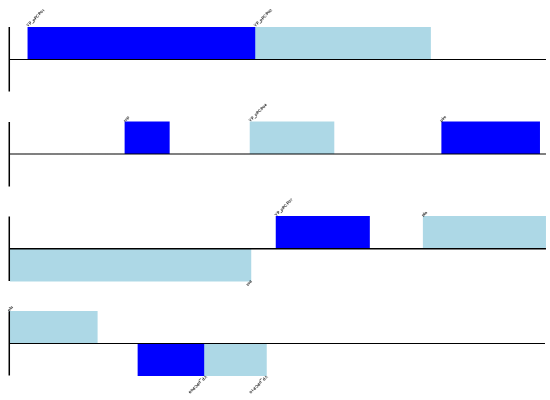
\includegraphics{plasmid_linear.png}

注意,我们将代码中的  \code{fragments} 变量设置为“4”,基因组就会被分为“4”个片段。

如果想要环形图,可以试试以下的代码:
\DUspan{name}{}\DUspan{operator}{}\DUspan{name}{}\DUspan{punctuation}{}\DUspan{name}{}\DUspan{operator}{}\DUspan{literal,string}{}\DUspan{punctuation}{}\DUspan{name}{}\DUspan{operator}{}\DUspan{name,builtin,pseudo}{}\DUspan{punctuation}{}\DUspan{name}{}\DUspan{operator}{}\DUspan{punctuation}{}\DUspan{literal,number,integer}{}\DUspan{operator}{}\DUspan{name}{}\DUspan{punctuation}{}\DUspan{literal,number,integer}{}\DUspan{operator}{}\DUspan{name}{}\DUspan{punctuation}{}\DUspan{name}{}\DUspan{operator}{}\DUspan{literal,number,integer}{}\DUspan{punctuation}{}\DUspan{name}{}\DUspan{operator}{}\DUspan{name,builtin}{}\DUspan{punctuation}{}\DUspan{name}{}\DUspan{punctuation}{}\DUspan{name}{}\DUspan{operator}{}\DUspan{literal,number,float}{}\DUspan{punctuation}{}\DUspan{name}{}\DUspan{operator}{}\DUspan{name}{}\DUspan{punctuation}{}\DUspan{literal,string}{}\DUspan{punctuation}{}\DUspan{literal,string}{}\DUspan{punctuation}{}
\begin{Verbatim}[commandchars=\\\{\}]
\PYG{n}{gd\PYGZus{}diagram}\PYG{o}{.}\PYG{n}{draw}\PYG{p}{(}\PYG{n}{format}\PYG{o}{=}\PYG{l+s}{\PYGZdq{}}\PYG{l+s}{circular}\PYG{l+s}{\PYGZdq{}}\PYG{p}{,} \PYG{n}{circular}\PYG{o}{=}\PYG{n+nb+bp}{True}\PYG{p}{,} \PYG{n}{pagesize}\PYG{o}{=}\PYG{p}{(}\PYG{l+m+mi}{20}\PYG{o}{*}\PYG{n}{cm}\PYG{p}{,}\PYG{l+m+mi}{20}\PYG{o}{*}\PYG{n}{cm}\PYG{p}{)}\PYG{p}{,}
                \PYG{n}{start}\PYG{o}{=}\PYG{l+m+mi}{0}\PYG{p}{,} \PYG{n}{end}\PYG{o}{=}\PYG{n+nb}{len}\PYG{p}{(}\PYG{n}{record}\PYG{p}{)}\PYG{p}{,} \PYG{n}{circle\PYGZus{}core}\PYG{o}{=}\PYG{l+m+mf}{0.7}\PYG{p}{)}
\PYG{n}{gd\PYGZus{}diagram}\PYG{o}{.}\PYG{n}{write}\PYG{p}{(}\PYG{l+s}{\PYGZdq{}}\PYG{l+s}{plasmid\PYGZus{}circular.pdf}\PYG{l+s}{\PYGZdq{}}\PYG{p}{,} \PYG{l+s}{\PYGZdq{}}\PYG{l+s}{PDF}\PYG{l+s}{\PYGZdq{}}\PYG{p}{)}
\end{Verbatim}

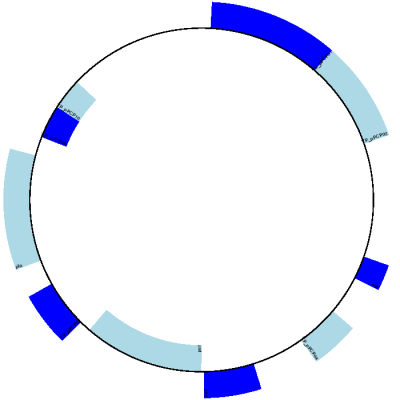
\includegraphics{plasmid_circular.png}

示例图不是非常精彩,但这仅仅是精彩的开始。


\subsection{17.1.4  自下而上的实例}
\label{chr17:id4}
现在,用“自下而上”的方法来创建相同的图形。首先新建不同的对象(可以是任何顺序),然后将其组合。
\DUspan{keyword,namespace}{}\DUspan{name,namespace}{}\DUspan{keyword,namespace}{}\DUspan{name}{}\DUspan{keyword,namespace}{}\DUspan{name,namespace}{}\DUspan{keyword,namespace}{}\DUspan{name}{}\DUspan{keyword,namespace}{}\DUspan{name,namespace}{}\DUspan{keyword,namespace}{}\DUspan{name}{}\DUspan{keyword,namespace}{}\DUspan{name,namespace}{}\DUspan{keyword,namespace}{}\DUspan{name}{}\DUspan{name}{}\DUspan{operator}{}\DUspan{name}{}\DUspan{operator}{}\DUspan{name}{}\DUspan{punctuation}{}\DUspan{literal,string}{}\DUspan{punctuation}{}\DUspan{literal,string}{}\DUspan{punctuation}{}\DUspan{comment}{}\DUspan{name}{}\DUspan{operator}{}\DUspan{name}{}\DUspan{operator}{}\DUspan{name}{}\DUspan{punctuation}{}\DUspan{keyword}{}\DUspan{name}{}\DUspan{operator,word}{}\DUspan{name}{}\DUspan{operator}{}\DUspan{name}{}\DUspan{punctuation}{}\DUspan{keyword}{}\DUspan{name}{}\DUspan{operator}{}\DUspan{name}{}\DUspan{operator}{}\DUspan{literal,string}{}\DUspan{punctuation}{}\DUspan{comment}{}\DUspan{keyword}{}\DUspan{keyword}{}\DUspan{name,builtin}{}\DUspan{punctuation}{}\DUspan{name}{}\DUspan{punctuation}{}\DUspan{operator}{}\DUspan{literal,number,integer}{}\DUspan{operator}{}\DUspan{literal,number,integer}{}\DUspan{punctuation}{}\DUspan{name}{}\DUspan{operator}{}\DUspan{name}{}\DUspan{operator}{}\DUspan{name}{}\DUspan{keyword}{}\DUspan{punctuation}{}\DUspan{name}{}\DUspan{operator}{}\DUspan{name}{}\DUspan{operator}{}\DUspan{name}{}\DUspan{name}{}\DUspan{operator}{}\DUspan{name}{}\DUspan{punctuation}{}\DUspan{name}{}\DUspan{punctuation}{}\DUspan{name}{}\DUspan{operator}{}\DUspan{name}{}\DUspan{punctuation}{}\DUspan{name}{}\DUspan{operator}{}\DUspan{name,builtin,pseudo}{}\DUspan{punctuation}{}\DUspan{comment}{}\DUspan{comment}{}\DUspan{name}{}\DUspan{operator}{}\DUspan{name}{}\DUspan{operator}{}\DUspan{name}{}\DUspan{punctuation}{}\DUspan{name}{}\DUspan{operator}{}\DUspan{literal,string}{}\DUspan{punctuation}{}\DUspan{name}{}\DUspan{operator}{}\DUspan{name}{}\DUspan{operator}{}\DUspan{name}{}\DUspan{punctuation}{}\DUspan{literal,string}{}\DUspan{punctuation}{}\DUspan{comment}{}\DUspan{name}{}\DUspan{operator}{}\DUspan{name}{}\DUspan{punctuation}{}\DUspan{name}{}\DUspan{punctuation}{}\DUspan{name}{}\DUspan{operator}{}\DUspan{name}{}\DUspan{punctuation}{}\DUspan{name}{}\DUspan{punctuation}{}\DUspan{literal,number,integer}{}\DUspan{punctuation}{}
\begin{Verbatim}[commandchars=\\\{\}]
\PYG{k+kn}{from} \PYG{n+nn}{reportlab.lib} \PYG{k+kn}{import} \PYG{n}{colors}
\PYG{k+kn}{from} \PYG{n+nn}{reportlab.lib.units} \PYG{k+kn}{import} \PYG{n}{cm}
\PYG{k+kn}{from} \PYG{n+nn}{Bio.Graphics} \PYG{k+kn}{import} \PYG{n}{GenomeDiagram}
\PYG{k+kn}{from} \PYG{n+nn}{Bio} \PYG{k+kn}{import} \PYG{n}{SeqIO}
\PYG{n}{record} \PYG{o}{=} \PYG{n}{SeqIO}\PYG{o}{.}\PYG{n}{read}\PYG{p}{(}\PYG{l+s}{\PYGZdq{}}\PYG{l+s}{NC\PYGZus{}005816.gb}\PYG{l+s}{\PYGZdq{}}\PYG{p}{,} \PYG{l+s}{\PYGZdq{}}\PYG{l+s}{genbank}\PYG{l+s}{\PYGZdq{}}\PYG{p}{)}

\PYG{c}{\PYGZsh{}Create the feature set and its feature objects,}
\PYG{n}{gd\PYGZus{}feature\PYGZus{}set} \PYG{o}{=} \PYG{n}{GenomeDiagram}\PYG{o}{.}\PYG{n}{FeatureSet}\PYG{p}{(}\PYG{p}{)}
\PYG{k}{for} \PYG{n}{feature} \PYG{o+ow}{in} \PYG{n}{record}\PYG{o}{.}\PYG{n}{features}\PYG{p}{:}
    \PYG{k}{if} \PYG{n}{feature}\PYG{o}{.}\PYG{n}{type} \PYG{o}{!=} \PYG{l+s}{\PYGZdq{}}\PYG{l+s}{gene}\PYG{l+s}{\PYGZdq{}}\PYG{p}{:}
        \PYG{c}{\PYGZsh{}Exclude this feature}
        \PYG{k}{continue}
    \PYG{k}{if} \PYG{n+nb}{len}\PYG{p}{(}\PYG{n}{gd\PYGZus{}feature\PYGZus{}set}\PYG{p}{)} \PYG{o}{\PYGZpc{}} \PYG{l+m+mi}{2} \PYG{o}{==} \PYG{l+m+mi}{0}\PYG{p}{:}
        \PYG{n}{color} \PYG{o}{=} \PYG{n}{colors}\PYG{o}{.}\PYG{n}{blue}
    \PYG{k}{else}\PYG{p}{:}
        \PYG{n}{color} \PYG{o}{=} \PYG{n}{colors}\PYG{o}{.}\PYG{n}{lightblue}
    \PYG{n}{gd\PYGZus{}feature\PYGZus{}set}\PYG{o}{.}\PYG{n}{add\PYGZus{}feature}\PYG{p}{(}\PYG{n}{feature}\PYG{p}{,} \PYG{n}{color}\PYG{o}{=}\PYG{n}{color}\PYG{p}{,} \PYG{n}{label}\PYG{o}{=}\PYG{n+nb+bp}{True}\PYG{p}{)}
\PYG{c}{\PYGZsh{}(this for loop is the same as in the previous example)}

\PYG{c}{\PYGZsh{}Create a track, and a diagram}
\PYG{n}{gd\PYGZus{}track\PYGZus{}for\PYGZus{}features} \PYG{o}{=} \PYG{n}{GenomeDiagram}\PYG{o}{.}\PYG{n}{Track}\PYG{p}{(}\PYG{n}{name}\PYG{o}{=}\PYG{l+s}{\PYGZdq{}}\PYG{l+s}{Annotated Features}\PYG{l+s}{\PYGZdq{}}\PYG{p}{)}
\PYG{n}{gd\PYGZus{}diagram} \PYG{o}{=} \PYG{n}{GenomeDiagram}\PYG{o}{.}\PYG{n}{Diagram}\PYG{p}{(}\PYG{l+s}{\PYGZdq{}}\PYG{l+s}{Yersinia pestis biovar Microtus plasmid pPCP1}\PYG{l+s}{\PYGZdq{}}\PYG{p}{)}

\PYG{c}{\PYGZsh{}Now have to glue the bits together...}
\PYG{n}{gd\PYGZus{}track\PYGZus{}for\PYGZus{}features}\PYG{o}{.}\PYG{n}{add\PYGZus{}set}\PYG{p}{(}\PYG{n}{gd\PYGZus{}feature\PYGZus{}set}\PYG{p}{)}
\PYG{n}{gd\PYGZus{}diagram}\PYG{o}{.}\PYG{n}{add\PYGZus{}track}\PYG{p}{(}\PYG{n}{gd\PYGZus{}track\PYGZus{}for\PYGZus{}features}\PYG{p}{,} \PYG{l+m+mi}{1}\PYG{p}{)}
\end{Verbatim}

同样,利用 \code{draw} 和 \code{write} 方法来创建线形图或者环形图,结果应该完全相同(“draw”和“write”部分的代码见17.1.3)。


\subsection{17.1.5  简单的Feature}
\label{chr17:feature}
以上示例中,创建diagram使用的 \code{SeqRecord} 的 \code{SeqFeature} 对象( 详见 {\hyperref[chr04:sec-seq-features]{\emph{4.3}}} 章节)。如果你不需要 \code{SeqFeature} 对象,只将目标feature定位在坐标轴,仅需要创建minimal
\code{SeqFeature} 对象,方法很简单,代码如下:
\DUspan{keyword,namespace}{}\DUspan{name,namespace}{}\DUspan{keyword,namespace}{}\DUspan{name}{}\DUspan{punctuation}{}\DUspan{name}{}\DUspan{name}{}\DUspan{operator}{}\DUspan{name}{}\DUspan{punctuation}{}\DUspan{name}{}\DUspan{punctuation}{}\DUspan{literal,number,integer}{}\DUspan{punctuation}{}\DUspan{literal,number,integer}{}\DUspan{punctuation}{}\DUspan{name}{}\DUspan{operator}{}\DUspan{literal,number,integer}{}\DUspan{punctuation}{}
\begin{Verbatim}[commandchars=\\\{\}]
\PYG{k+kn}{from} \PYG{n+nn}{Bio.SeqFeature} \PYG{k+kn}{import} \PYG{n}{SeqFeature}\PYG{p}{,} \PYG{n}{FeatureLocation}
\PYG{n}{my\PYGZus{}seq\PYGZus{}feature} \PYG{o}{=} \PYG{n}{SeqFeature}\PYG{p}{(}\PYG{n}{FeatureLocation}\PYG{p}{(}\PYG{l+m+mi}{50}\PYG{p}{,}\PYG{l+m+mi}{100}\PYG{p}{)}\PYG{p}{,}\PYG{n}{strand}\PYG{o}{=}\PYG{o}{+}\PYG{l+m+mi}{1}\PYG{p}{)}
\end{Verbatim}

对于序列来说, \code{+1} 代表正向, \code{-1} 代表反向,  \code{None} 代表两者都有,下面举个简单的示例:
\DUspan{keyword,namespace}{}\DUspan{name,namespace}{}\DUspan{keyword,namespace}{}\DUspan{name}{}\DUspan{punctuation}{}\DUspan{name}{}\DUspan{keyword,namespace}{}\DUspan{name,namespace}{}\DUspan{keyword,namespace}{}\DUspan{name}{}\DUspan{keyword,namespace}{}\DUspan{name,namespace}{}\DUspan{keyword,namespace}{}\DUspan{name}{}\DUspan{name}{}\DUspan{operator}{}\DUspan{name}{}\DUspan{operator}{}\DUspan{name}{}\DUspan{punctuation}{}\DUspan{literal,string}{}\DUspan{punctuation}{}\DUspan{name}{}\DUspan{operator}{}\DUspan{name}{}\DUspan{operator}{}\DUspan{name}{}\DUspan{punctuation}{}\DUspan{literal,number,integer}{}\DUspan{punctuation}{}\DUspan{name}{}\DUspan{operator}{}\DUspan{name,builtin,pseudo}{}\DUspan{punctuation}{}\DUspan{name}{}\DUspan{operator}{}\DUspan{name}{}\DUspan{operator}{}\DUspan{name}{}\DUspan{punctuation}{}\DUspan{comment}{}\DUspan{name}{}\DUspan{operator}{}\DUspan{name}{}\DUspan{punctuation}{}\DUspan{name}{}\DUspan{punctuation}{}\DUspan{literal,number,integer}{}\DUspan{punctuation}{}\DUspan{literal,number,integer}{}\DUspan{punctuation}{}\DUspan{name}{}\DUspan{operator}{}\DUspan{literal,number,integer}{}\DUspan{punctuation}{}\DUspan{name}{}\DUspan{operator}{}\DUspan{name}{}\DUspan{punctuation}{}\DUspan{name}{}\DUspan{punctuation}{}\DUspan{name}{}\DUspan{operator}{}\DUspan{literal,string}{}\DUspan{punctuation}{}\DUspan{name}{}\DUspan{operator}{}\DUspan{name,builtin,pseudo}{}\DUspan{punctuation}{}\DUspan{name}{}\DUspan{operator}{}\DUspan{name}{}\DUspan{punctuation}{}\DUspan{name}{}\DUspan{punctuation}{}\DUspan{literal,number,integer}{}\DUspan{punctuation}{}\DUspan{literal,number,integer}{}\DUspan{punctuation}{}\DUspan{name}{}\DUspan{operator}{}\DUspan{name,builtin,pseudo}{}\DUspan{punctuation}{}\DUspan{name}{}\DUspan{operator}{}\DUspan{name}{}\DUspan{punctuation}{}\DUspan{name}{}\DUspan{punctuation}{}\DUspan{name}{}\DUspan{operator}{}\DUspan{literal,string}{}\DUspan{punctuation}{}\DUspan{name}{}\DUspan{operator}{}\DUspan{name,builtin,pseudo}{}\DUspan{punctuation}{}\DUspan{name}{}\DUspan{operator}{}\DUspan{name}{}\DUspan{punctuation}{}\DUspan{name}{}\DUspan{punctuation}{}\DUspan{literal,number,integer}{}\DUspan{punctuation}{}\DUspan{literal,number,integer}{}\DUspan{punctuation}{}\DUspan{name}{}\DUspan{operator}{}\DUspan{literal,number,integer}{}\DUspan{punctuation}{}\DUspan{name}{}\DUspan{operator}{}\DUspan{name}{}\DUspan{punctuation}{}\DUspan{name}{}\DUspan{punctuation}{}\DUspan{name}{}\DUspan{operator}{}\DUspan{literal,string}{}\DUspan{punctuation}{}\DUspan{name}{}\DUspan{operator}{}\DUspan{name,builtin,pseudo}{}\DUspan{punctuation}{}\DUspan{name}{}\DUspan{operator}{}\DUspan{name}{}\DUspan{punctuation}{}\DUspan{name}{}\DUspan{operator}{}\DUspan{literal,string}{}\DUspan{punctuation}{}\DUspan{name}{}\DUspan{operator}{}\DUspan{punctuation}{}\DUspan{literal,number,integer}{}\DUspan{operator}{}\DUspan{name}{}\DUspan{punctuation}{}\DUspan{literal,number,integer}{}\DUspan{operator}{}\DUspan{name}{}\DUspan{punctuation}{}\DUspan{name}{}\DUspan{operator}{}\DUspan{literal,number,integer}{}\DUspan{punctuation}{}\DUspan{name}{}\DUspan{operator}{}\DUspan{literal,number,integer}{}\DUspan{punctuation}{}\DUspan{name}{}\DUspan{operator}{}\DUspan{literal,number,integer}{}\DUspan{punctuation}{}\DUspan{name}{}\DUspan{operator}{}\DUspan{name}{}\DUspan{punctuation}{}\DUspan{literal,string}{}\DUspan{punctuation}{}\DUspan{literal,string}{}\DUspan{punctuation}{}
\begin{Verbatim}[commandchars=\\\{\}]
\PYG{k+kn}{from} \PYG{n+nn}{Bio.SeqFeature} \PYG{k+kn}{import} \PYG{n}{SeqFeature}\PYG{p}{,} \PYG{n}{FeatureLocation}
\PYG{k+kn}{from} \PYG{n+nn}{Bio.Graphics} \PYG{k+kn}{import} \PYG{n}{GenomeDiagram}
\PYG{k+kn}{from} \PYG{n+nn}{reportlab.lib.units} \PYG{k+kn}{import} \PYG{n}{cm}

\PYG{n}{gdd} \PYG{o}{=} \PYG{n}{GenomeDiagram}\PYG{o}{.}\PYG{n}{Diagram}\PYG{p}{(}\PYG{l+s}{\PYGZsq{}}\PYG{l+s}{Test Diagram}\PYG{l+s}{\PYGZsq{}}\PYG{p}{)}
\PYG{n}{gdt\PYGZus{}features} \PYG{o}{=} \PYG{n}{gdd}\PYG{o}{.}\PYG{n}{new\PYGZus{}track}\PYG{p}{(}\PYG{l+m+mi}{1}\PYG{p}{,} \PYG{n}{greytrack}\PYG{o}{=}\PYG{n+nb+bp}{False}\PYG{p}{)}
\PYG{n}{gds\PYGZus{}features} \PYG{o}{=} \PYG{n}{gdt\PYGZus{}features}\PYG{o}{.}\PYG{n}{new\PYGZus{}set}\PYG{p}{(}\PYG{p}{)}

\PYG{c}{\PYGZsh{}Add three features to show the strand options,}
\PYG{n}{feature} \PYG{o}{=} \PYG{n}{SeqFeature}\PYG{p}{(}\PYG{n}{FeatureLocation}\PYG{p}{(}\PYG{l+m+mi}{25}\PYG{p}{,} \PYG{l+m+mi}{125}\PYG{p}{)}\PYG{p}{,} \PYG{n}{strand}\PYG{o}{=}\PYG{o}{+}\PYG{l+m+mi}{1}\PYG{p}{)}
\PYG{n}{gds\PYGZus{}features}\PYG{o}{.}\PYG{n}{add\PYGZus{}feature}\PYG{p}{(}\PYG{n}{feature}\PYG{p}{,} \PYG{n}{name}\PYG{o}{=}\PYG{l+s}{\PYGZdq{}}\PYG{l+s}{Forward}\PYG{l+s}{\PYGZdq{}}\PYG{p}{,} \PYG{n}{label}\PYG{o}{=}\PYG{n+nb+bp}{True}\PYG{p}{)}
\PYG{n}{feature} \PYG{o}{=} \PYG{n}{SeqFeature}\PYG{p}{(}\PYG{n}{FeatureLocation}\PYG{p}{(}\PYG{l+m+mi}{150}\PYG{p}{,} \PYG{l+m+mi}{250}\PYG{p}{)}\PYG{p}{,} \PYG{n}{strand}\PYG{o}{=}\PYG{n+nb+bp}{None}\PYG{p}{)}
\PYG{n}{gds\PYGZus{}features}\PYG{o}{.}\PYG{n}{add\PYGZus{}feature}\PYG{p}{(}\PYG{n}{feature}\PYG{p}{,} \PYG{n}{name}\PYG{o}{=}\PYG{l+s}{\PYGZdq{}}\PYG{l+s}{Strandless}\PYG{l+s}{\PYGZdq{}}\PYG{p}{,} \PYG{n}{label}\PYG{o}{=}\PYG{n+nb+bp}{True}\PYG{p}{)}
\PYG{n}{feature} \PYG{o}{=} \PYG{n}{SeqFeature}\PYG{p}{(}\PYG{n}{FeatureLocation}\PYG{p}{(}\PYG{l+m+mi}{275}\PYG{p}{,} \PYG{l+m+mi}{375}\PYG{p}{)}\PYG{p}{,} \PYG{n}{strand}\PYG{o}{=}\PYG{o}{\PYGZhy{}}\PYG{l+m+mi}{1}\PYG{p}{)}
\PYG{n}{gds\PYGZus{}features}\PYG{o}{.}\PYG{n}{add\PYGZus{}feature}\PYG{p}{(}\PYG{n}{feature}\PYG{p}{,} \PYG{n}{name}\PYG{o}{=}\PYG{l+s}{\PYGZdq{}}\PYG{l+s}{Reverse}\PYG{l+s}{\PYGZdq{}}\PYG{p}{,} \PYG{n}{label}\PYG{o}{=}\PYG{n+nb+bp}{True}\PYG{p}{)}

\PYG{n}{gdd}\PYG{o}{.}\PYG{n}{draw}\PYG{p}{(}\PYG{n}{format}\PYG{o}{=}\PYG{l+s}{\PYGZsq{}}\PYG{l+s}{linear}\PYG{l+s}{\PYGZsq{}}\PYG{p}{,} \PYG{n}{pagesize}\PYG{o}{=}\PYG{p}{(}\PYG{l+m+mi}{15}\PYG{o}{*}\PYG{n}{cm}\PYG{p}{,}\PYG{l+m+mi}{4}\PYG{o}{*}\PYG{n}{cm}\PYG{p}{)}\PYG{p}{,} \PYG{n}{fragments}\PYG{o}{=}\PYG{l+m+mi}{1}\PYG{p}{,}
         \PYG{n}{start}\PYG{o}{=}\PYG{l+m+mi}{0}\PYG{p}{,} \PYG{n}{end}\PYG{o}{=}\PYG{l+m+mi}{400}\PYG{p}{)}
\PYG{n}{gdd}\PYG{o}{.}\PYG{n}{write}\PYG{p}{(}\PYG{l+s}{\PYGZdq{}}\PYG{l+s}{GD\PYGZus{}labels\PYGZus{}default.pdf}\PYG{l+s}{\PYGZdq{}}\PYG{p}{,} \PYG{l+s}{\PYGZdq{}}\PYG{l+s}{pdf}\PYG{l+s}{\PYGZdq{}}\PYG{p}{)}
\end{Verbatim}

图形示例结果请见下一节图中的第一个图,缺省的feature为浅绿色。

注意,这里用 \code{name} 参数作为feature的“说明文本”(caption text)。下文将会讲述更多细节。


\subsection{17.1.6  Feature说明}
\label{chr17:id5}
下面代码中, \code{feature} 作为 \code{SeqFeature} 的对象添加到diagram。
\DUspan{name}{}\DUspan{operator}{}\DUspan{name}{}\DUspan{punctuation}{}\DUspan{name}{}\DUspan{punctuation}{}\DUspan{name}{}\DUspan{operator}{}\DUspan{name}{}\DUspan{punctuation}{}\DUspan{name}{}\DUspan{operator}{}\DUspan{name,builtin,pseudo}{}\DUspan{punctuation}{}
\begin{Verbatim}[commandchars=\\\{\}]
\PYG{n}{gd\PYGZus{}feature\PYGZus{}set}\PYG{o}{.}\PYG{n}{add\PYGZus{}feature}\PYG{p}{(}\PYG{n}{feature}\PYG{p}{,} \PYG{n}{color}\PYG{o}{=}\PYG{n}{color}\PYG{p}{,} \PYG{n}{label}\PYG{o}{=}\PYG{n+nb+bp}{True}\PYG{p}{)}
\end{Verbatim}

前面的示例用 \code{SeqFeature} 的注释为feature做了恰当的文字说明。 \code{SeqFeature} 对象的限定符(qualifiers dictionary)缺省值是: \code{gene}, \code{label}, \code{name}, \code{locus\_tag}, 和 \code{product} 。简单地说,你可以定义一个名称:
\DUspan{name}{}\DUspan{operator}{}\DUspan{name}{}\DUspan{punctuation}{}\DUspan{name}{}\DUspan{punctuation}{}\DUspan{name}{}\DUspan{operator}{}\DUspan{name}{}\DUspan{punctuation}{}\DUspan{name}{}\DUspan{operator}{}\DUspan{name,builtin,pseudo}{}\DUspan{punctuation}{}\DUspan{name}{}\DUspan{operator}{}\DUspan{literal,string}{}\DUspan{punctuation}{}
\begin{Verbatim}[commandchars=\\\{\}]
\PYG{n}{gd\PYGZus{}feature\PYGZus{}set}\PYG{o}{.}\PYG{n}{add\PYGZus{}feature}\PYG{p}{(}\PYG{n}{feature}\PYG{p}{,} \PYG{n}{color}\PYG{o}{=}\PYG{n}{color}\PYG{p}{,} \PYG{n}{label}\PYG{o}{=}\PYG{n+nb+bp}{True}\PYG{p}{,} \PYG{n}{name}\PYG{o}{=}\PYG{l+s}{\PYGZdq{}}\PYG{l+s}{My Gene}\PYG{l+s}{\PYGZdq{}}\PYG{p}{)}
\end{Verbatim}

每个feature标签的说明文本可以设置字体、位置和方向。说明文本默认的位置在图形符号(sigil)的左边,可选择在中间或者右边,线形图中文本的默认方向是45°旋转。
\DUspan{comment}{}\DUspan{name}{}\DUspan{operator}{}\DUspan{name}{}\DUspan{punctuation}{}\DUspan{name}{}\DUspan{punctuation}{}\DUspan{name}{}\DUspan{operator}{}\DUspan{name,builtin,pseudo}{}\DUspan{punctuation}{}\DUspan{name}{}\DUspan{operator}{}\DUspan{literal,string}{}\DUspan{punctuation}{}\DUspan{name}{}\DUspan{operator}{}\DUspan{literal,number,integer}{}\DUspan{punctuation}{}\DUspan{name}{}\DUspan{operator}{}\DUspan{literal,number,integer}{}\DUspan{punctuation}{}\DUspan{comment}{}\DUspan{name}{}\DUspan{operator}{}\DUspan{name}{}\DUspan{punctuation}{}\DUspan{name}{}\DUspan{punctuation}{}\DUspan{name}{}\DUspan{operator}{}\DUspan{name,builtin,pseudo}{}\DUspan{punctuation}{}\DUspan{name}{}\DUspan{operator}{}\DUspan{literal,string}{}\DUspan{punctuation}{}\DUspan{name}{}\DUspan{operator}{}\DUspan{literal,string}{}\DUspan{punctuation}{}\DUspan{name}{}\DUspan{operator}{}\DUspan{literal,number,integer}{}\DUspan{punctuation}{}\DUspan{name}{}\DUspan{operator}{}\DUspan{literal,number,integer}{}\DUspan{punctuation}{}\DUspan{comment}{}\DUspan{name}{}\DUspan{operator}{}\DUspan{name}{}\DUspan{punctuation}{}\DUspan{name}{}\DUspan{punctuation}{}\DUspan{name}{}\DUspan{operator}{}\DUspan{name,builtin,pseudo}{}\DUspan{punctuation}{}\DUspan{name}{}\DUspan{operator}{}\DUspan{literal,string}{}\DUspan{punctuation}{}\DUspan{name}{}\DUspan{operator}{}\DUspan{literal,string}{}\DUspan{punctuation}{}\DUspan{name}{}\DUspan{operator}{}\DUspan{literal,number,integer}{}\DUspan{punctuation}{}\DUspan{name}{}\DUspan{operator}{}\DUspan{literal,number,integer}{}\DUspan{punctuation}{}
\begin{Verbatim}[commandchars=\\\{\}]
\PYG{c}{\PYGZsh{}Large font, parallel with the track}
\PYG{n}{gd\PYGZus{}feature\PYGZus{}set}\PYG{o}{.}\PYG{n}{add\PYGZus{}feature}\PYG{p}{(}\PYG{n}{feature}\PYG{p}{,} \PYG{n}{label}\PYG{o}{=}\PYG{n+nb+bp}{True}\PYG{p}{,} \PYG{n}{color}\PYG{o}{=}\PYG{l+s}{\PYGZdq{}}\PYG{l+s}{green}\PYG{l+s}{\PYGZdq{}}\PYG{p}{,}
                           \PYG{n}{label\PYGZus{}size}\PYG{o}{=}\PYG{l+m+mi}{25}\PYG{p}{,} \PYG{n}{label\PYGZus{}angle}\PYG{o}{=}\PYG{l+m+mi}{0}\PYG{p}{)}

\PYG{c}{\PYGZsh{}Very small font, perpendicular to the track (towards it)}
\PYG{n}{gd\PYGZus{}feature\PYGZus{}set}\PYG{o}{.}\PYG{n}{add\PYGZus{}feature}\PYG{p}{(}\PYG{n}{feature}\PYG{p}{,} \PYG{n}{label}\PYG{o}{=}\PYG{n+nb+bp}{True}\PYG{p}{,} \PYG{n}{color}\PYG{o}{=}\PYG{l+s}{\PYGZdq{}}\PYG{l+s}{purple}\PYG{l+s}{\PYGZdq{}}\PYG{p}{,}
                           \PYG{n}{label\PYGZus{}position}\PYG{o}{=}\PYG{l+s}{\PYGZdq{}}\PYG{l+s}{end}\PYG{l+s}{\PYGZdq{}}\PYG{p}{,}
                           \PYG{n}{label\PYGZus{}size}\PYG{o}{=}\PYG{l+m+mi}{4}\PYG{p}{,} \PYG{n}{label\PYGZus{}angle}\PYG{o}{=}\PYG{l+m+mi}{90}\PYG{p}{)}

\PYG{c}{\PYGZsh{}Small font, perpendicular to the track (away from it)}
\PYG{n}{gd\PYGZus{}feature\PYGZus{}set}\PYG{o}{.}\PYG{n}{add\PYGZus{}feature}\PYG{p}{(}\PYG{n}{feature}\PYG{p}{,} \PYG{n}{label}\PYG{o}{=}\PYG{n+nb+bp}{True}\PYG{p}{,} \PYG{n}{color}\PYG{o}{=}\PYG{l+s}{\PYGZdq{}}\PYG{l+s}{blue}\PYG{l+s}{\PYGZdq{}}\PYG{p}{,}
                           \PYG{n}{label\PYGZus{}position}\PYG{o}{=}\PYG{l+s}{\PYGZdq{}}\PYG{l+s}{middle}\PYG{l+s}{\PYGZdq{}}\PYG{p}{,}
                           \PYG{n}{label\PYGZus{}size}\PYG{o}{=}\PYG{l+m+mi}{6}\PYG{p}{,} \PYG{n}{label\PYGZus{}angle}\PYG{o}{=}\PYG{o}{\PYGZhy{}}\PYG{l+m+mi}{90}\PYG{p}{)}
\end{Verbatim}

用前面示例的代码将这三个片段组合之后应该可以得到如下的结果:

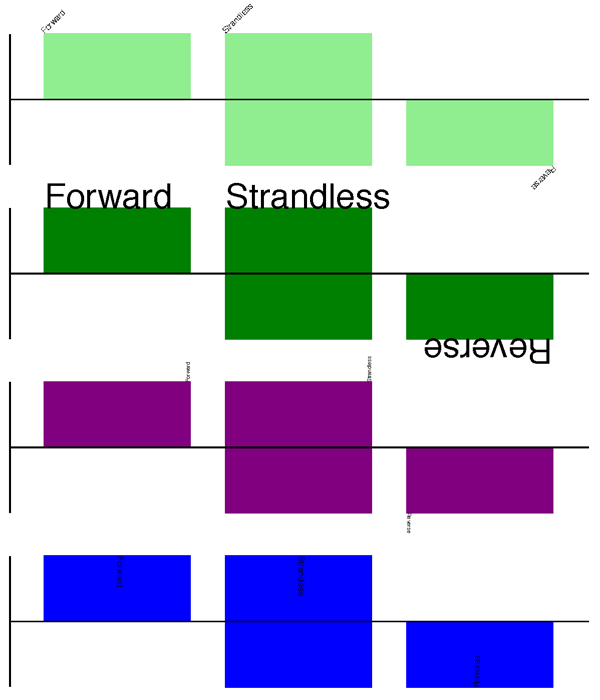
\includegraphics{GD_sigil_labels.png}

除此之外,还可以设置“label\_color”来调节标签的颜色(第 {\hyperref[chr17:sec-gd-nice-example]{\emph{17.1.9}}} 节也将用到这一步),这里没有进行演示。

示例中默认的字体很小,这是比较明智的,因为通常我们会把许多Feature同时展示,而不像这里只展示了几个比较大的feature。


\subsection{17.1.7  表示Feature的图形符号}
\label{chr17:id6}
以上示例中Feature的图形符号(sigil)默认是一个方框(plain box),GenomeDiagram第一版中只有这一选项,后来GenomeDiagram被整合到Biopython1.50时,新增了箭头状的图形符号(sigil)。
\DUspan{comment}{}\DUspan{name}{}\DUspan{operator}{}\DUspan{name}{}\DUspan{punctuation}{}\DUspan{name}{}\DUspan{punctuation}{}\DUspan{comment}{}\DUspan{name}{}\DUspan{operator}{}\DUspan{name}{}\DUspan{punctuation}{}\DUspan{name}{}\DUspan{punctuation}{}\DUspan{name}{}\DUspan{operator}{}\DUspan{literal,string}{}\DUspan{punctuation}{}\DUspan{comment}{}\DUspan{name}{}\DUspan{operator}{}\DUspan{name}{}\DUspan{punctuation}{}\DUspan{name}{}\DUspan{punctuation}{}\DUspan{name}{}\DUspan{operator}{}\DUspan{literal,string}{}\DUspan{punctuation}{}
\begin{Verbatim}[commandchars=\\\{\}]
\PYG{c}{\PYGZsh{}Default uses a BOX sigil}
\PYG{n}{gd\PYGZus{}feature\PYGZus{}set}\PYG{o}{.}\PYG{n}{add\PYGZus{}feature}\PYG{p}{(}\PYG{n}{feature}\PYG{p}{)}

\PYG{c}{\PYGZsh{}You can make this explicit:}
\PYG{n}{gd\PYGZus{}feature\PYGZus{}set}\PYG{o}{.}\PYG{n}{add\PYGZus{}feature}\PYG{p}{(}\PYG{n}{feature}\PYG{p}{,} \PYG{n}{sigil}\PYG{o}{=}\PYG{l+s}{\PYGZdq{}}\PYG{l+s}{BOX}\PYG{l+s}{\PYGZdq{}}\PYG{p}{)}

\PYG{c}{\PYGZsh{}Or opt for an arrow:}
\PYG{n}{gd\PYGZus{}feature\PYGZus{}set}\PYG{o}{.}\PYG{n}{add\PYGZus{}feature}\PYG{p}{(}\PYG{n}{feature}\PYG{p}{,} \PYG{n}{sigil}\PYG{o}{=}\PYG{l+s}{\PYGZdq{}}\PYG{l+s}{ARROW}\PYG{l+s}{\PYGZdq{}}\PYG{p}{)}
\end{Verbatim}

Biopython 1.61又新增3个图形形状(sigil)。
\DUspan{comment}{}\DUspan{name}{}\DUspan{operator}{}\DUspan{name}{}\DUspan{punctuation}{}\DUspan{name}{}\DUspan{punctuation}{}\DUspan{name}{}\DUspan{operator}{}\DUspan{literal,string}{}\DUspan{punctuation}{}\DUspan{comment}{}\DUspan{name}{}\DUspan{operator}{}\DUspan{name}{}\DUspan{punctuation}{}\DUspan{name}{}\DUspan{punctuation}{}\DUspan{name}{}\DUspan{operator}{}\DUspan{literal,string}{}\DUspan{punctuation}{}\DUspan{comment}{}\DUspan{name}{}\DUspan{operator}{}\DUspan{name}{}\DUspan{punctuation}{}\DUspan{name}{}\DUspan{punctuation}{}\DUspan{name}{}\DUspan{operator}{}\DUspan{literal,string}{}\DUspan{punctuation}{}
\begin{Verbatim}[commandchars=\\\{\}]
\PYG{c}{\PYGZsh{}Box with corners cut off (making it an octagon)}
\PYG{n}{gd\PYGZus{}feature\PYGZus{}set}\PYG{o}{.}\PYG{n}{add\PYGZus{}feature}\PYG{p}{(}\PYG{n}{feature}\PYG{p}{,} \PYG{n}{sigil}\PYG{o}{=}\PYG{l+s}{\PYGZdq{}}\PYG{l+s}{OCTO}\PYG{l+s}{\PYGZdq{}}\PYG{p}{)}

\PYG{c}{\PYGZsh{}Box with jagged edges (useful for showing breaks in contains)}
\PYG{n}{gd\PYGZus{}feature\PYGZus{}set}\PYG{o}{.}\PYG{n}{add\PYGZus{}feature}\PYG{p}{(}\PYG{n}{feature}\PYG{p}{,} \PYG{n}{sigil}\PYG{o}{=}\PYG{l+s}{\PYGZdq{}}\PYG{l+s}{JAGGY}\PYG{l+s}{\PYGZdq{}}\PYG{p}{)}

\PYG{c}{\PYGZsh{}Arrow which spans the axis with strand used only for direction}
\PYG{n}{gd\PYGZus{}feature\PYGZus{}set}\PYG{o}{.}\PYG{n}{add\PYGZus{}feature}\PYG{p}{(}\PYG{n}{feature}\PYG{p}{,} \PYG{n}{sigil}\PYG{o}{=}\PYG{l+s}{\PYGZdq{}}\PYG{l+s}{BIGARROW}\PYG{l+s}{\PYGZdq{}}\PYG{p}{)}
\end{Verbatim}

下面就是这些新增的图形形状(sigil),多数的图形形状都在边界框(bounding box)内部,在坐标轴的上/下位置代表序列(Strand)方向的正/反向,或者上下跨越坐标轴,高度是其他图形形状的两倍。“BIGARROW”有所不同,它总是跨越坐标轴,方向由feature的序列决定。

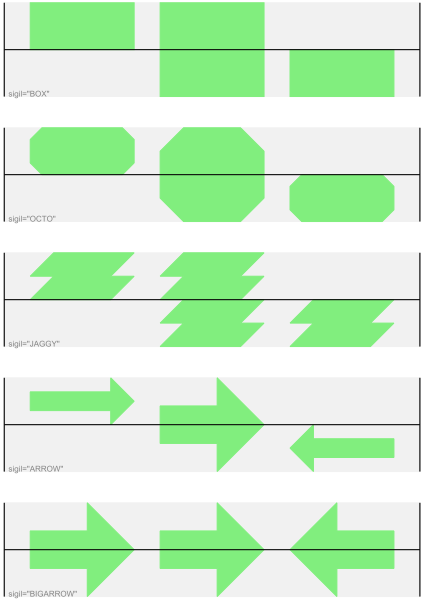
\includegraphics{GD_sigils.png}


\subsection{17.1.8 箭头形状}
\label{chr17:id7}
上一部分我们简单引出了箭头形状。还有两个选项可以对箭头形状进行设置:首先根据边界框的高度比例来设置箭杆宽度。
\DUspan{comment}{}\DUspan{name}{}\DUspan{operator}{}\DUspan{name}{}\DUspan{punctuation}{}\DUspan{name}{}\DUspan{punctuation}{}\DUspan{name}{}\DUspan{operator}{}\DUspan{literal,string}{}\DUspan{punctuation}{}\DUspan{name}{}\DUspan{operator}{}\DUspan{literal,string}{}\DUspan{punctuation}{}\DUspan{name}{}\DUspan{operator}{}\DUspan{literal,number,float}{}\DUspan{punctuation}{}\DUspan{comment}{}\DUspan{name}{}\DUspan{operator}{}\DUspan{name}{}\DUspan{punctuation}{}\DUspan{name}{}\DUspan{punctuation}{}\DUspan{name}{}\DUspan{operator}{}\DUspan{literal,string}{}\DUspan{punctuation}{}\DUspan{name}{}\DUspan{operator}{}\DUspan{literal,string}{}\DUspan{punctuation}{}\DUspan{name}{}\DUspan{operator}{}\DUspan{literal,number,float}{}\DUspan{punctuation}{}\DUspan{comment}{}\DUspan{name}{}\DUspan{operator}{}\DUspan{name}{}\DUspan{punctuation}{}\DUspan{name}{}\DUspan{punctuation}{}\DUspan{name}{}\DUspan{operator}{}\DUspan{literal,string}{}\DUspan{punctuation}{}\DUspan{name}{}\DUspan{operator}{}\DUspan{literal,string}{}\DUspan{punctuation}{}\DUspan{name}{}\DUspan{operator}{}\DUspan{literal,number,float}{}\DUspan{punctuation}{}
\begin{Verbatim}[commandchars=\\\{\}]
\PYG{c}{\PYGZsh{}Full height shafts, giving pointed boxes:}
\PYG{n}{gd\PYGZus{}feature\PYGZus{}set}\PYG{o}{.}\PYG{n}{add\PYGZus{}feature}\PYG{p}{(}\PYG{n}{feature}\PYG{p}{,} \PYG{n}{sigil}\PYG{o}{=}\PYG{l+s}{\PYGZdq{}}\PYG{l+s}{ARROW}\PYG{l+s}{\PYGZdq{}}\PYG{p}{,} \PYG{n}{color}\PYG{o}{=}\PYG{l+s}{\PYGZdq{}}\PYG{l+s}{brown}\PYG{l+s}{\PYGZdq{}}\PYG{p}{,}
                           \PYG{n}{arrowshaft\PYGZus{}height}\PYG{o}{=}\PYG{l+m+mf}{1.0}\PYG{p}{)}
\PYG{c}{\PYGZsh{}Or, thin shafts:}
\PYG{n}{gd\PYGZus{}feature\PYGZus{}set}\PYG{o}{.}\PYG{n}{add\PYGZus{}feature}\PYG{p}{(}\PYG{n}{feature}\PYG{p}{,} \PYG{n}{sigil}\PYG{o}{=}\PYG{l+s}{\PYGZdq{}}\PYG{l+s}{ARROW}\PYG{l+s}{\PYGZdq{}}\PYG{p}{,} \PYG{n}{color}\PYG{o}{=}\PYG{l+s}{\PYGZdq{}}\PYG{l+s}{teal}\PYG{l+s}{\PYGZdq{}}\PYG{p}{,}
                           \PYG{n}{arrowshaft\PYGZus{}height}\PYG{o}{=}\PYG{l+m+mf}{0.2}\PYG{p}{)}
\PYG{c}{\PYGZsh{}Or, very thin shafts:}
\PYG{n}{gd\PYGZus{}feature\PYGZus{}set}\PYG{o}{.}\PYG{n}{add\PYGZus{}feature}\PYG{p}{(}\PYG{n}{feature}\PYG{p}{,} \PYG{n}{sigil}\PYG{o}{=}\PYG{l+s}{\PYGZdq{}}\PYG{l+s}{ARROW}\PYG{l+s}{\PYGZdq{}}\PYG{p}{,} \PYG{n}{color}\PYG{o}{=}\PYG{l+s}{\PYGZdq{}}\PYG{l+s}{darkgreen}\PYG{l+s}{\PYGZdq{}}\PYG{p}{,}
                           \PYG{n}{arrowshaft\PYGZus{}height}\PYG{o}{=}\PYG{l+m+mf}{0.1}\PYG{p}{)}
\end{Verbatim}

结果见下图:

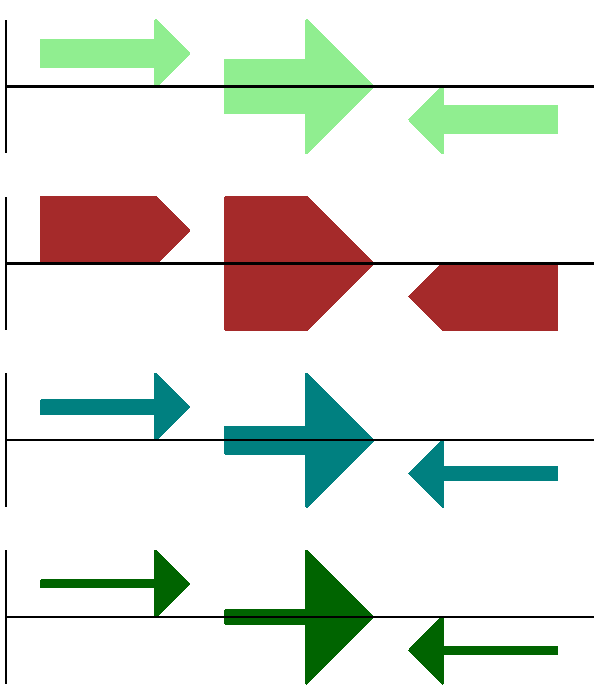
\includegraphics{GD_sigil_arrow_shafts.png}

其次,根据边界框的高度比例设置箭头长度(默认为0.5或50\%):
\DUspan{comment}{}\DUspan{name}{}\DUspan{operator}{}\DUspan{name}{}\DUspan{punctuation}{}\DUspan{name}{}\DUspan{punctuation}{}\DUspan{name}{}\DUspan{operator}{}\DUspan{literal,string}{}\DUspan{punctuation}{}\DUspan{name}{}\DUspan{operator}{}\DUspan{literal,string}{}\DUspan{punctuation}{}\DUspan{name}{}\DUspan{operator}{}\DUspan{literal,number,float}{}\DUspan{punctuation}{}\DUspan{comment}{}\DUspan{name}{}\DUspan{operator}{}\DUspan{name}{}\DUspan{punctuation}{}\DUspan{name}{}\DUspan{punctuation}{}\DUspan{name}{}\DUspan{operator}{}\DUspan{literal,string}{}\DUspan{punctuation}{}\DUspan{name}{}\DUspan{operator}{}\DUspan{literal,string}{}\DUspan{punctuation}{}\DUspan{name}{}\DUspan{operator}{}\DUspan{literal,number,integer}{}\DUspan{punctuation}{}\DUspan{comment}{}\DUspan{name}{}\DUspan{operator}{}\DUspan{name}{}\DUspan{punctuation}{}\DUspan{name}{}\DUspan{punctuation}{}\DUspan{name}{}\DUspan{operator}{}\DUspan{literal,string}{}\DUspan{punctuation}{}\DUspan{name}{}\DUspan{operator}{}\DUspan{literal,string}{}\DUspan{punctuation}{}\DUspan{name}{}\DUspan{operator}{}\DUspan{literal,number,integer}{}\DUspan{punctuation}{}
\begin{Verbatim}[commandchars=\\\{\}]
\PYG{c}{\PYGZsh{}Short arrow heads:}
\PYG{n}{gd\PYGZus{}feature\PYGZus{}set}\PYG{o}{.}\PYG{n}{add\PYGZus{}feature}\PYG{p}{(}\PYG{n}{feature}\PYG{p}{,} \PYG{n}{sigil}\PYG{o}{=}\PYG{l+s}{\PYGZdq{}}\PYG{l+s}{ARROW}\PYG{l+s}{\PYGZdq{}}\PYG{p}{,} \PYG{n}{color}\PYG{o}{=}\PYG{l+s}{\PYGZdq{}}\PYG{l+s}{blue}\PYG{l+s}{\PYGZdq{}}\PYG{p}{,}
                           \PYG{n}{arrowhead\PYGZus{}length}\PYG{o}{=}\PYG{l+m+mf}{0.25}\PYG{p}{)}
\PYG{c}{\PYGZsh{}Or, longer arrow heads:}
\PYG{n}{gd\PYGZus{}feature\PYGZus{}set}\PYG{o}{.}\PYG{n}{add\PYGZus{}feature}\PYG{p}{(}\PYG{n}{feature}\PYG{p}{,} \PYG{n}{sigil}\PYG{o}{=}\PYG{l+s}{\PYGZdq{}}\PYG{l+s}{ARROW}\PYG{l+s}{\PYGZdq{}}\PYG{p}{,} \PYG{n}{color}\PYG{o}{=}\PYG{l+s}{\PYGZdq{}}\PYG{l+s}{orange}\PYG{l+s}{\PYGZdq{}}\PYG{p}{,}
                           \PYG{n}{arrowhead\PYGZus{}length}\PYG{o}{=}\PYG{l+m+mi}{1}\PYG{p}{)}
\PYG{c}{\PYGZsh{}Or, very very long arrow heads (i.e. all head, no shaft, so triangles):}
\PYG{n}{gd\PYGZus{}feature\PYGZus{}set}\PYG{o}{.}\PYG{n}{add\PYGZus{}feature}\PYG{p}{(}\PYG{n}{feature}\PYG{p}{,} \PYG{n}{sigil}\PYG{o}{=}\PYG{l+s}{\PYGZdq{}}\PYG{l+s}{ARROW}\PYG{l+s}{\PYGZdq{}}\PYG{p}{,} \PYG{n}{color}\PYG{o}{=}\PYG{l+s}{\PYGZdq{}}\PYG{l+s}{red}\PYG{l+s}{\PYGZdq{}}\PYG{p}{,}
                           \PYG{n}{arrowhead\PYGZus{}length}\PYG{o}{=}\PYG{l+m+mi}{10000}\PYG{p}{)}
\end{Verbatim}

结果见下图:

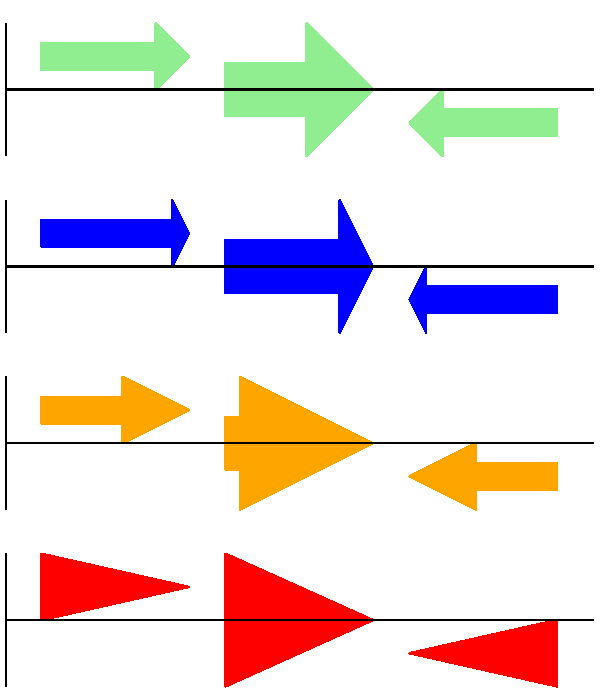
\includegraphics{GD_sigil_arrow_heads.png}

Biopython1.61新增 \code{BIGARROW} 箭头形状,它经常跨越坐标轴,箭头指向”左边“代表”反向“,指向”右边“代表”正向“。
\DUspan{comment}{}\DUspan{name}{}\DUspan{operator}{}\DUspan{name}{}\DUspan{punctuation}{}\DUspan{name}{}\DUspan{punctuation}{}\DUspan{name}{}\DUspan{operator}{}\DUspan{literal,string}{}\DUspan{punctuation}{}
\begin{Verbatim}[commandchars=\\\{\}]
\PYG{c}{\PYGZsh{}A large arrow straddling the axis:}
\PYG{n}{gd\PYGZus{}feature\PYGZus{}set}\PYG{o}{.}\PYG{n}{add\PYGZus{}feature}\PYG{p}{(}\PYG{n}{feature}\PYG{p}{,} \PYG{n}{sigil}\PYG{o}{=}\PYG{l+s}{\PYGZdq{}}\PYG{l+s}{BIGARROW}\PYG{l+s}{\PYGZdq{}}\PYG{p}{)}
\end{Verbatim}

上述 \code{ARROW} 形状中的箭杆和箭头设置选项都适用于 \code{BIGARROW} 。


\subsection{17.1.9 完美示例}
\label{chr17:id8}\label{chr17:sec-gd-nice-example}
回到”自上而下的示例 Section {\hyperref[chr17:sec-gd-top-down]{\emph{17.1.3}}} 中鼠疫杆菌 \emph{Yersinia pestis biovar
Microtus} 的pPCP1质粒,现在使用”图形符号“的高级选项。箭头表示基因,窄框穿越箭头表示限制性内切酶的切割位点。
\DUspan{keyword,namespace}{}\DUspan{name,namespace}{}\DUspan{keyword,namespace}{}\DUspan{name}{}\DUspan{keyword,namespace}{}\DUspan{name,namespace}{}\DUspan{keyword,namespace}{}\DUspan{name}{}\DUspan{keyword,namespace}{}\DUspan{name,namespace}{}\DUspan{keyword,namespace}{}\DUspan{name}{}\DUspan{keyword,namespace}{}\DUspan{name,namespace}{}\DUspan{keyword,namespace}{}\DUspan{name}{}\DUspan{keyword,namespace}{}\DUspan{name,namespace}{}\DUspan{keyword,namespace}{}\DUspan{name}{}\DUspan{punctuation}{}\DUspan{name}{}\DUspan{name}{}\DUspan{operator}{}\DUspan{name}{}\DUspan{operator}{}\DUspan{name}{}\DUspan{punctuation}{}\DUspan{literal,string}{}\DUspan{punctuation}{}\DUspan{literal,string}{}\DUspan{punctuation}{}\DUspan{name}{}\DUspan{operator}{}\DUspan{name}{}\DUspan{operator}{}\DUspan{name}{}\DUspan{punctuation}{}\DUspan{name}{}\DUspan{operator}{}\DUspan{name}{}\DUspan{punctuation}{}\DUspan{name}{}\DUspan{operator}{}\DUspan{name}{}\DUspan{operator}{}\DUspan{name}{}\DUspan{punctuation}{}\DUspan{literal,number,integer}{}\DUspan{punctuation}{}\DUspan{name}{}\DUspan{operator}{}\DUspan{literal,string}{}\DUspan{punctuation}{}\DUspan{name}{}\DUspan{operator}{}\DUspan{name}{}\DUspan{operator}{}\DUspan{name}{}\DUspan{punctuation}{}\DUspan{keyword}{}\DUspan{name}{}\DUspan{operator,word}{}\DUspan{name}{}\DUspan{operator}{}\DUspan{name}{}\DUspan{punctuation}{}\DUspan{keyword}{}\DUspan{name}{}\DUspan{operator}{}\DUspan{name}{}\DUspan{operator}{}\DUspan{literal,string}{}\DUspan{punctuation}{}\DUspan{comment}{}\DUspan{keyword}{}\DUspan{keyword}{}\DUspan{name,builtin}{}\DUspan{punctuation}{}\DUspan{name}{}\DUspan{punctuation}{}\DUspan{operator}{}\DUspan{literal,number,integer}{}\DUspan{operator}{}\DUspan{literal,number,integer}{}\DUspan{punctuation}{}\DUspan{name}{}\DUspan{operator}{}\DUspan{name}{}\DUspan{operator}{}\DUspan{name}{}\DUspan{keyword}{}\DUspan{punctuation}{}\DUspan{name}{}\DUspan{operator}{}\DUspan{name}{}\DUspan{operator}{}\DUspan{name}{}\DUspan{name}{}\DUspan{operator}{}\DUspan{name}{}\DUspan{punctuation}{}\DUspan{name}{}\DUspan{punctuation}{}\DUspan{name}{}\DUspan{operator}{}\DUspan{literal,string}{}\DUspan{punctuation}{}\DUspan{name}{}\DUspan{operator}{}\DUspan{name}{}\DUspan{punctuation}{}\DUspan{name}{}\DUspan{operator}{}\DUspan{name,builtin,pseudo}{}\DUspan{punctuation}{}\DUspan{name}{}\DUspan{operator}{}\DUspan{literal,number,integer}{}\DUspan{punctuation}{}\DUspan{name}{}\DUspan{operator}{}\DUspan{literal,number,integer}{}\DUspan{punctuation}{}\DUspan{comment}{}\DUspan{comment}{}\DUspan{keyword}{}\DUspan{name}{}\DUspan{punctuation}{}\DUspan{name}{}\DUspan{punctuation}{}\DUspan{name}{}\DUspan{operator,word}{}\DUspan{punctuation}{}\DUspan{literal,string}{}\DUspan{punctuation}{}\DUspan{literal,string}{}\DUspan{punctuation}{}\DUspan{name}{}\DUspan{operator}{}\DUspan{name}{}\DUspan{punctuation}{}\DUspan{punctuation}{}\DUspan{literal,string}{}\DUspan{punctuation}{}\DUspan{literal,string}{}\DUspan{punctuation}{}\DUspan{name}{}\DUspan{operator}{}\DUspan{name}{}\DUspan{punctuation}{}\DUspan{punctuation}{}\DUspan{literal,string}{}\DUspan{punctuation}{}\DUspan{literal,string}{}\DUspan{punctuation}{}\DUspan{name}{}\DUspan{operator}{}\DUspan{name}{}\DUspan{punctuation}{}\DUspan{punctuation}{}\DUspan{literal,string}{}\DUspan{punctuation}{}\DUspan{literal,string}{}\DUspan{punctuation}{}\DUspan{name}{}\DUspan{operator}{}\DUspan{name}{}\DUspan{punctuation}{}\DUspan{name}{}\DUspan{operator}{}\DUspan{literal,number,integer}{}\DUspan{keyword}{}\DUspan{name,builtin,pseudo}{}\DUspan{punctuation}{}\DUspan{name}{}\DUspan{operator}{}\DUspan{name}{}\DUspan{operator}{}\DUspan{name}{}\DUspan{operator}{}\DUspan{name}{}\DUspan{punctuation}{}\DUspan{name}{}\DUspan{punctuation}{}\DUspan{name}{}\DUspan{operator}{}\DUspan{name}{}\DUspan{punctuation}{}\DUspan{keyword}{}\DUspan{name}{}\DUspan{operator}{}\DUspan{operator}{}\DUspan{literal,number,integer}{}\DUspan{punctuation}{}\DUspan{keyword}{}\DUspan{name}{}\DUspan{operator}{}\DUspan{name}{}\DUspan{punctuation}{}\DUspan{name}{}\DUspan{punctuation}{}\DUspan{name}{}\DUspan{punctuation}{}\DUspan{name}{}\DUspan{operator}{}\DUspan{name,builtin}{}\DUspan{punctuation}{}\DUspan{name}{}\DUspan{punctuation}{}\DUspan{name}{}\DUspan{operator}{}\DUspan{name}{}\DUspan{punctuation}{}\DUspan{name}{}\DUspan{punctuation}{}\DUspan{name}{}\DUspan{operator}{}\DUspan{name}{}\DUspan{punctuation}{}\DUspan{name}{}\DUspan{operator}{}\DUspan{name}{}\DUspan{punctuation}{}\DUspan{name}{}\DUspan{operator}{}\DUspan{name,builtin,pseudo}{}\DUspan{punctuation}{}\DUspan{name}{}\DUspan{operator}{}\DUspan{literal,number,integer}{}\DUspan{punctuation}{}\DUspan{name}{}\DUspan{operator}{}\DUspan{name}{}\DUspan{punctuation}{}\DUspan{name}{}\DUspan{operator}{}\DUspan{name,builtin}{}\DUspan{punctuation}{}\DUspan{name}{}\DUspan{punctuation}{}\DUspan{name}{}\DUspan{operator}{}\DUspan{name}{}\DUspan{punctuation}{}\DUspan{name}{}\DUspan{operator}{}\DUspan{literal,string}{}\DUspan{punctuation}{}\DUspan{name}{}\DUspan{operator}{}\DUspan{literal,string}{}\DUspan{punctuation}{}\DUspan{name}{}\DUspan{operator}{}\DUspan{literal,number,integer}{}\DUspan{punctuation}{}\DUspan{name}{}\DUspan{operator}{}\DUspan{literal,number,integer}{}\DUspan{punctuation}{}\DUspan{name}{}\DUspan{operator}{}\DUspan{name,builtin}{}\DUspan{punctuation}{}\DUspan{name}{}\DUspan{punctuation}{}\DUspan{name}{}\DUspan{operator}{}\DUspan{name}{}\DUspan{punctuation}{}\DUspan{literal,string}{}\DUspan{punctuation}{}\DUspan{literal,string}{}\DUspan{punctuation}{}\DUspan{name}{}\DUspan{operator}{}\DUspan{name}{}\DUspan{punctuation}{}\DUspan{literal,string}{}\DUspan{punctuation}{}\DUspan{literal,string}{}\DUspan{punctuation}{}\DUspan{name}{}\DUspan{operator}{}\DUspan{name}{}\DUspan{punctuation}{}\DUspan{literal,string}{}\DUspan{punctuation}{}\DUspan{literal,string}{}\DUspan{punctuation}{}\DUspan{name}{}\DUspan{operator}{}\DUspan{name}{}\DUspan{punctuation}{}\DUspan{name}{}\DUspan{operator}{}\DUspan{literal,string}{}\DUspan{punctuation}{}\DUspan{name}{}\DUspan{operator}{}\DUspan{name,builtin,pseudo}{}\DUspan{punctuation}{}\DUspan{name}{}\DUspan{operator}{}\DUspan{punctuation}{}\DUspan{literal,number,integer}{}\DUspan{operator}{}\DUspan{name}{}\DUspan{punctuation}{}\DUspan{literal,number,integer}{}\DUspan{operator}{}\DUspan{name}{}\DUspan{punctuation}{}\DUspan{name}{}\DUspan{operator}{}\DUspan{literal,number,integer}{}\DUspan{punctuation}{}\DUspan{name}{}\DUspan{operator}{}\DUspan{name,builtin}{}\DUspan{punctuation}{}\DUspan{name}{}\DUspan{punctuation}{}\DUspan{name}{}\DUspan{operator}{}\DUspan{literal,number,float}{}\DUspan{punctuation}{}\DUspan{name}{}\DUspan{operator}{}\DUspan{name}{}\DUspan{punctuation}{}\DUspan{literal,string}{}\DUspan{punctuation}{}\DUspan{literal,string}{}\DUspan{punctuation}{}\DUspan{name}{}\DUspan{operator}{}\DUspan{name}{}\DUspan{punctuation}{}\DUspan{literal,string}{}\DUspan{punctuation}{}\DUspan{literal,string}{}\DUspan{punctuation}{}\DUspan{name}{}\DUspan{operator}{}\DUspan{name}{}\DUspan{punctuation}{}\DUspan{literal,string}{}\DUspan{punctuation}{}\DUspan{literal,string}{}\DUspan{punctuation}{}
\begin{Verbatim}[commandchars=\\\{\}]
\PYG{k+kn}{from} \PYG{n+nn}{reportlab.lib} \PYG{k+kn}{import} \PYG{n}{colors}
\PYG{k+kn}{from} \PYG{n+nn}{reportlab.lib.units} \PYG{k+kn}{import} \PYG{n}{cm}
\PYG{k+kn}{from} \PYG{n+nn}{Bio.Graphics} \PYG{k+kn}{import} \PYG{n}{GenomeDiagram}
\PYG{k+kn}{from} \PYG{n+nn}{Bio} \PYG{k+kn}{import} \PYG{n}{SeqIO}
\PYG{k+kn}{from} \PYG{n+nn}{Bio.SeqFeature} \PYG{k+kn}{import} \PYG{n}{SeqFeature}\PYG{p}{,} \PYG{n}{FeatureLocation}

\PYG{n}{record} \PYG{o}{=} \PYG{n}{SeqIO}\PYG{o}{.}\PYG{n}{read}\PYG{p}{(}\PYG{l+s}{\PYGZdq{}}\PYG{l+s}{NC\PYGZus{}005816.gb}\PYG{l+s}{\PYGZdq{}}\PYG{p}{,} \PYG{l+s}{\PYGZdq{}}\PYG{l+s}{genbank}\PYG{l+s}{\PYGZdq{}}\PYG{p}{)}

\PYG{n}{gd\PYGZus{}diagram} \PYG{o}{=} \PYG{n}{GenomeDiagram}\PYG{o}{.}\PYG{n}{Diagram}\PYG{p}{(}\PYG{n}{record}\PYG{o}{.}\PYG{n}{id}\PYG{p}{)}
\PYG{n}{gd\PYGZus{}track\PYGZus{}for\PYGZus{}features} \PYG{o}{=} \PYG{n}{gd\PYGZus{}diagram}\PYG{o}{.}\PYG{n}{new\PYGZus{}track}\PYG{p}{(}\PYG{l+m+mi}{1}\PYG{p}{,} \PYG{n}{name}\PYG{o}{=}\PYG{l+s}{\PYGZdq{}}\PYG{l+s}{Annotated Features}\PYG{l+s}{\PYGZdq{}}\PYG{p}{)}
\PYG{n}{gd\PYGZus{}feature\PYGZus{}set} \PYG{o}{=} \PYG{n}{gd\PYGZus{}track\PYGZus{}for\PYGZus{}features}\PYG{o}{.}\PYG{n}{new\PYGZus{}set}\PYG{p}{(}\PYG{p}{)}

\PYG{k}{for} \PYG{n}{feature} \PYG{o+ow}{in} \PYG{n}{record}\PYG{o}{.}\PYG{n}{features}\PYG{p}{:}
    \PYG{k}{if} \PYG{n}{feature}\PYG{o}{.}\PYG{n}{type} \PYG{o}{!=} \PYG{l+s}{\PYGZdq{}}\PYG{l+s}{gene}\PYG{l+s}{\PYGZdq{}}\PYG{p}{:}
        \PYG{c}{\PYGZsh{}Exclude this feature}
        \PYG{k}{continue}
    \PYG{k}{if} \PYG{n+nb}{len}\PYG{p}{(}\PYG{n}{gd\PYGZus{}feature\PYGZus{}set}\PYG{p}{)} \PYG{o}{\PYGZpc{}} \PYG{l+m+mi}{2} \PYG{o}{==} \PYG{l+m+mi}{0}\PYG{p}{:}
        \PYG{n}{color} \PYG{o}{=} \PYG{n}{colors}\PYG{o}{.}\PYG{n}{blue}
    \PYG{k}{else}\PYG{p}{:}
        \PYG{n}{color} \PYG{o}{=} \PYG{n}{colors}\PYG{o}{.}\PYG{n}{lightblue}
    \PYG{n}{gd\PYGZus{}feature\PYGZus{}set}\PYG{o}{.}\PYG{n}{add\PYGZus{}feature}\PYG{p}{(}\PYG{n}{feature}\PYG{p}{,} \PYG{n}{sigil}\PYG{o}{=}\PYG{l+s}{\PYGZdq{}}\PYG{l+s}{ARROW}\PYG{l+s}{\PYGZdq{}}\PYG{p}{,}
                               \PYG{n}{color}\PYG{o}{=}\PYG{n}{color}\PYG{p}{,} \PYG{n}{label}\PYG{o}{=}\PYG{n+nb+bp}{True}\PYG{p}{,}
                               \PYG{n}{label\PYGZus{}size} \PYG{o}{=} \PYG{l+m+mi}{14}\PYG{p}{,} \PYG{n}{label\PYGZus{}angle}\PYG{o}{=}\PYG{l+m+mi}{0}\PYG{p}{)}

\PYG{c}{\PYGZsh{}I want to include some strandless features, so for an example}
\PYG{c}{\PYGZsh{}will use EcoRI recognition sites etc.}
\PYG{k}{for} \PYG{n}{site}\PYG{p}{,} \PYG{n}{name}\PYG{p}{,} \PYG{n}{color} \PYG{o+ow}{in} \PYG{p}{[}\PYG{p}{(}\PYG{l+s}{\PYGZdq{}}\PYG{l+s}{GAATTC}\PYG{l+s}{\PYGZdq{}}\PYG{p}{,}\PYG{l+s}{\PYGZdq{}}\PYG{l+s}{EcoRI}\PYG{l+s}{\PYGZdq{}}\PYG{p}{,}\PYG{n}{colors}\PYG{o}{.}\PYG{n}{green}\PYG{p}{)}\PYG{p}{,}
                          \PYG{p}{(}\PYG{l+s}{\PYGZdq{}}\PYG{l+s}{CCCGGG}\PYG{l+s}{\PYGZdq{}}\PYG{p}{,}\PYG{l+s}{\PYGZdq{}}\PYG{l+s}{SmaI}\PYG{l+s}{\PYGZdq{}}\PYG{p}{,}\PYG{n}{colors}\PYG{o}{.}\PYG{n}{orange}\PYG{p}{)}\PYG{p}{,}
                          \PYG{p}{(}\PYG{l+s}{\PYGZdq{}}\PYG{l+s}{AAGCTT}\PYG{l+s}{\PYGZdq{}}\PYG{p}{,}\PYG{l+s}{\PYGZdq{}}\PYG{l+s}{HindIII}\PYG{l+s}{\PYGZdq{}}\PYG{p}{,}\PYG{n}{colors}\PYG{o}{.}\PYG{n}{red}\PYG{p}{)}\PYG{p}{,}
                          \PYG{p}{(}\PYG{l+s}{\PYGZdq{}}\PYG{l+s}{GGATCC}\PYG{l+s}{\PYGZdq{}}\PYG{p}{,}\PYG{l+s}{\PYGZdq{}}\PYG{l+s}{BamHI}\PYG{l+s}{\PYGZdq{}}\PYG{p}{,}\PYG{n}{colors}\PYG{o}{.}\PYG{n}{purple}\PYG{p}{)}\PYG{p}{]}\PYG{p}{:}
    \PYG{n}{index} \PYG{o}{=} \PYG{l+m+mi}{0}
    \PYG{k}{while} \PYG{n+nb+bp}{True}\PYG{p}{:}
        \PYG{n}{index}  \PYG{o}{=} \PYG{n}{record}\PYG{o}{.}\PYG{n}{seq}\PYG{o}{.}\PYG{n}{find}\PYG{p}{(}\PYG{n}{site}\PYG{p}{,} \PYG{n}{start}\PYG{o}{=}\PYG{n}{index}\PYG{p}{)}
        \PYG{k}{if} \PYG{n}{index} \PYG{o}{==} \PYG{o}{\PYGZhy{}}\PYG{l+m+mi}{1} \PYG{p}{:} \PYG{k}{break}
        \PYG{n}{feature} \PYG{o}{=} \PYG{n}{SeqFeature}\PYG{p}{(}\PYG{n}{FeatureLocation}\PYG{p}{(}\PYG{n}{index}\PYG{p}{,} \PYG{n}{index}\PYG{o}{+}\PYG{n+nb}{len}\PYG{p}{(}\PYG{n}{site}\PYG{p}{)}\PYG{p}{)}\PYG{p}{)}
        \PYG{n}{gd\PYGZus{}feature\PYGZus{}set}\PYG{o}{.}\PYG{n}{add\PYGZus{}feature}\PYG{p}{(}\PYG{n}{feature}\PYG{p}{,} \PYG{n}{color}\PYG{o}{=}\PYG{n}{color}\PYG{p}{,} \PYG{n}{name}\PYG{o}{=}\PYG{n}{name}\PYG{p}{,}
                                   \PYG{n}{label}\PYG{o}{=}\PYG{n+nb+bp}{True}\PYG{p}{,} \PYG{n}{label\PYGZus{}size} \PYG{o}{=} \PYG{l+m+mi}{10}\PYG{p}{,}
                                   \PYG{n}{label\PYGZus{}color}\PYG{o}{=}\PYG{n}{color}\PYG{p}{)}
        \PYG{n}{index} \PYG{o}{+}\PYG{o}{=} \PYG{n+nb}{len}\PYG{p}{(}\PYG{n}{site}\PYG{p}{)}

\PYG{n}{gd\PYGZus{}diagram}\PYG{o}{.}\PYG{n}{draw}\PYG{p}{(}\PYG{n}{format}\PYG{o}{=}\PYG{l+s}{\PYGZdq{}}\PYG{l+s}{linear}\PYG{l+s}{\PYGZdq{}}\PYG{p}{,} \PYG{n}{pagesize}\PYG{o}{=}\PYG{l+s}{\PYGZsq{}}\PYG{l+s}{A4}\PYG{l+s}{\PYGZsq{}}\PYG{p}{,} \PYG{n}{fragments}\PYG{o}{=}\PYG{l+m+mi}{4}\PYG{p}{,}
                \PYG{n}{start}\PYG{o}{=}\PYG{l+m+mi}{0}\PYG{p}{,} \PYG{n}{end}\PYG{o}{=}\PYG{n+nb}{len}\PYG{p}{(}\PYG{n}{record}\PYG{p}{)}\PYG{p}{)}
\PYG{n}{gd\PYGZus{}diagram}\PYG{o}{.}\PYG{n}{write}\PYG{p}{(}\PYG{l+s}{\PYGZdq{}}\PYG{l+s}{plasmid\PYGZus{}linear\PYGZus{}nice.pdf}\PYG{l+s}{\PYGZdq{}}\PYG{p}{,} \PYG{l+s}{\PYGZdq{}}\PYG{l+s}{PDF}\PYG{l+s}{\PYGZdq{}}\PYG{p}{)}
\PYG{n}{gd\PYGZus{}diagram}\PYG{o}{.}\PYG{n}{write}\PYG{p}{(}\PYG{l+s}{\PYGZdq{}}\PYG{l+s}{plasmid\PYGZus{}linear\PYGZus{}nice.eps}\PYG{l+s}{\PYGZdq{}}\PYG{p}{,} \PYG{l+s}{\PYGZdq{}}\PYG{l+s}{EPS}\PYG{l+s}{\PYGZdq{}}\PYG{p}{)}
\PYG{n}{gd\PYGZus{}diagram}\PYG{o}{.}\PYG{n}{write}\PYG{p}{(}\PYG{l+s}{\PYGZdq{}}\PYG{l+s}{plasmid\PYGZus{}linear\PYGZus{}nice.svg}\PYG{l+s}{\PYGZdq{}}\PYG{p}{,} \PYG{l+s}{\PYGZdq{}}\PYG{l+s}{SVG}\PYG{l+s}{\PYGZdq{}}\PYG{p}{)}

\PYG{n}{gd\PYGZus{}diagram}\PYG{o}{.}\PYG{n}{draw}\PYG{p}{(}\PYG{n}{format}\PYG{o}{=}\PYG{l+s}{\PYGZdq{}}\PYG{l+s}{circular}\PYG{l+s}{\PYGZdq{}}\PYG{p}{,} \PYG{n}{circular}\PYG{o}{=}\PYG{n+nb+bp}{True}\PYG{p}{,} \PYG{n}{pagesize}\PYG{o}{=}\PYG{p}{(}\PYG{l+m+mi}{20}\PYG{o}{*}\PYG{n}{cm}\PYG{p}{,}\PYG{l+m+mi}{20}\PYG{o}{*}\PYG{n}{cm}\PYG{p}{)}\PYG{p}{,}
                \PYG{n}{start}\PYG{o}{=}\PYG{l+m+mi}{0}\PYG{p}{,} \PYG{n}{end}\PYG{o}{=}\PYG{n+nb}{len}\PYG{p}{(}\PYG{n}{record}\PYG{p}{)}\PYG{p}{,} \PYG{n}{circle\PYGZus{}core} \PYG{o}{=} \PYG{l+m+mf}{0.5}\PYG{p}{)}
\PYG{n}{gd\PYGZus{}diagram}\PYG{o}{.}\PYG{n}{write}\PYG{p}{(}\PYG{l+s}{\PYGZdq{}}\PYG{l+s}{plasmid\PYGZus{}circular\PYGZus{}nice.pdf}\PYG{l+s}{\PYGZdq{}}\PYG{p}{,} \PYG{l+s}{\PYGZdq{}}\PYG{l+s}{PDF}\PYG{l+s}{\PYGZdq{}}\PYG{p}{)}
\PYG{n}{gd\PYGZus{}diagram}\PYG{o}{.}\PYG{n}{write}\PYG{p}{(}\PYG{l+s}{\PYGZdq{}}\PYG{l+s}{plasmid\PYGZus{}circular\PYGZus{}nice.eps}\PYG{l+s}{\PYGZdq{}}\PYG{p}{,} \PYG{l+s}{\PYGZdq{}}\PYG{l+s}{EPS}\PYG{l+s}{\PYGZdq{}}\PYG{p}{)}
\PYG{n}{gd\PYGZus{}diagram}\PYG{o}{.}\PYG{n}{write}\PYG{p}{(}\PYG{l+s}{\PYGZdq{}}\PYG{l+s}{plasmid\PYGZus{}circular\PYGZus{}nice.svg}\PYG{l+s}{\PYGZdq{}}\PYG{p}{,} \PYG{l+s}{\PYGZdq{}}\PYG{l+s}{SVG}\PYG{l+s}{\PYGZdq{}}\PYG{p}{)}
\end{Verbatim}

输出结果见下图:

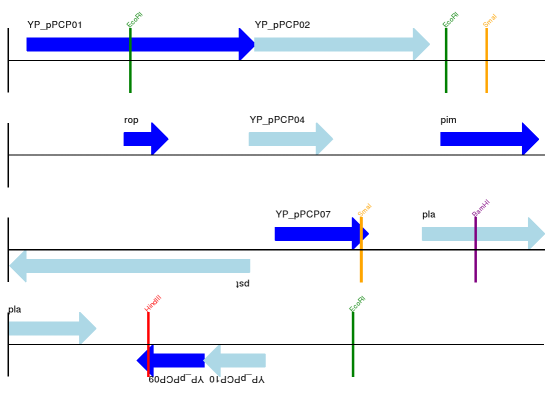
\includegraphics{plasmid_linear_nice.png}

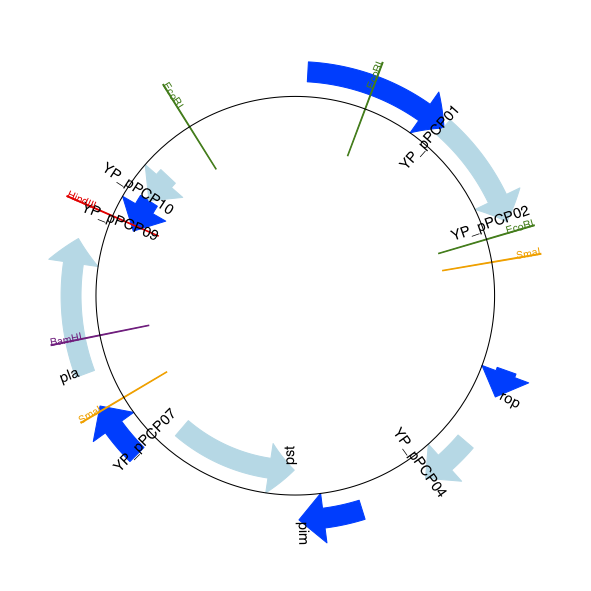
\includegraphics{plasmid_circular_nice.png}


\subsection{17.1.10 多重轨迹}
\label{chr17:id9}
前面实例中都是单独的track,我们可以创建多个track,比如,一个track展示基因,另一个track展示重复序列。Proux等人2002年报道的文章 {[}{\hyperref[chr17:proux2002]{5}}{]} 中图6是一个很好的范例,下面我们将三个噬菌体基因组依次进行展示。首先需要三个噬菌体的GenBank文件。
\begin{itemize}
\item {} 
\code{NC\_002703} – Lactococcus phage Tuc2009, 全基因组大小 (38347 bp)

\item {} 
\code{AF323668} – Bacteriophage bIL285, 全基因组大小(35538 bp)

\item {} 
\code{NC\_003212} – \emph{Listeria innocua} Clip11262,我们将仅关注前噬菌体5的全基因组 (长度大体相同).

\end{itemize}

这三个文件可以从Entrez下载,详情请查阅 {\hyperref[chr09:sec-efetch]{\emph{9.6}}} 。从三个噬菌体基因组文件中分离(slice)提取相关Features信息(请查阅 {\hyperref[chr04:sec-seqrecord-slicing]{\emph{4.6}}} ),保证前两个噬菌体的反向互补链与其起始点对齐,再次保存Feature(详情请查阅 {\hyperref[chr04:sec-seqrecord-reverse-complement]{\emph{4.8}}} )。
\DUspan{keyword,namespace}{}\DUspan{name,namespace}{}\DUspan{keyword,namespace}{}\DUspan{name}{}\DUspan{name}{}\DUspan{operator}{}\DUspan{name}{}\DUspan{operator}{}\DUspan{name}{}\DUspan{punctuation}{}\DUspan{literal,string}{}\DUspan{punctuation}{}\DUspan{literal,string}{}\DUspan{punctuation}{}\DUspan{name}{}\DUspan{operator}{}\DUspan{name}{}\DUspan{operator}{}\DUspan{name}{}\DUspan{punctuation}{}\DUspan{literal,string}{}\DUspan{punctuation}{}\DUspan{literal,string}{}\DUspan{punctuation}{}\DUspan{name}{}\DUspan{operator}{}\DUspan{name}{}\DUspan{operator}{}\DUspan{name}{}\DUspan{punctuation}{}\DUspan{literal,string}{}\DUspan{punctuation}{}\DUspan{literal,string}{}\DUspan{punctuation}{}\DUspan{literal,number,integer}{}\DUspan{punctuation}{}\DUspan{literal,number,integer}{}\DUspan{punctuation}{}\DUspan{operator}{}\DUspan{name}{}\DUspan{punctuation}{}\DUspan{name}{}\DUspan{operator}{}\DUspan{name,builtin,pseudo}{}\DUspan{punctuation}{}
\begin{Verbatim}[commandchars=\\\{\}]
\PYG{k+kn}{from} \PYG{n+nn}{Bio} \PYG{k+kn}{import} \PYG{n}{SeqIO}

\PYG{n}{A\PYGZus{}rec} \PYG{o}{=} \PYG{n}{SeqIO}\PYG{o}{.}\PYG{n}{read}\PYG{p}{(}\PYG{l+s}{\PYGZdq{}}\PYG{l+s}{NC\PYGZus{}002703.gbk}\PYG{l+s}{\PYGZdq{}}\PYG{p}{,} \PYG{l+s}{\PYGZdq{}}\PYG{l+s}{gb}\PYG{l+s}{\PYGZdq{}}\PYG{p}{)}
\PYG{n}{B\PYGZus{}rec} \PYG{o}{=} \PYG{n}{SeqIO}\PYG{o}{.}\PYG{n}{read}\PYG{p}{(}\PYG{l+s}{\PYGZdq{}}\PYG{l+s}{AF323668.gbk}\PYG{l+s}{\PYGZdq{}}\PYG{p}{,} \PYG{l+s}{\PYGZdq{}}\PYG{l+s}{gb}\PYG{l+s}{\PYGZdq{}}\PYG{p}{)}
\PYG{n}{C\PYGZus{}rec} \PYG{o}{=} \PYG{n}{SeqIO}\PYG{o}{.}\PYG{n}{read}\PYG{p}{(}\PYG{l+s}{\PYGZdq{}}\PYG{l+s}{NC\PYGZus{}003212.gbk}\PYG{l+s}{\PYGZdq{}}\PYG{p}{,} \PYG{l+s}{\PYGZdq{}}\PYG{l+s}{gb}\PYG{l+s}{\PYGZdq{}}\PYG{p}{)}\PYG{p}{[}\PYG{l+m+mi}{2587879}\PYG{p}{:}\PYG{l+m+mi}{2625807}\PYG{p}{]}\PYG{o}{.}\PYG{n}{reverse\PYGZus{}complement}\PYG{p}{(}\PYG{n}{name}\PYG{o}{=}\PYG{n+nb+bp}{True}\PYG{p}{)}
\end{Verbatim}

图像中用不同颜色表示基因功能的差异。这需要编辑GenBank文件中每一个feature的颜色参数——就像用  \href{http://www.sanger.ac.uk/resources/software/artemis/}{Sanger’s Artemis
editor} 处理 ——才能被GenomeDiagram识别。但是,这里只需要硬编码(hard code)三个颜色列表。

上述GenBank文件中的注释信息与Proux所用的文件信息并不完全相同,他们还添加了一些未注释的基因。
\DUspan{keyword,namespace}{}\DUspan{name,namespace}{}\DUspan{keyword,namespace}{}\DUspan{name}{}\DUspan{punctuation}{}\DUspan{name}{}\DUspan{punctuation}{}\DUspan{name}{}\DUspan{punctuation}{}\DUspan{name}{}\DUspan{punctuation}{}\DUspan{name}{}\DUspan{punctuation}{}\DUspan{name}{}\DUspan{punctuation}{}\DUspan{name}{}\DUspan{punctuation}{}\DUspan{name}{}\DUspan{name}{}\DUspan{operator}{}\DUspan{punctuation}{}\DUspan{name}{}\DUspan{punctuation}{}\DUspan{operator}{}\DUspan{literal,number,integer}{}\DUspan{operator}{}\DUspan{punctuation}{}\DUspan{name}{}\DUspan{punctuation}{}\DUspan{operator}{}\DUspan{literal,number,integer}{}\DUspan{operator}{}\DUspan{punctuation}{}\DUspan{name}{}\DUspan{punctuation}{}\DUspan{operator}{}\DUspan{literal,number,integer}{}\DUspan{operator}{}\DUspan{punctuation}{}\DUspan{name}{}\DUspan{punctuation}{}\DUspan{operator}{}\DUspan{literal,number,integer}{}\DUspan{operator}{}\DUspan{punctuation}{}\DUspan{name}{}\DUspan{punctuation}{}\DUspan{operator}{}\DUspan{punctuation}{}\DUspan{name}{}\DUspan{punctuation}{}\DUspan{operator}{}\DUspan{literal,number,integer}{}\DUspan{operator}{}\DUspan{punctuation}{}\DUspan{name}{}\DUspan{punctuation}{}\DUspan{operator}{}\DUspan{literal,number,integer}{}\DUspan{operator}{}\DUspan{punctuation}{}\DUspan{name}{}\DUspan{punctuation}{}\DUspan{operator}{}\DUspan{punctuation}{}\DUspan{name}{}\DUspan{punctuation}{}\DUspan{operator}{}\DUspan{literal,number,integer}{}\DUspan{operator}{}\DUspan{punctuation}{}\DUspan{name}{}\DUspan{punctuation}{}\DUspan{name}{}\DUspan{punctuation}{}\DUspan{operator}{}\DUspan{punctuation}{}\DUspan{name}{}\DUspan{punctuation}{}\DUspan{operator}{}\DUspan{literal,number,integer}{}\DUspan{operator}{}\DUspan{punctuation}{}\DUspan{name}{}\DUspan{punctuation}{}\DUspan{operator}{}\DUspan{literal,number,integer}{}\DUspan{operator}{}\DUspan{punctuation}{}\DUspan{name}{}\DUspan{punctuation}{}\DUspan{operator}{}\DUspan{literal,number,integer}{}\DUspan{operator}{}\DUspan{punctuation}{}\DUspan{name}{}\DUspan{punctuation}{}\DUspan{name}{}\DUspan{punctuation}{}\DUspan{operator}{}\DUspan{punctuation}{}\DUspan{name}{}\DUspan{punctuation}{}\DUspan{operator}{}\DUspan{literal,number,integer}{}\DUspan{operator}{}\DUspan{punctuation}{}\DUspan{name}{}\DUspan{punctuation}{}\DUspan{name}{}\DUspan{operator}{}\DUspan{punctuation}{}\DUspan{name}{}\DUspan{punctuation}{}\DUspan{operator}{}\DUspan{literal,number,integer}{}\DUspan{operator}{}\DUspan{punctuation}{}\DUspan{name}{}\DUspan{punctuation}{}\DUspan{operator}{}\DUspan{literal,number,integer}{}\DUspan{operator}{}\DUspan{punctuation}{}\DUspan{name}{}\DUspan{punctuation}{}\DUspan{operator}{}\DUspan{literal,number,integer}{}\DUspan{operator}{}\DUspan{punctuation}{}\DUspan{name}{}\DUspan{punctuation}{}\DUspan{operator}{}\DUspan{punctuation}{}\DUspan{name}{}\DUspan{punctuation}{}\DUspan{operator}{}\DUspan{punctuation}{}\DUspan{name}{}\DUspan{punctuation}{}\DUspan{operator}{}\DUspan{literal,number,integer}{}\DUspan{operator}{}\DUspan{punctuation}{}\DUspan{name}{}\DUspan{punctuation}{}\DUspan{operator}{}\DUspan{literal,number,integer}{}\DUspan{operator}{}\DUspan{punctuation}{}\DUspan{name}{}\DUspan{punctuation}{}\DUspan{operator}{}\DUspan{punctuation}{}\DUspan{name}{}\DUspan{punctuation}{}\DUspan{operator}{}\DUspan{literal,number,integer}{}\DUspan{operator}{}\DUspan{punctuation}{}\DUspan{name}{}\DUspan{punctuation}{}\DUspan{operator}{}\DUspan{literal,number,integer}{}\DUspan{operator}{}\DUspan{punctuation}{}\DUspan{name}{}\DUspan{punctuation}{}\DUspan{operator}{}\DUspan{literal,number,integer}{}\DUspan{operator}{}\DUspan{punctuation}{}\DUspan{name}{}\DUspan{punctuation}{}\DUspan{operator}{}\DUspan{literal,number,integer}{}\DUspan{operator}{}\DUspan{punctuation}{}\DUspan{name}{}\DUspan{punctuation}{}\DUspan{operator}{}\DUspan{literal,number,integer}{}\DUspan{name}{}\DUspan{operator}{}\DUspan{punctuation}{}\DUspan{name}{}\DUspan{punctuation}{}\DUspan{operator}{}\DUspan{literal,number,integer}{}\DUspan{operator}{}\DUspan{punctuation}{}\DUspan{name}{}\DUspan{punctuation}{}\DUspan{operator}{}\DUspan{literal,number,integer}{}\DUspan{operator}{}\DUspan{punctuation}{}\DUspan{name}{}\DUspan{punctuation}{}\DUspan{operator}{}\DUspan{literal,number,integer}{}\DUspan{operator}{}\DUspan{punctuation}{}\DUspan{name}{}\DUspan{punctuation}{}\DUspan{operator}{}\DUspan{literal,number,integer}{}\DUspan{operator}{}\DUspan{punctuation}{}\DUspan{name}{}\DUspan{punctuation}{}\DUspan{name}{}\DUspan{punctuation}{}\DUspan{operator}{}\DUspan{punctuation}{}\DUspan{name}{}\DUspan{punctuation}{}\DUspan{operator}{}\DUspan{literal,number,integer}{}\DUspan{operator}{}\DUspan{punctuation}{}\DUspan{name}{}\DUspan{punctuation}{}\DUspan{operator}{}\DUspan{literal,number,integer}{}
\begin{Verbatim}[commandchars=\\\{\}]
\PYG{k+kn}{from} \PYG{n+nn}{reportlab.lib.colors} \PYG{k+kn}{import} \PYG{n}{red}\PYG{p}{,} \PYG{n}{grey}\PYG{p}{,} \PYG{n}{orange}\PYG{p}{,} \PYG{n}{green}\PYG{p}{,} \PYG{n}{brown}\PYG{p}{,} \PYG{n}{blue}\PYG{p}{,} \PYG{n}{lightblue}\PYG{p}{,} \PYG{n}{purple}

\PYG{n}{A\PYGZus{}colors} \PYG{o}{=} \PYG{p}{[}\PYG{n}{red}\PYG{p}{]}\PYG{o}{*}\PYG{l+m+mi}{5} \PYG{o}{+} \PYG{p}{[}\PYG{n}{grey}\PYG{p}{]}\PYG{o}{*}\PYG{l+m+mi}{7} \PYG{o}{+} \PYG{p}{[}\PYG{n}{orange}\PYG{p}{]}\PYG{o}{*}\PYG{l+m+mi}{2} \PYG{o}{+} \PYG{p}{[}\PYG{n}{grey}\PYG{p}{]}\PYG{o}{*}\PYG{l+m+mi}{2} \PYG{o}{+} \PYG{p}{[}\PYG{n}{orange}\PYG{p}{]} \PYG{o}{+} \PYG{p}{[}\PYG{n}{grey}\PYG{p}{]}\PYG{o}{*}\PYG{l+m+mi}{11} \PYG{o}{+} \PYG{p}{[}\PYG{n}{green}\PYG{p}{]}\PYG{o}{*}\PYG{l+m+mi}{4} \PYGZbs{}
         \PYG{o}{+} \PYG{p}{[}\PYG{n}{grey}\PYG{p}{]} \PYG{o}{+} \PYG{p}{[}\PYG{n}{green}\PYG{p}{]}\PYG{o}{*}\PYG{l+m+mi}{2} \PYG{o}{+} \PYG{p}{[}\PYG{n}{grey}\PYG{p}{,} \PYG{n}{green}\PYG{p}{]} \PYG{o}{+} \PYG{p}{[}\PYG{n}{brown}\PYG{p}{]}\PYG{o}{*}\PYG{l+m+mi}{5} \PYG{o}{+} \PYG{p}{[}\PYG{n}{blue}\PYG{p}{]}\PYG{o}{*}\PYG{l+m+mi}{4} \PYG{o}{+} \PYG{p}{[}\PYG{n}{lightblue}\PYG{p}{]}\PYG{o}{*}\PYG{l+m+mi}{5} \PYGZbs{}
         \PYG{o}{+} \PYG{p}{[}\PYG{n}{grey}\PYG{p}{,} \PYG{n}{lightblue}\PYG{p}{]} \PYG{o}{+} \PYG{p}{[}\PYG{n}{purple}\PYG{p}{]}\PYG{o}{*}\PYG{l+m+mi}{2} \PYG{o}{+} \PYG{p}{[}\PYG{n}{grey}\PYG{p}{]}
\PYG{n}{B\PYGZus{}colors} \PYG{o}{=} \PYG{p}{[}\PYG{n}{red}\PYG{p}{]}\PYG{o}{*}\PYG{l+m+mi}{6} \PYG{o}{+} \PYG{p}{[}\PYG{n}{grey}\PYG{p}{]}\PYG{o}{*}\PYG{l+m+mi}{8} \PYG{o}{+} \PYG{p}{[}\PYG{n}{orange}\PYG{p}{]}\PYG{o}{*}\PYG{l+m+mi}{2} \PYG{o}{+} \PYG{p}{[}\PYG{n}{grey}\PYG{p}{]} \PYG{o}{+} \PYG{p}{[}\PYG{n}{orange}\PYG{p}{]} \PYG{o}{+} \PYG{p}{[}\PYG{n}{grey}\PYG{p}{]}\PYG{o}{*}\PYG{l+m+mi}{21} \PYG{o}{+} \PYG{p}{[}\PYG{n}{green}\PYG{p}{]}\PYG{o}{*}\PYG{l+m+mi}{5} \PYGZbs{}
         \PYG{o}{+} \PYG{p}{[}\PYG{n}{grey}\PYG{p}{]} \PYG{o}{+} \PYG{p}{[}\PYG{n}{brown}\PYG{p}{]}\PYG{o}{*}\PYG{l+m+mi}{4} \PYG{o}{+} \PYG{p}{[}\PYG{n}{blue}\PYG{p}{]}\PYG{o}{*}\PYG{l+m+mi}{3} \PYG{o}{+} \PYG{p}{[}\PYG{n}{lightblue}\PYG{p}{]}\PYG{o}{*}\PYG{l+m+mi}{3} \PYG{o}{+} \PYG{p}{[}\PYG{n}{grey}\PYG{p}{]}\PYG{o}{*}\PYG{l+m+mi}{5} \PYG{o}{+} \PYG{p}{[}\PYG{n}{purple}\PYG{p}{]}\PYG{o}{*}\PYG{l+m+mi}{2}
\PYG{n}{C\PYGZus{}colors} \PYG{o}{=} \PYG{p}{[}\PYG{n}{grey}\PYG{p}{]}\PYG{o}{*}\PYG{l+m+mi}{30} \PYG{o}{+} \PYG{p}{[}\PYG{n}{green}\PYG{p}{]}\PYG{o}{*}\PYG{l+m+mi}{5} \PYG{o}{+} \PYG{p}{[}\PYG{n}{brown}\PYG{p}{]}\PYG{o}{*}\PYG{l+m+mi}{4} \PYG{o}{+} \PYG{p}{[}\PYG{n}{blue}\PYG{p}{]}\PYG{o}{*}\PYG{l+m+mi}{2} \PYG{o}{+} \PYG{p}{[}\PYG{n}{grey}\PYG{p}{,} \PYG{n}{blue}\PYG{p}{]} \PYG{o}{+} \PYG{p}{[}\PYG{n}{lightblue}\PYG{p}{]}\PYG{o}{*}\PYG{l+m+mi}{2} \PYGZbs{}
         \PYG{o}{+} \PYG{p}{[}\PYG{n}{grey}\PYG{p}{]}\PYG{o}{*}\PYG{l+m+mi}{5}
\end{Verbatim}

接下来是“draw”方法,给diagram添加3个track。我们在示例中设置不同的开始/结束值来体现它们之间长度不等(Biopython 1.59及更高级的版本)。
\DUspan{keyword,namespace}{}\DUspan{name,namespace}{}\DUspan{keyword,namespace}{}\DUspan{name}{}\DUspan{name}{}\DUspan{operator}{}\DUspan{literal,string}{}\DUspan{name}{}\DUspan{operator}{}\DUspan{name}{}\DUspan{operator}{}\DUspan{name}{}\DUspan{punctuation}{}\DUspan{name}{}\DUspan{punctuation}{}\DUspan{name}{}\DUspan{operator}{}\DUspan{literal,number,integer}{}\DUspan{keyword}{}\DUspan{name}{}\DUspan{punctuation}{}\DUspan{name}{}\DUspan{operator,word}{}\DUspan{name,builtin}{}\DUspan{punctuation}{}\DUspan{name}{}\DUspan{punctuation}{}\DUspan{name}{}\DUspan{punctuation}{}\DUspan{name}{}\DUspan{punctuation}{}\DUspan{punctuation}{}\DUspan{name}{}\DUspan{punctuation}{}\DUspan{name}{}\DUspan{punctuation}{}\DUspan{name}{}\DUspan{punctuation}{}\DUspan{name}{}\DUspan{operator}{}\DUspan{name,builtin}{}\DUspan{punctuation}{}\DUspan{name}{}\DUspan{punctuation}{}\DUspan{name,builtin}{}\DUspan{punctuation}{}\DUspan{name}{}\DUspan{punctuation}{}\DUspan{name}{}\DUspan{operator}{}\DUspan{name}{}\DUspan{operator}{}\DUspan{name}{}\DUspan{punctuation}{}\DUspan{literal,number,integer}{}\DUspan{punctuation}{}\DUspan{name}{}\DUspan{operator}{}\DUspan{name}{}\DUspan{operator}{}\DUspan{name}{}\DUspan{punctuation}{}\DUspan{name}{}\DUspan{operator}{}\DUspan{name,builtin,pseudo}{}\DUspan{punctuation}{}\DUspan{name}{}\DUspan{operator}{}\DUspan{literal,number,integer}{}\DUspan{punctuation}{}\DUspan{name}{}\DUspan{operator}{}\DUspan{name,builtin}{}\DUspan{punctuation}{}\DUspan{name}{}\DUspan{punctuation}{}\DUspan{name}{}\DUspan{operator}{}\DUspan{name}{}\DUspan{operator}{}\DUspan{name}{}\DUspan{punctuation}{}\DUspan{name}{}\DUspan{operator}{}\DUspan{literal,number,integer}{}\DUspan{keyword}{}\DUspan{name}{}\DUspan{operator,word}{}\DUspan{name}{}\DUspan{operator}{}\DUspan{name}{}\DUspan{punctuation}{}\DUspan{keyword}{}\DUspan{name}{}\DUspan{operator}{}\DUspan{name}{}\DUspan{operator}{}\DUspan{literal,string}{}\DUspan{punctuation}{}\DUspan{comment}{}\DUspan{keyword}{}\DUspan{name}{}\DUspan{operator}{}\DUspan{name}{}\DUspan{punctuation}{}\DUspan{name}{}\DUspan{punctuation}{}\DUspan{name}{}\DUspan{operator}{}\DUspan{literal,string}{}\DUspan{punctuation}{}\DUspan{name}{}\DUspan{operator}{}\DUspan{name}{}\DUspan{punctuation}{}\DUspan{name}{}\DUspan{punctuation}{}\DUspan{name}{}\DUspan{operator}{}\DUspan{name,builtin,pseudo}{}\DUspan{punctuation}{}\DUspan{name}{}\DUspan{operator}{}\DUspan{name,builtin}{}\DUspan{punctuation}{}\DUspan{name}{}\DUspan{operator}{}\DUspan{literal,number,integer}{}\DUspan{punctuation}{}\DUspan{name}{}\DUspan{operator}{}\DUspan{literal,string}{}\DUspan{punctuation}{}\DUspan{name}{}\DUspan{operator}{}\DUspan{literal,number,integer}{}\DUspan{punctuation}{}\DUspan{name}{}\DUspan{operator}{}\DUspan{literal,number,integer}{}\DUspan{punctuation}{}\DUspan{name}{}\DUspan{operator}{}\DUspan{literal,number,integer}{}\DUspan{name}{}\DUspan{operator}{}\DUspan{name}{}\DUspan{punctuation}{}\DUspan{name}{}\DUspan{operator}{}\DUspan{literal,string}{}\DUspan{punctuation}{}\DUspan{name}{}\DUspan{operator}{}\DUspan{literal,string}{}\DUspan{punctuation}{}\DUspan{name}{}\DUspan{operator}{}\DUspan{literal,number,integer}{}\DUspan{punctuation}{}\DUspan{name}{}\DUspan{operator}{}\DUspan{literal,number,integer}{}\DUspan{punctuation}{}\DUspan{name}{}\DUspan{operator}{}\DUspan{name}{}\DUspan{punctuation}{}\DUspan{name}{}\DUspan{operator}{}\DUspan{name}{}\DUspan{punctuation}{}\DUspan{name}{}\DUspan{operator}{}\DUspan{literal,string}{}\DUspan{punctuation}{}\DUspan{literal,string}{}\DUspan{punctuation}{}\DUspan{name}{}\DUspan{operator}{}\DUspan{name}{}\DUspan{punctuation}{}\DUspan{name}{}\DUspan{operator}{}\DUspan{literal,string}{}\DUspan{punctuation}{}\DUspan{literal,string}{}\DUspan{punctuation}{}\DUspan{name}{}\DUspan{operator}{}\DUspan{name}{}\DUspan{punctuation}{}\DUspan{name}{}\DUspan{operator}{}\DUspan{literal,string}{}\DUspan{punctuation}{}\DUspan{literal,string}{}\DUspan{punctuation}{}
\begin{Verbatim}[commandchars=\\\{\}]
\PYG{k+kn}{from} \PYG{n+nn}{Bio.Graphics} \PYG{k+kn}{import} \PYG{n}{GenomeDiagram}

\PYG{n}{name} \PYG{o}{=} \PYG{l+s}{\PYGZdq{}}\PYG{l+s}{Proux Fig 6}\PYG{l+s}{\PYGZdq{}}
\PYG{n}{gd\PYGZus{}diagram} \PYG{o}{=} \PYG{n}{GenomeDiagram}\PYG{o}{.}\PYG{n}{Diagram}\PYG{p}{(}\PYG{n}{name}\PYG{p}{)}
\PYG{n}{max\PYGZus{}len} \PYG{o}{=} \PYG{l+m+mi}{0}
\PYG{k}{for} \PYG{n}{record}\PYG{p}{,} \PYG{n}{gene\PYGZus{}colors} \PYG{o+ow}{in} \PYG{n+nb}{zip}\PYG{p}{(}\PYG{p}{[}\PYG{n}{A\PYGZus{}rec}\PYG{p}{,} \PYG{n}{B\PYGZus{}rec}\PYG{p}{,} \PYG{n}{C\PYGZus{}rec}\PYG{p}{]}\PYG{p}{,} \PYG{p}{[}\PYG{n}{A\PYGZus{}colors}\PYG{p}{,} \PYG{n}{B\PYGZus{}colors}\PYG{p}{,} \PYG{n}{C\PYGZus{}colors}\PYG{p}{]}\PYG{p}{)}\PYG{p}{:}
    \PYG{n}{max\PYGZus{}len} \PYG{o}{=} \PYG{n+nb}{max}\PYG{p}{(}\PYG{n}{max\PYGZus{}len}\PYG{p}{,} \PYG{n+nb}{len}\PYG{p}{(}\PYG{n}{record}\PYG{p}{)}\PYG{p}{)}
    \PYG{n}{gd\PYGZus{}track\PYGZus{}for\PYGZus{}features} \PYG{o}{=} \PYG{n}{gd\PYGZus{}diagram}\PYG{o}{.}\PYG{n}{new\PYGZus{}track}\PYG{p}{(}\PYG{l+m+mi}{1}\PYG{p}{,}
                            \PYG{n}{name}\PYG{o}{=}\PYG{n}{record}\PYG{o}{.}\PYG{n}{name}\PYG{p}{,}
                            \PYG{n}{greytrack}\PYG{o}{=}\PYG{n+nb+bp}{True}\PYG{p}{,}
                            \PYG{n}{start}\PYG{o}{=}\PYG{l+m+mi}{0}\PYG{p}{,} \PYG{n}{end}\PYG{o}{=}\PYG{n+nb}{len}\PYG{p}{(}\PYG{n}{record}\PYG{p}{)}\PYG{p}{)}
    \PYG{n}{gd\PYGZus{}feature\PYGZus{}set} \PYG{o}{=} \PYG{n}{gd\PYGZus{}track\PYGZus{}for\PYGZus{}features}\PYG{o}{.}\PYG{n}{new\PYGZus{}set}\PYG{p}{(}\PYG{p}{)}

    \PYG{n}{i} \PYG{o}{=} \PYG{l+m+mi}{0}
    \PYG{k}{for} \PYG{n}{feature} \PYG{o+ow}{in} \PYG{n}{record}\PYG{o}{.}\PYG{n}{features}\PYG{p}{:}
        \PYG{k}{if} \PYG{n}{feature}\PYG{o}{.}\PYG{n}{type} \PYG{o}{!=} \PYG{l+s}{\PYGZdq{}}\PYG{l+s}{gene}\PYG{l+s}{\PYGZdq{}}\PYG{p}{:}
            \PYG{c}{\PYGZsh{}Exclude this feature}
            \PYG{k}{continue}
        \PYG{n}{gd\PYGZus{}feature\PYGZus{}set}\PYG{o}{.}\PYG{n}{add\PYGZus{}feature}\PYG{p}{(}\PYG{n}{feature}\PYG{p}{,} \PYG{n}{sigil}\PYG{o}{=}\PYG{l+s}{\PYGZdq{}}\PYG{l+s}{ARROW}\PYG{l+s}{\PYGZdq{}}\PYG{p}{,}
                                   \PYG{n}{color}\PYG{o}{=}\PYG{n}{gene\PYGZus{}colors}\PYG{p}{[}\PYG{n}{i}\PYG{p}{]}\PYG{p}{,} \PYG{n}{label}\PYG{o}{=}\PYG{n+nb+bp}{True}\PYG{p}{,}
                                   \PYG{n}{name} \PYG{o}{=} \PYG{n+nb}{str}\PYG{p}{(}\PYG{n}{i}\PYG{o}{+}\PYG{l+m+mi}{1}\PYG{p}{)}\PYG{p}{,}
                                   \PYG{n}{label\PYGZus{}position}\PYG{o}{=}\PYG{l+s}{\PYGZdq{}}\PYG{l+s}{start}\PYG{l+s}{\PYGZdq{}}\PYG{p}{,}
                                   \PYG{n}{label\PYGZus{}size} \PYG{o}{=} \PYG{l+m+mi}{6}\PYG{p}{,} \PYG{n}{label\PYGZus{}angle}\PYG{o}{=}\PYG{l+m+mi}{0}\PYG{p}{)}
        \PYG{n}{i}\PYG{o}{+}\PYG{o}{=}\PYG{l+m+mi}{1}

\PYG{n}{gd\PYGZus{}diagram}\PYG{o}{.}\PYG{n}{draw}\PYG{p}{(}\PYG{n}{format}\PYG{o}{=}\PYG{l+s}{\PYGZdq{}}\PYG{l+s}{linear}\PYG{l+s}{\PYGZdq{}}\PYG{p}{,} \PYG{n}{pagesize}\PYG{o}{=}\PYG{l+s}{\PYGZsq{}}\PYG{l+s}{A4}\PYG{l+s}{\PYGZsq{}}\PYG{p}{,} \PYG{n}{fragments}\PYG{o}{=}\PYG{l+m+mi}{1}\PYG{p}{,}
                \PYG{n}{start}\PYG{o}{=}\PYG{l+m+mi}{0}\PYG{p}{,} \PYG{n}{end}\PYG{o}{=}\PYG{n}{max\PYGZus{}len}\PYG{p}{)}
\PYG{n}{gd\PYGZus{}diagram}\PYG{o}{.}\PYG{n}{write}\PYG{p}{(}\PYG{n}{name} \PYG{o}{+} \PYG{l+s}{\PYGZdq{}}\PYG{l+s}{.pdf}\PYG{l+s}{\PYGZdq{}}\PYG{p}{,} \PYG{l+s}{\PYGZdq{}}\PYG{l+s}{PDF}\PYG{l+s}{\PYGZdq{}}\PYG{p}{)}
\PYG{n}{gd\PYGZus{}diagram}\PYG{o}{.}\PYG{n}{write}\PYG{p}{(}\PYG{n}{name} \PYG{o}{+} \PYG{l+s}{\PYGZdq{}}\PYG{l+s}{.eps}\PYG{l+s}{\PYGZdq{}}\PYG{p}{,} \PYG{l+s}{\PYGZdq{}}\PYG{l+s}{EPS}\PYG{l+s}{\PYGZdq{}}\PYG{p}{)}
\PYG{n}{gd\PYGZus{}diagram}\PYG{o}{.}\PYG{n}{write}\PYG{p}{(}\PYG{n}{name} \PYG{o}{+} \PYG{l+s}{\PYGZdq{}}\PYG{l+s}{.svg}\PYG{l+s}{\PYGZdq{}}\PYG{p}{,} \PYG{l+s}{\PYGZdq{}}\PYG{l+s}{SVG}\PYG{l+s}{\PYGZdq{}}\PYG{p}{)}
\end{Verbatim}

结果如图所示:

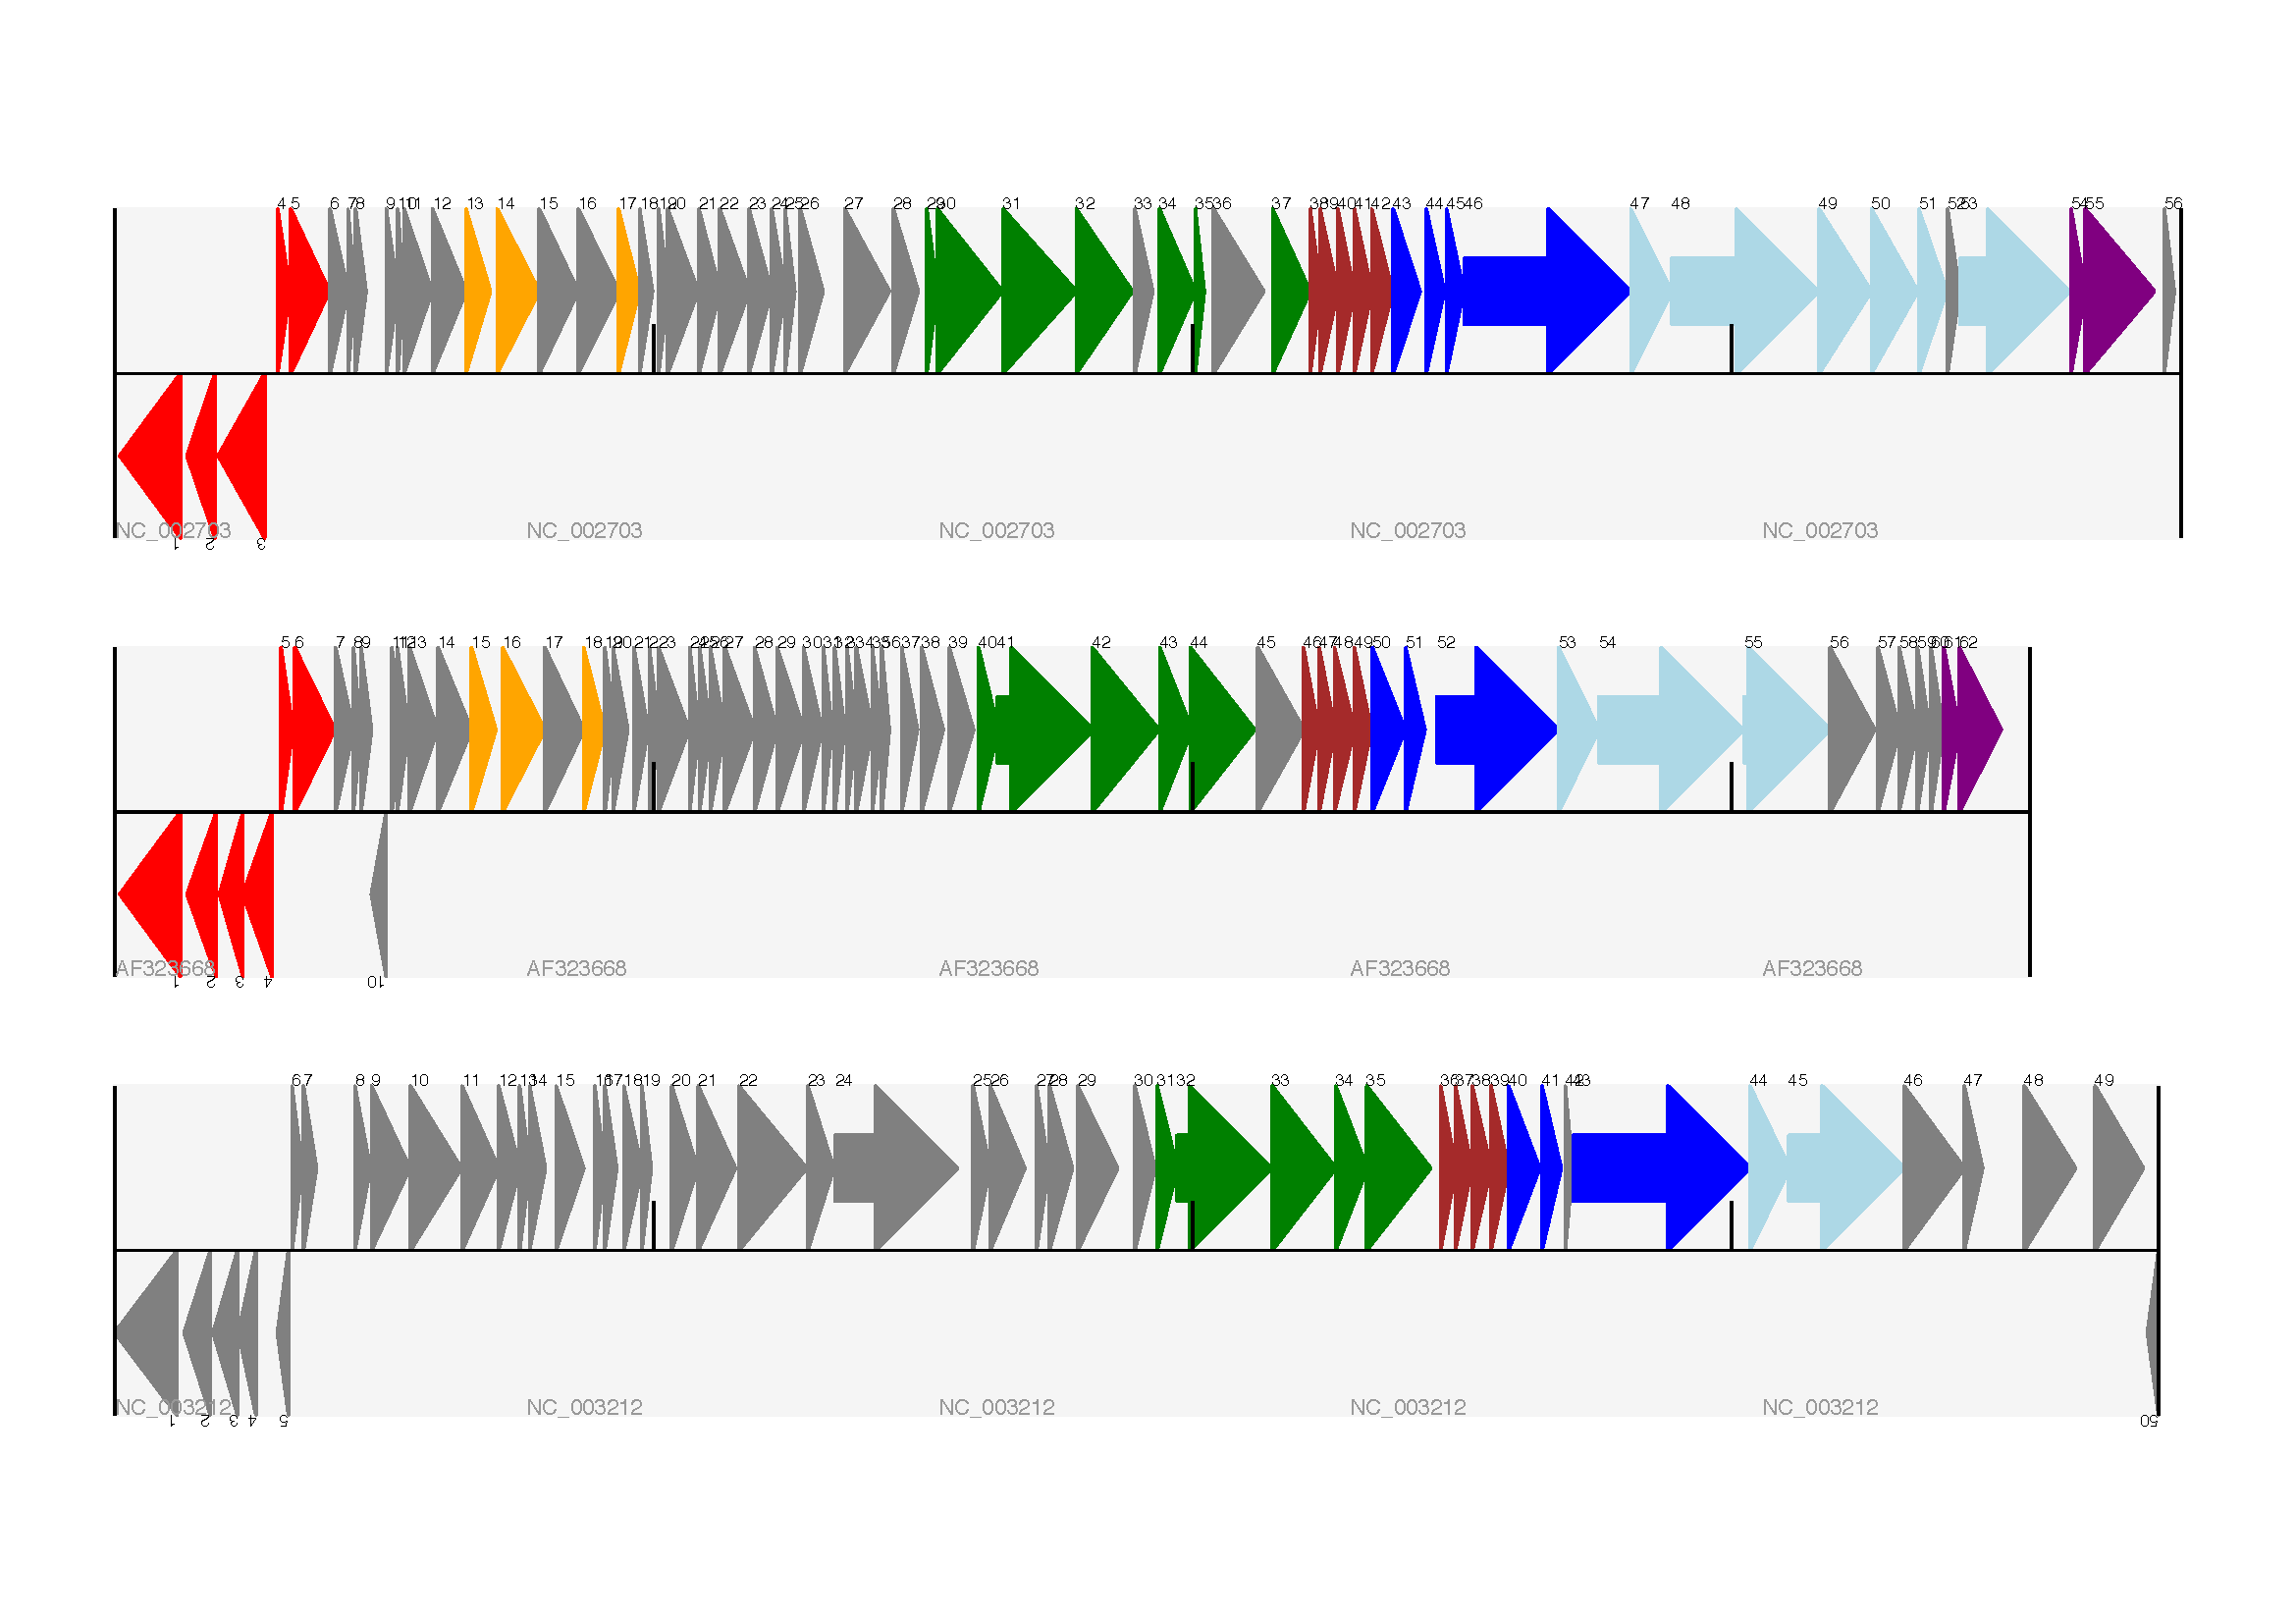
\includegraphics{three_track_simple.png}

在示例图中底部的噬菌体没有红色或橙色的基因标记。另外,三个噬菌体可视化图的长度不同,这是因为它们的比例相同,长度却不同。

另外有一点不同,不同噬菌体的同源蛋白质之间用有颜色的links相连,下一部分将解决这个问题。


\subsection{17.1.11 不同Track之间的Cross-Links}
\label{chr17:trackcross-links}
Biopython 1.59新增绘制不同track之间Cross-Links的功能,这个功能可用于将要展示的简单线形图中,也可用于将线形图分割为短片段(fragments)和环形图。

我们接着模仿Proux等人 {[}{\hyperref[chr23:proux2002]{\emph{5}}}{]} 的图像,我们需要一个包含基因之间的“cross links”、“得分”或“颜色”的列表。 实际应用中,可以从BLAST文件自动提取这些信息,这里是手动输入的。

噬菌体的名称同样表示为A,B和C。这里将要展示的是A与B之间的links,噬菌体A和B基因的相似百分比存储在元组中。
\DUspan{comment}{}\DUspan{name}{}\DUspan{operator}{}\DUspan{punctuation}{}\DUspan{punctuation}{}\DUspan{literal,number,integer}{}\DUspan{punctuation}{}\DUspan{literal,string}{}\DUspan{punctuation}{}\DUspan{literal,string}{}\DUspan{punctuation}{}\DUspan{punctuation}{}\DUspan{literal,number,integer}{}\DUspan{punctuation}{}\DUspan{literal,string}{}\DUspan{punctuation}{}\DUspan{literal,string}{}\DUspan{punctuation}{}\DUspan{punctuation}{}\DUspan{literal,number,integer}{}\DUspan{punctuation}{}\DUspan{literal,string}{}\DUspan{punctuation}{}\DUspan{literal,string}{}\DUspan{punctuation}{}\DUspan{punctuation}{}\DUspan{literal,number,integer}{}\DUspan{punctuation}{}\DUspan{literal,string}{}\DUspan{punctuation}{}\DUspan{literal,string}{}\DUspan{punctuation}{}\DUspan{punctuation}{}\DUspan{literal,number,integer}{}\DUspan{punctuation}{}\DUspan{literal,string}{}\DUspan{punctuation}{}\DUspan{literal,string}{}\DUspan{punctuation}{}\DUspan{punctuation}{}\DUspan{literal,number,integer}{}\DUspan{punctuation}{}\DUspan{literal,string}{}\DUspan{punctuation}{}\DUspan{literal,string}{}\DUspan{punctuation}{}\DUspan{punctuation}{}\DUspan{literal,number,integer}{}\DUspan{punctuation}{}\DUspan{literal,string}{}\DUspan{punctuation}{}\DUspan{literal,string}{}\DUspan{punctuation}{}\DUspan{punctuation}{}\DUspan{literal,number,integer}{}\DUspan{punctuation}{}\DUspan{literal,string}{}\DUspan{punctuation}{}\DUspan{literal,string}{}\DUspan{punctuation}{}\DUspan{punctuation}{}\DUspan{literal,number,integer}{}\DUspan{punctuation}{}\DUspan{literal,string}{}\DUspan{punctuation}{}\DUspan{literal,string}{}\DUspan{punctuation}{}\DUspan{punctuation}{}\DUspan{literal,number,integer}{}\DUspan{punctuation}{}\DUspan{literal,string}{}\DUspan{punctuation}{}\DUspan{literal,string}{}\DUspan{punctuation}{}\DUspan{punctuation}{}\DUspan{literal,number,integer}{}\DUspan{punctuation}{}\DUspan{literal,string}{}\DUspan{punctuation}{}\DUspan{literal,string}{}\DUspan{punctuation}{}\DUspan{punctuation}{}\DUspan{literal,number,integer}{}\DUspan{punctuation}{}\DUspan{literal,string}{}\DUspan{punctuation}{}\DUspan{literal,string}{}\DUspan{punctuation}{}\DUspan{punctuation}{}\DUspan{literal,number,integer}{}\DUspan{punctuation}{}\DUspan{literal,string}{}\DUspan{punctuation}{}\DUspan{literal,string}{}\DUspan{punctuation}{}\DUspan{punctuation}{}\DUspan{literal,number,integer}{}\DUspan{punctuation}{}\DUspan{literal,string}{}\DUspan{punctuation}{}\DUspan{literal,string}{}\DUspan{punctuation}{}\DUspan{punctuation}{}\DUspan{literal,number,integer}{}\DUspan{punctuation}{}\DUspan{literal,string}{}\DUspan{punctuation}{}\DUspan{literal,string}{}\DUspan{punctuation}{}\DUspan{punctuation}{}\DUspan{literal,number,integer}{}\DUspan{punctuation}{}\DUspan{literal,string}{}\DUspan{punctuation}{}\DUspan{literal,string}{}\DUspan{punctuation}{}\DUspan{punctuation}{}\DUspan{literal,number,integer}{}\DUspan{punctuation}{}\DUspan{literal,string}{}\DUspan{punctuation}{}\DUspan{literal,string}{}\DUspan{punctuation}{}\DUspan{punctuation}{}\DUspan{literal,number,integer}{}\DUspan{punctuation}{}\DUspan{literal,string}{}\DUspan{punctuation}{}\DUspan{literal,string}{}\DUspan{punctuation}{}\DUspan{punctuation}{}\DUspan{literal,number,integer}{}\DUspan{punctuation}{}\DUspan{literal,string}{}\DUspan{punctuation}{}\DUspan{literal,string}{}\DUspan{punctuation}{}\DUspan{punctuation}{}\DUspan{literal,number,integer}{}\DUspan{punctuation}{}\DUspan{literal,string}{}\DUspan{punctuation}{}\DUspan{literal,string}{}\DUspan{punctuation}{}\DUspan{punctuation}{}\DUspan{literal,number,integer}{}\DUspan{punctuation}{}\DUspan{literal,string}{}\DUspan{punctuation}{}\DUspan{literal,string}{}\DUspan{punctuation}{}\DUspan{punctuation}{}\DUspan{literal,number,integer}{}\DUspan{punctuation}{}\DUspan{literal,string}{}\DUspan{punctuation}{}\DUspan{literal,string}{}\DUspan{punctuation}{}\DUspan{punctuation}{}\DUspan{literal,number,integer}{}\DUspan{punctuation}{}\DUspan{literal,string}{}\DUspan{punctuation}{}\DUspan{literal,string}{}\DUspan{punctuation}{}\DUspan{punctuation}{}\DUspan{literal,number,integer}{}\DUspan{punctuation}{}\DUspan{literal,string}{}\DUspan{punctuation}{}\DUspan{literal,string}{}\DUspan{punctuation}{}\DUspan{punctuation}{}\DUspan{literal,number,integer}{}\DUspan{punctuation}{}\DUspan{literal,string}{}\DUspan{punctuation}{}\DUspan{literal,string}{}\DUspan{punctuation}{}\DUspan{punctuation}{}
\begin{Verbatim}[commandchars=\\\{\}]
\PYG{c}{\PYGZsh{}Tuc2009 (NC\PYGZus{}002703) vs bIL285 (AF323668)}
\PYG{n}{A\PYGZus{}vs\PYGZus{}B} \PYG{o}{=} \PYG{p}{[}
    \PYG{p}{(}\PYG{l+m+mi}{99}\PYG{p}{,} \PYG{l+s}{\PYGZdq{}}\PYG{l+s}{Tuc2009\PYGZus{}01}\PYG{l+s}{\PYGZdq{}}\PYG{p}{,} \PYG{l+s}{\PYGZdq{}}\PYG{l+s}{int}\PYG{l+s}{\PYGZdq{}}\PYG{p}{)}\PYG{p}{,}
    \PYG{p}{(}\PYG{l+m+mi}{33}\PYG{p}{,} \PYG{l+s}{\PYGZdq{}}\PYG{l+s}{Tuc2009\PYGZus{}03}\PYG{l+s}{\PYGZdq{}}\PYG{p}{,} \PYG{l+s}{\PYGZdq{}}\PYG{l+s}{orf4}\PYG{l+s}{\PYGZdq{}}\PYG{p}{)}\PYG{p}{,}
    \PYG{p}{(}\PYG{l+m+mi}{94}\PYG{p}{,} \PYG{l+s}{\PYGZdq{}}\PYG{l+s}{Tuc2009\PYGZus{}05}\PYG{l+s}{\PYGZdq{}}\PYG{p}{,} \PYG{l+s}{\PYGZdq{}}\PYG{l+s}{orf6}\PYG{l+s}{\PYGZdq{}}\PYG{p}{)}\PYG{p}{,}
    \PYG{p}{(}\PYG{l+m+mi}{100}\PYG{p}{,}\PYG{l+s}{\PYGZdq{}}\PYG{l+s}{Tuc2009\PYGZus{}06}\PYG{l+s}{\PYGZdq{}}\PYG{p}{,} \PYG{l+s}{\PYGZdq{}}\PYG{l+s}{orf7}\PYG{l+s}{\PYGZdq{}}\PYG{p}{)}\PYG{p}{,}
    \PYG{p}{(}\PYG{l+m+mi}{97}\PYG{p}{,} \PYG{l+s}{\PYGZdq{}}\PYG{l+s}{Tuc2009\PYGZus{}07}\PYG{l+s}{\PYGZdq{}}\PYG{p}{,} \PYG{l+s}{\PYGZdq{}}\PYG{l+s}{orf8}\PYG{l+s}{\PYGZdq{}}\PYG{p}{)}\PYG{p}{,}
    \PYG{p}{(}\PYG{l+m+mi}{98}\PYG{p}{,} \PYG{l+s}{\PYGZdq{}}\PYG{l+s}{Tuc2009\PYGZus{}08}\PYG{l+s}{\PYGZdq{}}\PYG{p}{,} \PYG{l+s}{\PYGZdq{}}\PYG{l+s}{orf9}\PYG{l+s}{\PYGZdq{}}\PYG{p}{)}\PYG{p}{,}
    \PYG{p}{(}\PYG{l+m+mi}{98}\PYG{p}{,} \PYG{l+s}{\PYGZdq{}}\PYG{l+s}{Tuc2009\PYGZus{}09}\PYG{l+s}{\PYGZdq{}}\PYG{p}{,} \PYG{l+s}{\PYGZdq{}}\PYG{l+s}{orf10}\PYG{l+s}{\PYGZdq{}}\PYG{p}{)}\PYG{p}{,}
    \PYG{p}{(}\PYG{l+m+mi}{100}\PYG{p}{,}\PYG{l+s}{\PYGZdq{}}\PYG{l+s}{Tuc2009\PYGZus{}10}\PYG{l+s}{\PYGZdq{}}\PYG{p}{,} \PYG{l+s}{\PYGZdq{}}\PYG{l+s}{orf12}\PYG{l+s}{\PYGZdq{}}\PYG{p}{)}\PYG{p}{,}
    \PYG{p}{(}\PYG{l+m+mi}{100}\PYG{p}{,}\PYG{l+s}{\PYGZdq{}}\PYG{l+s}{Tuc2009\PYGZus{}11}\PYG{l+s}{\PYGZdq{}}\PYG{p}{,} \PYG{l+s}{\PYGZdq{}}\PYG{l+s}{orf13}\PYG{l+s}{\PYGZdq{}}\PYG{p}{)}\PYG{p}{,}
    \PYG{p}{(}\PYG{l+m+mi}{94}\PYG{p}{,} \PYG{l+s}{\PYGZdq{}}\PYG{l+s}{Tuc2009\PYGZus{}12}\PYG{l+s}{\PYGZdq{}}\PYG{p}{,} \PYG{l+s}{\PYGZdq{}}\PYG{l+s}{orf14}\PYG{l+s}{\PYGZdq{}}\PYG{p}{)}\PYG{p}{,}
    \PYG{p}{(}\PYG{l+m+mi}{87}\PYG{p}{,} \PYG{l+s}{\PYGZdq{}}\PYG{l+s}{Tuc2009\PYGZus{}13}\PYG{l+s}{\PYGZdq{}}\PYG{p}{,} \PYG{l+s}{\PYGZdq{}}\PYG{l+s}{orf15}\PYG{l+s}{\PYGZdq{}}\PYG{p}{)}\PYG{p}{,}
    \PYG{p}{(}\PYG{l+m+mi}{94}\PYG{p}{,} \PYG{l+s}{\PYGZdq{}}\PYG{l+s}{Tuc2009\PYGZus{}14}\PYG{l+s}{\PYGZdq{}}\PYG{p}{,} \PYG{l+s}{\PYGZdq{}}\PYG{l+s}{orf16}\PYG{l+s}{\PYGZdq{}}\PYG{p}{)}\PYG{p}{,}
    \PYG{p}{(}\PYG{l+m+mi}{94}\PYG{p}{,} \PYG{l+s}{\PYGZdq{}}\PYG{l+s}{Tuc2009\PYGZus{}15}\PYG{l+s}{\PYGZdq{}}\PYG{p}{,} \PYG{l+s}{\PYGZdq{}}\PYG{l+s}{orf17}\PYG{l+s}{\PYGZdq{}}\PYG{p}{)}\PYG{p}{,}
    \PYG{p}{(}\PYG{l+m+mi}{88}\PYG{p}{,} \PYG{l+s}{\PYGZdq{}}\PYG{l+s}{Tuc2009\PYGZus{}17}\PYG{l+s}{\PYGZdq{}}\PYG{p}{,} \PYG{l+s}{\PYGZdq{}}\PYG{l+s}{rusA}\PYG{l+s}{\PYGZdq{}}\PYG{p}{)}\PYG{p}{,}
    \PYG{p}{(}\PYG{l+m+mi}{91}\PYG{p}{,} \PYG{l+s}{\PYGZdq{}}\PYG{l+s}{Tuc2009\PYGZus{}18}\PYG{l+s}{\PYGZdq{}}\PYG{p}{,} \PYG{l+s}{\PYGZdq{}}\PYG{l+s}{orf20}\PYG{l+s}{\PYGZdq{}}\PYG{p}{)}\PYG{p}{,}
    \PYG{p}{(}\PYG{l+m+mi}{93}\PYG{p}{,} \PYG{l+s}{\PYGZdq{}}\PYG{l+s}{Tuc2009\PYGZus{}19}\PYG{l+s}{\PYGZdq{}}\PYG{p}{,} \PYG{l+s}{\PYGZdq{}}\PYG{l+s}{orf22}\PYG{l+s}{\PYGZdq{}}\PYG{p}{)}\PYG{p}{,}
    \PYG{p}{(}\PYG{l+m+mi}{71}\PYG{p}{,} \PYG{l+s}{\PYGZdq{}}\PYG{l+s}{Tuc2009\PYGZus{}20}\PYG{l+s}{\PYGZdq{}}\PYG{p}{,} \PYG{l+s}{\PYGZdq{}}\PYG{l+s}{orf23}\PYG{l+s}{\PYGZdq{}}\PYG{p}{)}\PYG{p}{,}
    \PYG{p}{(}\PYG{l+m+mi}{51}\PYG{p}{,} \PYG{l+s}{\PYGZdq{}}\PYG{l+s}{Tuc2009\PYGZus{}22}\PYG{l+s}{\PYGZdq{}}\PYG{p}{,} \PYG{l+s}{\PYGZdq{}}\PYG{l+s}{orf27}\PYG{l+s}{\PYGZdq{}}\PYG{p}{)}\PYG{p}{,}
    \PYG{p}{(}\PYG{l+m+mi}{97}\PYG{p}{,} \PYG{l+s}{\PYGZdq{}}\PYG{l+s}{Tuc2009\PYGZus{}23}\PYG{l+s}{\PYGZdq{}}\PYG{p}{,} \PYG{l+s}{\PYGZdq{}}\PYG{l+s}{orf28}\PYG{l+s}{\PYGZdq{}}\PYG{p}{)}\PYG{p}{,}
    \PYG{p}{(}\PYG{l+m+mi}{88}\PYG{p}{,} \PYG{l+s}{\PYGZdq{}}\PYG{l+s}{Tuc2009\PYGZus{}24}\PYG{l+s}{\PYGZdq{}}\PYG{p}{,} \PYG{l+s}{\PYGZdq{}}\PYG{l+s}{orf29}\PYG{l+s}{\PYGZdq{}}\PYG{p}{)}\PYG{p}{,}
    \PYG{p}{(}\PYG{l+m+mi}{26}\PYG{p}{,} \PYG{l+s}{\PYGZdq{}}\PYG{l+s}{Tuc2009\PYGZus{}26}\PYG{l+s}{\PYGZdq{}}\PYG{p}{,} \PYG{l+s}{\PYGZdq{}}\PYG{l+s}{orf38}\PYG{l+s}{\PYGZdq{}}\PYG{p}{)}\PYG{p}{,}
    \PYG{p}{(}\PYG{l+m+mi}{19}\PYG{p}{,} \PYG{l+s}{\PYGZdq{}}\PYG{l+s}{Tuc2009\PYGZus{}46}\PYG{l+s}{\PYGZdq{}}\PYG{p}{,} \PYG{l+s}{\PYGZdq{}}\PYG{l+s}{orf52}\PYG{l+s}{\PYGZdq{}}\PYG{p}{)}\PYG{p}{,}
    \PYG{p}{(}\PYG{l+m+mi}{77}\PYG{p}{,} \PYG{l+s}{\PYGZdq{}}\PYG{l+s}{Tuc2009\PYGZus{}48}\PYG{l+s}{\PYGZdq{}}\PYG{p}{,} \PYG{l+s}{\PYGZdq{}}\PYG{l+s}{orf54}\PYG{l+s}{\PYGZdq{}}\PYG{p}{)}\PYG{p}{,}
    \PYG{p}{(}\PYG{l+m+mi}{91}\PYG{p}{,} \PYG{l+s}{\PYGZdq{}}\PYG{l+s}{Tuc2009\PYGZus{}49}\PYG{l+s}{\PYGZdq{}}\PYG{p}{,} \PYG{l+s}{\PYGZdq{}}\PYG{l+s}{orf55}\PYG{l+s}{\PYGZdq{}}\PYG{p}{)}\PYG{p}{,}
    \PYG{p}{(}\PYG{l+m+mi}{95}\PYG{p}{,} \PYG{l+s}{\PYGZdq{}}\PYG{l+s}{Tuc2009\PYGZus{}52}\PYG{l+s}{\PYGZdq{}}\PYG{p}{,} \PYG{l+s}{\PYGZdq{}}\PYG{l+s}{orf60}\PYG{l+s}{\PYGZdq{}}\PYG{p}{)}\PYG{p}{,}
\PYG{p}{]}
\end{Verbatim}

对噬菌体B和C做同样的处理:
\DUspan{comment}{}\DUspan{name}{}\DUspan{operator}{}\DUspan{punctuation}{}\DUspan{punctuation}{}\DUspan{literal,number,integer}{}\DUspan{punctuation}{}\DUspan{literal,string}{}\DUspan{punctuation}{}\DUspan{literal,string}{}\DUspan{punctuation}{}\DUspan{punctuation}{}\DUspan{literal,number,integer}{}\DUspan{punctuation}{}\DUspan{literal,string}{}\DUspan{punctuation}{}\DUspan{literal,string}{}\DUspan{punctuation}{}\DUspan{punctuation}{}\DUspan{literal,number,integer}{}\DUspan{punctuation}{}\DUspan{literal,string}{}\DUspan{punctuation}{}\DUspan{literal,string}{}\DUspan{punctuation}{}\DUspan{comment}{}\DUspan{punctuation}{}\DUspan{literal,number,integer}{}\DUspan{punctuation}{}\DUspan{literal,string}{}\DUspan{punctuation}{}\DUspan{literal,string}{}\DUspan{punctuation}{}\DUspan{comment}{}\DUspan{punctuation}{}\DUspan{literal,number,integer}{}\DUspan{punctuation}{}\DUspan{literal,string}{}\DUspan{punctuation}{}\DUspan{literal,string}{}\DUspan{punctuation}{}\DUspan{comment}{}\DUspan{punctuation}{}\DUspan{literal,number,integer}{}\DUspan{punctuation}{}\DUspan{literal,string}{}\DUspan{punctuation}{}\DUspan{literal,string}{}\DUspan{punctuation}{}\DUspan{comment}{}\DUspan{punctuation}{}\DUspan{literal,number,integer}{}\DUspan{punctuation}{}\DUspan{literal,string}{}\DUspan{punctuation}{}\DUspan{literal,string}{}\DUspan{punctuation}{}\DUspan{punctuation}{}\DUspan{literal,number,integer}{}\DUspan{punctuation}{}\DUspan{literal,string}{}\DUspan{punctuation}{}\DUspan{literal,string}{}\DUspan{punctuation}{}\DUspan{punctuation}{}\DUspan{literal,number,integer}{}\DUspan{punctuation}{}\DUspan{literal,string}{}\DUspan{punctuation}{}\DUspan{literal,string}{}\DUspan{punctuation}{}\DUspan{punctuation}{}\DUspan{literal,number,integer}{}\DUspan{punctuation}{}\DUspan{literal,string}{}\DUspan{punctuation}{}\DUspan{literal,string}{}\DUspan{punctuation}{}\DUspan{punctuation}{}\DUspan{literal,number,integer}{}\DUspan{punctuation}{}\DUspan{literal,string}{}\DUspan{punctuation}{}\DUspan{literal,string}{}\DUspan{punctuation}{}\DUspan{punctuation}{}\DUspan{literal,number,integer}{}\DUspan{punctuation}{}\DUspan{literal,string}{}\DUspan{punctuation}{}\DUspan{literal,string}{}\DUspan{punctuation}{}\DUspan{punctuation}{}\DUspan{literal,number,integer}{}\DUspan{punctuation}{}\DUspan{literal,string}{}\DUspan{punctuation}{}\DUspan{literal,string}{}\DUspan{punctuation}{}\DUspan{punctuation}{}\DUspan{literal,number,integer}{}\DUspan{punctuation}{}\DUspan{literal,string}{}\DUspan{punctuation}{}\DUspan{literal,string}{}\DUspan{punctuation}{}\DUspan{punctuation}{}\DUspan{literal,number,integer}{}\DUspan{punctuation}{}\DUspan{literal,string}{}\DUspan{punctuation}{}\DUspan{literal,string}{}\DUspan{punctuation}{}\DUspan{punctuation}{}
\begin{Verbatim}[commandchars=\\\{\}]
\PYG{c}{\PYGZsh{}bIL285 (AF323668) vs Listeria innocua prophage 5 (in NC\PYGZus{}003212)}
\PYG{n}{B\PYGZus{}vs\PYGZus{}C} \PYG{o}{=} \PYG{p}{[}
    \PYG{p}{(}\PYG{l+m+mi}{42}\PYG{p}{,} \PYG{l+s}{\PYGZdq{}}\PYG{l+s}{orf39}\PYG{l+s}{\PYGZdq{}}\PYG{p}{,} \PYG{l+s}{\PYGZdq{}}\PYG{l+s}{lin2581}\PYG{l+s}{\PYGZdq{}}\PYG{p}{)}\PYG{p}{,}
    \PYG{p}{(}\PYG{l+m+mi}{31}\PYG{p}{,} \PYG{l+s}{\PYGZdq{}}\PYG{l+s}{orf40}\PYG{l+s}{\PYGZdq{}}\PYG{p}{,} \PYG{l+s}{\PYGZdq{}}\PYG{l+s}{lin2580}\PYG{l+s}{\PYGZdq{}}\PYG{p}{)}\PYG{p}{,}
    \PYG{p}{(}\PYG{l+m+mi}{49}\PYG{p}{,} \PYG{l+s}{\PYGZdq{}}\PYG{l+s}{orf41}\PYG{l+s}{\PYGZdq{}}\PYG{p}{,} \PYG{l+s}{\PYGZdq{}}\PYG{l+s}{lin2579}\PYG{l+s}{\PYGZdq{}}\PYG{p}{)}\PYG{p}{,} \PYG{c}{\PYGZsh{}terL}
    \PYG{p}{(}\PYG{l+m+mi}{54}\PYG{p}{,} \PYG{l+s}{\PYGZdq{}}\PYG{l+s}{orf42}\PYG{l+s}{\PYGZdq{}}\PYG{p}{,} \PYG{l+s}{\PYGZdq{}}\PYG{l+s}{lin2578}\PYG{l+s}{\PYGZdq{}}\PYG{p}{)}\PYG{p}{,} \PYG{c}{\PYGZsh{}portal}
    \PYG{p}{(}\PYG{l+m+mi}{55}\PYG{p}{,} \PYG{l+s}{\PYGZdq{}}\PYG{l+s}{orf43}\PYG{l+s}{\PYGZdq{}}\PYG{p}{,} \PYG{l+s}{\PYGZdq{}}\PYG{l+s}{lin2577}\PYG{l+s}{\PYGZdq{}}\PYG{p}{)}\PYG{p}{,} \PYG{c}{\PYGZsh{}protease}
    \PYG{p}{(}\PYG{l+m+mi}{33}\PYG{p}{,} \PYG{l+s}{\PYGZdq{}}\PYG{l+s}{orf44}\PYG{l+s}{\PYGZdq{}}\PYG{p}{,} \PYG{l+s}{\PYGZdq{}}\PYG{l+s}{lin2576}\PYG{l+s}{\PYGZdq{}}\PYG{p}{)}\PYG{p}{,} \PYG{c}{\PYGZsh{}mhp}
    \PYG{p}{(}\PYG{l+m+mi}{51}\PYG{p}{,} \PYG{l+s}{\PYGZdq{}}\PYG{l+s}{orf46}\PYG{l+s}{\PYGZdq{}}\PYG{p}{,} \PYG{l+s}{\PYGZdq{}}\PYG{l+s}{lin2575}\PYG{l+s}{\PYGZdq{}}\PYG{p}{)}\PYG{p}{,}
    \PYG{p}{(}\PYG{l+m+mi}{33}\PYG{p}{,} \PYG{l+s}{\PYGZdq{}}\PYG{l+s}{orf47}\PYG{l+s}{\PYGZdq{}}\PYG{p}{,} \PYG{l+s}{\PYGZdq{}}\PYG{l+s}{lin2574}\PYG{l+s}{\PYGZdq{}}\PYG{p}{)}\PYG{p}{,}
    \PYG{p}{(}\PYG{l+m+mi}{40}\PYG{p}{,} \PYG{l+s}{\PYGZdq{}}\PYG{l+s}{orf48}\PYG{l+s}{\PYGZdq{}}\PYG{p}{,} \PYG{l+s}{\PYGZdq{}}\PYG{l+s}{lin2573}\PYG{l+s}{\PYGZdq{}}\PYG{p}{)}\PYG{p}{,}
    \PYG{p}{(}\PYG{l+m+mi}{25}\PYG{p}{,} \PYG{l+s}{\PYGZdq{}}\PYG{l+s}{orf49}\PYG{l+s}{\PYGZdq{}}\PYG{p}{,} \PYG{l+s}{\PYGZdq{}}\PYG{l+s}{lin2572}\PYG{l+s}{\PYGZdq{}}\PYG{p}{)}\PYG{p}{,}
    \PYG{p}{(}\PYG{l+m+mi}{50}\PYG{p}{,} \PYG{l+s}{\PYGZdq{}}\PYG{l+s}{orf50}\PYG{l+s}{\PYGZdq{}}\PYG{p}{,} \PYG{l+s}{\PYGZdq{}}\PYG{l+s}{lin2571}\PYG{l+s}{\PYGZdq{}}\PYG{p}{)}\PYG{p}{,}
    \PYG{p}{(}\PYG{l+m+mi}{48}\PYG{p}{,} \PYG{l+s}{\PYGZdq{}}\PYG{l+s}{orf51}\PYG{l+s}{\PYGZdq{}}\PYG{p}{,} \PYG{l+s}{\PYGZdq{}}\PYG{l+s}{lin2570}\PYG{l+s}{\PYGZdq{}}\PYG{p}{)}\PYG{p}{,}
    \PYG{p}{(}\PYG{l+m+mi}{24}\PYG{p}{,} \PYG{l+s}{\PYGZdq{}}\PYG{l+s}{orf52}\PYG{l+s}{\PYGZdq{}}\PYG{p}{,} \PYG{l+s}{\PYGZdq{}}\PYG{l+s}{lin2568}\PYG{l+s}{\PYGZdq{}}\PYG{p}{)}\PYG{p}{,}
    \PYG{p}{(}\PYG{l+m+mi}{30}\PYG{p}{,} \PYG{l+s}{\PYGZdq{}}\PYG{l+s}{orf53}\PYG{l+s}{\PYGZdq{}}\PYG{p}{,} \PYG{l+s}{\PYGZdq{}}\PYG{l+s}{lin2567}\PYG{l+s}{\PYGZdq{}}\PYG{p}{)}\PYG{p}{,}
    \PYG{p}{(}\PYG{l+m+mi}{28}\PYG{p}{,} \PYG{l+s}{\PYGZdq{}}\PYG{l+s}{orf54}\PYG{l+s}{\PYGZdq{}}\PYG{p}{,} \PYG{l+s}{\PYGZdq{}}\PYG{l+s}{lin2566}\PYG{l+s}{\PYGZdq{}}\PYG{p}{)}\PYG{p}{,}
\PYG{p}{]}
\end{Verbatim}

噬菌体A和C的标识符(Identifiers)是基因座标签(locus tags),噬菌体B没有基因座标签,这里用基因名称来代替。以下的辅助函数可用基因座标签或基因名称来寻找Feature。
\DUspan{keyword}{}\DUspan{name,function}{}\DUspan{punctuation}{}\DUspan{name}{}\DUspan{punctuation}{}\DUspan{name,builtin}{}\DUspan{punctuation}{}\DUspan{name}{}\DUspan{operator}{}\DUspan{punctuation}{}\DUspan{literal,string}{}\DUspan{punctuation}{}\DUspan{literal,string}{}\DUspan{punctuation}{}\DUspan{literal,string,doc}{}\DUspan{keyword}{}\DUspan{name}{}\DUspan{operator,word}{}\DUspan{name}{}\DUspan{punctuation}{}\DUspan{keyword}{}\DUspan{name}{}\DUspan{operator,word}{}\DUspan{name}{}\DUspan{punctuation}{}\DUspan{comment}{}\DUspan{keyword}{}\DUspan{name}{}\DUspan{operator,word}{}\DUspan{name}{}\DUspan{operator}{}\DUspan{name}{}\DUspan{operator}{}\DUspan{name}{}\DUspan{punctuation}{}\DUspan{name}{}\DUspan{punctuation}{}\DUspan{punctuation}{}\DUspan{keyword}{}\DUspan{name}{}\DUspan{operator}{}\DUspan{name,builtin}{}\DUspan{punctuation}{}\DUspan{keyword}{}\DUspan{name}{}\DUspan{keyword}{}\DUspan{name,exception}{}\DUspan{punctuation}{}\DUspan{name,builtin}{}\DUspan{punctuation}{}
\begin{Verbatim}[commandchars=\\\{\}]
\PYG{k}{def} \PYG{n+nf}{get\PYGZus{}feature}\PYG{p}{(}\PYG{n}{features}\PYG{p}{,} \PYG{n+nb}{id}\PYG{p}{,} \PYG{n}{tags}\PYG{o}{=}\PYG{p}{[}\PYG{l+s}{\PYGZdq{}}\PYG{l+s}{locus\PYGZus{}tag}\PYG{l+s}{\PYGZdq{}}\PYG{p}{,} \PYG{l+s}{\PYGZdq{}}\PYG{l+s}{gene}\PYG{l+s}{\PYGZdq{}}\PYG{p}{]}\PYG{p}{)}\PYG{p}{:}
    \PYG{l+s+sd}{\PYGZdq{}\PYGZdq{}\PYGZdq{}Search list of SeqFeature objects for an identifier under the given tags.\PYGZdq{}\PYGZdq{}\PYGZdq{}}
    \PYG{k}{for} \PYG{n}{f} \PYG{o+ow}{in} \PYG{n}{features}\PYG{p}{:}
        \PYG{k}{for} \PYG{n}{key} \PYG{o+ow}{in} \PYG{n}{tags}\PYG{p}{:}
            \PYG{c}{\PYGZsh{}tag may not be present in this feature}
            \PYG{k}{for} \PYG{n}{x} \PYG{o+ow}{in} \PYG{n}{f}\PYG{o}{.}\PYG{n}{qualifiers}\PYG{o}{.}\PYG{n}{get}\PYG{p}{(}\PYG{n}{key}\PYG{p}{,} \PYG{p}{[}\PYG{p}{]}\PYG{p}{)}\PYG{p}{:}
                \PYG{k}{if} \PYG{n}{x} \PYG{o}{==} \PYG{n+nb}{id}\PYG{p}{:}
                     \PYG{k}{return} \PYG{n}{f}
    \PYG{k}{raise} \PYG{n+ne}{KeyError}\PYG{p}{(}\PYG{n+nb}{id}\PYG{p}{)}
\end{Verbatim}

现在将这些标识符对(identifier pairs)的列表转换为“SeqFeature”列表,因此来查找它们的坐标定位。现在将下列代码添加到上段代码中 \code{gd\_diagram.draw(...)} 这一行之前,将cross-links添加到图像中。示例中的脚本文件 \href{http://biopython.org/SRC/biopython/Doc/examples/Proux\_et\_al\_2002\_Figure\_6.py}{Proux\_et\_al\_2002\_Figure\_6.py} 在Biopython源程序文件夹的 \code{Doc/examples} 目录下。
\DUspan{keyword,namespace}{}\DUspan{name,namespace}{}\DUspan{keyword,namespace}{}\DUspan{name}{}\DUspan{keyword,namespace}{}\DUspan{name,namespace}{}\DUspan{keyword,namespace}{}\DUspan{name}{}\DUspan{comment}{}\DUspan{keyword}{}\DUspan{name}{}\DUspan{punctuation}{}\DUspan{name}{}\DUspan{punctuation}{}\DUspan{name}{}\DUspan{punctuation}{}\DUspan{name}{}\DUspan{punctuation}{}\DUspan{name}{}\DUspan{operator,word}{}\DUspan{punctuation}{}\DUspan{name}{}\DUspan{punctuation}{}\DUspan{literal,number,integer}{}\DUspan{punctuation}{}\DUspan{name}{}\DUspan{punctuation}{}\DUspan{literal,number,integer}{}\DUspan{punctuation}{}\DUspan{name}{}\DUspan{punctuation}{}\DUspan{punctuation}{}\DUspan{name}{}\DUspan{punctuation}{}\DUspan{literal,number,integer}{}\DUspan{punctuation}{}\DUspan{name}{}\DUspan{punctuation}{}\DUspan{literal,number,integer}{}\DUspan{punctuation}{}\DUspan{name}{}\DUspan{punctuation}{}\DUspan{name}{}\DUspan{operator}{}\DUspan{name}{}\DUspan{operator}{}\DUspan{name}{}\DUspan{punctuation}{}\DUspan{name}{}\DUspan{punctuation}{}\DUspan{name}{}\DUspan{operator}{}\DUspan{name}{}\DUspan{operator}{}\DUspan{name}{}\DUspan{punctuation}{}\DUspan{name}{}\DUspan{punctuation}{}\DUspan{keyword}{}\DUspan{name}{}\DUspan{punctuation}{}\DUspan{name}{}\DUspan{punctuation}{}\DUspan{name}{}\DUspan{operator,word}{}\DUspan{name}{}\DUspan{punctuation}{}\DUspan{name}{}\DUspan{operator}{}\DUspan{name}{}\DUspan{punctuation}{}\DUspan{name}{}\DUspan{operator}{}\DUspan{name}{}\DUspan{punctuation}{}\DUspan{name}{}\DUspan{punctuation}{}\DUspan{name}{}\DUspan{operator}{}\DUspan{name}{}\DUspan{punctuation}{}\DUspan{name}{}\DUspan{operator}{}\DUspan{name}{}\DUspan{punctuation}{}\DUspan{name}{}\DUspan{punctuation}{}\DUspan{name}{}\DUspan{operator}{}\DUspan{name}{}\DUspan{operator}{}\DUspan{name}{}\DUspan{punctuation}{}\DUspan{name}{}\DUspan{operator}{}\DUspan{name}{}\DUspan{punctuation}{}\DUspan{name}{}\DUspan{operator}{}\DUspan{name}{}\DUspan{punctuation}{}\DUspan{literal,number,integer}{}\DUspan{punctuation}{}\DUspan{literal,number,integer}{}\DUspan{punctuation}{}\DUspan{name}{}\DUspan{punctuation}{}\DUspan{name}{}\DUspan{operator}{}\DUspan{name}{}\DUspan{punctuation}{}\DUspan{name}{}\DUspan{punctuation}{}\DUspan{name}{}\DUspan{operator}{}\DUspan{name}{}\DUspan{operator}{}\DUspan{name}{}\DUspan{punctuation}{}\DUspan{name}{}\DUspan{operator}{}\DUspan{name}{}\DUspan{operator}{}\DUspan{name}{}\DUspan{punctuation}{}\DUspan{punctuation}{}\DUspan{name}{}\DUspan{punctuation}{}\DUspan{name}{}\DUspan{operator}{}\DUspan{name}{}\DUspan{operator}{}\DUspan{name}{}\DUspan{punctuation}{}\DUspan{name}{}\DUspan{operator}{}\DUspan{name}{}\DUspan{operator}{}\DUspan{name}{}\DUspan{punctuation}{}\DUspan{name}{}\DUspan{punctuation}{}\DUspan{name}{}\DUspan{operator}{}\DUspan{name}{}\DUspan{punctuation}{}\DUspan{name}{}\DUspan{operator}{}\DUspan{name}{}\DUspan{operator}{}\DUspan{name}{}\DUspan{punctuation}{}\DUspan{name}{}\DUspan{punctuation}{}
\begin{Verbatim}[commandchars=\\\{\}]
\PYG{k+kn}{from} \PYG{n+nn}{Bio.Graphics.GenomeDiagram} \PYG{k+kn}{import} \PYG{n}{CrossLink}
\PYG{k+kn}{from} \PYG{n+nn}{reportlab.lib} \PYG{k+kn}{import} \PYG{n}{colors}
\PYG{c}{\PYGZsh{}Note it might have been clearer to assign the track numbers explicitly...}
\PYG{k}{for} \PYG{n}{rec\PYGZus{}X}\PYG{p}{,} \PYG{n}{tn\PYGZus{}X}\PYG{p}{,} \PYG{n}{rec\PYGZus{}Y}\PYG{p}{,} \PYG{n}{tn\PYGZus{}Y}\PYG{p}{,} \PYG{n}{X\PYGZus{}vs\PYGZus{}Y} \PYG{o+ow}{in} \PYG{p}{[}\PYG{p}{(}\PYG{n}{A\PYGZus{}rec}\PYG{p}{,} \PYG{l+m+mi}{3}\PYG{p}{,} \PYG{n}{B\PYGZus{}rec}\PYG{p}{,} \PYG{l+m+mi}{2}\PYG{p}{,} \PYG{n}{A\PYGZus{}vs\PYGZus{}B}\PYG{p}{)}\PYG{p}{,}
                                         \PYG{p}{(}\PYG{n}{B\PYGZus{}rec}\PYG{p}{,} \PYG{l+m+mi}{2}\PYG{p}{,} \PYG{n}{C\PYGZus{}rec}\PYG{p}{,} \PYG{l+m+mi}{1}\PYG{p}{,} \PYG{n}{B\PYGZus{}vs\PYGZus{}C}\PYG{p}{)}\PYG{p}{]}\PYG{p}{:}
    \PYG{n}{track\PYGZus{}X} \PYG{o}{=} \PYG{n}{gd\PYGZus{}diagram}\PYG{o}{.}\PYG{n}{tracks}\PYG{p}{[}\PYG{n}{tn\PYGZus{}X}\PYG{p}{]}
    \PYG{n}{track\PYGZus{}Y} \PYG{o}{=} \PYG{n}{gd\PYGZus{}diagram}\PYG{o}{.}\PYG{n}{tracks}\PYG{p}{[}\PYG{n}{tn\PYGZus{}Y}\PYG{p}{]}
    \PYG{k}{for} \PYG{n}{score}\PYG{p}{,} \PYG{n}{id\PYGZus{}X}\PYG{p}{,} \PYG{n}{id\PYGZus{}Y} \PYG{o+ow}{in} \PYG{n}{X\PYGZus{}vs\PYGZus{}Y}\PYG{p}{:}
        \PYG{n}{feature\PYGZus{}X} \PYG{o}{=} \PYG{n}{get\PYGZus{}feature}\PYG{p}{(}\PYG{n}{rec\PYGZus{}X}\PYG{o}{.}\PYG{n}{features}\PYG{p}{,} \PYG{n}{id\PYGZus{}X}\PYG{p}{)}
        \PYG{n}{feature\PYGZus{}Y} \PYG{o}{=} \PYG{n}{get\PYGZus{}feature}\PYG{p}{(}\PYG{n}{rec\PYGZus{}Y}\PYG{o}{.}\PYG{n}{features}\PYG{p}{,} \PYG{n}{id\PYGZus{}Y}\PYG{p}{)}
        \PYG{n}{color} \PYG{o}{=} \PYG{n}{colors}\PYG{o}{.}\PYG{n}{linearlyInterpolatedColor}\PYG{p}{(}\PYG{n}{colors}\PYG{o}{.}\PYG{n}{white}\PYG{p}{,} \PYG{n}{colors}\PYG{o}{.}\PYG{n}{firebrick}\PYG{p}{,} \PYG{l+m+mi}{0}\PYG{p}{,} \PYG{l+m+mi}{100}\PYG{p}{,} \PYG{n}{score}\PYG{p}{)}
        \PYG{n}{link\PYGZus{}xy} \PYG{o}{=} \PYG{n}{CrossLink}\PYG{p}{(}\PYG{p}{(}\PYG{n}{track\PYGZus{}X}\PYG{p}{,} \PYG{n}{feature\PYGZus{}X}\PYG{o}{.}\PYG{n}{location}\PYG{o}{.}\PYG{n}{start}\PYG{p}{,} \PYG{n}{feature\PYGZus{}X}\PYG{o}{.}\PYG{n}{location}\PYG{o}{.}\PYG{n}{end}\PYG{p}{)}\PYG{p}{,}
                            \PYG{p}{(}\PYG{n}{track\PYGZus{}Y}\PYG{p}{,} \PYG{n}{feature\PYGZus{}Y}\PYG{o}{.}\PYG{n}{location}\PYG{o}{.}\PYG{n}{start}\PYG{p}{,} \PYG{n}{feature\PYGZus{}Y}\PYG{o}{.}\PYG{n}{location}\PYG{o}{.}\PYG{n}{end}\PYG{p}{)}\PYG{p}{,}
                            \PYG{n}{color}\PYG{p}{,} \PYG{n}{colors}\PYG{o}{.}\PYG{n}{lightgrey}\PYG{p}{)}
        \PYG{n}{gd\PYGZus{}diagram}\PYG{o}{.}\PYG{n}{cross\PYGZus{}track\PYGZus{}links}\PYG{o}{.}\PYG{n}{append}\PYG{p}{(}\PYG{n}{link\PYGZus{}xy}\PYG{p}{)}
\end{Verbatim}

这段代码有几个要点,第一, \code{GenomeDiagram} 对象有一个 \code{cross\_track\_links} 属性,这个属性只是 \code{CrossLink} 对象的一组数据。每个 \code{CrossLink} 对象有两个track-specific坐标,示例中用元组(tuples)来展现,可用 \code{GenomeDiagram.Feature} 对象来代替。可选择添加颜色和边框颜色,还可以说明这个link是否需要翻转,这个功能易于表现染色体异位。

你也可以看我们是如何将BLAST中特征百分比(Percentage Identity Score)转换为白-红的渐变色(白-0\%,红-100\%)。这个实例中没有cross-links的重叠,如果有links重叠可以用ReportLab库中的透明度(transparency)来解决,通过设置颜色的alpha通道来使用。然而,若同时使用边框阴影和叠加透明度会增加理解的难度。结果见下图:

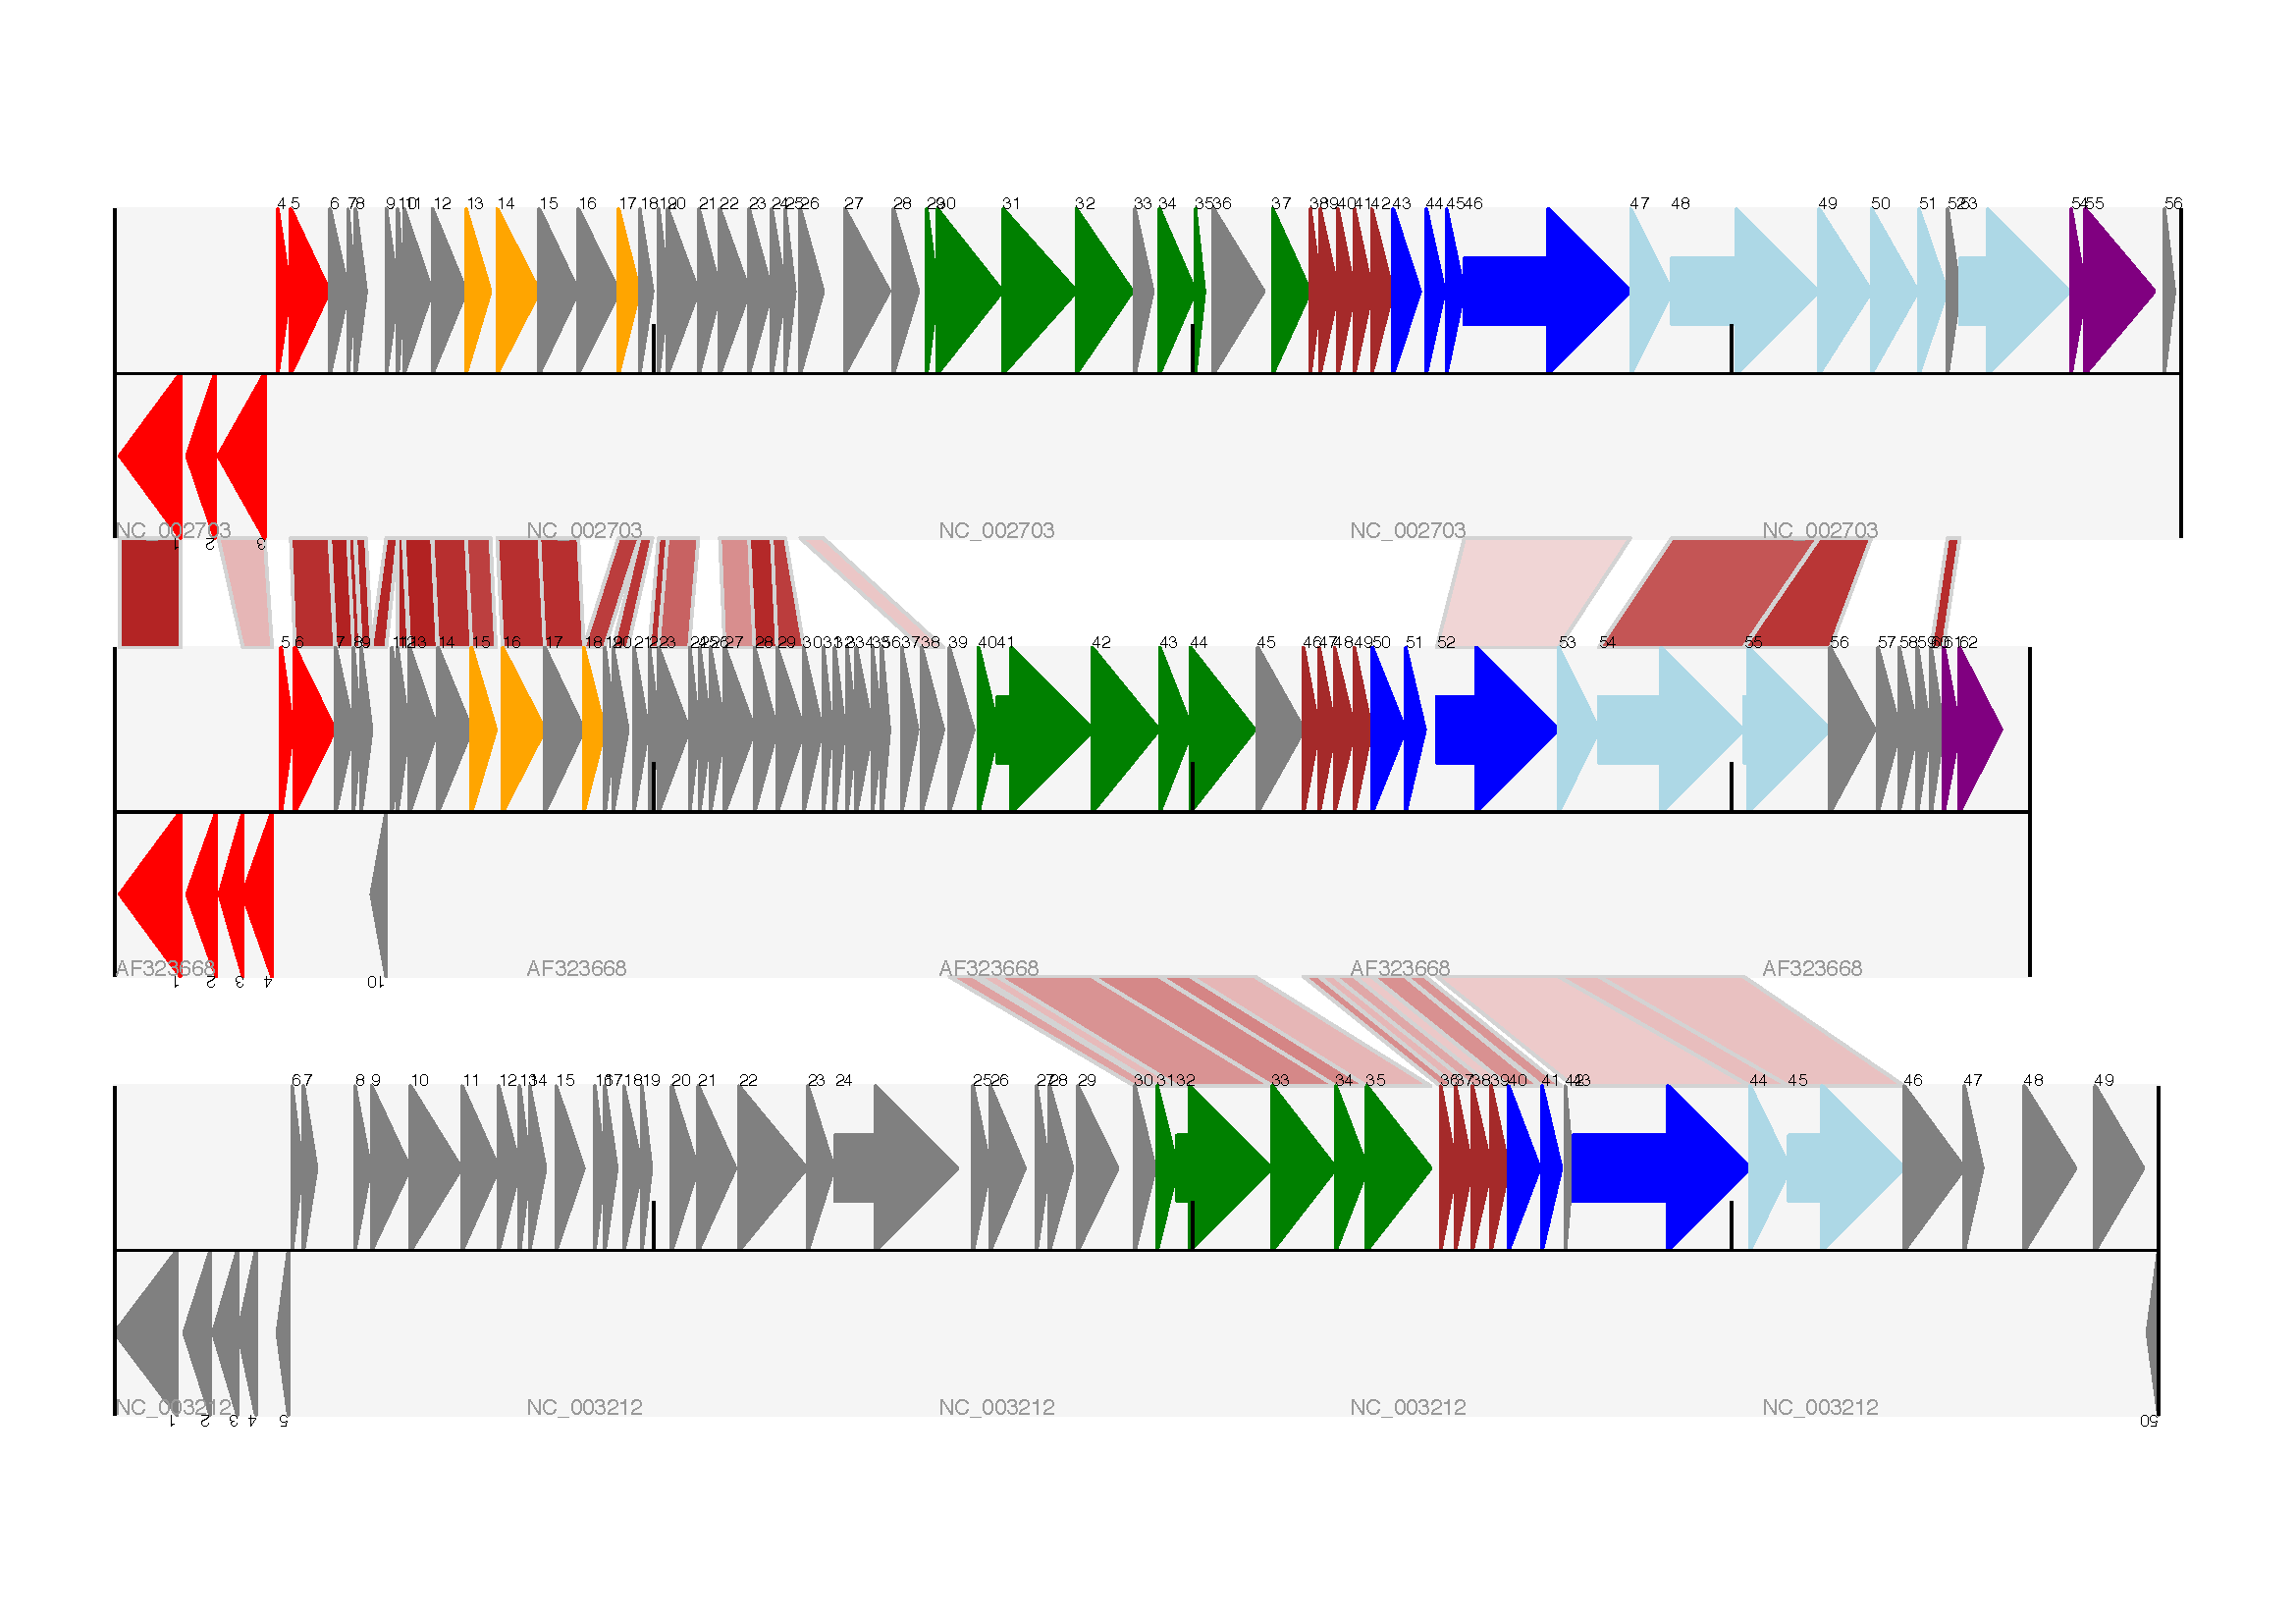
\includegraphics{three_track_cl.png}

当然,Biopython还有很多增强图像效果的方法。首先,这个示例中的cross links是蛋白质之间的,被呈现在一个链的固定区域(strand specific manor)。可以在feature track上用 ‘BOX’ sigil添加背景区域(background region)来扩展cross link的效果。同样,可以缩短feature tracks之间的垂直高度,使用更多的links来代替——一种方法是为空的track分配空间。此外,在没有大规模基因重叠的情况下,可以用跨越轴线的''BIGARROW'',这样就为track进一步增加了垂直空间。详情请查看Biopython源程序的 \code{Doc/examples} 目录下的示例脚本文件:\href{http://biopython.org/SRC/biopython/Doc/examples/Proux\_et\_al\_2002\_Figure\_6.py}{Proux\_et\_al\_2002\_Figure\_6.py} 。
结果见下图:

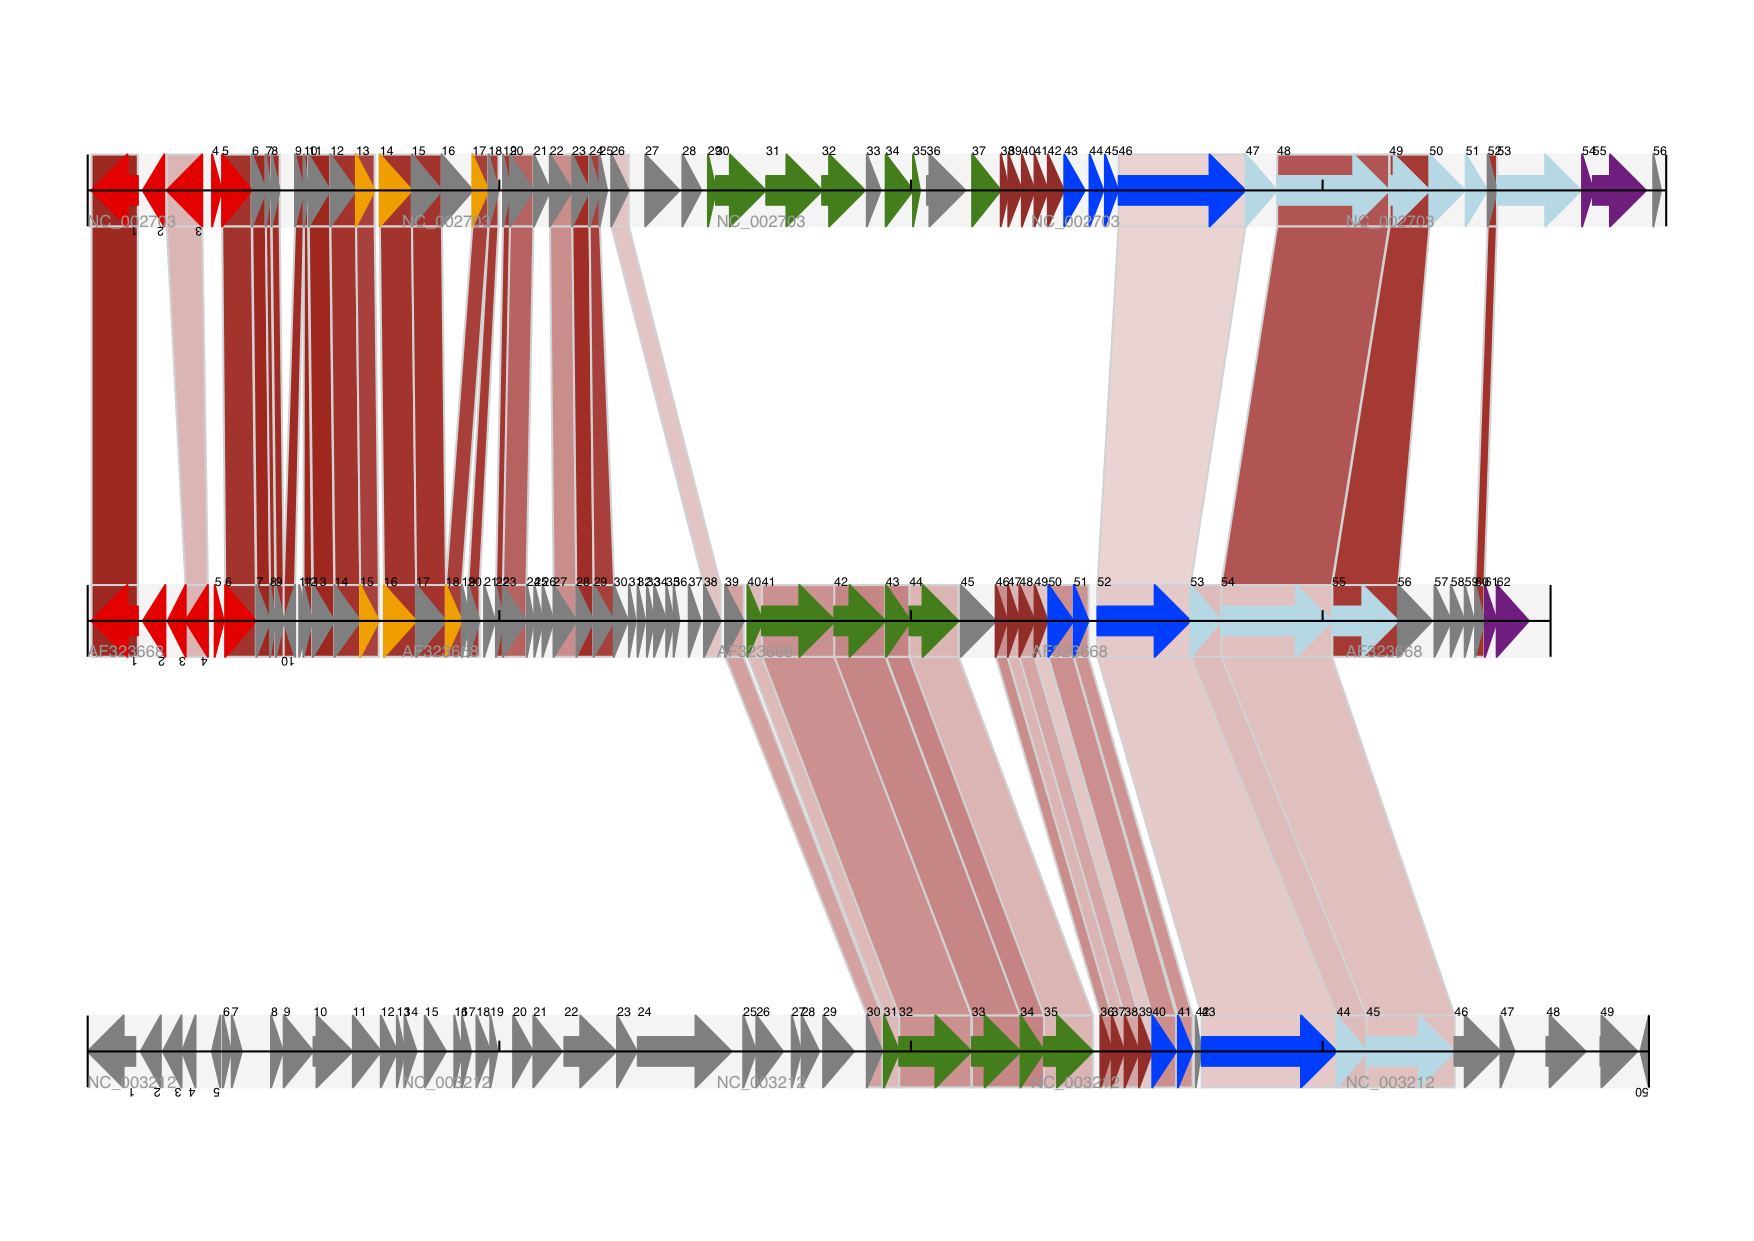
\includegraphics{three_track_cl2a.png}

除此之外,你可能希望在图像编辑软件里手动调整gene标签的位置,添加特定标识,比如强调某个特别的区域。

如果有多个叠加的links,使用ReportLab库里的颜色透明度(transparent color)是非常好的方法,由于这个示例没有cross-link的重叠,所以没有用到颜色透明度(transparent color)。然而,尽量避免在这个示例中使用边框阴影(shaded color scheme)。


\subsection{17.1.12 高级选项}
\label{chr17:id10}
可以通过控制刻度线(tick marks)来调节展示比例(scale),毕竟每个图形应该包括基本单位和轴线标签的数目。

到目前为止,我们只使用了 \code{FeatureSet} 。GenomeDiagram还可以用 \code{GraphSet} 来制作线形图,饼状图和heatmap热图(例如在轨迹内展示feature中的GC含量)。

目前还没有添加这个选项,最后,推荐你去参考GenomeDiagram单机版 \href{http://biopython.org/DIST/docs/GenomeDiagram/userguide.pdf}{用户指南
(PDF)} 和文档字符串(docstrings)。


\subsection{17.1.13 转换旧代码}
\label{chr17:id11}
如果你有用GenomeDiagram独立版本写的旧代码,想将其转换为Bippython和新版本可识别的代码,你需要做一些调整——主要是import语句。GenomeDiagram的旧版本中使用英式拼写“colour” 和 “centre”来表示“color” 和“center”。被Biopython整合后,参数名可以使用任意一种。但是将来可能会不支持英式的参数名。

如果你过去使用下面的方式:
\DUspan{keyword,namespace}{}\DUspan{name,namespace}{}\DUspan{keyword,namespace}{}\DUspan{name}{}\DUspan{punctuation}{}\DUspan{name}{}\DUspan{name}{}\DUspan{operator}{}\DUspan{name}{}\DUspan{punctuation}{}\DUspan{literal,string}{}\DUspan{punctuation}{}\DUspan{operator}{}
\begin{Verbatim}[commandchars=\\\{\}]
\PYG{k+kn}{from} \PYG{n+nn}{GenomeDiagram} \PYG{k+kn}{import} \PYG{n}{GDFeatureSet}\PYG{p}{,} \PYG{n}{GDDiagram}
\PYG{n}{gdd} \PYG{o}{=} \PYG{n}{GDDiagram}\PYG{p}{(}\PYG{l+s}{\PYGZdq{}}\PYG{l+s}{An example}\PYG{l+s}{\PYGZdq{}}\PYG{p}{)}
\PYG{o}{.}\PYG{o}{.}\PYG{o}{.}
\end{Verbatim}

你只需要将import语句转换成下面这样:
\DUspan{keyword,namespace}{}\DUspan{name,namespace}{}\DUspan{keyword,namespace}{}\DUspan{name}{}\DUspan{keyword}{}\DUspan{name}{}\DUspan{punctuation}{}\DUspan{name}{}\DUspan{keyword}{}\DUspan{name}{}\DUspan{name}{}\DUspan{operator}{}\DUspan{name}{}\DUspan{punctuation}{}\DUspan{literal,string}{}\DUspan{punctuation}{}\DUspan{operator}{}
\begin{Verbatim}[commandchars=\\\{\}]
\PYG{k+kn}{from} \PYG{n+nn}{Bio.Graphics.GenomeDiagram} \PYG{k+kn}{import} \PYG{n}{FeatureSet} \PYG{k}{as} \PYG{n}{GDFeatureSet}\PYG{p}{,} \PYG{n}{Diagram} \PYG{k}{as} \PYG{n}{GDDiagram}
\PYG{n}{gdd} \PYG{o}{=} \PYG{n}{GDDiagram}\PYG{p}{(}\PYG{l+s}{\PYGZdq{}}\PYG{l+s}{An example}\PYG{l+s}{\PYGZdq{}}\PYG{p}{)}
\PYG{o}{.}\PYG{o}{.}\PYG{o}{.}
\end{Verbatim}

希望能够顺利运行。将来你可能想换用新名称,你必须在更大程度上改变你编写代码的方式:
\DUspan{keyword,namespace}{}\DUspan{name,namespace}{}\DUspan{keyword,namespace}{}\DUspan{name}{}\DUspan{punctuation}{}\DUspan{name}{}\DUspan{name}{}\DUspan{operator}{}\DUspan{name}{}\DUspan{punctuation}{}\DUspan{literal,string}{}\DUspan{punctuation}{}\DUspan{operator}{}
\begin{Verbatim}[commandchars=\\\{\}]
\PYG{k+kn}{from} \PYG{n+nn}{Bio.Graphics.GenomeDiagram} \PYG{k+kn}{import} \PYG{n}{FeatureSet}\PYG{p}{,} \PYG{n}{Diagram}
\PYG{n}{gdd} \PYG{o}{=} \PYG{n}{Diagram}\PYG{p}{(}\PYG{l+s}{\PYGZdq{}}\PYG{l+s}{An example}\PYG{l+s}{\PYGZdq{}}\PYG{p}{)}
\PYG{o}{.}\PYG{o}{.}\PYG{o}{.}
\end{Verbatim}

or:
\DUspan{keyword,namespace}{}\DUspan{name,namespace}{}\DUspan{keyword,namespace}{}\DUspan{name}{}\DUspan{name}{}\DUspan{operator}{}\DUspan{name}{}\DUspan{operator}{}\DUspan{name}{}\DUspan{punctuation}{}\DUspan{literal,string}{}\DUspan{punctuation}{}\DUspan{operator}{}
\begin{Verbatim}[commandchars=\\\{\}]
\PYG{k+kn}{from} \PYG{n+nn}{Bio.Graphics} \PYG{k+kn}{import} \PYG{n}{GenomeDiagram}
\PYG{n}{gdd} \PYG{o}{=} \PYG{n}{GenomeDiagram}\PYG{o}{.}\PYG{n}{Diagram}\PYG{p}{(}\PYG{l+s}{\PYGZdq{}}\PYG{l+s}{An example}\PYG{l+s}{\PYGZdq{}}\PYG{p}{)}
\PYG{o}{.}\PYG{o}{.}\PYG{o}{.}
\end{Verbatim}

如果运行过程中出现问题,请到Biopython邮件列表中寻求帮助。唯一的缺点就是没有包括旧模块 \code{GenomeDiagram.GDUtilities} ,这个模块有计算GC百分比含量的函数,这一部分将会合并到 \code{Bio.SeqUtils} 模块。


\section{17.2 染色体}
\label{chr17:id12}
\code{Bio.Graphics.BasicChromosome} 模块可以绘制染色体,Jupe等人在2012发表的文章 {[}{\hyperref[chr23:jupe2012]{\emph{6}}}{]} 中利用不同的颜色来展示不同的基因家族。


\subsection{17.2.1 简单染色体}
\label{chr17:id13}
我们用 \emph{Arabidopsis
thaliana} 来展示一个简单示例。

首先从NCBI的FTP服务器 \href{ftp://ftp.ncbi.nlm.nih.gov/genomes/Arabidopsis\_thaliana}{ftp://ftp.ncbi.nlm.nih.gov/genomes/Arabidopsis\_thaliana} 下载拟南芥已测序的五个染色体文件,利用 \code{Bio.SeqIO} 函数计算它们的长度。你可以利用GenBank文件,但是对于染色体来说,FASTA文件的处理速度会快点。
\DUspan{keyword,namespace}{}\DUspan{name,namespace}{}\DUspan{keyword,namespace}{}\DUspan{name}{}\DUspan{name}{}\DUspan{operator}{}\DUspan{punctuation}{}\DUspan{literal,string}{}\DUspan{punctuation}{}\DUspan{literal,string}{}\DUspan{punctuation}{}\DUspan{punctuation}{}\DUspan{literal,string}{}\DUspan{punctuation}{}\DUspan{literal,string}{}\DUspan{punctuation}{}\DUspan{punctuation}{}\DUspan{literal,string}{}\DUspan{punctuation}{}\DUspan{literal,string}{}\DUspan{punctuation}{}\DUspan{punctuation}{}\DUspan{literal,string}{}\DUspan{punctuation}{}\DUspan{literal,string}{}\DUspan{punctuation}{}\DUspan{punctuation}{}\DUspan{literal,string}{}\DUspan{punctuation}{}\DUspan{literal,string}{}\DUspan{punctuation}{}\DUspan{keyword}{}\DUspan{punctuation}{}\DUspan{name}{}\DUspan{punctuation}{}\DUspan{name}{}\DUspan{punctuation}{}\DUspan{operator,word}{}\DUspan{name}{}\DUspan{punctuation}{}\DUspan{name}{}\DUspan{operator}{}\DUspan{name}{}\DUspan{operator}{}\DUspan{name}{}\DUspan{punctuation}{}\DUspan{name}{}\DUspan{punctuation}{}\DUspan{literal,string}{}\DUspan{punctuation}{}\DUspan{keyword}{}\DUspan{name}{}\DUspan{punctuation}{}\DUspan{name,builtin}{}\DUspan{punctuation}{}\DUspan{name}{}\DUspan{punctuation}{}
\begin{Verbatim}[commandchars=\\\{\}]
\PYG{k+kn}{from} \PYG{n+nn}{Bio} \PYG{k+kn}{import} \PYG{n}{SeqIO}
\PYG{n}{entries} \PYG{o}{=} \PYG{p}{[}\PYG{p}{(}\PYG{l+s}{\PYGZdq{}}\PYG{l+s}{Chr I}\PYG{l+s}{\PYGZdq{}}\PYG{p}{,} \PYG{l+s}{\PYGZdq{}}\PYG{l+s}{CHR\PYGZus{}I/NC\PYGZus{}003070.fna}\PYG{l+s}{\PYGZdq{}}\PYG{p}{)}\PYG{p}{,}
           \PYG{p}{(}\PYG{l+s}{\PYGZdq{}}\PYG{l+s}{Chr II}\PYG{l+s}{\PYGZdq{}}\PYG{p}{,} \PYG{l+s}{\PYGZdq{}}\PYG{l+s}{CHR\PYGZus{}II/NC\PYGZus{}003071.fna}\PYG{l+s}{\PYGZdq{}}\PYG{p}{)}\PYG{p}{,}
           \PYG{p}{(}\PYG{l+s}{\PYGZdq{}}\PYG{l+s}{Chr III}\PYG{l+s}{\PYGZdq{}}\PYG{p}{,} \PYG{l+s}{\PYGZdq{}}\PYG{l+s}{CHR\PYGZus{}III/NC\PYGZus{}003074.fna}\PYG{l+s}{\PYGZdq{}}\PYG{p}{)}\PYG{p}{,}
           \PYG{p}{(}\PYG{l+s}{\PYGZdq{}}\PYG{l+s}{Chr IV}\PYG{l+s}{\PYGZdq{}}\PYG{p}{,} \PYG{l+s}{\PYGZdq{}}\PYG{l+s}{CHR\PYGZus{}IV/NC\PYGZus{}003075.fna}\PYG{l+s}{\PYGZdq{}}\PYG{p}{)}\PYG{p}{,}
           \PYG{p}{(}\PYG{l+s}{\PYGZdq{}}\PYG{l+s}{Chr V}\PYG{l+s}{\PYGZdq{}}\PYG{p}{,} \PYG{l+s}{\PYGZdq{}}\PYG{l+s}{CHR\PYGZus{}V/NC\PYGZus{}003076.fna}\PYG{l+s}{\PYGZdq{}}\PYG{p}{)}\PYG{p}{]}
\PYG{k}{for} \PYG{p}{(}\PYG{n}{name}\PYG{p}{,} \PYG{n}{filename}\PYG{p}{)} \PYG{o+ow}{in} \PYG{n}{entries}\PYG{p}{:}
   \PYG{n}{record} \PYG{o}{=} \PYG{n}{SeqIO}\PYG{o}{.}\PYG{n}{read}\PYG{p}{(}\PYG{n}{filename}\PYG{p}{,}\PYG{l+s}{\PYGZdq{}}\PYG{l+s}{fasta}\PYG{l+s}{\PYGZdq{}}\PYG{p}{)}
   \PYG{k}{print} \PYG{n}{name}\PYG{p}{,} \PYG{n+nb}{len}\PYG{p}{(}\PYG{n}{record}\PYG{p}{)}
\end{Verbatim}

计算出5个染色体长度后,就可用 \code{BasicChromosome} 模块对其作如下的处理:
\DUspan{keyword,namespace}{}\DUspan{name,namespace}{}\DUspan{keyword,namespace}{}\DUspan{name}{}\DUspan{keyword,namespace}{}\DUspan{name,namespace}{}\DUspan{keyword,namespace}{}\DUspan{name}{}\DUspan{name}{}\DUspan{operator}{}\DUspan{punctuation}{}\DUspan{literal,string}{}\DUspan{punctuation}{}\DUspan{literal,number,integer}{}\DUspan{punctuation}{}\DUspan{punctuation}{}\DUspan{literal,string}{}\DUspan{punctuation}{}\DUspan{literal,number,integer}{}\DUspan{punctuation}{}\DUspan{punctuation}{}\DUspan{literal,string}{}\DUspan{punctuation}{}\DUspan{literal,number,integer}{}\DUspan{punctuation}{}\DUspan{punctuation}{}\DUspan{literal,string}{}\DUspan{punctuation}{}\DUspan{literal,number,integer}{}\DUspan{punctuation}{}\DUspan{punctuation}{}\DUspan{literal,string}{}\DUspan{punctuation}{}\DUspan{literal,number,integer}{}\DUspan{punctuation}{}\DUspan{name}{}\DUspan{operator}{}\DUspan{literal,number,integer}{}\DUspan{comment}{}\DUspan{name}{}\DUspan{operator}{}\DUspan{literal,number,integer}{}\DUspan{comment}{}\DUspan{name}{}\DUspan{operator}{}\DUspan{name}{}\DUspan{operator}{}\DUspan{name}{}\DUspan{punctuation}{}\DUspan{name}{}\DUspan{operator}{}\DUspan{name}{}\DUspan{operator}{}\DUspan{punctuation}{}\DUspan{literal,number,float}{}\DUspan{operator}{}\DUspan{name}{}\DUspan{punctuation}{}\DUspan{literal,number,integer}{}\DUspan{operator}{}\DUspan{name}{}\DUspan{punctuation}{}\DUspan{comment}{}\DUspan{keyword}{}\DUspan{name}{}\DUspan{punctuation}{}\DUspan{name}{}\DUspan{operator,word}{}\DUspan{name}{}\DUspan{punctuation}{}\DUspan{name}{}\DUspan{operator}{}\DUspan{name}{}\DUspan{operator}{}\DUspan{name}{}\DUspan{punctuation}{}\DUspan{name}{}\DUspan{punctuation}{}\DUspan{comment}{}\DUspan{comment}{}\DUspan{comment}{}\DUspan{name}{}\DUspan{operator}{}\DUspan{name}{}\DUspan{operator}{}\DUspan{name}{}\DUspan{operator}{}\DUspan{literal,number,integer}{}\DUspan{operator}{}\DUspan{name}{}\DUspan{comment}{}\DUspan{name}{}\DUspan{operator}{}\DUspan{name}{}\DUspan{operator}{}\DUspan{name}{}\DUspan{punctuation}{}\DUspan{name}{}\DUspan{operator}{}\DUspan{name}{}\DUspan{operator}{}\DUspan{name}{}\DUspan{name}{}\DUspan{operator}{}\DUspan{name}{}\DUspan{punctuation}{}\DUspan{name}{}\DUspan{punctuation}{}\DUspan{comment}{}\DUspan{name}{}\DUspan{operator}{}\DUspan{name}{}\DUspan{operator}{}\DUspan{name}{}\DUspan{punctuation}{}\DUspan{name}{}\DUspan{operator}{}\DUspan{name}{}\DUspan{operator}{}\DUspan{name}{}\DUspan{name}{}\DUspan{operator}{}\DUspan{name}{}\DUspan{punctuation}{}\DUspan{name}{}\DUspan{punctuation}{}\DUspan{comment}{}\DUspan{name}{}\DUspan{operator}{}\DUspan{name}{}\DUspan{operator}{}\DUspan{name}{}\DUspan{punctuation}{}\DUspan{name}{}\DUspan{operator}{}\DUspan{name,builtin,pseudo}{}\DUspan{punctuation}{}\DUspan{name}{}\DUspan{operator}{}\DUspan{name}{}\DUspan{operator}{}\DUspan{name}{}\DUspan{name}{}\DUspan{operator}{}\DUspan{name}{}\DUspan{punctuation}{}\DUspan{name}{}\DUspan{punctuation}{}\DUspan{comment}{}\DUspan{name}{}\DUspan{operator}{}\DUspan{name}{}\DUspan{punctuation}{}\DUspan{name}{}\DUspan{punctuation}{}\DUspan{name}{}\DUspan{operator}{}\DUspan{name}{}\DUspan{punctuation}{}\DUspan{literal,string}{}\DUspan{punctuation}{}\DUspan{literal,string}{}\DUspan{punctuation}{}
\begin{Verbatim}[commandchars=\\\{\}]
\PYG{k+kn}{from} \PYG{n+nn}{reportlab.lib.units} \PYG{k+kn}{import} \PYG{n}{cm}
\PYG{k+kn}{from} \PYG{n+nn}{Bio.Graphics} \PYG{k+kn}{import} \PYG{n}{BasicChromosome}

\PYG{n}{entries} \PYG{o}{=} \PYG{p}{[}\PYG{p}{(}\PYG{l+s}{\PYGZdq{}}\PYG{l+s}{Chr I}\PYG{l+s}{\PYGZdq{}}\PYG{p}{,} \PYG{l+m+mi}{30432563}\PYG{p}{)}\PYG{p}{,}
           \PYG{p}{(}\PYG{l+s}{\PYGZdq{}}\PYG{l+s}{Chr II}\PYG{l+s}{\PYGZdq{}}\PYG{p}{,} \PYG{l+m+mi}{19705359}\PYG{p}{)}\PYG{p}{,}
           \PYG{p}{(}\PYG{l+s}{\PYGZdq{}}\PYG{l+s}{Chr III}\PYG{l+s}{\PYGZdq{}}\PYG{p}{,} \PYG{l+m+mi}{23470805}\PYG{p}{)}\PYG{p}{,}
           \PYG{p}{(}\PYG{l+s}{\PYGZdq{}}\PYG{l+s}{Chr IV}\PYG{l+s}{\PYGZdq{}}\PYG{p}{,} \PYG{l+m+mi}{18585042}\PYG{p}{)}\PYG{p}{,}
           \PYG{p}{(}\PYG{l+s}{\PYGZdq{}}\PYG{l+s}{Chr V}\PYG{l+s}{\PYGZdq{}}\PYG{p}{,} \PYG{l+m+mi}{26992728}\PYG{p}{)}\PYG{p}{]}

\PYG{n}{max\PYGZus{}len} \PYG{o}{=} \PYG{l+m+mi}{30432563} \PYG{c}{\PYGZsh{}Could compute this}
\PYG{n}{telomere\PYGZus{}length} \PYG{o}{=} \PYG{l+m+mi}{1000000} \PYG{c}{\PYGZsh{}For illustration}

\PYG{n}{chr\PYGZus{}diagram} \PYG{o}{=} \PYG{n}{BasicChromosome}\PYG{o}{.}\PYG{n}{Organism}\PYG{p}{(}\PYG{p}{)}
\PYG{n}{chr\PYGZus{}diagram}\PYG{o}{.}\PYG{n}{page\PYGZus{}size} \PYG{o}{=} \PYG{p}{(}\PYG{l+m+mf}{29.7}\PYG{o}{*}\PYG{n}{cm}\PYG{p}{,} \PYG{l+m+mi}{21}\PYG{o}{*}\PYG{n}{cm}\PYG{p}{)} \PYG{c}{\PYGZsh{}A4 landscape}

\PYG{k}{for} \PYG{n}{name}\PYG{p}{,} \PYG{n}{length} \PYG{o+ow}{in} \PYG{n}{entries}\PYG{p}{:}
    \PYG{n}{cur\PYGZus{}chromosome} \PYG{o}{=} \PYG{n}{BasicChromosome}\PYG{o}{.}\PYG{n}{Chromosome}\PYG{p}{(}\PYG{n}{name}\PYG{p}{)}
    \PYG{c}{\PYGZsh{}Set the scale to the MAXIMUM length plus the two telomeres in bp,}
    \PYG{c}{\PYGZsh{}want the same scale used on all five chromosomes so they can be}
    \PYG{c}{\PYGZsh{}compared to each other}
    \PYG{n}{cur\PYGZus{}chromosome}\PYG{o}{.}\PYG{n}{scale\PYGZus{}num} \PYG{o}{=} \PYG{n}{max\PYGZus{}len} \PYG{o}{+} \PYG{l+m+mi}{2} \PYG{o}{*} \PYG{n}{telomere\PYGZus{}length}

    \PYG{c}{\PYGZsh{}Add an opening telomere}
    \PYG{n}{start} \PYG{o}{=} \PYG{n}{BasicChromosome}\PYG{o}{.}\PYG{n}{TelomereSegment}\PYG{p}{(}\PYG{p}{)}
    \PYG{n}{start}\PYG{o}{.}\PYG{n}{scale} \PYG{o}{=} \PYG{n}{telomere\PYGZus{}length}
    \PYG{n}{cur\PYGZus{}chromosome}\PYG{o}{.}\PYG{n}{add}\PYG{p}{(}\PYG{n}{start}\PYG{p}{)}

    \PYG{c}{\PYGZsh{}Add a body \PYGZhy{} using bp as the scale length here.}
    \PYG{n}{body} \PYG{o}{=} \PYG{n}{BasicChromosome}\PYG{o}{.}\PYG{n}{ChromosomeSegment}\PYG{p}{(}\PYG{p}{)}
    \PYG{n}{body}\PYG{o}{.}\PYG{n}{scale} \PYG{o}{=} \PYG{n}{length}
    \PYG{n}{cur\PYGZus{}chromosome}\PYG{o}{.}\PYG{n}{add}\PYG{p}{(}\PYG{n}{body}\PYG{p}{)}

    \PYG{c}{\PYGZsh{}Add a closing telomere}
    \PYG{n}{end} \PYG{o}{=} \PYG{n}{BasicChromosome}\PYG{o}{.}\PYG{n}{TelomereSegment}\PYG{p}{(}\PYG{n}{inverted}\PYG{o}{=}\PYG{n+nb+bp}{True}\PYG{p}{)}
    \PYG{n}{end}\PYG{o}{.}\PYG{n}{scale} \PYG{o}{=} \PYG{n}{telomere\PYGZus{}length}
    \PYG{n}{cur\PYGZus{}chromosome}\PYG{o}{.}\PYG{n}{add}\PYG{p}{(}\PYG{n}{end}\PYG{p}{)}

    \PYG{c}{\PYGZsh{}This chromosome is done}
    \PYG{n}{chr\PYGZus{}diagram}\PYG{o}{.}\PYG{n}{add}\PYG{p}{(}\PYG{n}{cur\PYGZus{}chromosome}\PYG{p}{)}

\PYG{n}{chr\PYGZus{}diagram}\PYG{o}{.}\PYG{n}{draw}\PYG{p}{(}\PYG{l+s}{\PYGZdq{}}\PYG{l+s}{simple\PYGZus{}chrom.pdf}\PYG{l+s}{\PYGZdq{}}\PYG{p}{,} \PYG{l+s}{\PYGZdq{}}\PYG{l+s}{Arabidopsis thaliana}\PYG{l+s}{\PYGZdq{}}\PYG{p}{)}
\end{Verbatim}

新建的PDF文档如图所示:

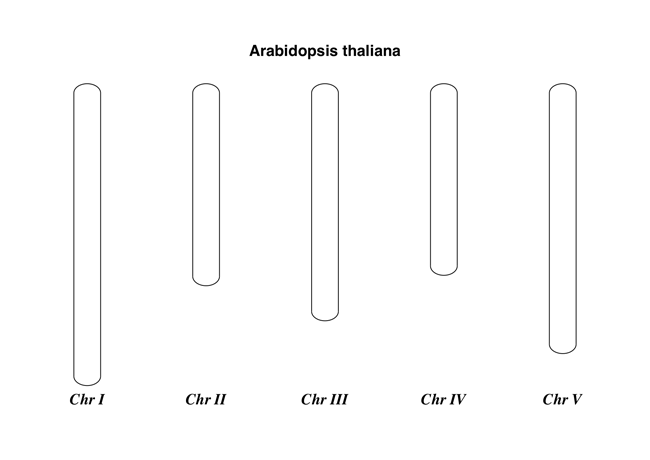
\includegraphics{simple_chrom.png}

这个示例可以短小精悍,下面的示例可以展示目标feature的定位。


\subsection{17.2.2 染色体注释}
\label{chr17:id14}
继续前面的示例,我们可以同时展示tRNA基因。通过解析 \emph{Arabidopsis thaliana} 的5个染色体GenBank文件,我们可以对他们进行定位。你需要从NCBI的FTP服务器下载这些文件 \href{ftp://ftp.ncbi.nlm.nih.gov/genomes/Arabidopsis\_thaliana}{ftp://ftp.ncbi.nlm.nih.gov/genomes/Arabidopsis\_thaliana} ,也可以保存子目录名称或者添加如下的路径:
\DUspan{keyword,namespace}{}\DUspan{name,namespace}{}\DUspan{keyword,namespace}{}\DUspan{name}{}\DUspan{keyword,namespace}{}\DUspan{name,namespace}{}\DUspan{keyword,namespace}{}\DUspan{name}{}\DUspan{keyword,namespace}{}\DUspan{name,namespace}{}\DUspan{keyword,namespace}{}\DUspan{name}{}\DUspan{name}{}\DUspan{operator}{}\DUspan{punctuation}{}\DUspan{literal,string}{}\DUspan{punctuation}{}\DUspan{literal,string}{}\DUspan{punctuation}{}\DUspan{punctuation}{}\DUspan{literal,string}{}\DUspan{punctuation}{}\DUspan{literal,string}{}\DUspan{punctuation}{}\DUspan{punctuation}{}\DUspan{literal,string}{}\DUspan{punctuation}{}\DUspan{literal,string}{}\DUspan{punctuation}{}\DUspan{punctuation}{}\DUspan{literal,string}{}\DUspan{punctuation}{}\DUspan{literal,string}{}\DUspan{punctuation}{}\DUspan{punctuation}{}\DUspan{literal,string}{}\DUspan{punctuation}{}\DUspan{literal,string}{}\DUspan{punctuation}{}\DUspan{name}{}\DUspan{operator}{}\DUspan{literal,number,integer}{}\DUspan{comment}{}\DUspan{name}{}\DUspan{operator}{}\DUspan{literal,number,integer}{}\DUspan{comment}{}\DUspan{name}{}\DUspan{operator}{}\DUspan{name}{}\DUspan{operator}{}\DUspan{name}{}\DUspan{punctuation}{}\DUspan{name}{}\DUspan{operator}{}\DUspan{name}{}\DUspan{operator}{}\DUspan{punctuation}{}\DUspan{literal,number,float}{}\DUspan{operator}{}\DUspan{name}{}\DUspan{punctuation}{}\DUspan{literal,number,integer}{}\DUspan{operator}{}\DUspan{name}{}\DUspan{punctuation}{}\DUspan{comment}{}\DUspan{keyword}{}\DUspan{name}{}\DUspan{punctuation}{}\DUspan{punctuation}{}\DUspan{name}{}\DUspan{punctuation}{}\DUspan{name}{}\DUspan{punctuation}{}\DUspan{operator,word}{}\DUspan{name,builtin}{}\DUspan{punctuation}{}\DUspan{name}{}\DUspan{punctuation}{}\DUspan{name}{}\DUspan{operator}{}\DUspan{name}{}\DUspan{operator}{}\DUspan{name}{}\DUspan{punctuation}{}\DUspan{name}{}\DUspan{punctuation}{}\DUspan{literal,string}{}\DUspan{punctuation}{}\DUspan{name}{}\DUspan{operator}{}\DUspan{name,builtin}{}\DUspan{punctuation}{}\DUspan{name}{}\DUspan{punctuation}{}\DUspan{name}{}\DUspan{operator}{}\DUspan{punctuation}{}\DUspan{name}{}\DUspan{keyword}{}\DUspan{name}{}\DUspan{operator,word}{}\DUspan{name}{}\DUspan{operator}{}\DUspan{name}{}\DUspan{keyword}{}\DUspan{name}{}\DUspan{operator}{}\DUspan{name}{}\DUspan{operator}{}\DUspan{literal,string}{}\DUspan{punctuation}{}\DUspan{comment}{}\DUspan{comment}{}\DUspan{keyword}{}\DUspan{name}{}\DUspan{operator,word}{}\DUspan{name}{}\DUspan{punctuation}{}\DUspan{name}{}\DUspan{operator}{}\DUspan{name}{}\DUspan{punctuation}{}\DUspan{literal,string}{}\DUspan{punctuation}{}\DUspan{operator}{}\DUspan{punctuation}{}\DUspan{name}{}\DUspan{operator}{}\DUspan{literal,number,integer}{}\DUspan{punctuation}{}\DUspan{name}{}\DUspan{operator}{}\DUspan{name}{}\DUspan{operator}{}\DUspan{name}{}\DUspan{punctuation}{}\DUspan{name}{}\DUspan{punctuation}{}\DUspan{comment}{}\DUspan{comment}{}\DUspan{comment}{}\DUspan{name}{}\DUspan{operator}{}\DUspan{name}{}\DUspan{operator}{}\DUspan{name}{}\DUspan{operator}{}\DUspan{literal,number,integer}{}\DUspan{operator}{}\DUspan{name}{}\DUspan{comment}{}\DUspan{name}{}\DUspan{operator}{}\DUspan{name}{}\DUspan{operator}{}\DUspan{name}{}\DUspan{punctuation}{}\DUspan{name}{}\DUspan{operator}{}\DUspan{name}{}\DUspan{operator}{}\DUspan{name}{}\DUspan{name}{}\DUspan{operator}{}\DUspan{name}{}\DUspan{punctuation}{}\DUspan{name}{}\DUspan{punctuation}{}\DUspan{comment}{}\DUspan{name}{}\DUspan{operator}{}\DUspan{name}{}\DUspan{operator}{}\DUspan{name}{}\DUspan{punctuation}{}\DUspan{name}{}\DUspan{punctuation}{}\DUspan{name}{}\DUspan{punctuation}{}\DUspan{name}{}\DUspan{operator}{}\DUspan{name}{}\DUspan{operator}{}\DUspan{name}{}\DUspan{name}{}\DUspan{operator}{}\DUspan{name}{}\DUspan{punctuation}{}\DUspan{name}{}\DUspan{punctuation}{}\DUspan{comment}{}\DUspan{name}{}\DUspan{operator}{}\DUspan{name}{}\DUspan{operator}{}\DUspan{name}{}\DUspan{punctuation}{}\DUspan{name}{}\DUspan{operator}{}\DUspan{name,builtin,pseudo}{}\DUspan{punctuation}{}\DUspan{name}{}\DUspan{operator}{}\DUspan{name}{}\DUspan{operator}{}\DUspan{name}{}\DUspan{name}{}\DUspan{operator}{}\DUspan{name}{}\DUspan{punctuation}{}\DUspan{name}{}\DUspan{punctuation}{}\DUspan{comment}{}\DUspan{name}{}\DUspan{operator}{}\DUspan{name}{}\DUspan{punctuation}{}\DUspan{name}{}\DUspan{punctuation}{}\DUspan{name}{}\DUspan{operator}{}\DUspan{name}{}\DUspan{punctuation}{}\DUspan{literal,string}{}\DUspan{punctuation}{}\DUspan{literal,string}{}\DUspan{punctuation}{}
\begin{Verbatim}[commandchars=\\\{\}]
\PYG{k+kn}{from} \PYG{n+nn}{reportlab.lib.units} \PYG{k+kn}{import} \PYG{n}{cm}
\PYG{k+kn}{from} \PYG{n+nn}{Bio} \PYG{k+kn}{import} \PYG{n}{SeqIO}
\PYG{k+kn}{from} \PYG{n+nn}{Bio.Graphics} \PYG{k+kn}{import} \PYG{n}{BasicChromosome}

\PYG{n}{entries} \PYG{o}{=} \PYG{p}{[}\PYG{p}{(}\PYG{l+s}{\PYGZdq{}}\PYG{l+s}{Chr I}\PYG{l+s}{\PYGZdq{}}\PYG{p}{,} \PYG{l+s}{\PYGZdq{}}\PYG{l+s}{CHR\PYGZus{}I/NC\PYGZus{}003070.gbk}\PYG{l+s}{\PYGZdq{}}\PYG{p}{)}\PYG{p}{,}
           \PYG{p}{(}\PYG{l+s}{\PYGZdq{}}\PYG{l+s}{Chr II}\PYG{l+s}{\PYGZdq{}}\PYG{p}{,} \PYG{l+s}{\PYGZdq{}}\PYG{l+s}{CHR\PYGZus{}II/NC\PYGZus{}003071.gbk}\PYG{l+s}{\PYGZdq{}}\PYG{p}{)}\PYG{p}{,}
           \PYG{p}{(}\PYG{l+s}{\PYGZdq{}}\PYG{l+s}{Chr III}\PYG{l+s}{\PYGZdq{}}\PYG{p}{,} \PYG{l+s}{\PYGZdq{}}\PYG{l+s}{CHR\PYGZus{}III/NC\PYGZus{}003074.gbk}\PYG{l+s}{\PYGZdq{}}\PYG{p}{)}\PYG{p}{,}
           \PYG{p}{(}\PYG{l+s}{\PYGZdq{}}\PYG{l+s}{Chr IV}\PYG{l+s}{\PYGZdq{}}\PYG{p}{,} \PYG{l+s}{\PYGZdq{}}\PYG{l+s}{CHR\PYGZus{}IV/NC\PYGZus{}003075.gbk}\PYG{l+s}{\PYGZdq{}}\PYG{p}{)}\PYG{p}{,}
           \PYG{p}{(}\PYG{l+s}{\PYGZdq{}}\PYG{l+s}{Chr V}\PYG{l+s}{\PYGZdq{}}\PYG{p}{,} \PYG{l+s}{\PYGZdq{}}\PYG{l+s}{CHR\PYGZus{}V/NC\PYGZus{}003076.gbk}\PYG{l+s}{\PYGZdq{}}\PYG{p}{)}\PYG{p}{]}

\PYG{n}{max\PYGZus{}len} \PYG{o}{=} \PYG{l+m+mi}{30432563} \PYG{c}{\PYGZsh{}Could compute this}
\PYG{n}{telomere\PYGZus{}length} \PYG{o}{=} \PYG{l+m+mi}{1000000} \PYG{c}{\PYGZsh{}For illustration}

\PYG{n}{chr\PYGZus{}diagram} \PYG{o}{=} \PYG{n}{BasicChromosome}\PYG{o}{.}\PYG{n}{Organism}\PYG{p}{(}\PYG{p}{)}
\PYG{n}{chr\PYGZus{}diagram}\PYG{o}{.}\PYG{n}{page\PYGZus{}size} \PYG{o}{=} \PYG{p}{(}\PYG{l+m+mf}{29.7}\PYG{o}{*}\PYG{n}{cm}\PYG{p}{,} \PYG{l+m+mi}{21}\PYG{o}{*}\PYG{n}{cm}\PYG{p}{)} \PYG{c}{\PYGZsh{}A4 landscape}

\PYG{k}{for} \PYG{n}{index}\PYG{p}{,} \PYG{p}{(}\PYG{n}{name}\PYG{p}{,} \PYG{n}{filename}\PYG{p}{)} \PYG{o+ow}{in} \PYG{n+nb}{enumerate}\PYG{p}{(}\PYG{n}{entries}\PYG{p}{)}\PYG{p}{:}
    \PYG{n}{record} \PYG{o}{=} \PYG{n}{SeqIO}\PYG{o}{.}\PYG{n}{read}\PYG{p}{(}\PYG{n}{filename}\PYG{p}{,}\PYG{l+s}{\PYGZdq{}}\PYG{l+s}{genbank}\PYG{l+s}{\PYGZdq{}}\PYG{p}{)}
    \PYG{n}{length} \PYG{o}{=} \PYG{n+nb}{len}\PYG{p}{(}\PYG{n}{record}\PYG{p}{)}
    \PYG{n}{features} \PYG{o}{=} \PYG{p}{[}\PYG{n}{f} \PYG{k}{for} \PYG{n}{f} \PYG{o+ow}{in} \PYG{n}{record}\PYG{o}{.}\PYG{n}{features} \PYG{k}{if} \PYG{n}{f}\PYG{o}{.}\PYG{n}{type}\PYG{o}{==}\PYG{l+s}{\PYGZdq{}}\PYG{l+s}{tRNA}\PYG{l+s}{\PYGZdq{}}\PYG{p}{]}
    \PYG{c}{\PYGZsh{}Record an Artemis style integer color in the feature\PYGZsq{}s qualifiers,}
    \PYG{c}{\PYGZsh{}1 = Black, 2 = Red, 3 = Green, 4 = blue, 5 =cyan, 6 = purple}
    \PYG{k}{for} \PYG{n}{f} \PYG{o+ow}{in} \PYG{n}{features}\PYG{p}{:} \PYG{n}{f}\PYG{o}{.}\PYG{n}{qualifiers}\PYG{p}{[}\PYG{l+s}{\PYGZdq{}}\PYG{l+s}{color}\PYG{l+s}{\PYGZdq{}}\PYG{p}{]} \PYG{o}{=} \PYG{p}{[}\PYG{n}{index}\PYG{o}{+}\PYG{l+m+mi}{2}\PYG{p}{]}

    \PYG{n}{cur\PYGZus{}chromosome} \PYG{o}{=} \PYG{n}{BasicChromosome}\PYG{o}{.}\PYG{n}{Chromosome}\PYG{p}{(}\PYG{n}{name}\PYG{p}{)}
    \PYG{c}{\PYGZsh{}Set the scale to the MAXIMUM length plus the two telomeres in bp,}
    \PYG{c}{\PYGZsh{}want the same scale used on all five chromosomes so they can be}
    \PYG{c}{\PYGZsh{}compared to each other}
    \PYG{n}{cur\PYGZus{}chromosome}\PYG{o}{.}\PYG{n}{scale\PYGZus{}num} \PYG{o}{=} \PYG{n}{max\PYGZus{}len} \PYG{o}{+} \PYG{l+m+mi}{2} \PYG{o}{*} \PYG{n}{telomere\PYGZus{}length}

    \PYG{c}{\PYGZsh{}Add an opening telomere}
    \PYG{n}{start} \PYG{o}{=} \PYG{n}{BasicChromosome}\PYG{o}{.}\PYG{n}{TelomereSegment}\PYG{p}{(}\PYG{p}{)}
    \PYG{n}{start}\PYG{o}{.}\PYG{n}{scale} \PYG{o}{=} \PYG{n}{telomere\PYGZus{}length}
    \PYG{n}{cur\PYGZus{}chromosome}\PYG{o}{.}\PYG{n}{add}\PYG{p}{(}\PYG{n}{start}\PYG{p}{)}

    \PYG{c}{\PYGZsh{}Add a body \PYGZhy{} again using bp as the scale length here.}
    \PYG{n}{body} \PYG{o}{=} \PYG{n}{BasicChromosome}\PYG{o}{.}\PYG{n}{AnnotatedChromosomeSegment}\PYG{p}{(}\PYG{n}{length}\PYG{p}{,} \PYG{n}{features}\PYG{p}{)}
    \PYG{n}{body}\PYG{o}{.}\PYG{n}{scale} \PYG{o}{=} \PYG{n}{length}
    \PYG{n}{cur\PYGZus{}chromosome}\PYG{o}{.}\PYG{n}{add}\PYG{p}{(}\PYG{n}{body}\PYG{p}{)}

    \PYG{c}{\PYGZsh{}Add a closing telomere}
    \PYG{n}{end} \PYG{o}{=} \PYG{n}{BasicChromosome}\PYG{o}{.}\PYG{n}{TelomereSegment}\PYG{p}{(}\PYG{n}{inverted}\PYG{o}{=}\PYG{n+nb+bp}{True}\PYG{p}{)}
    \PYG{n}{end}\PYG{o}{.}\PYG{n}{scale} \PYG{o}{=} \PYG{n}{telomere\PYGZus{}length}
    \PYG{n}{cur\PYGZus{}chromosome}\PYG{o}{.}\PYG{n}{add}\PYG{p}{(}\PYG{n}{end}\PYG{p}{)}

    \PYG{c}{\PYGZsh{}This chromosome is done}
    \PYG{n}{chr\PYGZus{}diagram}\PYG{o}{.}\PYG{n}{add}\PYG{p}{(}\PYG{n}{cur\PYGZus{}chromosome}\PYG{p}{)}

\PYG{n}{chr\PYGZus{}diagram}\PYG{o}{.}\PYG{n}{draw}\PYG{p}{(}\PYG{l+s}{\PYGZdq{}}\PYG{l+s}{tRNA\PYGZus{}chrom.pdf}\PYG{l+s}{\PYGZdq{}}\PYG{p}{,} \PYG{l+s}{\PYGZdq{}}\PYG{l+s}{Arabidopsis thaliana}\PYG{l+s}{\PYGZdq{}}\PYG{p}{)}
\end{Verbatim}

如果标签之间太紧密会发出警告,所以要注意第一条染色体的的前导链(左手边),可以创建一个彩色的PDF文件,如下图所示:

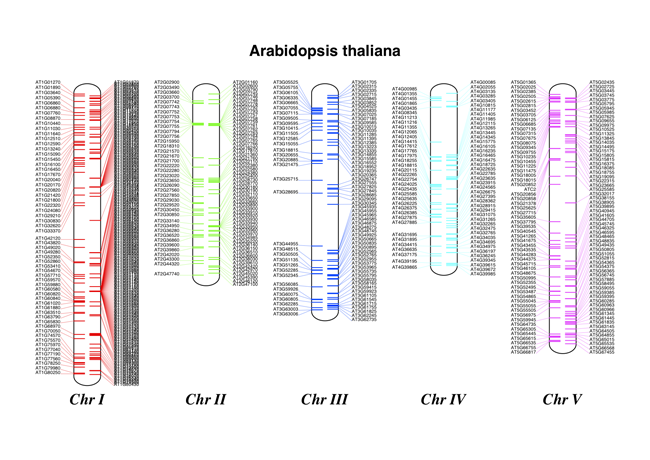
\includegraphics{tRNA_chrom.png}


\chapter{第18章  Cookbook – 用它做一些很酷的事情}
\label{chr18:chapter-cookbook}\label{chr18::doc}\label{chr18:cookbook}
Biopython目前有两个版本的“cookbook”示例——本章(本章包含在教程中许多年,并渐渐成熟),和在Biopython维基上的由用户贡献的集合: \href{http://biopython.org/wiki/Category:Cookbook}{http://biopython.org/wiki/Category:Cookbook} 。

我们在试着鼓励Biopython用户在维基上贡献他们自己的示例。除了能帮助社区之外,分享像这样的示例的一个直接的好处是,你也能从其他Biopython用户和开发者中获得一些关于代码的意见反馈——这或许能帮助你改进自己的Python代码。

长期来说,我们可能最终会将这一章所有的示例都转移到维基上,或者本教程其他的地方。


\section{18.1  操作序列文件}
\label{chr18:id1}
这部分将展示更多使用第 {\hyperref[chr05:chapter-bio-seqio]{\emph{5}}} 章所描述的 \code{Bio.SeqIO} 模块来进行序列输入/输出操作的例子。


\subsection{18.1.1  过滤文件中的序列}
\label{chr18:id2}
通常你会拥有一个包含许多序列的大文件(例如,FASTA基因文件,或者FASTQ或SFF读长文件),和一个包含你所感兴趣的序列的ID列表,而你希望创建一个由这一ID列表里的序列构成的文件。

让我们假设这个ID列表在一个简单的文本文件中,作为每一行的第一个词。这可能是一个表格文件,其第一列是序列ID。尝试下面的代码:
\DUspan{keyword,namespace}{}\DUspan{name,namespace}{}\DUspan{keyword,namespace}{}\DUspan{name}{}\DUspan{name}{}\DUspan{operator}{}\DUspan{literal,string}{}\DUspan{name}{}\DUspan{operator}{}\DUspan{literal,string}{}\DUspan{name}{}\DUspan{operator}{}\DUspan{literal,string}{}\DUspan{name}{}\DUspan{operator}{}\DUspan{name,builtin}{}\DUspan{punctuation}{}\DUspan{name}{}\DUspan{operator}{}\DUspan{name}{}\DUspan{punctuation}{}\DUspan{literal,string}{}\DUspan{literal,string,escape}{}\DUspan{literal,string}{}\DUspan{punctuation}{}\DUspan{operator}{}\DUspan{name}{}\DUspan{punctuation}{}\DUspan{name,builtin,pseudo}{}\DUspan{punctuation}{}\DUspan{literal,number,integer}{}\DUspan{punctuation}{}\DUspan{literal,number,integer}{}\DUspan{punctuation}{}\DUspan{keyword}{}\DUspan{name}{}\DUspan{operator,word}{}\DUspan{name,builtin}{}\DUspan{punctuation}{}\DUspan{name}{}\DUspan{punctuation}{}\DUspan{keyword}{}\DUspan{literal,string}{}\DUspan{literal,string,interpol}{}\DUspan{literal,string}{}\DUspan{literal,string,interpol}{}\DUspan{literal,string}{}\DUspan{operator}{}\DUspan{punctuation}{}\DUspan{name,builtin}{}\DUspan{punctuation}{}\DUspan{name}{}\DUspan{punctuation}{}\DUspan{name}{}\DUspan{punctuation}{}\DUspan{name}{}\DUspan{operator}{}\DUspan{punctuation}{}\DUspan{name}{}\DUspan{keyword}{}\DUspan{name}{}\DUspan{operator,word}{}\DUspan{name}{}\DUspan{operator}{}\DUspan{name}{}\DUspan{punctuation}{}\DUspan{name}{}\DUspan{punctuation}{}\DUspan{literal,string}{}\DUspan{punctuation}{}\DUspan{keyword}{}\DUspan{name}{}\DUspan{operator}{}\DUspan{name}{}\DUspan{operator,word}{}\DUspan{name}{}\DUspan{punctuation}{}\DUspan{name}{}\DUspan{operator}{}\DUspan{name}{}\DUspan{operator}{}\DUspan{name}{}\DUspan{punctuation}{}\DUspan{name}{}\DUspan{punctuation}{}\DUspan{name}{}\DUspan{punctuation}{}\DUspan{literal,string}{}\DUspan{punctuation}{}\DUspan{keyword}{}\DUspan{literal,string}{}\DUspan{literal,string,interpol}{}\DUspan{literal,string}{}\DUspan{literal,string,interpol}{}\DUspan{literal,string}{}\DUspan{literal,string,interpol}{}\DUspan{literal,string}{}\DUspan{operator}{}\DUspan{punctuation}{}\DUspan{name}{}\DUspan{punctuation}{}\DUspan{name}{}\DUspan{punctuation}{}\DUspan{name}{}\DUspan{punctuation}{}\DUspan{keyword}{}\DUspan{name}{}\DUspan{operator}{}\DUspan{name,builtin}{}\DUspan{punctuation}{}\DUspan{name}{}\DUspan{punctuation}{}\DUspan{keyword}{}\DUspan{literal,string}{}\DUspan{literal,string,interpol}{}\DUspan{literal,string}{}\DUspan{literal,string,interpol}{}\DUspan{literal,string}{}\DUspan{operator}{}\DUspan{punctuation}{}\DUspan{name,builtin}{}\DUspan{punctuation}{}\DUspan{name}{}\DUspan{punctuation}{}\DUspan{operator}{}\DUspan{name}{}\DUspan{punctuation}{}\DUspan{name}{}\DUspan{punctuation}{}
\begin{Verbatim}[commandchars=\\\{\}]
\PYG{k+kn}{from} \PYG{n+nn}{Bio} \PYG{k+kn}{import} \PYG{n}{SeqIO}
\PYG{n}{input\PYGZus{}file} \PYG{o}{=} \PYG{l+s}{\PYGZdq{}}\PYG{l+s}{big\PYGZus{}file.sff}\PYG{l+s}{\PYGZdq{}}
\PYG{n}{id\PYGZus{}file} \PYG{o}{=} \PYG{l+s}{\PYGZdq{}}\PYG{l+s}{short\PYGZus{}list.txt}\PYG{l+s}{\PYGZdq{}}
\PYG{n}{output\PYGZus{}file} \PYG{o}{=} \PYG{l+s}{\PYGZdq{}}\PYG{l+s}{short\PYGZus{}list.sff}\PYG{l+s}{\PYGZdq{}}
\PYG{n}{wanted} \PYG{o}{=} \PYG{n+nb}{set}\PYG{p}{(}\PYG{n}{line}\PYG{o}{.}\PYG{n}{rstrip}\PYG{p}{(}\PYG{l+s}{\PYGZdq{}}\PYG{l+s+se}{\PYGZbs{}n}\PYG{l+s}{\PYGZdq{}}\PYG{p}{)}\PYG{o}{.}\PYG{n}{split}\PYG{p}{(}\PYG{n+nb+bp}{None}\PYG{p}{,}\PYG{l+m+mi}{1}\PYG{p}{)}\PYG{p}{[}\PYG{l+m+mi}{0}\PYG{p}{]} \PYG{k}{for} \PYG{n}{line} \PYG{o+ow}{in} \PYG{n+nb}{open}\PYG{p}{(}\PYG{n}{id\PYGZus{}file}\PYG{p}{)}\PYG{p}{)}
\PYG{k}{print} \PYG{l+s}{\PYGZdq{}}\PYG{l+s}{Found }\PYG{l+s+si}{\PYGZpc{}i}\PYG{l+s}{ unique identifiers in }\PYG{l+s+si}{\PYGZpc{}s}\PYG{l+s}{\PYGZdq{}} \PYG{o}{\PYGZpc{}} \PYG{p}{(}\PYG{n+nb}{len}\PYG{p}{(}\PYG{n}{wanted}\PYG{p}{)}\PYG{p}{,} \PYG{n}{id\PYGZus{}file}\PYG{p}{)}
\PYG{n}{records} \PYG{o}{=} \PYG{p}{(}\PYG{n}{r} \PYG{k}{for} \PYG{n}{r} \PYG{o+ow}{in} \PYG{n}{SeqIO}\PYG{o}{.}\PYG{n}{parse}\PYG{p}{(}\PYG{n}{input\PYGZus{}file}\PYG{p}{,} \PYG{l+s}{\PYGZdq{}}\PYG{l+s}{sff}\PYG{l+s}{\PYGZdq{}}\PYG{p}{)} \PYG{k}{if} \PYG{n}{r}\PYG{o}{.}\PYG{n}{id} \PYG{o+ow}{in} \PYG{n}{wanted}\PYG{p}{)}
\PYG{n}{count} \PYG{o}{=} \PYG{n}{SeqIO}\PYG{o}{.}\PYG{n}{write}\PYG{p}{(}\PYG{n}{records}\PYG{p}{,} \PYG{n}{output\PYGZus{}file}\PYG{p}{,} \PYG{l+s}{\PYGZdq{}}\PYG{l+s}{sff}\PYG{l+s}{\PYGZdq{}}\PYG{p}{)}
\PYG{k}{print} \PYG{l+s}{\PYGZdq{}}\PYG{l+s}{Saved }\PYG{l+s+si}{\PYGZpc{}i}\PYG{l+s}{ records from }\PYG{l+s+si}{\PYGZpc{}s}\PYG{l+s}{ to }\PYG{l+s+si}{\PYGZpc{}s}\PYG{l+s}{\PYGZdq{}} \PYG{o}{\PYGZpc{}} \PYG{p}{(}\PYG{n}{count}\PYG{p}{,} \PYG{n}{input\PYGZus{}file}\PYG{p}{,} \PYG{n}{output\PYGZus{}file}\PYG{p}{)}
\PYG{k}{if} \PYG{n}{count} \PYG{o}{\PYGZlt{}} \PYG{n+nb}{len}\PYG{p}{(}\PYG{n}{wanted}\PYG{p}{)}\PYG{p}{:}
    \PYG{k}{print} \PYG{l+s}{\PYGZdq{}}\PYG{l+s}{Warning }\PYG{l+s+si}{\PYGZpc{}i}\PYG{l+s}{ IDs not found in }\PYG{l+s+si}{\PYGZpc{}s}\PYG{l+s}{\PYGZdq{}} \PYG{o}{\PYGZpc{}} \PYG{p}{(}\PYG{n+nb}{len}\PYG{p}{(}\PYG{n}{wanted}\PYG{p}{)}\PYG{o}{\PYGZhy{}}\PYG{n}{count}\PYG{p}{,} \PYG{n}{input\PYGZus{}file}\PYG{p}{)}
\end{Verbatim}

注意,我们使用Python的 \code{set} 类型而不是 \code{list},这会使得检测成员关系更快。


\subsection{18.1.2  生成随机基因组}
\label{chr18:id3}
假设你在检视一个基因组序列,寻找一些序列特征——或许是极端局部GC含量偏差,或者可能的限制性酶切位点。一旦你使你的Python代码在真实的基因组上运行后,尝试在相同的随机化版本基因组上运行,并进行统计分析或许是明智的选择(毕竟,任何你发现的“特性”都可能只是偶然事件)。

在这一讨论中,我们将使用来自 \emph{Yersinia pestis biovar Microtus} 的pPCP1质粒的GenBank文件。该文件包含在Biopython单元测试的GenBank文件夹中,或者你可以从我们的网站上得到, \href{http://biopython.org/SRC/biopython/Tests/GenBank/NC\_005816.gb}{NC\_005816.gb}. 该文件仅有一个记录,所以我们能用 \code{Bio.SeqIO.read()} 函数把它当做 \code{SeqRecord} 读入:
\DUspan{operator}{}\DUspan{keyword,namespace}{}\DUspan{name,namespace}{}\DUspan{keyword,namespace}{}\DUspan{name}{}\DUspan{operator}{}\DUspan{name}{}\DUspan{operator}{}\DUspan{name}{}\DUspan{operator}{}\DUspan{name}{}\DUspan{punctuation}{}\DUspan{literal,string}{}\DUspan{punctuation}{}\DUspan{literal,string}{}\DUspan{punctuation}{}
\begin{Verbatim}[commandchars=\\\{\}]
\PYG{g+gp}{\PYGZgt{}\PYGZgt{}\PYGZgt{} }\PYG{k+kn}{from} \PYG{n+nn}{Bio} \PYG{k+kn}{import} \PYG{n}{SeqIO}
\PYG{g+gp}{\PYGZgt{}\PYGZgt{}\PYGZgt{} }\PYG{n}{original\PYGZus{}rec} \PYG{o}{=} \PYG{n}{SeqIO}\PYG{o}{.}\PYG{n}{read}\PYG{p}{(}\PYG{l+s}{\PYGZdq{}}\PYG{l+s}{NC\PYGZus{}005816.gb}\PYG{l+s}{\PYGZdq{}}\PYG{p}{,}\PYG{l+s}{\PYGZdq{}}\PYG{l+s}{genbank}\PYG{l+s}{\PYGZdq{}}\PYG{p}{)}
\end{Verbatim}

那么,我们怎么生成一个原始序列重排后的版本能?我会使用Python内置的 \code{random} 模块来做这个,特别是 \code{random.shuffle} 函数——但是这个只作用于Python列表。我们的序列是一个 \code{Seq} 对象,所以为了重排它,我们需要将它转换为一个列表:
\DUspan{operator}{}\DUspan{keyword,namespace}{}\DUspan{name,namespace}{}\DUspan{operator}{}\DUspan{name}{}\DUspan{operator}{}\DUspan{name,builtin}{}\DUspan{punctuation}{}\DUspan{name}{}\DUspan{operator}{}\DUspan{name}{}\DUspan{punctuation}{}\DUspan{operator}{}\DUspan{name}{}\DUspan{operator}{}\DUspan{name}{}\DUspan{punctuation}{}\DUspan{name}{}\DUspan{punctuation}{}\DUspan{comment}{}
\begin{Verbatim}[commandchars=\\\{\}]
\PYG{g+gp}{\PYGZgt{}\PYGZgt{}\PYGZgt{} }\PYG{k+kn}{import} \PYG{n+nn}{random}
\PYG{g+gp}{\PYGZgt{}\PYGZgt{}\PYGZgt{} }\PYG{n}{nuc\PYGZus{}list} \PYG{o}{=} \PYG{n+nb}{list}\PYG{p}{(}\PYG{n}{original\PYGZus{}rec}\PYG{o}{.}\PYG{n}{seq}\PYG{p}{)}
\PYG{g+gp}{\PYGZgt{}\PYGZgt{}\PYGZgt{} }\PYG{n}{random}\PYG{o}{.}\PYG{n}{shuffle}\PYG{p}{(}\PYG{n}{nuc\PYGZus{}list}\PYG{p}{)} \PYG{c}{\PYGZsh{}acts in situ!}
\end{Verbatim}

现在,为了使用 \code{Bio.SeqIO} 输出重排的序列,我们需要使用重排后的列表重新创建包含一个新的 \code{SeqRecord} 包含随即化后的 \code{Seq} 。要实现这个,我们需要将核苷酸(单字母字符串)列表转换为长字符串——在Python中,一般使用字符串对象的join方法来实现它。
\DUspan{operator}{}\DUspan{keyword,namespace}{}\DUspan{name,namespace}{}\DUspan{keyword,namespace}{}\DUspan{name}{}\DUspan{operator}{}\DUspan{keyword,namespace}{}\DUspan{name,namespace}{}\DUspan{keyword,namespace}{}\DUspan{name}{}\DUspan{operator}{}\DUspan{name}{}\DUspan{operator}{}\DUspan{name}{}\DUspan{punctuation}{}\DUspan{name}{}\DUspan{punctuation}{}\DUspan{literal,string}{}\DUspan{operator}{}\DUspan{name}{}\DUspan{punctuation}{}\DUspan{name}{}\DUspan{punctuation}{}\DUspan{name}{}\DUspan{operator}{}\DUspan{name}{}\DUspan{operator}{}\DUspan{name}{}\DUspan{punctuation}{}\DUspan{operator}{}\DUspan{name,builtin}{}\DUspan{operator}{}\DUspan{literal,string}{}\DUspan{punctuation}{}\DUspan{name}{}\DUspan{operator}{}\DUspan{literal,string}{}\DUspan{literal,string,interpol}{}\DUspan{literal,string}{}\DUspan{operator}{}\DUspan{name}{}\DUspan{operator}{}\DUspan{name}{}\DUspan{punctuation}{}
\begin{Verbatim}[commandchars=\\\{\}]
\PYG{g+gp}{\PYGZgt{}\PYGZgt{}\PYGZgt{} }\PYG{k+kn}{from} \PYG{n+nn}{Bio.Seq} \PYG{k+kn}{import} \PYG{n}{Seq}
\PYG{g+gp}{\PYGZgt{}\PYGZgt{}\PYGZgt{} }\PYG{k+kn}{from} \PYG{n+nn}{Bio.SeqRecord} \PYG{k+kn}{import} \PYG{n}{SeqRecord}
\PYG{g+gp}{\PYGZgt{}\PYGZgt{}\PYGZgt{} }\PYG{n}{shuffled\PYGZus{}rec} \PYG{o}{=} \PYG{n}{SeqRecord}\PYG{p}{(}\PYG{n}{Seq}\PYG{p}{(}\PYG{l+s}{\PYGZdq{}}\PYG{l+s}{\PYGZdq{}}\PYG{o}{.}\PYG{n}{join}\PYG{p}{(}\PYG{n}{nuc\PYGZus{}list}\PYG{p}{)}\PYG{p}{,} \PYG{n}{original\PYGZus{}rec}\PYG{o}{.}\PYG{n}{seq}\PYG{o}{.}\PYG{n}{alphabet}\PYG{p}{)}\PYG{p}{,}
\PYG{g+gp}{... }                         \PYG{n+nb}{id}\PYG{o}{=}\PYG{l+s}{\PYGZdq{}}\PYG{l+s}{Shuffled}\PYG{l+s}{\PYGZdq{}}\PYG{p}{,} \PYG{n}{description}\PYG{o}{=}\PYG{l+s}{\PYGZdq{}}\PYG{l+s}{Based on }\PYG{l+s+si}{\PYGZpc{}s}\PYG{l+s}{\PYGZdq{}} \PYG{o}{\PYGZpc{}} \PYG{n}{original\PYGZus{}rec}\PYG{o}{.}\PYG{n}{id}\PYG{p}{)}
\end{Verbatim}

让我们将所有这些片段放到一起来组成一个完整的Python脚本,这个脚本将生成一个FASTA序列文件,其包含30个原始序列的随机重排版本。

第一个版本只是使用一个大的for循环,并一个一个的输出记录(使用章节 {\hyperref[chr05:sec-bio-seqio-and-stringio]{\emph{5.5.4}}} 描述的{}`{}`SeqRecord{}`{}` 的格式化方法):
\DUspan{keyword,namespace}{}\DUspan{name,namespace}{}\DUspan{keyword,namespace}{}\DUspan{name,namespace}{}\DUspan{keyword,namespace}{}\DUspan{name}{}\DUspan{keyword,namespace}{}\DUspan{name,namespace}{}\DUspan{keyword,namespace}{}\DUspan{name}{}\DUspan{keyword,namespace}{}\DUspan{name,namespace}{}\DUspan{keyword,namespace}{}\DUspan{name}{}\DUspan{name}{}\DUspan{operator}{}\DUspan{name}{}\DUspan{operator}{}\DUspan{name}{}\DUspan{punctuation}{}\DUspan{literal,string}{}\DUspan{punctuation}{}\DUspan{literal,string}{}\DUspan{punctuation}{}\DUspan{name}{}\DUspan{operator}{}\DUspan{name,builtin}{}\DUspan{punctuation}{}\DUspan{literal,string}{}\DUspan{punctuation}{}\DUspan{literal,string}{}\DUspan{punctuation}{}\DUspan{keyword}{}\DUspan{name}{}\DUspan{operator,word}{}\DUspan{name,builtin}{}\DUspan{punctuation}{}\DUspan{literal,number,integer}{}\DUspan{punctuation}{}\DUspan{name}{}\DUspan{operator}{}\DUspan{name,builtin}{}\DUspan{punctuation}{}\DUspan{name}{}\DUspan{operator}{}\DUspan{name}{}\DUspan{punctuation}{}\DUspan{name}{}\DUspan{operator}{}\DUspan{name}{}\DUspan{punctuation}{}\DUspan{name}{}\DUspan{punctuation}{}\DUspan{name}{}\DUspan{operator}{}\DUspan{name}{}\DUspan{punctuation}{}\DUspan{name}{}\DUspan{punctuation}{}\DUspan{literal,string}{}\DUspan{operator}{}\DUspan{name}{}\DUspan{punctuation}{}\DUspan{name}{}\DUspan{punctuation}{}\DUspan{name}{}\DUspan{operator}{}\DUspan{name}{}\DUspan{operator}{}\DUspan{name}{}\DUspan{punctuation}{}\DUspan{name,builtin}{}\DUspan{operator}{}\DUspan{literal,string}{}\DUspan{literal,string,interpol}{}\DUspan{literal,string}{}\DUspan{operator}{}\DUspan{punctuation}{}\DUspan{name}{}\DUspan{operator}{}\DUspan{literal,number,integer}{}\DUspan{punctuation}{}\DUspan{name}{}\DUspan{operator}{}\DUspan{literal,string}{}\DUspan{literal,string,interpol}{}\DUspan{literal,string}{}\DUspan{operator}{}\DUspan{name}{}\DUspan{operator}{}\DUspan{name}{}\DUspan{punctuation}{}\DUspan{name}{}\DUspan{operator}{}\DUspan{name}{}\DUspan{punctuation}{}\DUspan{name}{}\DUspan{operator}{}\DUspan{name}{}\DUspan{punctuation}{}\DUspan{literal,string}{}\DUspan{punctuation}{}\DUspan{name}{}\DUspan{operator}{}\DUspan{name}{}\DUspan{punctuation}{}
\begin{Verbatim}[commandchars=\\\{\}]
\PYG{k+kn}{import} \PYG{n+nn}{random}
\PYG{k+kn}{from} \PYG{n+nn}{Bio.Seq} \PYG{k+kn}{import} \PYG{n}{Seq}
\PYG{k+kn}{from} \PYG{n+nn}{Bio.SeqRecord} \PYG{k+kn}{import} \PYG{n}{SeqRecord}
\PYG{k+kn}{from} \PYG{n+nn}{Bio} \PYG{k+kn}{import} \PYG{n}{SeqIO}

\PYG{n}{original\PYGZus{}rec} \PYG{o}{=} \PYG{n}{SeqIO}\PYG{o}{.}\PYG{n}{read}\PYG{p}{(}\PYG{l+s}{\PYGZdq{}}\PYG{l+s}{NC\PYGZus{}005816.gb}\PYG{l+s}{\PYGZdq{}}\PYG{p}{,}\PYG{l+s}{\PYGZdq{}}\PYG{l+s}{genbank}\PYG{l+s}{\PYGZdq{}}\PYG{p}{)}

\PYG{n}{handle} \PYG{o}{=} \PYG{n+nb}{open}\PYG{p}{(}\PYG{l+s}{\PYGZdq{}}\PYG{l+s}{shuffled.fasta}\PYG{l+s}{\PYGZdq{}}\PYG{p}{,} \PYG{l+s}{\PYGZdq{}}\PYG{l+s}{w}\PYG{l+s}{\PYGZdq{}}\PYG{p}{)}
\PYG{k}{for} \PYG{n}{i} \PYG{o+ow}{in} \PYG{n+nb}{range}\PYG{p}{(}\PYG{l+m+mi}{30}\PYG{p}{)}\PYG{p}{:}
    \PYG{n}{nuc\PYGZus{}list} \PYG{o}{=} \PYG{n+nb}{list}\PYG{p}{(}\PYG{n}{original\PYGZus{}rec}\PYG{o}{.}\PYG{n}{seq}\PYG{p}{)}
    \PYG{n}{random}\PYG{o}{.}\PYG{n}{shuffle}\PYG{p}{(}\PYG{n}{nuc\PYGZus{}list}\PYG{p}{)}
    \PYG{n}{shuffled\PYGZus{}rec} \PYG{o}{=} \PYG{n}{SeqRecord}\PYG{p}{(}\PYG{n}{Seq}\PYG{p}{(}\PYG{l+s}{\PYGZdq{}}\PYG{l+s}{\PYGZdq{}}\PYG{o}{.}\PYG{n}{join}\PYG{p}{(}\PYG{n}{nuc\PYGZus{}list}\PYG{p}{)}\PYG{p}{,} \PYG{n}{original\PYGZus{}rec}\PYG{o}{.}\PYG{n}{seq}\PYG{o}{.}\PYG{n}{alphabet}\PYG{p}{)}\PYG{p}{,} \PYGZbs{}
                             \PYG{n+nb}{id}\PYG{o}{=}\PYG{l+s}{\PYGZdq{}}\PYG{l+s}{Shuffled}\PYG{l+s+si}{\PYGZpc{}i}\PYG{l+s}{\PYGZdq{}} \PYG{o}{\PYGZpc{}} \PYG{p}{(}\PYG{n}{i}\PYG{o}{+}\PYG{l+m+mi}{1}\PYG{p}{)}\PYG{p}{,} \PYGZbs{}
                             \PYG{n}{description}\PYG{o}{=}\PYG{l+s}{\PYGZdq{}}\PYG{l+s}{Based on }\PYG{l+s+si}{\PYGZpc{}s}\PYG{l+s}{\PYGZdq{}} \PYG{o}{\PYGZpc{}} \PYG{n}{original\PYGZus{}rec}\PYG{o}{.}\PYG{n}{id}\PYG{p}{)}
    \PYG{n}{handle}\PYG{o}{.}\PYG{n}{write}\PYG{p}{(}\PYG{n}{shuffled\PYGZus{}rec}\PYG{o}{.}\PYG{n}{format}\PYG{p}{(}\PYG{l+s}{\PYGZdq{}}\PYG{l+s}{fasta}\PYG{l+s}{\PYGZdq{}}\PYG{p}{)}\PYG{p}{)}
\PYG{n}{handle}\PYG{o}{.}\PYG{n}{close}\PYG{p}{(}\PYG{p}{)}
\end{Verbatim}

我个人更喜欢下面的版本(不使用for循环),而使用一个函数来重排记录以及一个生成表达式:
\DUspan{keyword,namespace}{}\DUspan{name,namespace}{}\DUspan{keyword,namespace}{}\DUspan{name,namespace}{}\DUspan{keyword,namespace}{}\DUspan{name}{}\DUspan{keyword,namespace}{}\DUspan{name,namespace}{}\DUspan{keyword,namespace}{}\DUspan{name}{}\DUspan{keyword,namespace}{}\DUspan{name,namespace}{}\DUspan{keyword,namespace}{}\DUspan{name}{}\DUspan{keyword}{}\DUspan{name,function}{}\DUspan{punctuation}{}\DUspan{name}{}\DUspan{punctuation}{}\DUspan{name}{}\DUspan{punctuation}{}\DUspan{name}{}\DUspan{operator}{}\DUspan{name,builtin}{}\DUspan{punctuation}{}\DUspan{name}{}\DUspan{operator}{}\DUspan{name}{}\DUspan{punctuation}{}\DUspan{name}{}\DUspan{operator}{}\DUspan{name}{}\DUspan{punctuation}{}\DUspan{name}{}\DUspan{punctuation}{}\DUspan{keyword}{}\DUspan{name}{}\DUspan{punctuation}{}\DUspan{name}{}\DUspan{punctuation}{}\DUspan{literal,string}{}\DUspan{operator}{}\DUspan{name}{}\DUspan{punctuation}{}\DUspan{name}{}\DUspan{punctuation}{}\DUspan{name}{}\DUspan{operator}{}\DUspan{name}{}\DUspan{operator}{}\DUspan{name}{}\DUspan{punctuation}{}\DUspan{name,builtin}{}\DUspan{operator}{}\DUspan{name}{}\DUspan{punctuation}{}\DUspan{name}{}\DUspan{operator}{}\DUspan{literal,string}{}\DUspan{literal,string,interpol}{}\DUspan{literal,string}{}\DUspan{operator}{}\DUspan{name}{}\DUspan{operator}{}\DUspan{name}{}\DUspan{punctuation}{}\DUspan{name}{}\DUspan{operator}{}\DUspan{name}{}\DUspan{operator}{}\DUspan{name}{}\DUspan{punctuation}{}\DUspan{literal,string}{}\DUspan{punctuation}{}\DUspan{literal,string}{}\DUspan{punctuation}{}\DUspan{name}{}\DUspan{operator}{}\DUspan{punctuation}{}\DUspan{name}{}\DUspan{punctuation}{}\DUspan{name}{}\DUspan{punctuation}{}\DUspan{literal,string}{}\DUspan{literal,string,interpol}{}\DUspan{literal,string}{}\DUspan{operator}{}\DUspan{punctuation}{}\DUspan{name}{}\DUspan{operator}{}\DUspan{literal,number,integer}{}\DUspan{punctuation}{}\DUspan{keyword}{}\DUspan{name}{}\DUspan{operator,word}{}\DUspan{name,builtin}{}\DUspan{punctuation}{}\DUspan{literal,number,integer}{}\DUspan{punctuation}{}\DUspan{name}{}\DUspan{operator}{}\DUspan{name,builtin}{}\DUspan{punctuation}{}\DUspan{literal,string}{}\DUspan{punctuation}{}\DUspan{literal,string}{}\DUspan{punctuation}{}\DUspan{name}{}\DUspan{operator}{}\DUspan{name}{}\DUspan{punctuation}{}\DUspan{name}{}\DUspan{punctuation}{}\DUspan{name}{}\DUspan{punctuation}{}\DUspan{literal,string}{}\DUspan{punctuation}{}\DUspan{name}{}\DUspan{operator}{}\DUspan{name}{}\DUspan{punctuation}{}
\begin{Verbatim}[commandchars=\\\{\}]
\PYG{k+kn}{import} \PYG{n+nn}{random}
\PYG{k+kn}{from} \PYG{n+nn}{Bio.Seq} \PYG{k+kn}{import} \PYG{n}{Seq}
\PYG{k+kn}{from} \PYG{n+nn}{Bio.SeqRecord} \PYG{k+kn}{import} \PYG{n}{SeqRecord}
\PYG{k+kn}{from} \PYG{n+nn}{Bio} \PYG{k+kn}{import} \PYG{n}{SeqIO}

\PYG{k}{def} \PYG{n+nf}{make\PYGZus{}shuffle\PYGZus{}record}\PYG{p}{(}\PYG{n}{record}\PYG{p}{,} \PYG{n}{new\PYGZus{}id}\PYG{p}{)}\PYG{p}{:}
    \PYG{n}{nuc\PYGZus{}list} \PYG{o}{=} \PYG{n+nb}{list}\PYG{p}{(}\PYG{n}{record}\PYG{o}{.}\PYG{n}{seq}\PYG{p}{)}
    \PYG{n}{random}\PYG{o}{.}\PYG{n}{shuffle}\PYG{p}{(}\PYG{n}{nuc\PYGZus{}list}\PYG{p}{)}
    \PYG{k}{return} \PYG{n}{SeqRecord}\PYG{p}{(}\PYG{n}{Seq}\PYG{p}{(}\PYG{l+s}{\PYGZdq{}}\PYG{l+s}{\PYGZdq{}}\PYG{o}{.}\PYG{n}{join}\PYG{p}{(}\PYG{n}{nuc\PYGZus{}list}\PYG{p}{)}\PYG{p}{,} \PYG{n}{record}\PYG{o}{.}\PYG{n}{seq}\PYG{o}{.}\PYG{n}{alphabet}\PYG{p}{)}\PYG{p}{,} \PYGZbs{}
           \PYG{n+nb}{id}\PYG{o}{=}\PYG{n}{new\PYGZus{}id}\PYG{p}{,} \PYG{n}{description}\PYG{o}{=}\PYG{l+s}{\PYGZdq{}}\PYG{l+s}{Based on }\PYG{l+s+si}{\PYGZpc{}s}\PYG{l+s}{\PYGZdq{}} \PYG{o}{\PYGZpc{}} \PYG{n}{original\PYGZus{}rec}\PYG{o}{.}\PYG{n}{id}\PYG{p}{)}

\PYG{n}{original\PYGZus{}rec} \PYG{o}{=} \PYG{n}{SeqIO}\PYG{o}{.}\PYG{n}{read}\PYG{p}{(}\PYG{l+s}{\PYGZdq{}}\PYG{l+s}{NC\PYGZus{}005816.gb}\PYG{l+s}{\PYGZdq{}}\PYG{p}{,}\PYG{l+s}{\PYGZdq{}}\PYG{l+s}{genbank}\PYG{l+s}{\PYGZdq{}}\PYG{p}{)}
\PYG{n}{shuffled\PYGZus{}recs} \PYG{o}{=} \PYG{p}{(}\PYG{n}{make\PYGZus{}shuffle\PYGZus{}record}\PYG{p}{(}\PYG{n}{original\PYGZus{}rec}\PYG{p}{,} \PYG{l+s}{\PYGZdq{}}\PYG{l+s}{Shuffled}\PYG{l+s+si}{\PYGZpc{}i}\PYG{l+s}{\PYGZdq{}} \PYG{o}{\PYGZpc{}} \PYG{p}{(}\PYG{n}{i}\PYG{o}{+}\PYG{l+m+mi}{1}\PYG{p}{)}\PYG{p}{)} \PYGZbs{}
                 \PYG{k}{for} \PYG{n}{i} \PYG{o+ow}{in} \PYG{n+nb}{range}\PYG{p}{(}\PYG{l+m+mi}{30}\PYG{p}{)}\PYG{p}{)}
\PYG{n}{handle} \PYG{o}{=} \PYG{n+nb}{open}\PYG{p}{(}\PYG{l+s}{\PYGZdq{}}\PYG{l+s}{shuffled.fasta}\PYG{l+s}{\PYGZdq{}}\PYG{p}{,} \PYG{l+s}{\PYGZdq{}}\PYG{l+s}{w}\PYG{l+s}{\PYGZdq{}}\PYG{p}{)}
\PYG{n}{SeqIO}\PYG{o}{.}\PYG{n}{write}\PYG{p}{(}\PYG{n}{shuffled\PYGZus{}recs}\PYG{p}{,} \PYG{n}{handle}\PYG{p}{,} \PYG{l+s}{\PYGZdq{}}\PYG{l+s}{fasta}\PYG{l+s}{\PYGZdq{}}\PYG{p}{)}
\PYG{n}{handle}\PYG{o}{.}\PYG{n}{close}\PYG{p}{(}\PYG{p}{)}
\end{Verbatim}


\subsection{18.1.3  翻译CDS条目为FASTA文件}
\label{chr18:cdsfasta}\label{chr18:sec-seqio-translate}
假设你有一个包含某个物种的CDS条目作为输入文件,你想生成一个由它们的蛋白序列组成的FASTA文件。也就是,从原始文件中取出每一个核苷酸序列,并翻译它。回到章节 {\hyperref[chr03:sec-translation]{\emph{3.9}}} 我们了解了怎么使用 \code{Seq} 对象的 \code{translate} 方法,和可选的 \code{cds} 参数来使得不同的起始密码子能正确翻译。

就像章节 {\hyperref[chr05:sec-seqio-reverse-complement]{\emph{5.5.3}}} 中反向互补的例子中展示的那样,我们可以用 \code{Bio.SeqIO} 将与翻译步骤结合起来。对于每一个核苷酸 \code{SeqRecord} ,我们需要创建一个蛋白的 \code{SeqRecord} —— 并对它命名。

你能编写自己的函数来做这个事情,为你的序列选择合适的蛋白标识和恰当的密码表。在本例中,我们仅使用默认的密码表,并给序列ID加一个前缀。
\DUspan{keyword,namespace}{}\DUspan{name,namespace}{}\DUspan{keyword,namespace}{}\DUspan{name}{}\DUspan{keyword}{}\DUspan{name,function}{}\DUspan{punctuation}{}\DUspan{name}{}\DUspan{punctuation}{}\DUspan{literal,string,doc}{}\DUspan{keyword}{}\DUspan{name}{}\DUspan{punctuation}{}\DUspan{name}{}\DUspan{operator}{}\DUspan{name}{}\DUspan{operator}{}\DUspan{name}{}\DUspan{operator}{}\DUspan{name}{}\DUspan{punctuation}{}\DUspan{name}{}\DUspan{operator}{}\DUspan{name,builtin,pseudo}{}\DUspan{punctuation}{}\DUspan{name,builtin}{}\DUspan{operator}{}\DUspan{literal,string}{}\DUspan{operator}{}\DUspan{name}{}\DUspan{operator}{}\DUspan{name}{}\DUspan{punctuation}{}\DUspan{name}{}\DUspan{operator}{}\DUspan{literal,string}{}\DUspan{punctuation}{}
\begin{Verbatim}[commandchars=\\\{\}]
\PYG{k+kn}{from} \PYG{n+nn}{Bio.SeqRecord} \PYG{k+kn}{import} \PYG{n}{SeqRecord}
\PYG{k}{def} \PYG{n+nf}{make\PYGZus{}protein\PYGZus{}record}\PYG{p}{(}\PYG{n}{nuc\PYGZus{}record}\PYG{p}{)}\PYG{p}{:}
    \PYG{l+s+sd}{\PYGZdq{}\PYGZdq{}\PYGZdq{}Returns a new SeqRecord with the translated sequence (default table).\PYGZdq{}\PYGZdq{}\PYGZdq{}}
    \PYG{k}{return} \PYG{n}{SeqRecord}\PYG{p}{(}\PYG{n}{seq} \PYG{o}{=} \PYG{n}{nuc\PYGZus{}record}\PYG{o}{.}\PYG{n}{seq}\PYG{o}{.}\PYG{n}{translate}\PYG{p}{(}\PYG{n}{cds}\PYG{o}{=}\PYG{n+nb+bp}{True}\PYG{p}{)}\PYG{p}{,} \PYGZbs{}
                     \PYG{n+nb}{id} \PYG{o}{=} \PYG{l+s}{\PYGZdq{}}\PYG{l+s}{trans\PYGZus{}}\PYG{l+s}{\PYGZdq{}} \PYG{o}{+} \PYG{n}{nuc\PYGZus{}record}\PYG{o}{.}\PYG{n}{id}\PYG{p}{,} \PYGZbs{}
                     \PYG{n}{description} \PYG{o}{=} \PYG{l+s}{\PYGZdq{}}\PYG{l+s}{translation of CDS, using default table}\PYG{l+s}{\PYGZdq{}}\PYG{p}{)}
\end{Verbatim}

我们能用这个函数将核苷酸记录转换为蛋白记录,作为输出。一个优雅且内存高效的方式是使用生成表达式(generator expression):
\DUspan{keyword,namespace}{}\DUspan{name,namespace}{}\DUspan{keyword,namespace}{}\DUspan{name}{}\DUspan{name}{}\DUspan{operator}{}\DUspan{punctuation}{}\DUspan{name}{}\DUspan{punctuation}{}\DUspan{name}{}\DUspan{punctuation}{}\DUspan{keyword}{}\DUspan{name}{}\DUspan{operator,word}{}\DUspan{name}{}\DUspan{operator}{}\DUspan{name}{}\DUspan{punctuation}{}\DUspan{literal,string}{}\DUspan{punctuation}{}\DUspan{literal,string}{}\DUspan{punctuation}{}\DUspan{name}{}\DUspan{operator}{}\DUspan{name}{}\DUspan{punctuation}{}\DUspan{name}{}\DUspan{punctuation}{}\DUspan{literal,string}{}\DUspan{punctuation}{}\DUspan{literal,string}{}\DUspan{punctuation}{}
\begin{Verbatim}[commandchars=\\\{\}]
\PYG{k+kn}{from} \PYG{n+nn}{Bio} \PYG{k+kn}{import} \PYG{n}{SeqIO}
\PYG{n}{proteins} \PYG{o}{=} \PYG{p}{(}\PYG{n}{make\PYGZus{}protein\PYGZus{}record}\PYG{p}{(}\PYG{n}{nuc\PYGZus{}rec}\PYG{p}{)} \PYG{k}{for} \PYG{n}{nuc\PYGZus{}rec} \PYG{o+ow}{in} \PYGZbs{}
            \PYG{n}{SeqIO}\PYG{o}{.}\PYG{n}{parse}\PYG{p}{(}\PYG{l+s}{\PYGZdq{}}\PYG{l+s}{coding\PYGZus{}sequences.fasta}\PYG{l+s}{\PYGZdq{}}\PYG{p}{,} \PYG{l+s}{\PYGZdq{}}\PYG{l+s}{fasta}\PYG{l+s}{\PYGZdq{}}\PYG{p}{)}\PYG{p}{)}
\PYG{n}{SeqIO}\PYG{o}{.}\PYG{n}{write}\PYG{p}{(}\PYG{n}{proteins}\PYG{p}{,} \PYG{l+s}{\PYGZdq{}}\PYG{l+s}{translations.fasta}\PYG{l+s}{\PYGZdq{}}\PYG{p}{,} \PYG{l+s}{\PYGZdq{}}\PYG{l+s}{fasta}\PYG{l+s}{\PYGZdq{}}\PYG{p}{)}
\end{Verbatim}

以上代码适用于完整编码序列的FASTA文件。如果你使用部分编码序列,你可能希望在以上的例子中使用 \code{nuc\_record.seq.translate(to\_stop=True)} ,这会告诉Biopython不检查起始密码的有效性,等等。


\subsection{18.1.4  将FASTA文件中的序列变为大写}
\label{chr18:fasta}
通常你会从合作者那里得到FASTA文件的数据,有时候这些序列可能是大小写混合的。在某些情况下,这些可能是有意为之的(例如,小写的作为低质量的区域),但通常大小写并不重要。你可能希望编辑这个文件以使所有的序列都变得一致(如,都为大写),你可以使用 \code{SeqRecord} 对象的 \code{upper()} 方法轻易的实现(Biopython 1.55中引入):
\DUspan{keyword,namespace}{}\DUspan{name,namespace}{}\DUspan{keyword,namespace}{}\DUspan{name}{}\DUspan{name}{}\DUspan{operator}{}\DUspan{punctuation}{}\DUspan{name}{}\DUspan{operator}{}\DUspan{name}{}\DUspan{punctuation}{}\DUspan{keyword}{}\DUspan{name}{}\DUspan{operator,word}{}\DUspan{name}{}\DUspan{operator}{}\DUspan{name}{}\DUspan{punctuation}{}\DUspan{literal,string}{}\DUspan{punctuation}{}\DUspan{literal,string}{}\DUspan{punctuation}{}\DUspan{name}{}\DUspan{operator}{}\DUspan{name}{}\DUspan{operator}{}\DUspan{name}{}\DUspan{punctuation}{}\DUspan{name}{}\DUspan{punctuation}{}\DUspan{literal,string}{}\DUspan{punctuation}{}\DUspan{literal,string}{}\DUspan{punctuation}{}\DUspan{keyword}{}\DUspan{literal,string}{}\DUspan{literal,string,interpol}{}\DUspan{literal,string}{}\DUspan{operator}{}\DUspan{name}{}
\begin{Verbatim}[commandchars=\\\{\}]
\PYG{k+kn}{from} \PYG{n+nn}{Bio} \PYG{k+kn}{import} \PYG{n}{SeqIO}
\PYG{n}{records} \PYG{o}{=} \PYG{p}{(}\PYG{n}{rec}\PYG{o}{.}\PYG{n}{upper}\PYG{p}{(}\PYG{p}{)} \PYG{k}{for} \PYG{n}{rec} \PYG{o+ow}{in} \PYG{n}{SeqIO}\PYG{o}{.}\PYG{n}{parse}\PYG{p}{(}\PYG{l+s}{\PYGZdq{}}\PYG{l+s}{mixed.fas}\PYG{l+s}{\PYGZdq{}}\PYG{p}{,} \PYG{l+s}{\PYGZdq{}}\PYG{l+s}{fasta}\PYG{l+s}{\PYGZdq{}}\PYG{p}{)}\PYG{p}{)}
\PYG{n}{count} \PYG{o}{=} \PYG{n}{SeqIO}\PYG{o}{.}\PYG{n}{write}\PYG{p}{(}\PYG{n}{records}\PYG{p}{,} \PYG{l+s}{\PYGZdq{}}\PYG{l+s}{upper.fas}\PYG{l+s}{\PYGZdq{}}\PYG{p}{,} \PYG{l+s}{\PYGZdq{}}\PYG{l+s}{fasta}\PYG{l+s}{\PYGZdq{}}\PYG{p}{)}
\PYG{k}{print} \PYG{l+s}{\PYGZdq{}}\PYG{l+s}{Converted }\PYG{l+s+si}{\PYGZpc{}i}\PYG{l+s}{ records to upper case}\PYG{l+s}{\PYGZdq{}} \PYG{o}{\PYGZpc{}} \PYG{n}{count}
\end{Verbatim}

这是怎么工作的呢?第一行只是导入 \code{Bio.SeqIO} 模块。第二行是最有趣的——这是一个Python生成器表达式,它提供 \code{mixed.fas} 里每个记录的大写版本。第三行中,我们把这个生成器表达式传给 \code{Bio.SeqIO.write()} 函数,它会把大写的序列写出到 \code{upper.fas} 输出文件。

我们使用生成器(而不是一个列表或列表解析式)的原因是,前一方式每次仅有一个记录保存在内存中。当你在处理包含成千上万的条目的文件时,这可能非常重要。


\subsection{18.1.5  对序列文件排序}
\label{chr18:id4}\label{chr18:sec-seqio-sort}
假设你想对一个序列文件按序列长度排序(例如,一个序列拼接的重叠群(contig)集合),而你工作的文件格式可能是像FASTA或FASTQ这样 \code{Bio.SeqIO} 能读写(和索引)的格式。

如果文件足够小,你能将它都一次读入内存为一个 \code{SeqRecord} 对象列表,对列表进行排序,并保存它:
\DUspan{keyword,namespace}{}\DUspan{name,namespace}{}\DUspan{keyword,namespace}{}\DUspan{name}{}\DUspan{name}{}\DUspan{operator}{}\DUspan{name,builtin}{}\DUspan{punctuation}{}\DUspan{name}{}\DUspan{operator}{}\DUspan{name}{}\DUspan{punctuation}{}\DUspan{literal,string}{}\DUspan{punctuation}{}\DUspan{literal,string}{}\DUspan{punctuation}{}\DUspan{name}{}\DUspan{operator}{}\DUspan{name}{}\DUspan{punctuation}{}\DUspan{name,builtin}{}\DUspan{operator}{}\DUspan{keyword}{}\DUspan{name}{}\DUspan{punctuation}{}\DUspan{name}{}\DUspan{punctuation}{}\DUspan{name,builtin}{}\DUspan{punctuation}{}\DUspan{name,builtin}{}\DUspan{punctuation}{}\DUspan{name}{}\DUspan{punctuation}{}\DUspan{name,builtin}{}\DUspan{punctuation}{}\DUspan{name}{}\DUspan{punctuation}{}\DUspan{name}{}\DUspan{operator}{}\DUspan{name}{}\DUspan{punctuation}{}\DUspan{name}{}\DUspan{punctuation}{}\DUspan{literal,string}{}\DUspan{punctuation}{}\DUspan{literal,string}{}\DUspan{punctuation}{}
\begin{Verbatim}[commandchars=\\\{\}]
\PYG{k+kn}{from} \PYG{n+nn}{Bio} \PYG{k+kn}{import} \PYG{n}{SeqIO}
\PYG{n}{records} \PYG{o}{=} \PYG{n+nb}{list}\PYG{p}{(}\PYG{n}{SeqIO}\PYG{o}{.}\PYG{n}{parse}\PYG{p}{(}\PYG{l+s}{\PYGZdq{}}\PYG{l+s}{ls\PYGZus{}orchid.fasta}\PYG{l+s}{\PYGZdq{}}\PYG{p}{,}\PYG{l+s}{\PYGZdq{}}\PYG{l+s}{fasta}\PYG{l+s}{\PYGZdq{}}\PYG{p}{)}\PYG{p}{)}
\PYG{n}{records}\PYG{o}{.}\PYG{n}{sort}\PYG{p}{(}\PYG{n+nb}{cmp}\PYG{o}{=}\PYG{k}{lambda} \PYG{n}{x}\PYG{p}{,}\PYG{n}{y}\PYG{p}{:} \PYG{n+nb}{cmp}\PYG{p}{(}\PYG{n+nb}{len}\PYG{p}{(}\PYG{n}{x}\PYG{p}{)}\PYG{p}{,}\PYG{n+nb}{len}\PYG{p}{(}\PYG{n}{y}\PYG{p}{)}\PYG{p}{)}\PYG{p}{)}
\PYG{n}{SeqIO}\PYG{o}{.}\PYG{n}{write}\PYG{p}{(}\PYG{n}{records}\PYG{p}{,} \PYG{l+s}{\PYGZdq{}}\PYG{l+s}{sorted\PYGZus{}orchids.fasta}\PYG{l+s}{\PYGZdq{}}\PYG{p}{,} \PYG{l+s}{\PYGZdq{}}\PYG{l+s}{fasta}\PYG{l+s}{\PYGZdq{}}\PYG{p}{)}
\end{Verbatim}

唯一巧妙的地方是指明一个比较函数来说明怎样对记录进行排序(这里我们按长度对他们排序)。如果你希望最长的记录在第一个,你可以交换比对,或者使用reverse参数:
\DUspan{keyword,namespace}{}\DUspan{name,namespace}{}\DUspan{keyword,namespace}{}\DUspan{name}{}\DUspan{name}{}\DUspan{operator}{}\DUspan{name,builtin}{}\DUspan{punctuation}{}\DUspan{name}{}\DUspan{operator}{}\DUspan{name}{}\DUspan{punctuation}{}\DUspan{literal,string}{}\DUspan{punctuation}{}\DUspan{literal,string}{}\DUspan{punctuation}{}\DUspan{name}{}\DUspan{operator}{}\DUspan{name}{}\DUspan{punctuation}{}\DUspan{name,builtin}{}\DUspan{operator}{}\DUspan{keyword}{}\DUspan{name}{}\DUspan{punctuation}{}\DUspan{name}{}\DUspan{punctuation}{}\DUspan{name,builtin}{}\DUspan{punctuation}{}\DUspan{name,builtin}{}\DUspan{punctuation}{}\DUspan{name}{}\DUspan{punctuation}{}\DUspan{name,builtin}{}\DUspan{punctuation}{}\DUspan{name}{}\DUspan{punctuation}{}\DUspan{name}{}\DUspan{operator}{}\DUspan{name}{}\DUspan{punctuation}{}\DUspan{name}{}\DUspan{punctuation}{}\DUspan{literal,string}{}\DUspan{punctuation}{}\DUspan{literal,string}{}\DUspan{punctuation}{}
\begin{Verbatim}[commandchars=\\\{\}]
\PYG{k+kn}{from} \PYG{n+nn}{Bio} \PYG{k+kn}{import} \PYG{n}{SeqIO}
\PYG{n}{records} \PYG{o}{=} \PYG{n+nb}{list}\PYG{p}{(}\PYG{n}{SeqIO}\PYG{o}{.}\PYG{n}{parse}\PYG{p}{(}\PYG{l+s}{\PYGZdq{}}\PYG{l+s}{ls\PYGZus{}orchid.fasta}\PYG{l+s}{\PYGZdq{}}\PYG{p}{,}\PYG{l+s}{\PYGZdq{}}\PYG{l+s}{fasta}\PYG{l+s}{\PYGZdq{}}\PYG{p}{)}\PYG{p}{)}
\PYG{n}{records}\PYG{o}{.}\PYG{n}{sort}\PYG{p}{(}\PYG{n+nb}{cmp}\PYG{o}{=}\PYG{k}{lambda} \PYG{n}{x}\PYG{p}{,}\PYG{n}{y}\PYG{p}{:} \PYG{n+nb}{cmp}\PYG{p}{(}\PYG{n+nb}{len}\PYG{p}{(}\PYG{n}{y}\PYG{p}{)}\PYG{p}{,}\PYG{n+nb}{len}\PYG{p}{(}\PYG{n}{x}\PYG{p}{)}\PYG{p}{)}\PYG{p}{)}
\PYG{n}{SeqIO}\PYG{o}{.}\PYG{n}{write}\PYG{p}{(}\PYG{n}{records}\PYG{p}{,} \PYG{l+s}{\PYGZdq{}}\PYG{l+s}{sorted\PYGZus{}orchids.fasta}\PYG{l+s}{\PYGZdq{}}\PYG{p}{,} \PYG{l+s}{\PYGZdq{}}\PYG{l+s}{fasta}\PYG{l+s}{\PYGZdq{}}\PYG{p}{)}
\end{Verbatim}

现在这一实现是非常直接的——但是如果你的文件非常大,你不能像这样把它整个加载到内存中应该怎么办呢?例如,你可能有一些二代测序的读长要根据长度排序。这时你可以使用 \code{Bio.SeqIO.index()} 函数解决。
\DUspan{keyword,namespace}{}\DUspan{name,namespace}{}\DUspan{keyword,namespace}{}\DUspan{name}{}\DUspan{comment}{}\DUspan{name}{}\DUspan{operator}{}\DUspan{name,builtin}{}\DUspan{punctuation}{}\DUspan{name,builtin}{}\DUspan{punctuation}{}\DUspan{name}{}\DUspan{punctuation}{}\DUspan{name}{}\DUspan{operator}{}\DUspan{name}{}\DUspan{punctuation}{}\DUspan{keyword}{}\DUspan{name}{}\DUspan{operator,word}{}\DUspan{name}{}\DUspan{operator}{}\DUspan{name}{}\DUspan{punctuation}{}\DUspan{literal,string}{}\DUspan{punctuation}{}\DUspan{literal,string}{}\DUspan{punctuation}{}\DUspan{name}{}\DUspan{operator}{}\DUspan{name,builtin}{}\DUspan{punctuation}{}\DUspan{name,builtin}{}\DUspan{keyword}{}\DUspan{punctuation}{}\DUspan{name}{}\DUspan{punctuation}{}\DUspan{name,builtin}{}\DUspan{punctuation}{}\DUspan{operator,word}{}\DUspan{name}{}\DUspan{punctuation}{}\DUspan{keyword}{}\DUspan{name}{}\DUspan{comment}{}\DUspan{name}{}\DUspan{operator}{}\DUspan{name}{}\DUspan{operator}{}\DUspan{name}{}\DUspan{punctuation}{}\DUspan{literal,string}{}\DUspan{punctuation}{}\DUspan{literal,string}{}\DUspan{punctuation}{}\DUspan{name}{}\DUspan{operator}{}\DUspan{punctuation}{}\DUspan{name}{}\DUspan{punctuation}{}\DUspan{name,builtin}{}\DUspan{punctuation}{}\DUspan{keyword}{}\DUspan{name,builtin}{}\DUspan{operator,word}{}\DUspan{name}{}\DUspan{punctuation}{}\DUspan{name}{}\DUspan{operator}{}\DUspan{name}{}\DUspan{punctuation}{}\DUspan{name}{}\DUspan{punctuation}{}\DUspan{literal,string}{}\DUspan{punctuation}{}\DUspan{literal,string}{}\DUspan{punctuation}{}
\begin{Verbatim}[commandchars=\\\{\}]
\PYG{k+kn}{from} \PYG{n+nn}{Bio} \PYG{k+kn}{import} \PYG{n}{SeqIO}
\PYG{c}{\PYGZsh{}Get the lengths and ids, and sort on length}
\PYG{n}{len\PYGZus{}and\PYGZus{}ids} \PYG{o}{=} \PYG{n+nb}{sorted}\PYG{p}{(}\PYG{p}{(}\PYG{n+nb}{len}\PYG{p}{(}\PYG{n}{rec}\PYG{p}{)}\PYG{p}{,} \PYG{n}{rec}\PYG{o}{.}\PYG{n}{id}\PYG{p}{)} \PYG{k}{for} \PYG{n}{rec} \PYG{o+ow}{in} \PYGZbs{}
                     \PYG{n}{SeqIO}\PYG{o}{.}\PYG{n}{parse}\PYG{p}{(}\PYG{l+s}{\PYGZdq{}}\PYG{l+s}{ls\PYGZus{}orchid.fasta}\PYG{l+s}{\PYGZdq{}}\PYG{p}{,}\PYG{l+s}{\PYGZdq{}}\PYG{l+s}{fasta}\PYG{l+s}{\PYGZdq{}}\PYG{p}{)}\PYG{p}{)}
\PYG{n}{ids} \PYG{o}{=} \PYG{n+nb}{reversed}\PYG{p}{(}\PYG{p}{[}\PYG{n+nb}{id} \PYG{k}{for} \PYG{p}{(}\PYG{n}{length}\PYG{p}{,} \PYG{n+nb}{id}\PYG{p}{)} \PYG{o+ow}{in} \PYG{n}{len\PYGZus{}and\PYGZus{}ids}\PYG{p}{]}\PYG{p}{)}
\PYG{k}{del} \PYG{n}{len\PYGZus{}and\PYGZus{}ids} \PYG{c}{\PYGZsh{}free this memory}
\PYG{n}{record\PYGZus{}index} \PYG{o}{=} \PYG{n}{SeqIO}\PYG{o}{.}\PYG{n}{index}\PYG{p}{(}\PYG{l+s}{\PYGZdq{}}\PYG{l+s}{ls\PYGZus{}orchid.fasta}\PYG{l+s}{\PYGZdq{}}\PYG{p}{,} \PYG{l+s}{\PYGZdq{}}\PYG{l+s}{fasta}\PYG{l+s}{\PYGZdq{}}\PYG{p}{)}
\PYG{n}{records} \PYG{o}{=} \PYG{p}{(}\PYG{n}{record\PYGZus{}index}\PYG{p}{[}\PYG{n+nb}{id}\PYG{p}{]} \PYG{k}{for} \PYG{n+nb}{id} \PYG{o+ow}{in} \PYG{n}{ids}\PYG{p}{)}
\PYG{n}{SeqIO}\PYG{o}{.}\PYG{n}{write}\PYG{p}{(}\PYG{n}{records}\PYG{p}{,} \PYG{l+s}{\PYGZdq{}}\PYG{l+s}{sorted.fasta}\PYG{l+s}{\PYGZdq{}}\PYG{p}{,} \PYG{l+s}{\PYGZdq{}}\PYG{l+s}{fasta}\PYG{l+s}{\PYGZdq{}}\PYG{p}{)}
\end{Verbatim}

首先我们使用 \code{Bio.SeqIO.parse()} 来将整个文件扫描一遍,并将所有记录的标识和它们的长度保存在一个元组(tuple)中。接着我们对这个元组按照序列长度进行排序,并舍弃这些长度。有了这一排列后的标识列表, \code{Bio.SeqIO.index()} 允许我们一个一个获取这些记录,我们把它们传给 \code{Bio.SeqIO.write()} 输出。

这些例子都使用 \code{Bio.SeqIO} 来解析记录为 \code{SeqRecord} 对象,并通过 \code{Bio.SeqIO.write()} 输出。当你想排序的文件格式 \code{Bio.SeqIO.write()} 不支持应该怎么办呢?如纯文本的SwissProt格式。这里有一个额外的解决方法——使用在 Biopython 1.54 (见 {\hyperref[chr05:sec-seqio-index-getraw]{\emph{5.4.2.2}}} )中 \code{Bio.SeqIO.index()} 添加的 \code{get\_raw()} 方法。
\DUspan{keyword,namespace}{}\DUspan{name,namespace}{}\DUspan{keyword,namespace}{}\DUspan{name}{}\DUspan{comment}{}\DUspan{name}{}\DUspan{operator}{}\DUspan{name,builtin}{}\DUspan{punctuation}{}\DUspan{name,builtin}{}\DUspan{punctuation}{}\DUspan{name}{}\DUspan{punctuation}{}\DUspan{name}{}\DUspan{operator}{}\DUspan{name}{}\DUspan{punctuation}{}\DUspan{keyword}{}\DUspan{name}{}\DUspan{operator,word}{}\DUspan{name}{}\DUspan{operator}{}\DUspan{name}{}\DUspan{punctuation}{}\DUspan{literal,string}{}\DUspan{punctuation}{}\DUspan{literal,string}{}\DUspan{punctuation}{}\DUspan{name}{}\DUspan{operator}{}\DUspan{name,builtin}{}\DUspan{punctuation}{}\DUspan{name,builtin}{}\DUspan{keyword}{}\DUspan{punctuation}{}\DUspan{name}{}\DUspan{punctuation}{}\DUspan{name,builtin}{}\DUspan{punctuation}{}\DUspan{operator,word}{}\DUspan{name}{}\DUspan{punctuation}{}\DUspan{keyword}{}\DUspan{name}{}\DUspan{comment}{}\DUspan{name}{}\DUspan{operator}{}\DUspan{name}{}\DUspan{operator}{}\DUspan{name}{}\DUspan{punctuation}{}\DUspan{literal,string}{}\DUspan{punctuation}{}\DUspan{literal,string}{}\DUspan{punctuation}{}\DUspan{name}{}\DUspan{operator}{}\DUspan{name,builtin}{}\DUspan{punctuation}{}\DUspan{literal,string}{}\DUspan{punctuation}{}\DUspan{literal,string}{}\DUspan{punctuation}{}\DUspan{keyword}{}\DUspan{name,builtin}{}\DUspan{operator,word}{}\DUspan{name}{}\DUspan{punctuation}{}\DUspan{name}{}\DUspan{operator}{}\DUspan{name}{}\DUspan{punctuation}{}\DUspan{name}{}\DUspan{operator}{}\DUspan{name}{}\DUspan{punctuation}{}\DUspan{name,builtin}{}\DUspan{punctuation}{}\DUspan{name}{}\DUspan{operator}{}\DUspan{name}{}\DUspan{punctuation}{}
\begin{Verbatim}[commandchars=\\\{\}]
\PYG{k+kn}{from} \PYG{n+nn}{Bio} \PYG{k+kn}{import} \PYG{n}{SeqIO}
\PYG{c}{\PYGZsh{}Get the lengths and ids, and sort on length}
\PYG{n}{len\PYGZus{}and\PYGZus{}ids} \PYG{o}{=} \PYG{n+nb}{sorted}\PYG{p}{(}\PYG{p}{(}\PYG{n+nb}{len}\PYG{p}{(}\PYG{n}{rec}\PYG{p}{)}\PYG{p}{,} \PYG{n}{rec}\PYG{o}{.}\PYG{n}{id}\PYG{p}{)} \PYG{k}{for} \PYG{n}{rec} \PYG{o+ow}{in} \PYGZbs{}
                     \PYG{n}{SeqIO}\PYG{o}{.}\PYG{n}{parse}\PYG{p}{(}\PYG{l+s}{\PYGZdq{}}\PYG{l+s}{ls\PYGZus{}orchid.fasta}\PYG{l+s}{\PYGZdq{}}\PYG{p}{,}\PYG{l+s}{\PYGZdq{}}\PYG{l+s}{fasta}\PYG{l+s}{\PYGZdq{}}\PYG{p}{)}\PYG{p}{)}
\PYG{n}{ids} \PYG{o}{=} \PYG{n+nb}{reversed}\PYG{p}{(}\PYG{p}{[}\PYG{n+nb}{id} \PYG{k}{for} \PYG{p}{(}\PYG{n}{length}\PYG{p}{,} \PYG{n+nb}{id}\PYG{p}{)} \PYG{o+ow}{in} \PYG{n}{len\PYGZus{}and\PYGZus{}ids}\PYG{p}{]}\PYG{p}{)}
\PYG{k}{del} \PYG{n}{len\PYGZus{}and\PYGZus{}ids} \PYG{c}{\PYGZsh{}free this memory}
\PYG{n}{record\PYGZus{}index} \PYG{o}{=} \PYG{n}{SeqIO}\PYG{o}{.}\PYG{n}{index}\PYG{p}{(}\PYG{l+s}{\PYGZdq{}}\PYG{l+s}{ls\PYGZus{}orchid.fasta}\PYG{l+s}{\PYGZdq{}}\PYG{p}{,} \PYG{l+s}{\PYGZdq{}}\PYG{l+s}{fasta}\PYG{l+s}{\PYGZdq{}}\PYG{p}{)}
\PYG{n}{handle} \PYG{o}{=} \PYG{n+nb}{open}\PYG{p}{(}\PYG{l+s}{\PYGZdq{}}\PYG{l+s}{sorted.fasta}\PYG{l+s}{\PYGZdq{}}\PYG{p}{,} \PYG{l+s}{\PYGZdq{}}\PYG{l+s}{w}\PYG{l+s}{\PYGZdq{}}\PYG{p}{)}
\PYG{k}{for} \PYG{n+nb}{id} \PYG{o+ow}{in} \PYG{n}{ids}\PYG{p}{:}
    \PYG{n}{handle}\PYG{o}{.}\PYG{n}{write}\PYG{p}{(}\PYG{n}{record\PYGZus{}index}\PYG{o}{.}\PYG{n}{get\PYGZus{}raw}\PYG{p}{(}\PYG{n+nb}{id}\PYG{p}{)}\PYG{p}{)}
\PYG{n}{handle}\PYG{o}{.}\PYG{n}{close}\PYG{p}{(}\PYG{p}{)}
\end{Verbatim}

作为一个奖励,由于以上例子不重复将数据解析为 \code{SeqRecord} 对象,所以它会更快。


\subsection{18.1.6  FASTQ文件的简单质量过滤}
\label{chr18:fastq}\label{chr18:sec-fastq-filtering-example}
FASTQ文件格式在Sanger被引入,目前被广泛用来存储核苷酸序列(reads)和它们的测序质量。FASTQ文件(和相关的QUAL文件)是单字母注释(per-letter-annotation)的最好的例子,因为序列中每一个核苷酸都有一个相对应的质量分数。任何单字母注释都以list、tuple或string被保存在 \code{SeqRecord} 的 \code{letter\_annotations} 字典中(单字符注释具有和序列长度相同个数的元素)。

一个常见的工作是输入一个大的测序读长集合,并根据它们的质量分数过滤它们(或修剪它们)。下面的例子非常简单,然而足以展示处理 \code{SeqRecord} 对象中质量数据的基本用法。我们所有要做的事情是读入一个FASTQ文件,过滤并取出那些PHRED质量分数在某个阈值(这里为20)以上的序列。

在这个例子中,我们将使用从ENA序列读长存档下载的真实数据, \href{ftp://ftp.sra.ebi.ac.uk/vol1/fastq/SRR020/SRR020192/SRR020192.fastq.gz}{ftp://ftp.sra.ebi.ac.uk/vol1/fastq/SRR020/SRR020192/SRR020192.fastq.gz} (2MB) ,解压后为19MB的文件 \code{SRR020192.fastq} 。这是在Roche 454 GS FLX测序平台生成的感染加利福利亚海狮的病毒单端数据(参见 \href{http://www.ebi.ac.uk/ena/data/view/SRS004476}{http://www.ebi.ac.uk/ena/data/view/SRS004476} )。

首先,让我们来统计reads的数目:
\DUspan{keyword,namespace}{}\DUspan{name,namespace}{}\DUspan{keyword,namespace}{}\DUspan{name}{}\DUspan{name}{}\DUspan{operator}{}\DUspan{literal,number,integer}{}\DUspan{keyword}{}\DUspan{name}{}\DUspan{operator,word}{}\DUspan{name}{}\DUspan{operator}{}\DUspan{name}{}\DUspan{punctuation}{}\DUspan{literal,string}{}\DUspan{punctuation}{}\DUspan{literal,string}{}\DUspan{punctuation}{}\DUspan{name}{}\DUspan{operator}{}\DUspan{literal,number,integer}{}\DUspan{keyword}{}\DUspan{literal,string}{}\DUspan{literal,string,interpol}{}\DUspan{literal,string}{}\DUspan{operator}{}\DUspan{name}{}
\begin{Verbatim}[commandchars=\\\{\}]
\PYG{k+kn}{from} \PYG{n+nn}{Bio} \PYG{k+kn}{import} \PYG{n}{SeqIO}
\PYG{n}{count} \PYG{o}{=} \PYG{l+m+mi}{0}
\PYG{k}{for} \PYG{n}{rec} \PYG{o+ow}{in} \PYG{n}{SeqIO}\PYG{o}{.}\PYG{n}{parse}\PYG{p}{(}\PYG{l+s}{\PYGZdq{}}\PYG{l+s}{SRR020192.fastq}\PYG{l+s}{\PYGZdq{}}\PYG{p}{,} \PYG{l+s}{\PYGZdq{}}\PYG{l+s}{fastq}\PYG{l+s}{\PYGZdq{}}\PYG{p}{)}\PYG{p}{:}
    \PYG{n}{count} \PYG{o}{+}\PYG{o}{=} \PYG{l+m+mi}{1}
\PYG{k}{print} \PYG{l+s}{\PYGZdq{}}\PYG{l+s+si}{\PYGZpc{}i}\PYG{l+s}{ reads}\PYG{l+s}{\PYGZdq{}} \PYG{o}{\PYGZpc{}} \PYG{n}{count}
\end{Verbatim}

现在让我们做一个简单的过滤,PHRED质量不小于20:
\DUspan{keyword,namespace}{}\DUspan{name,namespace}{}\DUspan{keyword,namespace}{}\DUspan{name}{}\DUspan{name}{}\DUspan{operator}{}\DUspan{punctuation}{}\DUspan{name}{}\DUspan{keyword}{}\DUspan{name}{}\DUspan{operator,word}{}\DUspan{name}{}\DUspan{operator}{}\DUspan{name}{}\DUspan{punctuation}{}\DUspan{literal,string}{}\DUspan{punctuation}{}\DUspan{literal,string}{}\DUspan{punctuation}{}\DUspan{keyword}{}\DUspan{name,builtin}{}\DUspan{punctuation}{}\DUspan{name}{}\DUspan{operator}{}\DUspan{name}{}\DUspan{punctuation}{}\DUspan{literal,string}{}\DUspan{punctuation}{}\DUspan{operator}{}\DUspan{literal,number,integer}{}\DUspan{punctuation}{}\DUspan{name}{}\DUspan{operator}{}\DUspan{name}{}\DUspan{operator}{}\DUspan{name}{}\DUspan{punctuation}{}\DUspan{name}{}\DUspan{punctuation}{}\DUspan{literal,string}{}\DUspan{punctuation}{}\DUspan{literal,string}{}\DUspan{punctuation}{}\DUspan{keyword}{}\DUspan{literal,string}{}\DUspan{literal,string,interpol}{}\DUspan{literal,string}{}\DUspan{operator}{}\DUspan{name}{}
\begin{Verbatim}[commandchars=\\\{\}]
\PYG{k+kn}{from} \PYG{n+nn}{Bio} \PYG{k+kn}{import} \PYG{n}{SeqIO}
\PYG{n}{good\PYGZus{}reads} \PYG{o}{=} \PYG{p}{(}\PYG{n}{rec} \PYG{k}{for} \PYG{n}{rec} \PYG{o+ow}{in} \PYGZbs{}
              \PYG{n}{SeqIO}\PYG{o}{.}\PYG{n}{parse}\PYG{p}{(}\PYG{l+s}{\PYGZdq{}}\PYG{l+s}{SRR020192.fastq}\PYG{l+s}{\PYGZdq{}}\PYG{p}{,} \PYG{l+s}{\PYGZdq{}}\PYG{l+s}{fastq}\PYG{l+s}{\PYGZdq{}}\PYG{p}{)} \PYGZbs{}
              \PYG{k}{if} \PYG{n+nb}{min}\PYG{p}{(}\PYG{n}{rec}\PYG{o}{.}\PYG{n}{letter\PYGZus{}annotations}\PYG{p}{[}\PYG{l+s}{\PYGZdq{}}\PYG{l+s}{phred\PYGZus{}quality}\PYG{l+s}{\PYGZdq{}}\PYG{p}{]}\PYG{p}{)} \PYG{o}{\PYGZgt{}}\PYG{o}{=} \PYG{l+m+mi}{20}\PYG{p}{)}
\PYG{n}{count} \PYG{o}{=} \PYG{n}{SeqIO}\PYG{o}{.}\PYG{n}{write}\PYG{p}{(}\PYG{n}{good\PYGZus{}reads}\PYG{p}{,} \PYG{l+s}{\PYGZdq{}}\PYG{l+s}{good\PYGZus{}quality.fastq}\PYG{l+s}{\PYGZdq{}}\PYG{p}{,} \PYG{l+s}{\PYGZdq{}}\PYG{l+s}{fastq}\PYG{l+s}{\PYGZdq{}}\PYG{p}{)}
\PYG{k}{print} \PYG{l+s}{\PYGZdq{}}\PYG{l+s}{Saved }\PYG{l+s+si}{\PYGZpc{}i}\PYG{l+s}{ reads}\PYG{l+s}{\PYGZdq{}} \PYG{o}{\PYGZpc{}} \PYG{n}{count}
\end{Verbatim}

这只取出了41892条读长中的14580条。一个更有意义的做法是根据质量来裁剪reads,但是这里只是作为一个例子。

FASTQ文件可以包含上百万的记录,所以最好避免一次全部加载它们到内存。这个例子使用一个生成器表达式,这意味着每次只有内存里只有一个 \code{SeqRecord} 被创建 —— 避免内存限制。


\subsection{18.1.7  切除引物序列}
\label{chr18:sec-fastq-slicing-off-primer}\label{chr18:id5}
在这个例子中,假设我们需要寻找一个FASTQ数据中以 \code{GATGACGGTGT} 为5’端的引物序列的reads。同上面的例子一样,我们将使用从ENA下载的 \code{SRR020192.fastq} 文件( \href{ftp://ftp.sra.ebi.ac.uk/vol1/fastq/SRR020/SRR020192/SRR020192.fastq.gz}{ftp://ftp.sra.ebi.ac.uk/vol1/fastq/SRR020/SRR020192/SRR020192.fastq.gz} )。该方式同样适用于任何其他Biopython支持的格式(例如FASTA文件)。

这个代码使用 \code{Bio.SeqIO} 和一个生成器表达式(避免一次加载所有的序列到内存中),以及 \code{Seq} 对象的 \code{startswith} 方法来检查读长是否以引物序列开始:
\DUspan{keyword,namespace}{}\DUspan{name,namespace}{}\DUspan{keyword,namespace}{}\DUspan{name}{}\DUspan{name}{}\DUspan{operator}{}\DUspan{punctuation}{}\DUspan{name}{}\DUspan{keyword}{}\DUspan{name}{}\DUspan{operator,word}{}\DUspan{name}{}\DUspan{operator}{}\DUspan{name}{}\DUspan{punctuation}{}\DUspan{literal,string}{}\DUspan{punctuation}{}\DUspan{literal,string}{}\DUspan{punctuation}{}\DUspan{keyword}{}\DUspan{name}{}\DUspan{operator}{}\DUspan{name}{}\DUspan{operator}{}\DUspan{name}{}\DUspan{punctuation}{}\DUspan{literal,string}{}\DUspan{punctuation}{}\DUspan{name}{}\DUspan{operator}{}\DUspan{name}{}\DUspan{operator}{}\DUspan{name}{}\DUspan{punctuation}{}\DUspan{name}{}\DUspan{punctuation}{}\DUspan{literal,string}{}\DUspan{punctuation}{}\DUspan{literal,string}{}\DUspan{punctuation}{}\DUspan{keyword}{}\DUspan{literal,string}{}\DUspan{literal,string,interpol}{}\DUspan{literal,string}{}\DUspan{operator}{}\DUspan{name}{}
\begin{Verbatim}[commandchars=\\\{\}]
\PYG{k+kn}{from} \PYG{n+nn}{Bio} \PYG{k+kn}{import} \PYG{n}{SeqIO}
\PYG{n}{primer\PYGZus{}reads} \PYG{o}{=} \PYG{p}{(}\PYG{n}{rec} \PYG{k}{for} \PYG{n}{rec} \PYG{o+ow}{in} \PYGZbs{}
                \PYG{n}{SeqIO}\PYG{o}{.}\PYG{n}{parse}\PYG{p}{(}\PYG{l+s}{\PYGZdq{}}\PYG{l+s}{SRR020192.fastq}\PYG{l+s}{\PYGZdq{}}\PYG{p}{,} \PYG{l+s}{\PYGZdq{}}\PYG{l+s}{fastq}\PYG{l+s}{\PYGZdq{}}\PYG{p}{)} \PYGZbs{}
                \PYG{k}{if} \PYG{n}{rec}\PYG{o}{.}\PYG{n}{seq}\PYG{o}{.}\PYG{n}{startswith}\PYG{p}{(}\PYG{l+s}{\PYGZdq{}}\PYG{l+s}{GATGACGGTGT}\PYG{l+s}{\PYGZdq{}}\PYG{p}{)}\PYG{p}{)}
\PYG{n}{count} \PYG{o}{=} \PYG{n}{SeqIO}\PYG{o}{.}\PYG{n}{write}\PYG{p}{(}\PYG{n}{primer\PYGZus{}reads}\PYG{p}{,} \PYG{l+s}{\PYGZdq{}}\PYG{l+s}{with\PYGZus{}primer.fastq}\PYG{l+s}{\PYGZdq{}}\PYG{p}{,} \PYG{l+s}{\PYGZdq{}}\PYG{l+s}{fastq}\PYG{l+s}{\PYGZdq{}}\PYG{p}{)}
\PYG{k}{print} \PYG{l+s}{\PYGZdq{}}\PYG{l+s}{Saved }\PYG{l+s+si}{\PYGZpc{}i}\PYG{l+s}{ reads}\PYG{l+s}{\PYGZdq{}} \PYG{o}{\PYGZpc{}} \PYG{n}{count}
\end{Verbatim}

这将从 \code{SRR014849.fastq} 找到13819条读长记录,并保存为一个新的FASTQ文件——\code{with\_primer.fastq}。

现在,假设你希望创建一个包含这些读长,但去除了所有引物序列的FASTQ文件。只需要很小的修改,我们就能对 \code{SeqRecord} 进行切片(参见章节 {\hyperref[chr04:sec-seqrecord-slicing]{\emph{4.6}}} )以移除前11个字母(我们的引物长度):
\DUspan{keyword,namespace}{}\DUspan{name,namespace}{}\DUspan{keyword,namespace}{}\DUspan{name}{}\DUspan{name}{}\DUspan{operator}{}\DUspan{punctuation}{}\DUspan{name}{}\DUspan{punctuation}{}\DUspan{literal,number,integer}{}\DUspan{punctuation}{}\DUspan{keyword}{}\DUspan{name}{}\DUspan{operator,word}{}\DUspan{name}{}\DUspan{operator}{}\DUspan{name}{}\DUspan{punctuation}{}\DUspan{literal,string}{}\DUspan{punctuation}{}\DUspan{literal,string}{}\DUspan{punctuation}{}\DUspan{keyword}{}\DUspan{name}{}\DUspan{operator}{}\DUspan{name}{}\DUspan{operator}{}\DUspan{name}{}\DUspan{punctuation}{}\DUspan{literal,string}{}\DUspan{punctuation}{}\DUspan{name}{}\DUspan{operator}{}\DUspan{name}{}\DUspan{operator}{}\DUspan{name}{}\DUspan{punctuation}{}\DUspan{name}{}\DUspan{punctuation}{}\DUspan{literal,string}{}\DUspan{punctuation}{}\DUspan{literal,string}{}\DUspan{punctuation}{}\DUspan{keyword}{}\DUspan{literal,string}{}\DUspan{literal,string,interpol}{}\DUspan{literal,string}{}\DUspan{operator}{}\DUspan{name}{}
\begin{Verbatim}[commandchars=\\\{\}]
\PYG{k+kn}{from} \PYG{n+nn}{Bio} \PYG{k+kn}{import} \PYG{n}{SeqIO}
\PYG{n}{trimmed\PYGZus{}primer\PYGZus{}reads} \PYG{o}{=} \PYG{p}{(}\PYG{n}{rec}\PYG{p}{[}\PYG{l+m+mi}{11}\PYG{p}{:}\PYG{p}{]} \PYG{k}{for} \PYG{n}{rec} \PYG{o+ow}{in} \PYGZbs{}
                        \PYG{n}{SeqIO}\PYG{o}{.}\PYG{n}{parse}\PYG{p}{(}\PYG{l+s}{\PYGZdq{}}\PYG{l+s}{SRR020192.fastq}\PYG{l+s}{\PYGZdq{}}\PYG{p}{,} \PYG{l+s}{\PYGZdq{}}\PYG{l+s}{fastq}\PYG{l+s}{\PYGZdq{}}\PYG{p}{)} \PYGZbs{}
                        \PYG{k}{if} \PYG{n}{rec}\PYG{o}{.}\PYG{n}{seq}\PYG{o}{.}\PYG{n}{startswith}\PYG{p}{(}\PYG{l+s}{\PYGZdq{}}\PYG{l+s}{GATGACGGTGT}\PYG{l+s}{\PYGZdq{}}\PYG{p}{)}\PYG{p}{)}
\PYG{n}{count} \PYG{o}{=} \PYG{n}{SeqIO}\PYG{o}{.}\PYG{n}{write}\PYG{p}{(}\PYG{n}{trimmed\PYGZus{}primer\PYGZus{}reads}\PYG{p}{,} \PYG{l+s}{\PYGZdq{}}\PYG{l+s}{with\PYGZus{}primer\PYGZus{}trimmed.fastq}\PYG{l+s}{\PYGZdq{}}\PYG{p}{,} \PYG{l+s}{\PYGZdq{}}\PYG{l+s}{fastq}\PYG{l+s}{\PYGZdq{}}\PYG{p}{)}
\PYG{k}{print} \PYG{l+s}{\PYGZdq{}}\PYG{l+s}{Saved }\PYG{l+s+si}{\PYGZpc{}i}\PYG{l+s}{ reads}\PYG{l+s}{\PYGZdq{}} \PYG{o}{\PYGZpc{}} \PYG{n}{count}
\end{Verbatim}

这也将从 \code{SRR020192.fastq} 取出13819条读长,但是移除了前十个字符,并将它们保存为另一个新的FASTQ文件, \code{with\_primer\_trimmed.fastq} 。

最后,假设你想移除部分reads中的引物并创建一个新的FASTQ文件,而其他的reads保持不变。如果我们仍然希望使用生成器表达式,声明我们自己的修剪(trim)函数可能更加清楚:
\DUspan{keyword,namespace}{}\DUspan{name,namespace}{}\DUspan{keyword,namespace}{}\DUspan{name}{}\DUspan{keyword}{}\DUspan{name,function}{}\DUspan{punctuation}{}\DUspan{name}{}\DUspan{punctuation}{}\DUspan{name}{}\DUspan{punctuation}{}\DUspan{keyword}{}\DUspan{name}{}\DUspan{operator}{}\DUspan{name}{}\DUspan{operator}{}\DUspan{name}{}\DUspan{punctuation}{}\DUspan{name}{}\DUspan{punctuation}{}\DUspan{keyword}{}\DUspan{name}{}\DUspan{punctuation}{}\DUspan{name,builtin}{}\DUspan{punctuation}{}\DUspan{name}{}\DUspan{punctuation}{}\DUspan{keyword}{}\DUspan{punctuation}{}\DUspan{keyword}{}\DUspan{name}{}\DUspan{name}{}\DUspan{operator}{}\DUspan{punctuation}{}\DUspan{name}{}\DUspan{punctuation}{}\DUspan{name}{}\DUspan{punctuation}{}\DUspan{literal,string}{}\DUspan{punctuation}{}\DUspan{keyword}{}\DUspan{name}{}\DUspan{operator,word}{}\DUspan{name}{}\DUspan{operator}{}\DUspan{name}{}\DUspan{punctuation}{}\DUspan{literal,string}{}\DUspan{punctuation}{}\DUspan{literal,string}{}\DUspan{punctuation}{}\DUspan{name}{}\DUspan{operator}{}\DUspan{name}{}\DUspan{operator}{}\DUspan{name}{}\DUspan{punctuation}{}\DUspan{name}{}\DUspan{punctuation}{}\DUspan{literal,string}{}\DUspan{punctuation}{}\DUspan{literal,string}{}\DUspan{punctuation}{}\DUspan{keyword}{}\DUspan{literal,string}{}\DUspan{literal,string,interpol}{}\DUspan{literal,string}{}\DUspan{operator}{}\DUspan{name}{}
\begin{Verbatim}[commandchars=\\\{\}]
\PYG{k+kn}{from} \PYG{n+nn}{Bio} \PYG{k+kn}{import} \PYG{n}{SeqIO}
\PYG{k}{def} \PYG{n+nf}{trim\PYGZus{}primer}\PYG{p}{(}\PYG{n}{record}\PYG{p}{,} \PYG{n}{primer}\PYG{p}{)}\PYG{p}{:}
    \PYG{k}{if} \PYG{n}{record}\PYG{o}{.}\PYG{n}{seq}\PYG{o}{.}\PYG{n}{startswith}\PYG{p}{(}\PYG{n}{primer}\PYG{p}{)}\PYG{p}{:}
        \PYG{k}{return} \PYG{n}{record}\PYG{p}{[}\PYG{n+nb}{len}\PYG{p}{(}\PYG{n}{primer}\PYG{p}{)}\PYG{p}{:}\PYG{p}{]}
    \PYG{k}{else}\PYG{p}{:}
        \PYG{k}{return} \PYG{n}{record}

\PYG{n}{trimmed\PYGZus{}reads} \PYG{o}{=} \PYG{p}{(}\PYG{n}{trim\PYGZus{}primer}\PYG{p}{(}\PYG{n}{record}\PYG{p}{,} \PYG{l+s}{\PYGZdq{}}\PYG{l+s}{GATGACGGTGT}\PYG{l+s}{\PYGZdq{}}\PYG{p}{)} \PYG{k}{for} \PYG{n}{record} \PYG{o+ow}{in} \PYGZbs{}
                 \PYG{n}{SeqIO}\PYG{o}{.}\PYG{n}{parse}\PYG{p}{(}\PYG{l+s}{\PYGZdq{}}\PYG{l+s}{SRR020192.fastq}\PYG{l+s}{\PYGZdq{}}\PYG{p}{,} \PYG{l+s}{\PYGZdq{}}\PYG{l+s}{fastq}\PYG{l+s}{\PYGZdq{}}\PYG{p}{)}\PYG{p}{)}
\PYG{n}{count} \PYG{o}{=} \PYG{n}{SeqIO}\PYG{o}{.}\PYG{n}{write}\PYG{p}{(}\PYG{n}{trimmed\PYGZus{}reads}\PYG{p}{,} \PYG{l+s}{\PYGZdq{}}\PYG{l+s}{trimmed.fastq}\PYG{l+s}{\PYGZdq{}}\PYG{p}{,} \PYG{l+s}{\PYGZdq{}}\PYG{l+s}{fastq}\PYG{l+s}{\PYGZdq{}}\PYG{p}{)}
\PYG{k}{print} \PYG{l+s}{\PYGZdq{}}\PYG{l+s}{Saved }\PYG{l+s+si}{\PYGZpc{}i}\PYG{l+s}{ reads}\PYG{l+s}{\PYGZdq{}} \PYG{o}{\PYGZpc{}} \PYG{n}{count}
\end{Verbatim}

以上代码会运行较长的时间,因为这次输出文件包含所有41892个reads。再次,我们将使用生成器表达式来避免内存问题。你也可以使用一个生成器函数来替代生成器表达式。
\DUspan{keyword,namespace}{}\DUspan{name,namespace}{}\DUspan{keyword,namespace}{}\DUspan{name}{}\DUspan{keyword}{}\DUspan{name,function}{}\DUspan{punctuation}{}\DUspan{name}{}\DUspan{punctuation}{}\DUspan{name}{}\DUspan{punctuation}{}\DUspan{literal,string,doc}{}\DUspan{name}{}\DUspan{operator}{}\DUspan{name,builtin}{}\DUspan{punctuation}{}\DUspan{name}{}\DUspan{punctuation}{}\DUspan{comment}{}\DUspan{keyword}{}\DUspan{name}{}\DUspan{operator,word}{}\DUspan{name}{}\DUspan{punctuation}{}\DUspan{keyword}{}\DUspan{name}{}\DUspan{operator}{}\DUspan{name}{}\DUspan{operator}{}\DUspan{name}{}\DUspan{punctuation}{}\DUspan{name}{}\DUspan{punctuation}{}\DUspan{keyword}{}\DUspan{name}{}\DUspan{punctuation}{}\DUspan{name}{}\DUspan{punctuation}{}\DUspan{keyword}{}\DUspan{punctuation}{}\DUspan{keyword}{}\DUspan{name}{}\DUspan{name}{}\DUspan{operator}{}\DUspan{name}{}\DUspan{operator}{}\DUspan{name}{}\DUspan{punctuation}{}\DUspan{literal,string}{}\DUspan{punctuation}{}\DUspan{literal,string}{}\DUspan{punctuation}{}\DUspan{name}{}\DUspan{operator}{}\DUspan{name}{}\DUspan{punctuation}{}\DUspan{name}{}\DUspan{punctuation}{}\DUspan{literal,string}{}\DUspan{punctuation}{}\DUspan{name}{}\DUspan{operator}{}\DUspan{name}{}\DUspan{operator}{}\DUspan{name}{}\DUspan{punctuation}{}\DUspan{name}{}\DUspan{punctuation}{}\DUspan{literal,string}{}\DUspan{punctuation}{}\DUspan{literal,string}{}\DUspan{punctuation}{}\DUspan{keyword}{}\DUspan{literal,string}{}\DUspan{literal,string,interpol}{}\DUspan{literal,string}{}\DUspan{operator}{}\DUspan{name}{}
\begin{Verbatim}[commandchars=\\\{\}]
\PYG{k+kn}{from} \PYG{n+nn}{Bio} \PYG{k+kn}{import} \PYG{n}{SeqIO}
\PYG{k}{def} \PYG{n+nf}{trim\PYGZus{}primers}\PYG{p}{(}\PYG{n}{records}\PYG{p}{,} \PYG{n}{primer}\PYG{p}{)}\PYG{p}{:}
    \PYG{l+s+sd}{\PYGZdq{}\PYGZdq{}\PYGZdq{}Removes perfect primer sequences at start of reads.}

\PYG{l+s+sd}{    This is a generator function, the records argument should}
\PYG{l+s+sd}{    be a list or iterator returning SeqRecord objects.}
\PYG{l+s+sd}{    \PYGZdq{}\PYGZdq{}\PYGZdq{}}
    \PYG{n}{len\PYGZus{}primer} \PYG{o}{=} \PYG{n+nb}{len}\PYG{p}{(}\PYG{n}{primer}\PYG{p}{)} \PYG{c}{\PYGZsh{}cache this for later}
    \PYG{k}{for} \PYG{n}{record} \PYG{o+ow}{in} \PYG{n}{records}\PYG{p}{:}
        \PYG{k}{if} \PYG{n}{record}\PYG{o}{.}\PYG{n}{seq}\PYG{o}{.}\PYG{n}{startswith}\PYG{p}{(}\PYG{n}{primer}\PYG{p}{)}\PYG{p}{:}
            \PYG{k}{yield} \PYG{n}{record}\PYG{p}{[}\PYG{n}{len\PYGZus{}primer}\PYG{p}{:}\PYG{p}{]}
        \PYG{k}{else}\PYG{p}{:}
            \PYG{k}{yield} \PYG{n}{record}

\PYG{n}{original\PYGZus{}reads} \PYG{o}{=} \PYG{n}{SeqIO}\PYG{o}{.}\PYG{n}{parse}\PYG{p}{(}\PYG{l+s}{\PYGZdq{}}\PYG{l+s}{SRR020192.fastq}\PYG{l+s}{\PYGZdq{}}\PYG{p}{,} \PYG{l+s}{\PYGZdq{}}\PYG{l+s}{fastq}\PYG{l+s}{\PYGZdq{}}\PYG{p}{)}
\PYG{n}{trimmed\PYGZus{}reads} \PYG{o}{=} \PYG{n}{trim\PYGZus{}primers}\PYG{p}{(}\PYG{n}{original\PYGZus{}reads}\PYG{p}{,} \PYG{l+s}{\PYGZdq{}}\PYG{l+s}{GATGACGGTGT}\PYG{l+s}{\PYGZdq{}}\PYG{p}{)}
\PYG{n}{count} \PYG{o}{=} \PYG{n}{SeqIO}\PYG{o}{.}\PYG{n}{write}\PYG{p}{(}\PYG{n}{trimmed\PYGZus{}reads}\PYG{p}{,} \PYG{l+s}{\PYGZdq{}}\PYG{l+s}{trimmed.fastq}\PYG{l+s}{\PYGZdq{}}\PYG{p}{,} \PYG{l+s}{\PYGZdq{}}\PYG{l+s}{fastq}\PYG{l+s}{\PYGZdq{}}\PYG{p}{)}
\PYG{k}{print} \PYG{l+s}{\PYGZdq{}}\PYG{l+s}{Saved }\PYG{l+s+si}{\PYGZpc{}i}\PYG{l+s}{ reads}\PYG{l+s}{\PYGZdq{}} \PYG{o}{\PYGZpc{}} \PYG{n}{count}
\end{Verbatim}

这种形式非常灵活,如果你想做一些更复杂的事情,譬如只保留部分记录 —— 像下一个例子中展示的那样。


\subsection{18.1.8  切除接头序列}
\label{chr18:id6}\label{chr18:sec-fastq-slicing-off-adaptor}
这实际上是前面例子的一个简单扩展。我们将假设 \code{GATGACGGTGT} 是某个FASTQ格式数据的一个接头序列,并再次使用来自NCBI的 \code{SRR020192.fastq} 文件 ( \href{ftp://ftp.sra.ebi.ac.uk/vol1/fastq/SRR020/SRR020192/SRR020192.fastq.gz}{ftp://ftp.sra.ebi.ac.uk/vol1/fastq/SRR020/SRR020192/SRR020192.fastq.gz} )。

然而在本例中,我们将在读长的 \emph{任何位置} 查找序列,不仅仅是最开始:
\DUspan{keyword,namespace}{}\DUspan{name,namespace}{}\DUspan{keyword,namespace}{}\DUspan{name}{}\DUspan{keyword}{}\DUspan{name,function}{}\DUspan{punctuation}{}\DUspan{name}{}\DUspan{punctuation}{}\DUspan{name}{}\DUspan{punctuation}{}\DUspan{literal,string,doc}{}\DUspan{name}{}\DUspan{operator}{}\DUspan{name,builtin}{}\DUspan{punctuation}{}\DUspan{name}{}\DUspan{punctuation}{}\DUspan{comment}{}\DUspan{keyword}{}\DUspan{name}{}\DUspan{operator,word}{}\DUspan{name}{}\DUspan{punctuation}{}\DUspan{name}{}\DUspan{operator}{}\DUspan{name}{}\DUspan{operator}{}\DUspan{name}{}\DUspan{operator}{}\DUspan{name}{}\DUspan{punctuation}{}\DUspan{name}{}\DUspan{punctuation}{}\DUspan{keyword}{}\DUspan{name}{}\DUspan{operator}{}\DUspan{operator}{}\DUspan{literal,number,integer}{}\DUspan{punctuation}{}\DUspan{comment}{}\DUspan{keyword}{}\DUspan{name}{}\DUspan{keyword}{}\DUspan{punctuation}{}\DUspan{comment}{}\DUspan{keyword}{}\DUspan{name}{}\DUspan{punctuation}{}\DUspan{name}{}\DUspan{operator}{}\DUspan{name}{}\DUspan{punctuation}{}\DUspan{name}{}\DUspan{operator}{}\DUspan{name}{}\DUspan{operator}{}\DUspan{name}{}\DUspan{punctuation}{}\DUspan{literal,string}{}\DUspan{punctuation}{}\DUspan{literal,string}{}\DUspan{punctuation}{}\DUspan{name}{}\DUspan{operator}{}\DUspan{name}{}\DUspan{punctuation}{}\DUspan{name}{}\DUspan{punctuation}{}\DUspan{literal,string}{}\DUspan{punctuation}{}\DUspan{name}{}\DUspan{operator}{}\DUspan{name}{}\DUspan{operator}{}\DUspan{name}{}\DUspan{punctuation}{}\DUspan{name}{}\DUspan{punctuation}{}\DUspan{literal,string}{}\DUspan{punctuation}{}\DUspan{literal,string}{}\DUspan{punctuation}{}\DUspan{keyword}{}\DUspan{literal,string}{}\DUspan{literal,string,interpol}{}\DUspan{literal,string}{}\DUspan{operator}{}\DUspan{name}{}
\begin{Verbatim}[commandchars=\\\{\}]
\PYG{k+kn}{from} \PYG{n+nn}{Bio} \PYG{k+kn}{import} \PYG{n}{SeqIO}

\PYG{k}{def} \PYG{n+nf}{trim\PYGZus{}adaptors}\PYG{p}{(}\PYG{n}{records}\PYG{p}{,} \PYG{n}{adaptor}\PYG{p}{)}\PYG{p}{:}
    \PYG{l+s+sd}{\PYGZdq{}\PYGZdq{}\PYGZdq{}Trims perfect adaptor sequences.}

\PYG{l+s+sd}{    This is a generator function, the records argument should}
\PYG{l+s+sd}{    be a list or iterator returning SeqRecord objects.}
\PYG{l+s+sd}{    \PYGZdq{}\PYGZdq{}\PYGZdq{}}
    \PYG{n}{len\PYGZus{}adaptor} \PYG{o}{=} \PYG{n+nb}{len}\PYG{p}{(}\PYG{n}{adaptor}\PYG{p}{)} \PYG{c}{\PYGZsh{}cache this for later}
    \PYG{k}{for} \PYG{n}{record} \PYG{o+ow}{in} \PYG{n}{records}\PYG{p}{:}
        \PYG{n}{index} \PYG{o}{=} \PYG{n}{record}\PYG{o}{.}\PYG{n}{seq}\PYG{o}{.}\PYG{n}{find}\PYG{p}{(}\PYG{n}{adaptor}\PYG{p}{)}
        \PYG{k}{if} \PYG{n}{index} \PYG{o}{==} \PYG{o}{\PYGZhy{}}\PYG{l+m+mi}{1}\PYG{p}{:}
            \PYG{c}{\PYGZsh{}adaptor not found, so won\PYGZsq{}t trim}
            \PYG{k}{yield} \PYG{n}{record}
        \PYG{k}{else}\PYG{p}{:}
            \PYG{c}{\PYGZsh{}trim off the adaptor}
            \PYG{k}{yield} \PYG{n}{record}\PYG{p}{[}\PYG{n}{index}\PYG{o}{+}\PYG{n}{len\PYGZus{}adaptor}\PYG{p}{:}\PYG{p}{]}

\PYG{n}{original\PYGZus{}reads} \PYG{o}{=} \PYG{n}{SeqIO}\PYG{o}{.}\PYG{n}{parse}\PYG{p}{(}\PYG{l+s}{\PYGZdq{}}\PYG{l+s}{SRR020192.fastq}\PYG{l+s}{\PYGZdq{}}\PYG{p}{,} \PYG{l+s}{\PYGZdq{}}\PYG{l+s}{fastq}\PYG{l+s}{\PYGZdq{}}\PYG{p}{)}
\PYG{n}{trimmed\PYGZus{}reads} \PYG{o}{=} \PYG{n}{trim\PYGZus{}adaptors}\PYG{p}{(}\PYG{n}{original\PYGZus{}reads}\PYG{p}{,} \PYG{l+s}{\PYGZdq{}}\PYG{l+s}{GATGACGGTGT}\PYG{l+s}{\PYGZdq{}}\PYG{p}{)}
\PYG{n}{count} \PYG{o}{=} \PYG{n}{SeqIO}\PYG{o}{.}\PYG{n}{write}\PYG{p}{(}\PYG{n}{trimmed\PYGZus{}reads}\PYG{p}{,} \PYG{l+s}{\PYGZdq{}}\PYG{l+s}{trimmed.fastq}\PYG{l+s}{\PYGZdq{}}\PYG{p}{,} \PYG{l+s}{\PYGZdq{}}\PYG{l+s}{fastq}\PYG{l+s}{\PYGZdq{}}\PYG{p}{)}
\PYG{k}{print} \PYG{l+s}{\PYGZdq{}}\PYG{l+s}{Saved }\PYG{l+s+si}{\PYGZpc{}i}\PYG{l+s}{ reads}\PYG{l+s}{\PYGZdq{}} \PYG{o}{\PYGZpc{}} \PYG{n}{count}
\end{Verbatim}

因为我们在这个例子中使用的是FASTQ文件, \code{SeqRecord} 对象包括reads质量分数的单字母注释(per-letter-annotation)。我们可以通过对具有一定质量分数的 \code{SeqRecord} 对象进行切片,并将返回的结果保存到一个FASTQ文件。

和上面的例子(只在每个读长的开始查找引物/接头)相比,你会发现有些reads剪切后非常短(例如,如果接头序列在读长的中部发现,而不是开始附近)。所以,让我们再加入一个最低长度要求:
\DUspan{keyword,namespace}{}\DUspan{name,namespace}{}\DUspan{keyword,namespace}{}\DUspan{name}{}\DUspan{keyword}{}\DUspan{name,function}{}\DUspan{punctuation}{}\DUspan{name}{}\DUspan{punctuation}{}\DUspan{name}{}\DUspan{punctuation}{}\DUspan{name}{}\DUspan{punctuation}{}\DUspan{literal,string,doc}{}\DUspan{name}{}\DUspan{operator}{}\DUspan{name,builtin}{}\DUspan{punctuation}{}\DUspan{name}{}\DUspan{punctuation}{}\DUspan{comment}{}\DUspan{keyword}{}\DUspan{name}{}\DUspan{operator,word}{}\DUspan{name}{}\DUspan{punctuation}{}\DUspan{name}{}\DUspan{operator}{}\DUspan{name,builtin}{}\DUspan{punctuation}{}\DUspan{name}{}\DUspan{punctuation}{}\DUspan{comment}{}\DUspan{keyword}{}\DUspan{name,builtin}{}\DUspan{punctuation}{}\DUspan{name}{}\DUspan{punctuation}{}\DUspan{operator}{}\DUspan{name}{}\DUspan{punctuation}{}\DUspan{comment}{}\DUspan{keyword}{}\DUspan{name}{}\DUspan{operator}{}\DUspan{name}{}\DUspan{operator}{}\DUspan{name}{}\DUspan{operator}{}\DUspan{name}{}\DUspan{punctuation}{}\DUspan{name}{}\DUspan{punctuation}{}\DUspan{keyword}{}\DUspan{name}{}\DUspan{operator}{}\DUspan{operator}{}\DUspan{literal,number,integer}{}\DUspan{punctuation}{}\DUspan{comment}{}\DUspan{keyword}{}\DUspan{name}{}\DUspan{keyword}{}\DUspan{name}{}\DUspan{operator}{}\DUspan{name}{}\DUspan{operator}{}\DUspan{name}{}\DUspan{operator}{}\DUspan{name}{}\DUspan{punctuation}{}\DUspan{comment}{}\DUspan{keyword}{}\DUspan{name}{}\DUspan{punctuation}{}\DUspan{name}{}\DUspan{operator}{}\DUspan{name}{}\DUspan{punctuation}{}\DUspan{name}{}\DUspan{operator}{}\DUspan{name}{}\DUspan{operator}{}\DUspan{name}{}\DUspan{punctuation}{}\DUspan{literal,string}{}\DUspan{punctuation}{}\DUspan{literal,string}{}\DUspan{punctuation}{}\DUspan{name}{}\DUspan{operator}{}\DUspan{name}{}\DUspan{punctuation}{}\DUspan{name}{}\DUspan{punctuation}{}\DUspan{literal,string}{}\DUspan{punctuation}{}\DUspan{literal,number,integer}{}\DUspan{punctuation}{}\DUspan{name}{}\DUspan{operator}{}\DUspan{name}{}\DUspan{operator}{}\DUspan{name}{}\DUspan{punctuation}{}\DUspan{name}{}\DUspan{punctuation}{}\DUspan{literal,string}{}\DUspan{punctuation}{}\DUspan{literal,string}{}\DUspan{punctuation}{}\DUspan{keyword}{}\DUspan{literal,string}{}\DUspan{literal,string,interpol}{}\DUspan{literal,string}{}\DUspan{operator}{}\DUspan{name}{}
\begin{Verbatim}[commandchars=\\\{\}]
\PYG{k+kn}{from} \PYG{n+nn}{Bio} \PYG{k+kn}{import} \PYG{n}{SeqIO}

\PYG{k}{def} \PYG{n+nf}{trim\PYGZus{}adaptors}\PYG{p}{(}\PYG{n}{records}\PYG{p}{,} \PYG{n}{adaptor}\PYG{p}{,} \PYG{n}{min\PYGZus{}len}\PYG{p}{)}\PYG{p}{:}
    \PYG{l+s+sd}{\PYGZdq{}\PYGZdq{}\PYGZdq{}Trims perfect adaptor sequences, checks read length.}

\PYG{l+s+sd}{    This is a generator function, the records argument should}
\PYG{l+s+sd}{    be a list or iterator returning SeqRecord objects.}
\PYG{l+s+sd}{    \PYGZdq{}\PYGZdq{}\PYGZdq{}}
    \PYG{n}{len\PYGZus{}adaptor} \PYG{o}{=} \PYG{n+nb}{len}\PYG{p}{(}\PYG{n}{adaptor}\PYG{p}{)} \PYG{c}{\PYGZsh{}cache this for later}
    \PYG{k}{for} \PYG{n}{record} \PYG{o+ow}{in} \PYG{n}{records}\PYG{p}{:}
        \PYG{n}{len\PYGZus{}record} \PYG{o}{=} \PYG{n+nb}{len}\PYG{p}{(}\PYG{n}{record}\PYG{p}{)} \PYG{c}{\PYGZsh{}cache this for later}
        \PYG{k}{if} \PYG{n+nb}{len}\PYG{p}{(}\PYG{n}{record}\PYG{p}{)} \PYG{o}{\PYGZlt{}} \PYG{n}{min\PYGZus{}len}\PYG{p}{:}
           \PYG{c}{\PYGZsh{}Too short to keep}
           \PYG{k}{continue}
        \PYG{n}{index} \PYG{o}{=} \PYG{n}{record}\PYG{o}{.}\PYG{n}{seq}\PYG{o}{.}\PYG{n}{find}\PYG{p}{(}\PYG{n}{adaptor}\PYG{p}{)}
        \PYG{k}{if} \PYG{n}{index} \PYG{o}{==} \PYG{o}{\PYGZhy{}}\PYG{l+m+mi}{1}\PYG{p}{:}
            \PYG{c}{\PYGZsh{}adaptor not found, so won\PYGZsq{}t trim}
            \PYG{k}{yield} \PYG{n}{record}
        \PYG{k}{elif} \PYG{n}{len\PYGZus{}record} \PYG{o}{\PYGZhy{}} \PYG{n}{index} \PYG{o}{\PYGZhy{}} \PYG{n}{len\PYGZus{}adaptor} \PYG{o}{\PYGZgt{}}\PYG{o}{=} \PYG{n}{min\PYGZus{}len}\PYG{p}{:}
            \PYG{c}{\PYGZsh{}after trimming this will still be long enough}
            \PYG{k}{yield} \PYG{n}{record}\PYG{p}{[}\PYG{n}{index}\PYG{o}{+}\PYG{n}{len\PYGZus{}adaptor}\PYG{p}{:}\PYG{p}{]}

\PYG{n}{original\PYGZus{}reads} \PYG{o}{=} \PYG{n}{SeqIO}\PYG{o}{.}\PYG{n}{parse}\PYG{p}{(}\PYG{l+s}{\PYGZdq{}}\PYG{l+s}{SRR020192.fastq}\PYG{l+s}{\PYGZdq{}}\PYG{p}{,} \PYG{l+s}{\PYGZdq{}}\PYG{l+s}{fastq}\PYG{l+s}{\PYGZdq{}}\PYG{p}{)}
\PYG{n}{trimmed\PYGZus{}reads} \PYG{o}{=} \PYG{n}{trim\PYGZus{}adaptors}\PYG{p}{(}\PYG{n}{original\PYGZus{}reads}\PYG{p}{,} \PYG{l+s}{\PYGZdq{}}\PYG{l+s}{GATGACGGTGT}\PYG{l+s}{\PYGZdq{}}\PYG{p}{,} \PYG{l+m+mi}{100}\PYG{p}{)}
\PYG{n}{count} \PYG{o}{=} \PYG{n}{SeqIO}\PYG{o}{.}\PYG{n}{write}\PYG{p}{(}\PYG{n}{trimmed\PYGZus{}reads}\PYG{p}{,} \PYG{l+s}{\PYGZdq{}}\PYG{l+s}{trimmed.fastq}\PYG{l+s}{\PYGZdq{}}\PYG{p}{,} \PYG{l+s}{\PYGZdq{}}\PYG{l+s}{fastq}\PYG{l+s}{\PYGZdq{}}\PYG{p}{)}
\PYG{k}{print} \PYG{l+s}{\PYGZdq{}}\PYG{l+s}{Saved }\PYG{l+s+si}{\PYGZpc{}i}\PYG{l+s}{ reads}\PYG{l+s}{\PYGZdq{}} \PYG{o}{\PYGZpc{}} \PYG{n}{count}
\end{Verbatim}

通过改变格式名称,你也可以将这个应用于FASTA文件。该代码也可以扩展为模糊匹配,而非绝对匹配(或许用一个两两比对,或者考虑读长的质量分数),但是这会使代码变得更慢。


\subsection{18.1.9  转换FASTQ文件}
\label{chr18:sec-seqio-fastq-conversion}\label{chr18:id7}
回到章节 {\hyperref[chr05:sec-seqio-conversion]{\emph{5.5.2}}} ,我们展示了怎样使用 \code{Bio.SeqIO} 来实现两个文件格式间的转换。这里,我们将更进一步探讨二代DNA测序中使用的FASTQ文件。更加详细的介绍可以参加 Cock \emph{et al.} (2009) {[}{\hyperref[chr18:cock2010]{7}}{]} 。FASTQ文件同时存储DNA序列(以Python字符串的形式)和相应的读长质量。

PHRED分数(在大多数FASTQ文件中使用,也存在于QUAL、ACE和SFF文件中)已经成为一个用来表示某个给定碱基测序错误概率(这里用 \emph{P}$_{\text{*e*}}$ 表示)的 \emph{实际} 标准(使用一个以10为底的对数转换):
\begin{gather}
\begin{split}\begin{equation}
Q_{\textrm{PHRED}} = - 10 \times \textrm{log}_{10} ( P_e )
\end{equation}\end{split}\notag
\end{gather}
这意味着一个错误的读长( \emph{P}$_{\text{*e*}}$ = 1 )得到的PHRED质量为0,而一个非常好的 \emph{P}$_{\text{*e*}}$ = 0.00001 的读长得到的PHRED质量为50。在实际的测序数据中,质量比这个要高的非常稀少,通过后期处理,如读长映射(mapping)和组装,PHRED质量到达90是可能的(确实,MAQ工具允许PHRED分数在0到93之间)。

FASTQ格式有潜力成为以单文件纯文本方式存储测序读长的字符和质量分数的 \emph{实际} 的标准。 唯一的美中不足是,目前至少有三个FASTQ格式版本,它们相互并不兼容,且难以区分...
\begin{enumerate}
\item {} 
原始的Sanger FASTQ格式将PHRED质量分数和33个ASCII字符偏移进行编码。NCBI目前在它们的Short Read Archive中使用这种格式。我们在 \code{Bio.SeqIO} 中称之为 \code{fastq} (或 \code{fastq-sanger} )格式。

\item {} 
Solexa(后来由Illumina收购)引入了他们自己的版本,使用Solexa质量分数和64个ASCII字符偏移进行编码。我们叫做 \code{fastq-solexa} 格式。

\item {} 
Illumina工作流1.3进一步推出了PHRED质量分数(更为一致的版本)的FASTQ文件,但是却以64个ASCII字符偏移编码。我们叫做 \code{fastq-illumina} 格式。

\end{enumerate}

Solexa质量分数采用一种不同的对数转换:
\begin{gather}
\begin{split}\begin{equation}
Q_{\textrm{Solexa}} = - 10 \times \textrm{log}_{10} \left( \frac{P_e}{1-P_e} \right)
\end{equation}\end{split}\notag
\end{gather}
由于Solexa/Illumina目前在他们的1.3版本的工作流程中已迁移到使用PHRED分数,Solexa质量分数将逐渐淡出使用。如果你将错误估值取等号( \emph{P}$_{\text{*e*}}$ ),这两个等式允许在两个评分系统之间进行转换 —— Biopython在 \code{Bio.SeqIO.QualityIO} 模块中有函数可以实现。这一模块在使用 \code{Bio.SeqIO} 进行从Solexa/Illumina老文件格式到标准Sanger FASTQ文件格式转换时被调用:
\DUspan{keyword,namespace}{}\DUspan{name,namespace}{}\DUspan{keyword,namespace}{}\DUspan{name}{}\DUspan{name}{}\DUspan{operator}{}\DUspan{name}{}\DUspan{punctuation}{}\DUspan{literal,string}{}\DUspan{punctuation}{}\DUspan{literal,string}{}\DUspan{punctuation}{}\DUspan{literal,string}{}\DUspan{punctuation}{}\DUspan{literal,string}{}\DUspan{punctuation}{}
\begin{Verbatim}[commandchars=\\\{\}]
\PYG{k+kn}{from} \PYG{n+nn}{Bio} \PYG{k+kn}{import} \PYG{n}{SeqIO}
\PYG{n}{SeqIO}\PYG{o}{.}\PYG{n}{convert}\PYG{p}{(}\PYG{l+s}{\PYGZdq{}}\PYG{l+s}{solexa.fastq}\PYG{l+s}{\PYGZdq{}}\PYG{p}{,} \PYG{l+s}{\PYGZdq{}}\PYG{l+s}{fastq\PYGZhy{}solexa}\PYG{l+s}{\PYGZdq{}}\PYG{p}{,} \PYG{l+s}{\PYGZdq{}}\PYG{l+s}{standard.fastq}\PYG{l+s}{\PYGZdq{}}\PYG{p}{,} \PYG{l+s}{\PYGZdq{}}\PYG{l+s}{fastq}\PYG{l+s}{\PYGZdq{}}\PYG{p}{)}
\end{Verbatim}

如果你想转换新的Illumina 1.3+ FASTQ文件,改变只会导致ASCII码的整体偏移。因为尽管编码不同,所有的质量分数都是PHRED分数:
\DUspan{keyword,namespace}{}\DUspan{name,namespace}{}\DUspan{keyword,namespace}{}\DUspan{name}{}\DUspan{name}{}\DUspan{operator}{}\DUspan{name}{}\DUspan{punctuation}{}\DUspan{literal,string}{}\DUspan{punctuation}{}\DUspan{literal,string}{}\DUspan{punctuation}{}\DUspan{literal,string}{}\DUspan{punctuation}{}\DUspan{literal,string}{}\DUspan{punctuation}{}
\begin{Verbatim}[commandchars=\\\{\}]
\PYG{k+kn}{from} \PYG{n+nn}{Bio} \PYG{k+kn}{import} \PYG{n}{SeqIO}
\PYG{n}{SeqIO}\PYG{o}{.}\PYG{n}{convert}\PYG{p}{(}\PYG{l+s}{\PYGZdq{}}\PYG{l+s}{illumina.fastq}\PYG{l+s}{\PYGZdq{}}\PYG{p}{,} \PYG{l+s}{\PYGZdq{}}\PYG{l+s}{fastq\PYGZhy{}illumina}\PYG{l+s}{\PYGZdq{}}\PYG{p}{,} \PYG{l+s}{\PYGZdq{}}\PYG{l+s}{standard.fastq}\PYG{l+s}{\PYGZdq{}}\PYG{p}{,} \PYG{l+s}{\PYGZdq{}}\PYG{l+s}{fastq}\PYG{l+s}{\PYGZdq{}}\PYG{p}{)}
\end{Verbatim}

注意,像这样使用 \code{Bio.SeqIO.convert()} 会比 \code{Bio.SeqIO.parse()} 和 \code{Bio.SeqIO.write()} 组合快得 \emph{多} ,因为转换FASTQ(包括FASTQ到FASTA的转换)的代码经过优化。

对于质量好的读长,PHRED和Solexa分数几乎相等,这意味着,因为 \code{fasta-solexa} 和 \code{fastq-illumina} 都使用64个ASCII字符偏移,它们的文件几乎相同。这是Illumina有意设计的,也意味着使用老版本 \code{fasta-solexa} 格式文件的应用或许也能接受新版本 \code{fastq-illumina} 格式文件(在高质量的数据上)。当然,两个版本和原始的,由Sanger、NCBI和其他地方使用的FASTQ标准有很大不同(格式名为 \code{fastq} 或 \code{fastq-sanger} )。

了解更多细节,请参见内置的帮助(或 \href{http://www.biopython.org/DIST/docs/api/Bio.SeqIO.QualityIO-module.html}{在线帮助} ):
\DUspan{operator}{}\DUspan{keyword,namespace}{}\DUspan{name,namespace}{}\DUspan{keyword,namespace}{}\DUspan{name}{}\DUspan{operator}{}\DUspan{name}{}\DUspan{punctuation}{}\DUspan{name}{}\DUspan{punctuation}{}\DUspan{operator}{}
\begin{Verbatim}[commandchars=\\\{\}]
\PYG{g+gp}{\PYGZgt{}\PYGZgt{}\PYGZgt{} }\PYG{k+kn}{from} \PYG{n+nn}{Bio.SeqIO} \PYG{k+kn}{import} \PYG{n}{QualityIO}
\PYG{g+gp}{\PYGZgt{}\PYGZgt{}\PYGZgt{} }\PYG{n}{help}\PYG{p}{(}\PYG{n}{QualityIO}\PYG{p}{)}
\PYG{g+gp}{...}
\end{Verbatim}


\subsection{18.1.10  转换FASTA和QUAL文件为FASTQ文件}
\label{chr18:fastaqualfastq}\label{chr18:sec-seqio-fasta-qual-conversion}
FASTQ \emph{同时} 包含序列和他们的质量信息字符串。FASTA文件 \emph{只} 包含序列,而QUAL文件 \emph{只} 包含质量。因此,一个单独的FASTQ文件可以转换为 \emph{成对的} FASTA和QUAL文件,FASTQ文件也可以由成对的FASTA和QUAL文件生成。

从FASTQ到FASTA很简单:
\DUspan{keyword,namespace}{}\DUspan{name,namespace}{}\DUspan{keyword,namespace}{}\DUspan{name}{}\DUspan{name}{}\DUspan{operator}{}\DUspan{name}{}\DUspan{punctuation}{}\DUspan{literal,string}{}\DUspan{punctuation}{}\DUspan{literal,string}{}\DUspan{punctuation}{}\DUspan{literal,string}{}\DUspan{punctuation}{}\DUspan{literal,string}{}\DUspan{punctuation}{}
\begin{Verbatim}[commandchars=\\\{\}]
\PYG{k+kn}{from} \PYG{n+nn}{Bio} \PYG{k+kn}{import} \PYG{n}{SeqIO}
\PYG{n}{SeqIO}\PYG{o}{.}\PYG{n}{convert}\PYG{p}{(}\PYG{l+s}{\PYGZdq{}}\PYG{l+s}{example.fastq}\PYG{l+s}{\PYGZdq{}}\PYG{p}{,} \PYG{l+s}{\PYGZdq{}}\PYG{l+s}{fastq}\PYG{l+s}{\PYGZdq{}}\PYG{p}{,} \PYG{l+s}{\PYGZdq{}}\PYG{l+s}{example.fasta}\PYG{l+s}{\PYGZdq{}}\PYG{p}{,} \PYG{l+s}{\PYGZdq{}}\PYG{l+s}{fasta}\PYG{l+s}{\PYGZdq{}}\PYG{p}{)}
\end{Verbatim}

从FASTQ到QUAL也很简单:
\DUspan{keyword,namespace}{}\DUspan{name,namespace}{}\DUspan{keyword,namespace}{}\DUspan{name}{}\DUspan{name}{}\DUspan{operator}{}\DUspan{name}{}\DUspan{punctuation}{}\DUspan{literal,string}{}\DUspan{punctuation}{}\DUspan{literal,string}{}\DUspan{punctuation}{}\DUspan{literal,string}{}\DUspan{punctuation}{}\DUspan{literal,string}{}\DUspan{punctuation}{}
\begin{Verbatim}[commandchars=\\\{\}]
\PYG{k+kn}{from} \PYG{n+nn}{Bio} \PYG{k+kn}{import} \PYG{n}{SeqIO}
\PYG{n}{SeqIO}\PYG{o}{.}\PYG{n}{convert}\PYG{p}{(}\PYG{l+s}{\PYGZdq{}}\PYG{l+s}{example.fastq}\PYG{l+s}{\PYGZdq{}}\PYG{p}{,} \PYG{l+s}{\PYGZdq{}}\PYG{l+s}{fastq}\PYG{l+s}{\PYGZdq{}}\PYG{p}{,} \PYG{l+s}{\PYGZdq{}}\PYG{l+s}{example.qual}\PYG{l+s}{\PYGZdq{}}\PYG{p}{,} \PYG{l+s}{\PYGZdq{}}\PYG{l+s}{qual}\PYG{l+s}{\PYGZdq{}}\PYG{p}{)}
\end{Verbatim}

然而,反向则有一点复杂。你可以使用 \code{Bio.SeqIO.parse()} 迭代一个 \emph{单独} 文件中的所有记录,但是这里我们有两个输入文件。有几个可能的策略,然而这里假设两个文件是真的完全匹配的,最内存高效的方式是同时循环两个文件。代码有些巧妙,所以在 \code{Bio.SeqIO.QualityIO} 模块中我们提供一个函数来实现,叫做 \code{PairedFastaQualIterator}。它接受两个句柄(FASTA文件和QUAL文件)并返回一个 \code{SeqRecord} 迭代器:
\DUspan{keyword,namespace}{}\DUspan{name,namespace}{}\DUspan{keyword,namespace}{}\DUspan{name}{}\DUspan{keyword}{}\DUspan{name}{}\DUspan{operator,word}{}\DUspan{name}{}\DUspan{punctuation}{}\DUspan{name,builtin}{}\DUspan{punctuation}{}\DUspan{literal,string}{}\DUspan{punctuation}{}\DUspan{name,builtin}{}\DUspan{punctuation}{}\DUspan{literal,string}{}\DUspan{punctuation}{}\DUspan{keyword}{}\DUspan{name}{}
\begin{Verbatim}[commandchars=\\\{\}]
\PYG{k+kn}{from} \PYG{n+nn}{Bio.SeqIO.QualityIO} \PYG{k+kn}{import} \PYG{n}{PairedFastaQualIterator}
\PYG{k}{for} \PYG{n}{record} \PYG{o+ow}{in} \PYG{n}{PairedFastaQualIterator}\PYG{p}{(}\PYG{n+nb}{open}\PYG{p}{(}\PYG{l+s}{\PYGZdq{}}\PYG{l+s}{example.fasta}\PYG{l+s}{\PYGZdq{}}\PYG{p}{)}\PYG{p}{,} \PYG{n+nb}{open}\PYG{p}{(}\PYG{l+s}{\PYGZdq{}}\PYG{l+s}{example.qual}\PYG{l+s}{\PYGZdq{}}\PYG{p}{)}\PYG{p}{)}\PYG{p}{:}
   \PYG{k}{print} \PYG{n}{record}
\end{Verbatim}

这个函数将检查FASTA和QUAL文件是否一致(例如,记录顺序是相同的,并且序列长度一致)。你可以和 \code{Bio.SeqIO.write()} 函数结合使用,转换一对FASTA和QUAL文件为单独的FASTQ文件:
\DUspan{keyword,namespace}{}\DUspan{name,namespace}{}\DUspan{keyword,namespace}{}\DUspan{name}{}\DUspan{keyword,namespace}{}\DUspan{name,namespace}{}\DUspan{keyword,namespace}{}\DUspan{name}{}\DUspan{name}{}\DUspan{operator}{}\DUspan{name,builtin}{}\DUspan{punctuation}{}\DUspan{literal,string}{}\DUspan{punctuation}{}\DUspan{literal,string}{}\DUspan{punctuation}{}\DUspan{comment}{}\DUspan{name}{}\DUspan{operator}{}\DUspan{name}{}\DUspan{punctuation}{}\DUspan{name,builtin}{}\DUspan{punctuation}{}\DUspan{literal,string}{}\DUspan{punctuation}{}\DUspan{name,builtin}{}\DUspan{punctuation}{}\DUspan{literal,string}{}\DUspan{punctuation}{}\DUspan{name}{}\DUspan{operator}{}\DUspan{name}{}\DUspan{operator}{}\DUspan{name}{}\DUspan{punctuation}{}\DUspan{name}{}\DUspan{punctuation}{}\DUspan{name}{}\DUspan{punctuation}{}\DUspan{literal,string}{}\DUspan{punctuation}{}\DUspan{name}{}\DUspan{operator}{}\DUspan{name}{}\DUspan{punctuation}{}\DUspan{keyword}{}\DUspan{literal,string}{}\DUspan{literal,string,interpol}{}\DUspan{literal,string}{}\DUspan{operator}{}\DUspan{name}{}
\begin{Verbatim}[commandchars=\\\{\}]
\PYG{k+kn}{from} \PYG{n+nn}{Bio} \PYG{k+kn}{import} \PYG{n}{SeqIO}
\PYG{k+kn}{from} \PYG{n+nn}{Bio.SeqIO.QualityIO} \PYG{k+kn}{import} \PYG{n}{PairedFastaQualIterator}
\PYG{n}{handle} \PYG{o}{=} \PYG{n+nb}{open}\PYG{p}{(}\PYG{l+s}{\PYGZdq{}}\PYG{l+s}{temp.fastq}\PYG{l+s}{\PYGZdq{}}\PYG{p}{,} \PYG{l+s}{\PYGZdq{}}\PYG{l+s}{w}\PYG{l+s}{\PYGZdq{}}\PYG{p}{)} \PYG{c}{\PYGZsh{}w=write}
\PYG{n}{records} \PYG{o}{=} \PYG{n}{PairedFastaQualIterator}\PYG{p}{(}\PYG{n+nb}{open}\PYG{p}{(}\PYG{l+s}{\PYGZdq{}}\PYG{l+s}{example.fasta}\PYG{l+s}{\PYGZdq{}}\PYG{p}{)}\PYG{p}{,} \PYG{n+nb}{open}\PYG{p}{(}\PYG{l+s}{\PYGZdq{}}\PYG{l+s}{example.qual}\PYG{l+s}{\PYGZdq{}}\PYG{p}{)}\PYG{p}{)}
\PYG{n}{count} \PYG{o}{=} \PYG{n}{SeqIO}\PYG{o}{.}\PYG{n}{write}\PYG{p}{(}\PYG{n}{records}\PYG{p}{,} \PYG{n}{handle}\PYG{p}{,} \PYG{l+s}{\PYGZdq{}}\PYG{l+s}{fastq}\PYG{l+s}{\PYGZdq{}}\PYG{p}{)}
\PYG{n}{handle}\PYG{o}{.}\PYG{n}{close}\PYG{p}{(}\PYG{p}{)}
\PYG{k}{print} \PYG{l+s}{\PYGZdq{}}\PYG{l+s}{Converted }\PYG{l+s+si}{\PYGZpc{}i}\PYG{l+s}{ records}\PYG{l+s}{\PYGZdq{}} \PYG{o}{\PYGZpc{}} \PYG{n}{count}
\end{Verbatim}


\subsection{18.1.11  索引FASTQ文件}
\label{chr18:id8}\label{chr18:sec-fastq-indexing}
FASTQ文件通常非常大,包含上百万的读长。由于数据量的原因,你不能一次将所有的记录加载到内存中。这就是为什么上面的例子(过滤和剪切)以迭代的方式遍历整个文件,每次只查看一个 \code{SeqRecord} 。

然而,有时候你不能使用一个大的循环或迭代器 —— 你或许需要随机获取读长。这里 \code{Bio.SeqIO.index()} 函数被证明非常有用,它允许你使用名字获取FASTQ中的任何读长(参见章节 {\hyperref[chr05:sec-seqio-index]{\emph{5.4.2}}} )。

我们将再次使用来自 ENA (\href{ftp://ftp.sra.ebi.ac.uk/vol1/fastq/SRR020/SRR020192/SRR020192.fastq.gz}{ftp://ftp.sra.ebi.ac.uk/vol1/fastq/SRR020/SRR020192/SRR020192.fastq.gz}) 的文件 \code{SRR020192.fastq} ,尽管这是一个非常小的FASTQ文件,只有不到50,000读长:
\DUspan{operator}{}\DUspan{keyword,namespace}{}\DUspan{name,namespace}{}\DUspan{keyword,namespace}{}\DUspan{name}{}\DUspan{operator}{}\DUspan{name}{}\DUspan{operator}{}\DUspan{name}{}\DUspan{operator}{}\DUspan{name}{}\DUspan{punctuation}{}\DUspan{literal,string}{}\DUspan{punctuation}{}\DUspan{literal,string}{}\DUspan{punctuation}{}\DUspan{operator}{}\DUspan{name,builtin}{}\DUspan{punctuation}{}\DUspan{name}{}\DUspan{punctuation}{}\DUspan{literal,number,integer}{}\DUspan{operator}{}\DUspan{name}{}\DUspan{operator}{}\DUspan{name}{}\DUspan{punctuation}{}\DUspan{literal,number,integer}{}\DUspan{punctuation}{}\DUspan{punctuation}{}\DUspan{literal,string}{}\DUspan{punctuation}{}\DUspan{literal,string}{}\DUspan{punctuation}{}\DUspan{literal,string}{}\DUspan{punctuation}{}\DUspan{literal,string}{}\DUspan{punctuation}{}\DUspan{operator}{}\DUspan{name}{}\DUspan{punctuation}{}\DUspan{literal,string}{}\DUspan{punctuation}{}\DUspan{operator}{}\DUspan{name}{}\DUspan{name}{}\DUspan{punctuation}{}\DUspan{literal,string}{}\DUspan{punctuation}{}\DUspan{name}{}\DUspan{punctuation}{}
\begin{Verbatim}[commandchars=\\\{\}]
\PYG{g+gp}{\PYGZgt{}\PYGZgt{}\PYGZgt{} }\PYG{k+kn}{from} \PYG{n+nn}{Bio} \PYG{k+kn}{import} \PYG{n}{SeqIO}
\PYG{g+gp}{\PYGZgt{}\PYGZgt{}\PYGZgt{} }\PYG{n}{fq\PYGZus{}dict} \PYG{o}{=} \PYG{n}{SeqIO}\PYG{o}{.}\PYG{n}{index}\PYG{p}{(}\PYG{l+s}{\PYGZdq{}}\PYG{l+s}{SRR020192.fastq}\PYG{l+s}{\PYGZdq{}}\PYG{p}{,} \PYG{l+s}{\PYGZdq{}}\PYG{l+s}{fastq}\PYG{l+s}{\PYGZdq{}}\PYG{p}{)}
\PYG{g+gp}{\PYGZgt{}\PYGZgt{}\PYGZgt{} }\PYG{n+nb}{len}\PYG{p}{(}\PYG{n}{fq\PYGZus{}dict}\PYG{p}{)}
\PYG{g+go}{41892}
\PYG{g+gp}{\PYGZgt{}\PYGZgt{}\PYGZgt{} }\PYG{n}{fq\PYGZus{}dict}\PYG{o}{.}\PYG{n}{keys}\PYG{p}{(}\PYG{p}{)}\PYG{p}{[}\PYG{p}{:}\PYG{l+m+mi}{4}\PYG{p}{]}
\PYG{g+go}{[\PYGZsq{}SRR020192.38240\PYGZsq{}, \PYGZsq{}SRR020192.23181\PYGZsq{}, \PYGZsq{}SRR020192.40568\PYGZsq{}, \PYGZsq{}SRR020192.23186\PYGZsq{}]}
\PYG{g+gp}{\PYGZgt{}\PYGZgt{}\PYGZgt{} }\PYG{n}{fq\PYGZus{}dict}\PYG{p}{[}\PYG{l+s}{\PYGZdq{}}\PYG{l+s}{SRR020192.23186}\PYG{l+s}{\PYGZdq{}}\PYG{p}{]}\PYG{o}{.}\PYG{n}{seq}
\PYG{g+go}{Seq(\PYGZsq{}GTCCCAGTATTCGGATTTGTCTGCCAAAACAATGAAATTGACACAGTTTACAAC...CCG\PYGZsq{}, SingleLetterAlphabet())}
\end{Verbatim}

当在包含7百万读长的FASTQ文件上测试时,索引大概需要花费1分钟,然而获取记录几乎是瞬间完成的。

章节 {\hyperref[chr18:sec-seqio-sort]{\emph{18.1.5}}} 的例子展示了如何使用 \code{Bio.SeqIO.index()} 函数来对FASTA文件进行排序 —— 这也可以用在FASTQ文件上。


\subsection{18.1.12  转换SFF文件}
\label{chr18:sff}
如果你处理454(Roche)序列数据,你可能会接触Standard Flowgram Format (SFF)原始数据。这包括序列读长(called bases)、质量分数和原始流信息。

一个最常见的工作是转换SFF文件为一对FASTA和QUAL文件,或者一个单独的FASTQ文件。这可以使用 \code{Bio.SeqIO.convert()} 来轻松实现(参见 {\hyperref[chr05:sec-seqio-conversion]{\emph{5.5.2}}} ):
\DUspan{operator}{}\DUspan{keyword,namespace}{}\DUspan{name,namespace}{}\DUspan{keyword,namespace}{}\DUspan{name}{}\DUspan{operator}{}\DUspan{name}{}\DUspan{operator}{}\DUspan{name}{}\DUspan{punctuation}{}\DUspan{literal,string}{}\DUspan{punctuation}{}\DUspan{literal,string}{}\DUspan{punctuation}{}\DUspan{literal,string}{}\DUspan{punctuation}{}\DUspan{literal,string}{}\DUspan{punctuation}{}\DUspan{literal,number,integer}{}\DUspan{operator}{}\DUspan{name}{}\DUspan{operator}{}\DUspan{name}{}\DUspan{punctuation}{}\DUspan{literal,string}{}\DUspan{punctuation}{}\DUspan{literal,string}{}\DUspan{punctuation}{}\DUspan{literal,string}{}\DUspan{punctuation}{}\DUspan{literal,string}{}\DUspan{punctuation}{}\DUspan{literal,number,integer}{}\DUspan{operator}{}\DUspan{name}{}\DUspan{operator}{}\DUspan{name}{}\DUspan{punctuation}{}\DUspan{literal,string}{}\DUspan{punctuation}{}\DUspan{literal,string}{}\DUspan{punctuation}{}\DUspan{literal,string}{}\DUspan{punctuation}{}\DUspan{literal,string}{}\DUspan{punctuation}{}\DUspan{literal,number,integer}{}
\begin{Verbatim}[commandchars=\\\{\}]
\PYG{g+gp}{\PYGZgt{}\PYGZgt{}\PYGZgt{} }\PYG{k+kn}{from} \PYG{n+nn}{Bio} \PYG{k+kn}{import} \PYG{n}{SeqIO}
\PYG{g+gp}{\PYGZgt{}\PYGZgt{}\PYGZgt{} }\PYG{n}{SeqIO}\PYG{o}{.}\PYG{n}{convert}\PYG{p}{(}\PYG{l+s}{\PYGZdq{}}\PYG{l+s}{E3MFGYR02\PYGZus{}random\PYGZus{}10\PYGZus{}reads.sff}\PYG{l+s}{\PYGZdq{}}\PYG{p}{,} \PYG{l+s}{\PYGZdq{}}\PYG{l+s}{sff}\PYG{l+s}{\PYGZdq{}}\PYG{p}{,} \PYG{l+s}{\PYGZdq{}}\PYG{l+s}{reads.fasta}\PYG{l+s}{\PYGZdq{}}\PYG{p}{,} \PYG{l+s}{\PYGZdq{}}\PYG{l+s}{fasta}\PYG{l+s}{\PYGZdq{}}\PYG{p}{)}
\PYG{g+go}{10}
\PYG{g+gp}{\PYGZgt{}\PYGZgt{}\PYGZgt{} }\PYG{n}{SeqIO}\PYG{o}{.}\PYG{n}{convert}\PYG{p}{(}\PYG{l+s}{\PYGZdq{}}\PYG{l+s}{E3MFGYR02\PYGZus{}random\PYGZus{}10\PYGZus{}reads.sff}\PYG{l+s}{\PYGZdq{}}\PYG{p}{,} \PYG{l+s}{\PYGZdq{}}\PYG{l+s}{sff}\PYG{l+s}{\PYGZdq{}}\PYG{p}{,} \PYG{l+s}{\PYGZdq{}}\PYG{l+s}{reads.qual}\PYG{l+s}{\PYGZdq{}}\PYG{p}{,} \PYG{l+s}{\PYGZdq{}}\PYG{l+s}{qual}\PYG{l+s}{\PYGZdq{}}\PYG{p}{)}
\PYG{g+go}{10}
\PYG{g+gp}{\PYGZgt{}\PYGZgt{}\PYGZgt{} }\PYG{n}{SeqIO}\PYG{o}{.}\PYG{n}{convert}\PYG{p}{(}\PYG{l+s}{\PYGZdq{}}\PYG{l+s}{E3MFGYR02\PYGZus{}random\PYGZus{}10\PYGZus{}reads.sff}\PYG{l+s}{\PYGZdq{}}\PYG{p}{,} \PYG{l+s}{\PYGZdq{}}\PYG{l+s}{sff}\PYG{l+s}{\PYGZdq{}}\PYG{p}{,} \PYG{l+s}{\PYGZdq{}}\PYG{l+s}{reads.fastq}\PYG{l+s}{\PYGZdq{}}\PYG{p}{,} \PYG{l+s}{\PYGZdq{}}\PYG{l+s}{fastq}\PYG{l+s}{\PYGZdq{}}\PYG{p}{)}
\PYG{g+go}{10}
\end{Verbatim}

注意这个转换函数返回记录的条数,在这个例子中为10。这将给你 \emph{未裁剪} 的读长,其中先导和跟随链中低质量的序列,或接头序列将以小写字母显示。如果你希望得到 \emph{裁剪} 后的读长(使用SFF文件中的剪切信息),可以使用下面的代码:
\DUspan{operator}{}\DUspan{keyword,namespace}{}\DUspan{name,namespace}{}\DUspan{keyword,namespace}{}\DUspan{name}{}\DUspan{operator}{}\DUspan{name}{}\DUspan{operator}{}\DUspan{name}{}\DUspan{punctuation}{}\DUspan{literal,string}{}\DUspan{punctuation}{}\DUspan{literal,string}{}\DUspan{punctuation}{}\DUspan{literal,string}{}\DUspan{punctuation}{}\DUspan{literal,string}{}\DUspan{punctuation}{}\DUspan{literal,number,integer}{}\DUspan{operator}{}\DUspan{name}{}\DUspan{operator}{}\DUspan{name}{}\DUspan{punctuation}{}\DUspan{literal,string}{}\DUspan{punctuation}{}\DUspan{literal,string}{}\DUspan{punctuation}{}\DUspan{literal,string}{}\DUspan{punctuation}{}\DUspan{literal,string}{}\DUspan{punctuation}{}\DUspan{literal,number,integer}{}\DUspan{operator}{}\DUspan{name}{}\DUspan{operator}{}\DUspan{name}{}\DUspan{punctuation}{}\DUspan{literal,string}{}\DUspan{punctuation}{}\DUspan{literal,string}{}\DUspan{punctuation}{}\DUspan{literal,string}{}\DUspan{punctuation}{}\DUspan{literal,string}{}\DUspan{punctuation}{}\DUspan{literal,number,integer}{}
\begin{Verbatim}[commandchars=\\\{\}]
\PYG{g+gp}{\PYGZgt{}\PYGZgt{}\PYGZgt{} }\PYG{k+kn}{from} \PYG{n+nn}{Bio} \PYG{k+kn}{import} \PYG{n}{SeqIO}
\PYG{g+gp}{\PYGZgt{}\PYGZgt{}\PYGZgt{} }\PYG{n}{SeqIO}\PYG{o}{.}\PYG{n}{convert}\PYG{p}{(}\PYG{l+s}{\PYGZdq{}}\PYG{l+s}{E3MFGYR02\PYGZus{}random\PYGZus{}10\PYGZus{}reads.sff}\PYG{l+s}{\PYGZdq{}}\PYG{p}{,} \PYG{l+s}{\PYGZdq{}}\PYG{l+s}{sff\PYGZhy{}trim}\PYG{l+s}{\PYGZdq{}}\PYG{p}{,} \PYG{l+s}{\PYGZdq{}}\PYG{l+s}{trimmed.fasta}\PYG{l+s}{\PYGZdq{}}\PYG{p}{,} \PYG{l+s}{\PYGZdq{}}\PYG{l+s}{fasta}\PYG{l+s}{\PYGZdq{}}\PYG{p}{)}
\PYG{g+go}{10}
\PYG{g+gp}{\PYGZgt{}\PYGZgt{}\PYGZgt{} }\PYG{n}{SeqIO}\PYG{o}{.}\PYG{n}{convert}\PYG{p}{(}\PYG{l+s}{\PYGZdq{}}\PYG{l+s}{E3MFGYR02\PYGZus{}random\PYGZus{}10\PYGZus{}reads.sff}\PYG{l+s}{\PYGZdq{}}\PYG{p}{,} \PYG{l+s}{\PYGZdq{}}\PYG{l+s}{sff\PYGZhy{}trim}\PYG{l+s}{\PYGZdq{}}\PYG{p}{,} \PYG{l+s}{\PYGZdq{}}\PYG{l+s}{trimmed.qual}\PYG{l+s}{\PYGZdq{}}\PYG{p}{,} \PYG{l+s}{\PYGZdq{}}\PYG{l+s}{qual}\PYG{l+s}{\PYGZdq{}}\PYG{p}{)}
\PYG{g+go}{10}
\PYG{g+gp}{\PYGZgt{}\PYGZgt{}\PYGZgt{} }\PYG{n}{SeqIO}\PYG{o}{.}\PYG{n}{convert}\PYG{p}{(}\PYG{l+s}{\PYGZdq{}}\PYG{l+s}{E3MFGYR02\PYGZus{}random\PYGZus{}10\PYGZus{}reads.sff}\PYG{l+s}{\PYGZdq{}}\PYG{p}{,} \PYG{l+s}{\PYGZdq{}}\PYG{l+s}{sff\PYGZhy{}trim}\PYG{l+s}{\PYGZdq{}}\PYG{p}{,} \PYG{l+s}{\PYGZdq{}}\PYG{l+s}{trimmed.fastq}\PYG{l+s}{\PYGZdq{}}\PYG{p}{,} \PYG{l+s}{\PYGZdq{}}\PYG{l+s}{fastq}\PYG{l+s}{\PYGZdq{}}\PYG{p}{)}
\PYG{g+go}{10}
\end{Verbatim}

如果你使用Linux,你可以向Roche请求一份“脱离仪器(off instrument)”的工具(通常叫做Newbler工具)。它提供了另一种的方式来在命令行实现SFF到FASTA或QUAL的转换(但并不支持FASTQ输出)。
\DUspan{error}{}\DUspan{name}{}\DUspan{operator}{}\DUspan{name}{}\DUspan{operator}{}\DUspan{name}{}\DUspan{name}{}\DUspan{operator}{}\DUspan{name}{}\DUspan{operator}{}\DUspan{name}{}\DUspan{operator}{}\DUspan{name}{}\DUspan{error}{}\DUspan{name}{}\DUspan{operator}{}\DUspan{name}{}\DUspan{operator}{}\DUspan{name}{}\DUspan{name}{}\DUspan{operator}{}\DUspan{name}{}\DUspan{operator}{}\DUspan{name}{}\DUspan{operator}{}\DUspan{name}{}\DUspan{error}{}\DUspan{name}{}\DUspan{operator}{}\DUspan{name}{}\DUspan{operator}{}\DUspan{name}{}\DUspan{name}{}\DUspan{operator}{}\DUspan{name}{}\DUspan{operator}{}\DUspan{name}{}\DUspan{operator}{}\DUspan{name}{}\DUspan{error}{}\DUspan{name}{}\DUspan{operator}{}\DUspan{name}{}\DUspan{operator}{}\DUspan{name}{}\DUspan{name}{}\DUspan{operator}{}\DUspan{name}{}\DUspan{operator}{}\DUspan{name}{}\DUspan{operator}{}\DUspan{name}{}
\begin{Verbatim}[commandchars=\\\{\}]
\$ sffinfo -seq -notrim E3MFGYR02\_random\_10\_reads.sff \textgreater{} reads.fasta
\$ sffinfo -qual -notrim E3MFGYR02\_random\_10\_reads.sff \textgreater{} reads.qual
\$ sffinfo -seq -trim E3MFGYR02\_random\_10\_reads.sff \textgreater{} trimmed.fasta
\$ sffinfo -qual -trim E3MFGYR02\_random\_10\_reads.sff \textgreater{} trimmed.qual
\end{Verbatim}

Biopython以大小写混合的方式来表示剪切位点,这是有意模拟Roche工具的做法。

要获得Biopython对SFF支持的更多信息,请参考内部帮助:
\DUspan{operator}{}\DUspan{keyword,namespace}{}\DUspan{name,namespace}{}\DUspan{keyword,namespace}{}\DUspan{name}{}\DUspan{operator}{}\DUspan{name}{}\DUspan{punctuation}{}\DUspan{name}{}\DUspan{punctuation}{}\DUspan{operator}{}
\begin{Verbatim}[commandchars=\\\{\}]
\PYG{g+gp}{\PYGZgt{}\PYGZgt{}\PYGZgt{} }\PYG{k+kn}{from} \PYG{n+nn}{Bio.SeqIO} \PYG{k+kn}{import} \PYG{n}{SffIO}
\PYG{g+gp}{\PYGZgt{}\PYGZgt{}\PYGZgt{} }\PYG{n}{help}\PYG{p}{(}\PYG{n}{SffIO}\PYG{p}{)}
\PYG{g+gp}{...}
\end{Verbatim}


\subsection{18.1.13  识别开放读码框}
\label{chr18:id9}
在识别可能的基因中一个非常简单的第一步是寻找开放读码框(Open Reading Frame,ORF)。这里我们的意思是寻找六个编码框中所有的没有终止密码子的长区域 —— 一个ORF是一个不包含任何框内终止密码子的核苷酸区域。

当然,为了发现基因,你也需要确定起始密码子、可能的启动子的位置 —— 而且在真核生物中,你也需要关心内含子。然而,这种方法在病毒和原核生物中仍然有效。

为了展示怎样用Biopython实现这个目的,我们首先需要一个序列来查找。作为例子,我们再次使用细菌的质粒 —— 尽管这次我们将以没有任何基因标记的纯文本FASTA文件开始: \href{http://biopython.org/SRC/biopython/Tests/GenBank/NC\_005816.fna}{NC\_005816.fna} 。这是一个细菌序列,所以我们需要使用NCBI密码子表11(参见章节 {\hyperref[chr03:sec-translation]{\emph{3.9}}} 关于翻译的介绍)。
\DUspan{operator}{}\DUspan{keyword,namespace}{}\DUspan{name,namespace}{}\DUspan{keyword,namespace}{}\DUspan{name}{}\DUspan{operator}{}\DUspan{name}{}\DUspan{operator}{}\DUspan{name}{}\DUspan{operator}{}\DUspan{name}{}\DUspan{punctuation}{}\DUspan{literal,string}{}\DUspan{punctuation}{}\DUspan{literal,string}{}\DUspan{punctuation}{}\DUspan{operator}{}\DUspan{name}{}\DUspan{operator}{}\DUspan{literal,number,integer}{}\DUspan{operator}{}\DUspan{name}{}\DUspan{operator}{}\DUspan{literal,number,integer}{}
\begin{Verbatim}[commandchars=\\\{\}]
\PYG{g+gp}{\PYGZgt{}\PYGZgt{}\PYGZgt{} }\PYG{k+kn}{from} \PYG{n+nn}{Bio} \PYG{k+kn}{import} \PYG{n}{SeqIO}
\PYG{g+gp}{\PYGZgt{}\PYGZgt{}\PYGZgt{} }\PYG{n}{record} \PYG{o}{=} \PYG{n}{SeqIO}\PYG{o}{.}\PYG{n}{read}\PYG{p}{(}\PYG{l+s}{\PYGZdq{}}\PYG{l+s}{NC\PYGZus{}005816.fna}\PYG{l+s}{\PYGZdq{}}\PYG{p}{,}\PYG{l+s}{\PYGZdq{}}\PYG{l+s}{fasta}\PYG{l+s}{\PYGZdq{}}\PYG{p}{)}
\PYG{g+gp}{\PYGZgt{}\PYGZgt{}\PYGZgt{} }\PYG{n}{table} \PYG{o}{=} \PYG{l+m+mi}{11}
\PYG{g+gp}{\PYGZgt{}\PYGZgt{}\PYGZgt{} }\PYG{n}{min\PYGZus{}pro\PYGZus{}len} \PYG{o}{=} \PYG{l+m+mi}{100}
\end{Verbatim}

这里有一个巧妙的技巧,使用 \code{Seq} 对象的 \code{split} 方法获得一个包含六个读码框中所有可能的ORF翻译的列表:
\DUspan{operator}{}\DUspan{keyword}{}\DUspan{name}{}\DUspan{punctuation}{}\DUspan{name}{}\DUspan{operator,word}{}\DUspan{punctuation}{}\DUspan{operator}{}\DUspan{literal,number,integer}{}\DUspan{punctuation}{}\DUspan{name}{}\DUspan{operator}{}\DUspan{name}{}\DUspan{punctuation}{}\DUspan{punctuation}{}\DUspan{operator}{}\DUspan{literal,number,integer}{}\DUspan{punctuation}{}\DUspan{name}{}\DUspan{operator}{}\DUspan{name}{}\DUspan{operator}{}\DUspan{name}{}\DUspan{punctuation}{}\DUspan{operator}{}\DUspan{keyword}{}\DUspan{name}{}\DUspan{operator,word}{}\DUspan{name,builtin}{}\DUspan{punctuation}{}\DUspan{literal,number,integer}{}\DUspan{punctuation}{}\DUspan{operator}{}\DUspan{name}{}\DUspan{operator}{}\DUspan{literal,number,integer}{}\DUspan{operator}{}\DUspan{punctuation}{}\DUspan{name,builtin}{}\DUspan{punctuation}{}\DUspan{name}{}\DUspan{punctuation}{}\DUspan{operator}{}\DUspan{name}{}\DUspan{punctuation}{}\DUspan{operator}{}\DUspan{literal,number,integer}{}\DUspan{punctuation}{}\DUspan{comment}{}\DUspan{operator}{}\DUspan{keyword}{}\DUspan{name}{}\DUspan{operator,word}{}\DUspan{name}{}\DUspan{punctuation}{}\DUspan{name}{}\DUspan{punctuation}{}\DUspan{name}{}\DUspan{operator}{}\DUspan{name}{}\DUspan{punctuation}{}\DUspan{operator}{}\DUspan{name}{}\DUspan{punctuation}{}\DUspan{name}{}\DUspan{punctuation}{}\DUspan{operator}{}\DUspan{name}{}\DUspan{punctuation}{}\DUspan{literal,string}{}\DUspan{punctuation}{}\DUspan{operator}{}\DUspan{keyword}{}\DUspan{name,builtin}{}\DUspan{punctuation}{}\DUspan{name}{}\DUspan{punctuation}{}\DUspan{operator}{}\DUspan{name}{}\DUspan{punctuation}{}\DUspan{operator}{}\DUspan{keyword}{}\DUspan{literal,string}{}\DUspan{literal,string,interpol}{}\DUspan{literal,string}{}\DUspan{literal,string,interpol}{}\DUspan{literal,string}{}\DUspan{literal,string,interpol}{}\DUspan{literal,string}{}\DUspan{literal,string,interpol}{}\DUspan{literal,string}{}\DUspan{literal,string,interpol}{}\DUspan{literal,string}{}\DUspan{operator}{}\DUspan{operator}{}\DUspan{punctuation}{}\DUspan{name}{}\DUspan{punctuation}{}\DUspan{literal,number,integer}{}\DUspan{punctuation}{}\DUspan{name}{}\DUspan{punctuation}{}\DUspan{operator}{}\DUspan{literal,number,integer}{}\DUspan{punctuation}{}\DUspan{name,builtin}{}\DUspan{punctuation}{}\DUspan{name}{}\DUspan{punctuation}{}\DUspan{name}{}\DUspan{punctuation}{}\DUspan{name}{}\DUspan{punctuation}{}\DUspan{name}{}\DUspan{operator}{}\DUspan{name}{}\DUspan{operator}{}\DUspan{name}{}\DUspan{literal,number,integer}{}\DUspan{punctuation}{}\DUspan{name}{}\DUspan{literal,number,integer}{}\DUspan{punctuation}{}\DUspan{name}{}\DUspan{literal,number,integer}{}\DUspan{name}{}\DUspan{operator}{}\DUspan{name}{}\DUspan{operator}{}\DUspan{name}{}\DUspan{literal,number,integer}{}\DUspan{punctuation}{}\DUspan{name}{}\DUspan{literal,number,integer}{}\DUspan{punctuation}{}\DUspan{name}{}\DUspan{literal,number,integer}{}\DUspan{name}{}\DUspan{operator}{}\DUspan{name}{}\DUspan{operator}{}\DUspan{name}{}\DUspan{literal,number,integer}{}\DUspan{punctuation}{}\DUspan{name}{}\DUspan{literal,number,integer}{}\DUspan{punctuation}{}\DUspan{name}{}\DUspan{literal,number,integer}{}\DUspan{name}{}\DUspan{operator}{}\DUspan{name}{}\DUspan{operator}{}\DUspan{name}{}\DUspan{literal,number,integer}{}\DUspan{punctuation}{}\DUspan{name}{}\DUspan{literal,number,integer}{}\DUspan{punctuation}{}\DUspan{name}{}\DUspan{literal,number,integer}{}\DUspan{name}{}\DUspan{operator}{}\DUspan{name}{}\DUspan{operator}{}\DUspan{name}{}\DUspan{literal,number,integer}{}\DUspan{punctuation}{}\DUspan{name}{}\DUspan{literal,number,integer}{}\DUspan{punctuation}{}\DUspan{name}{}\DUspan{literal,number,integer}{}\DUspan{name}{}\DUspan{operator}{}\DUspan{name}{}\DUspan{operator}{}\DUspan{name}{}\DUspan{literal,number,integer}{}\DUspan{punctuation}{}\DUspan{name}{}\DUspan{literal,number,integer}{}\DUspan{punctuation}{}\DUspan{name}{}\DUspan{literal,number,integer}{}\DUspan{name}{}\DUspan{operator}{}\DUspan{name}{}\DUspan{operator}{}\DUspan{name}{}\DUspan{literal,number,integer}{}\DUspan{punctuation}{}\DUspan{name}{}\DUspan{literal,number,integer}{}\DUspan{punctuation}{}\DUspan{name}{}\DUspan{literal,number,integer}{}\DUspan{name}{}\DUspan{operator}{}\DUspan{name}{}\DUspan{operator}{}\DUspan{name}{}\DUspan{literal,number,integer}{}\DUspan{punctuation}{}\DUspan{name}{}\DUspan{operator}{}\DUspan{literal,number,integer}{}\DUspan{punctuation}{}\DUspan{name}{}\DUspan{literal,number,integer}{}\DUspan{name}{}\DUspan{operator}{}\DUspan{name}{}\DUspan{operator}{}\DUspan{name}{}\DUspan{literal,number,integer}{}\DUspan{punctuation}{}\DUspan{name}{}\DUspan{operator}{}\DUspan{literal,number,integer}{}\DUspan{punctuation}{}\DUspan{name}{}\DUspan{literal,number,integer}{}\DUspan{name}{}\DUspan{operator}{}\DUspan{name}{}\DUspan{operator}{}\DUspan{name}{}\DUspan{literal,number,integer}{}\DUspan{punctuation}{}\DUspan{name}{}\DUspan{operator}{}\DUspan{literal,number,integer}{}\DUspan{punctuation}{}\DUspan{name}{}\DUspan{literal,number,integer}{}\DUspan{name}{}\DUspan{operator}{}\DUspan{name}{}\DUspan{operator}{}\DUspan{name}{}\DUspan{literal,number,integer}{}\DUspan{punctuation}{}\DUspan{name}{}\DUspan{operator}{}\DUspan{literal,number,integer}{}\DUspan{punctuation}{}\DUspan{name}{}\DUspan{literal,number,integer}{}\DUspan{name}{}\DUspan{operator}{}\DUspan{name}{}\DUspan{operator}{}\DUspan{name}{}\DUspan{literal,number,integer}{}\DUspan{punctuation}{}\DUspan{name}{}\DUspan{operator}{}\DUspan{literal,number,integer}{}\DUspan{punctuation}{}\DUspan{name}{}\DUspan{literal,number,integer}{}\DUspan{name}{}\DUspan{operator}{}\DUspan{name}{}\DUspan{operator}{}\DUspan{name}{}\DUspan{literal,number,integer}{}\DUspan{punctuation}{}\DUspan{name}{}\DUspan{operator}{}\DUspan{literal,number,integer}{}\DUspan{punctuation}{}\DUspan{name}{}\DUspan{literal,number,integer}{}\DUspan{name}{}\DUspan{operator}{}\DUspan{name}{}\DUspan{operator}{}\DUspan{name}{}\DUspan{literal,number,integer}{}\DUspan{punctuation}{}\DUspan{name}{}\DUspan{operator}{}\DUspan{literal,number,integer}{}\DUspan{punctuation}{}\DUspan{name}{}\DUspan{literal,number,integer}{}
\begin{Verbatim}[commandchars=\\\{\}]
\PYG{g+gp}{\PYGZgt{}\PYGZgt{}\PYGZgt{} }\PYG{k}{for} \PYG{n}{strand}\PYG{p}{,} \PYG{n}{nuc} \PYG{o+ow}{in} \PYG{p}{[}\PYG{p}{(}\PYG{o}{+}\PYG{l+m+mi}{1}\PYG{p}{,} \PYG{n}{record}\PYG{o}{.}\PYG{n}{seq}\PYG{p}{)}\PYG{p}{,} \PYG{p}{(}\PYG{o}{\PYGZhy{}}\PYG{l+m+mi}{1}\PYG{p}{,} \PYG{n}{record}\PYG{o}{.}\PYG{n}{seq}\PYG{o}{.}\PYG{n}{reverse\PYGZus{}complement}\PYG{p}{(}\PYG{p}{)}\PYG{p}{)}\PYG{p}{]}\PYG{p}{:}
\PYG{g+gp}{... }    \PYG{k}{for} \PYG{n}{frame} \PYG{o+ow}{in} \PYG{n+nb}{range}\PYG{p}{(}\PYG{l+m+mi}{3}\PYG{p}{)}\PYG{p}{:}
\PYG{g+gp}{... }        \PYG{n}{length} \PYG{o}{=} \PYG{l+m+mi}{3} \PYG{o}{*} \PYG{p}{(}\PYG{p}{(}\PYG{n+nb}{len}\PYG{p}{(}\PYG{n}{record}\PYG{p}{)}\PYG{o}{\PYGZhy{}}\PYG{n}{frame}\PYG{p}{)} \PYG{o}{/}\PYG{o}{/} \PYG{l+m+mi}{3}\PYG{p}{)} \PYG{c}{\PYGZsh{}Multiple of three}
\PYG{g+gp}{... }        \PYG{k}{for} \PYG{n}{pro} \PYG{o+ow}{in} \PYG{n}{nuc}\PYG{p}{[}\PYG{n}{frame}\PYG{p}{:}\PYG{n}{frame}\PYG{o}{+}\PYG{n}{length}\PYG{p}{]}\PYG{o}{.}\PYG{n}{translate}\PYG{p}{(}\PYG{n}{table}\PYG{p}{)}\PYG{o}{.}\PYG{n}{split}\PYG{p}{(}\PYG{l+s}{\PYGZdq{}}\PYG{l+s}{*}\PYG{l+s}{\PYGZdq{}}\PYG{p}{)}\PYG{p}{:}
\PYG{g+gp}{... }            \PYG{k}{if} \PYG{n+nb}{len}\PYG{p}{(}\PYG{n}{pro}\PYG{p}{)} \PYG{o}{\PYGZgt{}}\PYG{o}{=} \PYG{n}{min\PYGZus{}pro\PYGZus{}len}\PYG{p}{:}
\PYG{g+gp}{... }                \PYG{k}{print} \PYG{l+s}{\PYGZdq{}}\PYG{l+s+si}{\PYGZpc{}s}\PYG{l+s}{...}\PYG{l+s+si}{\PYGZpc{}s}\PYG{l+s}{ \PYGZhy{} length }\PYG{l+s+si}{\PYGZpc{}i}\PYG{l+s}{, strand }\PYG{l+s+si}{\PYGZpc{}i}\PYG{l+s}{, frame }\PYG{l+s+si}{\PYGZpc{}i}\PYG{l+s}{\PYGZdq{}} \PYGZbs{}
\PYG{g+gp}{... }                      \PYG{o}{\PYGZpc{}} \PYG{p}{(}\PYG{n}{pro}\PYG{p}{[}\PYG{p}{:}\PYG{l+m+mi}{30}\PYG{p}{]}\PYG{p}{,} \PYG{n}{pro}\PYG{p}{[}\PYG{o}{\PYGZhy{}}\PYG{l+m+mi}{3}\PYG{p}{:}\PYG{p}{]}\PYG{p}{,} \PYG{n+nb}{len}\PYG{p}{(}\PYG{n}{pro}\PYG{p}{)}\PYG{p}{,} \PYG{n}{strand}\PYG{p}{,} \PYG{n}{frame}\PYG{p}{)}
\PYG{g+go}{GCLMKKSSIVATIITILSGSANAASSQLIP...YRF \PYGZhy{} length 315, strand 1, frame 0}
\PYG{g+go}{KSGELRQTPPASSTLHLRLILQRSGVMMEL...NPE \PYGZhy{} length 285, strand 1, frame 1}
\PYG{g+go}{GLNCSFFSICNWKFIDYINRLFQIIYLCKN...YYH \PYGZhy{} length 176, strand 1, frame 1}
\PYG{g+go}{VKKILYIKALFLCTVIKLRRFIFSVNNMKF...DLP \PYGZhy{} length 165, strand 1, frame 1}
\PYG{g+go}{NQIQGVICSPDSGEFMVTFETVMEIKILHK...GVA \PYGZhy{} length 355, strand 1, frame 2}
\PYG{g+go}{RRKEHVSKKRRPQKRPRRRRFFHRLRPPDE...PTR \PYGZhy{} length 128, strand 1, frame 2}
\PYG{g+go}{TGKQNSCQMSAIWQLRQNTATKTRQNRARI...AIK \PYGZhy{} length 100, strand 1, frame 2}
\PYG{g+go}{QGSGYAFPHASILSGIAMSHFYFLVLHAVK...CSD \PYGZhy{} length 114, strand \PYGZhy{}1, frame 0}
\PYG{g+go}{IYSTSEHTGEQVMRTLDEVIASRSPESQTR...FHV \PYGZhy{} length 111, strand \PYGZhy{}1, frame 0}
\PYG{g+go}{WGKLQVIGLSMWMVLFSQRFDDWLNEQEDA...ESK \PYGZhy{} length 125, strand \PYGZhy{}1, frame 1}
\PYG{g+go}{RGIFMSDTMVVNGSGGVPAFLFSGSTLSSY...LLK \PYGZhy{} length 361, strand \PYGZhy{}1, frame 1}
\PYG{g+go}{WDVKTVTGVLHHPFHLTFSLCPEGATQSGR...VKR \PYGZhy{} length 111, strand \PYGZhy{}1, frame 1}
\PYG{g+go}{LSHTVTDFTDQMAQVGLCQCVNVFLDEVTG...KAA \PYGZhy{} length 107, strand \PYGZhy{}1, frame 2}
\PYG{g+go}{RALTGLSAPGIRSQTSCDRLRELRYVPVSL...PLQ \PYGZhy{} length 119, strand \PYGZhy{}1, frame 2}
\end{Verbatim}

注意,这里我们从 \emph{每条} 序列的5’末(起始)端开始计算读码框。对 \emph{正向} 链一直从5’末(起始)端开始计算有时更加容易。

你可以轻易编辑上面的循环代码,来创建一个待选蛋白列表,或者将它转换为一个列表解析。现在,这个代码所不能做的一个事情是记录蛋白的位置信息。

你可以用几种方式来处理。例如,下面的代码以蛋白计数的方式记录位置信息,并通过乘以三倍来转换为父序列(parent sequence),并记录编码框和链的信息:
\DUspan{keyword,namespace}{}\DUspan{name,namespace}{}\DUspan{keyword,namespace}{}\DUspan{name}{}\DUspan{name}{}\DUspan{operator}{}\DUspan{name}{}\DUspan{operator}{}\DUspan{name}{}\DUspan{punctuation}{}\DUspan{literal,string}{}\DUspan{punctuation}{}\DUspan{literal,string}{}\DUspan{punctuation}{}\DUspan{name}{}\DUspan{operator}{}\DUspan{literal,number,integer}{}\DUspan{name}{}\DUspan{operator}{}\DUspan{literal,number,integer}{}\DUspan{keyword}{}\DUspan{name,function}{}\DUspan{punctuation}{}\DUspan{name}{}\DUspan{punctuation}{}\DUspan{name}{}\DUspan{punctuation}{}\DUspan{name}{}\DUspan{punctuation}{}\DUspan{name}{}\DUspan{operator}{}\DUspan{punctuation}{}\DUspan{name}{}\DUspan{operator}{}\DUspan{name,builtin}{}\DUspan{punctuation}{}\DUspan{name}{}\DUspan{punctuation}{}\DUspan{keyword}{}\DUspan{name}{}\DUspan{punctuation}{}\DUspan{name}{}\DUspan{operator,word}{}\DUspan{punctuation}{}\DUspan{operator}{}\DUspan{literal,number,integer}{}\DUspan{punctuation}{}\DUspan{name}{}\DUspan{punctuation}{}\DUspan{punctuation}{}\DUspan{operator}{}\DUspan{literal,number,integer}{}\DUspan{punctuation}{}\DUspan{name}{}\DUspan{operator}{}\DUspan{name}{}\DUspan{punctuation}{}\DUspan{keyword}{}\DUspan{name}{}\DUspan{operator,word}{}\DUspan{name,builtin}{}\DUspan{punctuation}{}\DUspan{literal,number,integer}{}\DUspan{punctuation}{}\DUspan{name}{}\DUspan{operator}{}\DUspan{name,builtin}{}\DUspan{punctuation}{}\DUspan{name}{}\DUspan{punctuation}{}\DUspan{name}{}\DUspan{punctuation}{}\DUspan{operator}{}\DUspan{name}{}\DUspan{punctuation}{}\DUspan{name}{}\DUspan{punctuation}{}\DUspan{name}{}\DUspan{operator}{}\DUspan{name,builtin}{}\DUspan{punctuation}{}\DUspan{name}{}\DUspan{punctuation}{}\DUspan{name}{}\DUspan{operator}{}\DUspan{literal,number,integer}{}\DUspan{name}{}\DUspan{operator}{}\DUspan{literal,number,integer}{}\DUspan{keyword}{}\DUspan{name}{}\DUspan{operator}{}\DUspan{name}{}\DUspan{punctuation}{}\DUspan{name}{}\DUspan{operator}{}\DUspan{name}{}\DUspan{operator}{}\DUspan{name}{}\DUspan{punctuation}{}\DUspan{literal,string}{}\DUspan{punctuation}{}\DUspan{name}{}\DUspan{punctuation}{}\DUspan{keyword}{}\DUspan{name}{}\DUspan{operator}{}\DUspan{operator}{}\DUspan{literal,number,integer}{}\DUspan{punctuation}{}\DUspan{name}{}\DUspan{operator}{}\DUspan{name}{}\DUspan{keyword}{}\DUspan{name}{}\DUspan{operator}{}\DUspan{name}{}\DUspan{operator}{}\DUspan{name}{}\DUspan{punctuation}{}\DUspan{keyword}{}\DUspan{name}{}\DUspan{operator}{}\DUspan{literal,number,integer}{}\DUspan{punctuation}{}\DUspan{name}{}\DUspan{operator}{}\DUspan{name}{}\DUspan{operator}{}\DUspan{name}{}\DUspan{operator}{}\DUspan{literal,number,integer}{}\DUspan{name}{}\DUspan{operator}{}\DUspan{name,builtin}{}\DUspan{punctuation}{}\DUspan{name}{}\DUspan{punctuation}{}\DUspan{name}{}\DUspan{operator}{}\DUspan{name}{}\DUspan{operator}{}\DUspan{literal,number,integer}{}\DUspan{operator}{}\DUspan{literal,number,integer}{}\DUspan{punctuation}{}\DUspan{keyword}{}\DUspan{punctuation}{}\DUspan{name}{}\DUspan{operator}{}\DUspan{name}{}\DUspan{operator}{}\DUspan{name}{}\DUspan{operator}{}\DUspan{name}{}\DUspan{operator}{}\DUspan{literal,number,integer}{}\DUspan{operator}{}\DUspan{literal,number,integer}{}\DUspan{name}{}\DUspan{operator}{}\DUspan{name}{}\DUspan{operator}{}\DUspan{name}{}\DUspan{operator}{}\DUspan{name}{}\DUspan{operator}{}\DUspan{literal,number,integer}{}\DUspan{name}{}\DUspan{operator}{}\DUspan{name}{}\DUspan{punctuation}{}\DUspan{name}{}\DUspan{punctuation}{}\DUspan{name}{}\DUspan{punctuation}{}\DUspan{name}{}\DUspan{punctuation}{}\DUspan{name}{}\DUspan{punctuation}{}\DUspan{name}{}\DUspan{punctuation}{}\DUspan{name}{}\DUspan{punctuation}{}\DUspan{name}{}\DUspan{operator}{}\DUspan{name}{}\DUspan{operator}{}\DUspan{literal,number,integer}{}\DUspan{name}{}\DUspan{operator}{}\DUspan{name}{}\DUspan{punctuation}{}\DUspan{keyword}{}\DUspan{name}{}\DUspan{name}{}\DUspan{operator}{}\DUspan{name}{}\DUspan{punctuation}{}\DUspan{name}{}\DUspan{operator}{}\DUspan{name}{}\DUspan{punctuation}{}\DUspan{name}{}\DUspan{punctuation}{}\DUspan{name}{}\DUspan{punctuation}{}\DUspan{keyword}{}\DUspan{name}{}\DUspan{punctuation}{}\DUspan{name}{}\DUspan{punctuation}{}\DUspan{name}{}\DUspan{punctuation}{}\DUspan{name}{}\DUspan{operator,word}{}\DUspan{name}{}\DUspan{punctuation}{}\DUspan{keyword}{}\DUspan{literal,string}{}\DUspan{literal,string,interpol}{}\DUspan{literal,string}{}\DUspan{literal,string,interpol}{}\DUspan{literal,string}{}\DUspan{literal,string,interpol}{}\DUspan{literal,string}{}\DUspan{literal,string,interpol}{}\DUspan{literal,string}{}\DUspan{literal,string,interpol}{}\DUspan{literal,string}{}\DUspan{literal,string,interpol}{}\DUspan{literal,string}{}\DUspan{operator}{}\DUspan{punctuation}{}\DUspan{name}{}\DUspan{punctuation}{}\DUspan{literal,number,integer}{}\DUspan{punctuation}{}\DUspan{name}{}\DUspan{punctuation}{}\DUspan{operator}{}\DUspan{literal,number,integer}{}\DUspan{punctuation}{}\DUspan{name,builtin}{}\DUspan{punctuation}{}\DUspan{name}{}\DUspan{punctuation}{}\DUspan{name}{}\DUspan{punctuation}{}\DUspan{name}{}\DUspan{punctuation}{}\DUspan{name}{}\DUspan{punctuation}{}
\begin{Verbatim}[commandchars=\\\{\}]
\PYG{k+kn}{from} \PYG{n+nn}{Bio} \PYG{k+kn}{import} \PYG{n}{SeqIO}
\PYG{n}{record} \PYG{o}{=} \PYG{n}{SeqIO}\PYG{o}{.}\PYG{n}{read}\PYG{p}{(}\PYG{l+s}{\PYGZdq{}}\PYG{l+s}{NC\PYGZus{}005816.gb}\PYG{l+s}{\PYGZdq{}}\PYG{p}{,}\PYG{l+s}{\PYGZdq{}}\PYG{l+s}{genbank}\PYG{l+s}{\PYGZdq{}}\PYG{p}{)}
\PYG{n}{table} \PYG{o}{=} \PYG{l+m+mi}{11}
\PYG{n}{min\PYGZus{}pro\PYGZus{}len} \PYG{o}{=} \PYG{l+m+mi}{100}

\PYG{k}{def} \PYG{n+nf}{find\PYGZus{}orfs\PYGZus{}with\PYGZus{}trans}\PYG{p}{(}\PYG{n}{seq}\PYG{p}{,} \PYG{n}{trans\PYGZus{}table}\PYG{p}{,} \PYG{n}{min\PYGZus{}protein\PYGZus{}length}\PYG{p}{)}\PYG{p}{:}
    \PYG{n}{answer} \PYG{o}{=} \PYG{p}{[}\PYG{p}{]}
    \PYG{n}{seq\PYGZus{}len} \PYG{o}{=} \PYG{n+nb}{len}\PYG{p}{(}\PYG{n}{seq}\PYG{p}{)}
    \PYG{k}{for} \PYG{n}{strand}\PYG{p}{,} \PYG{n}{nuc} \PYG{o+ow}{in} \PYG{p}{[}\PYG{p}{(}\PYG{o}{+}\PYG{l+m+mi}{1}\PYG{p}{,} \PYG{n}{seq}\PYG{p}{)}\PYG{p}{,} \PYG{p}{(}\PYG{o}{\PYGZhy{}}\PYG{l+m+mi}{1}\PYG{p}{,} \PYG{n}{seq}\PYG{o}{.}\PYG{n}{reverse\PYGZus{}complement}\PYG{p}{(}\PYG{p}{)}\PYG{p}{)}\PYG{p}{]}\PYG{p}{:}
        \PYG{k}{for} \PYG{n}{frame} \PYG{o+ow}{in} \PYG{n+nb}{range}\PYG{p}{(}\PYG{l+m+mi}{3}\PYG{p}{)}\PYG{p}{:}
            \PYG{n}{trans} \PYG{o}{=} \PYG{n+nb}{str}\PYG{p}{(}\PYG{n}{nuc}\PYG{p}{[}\PYG{n}{frame}\PYG{p}{:}\PYG{p}{]}\PYG{o}{.}\PYG{n}{translate}\PYG{p}{(}\PYG{n}{trans\PYGZus{}table}\PYG{p}{)}\PYG{p}{)}
            \PYG{n}{trans\PYGZus{}len} \PYG{o}{=} \PYG{n+nb}{len}\PYG{p}{(}\PYG{n}{trans}\PYG{p}{)}
            \PYG{n}{aa\PYGZus{}start} \PYG{o}{=} \PYG{l+m+mi}{0}
            \PYG{n}{aa\PYGZus{}end} \PYG{o}{=} \PYG{l+m+mi}{0}
            \PYG{k}{while} \PYG{n}{aa\PYGZus{}start} \PYG{o}{\PYGZlt{}} \PYG{n}{trans\PYGZus{}len}\PYG{p}{:}
                \PYG{n}{aa\PYGZus{}end} \PYG{o}{=} \PYG{n}{trans}\PYG{o}{.}\PYG{n}{find}\PYG{p}{(}\PYG{l+s}{\PYGZdq{}}\PYG{l+s}{*}\PYG{l+s}{\PYGZdq{}}\PYG{p}{,} \PYG{n}{aa\PYGZus{}start}\PYG{p}{)}
                \PYG{k}{if} \PYG{n}{aa\PYGZus{}end} \PYG{o}{==} \PYG{o}{\PYGZhy{}}\PYG{l+m+mi}{1}\PYG{p}{:}
                    \PYG{n}{aa\PYGZus{}end} \PYG{o}{=} \PYG{n}{trans\PYGZus{}len}
                \PYG{k}{if} \PYG{n}{aa\PYGZus{}end}\PYG{o}{\PYGZhy{}}\PYG{n}{aa\PYGZus{}start} \PYG{o}{\PYGZgt{}}\PYG{o}{=} \PYG{n}{min\PYGZus{}protein\PYGZus{}length}\PYG{p}{:}
                    \PYG{k}{if} \PYG{n}{strand} \PYG{o}{==} \PYG{l+m+mi}{1}\PYG{p}{:}
                        \PYG{n}{start} \PYG{o}{=} \PYG{n}{frame}\PYG{o}{+}\PYG{n}{aa\PYGZus{}start}\PYG{o}{*}\PYG{l+m+mi}{3}
                        \PYG{n}{end} \PYG{o}{=} \PYG{n+nb}{min}\PYG{p}{(}\PYG{n}{seq\PYGZus{}len}\PYG{p}{,}\PYG{n}{frame}\PYG{o}{+}\PYG{n}{aa\PYGZus{}end}\PYG{o}{*}\PYG{l+m+mi}{3}\PYG{o}{+}\PYG{l+m+mi}{3}\PYG{p}{)}
                    \PYG{k}{else}\PYG{p}{:}
                        \PYG{n}{start} \PYG{o}{=} \PYG{n}{seq\PYGZus{}len}\PYG{o}{\PYGZhy{}}\PYG{n}{frame}\PYG{o}{\PYGZhy{}}\PYG{n}{aa\PYGZus{}end}\PYG{o}{*}\PYG{l+m+mi}{3}\PYG{o}{\PYGZhy{}}\PYG{l+m+mi}{3}
                        \PYG{n}{end} \PYG{o}{=} \PYG{n}{seq\PYGZus{}len}\PYG{o}{\PYGZhy{}}\PYG{n}{frame}\PYG{o}{\PYGZhy{}}\PYG{n}{aa\PYGZus{}start}\PYG{o}{*}\PYG{l+m+mi}{3}
                    \PYG{n}{answer}\PYG{o}{.}\PYG{n}{append}\PYG{p}{(}\PYG{p}{(}\PYG{n}{start}\PYG{p}{,} \PYG{n}{end}\PYG{p}{,} \PYG{n}{strand}\PYG{p}{,}
                                   \PYG{n}{trans}\PYG{p}{[}\PYG{n}{aa\PYGZus{}start}\PYG{p}{:}\PYG{n}{aa\PYGZus{}end}\PYG{p}{]}\PYG{p}{)}\PYG{p}{)}
                \PYG{n}{aa\PYGZus{}start} \PYG{o}{=} \PYG{n}{aa\PYGZus{}end}\PYG{o}{+}\PYG{l+m+mi}{1}
    \PYG{n}{answer}\PYG{o}{.}\PYG{n}{sort}\PYG{p}{(}\PYG{p}{)}
    \PYG{k}{return} \PYG{n}{answer}

\PYG{n}{orf\PYGZus{}list} \PYG{o}{=} \PYG{n}{find\PYGZus{}orfs\PYGZus{}with\PYGZus{}trans}\PYG{p}{(}\PYG{n}{record}\PYG{o}{.}\PYG{n}{seq}\PYG{p}{,} \PYG{n}{table}\PYG{p}{,} \PYG{n}{min\PYGZus{}pro\PYGZus{}len}\PYG{p}{)}
\PYG{k}{for} \PYG{n}{start}\PYG{p}{,} \PYG{n}{end}\PYG{p}{,} \PYG{n}{strand}\PYG{p}{,} \PYG{n}{pro} \PYG{o+ow}{in} \PYG{n}{orf\PYGZus{}list}\PYG{p}{:}
    \PYG{k}{print} \PYG{l+s}{\PYGZdq{}}\PYG{l+s+si}{\PYGZpc{}s}\PYG{l+s}{...}\PYG{l+s+si}{\PYGZpc{}s}\PYG{l+s}{ \PYGZhy{} length }\PYG{l+s+si}{\PYGZpc{}i}\PYG{l+s}{, strand }\PYG{l+s+si}{\PYGZpc{}i}\PYG{l+s}{, }\PYG{l+s+si}{\PYGZpc{}i}\PYG{l+s}{:}\PYG{l+s+si}{\PYGZpc{}i}\PYG{l+s}{\PYGZdq{}} \PYGZbs{}
          \PYG{o}{\PYGZpc{}} \PYG{p}{(}\PYG{n}{pro}\PYG{p}{[}\PYG{p}{:}\PYG{l+m+mi}{30}\PYG{p}{]}\PYG{p}{,} \PYG{n}{pro}\PYG{p}{[}\PYG{o}{\PYGZhy{}}\PYG{l+m+mi}{3}\PYG{p}{:}\PYG{p}{]}\PYG{p}{,} \PYG{n+nb}{len}\PYG{p}{(}\PYG{n}{pro}\PYG{p}{)}\PYG{p}{,} \PYG{n}{strand}\PYG{p}{,} \PYG{n}{start}\PYG{p}{,} \PYG{n}{end}\PYG{p}{)}
\end{Verbatim}

输出是:
\DUspan{name}{}\DUspan{operator}{}\DUspan{name}{}\DUspan{operator}{}\DUspan{name}{}\DUspan{literal,number,integer}{}\DUspan{punctuation}{}\DUspan{name}{}\DUspan{literal,number,integer}{}\DUspan{punctuation}{}\DUspan{literal,number,integer}{}\DUspan{punctuation}{}\DUspan{literal,number,integer}{}\DUspan{name}{}\DUspan{operator}{}\DUspan{name}{}\DUspan{operator}{}\DUspan{name}{}\DUspan{literal,number,integer}{}\DUspan{punctuation}{}\DUspan{name}{}\DUspan{operator}{}\DUspan{literal,number,integer}{}\DUspan{punctuation}{}\DUspan{literal,number,integer}{}\DUspan{punctuation}{}\DUspan{literal,number,integer}{}\DUspan{name}{}\DUspan{operator}{}\DUspan{name}{}\DUspan{operator}{}\DUspan{name}{}\DUspan{literal,number,integer}{}\DUspan{punctuation}{}\DUspan{name}{}\DUspan{literal,number,integer}{}\DUspan{punctuation}{}\DUspan{literal,number,integer}{}\DUspan{punctuation}{}\DUspan{literal,number,integer}{}\DUspan{name}{}\DUspan{operator}{}\DUspan{name}{}\DUspan{operator}{}\DUspan{name}{}\DUspan{literal,number,integer}{}\DUspan{punctuation}{}\DUspan{name}{}\DUspan{operator}{}\DUspan{literal,number,integer}{}\DUspan{punctuation}{}\DUspan{literal,number,integer}{}\DUspan{punctuation}{}\DUspan{literal,number,integer}{}\DUspan{name}{}\DUspan{operator}{}\DUspan{name}{}\DUspan{operator}{}\DUspan{name}{}\DUspan{literal,number,integer}{}\DUspan{punctuation}{}\DUspan{name}{}\DUspan{literal,number,integer}{}\DUspan{punctuation}{}\DUspan{literal,number,integer}{}\DUspan{punctuation}{}\DUspan{literal,number,integer}{}\DUspan{name}{}\DUspan{operator}{}\DUspan{name}{}\DUspan{operator}{}\DUspan{name}{}\DUspan{literal,number,integer}{}\DUspan{punctuation}{}\DUspan{name}{}\DUspan{literal,number,integer}{}\DUspan{punctuation}{}\DUspan{literal,number,integer}{}\DUspan{punctuation}{}\DUspan{literal,number,integer}{}\DUspan{name}{}\DUspan{operator}{}\DUspan{name}{}\DUspan{operator}{}\DUspan{name}{}\DUspan{literal,number,integer}{}\DUspan{punctuation}{}\DUspan{name}{}\DUspan{operator}{}\DUspan{literal,number,integer}{}\DUspan{punctuation}{}\DUspan{literal,number,integer}{}\DUspan{punctuation}{}\DUspan{literal,number,integer}{}\DUspan{name}{}\DUspan{operator}{}\DUspan{name}{}\DUspan{operator}{}\DUspan{name}{}\DUspan{literal,number,integer}{}\DUspan{punctuation}{}\DUspan{name}{}\DUspan{literal,number,integer}{}\DUspan{punctuation}{}\DUspan{literal,number,integer}{}\DUspan{punctuation}{}\DUspan{literal,number,integer}{}\DUspan{name}{}\DUspan{operator}{}\DUspan{name}{}\DUspan{operator}{}\DUspan{name}{}\DUspan{literal,number,integer}{}\DUspan{punctuation}{}\DUspan{name}{}\DUspan{operator}{}\DUspan{literal,number,integer}{}\DUspan{punctuation}{}\DUspan{literal,number,integer}{}\DUspan{punctuation}{}\DUspan{literal,number,integer}{}\DUspan{name}{}\DUspan{operator}{}\DUspan{name}{}\DUspan{operator}{}\DUspan{name}{}\DUspan{literal,number,integer}{}\DUspan{punctuation}{}\DUspan{name}{}\DUspan{literal,number,integer}{}\DUspan{punctuation}{}\DUspan{literal,number,integer}{}\DUspan{punctuation}{}\DUspan{literal,number,integer}{}\DUspan{name}{}\DUspan{operator}{}\DUspan{name}{}\DUspan{operator}{}\DUspan{name}{}\DUspan{literal,number,integer}{}\DUspan{punctuation}{}\DUspan{name}{}\DUspan{operator}{}\DUspan{literal,number,integer}{}\DUspan{punctuation}{}\DUspan{literal,number,integer}{}\DUspan{punctuation}{}\DUspan{literal,number,integer}{}\DUspan{name}{}\DUspan{operator}{}\DUspan{name}{}\DUspan{operator}{}\DUspan{name}{}\DUspan{literal,number,integer}{}\DUspan{punctuation}{}\DUspan{name}{}\DUspan{operator}{}\DUspan{literal,number,integer}{}\DUspan{punctuation}{}\DUspan{literal,number,integer}{}\DUspan{punctuation}{}\DUspan{literal,number,integer}{}\DUspan{name}{}\DUspan{operator}{}\DUspan{name}{}\DUspan{operator}{}\DUspan{name}{}\DUspan{literal,number,integer}{}\DUspan{punctuation}{}\DUspan{name}{}\DUspan{literal,number,integer}{}\DUspan{punctuation}{}\DUspan{literal,number,integer}{}\DUspan{punctuation}{}\DUspan{literal,number,integer}{}\DUspan{name}{}\DUspan{operator}{}\DUspan{name}{}\DUspan{operator}{}\DUspan{name}{}\DUspan{literal,number,integer}{}\DUspan{punctuation}{}\DUspan{name}{}\DUspan{operator}{}\DUspan{literal,number,integer}{}\DUspan{punctuation}{}\DUspan{literal,number,integer}{}\DUspan{punctuation}{}\DUspan{literal,number,integer}{}
\begin{Verbatim}[commandchars=\\\{\}]
NQIQGVICSPDSGEFMVTFETVMEIKILHK...GVA - length 355, strand 1, 41:1109
WDVKTVTGVLHHPFHLTFSLCPEGATQSGR...VKR - length 111, strand -1, 491:827
KSGELRQTPPASSTLHLRLILQRSGVMMEL...NPE - length 285, strand 1, 1030:1888
RALTGLSAPGIRSQTSCDRLRELRYVPVSL...PLQ - length 119, strand -1, 2830:3190
RRKEHVSKKRRPQKRPRRRRFFHRLRPPDE...PTR - length 128, strand 1, 3470:3857
GLNCSFFSICNWKFIDYINRLFQIIYLCKN...YYH - length 176, strand 1, 4249:4780
RGIFMSDTMVVNGSGGVPAFLFSGSTLSSY...LLK - length 361, strand -1, 4814:5900
VKKILYIKALFLCTVIKLRRFIFSVNNMKF...DLP - length 165, strand 1, 5923:6421
LSHTVTDFTDQMAQVGLCQCVNVFLDEVTG...KAA - length 107, strand -1, 5974:6298
GCLMKKSSIVATIITILSGSANAASSQLIP...YRF - length 315, strand 1, 6654:7602
IYSTSEHTGEQVMRTLDEVIASRSPESQTR...FHV - length 111, strand -1, 7788:8124
WGKLQVIGLSMWMVLFSQRFDDWLNEQEDA...ESK - length 125, strand -1, 8087:8465
TGKQNSCQMSAIWQLRQNTATKTRQNRARI...AIK - length 100, strand 1, 8741:9044
QGSGYAFPHASILSGIAMSHFYFLVLHAVK...CSD - length 114, strand -1, 9264:9609
\end{Verbatim}

如果你注释掉排序语句,那么蛋白序列将和之前显示的顺序一样,所以你能确定这是在做相同的事情。这里,我们可以按位置进行排序,使得和GenBank文件中的实际注释相比对较更加容易(就像章节 {\hyperref[chr17:sec-gd-nice-example]{\emph{17.1.9}}} 中显示的那样)。

然而,如果你想要的只是所有开放读码框的位置,翻译每一个可能的密码子将是很浪费时间的,包括转换和查找反向互补链。那么,你所要做的所有事情是查找可能的终止密码子(和他们反向互补)。使用正则表达式是一个很直接的方式(参见Python中的 \code{re} 模块)。这是描述查找字符串的一个非常强大的模块(然而非常复杂),也被许多编程语言和命令行工具,如 \code{grep},所支持。你能找到一本书来描述它的使用!


\section{18.2  序列解析与简单作图}
\label{chr18:id10}\label{chr18:sec-sequence-parsing-plus-pylab}
这一部分展示更多使用第 {\hyperref[chr05:chapter-bio-seqio]{\emph{5}}} 章介绍的 \code{Bio.SeqIO} 模块进行序列解析的例子,以及Python类库matplotlib中 \code{pylab} 的作图接口(参见 \href{http://matplotlib.sourceforge.net/}{matplotlib 主页的教程} )。注意,跟随这些例子,你需要安装matplotlib - 但是即使没有它,你依然可以尝试数据的解析的内容。


\subsection{18.2.1  序列长度柱状图}
\label{chr18:id11}
在很多时候,你可能想要将某个数据集中的序列长度分布进行可视化 —— 例如,基因组组装项目中的contig的大小范围。在这个例子中,我们将再次使用我们的兰花FASTA文件 \href{http://biopython.org/DIST/docs/tutorial/examples/ls\_orchid.fasta}{ls\_orchid.fasta} ,它只包含94条序列。

首先,我们使用 \code{Bio.SeqIO} 来解析这个FASTA文件,并创建一个序列长度的列表。你可以用一个for循环来实现,然而我觉得列表解析(list comprehension)更简洁:
\DUspan{operator}{}\DUspan{keyword,namespace}{}\DUspan{name,namespace}{}\DUspan{keyword,namespace}{}\DUspan{name}{}\DUspan{operator}{}\DUspan{name}{}\DUspan{operator}{}\DUspan{punctuation}{}\DUspan{name,builtin}{}\DUspan{punctuation}{}\DUspan{name}{}\DUspan{punctuation}{}\DUspan{keyword}{}\DUspan{name}{}\DUspan{operator,word}{}\DUspan{name}{}\DUspan{operator}{}\DUspan{name}{}\DUspan{punctuation}{}\DUspan{literal,string}{}\DUspan{punctuation}{}\DUspan{literal,string}{}\DUspan{punctuation}{}\DUspan{operator}{}\DUspan{name,builtin}{}\DUspan{punctuation}{}\DUspan{name}{}\DUspan{punctuation}{}\DUspan{name,builtin}{}\DUspan{punctuation}{}\DUspan{name}{}\DUspan{punctuation}{}\DUspan{name,builtin}{}\DUspan{punctuation}{}\DUspan{name}{}\DUspan{punctuation}{}\DUspan{punctuation}{}\DUspan{literal,number,integer}{}\DUspan{punctuation}{}\DUspan{literal,number,integer}{}\DUspan{punctuation}{}\DUspan{literal,number,integer}{}\DUspan{punctuation}{}\DUspan{operator}{}\DUspan{name}{}\DUspan{punctuation}{}\DUspan{literal,number,integer}{}\DUspan{punctuation}{}\DUspan{literal,number,integer}{}\DUspan{punctuation}{}\DUspan{literal,number,integer}{}\DUspan{punctuation}{}\DUspan{literal,number,integer}{}\DUspan{punctuation}{}\DUspan{literal,number,integer}{}\DUspan{punctuation}{}\DUspan{literal,number,integer}{}\DUspan{punctuation}{}\DUspan{literal,number,integer}{}\DUspan{punctuation}{}\DUspan{literal,number,integer}{}\DUspan{punctuation}{}\DUspan{literal,number,integer}{}\DUspan{punctuation}{}\DUspan{literal,number,integer}{}\DUspan{punctuation}{}\DUspan{literal,number,integer}{}\DUspan{punctuation}{}\DUspan{literal,number,integer}{}\DUspan{punctuation}{}\DUspan{operator}{}\DUspan{punctuation}{}\DUspan{literal,number,integer}{}\DUspan{punctuation}{}
\begin{Verbatim}[commandchars=\\\{\}]
\PYG{g+gp}{\PYGZgt{}\PYGZgt{}\PYGZgt{} }\PYG{k+kn}{from} \PYG{n+nn}{Bio} \PYG{k+kn}{import} \PYG{n}{SeqIO}
\PYG{g+gp}{\PYGZgt{}\PYGZgt{}\PYGZgt{} }\PYG{n}{sizes} \PYG{o}{=} \PYG{p}{[}\PYG{n+nb}{len}\PYG{p}{(}\PYG{n}{rec}\PYG{p}{)} \PYG{k}{for} \PYG{n}{rec} \PYG{o+ow}{in} \PYG{n}{SeqIO}\PYG{o}{.}\PYG{n}{parse}\PYG{p}{(}\PYG{l+s}{\PYGZdq{}}\PYG{l+s}{ls\PYGZus{}orchid.fasta}\PYG{l+s}{\PYGZdq{}}\PYG{p}{,} \PYG{l+s}{\PYGZdq{}}\PYG{l+s}{fasta}\PYG{l+s}{\PYGZdq{}}\PYG{p}{)}\PYG{p}{]}
\PYG{g+gp}{\PYGZgt{}\PYGZgt{}\PYGZgt{} }\PYG{n+nb}{len}\PYG{p}{(}\PYG{n}{sizes}\PYG{p}{)}\PYG{p}{,} \PYG{n+nb}{min}\PYG{p}{(}\PYG{n}{sizes}\PYG{p}{)}\PYG{p}{,} \PYG{n+nb}{max}\PYG{p}{(}\PYG{n}{sizes}\PYG{p}{)}
\PYG{g+go}{(94, 572, 789)}
\PYG{g+gp}{\PYGZgt{}\PYGZgt{}\PYGZgt{} }\PYG{n}{sizes}
\PYG{g+go}{[740, 753, 748, 744, 733, 718, 730, 704, 740, 709, 700, 726, ..., 592]}
\end{Verbatim}

现在我们得到了所有基因的长度(以整数列表的形式),我们可以用matplotlib的柱状图功能来显示它。
\DUspan{keyword,namespace}{}\DUspan{name,namespace}{}\DUspan{keyword,namespace}{}\DUspan{name}{}\DUspan{name}{}\DUspan{operator}{}\DUspan{punctuation}{}\DUspan{name,builtin}{}\DUspan{punctuation}{}\DUspan{name}{}\DUspan{punctuation}{}\DUspan{keyword}{}\DUspan{name}{}\DUspan{operator,word}{}\DUspan{name}{}\DUspan{operator}{}\DUspan{name}{}\DUspan{punctuation}{}\DUspan{literal,string}{}\DUspan{punctuation}{}\DUspan{literal,string}{}\DUspan{punctuation}{}\DUspan{keyword,namespace}{}\DUspan{name,namespace}{}\DUspan{name}{}\DUspan{operator}{}\DUspan{name}{}\DUspan{punctuation}{}\DUspan{name}{}\DUspan{punctuation}{}\DUspan{name}{}\DUspan{operator}{}\DUspan{literal,number,integer}{}\DUspan{punctuation}{}\DUspan{name}{}\DUspan{operator}{}\DUspan{name}{}\DUspan{punctuation}{}\DUspan{literal,string}{}\DUspan{literal,string,interpol}{}\DUspan{literal,string}{}\DUspan{literal,string,escape}{}\DUspan{literal,string}{}\DUspan{literal,string,interpol}{}\DUspan{literal,string}{}\DUspan{literal,string,interpol}{}\DUspan{literal,string}{}\DUspan{operator}{}\DUspan{punctuation}{}\DUspan{name,builtin}{}\DUspan{punctuation}{}\DUspan{name}{}\DUspan{punctuation}{}\DUspan{name,builtin}{}\DUspan{punctuation}{}\DUspan{name}{}\DUspan{punctuation}{}\DUspan{name,builtin}{}\DUspan{punctuation}{}\DUspan{name}{}\DUspan{punctuation}{}\DUspan{name}{}\DUspan{operator}{}\DUspan{name}{}\DUspan{punctuation}{}\DUspan{literal,string}{}\DUspan{punctuation}{}\DUspan{name}{}\DUspan{operator}{}\DUspan{name}{}\DUspan{punctuation}{}\DUspan{literal,string}{}\DUspan{punctuation}{}\DUspan{name}{}\DUspan{operator}{}\DUspan{name}{}\DUspan{punctuation}{}
\begin{Verbatim}[commandchars=\\\{\}]
\PYG{k+kn}{from} \PYG{n+nn}{Bio} \PYG{k+kn}{import} \PYG{n}{SeqIO}
\PYG{n}{sizes} \PYG{o}{=} \PYG{p}{[}\PYG{n+nb}{len}\PYG{p}{(}\PYG{n}{rec}\PYG{p}{)} \PYG{k}{for} \PYG{n}{rec} \PYG{o+ow}{in} \PYG{n}{SeqIO}\PYG{o}{.}\PYG{n}{parse}\PYG{p}{(}\PYG{l+s}{\PYGZdq{}}\PYG{l+s}{ls\PYGZus{}orchid.fasta}\PYG{l+s}{\PYGZdq{}}\PYG{p}{,} \PYG{l+s}{\PYGZdq{}}\PYG{l+s}{fasta}\PYG{l+s}{\PYGZdq{}}\PYG{p}{)}\PYG{p}{]}

\PYG{k+kn}{import} \PYG{n+nn}{pylab}
\PYG{n}{pylab}\PYG{o}{.}\PYG{n}{hist}\PYG{p}{(}\PYG{n}{sizes}\PYG{p}{,} \PYG{n}{bins}\PYG{o}{=}\PYG{l+m+mi}{20}\PYG{p}{)}
\PYG{n}{pylab}\PYG{o}{.}\PYG{n}{title}\PYG{p}{(}\PYG{l+s}{\PYGZdq{}}\PYG{l+s+si}{\PYGZpc{}i}\PYG{l+s}{ orchid sequences}\PYG{l+s+se}{\PYGZbs{}n}\PYG{l+s}{Lengths }\PYG{l+s+si}{\PYGZpc{}i}\PYG{l+s}{ to }\PYG{l+s+si}{\PYGZpc{}i}\PYG{l+s}{\PYGZdq{}} \PYGZbs{}
            \PYG{o}{\PYGZpc{}} \PYG{p}{(}\PYG{n+nb}{len}\PYG{p}{(}\PYG{n}{sizes}\PYG{p}{)}\PYG{p}{,}\PYG{n+nb}{min}\PYG{p}{(}\PYG{n}{sizes}\PYG{p}{)}\PYG{p}{,}\PYG{n+nb}{max}\PYG{p}{(}\PYG{n}{sizes}\PYG{p}{)}\PYG{p}{)}\PYG{p}{)}
\PYG{n}{pylab}\PYG{o}{.}\PYG{n}{xlabel}\PYG{p}{(}\PYG{l+s}{\PYGZdq{}}\PYG{l+s}{Sequence length (bp)}\PYG{l+s}{\PYGZdq{}}\PYG{p}{)}
\PYG{n}{pylab}\PYG{o}{.}\PYG{n}{ylabel}\PYG{p}{(}\PYG{l+s}{\PYGZdq{}}\PYG{l+s}{Count}\PYG{l+s}{\PYGZdq{}}\PYG{p}{)}
\PYG{n}{pylab}\PYG{o}{.}\PYG{n}{show}\PYG{p}{(}\PYG{p}{)}
\end{Verbatim}

这将弹出一个包含如下图形的新的窗口:

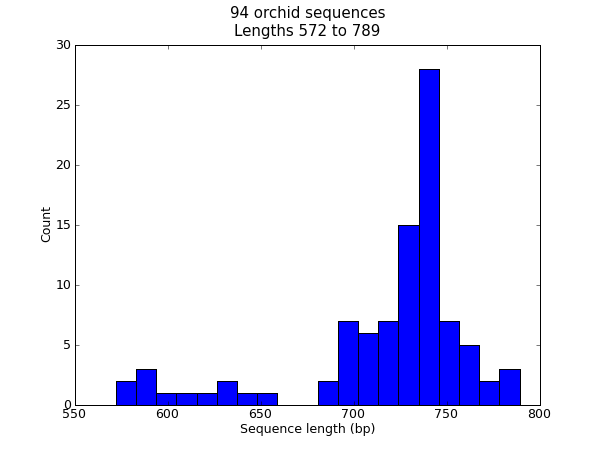
\includegraphics{hist_plot.png}

注意,这些兰花序列的长度大多数大约在740bp左右,这里有可能有两个不同长度的序列分类,其中包含一个较短的序列子集。

\emph{提示:} 除了使用 \code{pylab.show()} 在窗口中显示图像以外,你也可以使用 \code{pylab.savefig(...)} 来将图像保存为图像文件中(例如PNG或PDF文件)。


\subsection{18.2.2  序列GC\%含量作图}
\label{chr18:gc}
对于核酸序列,另一个经常计算的值是GC含量。例如,你可能想要查看一个细菌基因组中所有基因的GC\%,并研究任何离群值来确定可能最近通过基因水平转移而获得的基因。同样,对于这个例子,我们再次使用兰花FASTA文件 \href{http://biopython.org/DIST/docs/tutorial/examples/ls\_orchid.fasta}{ls\_orchid.fasta} 。

首先,我们使用 \code{Bio.SeqIO} 解析这个FASTA文件并创建一个GC百分含量的列表。你可以使用for循环,但我更喜欢这样:
\DUspan{keyword,namespace}{}\DUspan{name,namespace}{}\DUspan{keyword,namespace}{}\DUspan{name}{}\DUspan{keyword,namespace}{}\DUspan{name,namespace}{}\DUspan{keyword,namespace}{}\DUspan{name}{}\DUspan{name}{}\DUspan{operator}{}\DUspan{name,builtin}{}\DUspan{punctuation}{}\DUspan{name}{}\DUspan{punctuation}{}\DUspan{name}{}\DUspan{operator}{}\DUspan{name}{}\DUspan{punctuation}{}\DUspan{keyword}{}\DUspan{name}{}\DUspan{operator,word}{}\DUspan{name}{}\DUspan{operator}{}\DUspan{name}{}\DUspan{punctuation}{}\DUspan{literal,string}{}\DUspan{punctuation}{}\DUspan{literal,string}{}\DUspan{punctuation}{}
\begin{Verbatim}[commandchars=\\\{\}]
\PYG{k+kn}{from} \PYG{n+nn}{Bio} \PYG{k+kn}{import} \PYG{n}{SeqIO}
\PYG{k+kn}{from} \PYG{n+nn}{Bio.SeqUtils} \PYG{k+kn}{import} \PYG{n}{GC}

\PYG{n}{gc\PYGZus{}values} \PYG{o}{=} \PYG{n+nb}{sorted}\PYG{p}{(}\PYG{n}{GC}\PYG{p}{(}\PYG{n}{rec}\PYG{o}{.}\PYG{n}{seq}\PYG{p}{)} \PYG{k}{for} \PYG{n}{rec} \PYG{o+ow}{in} \PYG{n}{SeqIO}\PYG{o}{.}\PYG{n}{parse}\PYG{p}{(}\PYG{l+s}{\PYGZdq{}}\PYG{l+s}{ls\PYGZus{}orchid.fasta}\PYG{l+s}{\PYGZdq{}}\PYG{p}{,} \PYG{l+s}{\PYGZdq{}}\PYG{l+s}{fasta}\PYG{l+s}{\PYGZdq{}}\PYG{p}{)}\PYG{p}{)}
\end{Verbatim}

读取完每个序列并计算了GC百分比,我们接着将它们按升序排列。现在,我们用matplotlib来对这个浮点数列表进行可视化:
\DUspan{keyword,namespace}{}\DUspan{name,namespace}{}\DUspan{name}{}\DUspan{operator}{}\DUspan{name}{}\DUspan{punctuation}{}\DUspan{name}{}\DUspan{punctuation}{}\DUspan{name}{}\DUspan{operator}{}\DUspan{name}{}\DUspan{punctuation}{}\DUspan{literal,string}{}\DUspan{literal,string,interpol}{}\DUspan{literal,string}{}\DUspan{literal,string,escape}{}\DUspan{literal,string}{}\DUspan{literal,string,interpol}{}\DUspan{literal,string}{}\DUspan{literal,string,interpol}{}\DUspan{literal,string}{}\DUspan{literal,string,interpol}{}\DUspan{literal,string}{}\DUspan{operator}{}\DUspan{punctuation}{}\DUspan{name,builtin}{}\DUspan{punctuation}{}\DUspan{name}{}\DUspan{punctuation}{}\DUspan{name,builtin}{}\DUspan{punctuation}{}\DUspan{name}{}\DUspan{punctuation}{}\DUspan{name,builtin}{}\DUspan{punctuation}{}\DUspan{name}{}\DUspan{punctuation}{}\DUspan{name}{}\DUspan{operator}{}\DUspan{name}{}\DUspan{punctuation}{}\DUspan{literal,string}{}\DUspan{punctuation}{}\DUspan{name}{}\DUspan{operator}{}\DUspan{name}{}\DUspan{punctuation}{}\DUspan{literal,string}{}\DUspan{punctuation}{}\DUspan{name}{}\DUspan{operator}{}\DUspan{name}{}\DUspan{punctuation}{}
\begin{Verbatim}[commandchars=\\\{\}]
\PYG{k+kn}{import} \PYG{n+nn}{pylab}
\PYG{n}{pylab}\PYG{o}{.}\PYG{n}{plot}\PYG{p}{(}\PYG{n}{gc\PYGZus{}values}\PYG{p}{)}
\PYG{n}{pylab}\PYG{o}{.}\PYG{n}{title}\PYG{p}{(}\PYG{l+s}{\PYGZdq{}}\PYG{l+s+si}{\PYGZpc{}i}\PYG{l+s}{ orchid sequences}\PYG{l+s+se}{\PYGZbs{}n}\PYG{l+s}{GC}\PYG{l+s+si}{\PYGZpc{}\PYGZpc{}}\PYG{l+s}{ }\PYG{l+s+si}{\PYGZpc{}0.1f}\PYG{l+s}{ to }\PYG{l+s+si}{\PYGZpc{}0.1f}\PYG{l+s}{\PYGZdq{}} \PYGZbs{}
            \PYG{o}{\PYGZpc{}} \PYG{p}{(}\PYG{n+nb}{len}\PYG{p}{(}\PYG{n}{gc\PYGZus{}values}\PYG{p}{)}\PYG{p}{,}\PYG{n+nb}{min}\PYG{p}{(}\PYG{n}{gc\PYGZus{}values}\PYG{p}{)}\PYG{p}{,}\PYG{n+nb}{max}\PYG{p}{(}\PYG{n}{gc\PYGZus{}values}\PYG{p}{)}\PYG{p}{)}\PYG{p}{)}
\PYG{n}{pylab}\PYG{o}{.}\PYG{n}{xlabel}\PYG{p}{(}\PYG{l+s}{\PYGZdq{}}\PYG{l+s}{Genes}\PYG{l+s}{\PYGZdq{}}\PYG{p}{)}
\PYG{n}{pylab}\PYG{o}{.}\PYG{n}{ylabel}\PYG{p}{(}\PYG{l+s}{\PYGZdq{}}\PYG{l+s}{GC}\PYG{l+s}{\PYGZpc{}}\PYG{l+s}{\PYGZdq{}}\PYG{p}{)}
\PYG{n}{pylab}\PYG{o}{.}\PYG{n}{show}\PYG{p}{(}\PYG{p}{)}
\end{Verbatim}

像之前的例子一样,弹出一个窗口中将包含如下图形:

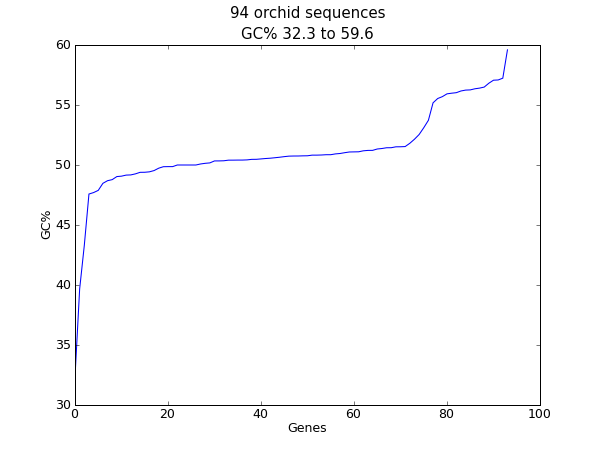
\includegraphics{gc_plot.png}

如果你使用的是一个物种中的所有基因集,你可能会得到一个更加平滑的图。


\subsection{18.2.3  核苷酸点线图}
\label{chr18:id12}
点线图是可视化比较两条核苷酸序列的相似性的一种方式。采用一个滑动窗来相互比较较短的子序列(比较通常根据一个不匹配阈值来实现)。为了简单起见,此处我们将只查找完全匹配(如下图黑色所示)。

我们需要两条序列开始。为了论证,我们只取兰花FASTA文件中的前两条序列。\href{http://biopython.org/DIST/docs/tutorial/examples/ls\_orchid.fasta}{ls\_orchid.fasta}:
\DUspan{keyword,namespace}{}\DUspan{name,namespace}{}\DUspan{keyword,namespace}{}\DUspan{name}{}\DUspan{name}{}\DUspan{operator}{}\DUspan{name,builtin}{}\DUspan{punctuation}{}\DUspan{literal,string}{}\DUspan{punctuation}{}\DUspan{name}{}\DUspan{operator}{}\DUspan{name}{}\DUspan{operator}{}\DUspan{name}{}\DUspan{punctuation}{}\DUspan{name}{}\DUspan{punctuation}{}\DUspan{literal,string}{}\DUspan{punctuation}{}\DUspan{name}{}\DUspan{operator}{}\DUspan{name}{}\DUspan{operator}{}\DUspan{name}{}\DUspan{punctuation}{}\DUspan{name}{}\DUspan{operator}{}\DUspan{name}{}\DUspan{operator}{}\DUspan{name}{}\DUspan{punctuation}{}\DUspan{name}{}\DUspan{operator}{}\DUspan{name}{}\DUspan{punctuation}{}
\begin{Verbatim}[commandchars=\\\{\}]
\PYG{k+kn}{from} \PYG{n+nn}{Bio} \PYG{k+kn}{import} \PYG{n}{SeqIO}
\PYG{n}{handle} \PYG{o}{=} \PYG{n+nb}{open}\PYG{p}{(}\PYG{l+s}{\PYGZdq{}}\PYG{l+s}{ls\PYGZus{}orchid.fasta}\PYG{l+s}{\PYGZdq{}}\PYG{p}{)}
\PYG{n}{record\PYGZus{}iterator} \PYG{o}{=} \PYG{n}{SeqIO}\PYG{o}{.}\PYG{n}{parse}\PYG{p}{(}\PYG{n}{handle}\PYG{p}{,} \PYG{l+s}{\PYGZdq{}}\PYG{l+s}{fasta}\PYG{l+s}{\PYGZdq{}}\PYG{p}{)}
\PYG{n}{rec\PYGZus{}one} \PYG{o}{=} \PYG{n}{record\PYGZus{}iterator}\PYG{o}{.}\PYG{n}{next}\PYG{p}{(}\PYG{p}{)}
\PYG{n}{rec\PYGZus{}two} \PYG{o}{=} \PYG{n}{record\PYGZus{}iterator}\PYG{o}{.}\PYG{n}{next}\PYG{p}{(}\PYG{p}{)}
\PYG{n}{handle}\PYG{o}{.}\PYG{n}{close}\PYG{p}{(}\PYG{p}{)}
\end{Verbatim}

我们将展示两种方式。首先,一个简单的实现,它将所有滑动窗大小的子序列相互比较,并生产一个相似性矩阵。你可以创建一个矩阵或数组对象,而在这儿,我们只用一个用嵌套的列表解析生成的布尔值列表的列表。
\DUspan{name}{}\DUspan{operator}{}\DUspan{literal,number,integer}{}\DUspan{name}{}\DUspan{operator}{}\DUspan{name,builtin}{}\DUspan{punctuation}{}\DUspan{name}{}\DUspan{operator}{}\DUspan{name}{}\DUspan{punctuation}{}\DUspan{operator}{}\DUspan{name}{}\DUspan{punctuation}{}\DUspan{name}{}\DUspan{operator}{}\DUspan{name,builtin}{}\DUspan{punctuation}{}\DUspan{name}{}\DUspan{operator}{}\DUspan{name}{}\DUspan{punctuation}{}\DUspan{operator}{}\DUspan{name}{}\DUspan{punctuation}{}\DUspan{name}{}\DUspan{operator}{}\DUspan{punctuation}{}\DUspan{name}{}\DUspan{punctuation}{}\DUspan{name}{}\DUspan{punctuation}{}\DUspan{name}{}\DUspan{operator}{}\DUspan{name}{}\DUspan{punctuation}{}\DUspan{operator}{}\DUspan{name}{}\DUspan{punctuation}{}\DUspan{name}{}\DUspan{punctuation}{}\DUspan{name}{}\DUspan{operator}{}\DUspan{name}{}\DUspan{punctuation}{}\DUspan{keyword}{}\DUspan{name}{}\DUspan{operator,word}{}\DUspan{name,builtin}{}\DUspan{punctuation}{}\DUspan{name,builtin}{}\DUspan{punctuation}{}\DUspan{name}{}\DUspan{punctuation}{}\DUspan{operator}{}\DUspan{name}{}\DUspan{punctuation}{}\DUspan{keyword}{}\DUspan{name}{}\DUspan{operator,word}{}\DUspan{name,builtin}{}\DUspan{punctuation}{}\DUspan{name,builtin}{}\DUspan{punctuation}{}\DUspan{name}{}\DUspan{punctuation}{}\DUspan{operator}{}\DUspan{name}{}\DUspan{punctuation}{}
\begin{Verbatim}[commandchars=\\\{\}]
\PYG{n}{window} \PYG{o}{=} \PYG{l+m+mi}{7}
\PYG{n}{seq\PYGZus{}one} \PYG{o}{=} \PYG{n+nb}{str}\PYG{p}{(}\PYG{n}{rec\PYGZus{}one}\PYG{o}{.}\PYG{n}{seq}\PYG{p}{)}\PYG{o}{.}\PYG{n}{upper}\PYG{p}{(}\PYG{p}{)}
\PYG{n}{seq\PYGZus{}two} \PYG{o}{=} \PYG{n+nb}{str}\PYG{p}{(}\PYG{n}{rec\PYGZus{}two}\PYG{o}{.}\PYG{n}{seq}\PYG{p}{)}\PYG{o}{.}\PYG{n}{upper}\PYG{p}{(}\PYG{p}{)}
\PYG{n}{data} \PYG{o}{=} \PYG{p}{[}\PYG{p}{[}\PYG{p}{(}\PYG{n}{seq\PYGZus{}one}\PYG{p}{[}\PYG{n}{i}\PYG{p}{:}\PYG{n}{i}\PYG{o}{+}\PYG{n}{window}\PYG{p}{]} \PYG{o}{\PYGZlt{}}\PYG{o}{\PYGZgt{}} \PYG{n}{seq\PYGZus{}two}\PYG{p}{[}\PYG{n}{j}\PYG{p}{:}\PYG{n}{j}\PYG{o}{+}\PYG{n}{window}\PYG{p}{]}\PYG{p}{)} \PYGZbs{}
        \PYG{k}{for} \PYG{n}{j} \PYG{o+ow}{in} \PYG{n+nb}{range}\PYG{p}{(}\PYG{n+nb}{len}\PYG{p}{(}\PYG{n}{seq\PYGZus{}one}\PYG{p}{)}\PYG{o}{\PYGZhy{}}\PYG{n}{window}\PYG{p}{)}\PYG{p}{]} \PYGZbs{}
       \PYG{k}{for} \PYG{n}{i} \PYG{o+ow}{in} \PYG{n+nb}{range}\PYG{p}{(}\PYG{n+nb}{len}\PYG{p}{(}\PYG{n}{seq\PYGZus{}two}\PYG{p}{)}\PYG{o}{\PYGZhy{}}\PYG{n}{window}\PYG{p}{)}\PYG{p}{]}
\end{Verbatim}

注意,我们在这里并 \emph{没有} 检查反向的互补匹配。现在我们将使用matplotlib的 \code{pylab.imshow()} 函数来显示这个数据,首先启用灰度模式,以保证这是在黑白颜色下完成的:
\DUspan{keyword,namespace}{}\DUspan{name,namespace}{}\DUspan{name}{}\DUspan{operator}{}\DUspan{name}{}\DUspan{punctuation}{}\DUspan{name}{}\DUspan{operator}{}\DUspan{name}{}\DUspan{punctuation}{}\DUspan{name}{}\DUspan{punctuation}{}\DUspan{name}{}\DUspan{operator}{}\DUspan{name}{}\DUspan{punctuation}{}\DUspan{literal,string}{}\DUspan{literal,string,interpol}{}\DUspan{literal,string}{}\DUspan{literal,string,interpol}{}\DUspan{literal,string}{}\DUspan{operator}{}\DUspan{punctuation}{}\DUspan{name}{}\DUspan{operator}{}\DUspan{name}{}\DUspan{punctuation}{}\DUspan{name,builtin}{}\DUspan{punctuation}{}\DUspan{name}{}\DUspan{punctuation}{}\DUspan{name}{}\DUspan{operator}{}\DUspan{name}{}\DUspan{punctuation}{}\DUspan{literal,string}{}\DUspan{literal,string,interpol}{}\DUspan{literal,string}{}\DUspan{literal,string,interpol}{}\DUspan{literal,string}{}\DUspan{operator}{}\DUspan{punctuation}{}\DUspan{name}{}\DUspan{operator}{}\DUspan{name}{}\DUspan{punctuation}{}\DUspan{name,builtin}{}\DUspan{punctuation}{}\DUspan{name}{}\DUspan{punctuation}{}\DUspan{name}{}\DUspan{operator}{}\DUspan{name}{}\DUspan{punctuation}{}\DUspan{literal,string}{}\DUspan{literal,string,interpol}{}\DUspan{literal,string,escape}{}\DUspan{literal,string}{}\DUspan{operator}{}\DUspan{name}{}\DUspan{punctuation}{}\DUspan{name}{}\DUspan{operator}{}\DUspan{name}{}\DUspan{punctuation}{}
\begin{Verbatim}[commandchars=\\\{\}]
\PYG{k+kn}{import} \PYG{n+nn}{pylab}
\PYG{n}{pylab}\PYG{o}{.}\PYG{n}{gray}\PYG{p}{(}\PYG{p}{)}
\PYG{n}{pylab}\PYG{o}{.}\PYG{n}{imshow}\PYG{p}{(}\PYG{n}{data}\PYG{p}{)}
\PYG{n}{pylab}\PYG{o}{.}\PYG{n}{xlabel}\PYG{p}{(}\PYG{l+s}{\PYGZdq{}}\PYG{l+s+si}{\PYGZpc{}s}\PYG{l+s}{ (length }\PYG{l+s+si}{\PYGZpc{}i}\PYG{l+s}{ bp)}\PYG{l+s}{\PYGZdq{}} \PYG{o}{\PYGZpc{}} \PYG{p}{(}\PYG{n}{rec\PYGZus{}one}\PYG{o}{.}\PYG{n}{id}\PYG{p}{,} \PYG{n+nb}{len}\PYG{p}{(}\PYG{n}{rec\PYGZus{}one}\PYG{p}{)}\PYG{p}{)}\PYG{p}{)}
\PYG{n}{pylab}\PYG{o}{.}\PYG{n}{ylabel}\PYG{p}{(}\PYG{l+s}{\PYGZdq{}}\PYG{l+s+si}{\PYGZpc{}s}\PYG{l+s}{ (length }\PYG{l+s+si}{\PYGZpc{}i}\PYG{l+s}{ bp)}\PYG{l+s}{\PYGZdq{}} \PYG{o}{\PYGZpc{}} \PYG{p}{(}\PYG{n}{rec\PYGZus{}two}\PYG{o}{.}\PYG{n}{id}\PYG{p}{,} \PYG{n+nb}{len}\PYG{p}{(}\PYG{n}{rec\PYGZus{}two}\PYG{p}{)}\PYG{p}{)}\PYG{p}{)}
\PYG{n}{pylab}\PYG{o}{.}\PYG{n}{title}\PYG{p}{(}\PYG{l+s}{\PYGZdq{}}\PYG{l+s}{Dot plot using window size }\PYG{l+s+si}{\PYGZpc{}i}\PYG{l+s+se}{\PYGZbs{}n}\PYG{l+s}{(allowing no mis\PYGZhy{}matches)}\PYG{l+s}{\PYGZdq{}} \PYG{o}{\PYGZpc{}} \PYG{n}{window}\PYG{p}{)}
\PYG{n}{pylab}\PYG{o}{.}\PYG{n}{show}\PYG{p}{(}\PYG{p}{)}
\end{Verbatim}

这将弹出一个新的窗口,包含类似这样的图形:

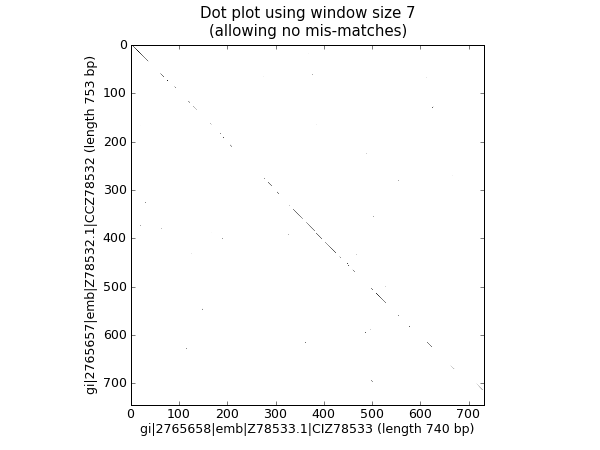
\includegraphics{dot_plot.png}

可能如您所料,这两条序列非常相似,图中部分滑动窗大小的线沿着对角线匹配。图中没有对角线外的点,这意味着序列中并没有倒位或其他有趣的偏离对角线匹配。

上面的代码在小的例子中工作得很好,但是应用到大的序列时,这里有两个问题。首先,这种以穷举地方式进行所有可能的两两比对非常缓慢。作为替代,我们将创建一个词典来映射所有滑动窗大小的子序列的位置,然后取两者的交集来获得两条序列中都发现的子序列。这将占用更多的内存,然而速度 \emph{更} 快。另外, \code{pylab.imshow()} 函数只能显示较小的矩阵。作为替代,我们将使用 \code{pylab.scatter()} 函数。

我们从创建,从滑动窗大小的子序列到其位置的字典映射开始:
\DUspan{name}{}\DUspan{operator}{}\DUspan{literal,number,integer}{}\DUspan{name}{}\DUspan{operator}{}\DUspan{punctuation}{}\DUspan{name}{}\DUspan{operator}{}\DUspan{punctuation}{}\DUspan{keyword}{}\DUspan{punctuation}{}\DUspan{name}{}\DUspan{punctuation}{}\DUspan{name}{}\DUspan{punctuation}{}\DUspan{operator,word}{}\DUspan{punctuation}{}\DUspan{name,builtin}{}\DUspan{punctuation}{}\DUspan{name}{}\DUspan{operator}{}\DUspan{name}{}\DUspan{punctuation}{}\DUspan{operator}{}\DUspan{name}{}\DUspan{punctuation}{}\DUspan{name}{}\DUspan{punctuation}{}\DUspan{punctuation}{}\DUspan{name,builtin}{}\DUspan{punctuation}{}\DUspan{name}{}\DUspan{operator}{}\DUspan{name}{}\DUspan{punctuation}{}\DUspan{operator}{}\DUspan{name}{}\DUspan{punctuation}{}\DUspan{name}{}\DUspan{punctuation}{}\DUspan{keyword}{}\DUspan{name}{}\DUspan{operator,word}{}\DUspan{name,builtin}{}\DUspan{punctuation}{}\DUspan{name,builtin}{}\DUspan{punctuation}{}\DUspan{name}{}\DUspan{punctuation}{}\DUspan{operator}{}\DUspan{name}{}\DUspan{punctuation}{}\DUspan{name}{}\DUspan{operator}{}\DUspan{name}{}\DUspan{punctuation}{}\DUspan{name}{}\DUspan{punctuation}{}\DUspan{name}{}\DUspan{operator}{}\DUspan{name}{}\DUspan{punctuation}{}\DUspan{keyword}{}\DUspan{punctuation}{}\DUspan{name}{}\DUspan{punctuation}{}\DUspan{name}{}\DUspan{punctuation}{}\DUspan{operator}{}\DUspan{name}{}\DUspan{punctuation}{}\DUspan{name}{}\DUspan{punctuation}{}\DUspan{keyword}{}\DUspan{name,exception}{}\DUspan{punctuation}{}\DUspan{name}{}\DUspan{punctuation}{}\DUspan{name}{}\DUspan{punctuation}{}\DUspan{operator}{}\DUspan{punctuation}{}\DUspan{name}{}\DUspan{punctuation}{}\DUspan{comment}{}\DUspan{comment}{}\DUspan{name}{}\DUspan{operator}{}\DUspan{name,builtin}{}\DUspan{punctuation}{}\DUspan{name}{}\DUspan{punctuation}{}\DUspan{operator}{}\DUspan{name}{}\DUspan{punctuation}{}\DUspan{name}{}\DUspan{punctuation}{}\DUspan{keyword}{}\DUspan{literal,string}{}\DUspan{literal,string,interpol}{}\DUspan{literal,string}{}\DUspan{operator}{}\DUspan{name,builtin}{}\DUspan{punctuation}{}\DUspan{name}{}\DUspan{punctuation}{}
\begin{Verbatim}[commandchars=\\\{\}]
\PYG{n}{window} \PYG{o}{=} \PYG{l+m+mi}{7}
\PYG{n}{dict\PYGZus{}one} \PYG{o}{=} \PYG{p}{\PYGZob{}}\PYG{p}{\PYGZcb{}}
\PYG{n}{dict\PYGZus{}two} \PYG{o}{=} \PYG{p}{\PYGZob{}}\PYG{p}{\PYGZcb{}}
\PYG{k}{for} \PYG{p}{(}\PYG{n}{seq}\PYG{p}{,} \PYG{n}{section\PYGZus{}dict}\PYG{p}{)} \PYG{o+ow}{in} \PYG{p}{[}\PYG{p}{(}\PYG{n+nb}{str}\PYG{p}{(}\PYG{n}{rec\PYGZus{}one}\PYG{o}{.}\PYG{n}{seq}\PYG{p}{)}\PYG{o}{.}\PYG{n}{upper}\PYG{p}{(}\PYG{p}{)}\PYG{p}{,} \PYG{n}{dict\PYGZus{}one}\PYG{p}{)}\PYG{p}{,}
                            \PYG{p}{(}\PYG{n+nb}{str}\PYG{p}{(}\PYG{n}{rec\PYGZus{}two}\PYG{o}{.}\PYG{n}{seq}\PYG{p}{)}\PYG{o}{.}\PYG{n}{upper}\PYG{p}{(}\PYG{p}{)}\PYG{p}{,} \PYG{n}{dict\PYGZus{}two}\PYG{p}{)}\PYG{p}{]}\PYG{p}{:}
    \PYG{k}{for} \PYG{n}{i} \PYG{o+ow}{in} \PYG{n+nb}{range}\PYG{p}{(}\PYG{n+nb}{len}\PYG{p}{(}\PYG{n}{seq}\PYG{p}{)}\PYG{o}{\PYGZhy{}}\PYG{n}{window}\PYG{p}{)}\PYG{p}{:}
        \PYG{n}{section} \PYG{o}{=} \PYG{n}{seq}\PYG{p}{[}\PYG{n}{i}\PYG{p}{:}\PYG{n}{i}\PYG{o}{+}\PYG{n}{window}\PYG{p}{]}
        \PYG{k}{try}\PYG{p}{:}
            \PYG{n}{section\PYGZus{}dict}\PYG{p}{[}\PYG{n}{section}\PYG{p}{]}\PYG{o}{.}\PYG{n}{append}\PYG{p}{(}\PYG{n}{i}\PYG{p}{)}
        \PYG{k}{except} \PYG{n+ne}{KeyError}\PYG{p}{:}
            \PYG{n}{section\PYGZus{}dict}\PYG{p}{[}\PYG{n}{section}\PYG{p}{]} \PYG{o}{=} \PYG{p}{[}\PYG{n}{i}\PYG{p}{]}
\PYG{c}{\PYGZsh{}Now find any sub\PYGZhy{}sequences found in both sequences}
\PYG{c}{\PYGZsh{}(Python 2.3 would require slightly different code here)}
\PYG{n}{matches} \PYG{o}{=} \PYG{n+nb}{set}\PYG{p}{(}\PYG{n}{dict\PYGZus{}one}\PYG{p}{)}\PYG{o}{.}\PYG{n}{intersection}\PYG{p}{(}\PYG{n}{dict\PYGZus{}two}\PYG{p}{)}
\PYG{k}{print} \PYG{l+s}{\PYGZdq{}}\PYG{l+s+si}{\PYGZpc{}i}\PYG{l+s}{ unique matches}\PYG{l+s}{\PYGZdq{}} \PYG{o}{\PYGZpc{}} \PYG{n+nb}{len}\PYG{p}{(}\PYG{n}{matches}\PYG{p}{)}
\end{Verbatim}

为了使用 \code{pylab.scatter()} 函数,我们需要两个分别对应 \emph{x} 和 \emph{y} 轴的列表:
\DUspan{comment}{}\DUspan{name}{}\DUspan{operator}{}\DUspan{punctuation}{}\DUspan{name}{}\DUspan{operator}{}\DUspan{punctuation}{}\DUspan{keyword}{}\DUspan{name}{}\DUspan{operator,word}{}\DUspan{name}{}\DUspan{punctuation}{}\DUspan{keyword}{}\DUspan{name}{}\DUspan{operator,word}{}\DUspan{name}{}\DUspan{punctuation}{}\DUspan{name}{}\DUspan{punctuation}{}\DUspan{keyword}{}\DUspan{name}{}\DUspan{operator,word}{}\DUspan{name}{}\DUspan{punctuation}{}\DUspan{name}{}\DUspan{punctuation}{}\DUspan{name}{}\DUspan{operator}{}\DUspan{name}{}\DUspan{punctuation}{}\DUspan{name}{}\DUspan{punctuation}{}\DUspan{name}{}\DUspan{operator}{}\DUspan{name}{}\DUspan{punctuation}{}\DUspan{name}{}\DUspan{punctuation}{}
\begin{Verbatim}[commandchars=\\\{\}]
\PYG{c}{\PYGZsh{}Create lists of x and y co\PYGZhy{}ordinates for scatter plot}
\PYG{n}{x} \PYG{o}{=} \PYG{p}{[}\PYG{p}{]}
\PYG{n}{y} \PYG{o}{=} \PYG{p}{[}\PYG{p}{]}
\PYG{k}{for} \PYG{n}{section} \PYG{o+ow}{in} \PYG{n}{matches}\PYG{p}{:}
    \PYG{k}{for} \PYG{n}{i} \PYG{o+ow}{in} \PYG{n}{dict\PYGZus{}one}\PYG{p}{[}\PYG{n}{section}\PYG{p}{]}\PYG{p}{:}
        \PYG{k}{for} \PYG{n}{j} \PYG{o+ow}{in} \PYG{n}{dict\PYGZus{}two}\PYG{p}{[}\PYG{n}{section}\PYG{p}{]}\PYG{p}{:}
            \PYG{n}{x}\PYG{o}{.}\PYG{n}{append}\PYG{p}{(}\PYG{n}{i}\PYG{p}{)}
            \PYG{n}{y}\PYG{o}{.}\PYG{n}{append}\PYG{p}{(}\PYG{n}{j}\PYG{p}{)}
\end{Verbatim}

现在我们能以散点图的形式画出优化后的点线图:
\DUspan{keyword,namespace}{}\DUspan{name,namespace}{}\DUspan{name}{}\DUspan{operator}{}\DUspan{name}{}\DUspan{punctuation}{}\DUspan{comment}{}\DUspan{name}{}\DUspan{operator}{}\DUspan{name}{}\DUspan{punctuation}{}\DUspan{name}{}\DUspan{operator}{}\DUspan{name}{}\DUspan{punctuation}{}\DUspan{name}{}\DUspan{punctuation}{}\DUspan{name}{}\DUspan{punctuation}{}\DUspan{name}{}\DUspan{operator}{}\DUspan{name}{}\DUspan{punctuation}{}\DUspan{literal,number,integer}{}\DUspan{punctuation}{}\DUspan{name,builtin}{}\DUspan{punctuation}{}\DUspan{name}{}\DUspan{punctuation}{}\DUspan{operator}{}\DUspan{name}{}\DUspan{punctuation}{}\DUspan{name}{}\DUspan{operator}{}\DUspan{name}{}\DUspan{punctuation}{}\DUspan{literal,number,integer}{}\DUspan{punctuation}{}\DUspan{name,builtin}{}\DUspan{punctuation}{}\DUspan{name}{}\DUspan{punctuation}{}\DUspan{operator}{}\DUspan{name}{}\DUspan{punctuation}{}\DUspan{name}{}\DUspan{operator}{}\DUspan{name}{}\DUspan{punctuation}{}\DUspan{literal,string}{}\DUspan{literal,string,interpol}{}\DUspan{literal,string}{}\DUspan{literal,string,interpol}{}\DUspan{literal,string}{}\DUspan{operator}{}\DUspan{punctuation}{}\DUspan{name}{}\DUspan{operator}{}\DUspan{name}{}\DUspan{punctuation}{}\DUspan{name,builtin}{}\DUspan{punctuation}{}\DUspan{name}{}\DUspan{punctuation}{}\DUspan{name}{}\DUspan{operator}{}\DUspan{name}{}\DUspan{punctuation}{}\DUspan{literal,string}{}\DUspan{literal,string,interpol}{}\DUspan{literal,string}{}\DUspan{literal,string,interpol}{}\DUspan{literal,string}{}\DUspan{operator}{}\DUspan{punctuation}{}\DUspan{name}{}\DUspan{operator}{}\DUspan{name}{}\DUspan{punctuation}{}\DUspan{name,builtin}{}\DUspan{punctuation}{}\DUspan{name}{}\DUspan{punctuation}{}\DUspan{name}{}\DUspan{operator}{}\DUspan{name}{}\DUspan{punctuation}{}\DUspan{literal,string}{}\DUspan{literal,string,interpol}{}\DUspan{literal,string,escape}{}\DUspan{literal,string}{}\DUspan{operator}{}\DUspan{name}{}\DUspan{punctuation}{}\DUspan{name}{}\DUspan{operator}{}\DUspan{name}{}\DUspan{punctuation}{}
\begin{Verbatim}[commandchars=\\\{\}]
\PYG{k+kn}{import} \PYG{n+nn}{pylab}
\PYG{n}{pylab}\PYG{o}{.}\PYG{n}{cla}\PYG{p}{(}\PYG{p}{)} \PYG{c}{\PYGZsh{}clear any prior graph}
\PYG{n}{pylab}\PYG{o}{.}\PYG{n}{gray}\PYG{p}{(}\PYG{p}{)}
\PYG{n}{pylab}\PYG{o}{.}\PYG{n}{scatter}\PYG{p}{(}\PYG{n}{x}\PYG{p}{,}\PYG{n}{y}\PYG{p}{)}
\PYG{n}{pylab}\PYG{o}{.}\PYG{n}{xlim}\PYG{p}{(}\PYG{l+m+mi}{0}\PYG{p}{,} \PYG{n+nb}{len}\PYG{p}{(}\PYG{n}{rec\PYGZus{}one}\PYG{p}{)}\PYG{o}{\PYGZhy{}}\PYG{n}{window}\PYG{p}{)}
\PYG{n}{pylab}\PYG{o}{.}\PYG{n}{ylim}\PYG{p}{(}\PYG{l+m+mi}{0}\PYG{p}{,} \PYG{n+nb}{len}\PYG{p}{(}\PYG{n}{rec\PYGZus{}two}\PYG{p}{)}\PYG{o}{\PYGZhy{}}\PYG{n}{window}\PYG{p}{)}
\PYG{n}{pylab}\PYG{o}{.}\PYG{n}{xlabel}\PYG{p}{(}\PYG{l+s}{\PYGZdq{}}\PYG{l+s+si}{\PYGZpc{}s}\PYG{l+s}{ (length }\PYG{l+s+si}{\PYGZpc{}i}\PYG{l+s}{ bp)}\PYG{l+s}{\PYGZdq{}} \PYG{o}{\PYGZpc{}} \PYG{p}{(}\PYG{n}{rec\PYGZus{}one}\PYG{o}{.}\PYG{n}{id}\PYG{p}{,} \PYG{n+nb}{len}\PYG{p}{(}\PYG{n}{rec\PYGZus{}one}\PYG{p}{)}\PYG{p}{)}\PYG{p}{)}
\PYG{n}{pylab}\PYG{o}{.}\PYG{n}{ylabel}\PYG{p}{(}\PYG{l+s}{\PYGZdq{}}\PYG{l+s+si}{\PYGZpc{}s}\PYG{l+s}{ (length }\PYG{l+s+si}{\PYGZpc{}i}\PYG{l+s}{ bp)}\PYG{l+s}{\PYGZdq{}} \PYG{o}{\PYGZpc{}} \PYG{p}{(}\PYG{n}{rec\PYGZus{}two}\PYG{o}{.}\PYG{n}{id}\PYG{p}{,} \PYG{n+nb}{len}\PYG{p}{(}\PYG{n}{rec\PYGZus{}two}\PYG{p}{)}\PYG{p}{)}\PYG{p}{)}
\PYG{n}{pylab}\PYG{o}{.}\PYG{n}{title}\PYG{p}{(}\PYG{l+s}{\PYGZdq{}}\PYG{l+s}{Dot plot using window size }\PYG{l+s+si}{\PYGZpc{}i}\PYG{l+s+se}{\PYGZbs{}n}\PYG{l+s}{(allowing no mis\PYGZhy{}matches)}\PYG{l+s}{\PYGZdq{}} \PYG{o}{\PYGZpc{}} \PYG{n}{window}\PYG{p}{)}
\PYG{n}{pylab}\PYG{o}{.}\PYG{n}{show}\PYG{p}{(}\PYG{p}{)}
\end{Verbatim}

这将弹出一个新的窗口,包含如下图形:

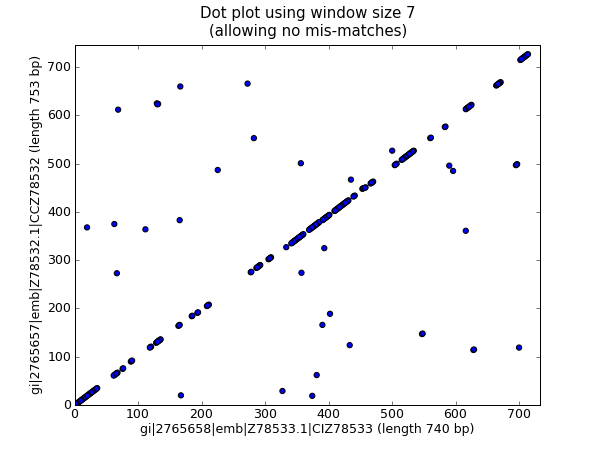
\includegraphics{dot_plot_scatter.png}

我个人认为第二个图更加易读!再次注意,我们在这里 \emph{没有} 检查反向互补匹配 —— 你可以扩展这个例子来实现它,或许可以以一种颜色显示正向匹配,另一种显示反向匹配。


\subsection{18.2.4  绘制序列读长数据的质量图}
\label{chr18:id13}
如果你在处理二代测序数据,你可能希望绘制数据的质量图。这里使用两个包含双末端(paired end)读长的FASTQ文件作为例子,其中 \code{SRR001666\_1.fastq} 为正向读长, \code{SRR001666\_2.fastq} 为反向读长。它们可以从ENA序列读长档案的FTP站点下载( \href{ftp://ftp.sra.ebi.ac.uk/vol1/fastq/SRR001/SRR001666/SRR001666\_1.fastq.gz}{ftp://ftp.sra.ebi.ac.uk/vol1/fastq/SRR001/SRR001666/SRR001666\_1.fastq.gz} 和 \href{ftp://ftp.sra.ebi.ac.uk/vol1/fastq/SRR001/SRR001666/SRR001666\_2.fastq.gz}{ftp://ftp.sra.ebi.ac.uk/vol1/fastq/SRR001/SRR001666/SRR001666\_2.fastq.gz} ), 且来自 \emph{E. coli} —— 参见 \href{http://www.ebi.ac.uk/ena/data/view/SRR001666}{http://www.ebi.ac.uk/ena/data/view/SRR001666} 的详细介绍。在下面的代码中, \code{pylab.subplot(...)} 函数被用来在两个子图中展示正向和反向的质量。这里也有少量的代码来保证仅仅展示前50个读长的质量。
\DUspan{keyword,namespace}{}\DUspan{name,namespace}{}\DUspan{keyword,namespace}{}\DUspan{name,namespace}{}\DUspan{keyword,namespace}{}\DUspan{name}{}\DUspan{keyword}{}\DUspan{name}{}\DUspan{operator,word}{}\DUspan{punctuation}{}\DUspan{literal,number,integer}{}\DUspan{punctuation}{}\DUspan{literal,number,integer}{}\DUspan{punctuation}{}\DUspan{name}{}\DUspan{operator}{}\DUspan{literal,string}{}\DUspan{literal,string,interpol}{}\DUspan{literal,string}{}\DUspan{operator}{}\DUspan{name}{}\DUspan{name}{}\DUspan{operator}{}\DUspan{name}{}\DUspan{punctuation}{}\DUspan{literal,number,integer}{}\DUspan{punctuation}{}\DUspan{literal,number,integer}{}\DUspan{punctuation}{}\DUspan{name}{}\DUspan{punctuation}{}\DUspan{keyword}{}\DUspan{name}{}\DUspan{punctuation}{}\DUspan{name}{}\DUspan{operator,word}{}\DUspan{name,builtin}{}\DUspan{punctuation}{}\DUspan{name}{}\DUspan{operator}{}\DUspan{name}{}\DUspan{punctuation}{}\DUspan{name}{}\DUspan{punctuation}{}\DUspan{literal,string}{}\DUspan{punctuation}{}\DUspan{keyword}{}\DUspan{name}{}\DUspan{operator}{}\DUspan{literal,number,integer}{}\DUspan{punctuation}{}\DUspan{keyword}{}\DUspan{comment}{}\DUspan{name}{}\DUspan{operator}{}\DUspan{name}{}\DUspan{punctuation}{}\DUspan{name}{}\DUspan{operator}{}\DUspan{name}{}\DUspan{punctuation}{}\DUspan{literal,string}{}\DUspan{punctuation}{}\DUspan{name}{}\DUspan{operator}{}\DUspan{name}{}\DUspan{punctuation}{}\DUspan{literal,number,integer}{}\DUspan{punctuation}{}\DUspan{literal,number,integer}{}\DUspan{punctuation}{}\DUspan{name}{}\DUspan{operator}{}\DUspan{name}{}\DUspan{punctuation}{}\DUspan{literal,string}{}\DUspan{punctuation}{}\DUspan{name}{}\DUspan{operator}{}\DUspan{name}{}\DUspan{punctuation}{}\DUspan{literal,string}{}\DUspan{punctuation}{}\DUspan{name}{}\DUspan{operator}{}\DUspan{name}{}\DUspan{punctuation}{}\DUspan{literal,string}{}\DUspan{punctuation}{}\DUspan{keyword}{}\DUspan{literal,string}{}
\begin{Verbatim}[commandchars=\\\{\}]
\PYG{k+kn}{import} \PYG{n+nn}{pylab}
\PYG{k+kn}{from} \PYG{n+nn}{Bio} \PYG{k+kn}{import} \PYG{n}{SeqIO}
\PYG{k}{for} \PYG{n}{subfigure} \PYG{o+ow}{in} \PYG{p}{[}\PYG{l+m+mi}{1}\PYG{p}{,}\PYG{l+m+mi}{2}\PYG{p}{]}\PYG{p}{:}
    \PYG{n}{filename} \PYG{o}{=} \PYG{l+s}{\PYGZdq{}}\PYG{l+s}{SRR001666\PYGZus{}}\PYG{l+s+si}{\PYGZpc{}i}\PYG{l+s}{.fastq}\PYG{l+s}{\PYGZdq{}} \PYG{o}{\PYGZpc{}} \PYG{n}{subfigure}
    \PYG{n}{pylab}\PYG{o}{.}\PYG{n}{subplot}\PYG{p}{(}\PYG{l+m+mi}{1}\PYG{p}{,} \PYG{l+m+mi}{2}\PYG{p}{,} \PYG{n}{subfigure}\PYG{p}{)}
    \PYG{k}{for} \PYG{n}{i}\PYG{p}{,}\PYG{n}{record} \PYG{o+ow}{in} \PYG{n+nb}{enumerate}\PYG{p}{(}\PYG{n}{SeqIO}\PYG{o}{.}\PYG{n}{parse}\PYG{p}{(}\PYG{n}{filename}\PYG{p}{,} \PYG{l+s}{\PYGZdq{}}\PYG{l+s}{fastq}\PYG{l+s}{\PYGZdq{}}\PYG{p}{)}\PYG{p}{)}\PYG{p}{:}
        \PYG{k}{if} \PYG{n}{i} \PYG{o}{\PYGZgt{}}\PYG{o}{=} \PYG{l+m+mi}{50} \PYG{p}{:} \PYG{k}{break} \PYG{c}{\PYGZsh{}trick!}
        \PYG{n}{pylab}\PYG{o}{.}\PYG{n}{plot}\PYG{p}{(}\PYG{n}{record}\PYG{o}{.}\PYG{n}{letter\PYGZus{}annotations}\PYG{p}{[}\PYG{l+s}{\PYGZdq{}}\PYG{l+s}{phred\PYGZus{}quality}\PYG{l+s}{\PYGZdq{}}\PYG{p}{]}\PYG{p}{)}
    \PYG{n}{pylab}\PYG{o}{.}\PYG{n}{ylim}\PYG{p}{(}\PYG{l+m+mi}{0}\PYG{p}{,}\PYG{l+m+mi}{45}\PYG{p}{)}
    \PYG{n}{pylab}\PYG{o}{.}\PYG{n}{ylabel}\PYG{p}{(}\PYG{l+s}{\PYGZdq{}}\PYG{l+s}{PHRED quality score}\PYG{l+s}{\PYGZdq{}}\PYG{p}{)}
    \PYG{n}{pylab}\PYG{o}{.}\PYG{n}{xlabel}\PYG{p}{(}\PYG{l+s}{\PYGZdq{}}\PYG{l+s}{Position}\PYG{l+s}{\PYGZdq{}}\PYG{p}{)}
\PYG{n}{pylab}\PYG{o}{.}\PYG{n}{savefig}\PYG{p}{(}\PYG{l+s}{\PYGZdq{}}\PYG{l+s}{SRR001666.png}\PYG{l+s}{\PYGZdq{}}\PYG{p}{)}
\PYG{k}{print} \PYG{l+s}{\PYGZdq{}}\PYG{l+s}{Done}\PYG{l+s}{\PYGZdq{}}
\end{Verbatim}

你应该注意到,这里我们使用了 \code{Bio.SeqIO} 的格式名称 \code{fastq} ,因为NCBI使用标准Sanger FASTQ和PHRED分数的存储这些读长。然而,你可能从读长的长度中猜到,这些数据来自Illumina Genome Analyzer,而且可能最初是以Solexa/Illumina FASTQ两种格式变种中的一种存在。

这个例子使用 \code{pylab.savefig(...)} 函数,而不是{}`{}`pylab.show(...){}`{}` ,然而就像前面提到的一样,它们两者都非常有用。下面是得到的结果:

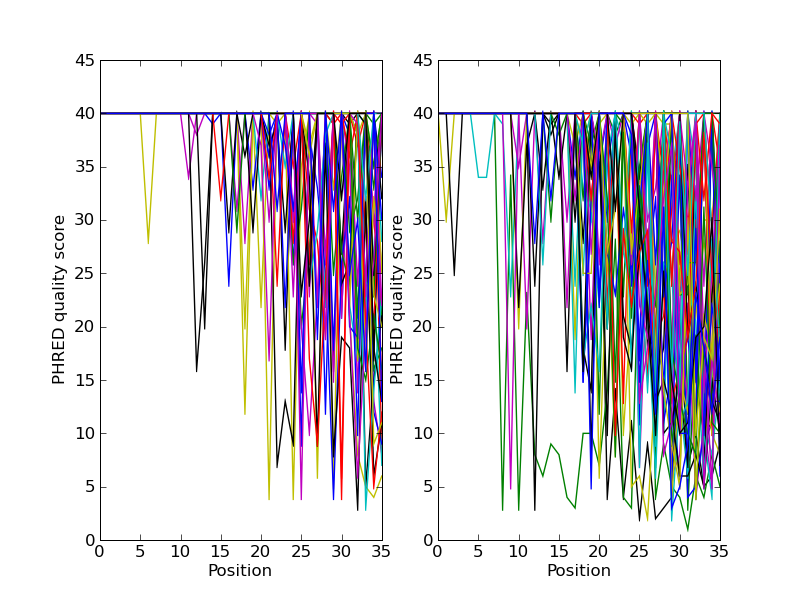
\includegraphics{SRR001666.png}


\section{18.3  处理序列比对}
\label{chr18:id14}
这部分可以看做是第 {\hyperref[chr06:chapter-bio-alignio]{\emph{6}}} 章的继续。


\subsection{18.3.1  计算摘要信息}
\label{chr18:sec-summary-info}\label{chr18:id15}
一旦你有一个比对,你很可能希望找出关于它的一些信息。我们尽力将这些功能分离到单独的能作用于比对对象的类中,而不是将所有的能生成比对信息的函数都放入比对对象本身。

准备计算比对对象的摘要信息非常快捷。假设我们已经得到了一个比对对象 \code{alignment} ,例如由在第 {\hyperref[chr06:chapter-bio-alignio]{\emph{6}}} 章介绍的 \code{Bio.AlignIO.read(...)} 读入。我们获得该对象的摘要信息所要做的所有事情是:
\DUspan{keyword,namespace}{}\DUspan{name,namespace}{}\DUspan{keyword,namespace}{}\DUspan{name}{}\DUspan{name}{}\DUspan{operator}{}\DUspan{name}{}\DUspan{operator}{}\DUspan{name}{}\DUspan{punctuation}{}\DUspan{name}{}\DUspan{punctuation}{}
\begin{Verbatim}[commandchars=\\\{\}]
\PYG{k+kn}{from} \PYG{n+nn}{Bio.Align} \PYG{k+kn}{import} \PYG{n}{AlignInfo}
\PYG{n}{summary\PYGZus{}align} \PYG{o}{=} \PYG{n}{AlignInfo}\PYG{o}{.}\PYG{n}{SummaryInfo}\PYG{p}{(}\PYG{n}{alignment}\PYG{p}{)}
\end{Verbatim}

\code{summary\_align} 对象非常有用,它将帮你做以下巧妙的事情:
\begin{enumerate}
\item {} 
计算一个快速一致序列 – 参见章节 {\hyperref[chr18:sec-consensus]{\emph{18.3.2}}}

\item {} 
获取一个针对该比对的位点特异性打分矩阵 – 参见章节 {\hyperref[chr18:sec-pssm]{\emph{18.3.3}}}

\item {} 
计算比对的信息量 – 参见章节 {\hyperref[chr18:sec-getting-info-content]{\emph{18.3.4}}}

\item {} 
生成该比对中的替换信息 – 章节 {\hyperref[chr18:sec-sub-matrix]{\emph{18.4}}} 详细描述了使用该方法生成一个替换矩阵

\end{enumerate}


\subsection{18.3.2  计算一个快速一致序列}
\label{chr18:sec-consensus}\label{chr18:id16}
在章节 {\hyperref[chr18:sec-summary-info]{\emph{18.3.1}}} 中描述的 \code{SummaryInfo} 对象提供了一个可以快速计算比对的保守(consensus)序列的功能。假设我们有一个 \code{SummaryInfo} 对象,叫做 \code{summary\_align},我们能通过下面的方法计算一个保守序列:
\DUspan{name}{}\DUspan{operator}{}\DUspan{name}{}\DUspan{operator}{}\DUspan{name}{}\DUspan{punctuation}{}
\begin{Verbatim}[commandchars=\\\{\}]
\PYG{n}{consensus} \PYG{o}{=} \PYG{n}{summary\PYGZus{}align}\PYG{o}{.}\PYG{n}{dumb\PYGZus{}consensus}\PYG{p}{(}\PYG{p}{)}
\end{Verbatim}

就行名字显示的那样,这是一个非常简单的保守序列计算器,它将只是在保守序列中累加每个位点的所有残基,如果最普遍的残基数大于某个阈值时,这个最普遍的残基将被添加到保守序列中。如果它没有到达这个阈值,将添加一个“不确定字符”。最终返回的保守序列对象是一个Seq对象,它的字母表是从组成保守序列所有序列的字母表中推断出来的。所以使用 \code{print consensus} 将给出如下信息:
\DUspan{name}{}\DUspan{name}{}\DUspan{punctuation}{}\DUspan{literal,string}{}\DUspan{operator}{}\DUspan{literal,string}{}
\begin{Verbatim}[commandchars=\\\{\}]
consensus Seq('TATACATNAAAGNAGGGGGATGCGGATAAATGGAAAGGCGAAAGAAAGAAAAAAATGAAT
...', IUPACAmbiguousDNA())
\end{Verbatim}

你可以通过传入可选参数来调整 \code{dumb\_consensus} 的工作方式:
\begin{description}
\item[{\textbf{the threshold}}] \leavevmode
这是用来设定某个残基在某个位点出现的频率超过一定阈值,才将其添加到保守序列。默认为0.7(即70\%)。

\item[{\textbf{the ambiguous character}}] \leavevmode
指定保守序列中的不确定字符。默认为’N’。

\item[{\textbf{the consensus alphabet}}] \leavevmode
指定保守序列的字母表。如果没有提供,我们将从比对序列的字母表基础上推断该字母表。

\end{description}


\subsection{18.3.3  位点特异性评分矩阵}
\label{chr18:sec-pssm}\label{chr18:id17}
位点特异性评分矩阵(Position specific score matrices,PSSMs)以另一种总结比对信息的方式(与刚才介绍的保守序列不同),这或许在某些情况下更为有用。简单来说,PSSM是一个计数矩阵。对于比对中的每一列,将所有可能出现的字母进行计数并加和。这些加和值将和一个代表序列(默认为比对中的第一条序列)一起显示出来。这个序列可能是保守序列,但也可以是比对中的任何序列。例如,对于比对,
\DUspan{name}{}\DUspan{name}{}\DUspan{operator}{}\DUspan{name}{}\DUspan{name}{}
\begin{Verbatim}[commandchars=\\\{\}]
\PYG{n}{GTATC}
\PYG{n}{AT}\PYG{o}{\PYGZhy{}}\PYG{o}{\PYGZhy{}}\PYG{n}{C}
\PYG{n}{CTGTC}
\end{Verbatim}

它的PSSM是:
\DUspan{name}{}\DUspan{name}{}\DUspan{name}{}\DUspan{name}{}\DUspan{name}{}\DUspan{literal,number,integer}{}\DUspan{literal,number,integer}{}\DUspan{literal,number,integer}{}\DUspan{literal,number,integer}{}\DUspan{name}{}\DUspan{literal,number,integer}{}\DUspan{literal,number,integer}{}\DUspan{literal,number,integer}{}\DUspan{literal,number,integer}{}\DUspan{name}{}\DUspan{literal,number,integer}{}\DUspan{literal,number,integer}{}\DUspan{literal,number,integer}{}\DUspan{literal,number,integer}{}\DUspan{name}{}\DUspan{literal,number,integer}{}\DUspan{literal,number,integer}{}\DUspan{literal,number,integer}{}\DUspan{literal,number,integer}{}\DUspan{name}{}\DUspan{literal,number,integer}{}\DUspan{literal,number,integer}{}\DUspan{literal,number,integer}{}\DUspan{literal,number,integer}{}
\begin{Verbatim}[commandchars=\\\{\}]
  G A T C
G 1 1 0 1
T 0 0 3 0
A 1 1 0 0
T 0 0 2 0
C 0 0 0 3
\end{Verbatim}

假设我们有一个比对对象叫做 \code{c\_align} ,为了获得PSSM和保守序列,我们首先得到一个摘要对象(summary object),并计算一致序列:
\DUspan{name}{}\DUspan{operator}{}\DUspan{name}{}\DUspan{operator}{}\DUspan{name}{}\DUspan{punctuation}{}\DUspan{name}{}\DUspan{punctuation}{}\DUspan{name}{}\DUspan{operator}{}\DUspan{name}{}\DUspan{operator}{}\DUspan{name}{}\DUspan{punctuation}{}
\begin{Verbatim}[commandchars=\\\{\}]
\PYG{n}{summary\PYGZus{}align} \PYG{o}{=} \PYG{n}{AlignInfo}\PYG{o}{.}\PYG{n}{SummaryInfo}\PYG{p}{(}\PYG{n}{c\PYGZus{}align}\PYG{p}{)}
\PYG{n}{consensus} \PYG{o}{=} \PYG{n}{summary\PYGZus{}align}\PYG{o}{.}\PYG{n}{dumb\PYGZus{}consensus}\PYG{p}{(}\PYG{p}{)}
\end{Verbatim}

现在,我们想创建PSSM,但是在计算中忽略任何 \code{N} 不确定残基:
\DUspan{name}{}\DUspan{operator}{}\DUspan{name}{}\DUspan{operator}{}\DUspan{name}{}\DUspan{punctuation}{}\DUspan{name}{}\DUspan{punctuation}{}\DUspan{name}{}\DUspan{operator}{}\DUspan{punctuation}{}\DUspan{literal,string}{}\DUspan{punctuation}{}
\begin{Verbatim}[commandchars=\\\{\}]
\PYG{n}{my\PYGZus{}pssm} \PYG{o}{=} \PYG{n}{summary\PYGZus{}align}\PYG{o}{.}\PYG{n}{pos\PYGZus{}specific\PYGZus{}score\PYGZus{}matrix}\PYG{p}{(}\PYG{n}{consensus}\PYG{p}{,}
                                                  \PYG{n}{chars\PYGZus{}to\PYGZus{}ignore} \PYG{o}{=} \PYG{p}{[}\PYG{l+s}{\PYGZsq{}}\PYG{l+s}{N}\PYG{l+s}{\PYGZsq{}}\PYG{p}{]}\PYG{p}{)}
\end{Verbatim}

关于此有亮点需要说明:
\begin{enumerate}
\item {} 
为了维持字母表的严格性,你可以在PSSM的顶部显示比对对象字母表中规定的字符。空白字符(Gaps)并不包含在PSSM的顶轴中。

\item {} 
传入并显示在左侧轴的序列可以不是保守序列。例如,你如果想要在PSSM左边显示比对中的第二条序列,你只需要:
\DUspan{name}{}\DUspan{operator}{}\DUspan{name}{}\DUspan{operator}{}\DUspan{name}{}\DUspan{punctuation}{}\DUspan{literal,number,integer}{}\DUspan{punctuation}{}\DUspan{name}{}\DUspan{operator}{}\DUspan{name}{}\DUspan{operator}{}\DUspan{name}{}\DUspan{punctuation}{}\DUspan{name}{}\DUspan{name}{}\DUspan{operator}{}\DUspan{punctuation}{}\DUspan{literal,string}{}\DUspan{punctuation}{}
\begin{Verbatim}[commandchars=\\\{\}]
second\_seq = alignment.get\_seq\_by\_num(1)
my\_pssm = summary\_align.pos\_specific\_score\_matrix(second\_seq
                                                  chars\_to\_ignore = ['N'])
\end{Verbatim}

\end{enumerate}

以上的命令将返回一个 \code{PSSM} 对象。为了显示出PSSM,我们只需 \code{print my\_pssm},结果如下:
\DUspan{name}{}\DUspan{name}{}\DUspan{name}{}\DUspan{name}{}\DUspan{name}{}\DUspan{literal,number,float}{}\DUspan{literal,number,float}{}\DUspan{literal,number,float}{}\DUspan{literal,number,float}{}\DUspan{name}{}\DUspan{literal,number,float}{}\DUspan{literal,number,float}{}\DUspan{literal,number,float}{}\DUspan{literal,number,float}{}\DUspan{name}{}\DUspan{literal,number,float}{}\DUspan{literal,number,float}{}\DUspan{literal,number,float}{}\DUspan{literal,number,float}{}\DUspan{name}{}\DUspan{literal,number,float}{}\DUspan{literal,number,float}{}\DUspan{literal,number,float}{}\DUspan{literal,number,float}{}\DUspan{name}{}\DUspan{literal,number,float}{}\DUspan{literal,number,float}{}\DUspan{literal,number,float}{}\DUspan{literal,number,float}{}\DUspan{name}{}\DUspan{literal,number,float}{}\DUspan{literal,number,float}{}\DUspan{literal,number,float}{}\DUspan{literal,number,float}{}\DUspan{name}{}\DUspan{literal,number,float}{}\DUspan{literal,number,float}{}\DUspan{literal,number,float}{}\DUspan{literal,number,float}{}\DUspan{name}{}\DUspan{literal,number,float}{}\DUspan{literal,number,float}{}\DUspan{literal,number,float}{}\DUspan{literal,number,float}{}\DUspan{operator}{}
\begin{Verbatim}[commandchars=\\\{\}]
    A   C   G   T
T  0.0 0.0 0.0 7.0
A  7.0 0.0 0.0 0.0
T  0.0 0.0 0.0 7.0
A  7.0 0.0 0.0 0.0
C  0.0 7.0 0.0 0.0
A  7.0 0.0 0.0 0.0
T  0.0 0.0 0.0 7.0
T  1.0 0.0 0.0 6.0
...
\end{Verbatim}

你可以用 \code{your\_pssm{[}sequence\_number{]}{[}residue\_count\_name{]}} 获得任何PSSM的元素。例如,获取上面PSSM中第二个元素的‘A’残基的计数,你可以:
\DUspan{operator}{}\DUspan{keyword}{}\DUspan{name}{}\DUspan{punctuation}{}\DUspan{literal,number,integer}{}\DUspan{punctuation}{}\DUspan{literal,string}{}\DUspan{punctuation}{}\DUspan{literal,number,float}{}
\begin{Verbatim}[commandchars=\\\{\}]
\PYG{g+gp}{\PYGZgt{}\PYGZgt{}\PYGZgt{} }\PYG{k}{print} \PYG{n}{my\PYGZus{}pssm}\PYG{p}{[}\PYG{l+m+mi}{1}\PYG{p}{]}\PYG{p}{[}\PYG{l+s}{\PYGZdq{}}\PYG{l+s}{A}\PYG{l+s}{\PYGZdq{}}\PYG{p}{]}
\PYG{g+go}{7.0}
\end{Verbatim}

PSSM类的结构有望使得获取元素和打印漂亮的矩阵都很方便。


\subsection{18.3.4  信息量}
\label{chr18:id18}\label{chr18:sec-getting-info-content}
一个潜在而有用的衡量进化保守性的测度是序列的信息量。

一个有用的针对分子生物学家的信息论的介绍可以在这里找到: \href{http://www.lecb.ncifcrf.gov/~toms/paper/primer/}{http://www.lecb.ncifcrf.gov/\textasciitilde{}toms/paper/primer/} 。对于我们的目地,我们将查看保守序列或其部分序列的信息量。我们使用下面的公式计算多序列比对中某个特定的列的信息量:
\begin{gather}
\begin{split}\begin{equation}
IC_{j} = \sum_{i=1}^{N_{a}} P_{ij} \mathrm{log}\left(\frac{P_{ij}}{Q_{i}}\right)
\end{equation}\end{split}\notag
\end{gather}
其中:
\begin{itemize}
\item {} 
\emph{IC}$_{\text{*j*}}$ – 比对中第 \emph{j} 列的信息量。

\item {} 
\emph{N}$_{\text{*a*}}$ – 字母表中字母的个数。

\item {} 
\emph{P}$_{\text{*ij*}}$ – 第 \emph{j} 列的某个特定字母 \emph{i} 的频率(即,如果G在包含有6个序列的比对中有3次出现,则该列G的信息量为0.5)

\item {} 
\emph{Q}$_{\text{*i*}}$ – 字母 \emph{i} 的期望频率。这是一个可选参数,由用户自行决定使用。默认情况下,它被自动赋值为0.05 = 1/20,若为蛋白字母表;或0.25 = 1/4 ,若为核酸字母表。这是在没有先验分布假设的情况下计算信息量。而在假设先验分布或使用非标准字母表时,你需要提供 \emph{Q}$_{\text{*i*}}$ 的值。

\end{itemize}

好了,现在我们知道Biopython如何计算了序列比对的信息量,让我们看看怎么对部分比对区域进行计算。

首先,我们需要使用我们的比对来获得一个比对摘要对象,我们假设它叫做 \code{summary\_align} (参见章节 {\hyperref[chr18:sec-summary-info]{\emph{18.3.1}}} 来了解怎样得到它)。一旦我们得到这个对象,计算某个区域的信息量就像下面一样简单:
\DUspan{name}{}\DUspan{operator}{}\DUspan{name}{}\DUspan{operator}{}\DUspan{name}{}\DUspan{punctuation}{}\DUspan{literal,number,integer}{}\DUspan{punctuation}{}\DUspan{literal,number,integer}{}\DUspan{punctuation}{}\DUspan{name}{}\DUspan{operator}{}\DUspan{punctuation}{}\DUspan{literal,string}{}\DUspan{punctuation}{}
\begin{Verbatim}[commandchars=\\\{\}]
\PYG{n}{info\PYGZus{}content} \PYG{o}{=} \PYG{n}{summary\PYGZus{}align}\PYG{o}{.}\PYG{n}{information\PYGZus{}content}\PYG{p}{(}\PYG{l+m+mi}{5}\PYG{p}{,} \PYG{l+m+mi}{30}\PYG{p}{,}
                                                 \PYG{n}{chars\PYGZus{}to\PYGZus{}ignore} \PYG{o}{=} \PYG{p}{[}\PYG{l+s}{\PYGZsq{}}\PYG{l+s}{N}\PYG{l+s}{\PYGZsq{}}\PYG{p}{]}\PYG{p}{)}
\end{Verbatim}

哇哦,这比上面的公式看起来要简单多了!变量 \code{info\_content} 现在含有一个浮点数来表示指定区域(比对中的5到30)的信息量。我们在计算信息量时特意忽略了不确定残基’N’,因为这个值没有包括在我们的字母表中(因而我们不必要关心它!)。

像上面提到的一样,我们同样能通过提供期望频率计算相对信息量:
\DUspan{name}{}\DUspan{operator}{}\DUspan{punctuation}{}\DUspan{literal,string}{}\DUspan{punctuation}{}\DUspan{operator}{}\DUspan{literal,number,integer}{}\DUspan{punctuation}{}\DUspan{literal,string}{}\DUspan{punctuation}{}\DUspan{operator}{}\DUspan{literal,number,integer}{}\DUspan{punctuation}{}\DUspan{literal,string}{}\DUspan{punctuation}{}\DUspan{operator}{}\DUspan{literal,number,integer}{}\DUspan{punctuation}{}\DUspan{literal,string}{}\DUspan{punctuation}{}\DUspan{operator}{}\DUspan{literal,number,integer}{}\DUspan{punctuation}{}
\begin{Verbatim}[commandchars=\\\{\}]
\PYG{n}{expect\PYGZus{}freq} \PYG{o}{=} \PYG{p}{\PYGZob{}}
    \PYG{l+s}{\PYGZsq{}}\PYG{l+s}{A}\PYG{l+s}{\PYGZsq{}} \PYG{p}{:} \PYG{o}{.}\PYG{l+m+mi}{3}\PYG{p}{,}
    \PYG{l+s}{\PYGZsq{}}\PYG{l+s}{G}\PYG{l+s}{\PYGZsq{}} \PYG{p}{:} \PYG{o}{.}\PYG{l+m+mi}{2}\PYG{p}{,}
    \PYG{l+s}{\PYGZsq{}}\PYG{l+s}{T}\PYG{l+s}{\PYGZsq{}} \PYG{p}{:} \PYG{o}{.}\PYG{l+m+mi}{3}\PYG{p}{,}
    \PYG{l+s}{\PYGZsq{}}\PYG{l+s}{C}\PYG{l+s}{\PYGZsq{}} \PYG{p}{:} \PYG{o}{.}\PYG{l+m+mi}{2}\PYG{p}{\PYGZcb{}}
\end{Verbatim}

期望值不能以原始的字典传入,而需要作为 \code{SubsMat.FreqTable} 对象传入(参见章节 {\hyperref[chr20:sec-freq-table]{\emph{20.2.2}}} 以获得关于FreqTables的更多信息)。FreqTable对象提供了一个关联字典和字母表的标准,这和Biopython中Seq类的工作方式类似。

要从频率字典创建一个FreqTable对象,你只需要:
\DUspan{keyword,namespace}{}\DUspan{name,namespace}{}\DUspan{keyword,namespace}{}\DUspan{name}{}\DUspan{keyword,namespace}{}\DUspan{name,namespace}{}\DUspan{keyword,namespace}{}\DUspan{name}{}\DUspan{name}{}\DUspan{operator}{}\DUspan{name}{}\DUspan{operator}{}\DUspan{name}{}\DUspan{punctuation}{}\DUspan{name}{}\DUspan{punctuation}{}\DUspan{name}{}\DUspan{operator}{}\DUspan{name}{}\DUspan{punctuation}{}\DUspan{name}{}\DUspan{operator}{}\DUspan{name}{}\DUspan{punctuation}{}
\begin{Verbatim}[commandchars=\\\{\}]
\PYG{k+kn}{from} \PYG{n+nn}{Bio.Alphabet} \PYG{k+kn}{import} \PYG{n}{IUPAC}
\PYG{k+kn}{from} \PYG{n+nn}{Bio.SubsMat} \PYG{k+kn}{import} \PYG{n}{FreqTable}

\PYG{n}{e\PYGZus{}freq\PYGZus{}table} \PYG{o}{=} \PYG{n}{FreqTable}\PYG{o}{.}\PYG{n}{FreqTable}\PYG{p}{(}\PYG{n}{expect\PYGZus{}freq}\PYG{p}{,} \PYG{n}{FreqTable}\PYG{o}{.}\PYG{n}{FREQ}\PYG{p}{,}
                                   \PYG{n}{IUPAC}\PYG{o}{.}\PYG{n}{unambiguous\PYGZus{}dna}\PYG{p}{)}
\end{Verbatim}

现在我们得到了它,计算我们比对区域的相对信息量就像下面一样简单:
\DUspan{name}{}\DUspan{operator}{}\DUspan{name}{}\DUspan{operator}{}\DUspan{name}{}\DUspan{punctuation}{}\DUspan{literal,number,integer}{}\DUspan{punctuation}{}\DUspan{literal,number,integer}{}\DUspan{punctuation}{}\DUspan{name}{}\DUspan{operator}{}\DUspan{name}{}\DUspan{punctuation}{}\DUspan{name}{}\DUspan{operator}{}\DUspan{punctuation}{}\DUspan{literal,string}{}\DUspan{punctuation}{}
\begin{Verbatim}[commandchars=\\\{\}]
\PYG{n}{info\PYGZus{}content} \PYG{o}{=} \PYG{n}{summary\PYGZus{}align}\PYG{o}{.}\PYG{n}{information\PYGZus{}content}\PYG{p}{(}\PYG{l+m+mi}{5}\PYG{p}{,} \PYG{l+m+mi}{30}\PYG{p}{,}
                                                 \PYG{n}{e\PYGZus{}freq\PYGZus{}table} \PYG{o}{=} \PYG{n}{e\PYGZus{}freq\PYGZus{}table}\PYG{p}{,}
                                                 \PYG{n}{chars\PYGZus{}to\PYGZus{}ignore} \PYG{o}{=} \PYG{p}{[}\PYG{l+s}{\PYGZsq{}}\PYG{l+s}{N}\PYG{l+s}{\PYGZsq{}}\PYG{p}{]}\PYG{p}{)}
\end{Verbatim}

现在,\code{info\_content} 将包含与期望频率相关的该区域的相对信息量。

返回值是按上面的公式以2为对底数计算的。你可以通过传入 \code{log\_base} 参数来改变成你想要的底数:
\DUspan{name}{}\DUspan{operator}{}\DUspan{name}{}\DUspan{operator}{}\DUspan{name}{}\DUspan{punctuation}{}\DUspan{literal,number,integer}{}\DUspan{punctuation}{}\DUspan{literal,number,integer}{}\DUspan{punctuation}{}\DUspan{name}{}\DUspan{operator}{}\DUspan{literal,number,integer}{}\DUspan{punctuation}{}\DUspan{name}{}\DUspan{operator}{}\DUspan{punctuation}{}\DUspan{literal,string}{}\DUspan{punctuation}{}
\begin{Verbatim}[commandchars=\\\{\}]
\PYG{n}{info\PYGZus{}content} \PYG{o}{=} \PYG{n}{summary\PYGZus{}align}\PYG{o}{.}\PYG{n}{information\PYGZus{}content}\PYG{p}{(}\PYG{l+m+mi}{5}\PYG{p}{,} \PYG{l+m+mi}{30}\PYG{p}{,} \PYG{n}{log\PYGZus{}base} \PYG{o}{=} \PYG{l+m+mi}{10}\PYG{p}{,}
                                                 \PYG{n}{chars\PYGZus{}to\PYGZus{}ignore} \PYG{o}{=} \PYG{p}{[}\PYG{l+s}{\PYGZsq{}}\PYG{l+s}{N}\PYG{l+s}{\PYGZsq{}}\PYG{p}{]}\PYG{p}{)}
\end{Verbatim}

好了,现在你已经知道怎么计算信息量了。如果你想要在实际的生命科学问题中应用它,最好找一些关于
信息量的文献钻研,以了解它是怎样用的。希望你的钻研不会发现任何有关这个函数的编码错误。


\section{18.4  替换矩阵}
\label{chr18:id19}\label{chr18:sec-sub-matrix}
替换矩阵是每天的生物信息学工作中的极端重要的一部分。它们提供决定两个不同的残基有多少相互替换的可能性的得分规则。这在序列比较中必不可少。Durbin等的“Biological Biological Sequence Analysis” 一书中提供了对替换矩阵以及它们的用法的非常好的介绍。一些非常有名的替换矩阵是PAM和BLOSUM系列矩阵。

Biopython提供了大量的常见替换矩阵,也提供了创建你自己的替换矩阵的功能。


\subsection{18.4.1  使用常见替换矩阵}
\label{chr18:id20}

\subsection{18.4.2  从序列比对创建你自己的替换矩阵}
\label{chr18:id21}
使用替换矩阵类能轻易做出的一个非常酷的事情,是从序列比对创建出你自己的替换矩阵。实际中,通常是使用蛋白比对来做。在这个例子中,我们将首先得到一个Biopython比对对象,然后得到一个摘要对象来计算关于这个比对的相关信息。文件 protein.aln (也可在 \href{http://biopython.org/DIST/docs/tutorial/examples/protein.aln}{这里} 获取)包含Clustalw格式的比对输出。
\DUspan{operator}{}\DUspan{keyword,namespace}{}\DUspan{name,namespace}{}\DUspan{keyword,namespace}{}\DUspan{name}{}\DUspan{operator}{}\DUspan{keyword,namespace}{}\DUspan{name,namespace}{}\DUspan{keyword,namespace}{}\DUspan{name}{}\DUspan{operator}{}\DUspan{keyword,namespace}{}\DUspan{name,namespace}{}\DUspan{keyword,namespace}{}\DUspan{name}{}\DUspan{operator}{}\DUspan{keyword,namespace}{}\DUspan{name,namespace}{}\DUspan{keyword,namespace}{}\DUspan{name}{}\DUspan{operator}{}\DUspan{name}{}\DUspan{operator}{}\DUspan{literal,string}{}\DUspan{operator}{}\DUspan{name}{}\DUspan{operator}{}\DUspan{name}{}\DUspan{operator}{}\DUspan{name}{}\DUspan{punctuation}{}\DUspan{name}{}\DUspan{operator}{}\DUspan{name}{}\DUspan{punctuation}{}\DUspan{operator}{}\DUspan{name}{}\DUspan{operator}{}\DUspan{name}{}\DUspan{operator}{}\DUspan{name}{}\DUspan{punctuation}{}\DUspan{name}{}\DUspan{punctuation}{}\DUspan{literal,string}{}\DUspan{punctuation}{}\DUspan{name}{}\DUspan{operator}{}\DUspan{name}{}\DUspan{punctuation}{}\DUspan{operator}{}\DUspan{name}{}\DUspan{operator}{}\DUspan{name}{}\DUspan{operator}{}\DUspan{name}{}\DUspan{punctuation}{}\DUspan{name}{}\DUspan{punctuation}{}
\begin{Verbatim}[commandchars=\\\{\}]
\PYG{g+gp}{\PYGZgt{}\PYGZgt{}\PYGZgt{} }\PYG{k+kn}{from} \PYG{n+nn}{Bio} \PYG{k+kn}{import} \PYG{n}{AlignIO}
\PYG{g+gp}{\PYGZgt{}\PYGZgt{}\PYGZgt{} }\PYG{k+kn}{from} \PYG{n+nn}{Bio} \PYG{k+kn}{import} \PYG{n}{Alphabet}
\PYG{g+gp}{\PYGZgt{}\PYGZgt{}\PYGZgt{} }\PYG{k+kn}{from} \PYG{n+nn}{Bio.Alphabet} \PYG{k+kn}{import} \PYG{n}{IUPAC}
\PYG{g+gp}{\PYGZgt{}\PYGZgt{}\PYGZgt{} }\PYG{k+kn}{from} \PYG{n+nn}{Bio.Align} \PYG{k+kn}{import} \PYG{n}{AlignInfo}
\PYG{g+gp}{\PYGZgt{}\PYGZgt{}\PYGZgt{} }\PYG{n}{filename} \PYG{o}{=} \PYG{l+s}{\PYGZdq{}}\PYG{l+s}{protein.aln}\PYG{l+s}{\PYGZdq{}}
\PYG{g+gp}{\PYGZgt{}\PYGZgt{}\PYGZgt{} }\PYG{n}{alpha} \PYG{o}{=} \PYG{n}{Alphabet}\PYG{o}{.}\PYG{n}{Gapped}\PYG{p}{(}\PYG{n}{IUPAC}\PYG{o}{.}\PYG{n}{protein}\PYG{p}{)}
\PYG{g+gp}{\PYGZgt{}\PYGZgt{}\PYGZgt{} }\PYG{n}{c\PYGZus{}align} \PYG{o}{=} \PYG{n}{AlignIO}\PYG{o}{.}\PYG{n}{read}\PYG{p}{(}\PYG{n}{filename}\PYG{p}{,} \PYG{l+s}{\PYGZdq{}}\PYG{l+s}{clustal}\PYG{l+s}{\PYGZdq{}}\PYG{p}{,} \PYG{n}{alphabet}\PYG{o}{=}\PYG{n}{alpha}\PYG{p}{)}
\PYG{g+gp}{\PYGZgt{}\PYGZgt{}\PYGZgt{} }\PYG{n}{summary\PYGZus{}align} \PYG{o}{=} \PYG{n}{AlignInfo}\PYG{o}{.}\PYG{n}{SummaryInfo}\PYG{p}{(}\PYG{n}{c\PYGZus{}align}\PYG{p}{)}
\end{Verbatim}

章节 {\hyperref[chr06:sec-align-clustal]{\emph{6.4.1}}} 和 {\hyperref[chr18:sec-summary-info]{\emph{18.3.1}}} 包含关于此类做法的更多信息。

现在我们得到了我们的 \code{summary\_align} 对象,我们想使用它来找出不同的残基相互替换的次数。为了使例子的可读性更强,我们将只关注那些有极性电荷侧链的氨基酸。幸运的是,这能在生成替代字典时轻松实现,通过传入所有需要被忽略的字符。这样我们将能创建一个只包含带电荷的极性氨基酸的替代字典:
\DUspan{operator}{}\DUspan{name}{}\DUspan{operator}{}\DUspan{name}{}\DUspan{operator}{}\DUspan{name}{}\DUspan{punctuation}{}\DUspan{literal,string}{}\DUspan{punctuation}{}\DUspan{literal,string}{}\DUspan{punctuation}{}\DUspan{literal,string}{}\DUspan{punctuation}{}\DUspan{literal,string}{}\DUspan{punctuation}{}\DUspan{literal,string}{}\DUspan{punctuation}{}\DUspan{operator}{}\DUspan{literal,string}{}\DUspan{punctuation}{}\DUspan{literal,string}{}\DUspan{punctuation}{}\DUspan{literal,string}{}\DUspan{punctuation}{}\DUspan{literal,string}{}\DUspan{punctuation}{}\DUspan{literal,string}{}\DUspan{punctuation}{}\DUspan{operator}{}\DUspan{literal,string}{}\DUspan{punctuation}{}\DUspan{literal,string}{}\DUspan{punctuation}{}\DUspan{literal,string}{}\DUspan{punctuation}{}\DUspan{literal,string}{}\DUspan{punctuation}{}\DUspan{literal,string}{}\DUspan{punctuation}{}
\begin{Verbatim}[commandchars=\\\{\}]
\PYG{g+gp}{\PYGZgt{}\PYGZgt{}\PYGZgt{} }\PYG{n}{replace\PYGZus{}info} \PYG{o}{=} \PYG{n}{summary\PYGZus{}align}\PYG{o}{.}\PYG{n}{replacement\PYGZus{}dictionary}\PYG{p}{(}\PYG{p}{[}\PYG{l+s}{\PYGZdq{}}\PYG{l+s}{G}\PYG{l+s}{\PYGZdq{}}\PYG{p}{,} \PYG{l+s}{\PYGZdq{}}\PYG{l+s}{A}\PYG{l+s}{\PYGZdq{}}\PYG{p}{,} \PYG{l+s}{\PYGZdq{}}\PYG{l+s}{V}\PYG{l+s}{\PYGZdq{}}\PYG{p}{,} \PYG{l+s}{\PYGZdq{}}\PYG{l+s}{L}\PYG{l+s}{\PYGZdq{}}\PYG{p}{,} \PYG{l+s}{\PYGZdq{}}\PYG{l+s}{I}\PYG{l+s}{\PYGZdq{}}\PYG{p}{,}
\PYG{g+gp}{... }                                                     \PYG{l+s}{\PYGZdq{}}\PYG{l+s}{M}\PYG{l+s}{\PYGZdq{}}\PYG{p}{,} \PYG{l+s}{\PYGZdq{}}\PYG{l+s}{P}\PYG{l+s}{\PYGZdq{}}\PYG{p}{,} \PYG{l+s}{\PYGZdq{}}\PYG{l+s}{F}\PYG{l+s}{\PYGZdq{}}\PYG{p}{,} \PYG{l+s}{\PYGZdq{}}\PYG{l+s}{W}\PYG{l+s}{\PYGZdq{}}\PYG{p}{,} \PYG{l+s}{\PYGZdq{}}\PYG{l+s}{S}\PYG{l+s}{\PYGZdq{}}\PYG{p}{,}
\PYG{g+gp}{... }                                                     \PYG{l+s}{\PYGZdq{}}\PYG{l+s}{T}\PYG{l+s}{\PYGZdq{}}\PYG{p}{,} \PYG{l+s}{\PYGZdq{}}\PYG{l+s}{N}\PYG{l+s}{\PYGZdq{}}\PYG{p}{,} \PYG{l+s}{\PYGZdq{}}\PYG{l+s}{Q}\PYG{l+s}{\PYGZdq{}}\PYG{p}{,} \PYG{l+s}{\PYGZdq{}}\PYG{l+s}{Y}\PYG{l+s}{\PYGZdq{}}\PYG{p}{,} \PYG{l+s}{\PYGZdq{}}\PYG{l+s}{C}\PYG{l+s}{\PYGZdq{}}\PYG{p}{]}\PYG{p}{)}
\end{Verbatim}

这个关于氨基酸替代的信息以python字典的形式展示出来将会像如下的样子(顺序可能有所差异):
\DUspan{punctuation}{}\DUspan{literal,string}{}\DUspan{punctuation}{}\DUspan{literal,string}{}\DUspan{punctuation}{}\DUspan{literal,number,float}{}\DUspan{punctuation}{}\DUspan{punctuation}{}\DUspan{literal,string}{}\DUspan{punctuation}{}\DUspan{literal,string}{}\DUspan{punctuation}{}\DUspan{literal,number,float}{}\DUspan{punctuation}{}\DUspan{punctuation}{}\DUspan{literal,string}{}\DUspan{punctuation}{}\DUspan{literal,string}{}\DUspan{punctuation}{}\DUspan{literal,number,float}{}\DUspan{punctuation}{}\DUspan{punctuation}{}\DUspan{literal,string}{}\DUspan{punctuation}{}\DUspan{literal,string}{}\DUspan{punctuation}{}\DUspan{literal,number,float}{}\DUspan{punctuation}{}\DUspan{punctuation}{}\DUspan{literal,string}{}\DUspan{punctuation}{}\DUspan{literal,string}{}\DUspan{punctuation}{}\DUspan{literal,number,float}{}\DUspan{punctuation}{}\DUspan{punctuation}{}\DUspan{literal,string}{}\DUspan{punctuation}{}\DUspan{literal,string}{}\DUspan{punctuation}{}\DUspan{literal,number,integer}{}\DUspan{punctuation}{}\DUspan{punctuation}{}\DUspan{literal,string}{}\DUspan{punctuation}{}\DUspan{literal,string}{}\DUspan{punctuation}{}\DUspan{literal,number,float}{}\DUspan{punctuation}{}\DUspan{punctuation}{}\DUspan{literal,string}{}\DUspan{punctuation}{}\DUspan{literal,string}{}\DUspan{punctuation}{}\DUspan{literal,number,float}{}\DUspan{punctuation}{}\DUspan{punctuation}{}\DUspan{literal,string}{}\DUspan{punctuation}{}\DUspan{literal,string}{}\DUspan{punctuation}{}\DUspan{literal,number,float}{}\DUspan{punctuation}{}\DUspan{punctuation}{}\DUspan{literal,string}{}\DUspan{punctuation}{}\DUspan{literal,string}{}\DUspan{punctuation}{}\DUspan{literal,number,float}{}\DUspan{punctuation}{}\DUspan{punctuation}{}\DUspan{literal,string}{}\DUspan{punctuation}{}\DUspan{literal,string}{}\DUspan{punctuation}{}\DUspan{literal,number,float}{}\DUspan{punctuation}{}\DUspan{punctuation}{}\DUspan{literal,string}{}\DUspan{punctuation}{}\DUspan{literal,string}{}\DUspan{punctuation}{}\DUspan{literal,number,float}{}\DUspan{punctuation}{}\DUspan{punctuation}{}\DUspan{literal,string}{}\DUspan{punctuation}{}\DUspan{literal,string}{}\DUspan{punctuation}{}\DUspan{literal,number,float}{}\DUspan{punctuation}{}\DUspan{punctuation}{}\DUspan{literal,string}{}\DUspan{punctuation}{}\DUspan{literal,string}{}\DUspan{punctuation}{}\DUspan{literal,number,integer}{}\DUspan{punctuation}{}\DUspan{punctuation}{}\DUspan{literal,string}{}\DUspan{punctuation}{}\DUspan{literal,string}{}\DUspan{punctuation}{}\DUspan{literal,number,integer}{}\DUspan{punctuation}{}\DUspan{punctuation}{}\DUspan{literal,string}{}\DUspan{punctuation}{}\DUspan{literal,string}{}\DUspan{punctuation}{}\DUspan{literal,number,float}{}\DUspan{punctuation}{}\DUspan{punctuation}{}\DUspan{literal,string}{}\DUspan{punctuation}{}\DUspan{literal,string}{}\DUspan{punctuation}{}\DUspan{literal,number,float}{}\DUspan{punctuation}{}\DUspan{punctuation}{}\DUspan{literal,string}{}\DUspan{punctuation}{}\DUspan{literal,string}{}\DUspan{punctuation}{}\DUspan{literal,number,float}{}\DUspan{punctuation}{}\DUspan{punctuation}{}\DUspan{literal,string}{}\DUspan{punctuation}{}\DUspan{literal,string}{}\DUspan{punctuation}{}\DUspan{literal,number,float}{}\DUspan{punctuation}{}\DUspan{punctuation}{}\DUspan{literal,string}{}\DUspan{punctuation}{}\DUspan{literal,string}{}\DUspan{punctuation}{}\DUspan{literal,number,float}{}\DUspan{punctuation}{}\DUspan{punctuation}{}\DUspan{literal,string}{}\DUspan{punctuation}{}\DUspan{literal,string}{}\DUspan{punctuation}{}\DUspan{literal,number,float}{}\DUspan{punctuation}{}\DUspan{punctuation}{}\DUspan{literal,string}{}\DUspan{punctuation}{}\DUspan{literal,string}{}\DUspan{punctuation}{}\DUspan{literal,number,float}{}\DUspan{punctuation}{}\DUspan{punctuation}{}\DUspan{literal,string}{}\DUspan{punctuation}{}\DUspan{literal,string}{}\DUspan{punctuation}{}\DUspan{literal,number,float}{}\DUspan{punctuation}{}\DUspan{punctuation}{}\DUspan{literal,string}{}\DUspan{punctuation}{}\DUspan{literal,string}{}\DUspan{punctuation}{}\DUspan{literal,number,float}{}\DUspan{punctuation}{}\DUspan{punctuation}{}\DUspan{literal,string}{}\DUspan{punctuation}{}\DUspan{literal,string}{}\DUspan{punctuation}{}\DUspan{literal,number,float}{}\DUspan{punctuation}{}
\begin{Verbatim}[commandchars=\\\{\}]
\PYG{p}{\PYGZob{}}\PYG{p}{(}\PYG{l+s}{\PYGZsq{}}\PYG{l+s}{R}\PYG{l+s}{\PYGZsq{}}\PYG{p}{,} \PYG{l+s}{\PYGZsq{}}\PYG{l+s}{R}\PYG{l+s}{\PYGZsq{}}\PYG{p}{)}\PYG{p}{:} \PYG{l+m+mf}{2079.0}\PYG{p}{,} \PYG{p}{(}\PYG{l+s}{\PYGZsq{}}\PYG{l+s}{R}\PYG{l+s}{\PYGZsq{}}\PYG{p}{,} \PYG{l+s}{\PYGZsq{}}\PYG{l+s}{H}\PYG{l+s}{\PYGZsq{}}\PYG{p}{)}\PYG{p}{:} \PYG{l+m+mf}{17.0}\PYG{p}{,} \PYG{p}{(}\PYG{l+s}{\PYGZsq{}}\PYG{l+s}{R}\PYG{l+s}{\PYGZsq{}}\PYG{p}{,} \PYG{l+s}{\PYGZsq{}}\PYG{l+s}{K}\PYG{l+s}{\PYGZsq{}}\PYG{p}{)}\PYG{p}{:} \PYG{l+m+mf}{103.0}\PYG{p}{,} \PYG{p}{(}\PYG{l+s}{\PYGZsq{}}\PYG{l+s}{R}\PYG{l+s}{\PYGZsq{}}\PYG{p}{,} \PYG{l+s}{\PYGZsq{}}\PYG{l+s}{E}\PYG{l+s}{\PYGZsq{}}\PYG{p}{)}\PYG{p}{:} \PYG{l+m+mf}{2.0}\PYG{p}{,}
\PYG{p}{(}\PYG{l+s}{\PYGZsq{}}\PYG{l+s}{R}\PYG{l+s}{\PYGZsq{}}\PYG{p}{,} \PYG{l+s}{\PYGZsq{}}\PYG{l+s}{D}\PYG{l+s}{\PYGZsq{}}\PYG{p}{)}\PYG{p}{:} \PYG{l+m+mf}{2.0}\PYG{p}{,} \PYG{p}{(}\PYG{l+s}{\PYGZsq{}}\PYG{l+s}{H}\PYG{l+s}{\PYGZsq{}}\PYG{p}{,} \PYG{l+s}{\PYGZsq{}}\PYG{l+s}{R}\PYG{l+s}{\PYGZsq{}}\PYG{p}{)}\PYG{p}{:} \PYG{l+m+mi}{0}\PYG{p}{,} \PYG{p}{(}\PYG{l+s}{\PYGZsq{}}\PYG{l+s}{D}\PYG{l+s}{\PYGZsq{}}\PYG{p}{,} \PYG{l+s}{\PYGZsq{}}\PYG{l+s}{H}\PYG{l+s}{\PYGZsq{}}\PYG{p}{)}\PYG{p}{:} \PYG{l+m+mf}{15.0}\PYG{p}{,} \PYG{p}{(}\PYG{l+s}{\PYGZsq{}}\PYG{l+s}{K}\PYG{l+s}{\PYGZsq{}}\PYG{p}{,} \PYG{l+s}{\PYGZsq{}}\PYG{l+s}{K}\PYG{l+s}{\PYGZsq{}}\PYG{p}{)}\PYG{p}{:} \PYG{l+m+mf}{3218.0}\PYG{p}{,}
\PYG{p}{(}\PYG{l+s}{\PYGZsq{}}\PYG{l+s}{K}\PYG{l+s}{\PYGZsq{}}\PYG{p}{,} \PYG{l+s}{\PYGZsq{}}\PYG{l+s}{H}\PYG{l+s}{\PYGZsq{}}\PYG{p}{)}\PYG{p}{:} \PYG{l+m+mf}{24.0}\PYG{p}{,} \PYG{p}{(}\PYG{l+s}{\PYGZsq{}}\PYG{l+s}{H}\PYG{l+s}{\PYGZsq{}}\PYG{p}{,} \PYG{l+s}{\PYGZsq{}}\PYG{l+s}{K}\PYG{l+s}{\PYGZsq{}}\PYG{p}{)}\PYG{p}{:} \PYG{l+m+mf}{8.0}\PYG{p}{,} \PYG{p}{(}\PYG{l+s}{\PYGZsq{}}\PYG{l+s}{E}\PYG{l+s}{\PYGZsq{}}\PYG{p}{,} \PYG{l+s}{\PYGZsq{}}\PYG{l+s}{H}\PYG{l+s}{\PYGZsq{}}\PYG{p}{)}\PYG{p}{:} \PYG{l+m+mf}{15.0}\PYG{p}{,} \PYG{p}{(}\PYG{l+s}{\PYGZsq{}}\PYG{l+s}{H}\PYG{l+s}{\PYGZsq{}}\PYG{p}{,} \PYG{l+s}{\PYGZsq{}}\PYG{l+s}{H}\PYG{l+s}{\PYGZsq{}}\PYG{p}{)}\PYG{p}{:} \PYG{l+m+mf}{1235.0}\PYG{p}{,}
\PYG{p}{(}\PYG{l+s}{\PYGZsq{}}\PYG{l+s}{H}\PYG{l+s}{\PYGZsq{}}\PYG{p}{,} \PYG{l+s}{\PYGZsq{}}\PYG{l+s}{E}\PYG{l+s}{\PYGZsq{}}\PYG{p}{)}\PYG{p}{:} \PYG{l+m+mf}{18.0}\PYG{p}{,} \PYG{p}{(}\PYG{l+s}{\PYGZsq{}}\PYG{l+s}{H}\PYG{l+s}{\PYGZsq{}}\PYG{p}{,} \PYG{l+s}{\PYGZsq{}}\PYG{l+s}{D}\PYG{l+s}{\PYGZsq{}}\PYG{p}{)}\PYG{p}{:} \PYG{l+m+mi}{0}\PYG{p}{,} \PYG{p}{(}\PYG{l+s}{\PYGZsq{}}\PYG{l+s}{K}\PYG{l+s}{\PYGZsq{}}\PYG{p}{,} \PYG{l+s}{\PYGZsq{}}\PYG{l+s}{D}\PYG{l+s}{\PYGZsq{}}\PYG{p}{)}\PYG{p}{:} \PYG{l+m+mi}{0}\PYG{p}{,} \PYG{p}{(}\PYG{l+s}{\PYGZsq{}}\PYG{l+s}{K}\PYG{l+s}{\PYGZsq{}}\PYG{p}{,} \PYG{l+s}{\PYGZsq{}}\PYG{l+s}{E}\PYG{l+s}{\PYGZsq{}}\PYG{p}{)}\PYG{p}{:} \PYG{l+m+mf}{9.0}\PYG{p}{,}
\PYG{p}{(}\PYG{l+s}{\PYGZsq{}}\PYG{l+s}{D}\PYG{l+s}{\PYGZsq{}}\PYG{p}{,} \PYG{l+s}{\PYGZsq{}}\PYG{l+s}{R}\PYG{l+s}{\PYGZsq{}}\PYG{p}{)}\PYG{p}{:} \PYG{l+m+mf}{48.0}\PYG{p}{,} \PYG{p}{(}\PYG{l+s}{\PYGZsq{}}\PYG{l+s}{E}\PYG{l+s}{\PYGZsq{}}\PYG{p}{,} \PYG{l+s}{\PYGZsq{}}\PYG{l+s}{R}\PYG{l+s}{\PYGZsq{}}\PYG{p}{)}\PYG{p}{:} \PYG{l+m+mf}{2.0}\PYG{p}{,} \PYG{p}{(}\PYG{l+s}{\PYGZsq{}}\PYG{l+s}{D}\PYG{l+s}{\PYGZsq{}}\PYG{p}{,} \PYG{l+s}{\PYGZsq{}}\PYG{l+s}{K}\PYG{l+s}{\PYGZsq{}}\PYG{p}{)}\PYG{p}{:} \PYG{l+m+mf}{1.0}\PYG{p}{,} \PYG{p}{(}\PYG{l+s}{\PYGZsq{}}\PYG{l+s}{E}\PYG{l+s}{\PYGZsq{}}\PYG{p}{,} \PYG{l+s}{\PYGZsq{}}\PYG{l+s}{K}\PYG{l+s}{\PYGZsq{}}\PYG{p}{)}\PYG{p}{:} \PYG{l+m+mf}{45.0}\PYG{p}{,}
\PYG{p}{(}\PYG{l+s}{\PYGZsq{}}\PYG{l+s}{K}\PYG{l+s}{\PYGZsq{}}\PYG{p}{,} \PYG{l+s}{\PYGZsq{}}\PYG{l+s}{R}\PYG{l+s}{\PYGZsq{}}\PYG{p}{)}\PYG{p}{:} \PYG{l+m+mf}{130.0}\PYG{p}{,} \PYG{p}{(}\PYG{l+s}{\PYGZsq{}}\PYG{l+s}{E}\PYG{l+s}{\PYGZsq{}}\PYG{p}{,} \PYG{l+s}{\PYGZsq{}}\PYG{l+s}{D}\PYG{l+s}{\PYGZsq{}}\PYG{p}{)}\PYG{p}{:} \PYG{l+m+mf}{241.0}\PYG{p}{,} \PYG{p}{(}\PYG{l+s}{\PYGZsq{}}\PYG{l+s}{E}\PYG{l+s}{\PYGZsq{}}\PYG{p}{,} \PYG{l+s}{\PYGZsq{}}\PYG{l+s}{E}\PYG{l+s}{\PYGZsq{}}\PYG{p}{)}\PYG{p}{:} \PYG{l+m+mf}{3305.0}\PYG{p}{,}
\PYG{p}{(}\PYG{l+s}{\PYGZsq{}}\PYG{l+s}{D}\PYG{l+s}{\PYGZsq{}}\PYG{p}{,} \PYG{l+s}{\PYGZsq{}}\PYG{l+s}{E}\PYG{l+s}{\PYGZsq{}}\PYG{p}{)}\PYG{p}{:} \PYG{l+m+mf}{270.0}\PYG{p}{,} \PYG{p}{(}\PYG{l+s}{\PYGZsq{}}\PYG{l+s}{D}\PYG{l+s}{\PYGZsq{}}\PYG{p}{,} \PYG{l+s}{\PYGZsq{}}\PYG{l+s}{D}\PYG{l+s}{\PYGZsq{}}\PYG{p}{)}\PYG{p}{:} \PYG{l+m+mf}{2360.0}\PYG{p}{\PYGZcb{}}
\end{Verbatim}

这个信息提供了我们所需要的替换次数,或者说我们期望的不同的事情相互替换有多么频繁。事实上,(你可能会感到惊奇)这就是我们继续创建替代矩阵所需要的全部信息。首先,我们使用替代字典信息创建一个“接受替换矩阵”(Accepted Replacement Matrix,ARM):
\DUspan{operator}{}\DUspan{keyword,namespace}{}\DUspan{name,namespace}{}\DUspan{keyword,namespace}{}\DUspan{name}{}\DUspan{operator}{}\DUspan{name}{}\DUspan{operator}{}\DUspan{name}{}\DUspan{operator}{}\DUspan{name}{}\DUspan{punctuation}{}\DUspan{name}{}\DUspan{punctuation}{}
\begin{Verbatim}[commandchars=\\\{\}]
\PYG{g+gp}{\PYGZgt{}\PYGZgt{}\PYGZgt{} }\PYG{k+kn}{from} \PYG{n+nn}{Bio} \PYG{k+kn}{import} \PYG{n}{SubsMat}
\PYG{g+gp}{\PYGZgt{}\PYGZgt{}\PYGZgt{} }\PYG{n}{my\PYGZus{}arm} \PYG{o}{=} \PYG{n}{SubsMat}\PYG{o}{.}\PYG{n}{SeqMat}\PYG{p}{(}\PYG{n}{replace\PYGZus{}info}\PYG{p}{)}
\end{Verbatim}

使用这个“接受替换矩阵”,我们能继续创建我们的对数矩阵(即一个标准类型的替换举证):
\DUspan{operator}{}\DUspan{name}{}\DUspan{operator}{}\DUspan{name}{}\DUspan{operator}{}\DUspan{name}{}\DUspan{punctuation}{}\DUspan{name}{}\DUspan{punctuation}{}
\begin{Verbatim}[commandchars=\\\{\}]
\PYG{g+gp}{\PYGZgt{}\PYGZgt{}\PYGZgt{} }\PYG{n}{my\PYGZus{}lom} \PYG{o}{=} \PYG{n}{SubsMat}\PYG{o}{.}\PYG{n}{make\PYGZus{}log\PYGZus{}odds\PYGZus{}matrix}\PYG{p}{(}\PYG{n}{my\PYGZus{}arm}\PYG{p}{)}
\end{Verbatim}

在创建的这个对数矩阵时有以下可选参数:
\begin{itemize}
\item {} 
\code{exp\_freq\_table} – 你可以传入一个每个字母的期望频率的表格。如果提供,在计算期望替换时,这将替代传入的“接收替换矩阵”。

\item {} 
\code{logbase} - 用来创建对数奇数矩阵的对数底数。默认为10。

\item {} 
\code{factor} - 用来乘以每个矩阵元素的因数。默认为10,这样通常可以使得矩阵的数据容易处理。

\item {} 
\code{round\_digit} - 矩阵中四舍五入所取的小数位数,默认为0(即没有小数)。

\end{itemize}

一旦你获得了你的对数矩阵,你可以使用函数 \code{print\_mat} 很漂亮的显示出来。使用我们创建的矩阵可以得到:
\DUspan{operator}{}\DUspan{name}{}\DUspan{operator}{}\DUspan{name}{}\DUspan{punctuation}{}\DUspan{name}{}\DUspan{literal,number,integer}{}\DUspan{name}{}\DUspan{operator}{}\DUspan{literal,number,integer}{}\DUspan{literal,number,integer}{}\DUspan{name}{}\DUspan{operator}{}\DUspan{literal,number,integer}{}\DUspan{operator}{}\DUspan{literal,number,integer}{}\DUspan{literal,number,integer}{}\DUspan{name}{}\DUspan{operator}{}\DUspan{literal,number,integer}{}\DUspan{operator}{}\DUspan{literal,number,integer}{}\DUspan{operator}{}\DUspan{literal,number,integer}{}\DUspan{literal,number,integer}{}\DUspan{name}{}\DUspan{operator}{}\DUspan{literal,number,integer}{}\DUspan{operator}{}\DUspan{literal,number,integer}{}\DUspan{operator}{}\DUspan{literal,number,integer}{}\DUspan{operator}{}\DUspan{literal,number,integer}{}\DUspan{literal,number,integer}{}\DUspan{name}{}\DUspan{name}{}\DUspan{name}{}\DUspan{name}{}\DUspan{name}{}
\begin{Verbatim}[commandchars=\\\{\}]
\PYG{g+gp}{\PYGZgt{}\PYGZgt{}\PYGZgt{} }\PYG{n}{my\PYGZus{}lom}\PYG{o}{.}\PYG{n}{print\PYGZus{}mat}\PYG{p}{(}\PYG{p}{)}
\PYG{g+go}{D   2}
\PYG{g+go}{E  \PYGZhy{}1   1}
\PYG{g+go}{H  \PYGZhy{}5  \PYGZhy{}4   3}
\PYG{g+go}{K \PYGZhy{}10  \PYGZhy{}5  \PYGZhy{}4   1}
\PYG{g+go}{R  \PYGZhy{}4  \PYGZhy{}8  \PYGZhy{}4  \PYGZhy{}2   2}
\PYG{g+go}{   D   E   H   K   R}
\end{Verbatim}

很好。我们现在得到了自己的替换矩阵!


\section{18.5  BioSQL – 存储序列到关系数据库中}
\label{chr18:biosql}\label{chr18:sec-biosql}
\href{http://www.biosql.org/}{BioSQL} 是 \href{http://open-bio.org/}{OBF} 多个项目(BioPerl、 BioJava等)为了支持共享的存储序列数据的数据库架构而共同努力的结果。理论上,你可以用BioPerl加载GenBank文件到数据库中,然后用Biopython从数据库中提取出来为一个包含Feature的Record对象 —— 并获得或多或少和直接用 \code{Bio.SeqIO} (第 {\hyperref[chr05:chapter-bio-seqio]{\emph{5}}} 章)加载GenBank文件为SeqRecord相同的东西。

Biopython中BioSQL模块的文档目前放在 \href{http://biopython.org/wiki/BioSQL}{http://biopython.org/wiki/BioSQL} ,是我们维基页面的一部分。


\chapter{第19章 Biopython测试框架}
\label{chr19:sec-regr-test}\label{chr19::doc}\label{chr19:biopython}
Biopython具有一个基于Python标准单元测试框架 \emph{unittest\textless{}http://docs.python.org/library/unittest.html\textgreater{}}
的回归测试框架(文件 \code{run\_tests.py})。而为模块提供全面测试,
是确保Biopython代码在使用期内尽可能无bug的一个最重要的方面。
也经常是最被轻视的方面之一。本章旨在使运行Biopython测试和编
写测试代码尽可能容易。理想情况下,进入Biopython的每个模块都
应该有一个测试(还应该有对应文档!)。强烈鼓励我们所有开发
者,以及任何从源码安装Biopython的人运行单元测试。


\section{19.1  运行测试}
\label{chr19:id1}
在你下载Biopython源码或者从我们的源码仓库签出时,你会发现一
个子目录调用 \code{Tests}。 这包括关键脚本 \code{run\_tests.py}、
名为 \code{test\_XXX.py} 的很多独立脚本、一个叫 \code{output} 的子目录和
很多其他包含测试套件输入文件的子目录。

作为构建和安装Biopython的一部分,你通常会在命令行上从Biopython
源码顶层目录运行整个测试套件如下:
\DUspan{name}{}\DUspan{name}{}\DUspan{operator}{}\DUspan{name}{}\DUspan{name}{}
\begin{Verbatim}[commandchars=\\\{\}]
python setup.py test
\end{Verbatim}

这事实上等价于转到 \code{Tests} 子目录,并运行:
\DUspan{name}{}\DUspan{name}{}\DUspan{operator}{}\DUspan{name}{}
\begin{Verbatim}[commandchars=\\\{\}]
python run\_tests.py
\end{Verbatim}

你通常会想要只运行测试的一部分,这可以如下来操作:
\DUspan{name}{}\DUspan{name}{}\DUspan{operator}{}\DUspan{name}{}\DUspan{name}{}\DUspan{operator}{}\DUspan{name}{}\DUspan{name}{}\DUspan{operator}{}\DUspan{name}{}
\begin{Verbatim}[commandchars=\\\{\}]
python run\_tests.py test\_SeqIO.py test\_AlignIO.py
\end{Verbatim}

当给出测试列表时, \code{.py} 扩展名是可选的,所以你可以只需打字:
\DUspan{name}{}\DUspan{name}{}\DUspan{operator}{}\DUspan{name}{}\DUspan{name}{}\DUspan{name}{}
\begin{Verbatim}[commandchars=\\\{\}]
python run\_tests.py test\_SeqIO test\_AlignIO
\end{Verbatim}

要运行 docstring 测试(见 {\hyperref[chr19:section-doctest]{\emph{19.3}}} 节)的话,
你可以用
\DUspan{name}{}\DUspan{name}{}\DUspan{operator}{}\DUspan{name}{}\DUspan{name}{}
\begin{Verbatim}[commandchars=\\\{\}]
python run\_tests.py doctest
\end{Verbatim}

缺省情况下, \code{run\_tests.py} 运行所有测试,包括docstring测试。

如果一单个测试失败了,你还可以尝试直接运行它,它会给出更多信息。

重要的是,要注意单个单元测试有两类作用:
\begin{itemize}
\item {} 
简单打印和比较脚本。 这些单元测试本质上是简短的 Python 示例
程序,它们会打印出各种输出文本。对于一个名为 \code{test\_XXX.py}
的测试文件,在 \code{output} 子目录(包含期望的输出)下会有一个
叫做 \code{test\_XXX} 的匹配文本文件。测试框架所做的全部就是运行
脚本并检查输出的一致性。

\item {} 
基于 \code{unittest} 的标准测试。 这些会 \code{import unittest} ,然
后定义 \code{unittest.TestCase} 类,这些类的每一个都带有一或多个
像以 \code{test\_} 开头、检查代码的某些方面的方法那样的子测试。这
些测试不应该直接打印任何输出。

\end{itemize}

目前,大约一半的 Biopython 测试是 \code{unittest} 风格的测试,另一半
是 print-and-compare 测试。

直接运行一个简单的 print-and-compare 测试通常会在屏幕上给出大量
输出,但是并不检查输出是否跟期望的一样。如果测试以一个意外的错误
而失败,那么应该很容易精确定位脚本失败的位置。例如,对于一个print-and-compare 测试,试一下:
\DUspan{name}{}\DUspan{name}{}\DUspan{operator}{}\DUspan{name}{}
\begin{Verbatim}[commandchars=\\\{\}]
python test\_SeqIO.py
\end{Verbatim}

基于 \code{unittest} 的测试反倒是精确地显示你测试的哪一个小块失败了。
例如,
\DUspan{name}{}\DUspan{name}{}\DUspan{operator}{}\DUspan{name}{}
\begin{Verbatim}[commandchars=\\\{\}]
python test\_Cluster.py
\end{Verbatim}


\section{19.2  编写测试}
\label{chr19:id2}
假如说你想为一个叫做 \code{Biospam} 的模块写一些测试。这可以是你写的
一个模块,或者是一个还没有任何测试的现存模块。在下面的例子中,我们
假设 \code{Biospam} 是一个做简单数学的模块。

每个 Biopython 测试都可以有三个重要的文件和相关目录:
\begin{enumerate}
\item {} 
\code{test\_Biospam.py} – 关于你的模块的真正测试代码。

\item {} 
\code{Biospam} {[}optional{]}– 一个包含任何必要输入文件的目录。任何会
生成的输出文件也应该写在这里(并且最好在测试结束后打扫干净)以防
堵塞主 Tests 目录。

\item {} 
\code{output/Biospam} – {[}只针对 print-and-compare 测试{]} 这个文件
包括运行 \code{test\_Biospam.py} 的期望输出。这个文件对于 \code{unittest}
风格的测试不是必须的,因为测试脚本 \code{test\_Biospam.py} 会自己做验证。

\end{enumerate}

你要自己决定你是想编写一个 print-and-compare 测试脚本还是一个 \code{unittest}
风格的测试脚本。重要的是你不能把这两种风格混合在一个
测试脚本中。尤其是,不要在一个 print-and-compare 测试中使用{}`{}`unittest{}`{}`
特征。

\code{Tests} 目录中任何具有 \code{test\_} 前缀的脚本都会被 \code{run\_tests.py}
找到并运行。下面,我们展示一个示例测试脚本 \code{test\_Biospam.py} ,针对
一个 print-and-compare 测试和一个基于 \code{unittest} 的测试。如果你把这个
脚本放进 Biopython的 \code{Tests} 目录,那么 \code{run\_tests.py} 就会找到它并
执行其中包含的测试:
\DUspan{error}{}\DUspan{name}{}\DUspan{name}{}\DUspan{operator}{}\DUspan{name}{}\DUspan{name}{}\DUspan{operator}{}\DUspan{name}{}\DUspan{name}{}\DUspan{operator}{}\DUspan{name}{}\DUspan{name}{}\DUspan{operator}{}\DUspan{name}{}\DUspan{name}{}\DUspan{operator}{}\DUspan{name}{}\DUspan{name}{}\DUspan{operator}{}\DUspan{name}{}\DUspan{name}{}\DUspan{operator}{}\DUspan{name}{}\DUspan{name}{}\DUspan{operator}{}\DUspan{name}{}
\begin{Verbatim}[commandchars=\\\{\}]
\$ python run\_tests.py
test\_Ace ... ok
test\_AlignIO ... ok
test\_BioSQL ... ok
test\_BioSQL\_SeqIO ... ok
test\_Biospam ... ok
test\_CAPS ... ok
test\_Clustalw ... ok
\end{Verbatim}

…
\DUspan{operator}{}\DUspan{name}{}\DUspan{literal,number,integer}{}\DUspan{name}{}\DUspan{operator,word}{}\DUspan{literal,number,float}{}\DUspan{name}{}
\begin{Verbatim}[commandchars=\\\{\}]
----------------------------------------------------------------------
Ran 107 tests in 86.127 seconds
\end{Verbatim}


\subsection{19.2.1  编写一个 print-and-compare 测试}
\label{chr19:print-and-compare}
一个 print-and-compare 风格的测试对于初学者和新手来说是很容易写的- 本质上它只是一个使用你的模块的示例脚本。

为了写一个关于 \code{Biospam} 的 print-and-compare 测试,这是你应该
做的:
\begin{enumerate}
\item {} 
编写一个叫 \code{test\_Biospam.py} 的脚本
\begin{itemize}
\item {} 
这个脚本应该位于 Tests 目录

\item {} 
脚本应该测试模块的所有重要功能(当然,你测试的越多、你的测试就
越好!)。

\item {} 
尽量避免任何平台特异的东西,例如打印浮点数而不用显式格式字符串
来避免有太多小数位(不同的平台会给出稍微不同的值)。

\end{itemize}

\item {} 
如果脚本需要文件来进行测试,这些应转到目录 Tests/Biospam 中进行
(如果你只需一些通用的东西,像一个 FASTA 序列文件,或者一条
GenBank 记录,试着用一个现存的样品输入文件来代替)。

\item {} 
写出测试输出并验证输出是正确的。

有两种方法可以做到这一点:
\begin{enumerate}
\item {} 
长期方法:
\begin{itemize}
\item {} 
运行脚本并将输出写到一个文件中。在 UNIX (包括 Linux 和 Mac OS X
)机器上,你可以这样做: \code{python test\_Biospam.py \textgreater{} test\_Biospam}
这会把输出写到文件 \code{test\_Biospam} 中。

\item {} 
手动查看文件 \code{test\_Biospam} 来确保输出正确。当你确定都没问
题、没有bug后,你需要快速编辑 \code{test\_Biospam} 文件使其首行为:
‘\code{test\_Biospam}’  (不含引号)。

\item {} 
复制文件 \code{test\_Biospam} 到目录 Tests/output 中。

\end{itemize}

\item {} 
快速方法:
\begin{itemize}
\item {} 
运行 \code{python run\_tests.py -g test\_Biospam.py} 。回归测试框架
很聪明的会以他喜欢的方式把输出放在恰当的地方。

\item {} 
转到输出(应该在 \code{Tests/output/test\_Biospam})并复查输出以确
保其完全正确。

\end{itemize}

\end{enumerate}

\item {} 
现在改换到 Tests 目录并运行 \code{python run\_tests.py} 进行回归测试。
这会运行所有测试,而你会看到你的测试也在运行(并通过)。

\item {} 
好了!这样你就得到了可用于签入或提交到Biopython的、关于你的模块的
一个友好的测试。恭喜你!

\end{enumerate}

例如,测试 \code{Biospam} 模块中的 \code{addition} 和 \code{multiplication} 功
能的测试脚本 \code{test\_Biospam.py} 也许看起来是下面这个样子:
\DUspan{keyword,namespace}{}\DUspan{name,namespace}{}\DUspan{keyword,namespace}{}\DUspan{name}{}\DUspan{keyword}{}\DUspan{literal,string}{}\DUspan{punctuation}{}\DUspan{name}{}\DUspan{operator}{}\DUspan{name}{}\DUspan{punctuation}{}\DUspan{literal,number,integer}{}\DUspan{punctuation}{}\DUspan{literal,number,integer}{}\DUspan{punctuation}{}\DUspan{keyword}{}\DUspan{literal,string}{}\DUspan{punctuation}{}\DUspan{name}{}\DUspan{operator}{}\DUspan{name}{}\DUspan{punctuation}{}\DUspan{literal,number,integer}{}\DUspan{punctuation}{}\DUspan{operator}{}\DUspan{literal,number,integer}{}\DUspan{punctuation}{}\DUspan{keyword}{}\DUspan{literal,string}{}\DUspan{punctuation}{}\DUspan{name}{}\DUspan{operator}{}\DUspan{name}{}\DUspan{punctuation}{}\DUspan{literal,number,integer}{}\DUspan{punctuation}{}\DUspan{literal,number,integer}{}\DUspan{punctuation}{}\DUspan{keyword}{}\DUspan{literal,string}{}\DUspan{punctuation}{}\DUspan{name}{}\DUspan{operator}{}\DUspan{name}{}\DUspan{punctuation}{}\DUspan{literal,number,integer}{}\DUspan{punctuation}{}\DUspan{operator}{}\DUspan{literal,number,integer}{}\DUspan{punctuation}{}
\begin{Verbatim}[commandchars=\\\{\}]
\PYG{k+kn}{from} \PYG{n+nn}{Bio} \PYG{k+kn}{import} \PYG{n}{Biospam}

\PYG{k}{print} \PYG{l+s}{\PYGZdq{}}\PYG{l+s}{2 + 3 =}\PYG{l+s}{\PYGZdq{}}\PYG{p}{,} \PYG{n}{Biospam}\PYG{o}{.}\PYG{n}{addition}\PYG{p}{(}\PYG{l+m+mi}{2}\PYG{p}{,} \PYG{l+m+mi}{3}\PYG{p}{)}
\PYG{k}{print} \PYG{l+s}{\PYGZdq{}}\PYG{l+s}{9 \PYGZhy{} 1 =}\PYG{l+s}{\PYGZdq{}}\PYG{p}{,} \PYG{n}{Biospam}\PYG{o}{.}\PYG{n}{addition}\PYG{p}{(}\PYG{l+m+mi}{9}\PYG{p}{,} \PYG{o}{\PYGZhy{}}\PYG{l+m+mi}{1}\PYG{p}{)}
\PYG{k}{print} \PYG{l+s}{\PYGZdq{}}\PYG{l+s}{2 * 3 =}\PYG{l+s}{\PYGZdq{}}\PYG{p}{,} \PYG{n}{Biospam}\PYG{o}{.}\PYG{n}{multiplication}\PYG{p}{(}\PYG{l+m+mi}{2}\PYG{p}{,} \PYG{l+m+mi}{3}\PYG{p}{)}
\PYG{k}{print} \PYG{l+s}{\PYGZdq{}}\PYG{l+s}{9 * (\PYGZhy{} 1) =}\PYG{l+s}{\PYGZdq{}}\PYG{p}{,} \PYG{n}{Biospam}\PYG{o}{.}\PYG{n}{multiplication}\PYG{p}{(}\PYG{l+m+mi}{9}\PYG{p}{,} \PYG{o}{\PYGZhy{}}\PYG{l+m+mi}{1}\PYG{p}{)}
\end{Verbatim}

我们用 \code{python run\_tests.py -g test\_Biospam.py} 来生成对应的输出,
并检查输出文件 \code{output/test\_Biospam} :
\DUspan{name}{}\DUspan{literal,number,integer}{}\DUspan{operator}{}\DUspan{literal,number,integer}{}\DUspan{operator}{}\DUspan{literal,number,integer}{}\DUspan{literal,number,integer}{}\DUspan{operator}{}\DUspan{literal,number,integer}{}\DUspan{operator}{}\DUspan{literal,number,integer}{}\DUspan{literal,number,integer}{}\DUspan{operator}{}\DUspan{literal,number,integer}{}\DUspan{operator}{}\DUspan{literal,number,integer}{}\DUspan{literal,number,integer}{}\DUspan{operator}{}\DUspan{punctuation}{}\DUspan{operator}{}\DUspan{literal,number,integer}{}\DUspan{punctuation}{}\DUspan{operator}{}\DUspan{operator}{}\DUspan{literal,number,integer}{}
\begin{Verbatim}[commandchars=\\\{\}]
\PYG{n}{test\PYGZus{}Biospam}
\PYG{l+m+mi}{2} \PYG{o}{+} \PYG{l+m+mi}{3} \PYG{o}{=} \PYG{l+m+mi}{5}
\PYG{l+m+mi}{9} \PYG{o}{\PYGZhy{}} \PYG{l+m+mi}{1} \PYG{o}{=} \PYG{l+m+mi}{8}
\PYG{l+m+mi}{2} \PYG{o}{*} \PYG{l+m+mi}{3} \PYG{o}{=} \PYG{l+m+mi}{6}
\PYG{l+m+mi}{9} \PYG{o}{*} \PYG{p}{(}\PYG{o}{\PYGZhy{}} \PYG{l+m+mi}{1}\PYG{p}{)} \PYG{o}{=} \PYG{o}{\PYGZhy{}}\PYG{l+m+mi}{9}
\end{Verbatim}

通常,更大的 print-and-compare 测试的困难在于追踪输出行与测试脚本
命令之间的对应关系。为此,打印出一些标记是很重要的,这些标记帮助你
把输入脚本按行和产生的输出匹配起来。


\subsection{19.2.2  编写一个基于 unittest 的测试}
\label{chr19:unittest}
我们想要Biopython中的所有模块都具有单元测试,并且一个简单的
print-and-compare 测试比一点儿测试都没有要好。不过,尽管有一个陡峭的
学习曲线,使用 \code{unittest} 框架能给出一个更结构化的结果,并且如果有
一个测试失败,这能够清晰准确地指出测试的哪部分出了问题。子测试也可以
单独运行,这对于测试和排错很有帮助。

从2.1版开始 \code{unittest} 框架就包含在Python中了,并且存档在
Python Library Reference (就是所推荐的你的枕边书)。也有 \href{http://docs.python.org/library/unittest.html}{关于unittest
的在线文档}。如果你
熟悉 \code{unittest} 系统(或类似于某些噪音测试框架的东西),你应该不会有
什么麻烦。你也许发现,寻找Biopython中的现成例子很有帮助。

这是关于 \code{Biospam} 的一个 \code{unittest} 风格的极小测试脚本,你可以
复制粘贴过去运行它:
\DUspan{keyword,namespace}{}\DUspan{name,namespace}{}\DUspan{keyword,namespace}{}\DUspan{name,namespace}{}\DUspan{keyword,namespace}{}\DUspan{name}{}\DUspan{keyword}{}\DUspan{name,class}{}\DUspan{punctuation}{}\DUspan{name}{}\DUspan{operator}{}\DUspan{name}{}\DUspan{punctuation}{}\DUspan{keyword}{}\DUspan{name,function}{}\DUspan{punctuation}{}\DUspan{name,builtin,pseudo}{}\DUspan{punctuation}{}\DUspan{name}{}\DUspan{operator}{}\DUspan{name}{}\DUspan{operator}{}\DUspan{name}{}\DUspan{punctuation}{}\DUspan{literal,number,integer}{}\DUspan{punctuation}{}\DUspan{literal,number,integer}{}\DUspan{punctuation}{}\DUspan{name,builtin,pseudo}{}\DUspan{operator}{}\DUspan{name}{}\DUspan{punctuation}{}\DUspan{name}{}\DUspan{punctuation}{}\DUspan{literal,number,integer}{}\DUspan{punctuation}{}\DUspan{keyword}{}\DUspan{name,function}{}\DUspan{punctuation}{}\DUspan{name,builtin,pseudo}{}\DUspan{punctuation}{}\DUspan{name}{}\DUspan{operator}{}\DUspan{name}{}\DUspan{operator}{}\DUspan{name}{}\DUspan{punctuation}{}\DUspan{literal,number,integer}{}\DUspan{punctuation}{}\DUspan{operator}{}\DUspan{literal,number,integer}{}\DUspan{punctuation}{}\DUspan{name,builtin,pseudo}{}\DUspan{operator}{}\DUspan{name}{}\DUspan{punctuation}{}\DUspan{name}{}\DUspan{punctuation}{}\DUspan{literal,number,integer}{}\DUspan{punctuation}{}\DUspan{keyword}{}\DUspan{name,class}{}\DUspan{punctuation}{}\DUspan{name}{}\DUspan{operator}{}\DUspan{name}{}\DUspan{punctuation}{}\DUspan{keyword}{}\DUspan{name,function}{}\DUspan{punctuation}{}\DUspan{name,builtin,pseudo}{}\DUspan{punctuation}{}\DUspan{name}{}\DUspan{operator}{}\DUspan{name}{}\DUspan{operator}{}\DUspan{name}{}\DUspan{punctuation}{}\DUspan{literal,number,float}{}\DUspan{punctuation}{}\DUspan{literal,number,float}{}\DUspan{punctuation}{}\DUspan{name,builtin,pseudo}{}\DUspan{operator}{}\DUspan{name}{}\DUspan{punctuation}{}\DUspan{name}{}\DUspan{punctuation}{}\DUspan{literal,number,float}{}\DUspan{punctuation}{}\DUspan{keyword}{}\DUspan{name,function}{}\DUspan{punctuation}{}\DUspan{name,builtin,pseudo}{}\DUspan{punctuation}{}\DUspan{name}{}\DUspan{operator}{}\DUspan{name}{}\DUspan{operator}{}\DUspan{name}{}\DUspan{punctuation}{}\DUspan{literal,number,float}{}\DUspan{punctuation}{}\DUspan{operator}{}\DUspan{literal,number,float}{}\DUspan{punctuation}{}\DUspan{name,builtin,pseudo}{}\DUspan{operator}{}\DUspan{name}{}\DUspan{punctuation}{}\DUspan{name}{}\DUspan{punctuation}{}\DUspan{operator}{}\DUspan{literal,number,float}{}\DUspan{punctuation}{}\DUspan{keyword}{}\DUspan{name}{}\DUspan{operator}{}\DUspan{literal,string}{}\DUspan{punctuation}{}\DUspan{name}{}\DUspan{operator}{}\DUspan{name}{}\DUspan{operator}{}\DUspan{name}{}\DUspan{punctuation}{}\DUspan{name}{}\DUspan{operator}{}\DUspan{literal,number,integer}{}\DUspan{punctuation}{}\DUspan{name}{}\DUspan{operator}{}\DUspan{name}{}\DUspan{punctuation}{}\DUspan{name}{}\DUspan{operator}{}\DUspan{name}{}\DUspan{punctuation}{}
\begin{Verbatim}[commandchars=\\\{\}]
\PYG{k+kn}{import} \PYG{n+nn}{unittest}
\PYG{k+kn}{from} \PYG{n+nn}{Bio} \PYG{k+kn}{import} \PYG{n}{Biospam}

\PYG{k}{class} \PYG{n+nc}{BiospamTestAddition}\PYG{p}{(}\PYG{n}{unittest}\PYG{o}{.}\PYG{n}{TestCase}\PYG{p}{)}\PYG{p}{:}

    \PYG{k}{def} \PYG{n+nf}{test\PYGZus{}addition1}\PYG{p}{(}\PYG{n+nb+bp}{self}\PYG{p}{)}\PYG{p}{:}
        \PYG{n}{result} \PYG{o}{=} \PYG{n}{Biospam}\PYG{o}{.}\PYG{n}{addition}\PYG{p}{(}\PYG{l+m+mi}{2}\PYG{p}{,} \PYG{l+m+mi}{3}\PYG{p}{)}
        \PYG{n+nb+bp}{self}\PYG{o}{.}\PYG{n}{assertEqual}\PYG{p}{(}\PYG{n}{result}\PYG{p}{,} \PYG{l+m+mi}{5}\PYG{p}{)}

    \PYG{k}{def} \PYG{n+nf}{test\PYGZus{}addition2}\PYG{p}{(}\PYG{n+nb+bp}{self}\PYG{p}{)}\PYG{p}{:}
        \PYG{n}{result} \PYG{o}{=} \PYG{n}{Biospam}\PYG{o}{.}\PYG{n}{addition}\PYG{p}{(}\PYG{l+m+mi}{9}\PYG{p}{,} \PYG{o}{\PYGZhy{}}\PYG{l+m+mi}{1}\PYG{p}{)}
        \PYG{n+nb+bp}{self}\PYG{o}{.}\PYG{n}{assertEqual}\PYG{p}{(}\PYG{n}{result}\PYG{p}{,} \PYG{l+m+mi}{8}\PYG{p}{)}

\PYG{k}{class} \PYG{n+nc}{BiospamTestDivision}\PYG{p}{(}\PYG{n}{unittest}\PYG{o}{.}\PYG{n}{TestCase}\PYG{p}{)}\PYG{p}{:}

    \PYG{k}{def} \PYG{n+nf}{test\PYGZus{}division1}\PYG{p}{(}\PYG{n+nb+bp}{self}\PYG{p}{)}\PYG{p}{:}
        \PYG{n}{result} \PYG{o}{=} \PYG{n}{Biospam}\PYG{o}{.}\PYG{n}{division}\PYG{p}{(}\PYG{l+m+mf}{3.0}\PYG{p}{,} \PYG{l+m+mf}{2.0}\PYG{p}{)}
        \PYG{n+nb+bp}{self}\PYG{o}{.}\PYG{n}{assertAlmostEqual}\PYG{p}{(}\PYG{n}{result}\PYG{p}{,} \PYG{l+m+mf}{1.5}\PYG{p}{)}

    \PYG{k}{def} \PYG{n+nf}{test\PYGZus{}division2}\PYG{p}{(}\PYG{n+nb+bp}{self}\PYG{p}{)}\PYG{p}{:}
        \PYG{n}{result} \PYG{o}{=} \PYG{n}{Biospam}\PYG{o}{.}\PYG{n}{division}\PYG{p}{(}\PYG{l+m+mf}{10.0}\PYG{p}{,} \PYG{o}{\PYGZhy{}}\PYG{l+m+mf}{2.0}\PYG{p}{)}
        \PYG{n+nb+bp}{self}\PYG{o}{.}\PYG{n}{assertAlmostEqual}\PYG{p}{(}\PYG{n}{result}\PYG{p}{,} \PYG{o}{\PYGZhy{}}\PYG{l+m+mf}{5.0}\PYG{p}{)}


\PYG{k}{if} \PYG{n}{\PYGZus{}\PYGZus{}name\PYGZus{}\PYGZus{}} \PYG{o}{==} \PYG{l+s}{\PYGZdq{}}\PYG{l+s}{\PYGZus{}\PYGZus{}main\PYGZus{}\PYGZus{}}\PYG{l+s}{\PYGZdq{}}\PYG{p}{:}
    \PYG{n}{runner} \PYG{o}{=} \PYG{n}{unittest}\PYG{o}{.}\PYG{n}{TextTestRunner}\PYG{p}{(}\PYG{n}{verbosity} \PYG{o}{=} \PYG{l+m+mi}{2}\PYG{p}{)}
    \PYG{n}{unittest}\PYG{o}{.}\PYG{n}{main}\PYG{p}{(}\PYG{n}{testRunner}\PYG{o}{=}\PYG{n}{runner}\PYG{p}{)}
\end{Verbatim}

在分割测试中,我们使用 \code{assertAlmostEqual} 而不是 \code{assertEqual}
以免因舍入误差造成的测试失败;详情以及 \code{unittest} 中的其他可用功能
参见Python文档中的 \code{unittest} 章节(\href{http://docs.python.org/library/unittest.html}{在线参考})。

这里是基于 \code{unittest} 的测试的一些关键点:
\begin{itemize}
\item {} 
测试实例存储在 \code{unittest.TestCase} 的子类中并涵盖了你的代码
的一个基本方面。

\item {} 
对于任何在每个测试方法前后都要运行的重复代码,你可以使用方法
\code{setUp} 和 \code{tearDown} 。例如 \code{setUp} 方法可用于创建你正在
测试的对象的实例,或打开一个文件句柄。 \code{tearDown} 可做任何整理,
例如关闭文件句柄。

\item {} 
测试以 \code{test\_} 为前缀并且每项测试应覆盖你所想要测试的内容的一个
具体部分。一个类中你想包含多少个测试都行。

\item {} 
在测试脚本的末尾,你可以用
\DUspan{keyword}{}\DUspan{name}{}\DUspan{operator}{}\DUspan{literal,string}{}\DUspan{punctuation}{}\DUspan{name}{}\DUspan{operator}{}\DUspan{name}{}\DUspan{operator}{}\DUspan{name}{}\DUspan{punctuation}{}\DUspan{name}{}\DUspan{operator}{}\DUspan{literal,number,integer}{}\DUspan{punctuation}{}\DUspan{name}{}\DUspan{operator}{}\DUspan{name}{}\DUspan{punctuation}{}\DUspan{name}{}\DUspan{operator}{}\DUspan{name}{}\DUspan{punctuation}{}
\begin{Verbatim}[commandchars=\\\{\}]
\PYG{k}{if} \PYG{n}{\PYGZus{}\PYGZus{}name\PYGZus{}\PYGZus{}} \PYG{o}{==} \PYG{l+s}{\PYGZdq{}}\PYG{l+s}{\PYGZus{}\PYGZus{}main\PYGZus{}\PYGZus{}}\PYG{l+s}{\PYGZdq{}}\PYG{p}{:}
    \PYG{n}{runner} \PYG{o}{=} \PYG{n}{unittest}\PYG{o}{.}\PYG{n}{TextTestRunner}\PYG{p}{(}\PYG{n}{verbosity} \PYG{o}{=} \PYG{l+m+mi}{2}\PYG{p}{)}
    \PYG{n}{unittest}\PYG{o}{.}\PYG{n}{main}\PYG{p}{(}\PYG{n}{testRunner}\PYG{o}{=}\PYG{n}{runner}\PYG{p}{)}
\end{Verbatim}

来执行测试脚本,当脚本是从        自己运行(而不是从 \code{run\_tests.py} 导入)时。
如果你运行该脚本,那么你会见到类似下面的东西:
\DUspan{error}{}\DUspan{name}{}\DUspan{name}{}\DUspan{operator}{}\DUspan{name}{}\DUspan{name}{}\DUspan{punctuation}{}\DUspan{name}{}\DUspan{operator}{}\DUspan{name}{}\DUspan{punctuation}{}\DUspan{operator}{}\DUspan{name}{}\DUspan{name}{}\DUspan{punctuation}{}\DUspan{name}{}\DUspan{operator}{}\DUspan{name}{}\DUspan{punctuation}{}\DUspan{operator}{}\DUspan{name}{}\DUspan{name}{}\DUspan{punctuation}{}\DUspan{name}{}\DUspan{operator}{}\DUspan{name}{}\DUspan{punctuation}{}\DUspan{operator}{}\DUspan{name}{}\DUspan{name}{}\DUspan{punctuation}{}\DUspan{name}{}\DUspan{operator}{}\DUspan{name}{}\DUspan{punctuation}{}\DUspan{operator}{}\DUspan{name}{}\DUspan{operator}{}\DUspan{name}{}\DUspan{literal,number,integer}{}\DUspan{name}{}\DUspan{operator,word}{}\DUspan{literal,number,float}{}\DUspan{name}{}\DUspan{name}{}
\begin{Verbatim}[commandchars=\\\{\}]
\$ python test\_BiospamMyModule.py
test\_addition1 (\_\_main\_\_.TestAddition) ... ok
test\_addition2 (\_\_main\_\_.TestAddition) ... ok
test\_division1 (\_\_main\_\_.TestDivision) ... ok
test\_division2 (\_\_main\_\_.TestDivision) ... ok

----------------------------------------------------------------------
Ran 4 tests in 0.059s

OK
\end{Verbatim}

\item {} 
为了更清晰地表明每个测试都干了什么,你可以给每个测试加上 docstrings 。
它们会在运行测试的时候显示出来,如果一个测试失败这会是有用的信息。
\DUspan{keyword,namespace}{}\DUspan{name,namespace}{}\DUspan{keyword,namespace}{}\DUspan{name,namespace}{}\DUspan{keyword,namespace}{}\DUspan{name}{}\DUspan{keyword}{}\DUspan{name,class}{}\DUspan{punctuation}{}\DUspan{name}{}\DUspan{operator}{}\DUspan{name}{}\DUspan{punctuation}{}\DUspan{keyword}{}\DUspan{name,function}{}\DUspan{punctuation}{}\DUspan{name,builtin,pseudo}{}\DUspan{punctuation}{}\DUspan{literal,string,doc}{}\DUspan{name}{}\DUspan{operator}{}\DUspan{name}{}\DUspan{operator}{}\DUspan{name}{}\DUspan{punctuation}{}\DUspan{literal,number,integer}{}\DUspan{punctuation}{}\DUspan{literal,number,integer}{}\DUspan{punctuation}{}\DUspan{name,builtin,pseudo}{}\DUspan{operator}{}\DUspan{name}{}\DUspan{punctuation}{}\DUspan{name}{}\DUspan{punctuation}{}\DUspan{literal,number,integer}{}\DUspan{punctuation}{}\DUspan{keyword}{}\DUspan{name,function}{}\DUspan{punctuation}{}\DUspan{name,builtin,pseudo}{}\DUspan{punctuation}{}\DUspan{literal,string,doc}{}\DUspan{name}{}\DUspan{operator}{}\DUspan{name}{}\DUspan{operator}{}\DUspan{name}{}\DUspan{punctuation}{}\DUspan{literal,number,integer}{}\DUspan{punctuation}{}\DUspan{operator}{}\DUspan{literal,number,integer}{}\DUspan{punctuation}{}\DUspan{name,builtin,pseudo}{}\DUspan{operator}{}\DUspan{name}{}\DUspan{punctuation}{}\DUspan{name}{}\DUspan{punctuation}{}\DUspan{literal,number,integer}{}\DUspan{punctuation}{}\DUspan{keyword}{}\DUspan{name,class}{}\DUspan{punctuation}{}\DUspan{name}{}\DUspan{operator}{}\DUspan{name}{}\DUspan{punctuation}{}\DUspan{keyword}{}\DUspan{name,function}{}\DUspan{punctuation}{}\DUspan{name,builtin,pseudo}{}\DUspan{punctuation}{}\DUspan{literal,string,doc}{}\DUspan{name}{}\DUspan{operator}{}\DUspan{name}{}\DUspan{operator}{}\DUspan{name}{}\DUspan{punctuation}{}\DUspan{literal,number,float}{}\DUspan{punctuation}{}\DUspan{literal,number,float}{}\DUspan{punctuation}{}\DUspan{name,builtin,pseudo}{}\DUspan{operator}{}\DUspan{name}{}\DUspan{punctuation}{}\DUspan{name}{}\DUspan{punctuation}{}\DUspan{literal,number,float}{}\DUspan{punctuation}{}\DUspan{keyword}{}\DUspan{name,function}{}\DUspan{punctuation}{}\DUspan{name,builtin,pseudo}{}\DUspan{punctuation}{}\DUspan{literal,string,doc}{}\DUspan{name}{}\DUspan{operator}{}\DUspan{name}{}\DUspan{operator}{}\DUspan{name}{}\DUspan{punctuation}{}\DUspan{literal,number,float}{}\DUspan{punctuation}{}\DUspan{operator}{}\DUspan{literal,number,float}{}\DUspan{punctuation}{}\DUspan{name,builtin,pseudo}{}\DUspan{operator}{}\DUspan{name}{}\DUspan{punctuation}{}\DUspan{name}{}\DUspan{punctuation}{}\DUspan{operator}{}\DUspan{literal,number,float}{}\DUspan{punctuation}{}\DUspan{keyword}{}\DUspan{name}{}\DUspan{operator}{}\DUspan{literal,string}{}\DUspan{punctuation}{}\DUspan{name}{}\DUspan{operator}{}\DUspan{name}{}\DUspan{operator}{}\DUspan{name}{}\DUspan{punctuation}{}\DUspan{name}{}\DUspan{operator}{}\DUspan{literal,number,integer}{}\DUspan{punctuation}{}\DUspan{name}{}\DUspan{operator}{}\DUspan{name}{}\DUspan{punctuation}{}\DUspan{name}{}\DUspan{operator}{}\DUspan{name}{}\DUspan{punctuation}{}
\begin{Verbatim}[commandchars=\\\{\}]
\PYG{k+kn}{import} \PYG{n+nn}{unittest}
\PYG{k+kn}{from} \PYG{n+nn}{Bio} \PYG{k+kn}{import} \PYG{n}{Biospam}

\PYG{k}{class} \PYG{n+nc}{BiospamTestAddition}\PYG{p}{(}\PYG{n}{unittest}\PYG{o}{.}\PYG{n}{TestCase}\PYG{p}{)}\PYG{p}{:}

    \PYG{k}{def} \PYG{n+nf}{test\PYGZus{}addition1}\PYG{p}{(}\PYG{n+nb+bp}{self}\PYG{p}{)}\PYG{p}{:}
        \PYG{l+s+sd}{\PYGZdq{}\PYGZdq{}\PYGZdq{}An addition test\PYGZdq{}\PYGZdq{}\PYGZdq{}}
        \PYG{n}{result} \PYG{o}{=} \PYG{n}{Biospam}\PYG{o}{.}\PYG{n}{addition}\PYG{p}{(}\PYG{l+m+mi}{2}\PYG{p}{,} \PYG{l+m+mi}{3}\PYG{p}{)}
        \PYG{n+nb+bp}{self}\PYG{o}{.}\PYG{n}{assertEqual}\PYG{p}{(}\PYG{n}{result}\PYG{p}{,} \PYG{l+m+mi}{5}\PYG{p}{)}

    \PYG{k}{def} \PYG{n+nf}{test\PYGZus{}addition2}\PYG{p}{(}\PYG{n+nb+bp}{self}\PYG{p}{)}\PYG{p}{:}
        \PYG{l+s+sd}{\PYGZdq{}\PYGZdq{}\PYGZdq{}A second addition test\PYGZdq{}\PYGZdq{}\PYGZdq{}}
        \PYG{n}{result} \PYG{o}{=} \PYG{n}{Biospam}\PYG{o}{.}\PYG{n}{addition}\PYG{p}{(}\PYG{l+m+mi}{9}\PYG{p}{,} \PYG{o}{\PYGZhy{}}\PYG{l+m+mi}{1}\PYG{p}{)}
        \PYG{n+nb+bp}{self}\PYG{o}{.}\PYG{n}{assertEqual}\PYG{p}{(}\PYG{n}{result}\PYG{p}{,} \PYG{l+m+mi}{8}\PYG{p}{)}

\PYG{k}{class} \PYG{n+nc}{BiospamTestDivision}\PYG{p}{(}\PYG{n}{unittest}\PYG{o}{.}\PYG{n}{TestCase}\PYG{p}{)}\PYG{p}{:}

    \PYG{k}{def} \PYG{n+nf}{test\PYGZus{}division1}\PYG{p}{(}\PYG{n+nb+bp}{self}\PYG{p}{)}\PYG{p}{:}
        \PYG{l+s+sd}{\PYGZdq{}\PYGZdq{}\PYGZdq{}Now let\PYGZsq{}s check division\PYGZdq{}\PYGZdq{}\PYGZdq{}}
        \PYG{n}{result} \PYG{o}{=} \PYG{n}{Biospam}\PYG{o}{.}\PYG{n}{division}\PYG{p}{(}\PYG{l+m+mf}{3.0}\PYG{p}{,} \PYG{l+m+mf}{2.0}\PYG{p}{)}
        \PYG{n+nb+bp}{self}\PYG{o}{.}\PYG{n}{assertAlmostEqual}\PYG{p}{(}\PYG{n}{result}\PYG{p}{,} \PYG{l+m+mf}{1.5}\PYG{p}{)}

    \PYG{k}{def} \PYG{n+nf}{test\PYGZus{}division2}\PYG{p}{(}\PYG{n+nb+bp}{self}\PYG{p}{)}\PYG{p}{:}
        \PYG{l+s+sd}{\PYGZdq{}\PYGZdq{}\PYGZdq{}A second division test\PYGZdq{}\PYGZdq{}\PYGZdq{}}
        \PYG{n}{result} \PYG{o}{=} \PYG{n}{Biospam}\PYG{o}{.}\PYG{n}{division}\PYG{p}{(}\PYG{l+m+mf}{10.0}\PYG{p}{,} \PYG{o}{\PYGZhy{}}\PYG{l+m+mf}{2.0}\PYG{p}{)}
        \PYG{n+nb+bp}{self}\PYG{o}{.}\PYG{n}{assertAlmostEqual}\PYG{p}{(}\PYG{n}{result}\PYG{p}{,} \PYG{o}{\PYGZhy{}}\PYG{l+m+mf}{5.0}\PYG{p}{)}


\PYG{k}{if} \PYG{n}{\PYGZus{}\PYGZus{}name\PYGZus{}\PYGZus{}} \PYG{o}{==} \PYG{l+s}{\PYGZdq{}}\PYG{l+s}{\PYGZus{}\PYGZus{}main\PYGZus{}\PYGZus{}}\PYG{l+s}{\PYGZdq{}}\PYG{p}{:}
    \PYG{n}{runner} \PYG{o}{=} \PYG{n}{unittest}\PYG{o}{.}\PYG{n}{TextTestRunner}\PYG{p}{(}\PYG{n}{verbosity} \PYG{o}{=} \PYG{l+m+mi}{2}\PYG{p}{)}
    \PYG{n}{unittest}\PYG{o}{.}\PYG{n}{main}\PYG{p}{(}\PYG{n}{testRunner}\PYG{o}{=}\PYG{n}{runner}\PYG{p}{)}
\end{Verbatim}

运行脚本你就会看到:
\DUspan{error}{}\DUspan{name}{}\DUspan{name}{}\DUspan{operator}{}\DUspan{name}{}\DUspan{name}{}\DUspan{name}{}\DUspan{name}{}\DUspan{operator}{}\DUspan{name}{}\DUspan{name}{}\DUspan{name}{}\DUspan{name}{}\DUspan{name}{}\DUspan{operator}{}\DUspan{name}{}\DUspan{name}{}\DUspan{name}{}\DUspan{literal,string}{}\DUspan{name}{}\DUspan{name}{}\DUspan{name}{}\DUspan{name}{}\DUspan{operator}{}\DUspan{name}{}\DUspan{operator}{}\DUspan{name}{}\DUspan{literal,number,integer}{}\DUspan{name}{}\DUspan{operator,word}{}\DUspan{literal,number,float}{}\DUspan{name}{}\DUspan{name}{}
\begin{Verbatim}[commandchars=\\\{\}]
\$ python test\_BiospamMyModule.py
An addition test ... ok
A second addition test ... ok
Now let's check division ... ok
A second division test ... ok

----------------------------------------------------------------------
Ran 4 tests in 0.001s

OK
\end{Verbatim}

\end{itemize}

如果你的模块包含 docstring 测试(见 {\hyperref[chr19:section-doctest]{\emph{19.3}}} 小节),
你也许想在要运行的测试中包含这些。你可以修改 \code{if \_\_name\_\_ == "\_\_main\_\_":}
下面的代码如下面这样:
\DUspan{keyword}{}\DUspan{name}{}\DUspan{operator}{}\DUspan{literal,string}{}\DUspan{punctuation}{}\DUspan{name}{}\DUspan{operator}{}\DUspan{name}{}\DUspan{operator}{}\DUspan{name}{}\DUspan{punctuation}{}\DUspan{operator}{}\DUspan{name}{}\DUspan{punctuation}{}\DUspan{literal,string}{}\DUspan{punctuation}{}\DUspan{name}{}\DUspan{operator}{}\DUspan{name}{}\DUspan{operator}{}\DUspan{name}{}\DUspan{punctuation}{}\DUspan{name}{}\DUspan{punctuation}{}\DUspan{name}{}\DUspan{operator}{}\DUspan{name}{}\DUspan{operator}{}\DUspan{name}{}\DUspan{punctuation}{}\DUspan{name}{}\DUspan{punctuation}{}\DUspan{name}{}\DUspan{punctuation}{}\DUspan{name}{}\DUspan{operator}{}\DUspan{name}{}\DUspan{operator}{}\DUspan{name}{}\DUspan{punctuation}{}\DUspan{name}{}\DUspan{operator}{}\DUspan{name}{}\DUspan{punctuation}{}\DUspan{name}{}\DUspan{operator}{}\DUspan{literal,number,integer}{}\DUspan{punctuation}{}\DUspan{name}{}\DUspan{operator}{}\DUspan{name}{}\DUspan{punctuation}{}\DUspan{name}{}\DUspan{punctuation}{}
\begin{Verbatim}[commandchars=\\\{\}]
\PYG{k}{if} \PYG{n}{\PYGZus{}\PYGZus{}name\PYGZus{}\PYGZus{}} \PYG{o}{==} \PYG{l+s}{\PYGZdq{}}\PYG{l+s}{\PYGZus{}\PYGZus{}main\PYGZus{}\PYGZus{}}\PYG{l+s}{\PYGZdq{}}\PYG{p}{:}
    \PYG{n}{unittest\PYGZus{}suite} \PYG{o}{=} \PYG{n}{unittest}\PYG{o}{.}\PYG{n}{TestLoader}\PYG{p}{(}\PYG{p}{)}\PYG{o}{.}\PYG{n}{loadTestsFromName}\PYG{p}{(}\PYG{l+s}{\PYGZdq{}}\PYG{l+s}{test\PYGZus{}Biospam}\PYG{l+s}{\PYGZdq{}}\PYG{p}{)}
    \PYG{n}{doctest\PYGZus{}suite} \PYG{o}{=} \PYG{n}{doctest}\PYG{o}{.}\PYG{n}{DocTestSuite}\PYG{p}{(}\PYG{n}{Biospam}\PYG{p}{)}
    \PYG{n}{suite} \PYG{o}{=} \PYG{n}{unittest}\PYG{o}{.}\PYG{n}{TestSuite}\PYG{p}{(}\PYG{p}{(}\PYG{n}{unittest\PYGZus{}suite}\PYG{p}{,} \PYG{n}{doctest\PYGZus{}suite}\PYG{p}{)}\PYG{p}{)}
    \PYG{n}{runner} \PYG{o}{=} \PYG{n}{unittest}\PYG{o}{.}\PYG{n}{TextTestRunner}\PYG{p}{(}\PYG{n}{sys}\PYG{o}{.}\PYG{n}{stdout}\PYG{p}{,} \PYG{n}{verbosity} \PYG{o}{=} \PYG{l+m+mi}{2}\PYG{p}{)}
    \PYG{n}{runner}\PYG{o}{.}\PYG{n}{run}\PYG{p}{(}\PYG{n}{suite}\PYG{p}{)}
\end{Verbatim}

这只与你执行 \code{python test\_Biospam.py} 时是否想要运行 docstring 测试
有关;运行 \code{python run\_tests.py} ,docstring 测试会自动运行(假设他们
被包含在 \code{run\_tests.py} 中的 docstring 测试列表中,见下面的小节)。


\section{19.3  编写 doctests}
\label{chr19:section-doctest}\label{chr19:doctests}
Python 模块、类和函数支持使用 docstrings 创建文档。 \href{http://docs.python.org/library/doctest.html}{doctest 框架} (包含在Python中)
允许开发者将工作例子嵌入在 docstrings 中,并自动测试这些例子。

目前只有一小部分 Biopython 包含 doctests 。 \code{run\_tests.py} 脚本
看护着 doctests 的运行。为此, \code{run\_tests.py} 脚本开头是要测试
的模块的一个手动编译列表,该列表允许我们跳过那些可能没有安装可选
外部依赖库的模块(例如 Reportlab 和 NumPy 库)。所以如果你在 Biopython
模块中加一些针对 dostrings 的 doctests ,为了把它们包含在 Biopython
套件中,你必须更新 \code{run\_tests.py} 以包含你的模块。现在,
\code{run\_tests.py} 的相关部分看起来像下面这样:
\DUspan{comment}{}\DUspan{comment}{}\DUspan{comment}{}\DUspan{name}{}\DUspan{operator}{}\DUspan{punctuation}{}\DUspan{literal,string}{}\DUspan{punctuation}{}\DUspan{literal,string}{}\DUspan{punctuation}{}\DUspan{literal,string}{}\DUspan{punctuation}{}\DUspan{literal,string}{}\DUspan{punctuation}{}\DUspan{punctuation}{}\DUspan{comment}{}\DUspan{keyword}{}\DUspan{punctuation}{}\DUspan{keyword,namespace}{}\DUspan{name,namespace}{}\DUspan{name}{}\DUspan{operator}{}\DUspan{name}{}\DUspan{punctuation}{}\DUspan{literal,string}{}\DUspan{punctuation}{}\DUspan{keyword}{}\DUspan{name,exception}{}\DUspan{punctuation}{}\DUspan{keyword}{}
\begin{Verbatim}[commandchars=\\\{\}]
\PYG{c}{\PYGZsh{} This is the list of modules containing docstring tests.}
\PYG{c}{\PYGZsh{} If you develop docstring tests for other modules, please add}
\PYG{c}{\PYGZsh{} those modules here.}
\PYG{n}{DOCTEST\PYGZus{}MODULES} \PYG{o}{=} \PYG{p}{[}\PYG{l+s}{\PYGZdq{}}\PYG{l+s}{Bio.Seq}\PYG{l+s}{\PYGZdq{}}\PYG{p}{,}
                   \PYG{l+s}{\PYGZdq{}}\PYG{l+s}{Bio.SeqRecord}\PYG{l+s}{\PYGZdq{}}\PYG{p}{,}
                   \PYG{l+s}{\PYGZdq{}}\PYG{l+s}{Bio.SeqIO}\PYG{l+s}{\PYGZdq{}}\PYG{p}{,}
                   \PYG{l+s}{\PYGZdq{}}\PYG{l+s}{...}\PYG{l+s}{\PYGZdq{}}\PYG{p}{,}
                  \PYG{p}{]}
\PYG{c}{\PYGZsh{}Silently ignore any doctests for modules requiring numpy!}
\PYG{k}{try}\PYG{p}{:}
    \PYG{k+kn}{import} \PYG{n+nn}{numpy}
    \PYG{n}{DOCTEST\PYGZus{}MODULES}\PYG{o}{.}\PYG{n}{extend}\PYG{p}{(}\PYG{p}{[}\PYG{l+s}{\PYGZdq{}}\PYG{l+s}{Bio.Statistics.lowess}\PYG{l+s}{\PYGZdq{}}\PYG{p}{]}\PYG{p}{)}
\PYG{k}{except} \PYG{n+ne}{ImportError}\PYG{p}{:}
    \PYG{k}{pass}
\end{Verbatim}

注意我们首先把 doctests 看做文档,所以你应该坚持典型用法。通常处理错
误条件等诸如此类的复杂例子最好留给一个专门的单元测试。

注意,如果你想编写涉及文件解析的 doctests ,定义文件位置复杂性是很要
紧的。理想情况下,假设代码会从 \code{Tests} 目录运行,使用相对路径即可,
关于这一点的一个例子参见 \code{Bio.SeqIO} doctests 。

要想只运行 docstring 测试,使用
\DUspan{error}{}\DUspan{name}{}\DUspan{name}{}\DUspan{operator}{}\DUspan{name}{}\DUspan{name}{}
\begin{Verbatim}[commandchars=\\\{\}]
\$ python run\_tests.py doctest
\end{Verbatim}


\chapter{第20章 高级}
\label{chr20::doc}\label{chr20:chapter-advanced}\label{chr20:id1}

\section{20.1  解析器的设计}
\label{chr20:id2}
过去很多Biopython解析器都是根据面向事件设计出来的,包括Scanner和Consumer。

Scanners是将输入的数据源进行逐行分析,只要识别出数据中的信息就会发送一个事件。
例如,如果数据中包含物种名信息,Scanner只要读到某行包含名称信息时就会产生一个 \code{organism\_name} 事件。

Consumers是用来接收Scanners所发出事件的对象。
接着上面的例子,当Consumer收到了 \code{organism\_name} 事件,在当前应用程序中无论以何种方式都会运行。

这是一个非常灵活的构架,如果你想要将一个文件解析成多种其他格式的,这将会很有优势。
例如, \code{Bio.GenBank} 模块可以运用这种方式构建 \code{SeqRecord} 或者其他独特的文件格式记录对象。

最近,很多添加了 \code{Bio.SeqIO} 和 \code{Bio.AlignIO} 的解析器使用了一种更为简单的方法,
但是只能产生单一形式的文件格式(分别是 \code{SeqRecord} and \code{MultipleSeqAlignment} )。
在某些情况,\code{Bio.SeqIO} 解析器实际上包含了另一种Biopython解析器 - 例如, \code{Bio.SwissProt} 解析器产生了特定的SwissProt格式对象,又转换成了 \code{SeqRecord} 格式对象。


\section{20.2  替换矩阵}
\label{chr20:id3}

\subsection{20.2.1  SubsMat}
\label{chr20:subsmat}
这个模块提供了一个类和一些固定的方法来产生替换矩阵,类似于BLOSUM或者PAM矩阵,但是是基于用户提供的数据。
此外,你还可以从已建立的替换矩阵集合MatrixInfo.py中选择一个矩阵。
\code{SeqMat} 类来自于一个字典(dictionary):
\DUspan{keyword}{}\DUspan{name,class}{}\DUspan{punctuation}{}\DUspan{name,builtin}{}\DUspan{punctuation}{}
\begin{Verbatim}[commandchars=\\\{\}]
class SeqMat(dict)
\end{Verbatim}

这个字典的格式是 \code{\{(i1,j1):n1, (i1,j2):n2,...,(ik,jk):nk\}} , i和j是字母集,而n是一个值。
\begin{enumerate}
\item {} 
属性
\begin{enumerate}
\item {} 
\code{self.alphabet}: Bio.Alphabet中定义的一个类

\item {} 
\code{self.ab\_list}: 排列好的字母列表。主要是内部需求。

\end{enumerate}

\item {} 
方法
\begin{enumerate}
\item {} \DUspan{name}{}\DUspan{punctuation}{}\DUspan{name,builtin,pseudo}{}\DUspan{punctuation}{}\DUspan{name}{}\DUspan{operator}{}\DUspan{name,builtin,pseudo}{}\DUspan{punctuation}{}\DUspan{name}{}\DUspan{operator}{}\DUspan{name,builtin,pseudo}{}\DUspan{punctuation}{}\DUspan{name}{}\DUspan{operator}{}\DUspan{literal,string}{}\DUspan{punctuation}{}\DUspan{name}{}\DUspan{operator}{}\DUspan{literal,number,integer}{}\DUspan{punctuation}{}
\begin{Verbatim}[commandchars=\\\{\}]
\_\_init\_\_(self,data=None,alphabet=None, mat\_name='', build\_later=0):
\end{Verbatim}
\begin{enumerate}
\item {} 
\code{data}: 可以是一个字典,也可以是另一个SeqMat实例。

\item {} 
\code{alphabet}: 一个Bio.Alphabet的实例。如果没有提供,将从数据构建一个alphabet。

\item {} 
\code{mat\_name}: 矩阵名,例如  \code{BLOSUM62} 或者 \code{PAM250}

\item {} 
\code{build\_later}: 默认值为false。如果为true,用户应该只提供alphabet和空字典。如果想要之后再构建矩阵,这样会跳过alphabet大小和矩阵大小的检查。

\end{enumerate}

\item {} \DUspan{name}{}\DUspan{punctuation}{}\DUspan{name,builtin,pseudo}{}\DUspan{punctuation}{}\DUspan{name}{}\DUspan{punctuation}{}
\begin{Verbatim}[commandchars=\\\{\}]
\PYG{n}{entropy}\PYG{p}{(}\PYG{n+nb+bp}{self}\PYG{p}{,}\PYG{n}{obs\PYGZus{}freq\PYGZus{}mat}\PYG{p}{)}
\end{Verbatim}
\begin{enumerate}
\item {} 
\code{obs\_freq\_mat}: 一个观测频率矩阵。基于“obs\_freq\_mat”的频率返回矩阵的熵值。矩阵实例须为LO或者SUBS。

\end{enumerate}

\item {} \DUspan{name,builtin}{}\DUspan{punctuation}{}\DUspan{name,builtin,pseudo}{}\DUspan{punctuation}{}
\begin{Verbatim}[commandchars=\\\{\}]
\PYG{n+nb}{sum}\PYG{p}{(}\PYG{n+nb+bp}{self}\PYG{p}{)}
\end{Verbatim}

计算矩阵的字母表中每个字母值的总和,返回值是字典的形式 \code{\{i1: s1, i2: s2,...,in:sn\}}, 其中:
\begin{itemize}
\item {} 
i: 一个字母;

\item {} 
s: 半矩阵中某个字母值的总和;

\item {} 
n: alphabet中字母的个数。

\end{itemize}

\item {} \DUspan{name}{}\DUspan{punctuation}{}\DUspan{name,builtin,pseudo}{}\DUspan{punctuation}{}\DUspan{name}{}\DUspan{punctuation}{}\DUspan{name}{}\DUspan{operator}{}\DUspan{literal,string}{}\DUspan{literal,string,interpol}{}\DUspan{literal,string}{}\DUspan{punctuation}{}\DUspan{name}{}\DUspan{operator}{}\DUspan{literal,string}{}\DUspan{literal,string,interpol}{}\DUspan{literal,string}{}\DUspan{punctuation}{}\DUspan{name}{}\DUspan{operator}{}\DUspan{name,builtin,pseudo}{}\DUspan{punctuation}{}
\begin{Verbatim}[commandchars=\\\{\}]
\PYG{n}{print\PYGZus{}mat}\PYG{p}{(}\PYG{n+nb+bp}{self}\PYG{p}{,}\PYG{n}{f}\PYG{p}{,}\PYG{n}{format}\PYG{o}{=}\PYG{l+s}{\PYGZdq{}}\PYG{l+s+si}{\PYGZpc{}4d}\PYG{l+s}{\PYGZdq{}}\PYG{p}{,}\PYG{n}{bottomformat}\PYG{o}{=}\PYG{l+s}{\PYGZdq{}}\PYG{l+s+si}{\PYGZpc{}4s}\PYG{l+s}{\PYGZdq{}}\PYG{p}{,}\PYG{n}{alphabet}\PYG{o}{=}\PYG{n+nb+bp}{None}\PYG{p}{)}
\end{Verbatim}

将矩阵打印到文件句柄f。 \code{format} 是矩阵值的格式; \code{bottomformat} 是底部行(矩阵字母)的格式。下面是一个3字母矩阵的例子:
\DUspan{name}{}\DUspan{literal,number,integer}{}\DUspan{name}{}\DUspan{literal,number,integer}{}\DUspan{literal,number,integer}{}\DUspan{name}{}\DUspan{literal,number,integer}{}\DUspan{literal,number,integer}{}\DUspan{literal,number,integer}{}\DUspan{name}{}\DUspan{name}{}\DUspan{name}{}
\begin{Verbatim}[commandchars=\\\{\}]
A 23
B 12 34
C 7  22  27
  A   B   C
\end{Verbatim}

\code{alphabet} 可选参数是alphabet中所有字符的一个字符串。如果用户提供了数据,则轴上字母的顺序是根据字符串中的顺序,而不是字母表的顺序。

\end{enumerate}

\item {} 
用法

安排下面这部分是因为大多数读者希望知道如何产生一个对数机率矩阵(log-odds matrix)。
当然,也可以生成和研究过渡矩阵(log-odds matrix)。
但是大部分的人只是想要一个对数机率矩阵,仅此而已。
\begin{enumerate}
\item {} 
产生一个可接受的替代矩阵

首先,你应该从数据中产生出一个可接受替代矩阵(accepted replacement matrix,ARM)。
ARM中的数值是根据你的数据中替换的个数决定的。数据可以是一对或者多对的序列比对结果。
例如,丙氨酸被半胱氨酸替换了10次,而半胱氨酸被丙氨酸替换了12次,其相对应的ARM为:
\DUspan{punctuation}{}\DUspan{literal,string}{}\DUspan{punctuation}{}\DUspan{literal,string}{}\DUspan{punctuation}{}\DUspan{literal,number,integer}{}\DUspan{punctuation}{}\DUspan{punctuation}{}\DUspan{literal,string}{}\DUspan{punctuation}{}\DUspan{literal,string}{}\DUspan{punctuation}{}\DUspan{literal,number,integer}{}
\begin{Verbatim}[commandchars=\\\{\}]
('A','C'): 10, ('C','A'): 12
\end{Verbatim}

由于顺序并不重要,用户也可以只用一个输入:
\DUspan{punctuation}{}\DUspan{literal,string}{}\DUspan{punctuation}{}\DUspan{literal,string}{}\DUspan{punctuation}{}\DUspan{literal,number,integer}{}
\begin{Verbatim}[commandchars=\\\{\}]
('A','C'): 22
\end{Verbatim}

一个SeqMat实例的初始化可以用全矩阵(第一种计数方法:10,12),也可以用半矩阵(后一种方法,22)。
一个蛋白字母全矩阵的大小应该是20x20 = 400。而一个这样的半矩阵大小是20x20/2 + 20/2 = 210。
这是因为相同字母的输入并没有改变(矩阵的对角线)。如果一个大小为N的alphabet:
\begin{enumerate}
\item {} 
全矩阵大小: N*N

\item {} 
半矩阵大小: N(N+1)/2

\end{enumerate}

如果传递的是全矩阵,SeqMat的构造函数会自动产生半矩阵。
如果传递的是半矩阵,则键的字母将按照字母表顺序排列(`A','C'),而不是(`C','A')。

讲到这里,如果你想知道的仅仅只是怎样产生一个对数机率矩阵的话,请直接看用法示例那个章节。对于想要更加深入地知道核苷酸/氨基酸频率数据的读者,接下来要讲的是内部函数的细节。

\item {} 
生成观测频率矩阵(observed frequency matrix,OFM)

用法:
\DUspan{name}{}\DUspan{operator}{}\DUspan{name}{}\DUspan{operator}{}\DUspan{name}{}\DUspan{punctuation}{}\DUspan{name}{}\DUspan{punctuation}{}
\begin{Verbatim}[commandchars=\\\{\}]
\PYG{n}{OFM} \PYG{o}{=} \PYG{n}{SubsMat}\PYG{o}{.}\PYG{n}{\PYGZus{}build\PYGZus{}obs\PYGZus{}freq\PYGZus{}mat}\PYG{p}{(}\PYG{n}{ARM}\PYG{p}{)}
\end{Verbatim}

OFM是由ARM产生的,只是将替换的个数换成了替换频率。

\item {} 
生成期望频率矩阵(expected frequency matrix,EFM)

用法:
\DUspan{name}{}\DUspan{operator}{}\DUspan{name}{}\DUspan{operator}{}\DUspan{name}{}\DUspan{punctuation}{}\DUspan{name}{}\DUspan{punctuation}{}\DUspan{name}{}\DUspan{punctuation}{}
\begin{Verbatim}[commandchars=\\\{\}]
\PYG{n}{EFM} \PYG{o}{=} \PYG{n}{SubsMat}\PYG{o}{.}\PYG{n}{\PYGZus{}build\PYGZus{}exp\PYGZus{}freq\PYGZus{}mat}\PYG{p}{(}\PYG{n}{OFM}\PYG{p}{,}\PYG{n}{exp\PYGZus{}freq\PYGZus{}table}\PYG{p}{)}
\end{Verbatim}
\begin{enumerate}
\item {} 
\code{exp\_freq\_table}: 为一个FreqTable的实例。有关FreqTable更多信息请见第 {\hyperref[chr20:sec-freq-table]{\emph{20.2.2}}} 节。简单地说,期望频率表表示字母表中每个元素显示的频率。这个表相当于一个字典,字母是键,字母对应的频率是值。总和为1。

\end{enumerate}

期望频率表可以(理论上说也应该可以)从OFM得到。所以大多数情况你可以用下面的代码产生 \code{exp\_freq\_table}:
\DUspan{operator}{}\DUspan{name}{}\DUspan{operator}{}\DUspan{name}{}\DUspan{operator}{}\DUspan{name}{}\DUspan{punctuation}{}\DUspan{name}{}\DUspan{punctuation}{}\DUspan{operator}{}\DUspan{name}{}\DUspan{operator}{}\DUspan{name}{}\DUspan{operator}{}\DUspan{name}{}\DUspan{punctuation}{}\DUspan{name}{}\DUspan{punctuation}{}\DUspan{name}{}\DUspan{punctuation}{}
\begin{Verbatim}[commandchars=\\\{\}]
\PYG{g+gp}{\PYGZgt{}\PYGZgt{}\PYGZgt{} }\PYG{n}{exp\PYGZus{}freq\PYGZus{}table} \PYG{o}{=} \PYG{n}{SubsMat}\PYG{o}{.}\PYG{n}{\PYGZus{}exp\PYGZus{}freq\PYGZus{}table\PYGZus{}from\PYGZus{}obs\PYGZus{}freq}\PYG{p}{(}\PYG{n}{OFM}\PYG{p}{)}
\PYG{g+gp}{\PYGZgt{}\PYGZgt{}\PYGZgt{} }\PYG{n}{EFM} \PYG{o}{=} \PYG{n}{SubsMat}\PYG{o}{.}\PYG{n}{\PYGZus{}build\PYGZus{}exp\PYGZus{}freq\PYGZus{}mat}\PYG{p}{(}\PYG{n}{OFM}\PYG{p}{,}\PYG{n}{exp\PYGZus{}freq\PYGZus{}table}\PYG{p}{)}
\end{Verbatim}

如果需要,你也可以使用自己提供的 \code{exp\_freq\_table} 。

\item {} 
生成替换频率矩阵(substitution frequency matrix,SFM)

用法:
\DUspan{name}{}\DUspan{operator}{}\DUspan{name}{}\DUspan{operator}{}\DUspan{name}{}\DUspan{punctuation}{}\DUspan{name}{}\DUspan{punctuation}{}\DUspan{name}{}\DUspan{punctuation}{}
\begin{Verbatim}[commandchars=\\\{\}]
\PYG{n}{SFM} \PYG{o}{=} \PYG{n}{SubsMat}\PYG{o}{.}\PYG{n}{\PYGZus{}build\PYGZus{}subs\PYGZus{}mat}\PYG{p}{(}\PYG{n}{OFM}\PYG{p}{,}\PYG{n}{EFM}\PYG{p}{)}
\end{Verbatim}

使用观察频率矩阵(OFM)和期望频率矩阵(EFM),得到相应值的除法结果。

\item {} 
生成对数机率矩阵(log-odds matrix, LOM)

用法:
\DUspan{name}{}\DUspan{operator}{}\DUspan{name}{}\DUspan{operator}{}\DUspan{name}{}\DUspan{punctuation}{}\DUspan{name}{}\DUspan{punctuation}{}\DUspan{name}{}\DUspan{operator}{}\DUspan{literal,number,integer}{}\DUspan{punctuation}{}\DUspan{name}{}\DUspan{operator}{}\DUspan{literal,number,float}{}\DUspan{punctuation}{}\DUspan{name}{}\DUspan{operator}{}\DUspan{literal,number,integer}{}\DUspan{punctuation}{}
\begin{Verbatim}[commandchars=\\\{\}]
LOM=SubsMat.\_build\_log\_odds\_mat(SFM[,logbase=10,factor=10.0,round\_digit=1])
\end{Verbatim}
\begin{enumerate}
\item {} 
使用替换频率矩阵(SFM)。

\item {} 
\code{logbase}: 用来产生对数机率值的对数的底。

\item {} 
\code{factor}: 对数机率值的乘数因子。
每个数通过log(LOM{[}key{]})*factor产生,如果需要,还可以四舍五入到 \code{round\_digit} 指定的小数点位数。

\end{enumerate}

\end{enumerate}

\item {} 
用法示例

因为大部分人都想用最简单的方法产生对数机率矩阵(LOM),SubsMat提供了一个可以完成所有需求的函数:
\DUspan{name}{}\DUspan{punctuation}{}\DUspan{name}{}\DUspan{punctuation}{}\DUspan{name}{}\DUspan{operator}{}\DUspan{name,builtin,pseudo}{}\DUspan{punctuation}{}\DUspan{name}{}\DUspan{operator}{}\DUspan{literal,number,integer}{}\DUspan{punctuation}{}\DUspan{name}{}\DUspan{operator}{}\DUspan{literal,number,float}{}\DUspan{punctuation}{}\DUspan{name}{}\DUspan{operator}{}\DUspan{literal,number,integer}{}\DUspan{punctuation}{}
\begin{Verbatim}[commandchars=\\\{\}]
make\_log\_odds\_matrix(acc\_rep\_mat,exp\_freq\_table=None,logbase=10,
                      factor=10.0,round\_digit=0):
\end{Verbatim}
\begin{enumerate}
\item {} 
\code{acc\_rep\_mat}: 用户提供可接受替代矩阵(ARM)

\item {} 
\code{exp\_freq\_table}: 期望频率表。如果用户没有提供,就从 \code{acc\_rep\_mat} 产生。

\item {} 
\code{logbase}: LOM的对数的底。默认为10。

\item {} 
\code{round\_digit}: 四舍五入的小数点位数。默认为0。

\end{enumerate}

\end{enumerate}


\subsection{20.2.2  FreqTable}
\label{chr20:sec-freq-table}\label{chr20:freqtable}\DUspan{name}{}\DUspan{operator}{}\DUspan{name}{}\DUspan{punctuation}{}\DUspan{name}{}\DUspan{operator}{}\DUspan{name}{}\DUspan{punctuation}{}
\begin{Verbatim}[commandchars=\\\{\}]
\PYG{n}{FreqTable}\PYG{o}{.}\PYG{n}{FreqTable}\PYG{p}{(}\PYG{n}{UserDict}\PYG{o}{.}\PYG{n}{UserDict}\PYG{p}{)}
\end{Verbatim}
\begin{enumerate}
\item {} 
属性:
\begin{enumerate}
\item {} 
\code{alphabet}: 一个Bio.Alphabet实例。

\item {} 
\code{data}: 频率字典

\item {} 
\code{count}: 计数字典(如果有计数的话)。

\end{enumerate}

\item {} 
功能:
\begin{enumerate}
\item {} 
\code{read\_count(f)}: 从f读入一个计数文件。然后将其转换成频率。

\item {} 
\code{read\_freq(f)}: 从f读入一个频率数据文件。当然,我们不用计数,我们感兴趣的是字母频率。

\end{enumerate}

\item {} 
用法示例: 文件中有残基的个数,用空格分格,形式如下(以3个字母为例):
\DUspan{name}{}\DUspan{literal,number,integer}{}\DUspan{name}{}\DUspan{literal,number,integer}{}\DUspan{name}{}\DUspan{literal,number,integer}{}
\begin{Verbatim}[commandchars=\\\{\}]
A   35
B   65
C   100
\end{Verbatim}

用 \code{FreqTable.read\_count(file\_handle)} 函数读入。

一个等价的频率文件:
\DUspan{name}{}\DUspan{literal,number,float}{}\DUspan{name}{}\DUspan{literal,number,float}{}\DUspan{name}{}\DUspan{literal,number,float}{}
\begin{Verbatim}[commandchars=\\\{\}]
A  0.175
B  0.325
C  0.5
\end{Verbatim}

反之,残基频率或者计数也可以作为字典输入。
一个计数字典的例子(3个字母):
\DUspan{punctuation}{}\DUspan{literal,string}{}\DUspan{punctuation}{}\DUspan{literal,number,integer}{}\DUspan{punctuation}{}\DUspan{literal,string}{}\DUspan{punctuation}{}\DUspan{literal,number,integer}{}\DUspan{punctuation}{}\DUspan{literal,string}{}\DUspan{punctuation}{}\DUspan{literal,number,integer}{}\DUspan{punctuation}{}
\begin{Verbatim}[commandchars=\\\{\}]
\PYG{p}{\PYGZob{}}\PYG{l+s}{\PYGZsq{}}\PYG{l+s}{A}\PYG{l+s}{\PYGZsq{}}\PYG{p}{:} \PYG{l+m+mi}{35}\PYG{p}{,} \PYG{l+s}{\PYGZsq{}}\PYG{l+s}{B}\PYG{l+s}{\PYGZsq{}}\PYG{p}{:} \PYG{l+m+mi}{65}\PYG{p}{,} \PYG{l+s}{\PYGZsq{}}\PYG{l+s}{C}\PYG{l+s}{\PYGZsq{}}\PYG{p}{:} \PYG{l+m+mi}{100}\PYG{p}{\PYGZcb{}}
\end{Verbatim}

这也意味着'C'的频率是0.5,'B'的频率是0.325,'A'的频率是0.175。A、B、C的总和为200。

一个相同数据的频率字典如下:
\DUspan{punctuation}{}\DUspan{literal,string}{}\DUspan{punctuation}{}\DUspan{literal,number,float}{}\DUspan{punctuation}{}\DUspan{literal,string}{}\DUspan{punctuation}{}\DUspan{literal,number,float}{}\DUspan{punctuation}{}\DUspan{literal,string}{}\DUspan{punctuation}{}\DUspan{literal,number,float}{}\DUspan{punctuation}{}
\begin{Verbatim}[commandchars=\\\{\}]
\PYG{p}{\PYGZob{}}\PYG{l+s}{\PYGZsq{}}\PYG{l+s}{A}\PYG{l+s}{\PYGZsq{}}\PYG{p}{:} \PYG{l+m+mf}{0.175}\PYG{p}{,} \PYG{l+s}{\PYGZsq{}}\PYG{l+s}{B}\PYG{l+s}{\PYGZsq{}}\PYG{p}{:} \PYG{l+m+mf}{0.325}\PYG{p}{,} \PYG{l+s}{\PYGZsq{}}\PYG{l+s}{C}\PYG{l+s}{\PYGZsq{}}\PYG{p}{:} \PYG{l+m+mf}{0.5}\PYG{p}{\PYGZcb{}}
\end{Verbatim}

总和为1。

当传入一个字典数据作为参数,应该指出这是一个计数还是频率的字典。因此FreqTable类的构造函数需要两个参数:字典本身和FreqTable.COUNT或者FreqTable.FREQ,分别代表计数或者频率。

读入期望的计数,readCount会产生频率。下面的任意一个都可以用来产生频率表(ftab):
\DUspan{operator}{}\DUspan{keyword,namespace}{}\DUspan{name,namespace}{}\DUspan{keyword,namespace}{}\DUspan{operator}{}\DUspan{operator}{}\DUspan{name}{}\DUspan{operator}{}\DUspan{name}{}\DUspan{operator}{}\DUspan{name}{}\DUspan{punctuation}{}\DUspan{name}{}\DUspan{punctuation}{}\DUspan{name}{}\DUspan{operator}{}\DUspan{name}{}\DUspan{punctuation}{}\DUspan{operator}{}\DUspan{name}{}\DUspan{operator}{}\DUspan{name}{}\DUspan{operator}{}\DUspan{name}{}\DUspan{punctuation}{}\DUspan{name}{}\DUspan{punctuation}{}\DUspan{name}{}\DUspan{operator}{}\DUspan{name}{}\DUspan{punctuation}{}\DUspan{operator}{}\DUspan{name}{}\DUspan{operator}{}\DUspan{name}{}\DUspan{operator}{}\DUspan{name}{}\DUspan{punctuation}{}\DUspan{name,builtin}{}\DUspan{punctuation}{}\DUspan{literal,string}{}\DUspan{punctuation}{}\DUspan{operator}{}\DUspan{name}{}\DUspan{operator}{}\DUspan{name}{}\DUspan{operator}{}\DUspan{name}{}\DUspan{punctuation}{}\DUspan{name,builtin}{}\DUspan{punctuation}{}\DUspan{literal,string}{}\DUspan{punctuation}{}
\begin{Verbatim}[commandchars=\\\{\}]
\PYG{g+gp}{\PYGZgt{}\PYGZgt{}\PYGZgt{} }\PYG{k+kn}{from} \PYG{n+nn}{SubsMat} \PYG{k+kn}{import} \PYG{o}{*}
\PYG{g+gp}{\PYGZgt{}\PYGZgt{}\PYGZgt{} }\PYG{n}{ftab} \PYG{o}{=} \PYG{n}{FreqTable}\PYG{o}{.}\PYG{n}{FreqTable}\PYG{p}{(}\PYG{n}{my\PYGZus{}frequency\PYGZus{}dictionary}\PYG{p}{,}\PYG{n}{FreqTable}\PYG{o}{.}\PYG{n}{FREQ}\PYG{p}{)}
\PYG{g+gp}{\PYGZgt{}\PYGZgt{}\PYGZgt{} }\PYG{n}{ftab} \PYG{o}{=} \PYG{n}{FreqTable}\PYG{o}{.}\PYG{n}{FreqTable}\PYG{p}{(}\PYG{n}{my\PYGZus{}count\PYGZus{}dictionary}\PYG{p}{,}\PYG{n}{FreqTable}\PYG{o}{.}\PYG{n}{COUNT}\PYG{p}{)}
\PYG{g+gp}{\PYGZgt{}\PYGZgt{}\PYGZgt{} }\PYG{n}{ftab} \PYG{o}{=} \PYG{n}{FreqTable}\PYG{o}{.}\PYG{n}{read\PYGZus{}count}\PYG{p}{(}\PYG{n+nb}{open}\PYG{p}{(}\PYG{l+s}{\PYGZsq{}}\PYG{l+s}{myCountFile}\PYG{l+s}{\PYGZsq{}}\PYG{p}{)}\PYG{p}{)}
\PYG{g+gp}{\PYGZgt{}\PYGZgt{}\PYGZgt{} }\PYG{n}{ftab} \PYG{o}{=} \PYG{n}{FreqTable}\PYG{o}{.}\PYG{n}{read\PYGZus{}frequency}\PYG{p}{(}\PYG{n+nb}{open}\PYG{p}{(}\PYG{l+s}{\PYGZsq{}}\PYG{l+s}{myFrequencyFile}\PYG{l+s}{\PYGZsq{}}\PYG{p}{)}\PYG{p}{)}
\end{Verbatim}

\end{enumerate}


\chapter{第21章 为Biopython做贡献}
\label{chr21:biopython}\label{chr21::doc}

\section{21.1  错误报告与功能需求}
\label{chr21:id1}
对于biopython的开发者来说,从使用者得到反馈是非常重要的;来自于众多使用者的问题反馈、错误报告(以及补丁)对于biopython这样的开源项目有着莫大的帮助。

\href{http://biopython.org/wiki/Mailing\_lists}{Biopython邮件列表} 是一个讨论功能需求和潜在bugs的主要论坛:
\begin{itemize}
\item {} 
\href{mailto:biopython@biopython.org}{biopython@biopython.org} – 讨论任何跟biopython有关的问题。

\item {} 
\href{mailto:biopython-dev@biopython.org}{biopython-dev@biopython.org}
– 开发者用于讨论biopython开发的邮件列表(其他人员同样可以做出贡献)

\end{itemize}

除此之外,如果你发现bug, 请提交到我们的bug监控页面(\href{http://redmine.open-bio.org/projects/biopython}{http://redmine.open-bio.org/projects/biopython})
这样,这些bug才不至于淹没于浩如烟海的收件箱中被遗忘。


\section{21.2  邮件列表与帮助新手}
\label{chr21:id2}
我们希望所有的biopython使用者都在biopython主邮件列表注册并订阅相关邮件。同时使用者在对某一领域有一定了解之后,也希望他们能够帮助入门者并对他们的问题进行解答,毕竟每个人开始的时候都是菜鸟。


\section{21.3  贡献文档}
\label{chr21:id3}
我们很高兴能从用户那里收到反馈,不论是通过bug报告还是邮件列表的形式。或许在你阅读这一教程的时候,你可能会发现某些你所感兴趣的话题没被涉及或者没有解释清楚。甚至biopython的内建文档(docstrings)以及一些在线文档(\href{http://biopython.org/DIST/docs/api}{http://biopython.org/DIST/docs/api})有所缺失,有能力的用户都可以帮助我们填补这些空白。


\section{21.4  贡献学习手册示例}
\label{chr21:id4}
如 {\hyperref[chr18:chapter-cookbook]{\emph{18}}} 章中用户手册解释的那样,如今biopython有一个汇集用户贡献的使用文档的wiki文库(\href{http://biopython.org/wiki/Category:Cookbook}{http://biopython.org/wiki/Category:Cookbook}),也许你也可以把做的一些使用说明放在这里。


\section{21.5  维护跨平台发行版本}
\label{chr21:id5}
目前我们提供biopython的源代码安装(适用于任何操作系统,如果你安装了正确的编译工具的话),同时还提供有点击运行的windows安装工具。这涵盖了当今当多数操作系统。

对于大多数linux操作系统来说,都有志愿者将源代码进行编译成包,同时也解决了包依赖等相关问题,linux用户可以很容易的安装。对于这些工作,我们非常感激。如果你想要对于这一工作有所贡献的话,请阅读你的linux发行版关于这一事项的详细说明。

对于想要从事这一工作的用户,以下是一些关于主要操作系统平台的建议:
\begin{description}
\item[{\textbf{Windows}}] \leavevmode
– Windows 产品通常有一个图形安装工具,能够将biopython所有的基本组建安装到相应的目录。我们使用
Distutils 工具来创建能完成这一任务的installer。

首先,你要确定你的Windows操作系统中安装了C编译器,而且你能够正确编译并安装(通常这是困难的地方),可以参考Biopython安装说明。

在你配置好C编译器之后,安装工作就很简单:
\DUspan{name}{}\DUspan{name}{}\DUspan{operator}{}\DUspan{name}{}\DUspan{name}{}
\begin{Verbatim}[commandchars=\\\{\}]
python setup.py bdist\_wininst
\end{Verbatim}

目前,在32位Windows操作系统上安装biopython没有任何问题。只是64位操作系统的安装还没能实现,要是谁能在这方面做点贡献就太好了。

\item[{\textbf{RPMs}}] \leavevmode
– RPMs在一些linux发行版中是非常流行的包管理系统,在RPMs主页(\href{http://www.rpm.org}{http://www.rpm.org})有很多关于RPMs的文档说明帮助你快速的开始。为你的系统创建一个RMP是很容易的一件事。你仅仅需要将源代码编译成包(需要一个能正常工作的C编译器),更多信息可以参考Biopython安装说明。

创建一个RPM,仅需做以下工作:
\DUspan{name}{}\DUspan{name}{}\DUspan{operator}{}\DUspan{name}{}\DUspan{name}{}
\begin{Verbatim}[commandchars=\\\{\}]
python setup.py bdist\_rpm
\end{Verbatim}

在终端运行以上命令后,会在 \code{dist} 目录下创建一个跟你使用的操作系统相关的RPM,以及一个RPM源文件。一般情况下,这个RPM能正常工作。简洁而实用!

\item[{\textbf{Macintosh}}] \leavevmode
– 由于Apple迁移到Mac OS X, 很多工作就简单多了。 一般来说,Mac操作系统相当于一个Unix变体,Biopython源码的安装同在linux上一样容易。安装Apple's X-code是安装所有GCC编译器最简易的方法。
我们或许会为Mac操作系统提供点击-安装的工具,但目前为止还没必要。

\end{description}

一旦得到一个安装包,务必在你的系统上检测并确保所有文件能够正确安装并能正常工作。在这一工作完成之后,你的工作就结束了,剩下的就是Biopython开发者的事了(如果不确定该发送给谁,可以给Biopython主邮件列表发送邮件),谢谢!


\section{21.6  贡献单元测试(Unit Tests)}
\label{chr21:unit-tests}
即使你没有任何新的功能添加到Biopython,但仍然想写一些代码,请考虑增加我们的单元测试。我们整个第 {\hyperref[chr19:sec-regr-test]{\emph{19}}} 章都在讲这个内容。


\section{21.7  贡献源码}
\label{chr21:id6}
除了使用Python语言开发生物学相关的程序外,任何人都可以没有限制地加入Biopython源码的开发。任何人若对某方面的编程感兴趣,Biopython邮件列表是讨论此事最合适的地方——只需告知我们你的兴趣所在或工作内容。通常来讲,在开发某个模块之前,我们会在邮件列表里讨论此事,因为这样做会有助于产生好的想法,讨论完成之后,就剩下编程了!

主要的Biopython发布版本会尽量做到统一和通用,以方便用户的使用。在附带文档(\href{http://biopython.org/wiki/Contributing}{http://biopython.org/wiki/Contributing})中,你可以获取在Biopython中用到的编程方式的原则。同时,我们也尽量在发行版和文档中加入源码和测试(关于regression tesing framework详见 {\hyperref[chr19:sec-regr-test]{\emph{19}}} 章),以使得各方面能保持一致并正常工作。

值得注意的是,你需要有合法的权利去贡献源码并且在Biopython发行许可下发布。当然了,要是你的程序完全是由你自己编写,没有任何其他的代码,就不要为此担心了。另外,在贡献衍生版本的时候,会有些问题——比如说一些给予GPL或者LPGL的程序与Biopython许可不相容。如果你有什么疑问,请在biopython—dev邮件列表里讨论。

另外一个关于向Biopython贡献源码的问题涉及到开发和运行时依赖问题。一般来讲,编写程序调用像BLAST、EMBOSS或者ClustalW这样的独立程序没什么问题。但是,任何依赖于其他文库的程序——即使是Python文库(尤其是像NumPy这样用于编译和安装Biopython的文库)就需要做进一步的讨论。

除此之外,如果你手头有某些代码,而你又觉得不适合发行版,却又想共享出来,你可以将它们放在一个专门收集生物信息学Python代码的地方(\href{http://biopython.org/wiki/Scriptcentral}{http://biopython.org/wiki/Scriptcentral}),

希望这个文档能在你使用Biopython的过程中带给你想要的信息,当然了,最重要的就是贡献。


\chapter{第22章 附录:Python相关知识}
\label{chr22:python}\label{chr22::doc}
如果你对Python编程还不熟练,那么你在使用Biopython过程中遇到的问题通常与Python本身有关。本章节主要向读者提供一些使用Biopython文库过程中有用的建议和一些常用代码(至少对我们来说很常用)。关于这一章的内容,你要是有什么好的建议的话,请告诉我们。


\section{22.1  到底什么是句柄(handle)?}
\label{chr22:handle}\label{chr22:sec-appendix-handles}
这个文档中,句柄常被提及,而且也比较难理解(至少对我来说)。一般说来,你可以把句柄想象成一个对文本信息的“封装”。

相比普通文本信息,使用句柄至少有两个好处:
\begin{enumerate}
\item {} 
对于以不同方式存储的信息,句柄提供了一个标准的处理方法。这些文本信息可能来自文件、内存中的一个字符串、命令行指令的输出或者来自于远程网站信息,但是句柄提供了一种通用的方式处理这些不同格式和来源的文本信息。

\item {} 
句柄可以依次读取文本信息,而不是一次读取所有信息。这点在处理超大文件时尤为有用,因为一次载入一个大文件可能会占去你所有的内存。

\end{enumerate}

不论是从文件读取文本信息还是将文本信息写入文件,句柄都能胜任。在读取文件时,常用的函数有 \code{read()} 和 \code{readline()} , 前者可以通过句柄读取所有文本信息,而后者则每次读取一行;对于文本信息的写入,则通常使用 \code{write()} 函数。

句柄最常见的使用就是从文件读取信息,这可以通过Python内置函数 \code{open} 来完成。 下面示例中,我们打开一个指向文件 m\_cold.fasta (可通过网址 \href{http://biopython.org/DIST/docs/tutorial/examples/m\_cold.fasta}{http://biopython.org/DIST/docs/tutorial/examples/m\_cold.fasta} 获取)的句柄:
\DUspan{operator}{}\DUspan{name}{}\DUspan{operator}{}\DUspan{name,builtin}{}\DUspan{punctuation}{}\DUspan{literal,string}{}\DUspan{punctuation}{}\DUspan{literal,string}{}\DUspan{punctuation}{}\DUspan{operator}{}\DUspan{name}{}\DUspan{operator}{}\DUspan{name}{}\DUspan{punctuation}{}\DUspan{literal,string}{}\DUspan{literal,string,escape}{}\DUspan{literal,string}{}
\begin{Verbatim}[commandchars=\\\{\}]
\PYG{g+gp}{\PYGZgt{}\PYGZgt{}\PYGZgt{} }\PYG{n}{handle} \PYG{o}{=} \PYG{n+nb}{open}\PYG{p}{(}\PYG{l+s}{\PYGZdq{}}\PYG{l+s}{m\PYGZus{}cold.fasta}\PYG{l+s}{\PYGZdq{}}\PYG{p}{,} \PYG{l+s}{\PYGZdq{}}\PYG{l+s}{r}\PYG{l+s}{\PYGZdq{}}\PYG{p}{)}
\PYG{g+gp}{\PYGZgt{}\PYGZgt{}\PYGZgt{} }\PYG{n}{handle}\PYG{o}{.}\PYG{n}{readline}\PYG{p}{(}\PYG{p}{)}
\PYG{g+go}{\PYGZdq{}\PYGZgt{}gi\textbar{}8332116\textbar{}gb\textbar{}BE037100.1\textbar{}BE037100 MP14H09 MP Mesembryanthemum ...\PYGZbs{}n\PYGZdq{}}
\end{Verbatim}

Biopython中句柄常用来向解析器(parsers)传递信息。比如说,自Biopython1.54版本后, \code{Bio.SeqIO} 和 \code{Bio.AlignIO} 模块中的主要函数都可以使用文件名来代替句柄使用:
\DUspan{keyword,namespace}{}\DUspan{name,namespace}{}\DUspan{keyword,namespace}{}\DUspan{name}{}\DUspan{keyword}{}\DUspan{name}{}\DUspan{operator,word}{}\DUspan{name}{}\DUspan{operator}{}\DUspan{name}{}\DUspan{punctuation}{}\DUspan{literal,string}{}\DUspan{punctuation}{}\DUspan{literal,string}{}\DUspan{punctuation}{}\DUspan{keyword}{}\DUspan{name}{}\DUspan{operator}{}\DUspan{name}{}\DUspan{punctuation}{}\DUspan{name,builtin}{}\DUspan{punctuation}{}\DUspan{name}{}\DUspan{punctuation}{}
\begin{Verbatim}[commandchars=\\\{\}]
\PYG{k+kn}{from} \PYG{n+nn}{Bio} \PYG{k+kn}{import} \PYG{n}{SeqIO}
\PYG{k}{for} \PYG{n}{record} \PYG{o+ow}{in} \PYG{n}{SeqIO}\PYG{o}{.}\PYG{n}{parse}\PYG{p}{(}\PYG{l+s}{\PYGZdq{}}\PYG{l+s}{m\PYGZus{}cold.fasta}\PYG{l+s}{\PYGZdq{}}\PYG{p}{,} \PYG{l+s}{\PYGZdq{}}\PYG{l+s}{fasta}\PYG{l+s}{\PYGZdq{}}\PYG{p}{)}\PYG{p}{:}
    \PYG{k}{print} \PYG{n}{record}\PYG{o}{.}\PYG{n}{id}\PYG{p}{,} \PYG{n+nb}{len}\PYG{p}{(}\PYG{n}{record}\PYG{p}{)}
\end{Verbatim}

在比较早的BioPython版本中,必须使用句柄:
\DUspan{keyword,namespace}{}\DUspan{name,namespace}{}\DUspan{keyword,namespace}{}\DUspan{name}{}\DUspan{name}{}\DUspan{operator}{}\DUspan{name,builtin}{}\DUspan{punctuation}{}\DUspan{literal,string}{}\DUspan{punctuation}{}\DUspan{literal,string}{}\DUspan{punctuation}{}\DUspan{keyword}{}\DUspan{name}{}\DUspan{operator,word}{}\DUspan{name}{}\DUspan{operator}{}\DUspan{name}{}\DUspan{punctuation}{}\DUspan{name}{}\DUspan{punctuation}{}\DUspan{literal,string}{}\DUspan{punctuation}{}\DUspan{keyword}{}\DUspan{name}{}\DUspan{operator}{}\DUspan{name}{}\DUspan{punctuation}{}\DUspan{name,builtin}{}\DUspan{punctuation}{}\DUspan{name}{}\DUspan{punctuation}{}\DUspan{name}{}\DUspan{operator}{}\DUspan{name}{}\DUspan{punctuation}{}
\begin{Verbatim}[commandchars=\\\{\}]
\PYG{k+kn}{from} \PYG{n+nn}{Bio} \PYG{k+kn}{import} \PYG{n}{SeqIO}
\PYG{n}{handle} \PYG{o}{=} \PYG{n+nb}{open}\PYG{p}{(}\PYG{l+s}{\PYGZdq{}}\PYG{l+s}{m\PYGZus{}cold.fasta}\PYG{l+s}{\PYGZdq{}}\PYG{p}{,} \PYG{l+s}{\PYGZdq{}}\PYG{l+s}{r}\PYG{l+s}{\PYGZdq{}}\PYG{p}{)}
\PYG{k}{for} \PYG{n}{record} \PYG{o+ow}{in} \PYG{n}{SeqIO}\PYG{o}{.}\PYG{n}{parse}\PYG{p}{(}\PYG{n}{handle}\PYG{p}{,} \PYG{l+s}{\PYGZdq{}}\PYG{l+s}{fasta}\PYG{l+s}{\PYGZdq{}}\PYG{p}{)}\PYG{p}{:}
    \PYG{k}{print} \PYG{n}{record}\PYG{o}{.}\PYG{n}{id}\PYG{p}{,} \PYG{n+nb}{len}\PYG{p}{(}\PYG{n}{record}\PYG{p}{)}
\PYG{n}{handle}\PYG{o}{.}\PYG{n}{close}\PYG{p}{(}\PYG{p}{)}
\end{Verbatim}

这种操作方式仍有其用武之地,比如在解析一个gzip压缩的FASTA文件中:
\DUspan{keyword,namespace}{}\DUspan{name,namespace}{}\DUspan{keyword,namespace}{}\DUspan{name,namespace}{}\DUspan{keyword,namespace}{}\DUspan{name}{}\DUspan{name}{}\DUspan{operator}{}\DUspan{name}{}\DUspan{operator}{}\DUspan{name}{}\DUspan{punctuation}{}\DUspan{literal,string}{}\DUspan{punctuation}{}\DUspan{keyword}{}\DUspan{name}{}\DUspan{operator,word}{}\DUspan{name}{}\DUspan{operator}{}\DUspan{name}{}\DUspan{punctuation}{}\DUspan{name}{}\DUspan{punctuation}{}\DUspan{literal,string}{}\DUspan{punctuation}{}\DUspan{keyword}{}\DUspan{name}{}\DUspan{operator}{}\DUspan{name}{}\DUspan{punctuation}{}\DUspan{name,builtin}{}\DUspan{punctuation}{}\DUspan{name}{}\DUspan{punctuation}{}\DUspan{name}{}\DUspan{operator}{}\DUspan{name}{}\DUspan{punctuation}{}
\begin{Verbatim}[commandchars=\\\{\}]
\PYG{k+kn}{import} \PYG{n+nn}{gzip}
\PYG{k+kn}{from} \PYG{n+nn}{Bio} \PYG{k+kn}{import} \PYG{n}{SeqIO}
\PYG{n}{handle} \PYG{o}{=} \PYG{n}{gzip}\PYG{o}{.}\PYG{n}{open}\PYG{p}{(}\PYG{l+s}{\PYGZdq{}}\PYG{l+s}{m\PYGZus{}cold.fasta.gz}\PYG{l+s}{\PYGZdq{}}\PYG{p}{)}
\PYG{k}{for} \PYG{n}{record} \PYG{o+ow}{in} \PYG{n}{SeqIO}\PYG{o}{.}\PYG{n}{parse}\PYG{p}{(}\PYG{n}{handle}\PYG{p}{,} \PYG{l+s}{\PYGZdq{}}\PYG{l+s}{fasta}\PYG{l+s}{\PYGZdq{}}\PYG{p}{)}\PYG{p}{:}
    \PYG{k}{print} \PYG{n}{record}\PYG{o}{.}\PYG{n}{id}\PYG{p}{,} \PYG{n+nb}{len}\PYG{p}{(}\PYG{n}{record}\PYG{p}{)}
\PYG{n}{handle}\PYG{o}{.}\PYG{n}{close}\PYG{p}{(}\PYG{p}{)}
\end{Verbatim}

在第 {\hyperref[chr05:sec-seqio-compressed]{\emph{5.2}}} 节中有更多此类示例可供参考,其中包括bzip2压缩文件的读取。


\subsection{22.1.1  从字符串创建句柄}
\label{chr22:id1}
一个比较有用的工具是将字符串中包含的文本信息传递给一个句柄。以下示例是使用Python标准文库 \code{cStringIO} 来展示如何实现的:
\DUspan{operator}{}\DUspan{name}{}\DUspan{operator}{}\DUspan{literal,string}{}\DUspan{literal,string,escape}{}\DUspan{literal,string}{}\DUspan{operator}{}\DUspan{keyword}{}\DUspan{name}{}\DUspan{name}{}\DUspan{name}{}\DUspan{keyword}{}\DUspan{name}{}\DUspan{name}{}\DUspan{operator}{}\DUspan{operator}{}\DUspan{keyword,namespace}{}\DUspan{name,namespace}{}\DUspan{keyword,namespace}{}\DUspan{name}{}\DUspan{operator}{}\DUspan{name}{}\DUspan{operator}{}\DUspan{name}{}\DUspan{punctuation}{}\DUspan{name}{}\DUspan{punctuation}{}\DUspan{operator}{}\DUspan{name}{}\DUspan{operator}{}\DUspan{name}{}\DUspan{operator}{}\DUspan{name}{}\DUspan{punctuation}{}\DUspan{operator}{}\DUspan{keyword}{}\DUspan{name}{}\DUspan{name}{}\DUspan{name}{}\DUspan{operator}{}\DUspan{name}{}\DUspan{operator}{}\DUspan{operator}{}\DUspan{name}{}\DUspan{operator}{}\DUspan{name}{}\DUspan{operator}{}\DUspan{name}{}\DUspan{punctuation}{}\DUspan{operator}{}\DUspan{keyword}{}\DUspan{name}{}\DUspan{keyword}{}\DUspan{name}{}\DUspan{name}{}\DUspan{operator}{}
\begin{Verbatim}[commandchars=\\\{\}]
\PYG{g+gp}{\PYGZgt{}\PYGZgt{}\PYGZgt{} }\PYG{n}{my\PYGZus{}info} \PYG{o}{=} \PYG{l+s}{\PYGZsq{}}\PYG{l+s}{A string}\PYG{l+s+se}{\PYGZbs{}n}\PYG{l+s}{ with multiple lines.}\PYG{l+s}{\PYGZsq{}}
\PYG{g+gp}{\PYGZgt{}\PYGZgt{}\PYGZgt{} }\PYG{k}{print} \PYG{n}{my\PYGZus{}info}
\PYG{g+go}{A string}
\PYG{g+go}{ with multiple lines.}
\PYG{g+gp}{\PYGZgt{}\PYGZgt{}\PYGZgt{} }\PYG{k+kn}{from} \PYG{n+nn}{StringIO} \PYG{k+kn}{import} \PYG{n}{StringIO}
\PYG{g+gp}{\PYGZgt{}\PYGZgt{}\PYGZgt{} }\PYG{n}{my\PYGZus{}info\PYGZus{}handle} \PYG{o}{=} \PYG{n}{StringIO}\PYG{p}{(}\PYG{n}{my\PYGZus{}info}\PYG{p}{)}
\PYG{g+gp}{\PYGZgt{}\PYGZgt{}\PYGZgt{} }\PYG{n}{first\PYGZus{}line} \PYG{o}{=} \PYG{n}{my\PYGZus{}info\PYGZus{}handle}\PYG{o}{.}\PYG{n}{readline}\PYG{p}{(}\PYG{p}{)}
\PYG{g+gp}{\PYGZgt{}\PYGZgt{}\PYGZgt{} }\PYG{k}{print} \PYG{n}{first\PYGZus{}line}
\PYG{g+go}{A string}

\PYG{g+gp}{\PYGZgt{}\PYGZgt{}\PYGZgt{} }\PYG{n}{second\PYGZus{}line} \PYG{o}{=} \PYG{n}{my\PYGZus{}info\PYGZus{}handle}\PYG{o}{.}\PYG{n}{readline}\PYG{p}{(}\PYG{p}{)}
\PYG{g+gp}{\PYGZgt{}\PYGZgt{}\PYGZgt{} }\PYG{k}{print} \PYG{n}{second\PYGZus{}line}
\PYG{g+go}{ with multiple lines.}
\end{Verbatim}


\chapter{References}
\label{chr23:references}\label{chr23::doc}\phantomsection\label{chr23:cock2009}\begin{description}
\item[{{[}1{]}}] \leavevmode
Peter J. A. Cock, Tiago Antao, Jeffrey T. Chang, Brad A. Chapman,
Cymon J. Cox, Andrew Dalke, Iddo Friedberg, Thomas Hamelryck, Frank
Kauff, Bartek Wilczynski, Michiel J. L. de Hoon: “Biopython: freely
available Python tools for computational molecular biology and
bioinformatics”. \emph{Bioinformatics} \textbf{25} (11), 1422–1423 (2009).
\href{http://dx.doi.org/10.1093/bioinformatics/btp163}{doi:10.1093/bioinformatics/btp163},

\end{description}
\phantomsection\label{chr23:pritchard2006}\begin{description}
\item[{{[}2{]}}] \leavevmode
Leighton Pritchard, Jennifer A. White, Paul R.J. Birch, Ian K. Toth:
“GenomeDiagram: a python package for the visualization of
large-scale genomic data”. \emph{Bioinformatics} \textbf{22} (5): 616–617
(2006).
\href{http://dx.doi.org/10.1093/bioinformatics/btk021}{doi:10.1093/bioinformatics/btk021},

\end{description}
\phantomsection\label{chr23:toth2006}\begin{description}
\item[{{[}3{]}}] \leavevmode
Ian K. Toth, Leighton Pritchard, Paul R. J. Birch: “Comparative
genomics reveals what makes an enterobacterial plant pathogen”.
\emph{Annual Review of Phytopathology} \textbf{44}: 305–336 (2006).
\href{http://dx.doi.org/10.1146/annurev.phyto.44.070505.143444}{doi:10.1146/annurev.phyto.44.070505.143444},

\end{description}
\phantomsection\label{chr23:vanderauwera2009}\begin{description}
\item[{{[}4{]}}] \leavevmode
Géraldine A. van der Auwera, Jaroslaw E. Król, Haruo Suzuki, Brian
Foster, Rob van Houdt, Celeste J. Brown, Max Mergeay, Eva M. Top:
“Plasmids captured in C. metallidurans CH34: defining the PromA
family of broad-host-range plasmids”. \emph{Antonie van Leeuwenhoek}
\textbf{96} (2): 193–204 (2009).
\href{http://dx.doi.org/10.1007/s10482-009-9316-9}{doi:10.1007/s10482-009-9316-9}

\end{description}
\phantomsection\label{chr23:proux2002}\begin{description}
\item[{{[}5{]}}] \leavevmode
Caroline Proux, Douwe van Sinderen, Juan Suarez, Pilar Garcia,
Victor Ladero, Gerald F. Fitzgerald, Frank Desiere, Harald Brüssow:
“The dilemma of phage taxonomy illustrated by comparative genomics
of Sfi21-Like Siphoviridae in lactic acid bacteria”. \emph{Journal of
Bacteriology} \textbf{184} (21): 6026–6036 (2002).
\href{http://dx.doi.org/10.1128/JB.184.21.6026-6036.2002}{http://dx.doi.org/10.1128/JB.184.21.6026-6036.2002}

\end{description}
\phantomsection\label{chr23:jupe2012}\begin{description}
\item[{{[}6{]}}] \leavevmode
Florian Jupe, Leighton Pritchard, Graham J. Etherington, Katrin
MacKenzie, Peter JA Cock, Frank Wright, Sanjeev Kumar Sharma1, Dan
Bolser, Glenn J Bryan, Jonathan DG Jones, Ingo Hein: “Identification
and localisation of the NB-LRR gene family within the potato
genome”. \emph{BMC Genomics} \textbf{13}: 75 (2012).
\href{http://dx.doi.org/10.1186/1471-2164-13-75}{http://dx.doi.org/10.1186/1471-2164-13-75}

\end{description}
\phantomsection\label{chr23:cock2010}\begin{description}
\item[{{[}7{]}}] \leavevmode
Peter J. A. Cock, Christopher J. Fields, Naohisa Goto, Michael L.
Heuer, Peter M. Rice: “The Sanger FASTQ file format for sequences
with quality scores, and the Solexa/Illumina FASTQ variants”.
\emph{Nucleic Acids Research} \textbf{38} (6): 1767–1771 (2010).
\href{http://dx.doi.org/10.1093/nar/gkp1137}{doi:10.1093/nar/gkp1137}

\item[{{[}8{]}}] \leavevmode
Patrick O. Brown, David Botstein: “Exploring the new world of the
genome with DNA microarrays”. \emph{Nature Genetics} \textbf{21} (Supplement
1), 33–37 (1999).
\href{http://dx.doi.org/10.1038/4462}{doi:10.1038/4462}

\end{description}
\phantomsection\label{chr23:talevich2012}\begin{description}
\item[{{[}9{]}}] \leavevmode
Eric Talevich, Brandon M. Invergo, Peter J.A. Cock, Brad A. Chapman:
“Bio.Phylo: A unified toolkit for processing, analyzing and
visualizing phylogenetic trees in Biopython”. \emph{BMC Bioinformatics}
\textbf{13}: 209 (2012).
\href{http://dx.doi.org/10.1186/1471-2105-13-209}{doi:10.1186/1471-2105-13-209}

\end{description}
\phantomsection\label{chr23:cornish1985}\begin{description}
\item[{{[}10{]}}] \leavevmode
Athel Cornish-Bowden: “Nomenclature for incompletely specified bases
in nucleic acid sequences: Recommendations 1984.” \emph{Nucleic Acids
Research} \textbf{13} (9): 3021–3030 (1985).
\href{http://dx.doi.org/10.1093/nar/13.9.3021}{doi:10.1093/nar/13.9.3021}

\end{description}
\phantomsection\label{chr23:cavener1987}\begin{description}
\item[{{[}11{]}}] \leavevmode
Douglas R. Cavener: “Comparison of the consensus sequence flanking
translational start sites in Drosophila and vertebrates.” \emph{Nucleic
Acids Research} \textbf{15} (4): 1353–1361 (1987).
\href{http://dx.doi.org/10.1093/nar/15.4.1353}{doi:10.1093/nar/15.4.1353}

\end{description}
\phantomsection\label{chr23:bailey1994}\begin{description}
\item[{{[}12{]}}] \leavevmode
Timothy L. Bailey and Charles Elkan: “Fitting a mixture model by
expectation maximization to discover motifs in biopolymers”,
\emph{Proceedings of the Second International Conference on Intelligent
Systems for Molecular Biology} 28–36. AAAI Press, Menlo Park,
California (1994).

\end{description}
\phantomsection\label{chr23:chapman2000}\begin{description}
\item[{{[}13{]}}] \leavevmode
Brad Chapman and Jeff Chang: “Biopython: Python tools for
computational biology”. \emph{ACM SIGBIO Newsletter} \textbf{20} (2): 15–19
(August 2000).

\end{description}
\phantomsection\label{chr23:dehoon2004}\begin{description}
\item[{{[}14{]}}] \leavevmode
Michiel J. L. de Hoon, Seiya Imoto, John Nolan, Satoru Miyano: “Open
source clustering software”. \emph{Bioinformatics} \textbf{20} (9): 1453–1454
(2004).
\href{http://dx.doi.org/10.1093/bioinformatics/bth078}{doi:10.1093/bioinformatics/bth078}

\item[{{[}15{]}}] \leavevmode
Michiel B. Eisen, Paul T. Spellman, Patrick O. Brown, David
Botstein: “Cluster analysis and display of genome-wide expression
patterns”. \emph{Proceedings of the National Academy of Science USA}
\textbf{95} (25): 14863–14868 (1998).
\href{http://dx.doi.org/10.1073/pnas.96.19.10943-c}{doi:10.1073/pnas.96.19.10943-c}

\end{description}
\phantomsection\label{chr23:golub1971}\begin{description}
\item[{{[}16{]}}] \leavevmode
Gene H. Golub, Christian Reinsch: “Singular value decomposition and
least squares solutions”. In \emph{Handbook for Automatic Computation},
\textbf{2}, (Linear Algebra) (J. H. Wilkinson and C. Reinsch, eds),
134–151. New York: Springer-Verlag (1971).

\end{description}
\phantomsection\label{chr23:golub1989}\begin{description}
\item[{{[}17{]}}] \leavevmode
Gene H. Golub, Charles F. Van Loan: \emph{Matrix computations}, 2nd
edition (1989).

\end{description}
\phantomsection\label{chr23:hamelryck2003a}\begin{description}
\item[{{[}18{]}}] \leavevmode
Thomas Hamelryck and Bernard Manderick: 11PDB parser and structure
class implemented in Python”. \emph{Bioinformatics}, \textbf{19} (17):
2308–2310 (2003) \href{http://dx.doi.org/10.1093/bioinformatics/btg299}{doi:
10.1093/bioinformatics/btg299}.

\end{description}
\phantomsection\label{chr23:hamelryck2003b}\begin{description}
\item[{{[}19{]}}] \leavevmode
Thomas Hamelryck: “Efficient identification of side-chain patterns
using a multidimensional index tree”. \emph{Proteins} \textbf{51} (1): 96–108
(2003).
\href{http://dx.doi.org/10.1002/prot.10338}{doi:10.1002/prot.10338}

\end{description}
\phantomsection\label{chr23:hamelryck2005}\begin{description}
\item[{{[}20{]}}] \leavevmode
Thomas Hamelryck: “An amino acid has two sides; A new 2D measure
provides a different view of solvent exposure”. \emph{Proteins} \textbf{59}
(1): 29–48 (2005).
\href{http://dx.doi.org/10.1002/prot.20379}{doi:10.1002/prot.20379}.

\item[{{[}21{]}}] \leavevmode
John A. Hartiga. \emph{Clustering algorithms}. New York: Wiley (1975).

\item[{{[}22{]}}] \leavevmode
Anil L. Jain, Richard C. Dubes: \emph{Algorithms for clustering data}.
Englewood Cliffs, N.J.: Prentice Hall (1988).

\end{description}
\phantomsection\label{chr23:kachitvichyanukul1988}\begin{description}
\item[{{[}23{]}}] \leavevmode
Voratas Kachitvichyanukul, Bruce W. Schmeiser: Binomial Random
Variate Generation. \emph{Communications of the ACM} \textbf{31} (2): 216–222
(1988).
\href{http://dx.doi.org/10.1145/42372.42381}{doi:10.1145/42372.42381}

\end{description}
\phantomsection\label{chr23:kohonen1997}\begin{description}
\item[{{[}24{]}}] \leavevmode
Teuvo Kohonen: “Self-organizing maps”, 2nd Edition. Berlin; New
York: Springer-Verlag (1997).

\end{description}
\phantomsection\label{chr23:lecuyer1988}\begin{description}
\item[{{[}25{]}}] \leavevmode
Pierre L’Ecuyer: “Efficient and Portable Combined Random Number
Generators.” \emph{Communications of the ACM} \textbf{31} (6): 742–749,774
(1988).
\href{http://dx.doi.org/10.1145/62959.62969}{doi:10.1145/62959.62969}

\end{description}
\phantomsection\label{chr23:majumdar2005}\begin{description}
\item[{{[}26{]}}] \leavevmode
Indraneel Majumdar, S. Sri Krishna, Nick V. Grishin: “PALSSE: A
program to delineate linear secondary structural elements from
protein structures.” \emph{BMC Bioinformatics}, \textbf{6}: 202 (2005).
\href{http://dx.doi.org/10.1186/1471-2105-6-202}{doi:10.1186/1471-2105-6-202}.

\end{description}
\phantomsection\label{chr23:matys2003}\begin{description}
\item[{{[}27{]}}] \leavevmode
V. Matys, E. Fricke, R. Geffers, E. G?ssling, M. Haubrock, R. Hehl,
K. Hornischer, D. Karas, A.E. Kel, O.V. Kel-Margoulis, D.U. Kloos,
S. Land, B. Lewicki-Potapov, H. Michael, R. Münch, I. Reuter, S.
Rotert, H. Saxel, M. Scheer, S. Thiele, E. Wingender E: “TRANSFAC:
transcriptional regulation, from patterns to profiles.” Nucleic
Acids Research \textbf{31} (1): 374–378 (2003).
\href{http://dx.doi.org/10.1093/nar/gkg108}{doi:10.1093/nar/gkg108}

\item[{{[}28{]}}] \leavevmode
Robin Sibson: “SLINK: An optimally efficient algorithm for the
single-link cluster method”. \emph{The Computer Journal} \textbf{16} (1):
30–34 (1973).
\href{http://dx.doi.org/10.1093/comjnl/16.1.30}{doi:10.1093/comjnl/16.1.30}

\end{description}
\phantomsection\label{chr23:snedecor1989}\begin{description}
\item[{{[}29{]}}] \leavevmode
George W. Snedecor, William G. Cochran: \emph{Statistical methods}. Ames,
Iowa: Iowa State University Press (1989).

\end{description}
\phantomsection\label{chr23:tamayo1999}\begin{description}
\item[{{[}30{]}}] \leavevmode
Pablo Tamayo, Donna Slonim, Jill Mesirov, Qing Zhu, Sutisak
Kitareewan, Ethan Dmitrovsky, Eric S. Lander, Todd R. Golub:
“Interpreting patterns of gene expression with self-organizing maps:
Methods and application to hematopoietic differentiation”.
\emph{Proceedings of the National Academy of Science USA} \textbf{96} (6):
2907–2912 (1999).
\href{http://dx.doi.org/10.1073/pnas.96.6.2907}{doi:10.1073/pnas.96.6.2907}

\item[{{[}31{]}}] \leavevmode
Robert C. Tryon, Daniel E. Bailey: \emph{Cluster analysis}. New York:
McGraw-Hill (1970).

\item[{{[}32{]}}] \leavevmode
John W. Tukey: “Exploratory data analysis”. Reading, Mass.:
Addison-Wesley Pub. Co. (1977).

\end{description}
\phantomsection\label{chr23:yeung2001}\begin{description}
\item[{{[}33{]}}] \leavevmode
Ka Yee Yeung, Walter L. Ruzzo: “Principal Component Analysis for
clustering gene expression data”. \emph{Bioinformatics} \textbf{17} (9):
763–774 (2001).
\href{http://dx.doi.org/10.1093/bioinformatics/17.9.763}{doi:10.1093/bioinformatics/17.9.763}

\item[{{[}34{]}}] \leavevmode
Alok Saldanha: “Java Treeview—extensible visualization of microarray
data”. \emph{Bioinformatics} \textbf{20} (17): 3246–3248 (2004).
\href{http://dx.doi.org/10.1093/bioinformatics/bth349}{http://dx.doi.org/10.1093/bioinformatics/bth349}

\end{description}


\chapter{Indices and tables}
\label{index:indices-and-tables}\begin{itemize}
\item {} 
\emph{genindex}

\item {} 
\emph{modindex}

\item {} 
\emph{search}

\end{itemize}



\renewcommand{\indexname}{Index}
\printindex
\end{document}
